\documentclass{book}
\usepackage[T1]{fontenc}
\usepackage{textcomp}
\renewcommand{\rmdefault}{ptm}
\usepackage[scaled=0.92]{helvet}
\usepackage[psamsfonts]{amsfonts}
\usepackage{amsmath, amsbsy, upref, wtrench, graphicx}
%\usepackage[zswash,amsbb,mtpcal]{mtpro2}
\usepackage[bookmarks, colorlinks=true, plainpages = false,
  citecolor = blue, urlcolor = blue, filecolor =
blue]{hyperref}
\setcounter{secnumdepth}{2}
\numberwithin{equation}{section}
\numberwithin{exercise}{section}
\numberwithin{example}{section}
\numberwithin{theorem}{section}
\numberwithin{figure}{section}
\setcounter{chapter}{1}
\input seteps
\begin{document}

\parskip=3pt
\font\fulltitle=cmbx12 at 30pt
\font\halftitle=cmbx12 at 18pt
\font\bf=cmbx10 at 11 pt
\setcounter{page}{1}
\setcounter{chapter}{1}

\thispagestyle{empty}
\begin{center}
{\bf\Huge INTRODUCTION\\\medskip TO REAL ANALYSIS}

\vspace{1.25in}
\bf\huge
\href{http://ramanujan.math.trinity.edu/wtrench/index.shtml}
{William F. Trench}
\medskip
\\\large
Andrew G. Cowles Distinguished Professor Emeritus\\
Department of Mathematics\\
Trinity University \\
San Antonio, Texas, USA\\
\href{mailto:{wtrench@trinity.edu}}
{wtrench@trinity.edu}
\large
\vspace*{.75in}




\begin{quote}
This book has been judged to meet the evaluation criteria set by the
Editorial  Board
of the American Institute of Mathematics in connection with the Institute's
\href{http://www.aimath.org/textbooks/}
{Open
Textbook Initiative}.
It may be copied, modified, redistributed, translated, and
built upon  subject to the Creative
Commons\\
\medskip
      \href{http://creativecommons.org/licenses/by-nc-sa/3.0/deed.en_G}
{Attribution-NonCommercial-ShareAlike 3.0 Unported License}.
\end{quote}



\vspace*{1in}

\centerline{\bf FREE DOWNLOADABLE SUPPLEMENTS}

\bigskip

%\begin{center}
\href{http://ramanujan.math.trinity.edu/wtrench/texts/TRENCH_IMPROPER_FUNCTIONS.PDF}
{\bf FUNCTIONS DEFINED BY IMPROPER INTEGRALS}



\bigskip

\href{http://ramanujan.math.trinity.edu/wtrench/texts/TRENCH_LAGRANGE_MULTIPLIERS.PDF}
{\bf THE METHOD OF LAGRANGE MULTIPLIERS}
\end{center}
\rm
\newpage
\thispagestyle{empty}


{\it Library of Congress Cataloging-in-Publication Data}

Trench, William F.

{\small
\hspace{.5in}
\begin{tabular}{l}
Introduction to real analysis\hspace{1em}/\hspace{1em} William F.
Trench\\
\hspace{.5in} p. cm.\\
ISBN 0-13-045786-8\\
\hspace{.5in}  1. Mathematical Analysis.\phantom{xx} I. \phantom{xx}
Title.\\
QA300.T667 2003\\
515-dc21\hfill 2002032369
\end{tabular}}

\bigskip
\noindent
Free Hyperlinked Edition 2.04 December 2013

\noindent
{This book was  published previously by Pearson Education.}


\noindent
This free edition is made available in the hope that it will be  useful  as
a  textbook or reference.  Reproduction  is permitted for any valid
noncommercial educational, mathematical, or scientific purpose.  However,
charges for profit beyond reasonable printing costs are  prohibited.

\noindent
A complete instructor's solution manual is available by email to
\href{mailto:wtrench@trinity.edu} {wtrench@trinity.edu}, subject to
verification of the requestor's faculty status.  Although this book is
subject to a Creative Commons license, the solutions manual is not. The
author reserves all rights to the manual.

\newpage\mbox{}


\thispagestyle{empty}
\vspace*{3in}
\centerline{\bf\Huge TO BEVERLY}

\newpage

\pagenumbering{roman}
\setcounter{page}{4}
\thispagestyle{plain}

\pdfbookmark[0]{Table of Contents}{contents}
\markboth
{\hskip1em Contents\hfill}
{\hfill Contents\hskip1em}
\vspace*{3.9pc}
\centerline{\bf \Huge Contents}
\vspace*{4.8pc}
\setlength{\parindent}{0pt}

Preface \hfill  vi

\vspace*{15pt}

 {\bf Chapter~1\hskip1em The Real
Numbers\hfill  1

\vspace*{15pt}

1.1 \space The Real Number System\hfill1\\
1.2 \space Mathematical Induction\hfill10\\
1.3 \space The Real Line\hfill   19

\vspace*{15pt}

{\bf Chapter~2\hskip1em Differential Calculus of Functions
of One  Variable 30

\vspace*{15pt}

2.1 \space Functions and Limits\hfill30\\
2.2 \space Continuity\hfill 53\\
2.3 \space Differentiable Functions of One Variable\hfill 73
\\
2.4 \space L'Hospital's Rule\hfill88\\
2.5 \space Taylor's Theorem\hfill 98

\vspace*{15pt}

{\bf Chapter~3\hskip1em Integral Calculus of Functions of One
Variable\hfill 113}

\vspace*{15pt}

3.1 \space Definition of the Integral
\hfill113\\
3.2 \space  Existence of the Integral
\hfill128\\
3.3 \space Properties of the Integral
\hfill135\\
3.4 \space Improper Integrals \hfill151\\
3.5 \space A More Advanced Look at the Existence\\\hspace*{1.7em} of
the Proper Riemann Integral \hfill 171

\vspace*{15pt}
\enlargethispage{\baselineskip}

{\bf Chapter~4\hskip1em Infinite Sequences and Series
\hfill 178}

\vspace*{15pt}

4.1 \space Sequences of Real
Numbers\hfill 179\\
4.2 \space Earlier Topics Revisited With
Sequences\hfill195\\
4.3 \space Infinite Series of
Constants\hfill200\\
4.4 \space Sequences and Series of
Functions\hfill234\\
4.5 \space Power Series \hfill 257

\noindent {\bf Chapter~5\hskip1em Real-Valued Functions of Several
Variables\hfill 281}

\vspace*{15pt}

5.1 \space Structure of $\pmb{\mathbb R}\mathbf{^n}$
\hfill281\\
5.2 \space Continuous Real-Valued Function of $\mathbf{n}$
Variables\hfill302\\
5.3 \space Partial Derivatives and the
Differential\hfill316\\
5.4 \space The Chain Rule and Taylor's Theorem
\hfill 339

\vspace*{15pt}

\noindent {\bf Chapter~6\hskip1em Vector-Valued Functions of Several
Variables\hfill 361}

\vspace*{15pt}

6.1 \space Linear Transformations and Matrices
\hfill361\\
6.2 \space Continuity and Differentiability of
Transformations\hfill378\\
6.3 \space The Inverse Function Theorem
  \hfill394\\
6.4. \space The Implicit Function Theorem
 \hfill417

\vspace*{15pt}

 {\bf Chapter~7\hskip1em Integrals of Functions of Several
Variables\hfill435}

\vspace*{15pt}

7.1 \space Definition and Existence of the Multiple
Integral \hfill435\\
7.2 \space Iterated Integrals and  Multiple
Integrals\hfill462\\
7.3 \space Change of Variables in Multiple Integrals
\hfill484

\vspace*{15pt}

\noindent {\bf Chapter~8\hskip1em Metric Spaces
\hfill518}

\vspace*{15pt}

8.1 \space Introduction to Metric Spaces
\hfill518\\
8.2 \space Compact Sets in a Metric Space\hfill
535\\
8.3 \space Continuous Functions on Metric Spaces
\hfill 543

\vspace*{15pt}
Answers to Selected Exercises \hfill 549\\

\vspace*{15pt}

Index\hfill 563

\newpage

\setlength{\parindent}{10pt}

\pdfbookmark[0]{Preface}{preface}
\markboth
{\hskip1em Preface\hfill}
{\hfill Preface\hskip1em}
\thispagestyle{plain}
\vspace*{3.9pc}
\centerline{\bf \Huge Preface}
\bigskip

\rm
\noindent
This is a text for a two-term course in introductory real analysis
for junior or senior  mathematics majors and science students with a
serious interest in mathematics. Prospective educators or
mathematically gifted high school students can also benefit from the
mathematical maturity that can be gained from an introductory real
analysis course.

The book is designed to fill the gaps left in the development of calculus
as it is usually  presented in an elementary course, and to provide the
background required for insight into more advanced courses in pure and
applied mathematics.  The standard elementary calculus sequence is the only
specific prerequisite for Chapters 1--5, which deal with real-valued
functions. (However, other analysis oriented courses, such as elementary
differential equation, also provide useful preparatory experience.)
Chapters~6 and 7 require a working knowledge of determinants, matrices and
linear transformations, typically available from a first course in linear
algebra. Chapter~8 is accessible after completion of Chapters~1--5.

Without taking a position for or against the current reforms in mathematics
teaching, I think it is fair to say that the transition from elementary
courses such as calculus, linear algebra, and differential equations to a
rigorous real analysis course is a bigger step today than it was just a few
years ago. To make this step today's students need more help than their
predecessors did, and must be coached and encouraged more.    Therefore,
while striving throughout to maintain a high level of rigor, I have tried
to write as clearly and informally as possible. In this connection I find
it useful to address the student in the second person. I have included 295
completely worked out examples to illustrate and clarify all major theorems
and definitions.

I have emphasized careful statements of definitions and theorems and have
tried to be complete and detailed in proofs, except for omissions left to
exercises. I give a thorough treatment of real-valued functions before
considering vector-valued functions. In making the transition from one to
several variables and from real-valued to vector-valued functions, I have
left to the student some proofs that are essentially repetitions of earlier
theorems. I believe that working through the details of straightforward
generalizations of more elementary results is good practice for the
student.

\samepage{Great care has gone into the preparation of the 761 numbered
exercises, many with multiple parts.  They range from routine to very
difficult.  Hints are provided for the more difficult parts of the
exercises.}

\newpage
\bigskip\noindent
{\bf \large Organization}
\bigskip


\noindent
Chapter 1 is concerned with the real number system. Section~1.1 begins with
a brief discussion of the axioms for a complete ordered field, but no
attempt is made to develop the reals from them; rather, it is assumed that
the student is familiar with the consequences of these axioms, except for
one:  completeness. Since the difference between a rigorous and nonrigorous
treatment of calculus can be described largely in terms of the attitude
taken toward completeness, I have devoted considerable effort to developing
its consequences.  Section~1.2 is about induction. Although this may seem
out of place in a real analysis course, I have found that the typical
beginning real analysis student simply cannot do an induction proof without
reviewing the method.  Section~1.3 is devoted to elementary set theory and
the topology of the real line, ending with the Heine-Borel  and
Bolzano-Weierstrass theorems.

Chapter~2 covers the differential calculus of functions of one variable:
limits, continuity, differentiablility, L'Hospital's rule, and Taylor's
theorem. The emphasis is on rigorous  presentation of principles; no
attempt is made to develop the properties of specific elementary functions.
Even though this may not be done rigorously in most contemporary calculus
courses, I believe that the student's time is better spent on principles
rather than on reestablishing familiar formulas and relationships.

Chapter~3 is to devoted to the Riemann integral of  functions of one
variable.   In Section~3.1 the integral is defined in the standard way in
terms of Riemann sums. Upper and lower integrals are also defined there and
used in Section~3.2 to study the existence of the integral. Section~3.3 is
devoted to properties of the integral. Improper integrals are studied in
Section~3.4. I believe that my treatment of improper integrals is more
detailed than in most comparable textbooks.  A more advanced look at the
existence of the proper Riemann integral is given in Section~3.5, which
concludes with Lebesgue's existence criterion.  This section can be omitted
without compromising the student's preparedness for subsequent sections.

Chapter~4 treats sequences and series. Sequences of constant are discussed
in Section~4.1. I have chosen to make the concepts of limit inferior and
limit superior parts of this development, mainly because this permits
greater flexibility and generality, with little extra effort, in the study
of infinite series. Section~4.2 provides a brief introduction to the way in
which continuity and differentiability can be studied by means of
sequences. Sections~4.3--4.5 treat infinite series of constant, sequences
and infinite series of functions, and power series, again in greater detail
than in most comparable textbooks. The instructor who chooses not to cover
these sections completely can omit the less standard topics without loss in
subsequent sections.

Chapter~5 is devoted to real-valued functions of several variables.  It
begins with a discussion of the toplogy of $\mathbb{R}^{n}$ in Section~5.1.
Continuity and differentiability are discussed in Sections~5.2 and 5.3. The
chain rule and Taylor's theorem are discussed in Section~5.4.

Chapter~6  covers the differential calculus of vector-valued functions of
several variables.  Section~6.1 reviews matrices, determinants, and linear
transformations, which are integral parts of the differential calculus as
presented here. In Section~6.2 the differential of a vector-valued function
is defined as a linear transformation, and the chain rule is discussed in
terms of composition of such functions.  The inverse function theorem is
the subject of Section~6.3, where the notion of branches of an inverse is
introduced. In Section~6.4.  the implicit function theorem is motivated by
first considering linear transformations and then stated and proved in
general.

Chapter~7 covers the integral calculus of real-valued functions of several
variables. Multiple integrals are defined in Section~7.1, first over
rectangular parallelepipeds and then over more general sets. The discussion
deals with the multiple integral of a function whose discontinuities form a
set of Jordan content zero.  Section~7.2 deals with the evaluation by
iterated integrals.  Section~7.3 begins with the definition of Jordan
measurability, followed by  a derivation of the rule for change of content
under a linear transformation, an intuitive formulation of the rule for
change of variables in multiple integrals, and finally  a careful statement
and proof of the rule. The proof is complicated, but this is unavoidable.

Chapter~8 deals with metric spaces. The concept and properties of a metric
space are introduced in Section~8.1. Section~8.2 discusses compactness in a
metric space, and Section~8.3 discusses continuous functions on metric
spaces.

Corrections--mathematical and typographical--are welcome and will be
incorporated when received.

\bigskip
\hfill
\begin{tabular}{l}
William F. Trench\\
wtrench@trinity.edu\\
Home: 659 Hopkinton Road\\
\phantom{Home:}
Hopkinton, NH 03229
\end{tabular}

\newpage
\pdfbookmark[0]{Chapter 1 The Real Numbers }{chapter:1}
\pagenumbering{arabic}
\setcounter{page}{1}
\thispagestyle{plain}
\setlength{\parindent}{10pt}
\chaptertitle{The Real  Numbers}

\noindent
IN THIS CHAPTER  we begin the study of the real number system.
The concepts discussed here will be used throughout the book.

\noindent
 SECTION~1.1  deals with the axioms that define the real numbers,
definitions based on them, and some basic properties that follow from
them.

\noindent
SECTION~1.2 emphasizes the principle of mathematical induction.

\noindent
SECTION~1.3 introduces basic ideas of set theory in the context of
sets of real numbers.  In this section we prove two fundamental
theorems: the Heine--Borel and Bolzano--Weierstrass theorems.


\subpdfbookmark{Section 1.1 The Real Number System}{section:1.1}
\newsection{1}{The Real Numbers}{The Real Number System}
\vskip14pt


\newcommand{\thissection}{\sectiontitle{THE REAL NUMBER SYSTEM}}
\thissection

\noindent
Having  taken calculus, you know a lot about the real number system;
however,  you probably do not  know that all its properties follow from a
few basic ones. Although we will not carry out the development of the real
number system from these basic properties, it is useful to state them as a
starting point for the study of real analysis and also to focus  on one
property, completeness, that is probably new to you.

\setlength{\parindent}{0em}
\samepage{
\boxit{Field Properties}
The real number system (which we will often  call simply the {\it
reals\/}) is first of all a  set $\{a,b,c, \dots\}$ on which
the
operations of addition and multiplication are defined so that every
pair of real numbers has a unique sum and product, both real numbers,
with the following properties.

\setlength{\parindent}{1.5em}

\begin{Alist}
\item % (A)
$a+b=b+a$ and $ab=ba$ (commutative
laws).
\item % (B)
 $(a+b)+c=a+(b+c)$ and $(ab)c=a(bc)$ (associative
laws).
\item % (C)
 $a(b+c)=ab+ac$ (distributive law).
\item % (D)
 There are distinct real numbers $0$ and $1$ such that
$a+0=a$ and $a1=a$ for \phantom{a}all~$a$.
\item % (E)
 For each $a$ there is a real number $-a$ such that
$a+(-a)=0$, and if $a\ne0$, \phantom{t}there is a real number $1/a$
such that
$a(1/a)=1$.
\end{Alist}}

\newpage

The manipulative properties of the real numbers, such as the relations
\begin{eqnarray*}
(a+b)^2\ar=a^2+2ab+b^2,\\
(3a+2b)(4c+2d)\ar=12ac+6ad+8bc+4bd,\\
(-a)\ar=(-1)a,\quad a(-b)=(-a)b=-ab,\\
\arraytext{\phantom{xxx}and}\\
\frac{a}{b}+\frac{c}{d}\ar=\frac{ad+bc}{bd}\quad  (b,d\ne0),
\end{eqnarray*}
all follow from \part{A}--\part{E}.  We assume that you are  familiar
with these properties.

\setlength{\parindent}{10pt}

A set  on which two operations are defined so as to have
properties \part{A}--\part{E} is called a {\it field\/}.
The real number system is by
no means the only field. The {\it rational numbers\/}
(which are
the real numbers that can be written as $r=p/q$, where $p$ and $q$ are
integers and  $q\ne0$) also form a field under
addition and
multiplication. The simplest possible field consists of two elements,
which we denote by $0$ and $1$, with addition defined by
\begin{equation}\label{eq:1.1.1}
0+0=1+1=0,\quad 1+0=0+1=1,
\end{equation}
and multiplication defined by
\begin{equation}\label{eq:1.1.2}
0\cdot 0=0\cdot1=1\cdot 0=0,\quad 1\cdot1=1
\end{equation}
(Exercise~\ref{exer:1.1.2}).

\boxit{The Order Relation}
The real number system is ordered by the relation $<$, which has the
following properties.

\hskip.45pc

\begin{Alist}
\setcounter{lcal}{5}
\item  % (F)
 For each pair of real numbers $a$ and
$b$, exactly one of the following is true:
$$
a=b,\quad a<b,\mbox{\quad or \quad} b<a.
$$
\item % (G)
 If $a<b$ and $b<c$, then $a<c$. (The relation $<$ is
{\it transitive\/}.)
\item % (H)
 If $a<b$, then $a+c<b+c$ for any $c$, and if $0<c$,
then
$ac<bc$.
\end{Alist}

A field with an order relation satisfying \part{F}--\part{H} is an {\it
ordered\/}
field. Thus, the real numbers form an ordered field. The rational
numbers also form an ordered field, but it is impossible to define an
order on the field with two elements defined by \eqref{eq:1.1.1} and
\eqref{eq:1.1.2} so as to make it into an ordered field
(Exercise~\ref{exer:1.1.2}).

We assume that  you are familiar with other standard notation
connected with the order relation: thus, $a>b$ means that $b<a$; $a\ge
b$ means that either $a=b$ or $a>b$; $a\le b$ means that either $a=b$
or $a<b$;  the {\it absolute value of\/} $a$,
denoted by
$|a|$, equals $a$ if $a\ge0$ or $-a$ if $a\le0$. (Sometimes we call
$|a|$  the {\it magnitude\/} of $a$.)

You  probably know
the following theorem from calculus, but we include the proof for your
convenience.

\begin{theorem} [The Triangle Inequality] \label{thmtype:1.1.1}
If $a$ and $b$ are any two real numbers$,$ then
\begin{equation} \label{eq:1.1.3}
|a+b|\le |a|+|b|.
\end{equation}
\end{theorem}

\proof
 There are four possibilities:
\begin{alist}
\item % (a)
If $a\ge0$ and $b\ge0$, then $a+b\ge0$, so
$|a+b|=a+b=|a|+|b|$.
\item % (b)
If $a\le0$ and $b\le0$, then $a+b\le0$, so
$|a+b|=-a+(-b)=|a|+|b|$.
\item % (c)
 If $a \ge 0$ and $b \le 0$, then $a+b=|a|-|b|$.
\item % (d)
 If $a \le 0$  and $b  \ge 0$, then $a+b=-|a|+|b|$.
\end{alist}
Eq.~\ref{eq:1.1.3}
holds in   cases {\bf (c)} and {\bf (d)}, since
\begin{equation}
|a+b|=
\begin{cases}
|a|-|b|& \text{ if } |a| \ge |b|,\\
|b|-|a|& \text{ if } |b| \ge |a|.
\end{cases}
\tag*{\bbox}
\end{equation}

The
triangle inequality appears in various forms in many contexts.
It is  the most important inequality in mathematics. We
will use it often.

\begin{corollary} \label{thmtype:1.1.2}
If $a$ and $b$ are any two real numbers$,$ then
\begin{equation} \label{eq:1.1.4}
|a-b|\ge\big||a|-|b|\big|
\end{equation}
and
\begin{equation} \label{eq:1.1.5}
|a+b|\ge\big||a|-|b|\big|.
\end{equation}
\end{corollary}

\proof
Replacing $a$ by $a-b$ in \eqref{eq:1.1.3} yields
$$
|a|\le|a-b|+|b|,
$$
so
\begin{equation} \label{eq:1.1.6}
|a-b|\ge|a|-|b|.
\end{equation}
Interchanging $a$ and $b$ here yields
$$
|b-a|\ge|b|-|a|,
$$
which is equivalent to
\begin{equation} \label{eq:1.1.7}
|a-b|\ge|b|-|a|,
\end{equation}
since $|b-a|=|a-b|$. Since
$$
\big||a|-|b|\big|=
\left\{\casespace\begin{array}{l} |a|-|b|\mbox{\quad if \quad} |a|>|b|,\\[2\jot]
 |b|-|a|\mbox{\quad if \quad} |b|>|a|,
\end{array}\right.
$$
\eqref{eq:1.1.6} and \eqref{eq:1.1.7} imply \eqref{eq:1.1.4}. Replacing
$b$ by $-b$  in \eqref{eq:1.1.4} yields \eqref{eq:1.1.5}, since
$|-b|=|b|$.
\bbox
\enlargethispage{1000pt}
\samepage{
\boxit{Supremum of a Set}
A set $S$ of real numbers is {\it bounded above\/}  if there is a real
number $b$ such that $x\le b$ whenever $x\in S$. In this case, $b$ is
an {\it upper bound\/} of $S$.
If
$b$ is an upper bound of
$S$, then
so is any larger number, because of property \part{G}. If $\beta$ is an
upper bound of $S$, but no number less than $\beta$ is, then $\beta$
is a {\it supremum\/} of $S$, and we write
$$
\beta=\sup S.
$$}

\newpage
With the real numbers associated in the usual way with the points on a
line, these definitions can be interpreted geometrically as follows:
$b$ is an upper bound of $S$ if no point of $S$ is to the right of
$b$; $\beta=\sup S$ if no point of $S$ is to the right of $\beta$,
but there is at least one point of $S$ to the right of any number less
than $\beta$ (Figure~\ref{figure:1.1.1}).

\vskip18pt
\begin{center}
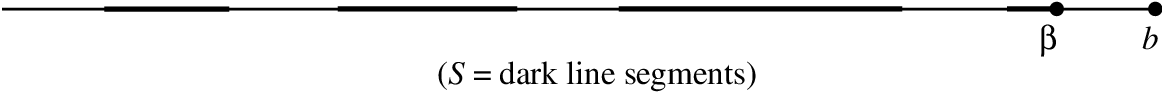
\includegraphics[width=4in,height=.3in]{png/fig010101.png}
\end{center}
\vskip6pt
\refstepcounter{figure}
\centerline{\bf Figure \thefigure} \label{figure:1.1.1}
\vskip12pt

\begin{example}\label{example:1.1.1}\rm
If $S$ is the set of negative numbers, then any nonnegative number is
an upper bound of $S$, and
$\sup S=0$.
If $S_1$ is the set of negative integers, then any number $a$ such that $a
\ge-1$ is an upper bound of $S_1$, and
$\sup S_1=-1$.
\bbox\end{example}

This example shows that a supremum of a set may or may not be
in the set, since $S_1$ contains its supremum, but $S$ does
not.

A {\it nonempty\/} set is a
set that has at least one member.
The {\it empty set},
 denoted by $\emptyset$, is the set that has
no members. Although it may seem foolish to speak of such a set, we
will see that it is a useful idea.

\boxit{The Completeness Axiom}
It is one thing to define an object and another to show that there
really is
an object that satisfies the definition. (For example, does it make
sense to define the smallest positive real number?) This observation
is particularly appropriate in connection with the definition of the
supremum of a set. For example, the empty set is bounded
above by every real number, so it has no supremum.
(Think about this.) More importantly, we will see in
Example~\ref{example:1.1.2} that
properties \part{A}--\part{H} do not guarantee that every nonempty set
that is bounded above has a supremum. Since this property is
indispensable to the rigorous development of calculus,  we
 take it as an axiom for the real numbers.

\begin{Alist}
\setcounter{lcal}{8}
\item % (I)
 If a nonempty set of real numbers  is bounded
above, then it has a supremum.
\end{Alist}

\samepage{Property \part{I} is called {\it
completeness\/},
 and we say that
the real number system is a {\it complete ordered
field.\/}
It can
be shown that the real number system is essentially the only complete
ordered field; that is, if an alien from another planet were to
construct a mathematical system with properties \part{A}--\part{I},
the alien's system would differ from the real number system only in
that the alien might use different symbols for the real numbers and
$+$, $\cdot$, and~$<$.

\begin{theorem}\label{thmtype:1.1.3}
If a nonempty set $S$ of real numbers  is bounded above$,$ then
$\sup S$ is the unique real number $\beta$ such that
\begin{alist}
\item % (a)
 $x\le\beta$ for all $x$ in $S;$
\item % (b)
 if $\epsilon>0$ $($no matter how small$)$$,$ there is an $x_0$ in
$S$ such that
$x_0>
\beta-\epsilon.$
\end{alist}
\end{theorem}}

\newpage

\proof
We first show that $\beta=\sup S$ has properties \part{a} and
\part{b}. Since $\beta$ is an upper bound of $S$, it must satisfy
\part{a}. Since any real number $a$ less than $\beta$ can be written
as $\beta-\epsilon$ with $\epsilon=\beta-a>0$, \part{b} is just
another way of saying that no number less than $\beta$ is an upper
bound of $S$. Hence, $\beta=\sup S$ satisfies \part{a} and \part{b}.

Now we show that there cannot be more than one real number with
properties \part{a} and \part{b}. Suppose that $\beta_1<\beta_2$ and
$\beta_2$ has property \part{b}; thus, if $\epsilon>0$, there is an
$x_0$ in $S$ such that $x_0>\beta_2-\epsilon$. Then, by taking
$\epsilon=\beta_2-\beta_1$, we see that there is an $x_0$ in $S$ such
that
$$
x_0>\beta_2-(\beta_2-\beta_1)=\beta_1,
$$
so  $\beta_1$ cannot have property \part{a}. Therefore, there cannot
be more than one real number that satisfies both \part{a} and
\part{b}.
\bbox

\boxit{Some Notation}
 We will often define
a set $S$ by writing
$S=\set{x}{\cdots}$,
which means that $S$ consists of all $x$ that satisfy the conditions
to the right of the vertical bar; thus, in Example~\ref{example:1.1.1},
\begin{equation}\label{eq:1.1.8}
S=\set{x}{x<0}
\end{equation}
and
$$
S_1=\set{x}{x\mbox{ is a negative integer}}.
$$
We will sometimes abbreviate ``$x$ is a member  of $S$'' by
$x\in S$,
and ``$x$ is not a member of $S$'' by
$x\notin S$.
For example, if $S$ is defined by \eqref{eq:1.1.8}, then
$$
-1\in S\mbox{\quad but \quad} 0\notin S.
$$

\samepage{
\boxit{The Archimedean Property}
The property of the real numbers described in the next theorem is
called the
{\it Archimedean property\/}.
 Intuitively, it states
that it is possible to exceed any positive number, no matter how
large, by adding an arbitrary positive number, no matter how
small, to itself sufficiently many times.

%###
\begin{theorem}
[\href{http://www-history.mcs.st-and.ac.uk/Mathematicians/Archimedes.html}
{Archimedean} Property]
\label{thmtype:1.1.4}
If $\rho$ and $\epsilon$ are positive$,$ then $n\epsilon>\rho$ for
some integer $n.$ \end{theorem}

\proof
The proof is by contradiction.
If the statement is false, $\rho$ is an upper bound of
the set
$$
S=\set{x}{x=n\epsilon,\mbox{$n$ is an integer}}.
$$
Therefore, $S$  has a supremum $\beta$, by property \part{I}.
Therefore,
\begin{equation}\label{eq:1.1.9}
n\epsilon\le\beta \mbox{\quad for all integers $n$}.
\end{equation}}

\newpage\noindent
Since $n+1$ is an integer whenever $n$ is, \eqref{eq:1.1.9} implies that
$$
(n+1)\epsilon\le\beta
$$
 and therefore
$$
n\epsilon\le\beta-\epsilon
$$
  for all integers $n$. Hence,
 $\beta-\epsilon$ is an upper bound of $S$.  Since $\beta-\epsilon
<\beta$, this contradicts the definition of~$\beta$.
\bbox

\boxit{Density of the Rationals and Irrationals}
\helpbox
\begin{definition} \label{thmtype:1.1.5}
A set $D$  is  {\it dense in the reals\/}
if every open interval $(a,b)$  contains a member of $D$.
\end{definition}

\begin{theorem}\label{thmtype:1.1.6}
The rational numbers are dense in the reals$\,;$ that is, if $a$
and
$b$ are real numbers with $a<b,$ there is a rational number $p/q$
such that $a<p/q<b$.
\end{theorem}

\proof
From Theorem~\ref{thmtype:1.1.4} with $\rho=1$ and $\epsilon=b-a$, there
is
a positive integer $q$ such that $q(b-a)>1$. There is also an integer
$j$ such that $j>qa$. This is obvious if $a\le0$, and it follows from
Theorem~\ref{thmtype:1.1.4} with $\epsilon=1$ and $\rho=qa$ if $a>0$. Let
$p$ be the smallest integer such that $p>qa$. Then $p-1\le qa$, so
$$
qa<p\le qa+1.
$$
Since $1<q(b-a)$, this implies that
$$
qa<p<qa+q(b-a)=qb,
$$
so $qa<p<qb$. Therefore, $a<p/q<b$.
\bbox

\begin{example} \label{example:1.1.2}\rm
The rational
number system is not
complete; that is, a set of rational numbers may be bounded above (by
rationals), but not have a rational upper bound  less than any
other rational upper bound. To see this, let
$$
S=\set{r}{r\mbox{ is rational and }r^2<2}.
$$

If $r\in S$, then $r<\sqrt2$. Theorem~\ref{thmtype:1.1.6} implies that if
$\epsilon>0$ there is a rational number $r_0$ such that
$\sqrt2-\epsilon<r_0<\sqrt2$, so Theorem~\ref{thmtype:1.1.3} implies that
$\sqrt{2}=\sup S$. However, $\sqrt{2}$ is {\it
irrational\/};
that is, it cannot be written as the ratio of integers
(Exercise \ref{exer:1.1.3}). Therefore, if $r_1$ is any rational upper
bound of $S$, then $\sqrt{2}<r_1$. By Theorem~\ref{thmtype:1.1.6}, there
is
a rational number $r_2$ such that $\sqrt{2}<r_2<r_1$. Since $r_2$ is
also a rational upper bound of $S$, this shows that $S$ has no
rational supremum.
\bbox\end{example}
\samepage{
Since the rational numbers have properties \part{A}--\part{H}, but not
\part{I}, this example shows that \part{I} does not follow from
\part{A}--\part{H}.

\begin{theorem}\label{thmtype:1.1.7}
The set of irrational numbers is dense in the reals$\,;$ that is, if
$a$ and $b$ are real numbers with $a<b,$  there is an irrational
number
$t$ such that $a<t<b.$
\end{theorem}}

\newpage

\proof
From Theorem~\ref{thmtype:1.1.6}, there are rational numbers $r_1$ and
$r_2$ such that
\begin{equation} \label{eq:1.1.10}
a<r_1<r_2<b.
\end{equation}
Let
$$
t=r_1+\frac{1}{\sqrt2}(r_2-r_1).
$$
Then $t$ is irrational (why?) and $r_1<t<r_2$, so $a<t<b$, from
\eqref{eq:1.1.10}.
\bbox

\boxit{Infimum of a Set}
A set $S$ of real numbers is {\it bounded below\/}  if there is a real
number $a$ such that $x\ge a$ whenever $x\in S$. In this case, $a$ is
a
{\it
lower bound\/} of $S$. If $a$
is a lower bound of
$S$, so is any
smaller number, because of property \part{G}. If $\alpha$ is a lower
bound of $S$, but no number greater than $\alpha$ is, then $\alpha$ is
an {\it infimum\/} of $S$, and we write
$$
\alpha=\inf S.
$$
Geometrically, this means that
there are no points of $S$ to the left of $\alpha$, but there is at
least one point of $S$ to the left of any number greater than
$\alpha$.

\begin{theorem}\label{thmtype:1.1.8}
If a nonempty set $S$ of real numbers  is bounded below$,$ then
$\inf S$ is the unique real number $\alpha$ such that
\begin{alist}
\item % \part{a}
 $x\ge\alpha$ for all $x$ in $S;$
\item % (b)
 if $\epsilon>0$ $($no matter how small$\,)$, there is an $x_0$ in $S$
such that
$x_0<
\alpha+\epsilon.$
\end{alist}
\end{theorem}

\proof (Exercise~\ref{exer:1.1.6})

A set $S$ is {\it bounded\/} if
there are numbers
$a$ and
$b$ such
that $a\le x\le b$ for all $x$ in $S$. A bounded nonempty set has a
unique supremum and a unique infimum, and
\begin{equation}\label{eq:1.1.11}
\inf S\le\sup S
\end{equation}
(Exercise~\ref{exer:1.1.7}).
\bbox

\boxit{The Extended Real Number System}
\hspace*{-.4em}A nonempty set $S$ of real numbers is {\it unbounded
above\/}
if it has no upper bound,  or {\it unbounded below\/}  if it
has no lower bound.
It is convenient to adjoin to the real number system two fictitious
points, $+\infty$ (which we usually write more simply as $\infty$) and
$-\infty$, and to define the order relationships between them and any
real number $x$ by
\begin{equation}\label{eq:1.1.12}
-\infty<x<\infty.
\end{equation}
We call $\infty$  and $-\infty$ {\it points at
infinity\/}. If $S$ is a nonempty set of
reals, we write
\begin{equation}\label{eq:1.1.13}
\sup S=\infty
\end{equation}
to indicate that $S$ is unbounded above,
and
\begin{equation}\label{eq:1.1.14}
\inf S=-\infty
\end{equation}
to indicate that $S$ is  unbounded below.

\begin{example}\label{example:1.1.3}\rm If
$$
S=\set{x}{x<2},
$$
then $\sup S=2$ and $\inf S=-\infty$. If
$$
S=\set{x}{x\ge-2},
$$
then
$\sup
S=\infty$ and $\inf S=-2$. If $S$ is the set of all integers, then
$\sup S=\infty$ and $\inf S=-\infty$.
\bbox\end{example}

The real number system with $\infty$ and $-\infty$ adjoined is called
the {\it extended real number system\/}, or simply the {\it extended
reals}. A member of the
extended reals differing from
$-\infty$ and
$\infty$ is {\it finite\/};
that is, an ordinary real number
is finite. However, the word ``finite'' in ``finite real number'' is
redundant and used only for emphasis, since we would never refer to
$\infty$ or $-\infty$ as real numbers.

The arithmetic relationships among $\infty$, $-\infty$, and the real
numbers are defined as follows.
\begin{alist}
\item % ()
 If $a$ is any real number, then
\begin{eqnarray*}
a+\infty\ar=\phantom{-}\infty+a=\phantom{-}\infty,\\
a-\infty\ar=-\infty+a=-\infty,\\
\dst\frac{a}{\infty}\ar=\dst\frac{a}{-\infty}=0.
\end{eqnarray*}
\item % (b)
  If $a>0$, then
$$
\begin{array}{ccccr}
a\,\infty\ar=\infty\,a\ar=\infty,\\
a\,(-\infty)\ar=(-\infty)\,a\ar=-\infty.
\end{array}
$$
\item % (c)
 If $a<0$, then
$$
\begin{array}{ccccr}
a\,\infty\ar=\infty\,a\ar=-\infty,\\
a\,(-\infty)\ar=(-\infty)\,a\ar=\infty.
\end{array}
$$
\end{alist}

We also define
$$
\infty+\infty=\infty\infty=(-\infty)(-\infty)=\infty
$$
and
$$
-\infty-\infty=\infty(-\infty)=(-\infty)\infty=-\infty.
$$
Finally, we define
$$
|\infty|=|-\infty|=\infty.
$$

The introduction of $\infty$ and $-\infty$, along with the arithmetic
and order relationships defined above, leads to simplifications in the
statements of theorems. For example, the inequality \eqref{eq:1.1.11},
first stated only for bounded sets, holds for any nonempty set $S$ if
it is interpreted properly in accordance with \eqref{eq:1.1.12} and the
definitions of \eqref{eq:1.1.13} and \eqref{eq:1.1.14}.
Exercises~\ref{exer:1.1.10}\part{b} and \ref{exer:1.1.11}\part{b} illustrate
the convenience afforded by some of the arithmetic relationships with
extended reals, and other examples will illustrate this further in
subsequent  sections.

It is not useful to define $\infty-\infty$, $0\cdot\infty$,
$\infty/\infty$, and $0/0$. They are called {\it indeterminate
forms\/}, and left undefined. You probably
studied indeterminate forms
in calculus; we will look at them more carefully in Section~2.4.

\exercises


\begin{exerciselist}
\item\label{exer:1.1.1}
Write the following expressions in equivalent forms not involving
absolute values.

\hspace*{-1em}
\begin{tabular}{l}
\part{a} $a+b+|a-b|$\hspace*{4em}\part{b} $a+b-|a-b|$\\[2\jot]
\part{c} $a+b+2c+|a-b|+\big|a+b-2c+|a-b|\big|$\\[2\jot]
\part{d} $a+b+2c-|a-b|-\big|a+b-2c-|a-b|\big|$\\[2\jot]
\end{tabular}


\item\label{exer:1.1.2}
Verify that the set consisting of two members, $0$ and $1$, with
operations defined by Eqns.~\eqref{eq:1.1.1} and \eqref{eq:1.1.2}, is a
field.
Then show that it is impossible to define an order $<$ on this field
that has properties \part{F}, \part{G}, and \part{H}.

\item\label{exer:1.1.3}
Show that $\sqrt{2}$ is irrational. \hint{Show that if
$\sqrt{2}=m/n,$ where $m$ and $n$ are integers$,$ then both $m$ and
$n$ must be even$.$  Obtain a contradiction from this$.$}

\item\label{exer:1.1.4}
Show that $\sqrt{p}$ is irrational if $p$ is prime.

\item\label{exer:1.1.5}
Find the supremum and infimum of each   $S$.
 State whether they are in $S$.
\begin{alist}
\item % (a)
 $S=\set{x}{x=-(1/n)+\left[1+(-1)^n\right]n^2,
n\ge1}$
\item % (b)
 $S=\set{x}{x^2<9}$
\item % (c)
 $S=\set{x}{x^2\le7}$
\item % (d)
 $S=\set{x}{|2x+1|<5}$
\item % (e)
 $S=\set{x}{(x^2+1)^{-1}>\frac{1}{2}}$
\item % (f)
 $S=\set{x}{x=\mbox{rational and } x^2\le  7}$
\end{alist}

\item\label{exer:1.1.6}
Prove Theorem~\ref{thmtype:1.1.8}. \hint{The set $T=\set{x}{-x\in
S}$ is bounded above if $S$ is bounded below$.$  Apply property {\bf
(I)} and Theorem~$\ref{thmtype:1.1.3}$ to $T.$}

\item\label{exer:1.1.7}
\begin{alist}
\item % (a)
 Show that
$$
\inf\,S\le\sup\,S
\eqno{\rm(A)}
$$
for any nonempty set $S$ of real numbers, and give necessary and
sufficient conditions for equality.
\item % (b)
Show that if $S$ is unbounded then (A) holds if it is interpreted
according to Eqn.~\eqref{eq:1.1.12} and  the definitions of
Eqns.~\eqref{eq:1.1.13} and \eqref{eq:1.1.14}.
\end{alist}

\item\label{exer:1.1.8} Let $S$ and $T$ be nonempty sets of real numbers
such that every real number is in $S$ or $T$ and if $s\in S$ and $t\in
T$, then $s<t$. Prove that there is a unique real number $\beta$ such
that every real number less than $\beta$ is in $S$ and every real
number greater than $\beta$ is in $T$. (A decomposition of the reals
into two sets with these properties is a
\href{http://www-history.mcs.st-and.ac.uk/Mathematicians/Dedekind.html}
{\it Dedekind\/}
{\it cut\/}. This is known as {\it
Dedekind's theorem\/}.)


\item\label{exer:1.1.9} Using properties \part{A}--\part{H} of
the real
numbers and taking Dedekind's theorem (Exercise~\ref{exer:1.1.8})\ as
given, show that every nonempty set $U$ of real numbers that is
bounded above has a supremum. \hint{\/ Let $T$ be the set of
upper bounds of $U$ and $S$ be the set of real numbers that are not
upper bounds of $U.$}

\item\label{exer:1.1.10}  Let $S$ and $T$ be nonempty sets of real numbers
and define
$$
S+T=\set{s+t}{\,s\in S, t\in T}.
$$
\begin{alist}
\item % (a)
Show that
$$
\sup  (S+T)=\sup S+\sup T
\eqno{\rm(A)}
$$
if $S$ and $T$ are bounded above and
$$
\inf  (S+T)=\inf S+\inf T
\eqno{\rm(B)}
$$
if $S$ and $T$ are bounded below.
\item % (b)
Show that if they are properly interpreted in the extended reals, then
(A) and (B) hold if $S$ and $T$ are arbitrary nonempty sets of real
numbers.
\end{alist}

\item\label{exer:1.1.11} Let $S$ and $T$ be nonempty sets of real numbers
and define
$$
S-T=\set{s-t}{s\in S, t\in T}.
$$
\begin{alist}
\item % (a)
Show that if $S$ and $T$ are bounded, then
$$
\sup (S-T)=\sup S-\inf T
\eqno{\rm(A)}
$$
and
$$
\inf (S-T)=\inf S-\sup T.
\eqno{\rm(B)}
$$
\item % (b)
Show that if they are properly interpreted in the extended reals, then
(A) and (B) hold if $S$ and $T$ are arbitrary nonempty sets of real
numbers.

\end{alist}

\item\label{exer:1.1.12}
Let $S$ be a bounded nonempty set of real numbers, and let $a$ and $b$
be fixed real numbers. Define $T=\set{as+b}{s\in S}$. Find formulas
for
$\sup T$ and $\inf T$ in terms of $\sup S$ and $\inf S$. Prove your
formulas.
\label{sectionend:\thesection}
\end{exerciselist}


\currentpdfbookmark{Section 1.2 Mathematical Induction}{section:1.2}
\newsection{2}{The Real Numbers}{Mathematical Induction}



\renewcommand{\thissection}{\sectiontitle{MATHEMATICAL INDUCTION}}
\thissection
\samepage{
\noindent
If a flight of stairs is designed so that falling off any step
inevitably leads to falling off the next, then falling off the first
step is a sure way to end up at the bottom. Crudely expressed, this is
the essence of the {\it principle of mathematical
induction\/}: If
the truth of a statement depending on a given integer $n$ implies the
truth of the corresponding statement with $n$ replaced by $n+1$, then
the statement is true for all positive integers $n$ if it is true for
$n=1$. Although you have probably studied this principle before,
it is so important that it merits careful review here.

\boxit{Peano's Postulates and Induction}
The rigorous construction of the real number system starts with a set
$\mathbb N$ of undefined elements called {\it natural
numbers\/}, with the
following properties.}

\newpage

\begin{Alist}
\item  %(A)
 $\mathbb N$ is nonempty.
\item  %(B)
 Associated with each natural number $n$ there is a unique
natural number $n'$ \phantom{c}called the {\it successor
of\/}
$n$.
\item % (C)
  There is a natural number $\overline{n}$ that is not the
successor of any natural number.
\item % (D)
 Distinct natural numbers have distinct successors; that is,
if $n\ne m$, then \phantom{n}$n'\ne m'$.
\item % (E)
 The only subset of $\mathbb N$ that contains
$\overline{n}$
and the successors of all its elements is \phantom{n}$\mathbb N$
itself.
\end{Alist}

These axioms are known as
\href{http://www-history.mcs.st-and.ac.uk/Mathematicians/Peano.html}
{\it Peano}{\it's postulates\/}.
The real
numbers can be constructed from the natural numbers by definitions and
arguments based on them. This is a formidable task that we will not
undertake. We mention it to show how little you need to start with to
construct the reals and, more important, to draw attention to
postulate \part{E}, which is the basis for the principle of
mathematical induction.

It can be shown that the positive integers form a subset of the reals
that satisfies Peano's postulates (with $\overline{n}=1$ and
$n'=n+1$), and it is customary to regard the positive integers and the
natural numbers as identical. From this point of view, the principle
of mathematical induction is basically a restatement of postulate
\part{E}.

\begin{theorem} [Principle of Mathematical
Induction] \label{thmtype:1.2.1}
 Let $P_1,$ $P_2, $\dots$,$ $P_n,$ \dots\ be
propositions$,$ one
for each positive integer$,$ such that
\begin{alist}
\item % (a)
 $P_1$ is true$;$
\item % (b)
 for each positive integer $n,$  $P_n$  implies $P_{n+1}.$
\end{alist}
Then $P_n$ is true for each positive integer $n.$
\end{theorem}

\proof
  Let
$$
\mathbb M=\set{n}{n\in \mathbb N\mbox{ and } P_n\mbox{ is
true}}.
$$
From \part{a}, $1\in \mathbb M$, and from \part{b}, $n+1\in \mathbb M$ whenever
$n\in \mathbb M$. Therefore, $\mathbb M=\mathbb N$, by postulate
\part{E}.
\bbox

\enlargethispage{\baselineskip}
\begin{example}\label{example:1.2.1}\rm   Let $P_n$ be the
proposition that
\begin{equation}\label{eq:1.2.1}
1+2+\cdots+n=\frac{n(n+1)}{2}.
\end{equation}
Then $P_1$ is the proposition that $1=1$, which is certainly true.  If
$P_n$ is true, then adding $n+1$ to both sides of \eqref{eq:1.2.1} yields
\begin{eqnarray*}
(1+2+\cdots+n)+(n+1)\ar=\frac{n(n+1)}{2}+(n+1)\\
\ar=(n+1)\left(\frac{n}{2}+1\right)\\
\ar=\frac{(n+1)(n+2)}{2},\\
\arraytext{or}\\
1+2+\cdots+(n+1)\ar=\frac{(n+1)(n+2)}{2},
\end{eqnarray*}

\newpage
\noindent
which is $P_{n+1}$, since it has the form of \eqref{eq:1.2.1}, with $n$
replaced by $n+1$. Hence, $P_n$ implies $P_{n+1}$, so
\eqref{eq:1.2.1} is true for all $n$, by Theorem~\ref{thmtype:1.2.1}.
\bbox\end{example}

A proof based on Theorem~\ref{thmtype:1.2.1} is an {\it induction
proof\/},
or {\it proof by induction\/}. The assumption that $P_n$ is true is the
{\it induction assumption\/}.
(Theorem~\ref{thmtype:1.2.3} permits a
kind of induction proof in which the induction assumption takes a
different form.)

Induction, by definition, can be used only to verify results
conjectured by other means. Thus, in Example~\ref{example:1.2.1} we did
not use induction to {\it find\/} the sum
\begin{equation}\label{eq:1.2.2}
s_n=1+2+\cdots+n;
\end{equation}
rather, we {\it verified\/} that
\begin{equation}\label{eq:1.2.3}
s_n=\frac{n(n+1)}{2}.
\end{equation}
How you guess what to prove by induction depends on the problem and
your approach to it. For example, \eqref{eq:1.2.3} might be conjectured
after observing that
$$
s_1=1=\frac{1\cdot2}{2},\quad s_2=3=\frac{2\cdot3}{2},\quad
s_3=6=\frac{4\cdot3}{2}.
$$
However, this requires sufficient insight to recognize that these
results are of the form \eqref{eq:1.2.3} for $n=1$, $2$, and $3$.
Although it is easy to prove \eqref{eq:1.2.3} by induction once it has
been conjectured, induction is not the most efficient way to find
$s_n$, which can be obtained quickly by rewriting \eqref{eq:1.2.2} as
$$
s_n=n+(n-1)+\cdots+1
$$
and adding this to \eqref{eq:1.2.2} to obtain
$$
2s_n=[n+1]+\left[(n-1)+2\right]+\cdots+[1+n].
$$
There are $n$ bracketed expressions on the right, and the terms in
each add up to $n+1$; hence,
$$
2s_n=n(n+1),
$$
which yields \eqref{eq:1.2.3}.

The next two examples deal with problems for which induction is a
natural and efficient method of solution.

\enlargethispage{\baselineskip}
\begin{example}\label{example:1.2.2}\rm   Let $a_1=1$ and
\begin{equation}\label{eq:1.2.4}
a_{n+1}=\frac{1}{n+1}a_n,\quad n\ge1
\end{equation}
(we say that $a_n$ is defined {\it inductively\/}),
 and suppose that we wish to
find an explicit formula for $a_n$.  By considering $n=1$, $2$, and
$3$, we
find that
$$
a_1=\frac{1}{1},\quad a_2=\frac{1}{1\cdot2},\mbox{\quad and\quad}
a_3=\frac{1}{1\cdot2\cdot3},
$$
\newpage
\noindent
and therefore we conjecture that
\begin{equation}\label{eq:1.2.5}
a_n=\frac{1}{n!}.
\end{equation}
This is given for $n=1$.  If we assume it is true for some $n$,
substituting it into \eqref{eq:1.2.4} yields
$$
a_{n+1}=\frac{1}{ n+1} \frac{1}{ n!}=\frac{1}{(n+1)!},
$$
which is  \eqref{eq:1.2.5} with $n$ replaced by $n+1$.
Therefore, \eqref{eq:1.2.5} is true for every positive integer $n$, by
Theorem~\ref{thmtype:1.2.1}.
\end{example}

\begin{example}\label{example:1.2.3}\rm For each nonnegative
integer $n$, let
$x_n$ be a real number and suppose that
\begin{equation}\label{eq:1.2.6}
|x_{n+1}-x_n|\le r |x_n-x_{n-1}|,\quad n\ge1,
\end{equation}
where $r$ is a fixed positive number. By considering \eqref{eq:1.2.6} for
$n=1$, $2$, and $3$, we find that
$$
\begin{array}{lllll}
|x_2-x_1|\ar\le r|x_1-x_0|,\\
|x_3-x_2|\ar\le r|x_2-x_1|\le r^2|x_1-x_0|,\\
|x_4-x_3|\ar\le r|x_3-x_2|\le r^3|x_1-x_0|.
\end{array}
$$
Therefore, we conjecture that
\begin{equation}\label{eq:1.2.7}
|x_n-x_{n-1}|\le r^{n-1}|x_1-x_0|
\mbox{\quad if\quad}n\ge1.
\end{equation}
 This is trivial for $n=1$.  If it is
true for some $n$, then \eqref{eq:1.2.6} and \eqref{eq:1.2.7} imply that
$$
|x_{n+1}-x_n|\le r(r^{n-1}|x_1-x_0|),\mbox{\quad so\quad}
|x_{n+1}-x_n|\le r^n|x_1-x_0|,
$$
which is proposition \eqref{eq:1.2.7} with $n$ replaced by $n+1$. Hence,
\eqref{eq:1.2.7} is true for every positive integer $n$, by
Theorem~\ref{thmtype:1.2.1}.
\bbox\end{example}

The major effort in an induction proof (after
$P_1$, $P_2$, \dots, $P_n$, \dots\
have been formulated) is usually directed toward showing that $P_n$ implies
$P_{n+1}$.  However, it is  important to verify $P_1$, since $P_n$
may imply $P_{n+1}$ even if some or all of the propositions
$P_1$, $P_2$, \dots, $P_n$, \dots\ are false.

\begin{example}\label{example:1.2.4}\rm  Let $P_n$ be the
proposition that
$2n-1$ is divisible by $2$. If $P_n$ is true then $P_{n+1}$ is also,
since
$$
2n+1=(2n-1)+2.
$$
However, we cannot conclude that $P_n$ is true for $n\ge1$. In fact,
$P_n$ is false for every~$n$.
\bbox\end{example}

The following formulation of the  principle of mathematical
induction permits us to start
induction proofs with an arbitrary integer, rather than 1, as required in
Theorem~\ref{thmtype:1.2.1}.

\begin{theorem}\label{thmtype:1.2.2}
 Let $n_0$ be any integer $($positive$,$
 negative$,$ or zero$)$$.$ Let
$P_{n_0},$ $P_{n_0+1},$ \dots$,$ $P_n,$ \dots\ be propositions$,$
 one for each integer $n\ge n_0,$ such that
\begin{alist}
\item % (a)
 $P_{n_0}$ is true$\,;$
\item % (b)
 for each integer $n\ge n_0,$ $P_n$  implies $P_{n+1}.$
\end{alist}
Then $P_n$ is true for every integer  $n\ge n_0.$
\end{theorem}

\proof
For $m\ge1$, let  $Q_m$ be the proposition defined by
$Q_m=P_{m+n_0-1}$. Then $Q_1=P_{n_0}$ is true by \part{a}.
If $m\ge1$ and $Q_m=P_{m+n_0-1}$ is true, then $Q_{m+1}=P_{m+n_0}$
is true by \part{b} with $n$ replaced by $m+n_0-1$. Therefore,
$Q_m$ is true for all $m\ge1$ by Theorem~\ref{thmtype:1.2.1} with $P$
replaced by $Q$ and $n$ replaced by $m$. This is equivalent
to the statement that $P_n$ is true for all $n\ge n_0$.
\bbox

\begin{example}\label{example:1.2.5}\rm  Consider the
proposition $P_n$ that
$$
3n+16>0.
$$
If $P_n$ is true, then so is $P_{n+1}$, since
\begin{eqnarray*}
3(n+1)+16\ar=3n+3+16\\\ar=(3n+16)+3>0+3 \mbox{ (by the induction
assumption)}\\
\ar>0.
\end{eqnarray*}
The smallest $n_0$ for which $P_{n_0}$ is true is $n_0=-5$. Hence,
$P_n$ is true for $n\ge-5$, by Theorem~\ref{thmtype:1.2.2}.
\end{example}

\begin{example}\label{example:1.2.6}\rm   Let $P_n$ be the
proposition that
$$
n!-3^n>0.
$$
If $P_n$ is true, then
\begin{eqnarray*}
(n+1)!-3^{n+1}\ar=n!(n+1)-3^{n+1}\\
\ar>3^n(n+1)-3^{n+1} \mbox{\quad (by the induction assumption)}\\
\ar=3^n(n-2).
\end{eqnarray*}
Therefore, $P_n$ implies $P_{n+1}$ if $n>2$.  By trial and error,
$n_0=
7$ is the smallest integer such that $P_{n_0}$ is true; hence, $P_n$
is true for $n\ge7$, by Theorem~\ref{thmtype:1.2.2}.
\bbox\end{example}

\samepage{The next theorem is a useful consequence of the principle
of mathematical induction.

\begin{theorem}\label{thmtype:1.2.3}
 Let $n_0$ be any integer $($positive$,$
 negative$,$ or zero$)$$.$ Let
$P_{n_0},$ $P_{n_0+1}, $\dots$,$ $P_n,$ \dots\ be propositions$,$
 one for each integer $n\ge n_0,$ such that
\begin{alist}
\item % (a)
 $P_{n_0}$ is true$\,;$
\item % (b)
for $n\ge n_0,$ $P_{n+1}$ is true if $P_{n_0},$ $P_{n_0+1}, $\dots$,$
$P_n$ are all true.
\end{alist}
Then $P_n$ is true for $n\ge n_0.$
\end{theorem}}

\newpage
\proof
For $n\ge n_0$,  let $Q_n$ be the proposition that
 $P_{n_0}$, $P_{n_0+1}$, \dots, $P_n$ are all true.
Then $Q_{n_0}$ is true by \part{a}. Since $Q_n$ implies $P_{n+1}$
by \part{b}, and $Q_{n+1}$ is true if $Q_n$ and $P_{n+1}$ are both true,
Theorem~\ref{thmtype:1.2.2} implies that $Q_n$ is true for all $n\ge
n_0$. Therefore, $P_n$ is true for all $n\ge  n_0$.
\bbox

\begin{example}\label{example:1.2.7}\rm   \rm
An integer $p>1$ is a {\it prime\/}
if it cannot be factored as
$p=rs$
where $r$ and $s$ are integers and $1<r$, $s<p$. Thus, 2, 3, 5, 7, and
11 are primes, and, although 4, 6, 8, 9, and 10 are not, they are
products of primes:
$$
4=2\cdot2,\quad 6=2\cdot3,\quad 8=2\cdot2\cdot2,\quad 9=
3\cdot3,\quad 10=2\cdot5.
$$
These observations suggest that each integer $n\ge2$
 is a prime or a product of primes. Let this proposition be $P_n$.
Then
$P_2$ is true, but
neither Theorem~\ref{thmtype:1.2.1} nor Theorem~\ref{thmtype:1.2.2} apply,
since $P_n$ does not imply $P_{n+1}$ in any obvious way. (For example,
it is not evident from $24=2\,\cdot2\,\cdot2\,\cdot3$ that 25 is a
product of primes.) However, Theorem~\ref{thmtype:1.2.3} yields the stated
result, as follows. Suppose that $n\ge2$ and $P_2$, \dots, $P_n$ are true.
Either $n+1$ is a prime or
\begin{equation}\label{eq:1.2.8}
n+1=rs,
\end{equation}
where $r$ and $s$ are integers and $1<r$, $s<n$, so  $P_r$ and
$P_s$ are true by assumption. Hence, $r$ and $s$ are primes or
products of primes and \eqref{eq:1.2.8} implies that $n+1$ is a product
of primes. We have now proved $P_{n+1}$ (that $n+1$ is a prime or a
product of primes).  Therefore, $P_n$ is true for all $n\ge2$, by
Theorem~\ref{thmtype:1.2.3}.
\end{example}

\exercises
{\it Prove  the assertions in
Exercises~$\ref{exer:1.2.1}$--$\ref{exer:1.2.6}$ by
induction.\/}

\begin{exerciselist}
\item\label{exer:1.2.1}
  The sum of the first $n$ odd integers is $n^2$.

\item\label{exer:1.2.2}
$\dst 1^2+2^2+\cdots+n^2=\frac{n(n+1)(2n+1)}{6}.$

\item\label{exer:1.2.3}
$\dst 1^2+3^2 + \cdots + (2n-1)^2 = \frac{n(4n^2-1)}{ 3}.$

\item\label{exer:1.2.4}
 If $a_1$, $a_2$, \dots, $a_n$ are arbitrary real numbers,
then
$$
|a_1+a_2+\cdots+a_n|\le|a_1|+|a_2|+\cdots+|a_n|.
$$

\item\label{exer:1.2.5}
If $a_i\ge0$, $i\ge1$, then
$$
(1+a_1)(1+a_2)\cdots (1+a_n)\ge1+a_1+a_2+\cdots+a_n.
$$

\item\label{exer:1.2.6}
  If $0\le a_i\le1$, $i\ge1$, then
$$
(1-a_1)(1-a_2)\cdots (1-a_n)\ge1-a_1-a_2\cdots-a_n.
$$

\item\label{exer:1.2.7}
Suppose that $s_0>0$ and $s_n=1-e^{-s_{n-1}}$, $n\ge1$.  Show that
$0<s_n<1$, $n\ge 1$.

\item\label{exer:1.2.8} Suppose that $R>0$, $x_0>0$, and
$$
x_{n+1}=\frac{1}{2}\left(\frac{R}{x_n}+x_n\right),\quad n\ge0.
$$
Prove:  For $n\ge1$, $x_n>x_{n+1}>\sqrt{R}$ and
$$
x_n-\sqrt{R}\le \frac{1}{2^n}\frac{(x_0-\sqrt{R})^2}{ x_0}.
$$

\item\label{exer:1.2.9}
Find and prove by induction an explicit formula for $a_n$ if
$a_1=1$ and, for $n\ge~1$,

\begin{tabular}[t]{@{}p{168pt}@{}p{168pt}}
\part{a} $\dst{a_{n+1}=\frac{a_n}{(n+1)(2n+1)}}$&\part{b}
$\dst a_{n+1}=\frac{3a_n}{(2n+2)(2n+3)}$\\\\
\part{c} $\dst{a_{n+1}=\frac{2n+1}{ n+1}a_n}$&\part{d}
$\dst{a_{n+1}=\left(1+\frac{1}{n}\right)^n a_n}$
\end{tabular}

\item\label{exer:1.2.10}
Let $a_1=0$ and $a_{n+1}=(n+1)a_n$ for $n\ge1$, and let $P_n$
be the proposition that $a_n=n!$
\begin{alist}
\item % (a)
 Show that $P_n$ implies $P_{n+1}$.
\item % (b)
 Is there an integer $n$ for which $P_n$ is true?
\end{alist}

\item\label{exer:1.2.11}
Let $P_n$ be the proposition that
$$
1+2+\cdots+n=\frac{(n+2)(n-1)}{2}.
\begin{tabular}[t]{@{}p{168pt}@{}p{168pt}}
\end{tabular}
$$
\begin{alist}
\item % (a)
 Show that $P_n$ implies $P_{n+1}$.
\item % (b)
Is there an integer $n$ for which $P_n$ is true?
\end{alist}

\item\label{exer:1.2.12}
For what integers $n$ is
$$
\frac{1}{ n!}>\frac{8^n}{(2n)!}\,?
$$
Prove your answer by induction.

\samepage{
\item\label{exer:1.2.13}
Let $a$ be an integer $\ge2$.
\begin{alist}
\item % (a)
 Show by induction that if $n$ is a
nonnegative integer, then $n=aq+r$, where $q$ (quotient)
and $r$ (remainder) are integers and $0\le r<a$.
\item % (b)
 Show that the result of \part{a} is true if $n$ is an
arbitrary integer (not necessarily nonnegative).
\item % (c)
Show that there is only one way to write a given integer $n$ in the
form $n=aq+r$, where $q$ and $r$ are integers and $0\le r<a$.
\end{alist}

\item\label{exer:1.2.14}
Take the following statement as given: If $p$ is a prime and $a$ and
$b$ are integers such that $p$ divides the product $ab$, then $p$
divides $a$ or $b$.}

\newpage
\begin{alist}
\item % (a)
Prove: If $p$, $p_1$, \dots, $p_k$ are positive primes and $p$ divides
the product $p_1\cdots p_k$, then $p=p_i$ for some $i$ in
$\{1, \dots,k\}$.
\item % (b)
 Let
$n$ be an integer $>1$. Show that the prime factorization of $n$ found
in Example~\ref{example:1.2.7} is unique in the following sense: If
$$
n=p_1\cdots p_r\mbox{\quad and\quad} n=q_1q_2\cdots q_s,
$$
where $p_1$, \dots, $p_r$, $q_1$, \dots, $q_s$ are positive primes,
then
$r=s$ and $\{q_1, \dots,q_r\}$ is a permutation of
$\{p_1,\dots,p_r\}$.
\end{alist}

\item\label{exer:1.2.15}
Let $a_1=a_2=5$ and
$$
a_{n+1}=a_n+6a_{n-1},\quad n\ge2.
$$
Show by induction that $a_n=3^n-(-2)^n$ if $n\ge1$.

\item\label{exer:1.2.16}
Let $a_1=2$, $a_2=0$, $a_3=-14$, and
$$
a_{n+1}=9a_n-23a_{n-1}+15a_{n-2},\quad n\ge3.
$$
Show by induction that $a_n=3^{n-1}-5^{n-1}+2$, $n\ge1$.

\item\label{exer:1.2.17}
The
\href{http://www-history.mcs.st-and.ac.uk/Mathematicians/Fibonacci.html}
{\it Fibonacci\/}
{\it  numbers\/}
$\{F_n\}_{n=1}^\infty$ are defined by $F_1=F_2=1$ and
$$
F_{n+1}=F_n+F_{n-1}, \quad n \ge 2.
$$
Prove by induction that
$$
F_n=\frac{(1+\sqrt5)^n-(1-\sqrt5)^n}{2^n\sqrt5},\quad n\ge1.
$$

\samepage{
\item\label{exer:1.2.18}
Prove by induction that
$$
\int_0^1 y^n(1-y)^r\,dy=\frac{n!}{(r+1)(r+2)\cdots(r+n+1)}
$$
if $n$ is a nonnegative integer and $r>-1$.

\item\label{exer:1.2.19}
Suppose that $m$ and $n$ are integers, with $0\le m\le n$. The {\it
binomial coefficient}
$\dst\binom{n}{ m}$
is the coefficient of $t^m$ in the expansion of $(1+t)^n$; that is,
$$
(1+t)^n=\sum_{m=0}^n\binom{n}{m}t^m.
$$
From this definition it follows immediately that
$$
\binom{n}{ 0}=\binom{n}{ n}=1,\quad n\ge0.
$$
For convenience we define
$$
\binom{n}{-1\phantom{-}}=\binom{n}{ n+1}=0,\quad
n\ge0.
$$}

\newpage
\begin{alist}
\item % (a)
 Show that
$$
\binom{n+1}{ m}=\binom{n}{ m}+\binom{n}{ m-1},\quad 0\le m\le n,
$$
and use this to show by induction on $n$ that
$$
\binom{n}{ m}=\frac{n!}{m!(n-m)!},\quad 0\le m\le n.
$$
\item % (b)
 Show that
 $$
\sum^n_{m=0}(-1)^m\binom{n}{m}=0\mbox{\quad and \quad}
\sum^n_{m=0}\binom{n}{m}=2^n.
$$
\item % (c)
Show that
$$
(x+y)^n=\sum_{m=0}^n\binom{n}{m}x^my^{n-m}.
$$
(This is the {\it  binomial theorem\/}.)
\end{alist}

\item\label{exer:1.2.20}
Use induction to find an $n$th
antiderivative of $\log x$, the natural logarithm of~$x$.

\item\label{exer:1.2.21}
Let $f_1(x_1)=g_1(x_1)=x_1$. For $n\ge2$, let
\begin{eqnarray*}
f_n(x_1,x_2, \dots,x_n)\ar=f_{n-1}(x_1,x_2,
\dots,x_{n-1})+2^{n-2}x_n+\\
&&|f_{n-1}(x_1,x_2, \dots,x_{n-1})-2^{n-2}x_n|
\end{eqnarray*}
and
\begin{eqnarray*}
g_n(x_1,x_2, \dots,x_n)\ar=g_{n-1}(x_1,x_2,
\dots,x_{n-1})+2^{n-2}x_n-\\
&&|g_{n-1}(x_1,x_2, \dots,x_{n-1})-2^{n-2}x_n|.
\end{eqnarray*}
Find explicit formulas for  $f_n(x_1,x_2, \dots,x_n)$
and $g_n(x_1,x_2, \dots,x_n)$.
%\hint{See Exercise~\ref{exer:1.1.1}\part{a} and \part{b}$.$}


\item\label{exer:1.2.22}
Prove by induction that
$$
\sin x+\sin3x+\cdots+\sin(2n-1)x=\frac{1-\cos2nx}{ 2\sin x},\quad
n\ge1.
$$
\hint{You will need  trigonometric identities
that you can derive from the identities
\begin{eqnarray*}
\cos(A-B)\ar=\cos A\cos B+\sin A\sin B,\\
\cos(A+B)\ar=\cos A\cos B-\sin A\sin B.
\end{eqnarray*}
Take these two identities as given$.$}

\item\label{exer:1.2.23}
Suppose that $a_1\le a_2\le\cdots\le a_n$ and $b_1\le b_2\le\cdots\le
b_n$. Let $\{\ell_1,\ell_2, \dots\ell_n\}$ be a permutation of $\{1,2,
\dots,n\}$, and define
$$
Q(\ell_1,\ell_2, \dots,\ell_n)=\sum_{i=1}^n(a_i-b_{\ell_i})^2.
$$
Show that
$$
Q(\ell_1,\ell_2, \dots,\ell_n)\ge Q(1,2, \dots,n).
$$

\label{sectionend:\thesection}
\end{exerciselist}

\currentpdfbookmark{Section 1.3 The Real Line}{section:1.3}
\newsection{3}{The Real Numbers}{The Real Line}
\renewcommand{\thissection}{\sectiontitle{THE REAL LINE}}
\thissection


\noindent
One of our objectives is to develop rigorously
the concepts of limit, continuity,
differentiability,
and integrability, which you have  seen in calculus.
To do this requires a better understanding of the
real numbers than is  provided in calculus. The
purpose of this section is to develop this understanding. Since the
utility of the concepts introduced here will not become apparent until
we are well into the study of limits and continuity, you should
 reserve judgment on their value until they are applied. As this
occurs, you should reread the applicable parts of this
section. This  applies especially to the concept of an open
covering and to the Heine--Borel and
Bolzano--Weierstrass theorems,
which will seem mysterious at first.

We assume that you are familiar with the geometric interpretation of
the real numbers as points on a line. We will not prove that this
interpretation is legitimate, for two reasons: (1) the proof
requires an excursion into the  foundations of Euclidean
geometry, which is not the purpose of this book; (2) although
we will use geometric terminology and intuition in discussing the
reals, we will base all proofs on properties \part{A}--\part{I}
(Section~1.1) and their consequences, not on geometric arguments.

Henceforth, we will use the terms {\it real number
system\/} and
{\it
real line\/} synonymously and denote both by the
symbol
$\R$;
also, we will often refer to a real number as a {\it
point\/}
(on the real line).

\boxit{Some Set Theory}
In this section we are interested  in sets of points on
the real line; however,  we will consider other kinds of sets in
subsequent
sections. The following definition applies to arbitrary sets, with the
understanding that the members of all sets under consideration
in any given context come from
a specific collection of elements, called the {\it universal
set\/}. In
this section the universal set is the real numbers.

\enlargethispage{\baselineskip}
\begin{definition}\label{thmtype:1.3.1}
 Let $S$ and $T$ be sets.
\begin{alist}
\item % (a)
$S$ {\it contains\/} $T$, and we write $S\supset T$ or $T\subset
S$, if every member of $T$ is also in $S$. In this case, $T$ is
a {\it subset\/} of $S$.
\item % (b)
 $S-T$ is the set of elements that are in $S$ but not in $T$.
\item % (c)
$S$ {\it equals\/} $T$, and we write $S=T$,
if
$S$ contains
$T$ and
$T$ contains $S$; thus, $S=T$ if and only if $S$ and $T$ have the same
members.

\newpage
\item % (d)
 $S$ {\it strictly contains\/} $T$
if $S$ contains $T$ but $T$ does not contain $S$; that
is, if every member of  $T$ is also in $S$, but at least one member
of
$S$ is not in $T$ (Figure~\ref{figure:1.3.1}).
\item % (e)
The {\it complement\/}  of $S$, denoted by $S^c$,
is the set of elements in the universal set that are not in $S$.
\item % (f)
 The {\it union\/} of $S$
and
$T$, denoted by
$S\cup T$, is the set of elements in at least one of $S$ and $T$
(Figure~\ref{figure:1.3.1}\part{b}).
\item % (g)
The {\it intersection\/}  of $S$ and $T$, denoted by
$S\,\cap\, T$, is the
set of elements in both $S$ and $T$ (Figure~\ref{figure:1.3.1}\part{c}).
If $S\cap T=\emptyset$ (the empty set), then $S$ and $T$ are
 {\it disjoint sets\/}
(Figure~\ref{figure:1.3.1}\part{d}).
\item % (h)
 A set with only one member $x_0$ is a {\it singleton
set\/},  denoted by
$\{x_0\}$.
\end{alist}
\end{definition}

\vskip-6.1pt
\begin{center}
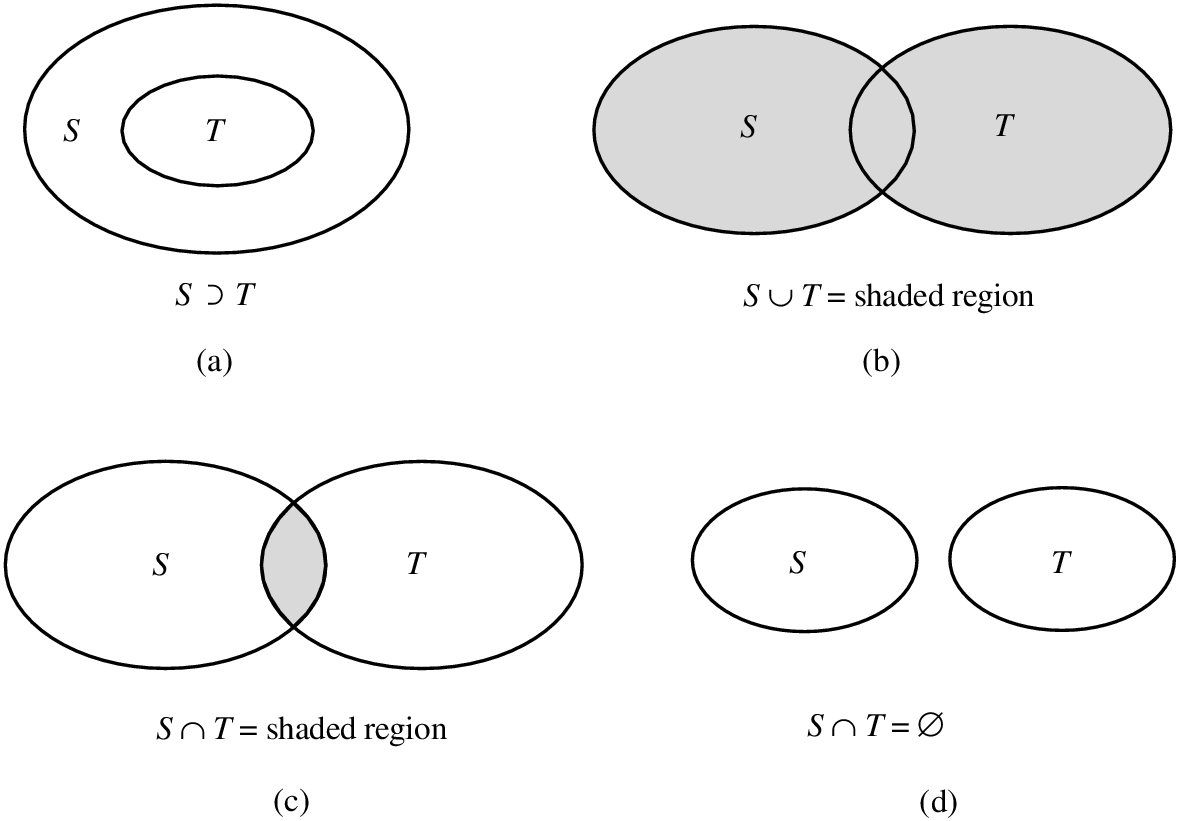
\includegraphics[width=4in,height=2.875in]{png/fig010301.png}
\end{center}
\vskip6pt
\refstepcounter{figure}
\centerline{\bf Figure \thefigure} \label{figure:1.3.1}
\vskip6pt
%\vskip12pt

\enlargethispage{\baselineskip}
\begin{example}\label{example:1.3.1}\rm  Let
$$
S=\set{x}{0<x<1},\quad  T=\set{x}{0<x<1 \mbox{ and $x$ is
rational}},
$$
and
$$
U=\set{x}{0<x<1\mbox{ and $x$ is irrational}}.
$$

Then $S\supset T$ and $S\supset U$, and the inclusion is strict in
both cases.
 The unions of pairs of these sets are
$$
S\cup T=S,\quad S\cup U=S,\mbox{\quad and\quad} T\cup U=S,
$$
and their intersections are
$$
S\cap T=T,\quad S\cap U=U,\mbox{\quad and\quad} T\cap U=
\emptyset.
$$
\newpage
\noindent
Also,
$$
 S-U=T\mbox{\quad and\quad}S-T=U.
\eqno{\bbox}
$$
\end{example}

Every set $S$ contains the empty set $\emptyset$, for to say that
$\emptyset$ is
not contained in $S$ is to say that some member of $\emptyset$ is not
in $S$, which is absurd since $\emptyset$ has no members.
If $S$ is any set, then
$$
(S^c)^c=S\mbox{\quad and\quad} S\cap S^c=\emptyset.
$$
If $S$ is a set of real numbers, then $S\cup S^c=\R$.

The definitions of union and intersection have
generalizations: If ${\mathcal F}$ is an arbitrary collection of sets,
then $\cup\set{S}{S\in {\mathcal F}}$ is the set of all elements that
are members
of at least one of the sets in ${\mathcal F}$, and $\cap\set{S}{S\in {\mathcal
F}}$ is the set of all elements that are members of every set in
${\mathcal
F}$. The union and intersection of finitely many sets $S_1$, \dots,
$S_n$
are also written as $\bigcup^n_{k=1}S_k$ and $\bigcap^n_{k=1}S_k$. The
union and intersection of an infinite sequence $\{S_k\}_{k=1}^\infty$
of sets are written as
$\bigcup^\infty_{k=1}S_k$ and $\bigcap^\infty_{k=1}S_k$.

\vskip1pc
\begin{example}\label{example:1.3.2}\rm
 If ${\mathcal F}$ is the collection of sets
$$
S_\rho=\set{x}{\rho<x\le1+\rho},\quad  0<\rho\le1/2,
$$
then
$$
 \bigcup\set{S_\rho}{S_\rho\in {\mathcal F}}=\set{x}{0<x\le3/2}
\mbox{\ and \ }\bigcap\set{S_\rho}{S_\rho\in {\mathcal F}}=
\set{x}{1/2<x\le1}.
$$
\end{example}

\vskip1pc
\begin{example} \label{example:1.3.3}\rm
If, for each positive integer $k$, the set  $S_k$ is the set of real
numbers that can be written as $x=m/k$ for some integer $m$, then
$\bigcup^\infty_{k=1}S_k$ is the set of rational numbers and
$\bigcap^\infty_{k=1}S_k$ is the set of integers.
\end{example}

\vskip1pc
\boxit{Open and Closed Sets}
If $a$ and $b$ are in the extended reals and $a<b$, then the
{\it open interval\/}
$(a,b)$ is defined by
$$
(a,b)=\set{x}{a<x<b}.
$$
The open intervals $(a,\infty)$ and $(-\infty,b)$ are {\it
semi-infinite} if $a$ and $b$ are
finite, and
$(-\infty,\infty)$ is the entire real line.

\vskip1pc
\begin{definition}\label{thmtype:1.3.2}
If $x_0$ is a real number and $\epsilon>0$, then the open interval
$(x_0-\epsilon, x_0+\epsilon)$ is an {\it $\epsilon$-neighborhood\/}
of
$x_0$.
If a set $S$ contains an $\epsilon$-neighborhood of $x_0$, then $S$ is a
{\it neighborhood\/} of $x_0$, and $x_0$ is an {\it interior point\/} of
$S$ (Figure~\ref{figure:1.3.2}). The set of interior points of $S$ is the
{\it interior\/} of $S$, denoted by $S^0$. If every point of $S$ is an
interior point (that is, $S^0=S$), then $S$ is {\it open\/}.
 A set $S$ is \emph{closed} if $S^c$ is open.
\end{definition}
\vskip-2em

\topfig{-3}
\begin{center}
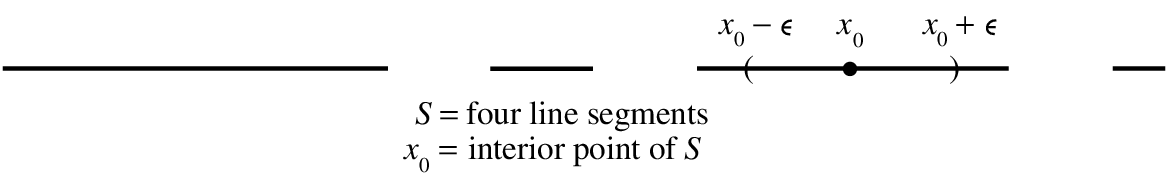
\includegraphics[width=3.875in,height=.6in]{png/fig010302.png}
\end{center}
\vskip6pt
\refstepcounter{figure}
\centerline{\bf Figure \thefigure} \label{figure:1.3.2}
\vskip12pt

The idea of neighborhood is fundamental and occurs in many other
contexts, some of which we will see later in this book. Whatever the
context, the idea is the same: some definition of ``closeness'' is
given (for example, two real numbers are ``close'' if their difference
is ``small''), and a neighborhood of a point $x_0$ is a set that
contains all points sufficiently close to $x_0$.

\begin{example}\label{example:1.3.4}\rm   \rm
An open interval $(a,b)$ is an open set, because if $x_0\in (a,b)$ and
$\epsilon\le\min\{x_0-a,b-x_0\}$, then
$$
(x_0-\epsilon, x_0+\epsilon )\subset (a,b).
$$
The entire line $\R=(-\infty,\infty)$ is open, and therefore
$\emptyset\,(=\R^c)$ is closed. However, $\emptyset$ is also
open, for to deny this is to say that $\emptyset $ contains a point
that is
not an interior point, which is absurd because $\emptyset$ contains no
points. Since $\emptyset$ is open, $\R\,(=\emptyset^c)$ is
closed.
Thus, $\R$ and $\emptyset$ are both open and closed. They are
the only subsets of $\R$ with this property
(Exercise~\ref{exer:1.3.18}).
\bbox\end{example}

A {\it deleted neighborhood\/}
 of a point
$x_0$ is a set that contains
every point of some neighborhood of $x_0$ except for $x_0$ itself. For
example,
$$
S=\set{x}{0<|x-x_0|<\epsilon}
$$
is a deleted neighborhood of $x_0$. We also say that it is a {\it
deleted
$\epsilon$-neighborhood} of
$x_0$.

\begin{theorem}\label{thmtype:1.3.3}\mbox{}
\begin{alist}
\item % (a)
  The union of open sets is open$.$
\item % (b)
 The intersection of closed sets is closed$.$
\end{alist}
These statements apply to
arbitrary collections, finite or infinite, of open and closed
sets$.$
\end{theorem}

\proof
\part{a}  Let ${\mathcal G}$ be a collection of open sets and
$$
S=\cup\set{G}{G\in {\mathcal G}}.
$$
If $x_0\in S$, then $x_0\in G_0$ for some $G_0$ in ${\mathcal G}$, and
since $G_0$ is open, it contains some $\epsilon$-neighborhood of
$x_0$. Since $G_0\subset S$, this $\epsilon$-neighborhood is in $S$,
which is consequently a neighborhood of $x_0$. Thus, $S$ is a
neighborhood of each of its points, and therefore open, by definition.

\part{b} Let ${\mathcal F}$ be a collection of closed sets and $T
=\cap\set{F}{F\in {\mathcal F}}$. Then $T^c=\cup\set{F^c}{F\in {\mathcal
F}}$
(Exercise~\ref{exer:1.3.7}) and, since each $F^c$ is open,
$T^c$ is open, from \part{a}. Therefore, $T$ is closed, by
definition.
\bbox

\begin{example}\label{example:1.3.5}\rm   If
$-\infty<a<b<\infty$, the set
$$
[a,b]=\set{x}{a\le x\le b}
$$
is closed, since its complement is the union of the open sets
$(-\infty,a)$ and $(b,\infty)$. We say that $[a,b]$ is a {\it closed
interval}. The set
$$
[a,b)=\set{x}{a\le x<b}
$$
is a {\it half-closed\/} or {\it half-open interval\/}
if $-\infty<a<b<
\infty$, as is
$$
(a,b]=\set{x}{a<x\le b};
$$
however, neither of these sets is open or closed.  (Why not?)  {\it
Semi-infinite closed intervals} are
sets of the form
$$
[a,\infty)=\set{x}{a\le x}\mbox{\quad and\quad}
(-\infty,a]=\set{x}{x\le a},
$$
where $a$ is finite. They are closed sets, since their complements
are the open intervals $(-\infty,a)$ and $(a,\infty)$, respectively.
\bbox\end{example}

Example~\ref{example:1.3.4} shows that a set may be both open and closed,
and Example~\ref{example:1.3.5} shows that a set may be neither. Thus,
open and closed are not opposites in this context, as they are in
everyday speech.

\begin{example}\label{example:1.3.6}\rm From
Theorem~\ref{thmtype:1.3.3} and
Example~\ref{example:1.3.4}, the union of any collection of open intervals
is an open set. (In fact, it can be shown that every nonempty open
subset of $\R$ is the union of open intervals.) From
Theorem~\ref{thmtype:1.3.3} and Example~\ref{example:1.3.5}, the intersection
of any collection of closed intervals is closed.
\bbox\end{example}

It can be shown that the intersection of finitely many open sets is
open, and that the union of finitely many closed sets is closed.
However,
the intersection of infinitely many open sets need not be open, and
the union of infinitely many closed sets need not be closed
(Exercises~\ref{exer:1.3.8} and \ref{exer:1.3.9}).

\begin{definition}\label{thmtype:1.3.4} Let $S$ be a subset of ${\mathcal
R}$. Then
\begin{alist}
\item % (a)
 $x_0$ is a {\it limit point\/}
of $S$ if every deleted neighborhood of $x_0$ contains a point of~$S$.


\item % (b)
$x_0$ is a {\it boundary point\/} of $S$ if every neighborhood
of $x_0$ contains at least one point in $S$ and one not in $S$. The set of
boundary points of $S$ is the {\it boundary\/} of $S$, denoted by $\partial
S$. The {\it closure\/} of $S$, denoted by $\overline{S}$, is
$\overline{S}=S\cup \partial S$.


\item % (c)
$x_0$ is an \emph{isolated point} of $S$ if $x_0\in S$
 and there is a neighborhood of $x_0$ that contains no other point of
$S$.

\item % (d)
$x_0$ is \emph{exterior} to $S$ if $x_0$ is in the interior of $S^c$. The
collection of such points is the {\it exterior\/} of $S$.
\end{alist}
\end{definition}

\enlargethispage{\baselineskip}
\begin{example}\label{example:1.3.7}\rm  Let
$S=(-\infty,-1]\cup (1,2)\cup
\{3\}$. Then
\newpage
\begin{alist}
\item % (a)
The set of limit points of $S$ is $(-\infty,-1]\cup
[1,2]$.
\item % (b)
$\partial S=\{-1,1,2,3\}$ and $\overline{S}=
(-\infty,-1]\cup [1,2]\cup\{3\}$.
\item % (c)
 $3$ is the only isolated point
of $S$.
\item % (d)
 The exterior of $S$ is $(-1,1)\cup (2,3)\cup (3,\infty)$.
\end{alist}
\end{example}

\begin{example}\label{example:1.3.8}\rm For $n\ge1$, let
$$
I_n=\left[\frac{1}{2n+1}, \frac{1}{2n}\right]\mbox{\quad and\quad}
S=
\bigcup^\infty_{n=1} I_n.
$$
Then
\begin{alist}
\item % (a)
The set of limit points of $S$ is $S\cup\{0\}$.
\item % (b)
$\partial S=
\set{x}{x=0 \mbox{ or } x=1/n\ (n\ge2)}$ and
$\overline{S}=S\cup\{0\}$.
\item % (c)
 $S$ has no isolated points.
\item % (d)
 The exterior of $S$ is
\end{alist}
$$
(-\infty,0)\cup\left[\bigcup^\infty_{n=1}\left(\frac{1}{2n+2},\frac{1}
{2n+1}\right)\right]\cup\left(\frac{1}{2},\infty\right).
$$
\end{example}

\begin{example}\label{example:1.3.9}\rm
Let $S$ be the set of rational numbers. Since every interval contains
a rational number (Theorem~\ref{thmtype:1.1.6}), every real
number is a limit point of $S$; thus, $\overline{S}=\R$. Since
every interval also contains an irrational number
(Theorem~\ref{thmtype:1.1.7}), every real number is a
boundary
point of $S$; thus $\partial S=\R$.
 The interior and exterior of $S$ are both empty, and $S$
has no isolated points.
$S$ is neither open nor closed.
\bbox\end{example}


The next theorem says that $S$ is closed if and only if $S=\overline{S}$
(Exercise~\ref{exer:1.3.14}).

\begin{theorem}\label{thmtype:1.3.5}   A set $S$ is closed if and only if
no point of $S^c$ is a limit point of~$S.$
\end{theorem}

\proof
Suppose that $S$ is closed and $x_0\in S^c$. Since $S^c$ is open,
there is a neighborhood of $x_0$ that is contained in $S^c$ and
therefore contains no points of $S$. Hence, $x_0$ cannot be a limit
point of $S$. For the converse, if no point of $S^c$ is a limit point
of $S$ then every point in $S^c$ must have a neighborhood contained
in $S^c$. Therefore, $S^c$ is open and $S$ is closed.
\bbox

Theorem~\ref{thmtype:1.3.5} is usually stated as follows.

\begin{corollary}\label{thmtype:1.3.6}  A set is closed if and only if it
contains all its limit points$.$
\end{corollary}

Theorem~\ref{thmtype:1.3.5} and Corollary~\ref{thmtype:1.3.6} are equivalent.
However, we stated the theorem as we did because students sometimes
incorrectly conclude from the corollary that a closed set must have
limit points. The corollary does not say this. If $S$ has no limit
points, then the set of limit points is empty and therefore contained
in $S$. Hence, a set with no limit points is closed according to the
corollary, in agreement with Theorem~\ref{thmtype:1.3.5}. For example, any
finite set is closed. More generally, $S$ is closed if there is a
$\delta>0$  such $|x-y|\ge \delta$ for every pair $\{x,y\}$ of distinct
points in $S$.
\newpage

\boxit{Open Coverings}
A collection ${\mathcal H}$ of open sets is an {\it open
covering\/} of
a set $S$ if every point in $S$ is contained in a set $H$ belonging to
${\mathcal H}$; that is, if $S\subset\cup\set{H}{H\in {\mathcal H}}$.

\vskip.5pc
\begin{example}\label{example:1.3.10}\rm   The sets
\begin{eqnarray*}
S_1\ar=[0,1],\,  S_2=\{1,2, \dots,n, \dots\},\\
S_3\ar=\left\{1,\frac{1}{2}, \dots,\frac{1}{n}, \dots\right\},
\mbox{\quad and\quad}  S_4=(0,1)
\end{eqnarray*}
 are covered by the families of open intervals
\begin{eqnarray*}
{\mathcal H}_1\ar=\left\{\left(x-\frac{1}{N}, x+\frac{1}
{N}\right)\bigg|\,
0<
x<1\right\},\mbox{\quad($N=$  positive integer),\quad}\\
{\mathcal H}_2\ar=\left\{\left(n-\frac{1}{4},
n+\frac{1}{4}\right)\bigg|\, n=
1,2, \dots\right\},\\
{\mathcal H}_3\ar=\left\{\left(\frac{1}{n+\frac{1}{2}}, \frac{1}
{n-\frac{1}
{2}}\right)\bigg|\, n=1,2, \dots\right\},\\
\noalign{\hbox{and}}\\
{\mathcal H}_4\ar=\{(0,\rho)|\, 0<\rho<1\},
\end{eqnarray*}
respectively.
\end{example}

\vskip.5pc

\begin{theorem}
[\href{http://www-history.mcs.st-and.ac.uk/Mathematicians/Heine.html}
{Heine}--\href{http://www-history.mcs.st-and.ac.uk/Mathematicians/Borel.html}
{Borel}
Theorem]\label{thmtype:1.3.7}
If ${\mathcal H}$ is an open covering of a closed and bounded subset $S$
of the real line$,$ then $S$ has an open covering $\widetilde{\mathcal
H}$ consisting of finitely many open sets belonging to ${\mathcal H}.$
\end{theorem}

\proof
 Since $S$ is bounded, it has an  infimum $\alpha$
and a supremum $\beta$, and, since $S$ is closed, $\alpha$
and $\beta$ belong to $S$ (Exercise~\ref{exer:1.3.17}). Define
$$
S_t=S\cap [\alpha,t]  \mbox{\quad for \ } t\ge\alpha,
$$
and let
$$
F=\set{t}{\alpha\le t\le\beta \mbox{\ and finitely many sets from
${\mathcal H}$ cover $S_t$}}.
$$
Since $S_\beta=S$, the theorem will be proved if we can show that
$\beta
\in F$.  To do this, we use the completeness of the reals.

Since $\alpha\in S$, $S_\alpha$ is the singleton set $\{\alpha\}$,
which is contained in some open set $H_\alpha$ from ${\mathcal H}$
because ${\mathcal H}$ covers $S$; therefore, $\alpha\in F$. Since $F$ is
nonempty and bounded above by $\beta$, it has a supremum $\gamma$.
First, we wish to show that $\gamma=\beta$. Since $\gamma\le\beta$ by
definition of $F$, it suffices to rule out the possibility that
$\gamma<\beta$. We consider two cases.

{\sc Case 1}. Suppose that $\gamma<\beta$ and $\gamma\not\in S$. Then,
since $S$ is closed, $\gamma$ is not a limit point of $S$
(Theorem~\ref{thmtype:1.3.5}). Consequently, there is an  $\epsilon>0$
such that
$$
[\gamma-\epsilon,\gamma+\epsilon]\cap S=\emptyset,
$$
so $S_{\gamma-\epsilon}=S_{\gamma+\epsilon}$. However, the
definition of $\gamma$ implies that $S_{\gamma-\epsilon}$ has a finite
subcovering from ${\mathcal H}$, while $S_{\gamma+\epsilon}$ does not.
This is a contradiction.

{\sc Case 2}. Suppose that  $\gamma<\beta$ and $\gamma\in S$. Then
there is an open
set $H_\gamma$ in ${\mathcal H}$ that contains $\gamma$ and, along with $\gamma$, an
interval $[\gamma-\epsilon,\gamma+\epsilon]$ for some positive
$\epsilon$.
Since $S_{\gamma-\epsilon}$ has a finite covering $\{H_1, \dots,H_n\}$ of
sets from ${\mathcal H}$, it follows that $S_{\gamma+\epsilon}$ has the finite
covering $\{H_1, \dots,H_n,H_\gamma\}$. This contradicts the
definition of $\gamma$.

Now we know that $\gamma=\beta$, which is in $S$. Therefore, there is
an open set $H_\beta$ in ${\mathcal H}$ that contains $\beta$ and along
with $\beta$, an interval of the form
$[\beta-\epsilon,\beta+\epsilon]$, for some positive $\epsilon$. Since
$S_{\beta-\epsilon}$ is covered by a finite collection of sets
$\{H_1, \dots,H_k\}$, $S_\beta$ is covered by the finite collection
$\{H_1, \dots, H_k, H_\beta\}$. Since $S_\beta=S$,  we are
finished.
\bbox

Henceforth, we will say that a closed and bounded set is {\it
compact\/}.
The Heine--Borel theorem says that any open covering of a compact set
$S$ contains a finite collection that also covers $S$. This theorem
and its converse (Exercise~\ref{exer:1.3.21}) show that we could just as
well define a set $S$ of reals to be compact if it has the
Heine--Borel property; that is, if every open covering of $S$ contains
a finite subcovering. The same is true of $\R^n$, which we study
in Section~5.1. This definition generalizes to more abstract
spaces (called {\it topological spaces\/})
for which the concept of boundedness need not be defined.

\begin{example}\label{example:1.3.11}\rm   \rm
Since  $S_1$ in Example~\ref{example:1.3.10} is compact,
the Heine--Borel theorem implies that $S_1$ can be covered by a finite
number of intervals from ${\mathcal H}_1$. This is easily verified, since,
for example, the $2N$ intervals from ${\mathcal H}_1$ centered at the
points $x_k=k/2N\,(0\le k\le2N-1)$ cover $S_1$.

The Heine--Borel theorem does not apply to the other sets in
Example~\ref{example:1.3.10} since they are not compact: $S_2$ is unbounded
and $S_3$ and $S_4$ are not closed, since they do not contain all
their limit points (Corollary~\ref{thmtype:1.3.6}). The conclusion of the
Heine--Borel theorem does not hold for these sets and the open
coverings that we have given for them. Each point in $S_2$ is
contained in
exactly one set from ${\mathcal H}_2$, so removing even one of these sets
leaves a point of $S_2$ uncovered. If $\widetilde{\mathcal H}_3$ is any
finite collection of sets from ${\mathcal H}_3$, then
$$
\frac{1}{n}\not\in\cup\set{H}{H\in\widetilde{\mathcal H}_3}
$$
for $n$ sufficiently large. Any finite collection
$\{(0,\rho_1), \dots,
(0,\rho_n)\}$ from ${\mathcal H}_4$ covers only the interval $(0,\rho_{\max})$,
where
$$
\rho_{\max}=\max\{\rho_1, \dots,\rho_n\}<1.
$$
\end{example}

\enlargethispage{\baselineskip}
\boxit{The Bolzano--Weierstrass Theorem}
As an application of the Heine--Borel theorem, we  prove the
following theorem of Bolzano and Weierstrass.

\begin{theorem}
[\href{http://www-history.mcs.st-and.ac.uk/Mathematicians/Bolzano.html}
{Bolzano}--\href{http://www-history.mcs.st-and.ac.uk/Mathematicians/Weierstrass.html}
{Weierstrass}
 Theorem]\label{thmtype:1.3.8}
 Every bounded infinite set of real numbers has at least one
limit point$.$
\end{theorem}

\proof
 We will show that a bounded nonempty set without a limit point
can contain only a finite number of points. If $S$ has no limit
points, then $S$ is closed (Theorem~\ref{thmtype:1.3.5}) and every point
$x$ of $S$ has an open neighborhood $N_x$ that contains no point of
$S$ other than $x$. The collection
$$
{\mathcal H}=\set{N_x}{x\in S}
$$
is an open covering for $S$. Since $S$ is also bounded,
Theorem~\ref{thmtype:1.3.7} implies that $S$ can be covered by a finite
collection of sets from ${\mathcal H}$, say $N_{x_1}$, \dots, $N_{x_n}$.
Since
these sets contain only $x_1$, \dots, $x_n$ from $S$, it follows that
$S=\{x_1, \dots,x_n\}$.
\bbox

\vskip1pc
\exercises
\begin{exerciselist}

\item\label{exer:1.3.1}
 Find $S\cap T$, $(S\cap T)^c$, $S^c\cap T^c$, $S\cup T$, $(S
\cup T)^c$, and $S^c\cup T^c$.

\hspace*{-1em}
\begin{tabular}{ll}
\part{a} $S=(0,1)$, $T=\left[\frac{1}{2}, \frac{3}{2}\right]$&
\part{b} $S=\set{x}{x^2>4}$, $T=\set{x}{x^2<9}$\\[2\jot]
\part{c} $S=(-\infty,\infty)$, $T=\emptyset$&
\part{d} $S=(-\infty,-1)$, $T=(1,\infty)$
\end{tabular}

\item\label{exer:1.3.2}
Let $S_k=(1-1/k,2+1/k]$, $k\ge1$.  Find

\hspace*{-1em}
\begin{tabular}{llll}
\part{a}  $\dst{\bigcup^\infty_{k=1}S_k}$
&\part{b} $\dst{\bigcap^\infty_{k=1}S_k}$&
\part{c}  $\dst{\bigcup^\infty_{k=1}S^c_k}$&
\part{d} $\dst{\bigcap^\infty_{k=1}S^c_k}$
\end{tabular}

\item\label{exer:1.3.3}
Prove: If $A$ and $B$ are sets and there is a set $X$ such that
 $A\cup X=B\cup X$ and $A\cap X=B\cap X$, then $A=B$.

\item\label{exer:1.3.4}
Find the largest $\epsilon$ such that $S$ contains
an $\epsilon$-neighborhood of $x_0$.

\hspace*{-1em}
\begin{tabular}{ll}
\part{a} $x_0=\frac{3}{4}$, $S=\left[\frac{1}{2},1\right)$&
\part{b} $x_0=\frac{2}{3}$, $S=\left[\frac{1}{2},
\frac{3}{2}\right]$\\[2\jot]
\part{c} $x_0=5$, $S=(-1,\infty)$&
\part{d} $x_0=1$, $S=(0,2)$
\end{tabular}

\item\label{exer:1.3.5}
 Describe the following sets as open, closed, or neither, and find
$S^0$, $(S^c)^0$, and $(S^0)^c$.

\hspace*{-1em}
\begin{tabular}{ll}
\part{a} $S=(-1,2)\cup [3,\infty)$&
\part{b} $S=(-\infty,1)\cup (2,\infty)$\\[2\jot]
\part{c} $S=[-3,-2]\cup [7,8]$&
\part{d} $S=\set{x}{x=\mbox{integer}}$
\end{tabular}

\item\label{exer:1.3.6}
 Prove that  $(S\cap T)^c=S^c\cup T^c$ and $(S\cup T)^c=S^c\cap T^c$.

\item\label{exer:1.3.7}
 Let ${\mathcal F}$ be a collection of sets and define
$$
I=\cap\set{F}{F\in {\mathcal F}}\mbox{\quad and \quad} U=\cup\set{F}{F\in
{\mathcal F}}.
$$
Prove that \part{a} $I^c=\cup\set{F^c}{F\in {\mathcal F}}$ and
\part{b} $U^c=\set{\cap F^c}{F\in {\mathcal F}}$.

\enlargethispage{\baselineskip}
\item\label{exer:1.3.8}
\begin{alist}
\item % (a)
 Show that the intersection of finitely many open sets is
open.
\newpage
\item % (b)
 Give an example showing that the intersection of infinitely many open
sets may fail to be open.
\end{alist}

\item\label{exer:1.3.9}
\begin{alist}
\item % (a)
Show that the union of finitely many closed sets is closed.
\item % (b)
 Give an example showing that the union of infinitely many closed
sets may fail to be closed.
\end{alist}

\item\label{exer:1.3.10}
Prove:
\begin{alist}
\item % (a)
  If $U$ is a neighborhood of $x_0$ and $U\subset V$,
then $V$ is a neighborhood of~$x_0$.
\item % (b)
 If $U_1$, \dots, $U_n$ are neighborhoods of $x_0$, so is
$\bigcap^n_{i=1}U_i$.
\end{alist}

\item\label{exer:1.3.11}
Find the set of limit points of $S$, $\partial S$, $\overline S$, the
set of isolated points of $S$, and the exterior of $S$.
\begin{alist}
\item % (a)
 $S=(-\infty,-2)\cup (2,3)\cup\{4\}$ $\cup (7,\infty)$
\item % (b)
  $S=\{\mbox{all integers}\}$
\item % (c)
  $S=\cup\set{(n,n+1)}{n=\mbox{integer}}$
\item % (d)
  $S=\set{x}{x=1/n, n=1,2,3, \dots}$
\end{alist}

\item\label{exer:1.3.12}
Prove:  A limit point of a set $S$ is either an interior point
or a boundary point of $S$.

\item\label{exer:1.3.13}
Prove:  An isolated point of $S$ is a boundary point of $S^c$.

\item\label{exer:1.3.14}
 Prove:
\begin{alist}
\item % (a)
 A boundary point of a set $S$ is either a limit
point or an isolated point of $S$.
\item % (b)
 A set $S$ is closed if and only if $S=\overline{S}$.
\end{alist}

\item\label{exer:1.3.15}
Prove or disprove: A set has no limit points if and only if each of
its points is isolated.

\item\label{exer:1.3.16}
\begin{alist}
\item % (a)
 Prove:  If $S$ is bounded above and $\beta=\sup S$,
 then $\beta\in\partial S$.
\item % (b)
 State the analogous result for a set bounded below.
\end{alist}

\item\label{exer:1.3.17}
 Prove:  If $S$ is closed and bounded, then $\inf S$
and $\sup S$ are both in $S$.

\item\label{exer:1.3.18}
 If a nonempty subset $S$ of $\R$ is both open and closed,
then $S=\R$.

\item\label{exer:1.3.19}
Let $S$ be an arbitrary set. Prove:
 \part{a} $\partial S$ is closed.
\part{b} $S^0$ is open.
\part{c} The exterior of $S$ is open.
 \part{d}
The limit points of $S$ form a closed set. \part{e}
$\overline{\left(\overline{S}\right)}=\overline{S}$.
\item\label{exer:1.3.20}
 Give counterexamples to the following false statements.
\begin{alist}
\item % (a)
 The isolated points of a set form a closed set.
\item % (b)
 Every open set contains at least two points.
\item % (c)
 If $S_1$ and $S_2$ are arbitrary sets, then $\partial (S_1
\cup S_2)=\partial S_1\cup\partial S_2$.
\item % (d)
 If $S_1$ and $S_2$ are arbitrary sets, then $\partial (S_1
\cap S_2)=\partial S_1\cap\partial S_2$.
\item % (e)
 The supremum of a bounded nonempty set is the
greatest of its limit points.
\item % (f)
 If $S$ is any set, then $\partial (\partial S)=\partial
S$.
\item % (g)
 If $S$ is any set, then $\partial\overline{S}=\partial
S$.
\item % (h)
 If $S_1$ and $S_2$ are arbitrary sets, then $(S_1\cup
S_2)^0=S^0_1\cup S^0_2$.
\end{alist}

\item\label{exer:1.3.21}
Let $S$ be a nonempty subset of $\R$ such that if ${\mathcal H}$ is
any open covering of $S$, then $S$ has an open covering
$\widetilde{{\mathcal
H}}$ comprised of finitely many open sets from ${\mathcal H}$. Show that
$S$ is compact.

\item\label{exer:1.3.22}
  A set $S$ is. in a set
$T$ if
$S\subset T\subset
\overline{S}$.
\begin{alist}
\item % (a)
Prove: If $S$ and $T$ are sets of real numbers and $S\subset T$, then
$S$ is dense in $T$ if and only if every neighborhood of each point in
$T$ contains a point from $S$.
\item % (b)
State how \part{a} shows that the definition given
here is consistent with the restricted definition of a dense subset of
the reals given in Section~1.1.
\end{alist}

\item\label{exer:1.3.23} Prove:

\begin{tabular}[t]{@{}p{168pt}@{}p{168pt}}
\part{a} $(S_1\cap S_2)^0=S^0_1\cap S^0_2$&\part{b} $S^0_1
\cup S^0_2\subset (S_1\cup S_2)^0$
\end{tabular}

\item\label{exer:1.3.24}
Prove:

\begin{tabular}[t]{@{}p{168pt}@{}p{168pt}}
\part{a} $\partial(S_1\cup S_2)\subset\partial S_1\cup\partial
S_2$&\part{b} $\partial (S_1\cap S_2)\subset\partial S_1\cup
\partial S_2$\\[2\jot]
\part{c} $\partial\overline{S}\subset\partial S$&\part{d}
$\partial S=\partial S^c$\\[2\jot]
\part{e} $\partial (S-T)\subset\partial S\cup\partial T$
\end{tabular}

\label{sectionend:\thesection}
\end{exerciselist}

\newpage  %Chapter 2
\pdfbookmark[0]{Chapter 2 Differential Calculus of Functions of One Variable}{chapter:2}
\setcounter{chapter}{2}
\setcounter{section}{0}
\setcounter{page}{30}
\thispagestyle{plain}
\vspace*{-2pt}
\chaptertitle{
Differential Calculus of\\\vskip6pt Functions of
One  Variable}

\noindent
IN THIS CHAPTER
we study  the differential calculus of functions of one
variable.

\noindent
 SECTION~2.1  introduces the concept of function and discusses
arithmetic operations
on functions, limits, one-sided limits, limits at $\pm\infty$,
and monotonic functions.

\noindent
SECTION~2.2  defines  continuity and discusses removable
discontinuities,
composite functions, bounded functions, the intermediate value
theorem, uniform continuity, and additional properties of monotonic
functions.

\noindent
SECTION~2.3 introduces  the derivative and its
geometric interpretation. Topics covered include the interchange of
differentiation and arithmetic operations, the chain rule, one-sided
derivatives, extreme values of a differentiable function, Rolle's
theorem, the intermediate value theorem for derivatives, and the mean
value theorem and its consequences.

\noindent
SECTION~2.4 presents a comprehensive discussion of L'Hospital's rule.

\noindent
SECTION~2.5 discusses the approximation of a function $f$ by
the Taylor polynomials of $f$ and applies this result to locating
local extrema of $f$.  The section concludes with the extended mean
value theorem, which implies Taylor's theorem.

\pagestyle{myheadings}
\newsection{1}{Differential Calculus of Functions of One
Variable}{Functions and Limits}
\vskip14pt

\subpdfbookmark{Section 2.1 Functions and Limits}{section:2.1}
\renewcommand{\thissection}{\sectiontitle{FUNCTIONS AND LIMITS}}
\thissection
\noindent
In this section we study limits of real-valued functions of a real
variable. You studied limits in
calculus. However,
we will look more carefully at the definition of limit and prove
theorems usually not proved in calculus.

A rule $f$ that assigns to each member of a nonempty set $D$ a unique
member of a set $Y$ is  a {\it function from $D$ to
$Y$\/}.
We write the relationship between a member $x$ of $D$ and the
member $y$ of $Y$ that $f$ assigns to $x$ as
$$
y=f(x).
$$
The set $D$ is the {\it domain\/}  of
$f$, denoted by
$D_f$. The members of $Y$ are the possible {\it
values\/} of
$f$.
 If $y_0\in Y$ and there is an
$x_0$ in $D$ such that $f(x_0)=y_0$ then we say that $f$
{\it attains\/}
\enlargethispage{.2in}

\newpage
\noindent
or {\it assumes\/} the value $y_0$. The set of values attained by $f$ is
the {\it range\/} of
$f$. A
{\it real-valued function of a real
variable} is a
function whose domain and range are both subsets of the
reals. Although we are concerned only with real-valued functions of a
real variable in this section,  our definitions are not
restricted to this situation. In later sections we will consider
situations where the range or domain, or both, are
subsets of vector spaces.

\begin{example}\label{example:2.1.1}\rm
The functions $f$, $g$, and $h$ defined on $(-\infty,\infty)$ by
$$
f(x)=x^2,\quad g(x)=\sin x,\mbox{\quad and \quad} h(x)=e^x
$$
have ranges $[0,\infty)$, $[-1,1]$, and $(0,\infty)$, respectively.
\end{example}

\begin{example}\label{example:2.1.2}\rm   The equation
\begin{equation}\label{eq:2.1.1}
[f(x)]^2=x
\end{equation} does not define a function except on the singleton set
$\{0\}$. If $x<0$, no real number satisfies \eqref{eq:2.1.1}, while if
$x>0$, two real numbers satisfy \eqref{eq:2.1.1}. However, the conditions
$$
[f(x)]^2=x\mbox{\quad and \quad} f(x)\ge0
$$
define a function $f$ on $D_f=[0,\infty)$ with values
$f(x)=\sqrt{x}$.
Similarly, the conditions
$$
[g(x)]^2=x\mbox{\quad and \quad} g(x)\le0
$$
define a function $g$ on $D_g=[0,\infty)$ with values
$g(x)=-\sqrt{x}$.
The ranges of $f$ and $g$ are $[0,\infty)$ and $(-\infty,0]$, respectively.
\bbox\end{example}

\samepage{
It is important to understand that the definition of a function
includes the specification of its domain and that there is a
difference between $f$, the {\it name\/} of the function, and $f(x)$,
the {\it value\/} of $f$ at $x$. However, strict observance of these
points
leads to annoying verbosity, such as ``the function $f$ with domain
$(-\infty,\infty)$ and values $f(x)=x$.'' We will avoid this in two
ways: (1) by agreeing that if a function $f$ is introduced without
explicitly defining $D_f$, then $D_f$ will be understood to consist
of all points $x$ for which the rule defining $f(x)$ makes sense, and
(2) by bearing in mind the distinction between $f$ and $f(x)$, but
not emphasizing it when it would be a nuisance to do so. For example,
we will write ``consider the function $f(x)=\sqrt{1-x^2}$,'' rather
than ``consider the function $f$ defined on $[-1,1]$ by
$f(x)=\sqrt{1-x^2}$,'' or ``consider the function $g(x)=1/\sin x$,''
rather than ``consider the function $g$ defined for $x\ne k\pi$
($k=$ integer) by $g(x)=1/\sin x$.'' We will also write $f=c$
(constant) to denote the function $f$ defined by $f(x)=c$ for all $x$.

Our definition of function is somewhat intuitive, but adequate for our
purposes. Moreover, it is the working form of the definition, even
if the idea is introduced more rigorously to begin with. For a more
precise definition, we first define the
\href{http://www-history.mcs.st-and.ac.uk/Mathematicians/Descartes.html}
{\it Cartesian\/}
{\it product\/}
$X \times Y$ of two nonempty sets $X$ and $Y$ to be the set of all
ordered pairs $(x,y)$ such that $x\in X$ and $y\in Y$; thus,
$$
X\times Y=\set{(x,y)}{x\in X, y\in Y}.
$$}

\newpage
\noindent
A nonempty subset $f$ of $X\times Y$ is  a {\it
function\/}
if no $x$ in $X$ occurs more than once as a first member among the
elements of $f$. Put another way,  if $(x,y)$ and
$(x,y_1)$ are in $f$, then $y=y_1$. The set of $x$'s that occur as
first members of $f$ is  the
 of
$f$. If
$x$ is in
the domain of $f$, then the unique $y$ in $Y$ such that $(x,y)\in f$
is  the {\it value of $f$ at $x$\/},
 and we write
$y=f(x)$. The
set of all such values, a subset of $Y$, is the {\it range of $f$\/}.

\boxit{Arithmetic Operations on Functions}
\vspace*{-4ex}
\begin{definition}\label{thmtype:2.1.1}
If  $D_f\cap D_g\ne
\emptyset,$  then $f+g,$ $f-g,$ and $fg$ are defined on
$D_f\cap D_g$ by
\begin{eqnarray*}
(f+g)(x)\ar= f(x)+g(x),\\
(f-g)(x)\ar= f(x)-g(x),\\
\noalign{\hbox{and}}
(fg)(x)\ar= f(x)g(x).
\end{eqnarray*}
The quotient $f/g$ is defined by
$$
\left(\frac{f}{ g}\right) (x)=\frac{f(x)}{ g(x)}
$$
for $x$ in $D_f\cap D_g$ such that $g(x)\ne0.$
\end{definition}

\begin{example}\label{example:2.1.3}\rm
If $f(x)=\sqrt{4-x^2}$ and $g(x)=\sqrt{x-1},$ then $D_f=[-2,2]$ and
$D_g=[1,\infty),$ so  $f+g,$ $f-g,$ and $fg$ are defined on $D_f
\cap D_g=[1,2]$ by
\begin{eqnarray*}
(f+g)(x)\ar= \sqrt{4-x^2}+\sqrt{x-1},\\
(f-g)(x)\ar= \sqrt{4-x^2}-\sqrt{x-1},
\end{eqnarray*}
and
\begin{equation}\label{eq:2.1.2}
(fg)(x)=(\sqrt{4-x^2})(\sqrt{x-1})=
\sqrt{(4-x^2)(x-1)}.
\end{equation}
The quotient $f/g$ is defined on $(1,2]$ by
$$
\left(\frac{f}{ g}\right)(x)=\sqrt{\frac{4-x^2}{x-1}}.
$$
Although the last expression in \eqref{eq:2.1.2} is also
defined for $-\infty<x<-2,$ it does not represent $fg$ for such $x,$
since $f$ and $g$ are not defined on $(-\infty,-2]$.
\end{example}

\enlargethispage{\baselineskip}
\begin{example}\label{example:2.1.4}\rm
If $c$ is a real number, the function $cf$ defined by $(cf)(x)=cf(x)$
can be regarded as the product of $f$ and a constant function. Its
domain is $D_f$. The sum and product of $n\,(\ge2)$ functions
$f_1$, \dots, $f_n$ are defined by
$$
(f_1+f_2+\cdots+f_n)(x)=f_1(x)+f_2(x)+\cdots+f_n(x)
$$

\newpage
\noindent
and
\begin{equation}\label{eq:2.1.3}
(f_1f_2\cdots f_n)(x)=f_1(x) f_2(x)\cdots f_n(x)
\end{equation}
on $D=\bigcap^n_{i=1} D_{f_i}$, provided that $D$ is nonempty. If
$f_1=f_2
=\cdots=f_n$, then \eqref{eq:2.1.3} defines the $n$th {\it power of\/}
$f$:
$$
(f^n)(x)=(f(x))^n.
$$
From these definitions, we can build
the set of all {\it polynomials\/}
$$
p(x)=a_0+a_1x+\cdots+a_nx^n,
$$
starting from the constant functions and $f(x)=x$.  The
quotient
of two polynomials is a {\it rational
function\/}
$$
r(x)=\frac{a_0+a_1x+\cdots+a_nx^n}{ b_0+b_1x+\cdots+b_mx^m}\quad
(b_m\ne0).
$$
The domain of $r$ is the set of points where the denominator is
nonzero.
\end{example}

\boxit{Limits}
The essence of the concept of limit for real-valued functions of a
real variable is this: If $L$ is a real number, then $\lim_{x\to
x_0}f(x)=L$
 means that the value
$f(x)$ can be made as close to $L$ as we wish by taking $x$
sufficiently close to $x_0$. This is made precise in the following
definition.

 \vspace*{12pt}
\begin{center}
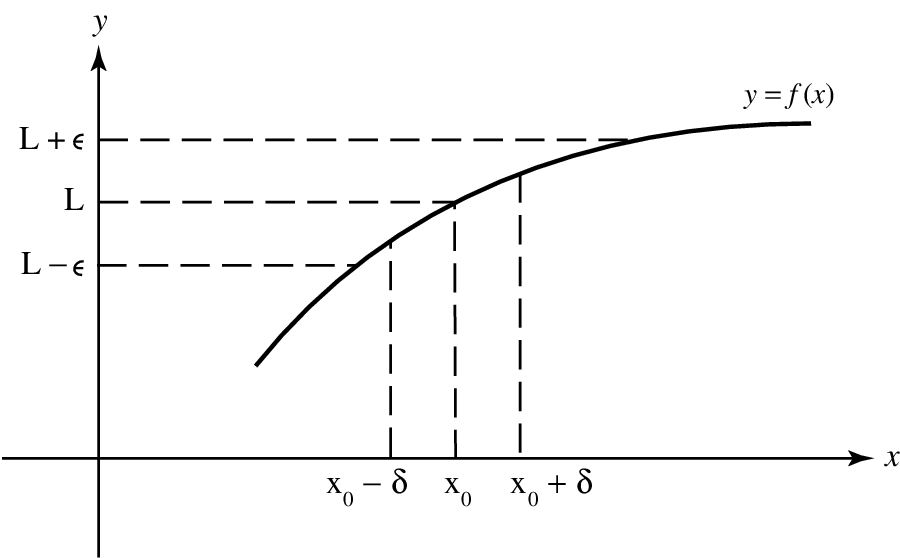
\includegraphics[width=3.2in,height=2.9in]{png/fig020101.png}
\end{center}
 \vskip6pt
 \refstepcounter{figure}
 \centerline{\bf Figure \thefigure} \label{figure:2.1.1}
 \vskip12pt

\begin{definition}\label{thmtype:2.1.2}
 We say that $f(x)$ {\it approaches the limit $L$ as $x$ approaches\/}
$x_0$, and write
$$
\lim_{x\to x_0} f(x)=L,
$$
if $f$ is defined on some deleted neighborhood of $x_0$ and, for
every $\epsilon>0$, there is a $\delta>0$ such that
\begin{equation}\label{eq:2.1.4}
|f(x)-L|<\epsilon
\end{equation}
if
\begin{equation}\label{eq:2.1.5}
0<|x-x_0|<\delta.
\end{equation}
Figure~\ref{figure:2.1.1}   depicts the graph
of a function for which
$\lim_{x
\to x_0}f(x)$ exists.
\end{definition}

\enlargethispage{\baselineskip}
\begin{example}\label{example:2.1.5}\rm
If $c$ and $x$ are arbitrary real numbers and $f(x)=cx$, then
$$
\lim_{x\to x_0} f(x)=cx_0.
$$
To prove this, we write
$$
|f(x)-cx_0|=|cx-cx_0|=|c| |x-x_0|.
$$
If $c\ne0$, this yields
\begin{equation}\label{eq:2.1.6}
|f(x)-cx_0|<\epsilon
\end{equation}
if
$$
|x-x_0|<\delta,
$$
where $\delta$ is any number such that $0<\delta\le\epsilon/|c|$. If
$c=0$, then $f(x)-cx_0=0$ for all $x$, so \eqref{eq:2.1.6} holds for all
$x$.
\bbox\end{example}

We emphasize that Definition~\ref{thmtype:2.1.2} does not involve
$f(x_0)$, or even require that it be defined, since \eqref{eq:2.1.5}
excludes the case where $x=x_0$.

\begin{example}\label{example:2.1.6}\rm   If
$$
f(x)=x\sin \frac{1}{ x},\quad x\ne0,
$$
then
$$\lim_{x\to 0}f(x)=0
$$
even though $f$ is not defined at $x_0=0$, because if
$$
0<|x|<\delta=\epsilon,
$$
then
$$
|f(x)-0|=\left| x\sin \frac{1}{ x}\right|\le |x|<\epsilon.
$$
 On the other hand, the function
$$
g(x)=\sin \frac{1}{ x},\quad x\ne0,
$$
has no limit as $x$ approaches $0$, since it assumes all values between
$-1$ and $1$ in every neighborhood of the origin
(Exercise~\ref{exer:2.1.26}).
\bbox\end{example}

\newpage
The next theorem says that a function cannot have more than one limit
at a point.

\begin{theorem}\label{thmtype:2.1.3} If $\lim_{x\to x_0} f(x)$ exists$,$
then it is unique$\,;$ that is$,$ if
\begin{equation} \label{eq:2.1.7}
\lim_{x\to x_0} f(x)=L_1\mbox{\quad and \quad}\lim_{x\to x_0} f(x)=
L_2,
\end{equation}
then $L_1=L_2.$
\end{theorem}

\proof
Suppose that  \eqref{eq:2.1.7} holds and let $\epsilon>0$.
From Definition~\ref{thmtype:2.1.2}, there are
positive numbers $\delta_1$ and $\delta_2$ such that
$$
|f(x)-L_i|<\epsilon\mbox{\quad if \quad} 0<|x-x_0|<\delta_i,
\quad i=1,2.
$$
If $\delta=\min(\delta_1,\delta_2)$, then
\begin{eqnarray*}
|L_1-L_2|\ar= |L_1-f(x)+f(x)-L_2|\\
\ar \le|L_1-f(x)|+|f(x)-L_2|<2\epsilon
\mbox{\quad if \quad} 0<|x-x_0|<\delta.
\end{eqnarray*}
We have now established an inequality that does not depend on $x$;
that is,
$$
|L_1-L_2|<2\epsilon.
$$
Since this  holds for any positive $\epsilon$,
 $L_1=L_2$.
\bbox

Definition~\ref{thmtype:2.1.2} is not changed by replacing \eqref{eq:2.1.4}
with
\begin{equation}\label{eq:2.1.8}
|f(x)-L|<K\epsilon,
\end{equation}
where $K$ is a positive constant, because if either of \eqref{eq:2.1.4} or
\eqref{eq:2.1.8} can be made to hold for any $\epsilon>0$ by making
$|x-x_0|$ sufficiently small and positive, then so can the other
(Exercise~\ref{exer:2.1.5}). This may seem to be a minor point, but it is
often convenient to work with \eqref{eq:2.1.8} rather than \eqref{eq:2.1.4},
as we will see in the proof of the following theorem.

\boxit{A Useful Theorem about Limits}
\helpbox
\begin{theorem}\label{thmtype:2.1.4} If
\begin{equation}\label{eq:2.1.9}
\lim_{x\to x_0} f(x)=L_1\mbox{\quad and \quad}\lim_{x\to x_0} g(x)=
L_2,
\end{equation}
then
\begin{eqnarray}
\lim_{x\to x_0} (f+g)(x)\ar= L_1+L_2,\label{eq:2.1.10}\\
\lim_{x\to x_0} (f-g)(x)\ar= L_1-L_2,\label{eq:2.1.11}\\
\lim_{x\to x_0} (fg)(x)\ar= L_1L_2,\label{eq:2.1.12}\\
\arraytext{and, if $L_2\ne0$,}\\
\lim_{x\to x_0}\left(\frac{f}{g}\right)(x)\ar= \frac{L_1}{
L_2}.\label{eq:2.1.13}
\end{eqnarray}
\end{theorem}

\newpage
\enlargethispage{\baselineskip}
\proof
From \eqref{eq:2.1.9} and Definition~\ref{thmtype:2.1.2},
 if $\epsilon>0$, there is a
$\delta_1>0$ such that
\begin{equation}\label{eq:2.1.14}
|f(x)-L_1|<\epsilon
\end{equation}
if $0<|x-x_0|<\delta_1$, and a $\delta_2>0$ such that
\begin{equation}\label{eq:2.1.15}
|g(x)-L_2|<\epsilon
\end{equation}
if $0<|x-x_0|<\delta_2$.  Suppose that
\begin{equation}\label{eq:2.1.16}
0<|x-x_0|<\delta=\min (\delta_1,\delta_2),
\end{equation}
so that \eqref{eq:2.1.14} and \eqref{eq:2.1.15} both hold.  Then
\begin{eqnarray*}
|(f\pm g)(x)-(L_1\pm L_2)|\ar= |(f(x)-L_1)\pm
(g(x)-L_2)|\\
\ar \le|f(x)-L_1|+|g(x)-L_2|<2\epsilon,
\end{eqnarray*}
which proves \eqref{eq:2.1.10} and \eqref{eq:2.1.11}.

To prove \eqref{eq:2.1.12}, we assume \eqref{eq:2.1.16} and write
\begin{eqnarray*}
|(fg)(x)-L_1L_2|\ar= |f(x)g(x)-L_1L_2|\\[.5\jot]
\ar= |f(x)(g(x)-L_2)+L_2(f(x)-L_1)|\\[.5\jot]
\ar \le|f(x)||g(x)-L_2|+|L_2||f(x)-L_1|\\[.5\jot]
\ar \le(|f(x)|+|L_2|)\epsilon\mbox{\quad (from \eqref{eq:2.1.14} and
\eqref{eq:2.1.15})}\\[.5\jot]
\ar \le(|f(x)-L_1|+|L_1|+|L_2|)\epsilon\\[.5\jot]
\ar \le(\epsilon+|L_1|+|L_2|)\epsilon\mbox{\quad from
\eqref{eq:2.1.14}}\\[.5\jot]
\ar \le (1+|L_1|+|L_2|)\epsilon
\end{eqnarray*}
if $\epsilon<1$
and $x$ satisfies \eqref{eq:2.1.16}.  This proves
\eqref{eq:2.1.12}.

To prove \eqref{eq:2.1.13}, we first observe that if $L_2\ne0$, there is
a $\delta_3>0$ such that
$$
|g(x)-L_2|<\frac{|L_2|}{2},
$$
so
\begin{equation} \label{eq:2.1.17}
|g(x)|>\frac{|L_2|}{2}
\end{equation}
if
$$
0<|x-x_0|<\delta_3.
$$
To see this, let $L=L_2$ and $\epsilon=|L_2|/2$ in
\eqref{eq:2.1.4}. Now suppose that
$$
0<|x-x_0|<\min
(\delta_1,\delta_2,\delta_3),
$$
\nopagebreak
 so that \eqref{eq:2.1.14}, \eqref{eq:2.1.15},
and \eqref{eq:2.1.17} all hold. Then

\pagebreak
\begin{eqnarray*}
\left|\left(\frac{f}{ g}\right)(x)-\frac{L_1}{ L_2}\right|
\ar= \left|\frac{f(x)}{ g(x)}-\frac{L_1}{ L_2}\right|\\
\ar= \frac{|L_2f(x)-L_1g(x)|}{|g(x)L_2|}\\
\ar \le\frac{2}{ |L_2|^2}|L_2f(x)-L_1g(x)|\\
\ar= \frac{2}{ |L_2|^2}\left|L_2[f(x)-L_1]+
L_1[L_2-g(x)]\right|\mbox{\quad (from \eqref{eq:2.1.17})}\\
\ar \le\frac{2}{ |L_2|^2}\left[|L_2||f(x)-L_1|+|L_1|
|L_2-g(x)|\right]\\
\ar \le\frac{2}{ |L_2|^2}(|L_2|+|L_1|)\epsilon
\mbox{\quad (from \eqref{eq:2.1.14} and \eqref{eq:2.1.15})}.
\end{eqnarray*}
This proves \eqref{eq:2.1.13}.
\bbox

Successive applications of the various parts of
Theorem~\ref{thmtype:2.1.4} permit us to find limits without the
$\epsilon$--$\delta$ arguments required by
Definition~\ref{thmtype:2.1.2}.

\begin{example}\label{example:2.1.7}\rm
Use Theorem~\ref{thmtype:2.1.4} to find
$$
\lim_{x\to2}\frac{9-x^2}{x+1}\mbox{\quad and \quad}
\lim_{x\to2}(9-x^2)(x+1).
$$

\solution
If $c$ is a constant, then $\lim_{x\to x_0} c=c$, and, from
Example~\ref{example:2.1.5}, $\lim_{x\to x_0} x=x_0$. Therefore, from
Theorem~\ref{thmtype:2.1.4},
\begin{eqnarray*}
\lim_{x\to 2} (9-x^2)\ar= \lim_{x\to 2} 9-\lim_{x\to 2} x^2\\
\ar= \lim_{x\to 2} 9-(\lim_{x\to 2} x)^2\\\ar= 9-2^2=5,
\end{eqnarray*}
and
$$
\lim_{x\to 2}(x+1)=\lim_{x\to 2}x+\lim_{x\to 2}1=2+1=3.
$$
Therefore,
$$
\lim_{x\to 2} \frac{9-x^2}{x+1}=\frac{\dst\lim_{x\to
2}(9-x^2)}{\dst\lim_{x\to2} (x+1)}=\frac{5}{3}
$$
and
$$
\lim_{x\to 2} (9-x^2)(x+1)=\lim_{x\to 2} (9-x^2)\lim_{x\to 2}(x+1)=
5\cdot3=15.
\eqno{\bbox}
$$
\end{example}

\enlargethispage{\baselineskip}
\enlargethispage{\baselineskip}
\boxit{One-Sided Limits}

\hskip-.2em
The function
$$
f(x)=2x\,\sin\sqrt{x}
$$

\newpage
\noindent satisfies the inequality
$$
|f(x)|<\epsilon
$$
if $0<x<\delta=\epsilon/2$. However, this does not mean that $\lim_{x
\to 0} f(x)=0$, since $f$ is not defined for negative $x$, as it must
be to satisfy the conditions of Definition~\ref{thmtype:2.1.2} with
$x_0=0$ and $L=0$. The function
$$
g(x)=x+\frac{|x|}{ x},\quad x\ne0,
$$
can be rewritten as
$$
g(x)=\left\{\casespace\begin{array}{ll} x+1,&x>0,\\
x-1,&x<0;\end{array}\right.
$$
hence, every open interval containing $x_0=0$ also contains points $x_1$
and $x_2$ such that $|g(x_1)-g(x_2)|$ is as close to $2$ as we
please. Therefore,  $\lim_{x\to x_0} g(x)$ does not exist
(Exercise~\ref{exer:2.1.26}).

Although $f(x)$ and $g(x)$  do not approach limits as $x$ approaches
zero, they each exhibit a definite sort of limiting behavior for small
positive values of $x$, as does $g(x)$ for small negative values of $x$.
The kind of behavior we have in mind  is defined precisely as follows.

 \vspace*{12pt}
\begin{center}
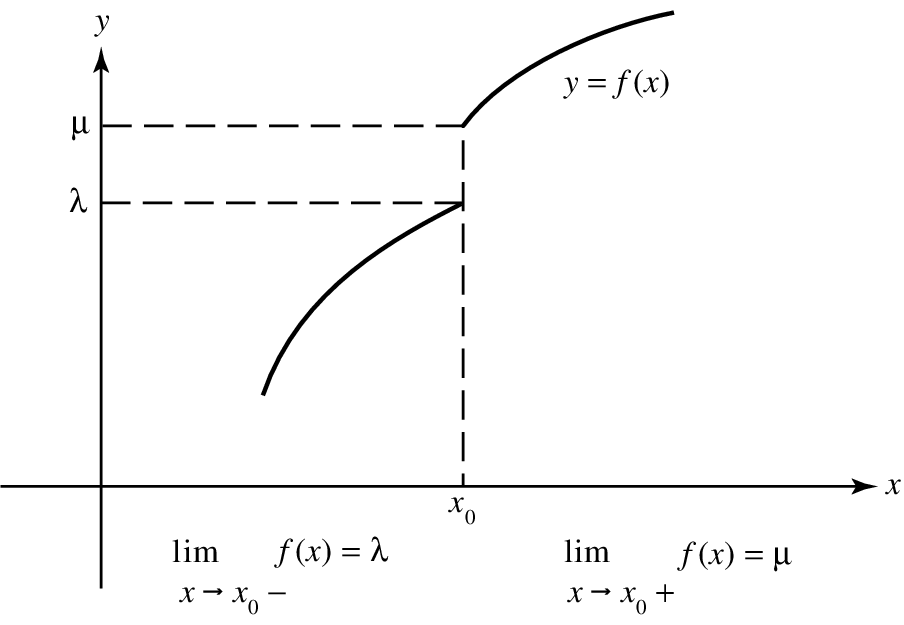
\includegraphics[width=3.1in,height=2.1in]{png/fig020102.png}
\end{center}
 \vskip6pt
 \refstepcounter{figure}
 \centerline{\bf Figure \thefigure} \label{figure:2.1.2}
 \vskip12pt

\begin{definition}\label{thmtype:2.1.5}
\begin{alist}
\item % (a)
We say that $f(x)$ {\it approaches the left-hand limit $L$ as
$x$ approaches $x_0$ from the left\/}, and write
$$
\lim_{x\to x_0-} f(x)=L,
$$
if $f$ is defined on some open interval $(a,x_0)$ and, for each
$\epsilon>0$, there is a $\delta>0$ such that
$$
|f(x)-L|<\epsilon\mbox{\quad if \quad} x_0-\delta<x<x_0.
$$
\newpage
\item % (b)
We say that $f(x)$ {\it approaches the right-hand limit $L$ as $x$
approaches $x_0$ from the right\/}, and write
$$
\lim_{x\to x_0+} f(x)=L,
$$
if $f$ is defined on some open interval $(x_0,b)$ and, for each
$\epsilon>0$, there is a $\delta>0$ such that
$$
|f(x)-L|<\epsilon\mbox{\quad if \quad} x_0<x<x_0+\delta.
\eqno{\bbox}
$$
\end{alist}
\end{definition}

Figure~\ref{figure:2.1.2} shows the graph of a function that has distinct
left- and right-hand limits at a point $x_0$.

\begin{example}\label{example:2.1.8}\rm   Let
$$
f(x)=\frac{x}{ |x|},\quad x\ne0.
$$
If $x<0$, then $f(x)=-x/x=-1$, so
$$
\lim_{x\to 0-} f(x)=-1.
$$
If $x>0$, then $f(x)=x/x=1$, so
$$
\lim_{x\to 0+} f(x)=1.
$$
\end{example}

\vspace{3pt}

\begin{example}\label{example:2.1.9}\rm   Let
$$
g(x)=\frac{x+|x|(1+x)}{ x}\sin \frac{1}{ x},\quad x\ne0.
$$
If $x<0$, then
$$
g(x)=-x\sin \frac{1}{ x},
$$
so
$$
\lim_{x\to 0-}g(x)=0,
$$
since
$$
|g(x)-0|=\left|x\sin \frac{1}{ x}\right|\le |x|<\epsilon
$$
if $-\epsilon<x<0$; that is, Definition~\ref{thmtype:2.1.5}\part{a} is
satisfied with $\delta=\epsilon$. If $x>0$, then
$$
g(x)=(2+x)\sin \frac{1}{ x},
$$
which takes on every value between $-2$ and $2$ in every interval
$(0,\delta)$. Hence, $g(x)$ does not approach a right-hand limit at
$x$ approaches $0$ from the right. This shows that a function may have
a limit from one side at a point but fail to have a limit from the
other side.
\end{example}

\begin{example}\label{example:2.1.10}\rm   We leave it to you to verify that
\begin{eqnarray*}
\lim_{x\to 0+}\left(\frac{|x|}{x}+x\right)\ar= \phantom{-}1,\\
\lim_{x\to 0-}\left(\frac{|x|}{x}+x\right)\ar= -1,\\
\lim_{x\to 0+} x\sin\sqrt{x}\ar= \phantom{-}0,
\end{eqnarray*}
and $\lim_{x\to 0-}\sin\sqrt{x}$ does not exist.
\bbox\end{example}

Left- and right-hand limits are also called {\it one-sided
limits\/}.  We will often simplify the
notation by writing
$$
\lim_{x\to x_0-} f(x)=f(x_0-)\mbox{\quad and \quad}\lim_{x\to
x_0+} f(x)=f(x_0+).
$$

The following theorem states the connection between limits and
one-sided limits. We leave the proof to you (Exercise~\ref{exer:2.1.12}).

\vspace{12pt}

\begin{theorem}\label{thmtype:2.1.6}
A function $f$ has a limit at $x_0$
if and only if it has left- and right-hand limits at $x_0,$ and they
are equal.  More specifically$,$
$$
\lim_{x\to x_0} f(x)=L
$$
if and only if
$$
f(x_0+)=f(x_0-)=L.
$$
\end{theorem}

With only minor modifications of their proofs (replacing the
inequality $0<|x-x_0|<\delta$ by $x_0-\delta<x<x_0$ or $x_0<x<x_0+
\delta$), it can be shown that the assertions of
Theorems~\ref{thmtype:2.1.3} and \ref{thmtype:2.1.4}
 remain valid if ``$\lim_{x\to x_0}$'' is replaced by ``$\lim_{x\to
x_0-}$'' or ``$\lim_{x\to x_0+}$'' throughout
(Exercise~\ref{exer:2.1.13}).

\boxit{Limits at \boldmath$\pm\infty$}
Limits and one-sided limits have to do with the behavior of a function
$f$ near a limit point of $D_f$. It is equally reasonable to study $f$
for large positive values of $x$ if $D_f$ is unbounded above or for
large negative values of $x$ if $D_f$ is unbounded below.

\vspace{12pt}

\begin{definition}\label{thmtype:2.1.7}
 We say that $f(x)$ {\it approaches
the limit $L$ as $x$ approaches\/} $\infty$,
and write
$$
\lim_{x\to\infty} f(x)=L,
$$
if $f$ is defined on an interval $(a,\infty)$ and, for each
$\epsilon>0$, there is a number $\beta$ such that
$$
|f(x)-L|<\epsilon\quad\mbox{\quad if \quad} x>\beta.
\eqno{\bbox}
$$
\end{definition}

\newpage

Figure~\ref{figure:2.1.3} provides an illustration of  the
situation described in Definition~\ref{thmtype:2.1.7}.

 \vspace*{12pt}
\begin{center}
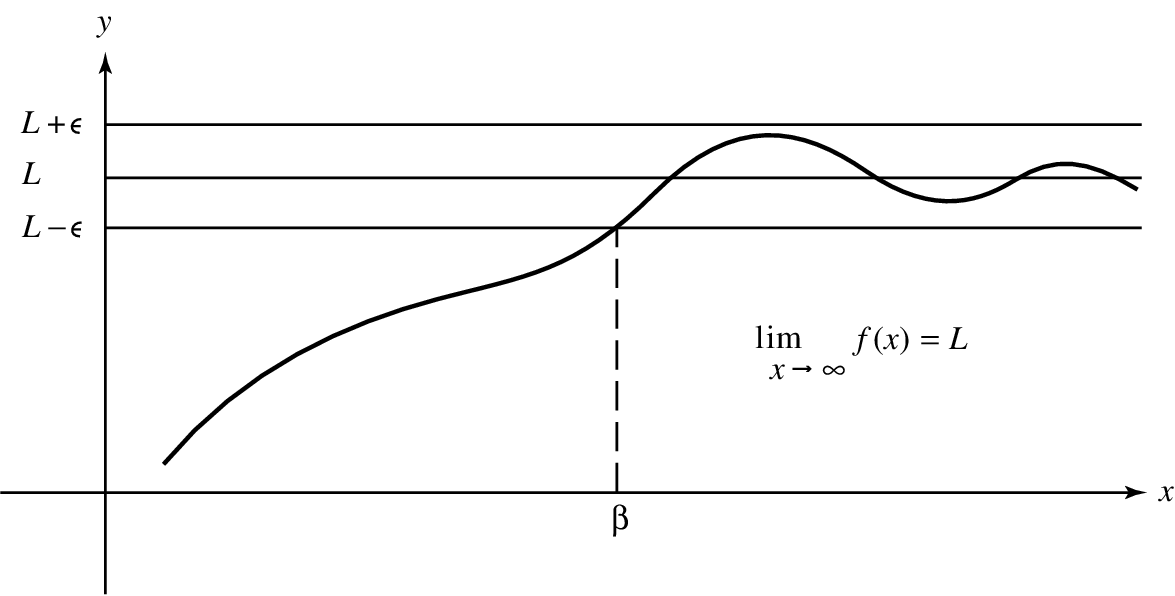
\includegraphics[width=4in,height=2.5in]{png/fig020103.png}
\end{center}
 \vskip6pt
 \refstepcounter{figure}
 \centerline{\bf Figure \thefigure} \label{figure:2.1.3}
 \vskip12pt

We leave it to you to define the statement ``$\lim_{x\to-\infty}
f(x)=L$'' (Exercise~\ref{exer:2.1.14}) and to show that
Theorems~\ref{thmtype:2.1.3} and \ref{thmtype:2.1.4}
remain valid if $x_0$ is replaced throughout by $\infty$ or $-\infty$
(Exercise~\ref{exer:2.1.16}).

\begin{example}\label{example:2.1.11}\rm   Let
$$
f(x)=1-\frac{1}{ x^2},\quad g(x)=\frac{2|x|}{1+x},\mbox{\quad and \quad}
h(x)=\sin x.
$$
Then
$$
\lim_{x\to\infty}f(x)=1,
$$
since
$$
|f(x)-1|=\frac{1}{ x^2}<\epsilon\mbox{\quad if \quad} x>
\frac{1}{\sqrt{\epsilon}},
$$
and
$$
\lim_{x\to\infty}g(x)=2,
$$
since
$$
|g(x)-2|=\left|\frac{2x}{1+x}-2\right|=\frac{2}{1+x}<\frac{2}{
x}<\epsilon\mbox{\quad if \quad} x>\frac{2}{\epsilon}.
$$
However, $\lim_{x\to\infty}h(x)$ does not exist, since $h$ assumes
all values between $-1$ and $1$ in any semi-infinite interval
$(\tau,\infty)$.

\enlargethispage{\baselineskip}
We leave it to you to show that
$\lim_{x\to-\infty}f(x)=1$, $\lim_{x\to-\infty}g(x)=-2$,
and $\lim_{x\to-\infty}h(x)$ does not exist
(Exercise~\ref{exer:2.1.17}).
\bbox\end{example}

\newpage

We will sometimes denote $\lim_{x\to\infty}f(x)$ and $\lim_{x
\to-\infty}f(x)$ by $f(\infty)$ and $f(-\infty)$,
respectively.

\boxit{Infinite Limits}
\hskip-.3em
The functions
$$
f(x)=\frac{1}{ x},\quad g(x)=\frac{1}{ x^2},\quad p(x)=\sin\frac{1}{ x},
$$
and
$$
q(x)=\frac{1}{ x^2}\sin \frac{1}{ x}
$$
do not have limits, or even one-sided limits, at $x_0=0$. They fail to
have limits in  different ways:

\begin{itemize}

\item
$f(x)$ increases beyond bound as $x$ approaches $0$ from the right
and decreases beyond bound as $x$ approaches $0$ from the left;

\item
$g(x)$ increases beyond bound as $x$ approaches zero;

\item
 $p(x)$
oscillates with ever-increasing frequency as $x$ approaches zero;

\item

$q(x)$ oscillates with
ever-increasing amplitude and frequency as $x$ approaches~$0$.
\end{itemize}

The
kind of behavior exhibited by $f$ and $g$ near $x_0=0$ is sufficiently
common and simple to lead us to define {\it infinite limits\/}.

\begin{definition}\label{thmtype:2.1.8}
We say that $f(x)$ {\it approaches $\infty$ as $x$ approaches $x_0$
from the left\/}, and write
$$
\lim_{x\to x_0-} f(x)=\infty\mbox{\quad or \quad} f(x_0-)=\infty,
$$
if $f$ is defined on an interval $(a,x_0)$ and, for each real number
$M$, there is a $\delta>0$ such that
$$
f(x)>M\mbox{\quad if \quad} x_0-\delta<x<x_0.
$$
\end{definition}

\begin{example}\label{example:2.1.12}\rm
We leave it to you to define the other kinds of infinite limits
(Exercises~\ref{exer:2.1.19} and \ref{exer:2.1.21})
 and show that
\begin{eqnarray*}
\lim_{x\to 0-}\frac{1}{x}\ar= -\infty,\quad\lim_{x\to 0+}
\frac{1}{x}=
\infty;\\
\lim_{x\to 0-}\frac{1}{ x^2}\ar= \lim_{x\to 0+} \frac{1}{
x^2}=\lim_{x\to
0} \frac{1}{ x^2}=\infty;\\
\lim_{x\to\infty}x^2\ar= \lim_{x\to-\infty}x^2=\infty;
\end{eqnarray*}
and
$$
\negthickspace\negthickspace\negthickspace\lim_{x\to\infty} x^3=
\infty,\quad\lim_{x\to-\infty} x^3=-\infty.
\eqno{\bbox}
$$
\end{example}

\newpage

Throughout this book,  ``$\lim_{x\to x_0} f(x)$ exists'' will
mean that
$$
\lim_{x\to x_0} f(x)=L,\quad \mbox{where $L$ is {\it finite\/}.}
$$
 To leave open the possibility that $L=\pm
\infty$, we will say that
$$
\lim_{x\to x_0} f(x)\quad\mbox{\it exists in the
extended
reals.\/}
$$
This convention also
applies to one-sided limits and limits as $x$ approaches $\pm\infty$.

We mentioned earlier that Theorems~\ref{thmtype:2.1.3} and \ref{thmtype:2.1.4}
remain valid if ``$\lim_{x\to x_0}$'' is replaced by ``$\lim_{x\to
x_0-}$'' or ``$\lim_{x\to x_0+}$.'' They are also valid with $x_0$
replaced by $\pm\infty$. Moreover, the counterparts of \eqref{eq:2.1.10},
\eqref{eq:2.1.11}, and \eqref{eq:2.1.12} in all  these versions of
Theorem~\ref{thmtype:2.1.4} remain valid if either or both of $L_1$ and
$L_2$ are infinite, provided that their right sides are not
indeterminate
(Exercises~\ref{exer:2.1.28} and \ref{exer:2.1.29}). Equation \eqref{eq:2.1.13}
and its
counterparts remain valid if $L_1/L_2$ is not indeterminate and
$L_2\ne0$ (Exercise~\ref{exer:2.1.30}).

\begin{example}\label{example:2.1.13}\rm
Results like Theorem~\ref{thmtype:2.1.4} yield
\begin{eqnarray*}
\lim_{x\to\infty}\sinh x\ar= \lim_{x\to\infty}\frac{e^x-e^{-x}}{2}=
\frac{1}{2}\left(\lim_{x\to\infty}e^x-\lim_{x\to\infty}e^{-x}\right)
\\
\ar= \frac{1}{2}(\infty-0)=\infty,\\
\lim_{x\to-\infty}\sinh x\ar= \lim_{x\to-\infty}\frac{e^x-e^{-x}}{2}=
\frac{1}{2}\left(\lim_{x\to-\infty}e^x-\lim_{x\to-\infty}e^{-x}\right)
\\
\ar= \frac{1}{2}(0-\infty)=-\infty,\\ \arraytext{and}\\
\lim_{x\to\infty}\frac{e^{-x}}{ x}\ar=\frac
{\dst\lim_{x\to\infty}e^{-x}}{
\dst\lim_{x\to\infty} x}=\frac{0}{\infty}=0.
\end{eqnarray*}
\end{example}

\begin{example}\label{example:2.1.14}\rm   If
$$
f(x)=e^{2x}-e^x,
$$
we cannot obtain $\lim_{x\to\infty}f(x)$ by writing
$$
\lim_{x\to\infty}f(x)=\lim_{x\to\infty}e^{2x}-\lim_{x\to
\infty}e^x,
$$
because this produces the indeterminate form $\infty-\infty$.
However, by writing
$$
f(x)=e^{2x}(1-e^{-x}),
$$
we find that
$$
\lim_{x\to\infty}f(x)= \left(\lim_{x\to\infty}e^{2x}\right)
\left(\lim_{x\to\infty}1-\lim_{x\to\infty}e^{-x}\right)
= \infty(1-0)=\infty.
$$
\end{example}

\begin{example}\label{example:2.1.15}\rm   Let
$$
g(x)=\frac{2x^2-x+1}{3x^2+2x-1}.
$$
Trying to find $\lim_{x\to\infty}g(x)$ by applying a version of
Theorem~\ref{thmtype:2.1.4} to this fraction as it is written leads to an
indeterminate form (try it!). However, by rewriting it as
$$
g(x)=\frac{2-1/x+1/x^2}{3+2/x-1/x^2},\quad x\ne0,
$$
we find that
$$
\lim_{x\to\infty}g(x)=
\frac{\dst\lim_{x\to\infty}2-\lim_{x\to\infty}1/x+
\lim_{x\to\infty} 1/x^2}{\dst\lim_{x\to\infty}
3+\lim_{x\to\infty}2/x
-\lim_{x\to\infty}1/x^2}
= \frac{2-0+0}{3+0-0}=\frac{2}{3}.
$$
\end{example}

\boxit{Monotonic Function}
\hskip-.3em
A function $f$ is {\it nondecreasing\/}
 on an interval
$I$ if
\begin{equation}\label{eq:2.1.18}
f(x_1)\le f(x_2)\quad\mbox{whenever $x_1$ and $x_2$ are in $I$ and $x_1
<x_2$},
\end{equation}
or {\it nonincreasing\/} on $I$ if
\begin{equation}\label{eq:2.1.19}
f(x_1)\ge f(x_2)\quad\mbox{whenever $x_1$ and $x_2$ are in $I$ and $x_1
<x_2$}.
\end{equation}
In either case, $f$ is  on
$I$. If
$\le$ can be
replaced by $<$ in \eqref{eq:2.1.18}, $f$ is {\it
increasing} on
$I$.
If $\ge$ can be replaced by $>$ in \eqref{eq:2.1.19}, $f$ is {\it
decreasing\/} on $I$. In either of these
two cases,
$f$ is
{\it strictly monotonic\/} on $I$.

\begin{example}\label{example:2.1.16}\rm   The function
$$
f(x)=\left\{\casespace\begin{array}{ll} x,&0\le
x<1,\\[2\jot]
 2,&1\le x\le2,\end{array}\right.
$$
is nondecreasing on $I=[0,2]$ (Figure~\ref{figure:2.1.4}), and $-f$ is
nonincreasing on $I=[0,2]$.

\begin{center}
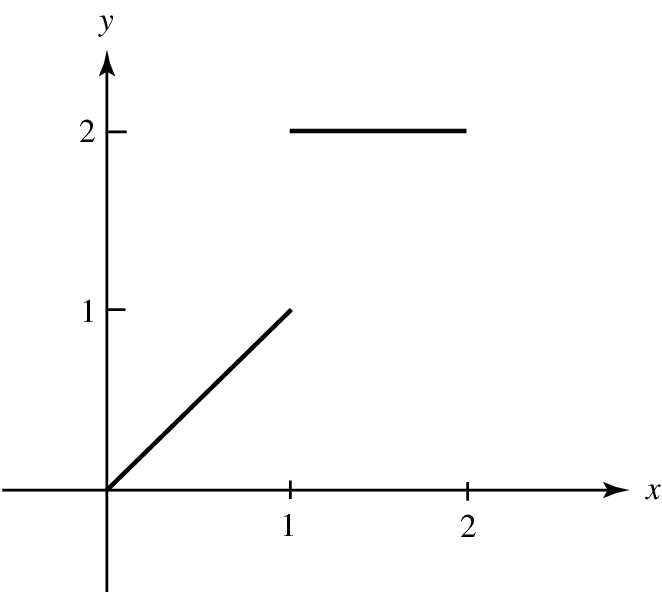
\includegraphics[width=2.35in,height=1.6in]{png/fig020104.png}
\end{center}
 \vskip6pt
 \refstepcounter{figure}
 \centerline{\bf Figure \thefigure} \label{figure:2.1.4}
%\vskip12pt

\noindent
 The function
$g(x)=x^2$
is increasing on $[0,\infty)$ (Figure~\ref{figure:2.1.5}),

 \vspace*{12pt}
\begin{center}
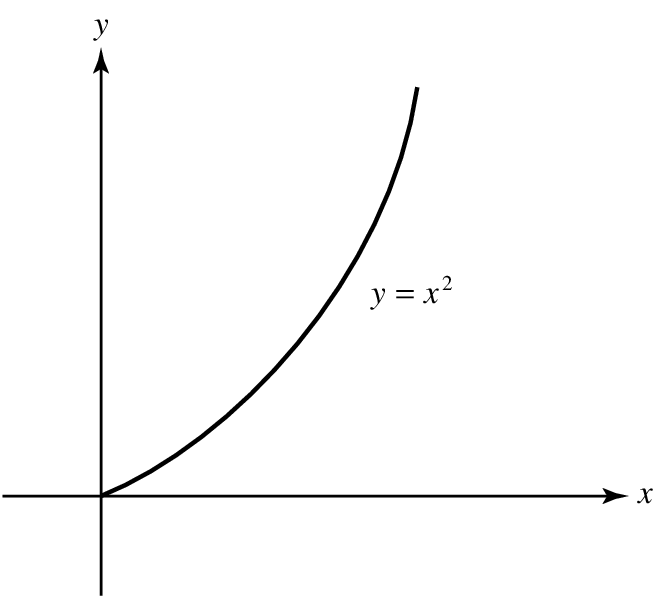
\includegraphics[width=2.3in,height=1.975in]{png/fig020105.png}
\end{center}
 \vskip6pt
 \refstepcounter{figure}
\nopagebreak
 \centerline{\bf Figure \thefigure} \label{figure:2.1.5}

\vskip2em
\noindent and
$h(x)=-x^3$
is decreasing on $(-\infty,\infty)$ (Figure~\ref{figure:2.1.6}).
\bbox\end{example}

 \vspace*{12pt}
\begin{center}
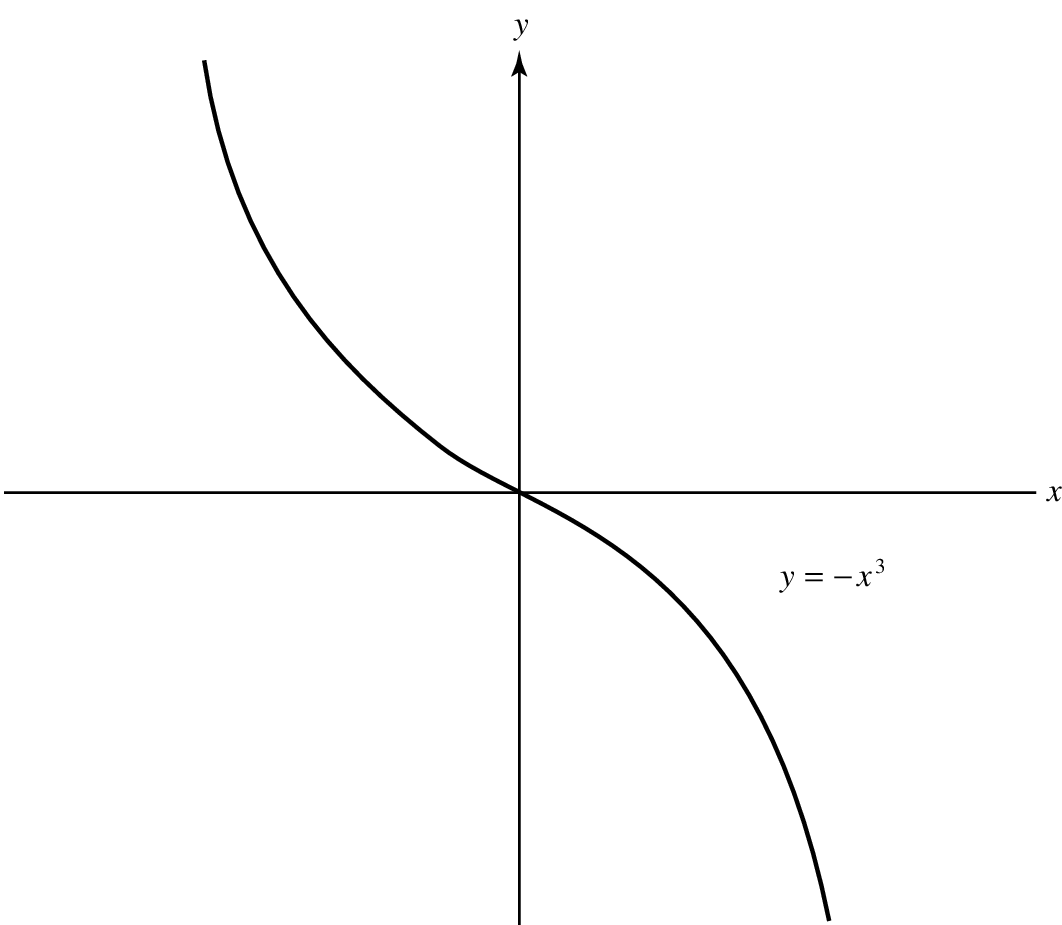
\includegraphics[width=3.6in,height=3.35in]{png/fig020106.png}
\end{center}
 \vskip6pt
 \refstepcounter{figure}
 \centerline{\bf Figure \thefigure} \label{figure:2.1.6}
 \vskip12pt

\newpage

In the proof of the following theorem, we assume that you have
formulated the definitions called for in Exercise~\ref{exer:2.1.19}.

\begin{theorem}\label{thmtype:2.1.9}
Suppose that $f$ is monotonic on $(a,b)$ and define
$$
\alpha=\inf_{a<x<b}f(x) \mbox{\quad and \quad}
\beta=\sup_{a<x<b}f(x).
$$

\begin{alist}
\item % (a)
 If $f$ is nondecreasing$,$ then
$f(a+)=\alpha$ and  $f(b-)=\beta.$
\item % (b)
If $f$ is nonincreasing$,$ then
$f(a+)=\beta$ and $f(b-)=\alpha.$ \\
$($Here $a+=-\infty$ if $a=-\infty$ and $b-=\infty$ if
$b=\infty.)$
\item %  (c)
 If $a<x_0<b$, then $f(x_0+)$ and $f(x_0-)$ exist and are
finite$\,;$ moreover$,$
$$
f(x_0-)\le f(x_0)\le f(x_0+)
$$
 if $f$ is
nondecreasing$,$ and
$$
f(x_0-)\ge f(x_0)\ge f(x_0+)
$$
 if $f$ is nonincreasing$.$
\end{alist}
\end{theorem}

\proof \part{a} We first show that $f(a+)=\alpha$. If

$M>\alpha$, there is an $x_0$ in $(a,b)$ such that $f(x_0)<M$. Since
$f$ is nondecreasing, $f(x)<M$ if $a<x<x_0$. Therefore, if
$\alpha=-\infty$, then $f(a+)=-\infty$. If $\alpha>-\infty$, let
$M=\alpha+\epsilon$, where $\epsilon>0$. Then $\alpha\le
f(x)<\alpha+\epsilon$, so
\begin{equation} \label{eq:2.1.20}
|f(x)-\alpha|<\epsilon\mbox{\quad if \quad} a<x<x_0.
\end{equation}
If $a=-\infty$,  this implies that $f(-\infty)=\alpha$. If
$a>-\infty$, let $\delta=x_0-a$. Then \eqref{eq:2.1.20} is equivalent to
$$
|f(x)-\alpha|<\epsilon\mbox{\quad if \quad} a<x<a+\delta,
$$
which implies that $f(a+)=\alpha$.

We now show that $f(b-)=\beta$. If $M<\beta$, there is an $x_0$ in
$(a,b)$ such that $f(x_0)>M$. Since $f$ is nondecreasing, $f(x)>M$ if
$x_0<x<b$. Therefore, if $\beta=\infty$, then $f(b-)=\infty$. If
$\beta<\infty$, let $M=\beta-\epsilon$, where $\epsilon>0$. Then
$\beta-\epsilon< f(x)\le\beta$, so
\begin{equation} \label{eq:2.1.21}
|f(x)-\beta|<\epsilon\mbox{\quad if \quad} x_0<x<b.
\end{equation}
If $b=\infty$,  this implies that $f(\infty)=\beta$. If $b<\infty$,
let $\delta=b-x_0$. Then \eqref{eq:2.1.21} is equivalent to
$$
|f(x)-\beta|<\epsilon\mbox{\quad if \quad} b-\delta<x<b,
$$
which implies that $f(b-)=\beta$.

\part{b} The proof is similar to the proof of
\part{a} (Exercise~\ref{exer:2.1.34}).

\part{c} Suppose that $f$ is nondecreasing. Applying \part{a} to $f$ on
$(a,x_0)$ and $(x_0,b)$ separately shows that
$$
f(x_0-)=\sup_{a<x<x_0}f(x)\mbox{\quad and \quad}
f(x_0+)=\inf_{x_0<x<b}f(x).
$$

\newpage
\noindent
However, if $x_1<x_0<x_2$, then
$$
f(x_1)\le f(x_0)\le f(x_2);
$$
 hence,
$$
f(x_0-)\le f(x_0)\le f(x_0+).
$$

We leave the case where $f$ is nonincreasing to you
(Exercise~\ref{exer:2.1.34}).
\bbox

\boxit{Limits Inferior and Superior}
We now introduce some concepts  related to limits. We leave the study
of these concepts mainly to the  exercises.

We say that $f$  is {\it bounded\/}  on a set
$S$ if there
is a constant $M<\infty$ such that $|f(x)|\le M$ for all $x$ in $S$.

\samepage{
\begin{definition} \label{thmtype:2.1.10}
Suppose that
 $f$  is bounded on $[a,x_0)$, where $x_0$ may be
finite or $\infty$. For
$a\le x<x_0$, define
\begin{eqnarray*}
S_f(x;x_0)\ar= \sup_{x\le t<x_0}f(t)\\\arraytext{and}\\
I_f(x;x_0)\ar= \inf_{x\le t<x_0}f(t).
\end{eqnarray*}
Then the
 {\it left limit superior of $f$ at
$x_0$} is defined to be
$$
\limsup_{x\to x_0-} f(x)=\lim_{x\to x_0-}S_f(x;x_0),
$$
and the
 {\it left limit inferior of $f$ at
$x_0$} is defined to be
$$
\liminf_{x\to x_0-}f(x)=\lim_{x\to x_0-}I_f(x;x_0).
$$
(If $x_0=\infty$,  we define $x_0-=\infty$.)
\end{definition}

\samepage{
\begin{theorem} \label{thmtype:2.1.11}
If $f$ is bounded on $[a,x_0),$
then $\beta=\limsup_{x\to x_0-}f(x)$ exists
and is the unique real number with the following properties$\,:$
\begin{alist}
\item % (a)
If $\epsilon>0$, there is an $a_1$ in $[a,x_0)$ such that
\begin{equation} \label{eq:2.1.22}
f(x)<\beta+\epsilon\mbox{\quad if \quad} a_1\le x<x_0.
\end{equation}
\item % (b)
If $\epsilon>0$ and $a_1$ is in $[a,x_0),$ then
$$
f(\overline x)>\beta-\epsilon\mbox{\quad for some }\overline
x\in[a_1,x_0).
$$
\end{alist}
\end{theorem}

\proof
Since $f$ is bounded on $[a,x_0)$, $S_f(x;x_0)$ is nonincreasing and
bounded on $[a,x_0)$. By applying Theorem~\ref{thmtype:2.1.9}\part{b} to
$S_f(x;x_0)$, we conclude that $\beta$
exists (finite). Therefore, if $\epsilon>0$, there is an $\overline a$
in
$[a,x_0)$ such that}

\begin{equation} \label{eq:2.1.23}
\beta-\epsilon/2<S_f(x;x_0)<\beta+\epsilon/2 \mbox{\quad if \quad}
\overline a\le x<x_0.
\end{equation}

\newpage
\noindent
Since $S_f(x;x_0)$ is an upper bound of $\set{f(t)}{x\le t<x_0}$,
$f(x)\le S_f(x;x_0)$.
Therefore, the second inequality in \eqref{eq:2.1.23} implies
\eqref{eq:2.1.22} with
$a_1=\overline a$. This proves \part{a}. To prove \part{b}, let $a_1$
be given and define $x_1=\max(a_1,\overline a)$. Then the first
inequality in
\eqref{eq:2.1.23} implies that}
\begin{equation} \label{eq:2.1.24}
S_f(x_1;x_0)>\beta-\epsilon/2.
\end{equation}
Since $S_f(x_1;x_0)$ is the supremum of $\set{f(t)}{x_1<t<x_0}$,
 there is an $\overline x$ in $[x_1,x_0)$ such that
$$
f(\overline x)>S_f(x_1;x_0)-\epsilon/2.
$$
This and \eqref{eq:2.1.24} imply that $f(\overline x)>\beta-\epsilon$.
Since $\overline x$ is in $[a_1,x_0)$, this proves \part{b}.

Now we show that there cannot be more than one real number with
properties \part{a} and \part{b}. Suppose that $\beta_1<\beta_2$ and
$\beta_2$ has property \part{b}; thus, if $\epsilon>0$ and $a_1$ is
in $[a,x_0)$, there is an
$\overline x$ in $[a_1,x_0)$ such that
$f(\overline x)>\beta_2-\epsilon$. Letting
$\epsilon=\beta_2-\beta_1$, we see that there is an $\overline x$ in
 $[a_1,b)$ such that
$$
f(\overline x)>\beta_2-(\beta_2-\beta_1)=\beta_1,
$$
so  $\beta_1$ cannot have property \part{a}. Therefore, there cannot
be more than one real number that satisfies both \part{a} and
\part{b}.
\bbox

The proof of the following theorem is similar to this
(Exercise~\ref{exer:2.1.35}).

\begin{theorem} \label{thmtype:2.1.12}
If $f$ is bounded on $[a,x_0),$
then $\alpha=\liminf_{x\to x_0-}f(x)$ exists
and is the unique real number with the following properties:

\begin{alist}
\item % (a)
If $\epsilon>0,$ there is an $a_1$ in $[a,x_0)$ such that
$$
f(x)>\alpha-\epsilon\mbox{\quad if \quad} a_1\le x<x_0.
$$
\item % (b)
If $\epsilon>0$ and $a_1$ is in $[a,x_0),$ then
$$
f(\overline x)<\alpha+\epsilon\mbox{\quad for some }\overline
x\in[a_1,x_0).
$$
\end{alist}
\end{theorem}

\exercises
\begin{exerciselist}

\item\label{exer:2.1.1}
Each of the following conditions fails to define a function on any
domain. State why.

\begin{tabular}[t]{@{}p{168pt}@{}p{168pt}}
 \part{a} $\sin f(x)=x$&\part{b} $e^{f(x)}=-|x|$\\\\
 \part{c} $1+x^2+[f(x)]^2=0$&
\part{d} $f(x)[f(x)-1]=x^2$
\end{tabular}

\item\label{exer:2.1.2}  If
$$
f(x)=\sqrt{\frac{(x-3)(x+2)}{ x-1}}
\mbox{\quad and \quad} g(x)=\frac{x^2-16}{ x-7}
\sqrt{x^2-9},
$$
find $D_f$, $D_{f\pm g}$, $D_{fg}$, and $D_{f/g}$.

\item\label{exer:2.1.3}  Find $D_f$.

\begin{tabular}[t]{@{}p{168pt}@{}p{168pt}}
 \part{a} $f(x)=\tan x$&\part{b} $f(x)=\dst\frac{1}{\sqrt{1-|\sin
x|}}$\\\\
 \part{c} $f(x)=\dst\frac{1}{ x(x-1)}$&\part{d}
$f(x)=\dst\frac{\sin x}{ x}$\\\\
 \part{e} $e^{[f(x)]^2}=x,\quad f(x)\ge0$\\\\
\end{tabular}

\item\label{exer:2.1.4}
Find $\lim_{x\to x_0}f(x)$, and justify your answers with an
$\epsilon$--$\delta$ proof.

\begin{tabular}[t]{@{}p{168pt}@{}p{168pt}}
 \part{a} $x^2+2x+1,\quad x_0=1$&\part{b} $\dst{\frac{x^3-8}{
x-2},\quad x_0=2}$\\
 \part{c} $\dst{\frac{1}{x^2-1},\quad x_0=0}$&\part{d}
$\sqrt{x},\quad x_0=4$\\[3\jot]
\part{e}
$\dst\frac{x^3-1}{(x-1)(x-2)}+x,\quad x_0=1$
\end{tabular}

\item\label{exer:2.1.5} Prove that
Definition~\ref{thmtype:2.1.2} is unchanged if Eqn.~\eqref{eq:2.1.4} is
replaced by
$$
|f(x)-L|<K\epsilon,
$$
where $K$ is any positive constant. (That is, $\lim_{x\to x_0} f(x)=L$
according to Definition~\ref{thmtype:2.1.2} if and only if $\lim_{x\to
x_0} f(x)=L$ according to the modified definition.)

\item\label{exer:2.1.6} Use
Theorem~\ref{thmtype:2.1.4} and the known limits $\lim_{x\to x_0} x=x_0$,
$\lim_{x\to x_0} c=c$ to find the indicated limits.

\begin{tabular}[t]{@{}p{168pt}@{}p{168pt}}
 \part{a} $\dst\lim_{x\to 2}\frac{x^2+2x+3}{2x^3+1}$&
\part{b} $\dst\lim_{x\to 2}\left(\frac{1}{x+1}-\frac{1}{
x-1}\right)$\\\\
\part{c} $\dst\lim_{x\to 1}\frac{x-1}{ x^3+x^2-2x}$&
\part{d} $\dst\lim_{x\to 1}\frac{x^8-1}{ x^4-1}$
\end{tabular}

\item\label{exer:2.1.7}
 Find $\lim_{x\to x_0-} f(x)$ and $\lim_{x\to
x_0+}f(x)$, if they exist.  Use $\epsilon$--$\delta$ proofs, where
applicable, to justify your answers.

\begin{tabular}{ll}%[t]{@{}p{168pt}@{}p{168pt}}
 \part{a} $\dst{\frac{x+|x|}{ x},\quad x_0=0}$&\part{b}
$\dst{x\cos \frac{1}{x}+\sin \frac{1}{x}+\sin \frac{1}{
|x|},\quad x_0
=0}$\\[2\jot]
 \part{c} $\dst{\frac{|x-1|}{x^2+x-2},\quad x_0=1}$&\part{d}
$\dst{\frac{x^2+x-2}{\sqrt{x+2}},\quad x_0=-2}$\\\\
\end{tabular}

\item\label{exer:2.1.8} Prove:
If $h(x)\ge0$ for $a<x<x_0$ and $\lim_{x\to x_0-}
h(x)$ exists, then
$\lim_{x\to x_0-} h(x)\\ \ge~0$.
Conclude from this that if $f_2(x)\ge f_1(x)$ for $a<x<x_0$,
then
$$
\lim_{x\to x_0-}f_2(x)\ge\lim_{x\to x_0-}f_1(x)
$$
if both limits exist.

\pagebreak

\item\label{exer:2.1.9}
\begin{alist}
\item % (a)
Prove: If $\lim_{x\to x_0} f(x)$ exists, there is a constant $M$
and a $\rho>0$ such that $|f(x)|\le M$ if $0<
|x-x_0|<\rho$. (We say then that $f$ is {\it bounded\/} on $\set{x}
{0<|x-x_0|<\rho}$.)
\item % (b)
 State similar results with ``$\lim_{x\to x_0}$'' replaced by
``$\lim_{x\to x_0-}$.''
\item % (b)
 State similar results with ``$\lim_{x\to x_0}$'' replaced by
``$\lim_{x\to x_0+}$.''
\end{alist}

\item\label{exer:2.1.10}
Suppose that $\lim_{x\to x_0} f(x)=L$ and $n$ is a positive integer.
Prove that $\lim_{x\to x_0}[f(x)]^n=L^n$ \part{a} by using
Theorem~\ref{thmtype:2.1.4} and induction; \part{b} directly from
Definition~\ref{thmtype:2.1.2}. \hint{You will find
Exercise~$\ref{exer:2.1.9}$ useful for $\part{b}.$}

\item\label{exer:2.1.11}
 Prove:  If $\lim_{x\to x_0} f(x)=L>0$, then $\lim_{x\to
x_0}\sqrt{f(x)}=\sqrt{L}$.

\item\label{exer:2.1.12} Prove
   Theorem~\ref{thmtype:2.1.6}.

\item\label{exer:2.1.13}
\begin{alist}
\item % (a)
Using the hint stated after Theorem~\ref{thmtype:2.1.6}, prove that
Theorem~\ref{thmtype:2.1.3} remains valid with ``$\lim_{x\to x_0}$''
replaced by ``$\lim_{x\to x_0-}$.''
\item % (b)
Repeat \part{a} for Theorem~\ref{thmtype:2.1.4}.
\end{alist}

\item\label{exer:2.1.14} Define the statement ``$\lim_{x\to-\infty}f(x)=L$.''

\item\label{exer:2.1.15}
Find $\lim_{x\to\infty}f(x)$ if it exists, and justify your
answer directly from
Definition~\ref{thmtype:2.1.7}.

\begin{tabular}[t]{@{}p{112pt}@{}p{112pt}@{}p{112pt}}
 \part{a} $\dst\frac{1}{x^2+1}$&\part{b} $\dst\frac{\sin
x}{|x|^\alpha}\quad (\alpha>0)$&\part{c} $\dst{\frac{\sin x}{
|x|^\alpha}\quad(\alpha\le0)}$\\ \\
 \part{d} $e^{-x}\sin x$&\part{e} $\tan x$&\part{f} $e^{-x^2}e^{2x}$
\end{tabular}

\item\label{exer:2.1.16}
Theorems~\ref{thmtype:2.1.3} and \ref{thmtype:2.1.4} remain valid with
``$\lim_{x\to x_0}$'' replaced throughout by ``$\lim_{x \to\infty}$''
(``$\lim_{x\to-\infty}$''). How would their proofs have to be changed?

\item\label{exer:2.1.17}
Using the definition you gave in Exercise~\ref{exer:2.1.14}, show that

\begin{tabular}[t]{@{}p{168pt}@{}p{168pt}}
 \part{a} $\dst\lim_{x\to-\infty}\left(1-\frac{1}{
x^2}\right)=1$&\part{b} $\dst\lim_{x\to-\infty} \frac{2|x|}{
1+x}=-2$\\\\
 \part{c} $\dst\lim_{x\to-\infty}\sin x$ does not
exist
\end{tabular}

\item\label{exer:2.1.18} Find $\lim_{x\to-\infty}f(x)$, if it exists, for
each function in Exercise~\ref{exer:2.1.15}. Justify your
answers directly from the definition you gave in
Exercise~\ref{exer:2.1.14}.

\item\label{exer:2.1.19} Define

\begin{tabular}[t]{@{}p{112pt}@{}p{112pt}@{}p{112pt}}
 \part{a} $\dst\lim_{x\to x_0-} f(x)=-\infty$& \part{b}
$\dst\lim_{x\to x_0+} f(x)=
\infty$&\part{c} $\dst\lim_{x\to x_0+} f(x)=-\infty$\\
\end{tabular}

\item\label{exer:2.1.20} Find

\begin{tabular}[t]{@{}p{168pt}@{}p{168pt}}
 \part{a} $\dst\lim_{x\to 0+}\frac{1}{ x^3}$&\part{b}
$\dst\lim_{x\to 0-}\frac{1}{ x^3}$\\\\
\end{tabular}

\begin{tabular}[t]{@{}p{168pt}@{}p{168pt}}
 \part{c} $\dst\lim_{x\to 0+}\frac{1}{ x^6}$&\part{d}
$\dst\lim_{x\to 0-}\frac{1}{ x^6}$\\\\
 \part{e} $\dst\lim_{x\to x_0+}\frac{1}{(x-x_0)^{2k}}$&\part{f}
$\dst\lim_{x\to x_0-}\frac{1}{(x-x_0)^{2k+1}}$\\
\hspace*{1.5em} ($k=$ positive integer)\\
\end{tabular}

\newpage

\item\label{exer:2.1.21} Define

\vspace*{3pt}

\begin{tabular}[t]{@{}p{168pt}@{}p{168pt}}
 \part{a} $\dst\lim_{x\to x_0}f(x)=\infty$&\part{b} $\dst\lim_{x\to x_0}
f(x)=-\infty$\\
\end{tabular}

\vspace*{3pt}

\item\label{exer:2.1.22} Find

\vspace*{3pt}

\begin{tabular}[t]{@{}p{168pt}@{}p{168pt}}
 \part{a} $\dst\lim_{x\to 0}\frac{1}{ x^3}$&\part{b}
$\dst\lim_{x\to 0}\frac{1}{ x^6}$\\\\
 \part{c} $\dst\lim_{x\to x_0}\frac{1}{(x-x_0)^{2k}}$&\part{d}
$\dst\lim_{x\to x_0}\frac{1}{(x-x_0)^{2k+1}}$\\
\hspace*{1.5em} ($k=$ positive integer)
\end{tabular}

\vspace*{3pt}

\item\label{exer:2.1.23} Define

\vspace*{3pt}

\begin{tabular}[t]{@{}p{168pt}@{}p{168pt}}
 \part{a} $\dst\lim_{x\to\infty} f(x)=\infty$&\part{b}
$\dst\lim_{x\to-\infty} f(x)=-\infty$
\end{tabular}

\vspace*{3pt}

\item\label{exer:2.1.24} Find

\vspace*{3pt}

\begin{tabular}[t]{@{}p{168pt}@{}p{168pt}}
 \part{a} $\dst\lim_{x\to\infty} x^{2k}$&\part{b} $\dst{\lim_{x\to-\infty}}
x^{2k}$\\\\
 \part{c} $\dst\lim_{x\to\infty} x^{2k+1}$&\part{d}
$\dst\lim_{x\to-\infty} x^{2k+1}$\\[2\jot]
 ($k$=positive integer)\\[2\jot]
 \part{e} $\dst\lim_{x\to\infty}\sqrt{x}\sin x$&
\part{f} $\dst\lim_{x\to\infty}e^x$
\end{tabular}

\vspace*{3pt}

\item\label{exer:2.1.25}
Suppose that $f$ and $g$ are defined   on $(a,\infty)$ and
$(c,\infty)$ respectively, and that $g(x)>a$ if $x>c$.
Suppose also that
$\lim_{x\to\infty}f(x)=L$, where $-\infty\le L\le \infty$, and
$\lim_{x\to\infty}g(x)=\infty$.
Show that $\lim_{x\to\infty}f(g(x))=L$.

\vspace*{3pt}

\item\label{exer:2.1.26}

\begin{alist}
\item % (a)
 Prove: $\lim_{x\to x_0}f(x)$ does not exist (finite) if
for some $\epsilon_0>0$,  every deleted neighborhood of $x_0$
contains points $x_1$ and $x_2$ such that
$$
|f(x_1)-f(x_2)|\ge\epsilon_0.
$$

\vspace*{3pt}

\item % (b)
Give analogous conditions for the nonexistence of
$$
\lim_{x\to
x_0+}f(x),\quad \lim_{x\to x_0-}f(x),\quad \lim_{x\to\infty}f(x),
\mbox{\quad and \quad}
 \lim_{x\to-\infty}f(x).
$$
\end{alist}

\vspace*{3pt}

\item\label{exer:2.1.27} Prove: If $-\infty<x_0<\infty$, then $\lim_{x\to
x_0}f(x)$ exists in the extended reals if and only if $\lim_{x\to
x_0-}f(x)$ and $\lim_{x\to x_0+}f(x)$ both exist in the extended
reals and are equal, in which case all three are equal.

\vspace*{3pt}

\exercisetext
 {In
Exercises~$\ref{exer:2.1.28}$--$\ref{exer:2.1.30}$
consider only the case where at least one of
$L_1$ and $L_2$ is $\pm\infty$.}

\vspace*{3pt}

\item\label{exer:2.1.28} Prove: If $\lim_{x\to x_0} f(x)=L_1$, $\lim_{x
\to x_0}g(x)=L_2$, and $L_1+L_2$ is not indeterminate, then
$$
\lim_{x\to x_0}(f+g)(x)=L_1+L_2.
$$

\newpage

\item\label{exer:2.1.29} Prove: If $\lim_{x\to\infty}f(x)=L_1$, $\lim_{x
\to\infty}g(x)=L_2$, and $L_1L_2$ is not indeterminate, then
$$
\lim_{x\to\infty}(fg)(x)=L_1L_2.
$$

\vspace*{3pt}

\item\label{exer:2.1.30}

\vspace*{3pt}

\begin{alist}
\item % (a)
 Prove:  If $\lim_{x\to x_0}f(x)=L_1$, $\lim_{x\to
x_0}g(x)=L_2\ne0$, and $L_1/L_2$ is not indeterminate, then
$$
\lim_{x\to x_0}\left(\frac{f}{ g}\right)(x)=\frac{L_1}{ L_2}.
$$

\vspace*{3pt}

\item % (b)
 Show that it is necessary to assume that $L_2\ne0$ in\part{a}
by considering $f(x)=\sin x$, $g(x)=\cos x$, and $x_0=\pi/2$.
\end{alist}

\vspace*{3pt}

\item\label{exer:2.1.31} Find

\vspace*{3pt}

\begin{tabular}[t]{@{}p{168pt}@{}p{168pt}}
 \part{a} $\dst\lim_{x\to 0+} \frac{x^3+2x+3}{
2x^4+3x^2+2}$&\part{b} $\dst\lim_{x\to 0-}\frac{x^3+2x+3}{
2x^4+3x^2+2}$\\\\
 \part{c} $\dst\lim_{x\to\infty}\frac{2x^4+3x^2+2}{
x^3+2x+3}$&\part{d}
$\dst\lim_{x\to -\infty}\frac{2x^4+3x^2+2}{ x^3+2x+3}$\\\\
 \part{e} $\lim_{x\to\infty}(e^{x^2}-e^x)$&\part{f}
$\dst\lim_{x\to\infty}\frac{x+\sqrt{x}\sin x}{2x+e^{-x}}$
\end{tabular}

\vspace*{3pt}

\item\label{exer:2.1.32} Find $\lim_{x\to\infty}r(x)$ and $\lim_{x
\to-\infty}r(x)$ for the rational function
$$
r(x)=\frac{a_0+a_1x+\cdots+a_nx^n}{ b_0+b_1x+\cdots+b_mx^m},
$$
where $a_n\ne0$ and $b_m\ne0$.

\vspace*{3pt}

\item\label{exer:2.1.33} Suppose that $\lim_{x\to x_0} f(x)$ exists for
every $x_0$ in $(a,b)$ and $g(x)=f(x)$ except on a set $S$ with no
limit points in $(a,b)$. What can be said about $\lim_{x\to x_0}
g(x)$ for $x_0$ in $(a,b)$? Justify your answer.

\vspace*{3pt}

\item\label{exer:2.1.34}
Prove Theorem~\ref{thmtype:2.1.9}\part{b}, and complete the proof
of Theorem~\ref{thmtype:2.1.9}\part{b} in the case where $f$ is
nonincreasing.
\vspace*{3pt}

\item\label{exer:2.1.35} Prove Theorem~\ref{thmtype:2.1.12}.

\vspace*{3pt}

\item\label{exer:2.1.36}

Show that if $f$ is bounded on $[a,x_0)$, then

\vspace*{3pt}

\begin{alist}
\item % (a)
 $\dst\liminf_{x\to x_0-} f(x)\le\dst\limsup_{x\to x_0-} f(x)$.

\vspace*{3pt}

\item % (b)
 $\dst\liminf_{x\to x_0-}(-f)(x)=-\dst\limsup_{x\to x_0-} f(x)$
and $\dst\limsup_{x\to x_0-}(-f)(x)=-\dst\liminf_{x\to x_0-} f(x)$.

\vspace*{3pt}

\item % (c)
 $\dst\liminf_{x\to x_0-} f(x)=\limsup_{x\to
x_0-} f(x)$ if and only if $\lim_{x\to x_0-}f(x)$ exists,
in which case
$$
\lim_{x\to x_0-} f(x)=\liminf_{x\to x_0-} f(x)=
\limsup_{x\to x_0-} f(x).
$$
\end{alist}

\vspace*{3pt}

\item\label{exer:2.1.37}
Suppose that $f$ and $g$ are bounded on $[a,x_0)$.

\newpage

\begin{alist}

\item % (a)
 Show that
$$
\limsup_{x\to x_0-} (f+g)(x)\le
\limsup_{x\to x_0-} f(x)+\limsup_{x\to x_0-} g(x).
$$
\item % (b)
Show that
$$
\liminf_{x\to x_0-} (f+g)(x)\ge
\liminf_{x\to x_0-} f(x)+\liminf_{x\to x_0-} g(x).
$$
\item % (c)
State inequalities analogous to those in  \part{a} and \part{b} for
$$
\liminf_{x\to x_0-} (f-g)(x)\mbox{\quad and \quad}\limsup_{x
\to x_0-}(f-g)(x).
$$
\end{alist}

\item\label{exer:2.1.38}
Prove: $\lim_{x\to x_0-} f(x)$ exists (finite)
if and only if for each $\epsilon>0$ there is a $\delta>0$ such that
$|f(x_1)-f(x_2)|<\epsilon$ if $x_0-\delta<x_1$, $x_2<x_0$.
\hint{For sufficiency$,$ show that $f$ is bounded on some interval
$(a,x_0)$ and
$$
\limsup_{x
\to0-}f(x)=\liminf_{x\to x_0-}f(x).
$$
 Then use
Exercise~$\ref{exer:2.1.36}\part{c}.$}

\item\label{exer:2.1.39}
Suppose that $f$ is bounded on an interval $(x_0,b]$. Using
Definition~\ref{thmtype:2.1.10} as a guide, define $\limsup_{x\to
x_0+}f(x)$
({\it the right limit superior of $f$ at $x_0$}) and $\liminf_{x\to
x_0+}f(x)$ ({\it the right limit inferior of $f$ at $x_0$}). Then
prove that they exist. \hint{Use Theorem~$\ref{thmtype:2.1.9}.$}

\item\label{exer:2.1.40}
Suppose that $f$ is bounded on an interval $(x_0,b]$. Show that
 $\liminf_{x\to x_0+} f(x)=\limsup_{x\to
x_0+} f(x)$ if and only if $\lim_{x\to x_0+}f(x)$ exists,
in which case
$$
\lim_{x\to x_0+} f(x)=\liminf_{x\to x_0+} f(x)=
\limsup_{x\to x_0+} f(x).
$$

\item\label{exer:2.1.41}
Suppose that $f$ is bounded on an open interval containing $x_0$. Show that
$\lim_{x\to x_0}f(x)$ exists if and only if
$$
\limsup_{x\to x_0-} f(x)=\limsup_{x\to x_0+} f(x)=
\liminf_{x\to x_0-}f(x)=\liminf_{x\to x_0+}f(x),
$$
in which case $\lim_{x\to x_0}f(x)$ is the common value of these four
expressions.
\label{sectionend:\thesection}

\end{exerciselist}

\currentpdfbookmark{Section 2.2 Continuity}{section:2.2}
\newsection{2}{Differential Calculus of Functions of One Variable
}{Continuity}


\renewcommand{\thissection}{\sectiontitle{CONTINUITY}}
\thissection


\noindent
In this section we study continuous functions of a real variable. We
will prove some important theorems about continuous functions that,
although intuitively plausible, are beyond the scope of the elementary
calculus course. They are accessible now because of our better
understanding of the real number system, especially of those
properties that stem from the completeness axiom.

\newpage
The definitions of
$$
f(x_0-)=\lim_{x\to x_0-}f(x),\quad f(x_0+)=\lim_{x\to
x_0+}f(x),\mbox{\quad and \quad}
\lim_{x\to x_0} f(x)
$$
do not involve $f(x_0)$ or even require that it be defined. However,
the case where $f(x_0)$ is defined and equal to one or more of these
quantities is important.

\begin{definition}\label{thmtype:2.2.1}
\vspace{6pt}
\begin{alist}
\item % (a)
We say that $f$ is {\it continuous at $x_0$\/} if $f$ is
defined on an open interval $(a,b)$ containing $x_0$ and $\lim_{x\to
x_0}f(x)=f(x_0)$.
\item % (b)
We say that $f$ is {\it continuous from the left at $x_0$\/} if $f$ is
defined on an open interval $(a,x_0)$ and $f(x_0-)=f(x_0)$.
\item % (c)
We say that $f$ is {\it continuous from the right at $x_0$\/} if $f$
is defined on an open interval $(x_0,b)$ and $f(x_0+)=f(x_0)$.
\bbox
\end{alist}
\end{definition}

The following theorem provides a method for determining whether these
definitions are satisfied.  The proof, which we leave to you
(Exercise~\ref{exer:2.2.1}), rests on
Definitions~\ref{thmtype:2.1.2}, \ref{thmtype:2.1.5},
and \ref{thmtype:2.2.1}.

\enlargethispage{\baselineskip}

\begin{theorem}\label{thmtype:2.2.2}\mbox{}
\vspace*{6pt}
\begin{alist}
\item % (a)
A function $f$ is continuous at $x_0$ if and only if $f$ is defined on
an open interval $(a,b)$ containing $x_0$ and for each
$\epsilon>0$ there is a $\delta >0$ such that
\begin{equation}\label{eq:2.2.1}
|f(x)-f(x_0)|<\epsilon
\end{equation}
whenever $|x-x_0|<\delta.$
\item % (b)
A function $f$ is continuous from the right at $x_0$ if and only if
$f$ is defined on an interval $[x_0,b)$ and for each $\epsilon>
0$
there is a $\delta>0$ such that $\eqref{eq:2.2.1}$ holds whenever $x_0\le
x<x_0+ \delta.$
\item % (c)
A function $f$ is continuous from the left at $x_0$ if and only if $f$
is defined on an interval $(a,x_0]$ and for each $\epsilon >0$

there is a $\delta>0$ such that $\eqref{eq:2.2.1}$ holds whenever
$x_0-\delta<x\le x_0.$
\end{alist}
\end{theorem}

From Definition~\ref{thmtype:2.2.1} and Theorem~\ref{thmtype:2.2.2}, $f$ is

continuous at $x_0$ if and only if
$$
f(x_0-)=f(x_0+)=f(x_0)
$$
or, equivalently, if and only if it is continuous from the right and
left at $x_0$ (Exercise~\ref{exer:2.2.2}).

\begin{example}\label{example:2.2.1}\rm  Let $f$ be defined on $[0,2]$ by
$$
f(x)=\left\{\casespace\begin{array}{ll} x^2,&0\le x<1,\\
x+1,&1\le x\le2\end{array}\right.
$$

\newpage

\noindent (Figure~\ref{figure:2.2.1}); then
\begin{eqnarray*}
f(0+)\ar=0=f(0),\\
f(1-)\ar=1\ne f(1)=2,\\
f(1+)\ar=2=f(1),\\
f(2-)\ar=3=f(2).
\end{eqnarray*}
Therefore, $f$ is continuous from the right at $0$ and $1$ and
continuous
from the left at $2$, but not at $1$.  If $0<x$, $x_0<1$, then
\begin{eqnarray*}
|f(x)-f(x_0)|\ar =|x^2-x^2_0|=|x-x_0|\,|x+x_0|\\
\ar\le 2|x-x_0|<\epsilon\mbox{\quad if \quad}\ |x-x_0|<\epsilon/2.
\end{eqnarray*}
Hence, $f$ is continuous at each $x_0$ in $(0,1)$.  If $1<x$, $x_0<2$,
then
\begin{eqnarray*}
|f(x)-f(x_0)|\ar =|(x+1)-(x_0+1)=|x-x_0|\\
\ar<\epsilon\mbox{\quad if \quad}\ |x-x_0|<\epsilon.
\end{eqnarray*}
Hence, $f$ is continous at each $x_0$ in $(1, 2)$.
\end{example}

 \vspace*{12pt}
\begin{center}
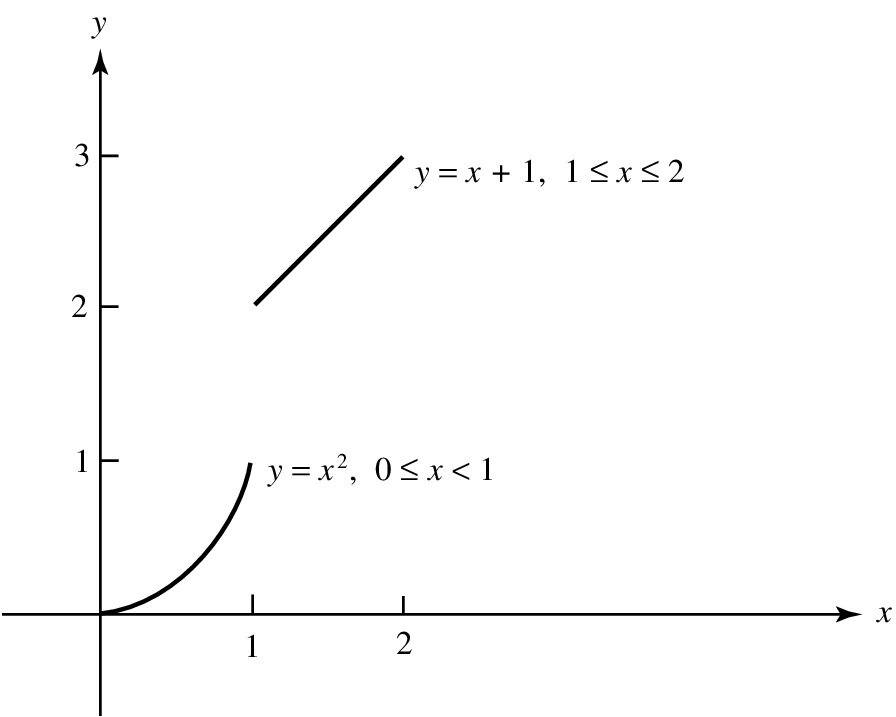
\includegraphics[width=3.05in,height=2.425in]{png/fig020201.png}
\end{center}
 \vskip6pt
 \refstepcounter{figure}
 \centerline{\bf Figure \thefigure} \label{figure:2.2.1}
 \vskip12pt

\begin{definition}\label{thmtype:2.2.3}
A function $f$ is {\it continuous on an open interval\/} $(a,b)$ if it
is continuous at every point in $(a,b)$. If, in addition,
\begin{eqnarray}
f(b-)=f(b)\label{eq:2.2.2}\\ \arraytext{or}\nonumber\\
f(a+)=f(a)\label{eq:2.2.3}
\end{eqnarray}

\newpage
\noindent
 then $f$ is {\it
continuous on $(a,b]$ or $[a,b)$\/}, respectively. If $f$ is
continuous on $(a,b)$ and \eqref{eq:2.2.2} and \eqref{eq:2.2.3} both hold,
then {\it $f$ is continuous on $[a,b]$\/}. More generally, if $S$ is a
subset of $D_f$ consisting of finitely or infinitely many disjoint
intervals, then $f$ is {\it continuous on $S$\/} if $f$ is continuous
on every interval in $S$. (Henceforth, in
connection with functions of one variable, whenever we say ``$f$
is continuous on $S$'' we mean that $S$ is a set of this kind.)
\end{definition}

\begin{example}\label{example:2.2.2}\rm   Let $f(x)=\sqrt{x}$, $0\le
x<\infty$. Then
$$
|f(x)-f(0)|=\sqrt{x}<\epsilon\mbox{\quad if \quad} 0\le
x<\epsilon^2,
$$
so $f(0+)=f(0)$.
If $x_0>0$ and $x\ge0$, then
\begin{eqnarray*}
|f(x)-f(x_0)|\ar =|\sqrt{x}-\sqrt{x_0}|=\frac{|x-x_0|}{\sqrt{x}+
\sqrt{x_0}}\nonumber\\
\ar\le  \frac{|x-x_0|}{\sqrt{x_0}}<\epsilon\mbox{\quad if \quad} |x-x_0|<
\epsilon\sqrt{x_0},
\end{eqnarray*}
so $\lim_{x\to x_0} f(x)=f(x_0)$. Hence, $f$ is continuous on
$[0,\infty)$.
\end{example}

\begin{example}\label{example:2.2.3}\rm    The function
$$
g(x)=\frac{1}{\sin\pi x}
$$
is continuous on  $S=\bigcup^\infty_{n=-\infty} (n,n+1)$.
However, $g$ is not continuous at any  $x_0=n$ (integer), since
it is not defined at such points.
\bbox\end{example}

The function $f$  defined in Example~\ref{example:2.2.1} (see also
Figure~\ref{figure:2.2.1}) is continuous on $[0,1)$ and $[1,2]$, but not
on any open interval containing 1. The discontinuity of $f$ there is
of the simplest kind, described in the following definition.

\enlargethispage{10pt}
\begin{definition}\label{thmtype:2.2.4}
 A function $f$ is
{\it piecewise continuous\/} on $[a,b]$ if

\begin{alist}
\item % (a)
 $f(x_0+)$ exists for all $x_0$ in $[a,b)$;
\item % (b)
 $f(x_0-)$ exists for all $x_0$ in $(a,b]$;
\item % (c)
 $f(x_0+)=f(x_0-)=f(x_0)$ for all but finitely many points
$x_0$ in $(a,b)$.
\end{alist}
If \part{c} fails to hold at some $x_0$ in $(a,b)$, $f$
has a {\it jump discontinuity at $x_0$\/}. Also, $f$ has
a {\it jump discontinuity at $a$\/} if $f(a+)\ne f(a)$ or {\it at\/}
$b$ if $f(b-)\ne f(b)$.
\end{definition}

\begin{example}\label{example:2.2.4}\rm   The function
$$
f(x)=\left\{\casespace\begin{array}{rl}1,&x=0,\\
 x,&0<x<1,\\
 2,&x=1,\\
 x,&1<x\le2,\\
-1,&2<x<3,\\
 0,&x=3,\end{array}\right.
$$
(Figure~\ref{figure:2.2.2}) is the graph of a piecewise continuous
function on $[0,3]$, with jump discontinuities at $x_0=0$, $1$, $2$,
and $3$.
\end{example}

\topfig{-3}
\begin{center}
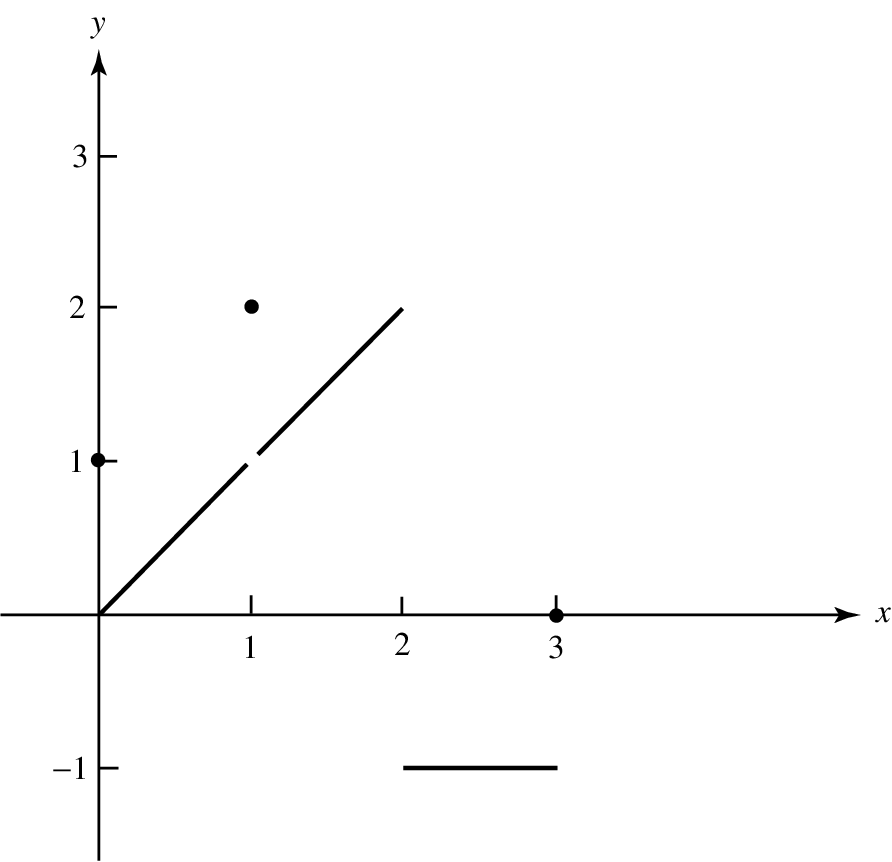
\includegraphics[width=3in,height=2.9in]{png/fig020202.png}
\end{center}
 \vskip6pt
 \refstepcounter{figure}
 \centerline{\bf Figure \thefigure} \label{figure:2.2.2}
 \vskip12pt

The reason for the adjective ``jump'' can be seen
in Figures~\ref{figure:2.2.1}
and \ref{figure:2.2.2}, where the graphs exhibit
a definite jump at each point of discontinuity. The next example
shows that not
all discontinuities are of this kind.

\begin{example}\label{example:2.2.5}\rm   The function
$$
f(x)=\left\{\casespace\begin{array}{ll}\sin\dst{\frac{1}{x}},&x\ne0,\\\\
 0,&x=0,\end{array}\right.
$$
is continuous at all $x_0$ except $x_0=0$. As $x$ approaches $0$ from
either side, $f(x)$ oscillates between $-1$ and $1$ with
ever-increasing frequency,  so neither $f(0+)$ nor $f(0-)$ exists.
Therefore, the discontinuity of $f$ at $0$ is not a jump
discontinuity, and if $\rho>0$, then $f$ is not piecewise continuous
on any interval
of the form $[-\rho,0]$, $[-\rho,\rho]$, or $[0,\rho]$.
\bbox\end{example}

Theorems~\ref{thmtype:2.1.4} and \ref{thmtype:2.2.2}
imply the next theorem
(Exercise~\ref{exer:2.2.18}).


\begin{theorem}\label{thmtype:2.2.5}
If $f$ and $g$ are continuous on a
set $S,$ then so are $f+g,$ $f-g,$ and $fg.$ In addition$,$ $f/g$ is
continuous at each $x_0$ in $S$ such that $g(x_0)\ne0.$
\end{theorem}

\begin{example}\label{example:2.2.6}\rm Since the constant functions and the
function $f(x)=x$ are continuous for all $x$, successive applications
of the various parts of Theorem~\ref{thmtype:2.2.5} imply that the
function
$$
r(x)=\frac{9-x^2}{ x+1}
$$

\newpage
\noindent
is continuous for all $x$ except $x=-1$ (see
Example~\ref{example:2.1.7}).
More generally, by starting from Theorem~\ref{thmtype:2.2.5} and using

induction, it can be shown that if $f_1$, $f_2$, \dots, $f_n$ are
continuous
on a set $S$, then so are $f_1+f_2+\cdots+f_n$ and $f_1f_2\cdots
f_n$. Therefore, any rational function
$$
r(x)=\frac{a_0+a_1x+\cdots+a_nx^n}{ b_0+b_1x+\cdots+b_mx^m}\quad
(b_m\ne0)
$$
is continuous for all values of $x$ except those for which its
denominator vanishes.\mbox{}
\end{example}

\boxit{Removable Discontinuities}
Let $f$ be defined on a deleted neighborhood of $x_0$ and
discontinuous (perhaps even undefined) at $x_0$. We say that $f$ has a
 at $x_0$ if $\lim_{x\to x_0}f(x)$ exists. In this case, the function
$$
g(x)=\left\{\casespace\begin{array}{ll} f(x)&\mbox{ if }
x\in D_f\mbox{ and } x\ne x_0,\\[2\jot]
\dst{\lim_{x\to x_0}} f(x)&\mbox{ if }
x=x_0,\end{array}\right.
$$
is continuous at $x_0$.

\begin{example}\label{example:2.2.7}\rm   The function
$$
f(x)=x\sin \frac{1}{ x}
$$
is not defined at $x_0=0$, and therefore certainly  not continuous
there, but $\lim_{x\to 0}f(x)=0$
(Example~\ref{example:2.1.6}).
Therefore, $f$ has a removable discontinuity at $0$.

The function
$$
f_1(x)=\sin\frac{1}{ x}
$$
is  undefined at $0$ and its discontinuity there is not
removable, since $\lim_{x\to 0} f_1(x)$ does not exist
(Example~\ref{example:2.2.5}).
\end{example}

\boxit{Composite Functions}
We have seen that the investigation of limits and continuity can be
simplified by regarding a given function as the result of addition,
subtraction, multiplication, and division of simpler functions.
Another operation useful in this connection is {\it composition\/} of
functions; that is, substitution of one
function into another.

 \begin{definition}\label{thmtype:2.2.6}
Suppose that $f$ and $g$ are functions with domains $D_f$ and $D_g$.
If $D_g$ has a nonempty subset
$T$ such that  $g(x)\in D_f$ whenever $x\in T$, then the
{\it composite function\/} $f\circ g$ is defined on $T$ by
$$
(f\circ g)(x)=f(g(x)).
$$
\end{definition}

\begin{example}\label{example:2.2.8}\rm   If
$$
f(x)=\log x\mbox{\quad and \quad} g(x)=\frac{1}{1-x^2},
$$
then
$$
D_f=(0,\infty)\mbox{\quad and \quad} D_g=\set{x}{x\ne\pm 1}.
$$
Since $g(x)>0$ if $x\in T=(-1,1)$, the composite function $f\circ g$
is defined on $(-1,1)$ by
$$
(f\circ g)(x)=\log \frac{1}{1-x^2}.
$$
 We leave it to you to verify that  $g\circ f$
is defined on $(0,1/e)\cup (1/e,e)\cup (e,\infty)$ by
$$
(g\circ f)(x)=\frac{1}{1-(\log x)^2}.
\eqno{\bbox}
$$
\end{example}

The next theorem says that the composition of  continuous functions
 is continuous.


\begin{theorem}\label{thmtype:2.2.7}
Suppose that $g$ is continuous at $x_0,$ $g(x_0)$ is an interior point
of $D_f,$ and $f$ is continuous at $g(x_0).$ Then
 $f\circ g$ is continuous at $x_0.$
\end{theorem}

\proof
 Suppose that $\epsilon>0$.  Since $g(x_0)$ is an interior
point of $D_f$ and  $f$ is continuous at $g(x_0)$, there is a
$\delta_1>0$ such that $f(t)$ is defined and
\begin{equation}\label{eq:2.2.4}
|f(t)-f(g(x_0))|<\epsilon\mbox{\quad if \quad} |t-g(x_0)|<
\delta_1.
\end{equation}
Since $g$ is continuous at $x_0$, there is a $\delta>0$ such that
$g(x)$ is defined and
\begin{equation}\label{eq:2.2.5}
|g(x)-g(x_0)|<\delta_1\mbox{\quad if \quad}|x-x_0|<\delta.
\end{equation}
Now \eqref{eq:2.2.4} and \eqref{eq:2.2.5} imply that
$$
|f(g(x))-f(g(x_0))|<\epsilon\mbox{\quad if \quad}|x-x_0|<\delta.
$$
 Therefore, $f\circ g$ is continuous at $x_0$.
\bbox

See Exercise~\ref{exer:2.2.22} for a related result concerning limits.

\begin{example}\label{example:2.2.9}\rm In Examples~\ref{example:2.2.2} and
\ref{example:2.2.6} we saw that the function
$$
f(x)=\sqrt{x}
$$
is continuous for $x>0$, and the function
$$
g(x)=\frac{9-x^2}{ x+1}
$$
is continuous for $x\ne-1$.  Since $g(x)>0$ if $x<-3$ or $-1<x<
3$,
Theorem~\ref{thmtype:2.2.7} implies that the function
$$
(f\circ g)(x)=\sqrt{\frac{9-x^2}{ x+1}}
$$
is continuous on $(-\infty,-3)\cup (-1,3)$.  It is also continuous from
the left at $-3$ and~$3$.
\end{example}

\newpage

\boxit{Bounded Functions}
A function $f$ is {\it bounded below\/}
on a set
$S$ if there is a real number $m$ such that
$$
f(x)\ge m \mbox{ for all } x\in S.
$$
In this case, the set
$$
V=\set{f(x)}{x\in S}
$$
has an infimum $\alpha$, and we write
$$
\alpha=\inf_{x\in S}f(x).
$$
If there is a point $x_1$ in $S$ such that
$f(x_1)=\alpha$,  we say that $\alpha$ is the {\it
minimum of $f$ on $S$}, and write
$$
\alpha=\min_{x\in S}f(x).
$$
Similarly, $f$ is {\it bounded above on $S$\/}
 if there is a real number
$M$ such that $f(x)\le M$ for all $x$ in $S$. In this case, $V$ has a
supremum $\beta$, and we write
$$
\beta=\sup_{x\in S}f(x).
$$
If there is a point $x_2$ in $S$ such that
$f(x_2)=\beta$,  we  say that $\beta$ is the {\it
maximum of $f$ on $S$}, and write
$$
\beta=\max_{x\in S}f(x).
$$
If $f$ is bounded above and below on a set $S$, we say that $f$ is
{\it bounded\/} on $S$.

Figure~\ref{figure:2.2.3} illustrates the geometric meaning of these
definitions for a function $f$ bounded on an interval $S=[a,b]$. The
graph of $f$ lies in the strip bounded by the lines $y=M$ and
$y=m$, where $M$ is any upper bound and $m$ is any lower bound
for $f$ on $[a,b]$. The narrowest strip containing the graph is the
one bounded above by $y=\beta= \sup_{a\le x\le b}f(x)$
and below by
$y=\alpha=\inf_{a\le x\le b}f(x)$.

 \vspace*{12pt}

\begin{center}
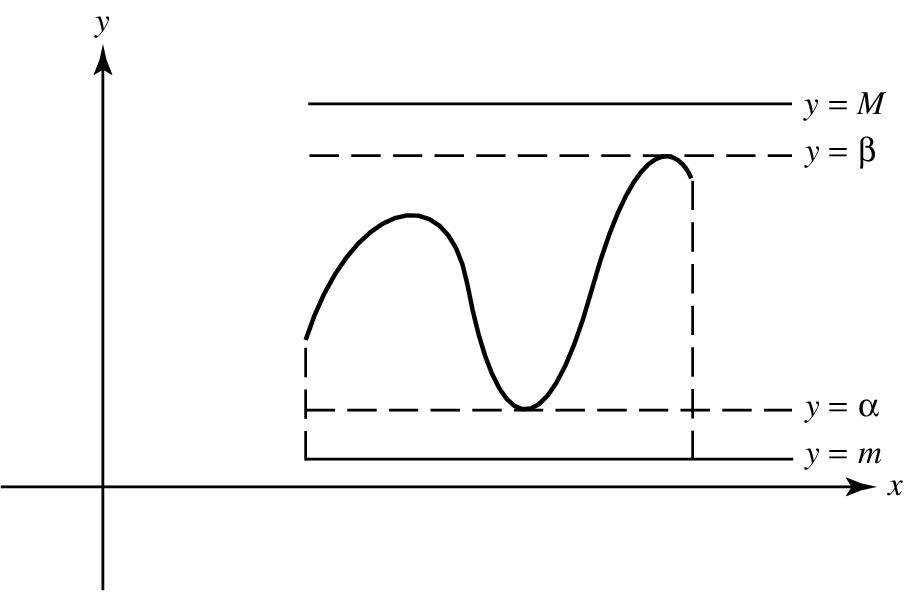
\includegraphics[width=3.1in,height=2.0in]{png/fig020203.png}
\end{center}
 \vskip6pt
 \refstepcounter{figure}
 \centerline{\bf Figure \thefigure} \label{figure:2.2.3}
 \vskip12pt

\begin{example}\label{example:2.2.10}\rm    The function
$$
g(x)=\left\{\casespace\begin{array}{ll}\frac{1}{2},&x=0
 \mbox{\quad or \quad}  x=1,\\[2\jot]
1-x,&0<x<1,\end{array}\right.
+$$
(Figure~\ref{figure:2.2.4}\part{a}) is bounded on $[0,1]$,
and
$$
\sup_{0\le x\le1}g(x)=1,\quad
\inf_{0\le x\le1}g(x)=0.
$$
 Therefore, $g$ has no maximum or minimum on $[0,1]$, since it does
not assume either of the values $0$ and $1$.

The function
$$
h(x)=1-x,\quad 0\le x\le1,
$$
which differs from $g$ only at $0$ and $1$
(Figure~\ref{figure:2.2.4}\part{b}), has the same supremum and
infimum as $g$, but it attains these values at $x=0$ and
$x=1$, respectively; therefore,
$$
\max_{0\le x\le1}h(x)=1\mbox{\quad and\quad}
\min_{0\le x\le1}h(x)=0.
$$
\end{example}

 \vspace*{12pt}
\begin{center}
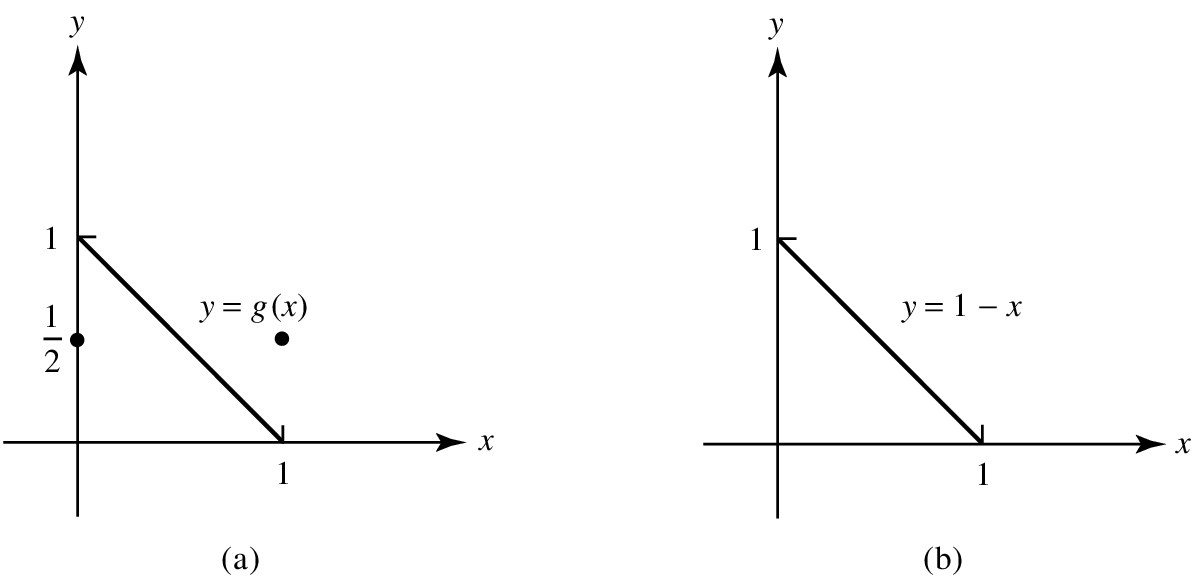
\includegraphics[width=4in,height=2in]{png/fig020204.png}
\end{center}
 \vskip6pt
 \refstepcounter{figure}
 \centerline{\bf Figure \thefigure} \label{figure:2.2.4}
 \vskip12pt

\begin{example}\label{example:2.2.11}\rm   The function
$$
f(x)=e^{x(x-1)}\sin \frac{1}{x(x-1)},\quad 0<x<1,
$$
oscillates between $\pm e^{x(x-1)}$ infinitely often in every interval
of the form $(0,\rho)$ or $(1-\rho,1)$, where $0<\rho<1$, and
$$
\sup_{0< x<1}f(x)=1,\quad\inf_{0<x<1}f(x)=-1.
$$
However, $f$ does not assume these values, so $f$ has no
maximum or minimum on $(0,1)$.
\end{example}

\begin{theorem}\label{thmtype:2.2.8}
If $f$ is continuous on a finite closed interval $[a,b],$ then $f$ is
bounded on $[a,b].$
\end{theorem}

\proof
 Suppose that $t\in [a,b]$. Since $f$ is continuous at $t$,
there is an open interval $I_t$ containing $t$ such
that
\begin{equation}\label{eq:2.2.7}
|f(x)-f(t)|<1 \mbox{\quad if \quad}\ x\in I_t\cap [a,b].
\end{equation}
(To see this, set $\epsilon=1$ in \eqref{eq:2.2.1},
Theorem~\ref{thmtype:2.2.2}.) The collection
${\mathcal H}=\set{I_t}{a\le t\le b}$
is an open covering of $[a,b]$. Since $[a,b]$ is compact, the
Heine--Borel theorem implies that there are finitely many points
$t_1$,
$t_2$, \dots, $t_n$ such that the intervals $I_{t_1}$,
$I_{t_2}$, \dots, $I_{t_n}$
cover $[a,b]$. According to \eqref{eq:2.2.7} with $t=t_i$,
$$
|f(x)-f(t_i)|<1\mbox{\quad if \quad}\ x\in I_{t_i}\cap [a,b].
$$
Therefore,
\begin{equation}\label{eq:2.2.8}
\begin{array}{rcl}
|f(x)|\ar =|(f(x)-f(t_i))+f(t_i)|\le|f(x)-f(t_i)|+|f(t_i)|\\[2\jot]
\ar\le  1+|f(t_i)|\mbox{\quad if \quad}\
x\in I_{t_i}\cap[a,b].
\end{array}
\end{equation}
 Let
$$
M=1+\max_{1\le i\le n}|f(t_i)|.
$$
Since $[a,b]\subset\bigcup^n_{i=1}\left(I_{t_i}\cap
[a,b]\right)$, \eqref{eq:2.2.8} implies that
$|f(x)|\le M$ if  $x\in [a,b]$.
\bbox


This proof illustrates the utility of the Heine--Borel theorem, which
allows us to choose $M$ as the largest of a {\it finite\/} set of
numbers.

Theorem~\ref{thmtype:2.2.8} and the completeness of the reals imply that


if $f$ is continuous on a finite closed interval $[a,b]$, then $f$ has
an infimum and a supremum on $[a,b]$.
The next theorem shows that $f$ actually assumes these values
at some points in $[a,b]$.


\begin{theorem}\label{thmtype:2.2.9}
Suppose that $f$ is continuous on a finite closed interval $[a,b].$ Let
$$
\alpha=\inf_{a\le x\le b}f(x)\mbox{\quad and
\quad}\beta=\sup_{a\le x\le b}f(x).
$$
Then $\alpha$ and $\beta$ are respectively the minimum
and maximum of $f$ on $[a,b];$ that is$,$
 there are points $x_1$ and $x_2$ in $[a,b]$ such that
$$
f(x_1)=\alpha\mbox{\quad and \quad} f(x_2)=\beta.
$$
\end{theorem}

\proof
We show that $x_1$ exists and leave it to you to show that $x_2$
exists (Exercise~\ref{exer:2.2.24}).

Suppose that there is no
$x_1$ in $[a,b]$ such that $f(x_1)=\alpha$. Then $f(x)>\alpha$
for all $x\in[a,b]$. We will show that this leads to a
contradiction.

Suppose that $t\in[a,b]$.
Then $f(t)>\alpha$, so
$$
f(t)>\frac{f(t)+\alpha}{2}>\alpha.
$$

\enlargethispage{1in}
\newpage
\noindent
Since $f$ is continuous at $t$, there is an open interval $I_t$ about
$t$ such that
\begin{equation}\label{eq:2.2.9}
f(x)>\frac{f(t)+\alpha}{2}\mbox{\quad if \quad} x\in
I_t\cap [a,b]
\end{equation}
(Exercise~\ref{exer:2.2.15}). The collection ${\mathcal H}=\set{I_t}{a\le t\le
b}$ is an open covering of $[a,b]$. Since $[a,b]$ is compact, the
Heine--Borel theorem implies that there are finitely many points $t_1$,
$t_2$, \dots, $t_n$ such that the intervals $I_{t_1}$,
$I_{t_2}$, \dots,
$I_{t_n}$ cover $[a,b]$. Define
$$
\alpha_1=\min_{1\le i\le n}\frac{f(t_i)+\alpha}{2}.
$$
Then, since $[a,b]\subset\bigcup^n_{i=1} (I_{t_i}\cap [a,b])$,
\eqref{eq:2.2.9} implies that
$$
f(t)>\alpha_1,\quad a\le t\le b.
$$
But $\alpha_1>\alpha$, so this contradicts the definition of $\alpha$.
Therefore, $f(x_1)=\alpha$ for some $x_1$ in $[a,b]$.
\bbox

\begin{example}\label{example:2.2.12}\rm We used the compactness of
$[a,b]$ in the proof of Theorem~\ref{thmtype:2.2.9} when
we invoked the Heine--Borel theorem. To see that compactness
is essential to the proof, consider the function
$$
g(x)=1-(1-x)\sin\frac{1}{ x},
$$
which is continuous and has supremum  $2$ on the
noncompact interval $(0,1]$, but does not assume its supremum on
$(0,1]$, since
\begin{eqnarray*}
g(x)\ar\le 1+(1-x)\left|\sin\frac{1}{ x}\right|\\
\ar\le 1+(1-x)<2 \mbox{\quad if \quad} 0<x\le1.
\end{eqnarray*}
As another example, consider the function
$$
f(x)=e^{-x},
$$
which is continuous and has infimum $0$, which it does
not attain, on the noncompact interval $(0,\infty)$.
\bbox\end{example}

The next theorem shows that if $f$ is continuous on a finite closed
interval
$[a,b]$, then $f$ assumes every value between $f(a)$ and $f(b)$ as $x$
varies from $a$ to $b$ (Figure~\ref{figure:2.2.5},
page~\pageref{figure:2.2.5}).


\begin{theorem}[Intermediate Value Theorem] \label{thmtype:2.2.10}
Suppose that $f$ is continuous on $[a,b],$ $f(a)\ne f(b),$ and $\mu$
is between $f(a)$ and $f(b).$ Then $f(c)=\mu$ for some
$c$ in $(a,b).$
\end{theorem}

\topfig{-3}
\begin{center}
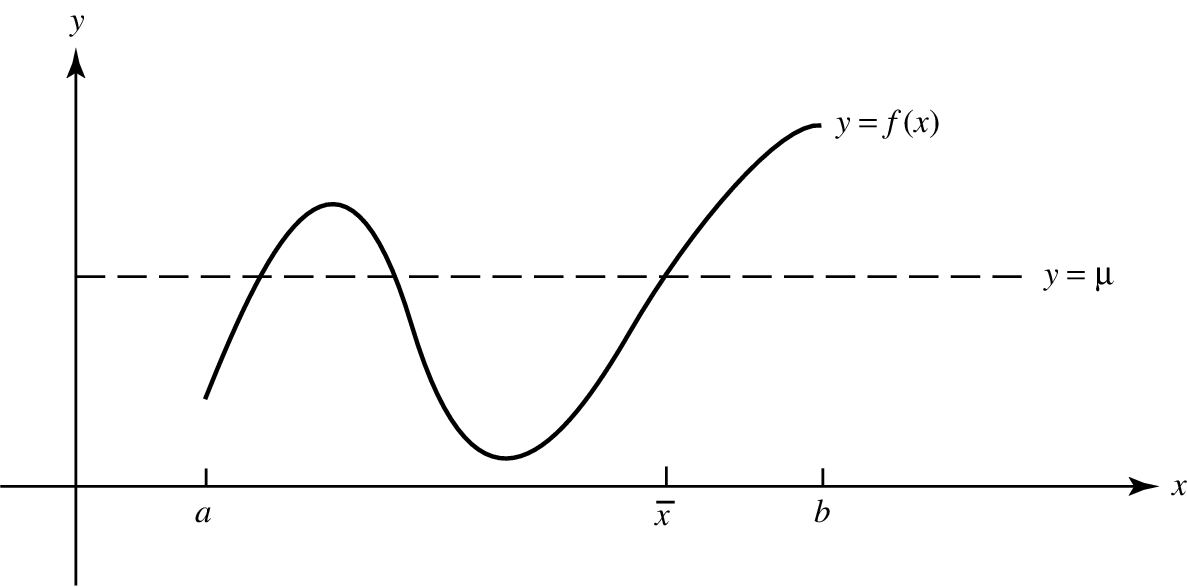
\includegraphics[width=4in,height=2in]{png/fig020205.png}
\end{center}
 \vskip6pt
 \refstepcounter{figure}
 \centerline{\bf Figure \thefigure} \label{figure:2.2.5}
 \vskip12pt

\proof
Suppose that  $f(a)<\mu<f(b)$.  The set
$$
S=\set{x}{a\le x\le b \mbox{\quad and }\ f(x)\le\mu}
$$
is bounded and nonempty. Let $c=\sup S$.
We will show that $f(c)=\mu$.
If $f(c)>\mu$, then $c>a$ and, since $f$ is
continuous at $c$, there is an $\epsilon>0$ such that
$f(x)>\mu$ if $c-\epsilon<x\le c$ (Exercise~\ref{exer:2.2.15}).
Therefore,
$c-\epsilon$ is an upper bound for $S$, which contradicts
the definition of $c$ as the  supremum of $S$. If
$f(c) <\mu$, then $c<b$ and there is an
$\epsilon>0$ such that $f(x)<\mu$ for $c\le
x<c+\epsilon$, so $c$ is not an upper bound
for $S$. This is also a contradiction. Therefore,
$f(c)=\mu$.

The proof for the case where $f(b)<\mu<f(a)$ can be obtained by
applying this result to $-f$.
\bbox

\boxit{Uniform Continuity}

Theorem~\ref{thmtype:2.2.2} and Definition~\ref{thmtype:2.2.3} imply that a

function $f$ is continuous on a subset $S$ of its domain if for each
$\epsilon>0$ and each $x_0$ in $S$, there is a $\delta>0$, {\it which
may depend upon $x_0$ as well as $\epsilon$}, such that
$$
|f(x)-f(x_0)|<\epsilon\mbox{\quad if \quad} |x-x_0|<\delta
\mbox{\quad and \quad} x\in D_f.
$$

The next definition introduces another kind of continuity on a set $S$.

\begin{definition}\label{thmtype:2.2.11}
A function $f$ is  {\it uniformly continuous\/} on a subset
$S$
of its domain if, for every $\epsilon >0$, there is a $\delta>0$ such
that
$$
|f(x)-f(x')|<\epsilon\mbox{\ whenever }\ |x-x'|<\delta
\mbox{\ and }\ x,x'\in S.
\eqno{\bbox}
$$
\end{definition}

We emphasize that in this definition $\delta$ depends only on $\epsilon$
and $S$ and not on the particular choice of $x$ and $x'$, provided
that they are both in $S$.

\enlargethispage{\baselineskip}
\begin{example}\label{example:2.2.13}\rm   The function
$$
f(x)=2x
$$

\newpage
\noindent
is uniformly continuous on $(-\infty,\infty)$, since
$$
|f(x)-f(x')|=2|x-x'|<\epsilon\mbox{\quad if \quad} |x-x'|<\epsilon/2.
$$
\end{example}

\begin{example}\label{example:2.2.14}\rm   If $0<r<\infty$, then the function
$$
g(x)=x^2
$$
is uniformly continuous on $[-r,r]$. To see this, note that
$$
|g(x)-g(x')=|x^2-(x')^2|=|x-x'|\,|x+x'|\le2r |x-x'|,
$$
so
$$
|g(x)-g(x')|<\epsilon\mbox{\quad if \quad}\
|x-x'|<\delta=\frac{\epsilon}{
2r}\mbox{\quad and }-r\le x,x'\le r.
\eqno{\bbox}
$$
\end{example}

Often a concept is clarified by considering its negation: a function
$f$ is {\it not\/} uniformly continuous on $S$ if there is an
$\epsilon_0>0$ such that if  $\delta$ is any positive number,
there are points
$x$ and $x'$ in $S$ such that
$$
|x-x'|<\delta\mbox{\quad but\quad} |f(x)-f(x')|\ge\epsilon_0.
$$

\begin{example}\label{example:2.2.15}\rm The function $g(x)=x^2$
is uniformly continuous on $[-r,r]$ for any finite $r$
(Example~\ref{example:2.2.14}), but not  on
$(-\infty,\infty)$. To see this, we will show that if $\delta>0$
there are real numbers  $x$ and $x'$  such that
$$
|x-x'|=\delta/2\mbox{\quad and \quad}|g(x)-g(x')|\ge1.
$$
To this end, we write
$$
|g(x)-g(x')|=|x^2-(x')^2|=|x-x'|\,|x+x'|.
$$
If  $|x-x'|=\delta/2$ and $x,x'>1/\delta$, then
$$
|x-x'|\,|x+x'|
>\frac{\delta}{2}\left(\frac{1}{
\delta}+\frac{1}{\delta}\right)=1.
$$
\end{example}

\begin{example}\label{example:2.2.16}\rm   The function
$$
f(x)=\cos \frac{1}{ x}
$$
is continuous on $(0,1]$ (Exercise~\ref{exer:2.2.23}\part{i}).
However, $f$ is not uniformly continuous on $(0,1]$, since
$$
\left|f\left(\frac{1}{ n\pi}\right)-f\left(\frac{1}{(n+1)\pi}\right)\right|
=2,\quad n=1,2, \dots.
\eqno{\bbox}
$$
\end{example}

Examples~\ref{example:2.2.15} and \ref{example:2.2.16} show that a function
may be continuous but not uniformly continuous on an interval. The
next theorem shows that this cannot happen if the interval is closed
and bounded, and therefore compact.

\begin{theorem}\label{thmtype:2.2.12}

If $f$ is continuous on a closed and bounded interval $[a,b],$
then $f$ is uniformly continuous on $[a,b].$
\end{theorem}

\proof
Suppose that $\epsilon>0$. Since $f$ is continuous on $[a,b]$,
for each $t$ in $[a,b]$  there is a positive number
$\delta_{t}$ such that
\begin{equation}\label{eq:2.2.10}
|f(x)-f(t)|<\frac{\epsilon}{2}
\mbox{\quad if \quad}
|x-t|<2\delta_{t}
\mbox{\quad and \quad} x\in[a,b].
\end{equation}
If $I_{t}=(t-\delta_{t
},t+\delta_{t})$, the collection
$$
{\mathcal H}=\set{I_{t}}{t\in [a,b]}
$$
is an open covering of $[a,b]$. Since $[a,b]$ is compact, the
Heine--Borel theorem implies that there are finitely many points
$t_1$, $t_2$, \dots, $t_n$ in
$[a,b]$ such that $I_{t_1}$, $I_{t_2}$, \dots, $I_{t_n}$ cover
$[a,b]$. Now define
\begin{equation}\label{eq:2.2.11}
\delta=\min\{\delta_{t_1},\delta_{t_2}, \dots,\delta_{t_n}\}.
\end{equation}
We will show  that if
\begin{equation} \label{eq:2.2.12}
|x-x'|<\delta \mbox{\quad and \quad}x,x'\in [a,b],
\end{equation}
then
$|f(x)-f(x')|<\epsilon$.

From the triangle inequality,
\begin{equation} \label{eq:2.2.13}
\begin{array}{rcl}
|f(x)-f(x')|\ar =
|\left(f(x)-f(t_r)\right)+\left(f(t_r)-f(x')\right)|\\
\ar\le  |f(x)-f(t_r)|+|f(t_r)-f(x')|.
\end{array}
\end{equation}
Since $I_{t_1}$, $I_{t_2}$, \dots, $I_{t_n}$ cover $[a,b]$, $x$ must
be in one of
these intervals.  Suppose that
$x\in I_{t_r}$; that is,
\begin{equation} \label{eq:2.2.14}
|x-t_r|<\delta_{t_r}.
\end{equation}
From \eqref{eq:2.2.10} with $t=t_r$,
\begin{equation} \label{eq:2.2.15}
|f(x)-f(t_r)|<\frac{\epsilon}{2}.
\end{equation}
From \eqref{eq:2.2.12}, \eqref{eq:2.2.14}, and the triangle inquality,
$$
|x'-t_r|=|(x'-x)+(x-t_r)|\le
 |x'-x|+|x-t_r|<\delta+\delta_{t_r}\le2\delta_{t_r}.
$$
Therefore, \eqref{eq:2.2.10} with $t=t_r$ and $x$ replaced by
$x'$ implies that
$$
|f(x')-f(t_r)|<\frac{\epsilon}{2}.
$$
This, \eqref{eq:2.2.13}, and \eqref{eq:2.2.15} imply  that
$|f(x)-f(x')|<\epsilon$.
\bbox

This proof again shows the utility of the Heine--Borel theorem, which
allowed us to define $\delta$ in \eqref{eq:2.2.11} as the smallest of a {\it
finite\/} set of positive numbers, so that $\delta$ is sure to be
positive. (An infinite set of positive numbers may fail to have a
smallest positive member; for example, consider the open interval
$(0,1)$.)

\begin{corollary}\label{thmtype:2.2.13}
If $f$ is continuous on a set $T,$ then  $f$ is  uniformly continuous
on any finite closed interval contained in $T.$
\end{corollary}

\newpage

Applied to Example~\ref{example:2.2.16}, Corollary~\ref{thmtype:2.2.13} implies
that the function $g(x)=\cos1/x$ is uniformly continuous on
$[\rho,1]$ if $0<\rho<1$.

\boxit{More About Monotonic Functions}
Theorem~\ref{thmtype:2.1.9} implies that if $f$ is monotonic on an
interval $I$, then $f$ is either continuous or has a jump
discontinuity at each $x_0$ in $I$. This and Theorem~\ref{thmtype:2.2.10}
provide the key to the proof of the following theorem.

\begin{theorem}\label{thmtype:2.2.14}
If $f$ is monotonic and nonconstant on $[a,b],$ then $f$ is continuous
on $[a,b]$ if and only if its range $R_f=\set{f(x)}{x\in[a,b]}$ is the
closed interval with endpoints $f(a)$ and $f(b).$
\end{theorem}

\proof
We assume that  $f$ is nondecreasing, and
leave the case where $f$ is nonincreasing to you
(Exercise~\ref{exer:2.2.34}).
Theorem~\ref{thmtype:2.1.9}\part{a}
implies that the set $\widetilde R_f=\set{f(x)}{x\in(a,b)}$
is a subset of the open interval $(f(a+),f(b-))$.  Therefore,
\begin{equation} \label{eq:2.2.16}
R_f=\{f(a)\}\cup\widetilde
R_f\cup\{f(b)\}\subset\{f(a)\}\cup(f(a+),f(b-))\cup\{f(b)\}.
\end{equation}
Now
suppose that $f$ is continuous on $[a,b]$. Then $f(a)=f(a+)$,
$f(b-)=f(b)$,
so \eqref{eq:2.2.16} implies that
$R_f\subset[f(a),f(b)]$. If $f(a)<\mu<f(b)$, then
Theorem~\ref{thmtype:2.2.10}  implies that $\mu=f(x)$ for some $x$
in $(a,b)$.  Hence, $R_f=[f(a),f(b)]$.

For the converse, suppose that
$R_f=[f(a),f(b)]$. Since $f(a)\le f(a+)$ and $f(b-)\le f(b)$,
\eqref{eq:2.2.16}  implies that $f(a)=f(a+)$ and $f(b-)=f(b)$.
 We know from
Theorem~\ref{thmtype:2.1.9}\part{c}
that if $f$ is nondecreasing and $a<x_0<b$, then
$$
f(x_0-)\le f(x_0)\le f(x_0+).
$$
If either of these inequalities  is strict,  $R_f$
cannot be an interval. Since  this contradicts our assumption,
$f(x_0-)=f(x_0)=f(x_0+)$. Therefore, $f$ is continuous at $x_0$
(Exercise~\ref{exer:2.2.2}).
We can now conclude that $f$ is continuous on $[a,b]$.
\bbox

Theorem~\ref{thmtype:2.2.14} implies the following theorem.

\begin{theorem}\label{thmtype:2.2.15}
Suppose that $f$ is increasing and continuous on $[a,b],$ and let
$f(a)=c$ and $f(b)=d.$ Then there is a unique function $g$ defined on
$[c,d]$ such that
\begin{equation}\label{eq:2.2.17}
g(f(x))=x,\quad a\le x\le b,
\end{equation}
and
\begin{equation}\label{eq:2.2.18}
f(g(y))=y,\quad c\le y\le d.
\end{equation}
Moreover$,$ $g$ is continuous and increasing on $[c,d].$
\end{theorem}

\proof
We first show that there is a function $g$ satisfying \eqref{eq:2.2.17}
and \eqref{eq:2.2.18}.
Since $f$ is continuous, Theorem~\ref{thmtype:2.2.14} implies that for
each
$y_0$ in $[c,d]$ there is an $x_0$ in $[a,b]$ such that
\begin{equation}\label{eq:2.2.19}
f(x_0)=y_0,
\end{equation}

\newpage
\noindent
and, since $f$ is increasing, there is only one such $x_0$. Define
\begin{equation}\label{eq:2.2.20}
g(y_0)=x_0.
\end{equation}
The definition of $x_0$ is illustrated in Figure~\ref{figure:2.2.6}: with
$[c,d]$ drawn on the $y$-axis, find the intersection of the line
$y=y_0$ with the curve $y=f(x)$ and drop a vertical from the
intersection to the $x$-axis to find $x_0$.

 \vspace*{12pt}
\begin{center}
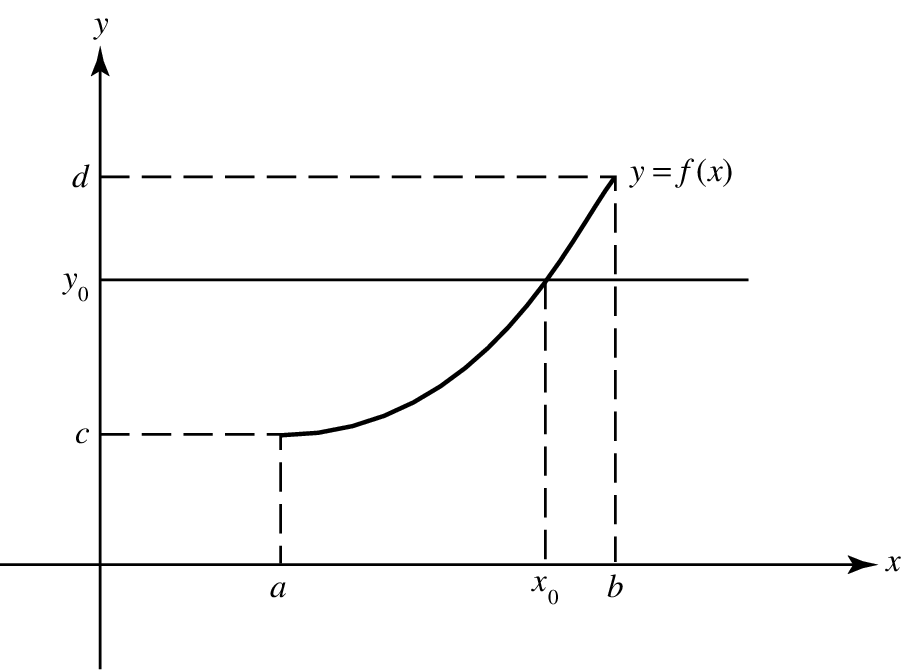
\includegraphics[width=3.1in,height=2.25in]{png/fig020206.png}
\end{center}
 \vskip6pt
 \refstepcounter{figure}
 \centerline{\bf Figure \thefigure} \label{figure:2.2.6}
 \vskip12pt

Substituting \eqref{eq:2.2.20} into \eqref{eq:2.2.19} yields
$$
f(g(y_0))=y_0,
$$
and substituting \eqref{eq:2.2.19} into \eqref{eq:2.2.20} yields
$$
g(f(x_0))=x_0.
$$
Dropping the subscripts in these two equations yields \eqref{eq:2.2.17}
and \eqref{eq:2.2.18}.

The uniqueness of  $g$
follows from our assumption that $f$ is increasing, and therefore only
one value of $x_0$ can satisfy \eqref{eq:2.2.19} for each $y_0$.

To see that $g$ is increasing, suppose that $y_1<y_2$ and let $x_1$
and $x_2$ be the points in $[a,b]$ such that $f(x_1)=y_1$ and
$f(x_2)=y_2$. Since  $f$ is increasing, $x_1<x_2$. Therefore,
$$
g(y_1)=x_1<x_2=g(y_2),
$$
so $g$ is increasing.
Since $R_g=\set{g(y)}{y\in[c,d]}$ is the interval $[g(c),g(d)]=[a,b]$,
Theorem~\ref{thmtype:2.2.14} with $f$ and $[a,b]$ replaced by $g$ and
$[c,d]$ implies that $g$ is continuous on $[c,d]$.
\bbox

The function $g$ of Theorem~\ref{thmtype:2.2.15} is  the {\it
inverse\/} of $f$,  denoted by $f^{-1}$. Since \eqref{eq:2.2.17} and
\eqref{eq:2.2.18} are symmetric in $f$ and $g$, we can also regard $f$ as
the inverse of $g$, and denote it by $g^{-1}$.

\begin{example}\label{example:2.2.17}\rm   If
$$
f(x)=x^2,\quad 0\le x\le R,
$$
then
$$
f^{-1}(y)=g(y)=\sqrt{y},\quad 0\le y\le R^2.
$$
\end{example}

\begin{example}\label{example:2.2.18}\rm   If
$$
f(x)=2x+4,\quad 0\le x\le2,
$$
then
$$
f^{-1}(y)=g(y)=\frac{y-4}{2},\quad 4\le y\le8.
$$
\end{example}

\exercises
\begin{exerciselist}

\item\label{exer:2.2.1} Prove Theorem~\ref{thmtype:2.2.2}.

\item\label{exer:2.2.2} Prove that a function $f$ is continuous at $x_0$
if and only if
$$
\lim_{x\to x_0-}f(x)=\lim_{x\to x_0+}f(x)=f(x_0).
$$

\item\label{exer:2.2.3}
Determine whether $f$ is continuous or discontinuous
from the right or left at~$x_0$.

\begin{tabular}{ll}
\part{a} $f(x)=\sqrt{x}\quad(x_0=0)$&
\part{b} $f(x)=\sqrt{x}\quad(x_0>0)$ \\
\part{c} $f(x)=\dst\frac{1}{x}\quad(x_0=0)$&
\part{d} $f(x)=x^2\quad(x_0\mbox{ arbitrary})$
\end{tabular}

\begin{tabular}{l}
\part{e} $f(x)=\left\{\casespace\begin{array}{ll} x\sin1/x,&x\ne0,\\
 1,&x=0\end{array}\right.\quad (x_0=0)$\\[4\jot]
\part{f} $f(x)=\left\{\casespace\begin{array}{ll} x\sin1/x,&x\ne0\\
 0,&x=0\end{array}\right.\quad (x_0=0)$\\[2\jot]
\part{g} $f(x)=\left\{\casespace\begin{array}{ll}\dst\frac{x+|x|(1+x)}{
x}\sin
\dst\frac{1}{ x},&x\ne0\\ 1,&x=0\end{array}\right.\quad
(x_0=0)$
\end{tabular}

\item\label{exer:2.2.4} Let $f$ be defined on $[0,2]$ by
$$
f(x)=\left\{\casespace\begin{array}{ll} x^2,&0\le x<1,\\[2\jot]
x+1,&1\le x\le2.\end{array}\right.
$$
On which of the following intervals is $f$ continuous according to
Definition~\ref{thmtype:2.2.3}:
$[0,1)$, $(0,1)$, $(0,1]$, $[0,1]$,
$[1,2)$, $(1,2)$, $(1,2]$, $[1,2]$?

\item\label{exer:2.2.5}  Let
$$
g(x)=\frac{\sqrt{x}}{ x-1}.
$$
On which of the following intervals is $g$ continuous according to
Definition~\ref{thmtype:2.2.3}: $[0,1)$, $(0,1)$, $(0,1]$, $[1,\infty)$,
$(1,\infty)$?

\item\label{exer:2.2.6}  Let
$$
f(x)=\left\{\casespace\begin{array}{rl} $-1$&\mbox{if $x$ is
irrational},\\[2\jot]
$1$&\mbox{if $x$ is rational}.\end{array}\right.
$$
Show that $f$ is not continuous anywhere.

\item\label{exer:2.2.7}
Let $f(x)=0$ if $x$ is irrational and $f(p/q)=1/q$
if $p$ and $q$ are positive integers with no common factors. Show that
$f$ is discontinuous at every rational and continuous at every
irrational on $(0,\infty)$.

\item\label{exer:2.2.8} Prove: If $f$ assumes only finitely many values,
then $f$ is continuous at a point $x_0$ in $D_f^0$ if and only if
$f$ is constant on some interval $(x_0-\delta, x_0+\delta)$.

\item\label{exer:2.2.9}
 The {\it characteristic function\/} $\psi_T$ of
a set $T$ is defined by
$$
\psi_T(x)=\left\{\casespace\begin{array}{ll} 1,&x\in T,\\[2\jot]
0,&x\not\in T.\end{array}\right.
$$
Show that $\psi_T$ is continuous at a point $x_0$ if and only if $x_0\in
T^0\cup (T^c)^0$.

\item\label{exer:2.2.10} Prove: If $f$ and $g$ are continuous on $(a,b)$
and $f(x)= g(x)$ for every $x$ in a dense subset
(Definition~\ref{thmtype:1.1.5}) of $(a,b)$, then $f(x)=g(x)$ for
all
$x$ in $(a,b)$.

\item\label{exer:2.2.11} Prove that the function $g(x)=\log x$ is
continuous on $(0,\infty)$. Take the following properties as given.
\begin{alist}
\item % (a)
 $\lim_{x\to 1}g(x)=0$.
\item % (b)
 $g(x_1)+g(x_2)=g(x_1x_2)$ if $x_1,x_2>0$.
\end{alist}

\item\label{exer:2.2.12} Prove that the function $f(x)=e^{ax}$ is
continuous on $(-\infty,\infty)$. Take the following properties as
given.

\begin{alist}
\item % (a)
$\lim_{x\to 0}f(x)=1$.
\item % (b)
 $f(x_1+x_2)=f(x_1)f(x_2),\quad -\infty<x_1,x_2<\infty$.
\end{alist}
\item\label{exer:2.2.13}
\begin{alist}
\item % (a)
 Prove that the functions $\sinh x$ and $\cosh x$ are
continuous for all $x$.
\item % (b)
 For what values of $x$ are $\tanh x$ and $\coth x$ continuous?
\end{alist}

\item\label{exer:2.2.14} Prove that the functions $s(x)=\sin x$ and
$c(x)=\cos x$ are continuous on $(-\infty,\infty)$. Take the following
properties as given.

\begin{alist}
\item % (a)
$\lim_{x\to 0}c(x)=1$.
\item % (b)
$c(x_1-x_2)=c(x_1)c(x_2)+s(x_1)s(x_2),\quad-\infty<x_1, x_2
<\infty$.
\item % (c)
 $s^2(x)+c^2(x)=1,\quad-\infty<x<\infty$.
\end{alist}

\item\label{exer:2.2.15}
\begin{alist}
\item % (a)
 Prove:  If $f$ is continuous at $x_0$ and $f(x_0)>\mu$, then
$f(x)>\mu$ for all $x$ in some neighborhood of $x_0$.
\item % (b)
State a result analogous to \part{a} for the case where $f(x_0)<\mu$.
\item % (c)
 Prove:  If $f(x)\le\mu$ for all $x$ in $S$ and $x_0$ is a
limit point of $S$ at which $f$ is continuous, then $f(x_0)\le\mu$.
\item % (d)
 State results analogous to  \part{a}, \part{b}, and \part{c} for
the case where $f$ is continuous from the  right or left at
$x_0$.
\end{alist}

\item\label{exer:2.2.16} Let $|f|$ be the function whose value at each $x$
in $D_f$ is $|f(x)|$. Prove: If $f$ is continuous at $x_0$, then so is
$|f|$. Is the converse true?

\item\label{exer:2.2.17} Prove: If $f$ is monotonic on $[a,b]$, then $f$
is piecewise continuous on $[a,b]$ if and only if $f$ has only
finitely many discontinuities in $[a,b]$.

\item\label{exer:2.2.18} Prove Theorem~\ref{thmtype:2.2.5}.

\item\label{exer:2.2.19}
\begin{alist}
\item % (a)
  Show that if $f_1$, $f_2$, \dots, $f_n$ are continuous on a set
$S$ then so are $f_1+f_2+\cdots+f_n$ and $f_1f_2\cdots f_n$.
\item % (b)
 Use \part{a} to show that a rational function is continuous
for all values of $x$ except the zeros of its denominator.
\end{alist}

\item\label{exer:2.2.20}
\begin{alist}
\item % (a)
Let $f_1$ and $f_2$ be continuous at $x_0$ and define
$$
F(x)=\max\left(f_1(x),f_2(x)\right).
$$
Show that $F$ is continuous at $x_0$.
\item % (b)
 Let $f_1$, $f_2$, \dots, $f_n$ be continuous at $x_0$ and define
$$
F(x)=\max\left(f_1(x),f_2(x), \dots,f_n(x)\right).
$$
Show that $F$ is continuous at $x_0$.
\end{alist}

\item\label{exer:2.2.21} Find the domains of $f\circ g$ and $g\circ f$.

\begin{tabular}[t]{@{}p{168pt}@{}p{168pt}}
\part{a} $f(x)=\sqrt{x},\quad g(x)=1-x^2$&
\part{b} $f(x)=\log x,\quad g(x)=\sin x$\\[2\jot]
\part{c} $f(x)=\dst\frac{1}{1-x^2},\quad g(x)=\cos x$&
\part{d} $f(x)=\sqrt{x},\quad g(x)=\sin2x$
\end{tabular}

\item\label{exer:2.2.22}
\begin{alist}
\item % (a)
Suppose that $y_0=\lim_{x\to x_0} g(x)$ exists and is an interior
point of $D_f$, and that $f$ is continuous at  $y_0$.
 Show that
$$
\lim_{x\to x_0} (f\circ g)(x)=f(y_0).
$$
\item % (b)
 State an analogous result for limits from the right.
\item % (c)
 State an analogous result for limits from the left.
\end{alist}

\item\label{exer:2.2.23} Use Theorem~\ref{thmtype:2.2.7} to find all points
$x_0$ at which the following functions are continuous.

\begin{tabular}[t]{@{}p{112pt}@{}p{112pt}@{}p{112pt}}
 \part{a} $\sqrt{1-x^2}$&\part{b} $\sin e^{-x^2}$&\part{c} $\log(1+\sin
x)$\\\\
 \part{d} $e^{-1/(1-2x)}$&\part{e} $\sin\dst\frac{1}{(x-1)^2}$
&\part{f} $\sin\dst{\left(\frac{1}{\cos x}\right)}$\\\\
 \part{g} $(1-\sin^2x)^{-1/2}$&\part{h} $\cot(1-e^{-x^2})$&\part{i} $\cos
\dst\frac{1}{ x}$\\
\end{tabular}

\item\label{exer:2.2.24} Complete the proof of Theorem~\ref{thmtype:2.2.9}
by showing that there is an $x_2$ such that $f(x_2)~=~\beta$.

\newpage

\item\label{exer:2.2.25} Prove: If $f$ is nonconstant and continuous on an
interval $I$, then the set $S=\set{y}{y=f(x), x\in I}$ is an interval.
Moreover, if $I$ is a finite closed interval, then so is $S$.

\item\label{exer:2.2.26} Suppose that $f$ and $g$ are defined on
$(-\infty,\infty)$, $f$ is increasing, and $f\circ g$ is continuous
on $(-\infty,\infty)$. Show that $g$ is continuous on
$(-\infty,\infty)$.

\item\label{exer:2.2.27}  Let $f$ be continuous on $[a,b)$, and define
$$
F(x)=\max_{a\le t\le x}f(t),\quad a\le x<b.
$$
(How do we know  that $F$ is well defined?)  Show that $F$ is
continuous on
$[a,b)$.

\item\label{exer:2.2.28} Let $f$ and $g$ be uniformly continuous on an
interval $S$.

\begin{alist}
\item % (a)
Show that $f+g$ and $f-g$ are uniformly continuous on $S$.
\item % (b)
 Show that $fg$ is uniformly continuous on $S$ if $S$ is
compact.
\item % (c)
 Show that $f/g$ is uniformly continuous on $S$ if $S$ is
compact and $g$ has no zeros in $S$.
\item % (d)
 Give examples showing that the conclusion of \part{b} and \part{c} may
fail to hold if $S$ is not compact.
\item % (e)
 State additional conditions on $f$ and $g$ which guarantee
that $fg$ is uniformly continuous on $S$ even if $S$ is not compact.  Do
the same for $f/g$.
\end{alist}

\item\label{exer:2.2.29} Suppose that $f$ is uniformly continuous on a set
$S$, $g$ is uniformly continuous on a set $T$, and $g(x)\in S$ for
every $x$ in $T$. Show that $f\circ g$ is uniformly continuous on $T$.

\item\label{exer:2.2.30}
\begin{alist}
\item % (a)
 Prove:  If $f$ is uniformly continuous on disjoint closed
intervals $I_1$, $I_2$, \dots, $I_n$, then $f$ is uniformly continuous
on
$\bigcup^n_{j=1}I_j$.
\item % (b)
 Is \part{a} valid without the word ``closed''?
\end{alist}

\item\label{exer:2.2.31}
\begin{alist}
\item % (a)
 Prove:  If $f$ is uniformly continuous on a bounded open
interval $(a,b)$, then $f(a+)$ and $f(b-)$ exist and are finite.
\hint{See Exercise~$\ref{exer:2.1.38}.$}
\item % (b)
 Show that the conclusion in \part{a} does not follow if
$(a,b)$ is unbounded.
\end{alist}

\item\label{exer:2.2.32} Prove: If $f$ is continuous on $[a,\infty)$ and
$f(\infty)$ exists (finite), then $f$ is uniformly continuous on
$[a,\infty)$.

\item\label{exer:2.2.33}
Suppose that $f$ is defined on $(-\infty,\infty)$
and has the following properties.
$$
\mbox{\part{i}\quad} \lim_{x\to 0}f(x)=1
\mbox{\, and \,}
\mbox{\part{ii}\quad} f(x_1+x_2)=f(x_1)f(x_2),\quad
-\infty<x_1,x_2<\infty.
$$
 Prove:
\begin{alist}
\item % (a)
$f(x)>0$ for all $x$.
\item % (b)
 $f(rx)=[f(x)]^r$ if $r$ is rational.
\item % (c)
 If $f(1)=1$ then $f$ is constant.

\newpage
\item % (d)
 If $f(1)=\rho>1$, then $f$ is increasing,
$$
\lim_{x\to
\infty}f(x)=\infty,\mbox{\quad and \quad}
\lim_{x\to-\infty}f(x)=0.
$$
(Thus,
$f(x)=e^{ax}$ has these properties if $a>0$.)
\end{alist}
\hint{See Exercises~$\ref{exer:2.2.10}$ and $\ref{exer:2.2.12}.$}

\item\label{exer:2.2.34} Prove Theorem~\ref{thmtype:2.2.14} in the case where
$f$ is nonincreasing.

\label{sectionend:\thesection}
\end{exerciselist}


\currentpdfbookmark{Differentiable Functions of One Variable}{section:2.3}
\newsection{3}{Differential Calculus of Functions of One Variable
}{Differentiable Functions of One Variable}


\renewcommand{\thissection}{\sectiontitle{DIFFERENTIABLE FUNCTIONS OF
ONE VARIABLE}}
\thissection

\noindent
In calculus you studied differentiation, emphasizing rules for
calculating derivatives. Here we consider the theoretical properties
of differentiable functions. In doing this, we assume that you know
how
to differentiate elementary functions such as $x^n$, $e^x$, and $\sin
x$, and we will use such functions in examples.

\boxit{Definition of the Derivative}

\vspace*{-4ex}


\begin{definition}\label{thmtype:2.3.1}
A function $f$ is {\it differentiable\/}
at an interior point $x_0$ of its domain if the difference quotient
$$
\frac{f(x)-f(x_0)}{ x-x_0},\quad x\ne x_0,
$$
approaches a limit as $x$ approaches $x_0$, in which case the limit is
called the {\it derivative of $f$ at $x_0$\/}, and
is denoted by
$f'(x_0)$; thus,
\begin{equation}\label{eq:2.3.1}
f'(x_0)=\lim_{x\to x_0}\frac{f(x)-f(x_0)}{ x-x_0}.
\end{equation}
It is sometimes convenient to let $x=x_0+h$ and  write \eqref{eq:2.3.1}
as
$$
f'(x_0)=\lim_{h\to 0}\frac{f(x_0+h)-f(x_0)}{ h}.
\eqno{\bbox}
$$
\end{definition}

If $f$ is defined on an open set $S$, we say that
 $f$ is {\it differentiable on \/} $S$
if
$f$ is differentiable at every point of $S$.
If $f$ is differentiable on $S$, then $f'$ is a function on $S$. We
say that $f$ is {\it continuously differentiable\/}
 on $S$ if $f'$ is
continuous on $S$. If $f$ is differentiable on a neighborhood of
$x_0$, it is reasonable to ask if $f'$ is differentiable at $x_0$. If
so, we denote the derivative of $f'$ at $x_0$  by $f''(x_0)$.
This is the
{\it second derivative of $f$ at $x_0$\/},
and it is also denoted by
$f^{(2)}(x_0)$. Continuing inductively, if $f^{(n-1)}$ is defined on a
neighborhood of $x_0$, then the $n$th {\it derivative of $f$ at
$x_0$\/}, denoted by
$f^{(n)}(x_0)$, is the derivative of
$f^{(n-1)}$ at
$x_0$. For convenience we define the {\it zeroth
derivative\/} of
$f$ to be $f$ itself; thus
$$
f^{(0)}=f.
$$

We assume that you are familiar with the other standard notations for
derivatives; for example,
$$
f^{(2)}=f'',\quad f^{(3)}=f''',
$$
\newpage

\enlargethispage{\baselineskip}

\noindent
and so on, and
\vspace*{3pt}
$$
\frac{d^nf}{ dx^n}=f^{(n)}.
$$

\vspace*{3pt}

\begin{example}\label{example:2.3.1}\rm   If $n$ is a positive integer and
$$
f(x)=x^n,
$$
then
\vspace*{3pt}
$$
\frac{f(x)-f(x_0)}{ x-x_0}=\frac{x^n-x^n_0}{ x-x_0}
=\frac{x-x_0}{ x-x_0}\,\sum_{k=0}^{n-1} x^{n-k-1}x^k_0,
$$
\vspace*{3pt}
 so
\vspace*{3pt}
$$
f'(x_0)=\lim_{x\to x_0}\sum_{k=0}^{n-1} x^{n-k-1}x^k_0=nx^{n-1}_0.
$$
\vspace*{3pt}
Since this holds for every $x_0$, we drop the subscript and write
$$
f'(x)=nx^{n-1}\mbox{\quad or \quad}\frac{d}{ dx} (x^n)=nx^{n-1}.
\eqno{\bbox}
$$
\end{example}
\vspace*{3pt}

To derive differentiation formulas for elementary functions such as
$\sin x$, $\cos x$, and $e^x$ directly from Definition~\ref{thmtype:2.3.1}
requires estimates based on the properties of these functions. Since
this is done in calculus, we will not repeat it here.

\boxit{Interpretations of the Derivative}
If $f(x)$ is the position of a particle at time $x\ne x_0$, the
difference quotient
$$
\frac{f(x)-f(x_0)}{ x-x_0}
$$
is the  average velocity of the particle  between times $x_0$
and $x$. As $x$ approaches $x_0$, the average applies to shorter
and
shorter intervals. Therefore, it makes sense to regard the limit
\eqref{eq:2.3.1}, if it exists, as the particle's {\it instantaneous
velocity at time $x_0$\/}. This
interpretation may be useful even if
$x$
is not time, so we often regard $f'(x_0)$ as the {\it instantaneous
rate of change of $f(x)$ at $x_0$\/},
 regardless of the specific nature of the variable $x$.
The derivative also has a geometric interpretation. The equation of
the line through two points $(x_0,f(x_0))$ and
$(x_1,f(x_1))$ on the curve $y=f(x)$
(Figure~\ref{figure:2.3.1}) is
$$
y=f(x_0)+\frac{f(x_1)-f(x_0)}{ x_1-x_0} (x-x_0).
$$
\noindent
Varying $x_1$ generates lines through $(x_0,f(x_0))$ that
rotate into the line
\begin{equation}\label{eq:2.3.2}
y=f(x_0)+f'(x_0)(x-x_0)
\end{equation}

\newpage

\noindent
as $x_1$ approaches $x_0$. This is the {\it tangent\/}
 to the curve
$y=f(x)$ at the point $(x_0,f(x_0))$.
Figure~\ref{figure:2.3.2}
depicts the situation for various values of $x_1$.

 \vspace*{6pt}

\begin{center}
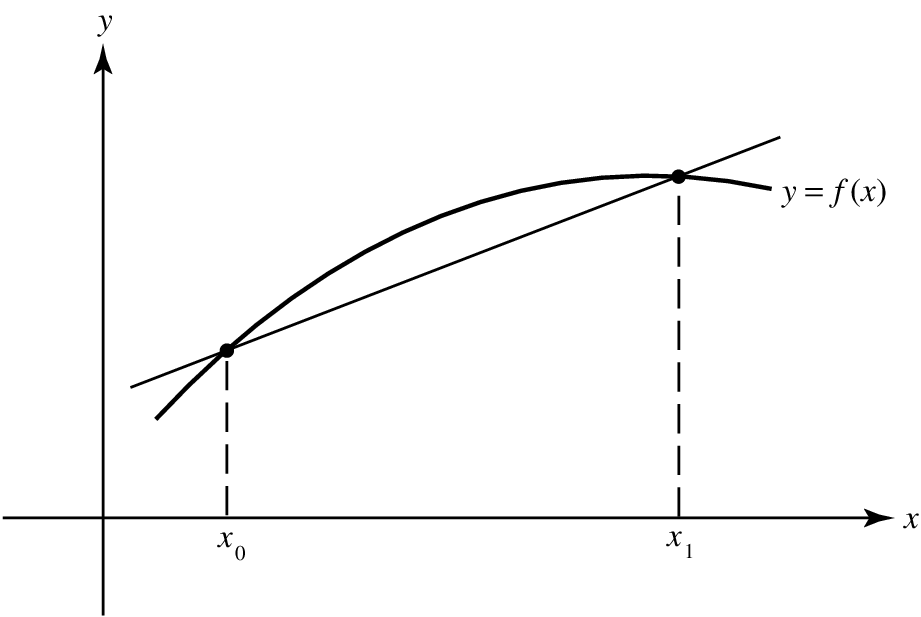
\includegraphics[width=3.1in,height=2.1in]{png/fig020301.png}
\end{center}
 \refstepcounter{figure}
 \centerline{\bf Figure \thefigure} \label{figure:2.3.1}

 \vspace*{12pt}
\begin{center}
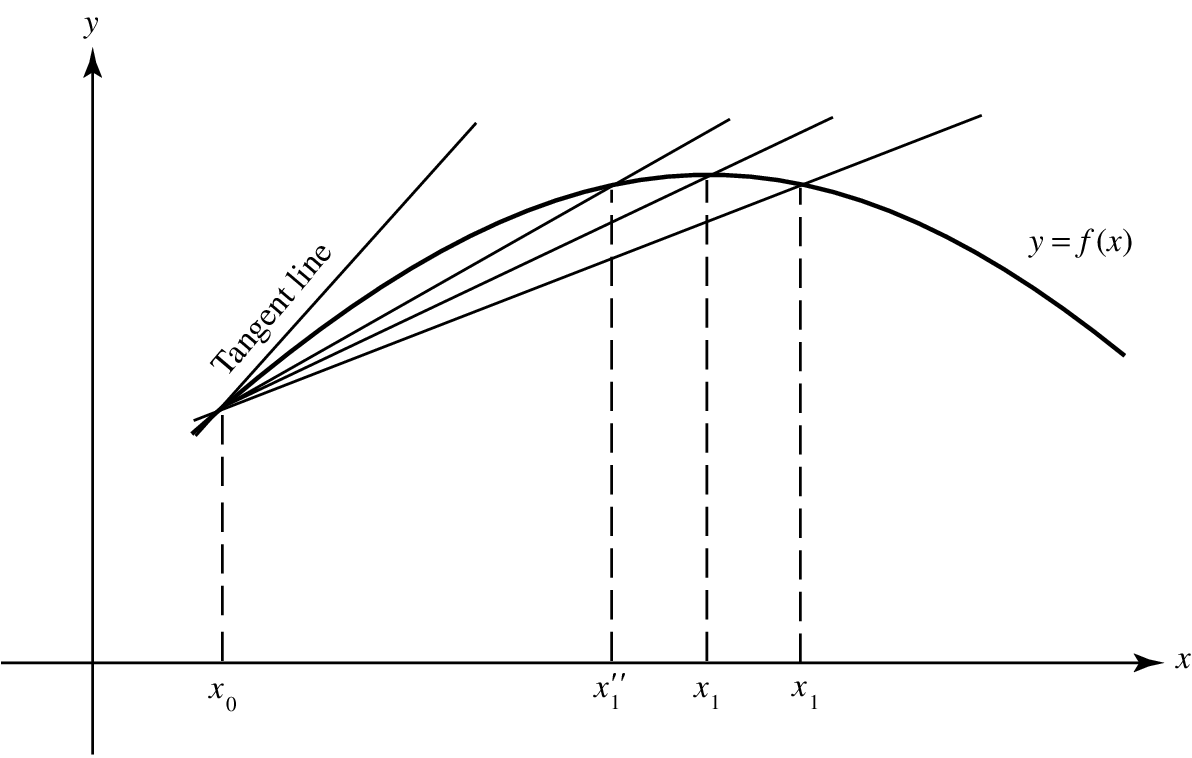
\includegraphics[width=4in,height=2.5in]{png/fig020302.png}
\end{center}
 \vskip6pt
 \refstepcounter{figure}
 \centerline{\bf Figure \thefigure} \label{figure:2.3.2}
 \vskip12pt

Here is a less intuitive definition of the tangent line:  If the
function
$$
T(x)=f(x_0)+m(x-x_0)
$$
approximates $f$ so well near $x_0$ that
$$
\lim_{x\to x_0}\frac{f(x)-T(x)}{ x-x_0}=0,
$$
 we say that the line $y=T(x)$ is {\it tangent to the curve
$y=f(x)$ at
$(x_0,f(x_0))$\/}.

\newpage
\noindent
This tangent line exists
if and only if
$f'(x_0)$ exists, in which case $m$ is uniquely determined by $m=f'(x_0)$
(Exercise~\ref{exer:2.3.1}). Thus, \eqref{eq:2.3.2} is the equation of the
tangent line.

We will use the following lemma to study differentiable functions.

\begin{lemma}\label{thmtype:2.3.2}
If $f$ is differentiable at $x_0,$ then
\begin{equation}\label{eq:2.3.3}
f(x)=f(x_0)+[f'(x_0)+E(x)](x-x_0),
\end{equation}
where $E$ is defined on a neighborhood of $x_0$ and
$$
\lim_{x\to x_0} E(x)=E(x_0)=0.
$$
\end{lemma}

\proof
  Define
\begin{equation} \label{eq:2.3.4}
E(x)=\left\{\casespace\begin{array}{ll}
\dst\frac{f(x)-f(x_0)}{ x-x_0}-
f'(x_0),&x\in D_f\mbox{ and }x\ne x_0,\\[2\jot]
0,&x=x_0.
\end{array}\right.
\end{equation}
Solving \eqref{eq:2.3.4} for $f(x)$ yields \eqref{eq:2.3.3} if $x\ne x_0$,
and \eqref{eq:2.3.3} is obvious if $x=x_0$.
Definition~\ref{thmtype:2.3.1}
implies that $\lim_{x\to x_0}E(x)=0$. We defined $E(x_0)=0$ to make
$E$ continuous at $x_0$.
\mbox{}\bbox

Since the right side of \eqref{eq:2.3.3} is continuous at $x_0$, so is the
left. This yields the following theorem.

\begin{theorem}\label{thmtype:2.3.3}
If $f$ is differentiable at $x_0,$ then $f$ is continuous at $x_0.$
\end{theorem}

\enlargethispage{100pt}
The converse of this theorem is false, since a function may be
continuous at a point without being differentiable at the point.

\begin{example}\label{example:2.3.2}\rm   The function
$$
f(x)=|x|
$$
can be written as
\begin{eqnarray}
f(x)\ar=\phantom{-}x,\quad x>0,\label{eq:2.3.5}\\ \arraytext{or
as}\nonumber\\ f(x)\ar=-x,\quad x<0\label{eq:2.3.6}.
\end{eqnarray}
From \eqref{eq:2.3.5},
\begin{eqnarray*}
f'(x)\ar=\phantom{-}1,\quad x>0,\\
\arraytext{and from \eqref{eq:2.3.6},}\\
f'(x)\ar=-1,\quad x<0.
\end{eqnarray*}
Neither \eqref{eq:2.3.5} nor \eqref{eq:2.3.6} holds throughout any
neighborhood of $0$, so neither can be used alone to calculate
$f'(0)$. In fact, since the one-sided limits
\begin{eqnarray}
\lim_{x\to 0+}\frac{f(x)-f(0)}{ x-0}\ar=\lim_{x\to 0+}\frac{x}{ x}
\hspace*{.6em}
\label{eq:2.3.7}\\
\arraytext{and}\nonumber \\
\lim_{x\to 0-}\frac{f(x)-f(0)}{ x-0}\ar=\lim_{x\to 0-}\frac{-x}{ x}=-1
\label{eq:2.3.8}
\end{eqnarray}

\newpage
\noindent
are different,
$$
\lim_{x\to 0}\frac{f(x)-f(0)}{ x-0}
$$
does not exist
   (Theorem~\ref{thmtype:2.1.6});
thus, $f$ is not
differentiable at $0$, even though it is continuous at $0$.
\end{example}

\boxit{Interchanging Differentiation and Arithmetic Operations}
The following theorem should be familiar from  calculus.

\begin{theorem}\label{thmtype:2.3.4}
If $f$ and $g$ are differentiable
at $x_0,$ then so are $f+g,$ $f-g,$ and $fg,$ with

\begin{alist}
\item % (a)
 $(f+g)'(x_0)=f'(x_0)+g'(x_0);$
\item % (b)
 $(f-g)'(x_0)=f'(x_0)-g(x_0);$
\item % (c)
 $(fg)'(x_0)=f'(x_0)g(x_0)+f(x_0)g'(x_0).$
\end{alist}
 The quotient $f/g$ is differentiable at $x_0$ if $g(x_0)\ne0,$ with
\begin{alist}
\setcounter{lcal}{3}
\item % (d)
$\dst{\left(\frac{f}{g}\right)' (x_0)=
\frac{f'(x_0)g(x_0)-f(x_0)g'(x_0)}{\left[g(x_0)\right]^2}}.$
\end{alist}
\end{theorem}

\proof The proof is accomplished by forming the appropriate
difference quotients and applying Definition~\ref{thmtype:2.3.1} and
Theorem~\ref{thmtype:2.1.4}. We will prove \part{c} and leave
the rest to you
(Exercises~\ref{exer:2.3.9}, \ref{exer:2.3.10}, and \ref{exer:2.3.11}).

 The trick is to add and subtract the right quantity in the numerator
of the difference quotient for $(fg)'(x_0)$; thus,
\begin{eqnarray*}
\frac{f(x)g(x)-f(x_0)g(x_0)}{ x-x_0}\ar=
\frac{f(x)g(x)-f(x_0)g(x)+f(x_0)g(x)-f(x_0)g(x_0)}{ x-x_0}\\
\ar=\frac{f(x)-f(x_0)}{ x-x_0} g(x)+f(x_0)\frac{g(x)-g(x_0)}{ x-x_0}.
\end{eqnarray*}
The difference quotients on the right approach $f'(x_0)$ and $g'(x_0)$
as $x$ approaches $x_0$, and $\lim_{x\to x_0}g(x)=g(x_0)$
   (Theorem~\ref{thmtype:2.3.3}).
This proves \part{c}.
\bbox

\boxit{The Chain Rule}
Here is the rule for differentiating a composite function.

\begin{theorem} [The Chain Rule]\label{thmtype:2.3.5}
Suppose that  $g$ is differentiable at $x_0$ and $f$ is differentiable at
$g(x_0).$ Then the composite function $h=f\circ g,$ defined by
$$
h(x)=f(g(x)),
$$
is differentiable at $x_0,$ with
$$
h'(x_0)=f'(g(x_0))g'(x_0).
$$
\end{theorem}

\newpage

\enlargethispage{-.5\baselineskip}

\proof
Since $f$ is differentiable at $g(x_0)$, Lemma~\ref{thmtype:2.3.2} implies
that
$$
f(t)-f(g(x_0))=[f'(g(x_0))+E(t)][t-g(x_0)],
$$
where
\begin{equation}\label{eq:2.3.9}
\lim_{t\to g(x_0)} E(t)=E(g(x_0))=0.
\end{equation}
Letting $t=g(x)$ yields
$$
f(g(x))-f(g(x_0))=[f'(g(x_0))+E(g(x))][g(x)-g(x_0)].
$$
Since $h(x)=f(g(x))$,  this implies that
\begin{equation}\label{eq:2.3.10}
\frac{h(x)-h(x_0)}{ x-x_0}=[f'(g(x_0))+E(g(x))]
\frac{g(x)-g(x_0)}{ x-x_0}.
\end{equation}
Since $g$ is continuous at $x_0$ (Theorem~\ref{thmtype:2.3.3}),
\eqref{eq:2.3.9} and Theorem~\ref{thmtype:2.2.7} imply that
$$
\lim_{x\to x_0} E(g(x))=E(g(x_0))=0.
$$
Therefore, \eqref{eq:2.3.10} implies that
$$
h'(x_0)=\lim_{x\to x_0}\frac{h(x)-h(x_0)}{ x-x_0}=f'(g(x_0))
g'(x_0),
$$
as stated.
\bbox

\begin{example}\label{example:2.3.3}\rm   If
$$
f(x)=\sin x\mbox{\quad and\quad} g(x)=\frac{1}{ x},\quad x\ne0,
$$
then
$$
h(x)=f(g(x))=\sin \frac{1}{ x},\quad x\ne0,
$$
and
$$
h'(x)=f'(g(x))g(x)=\left(\cos \frac{1}{ x}\right)
\left(-\frac{1}{ x^2}\right),\quad x\ne0.
\eqno{\bbox}
$$
\end{example}

It may seem reasonable to justify the chain rule by writing
\begin{eqnarray*}
\frac{h(x)-h(x_0)}{ x-x_0}\ar=\frac{f(g(x))-f(g(x_0))}{x-x_0}\\
\ar=\frac{f(g(x))-f(g(x_0))}{ g(x)-g(x_0)}\,
\frac{g(x)-g(x_0)}{ x-x_0}
\end{eqnarray*}
and arguing that
$$
\lim_{x\to x_0} \frac{f(g(x))-f(g(x_0))}{
g(x)-g(x_0)}=f'(g(x_0))
$$

\newpage
\noindent
(because $\lim_{x\to x_0} g(x)=g(x_0))$ and
\vspace*{3pt}
$$
\lim_{x\to x_0}\frac{g(x)-g(x_0)}{ x-x_0}=g'(x_0).
$$
\vspace*{3pt}
However, this is not a valid proof (Exercise~\ref{exer:2.3.13}).

\boxit{One-Sided Derivatives}
One-sided limits of difference quotients such as \eqref{eq:2.3.7} and
\eqref{eq:2.3.8} in Example~\ref{example:2.3.2} are called {\it one-sided\/} or
{\it right- and left-hand derivatives\/}.
 That is, if $f$ is defined on
 $[x_0,b)$, the {\it right-hand derivative of $f$ at $x_0$\/}
is defined to be
$$
f_+'(x_0)=\lim_{x\to x_0+}\frac{f(x)-f(x_0)}{ x-x_0}
$$
if the limit exists, while if $f$ is defined on  $(a,x_0]$,
the
{\it left-hand derivative of $f$ at $x_0$\/} is defined to be
$$
f_-'(x_0)=\lim_{x\to x_0-}\frac{f(x)-f(x_0)}{ x-x_0}
$$
if the limit exists. Theorem~\ref{thmtype:2.1.6} implies that $f$ is
differentiable at $x_0$ if and only if $f_+'(x_0)$ and $f_-'(x_0)$
exist and are equal, in which case
$$
f'(x_0)=f_+'(x_0)=f_-'(x_0).
$$

In Example~\ref{example:2.3.2}, $f_+'(0)=1$ and $f_-'(0)=-1$.
\vspace*{6pt}
\begin{example}\label{example:2.3.4}\rm   If

\begin{equation}\label{eq:2.3.11}
f(x)=\left\{\casespace\begin{array}{ll} x^3,&x\le0,\\[2\jot] x^2\sin
\dst\frac{1}{x},&x>0,
\end{array}\right.
\end{equation}
then
\begin{equation}\label{eq:2.3.12}
f'(x)=\left\{\casespace\begin{array}{ll} 3x^2,&x<0,\\[2\jot]
\dst{2x\sin\frac{1}{x}-\cos \frac{1}{
x}},&x>0.\end{array}\right.
\end{equation}
Since neither formula in \eqref{eq:2.3.11} holds for all $x$ in any
neighborhood of $0$, we cannot simply differentiate either to obtain
$f'(0)$; instead, we calculate
\begin{eqnarray*}
f_+'(0)\ar=\lim_{x\to 0+}\frac{x^2\sin\dst{\frac{1}{ x}}-0}{
x-0}=\lim_{x\to
0+} x\sin \frac{1}{ x}=0,\\[2\jot]
f_-'(0)\ar=\lim_{x\to0-}\frac{x^3-0}{ x-0}=\lim_{x\to 0-}x^2=0;
\end{eqnarray*}
\vspace*{3pt}
hence, $f'(0)=f_+'(0)=f_-'(0)=0$.
\bbox\end{example}

\newpage

This example shows that there is a difference between a one-sided
derivative and a one-sided limit of a derivative, since $f_+'(0)=0$,
but, from \eqref{eq:2.3.12}, $f'(0+)=\lim_{x\to 0+}f'(x)$ does not exist.
It also shows that a derivative may exist in a neighborhood of a point
$x_0$ ($=0$ in this case), but be discontinuous at $x_0$.

Exercise~\ref{exer:2.3.4} justifies the method used in
Example~\ref{example:2.3.4} to compute $f'(x)$ for $x\ne0$.

\begin{definition} \label{thmtype:2.3.6}
\begin{alist}
\item % (a)
We say that $f$ is {\it differentiable on the closed interval\/}
$[a,b]$ if $f$ is differentiable on the open interval $(a,b)$ and
$f_+'(a)$ and $f_-'(b)$  both exist.
\item % (b)
We say that $f$ is {\it continuously  differentiable on\/}
$[a,b]$ if $f$ is differentiable on  $[a,b]$, $f'$ is continuous
on $(a,b)$,
$f_+'(a)=f'(a+)$, and $f_-'(b)=f'(b-)$.
\end{alist}
\end{definition}

\boxit{Extreme Values}
We say that $f(x_0)$ is a {\it local extreme value\/} of $f$ if
there is a $\delta>0$ such that $f(x)-f(x_0)$ does not change sign on
\begin{equation}\label{eq:2.3.13}
(x_0-\delta,x_0+\delta)\cap D_f.
\end{equation}
More specifically, $f(x_0)$ is a {\it local maximum value\/} of $f$ if
\begin{equation}\label{eq:2.3.14}
f(x) \le f(x_0)
\end{equation}
or a {\it local minimum value\/} of $f$ if
\begin{equation}\label{eq:2.3.15}
f(x)\ge f(x_0)
\end{equation}
for all $x$ in the set \eqref{eq:2.3.13}. The point $x_0$ is called a {\it
local extreme point\/}  of $f$, or, more specifically, a
{\it local maximum\/} or {\it local minimum
point\/} of $f$.

 \vspace*{12pt}
\begin{center}
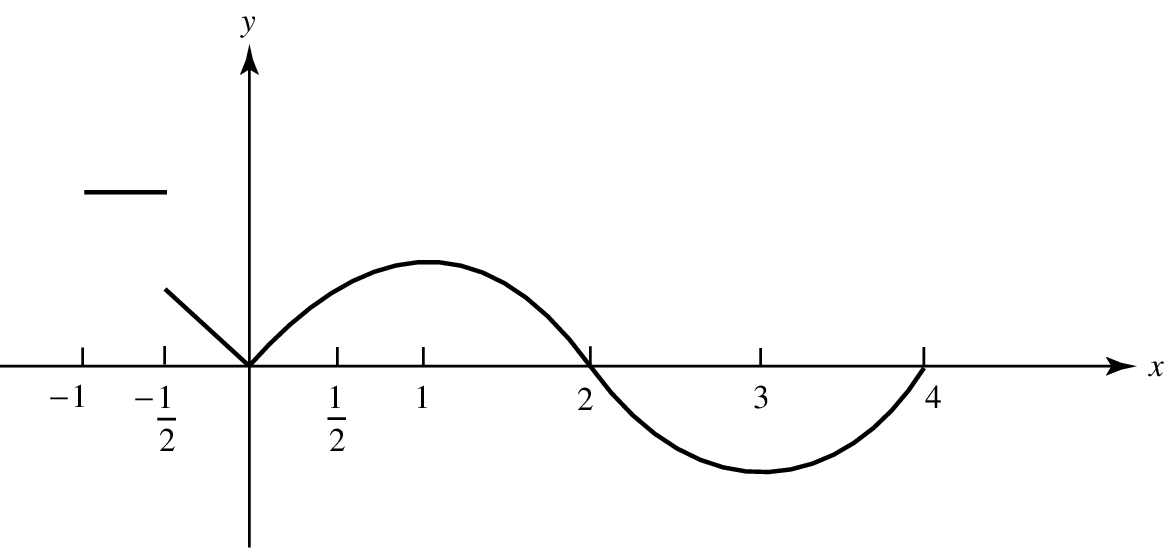
\includegraphics[width=4in,height=1.9in]{png/fig020303.png}
\end{center}
 \vskip6pt
 \refstepcounter{figure}
 \centerline{\bf Figure \thefigure} \label{figure:2.3.3}
 \vskip12pt

\newpage
\begin{example}\label{example:2.3.5}\rm   If
$$
f(x)=\left\{\casespace\begin{array}{cc} 1,&-1<x\le-\frac{1}{2}\\[2\jot]
 |x|,&-\frac{1}{2}<x\le \frac{1}{2},\\[2\jot]
\dst{\frac{1}{\sqrt{2}}\sin \frac{\pi
x}{2}},&\frac{1}{2}<x\le4\end{array}\right.
$$
\vskip4pt
\noindent(Figure~\ref{figure:2.3.3}), then $0$, $3$, and every
$x$ in
$(-1,-\frac{1}{2})$
are local minimum points of $f$, while $1$, $4$, and every $x$ in
$(-1,-\frac{1}{2}]$ are local maximum points.
\bbox\end{example}
\vskip4pt

It is geometrically plausible that if the curve $y=f(x)$ has a tangent
at a local extreme point of $f$, then the tangent must be horizontal;
that is, have zero slope. (For example, in Figure~\ref{figure:2.3.3}, see
$x=1$, $x=3$, and every $x$ in $(-1,-1/2)$.) The following theorem
shows that this must be so.
\vskip4pt

\begin{theorem}\label{thmtype:2.3.7}
If $f$ is differentiable at a local extreme point $x_0\in D_{f}^{0},$
then
$f'(x_0)=~0.$
\end{theorem}
\vskip4pt

\proof
We will show that $x_0$ is not a local extreme point of $f$ if
$f'(x_0)\ne0$. From Lemma~\ref{thmtype:2.3.2},
\begin{equation}\label{eq:2.3.16}
\frac{f(x)-f(x_0)}{ x-x_0}=f'(x_0)+E(x),
\end{equation}
where $\lim_{x\to x_0} E(x)=0$.  Therefore, if $f'(x_0)\ne0$,
there is a $\delta>0$ such that
$$
|E(x)|<|f'(x_0)|\mbox{\quad if\quad} |x-x_0|<\delta,
$$
and the right side of \eqref{eq:2.3.16} must have the same sign as
$f'(x_0)$ for $|x-x_0|<\delta$. Since the same is true of the left
side, $f(x)-f(x_0)$ must change sign in every neighborhood of $x_0$
(since $x-x_0$ does). Therefore, neither \eqref{eq:2.3.14} nor
\eqref{eq:2.3.15} can hold for all $x$ in any interval about $x_0$.
\bbox
\vskip4pt

If $f'(x_0)=0$, we say that $x_0$ is a {\it critical point\/} of $f$.
Theorem~\ref{thmtype:2.3.7} says that every local extreme point of $f$ at
which $f$ is differentiable is a critical point of $f$. The converse
is false. For example, $0$ is a critical point of $f(x)=x^3$, but not
a local extreme point.
\vskip4pt

\boxit{Rolle's Theorem}
The use of Theorem~\ref{thmtype:2.3.7} for finding local extreme points is
covered in calculus, so we will not pursue it
here. However, we will use Theorem~\ref{thmtype:2.3.7} to prove the
following fundamental
theorem, which says that if a curve $y=f(x)$ intersects a horizontal
line at $x=a$ and $x=b$ and has a tangent at $(x,f(x))$ for every $x$
in
$(a,b)$,
then there is a point $c$ in $(a,b)$ such that the  tangent to the
curve at $(c,f(c))$
\nopagebreak
is horizontal
(Figure~\ref{figure:2.3.4}).
\pagebreak

\topfig{-3}

\begin{center}
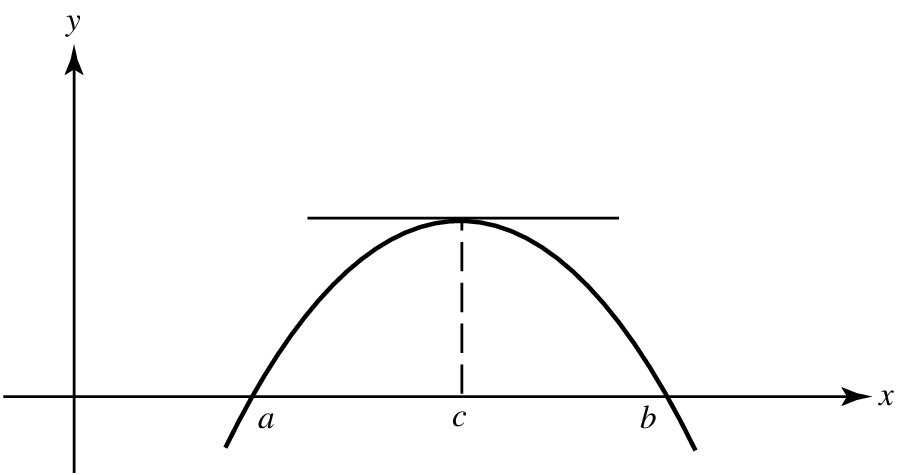
\includegraphics[width=3.05in,height=1.5in]{png/fig020304.png}
\end{center}
 \vskip6pt
 \refstepcounter{figure}
 \centerline{\bf Figure \thefigure} \label{figure:2.3.4}
 \vskip12pt

\begin{theorem}
[\href{http://www-history.mcs.st-and.ac.uk/Mathematicians/Rolle.html}
{Rolle}'s Theorem]
\label{thmtype:2.3.8}
Suppose that  $f$ is continuous on the closed interval $[a,b]$ and
differentiable on the open interval $(a,b),$ and $f(a)=f(b).$ Then
$f'(c)=0$ for some $c$ in the open interval $(a,b).$
\end{theorem}

\proof
Since $f$ is continuous on $[a,b]$, $f$ attains a maximum and a
minimum
value on $[a,b]$ (Theorem~\ref{thmtype:2.2.9}). If these two
extreme values are the same, then $f$ is constant on $(a,b)$, so
$f'(x)=0$ for all $x$ in $(a,b)$. If the extreme values differ, then
at least one must be attained at some point $c$ in the open interval
$(a,b)$, and $f'(c)=0$, by Theorem~\ref{thmtype:2.3.7}.
\bbox

\boxit{Intermediate Values of Derivatives}
A derivative may exist on an interval $[a,b]$ without being continuous
on $[a,b]$.  Nevertheless,  an intermediate value
theorem similar to Theorem~\ref{thmtype:2.2.10} applies to
derivatives.

\begin{theorem}[Intermediate Value Theorem for
Derivatives]\label{thmtype:2.3.9}
 Suppose that  $f$ is differentiable on $[a,b],$  $f'(a)\ne
f'(b),$ and $\mu$ is between $f'(a)$ and $f'(b).$ Then $f'(c)=\mu$
for some $c$ in $(a,b).$
\end{theorem}

\proof
 Suppose   first that
\begin{equation}\label{eq:2.3.17}
f'(a)<\mu<f'(b)
\end{equation}
and define
$$
g(x)=f(x)-\mu x.
$$
Then
\begin{equation}\label{eq:2.3.18}
g'(x)=f'(x)-\mu,\quad a\le x\le b,
\end{equation}
and \eqref{eq:2.3.17} implies that
\begin{equation}\label{eq:2.3.19}
g'(a)<0\mbox{\quad and\quad} g'(b)>0.
\end{equation}
Since $g$ is
continuous on $[a,b]$, $g$ attains a minimum at some point $c$ in
$[a,b]$. Lemma~\ref{thmtype:2.3.2} and \eqref{eq:2.3.19} imply that there is a
$\delta>0$ such that
$$
g(x)<g(a),\quad a<x<a+\delta,\mbox{\quad and\quad} g(x)<g(b),\quad
b-\delta<x<b
$$

\newpage
\noindent
(Exercise~\ref{exer:2.3.3}), and therefore $c\ne a$ and $c\ne b$. Hence,
$a<c<b$, and therefore $g'(c)=0$, by Theorem~\ref{thmtype:2.3.7}. From
\eqref{eq:2.3.18}, $f'(c)=\mu$.

 The proof for the case where
$f'(b)<\mu<f'(a)$
can be obtained by applying this result to  $-f$.
\bbox

\boxit{Mean Value Theorems}
\vspace*{-4ex}
\begin{theorem} [Generalized Mean Value Theorem]\label{thmtype:2.3.10}
If $f$ and $g$ are continuous on the closed interval $[a,b]$
and differentiable on the open interval $(a,b),$ then
\begin{equation} \label{eq:2.3.20}
[g(b)-g(a)]f'(c)=[f(b)-f(a)]g'(c)
\end{equation}
for some $c$ in $(a,b).$
\end{theorem}

\proof
The function
$$
h(x)=[g(b)-g(a)]f(x)-[f(b)-f(a)]g(x)
$$
is continuous on $[a,b]$ and differentiable on $(a,b)$, and
$$
h(a)=h(b)=g(b)f(a)-f(b)g(a).
$$
Therefore, Rolle's theorem implies that $h'(c)=0$ for some
$c$ in $(a,b)$. Since
$$
h'(c)=[g(b)-g(a)]f'(c)-[f(b)-f(a)]g'(c),
$$
this implies \eqref{eq:2.3.20}.
\bbox

The following special case of Theorem~\ref{thmtype:2.3.10} is important
enough to be
stated separately.

\begin{theorem} [Mean Value Theorem]\label{thmtype:2.3.11}
If $f$ is continuous on the closed interval $[a,b]$ and differentiable
on the open interval $(a,b),$ then
$$
f'(c)=\frac{f(b)-f(a)}{ b-a}
$$
for some $c$ in $(a,b).$
\end{theorem}

\proof Apply Theorem~\ref{thmtype:2.3.10} with $g(x)=x$.

\bbox

Theorem~\ref{thmtype:2.3.11} implies that the tangent to the curve
$y=f(x)$
at $(c,f(c))$ is parallel to the line connecting the points $(a,f(a))$
and $(b,f(b))$ on the curve (Figure~\ref{figure:2.3.5}, page
\pageref{figure:2.3.5}).

\boxit{Consequences of the Mean Value Theorem}
If $f$ is differentiable on $(a,b)$ and $x_1$, $x_2\in (a,b)$ then
$f$ is continuous on the closed interval with endpoints $x_1$ and
$x_2$ and differentiable on its interior. Hence, the mean value
theorem implies that
$$
f(x_2)-f(x_1)=f'(c)(x_2-x_1)
$$
for some $c$ between $x_1$ and $x_2$.  (This is true whether $x_1<x_2
$ or $x_2<x_1$.)  The next three theorems follow  from this.

\newpage
\begin{theorem}\label{thmtype:2.3.12}
If $f'(x)=0$ for all $x$ in $(a,b),$ then $f$ is constant on $(a,b).$
\end{theorem}

\begin{theorem}\label{thmtype:2.3.13}
If $f'$ exists and does not change sign on $(a,b),$ then $f$ is
monotonic on $(a,b):$ increasing$,$ nondecreasing$,$ decreasing$,$ or
nonincreasing as
$$
f'(x)>0,\quad f'(x)\ge0,\quad f'(x)<0,\mbox{\quad or\quad} f'(x)
\le0,
$$
respectively$,$ for all $x$ in $(a,b).$
\end{theorem}

\begin{theorem}\label{thmtype:2.3.14}
If
$$
|f'(x)|\le M,\quad a<x<b,
$$
then
\begin{equation} \label{eq:2.3.21}
|f(x)-f(x')|\le M |x-x'|,\quad x, x'\in (a,b).
\end{equation}
\end{theorem}

A function that satisfies an inequality like \eqref{eq:2.3.21} for all
$x$ and $x'$ in an interval is said to satisfy a
\href{http://www-history.mcs.st-and.ac.uk/Mathematicians/Lipschitz.html}
{\it Lipschitz}
{\it condition\/} on the interval.

 \vspace*{12pt}
\begin{center}
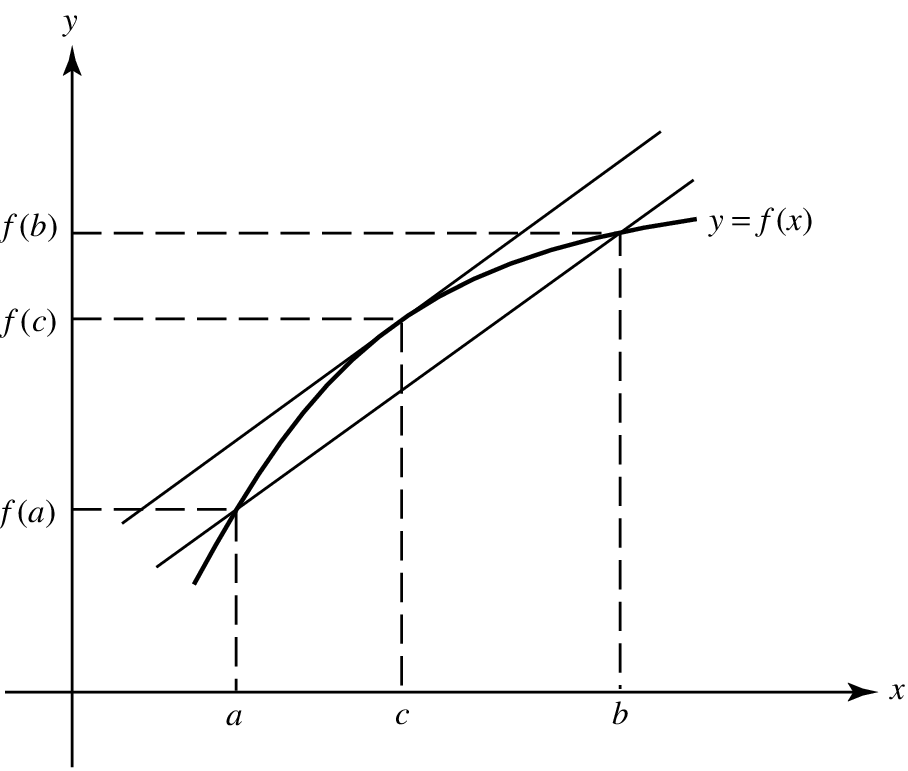
\includegraphics[width=3.1in,height=2.6in]{png/fig020305.png}
\end{center}
 \vskip6pt
 \refstepcounter{figure}
 \centerline{\bf Figure \thefigure} \label{figure:2.3.5}
 \vskip12pt

\exercises
\begin{exerciselist}

\item\label{exer:2.3.1}
 Prove that a function $f$ is differentiable at $x_0$ if and only if
$$
\lim_{x\to x_0}\frac{f(x)-f(x_0)-m(x-x_0)}{ x-x_0}=0
$$
for some constant $m$.  In this case, $f'(x_0)=m$.

\item\label{exer:2.3.2} Prove: If $f$ is defined on a neighborhood of
$x_0$, then $f$ is differentiable at $x_0$ if and only if the
discontinuity of
$$
h(x)=\frac{f(x)-f(x_0)}{ x-x_0}
$$
at $x_0$ is removable.

\item\label{exer:2.3.3} Use Lemma~\ref{thmtype:2.3.2} to prove that  if
$f'(x_0)>0$, there is a
$\delta>0$ such that
$$
f(x)<f(x_0) \mbox{\ if \ }  x_0-\delta<x<x_0
\mbox{\ and \ }
f(x)>f(x_0) \mbox{\ if \ }  x_0<x<x_0+\delta.
$$

\item\label{exer:2.3.4}
Suppose that  $p$ is continuous on $(a,c]$ and differentiable on $(a,c)$,
while $q$ is continuous on $[c,b)$ and differentiable on $(c,b)$.
 Let
$$
f(x)=\left\{\casespace\begin{array}{ll} p(x),&a<x\le c,\\[2\jot]
q(x),&c<x<b.\end{array}\right.
$$

\begin{alist}

\item % (a)
 Show that
$$
f'(x)=\left\{\casespace\begin{array}{ll} p'(x),&a<x<c,\\[2\jot]
q'(x),&c<x<b.\end{array}\right.
$$
\item % (b)
Under what additional conditions on $p$ and $q$ does
$f'(c)$ exist? Prove that your stated conditions are necessary and
sufficient.
\end{alist}

\item\label{exer:2.3.5}
Find all derivatives of $f(x)=x^{n-1}|x|$, where
$n$ is a positive integer.

\item\label{exer:2.3.6} Suppose that  $f'(0)$ exists and $f(x+y)=f(x)f(y)$
for all $x$ and $y$. Prove that $f'$ exists for all $x$.

\item\label{exer:2.3.7}
 Suppose that  $c'(0)=a$ and  $s'(0)=b$
where $a^2+b^2\ne0$, and
\begin{eqnarray*}
c(x+y)\ar=c(x)c(y)-s(x)s(y)\\
s(x+y)\ar=s(x)c(y)+c(x)s(y)
\end{eqnarray*}
for all $x$ and $y$.

\begin{alist}
\item % (a)
Show that $c$ and $s$ are differentiable on $(-\infty,\infty)$, and
find $c'$ and $s'$ in terms of $c$, $s$, $a$, and $b$.
\item % (b)
 (For those who have studied differential equations.)  Find
$c$ and $s$ explicitly.
\end{alist}

\item\label{exer:2.3.8}
\begin{alist}
\item % (a)
Suppose that  $f$ and $g$ are differentiable at $x_0$,
$f(x_0)=g(x_0)=0$, and $g'(x_0)\ne0$.  Without using L'Hospital's
rule, show that
$$
\lim_{x\to x_0}\frac{f(x)}{ g(x)}=\frac{f'(x_0)}{ g'(x_0)}.
$$
\item % (b)
 State the corresponding results for one-sided limits.
\end{alist}
\item\label{exer:2.3.9} Prove Theorem~\ref{thmtype:2.3.4}\part{a}.

\item\label{exer:2.3.10} Prove Theorem~\ref{thmtype:2.3.4}\part{b}.

\item\label{exer:2.3.11} Prove Theorem~\ref{thmtype:2.3.4}\part{d}.

\item\label{exer:2.3.12}
Prove by induction:  If $n\ge1$ and  $f^{(n)}(x_0)$ and $g^{(n)}(x_0)$
exist, then so does
$(fg)^{(n)}(x_0)$, and
$$
(fg)^{(n)}(x_0)=
\sum_{m=0}^n{\binom n m}f^{(m)}(x_0)g^{(n-m)}(x_0).
$$
\hint{See Exercise~$\ref{exer:1.2.19}.$} This is
\href{http://www-history.mcs.st-and.ac.uk/Mathematicians/Leibniz.html}
{\it Leibniz}{\it's rule\/}
 for differentiating a product.

\item\label{exer:2.3.13} What is wrong with the ``proof'' of the chain
rule suggested after Example~\ref{example:2.3.3}? Correct it.

\item\label{exer:2.3.14}
Suppose that  $f$ is continuous and increasing on
$[a,b]$. Let $f$ be differentiable at a point $x_0$ in $(a,b)$, with
$f'(x_0) \ne0$. If $g$ is the inverse of $f$
Theorem~\ref{thmtype:2.2.15}), show that $g'(f(x_0))=1/f'(x_0)$.

\item\label{exer:2.3.15}
\begin{alist}
\item % (a)
  Show that $f_+'(a)=f'(a+)$ if both quantities exist.
\item % (b)
Example~\ref{example:2.3.4} shows that $f_+'(a)$ may exist even if
$f'(a+)$ does not. Give an example where $f'(a+)$ exists but
$f_+'(a)$ does not.
\item % (c)
Complete the following statement so  it becomes a theorem, and
prove the theorem: ``If $f'(a+)$ exists and $f$ is
\mbox{}\hrulefill\mbox{} at $a$, then $f_+'(a)=f'(a+)$.''
\end{alist}

\item\label{exer:2.3.16} Show that $f(a+)$ and $f(b-)$ exist (finite) if
$f'$ is bounded on $(a,b)$.
\hint{See Exercise~$\ref{exer:2.1.38}.$}

\item\label{exer:2.3.17} Suppose that  $f$ is continuous on $[a,b]$,
$f_+'(a)$ exists, and $\mu$ is between $f_+'(a)$ and
$(f(b)-f(a))/(b-a)$. Show that $f(c)-f(a)=\mu (c-a)$ for
some $c$ in $(a,b)$.

\item\label{exer:2.3.18}
Suppose that  $f$ is continuous on $[a,b]$, $f_+'(a)<\mu<f_-'(b)$, and
$$
(f(b)-f(a))/(b-a)\ne\mu.
$$
 Show that either $f(c)-f(a)=\mu(c-a)$ or
$f(c)-f(b)=\mu(c-b)$ for some $c$ in $(a,b)$.

\item\label{exer:2.3.19}
Let
$$
f(x)=\frac{\sin x}{ x},\quad x\ne0.
$$
\begin{alist}
\item % (a)
 Define $f(0)$ so that $f$ is continuous at $x=0$.
\hint{Use Exercise~$\ref{exer:2.3.8}.$}
\item % (b)
Show that if $\overline{x}$ is a local extreme point of $f$,
then
$$
|f(\overline{x})|=(1+\overline{x}^2)^{-1/2}.
$$
\hint{Express $\sin x$ and $\cos x$ in terms of $f(x)$ and $f'(x),$
and add their squares to obtain a useful identity$.$}

\item % (c)
 Show that $|f(x)|\le1$ for all $x$.  For what
value of $x$ is equality attained?
\end{alist}

\newpage

\item\label{exer:2.3.20} Let $n$ be a positive
integer and
$$
f(x)=\frac{\sin nx}{ n\sin x},\quad x\ne k\pi \mbox{\quad
($k=$ integer)}.
$$

\begin{alist}
\vspace*{1pt}
\item % (a)
Define $f(k\pi)$ so that $f$ is continuous at $k\pi$.
\hint{Use Exercise~$\ref{exer:2.3.8}.$}
\vspace*{1pt}
\item % (b)
 Show that if $\overline{x}$ is a local extreme point of $f$,
 then
$$
|f(\overline{x})|=
\left[1+(n^2-1)\sin^2\overline{x}\right]^{-1/2}.
$$
\hint{Express $\sin nx$ and $\cos nx$ in terms of $f(x)$ and
$f'(x),$ and add their squares to obtain a useful identity$.$}
\vspace*{1pt}
\item % (c)
\vspace*{1pt}
Show that $|f(x)|\le1$ for all $x$.  For what
values of $x$ is equality attained?
\end{alist}
\vspace*{1pt}

\item\label{exer:2.3.21} We say that $f$ has at least $n$ zeros, {\it
counting multiplicities\/},
 on an interval
$I$ if
there are distinct points $x_1$, $x_2$, \dots, $x_p$ in $I$ such that
$$
f^{(j)}(x_i)=0,\quad 0\le j\le n_i-1,\quad 1\le i\le p,
$$
and $n_1+\cdots+n_p=n$.
Prove: If $f$ is differentiable and has at least $n$ zeros, counting
multiplicities, on an interval $I$, then $f'$ has at least $n-1$
zeros, counting multiplicities, on $I$.
\vspace*{1pt}

\item\label{exer:2.3.22} Give an example of a function $f$ such that $f'$
exists on an interval $(a,b)$ and has a jump discontinuity at a point
$x_0$ in $(a,b)$, or show that there is no such function.
\vspace*{1pt}

\item\label{exer:2.3.23} Let $x_1$, $x_2$, \dots, $x_n$ and
$y_1$, $y_2$, \dots, $y_n$ be in
$(a,b)$ and $y_i<x_i$, $1\le i\le n$. Show that if $f$ is
differentiable on $(a,b)$, then
$$
\sum_{i=1}^n\,[f(x_i)-f(y_i)]=f'(c)\sum_{i=1}^n\, (x_i-y_i)
$$
for some $c$ in $(a,b)$.
\vspace*{1pt}

\item\label{exer:2.3.24} Prove or give a counterexample: If $f$ is
differentiable on a neighborhood of $x_0$, then $f$ satisfies a
Lipschitz condition on some neighborhood of $x_0$.

\vspace*{1pt}

\item\label{exer:2.3.25}  Let
$$
f''(x)+p(x) f(x)=0\mbox{\quad and \quad} g''(x)+p(x)g(x)=0,\quad
a<x<b.
$$
\begin{alist}
\vspace*{1pt}
\item % (a)
 Show that  $W=f'g-fg'$ is constant on $(a,b)$.
\vspace*{1pt}
\item % (b)
 Prove:  If $W\ne0$ and $f(x_1)=f(x_2)=0$ where
$a<x_1<x_2<b$, then $g(c)=0$ for some $c$ in $(x_1,x_2)$. \hint{
Consider $f/g.$}
\end{alist}

\newpage

\item\label{exer:2.3.26} Suppose that  we extend the definition of
differentiability by saying that $f$ is differentiable at $x_0$ if
$$
f'(x_0)=\lim_{x\to x_0}\frac{f(x)-f(x_0)}{ x-x_0}
$$
exists in the extended reals.  Show that if
$$
f(x)=\left\{\casespace\begin{array}{ll}\sqrt{x}, & x\ge0,\\[2\jot]
-\sqrt{-x},&x<0,\end{array}\right.
$$
then $f'(0)=\infty$.

\item\label{exer:2.3.27} Prove or give a counterexample: If $f$ is
differentiable at $x_0$ in the extended sense of
Exercise~\ref{exer:2.3.26}, then $f$ is continuous at $x_0$.

\item\label{exer:2.3.28}
Assume that $f$ is differentiable on $(-\infty,\infty)$
and $x_0$ is a critical point of $f$.

\begin{alist}
\item % (a)
Let $h(x)=f(x)g(x)$, where $g$ is differentiable on $(-\infty,\infty)$
and
$$
f(x_0)g'(x_0)\ne0.
$$
 Show that the tangent line to the curve
$y=h(x)$ at $(x_0,h(x_0))$ and the tangent line to the curve $y=g(x)$
at $(x_0,g(x_0)$ intersect on the $x$-axis.

\item % (b)
Suppose that  $f(x_0)\ne0$. Let $h(x)=f(x)(x-x_1)$, where $x_1$ is
arbitrary.
Show that the tangent line to the curve $y=h(x)$ at $(x_0,h(x_0))$
intersects the $x$-axis at $\overline x=x_1$.

\item % (c)
Suppose that  $f(x_0)\ne0$. Let $h(x)=f(x)(x-x_1)^2$, where $x_1\ne
x_0$.
Show that the tangent line to the curve $y=h(x)$ at $(x_0,h(x_0))$
intersects the $x$-axis at the midpoint of the interval with endpoints
$x_0$ and $x_1$.

\item % (d)
Let $h(x)=(ax^2+bx+c)(x-x_1)$, where $a\ne0$ and $b^2-4ac\ne0$. Let
$x_0=-\dst\frac{b}{2a}$. Show that the tangent line to the curve
$y=h(x)$ at   $(x_0,h(x_0))$ intersects the $x$-axis at $\overline
x=x_1$.

\item % (e)
Let $h$ be a cubic polynomial with zeros $\alpha$, $\beta$, and
$\gamma$, where $\alpha$ and $\beta$ are distinct and $\gamma$ is
real. Let $x_0=\dst\frac{\alpha+\beta}{2}$. Show that the tangent
line to the curve $y=h(x)$ at $(x_0,h(x_0))$ intersects the axis at
$\overline x=\gamma$.
\end{alist}
\label{sectionend:\thesection}
\end{exerciselist}


\currentpdfbookmark{Section 2.4 L'Hospital's Rule}{section:2.4}
\newsection{4}{Differential Calculus of Functions of One Variable
}{L'Hospital's Rule}

\renewcommand{\thissection}{\sectiontitle{L'HOSPITAL'S RULE}}

\thissection


\noindent
The method of Theorem~\ref{thmtype:2.1.4} for finding limits
of the sum, difference,
product, and quotient of functions breaks down in connection
with indeterminate forms. The generalized mean value theorem
(Theorem~\ref{thmtype:2.3.10})  leads to
 a method for evaluating limits of indeterminate forms.

\begin{theorem}
[\href{http://www-history.mcs.st-and.ac.uk/Mathematicians/De_L'Hopital.html}
{L'Hospital}'s Rule]
\label{thmtype:2.4.1}
Suppose that $f$ and $g$ are differentiable and $g'$ has no zeros on
$(a,b).$ Let
\begin{equation}\label{eq:2.4.1}
\lim_{x\to b-}f(x)=\lim_{x\to b-}g(x)=0
\end{equation}

\newpage

\noindent
or
\begin{equation}\label{eq:2.4.2}
\lim_{x\to b-}f(x)=\pm\infty\mbox{\quad and \quad} \lim_{x\to
b-}g(x)=\pm\infty,
\end{equation}
and suppose that
\begin{equation}\label{eq:2.4.3}
\lim_{x\to b-}\frac{f'(x)}{ g'(x)}=L\quad\mbox{$($finite or $\pm
\infty)$}.
\end{equation}
Then
\begin{equation}\label{eq:2.4.4}
\lim_{x\to b-}\frac{f(x)}{ g(x)}=L.
\end{equation}
\end{theorem}

\proof
 We prove the theorem for finite $L$ and leave the case where
$L=\pm\infty$ to you (Exercise~\ref{exer:2.4.1}).

\enlargethispage{100pt}
 Suppose that
$\epsilon >0$. From \eqref{eq:2.4.3}, there is an $x_0$ in $(a,b)$ such
that
\begin{equation}\label{eq:2.4.5}
\left|\frac{f'(c)}{g'(c)}-L\right|<\epsilon\mbox{\quad if\quad}
x_0
<c<b.
\end{equation}
Theorem~\ref{thmtype:2.3.10} implies that if $x$ and $t$ are in $[x_0,
b)$, then there is a $c$ between them, and therefore in
$(x_0,b)$, such that
\begin{equation}\label{eq:2.4.6}
[g(x)-g(t)]f'(c)=[f(x)-f(t)]g'(c).
\end{equation}
Since $g'$ has no zeros in $(a,b)$, Theorem~\ref{thmtype:2.3.11}
implies that
$$
g(x)-g(t)\ne0\mbox{\quad if\quad} x, t\in (a,b).
$$
This means that $g$ cannot have more than one zero in $(a,b)$.
Therefore,
we can choose $x_0$ so that, in addition to \eqref{eq:2.4.5}, $g$ has
no zeros in $[x_0,b)$. Then \eqref{eq:2.4.6} can be
rewritten as
$$
\frac{f(x)-f(t)}{ g(x)-g(t)}=\frac{f'(c)}{ g'(c)},
$$
so \eqref{eq:2.4.5} implies that
\begin{equation}\label{eq:2.4.7}
\left|\frac{f(x)-f(t)}{ g(x)-g(t)}-L\right|<\epsilon \mbox{\quad if\quad}
x, t\in [x_0,b).
\end{equation}

If \eqref{eq:2.4.1} holds, let $x$ be fixed in $[x_0,b)$, and consider
the function
$$
G(t)=\frac{f(x)-f(t)}{ g(x)-g(t)}-L.
$$
From \eqref{eq:2.4.1},
$$
\lim_{t\to b-}f(t)=\lim_{t\to b-}g(t)=0,
$$
so
\begin{equation}\label{eq:2.4.8}
\lim_{t\to b-}G(t)=\frac{f(x)}{g(x)}-L.
\end{equation}

\newpage
\noindent
Since
$$
|G(t)|<\epsilon\mbox{\quad if\quad} x_0<t<b,
$$
because of \eqref{eq:2.4.7}, \eqref{eq:2.4.8} implies that
$$
\left|\frac{f(x)}{ g(x)}-L\right|\le\epsilon.
$$
This holds for all $x$ in $(x_0,b)$, which implies \eqref{eq:2.4.4}.

The proof under assumption \eqref{eq:2.4.2} is more complicated. Again
choose $x_0$ so that \eqref{eq:2.4.5} holds and $g$  has no zeros
in
$[x_0,b)$. Letting $t=x_0$ in
\eqref{eq:2.4.7}, we see that
\begin{equation} \label{eq:2.4.9}
\left|\frac{f(x)-f(x_0)}{ g(x)-g(x_0)}-L\right|<\epsilon \mbox{\quad
if\quad} x_0\le x<b.
\end{equation}
Since  $\lim_{x\to b-}f(x)=\pm\infty$, we can choose $x_1>x_0$
so that $f(x)\ne0$ and $f(x)\ne f(x_0)$ if $x_1<x<b$. Then
the function
$$
u(x)=\frac{1-g(x_0)/g(x)}{1-f(x_0)/f(x)}
$$
is defined and nonzero if $x_1<x<b$, and
\begin{equation}\label{eq:2.4.10}
\lim_{x\to b-} u(x)=1,
\end{equation}
because of \eqref{eq:2.4.2}.

Since
$$
\frac{f(x)-f(x_0)}{ g(x)-g(x_0)}=\frac{f(x)}{ g(x)}\
\frac{1-f(x_0)/f(x)}{
1-g(x_0)/g(x)}=\frac{f(x)}{ g(x)u(x)},
$$
\eqref{eq:2.4.9} implies that
$$
\left|\frac{f(x)}{ g(x) u(x)}-L\right|<\epsilon\mbox{\quad if\quad}
x_1<x<b,
$$
which can be rewritten as
\begin{equation} \label{eq:2.4.11}
\left|\frac{f(x)}{ g(x)}-Lu(x)\right|<\epsilon |u(x)|\mbox{\quad if
\quad}x_1<x<b.
\end{equation}
From this and the triangle inequality,
\begin{equation}\label{eq:2.4.12}
\left|\frac{f(x)}{ g(x)}-L\right|\le\left|\frac{f(x)}{ g(x)}-Lu(x)\right|
+|Lu(x)-L|\le\epsilon|u(x)|+|L|\,|u(x)-1|.
\end{equation}
Because of \eqref{eq:2.4.10}, there is a point $x_2$ in $(x_1,b)$ such
that
$$
|u(x)-1|<\epsilon\mbox{\quad and therefore \quad} |u(x)|<1+\epsilon
\mbox{\quad if\quad} x_2<x<b.
$$
This, \eqref{eq:2.4.11}, and \eqref{eq:2.4.12} imply that
$$
\left|\frac{f(x)}{ g(x)}-L\right|<\epsilon (1+\epsilon)+|L|\epsilon
\mbox{\quad if\quad} x_2<x<b,
$$

\newpage
\noindent
which proves \eqref{eq:2.4.4} under assumption \eqref{eq:2.4.2}.
\bbox

Theorem~\ref{thmtype:2.4.1} and the proof given here remain valid if
$b=\infty$ and ``$x\to b-$'' is replaced by ``$x\to\infty$''
throughout. Only minor changes in the proof are required to show that
similar theorems are valid for limits from the right, limits at
$-\infty$, and ordinary (two-sided) limits. We will take these as
given.

\boxit{The Indeterminate Forms $\mathbf{0/0}$ and
$\mathbf{\mathbf{\infty}/\mathbf{\infty}}$}
\hskip-.4em
We say that $f/g$ {\it is  of the  form $0/0$ as\/}
$x\to b-$ if
$$
\lim_{x\to b-}f(x)=\lim_{x\to b-}g(x)=0,
$$
or {\it  of the  form $\infty/\infty$ as $x\to b-$\/} if
$$
\lim_{x\to b-} f(x)=\pm\infty
$$
and
$$
\lim_{x\to b-}
g(x)=\pm\infty.
$$
The corresponding definitions for $x\to b+$ and $x\to\pm\infty$ are
similar.  If $f/g$ is of one of these forms as $x\to b-$ and as $x\to
b+$, then we say that it is of that form as $x\to b$.

\begin{example}\label{example:2.4.1}\rm   The ratio $\sin x/x$ is of the
form $0/0$ as $x\to 0$, and L'Hospital's rule yields
$$
\lim_{x\to 0}\frac{\sin x}{ x}=\lim_{x\to 0}\frac{\cos x}{1}=1.
$$
\end{example}

\begin{example}\label{example:2.4.2}\rm   The ratio $e^{-x}/x$ is of the
form $\infty/\infty$ as $x\to-\infty$, and L'Hospital's rule yields
$$
\lim_{x\to-\infty}\frac{e^{-x}}{ x}=\lim_{x\to-\infty}\frac
{-e^{-x}}{1}=-\infty.
$$
\end{example}

\begin{example}\label{example:2.4.3}\rm   Using L'Hospital's rule may lead to
another indeterminate form; thus,
$$
\lim_{x\to\infty}\frac{e^x}{ x^2}=\lim_{x\to\infty}\frac{e^x}{2x}
$$
if the limit on the right exists in the extended reals.  Applying
L'Hospital's rule again yields
$$
\lim_{x\to\infty}\frac{e^x}{2x}=\lim_{x\to\infty}\frac{e^x}{2}=
\infty.
$$
Therefore,
$$
\lim_{x\to\infty}\frac{e^x}{ x^2}=\infty.
$$
More generally,
$$
\lim_{x\to\infty}\frac{e^x}{ x^\alpha}=\infty
$$
for any real number $\alpha$ (Exercise~\ref{exer:2.4.33}).
\end{example}

\begin{example}\label{example:2.4.4}\rm   Sometimes it pays to combine
L'Hospital's rule with other manipulations.  For example,
\begin{eqnarray*}
\lim_{x\to0}\frac{4-4\cos x-2\sin^2 x}{ x^4}\ar=\lim_{x\to 0}
\frac{4\sin x-4\sin x\cos x}{4x^3}\\
\ar=\left(\lim_{x\to 0}\frac{\sin x}{ x}\right)\left(\lim_{x\to 0}
\frac{1-\cos x}{ x^2}\right)\\
\ar=\left(\lim_{x\to 0}\frac{\sin x}{ x}\right)\left(\lim_{x\to 0}
\frac{\sin x}{2x}\right)\\
\ar=\frac{1}{2}\left(\lim_{x\to 0}\frac{\sin x}{ x}\right)^2\\
\ar=\frac{1}{2}(1)^2=\frac{1}{2} \mbox{\quad
(Example~\ref{example:2.4.1})}.
\end{eqnarray*}

As another example, L'Hospital's rule yields
$$
\lim_{x\to0}\frac{e^{-x^2}\log (1+x)}{ x}=\lim_{x\to0}
\frac{-2xe^{-x^2}\log (1+x)+e^{-x^2}(1+x)^{-1}}{1}=1.
$$
However, it is better to remove the ``determinate'' part of the ratio
before using L'Hospital's rule:
\begin{eqnarray*}
\lim_{x\to 0}\frac{e^{-x^2}\log (1+x)}{ x}\ar=\left(\lim_{x\to 0}
e^{-x^2}\right)
\left(\lim_{x\to 0}\frac{\log (1+x)}{ x}\right)\\
\ar=(1)\lim_{x\to 0}\frac{\log (1+x)}{ x}
\end{eqnarray*}
$$
\hspace*{.52in}=\lim_{x\to 0}\frac{1/(1+x)}{1}=1.
\eqno{\bbox}
$$
\end{example}

In using L'Hospital's rule we usually write, for example,
\begin{equation}\label{eq:2.4.13}
\lim_{x\to b}\frac{f(x)}{ g(x)}=\lim_{x\to b}\frac{f'(x)}{ g'(x)}
\end{equation}
and then try to find the limit on the right. This is convenient, but
technically incorrect, since \eqref{eq:2.4.13} is true only if the limit
on the
right exists in the extended reals. It may happen that the limit on
the left exists but the one on the right does not. In this case,
\eqref{eq:2.4.13} is  incorrect.

\begin{example}\label{example:2.4.5}\rm   If
$$
f(x)=x-x^2\sin \frac{1}{ x}\mbox{\quad and\quad} g(x)=\sin x,
$$
then
$$
f'(x)=1-2x\sin \frac{1}{ x}+\cos \frac{1}{ x}\mbox{\quad and\quad}
g'(x)=\cos x.
$$

\newpage
\noindent
Therefore, $\lim_{x\to 0} f'(x)/g'(x)$ does not exist. However,
$$
\lim_{x\to 0}\frac{f(x)}{ g(x)}=\lim_{x\to 0}\frac{1-x\sin(1/x)}{
(\sin x)/x}=\frac{1}{1}=1.
$$
\end{example}

\boxit{The Indeterminate Form $\mathbf{0\cdot\mathbf{\infty}}$}
We say that a product $fg$  {\it is  of the form
$0\cdot
\infty$ as $x\to b-$\/} if one of the factors approaches $0$ and the
other approaches $\pm\infty$ as $x\to b-$. In this case, it may be
useful to apply L'Hospital's rule after writing
$$
f(x)g(x)=\frac{f(x)}{1/g(x)}\mbox{\quad or\quad}
f(x)g(x)=\frac{g(x)}{1/f(x)},
$$
since one of these ratios is of the form $0/0$ and the other is of the
form $\infty/\infty$ as $x\to b-$.

Similar statements apply to limits as $x\to b+$, $x\to b$, and $x\to
\pm\infty$.

\begin{example}\label{example:2.4.6}\rm
The product $x\log x$ is of the form $0\cdot\infty$ as $x\to0+$.
Converting it to an $\infty/\infty$ form yields
\begin{eqnarray*}
\lim_{x\to 0+} x\log x\ar=\lim_{x\to 0+}\frac{\log x}{1/x}\\[2\jot]
\ar=\lim_{x\to 0+}\frac{1/x}{-1/x^2}\\[2\jot]
\ar=-\lim_{x\to 0+} x=0.
\end{eqnarray*}
Converting  to a $0/0$ form leads to a more complicated problem:
\begin{eqnarray*}
\lim_{x\to 0+} x\log x\ar=\lim_{x\to 0+}\frac{x}{1/\log x}\\[2\jot]
\ar=\lim_{x\to 0+}\frac{1}{-1/x(\log x)^2}\\[2\jot]
\ar=-\lim_{x\to0+} x(\log x)^2=\, ?
\end{eqnarray*}
\end{example}


        \enlargethispage{100pt}

\begin{example}\label{example:2.4.7}\rm
The product $\dst x\log(1+1/x)$ is of the form $0\cdot\infty$
as $x\to\infty$. Converting it to a $0/0$ form yields
\begin{eqnarray*}
\lim_{x\to\infty} x\log (1+1/x)\ar=\lim_{x\to\infty}\frac {\log
(1+1/x)}{
1/x}\\[2\jot]
\ar=\lim_{x\to\infty} \frac{\left[1/(1+1/x)\right]
(-1/x^2)}{-1/x^2}\\[2\jot]
\ar=\lim_{x\to\infty}\frac{1}{1+1/x}=1.
\end{eqnarray*}

\newpage
\noindent
  In this
case, converting to an $\infty/\infty$ form complicates the problem:
\begin{eqnarray*}
\lim_{x\to\infty}
x\log(1+1/x)\ar=\lim_{x\to\infty}\frac{x}{1/\log(1+1/x)}
\\
\ar=\lim_{x\to\infty}
\frac{1}{\dst\left(\frac{-1}{[\log(1+1/x)]^2}\right)
\left(\frac{-1/x^2}{1+1/x}\right)}\\
\ar=\lim_{x\to\infty}x(x+1)[\log(1+1/x)]^2=\, ?
\end{eqnarray*}
\end{example}


\boxit{The Indeterminate Form
$\mathbf{\mathbf{\infty}-\mathbf{\infty}}$}
A difference $f-g$  {\it is of the form
$\infty-\infty$ as $x\to b-$\/} if
$$
\lim_{x\to b-} f(x)=\lim_{x\to b-} g(x)=\pm\infty.
$$
In this case, it may be possible to manipulate $f-g$ into an
expression that is no longer indeterminate, or is of the form $0/0$ or
$\infty/\infty$ as $x\to b-$. Similar remarks apply to limits as $x\to
b+$, $x\to b$, or $x\to\pm\infty$.

\begin{example}\label{example:2.4.8}\rm   The difference
$$
\frac{\sin x}{ x^2}-\frac{1}{ x}
$$
is of the form $\infty-\infty$ as $x\to 0$, but it can be rewritten as
the $0/0$ form
$$
\frac{\sin x-x}{ x^2}.
$$
Hence,
\begin{eqnarray*}
\lim_{x\to 0}\left(\frac{\sin x}{x^2}-\frac{1}{
x}\right)\ar=\lim_{x\to
0} \frac{\sin x-x}{ x^2}=\lim_{x\to 0}\frac{\cos x-1}{2x}\\
\ar=\lim_{x\to 0}\frac{-\sin x}{2}=0.
\end{eqnarray*}
\end{example}

\enlargethispage{100pt}

\begin{example}\label{example:2.4.9}\rm   The difference
$$
x^2-x
$$
is of the form $\infty-\infty$ as $x\to\infty$.  Rewriting it as
$$
x^2\left(1-\frac{1}{ x}\right),
$$
which is no longer indeterminate as $x\to\infty$, we find that
\begin{eqnarray*}
\lim_{x\to\infty}(x^2-x)\ar=\lim_{x\to\infty}x^2\left(1-\frac{1}{
x}\right)\\
\ar=\left(\lim_{x\to\infty}x^2\right)\lim_{x\to\infty}\left(1-\frac{1}{
x}\right)
\\ \ar =(\infty)(1)=\infty
\end{eqnarray*}
\end{example}

\newpage

\boxit{The Indeterminate Forms $\mathbf{0^0}$,
$\mathbf{1^{\mathbf{\infty}}}$, and
$\mathbf{\mathbf{\infty}^0}$}
The function $f^g$ is defined by
$$
f(x)^{g(x)}=e^{g(x)\log f(x)}=\exp(g(x)\log f(x))
$$
for all $x$ such that $f(x)>0$.  Therefore, if $f$ and $g$ are defined
and $f(x)>0$ on an interval $(a,b)$, Exercise~\ref{exer:2.2.22}
implies that
\begin{equation}\label{eq:2.4.14}
\lim_{x\to b-}[f(x)]^{g(x)}=\exp\left(\lim_{x\to b-}
g(x)\log f(x)\right)
\end{equation}
if $\lim_{x\to b-}g(x)\log f(x)$ exists in the extended reals.  (If
this limit is $\pm\infty$ then  \eqref{eq:2.4.14} is valid if we define
$e^{-\infty}=0$ and $e^\infty=\infty$.) The product $g\log f$ can be
 of the form $0\cdot\infty$ in three ways as $x\to b-$:
\vskip10pt

\begin{alist}
\item % (a)
 If $\lim_{x\to b-} g(x)=0$ and $\lim_{x\to b-}f(x)=0$.
\item % (b)
 If $\lim_{x\to b-}g(x)=\pm\infty$ and $\lim_{x\to
b-}f(x)=1$.
\item % (c)
 If $\lim_{x\to b-}g(x)=0$ and $\lim_{x\to b-}f(x)=
\infty$.
\end{alist}
\vskip10pt
In these three cases, we say that $f^g$  {\it is
of the form $0^0$, $1^\infty$, and $\infty^0$, respectively, as $x\to
b-$\/}.
Similar definitions apply to limits as $x\to b+$, $x\to b$, and
$x\to\pm\infty$.

\vskip10pt
\begin{example}\label{example:2.4.10}\rm The function $x^x$ is of the
form $0^0$ as $x\to 0+$. Since
$$
x^x=e^{x\log x}
$$
and $\lim_{x\to 0+} x\log x=0$ (Example~\ref{example:2.4.6}),
$$
\lim_{x\to 0+} x^x=e^0=1.
$$
\end{example}

\vskip10pt

\begin{example}\label{example:2.4.11}\rm   The function
$x^{1/(x-1)}$
is of the form $1^\infty$ as $x\to 1$.  Since
\begin{eqnarray*}
x^{1/(x-1)}=\exp\left(\frac{\log x}{x-1}\right)\\
\arraytext{and}\\
\lim_{x\to1}\frac{\log x}{ x-1}=\lim_{x\to 1}\frac{1/x}{1}=1,
\end{eqnarray*}
it follows that
$$
\lim_{x\to 1} x^{1/(x-1)}=e^1=e.
$$
\end{example}

\enlargethispage{100pt}
\begin{example}\label{example:2.4.12}\rm   The function $x^{1/x}$ is of the
form $\infty^0$ as $x\to\infty$.  Since
\begin{eqnarray*}
x^{1/x}\ar=\exp\left(\frac{\log x}{ x}\right)\\
\arraytext{and}\\
\lim_{x\to\infty}\frac{\log x}{ x}\ar=\lim_{x\to\infty}\frac{1/x}{1}
=0,\\
\end{eqnarray*}

\newpage
\noindent
it follows that
$$
\lim_{x\to\infty} x^{1/x}=e^0=1.
$$
\end{example}
\exercises
\begin{exerciselist}
\item\label{exer:2.4.1}
Prove Theorem~\ref{thmtype:2.4.1} for the case where $\lim_{x\to
b-}f'(x)/g'(x)=\pm\infty$.

\exercisetext{In
 Exercises~$\ref{exer:2.4.2}$--$\ref{exer:2.4.40}$,
 find the indicated limits.}
\threetab

\vspace*{-4pt}\item\label{exer:2.4.2} $\dst\lim_{x\to
0}\frac{\tan^{-1}x}{\sin^{-1}x}$ &
\item\label{exer:2.4.3} $\dst\lim_{x\to 0}\frac{1-\cos
x}{\log(1+x^2)}$&
\vspace{1.2ex}
\vspace*{-4pt}\item\label{exer:2.4.4} $\dst\lim_{x\to 0+}\frac{1+\cos
x}{e^x-1}$\\
\end{tabular}

\threetab
\item\label{exer:2.4.5} $\dst\lim_{x\to\pi}\frac{\sin nx}{\sin x}$&
\item\label{exer:2.4.6} $\dst\lim_{x\to 0}\frac{\log(1+x)}{
x}$&
 \item\label{exer:2.4.7} $\dst\lim_{x\to\infty}e^x\sin e^{-x^2}$\\
\end{tabular}

\threetab
\item\label{exer:2.4.8} $\dst\lim_{x\to\infty} x\sin(1/x)$&
\vspace*{-3pt}\item\label{exer:2.4.9}
$\dst\lim_{x\to\infty}\sqrt{x}(e^{-1/x}-1)$&
\item\label{exer:2.4.10} $\dst\lim_{x\to 0+}\tan x\log x$
\end{tabular}

\twotab
\item\label{exer:2.4.11} $\dst\lim_{x\to\pi}\sin x\log (|\tan x|)$&
\vspace*{-8pt}\item\label{exer:2.4.12} $\dst\lim_{x\to 0+}
{\left[\frac{1}{x}+\log(\tan x)\right]}$\\
\end{tabular}

\twotab
\item\label{exer:2.4.13} $\dst\lim_{x\to\infty} (\sqrt{x+1}-\sqrt{x})$&
\vspace*{-8pt}\item\label{exer:2.4.14} $\dst\lim_{x\to 0}
\left(\frac{1}{ e^x-1}-\frac{1}{ x}\right)$\\
\end{tabular}

\twotab
\item\label{exer:2.4.15} $\dst\lim_{x\to 0} (\cot x-\csc x)$&
\vspace*{-8pt}\item\label{exer:2.4.16} $\dst\lim_{x\to 0}
{\left(\frac{1}{\sin x}-\frac{1}{ x}\right)}$\\
\end{tabular}

\twotab
\item\label{exer:2.4.17} $\dst\lim_{x\to\pi} |\sin x|^{\tan x}$&
\item\label{exer:2.4.18} $\dst\lim_{x\to\pi/2} |\tan x|^{\cos x}$\\
\end{tabular}

\twotab
\item\label{exer:2.4.19} $\dst\lim_{x\to 0} |\sin x|^x$&
\vspace*{-3pt}\item\label{exer:2.4.20} $\dst\lim_{x\to 0}(1+x)^{1/x}$\\
\end{tabular}

\twotab
\item\label{exer:2.4.21} $\dst\lim_{x\to\infty} x^{\sin(1/x)}$&
\vspace*{-8pt}\item\label{exer:2.4.22} $\dst\lim_{x\to 0}
{\left(\frac{x}{1-\cos x}-\frac{2}{ x}\right)}$\\
\end{tabular}

\twotab
\item\label{exer:2.4.23} $\dst\lim_{x\to 0+} x^\alpha\log x$&
\vspace*{-8pt}\item\label{exer:2.4.24} $\dst\lim_{x\to e}
\frac{\log(\log x)}{\sin(x-e)}$\\
\end{tabular}

\twotab

\item\label{exer:2.4.25} $\dst\lim_{x\to\infty}{\left(\frac{x+1}{
x-1}\right)}^{\sqrt{x^2-1}}$&
\item\label{exer:2.4.26} $\dst\lim_{x\to 1+}{\left(
\frac{x+1}{ x-1}\right)}^{\sqrt{x^2-1}}$\\
\end{tabular}

\twotab
\item\label{exer:2.4.27} $\dst\lim_{x\to\infty}\frac{(\log x)^\beta}{ x}$&
\vspace*{8pt}\item\label{exer:2.4.28}$\dst\lim_{x\to\infty}(\cosh x-\sinh x)$\\
\end{tabular}

\twotab
\item\label{exer:2.4.29} $\dst\lim_{x\to\infty}(x^\alpha-\log x)$&
\vspace*{-8pt}\item\label{exer:2.4.30}
$\dst\lim_{x\to-\infty}e^{x^2}\sin(e^x)$\\
\end{tabular}

\newpage

\twotab
\item\label{exer:2.4.31} $\dst\lim_{x\to\infty} x(x+1)\left[\log(1+1/x)\right]^2$&
\vspace*{-8pt}\item\label{exer:2.4.32}$\dst\lim_{x\to 0}\frac{\sin
x-x+x^3/6}{x^5}$\\
\end{tabular}

\twotab
\item\label{exer:2.4.33} $\dst\lim_{x\to\infty}\frac{e^x}{ x^\alpha}$&
\item\label{exer:2.4.34}$\dst\lim_{x\to 3\pi/2-} e^{\tan x}\cos x$\\
\end{tabular}

\twotab
\item\label{exer:2.4.35} $\dst\lim_{x\to1+}\dst{(\log
x)}^\alpha\log(\log x)$&
\vspace*{-8pt}\item\label{exer:2.4.36} $\dst\lim_{x\to\infty}\frac{x^x}{ x\log x}$
\end{tabular}

\item\label{exer:2.4.37} $\dst\lim_{x\to\pi/2}(\sin x)^{\tan x}$

\item\label{exer:2.4.38}
$\dst\lim_{x\to 0}
\frac{e^x-\dst\sum_{r=0}^n{x^r}{ r!}}{
x^n}\quad (n=\mbox{ integer}\ge1)$

\item\label{exer:2.4.39}
$\dst\lim_{x\to 0}
\frac{\sin x-\dst{\sum_{r=0}^n (-1)^r\frac{x^{2r+1}
}{(2r+1)!}}}{ x^{2n+1}}\quad (n=\mbox{ integer}\ge0)$

\item\label{exer:2.4.40}
$\dst{\lim_{x\to 0}\frac{e^{-1/x^2}}{ x^n}=0}$\quad ($n=$ integer)

\item\label{exer:2.4.41}
\begin{alist}
\item % (a)
 Prove:  If $f$ is continuous at $x_0$ and $\lim_{x\to
x_0} f'(x)$ exists, then $f'(x_0)$ exists and $f'$ is continuous at
$x_0$.
\item % (b)
 Give an example to show that it is necessary to assume in
\part{a} that $f$ is continuous at $x_0$.
\end{alist}

\item\label{exer:2.4.42}
The {\it iterated logarithms\/} are defined by $L_0(x)=x$ and
$$
L_n(x)=\log(L_{n-1}(x)),\quad x>a_n,\quad n\ge1,
$$
where $a_1=0$ and $a_n=e^{a_{n-1}}, n\ge1$.  Show that
\begin{alist}
\item % (a)
$L_n(x)=L_{n-1}(\log x),\quad x>a_n,\quad n\ge1$.
\item % (b)
 $L_{n-1}(a_n+)=0$ and
$L_n(a_n+)=-\infty$.
\item % (c)
$\dst\lim_{x\to a_n+}(L_{n-1}(x))^\alpha L_n(x)=0$
if $\alpha>0$ and $n\ge1$.
\item % (d)
 $\dst\lim_{x\to\infty}(L_n(x))^\alpha/L_{n-1}(x)=
0$ if $\alpha$ is arbitrary and $n\ge1$.
\end{alist}

\item\label{exer:2.4.43}
 Let $f$ be positive and differentiable on $(0,\infty)$, and
suppose that
$$
\lim_{x\to\infty}\frac{f'(x)}{ f(x)}=L,\mbox{\quad where \quad}
0<L\le\infty.
$$
Define $f_0(x)=x$ and
$$
f_n(x)=f\left(f_{n-1}(x)\right),\quad n\ge1.
$$
Use L'Hospital's rule to show that
$$
\lim_{x\to\infty}\frac{(f_n(x))^\alpha}{ f_{n-1}(x)}=\infty
\mbox{\quad if \quad}\alpha>0\mbox{\quad and \quad} n\ge1.
$$

\item\label{exer:2.4.44}
Let $f$ be differentiable on some deleted
neighborhood $N$ of $x_0$, and suppose that $f$ and $f'$ have no zeros in
$N$. Find
\begin{alist}
\item % (a)
 $\dst\lim_{x\to x_0} |f(x)|^{f(x)}$ if
 $\dst\lim_{x\to x_0}f(x)=0$;
\item % (b)
 $\dst\lim_{x\to x_0}|f(x)|^{1/(f(x)-1)}$ if
$\dst\lim_{x\to x_0}f(x)=1$;
\item % (c)
 $\dst\lim_{x\to x_0}|f(x)|^{1/f(x)}$ if $\lim_{x\to
x_0} f(x)=\infty$.
\end{alist}

\item\label{exer:2.4.45}
Suppose that $f$ and $g$ are differentiable and $g'$ has no zeros on
$(a,b)$. Suppose also that
$\lim_{x\to b-}f'(x)/g'(x)=L$ and either
$$
\lim_{x\to b-}f(x)=\lim_{x\to b-}g(x)=0
$$
or
$$
\lim_{x\to b-}f(x)=\infty\mbox{\quad and \quad}\lim_{x\to
b-}g(x)=\pm\infty.
$$
Find
$\lim_{x\to b-}(1+f(x))^{1/g(x)}$.

\item\label{exer:2.4.46}
We distinguish between $\infty\cdot\infty$
$(=\infty)$ and $(-\infty)\infty$ $(=-\infty)$ and between
$\infty+\infty$ $(=\infty)$ and $-\infty-\infty$ $(=-\infty)$. Why
don't we distinguish between $0\cdot\infty$ and $0\cdot (-\infty)$,
$\infty-\infty$ and $-\infty+\infty$, $\infty/\infty$ and
$-\infty/\infty$, and $1^\infty$ and $1^{-\infty}$?

\label{sectionend:\thesection}
\end{exerciselist}

\currentpdfbookmark{Section 2.5 Taylor's Theorem}{section:2.5}
\newsection{5}{Differential Calculus of Functions of One Variable
}{Taylor's Theorem}

\renewcommand{\thissection}{\sectiontitle{TAYLOR'S THEOREM}}
\thissection

\noindent
A {\it polynomial\/} is a function of the form
\begin{equation}\label{eq:2.5.1}
p(x)=a_0+a_1(x-x_0)+\cdots+a_n(x-x_0)^n,
\end{equation}
where $a_0$, \dots, $a_n$ and $x_0$ are constants. Since it is easy to
calculate the values of a polynomial, considerable effort has been
devoted to using them to approximate more complicated functions.
Taylor's theorem is one of the oldest and most important results on
this question.

 The polynomial \eqref{eq:2.5.1} is
said to be written {\it in powers of\/}
$x-x_0$, and is
{\it of degree\/}
$n$ if $a_n\ne0$. If we wish to leave open the possibility that
$a_n=0$, we say that $p$ is of degree $\le n$. In particular, a
constant polynomial $p(x)=a_0$ is of degree zero if $a_0\ne0$. If
$a_0=0$, so that $p$ vanishes identically, then $p$ has no degree
according to our definition, which requires  at least
one coefficient to be nonzero.  For convenience we say that the
identically zero polynomial
 $p$ has degree $-\infty$. (Any negative number would do as well
as $-\infty$. The point is that with this convention, the statement
that $p$ is a polynomial of degree $\le n$ includes the possibility
that $p$ is identically zero.)

\boxit{Taylor Polynomials}
We saw in Lemma~\ref{thmtype:2.3.2} that if $f$ is differentiable
at $x_0$, then
$$
f(x)=f(x_0)+f'(x_0)(x-x_0)+E(x)(x-x_0),
$$

\newpage
\noindent
where
$$
\lim_{x\to x_0} E(x)=0.
$$
To generalize this result, we first restate it:  the polynomial
$$
T_1(x)=f(x_0)+f'(x_0)(x-x_0),
$$
which is of degree $\le1$ and satisfies
$$
T_1(x_0)=f(x_0),\quad T'_1(x_0)=f'(x_0),
$$
approximates $f$ so well near $x_0$ that
\begin{equation} \label{eq:2.5.2}
\lim_{x\to x_0}\frac{f(x)-T_1(x)}{ x-x_0}=0.
\end{equation}

Now suppose that $f$ has $n$ derivatives at $x_0$ and $T_n$ is the
polynomial of degree~$\le~n$ such that
\begin{equation}\label{eq:2.5.3}
T^{(r)}_n (x_0)=f^{(r)}(x_0),\quad 0\le r\le n.
\end{equation}
How well does $T_n$ approximate $f$ near $x_0$?

To answer this question, we must first  find $T_n$. Since $T_n$ is
a polynomial of degree~$\le~n$, it can be written as
\begin{equation}\label{eq:2.5.4}
T_n(x)=a_0+a_1(x-x_0)+\cdots+a_n(x-x_0)^n,
\end{equation}
where $a_0$, \dots, $a_n$ are constants. Differentiating \eqref{eq:2.5.4}
yields
$$
T^{(r)}_n(x_0)=r!a_r,\quad 0\le r\le n,
$$
so \eqref{eq:2.5.3} determines $a_r$ uniquely as
$$
a_r=\frac{f^{(r)}(x_0)}{ r!},\quad 0\le r\le n.
$$
Therefore,
\begin{eqnarray*}
T_n(x)\ar=f(x_0)+\frac{f'(x_0)}{1!} (x-x_0)+\cdots+\frac{f^{(n)}(x_0)
}{ n!} (x-x_0)^n\\
\ar=\sum_{r=0}^n\frac{f^{(r)} (x_0)}{ r!} (x-x_0)^r.
\end{eqnarray*}
We call $T_n$ {\it the $n$th}
\href{http://www-history.mcs.st-and.ac.uk/Mathematicians/Taylor.html}
{\it Taylor}
{\it polynomial of $f$ about $x_0$\/}.


The following theorem describes how $T_n$ approximates $f$ near $x_0$.

\begin{theorem}\label{thmtype:2.5.1}
If $f^{(n)}(x_0)$ exists for some
integer $n\ge1$ and $T_n$ is the $n$th Taylor polynomial of $f$ about
$x_0,$ then
\begin{equation}\label{eq:2.5.5}
\lim_{x\to x_0}\frac{f(x)-T_n(x)}{(x-x_0)^n}=0.
\end{equation}
\end{theorem}

\newpage

\proof
The proof is by induction. Let $P_n$ be the assertion of the
theorem.  From
\eqref{eq:2.5.2} we know that
\eqref{eq:2.5.5}
is true if $n=1$; that is, $P_1$ is true. Now suppose that $P_n$
is true
for some integer $n\ge1$, and  $f^{(n+1)}$ exists. Since the ratio
$$
\frac{f(x)-T_{n+1}(x)}{(x-x_0)^{n+1}}
$$
 is indeterminate of the form $0/0$ as $x\to x_0$,
L'Hospital's rule implies that
\begin{equation}\label{eq:2.5.6}
\lim_{x\to x_0}\frac{f(x)-T_{n+1}(x)}{(x-x_0)^{n+1}}=\frac{1}{
n+1}\lim_{x\to x_0}\frac{f'(x)-T'_{n+1}(x)}{(x-x_0)^n}
\end{equation}
if the limit on the right exists. But $f'$ has an $n$th derivative at
$x_0$, and
$$
T'_{n+1}(x)=\sum_{r=0}^n\frac{f^{(r+1)}(x_0)}{ r!}(x-x_0)^r
$$
is the $n$th Taylor polynomial of $f'$ about $x_0$. Therefore, the
induction assumption, applied to $f'$, implies that
$$
\lim_{x\to x_0}\frac{f'(x)-T'_{n+1}(x)}{(x-x_0)^n}=0.
$$
This and \eqref{eq:2.5.6} imply that
$$
\lim_{x\to x_0}\frac{f(x)-T_{n+1}(x)}{(x-x_0)^{n+1}}=0,
$$
which completes the induction.
\bbox

It can be shown (Exercise~\ref{exer:2.5.8}) that if
$$
p_n=a_0+a_1(x-x_0)+\cdots+a_n(x-x_0)^n
$$
is a
polynomial of degree $\le n$ such that
$$
\lim_{x\to x_0}\frac{f(x)-p_n(x)}{(x-x_0)^n}=0,
$$
then
$$
a_r=\frac{f^{(r)}(x_0)}{ r!};
$$
that is, $p_n=T_n$. Thus, $T_n$ is the only polynomial of degree
$\le n$ that approximates $f$ near $x_0$ in the manner indicated in
\eqref{eq:2.5.5}.

Theorem~\ref{thmtype:2.5.1} can be restated as a generalization of
Lemma~\ref{thmtype:2.3.2}.

\begin{lemma}\label{thmtype:2.5.2}
If $f^{(n)}(x_0)$ exists$,$ then
\begin{equation}\label{eq:2.5.7}
f(x)=\sum_{r=0}^n\frac{f^{(r)}(x_0)}{ r!} (x-x_0)^r+E_n(x)(x-x_0)^n,
\end{equation}
where
$$
\lim_{x\to x_0} E_n(x)=E_n(x_0)=0.
$$
\end{lemma}

\newpage

\proof
Define
$$
E_n(x)=
\left\{\casespace\begin{array}{ll}
\dst\frac{f(x)-T_n(x)}{(x-x_0)^n},&x\in D_f-\{x_0\},\\
0,&x=x_0.\end{array}\right.
$$
Then  \eqref{eq:2.5.5} implies that $\lim_{x\to x_0}E_n(x)=E_n(x_0)=0$,
and it is straightforward to verify \eqref{eq:2.5.7}.
\bbox

\begin{example}\label{example:2.5.1}\rm If $f(x)=e^x$, then $f^{(n)}(x)=e^x$.
Therefore, $f^{(n)}(0)=1$ for $n\ge0$, so the $n$th
Taylor polynomial of $f$ about $x_0=0$ is
\begin{equation} \label{eq:2.5.8}
T_n(x)=\sum_{r=0}^n\frac{x^r}{ r!}=1+\frac{x}{1!}+\frac{x^2}{2!}+
\cdots+\frac{x^n}{ n!}.
\end{equation}
Theorem~\ref{thmtype:2.5.1} implies that
$$
\lim_{x\to0}\frac{e^x-\dst{\sum_{r=0}^n\frac{x^r}{ r!}}}{ x^n}=
0.
$$
(See also  Exercise~\ref{exer:2.4.38}.)
\end{example}

\begin{example}\label{example:2.5.2}\rm If $f(x)=\log x$, then $f(1)=0$
and
$$
f^{(r)}(x)=(-1)^{(r-1)}\frac{(r-1)!}{ x^r},\quad r\ge1,
$$
so the $n$th Taylor polynomial of $f$ about $x_0=1$ is
$$
T_n(x)=\sum_{r=1}^n\frac{(-1)^{r-1}}{ r} (x-1)^r
$$
if $n\ge1$.  ($T_0=0$.)  Theorem~\ref{thmtype:2.5.1} implies that
$$
\lim_{x\to 1}\frac{\dst{\log x-\sum_{r=1}^n {(-1)^{r-1}}{ r}
(x-1)^r}}{(x-1)^n}=0,\quad n\ge1.
$$
\end{example}

\begin{example}\label{example:2.5.3}\rm   If $f(x)=(1+x)^q$, then
\begin{eqnarray*}
f'(x)\ar=q(1+x)^{q-1}\\
f''(x)\ar=q(q-1)(1+x)^{q-2}\\
&\vdots\\
f^{(n)}(x)\ar=q(q-1)\cdots (q-n+1)(1+x)^{q-n}.
\end{eqnarray*}

\newpage
\noindent
If we define
$$
\binom{q}{0}=1\mbox{\quad and\quad}\binom{q}{n}
=\frac{q(q-1)\cdots (q-n+1)}{ n!},\quad n\ge1,
$$
then
$$
\frac{f^{(n)}(0)}{ n!}=\binom{q}{n},
$$
and the $n$th Taylor polynomial of $f$ about $0$ can be written as
\begin{equation}\label{eq:2.5.9}
T_n(x)=\sum_{r=0}^n\binom{q}{r} x^r.
\end{equation}
Theorem~\ref{thmtype:2.5.1} implies that
$$
\lim_{x\to0}\frac{(1+x)^q-\dst{\sum_{r=0}^n\binom{q}{r}
x^r}}{x^n}=0,\quad n\ge0.
\eqno{\bbox}
$$
\end{example}

If $q$ is a nonnegative integer, then $\dst\binom{q}{n}$ is the binomial
coefficient defined in Exercise~\ref{exer:1.2.19}. In this case, we see
from \eqref{eq:2.5.9} that
$$
T_n(x)=(1+x)^q=f(x),\quad n\ge q.
$$

\boxit{Applications to Finding Local Extrema}
Lemma~\ref{thmtype:2.5.2} yields the following theorem.

\begin{theorem}\label{thmtype:2.5.3}
 Suppose that $f$ has $n$ derivatives at
$x_0$ and $n$ is the smallest positive integer such that $f^{(n)}(x_0)\ne
0.$
\begin{alist}
\item % (a)
If $n$ is odd$,$ $x_0$ is not a local extreme point of $f.$
\item % (b)
 If $n$ is even$,$ $x_0$ is a local maximum of $f$ if
$f^{(n)}(x_0)<0,$ or a local mininum of $f$ if $f^{(n)}(x_0)>0.$
\end{alist}
\end{theorem}

\proof
Since $f^{(r)}(x_0)=0$ for $1\le r\le n-1$,
 \eqref{eq:2.5.7} implies that
\begin{equation}\label{eq:2.5.10}
f(x)-f(x_0)=\left[\frac{f^{(n)}(x_0)}{ n!}+E_n(x)\right] (x-x_0)^n
\end{equation}
in some interval containing $x_0$. Since $\lim_{x\to x_0} E_n(x)=0$
and
$f^{(n)}(x_0)\ne0$, there is a $\delta>0$ such that
$$
|E_n(x)|<\left|\frac{f^{(n)}(x_0)}{ n!}\right|\mbox{\quad if\quad}
|x-x_0|
<\delta.
$$

\newpage
\noindent
This and \eqref{eq:2.5.10} imply that
\begin{equation}\label{eq:2.5.11}
\frac{f(x)-f(x_0)}{(x-x_0)^n}
\end{equation}
has the same sign as $f^{(n)}(x_0)$ if $0<|x-x_0|<\delta$. If $n$ is
odd the denominator of \eqref{eq:2.5.11} changes sign in every
neighborhood of $x_0$, and therefore so must the numerator (since the
ratio has constant sign for $0<|x-x_0|<\delta$). Consequently,
$f(x_0)$ cannot be a local extreme value of $f$. This proves \part{a}. If
$n$ is even, the denominator of \eqref{eq:2.5.11} is positive for $x\ne
x_0$, so $f(x)-f(x_0)$ must have the same sign as
$f^{(n)}(x_0)$ for $0<|x-x_0|<\delta$. This proves \part{b}.
\bbox

For $n=2$,\part{b} is called the {\it second derivative test\/} for local
extreme points.

\begin{example}\label{example:2.5.4}\rm   If $f(x)=e^{x^3}$, then $f'(x)=
3x^2e^{x^3}$, and $0$ is the only critical point of $f$.  Since
\begin{eqnarray*}
f''(x)\ar=(6x+9x^4)e^{x^3}\\
\arraytext{and}\\
f'''(x)\ar=(6+54x^3+27x^6)e^{x^3},
\end{eqnarray*}
 $f''(0)=0$ and $f'''(0)\ne0$. Therefore,
Theorem~\ref{thmtype:2.5.3} implies that $0$ is not a local extreme point
of $f$. Since $f$ is differentiable everywhere, it has no local maxima
or minima.
\end{example}

\begin{example}\label{example:2.5.5}\rm If $f(x)=\sin x^2$, then $f'(x)
=2x\cos x^2$, so the critical points of $f$ are $0$ and $\pm
\sqrt{(k+1/2)\pi}$, $k=0,1,2, \dots$. Since
$$
f''(x)=2\cos x^2-4x^2\sin x^2,
$$
 $$
f''(0)=2\mbox{\quad and\quad} f''\left(\pm\sqrt{(k+1/2)
\pi)}\right)=(-1)^{k+1}(4k+2)\pi.
$$
Therefore, Theorem~\ref{thmtype:2.5.3} implies that $f$ attains local
minima at $0$ and $\pm\sqrt{(k+1/2)\pi}$ for odd
integers $k$, and local maxima at $\pm
\sqrt{(k+1/2)\pi}$ for even integers $k$.
\end{example}

\boxit{Taylor's theorem}
Theorem~\ref{thmtype:2.5.1} implies that the error in approximating $f(x)$
by $T_n(x)$ approaches zero faster than $(x-x_0)^n$ as $x$ approaches
$x_0$; however, it gives no estimate of the error in approximating
$f(x)$ by $T_n(x)$ for a {\it fixed\/} $x$. For instance, it provides no
estimate of the error in the approximation
\begin{equation}\label{eq:2.5.12}
e^{0.1}\approx
T_2(0.1)=1+\frac{0.1}{1!}+\frac{(0.1)^2}{2!}=1.105
\end{equation}
obtained by setting $n=2$ and $x=0.1$ in \eqref{eq:2.5.8}.
The following theorem provides a way of
estimating errors of this kind under the additional assumption that
$f^{(n+1)}$ exists in a neighborhood of $x_0$.

\newpage
\begin{theorem}[Taylor's Theorem]\label{thmtype:2.5.4}
Suppose that $f^{(n+1)}$ exists on an open interval $I$ about $x_0,$
and let
$x$ be in $I.$ Then the remainder
$$
R_n(x)=f(x)-T_n(x)
$$
can be written as
$$
R_n(x)=\frac{f^{(n+1)}(c)}{(n+1)!}(x-x_0)^{n+1},
$$
where $c$ depends upon $x$ and is between $x$ and $x_0.$
\end{theorem}

This theorem follows from an extension of the mean value theorem that
we will prove below. For now, let us assume that
Theorem~\ref{thmtype:2.5.4} is correct, and apply it.

\begin{example}\label{example:2.5.6}\rm   If $f(x)=e^x$, then $f'''(x)=
e^x$, and Theorem~\ref{thmtype:2.5.4} with $n=2$ implies that
$$
e^x=1+x+\frac{x^2}{2!}+\frac{e^cx^3}{3!},
$$
where $c$ is between $0$ and $x$. Hence, from \eqref{eq:2.5.12},
$$
e^{0.1}=1.105+\frac{e^c(0.1)^3}{6},
$$
where $0<c<0.1$.  Since $0<e^c<e^{0.1}$, we know from this that
$$
1.105<e^{0.1}<1.105+\frac{e^{0.1}(0.1)^3}{6}.
$$
The second inequality implies that
$$
e^{0.1}\left[1-\frac{(0.1)^3}{6}\right]<1.105,
$$
so
$$
e^{0.1}<1.1052.
$$
Therefore,
$$
1.105<e^{0.1}<1.1052,
$$
and the error in \eqref{eq:2.5.12} is less than $0.0002$.
\end{example}

\begin{example}\label{example:2.5.7}\rm In  numerical
analysis, {\it forward differences\/} are used to approximate
derivatives. If $h>0$, the {\it first and second forward differences
with spacing\/} $h$ are defined by
$$
\Delta f(x)=f(x+h)-f(x)
$$
and
\begin{equation} \label{eq:2.5.13}
\begin{array}{rcl}
\Delta^2 f(x)=\Delta\left[\Delta f(x)\right]\ar=\Delta f(x+h)-\Delta
f(x)\\
\ar=f(x+2h)-2f(x+h)+f(x).
\end{array}
\end{equation}
\nopagebreak
Higher forward differences are defined inductively
(Exercise~\ref{exer:2.5.18}).

\newpage

We will find  upper bounds for the magnitudes of the
errors in the approximations
\begin{eqnarray}
f'(x_0)\ar\approx \frac{\Delta f(x_0)}{ h}\label{eq:2.5.14}\\
\arraytext{and}\nonumber\\
f''(x_0)\ar\approx \frac{\Delta^2 f(x_0)}{ h^2}\label{eq:2.5.15}.
\end{eqnarray}

If $f''$ exists on an open interval containing $x_0$ and $x_0+h$, we
can
use Theorem~\ref{thmtype:2.5.4} to estimate the error in \eqref{eq:2.5.14} by
writing
\begin{equation} \label{eq:2.5.16}
f(x_0+h)=f(x_0)+f'(x_0)h+\frac{f''(c)h^2}{2},
\end{equation}
where $x_0<c<x_0+h$.
We can rewrite \eqref{eq:2.5.16} as
$$
\frac{f(x_0+h)-f(x_0)}{ h}-f'(x_0)=\frac{f'(c)h}{2},
$$
which is equivalent
\enlargethispage{\baselineskip}
to
$$
\frac{\Delta f(x_0)}{ h}-f'(x_0)=\frac{f''(c)h}{2}.
$$
Therefore,
$$
\left|\frac{\Delta f(x_0)}{ h}-f'(x_0)\right|\le \frac{M_2h}{2},
$$
where $M_2$ is an upper bound for $|f''|$ on $(x_0,x_0+h)$.

If $f'''$ exists on an open interval containing $x_0$ and $x_0+2h$, we can
use Theorem~\ref{thmtype:2.5.4} to estimate the error in \eqref{eq:2.5.15} by
writing
\begin{eqnarray*}
f(x_0+h)\ar=f(x_0)+hf'(x_0)+\frac{h^2}{2}f''(x_0)+\frac{h^3}{6}f'''(c_0)\\
\arraytext{and}\\
f(x_0+2h)\ar=f(x_0)+2hf'(x_0)+2h^2f''(x_0)+\frac{4h^3}{3} f'''(c_1),
\end{eqnarray*}
where $x_0<c_0<x_0+h$ and $x_0<c_1<x_0+2h$. These two equations
imply that
$$
f(x_0+2h)-2f(x_0+h)+f(x_0)=h^2f''(x_0)+
\left[\frac{4}{3}f'''(c_1)-\frac{1}{3}f'''(c_0)\right]h^3,
$$
which can be rewritten as
$$
\frac{\Delta^2f(x_0)}{
h^2}-f''(x_0)=\left[\frac{4}{3}f'''(c_1)-\frac{1}{
3}f'''(c_0)\right]h,
$$
because of \eqref{eq:2.5.13}. Therefore,
$$
\left|\frac{\Delta^2f(x_0)}{ h^2}-f''(x_0)\right|\le \frac{5M_3h}{3},
$$
where $M_3$ is an upper bound for $|f'''|$ on $(x_0,x_0+2h)$.
\end{example}

\newpage


\boxit{The Extended Mean Value Theorem}
We now consider the extended mean value theorem, which implies
Theorem~\ref{thmtype:2.5.4} (Exercise~\ref{exer:2.5.24}). In the following
theorem, $a$ and $b$ are the endpoints of an interval, but we do not
assume that $a<b$.

\begin{theorem} [Extended Mean Value Theorem]\label{thmtype:2.5.5}
Suppose that $f$ is continuous on a finite closed interval $I$ with
endpoints $a$ and $b$ $($that is, either $I=(a,b)$ or $I=(b,a)),$
$f^{(n+1)}$ exists on the open interval $I^0,$ and$,$ if $n>0,$ that
$f'$, \dots, $f^{(n)}$ exist and are continuous at $a.$ Then
\begin{equation}\label{eq:2.5.17}
f(b)-\sum_{r=0}^n\frac{f^{(r)}(a)}{ r!}(b-a)^r=\frac{f^{(n+1)}(c)}{(n+1)!}
(b-a)^{n+1}
\end{equation}
for some $c$ in $I^0.$
\end{theorem}

\proof
 The proof is by induction. The mean value theorem
(Theorem~\ref{thmtype:2.3.11}) implies the conclusion for $n=0$.
Now suppose that
$n\ge1$, and assume that the assertion of the theorem is true with $n$
replaced by
$n-1$. The left side of \eqref{eq:2.5.17} can be written as
\begin{equation}\label{eq:2.5.18}
f(b)-\sum_{r=0}^n\frac{f^{(r)}(a)}{ r!}(b-a)^r=K\frac{(b-a)^{n+1}}{(n+1)!}
\end{equation}
for some number $K$. We must prove  that $K=f^{(n+1)}(c)$ for
some $c$ in $I^0$. To this end, consider the auxiliary function
$$
h(x)=f(x)-\sum_{r=0}^n\frac{f^{(r)}(a)}{
r!}(x-a)^r-K\frac{(x-a)^{n+1}}{
(n+1)!},
$$
which satisfies
$$
h(a)=0,\quad h(b)=0,
$$
(the latter because of \eqref{eq:2.5.18}) and is continuous on the closed
interval $I$ and differentiable on $I^0$, with
\begin{equation}\label{eq:2.5.19}
h'(x)=f'(x)-\sum_{r=0}^{n-1}\frac{f^{(r+1)}(a)}{
r!}(x-a)^r-K\frac{(x-a)^n}{n!}.
\end{equation}
Therefore, Rolle's theorem (Theorem~\ref{thmtype:2.3.8})
implies that $h'(b_1)=0$ for some $b_1$ in
$I^0$; thus, from \eqref{eq:2.5.19},
$$
f'(b_1)-\sum_{r=0}^{n-1}\frac{f^{(r+1)}(a)}{
r!}(b_1-a)^r-K\frac{(b_1-a)^n}{n!}=0.
$$
If we temporarily write $f'=g$, this becomes
\begin{equation}\label{eq:2.5.20}
g(b_1)-\sum_{r=0}^{n-1}\frac{g^{(r)}(a)}{
r~}(b_1-a)^r-K\frac{(b_1-a)^n}{n!}=0.
\end{equation}

\newpage
\noindent
Since $b_1\in I^0$, the hypotheses on $f$ imply that $g$ is continuous
on the closed interval $J$ with endpoints $a$ and $b_1$, $g^{(n)}$
exists on
$J^0$, and, if $n\ge1$, $g'$, \dots, $g^{(n-1)}$ exist and are
continuous
at $a$ (also at $b_1$, but this is not important). The induction
hypothesis, applied to $g$ on the interval $J$, implies that
$$
g(b_1)-\sum_{r=0}^{n-1}\frac{g^{(r)}(a)}{ r!}
(b_1-a)^r=\frac{g^{(n)}(c)}{n!}(b_1-a)^n
$$
for some $c$ in $J^0$. Comparing this with \eqref{eq:2.5.20} and recalling
that $g=f'$ yields
$$
K=g^{(n)}(c)=f^{(n+1)}(c).
$$
Since $c$ is in $I^0$, this completes the induction.
\bbox

\exercises
\begin{exerciselist}
\item\label{exer:2.5.1}
Let
$$
f(x)=\left\{\casespace\begin{array}{ll} e^{-1/x^2},&x\ne0,\\
 0,&x=0.\end{array}\right.
$$
Show that $f$ has derivatives of all orders on $(-\infty,\infty)$ and
every Taylor polynomial of $f$ about $0$ is identically zero. \hint{
See $Exercise~\ref{exer:2.4.40}.$}

\item\label{exer:2.5.2}
Suppose that $f^{(n+1)}(x_0)$ exists, and let $T_n$ be the $n$th Taylor
polynomial of $f$ about $x_0$. Show that the function
$$
E_n(x)=
\left\{\casespace\begin{array}{ll}
\dst\frac{f(x)-T_n(x)}{(x-x_0)^n},&x\in D_f-\{x_0\},\\
0,&x=x_0,\end{array}\right.
$$
is differentiable at $x_0$, and find $E_n'(x_0)$.

\item\label{exer:2.5.3}

\begin{alist}
\item % (a)
Prove: If $f$ is continuous at $x_0$ and there are constants $a_0$
and $a_1$ such that
$$
\lim_{x\to x_0}\frac{f(x)-a_0-a_1(x-x_0)}{ x-x_0}=0,
$$
then $a_0=f(x_0)$, $f'$ is differentiable at $x_0$, and $f'(x_0)=a_1$.
\item % (b)
Give a counterexample to the following statement: If $f$ and $f'$
are continuous at $x_0$ and there are constants $a_0$, $a_1$, and
$a_2$ such that
$$
\lim_{x\to x_0}\frac{f(x)-a_0-a_1(x-x_0)-a_2(x-x_0)^2}{(x-x_0)^2}=0,
$$
then $f''(x_0)$ exists.
\end{alist}

\item\label{exer:2.5.4}
\begin{alist}
\item % (a)
Prove:  if $f''(x_0)$ exists, then
$$
\lim_{h\to0}\frac{f(x_0+h)-2f(x_0)+f(x_0-h)}{ h^2}=f''(x_0).
$$
\newpage % 108

\item % (b)
 Prove or give a counterexample:  If the limit in \part{a}
exists, then so does $f''(x_0)$, and they are equal.
\end{alist}

\item\label{exer:2.5.5}
A function $f$ has a {\it simple\/} zero (or a zero {\it of multiplicity
$1$\/}) at $x_0$ if $f$ is
differentiable in a neighborhood of  $x_0$ and $f(x_0)=0$, while
$f'(x_0)\ne0$.

\begin{alist}
\item % (a)
Prove that $f$ has a simple zero at $x_0$ if and only if
$$
f(x)=g(x)(x-x_0),
$$
where $g$ is continuous at $x_0$ and differentiable on a deleted
neighborhood of $x_0$, and $g(x_0)\ne0$.
\item % (b)
 Give an example showing that $g$ in\part{a} need not be
differentiable at $x_0$.
\end{alist}

\item\label{exer:2.5.6}
A function $f$ has  a {\it double\/} zero
(or a zero
{\it
of multiplicity $2$\/}) at
$x_0$ if
$f$ is twice differentiable on a neighborhood of
$x_0$ and $f(x_0)=f'(x_0)=0$, while $f''(x_0)~\ne~0$.

\begin{alist}
\item % (a)
Prove that $f$ has a double zero at $x_0$ if and only if
$$
f(x)=g(x)(x-x_0)^2,
$$
where $g$ is continuous at $x_0$ and twice differentiable on a deleted
neighborhood of $x_0$, $g(x_0)\ne0$, and
$$
\lim_{x\to x_0}(x-x_0)g'(x)=0.
$$
\item % (b)
 Give an example showing that $g$ in\part{a} need not be
differentiable at $x_0$.
\end{alist}

\item\label{exer:2.5.7}
Let $n$ be a positive integer. A function $f$ has
 a zero {\it of multiplicity\/}
$n$ at
$x_0$ if
 $f$ is $n$ times differentiable on a neighborhood of  $x_0$,
$f(x_0)=f'(x_0)=\cdots=f^{(n-1)}(x_0)=0$ and $f^{(n)}(x_0)\ne0$.
Prove that $f$ has a zero of multiplicity $n$ at $x_0$ if
and only if
$$
f(x)=g(x)(x-x_0)^n,
$$
where $g$ is continuous at $x_0$ and $n$ times differentiable
 on a deleted neighborhood of $x_0$, $g(x_0)\ne0$, and
$$
\lim_{x\to x_0}(x-x_0)^jg^{(j)}(x)=0,\quad 1\le j\le n-1.
$$
\hint{Use Exercise~$\ref{exer:2.5.6}$ and induction$.$}

\item\label{exer:2.5.8}
\begin{alist}
\item % (a)
Let
$$
Q(x)=\alpha_0+\alpha_1(x-x_0)+\cdots+\alpha_n(x-x_0)^n
$$
be a polynomial of degree $\le n$ such that
$$
\lim_{x\to x_0}\frac{Q(x)}{(x-x_0)^n}=0.
$$
Show that $\alpha_0=\alpha_1=\cdots=\alpha_n=0$.

\newpage
\item % (b)
Suppose that  $f$ is $n$ times differentiable at $x_0$ and
 $p$ is a polynomial
$$
p(x)=a_0+a_1(x-x_0)+\cdots+a_n(x-x_0)^n
$$
of degree $\le n$ such that
$$
\lim_{x\to x_0}\frac{f(x)-p(x)}{(x-x_0)^n}=0.
$$
Show that
$$
a_r=\frac{f^{(r)}(x_0)}{ r!}\mbox{\quad if\quad} 0\le r\le n;
$$
that is, $p=T_n$, the $n$th Taylor polynomial of $f$ about $x_0$.
\end{alist}

\item\label{exer:2.5.9} Show that if $f^{(n)}(x_0)$ and $g^{(n)}(x_0)$
exist and
$$
\lim_{x\to x_0}\frac{f(x)-g(x)}{(x-x_0)^n}=0,
$$
then $f^{(r)}(x_0)=g^{(r)}(x_0)$, $0\le r\le n$.

\item\label{exer:2.5.10}
\begin{alist}
\item % (a)
Let $F_n$, $G_n$, and $H_n$ be the $n$th Taylor polynomials about
$x_0$ of $f$, $g$, and their product $h=fg$. Show that $H_n$ can be
obtained by multiplying $F_n$ by $G_n$ and retaining only the powers
of $x-x_0$ through the $n$th. \hint{Use
Exercise~$\ref{exer:2.5.8}\part{b}.$}
\item % (b)
 Use the method suggested by \part{a} to compute
$h^{(r)}(x_0)$, $r=1,2,3,4$.
\begin{rmlist}
\item % (i)
 $h(x)=e^x\sin x,\quad x_0=0$
\item % (ii)
$h(x)=(\cos\pi x/2)(\log x),\quad x_0=1$
\item % (iii)
 $h(x)=x^2\cos x,\quad x_0=\pi/2$
\item % (iv)
 $h(x)=(1+x)^{-1}e^{-x},\quad x_0=0$
\end{rmlist}
\end{alist}

\item\label{exer:2.5.11}
\begin{alist}
\item % (a)
It can be shown that if $g$ is $n$  times differentiable at $x$
and $f$ is $n$ times differentiable at $g(x)$, then the
composite function $h(x)=f(g(x))$  is $n$ times differentiable at
$x$ and

$$
h^{(n)}(x)
=\sum_{r=1}^n f^{(r)}(g(x))
\sum_r\frac{r!}{r_1!\cdots r_n
!}\left(\hspace{-.3em}\frac{g'(x)}{1!}\hspace{-.3em}\right)^{r_1}
\left(\hspace{-.3em}\frac{g''(x)}{2!}\hspace{-.3em}\right)^{r_2}
\cdots\left(\frac{\hspace{-.3em}g^{(n)}(x)}{ n
!}\hspace{-.3em}\right)^{r_n}
$$
where $\sum_r$ is over all $n$-tuples $(r_1,r_2, \dots,r_n)$
of nonnegative integers
such that
\begin{eqnarray*}
r_1+r_2+\cdots+r_n\ar=r\\
\arraytext{\hskip6.5em and}\\
r_1+2r_2+\cdots+n r_n\ar=n.
\end{eqnarray*}
(This is
\href{http://www-history.mcs.st-and.ac.uk/Mathematicians/Faa_di_Bruno.html}
{\it Faa di Bruno\/}{\it's formula\/}).
However, this formula is quite complicated. Justify the following
alternative method for computing the derivatives of a composite
function at a point $x_0$:

Let $F_n$ be the $n$th
Taylor polynomial of $f$ about $y_0=g(x_0)$, and let $G_n$ and $H_n$ be
the $n$th Taylor polynomials of $g$ and $h$ about $x_0$.  Show that $H_n$
can be obtained by substituting $G_n$ into $F_n$ and retaining only powers
of $x-x_0$ through the $n$th. \hint{See
Exercise~$\ref{exer:2.5.8}\part{b}.$}
\item % (b)
 Compute the first four derivatives of $h(x)=\cos(\sin x)$
at $x_0=0$, using the method suggested by \part{a}.
\end{alist}

\item\label{exer:2.5.12}
\begin{alist}
\item % (a)
If $g(x_0)\ne0$ and $g^{(n)}(x_0)$ exists, then the reciprocal
$h=1/g$ is also $n$ times differentiable at $x_0$, by
Exercise~\ref{exer:2.5.11}\part{a}, with $f(x)=1/x$. Let $G_n$
and $H_n$ be the $n$th Taylor polynomials of $g$ and $h$
about $x_0$.
Use Exercise~\ref{exer:2.5.11}\part{a} to prove  that if
$g(x_0)=1$,
then $H_n$
 can be obtained by expanding the polynomial
$$
\sum_{r=1}^n\,[1-G_n(x)]^r
$$
in powers of $x-x_0$ and retaining only powers through the $n$th.
\item % (b)
 Use the method of \part{a} to compute the first four
derivatives of the following functions at $x_0$.
\begin{rmlist}
\item % (i)
 $h(x)=\csc x,\quad x_0=\pi/2$
\item % (ii)
 $h(x)=(1+x+x^2)^{-1},\quad x_0=0$
\item % (iii)
 $h(x)=\sec x,\quad x_0=\pi/4$
\item % (iv)
 $h(x)=\left[1+\log(1+x)\right]^{-1},\quad x_0=0$
\end{rmlist}
\item % (c)
 Use Exercise~\ref{exer:2.5.10} to justify the following alternative
procedure for obtaining $H_n$, again assuming that $g(x_0)=1$:  If
$$
G_n(x)=1+a_1(x-x_0)+\cdots+a_n(x-x_0)^n
$$
(where, of course, $a_r=g^{(r)}(x_0)/r!)$ and
$$
H_n(x)=b_0+b_1(x-x_0)+\cdots+b_n(x-x_0)^n,
$$
then
$$
b_0=1,\quad b_k=-\sum_{r=1}^ka_rb_{k-r},\quad1\le k\le n.
$$
\end{alist}

\item\label{exer:2.5.13} Determine whether $x_0=0$ is a local maximum,
local minimum, or neither.

\begin{tabular}[t]{@{}p{168pt}@{}p{168pt}}
 \part{a} $f(x)=x^2e^{x^3}$&\part{b} $f(x)=x^3e^{x^2}$\\[2\jot]
 \part{c} $f(x)=\dst\frac{1+x^2}{1+x^3}$&\part{d} $f(x)=
\dst\frac{1+x^3}{1+x^2}$\\[2\jot]
 \part{e} $f(x)=x^2\sin^3 x+x^2\cos x$&\part{f} $f(x)=e^{x^2}
\sin x$\\[2\jot]
 \part{g} $f(x)=e^x\sin x^2$&\part{h} $f(x)=e^{x^2}\cos x$\
\end{tabular}

\item\label{exer:2.5.14} Give an example of a function that has zero
derivatives of all orders at a local minimum point.

\newpage

\item\label{exer:2.5.15} Find the critical points of
$$
f(x)=\frac{x^3}{3}+\frac{bx^2}{2}+cx+d
$$
and identify them as local maxima, local minima, or neither.

\vskip3pt
\item\label{exer:2.5.16} Find an upper bound for the magnitude of the
error in the approximation.
\vskip3pt
\begin{alist}
\item % (a)
 $\sin x\approx x,\quad |x|<\dst\frac{\pi}{20}$
\item % (b)
 $\sqrt{1+x}\approx 1+\dst\frac{x}{2},\quad |x|<\frac{1}{8}$
\item % (c)
 $\cos x\approx\dst\frac{1}{\sqrt{2}\left[1-
\left(x-\frac{\pi}{4}\right)\right],\quad\frac{\pi}{4}<x<\frac{5\pi}{16}}$
\item % (d)
 $\log x\approx (x-1)-\dst{\frac{(x-1)^2}{2}+
\frac{(x-1)^3}{3},\quad |x-1|<\frac{1}{64}}$
\end{alist}

\vskip3pt
\item\label{exer:2.5.17} Prove:  If
\vskip3pt
$$
T_n(x)=\sum_{r=0}^n\frac{x^r}{ r!},
$$
then
$$
T_n(x)<T_{n+1}(x)<e^x<\left[1-\frac{x^{n+1}}{(n+1)!}\right]^{-1}
T_n(x)
$$
 if $0<x<\left[(n+1)!\right]^{1/(n+1)}$.

\vskip3pt
\item\label{exer:2.5.18}
The forward difference operators with spacing
$h>0$ are defined by
\begin{eqnarray*}
&\Delta^0f(x)=f(x),\quad\Delta f(x)=f(x+h)-f(x),\\\\
&\Delta^{n+1}f(x)=\Delta\left[\Delta^n f(x)\right],\quad n\ge1.
\end{eqnarray*}
\vskip3pt
\begin{alist}
\item % (a)
 Prove by induction on $n$:  If $k\ge2$, $c_1$, \dots, $c_k$ are
constants, and
$n\ge1$, then
$$
\Delta^n[c_1f_1(x)+\cdots+c_kf_k(x)]=c_1\Delta^nf_1(x)+\cdots+c_k\Delta^nf_k(x).
$$
\item % (b)
 Prove by induction: If $n\ge1$, then
$$
\Delta^nf(x)=\sum_{m=0}^n(-1)^{n-m}{\binom{n}{m}}f(x+mh).
$$
\hint{See Exercise~$\ref{exer:1.2.19}.$}
\end{alist}

\vskip3pt
\exercisetext{In Exercises~$\ref{exer:2.5.19}$--$\ref{exer:2.5.22}$, $\Delta$
is the forward difference operator with spacing $h>0$.}

\newpage

\item\label{exer:2.5.19}
Let $m$ and $n$ be nonnegative integers, and let $x_0$ be any real
number. Prove by induction on $n$ that
$$
\Delta^n(x-x_0)^m=
\left\{\casespace\begin{array}{ll}
0&\mbox{if\quad}0\le m\le n,\\n!h^n&\mbox{if\quad}m=n.
\end{array}\right.
$$
Does this suggest an analogy between ``differencing" and
differentiation?

\item\label{exer:2.5.20}
 Find an upper bound for the magnitude of the
error in the approximation
$$
f''(x_0)\approx \frac{\Delta^2f(x_0-h)}{ h^2},
$$
\begin{alist}
\item % (a)
 assuming that $f'''$ is bounded on $(x_0-h,x_0+h)$;
\item % (b)
 assuming that $f^{(4)}$ is bounded on $(x_0-h,x_0+h)$.
\end{alist}

\item\label{exer:2.5.21}
 Let $f'''$ be bounded on an open interval
containing $x_0$ and $x_0+2h$. Find a constant $k$ such that the
magnitude of the error in the approximation
$$
f'(x_0)\approx \frac{\Delta f(x_0)}{ h}+k\frac{\Delta^2f(x_0)}{ h^2}
$$
is not greater than $Mh^2$, where $M=\sup
\set{|f'''(c)|}{|x_0<c<x_0}$.

\item\label{exer:2.5.22}
 Prove: If $f^{(n+1)}$ is bounded on an open
interval containing $x_0$ and $x_0+nh$, then
$$
\left|\frac{\Delta^nf(x_0)}{ h^n}-f^{(n)}(x_0)\right|\le A_nM_{n+1}h,
$$
where $A_n$ is a constant independent of $f$ and
$$
M_{n+1}=\sup_{x_0<c<x_0+nh}|f^{(n+1)}(c)|.
$$
\hint{See Exercises~$\ref{exer:2.5.18}$ and $\ref{exer:2.5.19}.$}

\item\label{exer:2.5.23} Suppose that $f^{(n+1)}$ exists on $(a,b)$,
$x_0$, \dots, $x_n$ are in $(a,b)$, and $p$ is the polynomial of
degree
$\le n$ such that $p(x_i)=f(x_i)$, $0\le i\le n$. Prove: If $x\in
(a,b)$, then
$$
f(x)=p(x)+\frac{f^{(n+1)}(c)}{(n+1)!}(x-x_0)(x-x_1)\cdots(x-x_n),
$$
where $c$, which depends on $x$, is in $(a,b)$. \hint{
 Let
$x$ be fixed$,$ distinct from $x_0,$ $x_1,$ \dots, $x_n,$ and
consider the function
$$
g(y)=f(y)-p(y)-\frac{K}{(n+1)!}(y-x_0)(y-x_1)\cdots(y-x_n),
$$
where $K$ is chosen so that $g(x)=0.$  Use Rolle's theorem to show
that
$K=f^{(n+1)}(c)$ for some $c$ in $(a,b).$}

\item\label{exer:2.5.24} Deduce Theorem~\ref{thmtype:2.5.4} from
Theorem~\ref{thmtype:2.5.5}.

\label{sectionend:\thesection}

\end{exerciselist}

\newpage
\setcounter{chapter}{3}
\setcounter{page}{113}
\thispagestyle{plain}

\pdfbookmark[0]{Chapter 3 Integral Calculus of Functions of One }{chapter:3}
\chaptertitle{
Integral Calculus of\\\vskip2pt Functions of One
Variable}


\noindent
IN THIS CHAPTER  we discuss the Riemann
on a finite interval $[a,b]$, and improper integrals in which
either the function or the interval of integration is unbounded.

\noindent
 SECTION~3.1  begins with the definition of the Riemann integral
and presents the geometrical interpretation of the Riemann integral
as the area under a curve. We show  that an unbounded
function
cannot be Riemann integrable. Then we define upper and lower  sums and
upper
and lower integrals of a bounded function. The section
concludes with the definition of the Riemann--Stieltjes integral.

\noindent
SECTION~3.2 presents necessary and sufficient conditions for the
existence of the Riemann integral in terms of upper and lower sums
and upper and lower integrals. We show  that  continuous functions
 and bounded monotonic functions are Riemann integrable.

\noindent
SECTION~3.3  begins with proofs that the sum and product of Riemann
integrable functions are integrable, and that $|f|$ is
Riemann integrable if $f$ is Riemann integrable. Other topics
covered include the first mean value theorem for integrals,
antiderivatives, the fundamental theorem of calculus, change of
variables, integration by parts, and the second mean value theorem
for integrals.

\noindent
SECTION~3.4  presents a comprehensive discussion of improper
integrals.  Concepts defined and considered include absolute and
conditional convergence of an improper integral, Dirichlet's test,
and change  of variable in an improper integral.

\noindent
SECTION~3.5  defines the notion of a set with Lebesgue measure
zero, and presents a necessary and sufficient condition for a bounded
function $f$ to be Riemann integrable  on an
interval $[a,b]$; namely, that the discontinuities of $f$ form a set
with  Lebesgue masure zero.


\subpdfbookmark{Section 3.1 Definition of the Integral}{section:3.1}
\pagestyle{myheadings} \newsection{1}
{Integral Calculus of Functions of One Variable}
{Definition of the Integral}
\vskip14pt

\renewcommand{\thissection}{\sectiontitle{DEFINITION OF THE INTEGRAL}}
\thissection
\noindent
The
integral that you studied in calculus is the {\it Riemann integral},
named after the German mathematician
\href{http://www-history.mcs.st-and.ac.uk/Mathematicians/Riemann.html}
{Bernhard Riemann},
 who provided a
rigorous formulation of the integral to
\enlargethispage{1in}
\newpage
\noindent
replace the intuitive
  notion  due
to
\href{http://www-history.mcs.st-and.ac.uk/Mathematicians/Newton.html}
{Newton}
and
\href{http://www-history.mcs.st-and.ac.uk/Mathematicians/Leibniz.html}
{Leibniz}.
 Since Riemann's time, other kinds of integrals
have been defined and studied; however, they are all generalizations
of the Riemann integral, and it is hardly possible to understand them
or appreciate the reasons for developing them without a thorough
understanding of the Riemann integral.
In this section we deal with functions defined on a finite interval
$[a,b]$. A {\it partition of $[a,b]$\/} is a set of
subintervals
\vspace{2pt}
\begin{equation} \label{eq:3.1.1}
[x_0,x_1],\ [x_1,x_2], \dots, [x_{n-1},x_n],
\end{equation}
where
\begin{equation} \label{eq:3.1.2}
a=x_0<x_1\cdots<x_n=b.
\end{equation}
\vspace{2pt}
Thus, any set of $n+1$ points satisfying \eqref{eq:3.1.2} defines a
partition $P$ of $[a,b]$, which we denote by
$$
P=\{x_0,x_1, \dots,x_n\}.
$$
The points $x_0$, $x_1$, \dots, $x_n$ are the {\it partition points\/}
of
$P$.
The largest of the lengths of the subintervals \eqref{eq:3.1.1} is the
{\it norm\/} of
$P$, written as
$\|P\|$; thus,
\vspace{2pt}
$$
\|P\|=\max_{1\le i\le n}(x_i-x_{i-1}).
$$
\vspace{2pt}
If $P$ and $P'$ are partitions of $[a,b]$, then $P'$ is a {\it
refinement of $P$\/}
 if every partition point of
$P$ is also
a partition point of $P'$; that is, if $P'$ is obtained by inserting
additional points between those of $P$.
If $f$ is defined on $[a,b]$, then a sum
$$
\sigma=\sum_{j=1}^n f(c_j)(x_j-x_{j-1}),
$$
where
$$
x_{j-1}\le c_j\le x_j,\quad 1\le j\le n,
$$
 is a \emph{Riemann sum of $f$ over the  partition
$P=\{x_0,x_1, \dots,x_n\}$}. (Occasionally we will say more simply that
$\sigma$ is a Riemann sum of $f$ over $[a,b]$.) Since
$c_j$ can be chosen arbitrarily in
$[x_j,x_{j-1}]$, there are infinitely many Riemann sums for a given
function $f$ over a given partition $P$.

\enlargethispage{100pt}

\begin{definition} \label{thmtype:3.1.1}
Let $f$  be defined on $[a,b]$. We say that $f$ is
{\it Riemann integrable  on\/}
$[a,b]$ if there
is a number $L$ with the following property: For every $\epsilon>0$,
there is a $\delta>0$ such that
$$
\left|\sigma-L \right|<\epsilon
$$
if $\sigma$ is any Riemann sum of $f$ over
a partition $P$ of $[a,b]$
such that $\|P\|<\delta$.
In this case, we say that $L$ is {\it the Riemann integral of
$f$ over\/} $[a,b]$,
and write
$$
\int_a^b f(x)\,dx=L.
$$
\end{definition}
\newpage

We leave it to you (Exercise~\ref{exer:3.1.1}) to show that $\int_a^b
f(x)\,dx$ is unique, if it exists; that is, there cannot be more than
one number $L$ that satisfies Definition~\ref{thmtype:3.1.1}.

For brevity we will  say ``integrable'' and ``integral'' when we
mean ``Riemann integrable'' and ``Riemann integral.''
Saying that $\int_a^b f(x)\,dx$ exists is equivalent to saying that
$f$ is integrable on $[a,b]$.

\begin{example} \label{example:3.1.1}\rm    If
$$
f(x)=1,\quad a\le x\le b,
$$
then
$$
\sum_{j=1}^nf(c_j)(x_j-x_{j-1})=\sum_{j=1}^n(x_j-x_{j-1}).
$$
Most of the terms in the sum on the right cancel in pairs; that is,
\begin{eqnarray*}
\sum_{j=1}^n(x_j-x_{j-1})\ar=(x_1-x_0)+(x_2-x_1)+\cdots+(x_n-x_{n-1}) \\
\ar=-x_0+(x_1-x_1)+(x_2-x_2)+\cdots+(x_{n-1}-x_{n-1})+x_n \\
\ar=x_n-x_0 \\
\ar=b-a.
\end{eqnarray*}
Thus, every Riemann sum of $f$ over any partition of $[a,b]$ equals
$b-a$, so
$$
\int_a^b dx=b-a.
$$
\end{example}

\begin{example} \label{example:3.1.2}\rm    Riemann sums for the function
$$
f(x)=x,\quad a\le x\le b,
$$
are of the form
\begin{equation} \label{eq:3.1.3}
\sigma=\sum_{j=1}^nc_j(x_j-x_{j-1}).
\end{equation}
Since $x_{j-1}\le c_j\le x_j$ and $(x_j+x_{j-1})/2$ is the midpoint of
$[x_{j-1},x_j]$, we can write
\begin{equation} \label{eq:3.1.4}
c_j=\frac{x_j+x_{j-1}}{2}+d_j,
\end{equation}
where
\begin{equation} \label{eq:3.1.5}
|d_j|\le \frac{x_j-x_{j-1}}{2}\le \frac{\|P\|}{2}.
\end{equation}
Substituting \eqref{eq:3.1.4} into \eqref{eq:3.1.3} yields
\begin{equation} \label{eq:3.1.6}
\begin{array}{rcl}
\sigma\ar=\dst{\sum_{j=1}^n\frac{x_j+x_{j-1}}{
2}(x_j-x_{j-1})+\sum_{j=1}^nd_j(x_j-x_{j-1})} \\
\ar=\dst{\frac{1}{2} \sum_{j=1}^n (x^2_j-
x^2_{j-1})+\sum_{j=1}^nd_j(x_j-x_{j-1})}.
\end{array}
\end{equation}
\newpage
\noindent Because of cancellations like those in
Example~\ref{example:3.1.1},
$$
\sum_{j=1}^n(x^2_j-x^2_{j-1})=b^2-a^2,
$$
so \eqref{eq:3.1.6} can be rewritten as
$$
\sigma=\frac{b^2-a^2}{2}+\sum_{j=1}^nd_j(x_j-x_{j-1}).
$$
Hence,
\begin{eqnarray*}
\left|\sigma-\frac{b^2-a^2}{2}\right|\ar\le  \sum_{j=1}^n|d_j|(x_j-x_{j-1})
\le  \frac{\|P\|}{2} \sum_{j=1}^n(x_j-x_{j-1})  \mbox{\quad (see
\eqref{eq:3.1.5}) \quad} \\
\ar=\frac{\|P\|}{2} (b-a).
\end{eqnarray*}
Therefore, every Riemann sum of $f$ over a partition $P$ of $[a,b]$
satisfies
$$
\left|\sigma-\frac{b^2-a^2}{2}\right|<\epsilon \mbox{\quad if \quad}
\|P\|<\delta=\frac{2 \epsilon}{ b-a}.
$$
Hence,
$$
\int_a^b x\,dx=\frac{b^2-a^2}{2}.
$$
\end{example}

\boxit{The Integral as the Area Under a Curve}
\hskip-.3em
An important application of the integral, indeed, the one invariably
used to motivate its definition, is  the computation of the area
bounded by a curve $y=f(x)$, the $x$-axis, and the lines $x=a$ and
$x=b$ (``the area under the curve''), as in Figure~\ref{figure:3.1.1}.

\begin{center}
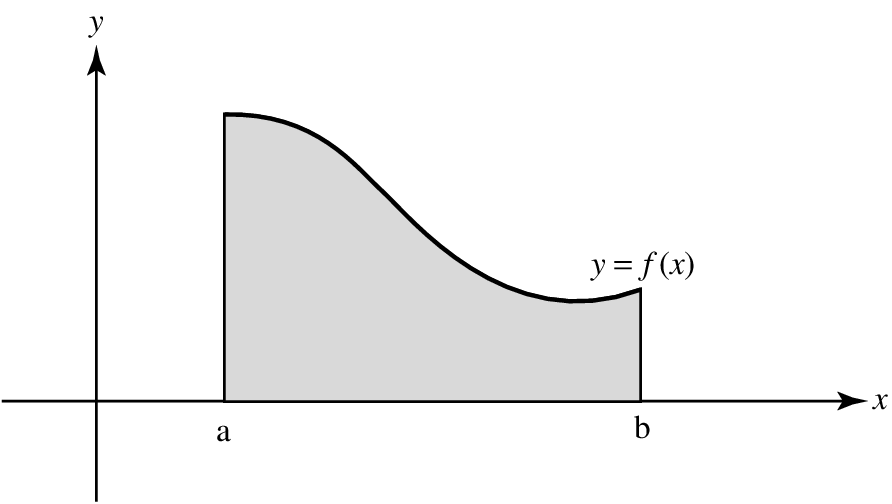
\includegraphics[width=3in,height=1.7in]{png/fig030101.png}
\end{center}
 \vskip6pt
 \refstepcounter{figure}
 \centerline{\bf Figure \thefigure} \label{figure:3.1.1}
 \vskip12pt

For simplicity, suppose that  $f(x)>0$. Then $f(c_j)(x_j-x_{j-1})$ is
the area of a rectangle with base $x_j-x_{j-1}$ and height $f(c_j)$,
 so the Riemann sum
$$
\sum_{j=1}^n f(c_j)(x_j-x_{j-1})
$$
can be interpreted as the sum of the areas of rectangles related to
the curve $y=f(x)$, as shown in Figure~\ref{figure:3.1.2}.

 \vspace*{12pt}
\begin{center}
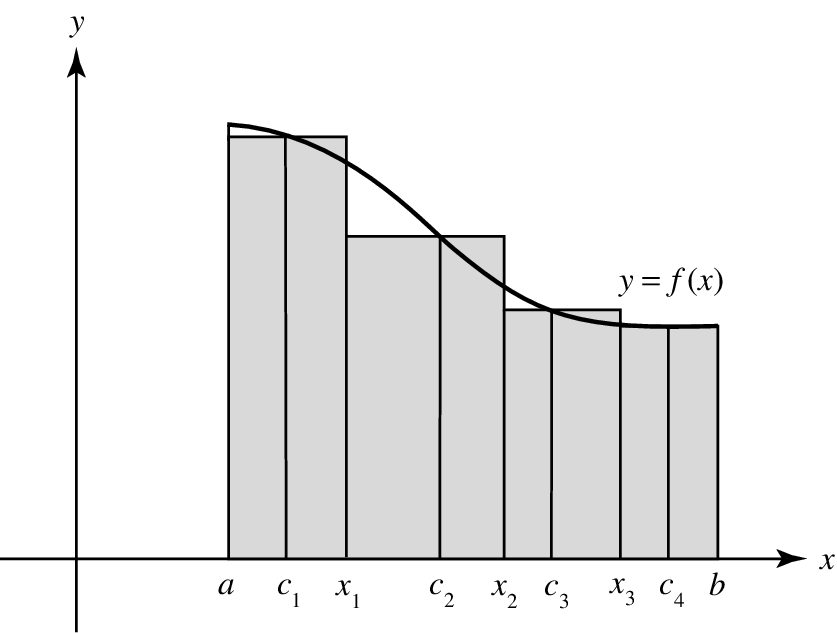
\includegraphics[width=2.85in,height=2.2in]{png/fig030102.png}
\end{center}
 \vskip6pt
 \refstepcounter{figure}
 \centerline{\bf Figure \thefigure} \label{figure:3.1.2}
 \vskip12pt

An apparently
plausible argument, that the Riemann sums approximate the area under
the curve more and more closely as the number of rectangles increases
and the largest of their widths is made smaller, seems to support the
assertion that $\int_a^b f(x)\,dx$ equals the area under the curve.
This argument is useful as a motivation for
Definition~\ref{thmtype:3.1.1}, which without it would seem mysterious.
Nevertheless, the logic is incorrect,
since it is based on the  assumption that the area under the
curve has been previously defined in some other way. Although this is
true for certain curves such as, for example, those consisting of line
segments or circular arcs, it is not true in general. In fact, the
area under a more complicated curve is {\it defined\/} to be equal to
the integral, if the integral exists. That this new definition is
consistent with the old one, where the latter applies, is evidence
that the integral provides a useful generalization of the definition
of area.

\begin{example} \label{example:3.1.3}\rm    Let
$f(x)=x$, $1\le x\le2$
(Figure~\ref{figure:3.1.3}, page \pageref{figure:3.1.3}). The region under
the curve consists of a
square of unit area, surmounted by a triangle of area $1/2$;
thus, the  area of the region is $3/2$. From Example~\ref{example:3.1.2},
$$
\int_1^2 x \,dx=\frac{1}{2}(2^2-1^2)=\frac{3}{2},
$$
 so the integral equals the area under the curve.
\end{example}
\newpage

 \vspace*{12pt}
\begin{center}
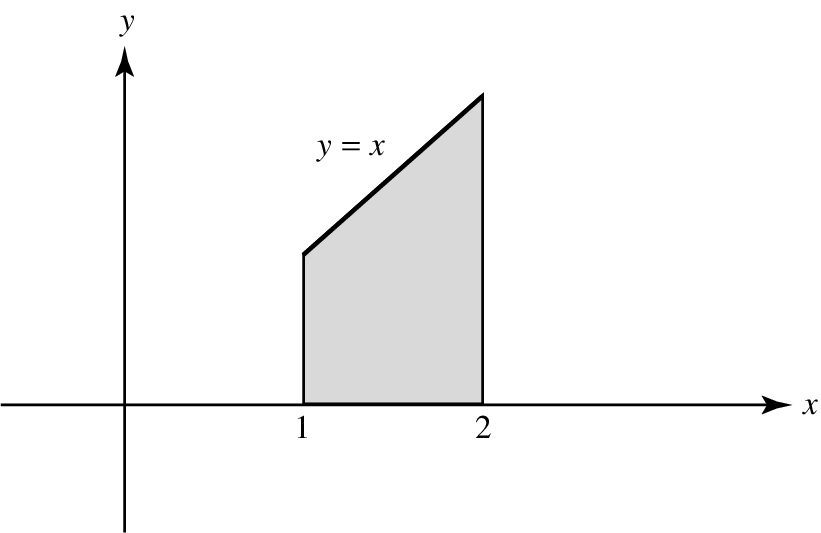
\includegraphics[width=2.8in,height=1.8in]{png/fig030103.png}
\end{center}
 \vskip6pt
 \refstepcounter{figure}
 \centerline{\bf Figure \thefigure} \label{figure:3.1.3}
 \vskip12pt

\begin{center}
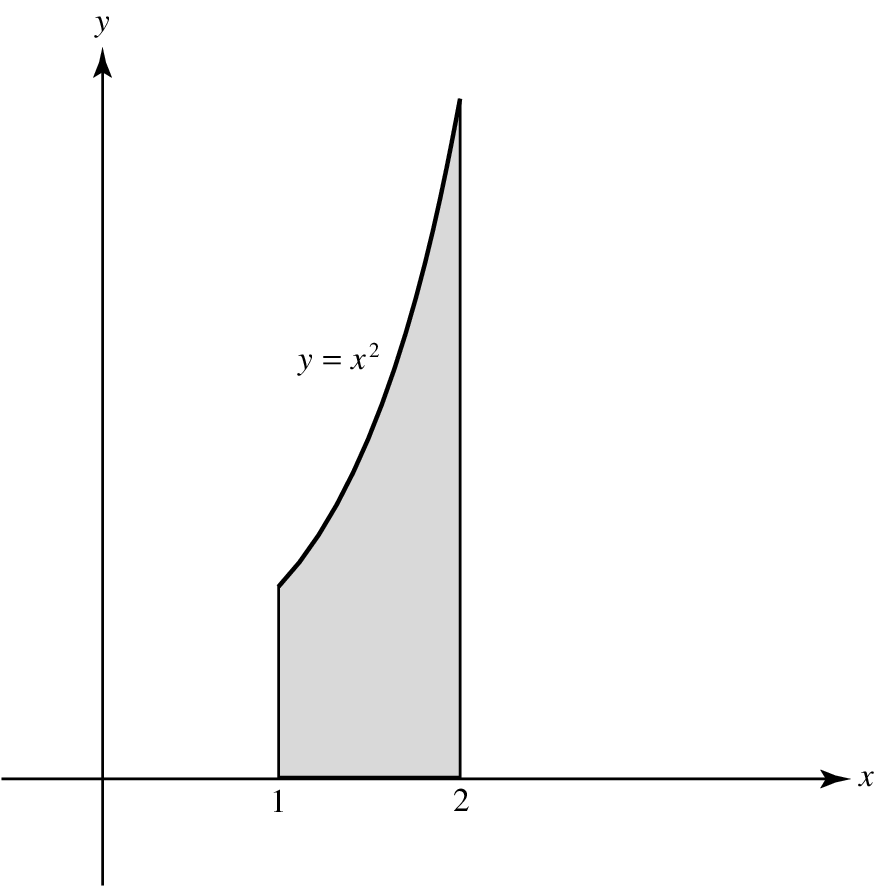
\includegraphics[width=3in,height=3in]{png/fig030104.png}
\end{center}
 \vskip6pt
 \refstepcounter{figure}
 \centerline{\bf Figure \thefigure} \label{figure:3.1.4}
 \vskip12pt

\begin{example} \label{example:3.1.4}\rm   If
$$
f(x)=x^2,\quad 1\le x\le2
$$
(Figure~\ref{figure:3.1.4}), then
$$
\int_1^2 f(x)\,dx=\frac{1}{3}(2^3-1^3)=\frac{7}{3}
$$
(Exercise~\ref{exer:3.1.4}), so we say that the area under the curve
is $7/3$. However, this is the {\it definition\/} of the area
rather than a confirmation of a previously known fact, as in
Example~\ref{example:3.1.3}.
\end{example}

\begin{theorem} \label{thmtype:3.1.2}
If $f$ is unbounded on $[a,b],$ then $f$ is not integrable on
$[a,b].$
\end{theorem}

\proof
 We will show that if $f$ is unbounded on $[a,b]$, $P$ is any
partition of $[a,b]$, and $M>0$, then there are Riemann sums $\sigma$
and $\sigma'$ of $f$ over $P$ such that
\begin{equation} \label{eq:3.1.7}
|\sigma-\sigma'|\ge M.
\end{equation}
We leave it to you (Exercise~\ref{exer:3.1.2}) to complete  the proof by
showing from this that
$f$ cannot satisfy Definition~\ref{thmtype:3.1.1}.

Let
$$
\sigma=\sum_{j=1}^nf(c_j)(x_j-x_{j-1})
$$
be a Riemann sum of $f$ over a partition $P$ of $[a,b]$. There must be
an integer $i$ in $\{1,2, \dots,n\}$ such that
\begin{equation} \label{eq:3.1.8}
|f(c)-f(c_i)|\ge \frac{M }{ x_i-x_{i-1}}
\end{equation}
for some $c$ in $[x_{i-1}x_i]$, because if there were not so,  we
would have
$$
|f(x)-f(c_j)|<\frac{M}{ x_j-x_{j-1}},\quad x_{j-1}\le x\le x_j,\quad
1\le j\le n.
$$
Then
\begin{eqnarray*}
|f(x)|\ar=|f(c_j)+f(x)-f(c_j)|\le|f(c_j)|+|f(x)-f(c_j)|\\
\ar\le |f(c_j)|+\frac{M}{ x_j-x_{j-1}},\quad x_{j-1}\le x\le x_j,\quad
1\le j\le n.
\end{eqnarray*}
which implies that
$$
|f(x)|\le\max_{1\le j\le n}|f(c_j)|+\frac{M}{
x_j-x_{j-1}},
\quad a\le x \le b,
$$
contradicting the assumption that $f$ is unbounded on $[a,b]$.

 Now  suppose that  $c$ satisfies \eqref{eq:3.1.8}, and
consider the Riemann sum
$$
\sigma'=\sum_{j=1}^nf(c'_j)(x_j-x_{j-1})
$$
over the same partition $P$, where
$$
c'_j=\left\{\casespace\begin{array}{ll}
c_j,&j \ne i,\\
c,&j=i.\end{array}\right.
$$

\newpage
\noindent
Since
$$
|\sigma-\sigma'|=|f(c)-f(c_i)|(x_i-x_{i-1}),
$$
\eqref{eq:3.1.8} implies \eqref{eq:3.1.7}.
\bbox

\boxit{Upper and Lower Integrals}
Because of Theorem~\ref{thmtype:3.1.2}, we  consider only bounded
functions throughout the rest of this section.

To prove directly from Definition~\ref{thmtype:3.1.1} that $\int_a^b
f(x)\,dx$ exists, it is necessary to discover its value $L$ in one way
or another and to show that $L$ has the properties required by the
definition. For a specific function it may happen that this can be
done by straightforward calculation, as in Examples~\ref{example:3.1.1}
and \ref{example:3.1.2}. However, this is not so if the objective is to
find general conditions which imply that $\int_a^b f(x)\,dx$ exists.
The following approach avoids the difficulty of having to discover
$L$ in advance, without knowing whether it exists in the first
place, and requires only that we compare two
 numbers that must exist if $f$
is bounded on $[a,b]$. We will see that $\int_a^b f(x)\,dx$ exists
if and only if these two numbers are equal.

\begin{definition} \label{thmtype:3.1.3}
If $f$ is bounded on $[a,b]$ and
$P=\{x_0,x_1, \dots,x_n\}$ is a partition of $[a,b]$, let
\begin{eqnarray*}
M_j\ar=\sup_{x_{j-1}\le x\le x_j}f(x)\\
\arraytext{and}\\
m_j\ar=\inf_{x_{j-1}\le x\le x_j}f(x).
\end{eqnarray*}
The {\it upper sum of $f$ over $P$\/}
 is
$$
S(P)=\sum_{j=1}^n M_j(x_j-x_{j-1}),
$$
and the {\it upper integral of $f$ over\/},
$[a,b]$, denoted by
$$
\overline{\int_a^b} f(x)\,dx,
$$
is  the infimum of all upper sums.  The {\it lower
sum of $f$ over $P$\/}
is
$$
s(P)=\sum_{j=1}^n m_j(x_j-x_{j-1}),
$$
and the {\it lower integral of $f$ over\/}
$[a,b]$, denoted by
$$
\underline{\int_a^b}f(x)\,dx,
$$
is the supremum of all lower sums.
\bbox\end{definition}

\newpage

 If $m\le
f(x)\le M$ for all $x$ in $[a,b]$, then
$$
m(b-a)\le s(P)\le S(P)\le M(b-a)
$$
for every partition $P$; thus, the set of upper sums of $f$ over all
partitions $P$ of $[a,b]$ is bounded, as is the set of lower sums.
Therefore,
Theorems~\ref{thmtype:1.1.3} and \ref{thmtype:1.1.8} imply
that $\overline{\int_a^b}f(x)\,dx$ and
$\underline{\int_a^b}f(x)\,dx$ exist, are unique, and satisfy the
inequalities
$$
m(b-a)\le\overline{\int_a^b} f(x)\,dx\le M(b-a)
$$
and
$$
m(b-a)\le \underline{\int_a^b}f(x)\,dx\le M(b-a).
$$

\begin{theorem}  \label{thmtype:3.1.4}
Let $f$ be bounded on $[a,b]$,  and let $P$
be a partition of $[a,b].$  Then
\begin{alist}
\item % (a)
 The upper sum $S(P)$ of $f$ over $P$ is the supremum
 of the set of all Riemann sums of $f$ over $P.$
\item % (b)
 The lower sum $s(P)$ of $f$ over $P$ is the infimum
 of the set of all Riemann sums of $f$ over $P.$
\end{alist}
\end{theorem}

\proof \part{a} If $P=\{x_0,x_1, \dots,x_n\}$, then
$$
S(P)=\sum_{j=1}^n M_j(x_j-x_{j-1}),
$$
where
$$
M_j=\sup_{x_{j-1}\le x\le x_j}f(x).
$$
An arbitrary Riemann sum of $f$ over $P$ is of the form
$$
\sigma=\sum_{j=1}^n f(c_j)(x_j-x_{j-1}),
$$
where $x_{j-1}\le c_j\le x_j$.
Since $f(c_j)\le M_j$, it follows that $\sigma\le S(P)$.

Now let
$\epsilon>0$ and choose $\overline c_j$ in $[x_{j-1},x_j]$ so that
$$
f(\overline c_j) > M_j -\frac{\epsilon}{ n(x_j-x_{j-1})},\quad 1\le j\le
n.
$$
The Riemann sum produced in this way is
$$
\overline \sigma=\sum_{j=1}^n
f(\overline
c_j)(x_j-x_{j-1})>\sum_{j=1}^n\left[M_j-\frac{\epsilon}{
n(x_j-x_{j-1})})\right](x_j-x_{j-1})=S(P)-\epsilon.
$$
Now  Theorem~\ref{thmtype:1.1.3} implies that
$S(P)$ is the supremum of the set of  Riemann sums of $f$
over $P$.

\part{b} Exercise~\ref{exer:3.1.7}.
\bbox

\newpage

\begin{example} \label{example:3.1.5}\rm    Let
$$
f(x)=\left\{\casespace\begin{array}{ll}
0&\mbox{ if $x$ is irrational}, \\
1&\mbox{ if $x$ is rational},\end{array}\right.
$$
and $P=\{x_0,x_1, \dots,x_n\}$ be a partition of $[a,b]$.  Since every
interval contains both rational and irrational numbers
(Theorems~\ref{thmtype:1.1.6} and  \ref{thmtype:1.1.7}),
$$
m_j=0 \mbox{\quad and \quad} M_j=1,\quad 1\le j\le n.
$$
Hence,
\begin{eqnarray*}
S(P)\ar=\sum_{j=1}^n1\cdot(x_j-x_{j-1})=b-a\\
\arraytext{and}\\
s(P)\ar=\sum_{j=1}^n0\cdot(x_j-x_{j-1})=0.
\end{eqnarray*}
Since all upper sums equal $b-a$ and all lower sums equal $0$,
Definition~\ref{thmtype:3.1.3} implies that
$$
\overline{\int_a^b}f(x)\,dx=b-a \mbox{\quad and \quad}
\underline{\int_a^b}f(x)\,dx=0.
$$
\end{example}

\begin{example} \label{example:3.1.6}\rm  Let $f$ be defined on $[1,2]$ by
$f(x)=0$ if $x$ is irrational and $f(p/q)=1/q$ if $p$ and $q$ are
positive integers with no common factors
(Exercise~\ref{exer:2.2.7}). If $P=\{x_0,x_1, \dots,x_n\}$ is
any partition of $[1,2]$, then $m_j=0$, $1\le j\le n$,
 so
$s(P)=0$; hence,
$$
\underline{\int_1^2} f(x)\,dx=0.
$$
We now show that
\begin{equation} \label{eq:3.1.9}
\overline{\int_1^2}f(x)\,dx=0
\end{equation}
also. Since $S(P)>0$ for every $P$, Definition~\ref{thmtype:3.1.3} implies
that
$$
\overline{\int_1^2}f(x)\,dx\ge0,
$$
 so we need only show that
$$
\overline{\int_1^2}f(x)\,dx\le0,
$$
which will follow if we show that no positive number is less than
every upper sum. To this end, we observe that if $0<\epsilon<2$, then
$f(x) \ge \epsilon/2$ for only finitely many values of $x$ in $[1,2]$.

Let $k$ be the number of such points and let
 $P_0$ be a partition of $[1,2]$ such that
\begin{equation} \label{eq:3.1.10}
\|P_0\|<\frac{\epsilon}{2k}.
\end{equation}

\newpage
\noindent
Consider the upper sum
$$
S(P_0)=\sum_{j=1}^nM_j(x_j-x_{j-1}).
$$
There are at most $k$ values of $j$ in this sum for which $M_j\ge
\epsilon/2$, and $M_j\le1$ even for these. The contribution of these
terms to the sum is less than $k(\epsilon/2k)=\epsilon/2$, because of
\eqref{eq:3.1.10}. Since $M_j<\epsilon/2$ for all other values of $j$,
the sum of the other terms is  less than
$$
\frac{\epsilon}{2}\sum_{j=1}^n(x_j-x_{j-1})=\frac{\epsilon}{
2}(x_n-x_0)=\frac{\epsilon}{2}(2-1)=\frac{\epsilon}{2}.
$$
Therefore, $S(P_0)<\epsilon$ and, since $\epsilon$ can be chosen as small
as we wish, no positive number is less than all upper sums.  This proves
\eqref{eq:3.1.9}.
\bbox\end{example}

The motivation for Definition~\ref{thmtype:3.1.3} can be seen by again
considering the idea of area under a curve. Figure~\ref{figure:3.1.5}
shows the graph of a positive function $y=f(x)$, $a\le x\le b$, with
$[a,b]$ partitioned into four subintervals.

 \vspace*{12pt}
\begin{center}
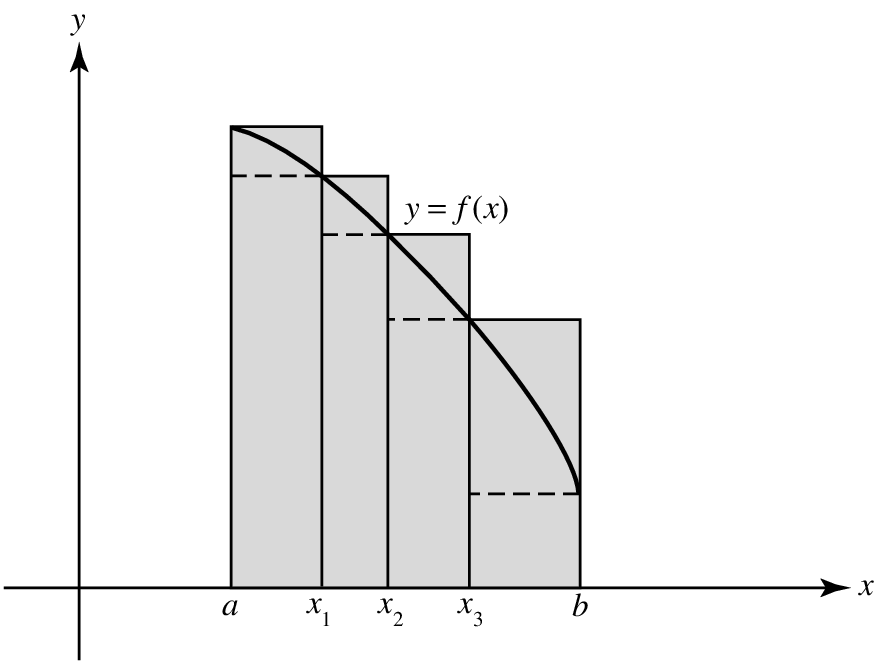
\includegraphics[width=3in,height=2.3in]{png/fig030105.png}
\end{center}
 \vskip6pt
 \refstepcounter{figure}
 \centerline{\bf Figure \thefigure} \label{figure:3.1.5}
 \vskip12pt

\noindent
The upper and lower sums
of $f$ over this partition can be interpreted as the sums of the areas
of the rectangles surmounted by the solid and dashed lines,
respectively. This indicates that a sensible definition of area $A$
under the curve must admit the inequalities
$$
s(P)\le A\le S(P)
$$
for every partition $P$ of $[a,b]$. Thus, $A$ must be an upper bound
for all lower sums and a lower bound for all upper sums of $f$ over
partitions of $[a,b]$. If
\begin{equation} \label{eq:3.1.11}
\overline{\int_a^b}f(x)\,dx=\underline{\int_a^b}f(x)\,dx,
\end{equation}
\newpage

\noindent
there is only one number, the common value of the upper and lower
integrals, with this property, and we define $A$ to be that number;
if \eqref{eq:3.1.11} does not hold, then $A$ is not defined. We will see
below that this definition of area is consistent with the definition
stated earlier in terms of Riemann sums.

\begin{example} \label{example:3.1.7}\rm  Returning to
Example~\ref{example:3.1.3}, consider the function
$$
f(x)=x,\quad 1\le x\le2.
$$
If $P=\{x_0,x_1, \dots,x_n\}$ is a partition of $[1,2]$, then, since
$f$ is increasing,
$$
M_j=f(x_j)=x_j \mbox{\quad and \quad} m_j=f(x_{j-1})=x_{j-1}.
$$
Hence,
\begin{eqnarray}
S(P)\ar=\sum_{j=1}^nx_j(x_j-x_{j-1})\label{eq:3.1.12}\\
\arraytext{and}\nonumber\\
s(P)\ar=\sum_{j=1}^nx_{j-1}(x_j-x_{j-1})\label{eq:3.1.13}.
\end{eqnarray}
By writing
$$
x_j=\frac{x_j+x_{j-1}}{2}+\frac{x_j-x_{j-1}}{2},
$$
we see from \eqref{eq:3.1.12} that
\begin{equation} \label{eq:3.1.14}
\begin{array}{rcl}
S(P)\ar=\dst{\frac{1}{2} \sum_{j=1}^n(x^2_j-x^2_{j-1})+\frac{1}{
2}\sum_{j=1}^n(x_j-x_{j-1})^2} \\
\ar=\dst{\frac{1}{2}(2^2-1^2)+\frac{1}{2}\sum_{j=1}^n(x_j-x_{j-1})^2}.
\end{array}
\end{equation}
Since
$$
0<\sum_{j=1}^n(x_j-x_{j-1})^2\le
\|P\|\sum_{j=1}^n(x_j-x_{j-1})=\|P\|(2-1),
$$
\eqref{eq:3.1.14} implies that
$$
\frac{3}{2}<S(P)\le \frac{3}{2}+\frac{\|P\|}{2}.
$$
Since $\|P\|$ can be made as small as we please,
Definition~\ref{thmtype:3.1.3} implies that
$$
\overline{\int_a^b} f(x)\,dx=\frac{3}{2}.
$$
A similar argument starting from \eqref{eq:3.1.13} shows that
$$
\frac{3}{2}-\frac{\|P\|}{2}\le s(P)<\frac{3}{2},
$$
\newpage
\noindent
so
$$
\underline{\int_a^b}f(x)\,dx=\frac{3}{2}.
$$
Since the upper and lower integrals both equal $3/2$, the area
under the curve is $3/2$ according to our new definition. This
is consistent with the result in Example~\ref{example:3.1.3}.
\end{example}

\boxit{The Riemann--Stieltjes Integral}
The {\it Riemann--Stieltjes integral\/}
 is an important
generalization of
the Riemann integral. We define it here, but confine our study of it
to the exercises in this and other sections of this chapter.

\begin{definition} \label{thmtype:3.1.5}
Let $f$ and $g$ be defined on $[a,b]$. We say that $f$ is
{\it Riemann}--\href{http://www-history.mcs.st-and.ac.uk/Mathematicians/Stieltjes.html}
{\it Stieltjes}
{\it integrable with respect to $g$ on\/}
$[a,b]$
if there
is a number $L$ with the following property: For every $\epsilon>0$,
there is a $\delta>0$ such that
\begin{equation} \label{eq:3.1.15}
\left|\sum_{j=1}^n f(c_j)\left[g(x_j)-g(x_{j-1})\right]-L \right|<
\epsilon,
\end{equation}
provided only that $P=\{x_0,x_1, \dots,x_n\}$ is a partition of $[a,b]$
such that $\|P\|<\delta$ and
$$
x_{j-1}\le c_j\le x_j,\quad j=1,2, \dots,n.
$$
In this case, we say that $L$ is {\it the Riemann--Stieltjes integral
of
$f$ with respect to $g$ over\/}
$[a,b]$, and write
$$
\int_a^b f(x)\,dg (x)=L.
$$

The sum
$$
\sum_{j=1}^n f(c_j)\left[g(x_j)-g(x_{j-1})\right]
$$
in \eqref{eq:3.1.15} is  {\it a Riemann--Stieltjes sum of $f$
with respect to $g$ over the partition~$P$\/}.
\end{definition}

\exercises
\begin{exerciselist}

\item\label{exer:3.1.1} Show that there cannot be more than one number $L$
that satisfies Definition~\ref{thmtype:3.1.1}.

\item\label{exer:3.1.2}
\begin{alist}
\item % (a)
 Prove:  If $\int_a^bf(x)\,dx$ exists, then for every
$\epsilon>0$, there is a $\delta>0$ such that $|\sigma_1-\sigma_2|<
\epsilon$ if $\sigma_1$ and $\sigma_2$ are Riemann sums of $f$ over
partitions $P_1$ and $P_2$ of $[a,b]$ with norms less than $\delta$.

\newpage
\item % (b)
Suppose that  there is an $M>0$ such that, for every $\delta>0$, there are
Riemann sums $\sigma_1$ and $\sigma_2$ over a partition $P$ of $[a,b]$
with $\|P\|<\delta$ such that $|\sigma_1-\sigma_2|\ge M$. Use \part{a}
to prove that $f$ is not integrable over $[a,b]$.
\end{alist}

\vskip2pt
\item\label{exer:3.1.3}
Suppose that  $\int_a^bf(x)\,dx$ exists and
there is a number $A$ such that, for every $\epsilon>0$ and
$\delta>0$,
there is a partition $P$ of $[a,b]$ with $\|P\|<\delta$ and a Riemann
sum $\sigma$ of $f$ over $P$ that satisfies the inequality
$|\sigma-A|<\epsilon$. Show that $\int_a^b f(x)\,dx=A$.

\vskip2pt
\item\label{exer:3.1.4}
Prove directly from Definition~\ref{thmtype:3.1.1}
that
$$
\int_a^b x^2\,dx=\frac{b^3-a^3}{3}.
$$
Do not assume in advance that the integral exists. The proof of this
is part of the problem. \hint{Let $P=\{x_0,x_2, \dots,x_n\}$ be
an arbitrary partition of $[a,b].$
Use the mean value theorem to show that
$$
\frac{b^3-a^3}{3}=\sum_{j=1}^nd^2_j(x_j-x_{j-1})
$$
for some points $d_1,$ \dots, $d_n,$ where $x_{j-1}<d_j<x_j$.
Then relate this sum to arbitrary Riemann sums for $f(x)=x^2$ over
 $P.$}

\vskip2pt
\item\label{exer:3.1.5} Generalize the proof of Exercise~\ref{exer:3.1.4} to
show directly from Definition~\ref{thmtype:3.1.1} that
$$
\int_a^b x^m\,dx=\frac{b^{m+1}-a^{m+1}}{ m+1}
$$
if $m$ is an integer $\ge0$.

\vskip2pt
\item\label{exer:3.1.6}
Prove directly from Definition~\ref{thmtype:3.1.1} that $f(x)$ is
integrable on $[a,b]$ if and only if $f(-x)$ is integrable on
$[-b,-a]$, and,  in this case,
$$
\int_a^b f(x)\,dx=\int_{-b}^{-a}f(-x)\,dx.
$$

\vskip2pt
\item\label{exer:3.1.7}
Let $f$ be bounded on $[a,b]$  and let $P$
be a partition of $[a,b]$.  Prove:
 The lower sum $s(P)$ of $f$ over $P$ is the infimum
 of the set of all Riemann sums of $f$ over $P$.

\vskip2pt
\item\label{exer:3.1.8}
Let $f$ be defined on $[a,b]$  and let $P=\{x_0,x_1, \dots,x_n\}$
be a partition of $[a,b]$.
\begin{alist}
\item % (a)
 Prove:  If $f$ is continuous on $[a,b]$, then $s(P)$ and
$S(P)$ are Riemann sums of $f$ over~$P$.
\item % (b)
 Name another class of functions for which the conclusion of
\part{a} is valid.
\item % (c)
 Give an example where $s(P)$ and $S(P)$ are not Riemann
sums of $f$ over~$P$.
\end{alist}

\newpage
\item\label{exer:3.1.9}
 Find $\underline{\int_0^1}f(x)\,dx$ and
$\overline{\int_0^1}f(x)\,dx$ if

\hskip-.5em
\begin{tabular}{cc}
\part{a} $f(x)=\dst\left\{\casespace\begin{array}{rl}
 x&\mbox{ if $x$ is rational},\\
-x&\mbox{ if $x$ is irrational}.\end{array}\right.$&
\part{b} $f(x)=\dst\left\{\casespace\begin{array}{rl}
 1&\mbox{ if $x$ is rational},\\
x&\mbox{ if $x$ is irrational}.\end{array}\right.$
\end{tabular}

\item\label{exer:3.1.10} Given that $\int_a^be^x\,dx$ exists, evaluate it
by using the formula
$$
1+r+r^2+\cdots+r^n=\frac{1-r^{n+1}}{1-r} \quad (r \ne1)
$$
to calculate certain Riemann sums.  \hint{See
Exercise~$\ref{exer:3.1.3}.$}

\item\label{exer:3.1.11} Given that $\int_0^b\sin x \,dx$ exists, evaluate
it by using the identity
$$
\cos(j-1)\theta-\cos(j+1)\theta=2\sin\theta\sin j\theta
$$
to calculate certain Riemann sums.  \hint{See
Exercise~$\ref{exer:3.1.3}.$}

\item\label{exer:3.1.12} Given that $\int_0^b\cos x\,dx$ exists, evaluate
it by using the identity
$$
\sin(j+1)\theta-\sin(j-1)\theta=2\sin\theta\cos j \theta
$$
to calculate certain Riemann sums.  \hint{See
Exercise~$\ref{exer:3.1.3}.$}

\item\label{exer:3.1.13}
Show that if $g(x)=x+c$ ($c$=constant), then  $\int_a^b f(x)\,dg(x)$
exists if and only if $\int_a^bf(x)\,dx$ exists, in which case
$$
\int_a^b f(x)\,dg(x)=\int_a^bf(x)\,dx.
$$

\item\label{exer:3.1.14}
Suppose  that $-\infty<a<d<c<\infty$  and
$$
g(x)=\left\{\casespace\begin{array}{ll} g_1,&a<x<d,\\
g_2,&d<x<b,\end{array}\right. \mbox{($g_1,g_2=$ constants),
\quad}
$$
and let $g(a)$, $g(b)$, and $g(d)$ be arbitrary. Suppose that  $f$ is
defined on $[a,b]$, continuous from the right at $a$ and from the left
at $b$, and continuous at $d$. Show that $\int_a^b f(x)\,dg(x)$
exists, and find its value.

\item\label{exer:3.1.15}
 Suppose that  $-\infty<a=a_0<a_1<\cdots<a_p=b<\infty$, let $g(x)=g_m$
(constant) on $(a_{m-1},a_m)$, $1\le m\le p$, and
let
$g(a_0)$,
$g(a_1)$, \dots, $g(a_p)$ be arbitrary. Suppose that  $f$ is defined on
$[a,b]$, continuous from the right at $a$ and from the left at $b$,
and continuous at $a_1$, $a_2$, \dots, $a_{p-1}$. Evaluate
$\int_a^bf(x)\,dg(x)$. \hint{See Exercise~$\ref{exer:3.1.14}.$}

\item\label{exer:3.1.16}
\begin{alist}
\item % (a)
Give an example where $\int_a^bf(x)\,dg(x)$ exists even though $f$ is
unbounded on $[a,b]$. (Thus, the analog of Theorem~\ref{thmtype:3.1.2}
does not hold for the Riemann--Stieltjes integral.)
\item % (b)
 State and prove an analog of Theorem~\ref{thmtype:3.1.2} for the case
where
$g$ is increasing.
\end{alist}

\newpage
\item\label{exer:3.1.17} For the case where $g$ is nondecreasing and $f$
is bounded on $[a,b]$, define upper and lower Riemann--Stieltjes
integrals in a way analogous to Definition~\ref{thmtype:3.1.3}.

\label{sectionend:\thesection}
\end{exerciselist}

\currentpdfbookmark{Section 3.2 Existence of the Integral}{section:3.2}
\newsection{2}
{Integral Calculus of Functions of One Variable}
{Existence of the Integral}

\renewcommand{\thissection}{\sectiontitle{EXISTENCE OF THE INTEGRAL}}
\thissection

\noindent
The following lemma is the starting point for our study of the
integrability of a bounded function $f$ on a closed interval $[a,b]$.

\begin{lemma} \label{thmtype:3.2.1}
Suppose that
\begin{equation} \label{eq:3.2.1}
|f(x)|\le M,\quad a\le x\le b,
\end{equation}
and let $P'$ be a partition of $[a,b]$ obtained by adding $r$ points to a
partition $P=\{x_0,x_1, \dots,x_n\}$ of $[a,b].$  Then
\begin{eqnarray}
S(P)\ge S(P')\ar\ge S(P)-2Mr\|P\|\label{eq:3.2.2}\\
\arraytext{and}\nonumber\\
s(P)\le s(P')\ar\le s(P)+2Mr\|P\|\label{eq:3.2.3}.
\end{eqnarray}
\end{lemma}

\proof
 We will prove \eqref{eq:3.2.2} and leave the proof of \eqref{eq:3.2.3}
to you (Exercise~\ref{exer:3.2.1}).
First suppose that $r=1$, so
 $P'$ is obtained by  adding one point $c$ to the
partition
$P=\{x_0,x_1, \dots,x_n\}$; then
$x_{i-1}<c<x_i$ for some $i$ in $\{1,2, \dots,n\}$.
 If $j \ne i$,  the product
$M_j(x_j-x_{j-1})$ appears in both $S(P)$ and $S(P')$ and cancels out
of the difference $S(P)-S(P')$. Therefore, if
$$
M_{i1}=\sup_{x_{i-1}\le x\le c}f(x)  \mbox{\quad and \quad}
M_{i2}= \sup_{c\le x\le x_i}f(x),
$$
then
\begin{equation} \label{eq:3.2.4}
\begin{array}{rcl}
S(P)-S(P')\ar=M_i(x_i-x_{i-1})-M_{i1}(c-x_{i-1})-M_{i2}(x_i-c)
\\[2\jot]
\ar=(M_i-M_{i1})(c-x_{i-1})+(M_i-M_{i2})(x_i-c).
\end{array}
\end{equation}
Since \eqref{eq:3.2.1} implies that
$$
0\le M_i-M_{ir}\le2M,\quad r=1,2,
$$
 \eqref{eq:3.2.4} implies that
$$
0\le S(P)-S(P')\le2M(x_i-x_{i-1})\le2M\|P\|.
$$
This proves \eqref{eq:3.2.2} for $r=1$.

Now suppose that $r>1$ and $P'$  is obtained by adding points $c_1$,
$c_2$, \dots, $c_r$ to $P$. Let $P^{(0)}=P$ and, for $j\ge1$, let
$P^{(j)}$ be the partition of $[a,b]$ obtained by adding $c_j$
to $P^{(j-1)}$. Then the result just proved implies that
$$
0\le S(P^{(j-1)})-S(P^{(j)})\le2M\|P^{(j-1)}\|,\quad 1\le j\le r.
$$
\newpage
\noindent
Adding these inequalities and taking account of cancellations
 yields
\begin{equation} \label{eq:3.2.5}
0\le
S(P^{(0)})-S(P^{(r)})\le2M(\|P^{(0)}\|+\|P^{(1)}\|+\cdots+\|P^{(r-1)}\|).
\end{equation}
Since $P^{(0)}=P$, $P^{(r)}=P'$, and $\|P^{(k)}\|\le\|P^{(k-1)}\|$
for $1\le k\le r-1$, \eqref{eq:3.2.5} implies that
$$
0\le S(P)-S(P')\le 2Mr\|P\|,
$$
which is equivalent to \eqref{eq:3.2.2}.
\bbox

\begin{theorem} \label{thmtype:3.2.2}
If $f$ is bounded on $[a,b],$ then
\begin{equation} \label{eq:3.2.6}
\underline{\int_a^b}f(x)\,dx\le\overline{\int_a^b}f(x)\,dx.
\end{equation}
\end{theorem}

\proof
Suppose that $P_1$ and $P_2$ are partitions of $[a,b]$ and $P'$ is a
refinement of both. Letting $P=P_1$ in \eqref{eq:3.2.3} and $P=P_2$ in
\eqref{eq:3.2.2} shows that
$$
s(P_1)\le s(P') \mbox{\quad and \quad} S(P')\le S(P_2).
$$
Since $s(P')\le S(P')$, this implies that
$s(P_1)\le S(P_2)$.
Thus, every lower sum is a lower bound for the set of all upper sums.
Since $\overline{\int_a^b}f(x)\,dx$ is the infimum of
this set, it follows that
$$
s(P_1)\le\overline{\int_a^b}f(x)\,dx
$$
for every partition $P_1$ of $[a,b]$. This means that
$\overline{\int_a^b}
f(x)\,dx$ is an upper bound for the set of all lower sums. Since
$\underline{\int_a^b} f(x)\,dx$ is the supremum of this set,
this implies \eqref{eq:3.2.6}.
\bbox

\begin{theorem} \label{thmtype:3.2.3}
If $f$ is integrable on $[a,b],$ then
$$
\underline{\int_a^b}f(x)\,dx=\overline{\int_a^b}f(x)\,dx=\int_a^b
f(x)\,dx.
$$
\end{theorem}

\proof
We prove that
$\overline{\int_a^b}f(x)\,dx=\int_a^bf(x)\,dx$ and leave it to you to
show that
$\underline{\int_a^b}f(x)\,dx=\int_a^bf(x)\,dx$
(Exercise~\ref{exer:3.2.2}).

 Suppose that $P$ is a partition of $[a,b]$
and $\sigma$ is a Riemann sum of $f$ over $P$.
Since
\begin{eqnarray*}
\overline{\int_a^b}f(x)\,dx-\int_a^b f(x)\,dx\ar=
\left(\overline{\int_a^b}f(x)\,dx-S(P)\right)+(S(P)-\sigma)
\\[2\jot]
&&+\left(\sigma-\int_a^b f(x)\ dx\right),
\end{eqnarray*}
\newpage
\noindent
the triangle inequality implies that
\begin{equation} \label{eq:3.2.7}
\begin{array}{rcl}
\dst{\left|\overline{\int_a^b}f(x)\,dx-\int_a^b f(x)\,dx \right|}\ar\le
\dst{\left|\overline{\int_a^b}f(x)\,dx-S(P)\right|+|S(P)-\sigma|}
\\[2\jot]
&&+\dst{\left|\sigma-\int_a^b f(x)\ dx\right|}.
\end{array}
\end{equation}
Now suppose that $\epsilon>0$.
 From Definition~\ref{thmtype:3.1.3}, there is
a partition $P_0$ of $[a,b]$ such that
\begin{equation} \label{eq:3.2.8}
\overline{\int_a^b} f(x)\,dx\le S(P_0)<
\overline{\int_a^b}f(x)\,dx+\frac{\epsilon}{3}.
\end{equation}
From Definition~\ref{thmtype:3.1.1}, there is a $\delta>0$ such that
\begin{equation} \label{eq:3.2.9}
\left|\sigma-\int_a^bf(x)\,dx\right|<\frac{\epsilon}{3}
\end{equation}
if $\|P\|<\delta$. Now suppose that $\|P\|<\delta$ and $P$ is a
refinement of $P_0$. Since $S(P)\le S(P_0)$ by Lemma~\ref{thmtype:3.2.1},
\eqref{eq:3.2.8}  implies that
$$
\overline{\int_a^b} f(x)\,dx\le S(P)<
\overline{\int_a^b}f(x)\,dx+\frac{\epsilon}{3},
$$
so
\begin{equation} \label{eq:3.2.10}
\left|S(P)-\overline{\int_a^b}f(x)\,dx\right|<\frac{\epsilon}{3}
\end{equation}
in addition to \eqref{eq:3.2.9}. Now \eqref{eq:3.2.7}, \eqref{eq:3.2.9}, and
\eqref{eq:3.2.10} imply that
\begin{equation} \label{eq:3.2.11}
\left|\overline{\int_a^b} f(x)\,dx-\int_a^b f(x)\,dx\right|<
\frac{2\epsilon}{3}+|S(P)-\sigma|
\end{equation}
for every Riemann sum $\sigma$ of $f$ over $P$.  Since $S(P)$ is the
supremum of these Riemann sums
(Theorem~\ref{thmtype:3.1.4}), we may choose
$\sigma$ so that
$$
|S(P)-\sigma|<\frac{\epsilon}{3}.
$$
Now \eqref{eq:3.2.11} implies that
$$
\left|\overline{\int_a^b} f(x)\,dx-\int_a^b f(x)\,dx \right|<
\epsilon.
$$
Since $\epsilon$ is an arbitrary positive number, it follows that
$$
\overline{\int_a^b}f(x)\,dx=\int_a^b f(x)\,dx.
$$
\vskip-6.5ex\bbox\vskip6.5ex

\begin{lemma} \label{thmtype:3.2.4}
If $f$ is bounded on $[a,b]$ and
 $\epsilon>0,$   there is a $\delta>0$ such that
\begin{equation} \label{eq:3.2.12}
\overline{\int_a^b}f(x)\,dx\le
S(P)<\overline{\int_a^b}f(x)\,dx+\epsilon
\end{equation}
and
$$
\underline{\int_a^b} f(x)\,dx\ge s(P)>\underline{\int_a^b}
f(x)\,dx-\epsilon
$$
if $\|P\|<\delta$.
\end{lemma}

\proof
 We show that \eqref{eq:3.2.12} holds if $\|P\|$ is sufficiently
small, and leave the rest of the proof to you (Exercise~\ref{exer:3.2.3}).

The first inequality in \eqref{eq:3.2.12} follows immediately from
Definition~\ref{thmtype:3.1.3}.
 To establish the second inequality,
suppose that $|f(x)|\le K$ if $a\le x\le b$. From
Definition~\ref{thmtype:3.1.3}, there is a partition $P_0=
\{x_0,x_1, \dots,x_{r+1}\}$ of $[a,b]$ such that
\begin{equation} \label{eq:3.2.13}
S(P_0)<\overline{\int_a^b}f(x)\,dx+\frac{\epsilon}{2}.
\end{equation}
If $P$ is any partition of $[a,b]$, let $P'$ be constructed from the
partition points of $P_0$ and $P$. Then
\begin{equation} \label{eq:3.2.14}
S(P')\le S(P_0),
\end{equation}
by Lemma~\ref{thmtype:3.2.1}. Since $P'$ is obtained by adding at most
$r$ points to $P$, Lemma~\ref{thmtype:3.2.1} implies that
\begin{equation} \label{eq:3.2.15}
S(P')\ge S(P)-2Kr\|P\|.
\end{equation}
 Now \eqref{eq:3.2.13}, \eqref{eq:3.2.14}, and \eqref{eq:3.2.15}
imply that
\begin{eqnarray*}
S(P)\ar\le  S(P')+2Kr\|P\|\\
\ar\le  S(P_0)+2Kr\|P\|\\
&<&\overline{\int_a^b} f(x)\,dx+\frac{\epsilon}{2}+2Kr\|P\|.
\end{eqnarray*}
 Therefore, \eqref{eq:3.2.12} holds if
$$
\|P\|<\delta=\frac{\epsilon}{4Kr}.
$$
\vskip-4.5ex\bbox\vskip4.5ex

\begin{theorem} \label{thmtype:3.2.5}
If $f$ is bounded on $[a,b]$ and
\begin{equation} \label{eq:3.2.16}
\underline{\int_a^b} f(x)\,dx=\overline{\int_a^b}f(x)\,dx=L,
\end{equation}
then $f$ is integrable on $[a,b]$ and
\begin{equation} \label{eq:3.2.17}
\int_a^b f(x)\,dx=L.
\end{equation}
\end{theorem}

\newpage

\proof
 If $\epsilon>0$, there is a $\delta>0$ such that
\begin{equation} \label{eq:3.2.18}
\underline{\int_a^b}f(x)\,dx-\epsilon<s(P)\le S(P)<
\overline{\int_a^b}f(x)\,dx+\epsilon
\end{equation}
if $\|P\|<\delta$ (Lemma~\ref{thmtype:3.2.4}). If
$\sigma$ is a Riemann sum of  $f$ over $P$, then
$$
s(P)\le \sigma\le S(P),
$$
so \eqref{eq:3.2.16} and \eqref{eq:3.2.18} imply that
$$
L-\epsilon<\sigma<L+\epsilon
$$
if $\|P\|<\delta$. Now
Definition~\ref{thmtype:3.1.1} implies \eqref{eq:3.2.17}.
\bbox

Theorems~\ref{thmtype:3.2.3} and \ref{thmtype:3.2.5}
imply the following theorem.

\begin{theorem} \label{thmtype:3.2.6}
A bounded function
$f$ is integrable on $[a,b]$ if and only if
$$
\underline{\int_a^b}f(x)\,dx=\overline{\int_a^b}f(x)\,dx.
$$
\end{theorem}

The next theorem translates this into a test that can be
conveniently applied.

\begin{theorem} \label{thmtype:3.2.7}
If $f$ is bounded on $[a,b],$ then $f$ is integrable on $[a,b]$
 if and only if for each $\epsilon>0$ there is
a partition $P$ of $[a,b]$ for which
\begin{equation} \label{eq:3.2.19}
S(P)-s(P)<\epsilon.
\end{equation}
\end{theorem}

\proof
We leave it to you (Exercise~\ref{exer:3.2.4}) to show that if $\int_a^b
f(x)\,dx$ exists, then \eqref{eq:3.2.19} holds for $\|P\|$ sufficiently
small. This implies that the stated condition is necessary for
integrability. To show that it is sufficient, we observe that since
$$
s(P)\le \underline{\int_a^b}f(x)\,dx\le\overline{\int_a^b}f(x)\,dx\le
S(P)
$$
for all $P$, \eqref{eq:3.2.19} implies that
$$
0\le\overline{\int_a^b} f(x)\,dx-\underline{\int_a^b}f(x)\,dx<
\epsilon.
$$
Since $\epsilon$ can be any positive number, this implies that
$$
\overline{\int_a^b} f(x)\,dx=\underline{\int_a^b} f(x)\,dx.
$$
Therefore, $\int_a^b f(x)\,dx$ exists, by Theorem~\ref{thmtype:3.2.5}.
\bbox

The next two theorems are important applications of
Theorem~\ref{thmtype:3.2.7}.

\newpage


\begin{theorem} \label{thmtype:3.2.8}
If $f$ is continuous on $[a,b],$
then $f$ is integrable on $[a,b]$.
\end{theorem}

\proof Let $P=\{x_0,x_1, \dots,x_n\}$ be a partition of $[a,b]$. Since
$f$ is continuous on $[a,b]$, there are points $c_j$ and $c'_j$ in
$[x_{j-1},x_j]$ such that
$$ f(c_j)=M_j=\sup_{x_{j-1}\le x\le x_j}f(x)
$$
and
$$
f(c'_j)=m_j=\inf_{x_{j-1}\le x\le x_j}f(x)
$$
(Theorem~\ref{thmtype:2.2.9}).
Therefore,
\begin{equation} \label{eq:3.2.20}
S(P)-s(P)=\sum_{j=1}^n\left[f(c_j)-f(c'_j)\right](x_j-x_{j-1}).
\end{equation}
Since $f$ is uniformly continuous on $[a,b]$
(Theorem~\ref{thmtype:2.2.12}), there is for each $\epsilon>0$
a
$\delta>0$ such that
 $$
|f(x')-f(x)|<\frac{\epsilon}{ b-a}
 $$
 if $x$ and $x'$ are
in $[a,b]$ and $|x-x'|<\delta$. If $\|P\|<\delta$, then
$|c_j-c'_j|<\delta$ and, from \eqref{eq:3.2.20},
$$
 S(P)-s(P)<\frac{\epsilon}{ b-a}
\sum_{j=1}^n(x_j-x_{j-1})=\epsilon.
$$
Hence, $f$ is integrable
on $[a,b]$, by Theorem~\ref{thmtype:3.2.7}.
\bbox

\begin{theorem} \label{thmtype:3.2.9}
If $f$ is monotonic on $[a,b],$ then $f$ is integrable on $[a,b]$.
\end{theorem}

\proof
Let $P=\{x_0,x_1, \dots,x_n\}$ be a partition of $[a,b]$. Since
 $f$ is nondecreasing,
\begin{eqnarray*}
f(x_j)\ar=M_j=\sup_{x_{j-1}\le x\le x_j}f(x)\\
\arraytext{and}\\
f(x_{j-1})\ar=m_j=\inf_{x_{j-1}\le x\le x_j}f(x).
\end{eqnarray*}
Hence,
$$
S(P)-s(P)=\sum_{j=1}^n(f(x_j)-f(x_{j-1})) (x_j-x_{j-1}).
$$
Since $0<x_j-x_{j-1}\le \|P\|$ and $f(x_j)-f(x_{j-1})\ge0$,
\begin{eqnarray*}
S(P)-s(P)\ar\le  \|P\| \sum_{j=1}^n(f(x_j)-f(x_{j-1})) \\
\ar=\|P\|(f(b)-f(a)).
\end{eqnarray*}
\newpage
\noindent
Therefore,
$$
S(P)-s(P)<\epsilon\mbox{\quad if \quad}
\|P\|(f(b)-f(a))<\epsilon,
$$
 so $f$ is integrable on $[a,b]$, by Theorem~\ref{thmtype:3.2.7}.

The proof for nonincreasing $f$ is similar.
\bbox

We will also use Theorem~\ref{thmtype:3.2.7} in the next section to
establish properties of the integral. In Section~3.5 we
will study more general conditions for integrability.

\exercises
\begin{exerciselist}

\item\label{exer:3.2.1} Complete the proof of Lemma~\ref{thmtype:3.2.1} by
verifying Eqn.~\eqref{eq:3.2.3}.

\item\label{exer:3.2.2}  Show that if $f$ is integrable on $[a,b]$, then
$$
\underline{\int_a^b}f(x)\,dx=\int_a^b f(x)\,dx.
$$

\item\label{exer:3.2.3}
Prove: If $f$ is bounded on $[a,b]$, there
is for each $\epsilon>0$ a $\delta>0$ such that
$$
\underline{\int_a^b} f(x)\,dx\ge \underline{\int_a^b}
f(x)\,dx-\epsilon<s(P)
$$
if $\|P\|<\delta$.

\item\label{exer:3.2.4}
Prove: If $f$ is integrable on $[a,b]$ and
$\epsilon>0$, then $S(P)-s(P)<\epsilon$ if $\|P\|$ is sufficiently
small. \hint{Use Theorem~$\ref{thmtype:3.1.4}.$}

\item\label{exer:3.2.5} Suppose that $f$ is integrable and $g$ is bounded
on
$[a,b]$, and $g$ differs from $f$ only at points in a set $H$ with the
following property: For each $\epsilon>0$, $H$ can be covered by a
finite number of closed subintervals of $[a,b]$, the sum of whose
lengths is less than $\epsilon$. Show that $g$ is integrable on
$[a,b]$ and that
$$
\int_a^b g(x)\,dx=\int_a^b f(x)\,dx.
$$
\hint{Use Exercise~$\ref{exer:3.1.3}.$}

\item\label{exer:3.2.6}
Suppose that $g$ is bounded on $[\alpha,\beta]$, and let
$Q: \alpha=v_0<v_1<\cdots<v_L=\beta$ be a fixed partition of
$[\alpha,\beta]$. Prove:
$$
\mbox{\part{a}}\quad \underline{\int_\alpha^\beta}
g(u)\,du=\sum_{\ell=1}^L
\underline{\int_{v_{\ell-1}}^{v_\ell}}g(u)\,du;\quad
\mbox{\part{b}}\quad \overline{\int_\alpha^\beta}
g(u)\,du=\sum_{\ell=1}^L
\overline{\int_{v_{\ell-1}}^{v_\ell}}g(u)\,du.
$$

\item\label{exer:3.2.7} A function $f$ is {\it of bounded variation on\/}
$[a,b]$ if there is a number $K$ such that
$$
\sum_{j=1}^n\left|f(a_j)-f(a_{j-1})\right|\le K
$$
whenever $a=a_0<a_1<\cdots<a_n=b$. (The smallest number with this
property is the {\it total variation of $f$ on
$[a,b]$\/}.)
\newpage

\begin{alist}
\item % (a)
Prove: If $f$ is of bounded variation on $[a,b]$, then
$f$ is bounded on $[a,b]$.

\vskip4pt
\item % (b)
Prove: If $f$ is of bounded variation on $[a,b]$, then $f$
is integrable on $[a,b]$.
\hint{Use
Theorems~$\ref{thmtype:3.1.4}$ and $\ref{thmtype:3.2.7}.$}
\end{alist}

\vskip4pt
\item\label{exer:3.2.8} Let $P=\{x_0,x_1, \dots,x_n\}$ be a partition of
$[a,b]$, $c_0=x_0=a$, $c_{n+1}=x_n=b$, and $x_{j-1}\le c_j\le
x_j$, $j=1$, $2$, \dots, $n$. Verify that
$$
\sum_{j=1}^n g(c_j)[f(x_j)-f(x_{j-1})]=g(b)f(b)-g(a)f(a)
-\sum_{j=0}^n f(x_j)[g(c_{j+1})-g(c_j)].
$$
Use this to prove that if $\int_a^bf(x)\,dg(x)$ exists, then so
does $\int_a^b g(x)\,df(x)$, and
$$
\int_a^b g(x)\,df(x)=f(b)g(b)-f(a)g(a)-\int_a^bf(x)\,dg(x).
$$
(This is the {\it integration by parts formula\/} for Riemann--Stieltjes
integrals.)

\vskip4pt
\item\label{exer:3.2.9}
Let $f$ be continuous and $g$ be of bounded
variation (Exercise~\ref{exer:3.2.7}) on $[a,b]$.
\begin{alist}
\item % (a)
Show that if $\epsilon>0$, there is a $\delta>0$ such that
$|\sigma-\sigma'|<\epsilon/2$ if $\sigma$ and $\sigma'$ are
Riemann--Stieltjes sums of $f$ with respect to $g$ over partitions $P$
and $P'$ of $[a,b]$, where $P'$ is a refinement of $P$ and
$\|P\|<\delta$. \hint{Use Theorem~$\ref{thmtype:2.2.12}.$}

\vskip4pt

\item % (b)
Let $\delta$ be as chosen in \part{a}. Suppose that $\sigma_1$ and
$\sigma_2$ are Riemann--Stieltjes sums of $f$ with respect to $g$ over
any partitions $P_1$ and $P_2$ of $[a,b]$ with norm less than
$\delta$. Show that $|\sigma_1-\sigma_2|<\epsilon$.

\vskip4pt

\item % (c)
If $\delta>0$, let $L(\delta)$ be the supremum of all
Riemann--Stieltjes sums of $f$ with respect to $g$ over partitions of
$[a,b]$ with norms less than $\delta$. Show that $L(\delta)$ is
finite. Then show that $L=\lim_{\delta \to 0+}L(\delta)$ exists.
\hint{Use Theorem~$\ref{thmtype:2.1.9}.$}

\vskip4pt
\item % (d)
 Show that $\int_a^b f(x)\,dg(x)=L$.
\end{alist}

\vskip4pt
\item\label{exer:3.2.10} Show that $\int_a^b f(x)\,dg(x)$ exists if $f$ is
of bounded variation and $g$ is continuous on $[a,b]$. \hint{See
Exercises~$\ref{exer:3.2.8}$ and $\ref{exer:3.2.9}.$}

\label{sectionend:\thesection}
\end{exerciselist}


\currentpdfbookmark{Section 3.3 Properties of the Integral}{section:3.3}
\newsection{3}
{Integral Calculus of Functions of One Variable}
{Properties of the Integral}

\renewcommand{\thissection}{\sectiontitle{PROPERTIES OF THE INTEGRAL}}
\thissection

\noindent
We now use the results of Sections~3.1 and 3.2 to
establish the properties of the integral. You are probably familiar
with most of these properties, but not with their proofs.

\vskip4pt
\begin{theorem}\label{thmtype:3.3.1}
If $f$ and $g$ are integrable on $[a,b],$ then so is $f+g,$ and
\vskip4pt
$$
\int_a^b (f+g)(x)\,dx=\int_a^b f(x)\,dx+\int_a^b g(x)\,dx.
$$
\end{theorem}

\newpage

\proof
Any Riemann sum of $f+g$ over a partition
$P=\{x_0,x_1, \dots,x_n\}$ of $[a,b]$ can be written as
$$
\begin{array}{rcl}
\sigma_{f+g}\ar=\dst{\sum_{j=1}^n}\,[f(c_j)+g(c_j)](x_j-x_{j-1})\\[2\jot]
\ar=\dst{\sum_{j=1}^n}\,f(c_j)(x_j-x_{j-1})+
\dst{\sum_{j=1}^n}\,g(c_j)(x_j-x_{j-1})\\[2\jot]
\ar=\sigma_f+\sigma_g,
\end{array}
$$
where $\sigma_f$ and $\sigma_g$ are Riemann sums for $f$ and $g$.
Definition~\ref{thmtype:3.1.1} implies that if $\epsilon>0$
there are positive numbers $\delta_1$ and $\delta_2$ such that
\begin{eqnarray*}
\left|\sigma_f-\int_a^b f(x)\,dx\right|\ar<\frac{\epsilon}{2}
\mbox{\quad if\quad}\|P\|<\delta_1\\
\arraytext{and}\\
\left|\sigma_g-\int_a^b g(x)\,dx\right|\ar<\frac{\epsilon}{2}
\mbox{\quad if\quad}\|P\|<\delta_2.
\end{eqnarray*}
If $\|P\|<\delta=\min(\delta_1,\delta_2)$, then
\begin{eqnarray*}
\left|\sigma_{f+g}-\int_a^b f(x)\,dx-\int_a^b g(x)\,dx\right|
\ar=\left|\left(\sigma_f-\int_a^b f(x)\,dx\right)+
\left(\sigma_g-\int_a^b g(x)\,dx\right)\right|\\
\ar\le \left|\sigma_f-\int_a^b f(x)\,dx\right|+
\left|\sigma_g-\int_a^b g(x)\,dx\right|\\
&<&\frac{\epsilon}{2}+\frac{\epsilon}{2}=\epsilon,
\end{eqnarray*}
so the conclusion follows from Definition~\ref{thmtype:3.1.1}.
\bbox

The next theorem also follows  from
Definition~\ref{thmtype:3.1.1} (Exercise~\ref{exer:3.3.1}).


\begin{theorem}\label{thmtype:3.3.2}
If $f$ is integrable on $[a,b]$ and
$c$ is a constant$,$ then $cf$ is integrable on $[a,b]$ and
$$
\int_a^b cf(x)\,dx=c\int_a^b f(x)\,dx.
$$
\end{theorem}

 Theorems~\ref{thmtype:3.3.1} and \ref{thmtype:3.3.2} and induction yield the
following result
(Exercise~\ref{exer:3.3.2}).

\begin{theorem}\label{thmtype:3.3.3}
 If $f_1,$ $f_2,$ \dots$,$ $f_n$ are
integrable on $[a,b]$ and $c_1,$ $c_2,$ \dots$,$ $c_n$ are
constants$,$ then
$c_1f_1+c_2f_2+\cdots+ c_nf_n$ is integrable on $[a,b]$ and
\begin{eqnarray*}
\int_a^b (c_1f_1+c_2f_2+\cdots+c_nf_n)(x)\,dx\ar=c_1\int_a^b f_1(x)\,dx
+c_2\int_a^b f_2(x)\,dx\\
\ar{}+\cdots+c_n\int_a^b f_n(x)\,dx.
\end{eqnarray*}
\end{theorem}

  \begin{theorem}\label{thmtype:3.3.4}
If $f$ and $g$ are integrable on
$[a,b]$ and $f(x)\le g(x)$ for $a\le x\le b,$ then
\begin{equation}\label{eq:3.3.1}
\int_a^b f(x)\,dx\le\int_a^b g(x)\,dx.
\end{equation}
\end{theorem}

\proof
 Since $g(x)-f(x)\ge0$, every lower sum of $g-f$ over any
partition of $[a,b]$ is nonnegative. Therefore,
$$
\underline{\int_a^b}(g(x)-f(x))\,dx\ge0.
$$
Hence,
\begin{equation}\label{eq:3.3.2}
\begin{array}{rcl}
\dst\int_a^b g(x)\,dx-\int_a^b f(x)\,dx\ar=\dst\int_a^b
(g(x)-f(x))\,dx\\[2\jot]
\ar=\dst\underline{\int_a^b}(g(x)-f(x))\,dx\ge0,
\end{array}
\end{equation}
which yields \eqref{eq:3.3.1}. (The first equality in \eqref{eq:3.3.2}
follows
from Theorems~\ref{thmtype:3.3.1} and \ref{thmtype:3.3.2}; the second, from
Theorem~\ref{thmtype:3.2.3}.)
\bbox

\begin{theorem}\label{thmtype:3.3.5}
 If $f$ is integrable on $[a,b],$
then so is $|f|$, and
\begin{equation} \label{eq:3.3.3}
\left|\int_a^b f(x)\,dx\right|\le\int_a^b |f(x)|\,dx.
\end{equation}
\end{theorem}

\proof
Let $P$ be a partition of $[a,b]$ and define
\begin{eqnarray*}
M_j\ar=\sup\set{f(x)}{x_{j-1}\le x\le x_j},\\
m_j\ar=
\inf\set{f(x)}{x_{j-1}\le x\le x_j},\\
\overline{M}_j\ar=\sup\set{|f(x)|}{x_{j-1}\le x\le x_j},\\
\overline{m}_j\ar=\inf\set{|f(x)|}{x_{j-1}\le x\le x_j}.
\end{eqnarray*}
Then
\begin{equation} \label{eq:3.3.4}
\begin{array}{rcl}
\overline{M}_j-\overline{m}_j\ar=
\dst\sup\set{|f(x)|-|f(x')|}{x_{j-1}\le x,x'\le x_j}\\
\ar\le \dst\sup\set{|f(x)-f(x')|}{x_{j-1}\le x,x'\le x_j}\\
\ar=M_j-m_j.
\end{array}
\end{equation}
Therefore,
$$
\overline{S}(P)-\overline{s}(P)\le S(P)-s(P),
$$
where the upper and lower sums on the left are associated with $|f|$
and those on the right are associated with $f$. Now suppose that
$\epsilon>0$. Since  $f$ is integrable on $[a,b]$,
 Theorem~\ref{thmtype:3.2.7} implies that
there is a partition $P$ of $[a,b]$  such that $S(P)-s(P)<\epsilon$.
This inequality and \eqref{eq:3.3.4} imply that $\overline
S(P)-\overline s(P)<\epsilon$.
 Therefore,  $|f|$ is integrable on $[a,b]$,
 again by Theorem~\ref{thmtype:3.2.7}.

Since
$$
f(x)\le|f(x)|\mbox{\quad and \quad}-f(x)\le|f(x)|,\quad a\le x\le b,
$$
\newpage
\noindent
 Theorems~\ref{thmtype:3.3.2} and \ref{thmtype:3.3.4} imply
that
$$
\int_a^b f(x)\,dx\le\int_a^b|f(x)|\,dx\mbox{\quad and }
-\int_a^b f(x)\,dx\le\int_a^b|f(x)|\,dx,
$$
which implies \eqref{eq:3.3.3}.
\bbox

\begin{theorem}\label{thmtype:3.3.6}
If $f$ and $g$ are integrable on $[a,b],$ then so is the product
$fg.$
\end{theorem}

\proof
We consider the case where $f$ and $g$ are nonnegative, and
leave the rest of the proof to you (Exercise~\ref{exer:3.3.4}). The
subscripts $f$, $g$, and $fg$ in the following argument identify the
functions
with which the various quantities are associated. We assume that
neither $f$ nor $g$ is identically zero on $[a,b]$, since the
conclusion is obvious if one of them is.

If $P=\{x_0,x_1, \dots,x_n\}$ is a partition of $[a,b]$, then
\begin{equation}\label{eq:3.3.5}
S_{fg}(P)-s_{fg}(p)=\sum_{j=1}^n (M_{fg,j}-m_{fg,
j})(x_j-x_{j-1}).
\end{equation}
Since $f$ and $g$ are nonnegative, $M_{fg,j}\le M_{f,j}M_{g,j}$ and
$m_{fg,j}\ge m_{f,j}m_{g,j}$. Hence,
\begin{eqnarray*}
M_{fg,j}-m_{fg,j}\ar\le M_{f,j}M_{g,j}-m_{f,
j}m_{g,j}\\[2\jot]
\ar=(M_{f,j}-m_{f,j})M_{g,j}+m_{f,j}(M_{g,j}-
m_{g,j})\\[2\jot]
\ar\le M_g(M_{f,j}-m_{f,j})+M_f(M_{g,j}-m_{g,j}),
\end{eqnarray*}
where $M_f$ and $M_g$ are upper bounds for $f$ and $g$ on $[a,b]$.  From
\eqref{eq:3.3.5} and the last inequality,
\begin{equation} \label{eq:3.3.6}
S_{fg}(P)-s_{fg}(P)\le M_g[S_f(P)-s_f(P)]+M_f[S_g(P)-s_g(P)].
\end{equation}
Now suppose that $\epsilon>0$. Theorem~\ref{thmtype:3.2.7}
implies that there are partitions $P_1$ and $P_2$ of $[a,b]$ such that
\begin{equation} \label{eq:3.3.7}
S_f(P_1)-s_f(P_1)<\frac{\epsilon}{2M_g}\mbox{\quad and\quad}
S_g(P_2)-s_g(P_2)<\frac{\epsilon}{2M_f}.
\end{equation}
If $P$  is a refinement of both $P_1$ and $P_2$,
 then  \eqref{eq:3.3.7}
and Lemma~\ref{thmtype:3.2.1}  imply that
$$
S_f(P)-s_f(P)<\frac{\epsilon}{2M_g}\mbox{\quad and\quad}
S_g(P)-s_g(P)<\frac{\epsilon}{2M_f}.
$$
This and \eqref{eq:3.3.6} yield
$$
S_{fg}(P)-s_{fg}(P)<\frac{\epsilon}{2}+\frac{\epsilon}{2}=\epsilon.
$$
 Therefore, $fg$ is integrable on $[a,b]$, by
Theorem~\ref{thmtype:3.2.7}.
\bbox

\begin{theorem} [First Mean Value Theorem for
Integrals]\label{thmtype:3.3.7}
Suppose that $u$ is continuous and $v$ is integrable and nonnegative
on
$[a,b].$ Then
\begin{equation} \label{eq:3.3.8}
\int_a^b u(x)v(x)\,dx=u(c)\int_a^b v(x)\,dx
\end{equation}
for some $c$ in $[a,b]$.
\end{theorem}

\vskip3pt
\proof
From  Theorem~\ref{thmtype:3.2.8}, $u$ is integrable on
$[a,b]$. Therefore,
Theorem~\ref{thmtype:3.3.6} implies
that the integral on the left exists. If $m=\min\set{u(x)}{a\le x\le
b}$
 and $M=\max\set{u(x)}{a\le x\le b}$ (recall
Theorem~\ref{thmtype:2.2.9}), then
$$
m\le u(x)\le M
$$
and, since $v(x)\ge0$,
$$
mv(x)\le u(x) v(x)\le Mv(x).
$$
Therefore,  Theorems~\ref{thmtype:3.3.2} and
\ref{thmtype:3.3.4} imply that
\vskip2pt
\begin{equation} \label{eq:3.3.9}
m\int_a^b v(x)\,dx\le\int_a^b u(x)v(x)\,dx\le M\int_a^b v(x)\,dx.
\end{equation}
\vskip2pt
This implies that  \eqref{eq:3.3.8} holds for any $c$ in $[a,b]$
if $\int_a^b v(x)\,dx=0$. If $\int_a^b v(x)\,dx\ne0$, let
\vskip1pt
\begin{equation} \label{eq:3.3.10}
\overline{u}=\frac{\dst\int_a^b u(x)v(x)\,dx}{\dst\int_a^bv(x)\,dx}
\end{equation}
\vskip1pt
\noindent Since $\int_a^b v(x)\,dx>0$ in this case (why?),
\eqref{eq:3.3.9} implies
that $m\le\overline{u}\le M$, and the intermediate value theorem
 (Theorem~\ref{thmtype:2.2.10}) implies that $\overline{u}=u(c)$
for some $c$ in $[a,b]$. This implies \eqref{eq:3.3.8}.
\bbox

\vskip1pt
If $v(x)\equiv1$, then \eqref{eq:3.3.10} reduces to
$$\overline{u}=\frac{1}{
b-a}\int_a^b u(x)\,dx, $$ so $\overline{u}$ is the average of $u(x)$
over $[a,b]$. More generally, if $v$ is any nonnegative integrable
function such that $\int_a^b v(x)\,d x\ne0$, then $\overline{u}$ in
\eqref{eq:3.3.10} is the {\it weighted average of $u(x)$ over $[a,b]$ with
respect to $v$}. Theorem~\ref{thmtype:3.3.7} says
that a continuous
function assumes any such weighted average at some point in $[a,b]$.

\vskip3pt

\begin{theorem}\label{thmtype:3.3.8}
If $f$ is integrable on $[a,b]$
and $a\le a_1<b_1\le b,$ then $f$ is integrable on $[a_1,b_1].$
\end{theorem}
\newpage

\proof
Suppose that $\epsilon>0$. From Theorem~\ref{thmtype:3.2.7},
there is a partition $P=\{x_0,x_1, \dots,x_n\}$ of $[a,b]$ such that
\begin{equation} \label{eq:3.3.11}
S(P)-s(P)=\sum_{j=1}^n(M_j-m_j)(x_j-x_{j-1})<\epsilon.
\end{equation}
We may assume that $a_1$ and $b_1$ are partition points of $P$,
because if not they can  be inserted to obtain a refinement
$P'$ such that $S(P')-s(P')\le S(P)-s(P)$
(Lemma~\ref{thmtype:3.2.1}). Let
$a_1=x_r$ and $b_1=x_s$. Since every term in \eqref{eq:3.3.11} is
nonnegative,
$$
\sum_{j=r+1}^s (M_j-m_j)(x_j-x_{j-1})<\epsilon.
$$
Thus, $\overline{P}=\{x_r,x_{r+1}, \dots,x_s\}$ is a partition of
$[a_1,b_1]$ over which the upper and lower sums of $f$ satisfy
$$
S(\overline{P})-s(\overline{P})<\epsilon.
$$
 Therefore, $f$ is integrable on $[a_1,b_1]$, by
Theorem~\ref{thmtype:3.2.7}.
\bbox

We leave the proof of the next theorem to you (Exercise~\ref{exer:3.3.8}).

\begin{theorem}\label{thmtype:3.3.9}
If $f$ is integrable on $[a,b]$
and $[b,c],$ then $f$ is integrable on $[a,c],$ and
\begin{equation} \label{eq:3.3.12}
\int_a^cf(x)\,dx=\int_a^bf(x)\,dx+\int_b^cf(x)\,dx.
\end{equation}
\end{theorem}

So far we have defined $\int_\alpha^\beta f(x)\,dx$ only for the case
where $\alpha<\beta$.  Now we define
$$
\int_\beta^\alpha f(x)\,dx=-\int_\alpha^\beta f(x)\,dx
$$
if $\alpha<\beta$, and
$$
\int_\alpha^\alpha f(x)\,dx=0.
$$
With these conventions, \eqref{eq:3.3.12} holds no matter what the
relative order of $a$, $b$, and $c$, provided that $f$ is integrable
on some closed interval containing them (Exercise~\ref{exer:3.3.9}).

Theorem~\ref{thmtype:3.3.8} and these definitions enable us to define a
function $ F(x)=\int_c^x f(t)\,dt$, where $c$ is an arbitrary, but
fixed, point in $[a,b]$.

\begin{theorem}\label{thmtype:3.3.10}
If $f$ is integrable on $[a,b]$ and
$a\le c\le b,$ then the function
$F$ defined by
$$
 F(x)=\int_c^x f(t)\,dt
$$
 satisfies a Lipschitz
condition on $[a,b],$ and is therefore
continuous on
$[a,b].$
\end{theorem}

\newpage

\proof
If $x$ and $x'$ are in $[a,b]$, then
$$
F(x)-F(x')=\int_c^x f(t)\,dt-\int_c^{x'} f(t)\,dt=\int_{x'}^x f(t)\,
dt,
$$
by Theorem~\ref{thmtype:3.3.9} and the conventions just adopted. Since
$|f(t)|\le K$ $(a\le t\le b)$ for some constant $K$,
$$
\left|\int_{x'}^x f(t)\,dt\right|\le K|x-x'|,\quad a\le x,\, x'\le b
$$
(Theorem~\ref{thmtype:3.3.5}),  so
$$
|F(x)-F(x')|\le K|x-x'|,\quad a\le x,\,x'\le b.
$$
\vskip-2em\bbox\vskip2em

\begin{theorem}\label{thmtype:3.3.11}
If $f$ is integrable on $[a,b]$ and $a\le c\le b,$ then
$F(x)=\int_c^x
f(t)\,dt$ is differentiable at any point $x_0$ in $(a,b)$ where $f$ is
continuous$,$ with $F'(x_0)=f(x_0).$ If $f$ is continuous from the
right at $a,$ then $F_+'(a)=f(a)$. If $f$ is continuous from
the left at $b,$ then $F_-'(b)=f(b).$
\end{theorem}

\proof
 We consider the case where $a<x_0<b$ and leave the
rest to you (Exercise~\ref{exer:3.3.14}).  Since
$$
\frac{1}{ x-x_0}\int_{x_0}^x f(x_0)\,dt=f(x_0),
$$
we can write
$$
\frac{F(x)-F(x_0)}{ x-x_0}-f(x_0)=\frac{1}{ x-x_0}\int_{x_0}^x
[f(t)-f(x_0)]\,dt.
$$
From this and Theorem~\ref{thmtype:3.3.5},
\begin{equation}\label{eq:3.3.13}
\left|\frac{F(x)-F(x_0)}{ x-x_0}-f(x_0)\right|\le \frac{1}{ |x-x_0|}
\left|\int_{x_0}^x |f(t)-f(x_0)|\,dt\right|.
\end{equation}
(Why do we need the absolute value bars outside the integral?) Since
$f$ is continuous at $x_0$, there is for each $\epsilon>0$ a
$\delta>0$ such that
$$
|f(t)-f(x_0)|<\epsilon\mbox{\quad if\quad} |x-x_0|<\delta
$$
and $t$ is between $x$ and $x_0$. Therefore, from \eqref{eq:3.3.13},
$$
\left|\frac{F(x)-F(x_0)}{ x-x_0}-f(x_0)\right|<\epsilon
\frac{|x-x_0|}{
|x-x_0|}=\epsilon\mbox{\quad if\quad} 0<|x-x_0|<\delta.
$$
Hence, $F'(x_0)=f(x_0)$.
\bbox

\begin{example}\label{example:3.3.1}\rm   If
$$
f(x)=\left\{\casespace\begin{array}{ll}
 x,&0\le x\le1,\\[2\jot]
x+1,&1<x\le2,\end{array}\right.
$$
then the function
$$
F(x)=\int_0^x f(t)\,dt=\left\{\casespace\begin{array}{ll}
\dst{\frac{x^2}{2}},&0<x\le1,\\[2\jot]
\dst{\frac{x^2}{2}}+x-1,&1<x\le2,\end{array}\right.
$$
is continuous on $[0,2]$.  As implied by Theorem~\ref{thmtype:3.3.11},
\begin{eqnarray*}
F'(x)\ar=\left\{\casespace\begin{array}{ll} x=f(x),&0<x<1,\\[4\jot]
x+1=f(x),&1<x<2,\end{array}\right.\\
F_+'(0)\ar=\lim_{x\to 0+}\frac{F(x)-F(0)}{ x}=\lim_{x\to 0+}
\frac{(x^2/2)-0
}{ x}=0=f(0),\\[2\jot]
F_-'(2)\ar=\lim_{x\to 2-}\frac{F(x)-F(2)}{ x-2}=\lim_{x\to 2-}
\frac{(x^2/2)+x-1-3}{ x-2}\\[2\jot]
\ar=\lim_{x\to 2-}\frac{x+4}{2}=3=f(2).
\end{eqnarray*}
 $F$ does not have a derivative at $x=1$, where $f$ is
discontinuous, since
$$
F_-'(1)=1\mbox{\quad and\quad} F_+'(1)=2.
\eqno{\bbox}
$$
\end{example}

The next theorem relates integration and differentiation in another way.

\begin{theorem}\label{thmtype:3.3.12}
Suppose that $F$ is continuous on the closed interval $[a,b]$ and
differentiable on the open interval
$(a,b),$ and $f$ is integrable on $[a,b].$ Suppose  also that
$$
F'(x)=f(x),\quad a<x<b.
$$
Then
\begin{equation}\label{eq:3.3.14}
\int_a^b f(x)\,dx=F(b)-F(a).
\end{equation}
\end{theorem}

\proof
 If $P=\{x_0,x_1, \dots,x_n\}$ is a partition of
$[a,b]$, then
\begin{equation}\label{eq:3.3.15}
F(b)-F(a)=\sum_{j=1}^n(F(x_j)-F(x_{j-1})).
\end{equation}
From    Theorem~\ref{thmtype:2.3.11}, there is in each open
interval
$(x_{j-1},x_j)$ a point $c_j$ such that
$$
F(x_j)-F(x_{j-1})=f(c_j)(x_j-x_{j-1}).
$$
\newpage
\noindent Hence, \eqref{eq:3.3.15} can be written as
$$
F(b)-F(a)=\sum_{j=1}^nf(c_j)(x_j-x_{j-1})=\sigma,
$$
where $\sigma$ is a Riemann sum for $f$ over $P$. Since $f$ is
integrable on $[a,b]$,  there is for each $\epsilon>0$ a $\delta>0$
such that
$$
\left|\sigma-\int_a^b f(x)\,dx\right|<\epsilon\mbox{\quad if\quad}
\|P\|<\delta.
$$
Therefore,
$$
\left|F(b)-F(a)-\int_a^b f(x)\,dx\right|<\epsilon
$$
for every $\epsilon>0$, which implies \eqref{eq:3.3.14}.
\bbox

\begin{corollary} \label{thmtype:3.3.13}
If $f'$ is integrable on $[a,b],$ then
$$
\int_a^b f'(x)\,dx=f(b)-f(a).
$$
\end{corollary}

\proof
Apply Theorem~\ref{thmtype:3.3.12} with $F$ and
$f$ replaced by $f$ and $f'$, respectively.
\bbox

A function $F$ is an {\it antiderivative\/}
 of $f$ on $[a,b]$ if $F$ is continuous
on $[a,b]$ and differentiable on $(a,b)$, with
$$
F'(x)=f(x),\quad a<x<b.
$$
If $F$ is an antiderivative of $f$ on $[a,b]$, then so is $F+c$ for
any
constant $c$.  Conversely, if $F_1$ and $F_2$ are antiderivatives of
$f$ on $[a,b]$, then $F_1-F_2$ is constant on $[a,b]$
(Theorem~\ref{thmtype:2.3.12}).
Theorem~\ref{thmtype:3.3.12} shows that antiderivatives can be used
to evaluate  integrals.

\begin{theorem} [Fundamental Theorem of  Calculus]\label{thmtype:3.3.14}
If $f$ is continuous on $[a,b],$ then $f$ has an antiderivative on
$[a,b].$ Moreover$,$ if $F$ is any antiderivative of $f$ on $[a,b],$
then
$$
\int_a^b f(x)\,dx=F(b)-F(a).
$$
\end{theorem}

\proof  The function
 $F_0(x)=\int_a^x f(t)\,dt$ is
continuous on $[a,b]$ by Theorem~\ref{thmtype:3.3.10}, and  $F_0'(x)
=f(x)$ on $(a,b)$ by Theorem~\ref{thmtype:3.3.11}. Therefore,
$F_0$ is an antiderivative of $f$ on $[a,b]$.
Now let $F=F_0+c$  ($c=$ constant) be an arbitrary antiderivative of
$f$ on $[a,b]$. Then
\vskip-2pt
$$
F(b)-F(a)=\int_a^b f(x)\,dx+c-\int_a^a f(x)\,dx-c=\int_a^b f(x)\,dx.
$$
\vskip-2.5em\bbox\vskip2.5em
\newpage
When  applying this theorem, we will use the familiar notation
$$
F(b)-F(a)=F(x)\bigg|^b_a.
$$

\begin{theorem} [Integration by Parts] \label{thmtype:3.3.15}
If $u'$ and $v'$ are integrable on $[a,b],$ then
\begin{equation}\label{eq:3.3.16}
\int_a^b u(x)v'(x)\,dx=u(x)v(x)\bigg|^b_a-\int_a^b v(x)u'(x)\,dx.
\end{equation}
\end{theorem}

\proof
 Since $u$ and $v$ are continuous
on
$[a,b]$ (Theorem~\ref{thmtype:2.3.3}), they
are integrable on $[a,b]$.  Therefore, Theorems~\ref{thmtype:3.3.1} and
\ref{thmtype:3.3.6} imply that the function
$$
(uv)'=u'v+uv'
$$
is integrable on $[a,b]$, and Theorem~\ref{thmtype:3.3.12} implies that
$$
\int_a^b[u(x)v'(x)+u'(x)v(x)]\,dx=u(x)v(x)\bigg|^b_a,
$$
which implies \eqref{eq:3.3.16}.
\bbox

 We will use Theorem~\ref{thmtype:3.3.15}   here and in the next section
to obtain other results.

\begin{theorem} [Second Mean Value Theorem for
Integrals]\label{thmtype:3.3.16}
Suppose that $f'$ is nonnegative and integrable and $g$ is
continuous on $[a,b].$  Then
\begin{equation}\label{eq:3.3.17}
\int_a^b f(x)g(x)\,dx=f(a)\int_a^c g(x)\,dx+f(b)\int_c^b g(x)\,dx
\end{equation}
for some $c$ in $[a,b].$
\end{theorem}

\proof
Since $f$ is differentiable on $[a,b]$, it is continuous on $[a,b]$
(Theorem~\ref{thmtype:2.3.3}).
Since $g$ is continuous on $[a,b]$, so is $fg$
(Theorem~\ref{thmtype:2.2.5}). Therefore,
Theorem~\ref{thmtype:3.2.8} implies
that the integrals in \eqref{eq:3.3.17} exist. If
\begin{equation}\label{eq:3.3.18}
G(x)=\int_a^x g(t)\,dt,
\end{equation}
then $G'(x)=g(x),\ a<x<b$ (Theorem~\ref{thmtype:3.3.11}). Therefore,
Theorem~\ref{thmtype:3.3.15} with $u=f$ and $v=G$ yields
\begin{equation}\label{eq:3.3.19}
\int_a^b f(x)g(x)\,dx=f(x)G(x)\bigg|^b_a-\int_a^b f'(x)G(x)\,dx.
\end{equation}
Since $f'$ is nonnegative and $G$ is continuous,
Theorem~\ref{thmtype:3.3.7} implies that
\begin{equation}\label{eq:3.3.20}
\int_a^b f'(x)G(x)\,dx=G(c)\int_a^b f'(x)\,dx
\end{equation}

\newpage
\noindent
for some $c$ in $[a,b]$. From Corollary~\ref{thmtype:3.3.12},
$$
\int_a^b f'(x)\,dx=f(b)-f(a).
$$
From this and \eqref{eq:3.3.18}, \eqref{eq:3.3.20} can be rewritten as
$$
\int_a^b f'(x)G(x)\,dx=(f(b)-f(a))\int_a^c g(x)\,dx.
$$
Substituting this into \eqref{eq:3.3.19} and noting that $G(a)=0$ yields
\begin{eqnarray*}
\int_a^b f(x)g(x)\,dx\ar=f(b)\int_a^b g(x)\,dx-(f(b)-f(a))
\int_a^c g(x)\,dx,\\
\ar=f(a)\int_a^c g(x)\,dx+f(b)\left(\int_a^b g(x)\,dx-\int_c^a
g(x)\,dx\right)\\
\ar=f(a)\int_a^c g(x)\,dx+f(b)\int_c^b g(x)\,dx.
\end{eqnarray*}
\vskip-2.5em\bbox\vskip2.5em

\boxit{Change of Variable}
\hskip-.4em
The following theorem on change of variable is  useful for
evaluating  integrals.
\begin{theorem}\label{thmtype:3.3.17}
Suppose that the transformation $x=\phi(t)$ maps the interval $c\le
t\le d$ into the interval $a\le x\le b,$ with $\phi(c)=\alpha$ and
$\phi(d)=\beta,$ and let $f$ be continuous on $[a,b].$ Let $\phi'$ be
integrable on $[c,d].$ Then
\begin{equation}\label{eq:3.3.21}
\int_\alpha^\beta f(x)\,dx=\int_c^d f(\phi(t))\phi'(t)\,dt.
\end{equation}
\end{theorem}

\proof
Both integrals in \eqref{eq:3.3.21} exist: the one on the left by
Theorem~\ref{thmtype:3.2.8}, the one on the right by
Theorems~\ref{thmtype:3.2.8} and \ref{thmtype:3.3.6} and the
continuity of
$f(\phi(t))$. By Theorem~\ref{thmtype:3.3.11}, the function
$$
F(x)=\int_a^x f(y)\,dy
$$
 is an antiderivative of $f$ on $[a,b]$  and,
therefore, also on the closed interval with endpoints $\alpha$ and
$\beta$. Hence, by Theorem~\ref{thmtype:3.3.14},
\begin{equation}\label{eq:3.3.22}
\int_\alpha^\beta f(x)\,dx=F(\beta)-F(\alpha).
\end{equation}
By the chain rule, the function
$$
G(t)=F(\phi(t))
$$
\newpage
\noindent
is an antiderivative of $f(\phi(t))\phi'(t)$ on $[c,d]$, and
Theorem~\ref{thmtype:3.3.12} implies that
\begin{eqnarray*}
\int_c^d f(\phi(t))\phi'(t)\,dt\ar=
G(d)-G(c)=F(\phi(d))-F(\phi(c))\\
\ar=F(\beta)-F(\alpha).
\end{eqnarray*}
Comparing this with \eqref{eq:3.3.22} yields \eqref{eq:3.3.21}.
\bbox

\begin{example}\label{example:3.3.2}\rm   To evaluate the integral
$$
I=\int_{-1/\sqrt2}^{1/\sqrt2} (1-2x^2)(1-x^2)^{-1/2}dx
$$
we let
$$
f(x)=(1-2x^2)(1-x^2)^{-1/2},\quad-1/\sqrt{2}\le x\le1/\sqrt{2},
$$
and
$$
x=\phi(t)=\sin t,\quad-\pi/4\le t\le\pi/4.
$$
Then $\phi'(t)=\cos t$ and
\begin{equation} \label{eq:3.3.23}
 \begin{array}{rcl}
I=\dst{\int_{-1/\sqrt2}^{1/\sqrt2}
f(x)\,dx}\ar=\dst{\int_{-\pi/4}^{\pi/4} f(\sin t)\cos t\,dt}\\[2\jot]
\ar=\dst{\int_{-\pi/4}^{\pi/4} (1-2\sin^2t)(1-\sin^2t)^{-1/2}\cos
t\,dt}.
\end{array}
\end{equation}
\begin{eqnarray*}
(1-\sin^2t)^{1/2}\ar=\cos t,-\pi/4\le t\le\pi/4\\
\arraytext{and}\\
1-2\sin^2t\ar=\cos2t,
\end{eqnarray*}
\eqref{eq:3.3.23} yields
$$
I=\int_{-\pi/4}^{\pi/4}\cos2t\,dt=\frac{\sin2t}{
2}\bigg|^{\pi/4}_{-\pi/4}=1.
$$
\end{example}

\begin{example}\label{example:3.3.3}\rm   To evaluate the integral
$$
I=\int_0^{5\pi}\frac{\sin t}{2+\cos t}\, dt,
$$
we take $\phi(t)=\cos t$. Then $\phi'(t)=-\sin t$ and
$$
I=-\int_0^{5\pi}\frac{\phi'(t)}{2+\phi(t)}\,dt=-\int_0^{5\pi}
f(\phi(t))\phi'(t)\,dt,
$$
where
$$
f(x)=\frac{1}{2+x}.
$$
\newpage
\noindent

Therefore, since $\phi(0)=1$ and $\phi(5\pi)=-1$,
$$
I=-\int_1^{-1}\frac{dx}{2+x}=-\log (2+x)\bigg|^{-1}_1=\log 3.
\eqno{\bbox}
$$
\end{example}

These examples illustrate two ways to use Theorem~\ref{thmtype:3.3.17}. In
Example~\ref{example:3.3.2} we evaluated the left side of \eqref{eq:3.3.21} by
transforming it to the right side with a suitable substitution
$x=\phi(t)$, while in Example~\ref{example:3.3.3} we evaluated the right
side of \eqref{eq:3.3.21} by recognizing that it could be obtained from
the left side by a suitable substitution.

The following theorem shows that the rule for change of variable
remains valid under weaker assumptions on $f$ if $\phi$ is monotonic.

\begin{theorem}\label{thmtype:3.3.18}
Suppose that $\phi'$ is integrable and $\phi$ is monotonic on $[c,d],$
and the transformation $x=\phi(t)$ maps $[c,d]$ onto $[a,b].$ Let $f$
be bounded on $[a,b].$ Then
$$
g(t)=f(\phi(t))\phi'(t)
$$
is integrable on $[c,d]$ if and only if $f$ is integrable over
$[a,b],$ and in this case
$$
\int_a^b f(x)\,dx=\int_c^d f(\phi(t))|\phi'(t)|\,dt.
$$
\end{theorem}

\proof
We consider the case where $f$ is nonnegative and $\phi$ is
nondecreasing, and leave the the rest of the proof to you
 (Exercises~\ref{exer:3.3.20} and \ref{exer:3.3.21}).

First assume that $\phi$ is  increasing.
We show first that
\begin{equation}\label{eq:3.3.24}
\overline{\int^b_a} f(x)\,dx=\overline{\int^d_c}
f(\phi(t))\phi'(t)\,dt.
\end{equation}
Let
$\overline{P}=\{t_0,t_1, \dots,t_n\}$ be a partition of $[c,d]$ and
$P=\{x_0,x_1, \dots,x_n\}$ with $x_j=\phi(t_j)$ be the corresponding
partition of $[a,b]$. Define
\begin{eqnarray*}
U_j\ar=\sup\set{\phi'(t)}{t_{j-1}\le t\le t_j},\\
 u_j\ar=\inf\set{\phi'(t)}{t_{j-1}\le t\le t_j},\\
 M_j\ar=\sup\set{f(x)}{x_{j-1}\le x\le x_j},\\
\arraytext{and}\\
\overline{M}_j\ar=\sup\set{f(\phi(t))\phi'(t)}{t_{j-1}\le t\le t_j}.
\end{eqnarray*}
Since $\phi$ is increasing, $u_j\ge0$. Therefore,
$$
0\le u_j\le\phi'(t)\le U_j,\quad t_{j-1}\le t\le t_j.
$$
Since $f$ is nonnegative, this implies that
$$
0\le f(\phi(t))u_j\le f(\phi(t))\phi'(t)\le
f(\phi(t))U_j,\quad t_{j-1}\le t\le t_j.
$$
Therefore,
$$
M_ju_j\le
\overline{M}_j\le M_jU_j,
$$
\newpage
\noindent
which implies that
\begin{equation}\label{eq:3.3.25}
\overline{M}_j=M_j\rho_j,
\end{equation}
where
\begin{equation}\label{eq:3.3.26}
u_j\le\rho_j\le U_j.
\end{equation}

Now consider the upper sums
\begin{equation}\label{eq:3.3.27}
\overline{S}(\overline{P})=\sum_{j=1}^n\overline{M}_j (t_j-t_{j-1})
\mbox{\quad and\quad} S(P)=\sum_{j=1}^n M_j(x_j-x_{j-1}).
\end{equation}
From the mean value theorem,
\begin{equation}\label{eq:3.3.28}
x_j-x_{j-1}=\phi(t_j)-\phi(t_{j-1})=\phi'(\tau_j)(t_j-t_{j-1}),
\end{equation}
where $t_{j-1}<\tau_j<t_j$, so
\begin{equation}\label{eq:3.3.29}
u_j\le\phi'(\tau_j)\le U_j.
\end{equation}
From \eqref{eq:3.3.25}, \eqref{eq:3.3.27},  and \eqref{eq:3.3.28},
\begin{equation}\label{eq:3.3.30}
\overline{S}(\overline{P})-S(P)=\sum_{j=1}^n
M_j(\rho_j-\phi'(\tau_j))(t_j-t_{j-1}).
\end{equation}

Now suppose that $|f(x)|\le M$, $a\le x\le b$. Then \eqref{eq:3.3.26},
\eqref{eq:3.3.29}, and \eqref{eq:3.3.30} imply that
$$
\left|\overline{S}(\overline{P})-S(P)\right|\le M\sum_{j=1}^n
(U_j-u_j)(t_j-t_{j-1}).
$$
The sum on the right is the difference between the upper and lower
sums of $\phi'$ over $\overline{P}$. Since $\phi'$ is integrable on
$[c,d]$, this can be made as small as we please by choosing
$\|\overline{P}\|$ sufficiently small
(Exercise~\ref{exer:3.2.4}).

From  \eqref{eq:3.3.28}, $\|P\|\le
K\|\overline{P}\|$ if $|\phi'(t)|\le K$, $c\le t\le d$. Hence,
Lemma~\ref{thmtype:3.2.4} implies that
\begin{equation} \label{eq:3.3.31}
\left| S(P)-\overline{\int_a^b} f(x)\,dx\right|<\frac{\epsilon}{3}
\mbox{\quad and\quad}\left|\overline{S}(\overline{P})
-\overline{\int_c^d} f(\phi(t))\phi'(t)\,dt\right|<\frac{\epsilon}{3}
\end{equation}
if $\|\overline{P}\|$ is sufficiently small.  Now
\begin{eqnarray*}
\left|\overline{\int_a^b} f(x)\,dx-\overline{\int_c^d}
f\left(\phi
(t)\right)\phi'(t)\,dt\right|\ar\le \left|\overline{\int_a^b} f(x)\,
dx-S(P)\right|
+|S(P)-\overline{S}(\overline{P})|\\&&+\left|
\overline{S}(\overline{P})-\overline{\int_c^d} f(\phi(t))
\phi'(t)\,dt\right|.
\end{eqnarray*}
Choosing $\overline{P}$ so that $|S(P)-\overline{S}(\overline{P}|<
\epsilon/3$ in addition to \eqref{eq:3.3.31} yields
$$
\left|\int_a^b f(x)\,dx-\int_c^d f(\phi(t))\phi'(t)\,dt
\right|<\epsilon.
$$
\enlargethispage{\baselineskip}
Since $\epsilon$ is an arbitrary positive number, this implies
\eqref{eq:3.3.24}.
\newpage

If $\phi$ is nondecreasing (rather than increasing), it may
happen that $x_{j-1}=x_j$ for some values of $j$; however, this is no
real complication, since it simply means that some terms in $S(P)$
vanish.

By applying \eqref{eq:3.3.24} to $-f$, we infer that
\begin{eqnarray}
\underline{\int_a^b} f(x)\,dx\ar=\underline{\int_c^d}
f(\phi(t))\phi'(t)\,dt,\label{eq:3.3.32}\\ [2\jot]
\arraytext{since}\nonumber\\
\overline{\int_a^b}(-f)(x)\,dx\ar=-\underline{\int_a^b}f(x)\,dx\nonumber\\
\arraytext{and}\nonumber\\
\overline{\int_c^d}(-f(\phi(t)\phi'(t))\,dt\ar=-\underline{\int_c^d}
f(\phi(t))\phi'(t)\,dt.\nonumber
\end{eqnarray}

Now suppose that $f$  is integrable on $[a,b]$. Then
$$
\underline{\int_a^b} f(x)\,dx=\overline{\int_a^b}f(x)\,dx=
\int_a^bf(x)\,dx,
$$
by Theorem~\ref{thmtype:3.2.3}. From this, \eqref{eq:3.3.24}, and
\eqref{eq:3.3.32},
$$
\underline{\int^d_c}f(\phi(t))\phi'(t)\,dt=
\overline{\int^d_c}f(\phi(t))\phi'(t)\,dt=
\int^b_a f(x)\,dx.
$$
This and Theorem~\ref{thmtype:3.2.5}  (applied to
$f(\phi(t))\phi'(t)$)  imply that $f(\phi(t))\phi'(t)$
is integrable on $[c,d]$ and
\begin{equation} \label{eq:3.3.33}
\int_a^b f(x)\,dx=\int_c^d f(\phi(t))\phi'(t)\,dt.
\end{equation}
A similar argument shows that if $f(\phi(t))\phi'(t)$ is integrable on
$[c,d]$, then $f$ is integrable on $[a,b]$, and \eqref{eq:3.3.33} holds.
\bbox
\enlargethispage{\baselineskip}
\exercises

\begin{exerciselist}

\item\label{exer:3.3.1}  Prove Theorem~\ref{thmtype:3.3.2}.
\vskip4pt

\item\label{exer:3.3.2}  Prove Theorem~\ref{thmtype:3.3.3}.

\vskip4pt
\item\label{exer:3.3.3}
 Can $|f|$ be integrable on $[a,b]$ if $f$ is not?
\vskip4pt

\item\label{exer:3.3.4} Complete the proof of Theorem~\ref{thmtype:3.3.6}.
\hint{The partial proof given above implies that if $m_1$ and $m_2$
are lower bounds for $f$ and $g$ respectively on $[a,b],$ then \\
$(f-m_1)(g-m_2)$ is integrable on $[a,b].$}

\vskip4pt
\item\label{exer:3.3.5} Prove: If $f$ is integrable on $[a,b]$ and
$|f(x)|\ge\rho>0$ for $a\le x\le b$, then $1/f$ is integrable on
$[a,b]$

\newpage

\item\label{exer:3.3.6} Suppose that $f$ is integrable on $[a,b]$ and
define
$$
f^+(x)=\left\{\casespace\begin{array}{ll}
 f(x)&\mbox{\quad if $f(x)\ge0,$}\\[2\jot]
 0&\mbox{\quad if $f(x)<0$,}\end{array}\right.
\mbox{ and\quad } f^-(x)=\left\{\casespace\begin{array}{ll} 0&
\mbox{\quad if $f(x)\ge0$},\\[2\jot]
f(x)&\mbox{\quad if $f(x)<0$.\quad}
\end{array}\right.
$$
Show that $f^+$ and $f^-$ are integrable on $[a,b]$, and
$$
\int_a^b f(x)\,dx=\int_a^b f^+(x)\,dx+\int_a^b f^-(x)\,dx.
$$

\item\label{exer:3.3.7} Find the weighted average $\overline{u}$ of $u(x)$
over $[a,b]$ with respect to $v$, and find a point $c$ in $[a,b]$ such
that $u(c)=\overline{u}$.

\hspace*{-1em}
\begin{tabular}{llll}
\part{a} $u(x)=x$,&$v(x)=x$,&$[a,b]=[0,1]$\\[2\jot]
\part{b} $u(x)=\sin x$,&$v(x)=x^2$,&$[a,b]=[-1,1]$\\[2\jot]
\part{c} $u(x)=x^2$,&$v(x)=e^x$,&$[a,b]=[0,1]$
\end{tabular}

\item\label{exer:3.3.8} Prove Theorem~\ref{thmtype:3.3.9}.

\item\label{exer:3.3.9} Show that
$$
\int_a^c f(x)\,dx=\int_a^b f(x)\,dx+\int_b^c f(x)\,dx
$$
for all possible relative orderings of $a$, $b$, and $c$, provided
that $f$ is integrable on a closed interval containing them.

\item\label{exer:3.3.10}
Prove: If $f$ is integrable on $[a,b]$ and $a=a_0<a_1<\cdots<a_n=b$,
then
$$
\int_a^bf(x)\,dx=\int_{a_0}^{a_1}f(x)\,dx+\int_{a_1}^{a_2}f(x)\,dx
+\cdots+\int_{a_{n-1}}^{a_n}f(x)\,dx.
$$

\item\label{exer:3.3.11} Suppose that $f$ is continuous on $[a,b]$ and
$P=\{x_0,x_1, \dots,x_n\}$ is a partition of $[a,b]$. Show that there
is a Riemann sum of $f$ over $P$ that {\it equals\/} $\int_a^b
f(x)\,dx$.

\item\label{exer:3.3.12} Suppose that $f'$ exists and
$|f'(x)|\le M$ on $[a,b]$. Show that any Riemann sum
$\sigma$ of $f$ over any partition $P$ of $[a,b]$ satisfies
$$
\left|\sigma-\int_a^b f(x)\,dx\right|\le M(b-a)\|P\|.
$$
\hint{See Exercise~$\ref{exer:3.3.11}.$}

\item\label{exer:3.3.13}
 Prove:  If $f$ is integrable and $f(x)\ge0$ on $[a,b]$,
then $\int_a^b f(x)\,dx\ge0$, with strict inequality if $f$ is
continuous and positive at some point in $[a,b]$.

\item\label{exer:3.3.14} Complete the proof of Theorem~\ref{thmtype:3.3.11}.

\item\label{exer:3.3.15} State theorems analogous to
Theorems~\ref{thmtype:3.3.10} and \ref{thmtype:3.3.11} for the function
$$
G(x)=\int_x^c f(t)\,dt,
$$
and show how your theorems can be obtained from them.

\item\label{exer:3.3.16} The symbol $\int f(x)\,dx$ denotes an
antiderivative of $f$. A plausible analog of
Theorem~\ref{thmtype:3.3.1} would state that if $f$ and $g$ have
antiderivatives on $[a,b]$, then so does $f+g$, which is
true, and
$$
\int(f+g)(x)\,dx=\int f(x)\,dx+\int g(x)\,dx.
\eqno{\rm(A)}
$$
However, this is not true in the usual sense.
\begin{alist}
\item % (a)
 Why not?
\item % (b)
 State a correct interpretation of (A).
\end{alist}

\item\label{exer:3.3.17} (See Exercise~\ref{exer:3.3.16}.) Formulate a valid
interpretation of the relation
$$
\int(cf)(x)\,dx=c\int f(x)\,dx\quad (c\ne0).
$$
Is your interpretation valid if $c=0$?

\item\label{exer:3.3.18}
\begin{alist}
\item % (a)
Let $f^{(n+1)}$ be integrable on $[a,b]$. Show that
$$
f(b)=\sum_{r=0}^n \frac{f^{(r)}(a)}{ r!}(b-a)^r+\frac{1}{
n!}\int_a^b f^{(n+1)}(t)(b-t)^n\,dt.
$$
\hint{Integrate by parts and use induction$.$}
\item % (b)
What is the  connection between \part{a} and
Theorem~\ref{thmtype:2.5.5}?
\end{alist}

\item\label{exer:3.3.19} In addition to the assumptions of
Theorem~\ref{thmtype:3.3.16}, suppose that $f(a)=0$, $f\not\equiv0$, and
$g(x)>0$ $(a<x<b)$. Show that there is only one point $c$ in $[a,b]$
with the property stated in Theorem~\ref{thmtype:3.3.16}. \hint{Use
Exercise~$\ref{exer:3.3.13}.$}

\item\label{exer:3.3.20}
Assuming that Theorem~\ref{thmtype:3.3.18} is  true under the
additional assumption that $f$ is nonnegative on $[a,b]$, show that it
is true without this assumption.

\item\label{exer:3.3.21}
Assuming that the conclusion of Theorem~\ref{thmtype:3.3.18} is
 true if $\phi$ is nondecreasing, show that it is true if $\phi$ is
nonincreasing. \hint{Use Exercise~$\ref{exer:3.1.6}.$}

\item\label{exer:3.3.22} Suppose  $g'$ is integrable and $f$
is continuous on $[a,b]$. Show that $\int_a^b f(x)\,dg(x)$ exists and
equals $\int_a^b f(x)g'(x)\,dx$.

\item\label{exer:3.3.23} Suppose  $f$ and $g''$ are bounded and $fg'$
is integrable on $[a,b]$. Show that $\int_a^b f(x)\,dg(x)$ exists and
equals $\int_a^b f(x)g'(x)\,dx$. \hint{Use
Theorem~$\ref{thmtype:2.5.4}.$}
\label{sectionend:\thesection}

\end{exerciselist}
\newsection{4}
{Integral Calculus of Functions of One Variable}
{Improper Integrals}


\currentpdfbookmark{Section 3.4 Improper Integrals}{section:3.4}
\renewcommand{\thissection}{\sectiontitle{IMPROPER INTEGRALS}}
\thissection


\noindent
So far we have confined our study of the  integral to bounded
functions on finite closed intervals. This was for good reasons:
\begin{itemize}
\item
From Theorem~\ref{thmtype:3.1.2}, an unbounded function
cannot be integrable on a finite closed interval.
\newpage
\noindent
\item
Attempting to formulate
Definition~\ref{thmtype:3.1.1} for a function defined on  an
infinite or
semi-infinite interval would introduce questions concerning
convergence
of the resulting Riemann sums, which would  be infinite series.
\end{itemize}

In this section we extend the definition of integral to include cases
where $f$ is unbounded  or the interval is unbounded, or both.

We say  $f$ is {\it locally integrable\/} on an interval $I$ if $f$
is integrable on every finite closed subinterval of $I$.
 For example,
$$
f(x)=\sin x
$$
is locally integrable on $(-\infty,\infty)$;
$$
g(x)=\frac{1}{ x(x-1)}
$$
is locally integrable on $(-\infty,0)$, $(0,1)$, and $(1,\infty)$; and
$$
h(x)=\sqrt{x}
$$
is locally integrable on $[0,\infty)$.

\begin{definition}\label{thmtype:3.4.1}
If $f$ is locally integrable on
$[a,b)$, we define
\begin{equation}\label{eq:3.4.1}
\int_a^b f(x)\,dx=
\lim_{c\to b-}\int_a^c f(x)\,dx
\end{equation}
if the limit exists (finite). To include the case where $b=\infty$, we
adopt the convention that $\infty-=\infty$.
\bbox\end{definition}

The limit in \eqref{eq:3.4.1} always exists if $[a,b)$ is finite and $f$
is locally integrable and  bounded on $[a,b)$. In this case,
 Definitions~\ref{thmtype:3.1.1}
and \ref{thmtype:3.4.1} assign the same value to $\int_a^b f(x)\,dx$ no
matter how $f(b)$ is defined
 (Exercise~\ref{exer:3.4.1}). However, the limit may also exist in
cases where $b=\infty$ or $b<\infty$ and $f$ is unbounded as $x$
approaches $b$ from the left.
In these cases, Definition~\ref{thmtype:3.4.1} assigns a value to an
integral that does not exist in the sense of
Definition~\ref{thmtype:3.1.1}, and $\int_a^b f(x)\, dx$ is said
to be an {\it improper integral\/}
that
{\it converges\/}
 to
the limit in \eqref{eq:3.4.1}. We also say in this case that $f$ is {\it
integrable on\/} $[a,b)$ and that $\int_a^b f(x)\,dx$ {\it exists\/}.
 If the limit in
\eqref{eq:3.4.1} does not exist
(finite), we say that the improper integral $\int_a^b f(x)\,dx$ {\it
diverges\/}, and $f$ is {\it nonintegrable on\/}
$[a,b)$.
In particular, if $\lim_{c\to b-}\int_a^c f(x)\,dx=\pm\infty$,
we say that $\int_a^b f(x)\,dx$ {\it diverges to\/} $\pm\infty$,
and we write
$$
\int_a^b f(x)\,dx=\infty\mbox{\quad or\quad}\int_a^b f(x)\,dx=-
\infty,
$$
whichever the case may be.

 Similar comments apply
to the next two definitions.
\newpage

\begin{definition}\label{thmtype:3.4.2}
 If $f$ is locally integrable on
$(a,b]$, we define
$$
\int_a^b f(x)\,dx=\lim_{c\to a+}\int_c^b f(x)\,dx
$$
provided that the limit exists (finite).
 To include the case where $a=-\infty$, we adopt the
convention that $-\infty+=-\infty$.
\end{definition}

\begin{definition}\label{thmtype:3.4.3}
If $f$ is locally integrable on
$(a,b),$ we define
$$
\int_a^b f(x)\,dx=\int_a^\alpha f(x)\,dx+\int_\alpha^b f(x)\,dx,
$$
where $a<\alpha<b$, provided that both improper integrals on the right
exist
(finite).
\bbox\end{definition}

The existence and value of $\int_a^b f(x)\,dx$ according to
Definition~\ref{thmtype:3.4.3} do not depend on the particular choice of
$\alpha$ in
$(a,b)$ (Exercise~\ref{exer:3.4.2}).

When we wish
to distinguish between improper integrals and integrals in the sense
of Definition~\ref{thmtype:3.1.1}, we will call the latter {\it
proper integrals\/}.

In stating and proving theorems on improper integrals, we will
consider integrals of the kind introduced in
Definition~\ref{thmtype:3.4.1}. Similar results apply to the integrals of
Definitions~\ref{thmtype:3.4.2} and \ref{thmtype:3.4.3}. We leave it to you to
formulate and use them in the examples and exercises as the need
arises.

\begin{example}\label{example:3.4.1}\rm   The function
$$
f(x)=2x\sin \frac{1}{ x}-\cos \frac{1}{ x}
$$
is locally integrable and the derivative of
$$
F(x)=x^2\sin \frac{1}{ x}
$$
on $[-2/\pi,0)$.  Hence,
\begin{eqnarray*}
\int_{-2/\pi}^cf(x)\,dx\ar=x^2\sin\frac{1}{
x}\bigg|_{-2/\pi}^c=c^2\sin
\frac{1}{ c}+\frac{4}{\pi^2}\\
\arraytext{and}\\
\int_{-2/\pi}^0f(x)\,dx\ar=\lim_{c\to 0-}\left(c^2\sin\frac{1}{
c}+\frac{4
}{\pi^2}\right)=\frac{4}{\pi^2},
\end{eqnarray*}
according to Definition~\ref{thmtype:3.4.1}. However, this is not an
improper integral, even though $f(0)$ is not defined and cannot be
defined so as to make $f$ continuous at $0$. If we define $f(0)$
arbitrarily (say $f(0)=10$), then $f$ is bounded on the closed
interval $[-2/\pi,0]$ and continuous except at $0$. Therefore,
$\int_{-2/\pi}^0 f(x)\,dx$ exists and equals $4/\pi^2$ as a proper
integral (Exercise~\ref{exer:3.4.1}), in the sense of
Definition~\ref{thmtype:3.1.1}.
\end{example}

\newpage

\begin{example}\label{example:3.4.2}\rm   The function
$$
f(x)=(1-x)^{-p}
$$
is locally integrable on $[0,1)$ and, if $p\ne1$ and $0<c<1$,
$$
\int_0^c(1-x)^{-p}\,dx=\frac{(1-x)^{-p+1}}{p-1}\bigg|_0^c=
\frac{(1-c)^{-p+1}-1}{ p-1}.
$$
Hence,
$$
\lim_{c\to 1-}\int_0^c(1-x)^{-p}\,dx=\left\{\casespace\begin{array}{ll}
(1-p)^{-1},&p<1,\\
\infty,&p>1.\\
\end{array}\right.
$$
For $p=1$,
$$
\lim_{c\to 1-}\int_0^c(1-x)^{-1}\,dx=-\lim_{c\to 1-}\log
(1-c)=\infty.
$$
Hence,
$$
\int_0^1(1-x)^{-p}\,dx=\left\{\casespace\begin{array}{ll}
(1-p)^{-1},&p<1,\\
\infty,&p\ge1.\\
\end{array}\right.
$$
\end{example}

\begin{example}\label{example:3.4.3}\rm   The function
$$
f(x)=x^{-p}
$$
is locally integrable on $[1,\infty)$ and, if $p\ne1$ and $c>1$,
$$
\int_1^c
x^{-p}\,dx=\frac{x^{-p+1}}{-p+1}\bigg|_1^c=\frac{c^{-p+1}-1}{
-p+1}.
$$
Hence,
$$
\lim_{c\to\infty}\int_1^c x^{-p}\,dx=\left\{\casespace\begin{array}{ll}
(p-1)^{-1},&p>1,\\
\infty,&p<1.\end{array}\right.
$$
For $p=1$,
$$
\lim_{c\to\infty}\int_1^c x^{-1}\,dx=\lim_{c\to\infty}\log c=\infty.
$$
Hence,
$$
\int_1^\infty x^{-p}\,dx=\left\{\casespace\begin{array}{ll}
(p-1)^{-1},&p>1,\\
\infty,&p\le1.\end{array}\right.
$$
\end{example}

\begin{example}\label{example:3.4.4}\rm   If $1<c<\infty$, then
$$
\int_1^c\frac{1}{ x}\log \frac{1}{ x}\,dx=-\int_1^c\frac{1}{ x}\log x\,dx
=-\frac{1}{2} (\log x)^2\bigg|^c_1=-\frac{1}{2}(\log c)^2.
$$
Hence,
$$
\lim_{c\to\infty}\int_1^c\frac{1}{x}\log \frac{1}{ x}\,dx=-\infty,
$$
so
$$
\int_1^\infty\frac{1}{ x}\log \frac{1}{ x}\,dx=-\infty.
$$
\end{example}

\begin{example}\label{example:3.4.5}\rm   The function $f(x)=\cos x$ is
locally integrable on $[0,\infty)$ and
$$
\lim_{c\to\infty}\int_0^c\cos x\,dx=\lim_{c\to\infty}\sin c
$$
does not exist; thus, $\int_0^\infty\cos x\,dx$ diverges, but
not to $\pm\infty$.
\end{example}

\begin{example}\label{example:3.4.6}\rm   The function $f(x)=\log x$ is
locally integrable on $(0,1]$, but unbounded as $x\to 0+$.  Since
$$
\lim_{c\to 0+}\int_c^1\log x\,dx=\lim_{c\to 0+} (x\log x-x)
\bigg|^1_c=-1-\lim_{c\to 0+} (c\log c-c)=-1,
$$
Definition~\ref{thmtype:3.4.2} yields
$$
\int_0^1\log x\,dx=-1.
$$
\end{example}

\begin{example}\label{example:3.4.7}\rm In connection with
Definition~\ref{thmtype:3.4.3}, it is important to recognize that the
improper integrals $\int_a^\alpha f(x)\,dx$ and $\int_\alpha^b
f(x)\,dx$ must converge {\it separately\/} for $\int_a^b f(x)\,dx$ to
converge. For example, the existence of the symmetric limit
$$
\lim_{R\to\infty}\int_{-R}^R f(x)\,dx,
$$
which is called the {\it principal value of\/}
 $\int_{-\infty}^\infty
f(x)\, dx$, does not imply that $\int_{-\infty}^\infty  f(x)\,dx$
converges; thus,
$$
\lim_{R\to\infty}\int_{-R}^R x\,dx=\lim_{R\to\infty} 0=0,
$$
but $\int_0^\infty x\,dx$ and $\int_{-\infty}^0 x\,dx$ diverge and
therefore so does $\int_{-\infty}^\infty  x\,dx$.
\end{example}

\begin{theorem} \label{thmtype:3.4.4}
 Suppose that   $f_1,$ $f_2,$ \dots$,$ $f_n$  are locally integrable
on
$[a,b)$ and that $\int_a^bf_1(x)\,dx,$ $\int_a^bf_2(x)\,dx,$ \dots$,$
$\int_a^bf_n(x)\,dx$ converge$.$ Let
$c_1,$ $c_2,$ \dots$,$ $c_n$ be constants$.$ Then
 $\int_a^b(c_1f+c_2f_1+\cdots+c_nf_n)(x)\,dx$ converges and
\begin{eqnarray*}
\int_a^b (c_1f_1+c_2f_2+\cdots+c_nf_n)(x)\,dx\ar=c_1\int_a^b
f_1(x)\,dx
+c_2\int_a^b f_2(x)\,dx\\
\ar{}+\cdots+c_n\int_a^b f_n(x)\,dx.
\end{eqnarray*}
\end{theorem}

\proof
If $a<c<b$, then
\begin{eqnarray*}
\int_a^c (c_1f_1+c_2f_2+\cdots+c_nf_n)(x)\,dx\ar=c_1\int_a^c
f_1(x)\,dx
+c_2\int_a^c f_2(x)\,dx\\
\ar{}+\cdots+c_n\int_a^c f_n(x)\,dx,
\end{eqnarray*}
by Theorem~\ref{thmtype:3.3.3}. Letting $c\to b-$
yields the stated result.
\bbox
\enlargethispage{1in}

\newpage
\boxit{Improper Integrals of Nonnegative Functions}
The theory of improper integrals of nonnegative functions is
particularly simple.

\vskip2pt
\begin{theorem}\label{thmtype:3.4.5}
If $f$ is nonnegative and locally
integrable on $[a,b),$ then $\int_a^b f(x)\,dx$ converges if the
function
$$
F(x)=\int_a^x f(t)\,dt
$$
is bounded on $[a,b)$, and $\int_a^b f(x)\,dx=\infty$ if it is not.
These are the only possibilities, and
$$
\int_a^b f(t)\,dt=\sup_{a\le x<b}F(x)
$$
in either case$.$
\end{theorem}

\proof
Since $F$ is nondecreasing on $[a,b)$,
Theorem~\ref{thmtype:2.1.9}\part{a} implies the conclusion.
\mbox{}\bbox

We often write
\vskip1pt
$$
\int_a^b f(x)\,dx<\infty
$$
\vskip2pt
\noindent
to indicate that an improper integral of a nonnegative function
converges. Theorem~\ref{thmtype:3.4.5} justifies this convention, since it
asserts that a divergent integral of this kind can only diverge to
$\infty$. Similarly, if $f$ is nonpositive and $\int_a^b f(x)\,dx$
converges, we write
\vskip1pt
$$
\int_a^b f(x)\,dx>-\infty
$$
\vskip2pt
\noindent
because a divergent integral of this kind can only diverge to
$-\infty$. (To see this, apply Theorem~\ref{thmtype:3.4.5} to
$-f$.) These conventions do not apply to improper integrals of
functions that assume both positive and negative values in $(a,b)$,
since they may diverge without diverging to $\pm\infty$.

\enlargethispage{\baselineskip}
\vskip4pt

\begin{theorem} [Comparison Test]\label{thmtype:3.4.6}
If $f$ and $g$ are locally integrable on $[a,b)$ and
\begin{equation}\label{eq:3.4.2}
0\le f(x)\le g(x),\quad a\le x<b,
\end{equation}
then
\vskip3pt
\noindent
\part{a}\phantom{xxxxxxxxxxxxxxxxxxxx}
$\dst\int_a^b f(x)\,dx<\infty
\mbox{\quad if\quad}\dst\int_a^b
g(x)\,dx<\infty$ \\
\vskip3pt
\noindent and\\
\vskip3pt
\noindent
\part{b}\phantom{xxxxxxxxxxxxxxxxxxxx}
$\dst\int_a^b g(x)\,dx=
\infty\mbox{\quad if\quad}\dst\int_a^b
f(x)\,dx=\infty$.
\end{theorem}
\newpage

\proof  \part{a} Assumption \eqref{eq:3.4.2} implies that
$$
\int_a^x f(t)\,dt\le\int_a^x g(t)\,dt,\quad a\le x<b
$$
(Theorem~\ref{thmtype:3.3.4}), so
$$
\sup_{a\le x<b}\,\int_a^x f(t)\,dt\le\sup_{a\le x\le b}\,\int_a^x
g(t)\,dt.
$$
If $\int_a^b g(x)\,dx<\infty$, the right side of this inequality is
finite by Theorem~\ref{thmtype:3.4.5},  so the left side is also. This
implies that $\int_a^b f(x)\,dx<\infty$, again by
Theorem~\ref{thmtype:3.4.5}.

\part{b}  The proof is by contradiction. If $\int_a^bg(x)\,dx<\infty$,
then \part{a} implies that $\int_a^bf(x)\,dx<\infty$, contradicting
the assumption that $\int_a^bf(x)\,dx=\infty$.
\bbox

The comparison test is particularly useful if the integrand of the
improper integral is complicated but can be compared with a function
that is easy to integrate.

\enlargethispage{\baselineskip}

\begin{example}\label{example:3.4.8}\rm The improper integral
$$
I=\int_0^1\frac{2+\sin\pi x}{(1-x)^p} \,dx
$$
converges if $p<1$, since
$$
0<\frac{2+\sin\pi x}{(1-x)^p}\le \frac{3}{(1-x)^p},\quad 0\le x<
1,
$$
and, from Example~\ref{example:3.4.2},
$$
\int_0^1\frac{3\,dx}{(1-x)^p}<\infty,\quad p<1.
$$
However, $I$ diverges if $p\ge1$, since
$$
0<\frac{1}{(1-x)^p}\le \frac{2+\sin\pi x}{(1-x)^p},\quad 0\le x<1,
$$
and
$$
\int_0^1\frac{dx}{(1-x)^p}=\infty,\quad p\ge1.
\eqno{\bbox}
$$
\end{example}

If $f$ is any function (not necessarily nonnegative) locally integrable on
$[a,b)$, then
$$
\int_a^c f(x)\,dx=\int_a^{a_1} f(x)\,dx+\int_{a_1}^c f(x)\,dx
$$
if $a_1$ and $c$ are in $[a,b)$. Since $\int_a^{a_1}f(x)\,dx$
is a proper integral, on letting
$c\to b-$ we conclude
that if either of the improper integrals $\int_a^b f(x)\,dx$ and
$\int_{a_1}^b f(x)\,dx$ converges then so does the other, and in this
case
$$
\int_a^b f(x)\,dx=\int_a^{a_1} f(x)\,dx+\int_{a_1}^b f(x)\,dx.
$$

\newpage

\noindent This
means that any theorem implying convergence or divergence of an
improper integral $\int_a^b f(x)\,dx$ in the sense of
Definition~\ref{thmtype:3.4.1} remains valid if its hypotheses are
satisfied on a subinterval $[a_1,b)$ of $[a,b)$ rather than on all of
$[a,b)$. For example, Theorem~\ref{thmtype:3.4.6} remains valid if
\eqref{eq:3.4.2} is replaced by
$$
0\le f(x)\le g(x),\quad a_1\le x<b,
$$
where $a_1$ is any point in $[a,b)$.

From this, you can see that if $f(x)\ge0$  on some subinterval
$[a_1,b)$ of $[a,b)$, but not necessarily for all $x$ in $[a,b)$,
 we can still use the convention introduced earlier for positive
functions; that is, we can write $\int_a^bf(x)\,dx<\infty$ if the
improper integral converges or $\int_a^bf(x)\,dx=\infty$ if it
diverges.

\begin{example}\label{example:3.4.9}\rm   If $p\ge0$, then
$$
\frac{x^{-p}}{2}\le \frac{(x-1)^p(2+\sin x)}{(x-1/3)^{2p}}\le
4x^{-p}
$$
for $x$ sufficiently large. Therefore, Theorem~\ref{thmtype:3.4.6} and
Example~\ref{example:3.4.3} imply that
$$
\int_1^\infty\frac{(x-1)^p(2+\sin x)}{(x-1/3)^{2p}}\,dx
$$
converges if $p>1$ or diverges if $p\le1$.
\end{example}

\begin{theorem}\label{thmtype:3.4.7}
  Suppose that  $f$ and $g$ are locally
integrable on $[a,b),$ $g(x)>0$ and $f(x)\ge0$ on some subinterval
$[a_1,b)$ of $[a,b),$ and
\begin{equation}\label{eq:3.4.3}
\lim_{x\to b-}\frac{f(x)}{ g(x)}=M.
\end{equation}
\begin{alist}
\item % (a)
If $0<M<\infty,$ then $\int_a^b f(x)\,dx$ and $\int_a^b
g(x)\,dx$ converge or diverge together.
\item % (b)
 If $M=\infty$ and $\int_a^b g(x)\,dx=\infty,$ then
$\int_a^b f(x)\,dx=\infty$.
\item % (c)
 If $M=0$ and $\int_a^b g(x)\,dx<\infty,$ then $\int_a^b
f(x)\,dx<\infty$.
\end{alist}
\end{theorem}

\proof
\part{a}
From \eqref{eq:3.4.3}, there is a point $a_2$ in
$[a_1,b)$ such that
$$
0<\frac{M}{2}<\frac{f(x)}{ g(x)}<\frac{3M}{2},\quad a_2\le x<b,
$$
and therefore
\begin{equation} \label{eq:3.4.4}
\frac{M}{2} g(x)<f(x)<\frac{3M}{2} g(x),\quad a_2\le x<b.
\end{equation}
Theorem~\ref{thmtype:3.4.6} and the first inequality in
\eqref{eq:3.4.4} imply that
$$
\int_{a_2}^b g(x)\,dx<\infty\mbox{\quad if \quad}  \int_{a_2}^b
f(x)\,dx<\infty.
$$
\newpage
\noindent
Theorem~\ref{thmtype:3.4.6} and the second inequality in
\eqref{eq:3.4.4} imply that
$$
\int_{a_2}^b f(x)\,dx<\infty \mbox{\quad if \quad} \int_{a_2}^b
g(x)\,dx<\infty.
$$
Therefore, $\int_{a_2}^b f(x)\,dx$ and $\int_{a_2}^b g(x)\,dx$
converge or diverge together, and in the latter case they must diverge
to $\infty$, since their integrands are nonnegative
(Theorem~\ref{thmtype:3.4.5}).

\part{b} If $M=\infty$, there is a point $a_2$ in $[a_1,b)$ such that
$$
f(x)\ge g(x),\quad a_2\le x\le b,
$$
so Theorem~\ref{thmtype:3.4.6}\part{b} implies that
$\int_a^bf(x)\,dx=\infty$.

\part{c} If $M=0$, there is a point $a_2$ in $[a_1,b)$ such that
$$
f(x)\le g(x),\quad a_2\le x\le b,
$$
so
 Theorem~\ref{thmtype:3.4.6}\part{a} implies that
$\int_a^bf(x)\,dx<\infty$.
\bbox

The hypotheses of Theorem~\ref{thmtype:3.4.7}\part{b} and \part{c}  do not
imply that
$\int_a^bf(x)\,dx$  and $\int_a^bg(x)\,dx$ necessarily converge or
diverge together. For example, if $b=\infty$, then
$f(x)=1/x$ and $g(x)=1/x^2$ satisfy the hypotheses of
Theorem~\ref{thmtype:3.4.7}\part{b}, while
$f(x)=1/x^2$ and $g(x)=1/x$ satisfy the hypotheses of
Theorem~\ref{thmtype:3.4.7}\part{c}. However,
 $\int_1^\infty 1/x\,dx=\infty$, while $\int_1^\infty
1/x^2\,dx<\infty$.

\begin{example}\label{example:3.4.10}\rm   Let
$f(x)=(1+x)^{-p}$  and $g(x)=x^{-p}$.
Since
$$
\lim_{x\to\infty}\frac{f(x)}{ g(x)}=1
$$
and  $\int_1^\infty x^{-p}\,dx$
converges if $p >1$ or diverges if $p\le1$
(Example~\ref{example:3.4.3}),
Theorem~\ref{thmtype:3.4.7} implies that the same is true of
$$
\int_1^\infty(1+x)^{-p}\,dx.
$$
\end{example}

\begin{example}\label{example:3.4.11}\rm   The function
$$
f(x)=x^{-p}(1+x)^{-q}
$$
is locally integrable on $(0,\infty)$.  To see whether
$$
I=\int_0^\infty x^{-p}(1+x)^{-q}\,dx
$$
converges according to Definition~\ref{thmtype:3.4.3}, we consider
 the improper integrals
$$
I_1=\int_0^1 x^{-p}(1+x)^{-q}\,dx\mbox{\quad and\quad} I_2=
\int_1^\infty x^{-p}(1+x)^{-q}\,dx
$$
\newpage
\noindent
 separately.
(The choice of $1$ as the upper limit of $I_1$ and the lower limit of
$I_2$ is completely arbitrary; any other positive number would do
just as well.) Since
$$
\lim_{x\to 0+}\frac{f(x)}{ x^{-p}}=\lim_{x\to 0+} (1+x)^{-q}=1
$$
and
$$
\int_0^1 x^{-p}\,dx=\left\{\casespace\begin{array}{ll} (1-p)^{-1},&p<1,\\
\infty,&p\ge1,\end{array}\right.
$$
Theorem~\ref{thmtype:3.4.7} implies that $I_1$ converges if and only if
$p<1$. Since
$$
\lim_{x\to\infty}\frac{f(x)}{ x^{-p-q}}=\lim_{x\to\infty}(1+x)^{-q}x^q
=1
$$
and
$$
\int_1^\infty x^{-p-q}\,dx=\left\{\casespace\begin{array}{ll}
(p+q-1)^{-1},&p+q>1,\\
\infty,&p+q\le1,\end{array}\right.
$$
Theorem~\ref{thmtype:3.4.7} implies that $I_2$ converges if and only if
$p+q>1$. Combining these results, we conclude that $I$ converges
according to Definition~\ref{thmtype:3.4.3} if and only if $p<1$ and
$p+q>1$.
\end{example}
\vskip1em

\noindent{\bf Absolute Integrability}

\begin{definition}\label{thmtype:3.4.8}
 We say that $f$ is {\it absolutely
integrable on\/} $[a,b)$ if $f$ is locally integrable on $[a,b)$ and
$\int_a^b|f(x)|\,dx<\infty$.  In this case we also say that $\int_a^b
f(x)\,dx$ {\it converges absolutely\/}
or
{\it is absolutely convergent\/}.
\end{definition}

\vskip1em

\begin{example}\label{example:3.4.12}\rm If $f$ is nonnegative and
integrable on $[a,b)$, then $f$ is absolutely integrable on $[a,b)$,
since $|f|=f$.
\end{example}

\vskip1em

\begin{example}\label{example:3.4.13}\rm   Since
$$
\left|\frac{\sin x}{ x^p}\right|\le \frac{1}{ x^p}
$$
and
$\int_1^\infty x^{-p}\,dx<\infty$ if $p>1$ (Example~\ref{example:3.4.3}),
Theorem~\ref{thmtype:3.4.6}  implies that
$$
\int_1^\infty\frac{|\sin x|}{ x^p} \,dx<\infty,\quad p>1;
$$
that is, the function
$$
f(x)=\frac{\sin x}{ x^p}
$$
is absolutely integrable on $[1,\infty)$ if $p>1$. It is not
absolutely integrable on $[1,\infty)$ if $p\le1$. To see this, we
first consider the case where
$p=1$. Let  $k$ be an integer
greater than~$3$. Then
\newpage
\begin{equation}\label{eq:3.4.5}
\begin{array}{rcl}
\dst{\int_1^{k\pi}\frac{|\sin x|}{ x}\,dx}&>&\dst{\int_\pi^{k\pi}
\frac{|\sin x|}{x} \,dx}\\[3\jot]
\ar=\dst{\sum_{j=1}^{k-1}\int_{j\pi}^{(j+1)\pi} \frac{|\sin x|}{
x}\,dx}\\[3\jot]
&>&\dst{\sum_{j=1}^{k-1}\frac{1}{(j+1)\pi}\int_{j\pi}^{(j+1)\pi} |\sin
x|\,dx}.
\end{array}
\end{equation}
 But
$$
\int_{j\pi}^{(j+1)\pi} |\sin x|\,dx=\int_0^\pi\sin x\,dx=2,
$$
so \eqref{eq:3.4.5} implies that
\begin{equation}\label{eq:3.4.6}
\int_1^{k\pi}\frac{|\sin x|}{
x}\,dx>\frac{2}{\pi}\sum_{j=1}^{k-1}\frac{1}{j+1}.
\end{equation}
However,
$$
\frac{1}{ j+1}\ge\int_{j+1}^{j+2}\frac{dx}{ x},\quad j=1,2, \dots,
$$
so \eqref{eq:3.4.6} implies that
\begin{eqnarray*}
\int_1^{k\pi}\frac{|\sin x|}{ x}&>&\frac{2}{\pi}\sum_{j=1}^{k-1}
\int_{j+1}^{j+2}\frac{dx}{ x}\\
\ar=\frac{2}{\pi}\int_2^{k+1}\frac{dx}{x}=\frac{2}{\pi}\log
\frac{k+1}{2}.
\end{eqnarray*}
Since $\lim_{k\to\infty}\log[(k+1)/2]=\infty$, Theorem~\ref{thmtype:3.4.5}
implies that
$$
\int_1^\infty\frac{|\sin x|}{ x} \,dx=\infty.
$$
Now  Theorem~\ref{thmtype:3.4.6}\part{b} implies that
\begin{equation}\label{eq:3.4.7}
\int_1^\infty\frac{|\sin x|}{ x^p} \,dx=\infty,\quad p\le1.
\end{equation}
\end{example}

\begin{theorem}\label{thmtype:3.4.9}
If $f$ is locally integrable on $[a,b)$ and $\int_a^b
|f(x)|\,dx<\infty,$ then $\int_a^b f(x)\,dx$ converges$;$ that is$,$
an absolutely convergent integral is convergent$.$
\end{theorem}

\proof
If
$$
g(x)=|f(x)|-f(x),
$$
\newpage
\noindent then
$$
0\le g(x)\le2|f(x)|
$$
and $\int_a^b g(x)\,dx<\infty$, because of Theorem~\ref{thmtype:3.4.6} and
the absolute integrability of $f$. Since
$$
f=|f|-g,
$$
Theorem~\ref{thmtype:3.4.4} implies that $\int_a^b f(x)\,dx$
converges.
\bbox

\boxit{Conditional Convergence}
\hskip-.15em
We say that $f$ is {\it nonoscillatory\/}
 at $b\negthickspace-(=\infty\mbox{\quad
if\quad} b=\infty)$ if $f$ is defined on $[a,b)$ and does not change
sign on some subinterval $[a_1,b)$ of $[a,b)$. If $f$ changes sign on
every such subinterval, $f$ is {\it oscillatory\/}
 at $b-$. For a
function that is locally integrable on $[a,b)$ and nonoscillatory at
$b-$, convergence and absolute convergence of $\int_a^b f(x)\,dx$
amount to the same thing (Exercise~\ref{exer:3.4.16}), so absolute
convergence is not an interesting concept in connection with such
functions. However, an oscillatory function may be integrable, but not
absolutely integrable, on $[a,b)$, as the next example shows. We then
say that
$f$ is {\it conditionally\/} integrable on $[a,b)$, and that $\int_a^b
f(x)\,dx$ converges {\it conditionally\/}.

\begin{example}\label{example:3.4.14}\rm We saw in
Example~\ref{example:3.4.13} that the integral
$$
I(p)=\int_1^\infty\frac{\sin x}{ x^p} \,dx
$$
is not absolutely convergent if $0<p\le1$.  We will show that it
converges conditionally for these values of $p$.

Integration by parts yields
\begin{equation}\label{eq:3.4.8}
\int_1^c\frac{\sin x}{ x^p} \,dx=\frac{-\cos c}{ c^p}+\cos1-p\int_1^c
\frac{\cos x}{ x^{p+1}}\,dx.
\end{equation}
Since
$$
\left| \frac{\cos x}{ x^{p+1}}\right|\le \frac{1}{ x^{p+1}}
$$
and $\int_1^\infty x^{-p-1}\,dx<\infty$ if $p>0$,
Theorem~\ref{thmtype:3.4.6}
implies that $x^{-p-1}\cos x$ is absolutely integrable
 $[1,\infty)$ if $p>0$.
Therefore, Theorem~\ref{thmtype:3.4.9}
implies that $x^{-p-1}\cos x$ is  integrable
 $[1,\infty)$ if $p>0$.
Letting $c\to\infty$ in
\eqref{eq:3.4.8}, we find that $I(p)$ converges, and
$$
I(p)=\cos1-p\int_1^\infty\frac{\cos x}{ x^{p+1}}\,dx\mbox{\quad if\quad}
p>0.
$$
This and \eqref{eq:3.4.7} imply that $I(p)$ converges conditionally if
$0<p\le1$.
\bbox\end{example}

The method used in Example~\ref{example:3.4.14} is a special case of the
following test for convergence of improper integrals.

\begin{theorem}
[\href{http://www-history.mcs.st-and.ac.uk/Mathematicians/Dirichlet.html}
{Dirichlet}'s Test]
 \label{thmtype:3.4.10}
 Suppose that  $f$ is continuous  and its antiderivative
$F(x)=\int_a^x f(t)\,dt$ is bounded on $[a,b).$ Let $g'$ be
absolutely integrable on $[a,b),$ and   suppose that
\begin{equation}\label{eq:3.4.9}
\lim_{x\to b-} g(x)=0.
\end{equation}
Then $\int_a^b f(x)g(x)\,dx$ converges$.$
\end{theorem}

\proof
The continuous function $fg$ is locally
integrable on
$[a,b)$. Integration by parts yields
\begin{equation}\label{eq:3.4.10}
\int_a^c f(x)g(x)\,dx=F(c)g(c)-\int_a^c F(x)g'(x)\,dx,\quad a\le c<b.
\end{equation}
Theorem~\ref{thmtype:3.4.6} implies that the integral on the right
converges absolutely as $c\to b-$, since $\int_a^b |g'(x)|\,dx<\infty$
by assumption, and
$$
|F(x)g'(x)|\le M|g'(x)|,
$$
where $M$ is an upper bound for $|F|$ on $[a,b)$. Moreover,
\eqref{eq:3.4.9}
and the boundedness of $F$ imply that $\lim_{c\to b-}F(c)g(c)=0$.
Letting $c\to b-$ in \eqref{eq:3.4.10} yields
$$
\int_a^b f(x)g(x)\,dx=-\int_a^b F(x)g'(x)\,dx,
$$
where the integral on the right converges absolutely.
\bbox

Dirichlet's test is useful only if $f$ is oscillatory at $b-$,
since it can be shown that if $f$ is nonoscillatory at $b-$ and $F$ is
bounded on $[a,b)$, then $\int_a^b |f(x)g(x)|\,dx<\infty$ if only $g$
is locally integrable and bounded on $[a,b)$ (Exercise~\ref{exer:3.4.14}).

\begin{example} \label{example:3.4.15}\rm
Dirichlet's test can also be used to show that certain integrals
diverge. For example,
$$
\int_1^\infty x^q\sin x\,dx
$$
diverges if $q>0$, but none of the other tests that we have studied so
far implies this. It is not enough to argue that the integrand does
not approach zero as $x\to\infty$ (a common mistake), since this
does not imply divergence (Exercise~\ref{exer:4.4.31}).
 To see that
the integral diverges, we observe that if it converged for some $q>0$,
then $F(x)=\int_1^x x^q\sin x\,dx$ would be bounded on $[1,\infty)$,
and  we could let
$$
f(x)=x^q\sin x\mbox{\quad and\quad} g(x)=x^{-q}
$$
in Theorem~\ref{thmtype:3.4.10} and  conclude that
$$
\int_1^\infty\sin x\,dx
$$
also converges. This is false.
\bbox
\end{example}

\newpage

The method used in Example~\ref{example:3.4.15}  is a special
case of the following test for divergence of improper integrals.

\begin{theorem}  \label{thmtype:3.4.11}
 Suppose that  $u$ is continuous on $[a,b)$
and $\int_a^bu(x)\,dx$   diverges$.$ Let $v$ be positive and
differentiable on $[a,b),$ and  suppose that  $\lim_{x\to b-}v(x)=\infty$
and $v'/v^2$ is absolutely integrable on $[a,b).$ Then $\int_a^b
u(x)v(x)\,dx$  diverges$.$
\end{theorem}

\proof The proof is by contradiction.
 Let $f=uv$  and $g=1/v$, and suppose that
$\int_a^bu(x)v(x)\,dx$ converges. Then $f$ has the bounded
antiderivative $F(x)=\int_a^xu(t)v(t)\,dt$ on $[a,b)$,
$\lim_{x\to\infty}g(x)=0$ and $g'=-v'/v^2$ is absolutely
integrable on $[a,b)$. Therefore,  Theorem~\ref{thmtype:3.4.10}
implies that $\int_a^b u(x)\,dx$ converges, a contradiction.
\mbox{}\bbox

If Dirichlet's test shows that $\int_a^b f(x)g(x)\,dx$ converges,
there remains the question of whether it converges absolutely or
conditionally. The next theorem sometimes answers  this
question. Its proof can be modeled after the method of
Example~\ref{example:3.4.13} (Exercise~\ref{exer:3.4.17}). The idea of an
infinite sequence, which we will discuss in Section~4.1, enters
into the statement of this theorem. We assume that you recall the
concept sufficiently well from calculus to understand the meaning of
the theorem.

\begin{theorem}\label{thmtype:3.4.12}
 Suppose that  $g$ is monotonic on $[a,b)$ and $\int_a^b
g(x)\,dx=\infty.$ Let $f$ be locally integrable on $[a,b)$ and
$$
\int_{x_j}^{x_{j+1}} |f(x)|\,dx\ge\rho,\quad j\ge0,
$$
for some positive $\rho,$ where $\{x_j\}$ is an increasing infinite
sequence of points in $[a,b)$ such that $\lim_{j\to\infty}x_j=b$ and
$x_{j+1}-x_j\le M,$ $j\ge0,$ for some $M.$ Then
$$
\int_a^b |f(x)g(x)|\,dx=\infty.
$$
\end{theorem}

\boxit{Change of Variable in an Improper Integral}
\hskip-.4em
The next theorem enables us to investigate an improper integral
by transforming it into another whose convergence or divergence is
known. It follows from Theorem~\ref{thmtype:3.3.18} and
Definitions~\ref{thmtype:3.4.1}, \ref{thmtype:3.4.2}, and \ref{thmtype:3.4.3}. We
omit the proof.

\begin{theorem}\label{thmtype:3.4.13}
 Suppose that  $\phi$ is monotonic and $\phi'$ is locally integrable
on either of the half-open intervals $I=[c,d)$ or $(c,d],$ and let
$x=\phi(t)$ map $I$ onto either of the half-open intervals $J=[a,b)$
or $J=(a,b].$ Let $f$ be locally integrable on $J.$ Then the improper
integrals
$$
\int_a^b f(x)\,dx\mbox{\quad and\quad}\int_c^d
f\left(\phi(t)\right)|\phi'(t)|\,dt
$$
\newpage
\noindent
diverge or converge together$,$ in the latter case to the same value.
The
same conclusion holds if $\phi$ and $\phi'$ have the stated properties
only on the open
interval $(a,b),$ the transformation $x=\phi(t)$ maps $(c,d)$ onto
$(a,b),$ and $f$ is locally integrable on $(a,b).$
\end{theorem}

\begin{example}\label{example:3.4.16}\rm To apply Theorem~\ref{thmtype:3.4.13}
to
$$
\int_0^\infty\sin x^2\,dx,
$$
we use the change of variable $x=\phi(t)=\sqrt{t}$, which takes
$[c,d)=[0,\infty)$ into $[a,b)=[0,\infty)$, with
$\phi'(t)=1/(2\sqrt{t})$. Theorem~\ref{thmtype:3.4.13} implies that
$$
\int_0^\infty\sin x^2\,dx=\frac{1}{2}\int_0^\infty\frac{\sin t}{
\sqrt{t}} dt.
$$
Since the integral on the right converges (Example~\ref{example:3.4.14}),
so does the one on the left.
\end{example}

\begin{example}\label{example:3.4.17}\rm   The integral
$$
\int_1^\infty x^{-p}\,dx
$$
converges if and only if $p>1$ (Example~\ref{example:3.4.3}). Defining
$\phi (t)=1/t$ and applying Theorem~\ref{thmtype:3.4.13} yields
$$
\int_1^\infty x^{-p}\,dx=\int_0^1 t^p |-t^{-2}|\,dt=\int_0^1
t^{p-2}\,dt,
$$
which implies that $\int_0^1 t^q\,dt$ converges if and only if
$q>-1$.
\end{example}

\exercises
\begin{exerciselist}

\item\label{exer:3.4.1}
\begin{alist}
\item % (a)
Let $f$ be locally integrable and bounded on $[a,b)$, and let $f(b)$
be defined arbitrarily. Show that $f$ is  properly integrable on
$[a,b]$, that $\int_a^bf(x)\,dx$ does not depend on
$f(b)$, and that
$$
\int_a^b f(x)\,dx=\lim_{c\to b-}\int_a^c f(x)\,dx.
$$
\item % (b)
 State a result analogous to \part{a} which  ends with the
conclusion that
$$
\int_a^b f(x)\,dx=\lim_{c\to a+}\int_c^b f(x)\,dx.
$$
\end{alist}

\item\label{exer:3.4.2} Show that neither the existence nor the value of
the improper integral of Definition~\ref{thmtype:3.4.3} depends on the
choice of the intermediate point $\alpha$.

\newpage % 165
\item\label{exer:3.4.3} Prove: If $\int_a^bf(x)\,dx$ exists according to
Definition~\ref{thmtype:3.4.1} or \ref{thmtype:3.4.2}, then $\int_a^bf(x)\,dx$  also exists
according to Definition~\ref{thmtype:3.4.3}.

\item\label{exer:3.4.4}
Find all values of $p$ for which the following integrals exist \part{i} as
proper integrals (perhaps after defining $f$ at the endpoints of the
interval) or \part{ii} as improper integrals. \part{iii}
Evaluate the integrals for the values of $p$ for which they converge.

\hskip6em
\begin{alist}
\item % (a)
$\dst\int_0^{1/\pi}\left(px^{p-1}\sin\frac{1}{x}
-x^{p-2}\cos\frac{1}{x}\right)\,dx$
\item % (b)
$\dst\int_0^{2/\pi}\left(px^{p-1}\frac\cos {1}{
x}+x^{p-2}\sin\frac{1}{x}\right)\,dx$
\end{alist}

\hskip-.5em
\begin{tabular}{lll}
\part{c} $\dst\int_0^\infty e^{-px}\,dx$&
\part{d} $\dst\int_0^1x^{-p}\,dx$&
\part{e} $\dst\int_0^\infty x^{-p}\,dx$.
\end{tabular}

\item\label{exer:3.4.5} Evaluate

\begin{tabular}[t]{@{}p{168pt}@{}p{168pt}}
 \part{a} $\dst\int_0^\infty e^{-x}x^n\,dx\quad
(n=0,1, \dots)$&\part{b} $\dst\int_0^\infty e^{-x}\sin
x\,dx$\\\\
 \part{c} $\dst\int_{-\infty}^\infty  \frac{x\,dx}{
x^2+1}$&
\part{d} $\dst\int_0^1\frac{x\,dx}{\sqrt{1-x^2}}$\\\\
 \part{e} $\dst\int_0^\pi\left(\frac{\cos x}{x}-\frac{\sin x
}{ x^2}\right)\,dx$&
\part{f} $\dst\int_{\pi/2}^\infty\left(\frac{\sin x}{x}+\frac{\cos
x}{x^2}\right)\,dx$
\end{tabular}

\item\label{exer:3.4.6}
Prove: If $\int_a^b f(x)\,dx$ exists as a proper
or improper integral, then
$$
\lim_{x\to b-}\int_x^b f(t)\,dt=0.
$$

\item\label{exer:3.4.7} Prove: If $f$ is locally integrable on $[a,b)$,
then $\int_a^b f(x)\,dx$ exists if and only if for each $\epsilon>0$
there is a number $r$ in $(a,b)$ such that
$$
\left|\int_{x_1}^{x_2} f(t)\,dt\right|<\epsilon
$$
whenever $r\le x_1$, $x_2<b$.
\hint{
See Exercise~$\ref{exer:2.1.38}$.}

\item\label{exer:3.4.8} Determine whether
the  integral converges or diverges.

\begin{tabular}[t]{@{}p{168pt}@{}p{168pt}}
 \part{a} $\dst\int_1^\infty\frac{\log x+\sin x}{
\sqrt{x}}\,dx$&\part{b}
$\dst\int_{-\infty}^\infty \frac{(x^2+3)^{3/2}}{
(x^4+1)^{3/2}}\sin^2 x\,dx$\\\\
 \part{c} $\dst\int_0^\infty\frac{1+\cos^2 x}{
\sqrt{1+x^2}}\,dx$&\part{d} $\dst\int_0^\infty\frac{4+\cos x}{
(1+x)\sqrt{x}}\,dx$\\\\
 \part{e} $\dst\int_0^\infty(x^{27}+\sin x)e^{-x}\,dx$&
\part{f} $\dst\int_0^\infty x^{-p}(2+\sin x)\,dx$\\
\end{tabular}

\item\label{exer:3.4.9} Find all values of $p$ for which the
integral converges.

\begin{tabular}[t]{@{}p{112pt}@{}p{112pt}@{}p{112pt}}
 \part{a} $\dst\int_0^{\pi/2}\frac{\sin x}{ x^p}\,dx$&
\part{b} $\dst\int_0^{\pi/2}\frac{\cos x}{ x^p}\,dx$&\part{c}
$\dst\int_0^\infty x^pe^{-x}\,dx$\\\\
 \part{d} $\dst\int_0^{\pi/2}\frac{\sin x}{(\tan x)^p}\,
dx$&\part{e} $\dst\int_1^\infty\frac{dx}{x(\log x)^p}$&\part{f}
$\dst\int_0^1\frac{dx}{ x(|\log x|)^p}$\\\\
 \part{g} $\dst\int_0^\pi\frac{x\,dx}{(\sin x)^p}$
\end{tabular}

\item\label{exer:3.4.10}
Let $L_n(x)$ be the iterated logarithm defined in
Exercise~\ref{exer:2.4.42}. Show that
$$
\int_a^\infty \frac{dx}{ L_0(x)L_1(x)\cdots L_k(x)[L_{k+1}(x)]^p}
$$
converges if and only if $p>1$.  Here $a$ is any number such that
$L_{k+1}(x)>0$ for $x\ge a$.

\item\label{exer:3.4.11} Find conditions on $p$ and $q$ such that the
integral converges.

\begin{tabular}[t]{@{}p{168pt}@{}p{168pt}}
 \part{a} $\dst\int_{-1}^1 \frac{(\cos\pi x/2)^q}{
(1-x^2)^p}\,dx$&\part{b} $\dst{\int_{-1}^1{
(1-x)^p(1+x)^q}}\,dx$\\\\
 \part{c} $\dst\int_0^\infty\frac{x^p\,dx}{
(1+x^2)^q}$&\part{d} $\dst\int_1^\infty\frac{\left[\log
(1+x)\right]^p(\log x)^q}{ x^{p+q}}\,dx$\\\\
 \part{e} $\dst\int_1^\infty\frac{\left(\log(1+x)-\log
x\right)^q}{ x^p}\,dx$&\part{f} $\dst\int_0^\infty\frac{(x-\sin
x)^q}{ x^p}\,dx$
\end{tabular}

\item\label{exer:3.4.12} Let $f$ and $g$ be polynomials and  suppose that
$g$ has no real zeros. Find necessary and sufficient conditions for
convergence of
$$
\int_{-\infty}^\infty\frac{f(x)}{ g(x)}\,dx.
$$

\item\label{exer:3.4.13} Prove: If $f$ and $g$ are locally integrable on
$[a,b)$ and the improper integrals $\int_a^b f^2(x)\,dx$ and $\int_a^b
g^2(x)\,dx$ converge, then $\int_a^b f(x)g(x)\,dx$ converges
absolutely. \hint{$(f\pm g)^2\ge0.$}

\item\label{exer:3.4.14}  Suppose that  $f$ is locally integrable and
$F(x)=\int_a^x f(t)\, dt$ is bounded on $[a,b)$, and let $f$ be
nonoscillatory at $b-$. Let $g$ be locally integrable and bounded on
$[a,b)$. Show that
$$
\int_a^b\left|f(x)g(x)\right|\,dx<\infty.
$$

\item\label{exer:3.4.15}  Suppose that  $g$ is positive and nonincreasing on
$[a,b)$ and $\int_a^b f(x)\,dx$ exists as a proper or absolutely
convergent improper integral.
Show that
$\int_a^b f(x)g(x)\,dx$ exists and
\newpage
$$
\lim_{x\to b-}\frac{1}{ g(x)}\int_x^b f(t)g(t)\,dt=0.
$$
\hint{Use Exercise~$\ref{exer:3.4.6}.$}

\item\label{exer:3.4.16} Show that if $f$ is locally integrable on $[a,b)$ and
nonoscillatory at $b-$, then $\int_a^b f(x)\,dx$ exists if and only if
$\int_a^b|f(x)| \,dx<\infty$.

\vspace{1pt}

\item\label{exer:3.4.17}
\begin{alist}
\item % (a)
 Prove Theorem~\ref{thmtype:3.4.12}. \hint{See
Example~$\ref{example:3.4.13}.$}
\item % (b)
Show that $g$ satisfies the assumptions of Theorem~\ref{thmtype:3.4.10} if
$g'$ is locally integrable, $g$ is monotonic on $[a,b)$, and
$\lim_{x\to b-}g(x)=0$.
\end{alist}

\vspace{1pt}

\item\label{exer:3.4.18} Find all values of $p$ for which the integral
converges \part{i} absolutely; \part{ii} conditionally.

\begin{tabular}[t]{@{}p{112pt}@{}p{112pt}@{}p{112pt}}
 \part{a} $\dst\int_1^\infty\frac{\cos x}{ x^p}\,dx$&
\part{b} $\dst\int_2^\infty\frac{\sin x}{ x(\log
x)^p}\,dx$&\part{c}
$\dst\int_2^\infty  \frac{\sin x}{ x^p\log x}\,dx$\\\\
 \part{d} $\dst\int_1^\infty\frac{\sin1/x}{ x^p}\,dx$&
\part{e} $\dst\int_0^\infty\frac{\sin^2 x\sin2x}{
x^p}\,dx$&\part{f}
$\dst\int_{-\infty}^\infty\frac{\sin x}{(1+x^2)^p}\,dx$
\end{tabular}

\vspace{1pt}

\item\label{exer:3.4.19}  Suppose that  $g''$ is absolutely integrable on
$[0,\infty)$, $\lim_{x\to\infty}g'(x)=0$, and
$\lim_{x\to\infty}g(x)=L$ (finite or infinite). Show that
$\int_0^\infty g(x)\sin x\,dx$ converges if and only if $L=0$.
\hint{Integrate by parts$.$}

\vspace{1pt}

\item\label{exer:3.4.20} Let $h$ be continuous on $[0,\infty)$.  Prove:
\begin{alist}
\item % (a)
 If $\int_0^\infty e^{-s_0x}h(x)\,dx$ converges absolutely,
then $\int_0^\infty e^{-sx}h(x)\,dx$ converges absolutely if $s>s_0$.
\item % (b)
 If $\int_0^\infty e^{-s_0x} h(x)\,dx$ converges, then
$\int_0^\infty e^{-sx}h(x)\,dx$ converges if $s>s_0$.
\end{alist}

\vspace{1pt}

\item\label{exer:3.4.21}  Suppose that  $f$ is locally integrable on
$[0,\infty)$, $\lim_{x\to\infty}f(x)=A$, and $\alpha>-1$. Find
$\lim_{x\to\infty}x^{-\alpha-1}\int_0^xf(t)t^\alpha\,dt$, and prove
your answer.

\vspace{1pt}

\item\label{exer:3.4.22}  Suppose that  $f$ is continuous and $F(x)=\int_a^x
f(t)\,dt$ is bounded on $[a,b)$. Suppose also that $g>0$, $g'$ is
nonnegative and locally integrable on $[a,b)$, and $\lim_{x\to
b-}g(x)=\infty$. Show that
$$
\lim_{x\to b-}\frac{1}{\left[g(x)\right]^\rho}\int_a^x f(t)g(t)\,dt=0,
\quad\rho>1.
$$
\hint{Integrate by parts$.$}

\vspace{1pt}

\item\label{exer:3.4.23} In addition to the assumptions of
Exercise~\ref{exer:3.4.22}, assume that $\int_a^b f(t)\,dt$ converges.
Show that
$$
\lim_{x\to b-}\frac{1}{ g(x)}\int_a^x f(t)g(t)\,dt=0.
$$
\hint{Let $F(x)=\int_x^b f(t)\,dt,$ integrate by parts$,$ and
use Exercise~$\ref{exer:3.4.6}.$}

\newpage

\item\label{exer:3.4.24}  Suppose that  $f$ is continuous, $g'(x)\le0$, and
$g(x)>0$ on $[a,b)$. Show that if $g'$ is integrable on $[a,b)$ and
$\int_a^bf(x)\, dx$ exists, then $\int_a^b f(x)g(x)\,dx$ exists and
$$
\lim_{x\to b-}\frac{1}{ g(x)}\int_x^b f(t)g(t)\,dt=0.
$$
\hint{Let $F(x)=\int_x^b f(t)\,dt,$ integrate by parts$,$ and use
Exercise~$\ref{exer:3.4.6}.$}

\item\label{exer:3.4.25} Find all values of $p$ for which the integral
converges \part{i} absolutely; \part{ii} conditionally.

\begin{tabular}[t]{@{}p{112pt}@{}p{112pt}@{}p{112pt}}
 \part{a} $\dst\int_0^1 x^p\sin1/x\,dx$&\part{b}
$\dst\int_0^1 |\log x|^p\,dx$&\part{c}
$\dst\int_1^\infty x^p\cos(\log x)\,dx$\\\\
 \part{d} $\dst\int_1^\infty(\log x)^p\,dx$&
\part{e} $\dst\int_0^\infty\sin x^p\,dx$\\
\end{tabular}

\item\label{exer:3.4.26} Let $u_1$ be positive and satisfy the
differential equation
$$
u''+p(x)u=0,\quad 0\le x<\infty.
\eqno{\rm(A)}
$$
\begin{alist}
\item % (a)
Prove:  If
$$
\int_0^\infty\frac{dx}{ u^2_1(x)}<\infty,
$$
then the function
$$
u_2(x)=u_1(x)\int_x^\infty \frac{dt}{ u^2_1(t)}
$$
also satisfies (A), while if
$$
\int_0^\infty\frac{dx}{ u^2_1(x)}=\infty,
$$
then the function
$$
u_2(x)=u_1(x)\int_0^x\frac{dt}{ u^2_1(t)}
$$
also satisfies (A).
\item % (b)
 Prove:  If (A) has a solution that is positive on
$[0,\infty)$, then (A) has solutions $y_1$ and $y_2$ that are positive
on
$(0,\infty)$ and have the following properties:
\begin{eqnarray*}
y_1(x)y'_2(x)-y'_1(x)y_2(x)\ar=1,\quad x>0,\\
\left[\frac{y_1(x)}{ y_2(x)}\right]'&<&0,\quad x>0,\\
\arraytext{\phantom{mmmmmmmm}and}\\
\lim_{x\to\infty}\frac{y_1(x)}{ y_2(x)}\ar=0.
\end{eqnarray*}
\end{alist}

\item\label{exer:3.4.27}
\begin{alist}
\item % (a)
 Prove:  If $h$ is continuous on $[0,\infty)$, then the function
$$
u(x)=c_1e^{-x}+c_2e^x+\int_0^x h(t)\sinh(x-t)\,dt
$$
satisfies the differential equation
$$
u''-u=h(x),\quad x>0.
$$
\item % (b)
 Rewrite $u$ in the form
$$
u(x)=a(x) e^{-x}+b(x)e^x
$$
and show that
$$
u'(x)=-a(x)e^{-x}+b(x)e^x.
$$
\item % (c)
 Show that if $\lim_{x\to\infty}a(x)=A$ (finite), then
$$
\lim_{x\to\infty} e^{2x}\left[b(x)-B\right]=0
$$
for some constant $B$. \hint{Use Exercise~$\ref{exer:3.4.24}.$}  Show
also that
$$
\lim_{x\to\infty} e^x\left[u(x)-Ae^{-x}-Be^x\right]=0.
$$
\item % (d)
 Prove:  If $\lim_{x\to\infty} b(x)=B$ (finite), then
$$
\lim_{x\to\infty} u(x) e^{-x}=\lim_{x\to\infty}u'(x) e^{-x}=B.
$$
\hint{Use Exercise~$\ref{exer:3.4.23}.$}
\end{alist}

\item\label{exer:3.4.28}   Suppose that  the differential equation
$$
u''+p(x)u=0
\eqno{\rm(A)}
$$
has a positive solution  on $[0,\infty)$, and
therefore
has two solutions $y_1$ and $y_2$ with the properties given in
Exercise~\ref{exer:3.4.26}\part{b}.
\begin{alist}
\item % (a)
 Prove:  If $h$ is continuous on $[0,\infty)$ and $c_1$ and
$c_2$ are constants, then
$$
u(x)=c_1y_1(x)+c_2y_2(x)+\int_0^x h(t)
\left[y_1(t)y_2(x)-y_1(x)y_2(t)\right]\,dt
\eqno{\rm(B)}
$$
satisfies the differential equation
$$
u''+p(x)u=h(x).
$$
For convenience in  \part{b} and \part{c}, rewrite (B) as
$$
u(x)=a(x)y_1(x)+b(x)y_2(x).
$$
\newpage % 171

\item % (b)
 Prove:  If $\int_0^\infty h(t) y_2(t)\,dt$ converges, then
$\int_0^\infty h(t)y_1(t)\,dt$ converges, and
$$
\lim_{x\to\infty}\frac{u(x)-Ay_1(x)-By_2(x)}{ y_1(x)}=0
$$
for some constants $A$ and $B$. \hint{Use Exercise~$\ref{exer:3.4.24}$ with
$f=hy_2$ and $g=y_1/y_2.$}
\item % (c)
 Prove:  If $\int_0^\infty h(t)y_1(t)\,dt$ converges, then
$$
\lim_{x\to\infty}\frac{u(x)}{ y_2(x)}=B
$$
for some constant $B$. \hint{Use Exercise~$\ref{exer:3.4.23}$ with $f=hy_1$
and
$g=y_2/y_1.$}
\end{alist}

\item\label{exer:3.4.29}  Suppose that  $f$, $f_1$, and $g$ are continuous,
$f>0$, and $(f_1/f)'$ is absolutely integrable on $[a,b)$. Show that
$\int_a^b f_1(x)g(x)\,dx$ converges if $\int_a^b f(x)g(x)\,dx$ does.

\item\label{exer:3.4.30}
Let $g$ be locally integrable and $f$ continuous,
with $f(x)\ge\rho>0$ on $[a,b)$.  Suppose that  for some positive $M$
and for every $r$ in $[a,b)$ there are points $x_1$ and $x_2$ such
that \part{a} $r<x_1< x_2<b$; \part{b} $g$ does not change sign in $[x_1,x_2]$;
and \part{c} $\int_{x_1}^{x_2}|g(x)|\,dx\ge M$. Show that $\int_a^b
f(x)g(x)\,dx$ diverges. \hint{Use Exercise~$\ref{exer:3.4.7}$ and
Theorem~$\ref{thmtype:3.3.7}.$}

\label{sectionend:\thesection}
\end{exerciselist}


\currentpdfbookmark{Section 3.5 A More Advanced Look at the
Existence of the Proper Riemann Integral}{section:3.5}
\newsection{5}
{Integral Calculus of Functions of One Variable}
{Advanced Look at the Existence of the Proper Riemann
Integral}

\renewcommand{\thissection}{\sectiontitle
{A MORE ADVANCED LOOK AT THE EXISTENCE OF THE PROPER RIEMANN
INTEGRAL}}
\thissection

\noindent
In Section~3.2 we found necessary and sufficient conditions
for existence of the proper Riemann integral, and in
Section~3.3 we used them to study the properties of the
integral. However, it is awkward to apply these conditions to a
specific function and determine whether it is integrable, since they
require computations of upper and lower sums and upper and lower
integrals, which may be difficult. The main result of this section is
an
integrability criterion due to
\href{http://www-history.mcs.st-and.ac.uk/Mathematicians/Lebesgue.html}
{Lebesgue}
 that does
not require computation, but has to do with how badly discontinuous a
function may be and still be integrable.


We emphasize that we are again considering proper integrals of bounded
functions on finite intervals.

\begin{definition} \label{thmtype:3.5.1}
If $f$ is bounded on $[a,b]$,
the {\it oscillation of $f$ on\/}
$[a,b]$ is defined by
$$
W_f[a,b]=\sup_{a\le x,x'\le b}|f(x)-f(x')|,
$$
which can also be written as
$$
W_f[a,b]=\sup_{a\le x\le b}f(x)-\inf_{a\le x\le b}f(x)
$$
\newpage
\noindent
( Exercise~\ref{exer:3.5.1}).
If $a<x<b$,  the {\it oscillation of $f$ at $x$\/} is defined
by
$$
w_f(x)=\lim_{h\to0+}W_f(x-h,x+h).
$$
The corresponding definitions for $x=a$ and $x=b$ are
$$
w_f(a)=\lim_{h\to0+}W_f(a,a+h)\mbox{\quad and \quad}
w_f(b)=\lim_{h\to0+}W_f(b-h,b).
\eqno{\bbox}
$$
\end{definition}

For a fixed $x$ in $(a,b)$,  $W_f(x-h,x+h)$ is a nonnegative and
nondecreasing function of $h$ for $0<h<\min(x-a,b-x)$; therefore,
$w_f(x)$ exists and is nonnegative, by
Theorem~\ref{thmtype:2.1.9}.
Similar arguments apply to $w_f(a)$  and $w_f(b)$.

\begin{theorem} \label{thmtype:3.5.2}
Let $f$ be defined on $[a,b].$ Then $f$ is continuous at $x_0$ in
$[a,b]$ if and only if $w_f(x_0)=0.$ $($Continuity at $a$ or
$b$ means continuity from the right or left, respectively.$)$
\end{theorem}

\proof Suppose that $a<x_0<b$.
First, suppose that $w_f(x_0)=0$
and $\epsilon>0$. Then
$$
W_f[x_0-h,x_0+h]<\epsilon
$$
for some $h>0$, so
$$
|f(x)-f(x')|<\epsilon\mbox{\quad if\quad} x_0-h\le x,x'\le x_0+h.
$$
 Letting $x'=x_0$, we conclude that
$$
|f(x)-f(x_0)|<\epsilon\mbox{\quad if\quad} |x-x_0|<h.
$$
Therefore, $f$ is continuous at $x_0$.

Conversely, if $f$ is continuous at $x_0$ and $\epsilon>0$, there is a
$\delta>0$ such that
$$
|f(x)-f(x_0)|<\frac{\epsilon}{2}\mbox{\quad and\quad} |f(x')-f(x_0)|<
\frac{\epsilon}{2}
$$
if $x_0-\delta\le x$, $x'\le x_0+\delta$.  From the triangle
inequality,
$$
|f(x)-f(x')|\le|f(x)-f(x_0)|+|f(x')-f(x_0)|<\epsilon,
$$
so
$$
W_f[x_0-h,x_0+h]\le\epsilon\mbox{\quad if\quad} h<\delta;
$$
 therefore, $w_f(x_0)=0$.
Similar arguments apply if
$x_0=a$ or $x_0=b$.
\bbox

\begin{lemma} \label{thmtype:3.5.3}
If $w_f(x)<\epsilon$ for $a\le x \le b,$ then there is a $\delta>0$
such
that $W_f[a_1,b_1]\le\epsilon,$ provided that $[a_1,b_1]\subset
[a,b]$ and
$b_1-a_1<\delta.$
\end{lemma}

\proof
We use the Heine--Borel theorem  (Theorem~\ref{thmtype:1.3.7}).
If $w_f(x)<\epsilon$, there is an $h_x>0$  such that
\begin{equation} \label{eq:3.5.1}
|f(x')-f(x'')|<\epsilon
\end{equation}
\newpage
\noindent
if
\begin{equation} \label{eq:3.5.2}
x-2h_x<x',x''<x+2h_x\mbox{\quad and\quad} x',x''
\in [a,b].
\end{equation}
If $I_x=(x-h_x,x+h_x)$, then the collection
$$
{\mathcal H}=\set{I_x}{a\le x\le b}
$$
is an open covering of $[a,b]$, so the Heine--Borel theorem
 implies
that there are finitely many points $x_1$, $x_2$, \dots, $x_n$ in
$[a,b]$ such that $I_{x_1}$, $I_{x_2}$, \dots, $I_{x_n}$ cover
$[a,b]$. Let
$$
h=\min_{1\le i\le n}h_{x_i}
$$
and suppose that $[a_1,b_1]\subset [a,b]$ and $b_1-a_1<h$. If
$x'$ and $x''$ are in $[a_1,b_1]$, then $x'\in I_{x_r}$ for some
 $r\ (1\le r \le n)$, so
$$
|x'-x_r|<h_{x_r}.
$$
Therefore,
\begin{eqnarray*}
|x''-x_r|\ar\le  |x''-x'|+|x'-x_r|
<b_1-a_1+h_{x_r}\\
&<&h+h_{x_r}
\le2h_{x_r}.
\end{eqnarray*}
Thus, any two points $x'$ and $x''$ in $[a_1,b_1]$ satisfy
\eqref{eq:3.5.2} with $x=x_r$,  so they also satisfy \eqref{eq:3.5.1}.
Therefore, $\epsilon$ is an upper bound for the set
$$
\set{|f(x')-f(x'')|}{x',x''\in [a_1,b_1]},
$$
which has the supremum $W_f[a_1,b_1]$.
Hence, $W_f[a_1,b_1]\le\epsilon$.
\bbox

In the following, $L(I)$ is the length of the interval $I$.

\begin{lemma} \label{thmtype:3.5.4}
Let $f$ be bounded on $[a,b]$ and define
$$
E_\rho=\set{x\in [a,b]}{w_f(x)\ge\rho}.
$$
Then $E_\rho$ is closed$,$ and
 $f$ is integrable on $[a,b]$ if and only if for every pair of
positive numbers $\rho$ and $\delta,$ $E_\rho$ can be covered by
finitely many open intervals $I_1,$ $I_2, $\dots$,$ $I_p$ such that
\begin{equation} \label{eq:3.5.3}
\sum_{j=1}^p L(I_j)<\delta.
\end{equation}
\end{lemma}

\proof
We first show that $E_\rho$ is closed.
Suppose that  $x_0$ is a limit point of $E_\rho$. If
$h>0$,  there is an $\overline{x}$ from $E_\rho$ in
$(x_0-h,x_0+h)$.
Since $[\overline{x}-h_1,\overline{x}+h_1] \subset [x_0-h,x_0+h]$ for
sufficiently small $h_1$ and
 $W_f[\overline{x}-h_1,\overline{x}+h_1]\ge\rho$, it follows that
 $W_f[x_0-h,x_0+h]\ge\rho$ for all
$h>0$. This implies that $x_0\in E_\rho$, so $E_\rho$ is closed
(Corollary~\ref{thmtype:1.3.6}).

Now we will show that the stated condition in necessary for
integrability.
Suppose that the  condition is not satisfied; that is, there is a
$\rho>0$ and a $\delta>0$ such that
$$
\sum_{j=1}^p L(I_j)\ge\delta
$$
\newpage
\noindent
for every finite set $\{I_1,I_2, \dots, I_p\}$ of open intervals
covering
$E_\rho$. If
$P=
\{x_0,x_1, \dots,x_n\}$ is a partition of $[a,b]$, then
\begin{equation} \label{eq:3.5.4}
S(P)-s(P)=\sum_{j\in A} (M_j-m_j)(x_j-x_{j-1})+\sum_{j\in B}
(M_j-m_j)(x_j-x_{j-1}),
\end{equation}
where
$$
A=\set{j}{[x_{j-1},x_j]\cap E_\rho\ne\emptyset}\mbox{\quad
and\quad}
B=\set{j}{[x_{j-1},x_j]\cap E_\rho=\emptyset}\negthickspace.
$$

Since $\bigcup_{j\in A} (x_{j-1},x_j)$ contains all points of $E_\rho$
except any of $x_0$, $x_1$, \dots, $x_n$ that may be in $E_\rho$, and
each of
these finitely many possible exceptions can be covered by an open interval
of length as small as we please, our assumption on $E_\rho$ implies that
$$
\sum_{j\in A} (x_j-x_{j-1})\ge\delta.
$$
Moreover, if $j\in A$, then
$$
M_j-m_j\ge\rho,
$$
so \eqref{eq:3.5.4} implies that
$$
S(P)-s(P)\ge\rho\sum_{j\in A} (x_j-x_{j-1})\ge\rho\delta.
$$
Since this holds for every partition of $[a,b]$, $f$ is not integrable on
$[a,b]$, by Theorem~\ref{thmtype:3.2.7}.  This proves that the stated condition is
necessary for integrability.

For sufficiency, let $\rho$ and $\delta$ be positive numbers and let
$I_1$, $I_2$, \dots, $I_p$ be open intervals that cover $E_\rho$ and
satisfy
\eqref{eq:3.5.3}.  Let
$$
\widetilde{I}_j=[a,b]\cap\overline{I}_j.
$$
($\overline{I}_j=\mbox{closure of } I$.)  After combining any of
$\widetilde{I}_1$, $\widetilde{I}_2$, \dots, $\widetilde{I}_p$ that overlap, we
obtain a set of pairwise disjoint closed subintervals
$$
C_j=[\alpha_j,\beta_j],\quad 1\le j\le q\ (\le p),
$$
of $[a,b]$ such that
\begin{equation} \label{eq:3.5.5}
a\le\alpha_1<\beta_1<\alpha_2<\beta_2\cdots<
\alpha_{q-1}<\beta_{q-1}<\alpha_q<\beta_q\le b,
\end{equation}
\begin{equation} \label{eq:3.5.6}
\sum_{i=1}^q\, (\beta_i-\alpha_i)<\delta
\end{equation}
and
$$
w_f(x)<\rho,\quad\beta_j\le x\le\alpha_{j+1},\quad 1\le j\le q-1.
$$
Also, $w_f(x)<\rho$ for $a\le x\le\alpha_1$ if $a<\alpha_1$ and for
$\beta_q\le x\le b$ if $\beta_q<b$.

Let $P_0$ be the partition of $[a,b]$ with the partition points
indicated in \eqref{eq:3.5.5}, and refine $P_0$ by partitioning each
subinterval $[\beta_j,\alpha_{j+1}]$ (as well as $[a,\alpha_1]$ if
$a<\alpha_1$ and $[\beta_q,b]$ if $\beta_q<b$) into subintervals on
which the oscillation of $f$ is not greater than $\rho$. This is
possible by Lemma~\ref{thmtype:3.5.3}. In this way, after renaming the
entire collection of partition points, we obtain a partition
$P=\{x_0,x_1, \dots,x_n\}$ of $[a,b]$ for which $S(P)-s(P)$ can be
written as in \eqref{eq:3.5.4}, with
$$
\sum_{j\in A}\, (x_j-x_{j-1})=\sum_{i=1}^q\, (\beta_i-\alpha_i)<\delta
$$
(see \eqref{eq:3.5.6}) and
$$
M_j-m_j\le\rho,\quad j\in B.
$$
For this partition,
$$
\sum_{j\in A}\, (M_j-m_j)(x_j-x_{j-1})\le2K\sum_{j\in
A}\,(x_j-x_{j-1})<2K\delta,
$$
where $K$ is an upper bound for $|f|$ on $[a,b]$ and
$$
\sum_{j\in B}\, (M_j-m_j)(x_j-x_{j-1})\le\rho(b-a).
$$
We have now shown that if $\rho$ and $\delta$ are arbitrary positive
numbers, there is a partition $P$ of $[a,b]$ such that
\begin{equation} \label{eq:3.5.7}
S(P)-s(P)<2K\delta+\rho(b-a).
\end{equation}
If $\epsilon>0$, let
$$
\delta=\frac{\epsilon}{4K}\mbox{\quad
and\quad}\rho=\frac{\epsilon}{
2(b-a)}.
$$
Then \eqref{eq:3.5.7} yields
$$
S(P)-s(P)<\epsilon,
$$
and Theorem~\ref{thmtype:3.2.7} implies that $f$ is
integrable on $[a,b]$.
\bbox

We need the next definition to state Lebesgue's integrability
condition.

\begin{definition} \label{thmtype:3.5.5}
A subset $S$ of the real line is {\it of Lebesgue measure
zero\/}
if for every $\epsilon>0$ there is a finite or infinite sequence of
open intervals $I_1$, $I_2$, \dots\ such that
\begin{equation} \label{eq:3.5.8}
S\subset\bigcup_j I_j
\end{equation}
and
\begin{equation} \label{eq:3.5.9}
\sum_{j=1}^n L(I_j)<\epsilon,\quad n\ge1.
\end{equation}
\end{definition}
\vskip-3em\bbox

\newpage

Note that any subset of a set of Lebesgue measure zero is also
of Lebesgue measure zero. (Why?)

\begin{example}\label{example:3.5.l}\rm   The empty set is of Lebesgue
measure zero, since it is contained in any open interval.
\end{example}

\begin{example}\label{example:3.5.2}\rm   Any finite set $S=
\{x_1,x_2, \dots,x_n\}$ is of Lebesgue measure zero, since we can choose
open intervals $I_1$, $I_2$, \dots, $I_n$ such that $x_j\in I_j$ and
$L(I_j)<
\epsilon/n$, $1\le j\le n$.
\end{example}

\begin{example}\label{example:3.5.3}\rm An infinite set is  {\it
denumerable} if its
members can be listed in a sequence
(that
is, in a one-to-one correspondence with the positive integers); thus,
\begin{equation} \label{eq:3.5.10}
S=\{x_1,x_2, \dots,x_n, \dots\}.
\end{equation}
An infinite set that does not have this property is {\it
nondenumerable}.
 Any denumerable set \eqref{eq:3.5.10} is of Lebesgue
measure zero, since if $\epsilon> 0$, it is possible to choose open
intervals $I_1$, $I_2$, \dots, so that
$x_j\in I_j$ and $L(I_j)<2^{-j}\epsilon$,
$j\ge1$.
Then \eqref{eq:3.5.9} holds because
\begin{equation} \label{eq:3.5.11}
\frac{1}{2}+\frac{1}{2^2}+\frac{1}{2^3}+\cdots+\frac{1}{2^n}=1-\frac{1}{
2^n}<1.
\end{equation}
\end{example}
\vskip-2em\bbox

There are also nondenumerable sets of Lebesgue measure zero, but it
is beyond the scope of this book to discuss examples.

The next theorem is the main result of this section.

\begin{theorem} \label{thmtype:3.5.6}
A bounded function $f$ is integrable on a finite interval $[a,b]$ if
and only if the set $S$ of discontinuities of $f$ in $[a,b]$ is of
Lebesgue measure zero$.$
\end{theorem}

\proof
 From Theorem~\ref{thmtype:3.5.2},
$$
S=\set{x\in [a,b]}{w_f(x)>0}\negthickspace.
$$
Since $w_f(x)>0$ if and only if $w_f(x)\ge1/i$ for some positive
integer $i$, we can write
\begin{equation} \label{eq:3.5.12}
S=\bigcup^\infty_{i=1} S_i,
\end{equation}
where
$$
S_i=\set{x\in [a,b]}{w_f(x)\ge1/i}.
$$

Now suppose that  $f$ is integrable on $[a,b]$ and $\epsilon>0$.
From Lemma~\ref{thmtype:3.5.4},
 each $S_i$ can be covered by a finite number of
open intervals $I_{i1}$, $I_{i2}$, \dots, $I_{in}$ of total length
less than
$\epsilon/2^i$. We simply renumber these intervals consecutively;
thus,
$$
I_1,I_2, \dots=
I_{11}, \dots,I_{1n_1},I_{21}, \dots,I_{2n_2}, \dots,
I_{i1}, \dots,I_{in_i}, \dots.
$$
Now \eqref{eq:3.5.8} and \eqref{eq:3.5.9} hold because of \eqref{eq:3.5.11} and
\eqref{eq:3.5.12}, and we have shown that the stated condition is
necessary for integrability.

For sufficiency, suppose that the stated condition holds and
$\epsilon>0$. Then $S$ can be covered by open intervals
$I_1,I_2, \dots$ that satisfy \eqref{eq:3.5.9}. If $\rho>0$, then the
set
$$
E_\rho=\set{x\in [a,b]}{w_f(x)\ge\rho}
$$
of Lemma~\ref{thmtype:3.5.4} is contained in $S$
(Theorem~\ref{thmtype:3.5.2}), and therefore $E_\rho$ is covered by
$I_1,I_2, \dots$. Since $E_\rho$ is closed (Lemma~\ref{thmtype:3.5.4})
and bounded, the Heine--Borel theorem implies that $E_\rho$ is covered
by a finite number of intervals from $I_1,I_2, \dots$. The sum of
the lengths of the latter is less than $\epsilon$, so
Lemma~\ref{thmtype:3.5.4} implies that $f$ is integrable on $[a,b]$.
\bbox

\exercises
\begin{exerciselist}

\item\label{exer:3.5.1}  In connection with Definition~\ref{thmtype:3.5.1},
show that
$$
\sup_{x,x'\in[a,b]}|f(x)-f(x')|=
\sup_{a\le x\le b}f(x)-\inf_{a\le x\le b}f(x).
$$

\item\label{exer:3.5.2} Use Theorem~\ref{thmtype:3.5.6} to show that if $f$ is
integrable on $[a,b]$, then so is $|f|$ and, if $f(x)\ge\rho>0\ (a\le
x\le b)$, so is $1/f$.

\item\label{exer:3.5.3} Prove: The union of two sets of Lebesgue measure
zero is of Lebesgue measure zero.

\item\label{exer:3.5.4} Use Theorem~\ref{thmtype:3.5.6} and
Exercise~\ref{exer:3.5.3} to show that if $f$ and $g$ are integrable on
$[a,b]$, then so are $f+g$ and $fg$.

\item\label{exer:3.5.5}
Suppose  $f$ is integrable on $[a,b]$,
$\alpha=\inf_{a\le x\le b}f(x)$, and $\beta=\sup_{a\le x\le b}f(x)$.
Let $g$ be continuous on $[\alpha,\beta]$.
Show that    the
composition $h=g\circ f$ is integrable on $[a,b]$.

\item\label{exer:3.5.6}
Let $f$ be integrable on $[a,b]$,  let
$\alpha=\inf_{a\le x\le b}f(x)$ and
$\beta=\sup_{a\le x\le b}f(x)$,
and suppose that $G$ is continuous on $[\alpha,\beta]$.
For each $n\ge1$, let
$$
a+\frac{(j-1)(b-a)}{n}\le u_{jn},\, v_{jn}\le
a+\frac{j(b-a)}{n},\quad
1\le j\le n.
$$
Show that
$$
\lim_{n\to\infty}\frac{1}{n}\sum_{j=1}^n|G(f(u_{jn}))-G(f(v_{jn}))|=0.
$$

\item\label{exer:3.5.7} Let $h(x)=0$ for all $x$ in $[a,b]$ except for $x$
in a set of Lebesgue measure zero. Show that if $\int_a^b h(x)\,dx$
exists, it equals zero. \hint{Any subset of a set of measure zero is
also of measure zero$.$}
\nopagebreak

\item\label{exer:3.5.8} Suppose that $f$ and $g$ are integrable on $[a,b]$
and $f(x)=g(x)$ except for $x$ in a set of Lebesgue measure zero. Show
that
$$
\int_a^b f(x)\,dx=\int_a^b g(x)\,dx.
$$

\label{sectionend:\thesection}
\end{exerciselist}

\newpage

\pdfbookmark[0]{Chapter 4 Infinite Sequences and Series}{chapter:4}
\thispagestyle{plain}
\setcounter{page}{178}

\setcounter{chapter}{4}
\setcounter{section}{0}
\chaptertitle{
Infinite Sequences and Series}

\noindent
IN THIS CHAPTER  we consider infinite sequences and series of
constants and functions of a real variable.

\vspace*{10pt}
\noindent
 SECTION~4.1  introduces infinite sequences of real numbers.
The concept of a limit  of  a sequence is defined, as is the concept
of divergence of a sequence to $\pm\infty$.
We discuss bounded sequences and monotonic sequences. The limit
inferior and limit superior of a sequence are defined. We prove
the Cauchy convergence criterion  for sequences of real numbers.

\vspace*{10pt}

\noindent
SECTION~4.2  defines a subsequence of an infinite sequence.
We show  that if a sequence converges to a limit or
diverges to
$\pm\infty$, then so do all  subsequences of the sequence.
Limit points and boundedness of a set of real numbers  are discussed
in terms
of sequences of members of  the set. Continuity and boundedness of a
function are discussed in terms of the values of the function
at sequences of points in its domain.

\vspace*{10pt}

\noindent
SECTION~4.3
introduces concepts of convergence and divergence to $\pm\infty$
for infinite series of constants. We prove Cauchy's
convergence criterion for a series of constants.
In connection with series of positive terms, we consider the
comparison test, the integral test, the ratio test, and Raabe's test.
For general series, we  consider absolute and conditional convergence,
 Dirichlet's test, rearrangement of terms, and
multiplication of one infinite series by another.

\vspace*{10pt}
\noindent
SECTION~4.4 deals with pointwise and uniform convergence of sequences
 and series of functions. Cauchy's uniform convergence criteria for
sequences and series are proved, as is Dirichlet's test for uniform
convergence of a series. We give sufficient conditions
for  the limit of a sequence of functions or the sum of an infinite
series of functions to be continuous, integrable, or differentiable.

\noindent
SECTION~4.5 considers power series. It is shown that a power series
that converges on an open  interval defines an       infinitely
differentiable function on that interval. We define the Taylor series
of an infinitely differentiable function, and give sufficient
conditions for the Taylor series to converge to the function on some
interval. Arithmetic operations with power series   are discussed.
\newpage

\subpdfbookmark{Section 4.1 Sequences of Real Numbers}{section:4.1}
\newsection{1}
{Infinite Sequences and Series}
{Sequences of Real Numbers}
\vskip14pt


\renewcommand{\thissection}{\sectiontitle
{SEQUENCES OF REAL NUMBERS}}
\thissection

\noindent
An {\it infinite sequence\/} (more briefly, a {\it
sequence\/})
of real numbers is a real-valued function defined on a set of integers
$\set{n}{n\ge k}$.  We call the values of the function the
{\it terms\/} of
the
sequence. We denote a sequence by listing its terms in order; thus,
\begin{equation} \label{eq:4.1.1}
\{s_n\}^\infty_k=\{s_k,s_{k+1}, \dots\}.
\end{equation}
For example,
\begin{eqnarray*}
\left\{\frac{1}{ n^2+1}\right\}^\infty_0\ar=\left\{1,\frac{1}{2},\frac{1}{5},
\dots, \frac{1}{ n^2+1}, \dots\right\},\\
\left\{(-1)^n\right\}^\infty_0\ar=
\left\{1,-1,1, \dots,(-1)^n, \dots\right\},\\
\arraytext{and}\\
\left\{\frac{1}{
n-2}\right\}^\infty_3\ar=\left\{1,\frac{1}{2},\frac{1}{
3}, \dots, \frac{1}{ n-2}, \dots\right\}.
\end{eqnarray*}
The real number $s_n$ is the $n$th {\it term\/}
 of the sequence.
Usually we are interested only in the terms of a sequence and the
order in which they appear, but not in the particular value of $k$ in
\eqref{eq:4.1.1}. Therefore, we regard the sequences
$$
\left\{\frac{1}{ n-2}\right\}^\infty_3\mbox{\quad
and\quad}\left\{\frac{1}{ n}\right\}^\infty_1
$$
as identical.

  We will  usually write $\{s_n\}$ rather than
$\{s_n\}^\infty_k$.
In the absence of any indication to the contrary, we
take $k=0$ unless $s_n$ is given by a rule that is invalid for some
nonnegative integer, in which case $k$ is understood to be the
smallest positive
integer such that $s_n$ is defined for all $n\ge k$. For example, if
$$
s_n=\frac{1}{(n-1)(n-5)},
$$
then $k=6$.

The interesting questions about a sequence $\{s_n\}$ concern the behavior
of $s_n$ for large $n$.

\boxit{Limit of a Sequence}
\vspace*{-2em}
\begin{definition}\label{thmtype:4.1.1}
A sequence $\{s_n\}$ {\it converges to a limit $s$\/} if for
every  $\epsilon>0$ there is an integer $N$ such that
\begin{equation}\label{eq:4.1.2}
|s_n-s|<\epsilon\mbox{\quad if\quad} n\ge N.
\end{equation}
In this case we say that $\{s_n\}$ is {\it convergent\/} and write
$$
\lim_{n\to\infty}s_n=s.
$$
A sequence that does not converge {\it diverges\/}, or is
{\it divergent\/}
\bbox\end{definition}

\newpage

As we saw in Section~2.1 when discussing limits of
functions, Definition~\ref{thmtype:4.1.1} is not changed by
replacing \eqref{eq:4.1.2} with
$$
|s_n-s|<K\epsilon\mbox{\quad if\quad} n\ge N,
$$
where $K$ is a positive constant.

\begin{example}\label{example:4.1.1}\rm
    If $s_n=c$ for $n\ge k$, then
$|s_n-c|=0$ for $n\ge k$, and $\lim_{n\to\infty} s_n=c$.
\end{example}

\begin{example}\label{example:4.1.2}\rm  If
$$
s_n=\left\{\frac{2n+1}{ n+1}\right\},
$$
\vskip5pt
\noindent then $\lim_{n\to\infty}s_n=2$, since
$$
|s_n-2|=\left|\frac{2n+1}{ n+1}-\frac{2n+2}{
n+1}\right|=\frac{1}{ n+1};
$$
hence, if $\epsilon>0$, then \eqref{eq:4.1.2} holds with $s=2$ if $N\ge
1/\epsilon$.
\bbox\end{example}

Definition~\ref{thmtype:4.1.1} does not require that there be an integer
$N$ such that \eqref{eq:4.1.2} holds for all $\epsilon$; rather, it
requires that for each positive $\epsilon$ there be an integer $N$
that satisfies \eqref{eq:4.1.2} for that particular $\epsilon$. Usually,
$N$ depends on $\epsilon$ and must be increased if $\epsilon$ is
decreased. The constant sequences (Example~\ref{example:4.1.1}) are
essentially the only ones for which $N$ does not depend on $\epsilon$
(Exercise~\ref{exer:4.1.5}).

We say that the terms of a sequence $\{s_n\}^\infty_k$ satisfy a
given condition {\it for all\/} $n$ if $s_n$ satisfies the condition for
all $n\ge k$, or {\it for large\/} $n$ if there is an integer $N>k$
such that $s_n$ satisfies the condition whenever $n\ge N$. For
example, the terms of $\{1/n\}^\infty_1$ are positive for all $n$,
while those of $\{1-7/n\}^\infty_1$ are positive for large $n$ (take
$N=8$).

\enlargethispage{\baselineskip}
\boxit{Uniqueness of the Limit}
\vspace*{-2em}
\begin{theorem}\label{thmtype:4.1.2}
The limit of a convergent sequence is unique$.$
\end{theorem}

\proof
Suppose that
$$
\lim_{n\to\infty}s_n=s\mbox{\quad and \quad}
\lim_{n\to\infty}s_n=s'.
$$
\vskip5pt
\noindent We must show that $s=s'$.
Let $\epsilon>0$. From Definition~\ref{thmtype:4.1.1}, there are
integers $N_1$ and $N_2$ such that
$$
|s_n-s|<\epsilon\mbox{\quad if\quad} n\ge N_1
$$
\vskip5pt
\noindent(because $\lim_{n\to\infty} s_n=s$), and
$$
|s_n-s'|<\epsilon\mbox{\quad if\quad} n\ge N_2
$$
\newpage
\noindent
(because $\lim_{n\to\infty}s_n=s'$). These inequalities both hold if
$n\ge N=\max (N_1,N_2)$, which implies that
\begin{eqnarray*}
|s-s'|\ar=|(s-s_N)+(s_N-s')|\\
\ar\le  |s-s_N|+|s_N-s'|<\epsilon+\epsilon=2\epsilon.
\end{eqnarray*}
Since this inequality holds for every  $\epsilon>0$ and $|s-s'|$
is independent of $\epsilon$, we conclude that $|s-s'|=0$; that is,
$s=s'$.
\bbox

\boxit{Sequences Diverging to
$\boldmath{\mathbf{\pm}\mathbf{\infty}}$}
We say that
$$
\lim_{n\to\infty} s_n=\infty
$$
if for any real number $a$, $s_n>a$ for large $n$.  Similarly,
$$
\lim_{n\to\infty} s_n=-\infty
$$
if for any real number $a$, $s_n<a$ for large $n$. However, we do
not regard $\{s_n\}$ as convergent unless $\lim_{n\to\infty}s_n$ is
finite, as required by Definition~\ref{thmtype:4.1.1}. To emphasize this
distinction, we  say that $\{s_n\}$ {\it diverges to\/}
$\infty\ (-\infty)$ if $\lim_{n\to\infty}s_n=\infty\ (-\infty)$.

\begin{example}\label{example:4.1.3}\rm The sequence $\{n/2+1/n\}$
diverges to $\infty$, since, if $a$ is any real number, then
$$
\frac{n}{2}+\frac{1}{ n}>a\mbox{\quad if\quad} n\ge2a.
$$
The sequence $\{n-n^2\}$ diverges to $-\infty$, since, if $a$ is any
real number, then
$$
-n^2+n=-n(n-1)<a\mbox{\quad if\quad} n>1+\sqrt{|a|}.
$$
Therefore, we write
\begin{eqnarray*}
\lim_{n\to\infty}\left(\frac{n}{2}+\frac{1}{ n}\right)\ar=\infty\\
\arraytext{and}\\
\lim_{n\to\infty}(-n^2+n)\ar=-\infty.
\end{eqnarray*}
The sequence $\{(-1)^nn^3\}$ diverges, but not to $-\infty$ or
$\infty$.
\end{example}
\enlargethispage{100pt}

\boxit{Bounded Sequences}
\vspace*{-2em}
\begin{definition}\label{thmtype:4.1.3}
A sequence $\{s_n\}$ is  {\it bounded above\/}
 if there is a real number $b$ such that
$$
s_n\le b\mbox{\quad for all $n$},
$$
{\it bounded below\/} if there is a
real number
$a$ such that
$$
s_n\ge a\mbox{\quad for all $n$},
$$
or {\it bounded\/} if
there is a real number
$r$ such that
$$
|s_n|\le r\mbox{\quad for all $n$}.
$$
\end{definition}
\newpage

\begin{example}\label{example:4.1.4}\rm If $s_n=[1+(-1)^n]n$, then
$\{s_n\}$ is bounded below $(s_n\ge0)$ but unbounded above, and
$\{-s_n\}$ is bounded above $(-s_n\le0)$ but unbounded below. If
$s_n=(-1)^n$, then $\{s_n\}$ is bounded. If $s_n=(-1)^nn$, then
$\{s_n\}$ is not bounded above or below.
\end{example}

\begin{theorem}\label{thmtype:4.1.4}
A convergent sequence is bounded$.$
\end{theorem}

\proof
By taking $\epsilon=1$ in \eqref{eq:4.1.2}, we see that if
 $\lim_{n\to\infty} s_n=s$, then there is an integer $N$
such that
$$
|s_n-s|<1\mbox{\quad if\quad} n\ge N.
$$
Therefore,
$$
|s_n|=|(s_n-s)+s|\le|s_n-s|+|s|<1+|s|\mbox{\quad if\quad} n\ge N,
$$
and
$$
|s_n|\le\max\{|s_0|,|s_1|, \dots,|s_{N-1}|, 1+|s|\}
$$
for all $n$, so $\{s_n\}$ is bounded.
\bbox

\boxit{Monotonic Sequences}
\vspace*{-2em}
\begin{definition}\label{thmtype:4.1.5}
 A sequence $\{s_n\}$ is {\it nondecreasing\/} if
$s_n\ge
s_{n-1}$ for all $n$, or {\it nonincreasing\/} if
$s_n\le s_{n-1}$
for all $n.$ A {\it monotonic sequence\/}
is a sequence that is either
nonincreasing or nondecreasing. If $s_n>s_{n-1}$ for all $n$, then
$\{s_n\}$ is  {\it increasing\/},
while if
$s_n<s_{n-1}$ for all $n$, $\{s_n\}$ is {\it
decreasing\/}.
\end{definition}

\begin{theorem}\label{thmtype:4.1.6} \mbox{}
\begin{alist}
\item % (a)
 If $\{s_n\}$ is nondecreasing$,$
then $\lim_{n\to\infty}s_n=\sup\{s_n\}.$
\item % (b
If $\{s_n\}$ is nonincreasing$,$ then $\lim_{n\to\infty}s_n=
\inf\{s_n\}.$
\end{alist}
\end{theorem}

\proof \part{a}. Let $\beta=\sup\{s_n\}$.
If $\beta<\infty$, Theorem~\ref{thmtype:1.1.3}
implies that if $\epsilon>0$ then
$$
\beta-\epsilon<s_N\le\beta
$$
for some integer $N$. Since $s_N\le s_n\le\beta$ if $n\ge N$, it
follows that
$$
\beta-\epsilon<s_n\le\beta\mbox{\quad if\quad} n\ge N.
$$
This implies that $|s_n-\beta|<\epsilon$ if $n\ge N$,
so $\lim_{n\to\infty}s_n=\beta$, by Definition~\ref{thmtype:4.1.1}.
If $\beta=\infty$ and $b$ is any real number, then $s_N>b$
for some integer $N$. Then $s_n>b$ for $n\ge N$, so
$\lim_{n\to\infty}s_n=\infty$.

We leave the proof of \part{b}
to you (Exercise~\ref{exer:4.1.8})
\bbox

\begin{example}\label{example:4.1.5}\rm If $s_0=1$ and
$s_n=1-e^{-s_{n-1}}$, then $0<s_n\le1$ for all $n$, by induction.
Since
$$
s_{n+1}-s_n=-(e^{-s_n}-e^{s_{n-1}})\mbox{\quad if\quad} n\ge1,
$$
\newpage
\noindent the mean value theorem (Theorem~\ref{thmtype:2.3.11})
implies
that
\begin{equation}\label{eq:4.1.3}
s_{n+1}-s_n=e^{-t_n}(s_n-s_{n-1})\mbox{\quad if\quad} n\ge1,
\end{equation}
where $t_n$ is between $s_{n-1}$ and $s_n$. Since $s_1-s_0=-1/e<0$, it
follows by induction from \eqref{eq:4.1.3} that $s_{n+1}-s_n<0$ for all
$n$. Hence, $\{s_n\}$ is bounded and decreasing, and therefore
convergent.
\end{example}

\boxit{Sequences of Functional Values}
The next theorem enables us to apply the theory of limits
developed in Section~2.1 to some sequences. We leave the
proof to you (Exercise~\ref{exer:4.1.13}).

\vspace*{2pt}

\begin{theorem}\label{thmtype:4.1.7}
 Let $\lim_{x\to\infty} f(x)=L,$
where $L$ is  in the extended reals$,$ and suppose that
$s_n=f(n)$ for large $n.$  Then
$$
\lim_{n\to\infty}s_n=L.
$$
\end{theorem}

\vspace*{2pt}

\begin{example}\label{example:4.1.6}\rm   Let
$$
s_n=\frac{\log n}{ n}\mbox{\quad and\quad} f(x)=\frac{\log x}{ x}.
$$
By L'Hospital's rule,
$$
\lim_{x\to\infty}\frac{\log x}{
x}=\lim_{x\to\infty}\frac{1/x}{1}=0.
$$
Hence, $\lim_{n\to\infty}\log n/n=0$.
\end{example}

\vspace*{2pt}

\begin{example}\label{example:4.1.7}\rm   Let $s_n=(1+1/n)^n$ and
$$
f(x)=\left(1+\frac{1}{ x}\right)^x=e^{x\log(1+1/x)}.
$$
By L'Hospital's rule,
\begin{eqnarray*}
\lim_{x\to\infty} x\log\left(1+\frac{1}{ x}\right)\ar=\lim_{x\to
\infty}\frac{\log(1+1/x)}{1/x}\\
\ar=\lim_{x\to\infty} \frac{\dst{-\frac{1}{ x^2}\frac{1}{1+1/x}}}{
-1/x^2}=1;
\end{eqnarray*}
hence,
$$
\lim_{x\to\infty}\left(1+\frac{1}{ x}\right)^x=e^1=e\mbox{\quad and\quad}
\lim_{n\to\infty}\left(1+\frac{1}{ n}\right)^n=e.
$$
The last equation is sometimes used to define $e$.
\end{example}
\newpage

\begin{example}\label{example:4.1.8}\rm Suppose that  $s_n=\rho^n$ with $\rho>0$,
and let $f(x)=\rho^x=e^{x\log\rho}$. Since
$$
\lim_{x\to\infty} e^{x\log\rho}=
\left\{\casespace\begin{array}{ll} 0,&\mbox{if }\log
\rho<0\quad (0<\rho<1),\\[1\jot]
 1,&\mbox{if }\log\rho=0\quad (\rho=1),\\[1\jot]
\infty,&\mbox{if }\log\rho>0\quad (\rho>1),\end{array}\right.
$$
it follows that
$$
\lim_{n\to\infty}\rho^n=\left\{\casespace\begin{array}{ll} 0,&0<\rho<1,\\
 1,&\rho=1,\\
\infty,& \rho>1.\end{array}\right.
$$
Therefore,
$$
\lim_{n\to\infty} r^n=\left\{\casespace\begin{array}{ll} 0,&-1<r<1,\\
 1,& r=1,\\
\infty,& r>1,\end{array}\right.
$$
a result that we will use often.
\end{example}

\boxit{A Useful Limit Theorem}
The next theorem enables us to investigate convergence of sequences by
examining simpler sequences. It is analogous to
Theorem~\ref{thmtype:2.1.4}.

\begin{theorem}\label{thmtype:4.1.8}
 Let
\begin{equation}\label{eq:4.1.4}
\lim_{n\to\infty} s_n=s\mbox{\quad and\quad}\lim_{n\to\infty} t_n=t,
\end{equation}
where $s$ and $t$ are finite$.$  Then
\begin{equation}\label{eq:4.1.5}
\lim_{n\to\infty} (cs_n)=cs
\end{equation}
if $c$ is a constant$;$
\begin{eqnarray}
\lim_{n\to\infty}(s_n+t_n)\ar=s+t,\label{eq:4.1.6}\\
\lim_{n\to\infty}(s_n-t_n)\ar=s-t, \label{eq:4.1.7}\\
\lim_{n\to\infty}(s_nt_n)\ar=st,\label{eq:4.1.8}\\
\arraytext{and}\nonumber\\
\lim_{n\to\infty}\frac{s_n}{ t_n}\ar=\frac{s}{ t}\label{eq:4.1.9}
\end{eqnarray}
if $t_n$ is nonzero for all $n$ and $t\ne0$.
\end{theorem}

\proof
We  prove \eqref{eq:4.1.8} and  \eqref{eq:4.1.9}
and leave the rest to you
(Exercises~\ref{exer:4.1.15} and \ref{exer:4.1.17}). For
\eqref{eq:4.1.8}, we write
$$
s_nt_n-st=s_nt_n-st_n+st_n-st
=(s_n-s)t_n+s(t_n-t);
$$
\newpage
\noindent
hence,
\begin{equation}\label{eq:4.1.10}
|s_nt_n-st|\le |s_n-s|\,|t_n|+|s|\,|t_n-t|.
\end{equation}
Since $\{t_n\}$ converges, it is bounded (Theorem~\ref{thmtype:4.1.4}).
Therefore, there is a number $R$ such that $|t_n|\le R$ for all $n$,
and
\eqref{eq:4.1.10} implies that
\begin{equation}\label{eq:4.1.11}
|s_nt_n-st|\le R|s_n-s|+|s|\,|t_n-t|.
\end{equation}
From \eqref{eq:4.1.4}, if $\epsilon>0$ there are integers
$N_1$ and $N_2$ such that

\begin{eqnarray}
|s_n-s|\ar<\epsilon\mbox{\quad if\quad} n\ge N_1 \label{eq:4.1.12}\\
\arraytext{and}\nonumber\\
|t_n-t|\ar<\epsilon\mbox{\quad if\quad} n\ge N_2.\label{eq:4.1.13}
\end{eqnarray}
If $N=\max (N_1,N_2)$, then \eqref{eq:4.1.12} and \eqref{eq:4.1.13} both hold
when $n\ge N$, and \eqref{eq:4.1.11} implies that
$$
|s_nt_n-st|\le (R+|s|)\epsilon\mbox{\quad if\quad} n\ge N.
$$
This proves \eqref{eq:4.1.8}.

Now consider \eqref{eq:4.1.9} in the special case where $s_n=1$ for all
$n$ and $t\ne 0$; thus, we want to show that
$$
\lim_{n\to\infty}\frac{1}{ t_n}=\frac{1}{ t}.
$$

First, observe that since $\lim_{n\to\infty} t_n=t\ne0$, there is an
integer $M$ such that $|t_n|\ge |t|/2$  if $n\ge M$.  To see this,
we apply Definition~\ref{thmtype:4.1.1} with  $\epsilon=|t|/2$; thus,
there is an integer $M$ such that $|t_n-t|<|t/2|$ if $n\ge M$.
Therefore,
$$
|t_n|=|t+(t_n-t)|\ge ||t|-|t_n-t||\ge\frac{|t|}{2}\mbox{\quad if
\quad} n\ge M.
$$
 If $\epsilon>0$, choose $N_0$ so that $|t_n-t|<\epsilon$
if $n\ge N_0$,
 and let $N=\max (N_0,M)$. Then
$$
\left|\frac{1}{ t_n}-\frac{1}{ t}\right|=\frac{|t-t_n|}{
|t_n|\,|t|}\le\frac {2
\epsilon}{ |t|^2}\mbox{\quad if\quad} n\ge N;
$$
hence, $\lim_{n\to\infty} 1/t_n=1/t$.
Now we obtain \eqref{eq:4.1.9} in the general case from \eqref{eq:4.1.8}
with $\{t_n\}$ replaced by $\{1/t_n\}$.
\bbox

\begin{example}\label{example:4.1.9}\rm To determine the limit of the
sequence defined by
$$
s_n=\frac{1}{ n}\sin \frac{n\pi}{ 4}+\frac{2(1+3/n)}{1+1/n},
$$
we apply the applicable parts of Theorem~\ref{thmtype:4.1.8} as follows:
\begin{eqnarray*}
\lim_{n\to\infty} s_n\ar=\lim_{n\to\infty}\frac{1}{ n}\sin
\frac{n\pi}{4}+
\frac{2\left[\dst{\lim_{n\to\infty}}
1+3\dst{\lim_{n\to\infty}}
(1/n)\right]}{\dst{\lim_{n\to\infty}}1+\dst{\lim_{n\to\infty}}(1/n)}\\
\ar=0+\frac{2(1+3\cdot 0)}{1+0}=2.
\end{eqnarray*}
\end{example}

\newpage

\begin{example}\label{example:4.1.10}\rm
Sometimes preliminary manipulations are necessary before applying
Theorem~\ref{thmtype:4.1.8}.
 For example,
\begin{eqnarray*}
\lim_{n\to\infty}\frac{(n/2)+\log n}{3n+4\sqrt{n}}\ar=
\lim_{n\to\infty}\frac{1/2+(\log n)/n}{3+4n^{-1/2}}\\
\ar=\frac{\dst{\lim_{n\to\infty}}1/2+\dst{\lim_{n\to\infty}} (\log
n)/n
}{\dst{\lim_{n\to\infty}} 3+4\dst{\lim_{n\to\infty}} n^{-1/2}}\\
\ar=\frac{1/2+0}{3+0}\mbox{\quad (see
Example~\ref{example:4.1.6})\quad}\\
\ar=\frac{1}{6}.
\end{eqnarray*}
\end{example}

\begin{example}\label{example:4.1.11}\rm
  Suppose that  $-1<r<1$ and
$$
s_0=1,\quad s_1=1+r,\quad s_2=1+r+r^2, \dots,\quad s_n=1+r+\cdots+
r^n.
$$
Since
$$
s_n-rs_n=(1+r+\cdots+r^n)-(r+r^2+\cdots+r^{n+1)}=1-r^{n+1},
$$
it follows that
\begin{equation}\label{eq:4.1.14}
s_n=\frac{1-r^{n+1}}{1-r}.
\end{equation}
From Example~\ref{example:4.1.8}, $\lim_{n\to\infty}r^{n+1}=0$, so
\eqref{eq:4.1.14} and Theorem~\ref{thmtype:4.1.8} yield
$$
\lim_{n\to\infty}(1+r+\cdots+r^n)=\frac{1}{1-r}\mbox{\quad if\quad}
-1<r<1.
\eqno{\bbox}
$$
\end{example}

Equations \eqref{eq:4.1.5}--\eqref{eq:4.1.8}
are valid even if $s$ and $t$ are arbitrary  extended
reals, provided that their right sides are defined in the extended
reals
(Exercises~\ref{exer:4.1.16}, \ref{exer:4.1.18}, and \ref{exer:4.1.21});
\eqref{eq:4.1.9} is valid if
$s/t$ is defined in the extended reals   and $t\ne0$
(Exercise~\ref{exer:4.1.22}).

\begin{example}\label{example:4.1.12}\rm   If $-1<r<1$, then
$$
\lim_{n\to\infty}\frac{r^n}{ n!}=\frac{\dst{\lim_{n\to\infty}}
r^n}{\dst{\lim_{n\to\infty}} n!}=\frac{0}{\infty}=0,
$$
from \eqref{eq:4.1.9} and Example~\ref{example:4.1.8}. However, if $r>1$,
\eqref{eq:4.1.9} and Example~\ref{example:4.1.8} yield
$$
\lim_{n\to\infty}
\frac{r^n}{ n!}=\frac{\dst{\lim_{n\to\infty}} r^n}{
\dst{\lim_{n\to\infty}}n!}=\frac{\infty}{\infty},
 $$ an indeterminate form. If
$r\le-1$, then $\lim_{n\to\infty}r^n$ does not exist in the extended
reals, so \eqref{eq:4.1.9} is  not applicable.
Theorem~\ref{thmtype:4.1.7}
does not help either, since there is no elementary function $f$ such
that $f(n)=r^n/n!$. However, the following argument shows that

\newpage
\begin{equation}\label{eq:4.1.15}
\lim_{n\to\infty}\frac{r^n}{ n!}=0,\quad-\infty<r<\infty.
\end{equation}
There is an integer $M$ such that
$$
\frac{|r|}{ n}<\frac{1}{2}\mbox{\quad if\quad} n\ge M.
$$
Let $K=r^m/M!$.  Then
$$
\frac{|r|^n}{ n!}\le K \frac{|r|}{ M+1} \frac{|r|}{
M+2}\cdots
\frac{|r|}{ n}
<K\left(\frac{1}{2}\right)^{n-M},\quad n>M.
$$
Given $\epsilon>0$, choose $N\ge  M$ so that $K/2^{N-M}<\epsilon$.
Then $|r|^n/n!<\epsilon$ if $n\ge N$, which verifies \eqref{eq:4.1.15}.
\end{example}

\boxit{Limits Superior and Inferior}
Requiring a sequence to converge may be unnecessarily restrictive
in some situations.
Often, useful results can be obtained from assumptions on the {\it
limit superior\/} and {\it limit inferior\/} of a sequence, which we
consider next.

\begin{theorem}\label{thmtype:4.1.9} \mbox{}
\begin{alist}
\item % (a)
If $\{s_n\}$ is bounded above and does not diverge to $-\infty,$ then
there is a unique real number $\overline{s}$ such that$,$ if
$\epsilon>0,$
\begin{equation}\label{eq:4.1.16}
s_n<\overline{s}+\epsilon\mbox{\quad for large $n$}
\end{equation}
and
\begin{equation}\label{eq:4.1.17}
s_n>\overline{s}-\epsilon\mbox{\quad for infinitely many
 $n$}.
\end{equation}
\item % (b)
If $\{s_n\}$ is bounded below and does not diverge to $\infty,$ then
there is a unique real number $\underline{s}$ such that$,$ if
$\epsilon
>0,$
\begin{equation}\label{eq:4.1.18}
s_n>\underline{s}-\epsilon\mbox{\quad for large $n$}
\end{equation}
and
\begin{equation}\label{eq:4.1.19}
s_n<\underline{s}+\epsilon\mbox{\quad for infinitely many
$n$}.
\end{equation}
\end{alist}
\end{theorem}

\proof
We  will prove \part{a} and leave the proof of \part{b} to you
(Exercise~\ref{exer:4.1.23}). Since $\{s_n\}$ is bounded above,
there is a number $\beta$ such that $s_n<\beta$ for all
$n$. Since $\{s_n\}$ does not diverge to $-\infty$,  there is
a number $\alpha$ such that
$s_n> \alpha$ for infinitely many  $n$. If we define
$$
M_k=\sup\{s_k,s_{k+1}, \dots,s_{k+r}, \dots\},
$$
\newpage
\noindent
then $\alpha\le M_k\le\beta$, so  $\{M_k\}$ is bounded. Since
$\{M_k\}$ is  nonincreasing (why?), it converges, by
Theorem~\ref{thmtype:4.1.6}. Let
\begin{equation} \label{eq:4.1.20}
\overline{s}=\lim_{k\to\infty} M_k.
\end{equation}
If $\epsilon>0$, then $M_k<\overline{s}+\epsilon$ for large $k$, and
since $s_n\le M_k$ for $n\ge k$, $\overline{s}$ satisfies
\eqref{eq:4.1.16}.

If \eqref{eq:4.1.17} were false for some positive
$\epsilon$, there would be an integer $K$ such that
$$
s_n\le\overline{s}-\epsilon\mbox{\quad if\quad} n\ge K.
$$
However, this implies that
$$
M_k\le\overline{s}-\epsilon\mbox{\quad if\quad} k\ge K,
$$
which contradicts \eqref{eq:4.1.20}. Therefore, $\overline{s}$
 has the stated properties.

Now we must show that
$\overline{s}$ is the only real number with the stated properties.
If $t<\overline{s}$,  the inequality
$$
s_n<t+\frac{\overline{s}-t}{2}=\overline{s}-\frac{\overline{s}-t}{2}
$$
cannot hold for all large $n$, because this would contradict
\eqref{eq:4.1.17} with $\epsilon=(\overline{s}-t)/2$. If $\overline{s}<t$,
 the inequality
$$
s_n> t-\frac{t-\overline{s}}{2}=\overline{s}+\frac{t-\overline{s}}{
2}
$$
cannot hold for infinitely many $n$, because this would contradict
\eqref{eq:4.1.16} with $\epsilon=(t-\overline{s})/2$. Therefore,
$\overline{s}$  is the only real number with the stated properties.
\bbox

\begin{definition}\label{thmtype:4.1.10}
The numbers $\overline{s}$ and $\underline{s}$ defined in
Theorem~\ref{thmtype:4.1.9} are called the {\it limit superior\/} and
{\it limit inferior\/},
respectively, of
$\{s_n\}$, and denoted by
$$
\overline{s}=\limsup_{n\to\infty} s_n\mbox{\quad and\quad}
\underline{s}=\liminf_{n\to\infty} s_n.
$$
We also define
\begin{eqnarray*}
\limsup_{n\to\infty}s_n\ar=\phantom{-}\infty\quad\mbox{if
$\{s_n\}$ is not bounded above},\\
\limsup_{n\to\infty}s_n\ar=-\infty\quad\mbox{if }\lim_{n\to
\infty}s_n=-\infty,\\
\liminf_{n\to\infty} s_n\ar=-\infty\quad\mbox{if
$\{s_n\}$ is not bounded below},\\
\arraytext{and}[2\jot]
\liminf_{n\to\infty} s_n\ar=\phantom{-}\infty\quad\mbox{if }
\lim_{n\to\infty} s_n=\infty.
\end{eqnarray*}
\end{definition}

\begin{theorem}\label{thmtype:4.1.11}
Every sequence $\{s_n\}$ of real numbers has a unique limit
superior$,$
$\overline{s},$ and a unique limit inferior$,$ $\underline{s}$, in the
extended reals$,$ and
\begin{equation}\label{eq:4.1.21}
\underline{s}\le \overline{s}.
\end{equation}
\end{theorem}

\newpage

\proof The existence and uniqueness of $\overline{s}$ and
$\underline{s}$ follow from Theorem~\ref{thmtype:4.1.9} and
Definition~\ref{thmtype:4.1.10}. If $\overline{s}$ and $\underline{s}$ are
both finite, then \eqref{eq:4.1.16} and \eqref{eq:4.1.18} imply that
$$
\underline{s}-\epsilon<\overline{s}+\epsilon
$$
for every  $\epsilon>0$, which implies \eqref{eq:4.1.21}. If
$\underline{s}=-\infty$ or $\overline{s}=\infty$, then \eqref{eq:4.1.21}
is obvious. If $\underline{s}=\infty$ or $\overline{s}=-\infty$, then
\eqref{eq:4.1.21} follows immediately from Definition~\ref{thmtype:4.1.10}.
\bbox

\begin{example}\label{example:4.1.13}\rm
\begin{eqnarray*}
\limsup_{n\to\infty} r^n\ar=\left\{\casespace\begin{array}{ll}\infty,&|r|>1,\\
 1,&|r|=1,\\
 0,&|r|<1;\end{array}\right.\\
\noalign{\hbox{and}}
\liminf_{n\to\infty}r^n\ar=\left\{\casespace\begin{array}{rl}\infty,&r>1,\\
 1,&r=1,\\
 0,&|r|<1,\\
-1,&r=-1,\\
-\infty,&r<-1.\end{array}\right.\\
\end{eqnarray*}
Also,
\begin{eqnarray*}
\limsup_{n\to\infty}n^2=\liminf_{n\to\infty} n^2\ar=
\infty,\\
\limsup_{n\to\infty} (-1)^n\left(1-\frac{1}{ n}\right)\ar=1,
\quad\liminf_{n\to\infty} (-1)^n\left(n-\frac{1}{ n}\right)=
-1,\\
\noalign{\hbox{and}}
\limsup_{n\to\infty}\left[1+(-1)^n\right]n^2\ar=\infty,\quad
\liminf_{n\to\infty}\left[1+(-1)^n\right]n^2=0.
\end{eqnarray*}
\end{example}

\begin{theorem}\label{thmtype:4.1.12}
If $\{s_n\}$ is a sequence of real numbers, then
\begin{equation}\label{eq:4.1.22}
\lim_{n\to\infty} s_n=s
\end{equation}
if and only if
\begin{equation}\label{eq:4.1.23}
\limsup_{n\to\infty}s_n=\liminf_{n\to\infty} s_n=s.
\end{equation}
\end{theorem}

\proof
 If $s=\pm\infty$, the equivalence of \eqref{eq:4.1.22} and
\eqref{eq:4.1.23} follows immediately from their definitions. If
$\lim_{n\to\infty}s_n=s$ (finite), then Definition~\ref{thmtype:4.1.1}
implies that \eqref{eq:4.1.16}--\eqref{eq:4.1.19} hold with $\overline{s}$ and $\underline{s}$ replaced by
$s$. Hence, \eqref{eq:4.1.23} follows from the uniqueness of
$\overline{s}$ and $\underline{s}$. For the converse, suppose that
$\overline{s}=\underline{s}$ and let $s$ denote their common value.
Then \eqref{eq:4.1.16} and \eqref{eq:4.1.18} imply that
$$
s-\epsilon<s_n<s+\epsilon
$$
for large $n$, and \eqref{eq:4.1.22} follows from
Definition~\ref{thmtype:4.1.1} and the uniqueness of
$\lim_{n\to\infty}s_n$
(Theorem~\ref{thmtype:4.1.2}).
\bbox

\boxit{Cauchy's Convergence Criterion}
To determine from Definition~\ref{thmtype:4.1.1} whether a sequence has a
limit, it is necessary to guess what the limit is. (This is
particularly difficult if the sequence diverges!) To use
Theorem~\ref{thmtype:4.1.12} for this purpose requires finding
$\overline{s}$ and $\underline{s}$. The following convergence
criterion has neither of these defects.


\begin{theorem}
[\href{http://www-history.mcs.st-and.ac.uk/Mathematicians/Cauchy.html}
{Cauchy}'s Convergence Criterion]
\label{thmtype:4.1.13}
A sequence $\{s_n\}$ of real numbers converges if and only if$,$ for
every  $\epsilon>0,$ there is an integer $N$ such that
\begin{equation}\label{eq:4.1.24}
|s_n-s_m|<\epsilon\mbox{\quad if\quad} m,n\ge N.
\end{equation}
\end{theorem}

\proof
 Suppose that  $\lim_{n\to\infty}s_n=s$ and $\epsilon>0$.
By Definition~\ref{thmtype:4.1.1}, there is an integer $N$ such that
$$
|s_r-s|<\frac{\epsilon}{2}\mbox{\quad if\quad} r\ge N.
$$
Therefore,
$$
|s_n-s_m|=|(s_n-s)+(s-s_m)|\le |s_n-s|+|s-s_m|<\epsilon
\mbox{\quad if\quad} n,m\ge N.
$$
Therefore, the stated condition is necessary for convergence of
$\{s_n\}$. To see that it is sufficient, we first observe that it
implies that $\{s_n\}$ is bounded (Exercise~\ref{exer:4.1.27}), so
$\overline{s}$ and $\underline{s}$ are finite
(Theorem~\ref{thmtype:4.1.9}).
Now suppose that   $\epsilon>0$ and $N$ satisfies \eqref{eq:4.1.24}. From
\eqref{eq:4.1.16} and \eqref{eq:4.1.17},
\begin{equation}\label{eq:4.1.25}
|s_n-\overline{s}|<\epsilon,
\end{equation}
for some integer $n>N$ and, from \eqref{eq:4.1.18} and \eqref{eq:4.1.19},
\begin{equation}\label{eq:4.1.26}
|s_m-\underline{s}|<\epsilon
\end{equation}
for some integer $m>N$.  Since
\begin{eqnarray*}
|\overline{s}-\underline{s}|\ar=|(\overline{s}-s_n)+
(s_n-s_m)+(s_m-\underline{s})|\\
\ar\le  |\overline{s}-s_n|+|s_n-s_m|+|s_m-\underline{s}|,
\end{eqnarray*}
\eqref{eq:4.1.24}--\eqref{eq:4.1.26} imply that
$$
|\overline{s}-\underline{s}|<3\epsilon.
$$
Since $\epsilon$ is an arbitrary positive number, this implies that
$\overline{s}=\underline{s}$, so $\{s_n\}$ converges, by
Theorem~\ref{thmtype:4.1.12}.
\bbox

\begin{example}\label{example:4.1.14}\rm
Suppose that
\begin{equation}\label{eq:4.1.27}
|f'(x)|\le r<1,\quad-\infty<x<\infty.
\end{equation}
Show that the equation
\begin{equation} \label{eq:4.1.28}
x=f(x)
\end{equation}
 has a unique solution.
\end{example}

\newpage

\solution
To see that \eqref{eq:4.1.28} cannot have more than one solution,
suppose that  $x=f(x)$ and $x'=f(x')$.  From \eqref{eq:4.1.27} and the
mean value theorem (Theorem~\ref{thmtype:2.3.11}),
$$
x-x'=f'(c)(x-x')
$$
for some $c$ between $x$ and $x'$. This and \eqref{eq:4.1.27}
imply that
$$
|x-x'|\le r|x-x'|.
$$
Since $r<1$, $x=x'$.

We will now show that \eqref{eq:4.1.28} has a solution.
With $x_0$ arbitrary, define
\begin{equation}\label{eq:4.1.29}
x_n=f(x_{n-1}),\quad n\ge1.
\end{equation}
We will show that $\{x_n\}$ converges. From \eqref{eq:4.1.29} and the
mean value theorem,
$$
x_{n+1}-x_n=f(x_n)-f(x_{n-1})
=f'(c_n)(x_n-x_{n-1}),
$$
where  $c_n$ is between $x_{n-1}$ and $x_n$. This and \eqref{eq:4.1.27}
imply that
\begin{equation}\label{eq:4.1.30}
|x_{n+1}-x_n|\le r|x_n-x_{n-1}|\mbox{\quad if\quad} n\ge1.
\end{equation}
The inequality
\begin{equation}\label{eq:4.1.31}
|x_{n+1}-x_n|\le r^n |x_1-x_0|\mbox{\quad if\quad} n\ge0,
\end{equation}
follows by induction from \eqref{eq:4.1.30}.  Now, if $n>m$,
\begin{eqnarray*}
|x_n-x_m|\ar=|(x_n-x_{n-1})+(x_{n-1}-x_{n-2})+\cdots+(x_{m+1}-x_m)|
\\
\ar\le  |x_n-x_{n-1}|+|x_{n-1}-x_{n-2}|+\cdots+|x_{m+1}-x_m|,
\end{eqnarray*}
and \eqref{eq:4.1.31} yields
\begin{equation}\label{eq:4.1.32}
|x_n-x_m|\le|x_1-x_0|\,r^m(1+r+\cdots+r^{n-m-1}).
\end{equation}
In Example~\ref{example:4.1.11} we saw that the sequence $\{s_k\}$ defined by
$$
s_k=1+r+\cdots+r^k
$$
converges to $1/(1-r)$ if $|r|<1$; moreover, since we have assumed
here that $0<r<1$, $\{s_k\}$ is nondecreasing, and therefore
$s_k<1/(1-r)$ for all $k$. Therefore, \eqref{eq:4.1.32} yields
$$
|x_n-x_m|<\frac{|x_1-x_0|}{1-r}r^m\mbox{\quad if\quad} n>m.
$$
Now it follows that
$$
|x_n-x_m|<\frac{|x_1-x_0|}{1-r}r^N\mbox{\quad if\quad} n,m>N,
$$
and, since $\lim_{N\to\infty} r^N=0$, $\{x_n\}$ converges, by
Theorem~\ref{thmtype:4.1.13}.  If $\widehat
x=\lim_{n\to\infty}x_n$, then
\eqref{eq:4.1.29} and the
continuity of $f$ imply that $\widehat x=f(\widehat x)$.

\newpage
\exercises
\begin{exerciselist}
\item\label{exer:4.1.1}
Prove: If $s_n\ge0$ for $n\ge k$ and $\lim_{n\to\infty}s_n=s$,
then $s\ge0$.
\item\label{exer:4.1.2}
\begin{alist}
\item % (a)
 Show that $\lim_{n\to\infty}s_n=s$ (finite) if and only if
$\lim_{n\to\infty}|s_n-s|=0$.
\item % (b)
 Suppose that   $|s_n-s|\le t_n$ for large $n$ and $\lim_{n\to
\infty}t_n=0$.  Show that $\lim_{n\to\infty}s_n=s$.
\end{alist}

\item\label{exer:4.1.3}
Find $\lim_{n\to\infty}s_n$. Justify your answers
from Definition~\ref{thmtype:4.1.1}.

\begin{tabular}[t]{@{}p{112pt}@{}p{112pt}@{}p{112pt}}
 \part{a} $\dst{s_n=2+\frac{1}{ n+1}}$&\part{b}
$\dst{s_n=\frac{\alpha+n}{\beta+n}}$&\part{c}
$\dst{s_n=\frac{1}{ n}\sin \frac{n\pi}{4}}$\\
\end{tabular}

\item\label{exer:4.1.4}
Find $\lim_{n\to\infty}s_n$. Justify your answers
from Definition~\ref{thmtype:4.1.1}.

\begin{tabular}{ll}
{\bf(a)} $s_n=\dst\frac{n}{2n+\sqrt{n+1}}$ & {\bf(b)}
$s_n=\dst\frac{n^2+2n+2}{ n^2+n}$\\ [2\jot]
{\bf(c)} $s_n=\dst\frac{\sin n}{\sqrt n}$&{\bf(d)}
$s_n=\sqrt{n^2+n}-n$
\end{tabular}

\item\label{exer:4.1.5} State necessary and sufficient conditions on a
convergent sequence $\{s_n\}$ such that the integer $N$ in
Definition~\ref{thmtype:4.1.1} does not depend upon $\epsilon$.

\item\label{exer:4.1.6} %{4.1.6}
Prove:  If $\lim_{n\to\infty}s_n=s$ then $\lim_{n\to
\infty}|s_n|=|s|$.

\item\label{exer:4.1.7} Suppose that   $\lim_{n\to\infty}s_n=s$ (finite) and,
for each
$\epsilon>0$, $|s_n-t_n|<\epsilon$ for large $n$. Show that
$\lim_{n\to\infty}t_n=s$.

\item\label{exer:4.1.8} Complete the proof of Theorem~\ref{thmtype:4.1.6}.

\item\label{exer:4.1.9} Use Theorem~\ref{thmtype:4.1.6} to show that $\{s_n\}$
converges.

\begin{tabular}[t]{@{}p{168pt}@{}p{168pt}}
 \part{a} $\dst{s_n=\frac{\alpha+n}{\beta+n}\quad (\beta>0)}$&
\part{b} $\dst{s_n=\frac{n!}{ n^n}}$\\\\
 \part{c} $\dst{s_n=\frac{r^n}{1+r^n}\quad (r>0)}$&\part{d}
$\dst{s_n=\frac{(2n)!}{2^{2n}(n!)^2}}$\\
\end{tabular}

\item\label{exer:4.1.10} Let $y=\mbox{Tan}^{-1}x$ be the
solution of $x=\tan y$ such that $-\pi/2<y<\pi/2$. Prove: If $x_0>0$
and $x_{n+1}=\mbox{Tan}^{-1}x_n\ (n\ge0)$, then $\{x_n\}$
converges.

\item\label{exer:4.1.11}
Suppose that   $s_0$ and $A$ are positive numbers. Let
$$
s_{n+1}=\frac{1}{2}\left(s_n+\frac{A}{ s_n}\right),\quad n\ge0.
$$
\begin{alist}
\item % (a)
Show that $s_{n+1}\ge\sqrt A$ if $n\ge0$.
\item % (b)
Show that $s_{n+1}\le s_n$ if $n\ge1$.
\item % (c)
Show  that
$s=\lim_{n\to\infty}s_n$ exists.
\item % (d)
Find $s$.
\end{alist}

\item\label{exer:4.1.12} Prove: If $\{s_n\}$ is unbounded and monotonic,
then either $\lim_{n\to\infty}s_n=\infty$ or
$\lim_{n\to\infty}s_n=-\infty$.

\nopagebreak
\item\label{exer:4.1.13} Prove Theorem~\ref{thmtype:4.1.7}.
\newpage

\item\label{exer:4.1.14} Use Theorem~\ref{thmtype:4.1.7} to find
$\lim_{n\to\infty}s_n$.

\vspace*{1pt}

\begin{tabular}[t]{@{}p{168pt}@{}p{168pt}}
 \part{a} $\dst{s_n=\frac{\alpha+n}{\beta+n}\quad (\beta>0)}$&\part{b}
$\dst{s_n=\cos\frac{1}{ n}}$\\[2\jot]
 \part{c} $\dst{s_n=n\sin\frac{1}{ n}}$&\part{d} $s_n=\log
n-n$\\[2\jot]
\part{e} $s_n=\log(n+1)-
\log(n-1)$\\
\end{tabular}

\vspace*{1pt}

\item\label{exer:4.1.15} Suppose that   $\lim_{n\to\infty}s_n=s$ (finite).
Show that if
 $c$ is a constant, then $\lim_{n\to\infty}(cs_n)=cs$.

\vspace*{1pt}

\item\label{exer:4.1.16} Suppose that   $\lim_{n\to\infty}s_n=s$
where $s=\pm\infty$. Show that if
 $c$ is a nonzero constant, then $\lim_{n\to\infty}(cs_n)=cs$.

\vspace*{1pt}

\item\label{exer:4.1.17} Prove: If $\lim_{n\to\infty}s_n=s$
and $\lim_{n\to\infty}t_n=t$, where $s$ and $t$ are finite,
then
$$
\lim_{n\to\infty}(s_n+t_n)=s+t\mbox{\quad and \quad}
\lim_{n\to\infty}(s_n-t_n)=s-t.
$$

\vspace*{1pt}

\item\label{exer:4.1.18}
 Prove: If $\lim_{n\to\infty}s_n=s$
and $\lim_{n\to\infty}t_n=t$, where $s$ and $t$ are in the extended
reals, then
$$
\lim_{n\to\infty}(s_n+t_n)=s+t
$$
if $s+t$ is defined.

\vspace*{1pt}

\item\label{exer:4.1.19}
Suppose that    $\lim_{n\to\infty}t_n=t$, where $0<|t|<\infty$,
and let $0<\rho<1$. Show that  there is an integer $N$ such that
 $t_n>\rho t$ for $n\ge N$ if $t>0$, or $t_n<\rho t$ for $n\ge N$ if
$t<0$. In either case, $|t_n|>\rho|t|$ if $n\ge N$.

\vspace*{1pt}

\item\label{exer:4.1.20}
 Prove: If
$$
\lim_{n\to\infty}\frac{s_n-s}{ s_n+s}=0,\mbox{\quad then \quad}
\lim_{n\to\infty}s_n=s.
$$
\hint{Define
$t_n=(s_n-s)/(s_n+s)$
 and solve for $s_n.$}

\vspace*{1pt}

\item\label{exer:4.1.21} Prove: if $\lim_{n\to\infty}s_n=s$
and $\lim_{n\to\infty}t_n=t$, where $s$ and $t$ are in the extended
reals,  then
$$
\lim_{n\to\infty}s_nt_n=st
$$
provided that $st$ is defined in the extended reals.

\vspace*{1pt}

\item\label{exer:4.1.22} Prove: If $\lim_{n\to\infty}s_n=s$
and $\lim_{n\to\infty}t_n=t$,
then
$$
\lim_{n\to\infty}\frac{s_n}{t_n}=\frac{s}{t}
\eqno{\rm(A)}
$$
if $s/t$ is defined in the extended reals and $t\ne0$.
Give an example where $s/t$ is defined in the extended
plane, but (A) does not hold.

\vspace*{1pt}

\item\label{exer:4.1.23} Prove  Theorem~\ref{thmtype:4.1.9}\part{b}.

\vspace*{1pt}

\item\label{exer:4.1.24} Find $\overline{s}$ and $\underline{s}$.

\vspace*{1pt}

\begin{tabular}[t]{@{}p{168pt}@{}p{168pt}}
 \part{a} $s_n=\left[(-1)^n+1\right]n^2$&\part{b} $\dst{s_n=
(1-r^n)\sin \frac{n\pi}{2}}$
\end{tabular}
\newpage

\begin{tabular}[t]{@{}p{168pt}@{}p{168pt}}
 \part{c} $\dst{s_n=\frac{r^{2n}}{1+r^n}\quad (r\ne-1)}$&\part{d}
$s_n=n^2-n$\\
\end{tabular}

\part{e} $s_n=(-1)^n t_n$ where $\lim_{n\to\infty}t_n=t$

\item\label{exer:4.1.25}
Find $\overline{s}$ and $\underline{s}$.

\begin{tabular}{ll}
{\bf(a)} $s_n=(-1)^n$ & {\bf(b)} $s_n=(-1)^n\dst\left(2+\frac{3}{
n}\right)$\\[2\jot]
{\bf(c)} $s_n=\dst\frac{n+(-1)^n(2n+1)}{ n}$ & {\bf(d)} $s_n=\sin
\dst\frac{n\pi}{3}$
\end{tabular}

\item\label{exer:4.1.26} Suppose that  $\lim_{n\to\infty}|s_n|=\gamma$
(finite). Show that $\{s_n\}$ diverges unless $\gamma=0$ or the
terms in $\{s_n\}$ have the same sign for large $n$. \hint{Use
Exercise~$\ref{exer:4.1.19}.$}

\item\label{exer:4.1.27} Prove: The sequence $\{s_n\}$ is bounded if, for
some positive $\epsilon$, there is an integer $N$ such that
$|s_n-s_m|<\epsilon$ whenever $n$, $m\ge N$.

\exercisetext{In
Exercises~$\ref{exer:4.1.28}$--$\ref{exer:4.1.31}$, assume
that
$\overline{s}$, $\underline{s}$ $($or $s)$, $\overline{t}$, and
$\underline{t}$ are in the extended reals, and show that the
given inequalities or equations hold whenever their right sides are
defined $($not indeterminate$)$.}

\item\label{exer:4.1.28}
\begin{tabular}[t]{@{}p{168pt}@{}p{168pt}}
\part{a} $\dst{\limsup_{n\to\infty}(-s_n)=
-\underline{s}}$ & \part{b} $\dst{\liminf_{n\to
\infty}(-s_n)=-\overline{s}}$
\end{tabular}

\item\label{exer:4.1.29}
\begin{tabular}[t]{@{}p{168pt}@{}p{168pt}}
\part{a} $\dst{\limsup_{n\to\infty}(s_n+t_n)\le
\overline{s}+\overline{t}}$ &\part{b}
$\dst{\liminf_{n\to\infty}(s_n+t_n)\ge\underline{s}+
\underline{t}}$
\end{tabular}

\item\label{exer:4.1.30} \part{a} If $s_n\ge0$, $t_n\ge0$, then \part{i}
$\dst{\limsup_{n\to\infty}s_nt_n\le
\overline{s}\overline{t}}$\ and\  \part{ii} $\dst{\liminf_{n\to
\infty}s_nt_n\ge\underline{s}\underline{t}}$.

\part{b} If $s_n\le0$, $t_n\ge0$, then \part{i}
$\dst{\limsup_{n\to\infty}s_nt_n\le
\overline{s}\underline{t}}$\ and\ \part{ii} $\dst{\liminf_{n\to
\infty}s_nt_n\ge\underline{s}\overline{t}}$.

\item\label{exer:4.1.31}
\begin{alist}
\item % (a)
 If $\dst{\lim_{n\to\infty}}s_n=s>0$
and $t_n\ge0$, then \part{i}
$\dst{\limsup_{n\to\infty}} s_nt_n=
s\overline{t}$ and \part{ii}
$\dst{\liminf_{n\to\infty}s_nt_n=s\underline{t}}$.
\item % (b)
If $\dst{\lim_{n\to\infty}}s_n=s<0$ and $t_n\ge0$, then
\part{i}
$\dst{\limsup_{n\to\infty}s_nt_n=s\underline{t}}$ and
\part{ii} $\dst{\liminf_{n\to\infty}s_nt_n=s\overline{t}}$.
\end{alist}

\item\label{exer:4.1.32} Suppose that  $\{s_n\}$ converges and has only
finitely many distinct terms. Show that $s_n$ is constant for large
$n$.

\item\label{exer:4.1.33}
Let $s_0$ and $s_1$ be arbitrary, and
$$
s_{n+1}=\frac{s_n+s_{n-1}}{2},\quad n\ge1.
$$
Use Cauchy's convergence criterion to show that
$\{s_n\}$ converges.

\item\label{exer:4.1.34} Let $\dst{t_n=\frac{s_1+s_2+\cdots+s_n}{ n}}$,
$n\ge1$.
\begin{alist}
\item % (a)
 Prove:  If $\lim_{n\to\infty}s_n=s$ then $\lim_{n\to
\infty}t_n=s$.
\item % (b)
 Give an example to show that $\{t_n\}$ may converge even
though $\{s_n\}$ does not.
\end{alist}

\item\label{exer:4.1.35}
\begin{alist}
\item % (a)
 Show that
$$
\lim_{n\to\infty}\left(1-\frac{\alpha}{1}\right)\left(1-\frac{\alpha}{
2}\right)\cdots\left(1-\frac{\alpha}{ n}\right)=0,
\mbox{\quad if \quad}\alpha>0.
$$
\hint{Look at the logarithm of the absolute value of the product$.$}
\item % (b)
 Conclude from \part{a} that
$$
\lim_{n\to\infty}\binom{q}{n}=0\mbox{\quad if \quad} q>-1,
$$
where $\dst\binom{q}{n}$ is the generalized binomial
coefficient of Example~\ref{example:2.5.3}.
\end{alist}

\label{sectionend:\thesection}
\end{exerciselist}


\currentpdfbookmark{Section 4.2 Earlier Topics Revisited with
Sequences}{section:4.2}
\newsection{2}
{Infinite Sequences and Series}
{Earlier Topics Revisited with Sequences}

\renewcommand{\thissection}{\sectiontitle
{EARLIER TOPICS REVISITED WITH SEQUENCES}}
\thissection


\noindent
In Chapter~2.3 we used $\epsilon$--$\delta$ definitions and
arguments to develop the theory of limits, continuity, and
differentiability; for example, $f$ is continuous at $x_0$ if for each
$\epsilon>0$ there is a $\delta>0$ such that $|f(x)-f(x_0)|<\epsilon$
when $|x-x_0|<\delta$. The same theory can be developed by methods
based on sequences. Although we will not carry this out in detail, we
will develop it enough to give some examples. First, we need another
definition about sequences.

\begin{definition}\label{thmtype:4.2.1}
A sequence $\{t_k\}$
is  a {\it subsequence\/} of a sequence $\{s_n\}$ if
$$
t_k=s_{n_k},\quad k\ge0,
$$
where $\{n_k\}$ is an increasing infinite sequence of integers in the
domain of $\{s_n\}$.  We denote the subsequence $\{t_k\}$ by
$\{s_{n_k}\}$.
\bbox\end{definition}

Note that $\{s_n\}$ is a subsequence of itself, as can be seen by
taking $n_k=k$. All other subsequences of $\{s_n\}$ are obtained by
deleting terms from $\{s_n\}$ and leaving those remaining in their
original relative order.

\begin{example}\label{example:4.2.1}\rm   If
$$
\{s_n\}=\left\{\frac{1}{ n}\right\}=\left\{1,\frac{1}{2},\frac{1}{
3}, \dots,\frac{1}{ n}, \dots\right\},
$$
then letting $n_k=2k$ yields the subsequence
$$
\{s_{2k}\}=\left\{\frac{1}{2k}\right\}=\left\{\frac{1}{2},\frac{1}{
4}, \dots,\frac{1}{2k}, \dots\right\},
$$
and letting $n_k=2k+1$ yields the subsequence
$$
\{s_{2k+1}\}=\left\{\frac{1}{2k+1}\right\}=\left\{1,\frac{1}{
3}, \dots,\frac{1}{2k+1}, \dots\right\}.
\eqno{\bbox}
$$
\end{example}

\newpage

Since a subsequence $\{s_{n_k}\}$ is again a sequence (with respect to
$k$), we may ask whether $\{s_{n_k}\}$ converges.

\begin{example}\label{example:4.2.2}\rm   The sequence $\{s_n\}$ defined
by
$$
s_n=(-1)^n\left(1+\frac{1}{ n}\right)
$$
does not converge, but $\{s_n\}$ has subsequences that do. For example,
$$
\{s_{2k}\}=\left\{1+\frac{1}{2k}\right\}\mbox{\quad and\quad}\lim_{k
\to\infty} s_{2k}=1,
$$
while
$$
\{s_{2k+1}\}=\left\{-1-\frac{1}{2k+1}\right\}\mbox{\quad and\quad}
\lim_{k\to\infty} s_{2k+1}=-1.
$$
It can be shown (Exercise~\ref{exer:4.2.1}) that a subsequence
$\{s_{n_k}\}$ of $\{s_n\}$ converges to $1$ if and only if $n_k$ is
even for $k$ sufficiently large, or to $-1$
if and only if $n_k$ is odd for $k$ sufficiently large. Otherwise,
$\{s_{n_k}\}$ diverges.
\bbox\end{example}

The sequence in this example has subsequences that converge to
different limits. The next theorem shows that if a sequence converges
to a finite limit or diverges to $\pm\infty$, then all its
subsequences do also.

\begin{theorem}\label{thmtype:4.2.2}
If
\begin{equation}\label{eq:4.2.1}
\lim_{n\to\infty}s_n=s\quad (-\infty\le s\le\infty),
\end{equation}
then
\begin{equation}\label{eq:4.2.2}
\lim_{k\to\infty} s_{n_k}=s
\end{equation}
for every subsequence $\{s_{n_k}\}$ of $\{s_n\}.$
\end{theorem}

\proof
We consider the case where $s$ is finite and leave the rest to you
(Exercise~\ref{exer:4.2.4}). If \eqref{eq:4.2.1} holds and $\epsilon>0$,
there is an integer $N$ such that
$$
|s_n-s|<\epsilon\mbox{\quad if\quad} n\ge N.
$$
Since $\{n_k\}$ is an increasing sequence, there is an integer $K$
such that
$n_k\ge N$ if $k\ge K$. Therefore,
$$
|s_{n_k}-L|<\epsilon\mbox{\quad if\quad} k\ge K,
$$
which implies \eqref{eq:4.2.2}.
\bbox

\begin{theorem} \label{thmtype:4.2.3}
 If $\{s_n\}$ is monotonic and has a
subsequence $\{s_{n_k}\}$ such that
$$
\lim_{k\to\infty} s_{n_k}=s\quad (-\infty\le s\le\infty),
$$
then
$$
\lim_{n\to\infty} s_n=s.
$$
\end{theorem}
\newpage

\proof
 We consider the case where $\{s_n\}$ is nondecreasing and leave
the rest to you (Exercise~\ref{exer:4.2.6}). Since $\{s_{n_k}\}$ is also
nondecreasing in this case, it suffices to show that
\begin{equation}\label{eq:4.2.3}
\sup\{s_{n_k}\}=\sup\{s_n\}
\end{equation}
and then apply Theorem~\ref{thmtype:4.1.6}\part{a}. Since the
set of terms of
$\{s_{n_k}\}$ is contained in the set of terms of $\{s_n\}$,
\begin{equation} \label{eq:4.2.4}
\sup\{s_n\}\ge\sup\{s_{n_k}\}.
\end{equation}
Since $\{s_n\}$ is nondecreasing, there is for every $n$ an integer
$n_k$ such that $s_n\le s_{n_k}$. This implies that
$$
\sup\{s_n\}\le\,\sup\{s_{n_k}\}.
$$
This and \eqref{eq:4.2.4}  imply \eqref{eq:4.2.3}.
\bbox

\boxit{Limit Points in Terms of Sequences}
In Section~1.3 we defined {\it limit point\/} in terms of
neighborhoods:
$\overline{x}$ is a limit point of a set $S$ if every neighborhood of
$\overline{x}$ contains points of $S$ distinct from $\overline{x}$.
The next theorem shows that an equivalent definition can be stated in
terms of sequences.

\vspace*{3pt}

\begin{theorem}\label{thmtype:4.2.4}
A point $\overline{x}$ is a limit
point of a set $S$ if and only if there is a sequence $\{x_n\}$ of points
in $S$ such that $x_n\ne\overline{x}$ for $n\ge 1,$ and
$$
\lim_{n\to\infty}x_n=\overline{x}.
$$
\end{theorem}

\vspace*{3pt}
\proof
For sufficiency, suppose that the stated condition holds.
Then, for each $\epsilon>0$, there is an integer $N$ such
that $0<|x_n-x|<\epsilon$ if $n\ge N$. Therefore, every
$\epsilon$-neighborhood of $\overline{x}$ contains infinitely many
points of $S$. This means that $\overline{x}$ is a limit point of $S$.

For necessity, let $\overline{x}$ be a limit point of $S$. Then,
for every integer $n\ge1$,
the interval  $(\overline{x}-1/n,\overline{x}+1/n)$
contains
a point $x_n\ (\ne\overline{x})$ in $S$. Since
$|x_m-\overline{x}|\le1/n$ if $m\ge n$, $\lim_{n\to\infty}x_n=
\overline{x}$.
\bbox

We will  use the next theorem to show that continuity can be defined
in terms of sequences.

\vspace*{3pt}

\begin{theorem}\label{thmtype:4.2.5} \mbox{}
\vspace*{3pt}

\begin{alist}
\item % (a)
  If $\{x_n\}$ is bounded$,$ then
$\{x_n\}$ has a convergent subsequence$.$

\vspace*{3pt}

\item % (b)
  If $\{x_n\}$ is unbounded above$,$
 then $\{x_n\}$ has a subsequence $\{x_{n_k}\}$ such that
$$
\lim_{k\to\infty} x_{n_k}=\infty.
$$

\vspace*{3pt}

\item % (c)
  If $\{x_n\}$ is unbounded
below$,$ then $\{x_n\}$ has a subsequence $\{x_{n_k}\}$ such that
$$
\lim_{k\to\infty} x_{n_k}=-\infty.
$$
\end{alist}
\end{theorem}

\newpage

\proof
We prove \part{a} and leave \part{b} and \part{c} to you
(Exercise~\ref{exer:4.2.7}). Let
$S$ be the set of distinct numbers that occur as terms of $\{x_n\}$.
(For example, if $\{x_n\}=\{(-1)^n\}$,  $S=\{1,-1\}$; if
$\{x_n\}=\{1,\frac{1}{2}, 1, \frac{1}{3}, \dots, 1, 1/n, \dots\}$,
$S=\{1,\frac{1}{2}, \dots, 1/n, \dots\}$.) If $S$ contains only finitely
many points, then some $\overline{x}$ in $S$ occurs infinitely often
in $\{x_n\}$; that is, $\{x_n\}$ has a subsequence $\{x_{n_k}\}$ such
that $x_{n_k}=\overline{x}$ for all $k$. Then
$\lim_{k\to\infty}
x_{n_k}=\overline{x}$, and we are finished in this case.

If $S$ is infinite, then, since $S$ is bounded (by assumption), the
Bolzano--Weierstrass theorem (Theorem~\ref{thmtype:1.3.8})
implies that
$S$ has a limit point
$\overline{x}$. From Theorem~\ref{thmtype:4.2.4}, there is a sequence of
points $\{y_j\}$ in $S$, distinct from $\overline{x}$, such that
\begin{equation}\label{eq:4.2.5}
\lim_{j\to\infty} y_j=\overline{x}.
\end{equation}
Although each $y_j$ occurs as a term of $\{x_n\}$, $\{y_j\}$ is
not necessarily a subsequence of $\{x_n\}$, because if we write
$$
y_j=x_{n_j},
$$
there is no reason to expect that $\{n_j\}$ is an increasing sequence
as required in Definition~\ref{thmtype:4.2.1}. However, it is always
possible to pick a subsequence $\{n_{j_k}\}$ of $\{n_j\}$ that is
increasing, and then the sequence $\{y_{j_k}\}=\{s_{n_{j_k}}\}$ is a
subsequence of both $\{y_j\}$ and $\{x_n\}$. Because of \eqref{eq:4.2.5}
and Theorem~\ref{thmtype:4.2.2} this subsequence converges
to~$\overline{x}$.
\mbox{}\bbox

\boxit{Continuity in Terms of Sequences}
\hskip-.3em
We now show that continuity can be defined and studied in terms of
sequences.

\begin{theorem}\label{thmtype:4.2.6}
Let $f$ be defined on a closed interval $[a,b]$ containing
$\overline{x}.$ Then $f$ is continuous at $\overline{x}$
$($from the right if $\overline{x}=a,$ from the left if
$\overline{x}=b$$)$ if and only if
\begin{equation}\label{eq:4.2.6}
\lim_{n\to\infty} f(x_n)=f(\overline{x})
\end{equation}
whenever $\{x_n\}$ is a sequence of points in $[a,b]$ such that
\begin{equation}\label{eq:4.2.7}
\lim_{n\to\infty} x_n=\overline{x}.
\end{equation}
\end{theorem}

\proof
Assume that $a<\overline{x}<b$; only minor changes in the proof
are needed if $\overline{x}=a$ or $\overline{x}=b$. First, suppose that
$f$ is continuous at $\overline{x}$ and $\{x_n\}$ is a sequence of
points in $[a,b]$ satisfying \eqref{eq:4.2.7}. If $\epsilon>0$, there is a
$\delta> 0$ such that
\begin{equation} \label{eq:4.2.8}
|f(x)-f(\overline{x})|<\epsilon\mbox{\quad if\quad} |x-\overline{x}|
<\delta.
\end{equation}
From \eqref{eq:4.2.7}, there is an integer $N$ such that
$|x_n-\overline{x}|<\delta$
 if $n\ge N$. This and \eqref{eq:4.2.8} imply that
$|f(x_n)-f(\overline{x})|<\epsilon$ if $n\ge N$. This implies
\eqref{eq:4.2.6}, which shows that the stated condition is necessary.

For sufficiency, suppose that $f$ is discontinuous at $\overline{x}$.
Then there is an $\epsilon_0>0$ such that, for each positive integer
$n$, there is a point $x_n$ that satisfies the inequality
$$
|x_n-\overline{x}|<\frac{1}{ n}
$$
\newpage
\noindent
while
$$
|f(x_n)-f(\overline{x})|\ge\epsilon_0.
$$
The sequence $\{x_n\}$ therefore satisfies \eqref{eq:4.2.7}, but not
\eqref{eq:4.2.6}. Hence,  the stated condition cannot hold if $f$ is
discontinuous at $\overline{x}$. This proves sufficiency.
\bbox

Armed with the theorems we have proved so far in this section, we
could develop the theory of continuous functions by means of
definitions and proofs based on sequences and subsequences. We give
one example, a new proof of Theorem~\ref{thmtype:2.2.8}, and
leave others for exercises.

\begin{theorem}\label{thmtype:4.2.7}
If $f$ is continuous on a closed
interval $[a,b],$ then $f$ is bounded on $[a,b].$
\end{theorem}

\proof
The proof is by contradiction.
If $f$ is not bounded on $[a,b]$, there is for each positive
integer $n$ a point $x_n$ in $[a,b]$ such that
$|f(x_n)|>n$. This implies that
\begin{equation}\label{eq:4.2.9}
\lim_{n\to\infty}|f(x_n)|=\infty.
\end{equation}
Since $\{x_n\}$ is bounded, $\{x_n\}$ has a convergent subsequence
$\{x_{n_k}\}$ (Theorem~\ref{thmtype:4.2.5}\part{a}). If
$$
\overline{x}=\lim_{k\to\infty} x_{n_k},
$$
then $\overline{x}$ is a limit point of $[a,b]$,  so
$\overline{x}\in [a,b]$. If $f$ is continuous on $[a,b]$, then
$$
\lim_{k\to\infty} f(x_{n_k})=f(\overline{x})
$$
by Theorem~\ref{thmtype:4.2.6}, so
$$
\lim_{k\to\infty} |f(x_{n_k})|=|f(\overline{x})|
$$
(Exercise~\ref{exer:4.1.6}), which  contradicts
\eqref{eq:4.2.9}.
Therefore, $f$ cannot be both continuous and unbounded on $[a,b]$
\bbox

\exercises
\begin{exerciselist}

\item\label{exer:4.2.1} Let $s_n=(-1)^n(1+1/n)$. Show that $\lim_{k\to
\infty}s_{n_k}=1$ if and only if $n_k$ is even for large $k$,
$\lim_{k\to \infty} s_{n_k}=-1$ if and only if $n_k$ is odd for large
$k$, and $\{s_{n_k}\}$ diverges otherwise.

\item\label{exer:4.2.2} Find all numbers $L$ in the extended reals that
are limits of some subsequence of $\{s_n\}$ and, for each such $L$,
choose a subsequence $\{s_{n_k}\}$ such that
$\lim_{k\to\infty}s_{n_k}=L$.

\begin{tabular}[t]{@{}p{168pt}@{}p{168pt}}
 \part{a} $s_n=(-1)^n n$&\part{b} $\dst{s_n=
\left(1+\frac{1}{ n}\right)\cos \frac{n\pi}{2}}$\\[2\jot]
 \part{c} $\dst{s_n=\left(1-\frac{1}{ n^2}\right)\sin
\frac{n\pi}{2}}$&\part{d} $\dst{s_n=\frac{1}{ n}}$\\[2\jot]
 \part{e} $s_n=\left[(-1)^n+1\right]n^2$&\part{f} $\dst{s_n
=\frac{n+1}{ n+2}\left(\sin \frac{n\pi}{4}+\cos \frac{n\pi}{4}\right)}$\\
\end{tabular}

\item\label{exer:4.2.3} Construct a sequence $\{s_n\}$ with the following
property, or show that none exists: for each positive integer $m$,
$\{s_n\}$ has a subsequence converging to $m$.

\item\label{exer:4.2.4} Complete the proof of Theorem~\ref{thmtype:4.2.2}.

\item\label{exer:4.2.5} Prove: If $\lim_{n\to\infty}s_n=s$ and $\{s_n\}$
has a subsequence $\{s_{n_k}\}$ such that $(-1)^ks_{n_k}\ge0$, then
$s=0$.

\item\label{exer:4.2.6} Complete the proof of Theorem~\ref{thmtype:4.2.3}.

\item\label{exer:4.2.7} Prove Theorem~\ref{thmtype:4.2.5}\part{b} and
\part{c}.

\item\label{exer:4.2.8} Suppose that $\{s_n\}$ is bounded and all
convergent subsequences of $\{s_n\}$ converge to the same limit. Show
that $\{s_n\}$ is convergent. Give an example showing that the
conclusion need not hold if $\{s_n\}$ is unbounded.

\item\label{exer:4.2.9}
\begin{alist}
\item % (a)
 Let $f$ be defined on a deleted neighborhood $N$ of
$\overline{x}$.  Show that
$$
\lim_{x\to\overline{x}} f(x)=L
$$
 if and only
if $\lim_{n\to\infty} f(x_n)=L$ whenever $\{x_n\}$ is a sequence of points
in $N$ such that $\lim_{n\to\infty}x_n=\overline{x}$.
\hint{See the proof of Theorem~$\ref{thmtype:4.2.6}.$}
\item % (b)
 State a result like \part{a} for one-sided limits.
\end{alist}

\item\label{exer:4.2.10} Give a proof based
on sequences for Theorem~\ref{thmtype:2.2.9}.
\hint{Use Theorems~$\ref{thmtype:4.1.6},$ $\ref{thmtype:4.2.2},$
$\ref{thmtype:4.2.5},$ and $\ref{thmtype:4.2.6}.$}

\item\label{exer:4.2.11} Give a proof based on sequences for
Theorem~\ref{thmtype:2.2.12}.

\item\label{exer:4.2.12} Suppose that $f$ is defined on a deleted
neighborhood $N$ of $\overline{x}$ and $\left\{f(x_n)\right\}$
approaches a limit whenever $\{x_n\}$ is a sequence of points in $N$
and $\lim_{n\to\infty} x_n= \overline{x}$. Show that if $\{x_n\}$ and
$\{y_n\}$ are two such sequences, then
$\lim_{n\to\infty}f(x_n)=\lim_{n\to\infty}f(y_n)$. Infer from this and
Exercise~\ref{exer:4.2.9} that $\lim_{x\to\overline{x}} f(x)$ exists.

\item\label{exer:4.2.13} Prove: If $f$ is defined on a neighborhood $N$ of
$\overline{x}$, then $f$ is differentiable at $\overline{x}$ if and
only if $$ \lim_{n\to\infty} \frac{f(x_n)-f(\overline{x})}{
x_n-\overline{x}} $$ exists whenever $\{x_n\}$ is a sequence of points
in $N$ such that $x_n\ne \overline{x}$ and
$\lim_{n\to\infty}x_n=\overline{x}$. \hint{Use
Exercise~$\ref{exer:4.2.12}.$}
\label{sectionend:\thesection} \end{exerciselist}

\currentpdfbookmark{Section 4.3 Infinite Series of Constants}{section:4.3}
\newsection{3}
{Infinite Sequences and Series}
{Infinite Series of Constants}

\renewcommand{\thissection}{\sectiontitle{INFINITE SERIES
OF CONSTANTS}}
 \thissection

\noindent
The theory of sequences developed in the last two sections can be
combined with the familiar notion of a finite sum to produce the
theory of infinite series. We begin the study of infinite series in
this section.

\begin{definition}\label{thmtype:4.3.1}
If $\{a_n\}_k^\infty$ is an infinite sequence of real numbers, the
symbol
$$
\sum_{n=k}^\infty a_n
$$
\newpage
\noindent is an {\it infinite series\/}, and $a_n$ is the {\it $n$th
term\/} of the series. We say that
$\sum_{n=k}^\infty a_n$ {\it converges to the
\enlargethispage{\baselineskip}
sum
$A$\/},  and write
$$
\sum_{n=k}^\infty a_n=A,
$$
if the sequence $\{A_n\}_k^\infty$ defined by
$$
A_n=a_k+a_{k+1}+\cdots+a_n,\quad n\ge k,
$$
converges to $A$. The finite sum $A_n$ is  the {\it $n$th
partial sum
of\/} $\sum_{n=k}^\infty a_n$. If
$\{A_n\}_k^\infty$ diverges, we say that
$\sum_{n=k}^\infty a_n$ {\it diverges\/};
 in particular, if
$\lim_{n\to\infty}A_n =\infty$ or $-\infty$, we say that
$\sum_{n=k}^\infty a_n$ {\it diverges to $\infty$ or $-\infty$\/}, and
write
$$
\sum_{n=k}^\infty a_n=\infty\mbox{\quad or\quad}\sum_{n=k}^\infty
a_n=
-\infty.
$$
A divergent infinite series that does not diverge to $\pm\infty$ is
said to {\it oscillate\/}, or {\it be
oscillatory\/}.
\bbox\end{definition}

\vskip2pt
We will usually refer to infinite series more briefly as {\it series\/}.
\vskip2pt

\begin{example}\label{example:4.3.1}\rm  Consider the series $$
\sum_{n=0}^\infty r^n,\quad-1<r<1. $$ Here $a_n=r^n\ (n\ge0)$ and
\begin{equation}\label{eq:4.3.1}
A_n=1+r+r^2+\cdots+r^n=\frac{1-r^{n+1}}{1-r},
\end{equation}
which converges to $1/(1-r)$ as $n\to\infty$
(Example~\ref{example:4.1.11}); thus, we write
$$
\sum_{n=0}^\infty r^n=\frac{1}{1-r},\quad-1<r<1.
$$
If $|r|>1$, then
\eqref{eq:4.3.1} is still valid, but $\sum_{n=0}^\infty r^n$ diverges; if
$r>1$, then
\begin{equation}\label{eq:4.3.2}
\sum_{n=0}^\infty r^n=\infty,
\end{equation}
while if $r<-1$, $\sum_{n=0}^\infty r^n$ oscillates, since its partial
sums alternate in sign and their magnitudes become arbitrarily large
for large $n$. If $r=-1$, then $A_{2m+1}=0$ and
$A_{2m}=1$ for $m\ge0$, while if $r=1$, $A_n=n+1$; in both cases
the series diverges, and \eqref{eq:4.3.2} holds if $r=1$.
\bbox\end{example}

\newpage

The series $\sum_{n=0}^\infty r^n$ is called the {\it geometric series
with ratio $r$}. It occurs in many applications.

An infinite series can be viewed as a generalization of a finite sum
$$
A=\sum_{n=k}^N a_n=a_k+a_{k+1}+\cdots+a_N
$$
by thinking of the finite sequence $\{a_k,a_{k+1}, \dots,a_N\}$ as
being extended to an infinite sequence $\{a_n\}_k^\infty$ with $a_n=0$
for $n >N$. Then the partial sums of $\sum_{n=k}^\infty a_n$ are
$$
A_n=a_k+a_{k+1}+\cdots+a_n,\quad k\le n<N,
$$
and
$$
A_n=A,\quad n\ge N;
$$
that is, the terms of $\{A_n\}_k^\infty$ equal the finite sum $A$
for $n \ge k$. Therefore, $\lim_{n\to\infty}A_n\\=A$.

 The next two theorems can be proved by applying
Theorems~\ref{thmtype:4.1.2} and \ref{thmtype:4.1.8}
to the partial sums of the series in question
(Exercises~\ref{exer:4.3.1} and \ref{exer:4.3.2}).

  \begin{theorem} \label{thmtype:4.3.2}
The sum of a convergent series is unique$.$
\end{theorem}

  \begin{theorem} \label{thmtype:4.3.3}
Let
$$
\sum_{n=k}^\infty a_n=A\mbox{\quad and\quad}\sum_{n=k}^\infty b_n=B,
$$
where $A$ and $B$ are finite$.$  Then
$$
\sum_{n=k}^\infty (ca_n)=cA
$$
if $c$ is a constant$,$
$$
\sum_{n=k}^\infty (a_n+b_n)=A+B,
$$
and
$$
\sum_{n=k}^\infty (a_n-b_n)=A-B.
$$
These relations also hold if one or both of $A$ and $B$ is infinite,
provided that the right sides are not indeterminate$.$
\end{theorem}
\enlargethispage{\baselineskip}

Dropping finitely many terms from a series does not alter convergence
or divergence, although it does change the sum of a convergent series
if the terms dropped have a nonzero sum. For example, suppose that  we
drop the first $k$ terms of a series $\sum_{n=0}^\infty a_n$, and
consider the new series $\sum_{n=k}^\infty a_n$. Denote the partial
sums of the two series by
\begin{eqnarray*}
A_n\ar=a_0+a_1+\cdots+a_n,\quad n\ge0,\\
\arraytext{and}\\
A'_n\ar=a_k+a_{k+1}+\cdots+a_n,\quad n\ge k.
\end{eqnarray*}
\newpage

\noindent Since
\vspace*{2pt}
$$
A_n=(a_0+a_1+\cdots+a_{k-1})+A'_n,\quad n\ge k,
$$
\vspace*{4pt}\noindent
it follows that $A=\lim_{n\to\infty} A_n$ exists (in the extended
reals) if and only if $A'=\lim_{n\to\infty}A'_n$ does, and in this
case
$$
A=(a_0+a_1+\cdots+a_{k-1})+A'.
$$
An important principle follows from this.


\begin{lemma} \label{thmtype:4.3.4}
Suppose that for $n$ sufficiently large
 $($that is$,$ for $n \ge\mbox{some
integer }N$$)$
 the terms of
$\sum_{n=k}^\infty a_n$ satisfy
 some condition that implies convergence
of an infinite series$.$ Then $\sum_{n=k}^\infty a_n$
converges$.$
Similarly, suppose that for $n$  sufficiently large  the terms
$\sum_{n=k}^\infty a_n$ satisfy
 some condition that implies divergence
of an infinite series$.$ Then $\sum_{n=k}^\infty a_n$
diverges$.$
\end{lemma}


\begin{example}\label{example:4.3.2}\rm  Consider the alternating series
test, which we will establish later as a special case of a more
general test:

\vspace*{5pt}

{\it The series $\sum_{k}^\infty a_n$ converges if
$(-1)^na_n>0,$ $|a_{n+1}|< |a_n|,$ and $\lim_{n\to\infty}a_n=0.$\/}

\vspace*{5pt}

 The terms of
$$
\sum_{n=1}^\infty\frac{16+(-2)^n}{ n2^n}
$$
do not satisfy these conditions for all $n\ge1$, but they do satisfy
them for sufficiently large $n$. Hence,
  the series converges, by Lemma~\ref{thmtype:4.3.4}.
\bbox\end{example}

We will soon give several conditions concerning convergence of a
series $\sum_{n=k}^\infty a_n$ with nonnegative terms. According to
Lemma~\ref{thmtype:4.3.4}, these results apply to series that have at most
finitely many negative terms, as long as $a_n$ is nonnegative and
satisfies the conditions for $n$ sufficiently large.

When we are interested only in whether $\sum_{n=k}^\infty a_n$
converges or diverges and not in its sum, we will simply say ``$\sum
a_n$ converges'' or ``$\sum a_n$ diverges.'' Lemma~\ref{thmtype:4.3.4}
justifies this convention, subject to the understanding that $\sum
a_n$ stands for $\sum_{n=k}^\infty a_n$, where $k$ is an integer such
that $a_n$ is defined for $n\ge k$. (For example,
\vspace*{2pt}
$$
\sum \frac{1}{(n-6)^2}\mbox{\quad stands for\quad}
\sum_{n=k}^\infty\frac{1}{(n-6)^2},
$$
\vspace*{2pt}
\noindent\hskip-.3em where $k\ge7$.) We write $\sum a_n=\infty$
$(-\infty)$ if
$\sum
a_n$ diverges to $\infty$ $(-\infty)$. Finally, let us agree that
\vspace*{2pt}
$$
\sum_{n=k}^\infty a_n \mbox{\quad and \quad} \sum_{n=k-j}^\infty
a_{n+j}
$$
\vspace*{2pt}
\noindent\hskip-.35em (where we obtain the second expression by
shifting the index in the first) both represent the same series.

\newpage

\boxit{Cauchy's Convergence Criterion for Series}
The Cauchy convergence criterion for sequences
(Theorem~\ref{thmtype:4.1.13}) yields a useful criterion for
convergence of series.

  \begin{theorem}[Cauchy's Convergence Criterion for Series] \label{thmtype:4.3.5}
A series $\sum a_n$ converges if and only if for every
$\epsilon>0$
there is an integer $N$ such that
\begin{equation}\label{eq:4.3.3}
|a_n+a_{n+1}+\cdots+a_m|<\epsilon\mbox{\quad if\quad} m\ge n\ge N.
\end{equation}
\end{theorem}

\proof
In terms of the partial sums $\{A_n\}$ of $\sum a_n$,
$$
a_n+a_{n+1}+\cdots+a_m=A_m-A_{n-1}.
$$
Therefore, \eqref{eq:4.3.3} can be written as
$$
|A_m-A_{n-1}|<\epsilon\mbox{\quad if\quad} m\ge n\ge N.
$$
Since $\sum a_n$ converges if and only if $\{A_n\}$ converges,
Theorem~\ref{thmtype:4.1.13} implies the conclusion.
\bbox

Intuitively, Theorem~\ref{thmtype:4.3.5} means that $\sum a_n$ converges
if and only if arbitrarily long sums
$$
a_n+a_{n+1}+\cdots+a_m,\quad m\ge n,
$$
can be made as small as we please by picking $n$ large enough.

\begin{example}\label{example:4.3.3}\rm  Consider the geometric series
$\sum r^n$ of Example~\ref{example:4.3.1}. If $|r|\ge1$, then $\{r^n\}$
does not converge to zero. Therefore $\sum r^n$ diverges, as we
saw in Example~\ref{example:4.3.1}. If $|r|<1$ and $m\ge n$, then
\begin{equation}\label{eq:4.3.4}
\begin{array}{rcl}
|A_m-A_n|\ar=|r^{n+1}+r^{n+2}+\cdots+r^m|\\[2\jot]
\ar\le  |r|^{n+1}(1+|r|+\cdots+|r|^{m-n-1})\\[2\jot]
\ar=|r|^{n+1}\dst\frac{1-|r|^{m-n}}{1-|r|}<\dst\frac{|r|^{n+1}}{1-|r|}.
\end{array}
\end{equation}
If $\epsilon>0$, choose $N$ so that
$$
\frac{|r|^{N+1}}{1-|r|}<\epsilon.
$$
Then \eqref{eq:4.3.4} implies that
$$
|A_m-A_n|<\epsilon\mbox{\quad if\quad} m\ge n\ge N.
$$
Now Theorem~\ref{thmtype:4.3.5} implies that $\sum r^n$ converges if
$|r|<1$, as in Example~\ref{example:4.3.1}.
\bbox\end{example}

Letting $m=n$ in \eqref{eq:4.3.3} yields the following
important corollary of Theorem~\ref{thmtype:4.3.5}.

\begin{corollary} \label{thmtype:4.3.6}
If $\sum a_n$ converges$,$ then $\lim_{n\to\infty}a_n=0.$
\end{corollary}

\newpage

It must be emphasized that Corollary~\ref{thmtype:4.3.6} gives a {\it
necessary} condition for convergence; that is, $\sum a_n$ cannot
converge unless $\lim_{n\to\infty} a_n=0$. The condition is {\it not
sufficient}; $\sum a_n$ may diverge even if $\lim_{n\to\infty} a_n=0$.
We will see examples  below.

We leave the proof of the following corollary of
Theorem~\ref{thmtype:4.3.5} to you (Exercise~\ref{exer:4.3.5}).

\vspace*{5pt}

\begin{corollary} \label{thmtype:4.3.7}
If
$\sum a_n$ converges$,$ then for each $\epsilon>0$ there is an integer
$K$ such that
$$
\left|\sum_{n=k}^\infty a_n\right|<\epsilon\mbox{\quad if\quad} k\ge
K;
$$
that is$,$
$$
\lim_{k\to\infty}\sum_{n=k}^\infty a_n=0.
$$
\end{corollary}

\vspace*{5pt}

\begin{example} \label{example:4.3.4}\rm
If $|r|<1$, then
$$
\left|\sum_{n=k}^\infty r^n\right|=\left| r^k\sum_{n=k}^\infty r^{n-k}
\right|=\left| r^k\sum_{n=0}^\infty r^n\right|=\frac{|r|^k}{1-r}.
$$
Therefore, if
$$
\frac{|r|^K}{1-r}<\epsilon,
$$
then
$$
\left|\sum_{n=k}^\infty r^n\right|<\epsilon\mbox{\quad if\quad} k\ge
K,
$$
which implies that $\lim_{k\to\infty}\sum_{n=k}^\infty r^n=0$.
\end{example}

\boxit{Series of Nonnegative Terms}
The theory of series $\sum a_n$ with  terms that are nonnegative for
sufficiently large $n$ is simpler than the general theory, since such
a series either converges to a finite limit or diverges to $\infty$,
as the next theorem shows.

\vspace*{5pt}

\begin{theorem} \label{thmtype:4.3.8}
If $a_n\ge0$ for $n\ge k,$ then $\sum a_n$ converges if its partial
sums are bounded$,$ or diverges to $\infty$ if they are not$.$ These
are the only possibilities and$,$ in either case$,$
$$
\sum_{n=k}^\infty a_n =\,\sup\set{A_n}{n\ge k}\negthickspace,
$$
where
$$
A_n=a_k+a_{k+1}+\cdots+a_n,\quad n\ge k.
$$
\end{theorem}

\newpage
\enlargethispage{\baselineskip}

\proof
Since $A_n=A_{n-1}+a_n$ and $a_n\ge0$ $(n\ge k)$, the sequence
$\{A_n\}$ is nondecreasing, so  the conclusion follows from
Theorem~\ref{thmtype:4.1.6}\part{a} and
Definition~\ref{thmtype:4.3.1}.
\newline\mbox{}\bbox

If $a_n\ge0$ for sufficiently large $n$, we will write $\sum a_n<
\infty$ if $\sum a_n$ converges. This convention is based on
Theorem~\ref{thmtype:4.3.8}, which says that such a series diverges only
if
$\sum a_n=\infty$. The convention does not apply to series with
infinitely many
negative terms, because such series may diverge without diverging to
$\infty$; for example, the series $\sum_{n=0}^\infty (-1)^n$
oscillates, since its partial sums are alternately $1$ and $0$.

\begin{theorem}[The Comparison Test] \label{thmtype:4.3.9}
Suppose that
\begin{equation}\label{eq:4.3.5}
0\le a_n\le b_n,\quad n\ge k.
\end{equation}
Then
\begin{alist}
\item % (a)
 $\sum a_n<\infty$ if  $\sum b_n<\infty$$.$
\item % (b)
 $\sum b_n=\infty$  if  $\sum a_n=\infty.$
\end{alist}
\end{theorem}

\proof \part{a}  If
$$
A_n=a_k+a_{k+1}+\cdots+a_n\mbox{\quad and\quad} B_n=b_k+
b_{k+1}+\cdots+b_n,\quad n\ge k,
$$
then, from \eqref{eq:4.3.5},
\begin{equation}\label{eq:4.3.6}
A_n\le B_n.
\end{equation}
Now we use Theorem~\ref{thmtype:4.3.8}.
If $\sum b_n<\infty$, then $\{B_n\}$ is bounded above
 and \eqref{eq:4.3.6} implies that $\{A_n\}$ is
also; therefore, $\sum a_n<\infty$.
On the other hand,  if
 $\sum a_n=\infty$, then $\{A_n\}$ is unbounded above
 and \eqref{eq:4.3.6} implies that $\{B_n\}$ is
also; therefore, $\sum b_n~=~\infty$.

\vspace*{4pt}

We leave it to you to show that \part{a} implies \part{b}.
\bbox

\vspace*{4pt}

\begin{example}\label{example:4.3.5}\rm    Since
$$
\frac{r^n}{ n}<r^n,\quad n\ge1,
$$
and $\sum r^n<\infty$ if $0<r<1$, the series $\sum r^n/n$ converges if
$0<r<1$, by the comparison test. Comparing these two
series is inconclusive if $r>1$, since it does not help to know that
the terms of $\sum r^n/n$ are smaller than those of the  divergent
series
$\sum r^n$. If $r<0$, the comparison test does not apply, since the
series then have infinitely many negative terms.
\end{example}

\vspace*{4pt}

\begin{example}\label{example:4.3.6}\rm    Since
$$
r^n<nr^n
$$
and $\sum r^n=\infty$ if $r\ge1$, the comparison test implies that
$\sum nr^n =\infty$ if $r\ge1$. Comparing these two series is
inconclusive if $0< r<1$, since it does not help to know that the
terms of $\sum nr^n$ are larger than those of the convergent series
$\sum r^n$.
\bbox\end{example}

\newpage

The comparison test is useful if we have a collection of series with
nonnegative terms and known convergence properties. We will
now
use the comparison test to build  such a
collection.


\begin{theorem} [The Integral Test] \label{thmtype:4.3.10}
Let
\begin{equation}\label{eq:4.3.7}
c_n=f(n),\quad n\ge k,
\end{equation}
where $f$ is  positive$,$ nonincreasing$,$ and locally integrable on
$[k,\infty).$
Then
\begin{equation}\label{eq:4.3.8}
\sum c_n<\infty
\end{equation}
if and only if
\begin{equation}\label{eq:4.3.9}
\int^\infty_k f(x)\,dx<\infty.
\end{equation}
\end{theorem}

\proof
 We first observe that \eqref{eq:4.3.9} holds if and only if
\begin{equation}\label{eq:4.3.10}
\sum_{n=k}^\infty \int^{n+1}_n f(x)\,dx<\infty
\end{equation}
(Exercise~\ref{exer:4.3.9}), so it is enough to show that \eqref{eq:4.3.8}
holds if and only if \eqref{eq:4.3.10} does. From \eqref{eq:4.3.7} and the
assumption that $f$ is nonincreasing,
$$
c_{n+1}=f(n+1)\le f(x)\le f(n)=c_n,\quad n\le x\le n+1,\quad n\ge k.
$$
Therefore,
$$
c_{n+1}=\int^{n+1}_n c_{n+1}\,dx\le\int^{n+1}_n f(x)\,dx\le
\int^{n+1}_n c_n\,dx=c_n,\quad n\ge k
$$
(Theorem~\ref{thmtype:3.3.4}). From the first inequality and
Theorem~\ref{thmtype:4.3.9}\part{a} with $a_n=c_{n+1}$ and
$b_n=\int^{n+1}_n
f(x)\,dx$, \eqref{eq:4.3.10} implies that $\sum c_{n+1}<\infty$, which is
equivalent to \eqref{eq:4.3.8}. From the second inequality and
Theorem~\ref{thmtype:4.3.9}\part{a} with $a_n=\int^{n+1}_n f(x)\,dx$ and
$b_n=c_n$, \eqref{eq:4.3.8} implies \eqref{eq:4.3.10}.
\bbox

\begin{example}\label{example:4.3.7}\rm  The integral test implies that the
series
$$
\sum\frac{1}{ n^p},\quad\sum\frac{1}{ n(\log n)^p},\mbox{\quad and\quad}
\sum\frac{1}{ n\log n\left[\log(\log n)\right]^p}
$$
converge if $p>1$ and diverge if $0<p\le1$, because the same is true
of the integrals
$$
\int^\infty_a \frac{dx}{ x^p},\quad\int^\infty_a \frac{dx}{ x(\log x)^p},
\mbox{\quad and\quad}\int^\infty_a \frac{dx}{ x\log
x\left[\log(\log x)\right]^p}
$$
if $a$ is sufficiently large. (See
Example~\ref{example:3.4.3} and
Exercise~\ref{exer:3.4.10}.) The three series diverge if
$p\le0$: the
first by Corollary~\ref{thmtype:4.3.6}, the second by comparison with
the divergent series $\sum 1/n$, and the third by comparison
 with the
divergent series
$\sum 1/(n\log n)$. (The \phantom{divergence}

\newpage
\noindent
divergence of the last two series for $p\le0$
also follows from the integral test, but the divergence of the first
does not. Why not?) These results can be generalized: If
$$
L_0(x)=x\mbox{\quad and\quad} L_k(x)=\log[L_{k-1}(x)],\quad k\ge 1,
$$
then
$$
\sum\frac{1}{ L_0(n)L_1(n)\cdots L_k(n)[L_{k+1}(n)]^p}
$$
converges if and only if $p>1$ (Exercise~\ref{exer:4.3.11}).
\bbox\end{example}
\enlargethispage{-2\baselineskip}

This example provides an infinite family of series with known
convergence properties that can be used as standards for the
comparison test.

Except for the series of Example~\ref{example:4.3.7}, the integral test is
of limited practical value, since convergence or divergence of most of
the series to which it can be applied can be determined by simpler
tests that do not require integration. However, the method used to
prove the integral test is often useful for estimating the rate
of convergence or divergence of a series. This idea is developed in
Exercises~\ref{exer:4.3.13} and \ref{exer:4.3.14}.

\begin{example}\label{example:4.3.8}\rm    The series
\begin{equation}\label{eq:4.3.11}
\sum^\infty \frac{1}{(n^2+n)^q}
\end{equation}
converges if $q>1/2$, by comparison with the convergent series
$\sum 1/n^{2q}$, since
$$
\frac{1}{(n^2+n)^q}<\frac{1}{ n^{2q}},\quad n\ge1.
$$
This comparison is inconclusive if $q\le 1/2$, since then
$$
\sum\frac{1}{ n^{2q}}=\infty,
$$
and it does not help to know that the terms of \eqref{eq:4.3.11} are
smaller than those of a divergent series. However, we can use the
comparison test here, after a little trickery. We observe that
$$
\sum_{n=k-1}^\infty\frac{1}{(n+1)^{2q}}=\sum_{n=k}^\infty\frac{1}{ n^{2q}}
=\infty,\quad q\le 1/2,
$$
and
$$
\frac{1}{(n+1)^{2q}}<\frac{1}{(n^2+n)^q}.
$$
Therefore, the comparison test implies that
$$
\sum\frac{1}{(n^2+n)^q}=\infty,\quad q\le 1/2.
\eqno{\bbox}
$$
\end{example}

\newpage

The next theorem is often applicable where the integral test is
not. It does not require the kind of trickery that we used in
Example~\ref{example:4.3.8}.

  \begin{theorem} \label{thmtype:4.3.11}
Suppose that  $a_n\ge0$ and $b_n>0$ for $n\ge k.$ Then
\begin{alist}
\item % (a)
$\dst{\sum a_n<\infty\mbox{\quad if\quad}\sum b_n<
\infty\mbox{\quad and\quad}\limsup_{n\to\infty} a_n/b_n<\infty}.$
\item % (b)
 $\dst{\sum a_n=\infty\mbox{\quad if\quad}\sum b_n=
\infty\mbox{\quad and\quad}\liminf_{n\to\infty} a_n/b_n>0}.$
\end{alist}
\end{theorem}

\proof
\part{a} If
$\limsup_{n\to\infty} a_n/b_n<\infty$, then $\{a_n/b_n\}$ is
bounded, so there is a constant $M$ and an integer $k$ such that
$$
a_n\le Mb_n,\quad n\ge k.
$$
Since $\sum b_n<\infty$, Theorem~\ref{thmtype:4.3.3} implies that $\sum
(Mb_n)< \infty$.  Now
$\sum a_n<\infty$, by the comparison test.

\part{b}
If
$\liminf_{n\to\infty} a_n/b_n>0$,
 there is a constant $m$ and an integer $k$ such that
$$
a_n\ge mb_n,\quad n\ge k.
$$
Since $\sum b_n=\infty$, Theorem~\ref{thmtype:4.3.3} implies that $\sum
(mb_n)= \infty$.  Now
$\sum a_n=\infty$, by the comparison test.
\bbox

\begin{example}\label{example:4.3.9}\rm    Let
$$
\sum b_n=\sum\frac{1}{ n^{p+q}}\mbox{\quad and\quad}\sum a_n=
\sum\frac{2+\sin n\pi/6}{(n+1)^p(n-1)^q}.
$$
Then
$$
\frac{a_n}{ b_n}=\frac{2+\sin n\pi/6}{(1+1/n)^p(1-1/n)^q},
$$
so
$$
\limsup_{n\to\infty}\frac{a_n}{ b_n}=3\mbox{\quad and\quad}
\liminf_{n\to\infty}\frac{a_n}{ b_n}=1.
$$
Since $\sum b_n<\infty$ if and only if $p+q>1$, the same is true of
$\sum a_n$, by Theorem~\ref{thmtype:4.3.11}.
\bbox\end{example}

The following corollary of Theorem~\ref{thmtype:4.3.11} is often useful,
although it does not apply to the series of Example~\ref{example:4.3.9}.

\enlargethispage{2\baselineskip}

\begin{corollary} \label{thmtype:4.3.12}
Suppose that  $a_n\ge0$ and $b_n>0$ for $n\ge k,$ and
$$
\lim_{n\to\infty}\frac{a_n}{ b_n}=L,
$$
where $0<L<\infty.$ Then $\sum a_n$ and $\sum b_n$ converge or
diverge together$.$
\end{corollary}

\newpage

\begin{example}\label{example:4.3.10}\rm  With this corollary we can avoid
the kind of trickery used in the second part of
Example~\ref{example:4.3.8}, since
$$
\lim_{n\to\infty}\frac{1}{(n^2+n)^q}\bigg/\frac{1}{ n^{2q}}=\lim_{n
\to\infty} \frac{1}{(1+1/n)^q}=1,
$$
 so
$$
\sum\frac{1}{(n^2+n)^q}\mbox{\quad and\quad}\sum\frac{1}{ n^{2q}}
$$
converge or diverge together.
\end{example}

\boxit{The Ratio Test}
It is sometimes possible to determine whether a series with positive
terms converges by comparing the ratios of successive terms with the
corresponding ratios of a series known to converge or diverge.

  \begin{theorem} \label{thmtype:4.3.13}
Suppose that  $a_n>0,$ $b_n>0,$ and
\begin{equation}\label{eq:4.3.12}
\frac{a_{n+1}}{ a_n}\le \frac{b_{n+1}}{ b_n}.
\end{equation}
Then
\begin{alist}
\item % (a)
 $\sum a_n<\infty$ if  $\sum b_n<\infty.$
\item % (b)
 $\sum b_n=\infty$  if  $\sum a_n=\infty.$
\end{alist}
\end{theorem}

\proof
 Rewriting \eqref{eq:4.3.12} as
$$
\frac{a_{n+1}}{ b_{n+1}}\le \frac{a_n}{ b_n},
$$
we see that $\{a_n/b_n\}$ is nonincreasing. Therefore,
$\limsup_{n \to\infty} a_n/b_n<\infty$, and
Theorem~\ref{thmtype:4.3.11}\part{a} implies \part{a}.

To prove
\part{b}, suppose that  $\sum a_n=\infty$. Since $\{a_n/b_n\}$
is nonincreasing,
 there is a number $\rho$
such that $b_n\ge \rho a_n$ for large $n$. Since $\sum (\rho
a_n)=\infty$  if $\sum a_n=\infty$, Theorem~\ref{thmtype:4.3.9}\part{b}
(with $a_n$ replaced by $\rho a_n$)
implies that $\sum b_n=\infty$.
\bbox

We will use this theorem to obtain two other widely applicable tests:  the
ratio test and Raabe's test.


\begin{theorem} [The Ratio Test] \label{thmtype:4.3.14}
Suppose that  $a_n>0$ for $n\ge k.$  Then
\vspace*{5pt}
\begin{alist}

\vspace*{5pt}
\item % (a)
$\sum a_n<\infty$ if\,
$\limsup_{n\to\infty} a_{n+1}/a_n<1.$

\vspace*{5pt}
\item % (b)
 $\sum a_n=\infty$  if\,
$\liminf_{n\to\infty} a_{n+1}/a_n>1.$
\end{alist}
\vspace*{5pt}
\noindent If
\begin{equation}\label{eq:4.3.13}
\liminf_{n\to\infty}\frac{a_{n+1}}{ a_n}\le1\le
\limsup_{n\to\infty}\frac{a_{n+1}}{ a_n},
\end{equation}
then the test is inconclusive$;$ that is$,$ $\sum a_n$ may converge
or diverge$.$
\end{theorem}

\newpage

\proof
\part{a} If
$$
\limsup_{n\to\infty}\frac{a_{n+1}}{ a_n}<1,
$$
there is a number $r$ such that $0<r<1$ and
$$
\frac{a_{n+1}}{ a_n}<r
$$
for $n$ sufficiently large.  This can be rewritten as
$$
\frac{a_{n+1}}{ a_n}<\frac{r^{n+1}}{ r^n}.
$$
Since $\sum r^n<\infty$,
Theorem~\ref{thmtype:4.3.13}\part{a} with $b_n=r^n$ implies
that $\sum a_n<\infty$.

\part{b} If
$$
\liminf_{n\to\infty}\frac{a_{n+1}}{ a_n}>1,
$$
 there is a number $r$ such that $r>1$ and
$$
\frac{a_{n+1}}{ a_n}>r
$$
for $n$ sufficiently large.  This can be rewritten as
$$
\frac{a_{n+1}}{ a_n}>\frac{r^{n+1}}{ r^n}.
$$
Since $\sum r^n=\infty$,
Theorem~\ref{thmtype:4.3.13}\part{b} with $a_n=r^n$ implies that $\sum
b_n=\infty$.
\bbox

To see that no conclusion can be drawn if \eqref{eq:4.3.13} holds,
consider
$$
\sum a_n=\sum\frac{1}{ n^p}.
$$
This series converges if $p>1$ or diverges if $p\le1$; however,
$$
\limsup_{n\to\infty}\frac{a_{n+1}}{ a_n}=\liminf_{n
\to\infty} \frac{a_{n+1}}{ a_n}=1
$$
for every $p$.

\enlargethispage{100pt}
\begin{example}\label{example:4.3.11}\rm    If
\begin{eqnarray*}
\sum a_n\ar=\sum\left(2+\sin\frac{n\pi}{2}\right)r^n,\\
\arraytext{then}\\
\frac{a_{n+1}}{ a_n}\ar=r \frac{2+\sin\dst{\frac{(n+1)\pi}{
2}}}{2+\sin\dst{\frac{n\pi}{2}}}
\end{eqnarray*}
which assumes the values $3r/2$, $2r/3$, $r/2$, and $2r$, each
infinitely many times; hence,
$$
\limsup_{n\to\infty}\frac{a_{n+1}}{ a_n}=2r\quad\mbox{\quad and\quad}
\quad\liminf_{n\to\infty}\frac{a_{n+1}}{ a_n}=\frac{r}{2}.
$$
Therefore, $\sum a_n$ converges if $0<r<1/2$ and diverges if $r
>2$. The ratio test is inconclusive if $1/2\le r\le2$.
\bbox\end{example}

\newpage

The following corollary of the ratio test is the familiar
ratio rest from calculus.

\begin{corollary} \label{thmtype:4.3.15}
Suppose that  $a_n>0\ (n\ge k)$ and
$$
\lim_{n\to\infty}\frac{a_{n+1}}{ a_n}=L.
$$
\vskip-1em
Then
\begin{alist}
\item % (a)
 $\sum a_n<\infty$ if  $L<1.$
\item % (b)
 $\sum a_n=\infty$  if  $L>1.$
\end{alist}
The test is inconclusive if $L=1.$
\end{corollary}

\begin{example}\label{example:4.3.12}\rm
The series $\sum a_n=\sum
nr^{n-1}$ converges if $0<r<1$ or diverges if $r>1$, since
$$
\frac{a_{n+1}}{ a_n}=\frac{(n+1)r^n}{ nr^{n-1}}=\left(1+\frac{1}{ n}\right)
r,
$$
so
$$
\lim_{n\to\infty}\frac{a_{n+1}}{ a_n}=r.
$$
Corollary~\ref{thmtype:4.3.15} is inconclusive if $r=1$, but then
 Corollary~\ref{thmtype:4.3.6} implies that the series diverges.
\bbox\end{example}

The ratio test does not imply that $\sum a_n<\infty$ if
merely
\begin{equation}\label{eq:4.3.14}
\frac{a_{n+1}}{ a_n}<1
\end{equation}
for large $n$,
since this could occur with $\lim_{n\to\infty}a_{n+1}/a_n=1$, in which
case the test is inconclusive. However, the next theorem shows that
$\sum a_n< \infty$ if \eqref{eq:4.3.14} is replaced by the stronger
condition that
$$
\frac{a_{n+1}}{ a_n}\le1-\frac{p}{ n}
$$
for some $p>1$ and large $n$.  It also shows that $\sum a_n=\infty$ if
$$
\frac{a_{n+1}}{ a_n}\ge1-\frac{q}{ n}
$$
for some $q<1$ and large $n$.


\begin{theorem}
[\href{http://www-history.mcs.st-and.ac.uk/Mathematicians/Raabe.html}
{Raabe}'s Test]
\label{thmtype:4.3.16}

Suppose that  $a_n>0$ for large $n.$  Let
$$
M=\limsup_{n\to\infty} n\left(\frac{a_{n+1}}{ a_n}-
1\right)\mbox{\quad and\quad} m=\liminf_{n\to\infty} n
\left(\frac{a_{n+1}}{ a_n}-1\right).
$$
Then
\begin{alist}
\item % (a)
 $\sum a_n<\infty$ if $M<-1.$
\item % (b)
 $\sum a_n=\infty$  if $m>-1.$
\end{alist}
The test is inconclusive if $m\le-1\le M.$
\end{theorem}
\newpage

\proof \part{a}
We need the inequality
\begin{equation}\label{eq:4.3.15}
\frac{1}{(1+x)^p}>1-px,\quad x>0,\ p>0.
\end{equation}
This follows from Taylor's theorem
(Theorem~\ref{thmtype:2.5.4}), which implies that
$$
\frac{1}{(1+x)^p}=1-px+\frac{1}{2}\frac{p(p+1)}{(1+c)^{p+2}}x^2,
$$
where $0<c<x$.  (Verify.)  Since the last term is positive if $p>0$,
this implies \eqref{eq:4.3.15}.

Now suppose that  $M<-p<-1$.  Then there is an integer $k$ such that
$$
n\left(\frac{a_{n+1}}{ a_n}-1\right)<-p,\quad n\ge k,
$$
so
$$
\frac{a_{n+1}}{ a_n}<1-\frac{p}{ n},\quad n\ge k.
$$
Hence,
$$
\frac{a_{n+1}}{ a_n}<\frac{1}{(1+1/n)^p},\quad n\ge k,
$$
as can be seen by letting $x=1/n$ in \eqref{eq:4.3.15}.  From this,
$$
\frac{a_{n+1}}{ a_n}<\frac{1}{(n+1)^p}\bigg/\frac{1}{ n^p},\quad n\ge k.
$$
 Since $\sum 1/n^p<\infty$ if $p>1$,
 Theorem~\ref{thmtype:4.3.13}\part{a} implies that
 $\sum a_n<\infty$.

\part{b} Here we need the inequality
\begin{equation}\label{eq:4.3.16}
(1-x)^q<1-qx,\quad 0<x<1,\quad 0<q<1.
\end{equation}
This also follows from Taylor's theorem, which implies that
$$
(1-x)^q=1-qx+q(q-1)(1-c)^{q-2}\frac{x^2}{2},
$$
where $0<c<x$.

Now suppose that  $-1<-q<m$.  Then there is an integer $k$ such that
$$
n\left(\frac{a_{n+1}}{ a_n}-1\right)>-q,\quad n\ge k,
$$
so
$$
\frac{a_{n+1}}{ a_n}\ge1-\frac{q}{ n},\quad n\ge k.
$$
If $q\le0$, then $\sum a_n=\infty$, by Corollary~\ref{thmtype:4.3.6}.
Hence, we may assume that $0<q<1$, so the last inequality
implies that
$$
\frac{a_{n+1}}{ a_n}>\left(1-\frac{1}{ n}\right)^q,\quad n\ge k,
$$
\newpage
\noindent
as can be seen by setting $x=1/n$ in \eqref{eq:4.3.16}.  Hence,
$$
\frac{a_{n+1}}{ a_n}>\frac{1}{ n^q}\bigg/\frac{1}{(n-1)^q},\quad n\ge k.
$$
 Since $\sum 1/n^q=\infty$ if $q<1$,
 Theorem~\ref{thmtype:4.3.13}\part{b} implies that
 $\sum a_n=\infty$.
\bbox

\begin{example}\label{example:4.3.13}\rm    If
$$
\sum a_n=\sum\frac{n!}{\alpha(\alpha+1)(\alpha+2)\cdots (\alpha+n-1)},
\quad\alpha>0,
$$
then
$$
\lim_{n\to\infty}\frac{a_{n+1}}{ a_n}=\lim_{n\to\infty}\frac {n+1}{
\alpha+n}=1,
$$
so the ratio test is inconclusive.  However,
\begin{eqnarray*}
\lim_{n\to\infty} n\left(\frac{a_{n+1}}{ a_n}-1\right)\ar=\lim_{n\to
\infty} n\left(\frac{n+1}{\alpha+n}-1\right)\\
\ar=\lim_{n\to\infty}\frac{n(1-\alpha)}{\alpha+n}=1-\alpha,
\end{eqnarray*}
so Raabe's test implies that $\sum a_n<\infty$ if
$\alpha>2$ and $\sum a_n=\infty$ if $0<\alpha<2$. Raabe's test is
inconclusive if $\alpha=2$, but then the series becomes
$$
\sum\frac{n!}{(n+1)!}=\sum\frac{1}{ n+1},
$$
which we know is divergent.
\end{example}


\begin{example}\label{example:4.3.14}\rm  Consider the series $\sum a_n$,
where
\begin{eqnarray*}
a_{2m}\ar=\frac{(m!)^2}{\alpha(\alpha+1)\cdots
(\alpha+m)\beta(\beta+1)\cdots(\beta+m)}\\
\arraytext{and}\\
a_{2m+1}\ar=\frac{(m!)^2(m+1)}{\alpha(\alpha+1)\cdots
(\alpha+m)\beta(\beta
+1)\cdots (\beta+m+1)},
\end{eqnarray*}
with $0<\alpha<\beta$.  Since
$$
2m\left(\frac{a_{2m+1}}{ a_{2m}}-1\right)=2m\left(\frac{m+1}{
\beta+m+1}-1\right)=-\frac{2m\beta}{\beta+m+1}
$$
and
$$
(2m+1)\left(\frac{a_{2m+2}}{
a_{2m+1}}-1\right)=(2m+1)\left(\frac{m+1}{
\alpha+m+1}-1\right)=-\frac{(2m+1)\alpha}{\alpha+m+1},
$$
we have
$$
\limsup_{n\to\infty}n\left(\frac{a_{n+1}}{ a_n}-1\right)
=-2\alpha\mbox{\quad and\quad}\liminf_{n\to
\infty}n\left(\frac{a_{n+1}}{ a_n}-1\right)=-2\beta.
$$
Raabe's test implies that $\sum a_n<\infty$ if $\alpha>1/2$ and
$\sum a_n=\infty$ if $\beta<1/2$. The test is inconclusive if $0<
\alpha\le 1/2\le\beta$.
\bbox\end{example}

\newpage

The next theorem, which will be useful when we study power series
(Section~4.5), concludes our discussion of series with
nonnegative terms.


\begin{theorem} [Cauchy's Root Test] \label{thmtype:4.3.17}
If $a_n\ge 0$ for $n\ge k,$ then
\begin{alist}
\item % (a)
 $\sum a_n<\infty$ if
$\limsup_{n\to\infty} a^{1/n}_n<1.$
\item % (b)
 $\sum a_n=\infty$ if
$\limsup_{n\to\infty} a^{1/n}_n>1.$
\end{alist}
The test is inconclusive if $\limsup_{n\to\infty} a^{1/n}_n=
1.$
\end{theorem}


\proof \part{a} If $\limsup_{n\to\infty}a^{1/n}_n<1$, there is an
 $r$
such that $0<r<1$ and $a^{1/n}_n<r$ for large $n$.
 Therefore, $a_n<r^n$ for large $n$. Since $\sum r^n<\infty$, the
comparison test implies that $\sum a_n<\infty$.

\part{b} If $\limsup_{n\to\infty} a^{1/n}_n>1$, then $a^{1/n}_n>1$
for infinitely many values of $n$,
so $\sum a_n=\infty$, by
Corollary~\ref{thmtype:4.3.6}.
\bbox

\vspace*{5pt}


\begin{example}\label{example:4.3.15}\rm  Cauchy's root test is
inconclusive if
$$
\sum a_n=\sum\frac{1}{ n^p},
$$
because then
$$
\limsup_{n\to\infty} a_n^{1/n}=\lim_{n\to\infty}\left(\frac{1}{
n^p}\right)^{1/n}=\lim_{n\to\infty}\exp\left(-\frac{p}{ n}\log
n\right)=1
$$
for all $p$. However, we know from the integral test that $\sum
1/n^p<\infty$ if
$p>1$ and
$\sum 1/n^p=\infty$ if $p\le1$.
\end{example}


\vspace*{5pt}

\begin{example}\label{example:4.3.16}\rm
   If
$$
\sum a_n=\sum\left( 2+\sin\frac{n\pi}{4}\right)^n r^n,
$$
then
$$
\limsup_{n\to\infty} a^{1/n}_n=\limsup_{n\to\infty}
\left(2+\sin\frac{n\pi}{4}\right)r=3r,
$$
and so $\sum a_n<\infty$ if $r<1/3$ and $\sum a_n=\infty$ if
$r>1/3$.  The test is inconclusive if $r=1/3$, but then
$|a_{8m+2}|=1$ for $m\ge0$,  so $\sum a_n=\infty$, by
Corollary~\ref{thmtype:4.3.6}.
\end{example}

\boxit{Absolute and Conditional Convergence}
We now drop the assumption that the terms of $\sum a_n$ are
nonnegative for large $n$. In this case, $\sum a_n$ may converge in
two quite different ways. The first is defined as follows.

\vspace*{5pt}
\begin{definition} \label{thmtype:4.3.18}    A series $\sum a_n$
 {\it converges absolutely\/}, or is {\it  absolutely
convergent\/}$,$ if
$\sum|a_n|<\infty.$
\end{definition}

\newpage

\begin{example}\label{example:4.3.17}\rm  A convergent series $\sum a_n$ of
nonnegative terms is absolutely convergent, since $\sum a_n$ and $\sum
|a_n|$ are the same. More generally, any convergent series whose terms
are of the same sign for sufficiently large $n$ converges absolutely
(Exercise~\ref{exer:4.3.22}).
\end{example}

\begin{example}\label{example:4.3.18}\rm    Consider the series
\begin{equation}\label{eq:4.3.17}
\sum\frac{\sin n\theta}{ n^p},
\end{equation}
where $\theta$ is arbitrary and $p>1$.  Since
$$
\left|\frac{\sin n\theta}{ n^p}\right|\le\frac{1}{ n^p}
$$
and $\sum 1/n^p<\infty$ if $p>1$, the comparison test
implies that
$$
\sum\left|\frac{\sin n\theta}{ n^p}\right|<\infty,\quad p>1.
$$
Therefore,  \eqref{eq:4.3.17} converges absolutely if $p>1$.
\end{example}

\begin{example}\label{example:4.3.19}\rm    If $0<p<1$, then the series
$$
\sum\frac{(-1)^n}{ n^p}
$$
does not converge absolutely, since
$$
\sum\left|\frac{(-1)^n}{ n^p}\right|=\sum\frac{1}{ n^p}=\infty.
$$
However, the series converges, by the alternating series test,
which we prove below.
\bbox\end{example}

Any test for convergence of a series with nonnegative terms can be
used to test an arbitrary series $\sum a_n$ for absolute convergence
by applying it to $\sum |a_n|$. We used the comparison test this way
in Examples~\ref{example:4.3.18} and \ref{example:4.3.19}.

\begin{example}\label{example:4.3.20}\rm    To test the series
$$
\sum a_n=\sum (-1)^n \frac{n!}{\alpha(\alpha+1)\cdots (\alpha+n-1)},
\quad\alpha>0,
$$
for absolute convergence, we apply Raabe's test to
$$
\sum a_n=\sum\frac{n!}{\alpha(\alpha+1)\cdots (\alpha+n-1)}.
$$
From Example~\ref{example:4.3.13}, $\sum |a_n|<\infty$ if $\alpha>2$ and
$\sum |a_n|= \infty$ if $\alpha<2$. Therefore, $\sum a_n$ converges
absolutely if $\alpha>2$, but not if $\alpha<2$. Notice that this does
not imply that $\sum a_n$ diverges if $\alpha<2$.
\bbox\end{example}



\newpage
The proof of the next theorem is analogous to the proof  of
Theorem~\ref{thmtype:3.4.9}. We leave it to you
(Exercise~\ref{exer:4.3.24}).

\begin{theorem} \label{thmtype:4.3.19} If $\sum a_n$ converges
absolutely$,$ then $\sum a_n$ converges$.$
\end{theorem}

For example, Theorem~\ref{thmtype:4.3.19} implies that
$$
\sum\frac{\sin n\theta}{ n^p}
$$
converges if $p>1$, since it then converges absolutely
(Example~\ref{example:4.3.18}).

The converse of Theorem~\ref{thmtype:4.3.19} is false;
 a series may converge without converging
absolutely. We say then that the series  converges {\it
conditionally\/}, or is
{\it conditionally convergent\/}; thus, $\sum (-1)^n/n^p$ converges
conditionally if $0~<~p~\le~1$.


\boxit{Dirichlet's Test for Series}
Except for Theorem~\ref{thmtype:4.3.5} and Corollary~\ref{thmtype:4.3.6}, the
convergence tests we have studied so far apply only to series whose
terms have the same sign for large $n$. The following theorem does not
require this. It is analogous to Dirichlet's test for improper
integrals (Theorem~\ref{thmtype:3.4.10}).


\begin{theorem} [Dirichlet's Test for
Series]\label{thmtype:4.3.20}
The series $\sum ^\infty_{n=k} a_nb_n$ converges if $\lim_{n\to\infty}
a_n= 0,$
\begin{equation}\label{eq:4.3.18}
\sum |a_{n+1}-a_n|<\infty,
\end{equation}
and
\begin{equation}\label{eq:4.3.19}
|b_k+b_{k+1}+\cdots+b_n|\le M,\quad n\ge k,
\end{equation}
for some constant $M.$
\end{theorem}


\proof
The proof is similar to the proof  of Dirichlet's test for integrals.
Define
$$
B_n=b_k+b_{k+1}+\cdots+b_n,\quad n\ge k
$$
and consider the partial sums of $\sum_{n=k}^\infty a_nb_n$:
\begin{equation}\label{eq:4.3.20}
S_n=a_kb_k+a_{k+1}b_{k+1}+\cdots+a_nb_n,\quad n\ge k.
\end{equation}
By substituting
$$
b_k=B_k\mbox{\quad and\quad} b_n=B_n-B_{n-1},\quad n\ge k+1,
$$
into \eqref{eq:4.3.20}, we obtain
$$
S_n=a_kB_k+a_{k+1}(B_{k+1}-B_k)+\cdots+a_n(B_n-B_{n-1}),
$$
which we rewrite  as
\begin{equation}\label{eq:4.3.21}
\begin{array}{rcl}
S_n\ar=(a_k-a_{k+1})B_k+(a_{k+1}-a_{k+2})B_{k+1}+\cdots\\
\ar{}+\,(a_{n-1}-a_n)B_{n-1}+a_nB_n.
\end{array}
\end{equation}
\newpage
\noindent
(The procedure that led from \eqref{eq:4.3.20} to \eqref{eq:4.3.21} is called
{\it summation by parts\/}. It is analogous
to integration by parts.) Now \eqref{eq:4.3.21} can be viewed as
\begin{equation}\label{eq:4.3.22}
S_n=T_{n-1}+a_nB_n,
\end{equation}
where
$$
T_{n-1}=(a_k-a_{k+1})B_k+(a_{k+1}-a_{k+2})
B_{k+1}+\cdots+(a_{n-1}-a_n)B_{n-1};
$$
that is, $\{T_n\}$ is the sequence of partial sums of the series
\begin{equation}\label{eq:4.3.23}
\sum_{j=k}^\infty (a_j-a_{j+1})B_j.
\end{equation}
Since
$$
|(a_j-a_{j+1})B_j|\le M|a_j-a_{j+1}|
$$
from \eqref{eq:4.3.19}, the comparison test and \eqref{eq:4.3.18} imply that
the series \eqref{eq:4.3.23} converges absolutely.
Theorem~\ref{thmtype:4.3.19}
now implies that $\{T_n\}$ converges. Let $T=\lim_{n\to\infty}T_n$.
Since $\{B_n\}$ is bounded and $\lim_{n\to \infty}a_n=0$, we infer
from \eqref{eq:4.3.22} that
$$
\lim_{n\to\infty} S_n=\lim_{n\to\infty}T_{n-1}+\lim_{n\to
\infty}a_nB_n=T+0=T.
$$
Therefore, $\sum a_nb_n$ converges.
\bbox


\begin{example}\label{example:4.3.21}\rm
 To apply Dirichlet's test to
$$
\sum_{n=2}^\infty\frac{\sin n\theta}{ n+(-1)^n},\quad \theta\ne k\pi
\mbox{\quad ($k=$ integer)},
$$
we take
$$
a_n=\frac{1}{ n+(-1)^n}\mbox{\quad and\quad} b_n=\sin n\theta.
$$
Then
$\lim_{n\to\infty}a_n=0$, and
$$
|a_{n+1}-a_n|<\frac{3}{ n(n-1)}
$$
(verify), so
$$
\sum|a_{n+1}-a_n|<\infty.
$$
Now
$$
B_n=\sin2\theta+\sin3\theta+\cdots+\sin n\theta.
$$
To show that $\{B_n\}$ is bounded, we use the trigonometric identity
$$
\sin
r\theta=\frac{\cos\left(r-\frac{1}{2}\right)\theta-\cos\left(r+\frac{1}{
2}\right)\theta}{2\sin(\theta/2)},\quad\theta\ne2k\pi,
$$
\newpage
\noindent
to write
\begin{eqnarray*}
B_n\ar=\frac{(\cos\frac{3}{2}\theta-\cos\frac{5}{2}\theta)+(\cos\frac{5}{2}
\theta-\cos\frac{7}{2}\theta)+\cdots+\left(\cos\left(n-\frac{1}{2}
\right)\theta-\cos(n+\frac{1}{2})\theta\right)}{2\sin(\theta/2)}\\[2\jot]
\ar=\frac{\cos\frac{3}{2}\theta-\cos(n+\frac{1}{2})\theta}{2\sin
(\theta/2)},
\end{eqnarray*}
which implies that
$$
|B_n|\le\left|\frac{1}{\sin(\theta/2)}\right|,\quad n\ge 2.
$$
Since $\{a_n\}$ and $\{b_n\}$ satisfy the hypotheses of Dirichlet's
theorem, $\sum a_nb_n$ converges.
\bbox\end{example}


Dirichlet's test takes a simpler form if $\{a_n\}$ is nonincreasing,
as follows.

\begin{corollary}
[\href{http://www-history.mcs.st-and.ac.uk/Mathematicians/Abel.html}
{Abel}'s Test]
\label{thmtype:4.3.21}
The series $\sum a_nb_n$ converges if $a_{n+1}\le a_n$ for $n\ge k,$
$\lim_{n\to\infty}a_n=0,$ and
$$
|b_k+b_{k+1}+\cdots+b_n|\le M,\quad n\ge k,
$$
for some constant $M.$
\end{corollary}

\proof
 If $a_{n+1}\le a_n$, then
$$
\sum_{n=k}^m |a_{n+1}-a_n|=\sum_{n=k}^m (a_n-a_{n+1})=a_k-a_{m+1}.
$$
Since $\lim_{m\to\infty} a_{m+1}=0$, it follows that
$$
\sum_{n=k}^\infty |a_{n+1}-a_n|=a_k<\infty.
$$
Therefore, the hypotheses of Dirichlet's test are satisfied,
so $\sum a_nb_n$ converges.
\bbox

\begin{example}\label{example:4.3.22}\rm    The series
$$
\sum\frac{\sin n\theta}{ n^p},
$$
which we know is convergent if $p>1$ (Example~\ref{example:4.3.18}),
also converges if $0<p\le1$. This follows from
Abel's test, with $a_n=1/n^p$ and $b_n=\sin n\theta$
(see Example~\ref{example:4.3.21}).
\bbox\end{example}

The alternating series test from calculus  follows easily from
Abel's test.


\begin{corollary} [Alternating Series Test] \label{thmtype:4.3.22}
The series $\sum (-1)^na_n$ converges if $0\le a_{n+1}\le a_n$ and
$\lim_{n\to\infty} a_n=0.$
\end{corollary}

\newpage

\proof
 Let $b_n=(-1)^n$; then $\{|B_n|\}$ is a sequence of zeros and
ones and therefore bounded. The conclusion now follows from
Abel's test.
\bbox

\boxit{Grouping Terms in a Series}
The terms of a finite sum can be grouped by inserting parentheses
arbitrarily. For example,
$$
(1+7)+(6+5)+4=(1+7+6)+(5+4)=(1+7)+(6+5+4).
$$
According to the next theorem, the same is true of an
infinite series that converges or diverges to $\pm\infty$.


  \begin{theorem} \label{thmtype:4.3.23}
Suppose that  $\sum_{n=k}^\infty a_n=A,$ where $-\infty \le A\le\infty.$ Let
$\{n_j\}_1^\infty$ be an increasing sequence of integers, with $n_1\ge
k$. Define
\begin{eqnarray*}
b_1\ar=a_k+\cdots+a_{n_1},\\
b_2\ar=a_{{n_1}+1}+\cdots+a_{n_2},\\
&\vdots\\
b_r\ar=a_{n_{r-1}+1}+\cdots+a_{n_r}.
\end{eqnarray*}
Then
$$
\sum_{j=1}^\infty b_{n_j}=A.
$$
\end{theorem}

\proof
If $T_r$ is the $r$th partial sum of $\sum_{j=1}^\infty
b_{n_j}$ and $\{A_n\}$ is the $n$th partial sum of
$\sum_{s=k}^\infty a_s$, then
\begin{eqnarray*}
T_r\ar=b_1+b_2+\cdots+b_r\\
\ar=(a_1+\cdots+a_{n_1})+(a_{n_1+1}+\cdots+a_{n_2})+\cdots+
(a_{n_{r-1}+1}+\cdots+a_{n_r})\\
\ar=A_{n_r}.
\end{eqnarray*}
Thus, $\{T_r\}$ is a subsequence of $\{A_n\}$, so
$\lim_{r\to\infty} T_r=\lim_{n\to\infty}A_n=A$ by
Theorem~\ref{thmtype:4.2.2}.
\bbox

\begin{example}\label{example:4.3.23}\rm  If $\sum_{n=0}^\infty (-1)^na_n$
satisfies the hypotheses of the alternating series test and converges
to the sum $S$, Theorem~\ref{thmtype:4.3.23} enables us to write
\begin{eqnarray*}
S\ar=\sum_{n=0}^k (-1)^na_n+(-1)^{k+1}\sum_{j=1}^\infty (a_{k+2j-1}-
a_{k+2j})\\
\arraytext{and}
S\ar=\sum_{n=0}^k (-1)^na_n+(-1)^{k+1}\left[a_{k+1}-\sum_{j=1}^\infty
(a_{k+2j}-a_{k+2j-1})\right]\negthickspace.
\end{eqnarray*}
Since $0\le a_{n+1}\le a_n$, these two equations imply that $S-S_k$
is between $0$ and $(-1)^{k-1}a_{k+1}$.
\end{example}

\begin{example}\label{example:4.3.24}\rm  Introducing parentheses in some
divergent series can yield seemingly contradictory results. For
example, it is tempting to write
$$
\sum_{n=1}^\infty (-1)^{n+1}=(1-1)+(1-1)+\cdots=0+0+\cdots
$$
and conclude that $\sum_{n=1}^\infty (-1)^n=0$, but equally tempting
to write
\begin{eqnarray*}
\sum_{n=1}^\infty (-1)^{n+1}\ar=1-(1-1)-(1-1)-\cdots\\
\ar=1-0-0-\cdots
\end{eqnarray*}
and conclude that $\sum_{n=1}^\infty (-1)^{n+1}=1$. Of course, there is
no contradiction here, since Theorem~\ref{thmtype:4.3.23} does not apply
to this series, and neither of these operations is legitimate.
\end{example}



\boxit{Rearrangement of Series}
\hskip-.4em
A finite sum is not changed by rearranging its terms; thus,
$$
1+3+7=1+7+3=3+1+7=3+7+1=7+1+3=7+3+1.
$$
This is not true of all infinite series. Let us say that $\sum b_n$
is a {\it rearrangement\/} of $\sum a_n$ if the two series have the same
terms, written in possibly different orders. Since the partial sums of
the
two series may form entirely different sequences, there is no apparent
reason to expect them to exhibit the same convergence properties, and
in general they do not.

We are interested in what happens if we rearrange the terms of a
convergent series. We will see that every rearrangement of an
absolutely convergent series has the same sum, but that conditionally
convergent series fail,  spectacularly, to have this property.


  \begin{theorem} \label{thmtype:4.3.24}
If $\sum_{n=1}^\infty b_n$ is a rearrangement of an absolutely
convergent series $\sum_{n=1}^\infty a_n,$ then $\sum_{n=1}^\infty
b_n$ also converges absolutely$,$ and to the same sum$.$
\end{theorem}

\proof
Let
$$
\overline{A}_n=|a_1|+|a_2|+\cdots+|a_n|\mbox{\quad and\quad}
\overline{B}_n=|b_1|+|b_2|+\cdots+|b_n|.
$$
For each $n\ge1$, there is an integer $k_n$ such that
$b_1$, $b_2$, \dots, $b_n$ are included among
$a_1$, $a_2$, \dots, $a_{k_n}$,
so $\overline{B}_n\le\overline{A}_{k_n}$. Since
$\{\overline{A}_n\}$ is bounded, so is $\{\overline{B}_n\}$, and
therefore $\sum |b_n|<\infty$ (Theorem~\ref{thmtype:4.3.8}).

Now let
\begin{eqnarray*}
A_n\ar=a_1+a_2+\cdots+a_n,\quad B_n=b_1+b_2+\cdots+
b_n,\\
A\ar=\sum_{n=1}^\infty a_n,\mbox{\quad and\quad} B=\sum_{n=1}^\infty
b_n.
\end{eqnarray*}
\newpage
\noindent
We must show that $A=B$. Suppose that  $\epsilon>0$. From Cauchy's
convergence criterion for series and the
absolute convergence of $\sum a_n$, there is  an
integer $N$ such that
\vspace*{2pt}
$$
|a_{N+1}|+|a_{N+2}|+\cdots+|a_{N+k}|<\epsilon,\quad k\ge1.
$$
\vspace*{2pt}
\noindent\hskip-.3em Choose $N_1$ so that $a_1$, $a_2$, \dots, $a_N$
are included
among
$b_1$, $b_2$, \dots, $b_{N_1}$. If $n\ge N_1$, then $A_n$ and $B_n$
both
include the terms $a_1$, $a_2$, \dots, $a_N$, which cancel on
subtraction;
thus, $|A_n-B_n|$ is dominated by the sum of the absolute values of
finitely many terms from $\sum a_n$ with subscripts greater than $N$.
Since every such sum is less than~$\epsilon$,

\vspace*{2pt}
$$
|A_n-B_n|<\epsilon\mbox{\quad if\quad} n\ge N_1.
$$
\vspace*{2pt}
Therefore, $\lim_{n\to\infty}(A_n-B_n)=0$ and $A=B$.
\bbox

To investigate the consequences of rearranging a conditionally
convergent series, we need the next theorem, which is itself
important.


  \begin{theorem} \label{thmtype:4.3.25}
If $P=\{a_{n_i}\}_1^\infty$ and
$Q=
\{a_{m_j}\}_1^\infty$ are respectively the subsequences of all
positive and
negative terms in a conditionally convergent series $\sum a_n,$ then
\begin{equation} \label{eq:4.3.24}
\sum_{i=1}^\infty a_{n_i}=\infty\mbox{\quad and\quad}\sum_{j=1}^\infty
a_{m_j}=-\infty.
\end{equation}
\end{theorem}


\proof
 If both  series in \eqref{eq:4.3.24} converge, then $\sum
a_n$ converges absolutely, while if one converges and the other
diverges, then $\sum a_n$ diverges to $\infty$ or $-\infty$. Hence,
both must diverge.
\bbox

The next theorem implies that a conditionally convergent series can be
rearranged to produce a series that converges to any given number,
diverges to $\pm\infty$, or oscillates.

 \begin{theorem} \label{thmtype:4.3.26}
Suppose that $\sum_{n=1}^\infty a_n$ is conditionally convergent and
 $\mu$ and $\nu$ are arbitrarily given in  the extended
reals$,$ with $\mu\le\nu.$ Then
the terms of $\sum_{n=1}^\infty a_n$
can be rearranged  to form a series $\sum_{n=1}^\infty b_n$
with partial sums
$$
B_n=b_1+b_2+\cdots+b_n,\quad n\ge1,
$$
such that
\begin{equation}\label{eq:4.3.25}
\limsup_{n\to\infty}B_n=\nu\mbox{\quad and\quad}
\liminf_{n\to\infty}B_n=\mu.
\end{equation}
\end{theorem}


\proof
We consider the case where $\mu$ and $\nu$ are finite and leave
the other cases to you (Exercise~\ref{exer:4.3.36}).
We may ignore any zero terms that occur in $\sum_{n=1}^\infty a_n$.
For convenience, we
denote the positive terms by
 $P=\{\alpha_i\}_1^\infty$ and  and the negative terms by
$Q=\{-\beta_j\}_1^\infty$. We construct the sequence
\begin{equation} \label{eq:4.3.26}
\{b_n\}_1^\infty=\{\alpha_1, \dots,\alpha_{m_1},-\beta_1, \dots,-\beta_{n_1},
\alpha_{m_1+1}, \dots,\alpha_{m_2},-\beta_{n_1+1}, \dots,-\beta_{n_2},
\dots\},
\end{equation}
\newpage
\noindent
with segments chosen alternately from $P$ and $Q$. Let $m_0=n_0=0$.
If  $k\ge1$, let $m_k$ and $n_k$  be the smallest integers such that
$m_k>m_{k-1}$, $n_k>n_{k-1}$,
$$
\sum_{i=1}^{m_k}\alpha_i-\sum_{j=1}^{n_{k-1}}\beta_j\ge\nu,
\mbox{\quad and \quad}
\sum_{i=1}^{m_k}\alpha_i-\sum_{j=1}^{n_k}\beta_j\le\mu.
$$
Theorem~\ref{thmtype:4.3.25} implies
that this construction is possible:
since $\sum \alpha_i=\sum\beta_j=\infty$, we
can choose $m_k$ and $n_k$ so that
$$
\sum_{i=m_{k-1}}^{m_k}\alpha_i\mbox{\quad and\quad}
\sum_{j=n_{k-1}}^{n_k}\beta_j
$$
are as large as we please, no matter how large $m_{k-1}$ and $n_{k-1}$
are (Exercise~\ref{exer:4.3.23}).
Since $m_k$ and $n_k$ are the smallest integers with the specified
properties,
\begin{eqnarray}
\nu\le B_{m_k+n_{k-1}}\ar<\nu+\alpha_{m_k},\quad k\ge2,
\label{eq:4.3.27}\\
\arraytext{and}\nonumber\\
\mu-\beta_{n_k}\ar<B_{m_k+n_k}\le\mu,\quad k\ge2. \label{eq:4.3.28}
\end{eqnarray}
From \eqref{eq:4.3.26}, $b_n<0$  if $m_k+n_{k-1}<n\le m_k+n_k$, so
\begin{equation}\label{eq:4.3.29}
B_{m_k+n_k}\le B_n\le B_{m_k+n_{k-1}},\quad m_k+n_{k-1}\le n\le m_k+n_k,
\end{equation}
while $b_n>0$ if $m_k+n_k< n\le m_{k+1}+n_k$, so
\begin{equation}\label{eq:4.3.30}
B_{m_k+n_k}\le B_n\le B_{m_{k+1}+n_k},\quad m_k+n_k\le n\le m_{k+1}+n_k.
\end{equation}
Because of \eqref{eq:4.3.27} and \eqref{eq:4.3.28}, \eqref{eq:4.3.29}
and \eqref{eq:4.3.30} imply that
\begin{eqnarray}
\mu-\beta_{n_k}\ar<B_n<\nu+\alpha_{m_k},\quad m_k+n_{k-1}\le n\le
m_k+n_k, \label{eq:4.3.31} \\
\arraytext{and}\nonumber\\
\mu-\beta_{n_k}\ar<B_n<\nu+\alpha_{m_{k+1}},\quad m_k+n_k\le
n\le m_{k+1}+n_k. \label{eq:4.3.32}
\end{eqnarray}

From the first inequality of \eqref{eq:4.3.27}, $B_n\ge \nu$ for
infinitely many values of $n$. However, since
$\lim_{i\to\infty}\alpha_i=0$,
the second inequalities in \eqref{eq:4.3.31}  and \eqref{eq:4.3.32}
imply that if $\epsilon>0$ then
 $B_n>\nu+ \epsilon$ for only finitely many
values of $n$. Therefore,
$\limsup_{n\to\infty} B_n=\nu$.
From the second inequality in \eqref{eq:4.3.28}, $B_n\le \mu$ for
infinitely many values of $n$. However, since
$\lim_{j\to\infty}\beta_j=0$,
the first inequalities in \eqref{eq:4.3.31}  and \eqref{eq:4.3.32}
imply that if $\epsilon>0$ then
 $B_n<\mu-\epsilon$ for only finitely many
values of $n$. Therefore,
$\liminf_{n\to\infty} B_n=\mu$.
\bbox



\boxit{Multiplication of Series}
\hskip-.5em The product of two finite sums can be written as another
finite sum: for example,
\begin{eqnarray*}
(a_0+a_1+a_2)(b_0+b_1+b_2)\ar=a_0b_0+a_0b_1+a_0b_2\\
\ar{}+a_1b_0+a_1b_1+a_1b_2\\
\ar{}+a_2b_0+a_2b_1+a_2b_2,
\end{eqnarray*}
\newpage
\noindent
where the sum on the right contains each product $a_ib_j$ $(i,j=0,1,2)$
exactly once.  These products can be rearranged arbitrarily without
changing their sum.  The corresponding situation for series is more
complicated.

      \enlargethispage{100pt}

Given two series
\vskip1pc
$$
\sum_{n=0}^\infty a_n\mbox{\quad and\quad}\sum_{n=0}^\infty b_n
$$
\vskip1pc
\noindent(because of applications in Section~4.5, it is
convenient here to start the
summation index at zero), we can arrange all possible products $a_ib_j$
$(i,j\ge0)$ in a two-dimensional array:
\vskip1pc
\begin{equation}\label{eq:4.3.33}
\begin{array}{ccccc}
 a_0b_0&a_0b_1&a_0b_2&a_0b_3&\cdots\\
a_1b_0&a_1b_1&a_1b_2&a_1b_3&\cdots\\
a_2b_0&a_2b_1&a_2b_2&a_2b_3&\cdots\\
a_3b_0&a_3b_1&a_3b_2&a_3b_3&\cdots\\
\vdots&\vdots&\vdots&\vdots\end{array}
\end{equation}
\vskip1pc
\noindent
where the subscript on $a$ is constant in each row and the subscript on $b$
is constant in each column.  Any sensible definition of the product
\vskip1pc
$$
\left(\sum_{n=0}^\infty a_n\right)\left(\sum_{n=0}^\infty b_n\right)
$$
\vskip1pc
\noindent clearly must involve every product in this array exactly
once;
thus, we might define the product of the two series to be the series
$\sum_{n=0}^\infty p_n$, where $\{p_n\}$ is a sequence obtained by
ordering the products in \eqref{eq:4.3.33} according to some method that
chooses every product exactly once. One way to do this is indicated by
\vskip2pc
\begin{equation}\label{eq:4.3.34}
\begin{array}{cccccccc}
 a_0b_0&\rightarrow&a_0b_1&{}&a_0b_2&\rightarrow&a_0b_3
&\cdots\\
{}&{}&\downarrow&{}&\uparrow&{}&\downarrow\\
a_1b_0&\leftarrow&a_1b_1&{}&a_1b_2&{}&a_1b_3&\cdots\\
\downarrow&{}&{}&{}&\uparrow&{}&\downarrow\\
a_2b_0&\rightarrow&a_2b_1&\rightarrow&a_2b_2&{}&a_2b_3&\cdots
\\
{}&{}&{}&{}&{}&{}&\downarrow\\
a_3b_0&\leftarrow&a_3b_1&\leftarrow&a_3b_2&\leftarrow&a_3b_3&
\cdots\\
\downarrow\\
\vdots&{}&\vdots&{}&\vdots&{}&\vdots\\
\end{array}
\end{equation}
\newpage
\noindent
and another by
\begin{equation}\label{eq:4.3.35}
\begin{array}{cccccccccc}
 a_0b_0&\rightarrow&a_0b_1&{}&a_0b_2&\rightarrow&{}
a_0b_3&{}&a_0b_4&\cdots\\
{}&\swarrow&{}&\nearrow&{}&\swarrow&{}&\nearrow\\
a_1b_0&{}&a_1b_1&{}&a_1b_2&{}&a_1b_3&{}&\cdots\\
\downarrow&\nearrow&{}&\swarrow&{}&\nearrow\\
a_2b_0&{}&a_2b_1&{}&a_2b_2&{}&a_2b_3&{}&\cdots\\
{}&\swarrow&{}&\nearrow\\
a_3b_0&{}&a_3b_1&{}&a_3b_2&{}&a_3b_3& {}&\cdots\\
\downarrow&\nearrow\\
a_4b_0&{}&\vdots&{}&\vdots&{}&\vdots\\
\end{array}
\end{equation}
There are infinitely many others, and to each corresponds a series that we
might consider to be the product of the given series.  This raises
a question:
If
$$
\sum_{n=0}^\infty a_n=A\mbox{\quad and\quad}\sum_{n=0}^\infty b_n=
B
$$
where $A$ and $B$ are finite, does every product series
$\sum_{n=0}^\infty p_n$ constructed by ordering the products in
\eqref{eq:4.3.33} converge to $AB$?

The next theorem tells us when the answer  is yes.


  \begin{theorem} \label{thmtype:4.3.27}
Let
$$
\sum_{n=0}^\infty a_n=A\mbox{\quad and\quad}\sum_{n=0}^\infty b_n=B,
$$
where $A$ and $B$ are finite, and at least one term of each series
is nonzero. Then $\sum_{n=0}^\infty p_n=AB$ for every sequence
$\{p_n\}$ obtained by ordering the products in $\eqref{eq:4.3.33}$ if and
only if $\sum a_n$ and $\sum b_n$ converge absolutely$.$ Moreover$,$
in this case, $\sum p_n$ converges absolutely$.$
\end{theorem}

\proof
 First, let $\{p_n\}$ be the sequence obtained by
arranging the products $\{a_ib_j\}$ according to the scheme indicated in
\eqref{eq:4.3.34}, and define
$$
\begin{array}{ll}
A_n=a_0+a_1+\cdots+a_n,&
\overline{A}_n=|a_0|+|a_1|+\cdots+|a_n|,\\[2\jot]
B_n=b_0+b_1+\cdots+b_n,&
\overline{B}_n=|b_0|+|b_1|+\cdots+|b_n|,\\[2\jot]
P_n\hskip.1em=p_0+p_1+\cdots+p_n,&\overline{P}_n\hskip.1em=|p_0|+|p_1|+\cdots+|p_n|.
\end{array}
$$
From \eqref{eq:4.3.34}, we see that
$$
P_0=A_0B_0,\quad P_3=A_1B_1,\quad P_8=A_2B_2,
$$
and, in general,
\begin{equation}\label{eq:4.3.36}
P_{(m+1)^2-1}=A_mB_m.
\end{equation}
\newpage
\noindent
Similarly,
\begin{equation}\label{eq:4.3.37}
\overline{P}_{(m+1)^2-1}=\overline{A}_m\overline{B}_m.
\end{equation}
If $\sum |a_n|<\infty$ and $\sum |b_n|<\infty$, then
$\{\overline{A}_m\overline{B}_m\}$ is bounded and, since
$\overline{P}_m\le\overline{P}_{(m+1)^2-1}$,
\eqref{eq:4.3.37} implies that $\{\overline{P}_m\}$ is bounded. Therefore,
$\sum |p_n| <\infty$, so $\sum p_n$ converges. Now
$$
\begin{array}{rcll}
\dst{\sum ^\infty_{n=0}p_n}\ar=\dst{\lim_{n\to\infty}P_n}&\mbox{(by
definition)}\\[2\jot]
\ar=\dst{\lim_{m\to\infty} P_{(m+1)^2-1}}&\mbox{(by
Theorem~\ref{thmtype:4.2.2})}\\[2\jot]
\ar=\dst{\lim_{m\to\infty} A_mB_m}&\mbox{(from \eqref{eq:4.3.36})}\\[2\jot]
\ar=\dst{\left(\lim_{m\to\infty}
A_m\right)\left(\lim_{m\to\infty}B_m\right)}
&\mbox{(by Theorem~\ref{thmtype:4.1.8})}\\[2\jot]
\ar=AB.
\end{array}
$$
Since any other ordering of the products in \eqref{eq:4.3.33} produces a
 a rearrangement of the
absolutely convergent series $\sum_{n=0}^\infty p_n$,
Theorem~\ref{thmtype:4.3.24} implies that $\sum |q_n|<\infty$ for every
such ordering and that $\sum_{n=0}^\infty q_n=AB$. This shows that
the stated condition is sufficient.


For necessity, again let $\sum_{n=0}^\infty p_n$ be obtained from the
ordering indicated in \eqref{eq:4.3.34}, and suppose that  $\sum_{n=0}^\infty p_n$ and all its
rearrangements converge to $AB$. Then $\sum p_n$ must converge
absolutely, by Theorem~\ref{thmtype:4.3.26}. Therefore,
$\{\overline{P}_{m^2-1}\}$ is bounded, and \eqref{eq:4.3.37} implies that
$\{\overline{A}_m\}$ and $\{\overline{B}_m\}$ are bounded.
(Here  we need
the assumption that neither $\sum a_n$ nor $\sum b_n$ consists
entirely of zeros. Why?)
 Therefore,
$\sum |a_n|<\infty$ and $\sum |b_n|<\infty$.
\bbox

The following definition of the product of two series is due to
Cauchy.
We will see the importance of this definition
in Section~4.5.

\begin{definition}\label{thmtype:4.3.28}
The {\it Cauchy product of $\sum_{n=0\/}^\infty a_n$ and\/}
$\sum_{n=0}^\infty b_n$ is
$\sum_{n=0}^\infty c_n$, where
\begin{equation}\label{eq:4.3.38}
c_n=a_0b_n+a_1b_{n-1}+\cdots+a_{n-1}b_1+a_nb_0.
\end{equation}
Thus, $c_n$ is the sum of all products $a_ib_j$, where $i\ge0$,
$j\ge0$, and $i+j=n$; thus,
\begin{equation} \label{eq:4.3.39}
c_n=\sum_{r=0}^n a_rb_{n-r}=\sum_{r=0}^n b_ra_{n-r}.
\end{equation}
\end{definition}
\vskip-3em\bbox\vskip3em

Henceforth, $\left(\sum_{n=0}^\infty a_n\right)\left(\sum_{n=0}^\infty
b_n\right)$ should be interpreted as the Cauchy product. Notice that
$$
\left(\sum_{n=0}^\infty a_n\right)\left(\sum_{n=0}^\infty b_n\right)=
\left(\sum_{n=0}^\infty b_n\right)\left(\sum_{n=0}^\infty a_n\right),
$$
and that the Cauchy product of two series is defined even if one or
both diverge. In the case where both converge, it is natural to
inquire
about the relationship between the product of their sums and the sum
of the Cauchy product. Theorem~\ref{thmtype:4.3.27} yields a partial
answer to this question, as follows.


  \begin{theorem} \label{thmtype:4.3.29}
If $\sum_{n=0}^\infty a_n$ and
$\sum_{n=0}^\infty b_n$ converge absolutely to sums $A$ and $B,$ then
the Cauchy product of $\sum_{n=0}^\infty a_n$
and $\sum_{n=0}^\infty b_n$
converges absolutely to $AB.$
\end{theorem}

\proof
Let $C_n$ be the $n$th partial sum of the Cauchy
product; that is,
$$
C_n=c_0+c_1+\cdots+c_n
$$
(see \eqref{eq:4.3.38}). Let $\sum_{n=0}^\infty p_n$ be the series
obtained
by ordering the products $\{a_i,b_j\}$ according to the scheme
indicated in \eqref{eq:4.3.35}, and define $P_n$ to be its $n$th partial
sum; thus,
$$
P_n=p_0+p_1+\cdots+p_n.
$$
Inspection of \eqref{eq:4.3.35} shows that $c_n$ is the sum of the $n+1$
terms connected by the diagonal arrows. Therefore, $C_n=P_{m_n}$,
where
$$
m_n=1+2+\cdots+(n+1)-1=\frac{n(n+3)}{2}.
$$
From Theorem~\ref{thmtype:4.3.27}, $\lim_{n\to\infty} P_{m_n}=AB$,  so
$\lim_{n\to\infty} C_n=AB$. To see that $\sum |c_n|<\infty$, we
observe that
$$
\sum_{r=0}^n |c_r|\le\sum_{s=0}^{m_n} |p_s|
$$
\nopagebreak
and recall that $\sum |p_s|<\infty$, from Theorem~\ref{thmtype:4.3.27}.
\bbox

\begin{example}\label{example:4.3.25}\rm  Consider the Cauchy product of
$\sum_{n=0}^\infty r^n$ with itself. Here $a_n=b_n=r^n$ and
\eqref{eq:4.3.39} yields
$$
c_n=r^0r^n+r^1r^{n-1}+\cdots+r^{n-1}r^1+r^nr^0=(n+1)r^n,
$$
so
$$
\left(\sum_{n=0}^\infty r^n\right)^2=\sum_{n=0}^\infty (n+1)r^n.
$$
Since
$$
\sum_{n=0}^\infty r^n=\frac{1}{1-r},\quad |r|<1,
$$
and the convergence is absolute, Theorem~\ref{thmtype:4.3.29} implies that
$$
\sum_{n=0}^\infty (n+1)r^n=\frac{1}{(1-r)^2},\quad |r|<1.
$$
\end{example}

\begin{example}\label{example:4.3.26}\rm
   If
$$
\sum_{n=0}^\infty a_n=\sum_{n=0}^\infty\frac{\alpha^n}{ n!}\quad
\mbox{\quad and\quad}\quad\sum_{n=0}^\infty b_n=\sum_{n=0}^\infty
\frac{\beta^n}{ n!},
$$
\newpage
\noindent
then  \eqref{eq:4.3.39} yields
$$
c_n=\sum_{m=0}^n\frac{\alpha^{n-m}\beta^m}{(n-m)!m!}=\frac{1}{ n!}
\sum_{m=0}^n{ \binom{n}{m}}\alpha^{n-m}\beta^m=
\frac{(\alpha+\beta)^n}{ n!};
$$
thus,
\begin{equation}\label{eq:4.3.40}
\left(\sum_{n=0}^\infty\frac{\alpha^n}{ n!}\right)\left(\sum_{n=0}^\infty
\frac{\beta^n}{ n!}\right)=\sum_{n=0}^\infty\frac{(\alpha+\beta)^n}{ n!}.
\end{equation}
You probably know from calculus that $\sum_{n=0}^\infty x^n/n!$
converges absolutely for all $x$ to $e^x$. Thus, \eqref{eq:4.3.40} implies
that
$$
e^\alpha e^\beta=e^{\alpha+\beta},
$$
a familiar result.
\bbox\end{example}

The Cauchy product of two series may converge under conditions
weaker than those of Theorem~\ref{thmtype:4.3.29}. If one series
converges absolutely and the other converges conditionally, the
Cauchy product of the two series
converges  to the product of the two sums (Exercise~\ref{exer:4.3.40}).
If two series and  their
Cauchy product all converge, then the sum of the Cauchy product equals
the product of the sums of the two series
(Exercise~\ref{exer:4.5.32}).
 However, the next example shows that the Cauchy product
of two conditionally convergent series may diverge.

\begin{example}\label{example:4.3.27}\rm    If
$$
a_n=b_n=\frac{(-1)^{n+1}}{\sqrt{n+1}},
$$
then $\sum_{n=0}^\infty a_n$ and $\sum_{n=0}^\infty b_n$ converge
conditionally.  From \eqref{eq:4.3.39}, the general term of their Cauchy
product is
$$
c_n=\sum_{r=0}^n\frac{(-1)^{r+1} (-1)^{n-r+1}}{\sqrt{r+1}\sqrt{n-r+1}}
=(-1)^n\sum_{r=0}^n\frac{1}{\sqrt{r+1}} \frac{1}{\sqrt{n-r+1}},
$$
 so
$$
|c_n|\ge\sum_{r=0}^n\frac{1}{\sqrt{n+1}}
\frac{1}{\sqrt{n+1}}=\frac{n+1}{ n+1}=1.
$$
Therefore, the Cauchy product diverges, by Corollary~\ref{thmtype:4.3.6}.
\end{example}

\exercises
\begin{exerciselist}


\item\label{exer:4.3.1} Prove Theorem~\ref{thmtype:4.3.2}.

\item\label{exer:4.3.2} Prove Theorem~\ref{thmtype:4.3.3}.


\item\label{exer:4.3.3}
\begin{alist}
\item % (a)
 Prove:  If $a_n=b_n$ except for finitely many values of $n$,
then $\sum a_n$ and $\sum b_n$ converge or diverge together.
\newpage

\item % (b)
Let $b_{n_k}=a_k$ for some increasing sequence
$\{n_k\}_1^\infty$ of positive integers, and $b_n=0$ if $n$ is any other
positive integer.  Show that
$$
\sum_{n=1}^\infty b_n\mbox{\quad and\quad}\sum_{n=1}^\infty a_n
$$
diverge or converge together, and that in the latter case they have the
same sum.  (Thus, the convergence properties of a series
are not changed by inserting zeros between its
terms.)
\end{alist}

\vspace*{2pt}

\item\label{exer:4.3.4}
\begin{alist}
\item % (a)
 Prove:  If $\sum a_n$ converges, then
$$
\lim_{n\to\infty}(a_n+a_{n+1}+\cdots+a_{n+r})=0,\quad r\ge0.
$$
\item % (b)
 Does \part{a} imply that $\sum a_n$ converges?
Give a reason for your answer.
\end{alist}

\vspace*{2pt}

\item\label{exer:4.3.5} Prove Corollary~\ref{thmtype:4.3.7}.

\vspace*{2pt}

\item\label{exer:4.3.6}
\begin{alist}
\item % (a)
 Verify Corollary~\ref{thmtype:4.3.7} for the
convergent series $\sum 1/n^p$ $(p>1)$. \hint{See the proof of
Theorem~$\ref{thmtype:4.3.10}.$}
\item % (b)
Verify Corollary~\ref{thmtype:4.3.7} for the convergent series $\sum
(-1)^n/n$.
\end{alist}

\vspace*{2pt}

\item\label{exer:4.3.7} Prove: If $0\le b_n\le a_n\le b_{n+1}$, then $\sum
a_n$ and $\sum b_n$ converge or diverge together.

\vspace*{2pt}

\item\label{exer:4.3.8} Determine convergence or divergence.


\begin{tabular}[t]{@{}p{168pt}@{}p{168pt}}
 \part{a} $\dst{\sum\frac{\sqrt{n^2-1}}{\sqrt{n^5+1}}}$&
\part{b} $\dst{\sum\frac{1}{ n^2\left[1+\frac{1}{2}\sin
(n\pi/4)\right]}}$\\\\
 \part{c} $\dst{\sum\frac{1-e^{-n}\log n}{ n}}$&\part{d}
$\dst{\sum\cos\frac{\pi}{ n^2}}$\\\\
 \part{e} $\dst{\sum\sin\frac{\pi}{ n^2}}$&\part{f}
$\dst{\sum\frac{1}{ n}\tan \frac{\pi}{ n}}$\\\\
 \part{g} $\dst{\sum\frac{1}{ n}\cot\frac{\pi}{ n}}$&\part{h}
$\dst{\sum\frac{\log n}{ n^2}}$
\end{tabular}

\vspace*{2pt}
\item\label{exer:4.3.9} Suppose that  $f(x)\ge0$ for $x\ge k$. Prove that
$\int^\infty_k f(x)\,dx<\infty$ if and only if
$$
\sum_{n=k}^\infty \int^{n+1}_n f(x)\,dx<\infty.
$$
\hint{Use Theorems~$\ref{thmtype:3.4.5}$
and $\ref{thmtype:4.3.8}$.}

\vspace*{2pt}

\item\label{exer:4.3.10} Use the integral test to find all values of $p$
for which the  series converges.

\vspace*{2pt}

\begin{tabular}[t]{@{}p{112pt}@{}p{112pt}@{}p{112pt}}
 \part{a} $\dst{\sum\frac{n}{(n^2-1)^p}}$&\part{b}
$\dst{\sum\frac{n^2}{(n^3+4)^p}}$&\part{c} $\dst{\sum
\frac{\sinh n}{(\cosh n)^p}}$
\end{tabular}
\newpage

\item\label{exer:4.3.11} Let $L_n$ be the $n$th iterated logarithm. Show
that
$$
\sum\frac{1}{ L_0(n)L_1(n)\cdots L_k(n)\left[L_{k+1}(n)\right]^p}
$$
converges if and only if $p>1$. \hint{See
Exercise~$\ref{exer:3.4.10}$.}

\item\label{exer:4.3.12} Suppose that  $g$, $g'$, and $(g')^2-gg''$ are all
positive on $[R,\infty)$. Show that
$$
\sum\frac{g'(n)}{ g(n)}<\infty
$$
if and only if $\lim_{x\to\infty}g(x)<\infty$.

\item\label{exer:4.3.13}  Let
$$
S(p)=\sum_{n=1}^\infty\frac{1}{ n^p},\quad p>1.
$$
Show that
$$
\frac{1}{(p-1)(N+1)^{p-1}}<S(p)-\sum_{n=1}^N\frac{1}{
n^p}<\frac{1}{
(p-1)N^{p-1}}.
$$
\hint{See the proof of Theorem~$\ref{thmtype:4.3.10}$.}

\item\label{exer:4.3.14} Suppose that  $f$ is positive, decreasing, and
locally integrable on $[1,\infty]$, and let
$$
a_n=\sum_{k=1}^n f(k)-\int^n_1 f(x)\,dx.
$$
\begin{alist}
\item % (a)
 Show that $\{a_n\}$ is nonincreasing and nonnegative, and
$$
0<\lim_{n\to\infty}a_n<f(1).
$$
\item % (b)
 Deduce from\part{a} that
$$
\gamma=\lim_{n\to\infty}\left(1+\frac{1}{2}+\frac{1}{3}+\cdots+
\frac{1}{ n}-\log n\right)
$$
exists, and $0<\gamma<1$.  ($\gamma$ is
\href{http://www-history.mcs.st-and.ac.uk/Mathematicians/Euler.html}
{\it Euler}{\it's constant; $\gamma\approx0.577$\/.})
\end{alist}

\item\label{exer:4.3.15} Determine convergence or divergence.

\begin{tabular}[t]{@{}p{168pt}@{}p{168pt}}
 \part{a} $\dst{\sum\frac{2+\sin n\theta}{ n^2+\sin n
\theta}}$&\part{b} $\dst{\sum\frac{n+1}{ n} r^n\ (r>0)}$\\\\
 \part{c} $\dst{\sum e^{-n\rho}\cosh n\rho\ (\rho>0)}$&
\part{d} $\dst{\sum\frac{n+\log n}{ n^2(\log n)^2}}$\\\\
 \part{e} $\dst{\sum\frac{n+\log n}{ n^2\log n}}$&\part{f}
$\dst{\sum\frac{(1+1/n)^n}{2^n}}$
\end{tabular}

\item\label{exer:4.3.16} Let $L_n$ be the $n$th iterated logarithm. Prove
that
$$
\sum\frac{1}{\left[L_0(n)\right]^{q_0+1}\left[L_1(n)\right]^{q_1+1}\cdots
\left[L_m(n)\right]^{q_m+1}}
$$
converges if and only if there is at least one nonzero number in
$\{q_0,q_1, \dots,q_m\}$ and the first such is positive. \hint{
See Exercises~$\ref{exer:4.3.11}$ and
$\ref{exer:2.4.42}\part{b}.$}


\item\label{exer:4.3.17}  Determine convergence or divergence.

\begin{tabular}[t]{@{}p{168pt}@{}p{168pt}}
 \part{a} $\dst\sum\frac{2+\sin^2(n\pi/4)}{3^n}$&
\part{b}
$\dst\sum\frac{n(n+1)}{4^n}$\\
 \part{c} $\dst\sum\frac{3-\sin(n\pi/2)}{ n(n+1)}$&
\part{d} $\dst\sum\frac{n+(-1)^n}{ n(n+1)}$
\end{tabular}



\item\label{exer:4.3.18} Determine convergence or divergence, with $r>0$.

\begin{tabular}[t]{@{}p{112pt}@{}p{112pt}@{}p{112pt}}
 \part{a} $\dst{\sum\frac{n!}{ r^n}}$&\part{b}
$\dst{\sum n^pr^n}$&\part{c} $\dst{\sum\frac{r^n}{ n!}}$\\[2\jot]
 \part{d} $\dst{\sum\frac{r^{2n+1}}{(2n+1)!}}$&\part{e}
$\dst{\sum\frac{r^{2n}}{(2n)!}}$
\end{tabular}

\item\label{exer:4.3.19}  Determine convergence or divergence.

\begin{tabular}{ll}
 \part{a} $\dst{\sum\frac{(2n)!}{2^{2n}(n!)^2}}$&\part{b}
$\dst{\sum\frac{(3n)!}{ 3^{3n}n!(n+1)!(n+3)!}}$\\\\
 \part{c} $\dst{\sum\frac{2^nn!}{5\cdots7\cdot (2n+3)}}$&
\part{d} $\dst{\sum\frac{\alpha(\alpha+1)\cdots (\alpha+n-1)}{
\beta(\beta+1)\cdots (\beta+n-1)}\quad (\alpha,\beta>0)}$
\end{tabular}

\item\label{exer:4.3.20}
Determine convergence or divergence.

\begin{tabular}[t]{@{}p{168pt}@{}p{168pt}}
 \part{a} $\dst{\sum\frac{n^n\left(2+(-1)^n\right)}{2^n}}$&
\part{b} $\dst{\sum\left(\frac{1+\sin3n\theta}{3}\right)^n}$\\\\
 \part{c} $\dst\sum (n+1)\left(\frac{1+\sin(n\pi/6)}{3}\right)^n$
&\part{d} $\dst{\sum\left(1-\frac{1}{ n}\right)^{n^2}}$
\end{tabular}

\item\label{exer:4.3.21} Give counterexamples showing that the following
statements are false unless it is assumed that the terms of the series
have the same sign  for  $n$ sufficiently large.
\begin{alist}
\item % (a)
 $\sum a_n$ converges if its partial sums are bounded.
\item % (b)
 If $b_n\ne0$ for $n\ge k$ and $\lim_{n\to\infty} a_n/b_n=
L$, where $0<L<\infty$, then $\sum a_n$ and $\sum b_n$ converge or
diverge together.
\item % (c)
If $a_n\ne0$ and $\limsup_{n\to\infty} a_{n+1}/a_n
<1$, then $\sum a_n$ converges.
\item % (d)
If $a_n\ne0$ and $\limsup_{n\to\infty}
n\left[(a_{n+1}/a_n)-1\right]<-1$, then $\sum a_n$ converges.
\end{alist}

\item\label{exer:4.3.22} Prove: If the terms of a convergent series
$\sum a_n$ have the same sign for $n\ge k$, then $\sum a_n$ converges
absolutely.

\item\label{exer:4.3.23}
Suppose that  $a_n\ge0$ for $n\ge m$ and $\sum
a_n=\infty$. Prove: If $N$ is an arbitrary integer $\ge m$ and $J$
is an arbitrary positive number, then $\sum_{n=N}^{N+k}a_n>J$
for some positive integer $k$.



\nopagebreak
\item\label{exer:4.3.24} Prove Theorem~\ref{thmtype:4.3.19}.
\newpage

\item\label{exer:4.3.25} Show that the  series converges absolutely.

\begin{tabular}[t]{@{}p{168pt}@{}p{168pt}}
 \part{a} $\dst{\sum (-1)^n\frac{1}{ n(\log n)^2}}$&\part{b}
$\dst{\sum\frac{\sin n\theta}{2^n}}$\\\\
 \part{c} $\dst{\sum(-1)^n\frac{1}{\sqrt{n}}\sin\frac{\pi
}{ n}}$&\part{d} $\dst{\sum\frac{\cos n\theta}{\sqrt{n^3-1}}}$
\end{tabular}

\item\label{exer:4.3.26} Show that the  series converges.

\begin{tabular}[t]{@{}p{168pt}@{}p{168pt}}
 \part{a} $\dst{\sum\frac{n\sin n\theta}{ n^2+(-1)^n}\quad
(-\infty<\theta<\infty)}$&\part{b} $\dst{\sum\frac{\cos n\theta}{
n}\quad (\theta\ne2k\pi,\,k=\mbox{ integer})}$
\end{tabular}

\item\label{exer:4.3.27} Determine whether the series is
absolutely convergent, conditionally convergent, or divergent.

 \part{a} $\dst{\sum\frac{b_n}{\sqrt{n}}\quad (b_{4m}=b_{4m+1}=1,\
b_{4m+2}=b_{4m+3}=-1)}$

\begin{tabular}[t]{@{}p{168pt}@{}p{168pt}}
 \part{b} $\dst{\sum\frac{1}{ n}\sin\frac{n\pi}{6}}$&\part{c}
$\dst{\sum\frac{1}{ n^2}\cos\frac{n\pi}{7}}$\\\\
 \part{d} $\dst{\sum\frac{1\cdot3\cdot5\cdots (2n+1)}{
4\cdot6\cdot8\cdots (2n+4)}\sin n\theta}$
\end{tabular}

\item\label{exer:4.3.28} Let $g$ be a rational function (ratio of two
polynomials).
 Show that
$\sum g(n)r^n$ converges absolutely if
$|r|<1$ or diverges if $|r|>1$. Discuss the possibilities for $|r|=1$.

\item\label{exer:4.3.29} Prove: If $\sum a^2_n<\infty$ and $\sum
b^2_n<\infty$, then $\sum a_nb_n$ converges absolutely.

\item\label{exer:4.3.30}
\begin{alist}
\item % (a)
 Prove:  If $\sum a_n$ converges and $\sum a^2_n=\infty$,
then $\sum a_n$ converges conditionally.
\item % (b)
 Give an example of a series with the properties described in
\part{a}.
\end{alist}

\item\label{exer:4.3.31}  Suppose that  $0\le a_{n+1}<a_n$ and
$$
\liminf_{n\to\infty}\frac{b_1+b_2+\cdots+b_n}{ w_n}>0,
$$
where $\{w_n\}$ is a sequence of positive numbers such that
$$
\sum w_n(a_n-a_{n+1})=\infty.
$$
Show that $\sum a_nb_n=\infty$. \hint{Use summation by parts.}

\item\label{exer:4.3.32}
\begin{alist}
\item % (a)
 Prove:  If $0<2\epsilon<\theta<\pi-2\epsilon$, then
$$
\liminf_{n\to\infty} \frac{|\sin\theta|+|\sin2\theta|+\cdots+
|\sin n\theta|}{ n}\ge \frac{\sin\epsilon}{ 2}.
$$
\hint{Show that $|\sin n\theta|>\sin\epsilon$ at least ``half
the time''; more precisely, show that if $|\sin m\theta|\le\sin
\epsilon$ for some integer $m$ then
$|\sin(m+1)\theta|>\sin\epsilon$.}
\newpage
\item % (b)
 Show that
$$
\sum\frac{\sin n\theta}{ n^p}
$$
converges conditionally if $0<p\le1$ and $\theta\ne k\pi$
($k=$ integer).
\hint{Use Exercise~$\ref{exer:4.3.31}$ and see
Example~$\ref{example:4.3.22}$.}
\end{alist}

\item\label{exer:4.3.33} Show that
$$
\sum_{n=1}^\infty\frac{(-1)^{n+1}}{ n}=\frac{1}{2}\sum_{n=1}^\infty
\frac{1}{ n(2n-1)}.
$$

\item\label{exer:4.3.34} Let $b_{3m+1}$, $b_{3m+2}=-2$, and $b_{3m+3}=1$
for $m\ge0$.  Show that
$$
\sum_{n=1}^\infty\frac{b_n}{ n}=\frac{2}{3}\sum_{m=0}^\infty
\frac{1}{
(m+1)(3m+1)(3m+2)}.
$$

\item\label{exer:4.3.35} Let $\sum b_n$ be obtained by rearranging
finitely many terms of a convergent series $\sum a_n$. Show that the
two series have the same sum.


\item\label{exer:4.3.36} Prove Theorem~\ref{thmtype:4.3.26} for the case where
\part{a} $\mu$ is finite and $\nu=\infty$; \part{b} $\mu=-\infty$ and
$\nu=\infty$; \part{c} $\mu=\nu=\infty$.


\item\label{exer:4.3.37} Give necessary and sufficient conditions for a
divergent series to have a convergent rearrangement.


\item\label{exer:4.3.38} A series diverges {\it unconditionally\/} to
$\infty$ if every rearrangement of the series diverges to $\infty$.
State necessary and sufficient conditions for a series to have this
property.

\item\label{exer:4.3.39} Suppose that  $f$ and $g$ have derivatives of all
orders at $0$, and let $h=fg$. Show formally that
$$
\left(\sum_{n=0}^\infty\frac{f^{(n)}(0)}{ n!} x^n\right)
\left(\sum_{n=0}^\infty\frac{g^{(n)}(0)}{ n!}
x^n\right)=\sum_{n=0}^\infty
\frac{h^{(n)}(0)}{ n!} x^n
$$
in the sense of the Cauchy product. \hint{See
Exercise~$\ref{exer:2.3.12}$.}

\item\label{exer:4.3.40} Prove: If $\sum |a_n|<\infty$ and $\sum b_n$
converges (perhaps conditionally), with $\sum_{n=0}^\infty a_n=A$ and
$\sum_{n=0}^\infty b_n=B$, then the Cauchy product
$$
\sum_{n=0}^\infty c_n=\left(\sum_{n=0}^\infty a_n\right)
\left(\sum_{n=0}^\infty b_n\right)
$$
converges to $AB$. \hint{Let $\{A_n\}$, $\{B_n\}$, and
$\{C_n\}$ be the partial sums of the series. Show that
$$
C_n-A_nB=\sum_{r=0}^n a_r(B_{n-r}-B)
$$
and apply Theorem~$\ref{thmtype:4.3.5}$ to $\sum |a_n|$.}

\item\label{exer:4.3.41}
Suppose that  $a_r\ge0$ for all $r\ge0$ and
and $\sum^\infty_0 a_r=A<\infty$. Show that
$$
\lim_{n\to\infty}\frac{1}{ n}\sum_{r,s=0}^{n-1}
a_{r+s}=0\mbox{\quad and
\quad}
\lim_{n\to\infty}\frac{1}{ n}\sum_{r,s=0}^{n-1} a_{r-s}=2A-a_0.
$$

\item\label{exer:4.3.42}
Prove:
If
$\lim_{i\to\infty}a_j^{(i)}=a_j$  ($j\ge 1$) and
$|a_j^{(i)}|\le\sigma_j$ ($i,j\ge1$),
where
$\sum_{j=1}^\infty\sigma_j<\infty$,
then
$\lim_{i\to\infty}\sum_{j=1}^\infty a_j^{(i)}=\sum_{j=1}^\infty
a_j$.

\item\label{exer:4.3.43}
Prove: If $a_{n}>0$, $n\ge 1$, and $\sum_{n=1}^{\infty}a_{n}=\infty$,
then $\sum_{n=1}^{\infty}a_{n}/(1+a_{n})=\infty$.

\label{sectionend:\thesection}
 \end{exerciselist}


\currentpdfbookmark{Section 4.4 Sequences and Series of
Functions}{section:4.4}
\newsection{4}
{Infinite Sequences and Series}
{Sequences and Series of Functions}

\renewcommand{\thissection}{\sectiontitle {SEQUENCES AND SERIES OF
FUNCTIONS}} \thissection

\noindent
Until now we have considered sequences and series of constants. Now we
turn our attention to sequences and series of real-valued functions
defined on subsets of the reals.
Throughout this section, ``subset'' means ``nonempty subset.''

If $F_k$, $F_{k+1}$, \dots, $F_n, \dots$ are real-valued functions
defined on
a subset $D$ of the reals, we say that $\{F_n\}$ is an {\it infinite
sequence} or (simply a {\it sequence\/}) {\it of functions on\/} $D$. If
the sequence of values $\{F_n(x)\}$ converges for each $x$ in some
subset $S$ of $D$, then $\{F_n\}$ defines a limit function on $S$. The
formal definition is as follows.



\begin{definition} \label{thmtype:4.4.1}
Suppose that  $\{F_n\}$ is a sequence of functions on $D$ and the
sequence of values $\{F_n(x)\}$ converges for each $x$ in some subset
$S$ of $D$. Then we say that $\{F_n\}$ {\it converges pointwise on
$S$ to the limit function\/} $F$, defined by
$$
F(x)=\lim_{n\to\infty}F_n(x),\quad x\in S.
$$
\end{definition}

\begin{example}\label{example:4.4.1}\rm    The functions
$$
F_n(x)=\left(1-\frac{nx}{ n+1}\right)^{n/2},\quad n\ge1,
$$
define a sequence on $D=(-\infty,1]$, and
$$
\lim_{n\to\infty} F_n(x)=\left\{\casespace\begin{array}{ll}\infty,&x<0,\\
 1,&x=0,\\
 0,&0<x\le1.\end{array}\right.
$$
Therefore, $\{F_n\}$ converges pointwise on $S=[0,1]$ to the limit
function
$F$ defined by
$$
F(x)=\left\{\casespace\begin{array}{ll} 1,&x=0,\\
0,&0<x\le1.\end{array}\right.
$$
\end{example}

\begin{example}\label{example:4.4.2}\rm    Consider the functions
$$
F_n(x)=x^ne^{-nx},\quad x\ge0,\quad n\ge1,
$$
(Figure~\ref{figure:4.4.1}).

\topfig{-3}
\begin{center}
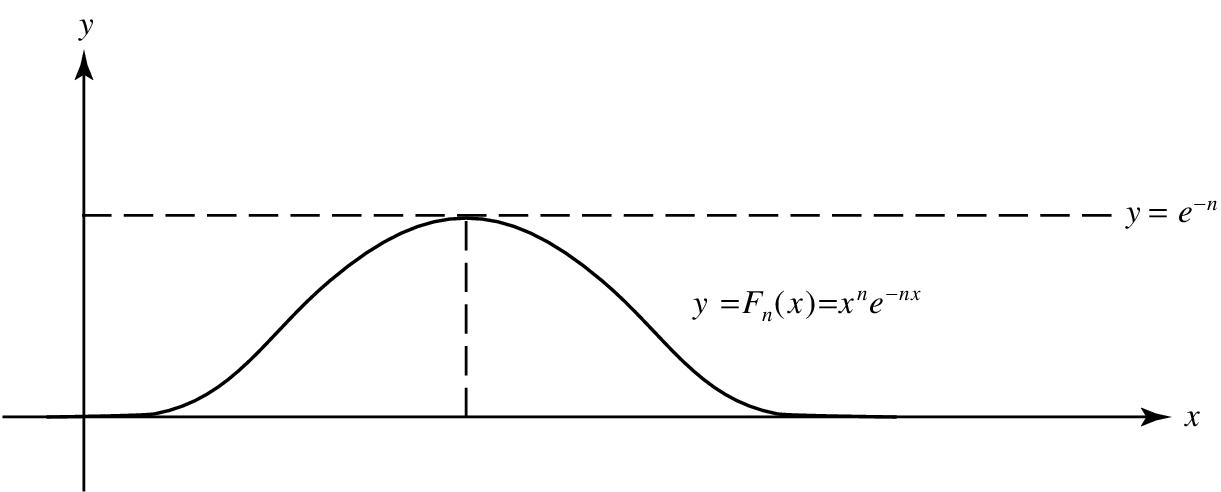
\includegraphics[width=4.1in,height=1.6in]{png/fig040401.png}
\end{center}
 \vskip6pt
 \refstepcounter{figure}
 \centerline{\bf Figure \thefigure} \label{figure:4.4.1}
 \vskip12pt



\noindent
 Equating the derivative
$$
F'_n(x)=nx^{n-1}e^{-nx}(1-x)
$$
 to zero shows that the maximum value of $F_n(x)$ on $[0,\infty)$ is
$e^{-n}$, attained at $x=1$.  Therefore,
$$
|F_n(x)|\le e^{-n},\quad x\ge0,
$$
 so $\lim_{n\to\infty} F_n(x)=0$ for all $x\ge0$.  The limit
function in this case is identically zero on $[0,\infty)$.
\end{example}


\begin{example}\label{example:4.4.3}\rm
For $n\ge1$, let $F_n$ be defined on
$(-\infty,\infty)$ by
$$
F_n(x)=\left\{\casespace\begin{array}{ll}
 0,&x<-\frac{2}{n},\\[3\jot]
-n(2+nx),&-\frac{2}{n}\le x<-\frac{1}{n},\\[3\jot]
 n^2x,&-\frac{1}{n}\le x<\frac{1}{n},\\[3\jot]
 n(2-nx),&\frac{1}{n}\le x<\frac{2}{n},\\[3\jot]
 0,&x\ge\frac{2}{n}\end{array}\right.
$$
(Figure~\ref{figure:4.4.2}, page~\pageref{figure:4.4.2}),
\vskip12pt
 Since $F_n(0)=0$ for all $n$,
 $\lim_{n\to \infty}F_n(0)=0$. If $x\ne0$, then $F_n(x)=0$ if
$n\ge2/|x|$. Therefore,
$$
\lim_{n\to\infty}F_n(x)=0,\quad-\infty<x<\infty,
$$
so the limit function is identically zero on $(-\infty,\infty)$.
\end{example}



\begin{example}\label{example:4.4.4}\rm  For each positive integer $n$,
let $S_n$ be the set of numbers of the form $x=p/q$, where $p$ and $q$
are  integers with no common factors and $1\le q\le n$. Define
$$
F_n(x)=\left\{\casespace\begin{array}{ll} 1,&x\in S_n,\\
0,&x\not\in S_n.\end{array}\right.
$$
\newpage
\noindent
If $x$ is irrational, then $x\not\in S_n$ for any $n$, so $F_n(x)=0$,
$n\ge 1$.
 If $x$ is rational, then $x\in S_n$ and
$F_n(x)=1$ for all sufficiently large $n$. Therefore,
$$
\lim_{n\to\infty} F_n(x)=F(x)=\left\{\casespace\begin{array}{ll} 1&\mbox{if $x$
is rational},\\
0&\mbox{if $x$ is irrational}.\end{array}\right.
$$
\end{example}

\begin{center}
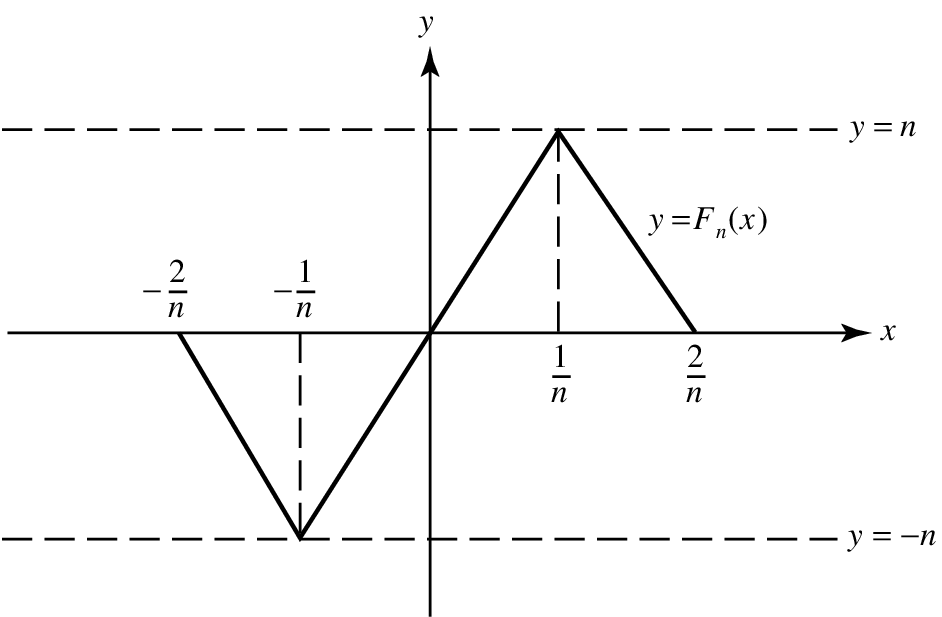
\includegraphics[width=3.15in,height=2.1in]{png/fig040402.png}
\end{center}
 \vskip10pt
 \refstepcounter{figure}
 \centerline{\bf Figure \thefigure} \label{figure:4.4.2}
 \vskip18pt

\boxit{Uniform Convergence}
\hskip-.4em
The pointwise limit of a sequence of functions may differ radically
from the functions in the sequence. In Example~\ref{example:4.4.1},
each $F_n$ is continuous on $(-\infty,1]$, but $F$ is not. In
Example~\ref{example:4.4.3}, the graph of each $F_n$ has two triangular
spikes with heights  that tend to $\infty$ as $n\to\infty$, while
the graph of
$F$
(the
$x$-axis) has none. In Example~\ref{example:4.4.4}, each $F_n$ is
integrable, while $F$ is nonintegrable on every finite
interval.
(Exercise~\ref{exer:4.4.3}). There is nothing in
Definition~\ref{thmtype:4.4.1}
to preclude these apparent anomalies; although the definition implies
that for each $x_0$ in $S$, $F_n(x_0)$ approximates $F(x_0)$ if $n$ is
sufficiently large, it does not imply that any particular $F_n$
approximates $F$ well over {\it all\/} of $S$. To formulate a definition
that does, it is convenient to introduce the notation
$$
\|g\|_S=\sup_{x\in S}|g(x)|
$$
and to state the following lemma. We leave the proof to you
(Exercise~\ref{exer:4.4.4}).


\begin{lemma} \label{thmtype:4.4.2}
If $g$ and $h$ are defined on $S,$ then
\begin{eqnarray*}
\|g+h\|_S\ar\le\|g\|_S+\|h\|_S\\
\arraytext{and}\\
\|gh\|_S\ar\le\|g\|_S\|h\|_S.
\end{eqnarray*}
Moroever$,$ if either $g$ or $h$ is bounded on $S,$ then
$$
\|g-h\|_S\ge\left|\|g\|_S-\|h\|_S\|\right|.
$$
\end{lemma}

\enlargethispage{1in}
\newpage


\begin{definition} \label{thmtype:4.4.3}
A sequence $\{F_n\}$ of functions defined on a set $S$
{\it converges uniformly to the limit function $F$ on\/} $S$ if
$$
\lim_{n\to\infty} || F_n-F\|_S=0.
$$
Thus, $\{F_n\}$ converges uniformly to $F$ on $S$ if for each
$\epsilon> 0$ there is an integer $N$ such that
\begin{equation} \label{eq:4.4.1}
\|F_n-F\|_S<\epsilon\mbox{\quad if\quad} n\ge N.
\end{equation}
\end{definition}
\vskip-1em\mbox{}\bbox\vskip1em

If $S=[a,b]$ and $F$ is the function with graph shown in
Figure~\ref{figure:4.4.3},
 then \eqref{eq:4.4.1} implies that the graph of
$$
y=F_n(x),\quad a\le x\le b,
$$
lies in the shaded band
$$
F(x)-\epsilon<y<F(x)+\epsilon,\quad a\le x\le b,
$$
if $n\ge N$.





From Definition~\ref{thmtype:4.4.3}, if $\{F_n\}$ converges uniformly on
$S$, then $\{F_n\}$ converges uniformly on any subset of $S$
(Exercise~\ref{exer:4.4.6}).

\vskip12pt
\begin{center}
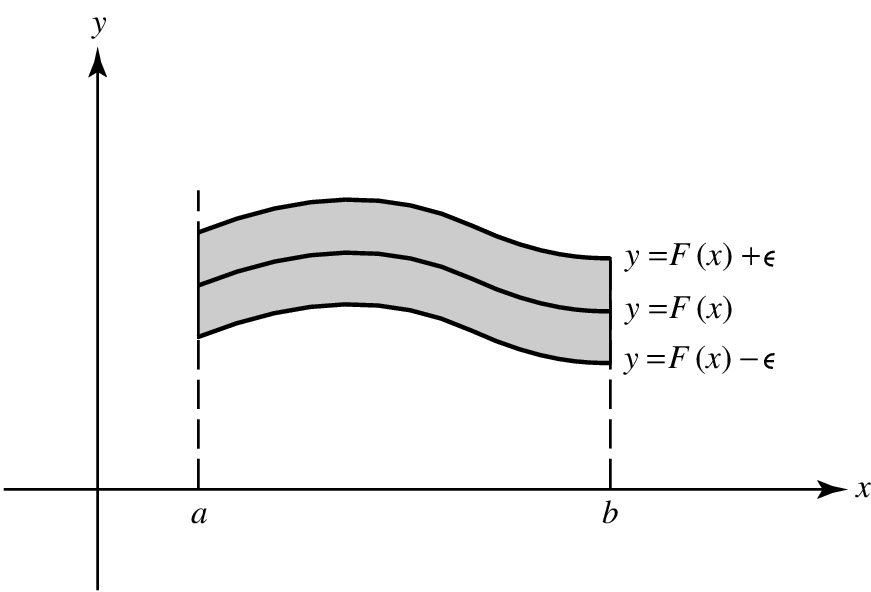
\includegraphics[width=3in,height=2in]{png/fig040403.png}
\end{center}
 \vskip6pt
 \refstepcounter{figure}
 \centerline{\bf Figure \thefigure} \label{figure:4.4.3}
 \vskip12pt

\begin{example}\label{example:4.4.5}\rm    The sequence $\{F_n\}$ defined by
$$
F_n(x)=x^ne^{-nx},\quad n\ge1,
$$
converges uniformly to $F\equiv0$ (that is, to the identically zero
function) on $S=[0,\infty)$, since we saw in Example~\ref{example:4.4.2}
that
$$
\|F_n-F\|_S=\|F_n\|_S=e^{-n},
$$
\newpage
\noindent
so
$$
\|F_n-F\|_S<\epsilon
$$
if $n>-\log\epsilon$.  For these values of $n$, the graph of
$$
y=F_n(x),\quad 0\le x<\infty,
$$
lies in the strip
$$
-\epsilon\le y\le\epsilon,\quad x\ge0
$$
(Figure~\ref{figure:4.4.4}).
\bbox\end{example}

The next theorem provides alternative definitions of pointwise and
uniform convergence.
It follows immediately from Definitions~\ref{thmtype:4.4.1}
and \ref{thmtype:4.4.3}.





\begin{theorem} \label{thmtype:4.4.4}
Let $\{F_n\}$ be defined on $S.$
Then
\begin{alist}
\item % (a)
$\{F_n\}$ converges pointwise to $F$ on $S$ if and only if there is,
for each $\epsilon>0$ and $x\in S$, an integer $N$ $($which may depend
on $x$ as well as $\epsilon)$ such that
$$
|F_n(x)-F(x)|<\epsilon\mbox{\quad if\quad}\ n\ge N.
$$
\item % (b)
 $\{F_n\}$ converges uniformly to $F$ on $S$ if and only if
there is for each $\epsilon>0$ an integer $N$ $($which depends only on
$\epsilon$ and not on any particular $x$ in $S)$ such that
$$
|F_n(x)-F(x)|<\epsilon\mbox{\quad for all $x$ in $S$ if $n\ge N$}.
$$
\end{alist}
\end{theorem}

 \vspace*{12pt}
\begin{center}
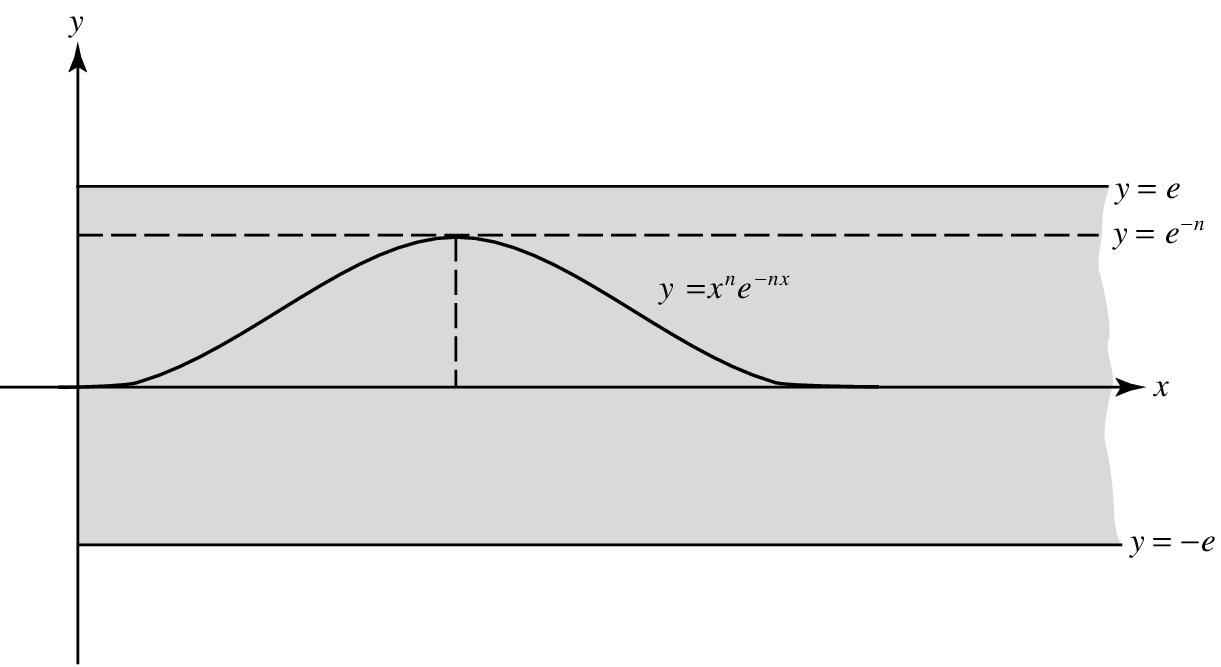
\includegraphics[width=4.1in,height=2.3in]{png/fig040404.png}
\end{center}
 \vskip6pt
 \refstepcounter{figure}
 \centerline{\bf Figure \thefigure} \label{figure:4.4.4}
 \vskip12pt

The next theorem follows immediately from Theorem~\ref{thmtype:4.4.4} and
Example~\ref{example:4.4.6}.



\begin{theorem} \label{thmtype:4.4.5}
If $\{F_n\}$ converges uniformly to $F$ on $S,$ then $\{F_n\}$ converges
pointwise to $F$ on $S.$ The converse is false$;$ that is$,$ pointwise
convergence does not imply uniform convergence.
\end{theorem}

\begin{example}\label{example:4.4.6}\rm  The sequence $\{F_n\}$ of
Example~\ref{example:4.4.3} converges pointwise to $F\equiv0$ on
$(-\infty,\infty)$, but not uniformly, since
$$
\|F_n-F\|_{(-\infty,\infty)}=F_n\left(\frac{1}{ n}\right)=\left|
F_n
\left(\frac{-1}{ n}\right)\right|=n,
$$
so
$$
\lim_{n\to\infty}\|F_n-F\|_{(-\infty,\infty)}=\infty.
$$
However, the convergence is uniform on
$$
S_\rho=(-\infty,\rho]\cup [\rho,\infty)
$$
for any $\rho>0$, since
$$
\|F_n-F\|_{S_\rho}=0\mbox{\quad if\quad} n>\frac{2}{\rho}.
$$
\end{example}

\begin{example}\label{example:4.4.7}\rm  If $F_n(x)=x^n$, $n\ge1$, then
$\{F_n\}$ converges pointwise on $S=[0,1]$ to
$$
F(x)=\left\{\casespace\begin{array}{ll} 1,&x=1,\\
0,&0\le x<1.\end{array}\right.
$$
The convergence is not uniform on $S$. To see this, suppose that
$0<\epsilon<1$. Then
$$
|F_n(x)-F(x)|>1-\epsilon
\mbox{\quad if \quad}
(1-\epsilon)^{1/n}<x<1.
$$
Therefore,
$$
1-\epsilon\le\|F_n-F\|_S\le1
$$
for all $n\ge1$. Since $\epsilon$ can be arbitrarily small, it follows
that
$$
\|F_n-F\|_S=1
$$
for all $n\ge1$.

 However, the convergence is uniform on $[0,\rho]$ if $0<
\rho<1$, since then
$$
\|F_n-F\|_{[0,\rho]}=\rho^n
$$
and $\lim_{n\to\infty}\rho^n=0$. Another way to say the same thing:
$\{F_n\}$ converges uniformly on every closed subset of $[0,1)$.
\bbox\end{example}

The next theorem enables us to test a sequence for uniform convergence
without guessing what the limit function might be. It is analogous to
Cauchy's convergence criterion for sequences of constants
(Theorem~\ref{thmtype:4.1.13}).


\begin{theorem} [Cauchy's Uniform Convergence
Criterion] \label{thmtype:4.4.6} \hspace*{-.5em}
A sequence of functions $\{F_n\}$ converges uniformly on a set $S$ if
and
only if for each $\epsilon>0$ there is an integer $N$ such that
\begin{equation} \label{eq:4.4.2}
\|F_n-F_m\|_S<\epsilon\mbox{\quad if\quad} n, m\ge N.
\end{equation}
\end{theorem}

\proof
For necessity, suppose that  $\{F_n\}$ converges uniformly to
$F$ on $S$. Then, if $\epsilon>0$, there is an integer $N$ such that
$$
\|F_k-F\|_S<\frac{\epsilon}{2}\mbox{\quad if\quad} k\ge N.
$$
Therefore,
\begin{eqnarray*}
\|F_n-F_m\|_S\ar=\|(F_n-F)+(F-F_m)\|_S\\
\ar\le \|F_n-F\|_S+\|F-F_m\|_S \mbox{\quad
(Lemma~\ref{thmtype:4.4.2})\quad}\\
&<&\frac{\epsilon}{2}+\frac{\epsilon}{2}=\epsilon\mbox{\quad if\quad}
m, n\ge N.
\end{eqnarray*}

For sufficiency, we first observe that \eqref{eq:4.4.2} implies that
$$
|F_n(x)-F_m(x)|<\epsilon\mbox{\quad if\quad} n, m\ge N,
$$
for any fixed $x$ in $S$. Therefore, Cauchy's convergence criterion
for sequences of constants (Theorem~\ref{thmtype:4.1.13})
implies that
$\{F_n(x)\}$ converges for each $x$ in $S$; that is, $\{F_n\}$
converges pointwise to a limit function $F$ on $S$. To see that the
convergence is uniform, we write
\begin{eqnarray*}
|F_m(x)-F(x) |\ar=|[F_m(x)-F_n(x)]+[F_n(x)-F(x)]|\\
\ar\le |F_m(x)-F_n(x)|+| F_n(x)-F(x)|\\
\ar\le \|F_m-F_n\|_S+|F_n(x)-F(x)|.
\end{eqnarray*}
This and \eqref{eq:4.4.2} imply that
\begin{equation} \label{eq:4.4.3}
|F_m(x)-F(x)|<\epsilon+|F_n(x)-F(x)|\quad\mbox {if}\quad n, m\ge N.
\end{equation}
Since $\lim_{n\to\infty}F_n(x)=F(x)$,
$$
|F_n(x)-F(x)|<\epsilon
$$
for some $n\ge N$, so \eqref{eq:4.4.3} implies that
$$
|F_m(x)-F(x)|<2\epsilon\mbox{\quad if\quad} m\ge N.
$$
But this inequality holds for all $x$ in $S$, so
$$
\|F_m-F\|_S\le2\epsilon\mbox{\quad if\quad} m\ge N.
$$
Since $\epsilon$ is an arbitrary positive number, this implies that
$\{F_n\}$ converges uniformly to $F$ on~$S$.
\bbox

The next example is similar to Example~\ref{example:4.1.14}.
\newpage

\begin{example}\label{example:4.4.8}\rm  Suppose that  $g$ is
differentiable on $S= (-\infty,\infty)$ and
\begin{equation} \label{eq:4.4.4}
|g'(x)|\le r<1,\quad-\infty<x<\infty.
\end{equation}
Let $F_0$ be bounded on $S$ and define
\begin{equation} \label{eq:4.4.5}
F_n(x)=g(F_{n-1}(x)),\quad n\ge1.
\end{equation}
We will show that $\{F_n\}$ converges uniformly on $S$.
We first note that if $u$ and $v$ are any two real numbers,
then \eqref{eq:4.4.4} and the mean value theorem imply that
\begin{equation} \label{eq:4.4.6}
|g(u)-g(v)|\le r|u-v|.
\end{equation}
Recalling \eqref{eq:4.4.5} and
applying this inequality with $u=F_{n-1}(x)$ and $v=0$ shows that
\begin{eqnarray*}
|F_n(x)|\ar=|g(0)+(g(F_{n-1}(x))-g(0))|\le|g(0)|+|g(F_{n-1}(x))-g(0)|\\
\ar\le |g(0)|+r|F_{n-1}(x)|;
\end{eqnarray*}
therefore, since $F_0$ is bounded on $S$,
it follows by induction that $F_n$ is bounded on $S$
for  $n\ge1$. Moreover, if $n\ge1$, then \eqref{eq:4.4.5} and
\eqref{eq:4.4.6} with $u=F_n(x)$ and $v=F_{n-1}(x)$ imply that
$$
|F_{n+1}(x)-F_n(x)|=|g(F_n(x))-g(F_{n-1}(x))| \le
r|F_n(x)-F_{n-1}(x)|,\quad-\infty<x<\infty,
$$ so
$$
\|F_{n+1}-F_n\|_S\le r\|F_n-F_{n-1}\|_S.
$$
By induction, this implies
that
\begin{equation} \label{eq:4.4.7}
\|F_{n+1}-F_n\|_S\le
r^n\|F_1-F_0\|_S.
\end{equation} If $n>m$, then
\begin{eqnarray*}
\|F_n-F_m\|_S\ar=\|(F_n-F_{n-1})+(F_{n-1}-F_{n-2})+\cdots+
(F_{m+1}-F_m)\|_S\\
\ar\le \|F_n-F_{n-1}\|_S+\|F_{n-1}-F_{n-2}\|_S+\cdots+
\|F_{m+1}-F_m\|_S,
\end{eqnarray*}
from Lemma~\ref{thmtype:4.4.2}. Now
\eqref{eq:4.4.7} implies that
\begin{eqnarray*}
\|F_n-F_m\|_S\ar\le \|F_1-F_0\|_S(1+r+r^2+\cdots+r^{n-m-1})r^m\\
&<&\|F_1-F_0\|_S \frac{r^m}{1-r}.
 \end{eqnarray*} Therefore, if
$$
\|F_1-F_0\|_S \frac{r^N}{1-r}<\epsilon,
$$
then $\|F_n-F_m\|_S<\epsilon$
if $n$, $m\ge N$. Therefore, $\{F_n\}$
converges uniformly on $S$, by Theorem~\ref{thmtype:4.4.6}.
\end{example}

\newpage

\boxit{Properties Preserved by Uniform Convergence}
We now study properties of the functions of a
uniformly convergent sequence that are inherited by the limit
function. We first consider continuity.


\begin{theorem} \label{thmtype:4.4.7}
If $\{F_n\}$ converges uniformly to $F$ on $S$ and each $F_n$ is
continuous at a point $x_0$ in $S,$ then so is $F$. Similar
statements hold for continuity from the right and left$.$
\end{theorem}

\proof
Suppose that  each $F_n$ is continuous at $x_0$.
If $x\in S$ and $n\ge1$, then
\begin{equation} \label{eq:4.4.8}
\begin{array}{rcl}
|F(x)-F(x_0)|\ar\le  |F(x)-F_n(x)|+|F_n(x)-F_n(x_0)|+|F_n(x_0)-F(x_0)|
\\
\ar\le  |F_n(x)-F_n(x_0)|+2\|F_n-F\|_S.
\end{array}
\end{equation}
Suppose that  $\epsilon>0$. Since $\{F_n\}$ converges uniformly to $F$
on $S$, we can choose $n$ so that $\|F_n-F\|_S<\epsilon$. For this
fixed  $n$, \eqref{eq:4.4.8} implies that
\begin{equation} \label{eq:4.4.9}
|F(x)-F(x_0)|<|F_n(x)-F_n(x_0)|+2\epsilon,\quad x\in S.
\end{equation}
Since $F_n$ is continuous at $x_0$, there is a $\delta>0$ such that
$$
|F_n(x)-F_n(x_0)|<\epsilon\mbox{\quad if\quad} |x-x_0|<\delta,
$$
so, from \eqref{eq:4.4.9},
$$
|F(x)-F(x_0)|<3\epsilon,\mbox{\quad if\quad} |x-x_0|<\delta.
$$
Therefore, $F$ is continuous at $x_0$. Similar
arguments apply to the assertions on
continuity from the right and left.
\bbox

\enlargethispage{.5\baselineskip}

\begin{corollary} \label{thmtype:4.4.8}
If $\{F_n\}$ converges uniformly to $F$ on $S$ and each $F_n$ is
continuous on $S,$ then so is $F;$ that is$,$ a uniform limit of
continuous functions is continuous.
\end{corollary}

Now we consider the question of integrability of the uniform limit of
integrable functions.


\begin{theorem} \label{thmtype:4.4.9}
Suppose that  $\{F_n\}$ converges uniformly to $F$ on $S=[a,b]$. Assume
that $F$ and all $F_n$
are   integrable on $[a,b].$ Then
\begin{equation} \label{eq:4.4.10}
\int_a^b F(x)\,dx=\lim_{n\to\infty}\int_a^b F_n(x)\,dx.
\end{equation}
\end{theorem}

\proof  Since
\begin{eqnarray*}
\left|\int_a^b F_n(x)\,dx-\int_a^b F(x)\,dx\right|\ar\le \int_a^b
|F_n(x)-F(x)|\,dx\\
\ar\le  (b-a)\|F_n-F\|_S
\end{eqnarray*}
and $\lim_{n\to\infty}\|F_n-F\|_S=0$, the conclusion follows.
\bbox

In particular, this theorem implies that \eqref{eq:4.4.10} holds if each
$F_n$ is continuous on $[a,b]$, because then $F$ is continuous
(Corollary~\ref{thmtype:4.4.8}) and therefore integrable on $[a,b]$.

The hypotheses of Theorem~\ref{thmtype:4.4.9} are stronger than necessary.
We state the next theorem so that  you will be better informed on this
subject. We omit the proof, which  is inaccessible if you
skipped Section~3.5, and quite involved in any case.

\begin{theorem} \label{thmtype:4.4.10}
 Suppose that  $\{F_n\}$ converges
pointwise to $F$ and each $F_n$ is integrable on $[a,b].$
\begin{alist}
\item % (a)
If the convergence is uniform$,$ then $F$ is integrable on
$[a,b]$ and $\eqref{eq:4.4.10}$ holds.
\item % (b)
If the sequence $\{\|F_n\|_{[a,b]}\}$ is bounded and $F$ is
integrable on $[a,b],$ then $\eqref{eq:4.4.10}$ holds.
\end{alist}
\end{theorem}

Part \part{a} of this theorem shows that it is not necessary to assume in
Theorem~\ref{thmtype:4.4.9} that $F$ is integrable on $[a,b]$, since this
follows from the uniform convergence. Part \part{b} is known as the {\it
bounded convergence theorem}.
Neither of the assumptions of
\part{b}
 can
be omitted. Thus, in Example~\ref{example:4.4.3}, where
$\{\|F_n\|_{[0,1]}\}$ is unbounded while $F$ is integrable on $[0,1]$,
$$
\int^1_0 F_n(x)\,dx=1,\quad n\ge1,\mbox{\quad but\quad}
\int^1_0 F(x)\,dx=0.
$$
In Example~\ref{example:4.4.4}, where $\|F_n\|_{[a,b]}=1$ for every
finite
interval $[a,b]$, $F_n$ is integrable for all $n\ge1$, and $F$ is
nonintegrable on every interval (Exercise~\ref{exer:4.4.3}).

After Theorems~\ref{thmtype:4.4.7} and \ref{thmtype:4.4.9}, it may seem
reasonable to expect that if a sequence $\{F_n\}$ of differentiable
functions converges uniformly to $F$ on $S$, then
$F'=\lim_{n\to\infty}F'_n$ on $S$. The next example shows that this
is not true in general.

\begin{example}\label{example:4.4.9}\rm  The sequence $\{F_n\}$ defined by
$$
F_n(x)=x^n\sin \frac{1}{ x^{n-1}}
$$
converges uniformly to $F\equiv0$ on $[r_1,r_2]$ if $0<r_1<r_2<1$
(or, equivalently, on every compact subset of $(0,1)$).  However,
$$
F'_n(x)=nx^{n-1}\sin\frac{1}{ x^{n-1}}-(n-1)\cos \frac{1}{ x^{n-1}},
$$
so $\{F'_n(x)\}$ does not converge for any $x$ in $(0,1)$.
\end{example}


\begin{theorem} \label{thmtype:4.4.11}
Suppose that  $F'_n$ is continuous on $[a,b]$ for all $n\ge1$ and $\{F'_n\}$
converges uniformly on $[a,b].$ Suppose also that
 $\{F_n(x_0)\}$ converges for some $x_0$ in $[a,b].$ Then
$\{F_n\}$ converges uniformly on $[a,b]$ to a differentiable limit
function $F,$ and
\begin{equation} \label{eq:4.4.11}
F'(x)=\lim_{n\to\infty}F'_n(x),\quad a<x<b,
\end{equation}
while
\begin{equation} \label{eq:4.4.12}
F'_+(a)=\lim_{n\to\infty}F'_n(a+)\mbox{\quad and\quad} F'_-(b)=
\lim_{n\to\infty}F'_n(b-).
\end{equation}
\end{theorem}
\newpage

\proof
 Since $F'_n$ is continuous on $[a,b]$, we can write
\begin{equation} \label{eq:4.4.13}
F_n(x)=F_n(x_0)+\int^x_{x_0} F'_n(t)\,dt,\quad a\le x\le b
\end{equation}
 (Theorem~\ref{thmtype:3.3.12}).  Now let
\begin{eqnarray}
L\ar=\lim_{n\to\infty}F_n(x_0)\nonumber\\
\arraytext{and}\nonumber\\
G(x)\ar=\lim_{n\to\infty} F'_n(x).\label{eq:4.4.14}
\end{eqnarray}
Since $F'_n$ is continuous and $\{F'_n\}$ converges uniformly to $G$
on $[a,b]$, $G$ is continuous on $[a,b]$ (Corollary~\ref{thmtype:4.4.8});
therefore, \eqref{eq:4.4.13} and
Theorem~\ref{thmtype:4.4.9} (with $F$ and $F_n$ replaced by $G$ and
$F_n'$) imply that
$\{F_n\}$ converges pointwise on
$[a,b]$ to the limit function
\begin{equation} \label{eq:4.4.15}
F(x)=L+\int^x_{x_0} G(t)\,dt.
\end{equation}
 The convergence is actually uniform on $[a,b]$, since
subtracting
\eqref{eq:4.4.13} from \eqref{eq:4.4.15} yields
\begin{eqnarray*}
|F(x)-F_n(x)|\ar\le |L-F_n(x_0)|+\left|\int_{x_0}^x|G(t)-F_n'(t)|\,dt\right|\\
\ar\le |L-F_n(x_0)|+|x-x_0|\,\|G-F_n'\|_{[a,b]},
\end{eqnarray*}
so
$$
\|F-F_n\|_{[a,b]}\le|L-F_n(x_0)|+(b-a)\|G-F'_n\|_{[a,b]},
$$
where the right side approaches zero as $n\to\infty$.

Since $G$ is continuous on $[a,b]$, \eqref{eq:4.4.14}, \eqref{eq:4.4.15},
Definition~\ref{thmtype:2.3.6}, and
Theorem~\ref{thmtype:3.3.11} imply \eqref{eq:4.4.11}
and \eqref{eq:4.4.12}.
\bbox

\boxit{Infinite Series of Functions}
In Section~4.3\ we defined the sum of an infinite series of
constants as the limit of the sequence of partial sums. The same
definition can be applied to series of functions, as follows.


\enlargethispage{100pt}
\begin{definition} \label{thmtype:4.4.12}
If $\{f_j\}^\infty_k$ is a sequence of real-valued functions defined
on a set $D$ of reals, then $\sum_{j=k}^\infty  f_j$ is  an
{\it infinite series\/} (or simply a {\it
series\/}) of functions on
$D$. The {\it partial sums of\/},
$\sum_{j=k}^\infty f_j$ are defined by
$$
F_n=\sum^n_{j=k} f_j,\quad n\ge k.
$$
If $\{F_n\}^\infty_k$ converges pointwise to a function $F$ on a
subset $S$ of $D$, we say that $\sum_{j=k}^\infty f_j$ {\it converges
pointwise to the sum $F$ on\/} $S$, and write
$$
F=\sum_{j=k}^\infty f_j,\quad x\in S.
$$
\newpage
\noindent
If $\{F_n\}$ converges uniformly to $F$ on $S$, we say that
$\sum_{j=k}^\infty f_j$ {\it converges uniformly to $F$ on~$S$\/}.
\end{definition}

\begin{example}\label{example:4.4.10}\rm
The functions
$$
f_j(x)=x^j,\quad j\ge0,
$$
define the infinite series
$$
\sum_{j=0}^\infty x^j
$$
on $D=(-\infty,\infty)$.  The  $n$th partial sum of the series is
$$
F_n(x)=1+x+x^2+\cdots+x^n,
$$
 or, in closed form,
$$
F_n(x)=\left\{\casespace\begin{array}{ll}
\dst{\frac{1-x^{n+1}}{1-x}},&x\ne1,\\[2\jot]
 n+1,&x=1\end{array}\right.
$$
(Example~\ref{example:4.1.11}). We have seen earlier that
$\{F_n\}$ converges pointwise to
$$
F(x)=\frac{1}{1-x}
$$
if $|x|<1$ and diverges if $|x|\ge1$; hence, we write
$$
\sum_{j=0}^\infty x^j=\frac{1}{1-x},\quad-1<x<1.
$$

Since the difference
$$
F(x)-F_n(x)=\frac{x^{n+1}}{1-x}
$$
can be made arbitrarily large by taking $x$ close to $1$,
$$
\|F-F_n\|_{(-1,1)}=\infty,
$$
so the convergence is not uniform on $(-1,1)$.  Neither is it uniform
on any interval $(-1,r]$ with $-1<r<1$, since
$$
\|F-F_n\|_{(-1,r)}\ge\frac{1}{2}
$$
for every $n$ on every such interval.  (Why?)  The series does converge
uniformly on any interval $[-r,r]$ with $0<r<1$, since
$$
\|F-F_n\|_{[-r,r]}=\frac{r^{n+1}}{1-r}
$$
and $\lim_{n\to\infty}r^n=0$.  Put another way, the series converges
uniformly on closed subsets of $(-1,1)$.
\bbox\end{example}

\newpage

As for series of constants, the convergence, pointwise or
uniform, of a series of functions is not changed by altering or
omitting finitely many terms. This justifies adopting the convention
that we used for series of constants: when we are interested only in
whether
a series of functions converges, and not in its sum, we will omit the
limits on the summation sign and write simply $\sum f_n$.

\boxit{Tests for Uniform Convergence of Series}
Theorem~\ref{thmtype:4.4.6} is easily converted to a theorem on uniform
convergence of series, as follows.


\begin{theorem} [Cauchy's  Uniform Convergence Criterion]
\label{thmtype:4.4.13}
A series $\sum f_n$ converges uniformly on a set $S$ if and only if
for each $\epsilon>0$ there is an integer $N$ such that
\vskip0pt
\begin{equation} \label{eq:4.4.16}
\|f_n+f_{n+1}+\cdots+f_m\|_S<\epsilon\mbox{\quad if\quad} m\ge n\ge
N.
\end{equation}
\end{theorem}
\vskip5pt
\proof
 Apply Theorem~\ref{thmtype:4.4.6} to the partial sums of
$\sum f_n$, observing that
$$
f_n+f_{n+1}+\cdots+f_m=F_m-F_{n-1}.
$$
\vskip-2em\bbox\vskip2em


Setting $m=n$ in \eqref{eq:4.4.16} yields the
following necessary, but  not
sufficient, condition for uniform convergence of series. It is
analogous to Corollary~\ref{thmtype:4.3.6}.

\vskip5pt

\begin{corollary} \label{thmtype:4.4.14}
If $\sum f_n$ converges uniformly on $S,$ then
$\lim_{n\to\infty}\|f_n\|_S=0.$
\end{corollary}

Theorem~\ref{thmtype:4.4.13} leads immediately to the following important
test for uniform convergence of series.

\vskip5pt

\begin{theorem} [Weierstrass's Test] \label{thmtype:4.4.15}
The series $\sum f_n$ converges uniformly on $S$ if
\begin{equation} \label{eq:4.4.17}
\|f_n\|_S\le M_n,\quad n\ge k,
\end{equation}
where $\sum M_n<\infty.$
\end{theorem}

\vskip5pt

\proof
From Cauchy's convergence criterion for series of constants,
there is for each $\epsilon>0$ an integer $N$ such that
$$
M_n+M_{n+1}+\cdots+M_m<\epsilon\mbox{\quad if\quad} m\ge n\ge N,
$$
which, because of \eqref{eq:4.4.17}, implies that
$$
\|f_n\|_S+\|f_{n+1}\|_S+\cdots+\|f_m\|_S<\epsilon\mbox{\quad if\quad}
 m, n\ge N.
$$
 Lemma~\ref{thmtype:4.4.2} and Theorem~\ref{thmtype:4.4.13} imply that
$\sum f_n$ converges uniformly on $S$.
\mbox{}\bbox


\begin{example}\label{example:4.4.11}\rm  Taking $M_n=1/n^2$ and recalling
that
$$
\sum \frac{1}{ n^2}<\infty,
$$
we see that
$$
\sum \frac{1}{ x^2+n^2}\mbox{\quad and\quad}\sum\frac{\sin nx}{ n^2}
$$
converge uniformly on $(-\infty,\infty)$.
\end{example}

\begin{example}\label{example:4.4.12}\rm    The series
$$
\sum f_n(x)=\sum\left(\frac{x}{1+x}\right)^n
$$
converges uniformly on any set $S$ such that
\begin{equation} \label{eq:4.4.18}
\left|\frac{x}{1+x}\right|\le r<1,\quad x\in S,
\end{equation}
because if $S$ is such a set, then
$$
\|f_n\|_S\le r^n
$$
and Weierstrass's test applies, with
$$
\sum M_n=\sum r^n<\infty.
$$
Since \eqref{eq:4.4.18} is equivalent to
$$
\frac{-r}{1+r}\le x\le \frac{r}{1-r},\quad x\in S,
$$
this means that the series converges uniformly on any compact subset
of $(-1/2,\infty)$. (Why?) From  Corollary~\ref{thmtype:4.4.14},
the series  does not converge uniformly on $S=(-1/2,b)$ with
$b<\infty$ or on $S=[a,\infty)$ with $a>-1/2$, because in these
cases $\|f_n\|_S= 1$ for all $n$.
\bbox\end{example}

Weierstrass's test is very important, but applicable only to series
that actually exhibit a stronger kind of convergence than we have
considered so far. We say that $\sum f_n$ {\it converges absolutely
on} $S$ if $\sum
|f_n|$ converges pointwise on
$S$, and
{\it
absolutely uniformly} on $S$ if
$\sum
|f_n|$ converges uniformly on
$S$. We leave it to you (Exercise~\ref{exer:4.4.21}) to verify that
our proof of Weierstrass's test actually shows that $\sum f_n$
converges absolutely uniformly on $S$. We also leave it to you  to
show that if a series
converges absolutely uniformly on $S$, then it converges uniformly
on $S$ (Exercise~\ref{exer:4.4.20}).

The next theorem applies to series that converge uniformly, but
perhaps not absolutely uniformly, on a set $S$.


\begin{theorem} [Dirichlet's Test for Uniform Convergence]
\label{thmtype:4.4.16}
The series
$$
\sum_{n=k}^\infty  f_ng_n
$$
 converges uniformly on
$S$ if
 $\{f_n\}$ converges uniformly to zero on $S,$
 $\sum (f_{n+1}-f_n)$ converges absolutely uniformly on
$S,$ and
\begin{equation} \label{eq:4.4.19}
\|g_k+g_{k+1}+\cdots+g_n\|_S\le M,\quad n\ge k,
\end{equation}
for some constant $M.$
\end{theorem}

\proof
The proof is similar to the proof of
Theorem~\ref{thmtype:4.3.20}. Let
$$
G_n=g_k+g_{k+1}+\cdots+g_n,
$$
and consider the partial sums of $\sum_{n=k}^\infty  f_ng_n$:
\begin{equation} \label{eq:4.4.20}
H_n=f_kg_k+f_{k+1}g_{k+1}+\cdots+f_ng_n.
\end{equation}
By substituting
$$
g_k=G_k\mbox{\quad and\quad} g_n=G_n-G_{n-1},\quad n\ge k+1,
$$
into \eqref{eq:4.4.20}, we obtain
$$
H_n=f_kG_k+f_{k+1}(G_{k+1}-G_k)+\cdots+f_n(G_n-G_{n-1}),
$$
which we rewrite as
$$
H_n=(f_k-f_{k+1})
G_k+(f_{k+1}-f_{k+2})G_{k+1}+\cdots+(f_{n-1}-f_n)G_{n-1}+f_nG_n,
$$
or
\begin{equation} \label{eq:4.4.21}
H_n=J_{n-1}+f_nG_n,
\end{equation}
where
\begin{equation} \label{eq:4.4.22}
J_{n-1}=(f_k-f_{k+1})G_k+(f_{k+1}-f_{k+2})
G_{k+1}+\cdots+(f_{n-1}-f_n)G_{n-1}.
\end{equation}
That is, $\{J_n\}$ is the sequence of partial sums of the series
\begin{equation} \label{eq:4.4.23}
\sum_{j=k}^\infty (f_j-f_{j+1})G_j.
\end{equation}

 From \eqref{eq:4.4.19} and the definition of
$G_j$,
$$
\left|\sum^m_{j=n}[f_j(x)-f_{j+1}(x)]G_j(x)\right|\le M
\sum^m_{j=n}|f_j(x)-f_{j+1}(x)|,\quad x\in S,
$$
\newpage
\noindent so
$$
\left\|\sum^m_{j=n} (f_j-f_{j+1})G_j\right\|_S\le M\left\|\sum^m_{j=n}
|f_j-f_{j+1}|\right\|_S.
$$
Now suppose that   $\epsilon>0$.
Since $\sum (f_j-f_{j+1})$ converges absolutely uniformly on $S$,
Theorem~\ref{thmtype:4.4.13} implies that
there is an integer $N$ such that
the right side of the last
inequality is less than $\epsilon$ if
$m\ge n\ge N$. The same is then true of the left side, so
Theorem~\ref{thmtype:4.4.13}
 implies that
\eqref{eq:4.4.23} converges uniformly on~$S$.


We have now shown that $\{J_n\}$ as defined in \eqref{eq:4.4.22} converges
uniformly to a limit function $J$ on $S$. Returning to \eqref{eq:4.4.21},
we see that
$$
H_n-J=J_{n-1}-J+f_nG_n.
$$
Hence, from Lemma~\ref{thmtype:4.4.2} and \eqref{eq:4.4.19},
\begin{eqnarray*}
\|H_n-J\|_S\ar\le \|J_{n-1}-J\|_S+\|f_n\|_S\|G_n\|_S\\
\ar\le \|J_{n-1}-J\|_S+M\|f_n\|_S.
\end{eqnarray*}
Since $\{J_{n-1}-J\}$ and $\{f_n\}$ converge uniformly to zero on $S$,
it now follows that $\lim_{n\to\infty}\|H_n-J\|_S=0$. Therefore,
 $\{H_n\}$ converges uniformly on~$S$.
\bbox

\vspace*{5pt}

\begin{corollary} \label{thmtype:4.4.17}
The series $\sum_{n=k}^\infty  f_ng_n$ converges uniformly on $S$ if
$$
f_{n+1}(x)\le f_n(x),\quad x\in S,\quad n\ge k,
$$
$\{f_n\}$ converges uniformly to zero on $S,$ and
$$
\|g_k+g_{k+1}+\cdots+g_n\|_S\le M,\quad n\ge k,
$$
for some constant $M.$
\end{corollary}


The proof is similar to that of
Corollary~\ref{thmtype:4.3.21}. We leave it to you
(Exercise~\ref{exer:4.4.22}).

\vspace*{5pt}

\begin{example}\label{example:4.4.13}\rm    Consider the series
$$
\sum_{n=1}^\infty \frac{\sin nx}{ n}
$$
with $f_n=1/n$ (constant), $g_n(x)=\sin nx$, and
$$
G_n(x)=\sin x+\sin2x+\cdots+\sin nx.
$$
We saw in Example~\ref{example:4.3.21} that
$$
|G_n(x)|\le \frac{1}{ |\sin(x/2)|},\quad n\ge1,\quad n\ne2k\pi \quad
\mbox{\quad ($k=$ integer)}.
$$
\newpage
\noindent
Therefore, $\{\|G_n\|_S\}$ is bounded, and the series converges
uniformly on any set $S$ on which $\sin x/2$ is bounded away from
zero. For example, if $0<\delta<\pi$, then
$$
\left|\sin \frac{x}{2}\right|\ge\sin \frac{\delta}{2}
$$
if $x$ is at least $\delta$ away from any multiple of $2\pi$; hence,
the series converges uniformly on
$$
S=\bigcup^\infty_{k=-\infty}[2k\pi+\delta, 2(k+1)\pi-\delta].
$$
Since
$$
\sum\left|\frac{\sin nx}{ n}\right|=\infty,\quad x\ne k\pi
$$
(Exercise~\ref{exer:4.3.32}\part{b}), this result
cannot be obtained from Weierstrass's test.
\end{example}

\begin{example}\label{example:4.4.14}\rm    The series
$$
\sum_{n=1}^\infty \frac{(-1)^n}{ n+x^2}
$$
satisfies the hypotheses of Corollary~\ref{thmtype:4.4.17} on
$(-\infty,\infty)$, with
$$
f_n(x)=\frac{1}{ n+x^2},\quad g_n=(-1)^n,\quad G_{2m}=0,\quad
\mbox{\quad and\quad}\quad G_{2m+1}=-1.
$$
Therefore, the series  converges uniformly on $(-\infty,\infty)$.
This result cannot be obtained by Weierstrass's test, since
$$
\sum \frac{1}{ n+x^2}=\infty
$$
for all $x$.
\end{example}

\boxit{Continuity, Differentiability, and Integrability of Series}
We can obtain results on the continuity, differentiability, and
integrability of infinite series by applying Theorems~\ref{thmtype:4.4.7},
\ref{thmtype:4.4.9}, and \ref{thmtype:4.4.11} to their partial sums. We will
state the theorems and give some examples, leaving the proofs to
you.

Theorem~\ref{thmtype:4.4.7}  implies the following theorem
(Exercise~\ref{exer:4.4.23}).


\begin{theorem} \label{thmtype:4.4.18}
If $\sum_{n=k}^\infty  f_n$ converges uniformly to $F$ on $S$ and each
$f_n$ is continuous at a point $x_0$ in $S,$ then so is $F.$ Similar
statements hold for continuity from the right and left$.$
\end{theorem}


\begin{example}\label{example:4.4.15}\rm  In Example~\ref{example:4.4.12} we
saw that the series
$$
F(x)=\sum_{n=0}^\infty \left(\frac{x}{1+x}\right)^n
$$
\newpage
\noindent
converges uniformly on every compact subset of $(-1/2,
\infty)$. Since the terms of the series are continuous on every such
subset, Theorem~\ref{thmtype:4.4.4} implies that $F$ is also. In fact, we
can state a stronger result: $F$ is continuous on
$(-1/2,\infty)$, since every point in
$(-1/2,\infty)$ lies in a compact subinterval of
$(-1/2,\infty)$.

The same argument and the results of Example~\ref{example:4.4.13} show
that the function
$$
G(x)=\sum_{n=1}^\infty\frac{\sin nx}{ n}
$$
is continuous except perhaps at $x_k=2k\pi$ ($k=$ integer).

From Example~\ref{example:4.4.14}, the function
$$
H(x)=\sum_{n=1}^\infty  (-1)^n\frac{1}{ n+x^2}
$$
is continuous for all $x$.
\bbox\end{example}

The next theorem gives conditions that permit the interchange of
summation and integration of infinite series. It follows from
Theorem~\ref{thmtype:4.4.9} (Exercise~\ref{exer:4.4.25}). We leave it to you
to formulate an analog
of Theorem~\ref{thmtype:4.4.10} for series (Exercise~\ref{exer:4.4.26}).


\begin{theorem} \label{thmtype:4.4.19}
Suppose that  $\sum_{n=k}^\infty f_n$ converges uniformly to $F$ on
$S=[a,b].$ Assume that $F$ and  $f_n,$ $n\ge k,$
are   integrable on $[a,b].$ Then
$$
\int_a^b F(x)\,dx=\sum_{n=k}^\infty \int_a^b f_n(x)\,dx.
$$
\end{theorem}

We say in this case that $\sum_{n=k}^\infty f_n$ can be integrated {\it
term by term\/} over $[a,b]$.

\begin{example}\label{example:4.4.16}\rm    From Example~\ref{example:4.4.10},
$$
\frac{1}{1-x}=\sum_{n=0}^\infty  x^n,\quad-1<x<1.
$$
The series converges uniformly, and the limit function is
integrable on any closed subinterval $[a,b]$ of $(-1,1)$; hence,
$$
\int_a^b \frac{dx}{1-x}=\sum_{n=0}^\infty \int_a^b x^n\,dx,
$$
so
$$
\log (1-a)-\log(1-b)=\sum_{n=0}^\infty\frac{b^{n+1}-a^{n+1}}{ n+1}.
$$
Letting $a=0$ and $b=x$ yields
$$
\log(1-x)=-\sum_{n=0}^\infty\frac{x^{n+1}}{ n+1},\quad-1<x<1.
\eqno{\bbox}
$$
\end{example}

\newpage

The next theorem gives conditions that permit the interchange of
summation and differentiation of infinite series.
It follows from Theorem~\ref{thmtype:4.4.11} (Exercise~\ref{exer:4.4.28}).


\begin{theorem} \label{thmtype:4.4.20}
Suppose that  $f_n$ is continuously differentiable on $[a,b]$ for each
$n\ge k,$ $\sum_{n=k}^\infty f_n(x_0)$ converges for some $x_0$ in
$[a,b],$ and
$\sum_{n=k}^\infty  f'_n$ converges uniformly on $[a,b].$ Then
$\sum_{n=k}^\infty f_n$ converges uniformly on $[a,b]$ to a
differentiable function $F,$ and
$$
F'(x)=\sum_{n=k}^\infty  f'_n(x),\quad a<x<b,
$$
while
$$
F'(a+)=\sum_{n=k}^\infty  f'_n(a+)\mbox{\quad and\quad} F'(b-)=
\sum_{n=k}^\infty  f'_n(b-).
$$
\end{theorem}

We say in this case that $\sum_{n=k}^\infty f_n$ can be differentiated
{\it term by term\/}
 on $[a,b]$.
To apply Theorem~\ref{thmtype:4.4.20},
we first verify that $\sum_{n=k}^\infty f_n(x_0)$ converges for some
$x_0$  in $[a,b]$ and then differentiate $\sum_{n=k}^\infty f_n$
term by term. If the resulting series converges uniformly, then
term by term differentiation was legitimate.

\begin{example} \label{example:4.4.17}\rm
The series
\begin{equation} \label{eq:4.4.24}
\sum_{n=1}^\infty  (-1)^n\frac{1}{ n}\cos \frac{x}{ n}
\end{equation}
converges at $x_0=0$. Differentiating term by term yields
the series
\begin{equation} \label{eq:4.4.25}
\sum_{n=1}^\infty  (-1)^{n+1}\frac{1}{ n^2}\sin \frac{x}{ n}
\end{equation}
of continuous functions. This series  converges
 uniformly on $(-\infty,\infty)$, by Weierstrass's test.
By Theorem~\ref{thmtype:4.4.20}, the series  \eqref{eq:4.4.24} converges
uniformly on every finite interval to the differentiable function
\begin{eqnarray*}
F(x)\ar=
\sum_{n=1}^\infty  (-1)^n\frac{1}{ n}\cos \frac{x}{ n},\quad
-\infty<x<\infty,\\
\arraytext{and}\\
F'(x)\ar=
\sum_{n=1}^\infty  (-1)^{n+1}\frac{1}{ n^2}\sin \frac{x}{ n},\quad
-\infty<x<\infty.
\end{eqnarray*}
\end{example}

\begin{example}\label{example:4.4.18}\rm    The series
\begin{equation} \label{eq:4.4.26}
E(x)=\sum_{n=0}^\infty \frac{x^n}{
n!}=1+x+\frac{x^2}{2!}+\frac{x^3}{
3!}+\cdots
\end{equation}
\newpage

\noindent
converges uniformly on every interval $[-r,r]$ by Weierstrass's test,
because
\begin{eqnarray*}
\frac{|x|^n}{ n!}\ar\le \frac{r^n}{ n!},\quad |x|\le r,\\
\arraytext{and}\\
\sum\frac{r^n}{ n!}\ar<\infty
\end{eqnarray*}
for all $r$, by the ratio test. Differentiating the right side of
\eqref{eq:4.4.26} term by term yields the series
$$
\sum_{n=1}^\infty \frac{x^{n-1}}{(n-1)!}=\sum_{n=0}^\infty \frac{x^n}{ n!},
$$
which is the same as \eqref{eq:4.4.26}. Therefore, the differentiated
series is also uniformly convergent on $[-r,r]$ for every $r$, so
the term by term differentiation is legitimate and
$$
E'(x)=E(x),\quad-\infty<x<\infty.
$$
This is not surprising  if you recognize that $E(x)=e^x$.
\end{example}

\begin{example}\label{example:4.4.19}\rm  Failure to verify that the given
series converges at some point can lead to erroneous conclusions. For
example, differentiating \begin{equation} \label{eq:4.4.27}
\sum_{n=1}^\infty \cos\frac{x}{ n} \end{equation} term by term yields
$$
-\sum_{n=1}^\infty \frac{1}{ n}\sin \frac{x}{ n},
$$
which converges uniformly on $[-r,r]$ for every $r$, since
\begin{eqnarray*}
\left|\frac{1}{ n}\sin \frac{x}{ n}\right|\ar\le  \frac{|x|}{ n^2}
\mbox{\quad (Exercise~\ref{exer:2.3.19})\quad}\\
\ar\le  \frac{r}{ n^2} \mbox{\quad if \quad} |x|\le r,
\end{eqnarray*}
and $\sum 1/n^2<\infty$. We cannot conclude from this that
\eqref{eq:4.4.27} converges uniformly on $[-r,r]$. In fact, it diverges
for every $x$. (Why?)
\end{example}

\exercises
\begin{exerciselist}



\item\label{exer:4.4.1} Find the set $S$ on which $\{F_n\}$ converges
pointwise, and find the limit function.


\begin{tabular}[t]{@{}p{168pt}@{}p{168pt}}
 \part{a} $F_n(x)=x^n(1-x^2)$&\part{b} $F_n(x)=nx^n(1-x^2)$
\end{tabular}

\newpage

\begin{tabular}[t]{@{}p{168pt}@{}p{168pt}}
 \part{c} $F_n(x)=x^n(1-x^n)$&\part{d} $\dst{F_n(x)=\sin
\left(1+\frac{1}{ n}\right)x}$\\[2\jot]
 \part{e} $\dst{F_n(x)=\frac{1+x^n}{1+x^{2n}}}$&\part{f}
$\dst{F_n(x)=n\sin\frac{x}{ n}}$\\[2\jot]
 \part{g} $\dst{F_n(x)=n^2\left(1-\cos \frac{x}{
n}\right)}$&\part{h} $F_n(x)=nxe^{-nx^2}$\\[2\jot]
 \part{i} $\dst{F_n(x)=\frac{(x+n)^2}{ x^2+n^2}}$
\end{tabular}

\vspace*{1pt}

\item\label{exer:4.4.2} Prove: If $\{F_n\}$ converges to $F$ on $[a,b]$
and $F_n$ is nondecreasing for each $n$, then $F$ is nondecreasing.

\vspace*{1pt}

\item\label{exer:4.4.3} Show that the functions $\{F_n\}$ of
Example~\ref{example:4.4.4} are integrable and $F=\lim_{n\to\infty}F_n(x)$
is nonintegrable on every finite interval.

\vspace*{1pt}

\item\label{exer:4.4.4}  Prove Lemma~\ref{thmtype:4.4.2}.

\vspace*{1pt}

\item\label{exer:4.4.5}
Find $F(x)=\lim_{n\to\infty}F_n(x)$ on $S$. Show that
$\{F_n\}$ converges uniformly to $F$ on closed subsets of $S$,
but not on $S$.
\begin{alist}
\item % (a)
 $F_n(x)=x^n\sin nx$,\quad $S=(-1,1)$\\
\item % (b)
 $\dst{F_n(x)=\frac{1}{1+x^{2n}}}$,\quad $S=\{x\mid x
\ne\pm 1\}$\\
\item % (c)
 $\dst{F_n(x)=\frac{n^2\sin x}{1+n^2x}}$,\quad $S=
(0,\infty)$ \hint{See Exercise~$\ref{exer:2.3.19}.$}
\end{alist}

\vspace*{1pt}

\item\label{exer:4.4.6}
\begin{alist}
\item % (a)
 Show that if $\{F_n\}$ converges uniformly on $S$, then
$\{F_n\}$ converges uniformly on every subset of $S$.
\item % (b)
Show that if $\{F_n\}$ converges uniformly on
$S_1$, $S_2$, \dots, $S_m$, then $\{F_n\}$ converges uniformly on
$\bigcup^m_{k=1}S_k$.
\item % (c)
Give an example where $\{F_n\}$ converges uniformly on
each of an infinite sequence of sets $S_1$, $S_2$, \dots, but
not on
$\bigcup^\infty_{k=1}S_k$.
\end{alist}

\vspace*{1pt}

\item\label{exer:4.4.7} Describe the sets on which the sequences of
Exercise~\ref{exer:4.4.1} converge uniformly.  Restrict your attention to
sets that are the union of finitely many intervals and singleton sets.

\vspace*{1pt}

\item\label{exer:4.4.8} Suppose that  $\{F_n\}$ converges pointwise on
$[a,b]$ and, for each $x$ in $[a,b]$, there is an open interval $I_x$
containing $x$
such that $\{F_n\}$ converges uniformly on $I_x\cap [a,b]$. Show that
$\{F_n\}$ converges uniformly on $[a,b]$.

\vspace*{1pt}

\item\label{exer:4.4.9}
Prove: If $\{F_n\}$ converges uniformly to $F$ on
$S$, then $\lim_{n\to\infty}\|F_n\|_S=\|F\|_S$.

\vspace*{1pt}

\item\label{exer:4.4.10}
 Prove: If $\{F_n\}$ converges
uniformly to
$F$ on $S$, then $F$ is bounded on $S$ if and only if
$\limsup_{n\to\infty}\{\|F_n\|_S\}<\infty$.

\vspace*{1pt}

\item\label{exer:4.4.11} Prove: If $\{F_n\}$ and $\{G_n\}$ converge
uniformly to $F$ and $G$ on $S$, then $\{F_n+G_n\}$ converges
uniformly to $F+G$ on $S$.

\vspace*{1pt}

\item\label{exer:4.4.12}
\begin{alist}
\item % (a)
Prove: If $\{F_n\}$ and
$\{G_n\}$ converge uniformly to bounded functions $F$ and $G$ on $S$,
then
$\{F_nG_n\}$ converges uniformly to $FG$ on $S$.
\newpage
\item % (b)
 Give an example showing
that the conclusion of \part{a} may fail to hold if $F$ or $G$ is
unbounded on $S$.
\end{alist}

\item\label{exer:4.4.13}
\begin{alist}
\item % (a)
  Suppose that  $\{F_n\}$ converges uniformly to $F$ on $(a,b)$.
Prove: If $x_0<a<b$  and
$L_n=\lim_{x\to x_0}F_n(x)$ exists (finite) for every $n$,
then $L=\lim_{n\to\infty}L_n$ exists (finite) and
$$
\lim_{x\to x_0}F(x)=L.
$$
\item % (b)
 State similar results for limits from the right and
left.
\end{alist}


\item\label{exer:4.4.14} Find the limits.

\begin{tabular}[t]{@{}p{168pt}@{}p{168pt}}
 \part{a} $\dst{\lim_{n\to\infty}\int^4_1\frac{n}{ x}\sin
\frac{x}{ n}\,dx}$&\part{b}
$\dst{\lim_{n\to\infty}\int^2_0\frac{dx}{
1+x^{2n}}}$\\
 \part{c} $\dst{\lim_{n\to\infty}\int^1_0 nxe^{-nx^2}\,
dx}$&\part{d} $\dst{\lim_{n\to\infty}\int^1_0\left(1+\frac{x}{
n}\right)^n\,dx}$
\end{tabular}

\item\label{exer:4.4.15} Prove (without using Theorem~\ref{thmtype:4.4.10}):
If each $F_n$ is integrable and $\{F_n\}$ converges uniformly on
$[a,b]$, then $\lim_{n\to\infty} \int_a^b F_n(x)\,dx$ exists.

\item\label{exer:4.4.16} Prove (without using Theorem~\ref{thmtype:4.4.10}):
If each $F_n$ is nondecreasing and $\{F_n\}$ converges uniformly to
$F$ on $[a,b]$, then
$$
\lim_{n\to\infty}\int_a^b F_n(x)\,dx=\int_a^b F(x)\,dx.
$$


\item\label{exer:4.4.17} Use Weierstrass's test to determine sets on which
the  series converges absolutely uniformly.

\begin{tabular}[t]{@{}p{168pt}@{}p{168pt}}
 \part{a} $\dst{\sum\frac{1}{ n^{1/2}}\left(\frac{x}{1+x}
\right) ^n}$&\part{b} $\dst{\sum\frac{1}{ n^{3/2}}\left(\frac{x}{
1+x}\right)^n}$\\\\
 \part{c} $\dst\sum nx^n(1-x)^n$&\part{d} $\dst{\sum \frac{1}{
n(x^2+n)}}$\\\\
 \part{e} $\dst{\sum\frac{1}{ n^x}}$&\part{f}
$\dst{\sum\frac{(1-x^2)^n}{(1+x^2)^n}\sin nx}$
\end{tabular}

\item\label{exer:4.4.18} Show that if $\sum |a_n|<\infty$, then $\sum
a_n\cos nx$ and $\sum a_n\sin nx$ define continuous functions on
$(-\infty,\infty)$.

\item\label{exer:4.4.19}
\begin{alist}
\item % (a)
 Give an example showing that the following ``comparison
test'' is invalid:  If $\sum f_n$ converges uniformly on $S$ and $\|g_n\|_S
\le\|f_n\|_S$, then $\sum g_n$ converges uniformly on $S$.
\item % (b)
This ``comparison test'' can be corrected by adding one word
to its hypothesis and conclusion.  What is the word?
\end{alist}

\item\label{exer:4.4.20}
\begin{alist}
\item % (a)
 Explain the difference between the following statements: \part{i}
$\sum f_n$ converges absolutely and uniformly on $S$; \part{ii} $\sum f_n$
converges absolutely uniformly on~$S$.
\newpage
\enlargethispage{\baselineskip}
\item % (b)
 Show that if $\sum f_n$ converges absolutely uniformly on
$S$, then $\sum f_n$ converges uniformly on $S$.
\end{alist}
\vspace*{2pt}

\item\label{exer:4.4.21}
Show that the hypotheses of Weierstrass's test
imply that $\sum f_n$ converges absolutely uniformly on $S$.

\vspace*{2pt}

\item\label{exer:4.4.22}
Prove Corollary~\ref{thmtype:4.4.17}.

\vspace*{2pt}

\item\label{exer:4.4.23} Prove Theorem~\ref{thmtype:4.4.18}.

\vspace*{2pt}

\item\label{exer:4.4.24} Suppose that  $\{a_n\}^\infty_1$ is monotonic and
$\lim_{n\to \infty}a_n=0$. Show that
$$
\sum_{n=1}^\infty  a_n\sin nx\mbox{\quad and\quad}\sum_{n=1}^\infty  a_n\cos nx
$$
define functions continuous for all $x\ne2k\pi$ ($k=$ integer).

\vspace*{2pt}

\item\label{exer:4.4.25} Prove Theorem~\ref{thmtype:4.4.19}.

\vspace*{2pt}

\item\label{exer:4.4.26} Formulate an analog of Theorem~\ref{thmtype:4.4.10}
for series.

\vspace*{2pt}

\item\label{exer:4.4.27} In Section~4.5 we will see that
$$
e^{-x^2}=\sum_{n=0}^\infty (-1)^n\frac{x^{2n}}{ n!}\mbox{\quad
and\quad}\sin x= \sum_{n=0}^\infty (-1)^n\frac{x^{2n+1}}{(2n+1)!}
$$
for all $x$, and in both cases the convergence is uniform on
every finite interval. Find series that converge to
$$
\mbox{\quad \part{a}\quad} F(x)=\int^x_0 e^{-t^2}\,dt \mbox{\quad
and \part{b}\quad} G(x)= \int^x_0\frac{\sin t}{ t}\,dt
$$
for all $x$.

\vspace*{2pt}
\item\label{exer:4.4.28} Prove Theorem~\ref{thmtype:4.4.20}.

\vspace*{2pt}
\item\label{exer:4.4.29} Show from Example~\ref{example:4.4.17} that
$\sum_{n=1}^\infty (-1)^n\sin (x/n)$ converges uniformly on
any finite interval.

\vspace*{2pt}

\item\label{exer:4.4.30}
Prove: If $0<a_{n+1}<a_n$ and $\sum a^k_n<\infty$
for some positive integer $k$, then $\sum(-1)^n\sin a_nx$ converges
uniformly on any finite interval.

\vspace*{2pt}

\item\label{exer:4.4.31}
For $n\ge2$, define
$$
f_n(x)=\left\{\casespace\begin{array}{ll}
\phantom{-}n^4(x-n+1/n^3),&n-1/n^3\le x\le n,\\[2\jot]
-n^4(x-n-1/n^3),&n\le x\le n+1/n^3,\\[2\jot]
 0,&|x-n|>1/n^3,
\end{array}\right.
$$
and let $F(x)=\sum_{n=2}^\infty f_n(x)$. Show that $\int^\infty_0
F(x)\, dx<\infty$, and conclude that absolute convergence of an
improper integral $\int^\infty_0 F(x)\,dx$ does not imply that
$\lim_{n\to\infty} F(x)=0$, even if $F$ is continuous on $[0,\infty)$.

\label{sectionend:\thesection} \end{exerciselist}
\newpage

\currentpdfbookmark{Section 4.5 Power Series}{section:4.5}
\newsection{5}
{Infinite Sequences and Series}
{Power Series}

\renewcommand{\thissection}{\sectiontitle
{POWER SERIES}}
\thissection
\noindent
We now consider a class of series sufficiently general to be
interesting, but sufficiently specialized to be easily
understood.
\enlargethispage{\baselineskip}
\begin{definition}\label{thmtype:4.5.1}
An infinite series of the form
\begin{equation}\label{eq:4.5.1}
\sum^\infty_{n=0} a_n(x-x_0)^n,
\end{equation}
where $x_0$ and $a_0$, $a_1$, \dots, are constants, is called a {\it
power series in $x-x_0$\/}.
\bbox\end{definition}

The following theorem summarizes the convergence properties of power
series.


\begin{theorem}\label{thmtype:4.5.2}
In connection with the power series $\eqref{eq:4.5.1},$ define $R$ in the
extended reals by
\begin{equation}\label{eq:4.5.2}
\frac{1}{ R}=\limsup_{n\to\infty} |a_n|^{1/n}.
\end{equation}
In particular$,$ $R=0$ if $\limsup_{n\to\infty} |a_n|^{1/n}=
\infty$, and $R=\infty$ if $\limsup_{n\to\infty}
|a_n|^{1/n}=0.$ Then the power series converges
\begin{alist}
\item % (a)
 only for $x=x_0$ if $R=0;$
\item % (b)
 for all $x$ if $R=\infty,$ and absolutely uniformly in every
bounded set$;$
\item % (c)
for $x$ in $(x_0-R, x_0+R)$ if $0<R<\infty,$ and absolutely uniformly
in every closed subset of this interval.
\end{alist}
The series diverges if
$|x-x_0|>R.$ No general statement can be made concerning convergence
at the endpoints $x=x_0+R$ and $x=x_0-R:$ the series may converge
absolutely or conditionally at both$,$ converge conditionally at one
and diverge at the other$,$ or diverge at both$.$
\end{theorem}

\proof
In any case, the series \eqref{eq:4.5.1} converges to $a_0$ if
$x=x_0$. If
\begin{equation}\label{eq:4.5.3}
\sum |a_n|r^n<\infty
\end{equation}
for some $r>0$, then $\sum a_n (x-x_0)^n$ converges
absolutely uniformly in $[x_0-r, x_0+r]$, by Weierstrass's test
(Theorem~\ref{thmtype:4.4.15}) and
Exercise~\ref{exer:4.4.21}. From Cauchy's root test
(Theorem~\ref{thmtype:4.3.17}),
\eqref{eq:4.5.3} holds if
$$
\limsup_{n\to\infty} (|a_n|r^n)^{1/n}<1,
$$
which is equivalent to
 $$
 r\,\limsup_{n\to\infty} |a_n|^{1/n}<1
$$
(Exercise~\ref{exer:4.1.30}\part{a}).
From \eqref{eq:4.5.2}, this can be rewritten as $r<R$, which proves the
assertions concerning convergence in \part{b} and \part{c}.

If $0\le R<\infty$ and $|x-x_0|>R$, then

\newpage

$$
\frac{1}{ R}>\frac{1}{ |x-x_0|},
$$
so \eqref{eq:4.5.2} implies that
$$
|a_n|^{1/n}\ge\frac{1}{ |x-x_0|}\mbox{\quad and therefore\quad}
|a_n(x-x_0)^n|\ge1
$$
for infinitely many values of $n$. Therefore, $\sum a_n(x-x_0)^n$
diverges (Corollary~\ref{thmtype:4.3.6}) if $|x-x_0|>R$.
In particular, the series diverges for all $x\ne x_0$ if $R=0$.

To prove the assertions concerning the possibilities at $x=x_0+R$
and $x=x_0-R$ requires examples, which follow. (Also, see
Exercise~\ref{exer:4.5.1}.)
\bbox

The number $R$ defined by \eqref{eq:4.5.2} is the {\it radius of
convergence}
 of $\sum a_n(x-x_0)^n$. If $R>0$, the {\it open\/} interval
$(x_0-R, x_0+R)$, or $(-\infty,\infty)$ if $R=\infty$, is the {\it
interval of convergence} of the series. Theorem~\ref{thmtype:4.5.2} says
that a power series with a nonzero radius of convergence converges
absolutely uniformly in every compact subset of its interval of
convergence and diverges at every point in the exterior of this
interval. On this last we can make a stronger statement: Not only does
$\sum a_n(x-x_0)^n$ diverge if $|x-x_0|>R$, but the sequence
$\{a_n(x-x_0)^n\}$ is unbounded in this case
(Exercise~\ref{exer:4.5.3}\part{b}).

\begin{example}\label{example:4.5.1}\rm For the series
$$
\sum \frac{\sin n\pi/6}{2^n} (x-1)^n,
$$
we have
\begin{eqnarray*}
\limsup_{n\to\infty} |a_n|^{1/n}\ar=\limsup_{n\to\infty}
\left(\frac{|\sin n\pi/6}{2^n}\right)^{1/n}\\
\ar=\frac{1}{2}\limsup_{n\to\infty} (|\sin n\pi/6|)^{1/n}
\mbox{\quad (Exercise~\ref{exer:4.1.30}\part{a})\quad}\\
\ar=\frac{1}{2}(1)=\frac{1}{2}.
\end{eqnarray*}
Therefore, $R=2$ and Theorem~\ref{thmtype:4.5.2} implies that the series
converges absolutely uniformly in closed subintervals of $(-1,3)$ and
diverges if $x <-1$ or $x>3$. Theorem~\ref{thmtype:4.5.2} does not tell us
what happens when $x=-1$ or $x=3$, but we can see that the series
diverges in both these cases since its general term does not approach
zero.
\end{example}

\begin{example}\label{example:4.5.2}\rm For the series
$$
\sum \frac{x^n}{ n},
$$
$$
\limsup_{n\to\infty} |a_n|^{1/n}=\limsup_{n\to\infty}
\left(\frac{1}{ n}\right)^{1/n}=\limsup_{n\to\infty}
\exp\left(\frac{1}{ n}\log \frac{1}{ n}\right)=e^0=1.
$$
Therefore, $R=1$ and the series converges absolutely uniformly in
closed subintervals of $(-1,1)$ and diverges if $|x|>1$. For $x=-1$
the series becomes $\sum (-1)^n/n$, which converges conditionally, and
at $x=1$ the series becomes $\sum 1/n$, which diverges.~\bbox
\end{example}

\newpage

The next theorem provides an expression for $R$ that, if
applicable, is usually easier to use than \eqref{eq:4.5.2}.


\begin{theorem}\label{thmtype:4.5.3}
The radius of convergence of $\sum
a_n(x-x_0)^n$ is given by
$$
\frac{1}{ R}=\lim_{n\to\infty}\left|\frac{a_{n+1}}{a_n}\right|
$$
if the limit exists in the extended reals$.$
\end{theorem}

\proof
  From Theorem~\ref{thmtype:4.5.2}, it suffices to show that if
\begin{equation}\label{eq:4.5.4}
L=\lim_{n\to\infty}\left|\frac{a_{n+1}}{a_n}\right|
\end{equation}
exists in the extended reals, then
\begin{equation}\label{eq:4.5.5}
L=\limsup_{n\to\infty}|a_n|^{1/n}.
\end{equation}
We will show that this is so if $0<L<\infty$ and leave the cases where
$L=0$ or $L=\infty$ to you (Exercise~\ref{exer:4.5.7}).

If \eqref{eq:4.5.4} holds with $0<L<\infty$ and $0<\epsilon<L$, there
is an integer $N$ such that
$$
L-\epsilon<\left|\frac{a_{m+1}}{ a_m}\right|<L+\epsilon\mbox{\quad if \quad}
 m\ge N,
$$
so
$$
|a_m|(L-\epsilon)<|a_{m+1}|<|a_m|(L+\epsilon)\mbox{\quad if\quad} m
\ge N.
$$
By induction,
$$
|a_N|(L-\epsilon)^{n-N}<|a_n|<|a_N| (L+\epsilon)^{n-N}\mbox{\quad if \quad}
n> N.
$$
Therefore, if
$$
K_1=|a_N|(L-\epsilon)^{-N}\mbox{\quad and\quad} K_2=|a_N|(L+
\epsilon)^{-N},
$$
then
\begin{equation}\label{eq:4.5.6}
K^{1/n}_1(L-\epsilon)<|a_n|^{1/n}<K^{1/n}_2(L+\epsilon).
\end{equation}
Since $\lim_{n\to\infty} K^{1/n}=1$ if $K$ is any positive number,
\eqref{eq:4.5.6} implies that
$$
L-\epsilon\le\liminf_{n\to\infty} |a_n|^{1/n}\le
\limsup_{n\to\infty} |a_n|^{1/n}\le L+\epsilon.
$$
Since $\epsilon$ is an arbitrary positive number, it follows
 that
$$
\lim_{n\to\infty} |a_n|^{1/n}=L,
$$
which implies \eqref{eq:4.5.5}.
\bbox

\begin{example}\label{example:4.5.3}\rm For the power series
$$
\sum \frac{x^n}{ n!},
$$
$$
\lim_{n\to\infty}\left|\frac{a_{n+1}}{a_n}\right|=\lim_{n\to\infty}
\frac{n!}{(n+1)!}=\lim_{n\to\infty}\frac{1}{ n+1}=0.
$$
Therefore, $R=\infty$; that is, the series converges for all $x$, and
absolutely uniformly in every bounded set.
\end{example}

\begin{example}\label{example:4.5.4}\rm For the power series
$$
\sum n!x^n,
$$
$$
\lim_{n\to\infty}\left|\frac{a_{n+1}}{a_n}\right|=\lim_{n\to\infty}
\frac{(n+1)!}{ n!}=\lim_{n\to\infty} (n+1)=\infty.
$$
Therefore, $R=0$, and the series converges only if $x=0$.
\end{example}

\begin{example}\label{example:4.5.5}\rm Theorem~\ref{thmtype:4.5.3} does not
apply directly to
\begin{equation}\label{eq:4.5.7}
\sum \frac{(-1)^n}{4^nn^p} x^{2n}\mbox{\quad ($p=$ constant)},
\end{equation}
which has infinitely many zero coefficients (of odd powers of $x$).
However, by setting $y=x^2$, we obtain the series
\begin{equation}\label{eq:4.5.8}
\sum \frac{(-1)^n}{4^nn^p} y^n,
\end{equation}
which has nonzero coefficients for which
$$
\lim_{n\to\infty}\left|\frac{a_{n+1}}{a_n}\right|=\lim_{n\to\infty}
\frac{4^nn^p}{4^{n+1}(n+1)^p}=\frac{1}{4}\lim_{n\to\infty}
\left(1+\frac{1}{ n}\right)^{-p}=\frac{1}{4}.
$$
Therefore, \eqref{eq:4.5.8} converges if $|y|<4$ and diverges if $|y|>4$.
Setting $y=x^2$, we conclude that \eqref{eq:4.5.7} converges if $|x|<2$
and diverges if $|x|> 2$. At $x=\pm 2$, \eqref{eq:4.5.7} becomes $\sum
(-1)^n/n^p$, which diverges if $p\le0$, converges conditionally if
$0<p\le1$, and converges absolutely if $p>1$.
\end{example}

\boxit{Properties of Functions Defined by Power Series}
We now study the properties of functions defined by power series.
Henceforth, we consider only power series with nonzero radii of
convergence.

\begin{theorem}\label{thmtype:4.5.4}
A power series
$$
f(x)=\sum^\infty_{n=0} a_n(x-x_0)^n
$$
\newpage
\noindent
with positive radius of convergence $R$ is continuous and
differentiable in its interval of convergence$,$ and its derivative
can be obtained by differentiating term by term$;$ that is$,$
\begin{equation} \label{eq:4.5.9}
f'(x)=\sum^\infty_{n=1} na_n(x-x_0)^{n-1},
\end{equation}
which can also be written as
\begin{equation} \label{eq:4.5.10}
f'(x)=\sum^\infty_{n=0}(n+1)a_{n+1} (x-x_0)^n.
\end{equation}
This series also has radius of convergence $R.$
\end{theorem}

\proof
First, the series in \eqref{eq:4.5.9} and \eqref{eq:4.5.10}
are the same, since the latter is obtained by shifting the
index of summation in the former.
Since
\begin{eqnarray*}
\limsup_{n\to\infty} ((n+1)|a_n|)^{1/n}\ar=
\limsup_{n\to\infty} (n+1)^{1/n}|a_n|^{1/n}\\
\ar=\left(\lim_{n\to\infty}
(n+1)^{1/n}\right)\left(\limsup_{n\to
\infty} |a_n|^{1/n}\right)\mbox{\quad
(Exercise~\ref{exer:4.1.30}\part{a}})\\
\ar=\left[\lim_{n\to\infty}\exp\left(\frac{\log(n+1)}{ n}\right)
\right]\left(\limsup_{n\to\infty} |a_n|^{1/n}\right)=\frac{e^0}{
R}=\frac{1}{ R},
\end{eqnarray*}
the radius of convergence of the power series in \eqref{eq:4.5.10}
is $R$ (Theorem~\ref{thmtype:4.5.2}). Therefore, the power series in
\eqref{eq:4.5.10}
converges uniformly in every interval $[x_0-r, x_0+r]$ such that
$0<r<R$, and Theorem~\ref{thmtype:4.4.20} now implies
\eqref{eq:4.5.10} for
all $x$ in $(x_0-R, x_0+R)$.
\mbox{}\bbox



Theorem~\ref{thmtype:4.5.4} can be strengthened as follows.


\begin{theorem}\label{thmtype:4.5.5}
A power series
$$
f(x)=\sum_{n=0}^\infty a_n(x-x_0)^n
$$
with positive radius of convergence $R$
 has derivatives of all orders in its
interval of convergence$,$ which can be obtained by repeated
term by term differentiation$;$ thus$,$
\begin{equation}\label{eq:4.5.11}
f^{(k)}(x)=\sum^\infty_{n=k} n(n-1)\cdots (n-k+1)a_n(x-x_0)^{n-k}.
\end{equation}
The radius of convergence of each of these series is $R.$
\end{theorem}

\proof
The proof is by induction. The assertion is true for $k=1$,
by Theorem~\ref{thmtype:4.5.4}.
Suppose that  it is true for some $k\ge1$. By
shifting the index of summation, we can rewrite \eqref{eq:4.5.11} as
$$
f^{(k)}(x)=\sum^\infty_{n=0} (n+k)(n+k-1)\cdots (n+1)a_{n+k}(x-x_0)^n,
\quad |x-x_0|<R.
$$
\newpage
\noindent
Defining
\begin{equation}\label{eq:4.5.12}
b_n=(n+k)(n+k-1)\cdots (n+1)a_{n+k},
\end{equation}
we rewrite this as
$$
f^{(k)}(x)=\sum^\infty_{n=0} b_n(x-x_0)^n,\quad |x-x_0|<R.
$$
By Theorem~\ref{thmtype:4.5.4}, we can differentiate this series
term by term to obtain
$$
f^{(k+1)}(x)=\sum^\infty_{n=1} nb_n(x-x_0)^{n-1},\quad |x-x_0|<R.
$$
Substituting from \eqref{eq:4.5.12} for $b_n$ yields
$$
f^{(k+1)}(x)=\sum^\infty_{n=1}(n+k)(n+k-1)\cdots(n+1)
na_{n+k}(x-x_0)^{n-1},\quad |x-x_0|<R.
$$
Shifting the summation index yields
$$
f^{(k+1)}(x)=\sum^\infty_{n=k+1} n(n-1)\cdots (n-k)a_n(x-x_0)^{n-k-1},
\quad |x-x_0|<R,
$$
which is \eqref{eq:4.5.11} with $k$ replaced by $k+1$. This
completes the induction.
\bbox

\begin{example}\label{example:4.5.6}\rm In
Example~\ref{example:4.4.10} we saw that
$$
\frac{1}{1-x}=\sum^\infty_{n=0} x^n,\quad |x|<1.
$$
Repeated differentiation yields
\begin{eqnarray*}\frac{k!}{(1-x)^{k+1}}\ar=\sum^\infty_{n=k}
n(n-1)\cdots (n-k+1)x^{n-k}\\ \ar=\sum^\infty_{n=0} (n+k)(n+k-1)\cdots
(n+1)x^n,\quad |x|<1,\\
\arraytext{so}\\
\frac{1}{(1-x)^{k+1}}\ar=\sum_{n=0}^\infty\binom{n+k}{k}x^n,\quad
|x|<1.
\end{eqnarray*}
\end{example}

\begin{example}\label{example:4.5.7}\rm By the method of
Example~\ref{example:4.5.5}, it can be shown that the series
$$
S(x)=\sum^\infty_{n=0} (-1)^n\frac{x^{2n+1}}{(2n+1)!}\mbox{\quad and \quad}
C(x)=\sum^\infty_{n=0} (-1)^n\frac{x^{2n}}{(2n)!}
$$
\newpage
\noindent
converge for all $x$.  Differentiating yields
$$
S'(x)=\sum^\infty_{n=0}(-1)^n\frac{x^n}{(2n)!}=C(x)
$$
and
$$
C'(x)=\sum^\infty_{n=1} (-1)^n\frac{x^{2n-1}}{(2n-1)!}=-
\sum^\infty_{n=0} (-1)^n\frac{x^{2n+1}}{(2n+1)!}=-S(x).
$$
These results should not surprise you if you  recall that
$$
S(x)=\sin x\mbox{\quad and\quad} C(x)=\cos x.
$$
(We will soon prove this.)
\bbox\end{example}

Theorem~\ref{thmtype:4.5.5} has two important corollaries.


\begin{corollary}\label{thmtype:4.5.6}
If
$$
f(x)=\sum^\infty_{n=0} a_n(x-x_0)^n,\quad |x-x_0|<R,
$$
then
$$
a_n=\frac{f^{(n)}(x_0)}{ n!}.
$$
\end{corollary}

\proof  Setting $x=x_0$ in \eqref{eq:4.5.11} yields
$$
f^{(k)} (x_0)=k! a_k.
$$
\vskip-2em\bbox\vskip2em


\begin{corollary} [Uniqueness of Power Series]\label{thmtype:4.5.7}
If
\begin{equation}\label{eq:4.5.13}
\sum^\infty_{n=0} a_n(x-x_0)^n=\sum^\infty_{n=0} b_n(x-x_0)^n
\end{equation}
for all $x$ in some interval $(x_0-r,x_0+r),$ then
\begin{equation}\label{eq:4.5.14}
a_n=b_n,\quad n\ge0.
\end{equation}
\end{corollary}

\proof  Let
$$
f(x)=\sum^\infty_{n=0} a_n(x-x_0)^n\mbox{\quad and\quad} g(x)=
\sum^\infty_{n=0} b_n(x-x_0)^n.
$$
From Corollary~\ref{thmtype:4.5.6},
\begin{equation}\label{eq:4.5.15}
a_n=\frac{f^{(n)}(x_0)}{ n!}\mbox{\quad and\quad} b_n=
\frac{g^{(n)}(x_0)}{ n!}.
\end{equation}
\newpage
\noindent
From \eqref{eq:4.5.13}, $f=g$ in $(x_0-r,x_0+r)$. Therefore,
$$
f^{(n)} (x_0)=g^{(n)}(x_0),\quad n\ge0.
$$
This and \eqref{eq:4.5.15} imply \eqref{eq:4.5.14}.
\bbox

 Theorems~\ref{thmtype:4.4.19} and
\ref{thmtype:4.5.2} imply the following theorem. We leave the proof to you
(Exercise~\ref{exer:4.5.15}).


\begin{theorem}\label{thmtype:4.5.8}
If $x_1$ and $x_2$ are in the interval of convergence of
$$
f(x)=\sum^\infty_{n=0} a_n(x-x_0)^n,
$$
then
$$
\int_{x_1}^{x_2} f(x)\,dx=\sum^\infty_{n=0}\frac{a_n}{
n+1}\left[(x_2-x_0)^{n+1}-
(x_1-x_0)^{n+1}\right];
$$
that is$,$ a power series may be integrated term by term between any
two points in its interval of convergence$.$
\end{theorem}

 Example~\ref{example:4.5.16} presents  an application of this theorem.

\enlargethispage{\baselineskip}
\boxit{Taylor's Series}
So far we have asked for what values of $x$ a given power series
converges, and what are the properties of its sum. Now we ask a
related question: What properties guarantee that a given function $f$
can be represented as the sum of a convergent power series in $x-x_0$?
A partial answer to this question is provided by what we already know:
Theorem~\ref{thmtype:4.5.5} tells us that $f$ must have derivatives of all
orders in some neighborhood of $x_0$, and Corollary~\ref{thmtype:4.5.6}
tells
us that the only power series in $x-x_0$ that can possibly converge to
$f$ in such a neighborhood is
\begin{equation}\label{eq:4.5.16}
\sum^\infty_{n=0}\frac{f^{(n)}(x_0)}{ n!} (x-x_0)^n.
\end{equation}
This is called the
\href{http://www-history.mcs.st-and.ac.uk/Mathematicians/Taylor.html}
{\it Taylor} {\it series of $f$ about $x_0$\/}
 (also, the
\href{http://www-history.mcs.st-and.ac.uk/Mathematicians/Maclaurin.html}
{\it Maclaurin\/} {\it series\/}
 of $f$, if $x_0=0$). The $m$th partial sum
of \eqref{eq:4.5.16} is the Taylor polynomial
$$
T_m(x)=\sum^m_{n=0}\frac{f^{(n)}(x_0)}{ n!} (x-x_0)^n,
$$
defined in Section~2.5.


The Taylor series of an infinitely differentiable function $f$ may
converge to a sum different from $f$. For example, the function
$$
f(x)=\left\{\casespace\begin{array}{ll} e^{-1/x^2},&x\ne0,\\
 0,&x=0,\end{array}\right.
$$
\newpage
\noindent
is infinitely differentiable on $(-\infty,\infty)$ and $f^{(n)}(0)=0$
for $n\ge0$ (Exercise~\ref{exer:2.5.1}),
so its Maclaurin series is identically zero.

The answer to our question is provided by Taylor's theorem
(Theorem~\ref{thmtype:2.5.4}), which says that if $f$
is
infinitely differentiable on $(a,b)$ and $x$ and $x_0$ are in $(a,b)$
then, for every integer $n\ge0$,
\begin{equation}\label{eq:4.5.17}
f(x)-T_n(x)=\frac{f^{(n+1)}(c_n)}{(n+1)!} (x-x_0)^{n-1},
\end{equation}
where $c_n$ is between $x$ and $x_0$.  Therefore,
$$
f(x)=\sum^\infty_{n=0}\frac{f^{(n)}(x_0)}{ n!} (x-x_0)^n
$$
for an $x$ in $(a,b)$ if and only if
$$
\lim_{n\to\infty}\frac{f^{(n+1)}(c_n)}{(n+1)!} (x-x_0)^{n+1}=0.
$$
It is not always easy to check this condition, because the sequence
$\{c_n\}$ is usually not precisely known, or even uniquely defined;
however, the next theorem is sufficiently general to be useful.

\enlargethispage{\baselineskip}


\begin{theorem}\label{thmtype:4.5.9}
Suppose that  $f$ is infinitely differentiable on an interval $I$ and
\begin{equation}\label{eq:4.5.18}
\lim_{n\to\infty}\frac{r^n}{ n!}\|f^{(n)}\|_I=0.
\end{equation}
Then$,$ if $x_0\in I^0,$ the Taylor series
$$
\sum^\infty_{n=0}\frac{f^{(n)}(x_0)}{ n!} (x-x_0)^n
$$
 converges uniformly to $f$ on
$$
I_r=I\cap [x_0-r,x_0+r].
$$
\end{theorem}

\proof  From \eqref{eq:4.5.17},
$$
\|f-T_n\|_{I_r}\le\frac{r^{n+1}}{(n+1)!}\|f^{(n+1)}\|_{I_r}\le
\frac{r^{n+1}}{(n+1)!}\|f^{(n+1)}\|_I,
$$
so \eqref{eq:4.5.18} implies the conclusion.
\bbox

\begin{example}\label{example:4.5.8}\rm If $f(x)=\sin x$, then
$\|f^{(k)}\|_{(-\infty,\infty)}=1,\ k\ge0$.  Since
$$
\lim_{n\to\infty}\frac{r^n}{ n!}=0,\quad 0<r<\infty
$$
\newpage
\noindent
(Example~\ref{example:4.1.12}), \eqref{eq:4.5.18} holds for all
$r$. Since
$$
f^{(2m)}(0)=0\mbox{\quad and\quad} f^{(2m+1)}(0)=(-1)^m,\quad m\ge0,
$$
we see from Theorem~\ref{thmtype:4.5.9}, with $I=(-\infty,\infty)$,
$x_0=0$, and $r$ arbitrary, that
$$
\sin x=\sum^\infty_{n=0} (-1)^n\frac{x^{2n+1}}{(2n+1)!},\quad-\infty<
x<\infty,
$$
and the convergence is uniform on bounded sets.

A similar argument shows that
$$
\cos x=\sum^\infty_{n=0} (-1)^n\frac{x^{2n}}{(2n)!},\quad-\infty<x<
\infty,
$$
with uniform convergence on bounded sets.
\end{example}

\begin{example}\label{example:4.5.9}\rm If $f(x)=e^x$, then $f^{(k)}(x)=e^x$
and $\|f^{(k)}\|_I=e^r$,\ $k\ge0$, if $I=[-r,r]$.  Since
$$
\lim_{n\to\infty}\frac{r^n}{ n!} e^r=0,
$$
we conclude as in Example~\ref{example:4.5.8} that
$$
e^x=\sum^\infty_{n=0}\frac{x^n}{ n!},\quad-\infty<x<\infty,
$$
with uniform convergence on bounded sets.
\end{example}

\begin{example}\label{example:4.5.10}\rm If $f(x)=(1+x)^q$, then
\begin{equation}\label{eq:4.5.19}
\frac{f^{(n)}(x)}{ n!}=\binom{q}{ n}(1+x)^{q-n},
\mbox{\quad so \quad}
\frac{f^{(n)}(0)}{ n!}=\binom{q}{n}
\end{equation}
(Example~\ref{example:2.5.3}).  The Maclaurin series
$$
\sum^\infty_{n=0}\binom{q}{n} x^n
$$
is called the {\it binomial series\/}.  We saw in
Example~\ref{example:2.5.3}
that this series equals $(1+x)^q$ for all $x$ if $q$ is a
nonnegative integer. We will now show that if  $q$ is an arbitrary
real number, then
\begin{equation} \label{eq:4.5.20}
\sum^\infty_{n=0}\binom{q}{n} x^n=f(x)=(1+x)^q, \quad 0\le x<1.
\end{equation}
 Since
\newpage
\enlargethispage{\baselineskip}
$$
\lim_{n\to\infty}\left|\binom{q}{n+1}\bigg/\binom{q}{
n}\right|=\lim_{n\to\infty}\left|\frac{q-n}{ n+1}\right|=1,
$$
the radius of convergence of the series in \eqref{eq:4.5.20} is $1$.
From \eqref{eq:4.5.19},
$$
\frac{\|f^{(n)}\|_{[0,1]}}{ n!}\le\left[\max
(1,2^q)\right]\left|\binom{q
}{n}\right|,\quad n\ge0.
$$
Therefore, if $0<r<1$,
$$
\limsup_{n\to\infty}\frac{r^n}{ n!}\|f^{(n)}\|_{[0,1]}\le
\left[\max (1,2^q)\right]\lim_{n\to\infty}\left|\binom{q}{n}
\right| r^n=0,
$$
where the last equality follows from the absolute convergence of
the series in \eqref{eq:4.5.20} on
$(-1,1)$. Now Theorem~\ref{thmtype:4.5.9} implies \eqref{eq:4.5.20}.
\bbox\end{example}

We cannot prove in this way that the binomial series converges to
$(1+x)^q$
on $(-1,0)$. This requires a form of the remainder in Taylor's
theorem
that we have not considered, or a different kind of proof
altogether (Exercise~\ref{exer:4.5.20}). The complete result is that
\begin{equation}\label{eq:4.5.21}
(1+x)^q=\sum^\infty_{n=0}\binom{q}{n} x^n,\quad-1<x<1,
\end{equation}
for all $q$, and, as we said earlier, the identity holds for all $x$
if $q$ is a nonnegative integer.

\boxit{Arithmetic Operations with Power Series}
We now consider addition and multiplication of power series, and
division of one by another.

We leave the proof of the next theorem to you
(Exercise~\ref{exer:4.5.21}).


\begin{theorem}\label{thmtype:4.5.10}
If
\begin{equation}\label{eq:4.5.22}
f(x)=\sum^\infty_{n=0} a_n(x-x_0)^n,\quad |x-x_0|<R_1,
\end{equation}
\begin{equation}\label{eq:4.5.23}
g(x)=\sum^\infty_{n=0} b_n(x-x_0)^n,\quad |x-x_0|<R_2,
\end{equation}
and $\alpha$ and $\beta$ are constants$,$ then
$$
\alpha f(x)+\beta g(x)=\sum^\infty_{n=0} (\alpha a_n+\beta
b_n)(x-x_0)^n,\quad |x-x_0|<R,
$$
where  $R\ge\min\{R_1,R_2\}.$
\end{theorem}
\begin{theorem}\label{thmtype:4.5.11}
If $f$ and $g$ are given by $\eqref{eq:4.5.22}$ and $\eqref{eq:4.5.23},$ then
\begin{eqnarray}
f(x)g(x)\ar=\sum^\infty_{n=0}
c_n(x-x_0)^n,\quad|x-x_0|<R,\label{eq:4.5.24}\\
\arraytext{where}\nonumber
c_n\ar=\sum^n_{r=0} a_rb_{n-r}=\sum^n_{r=0} a_{n-r}b_r\nonumber
\end{eqnarray}
and
$R\ge\min\{R_1,R_2\}.$
\end{theorem}

\proof Suppose that  $R_1\le R_2$. Since the series
\eqref{eq:4.5.22} and
\eqref{eq:4.5.23} converge absolutely to $f(x)$ and $g(x)$ if
$|x-x_0|<R_1$, their Cauchy product converges to $f(x)g(x)$ if
$|x-x_0|<R_1$, by Theorem~\ref{thmtype:4.3.29}. The $n$th
term of this product is
$$
\sum^n_{r=0} a_r(x-x_0)^r b_{n-r}(x-x_0)^{n-r}=\left(\sum^n_{r=0}
a_rb_{n-r}\right) (x-x_0)^n=c_n(x-x_0)^n.
$$
\vskip-4em\bbox\vskip4em

\begin{example}\label{example:4.5.11}\rm If
\begin{eqnarray*}
f(x)\ar=\frac{1}{1-x}=\sum^\infty_{n=0}x^n,\quad |x|<1,\\
\arraytext{and}\\
g(x)\ar=\sum^\infty_{n=0} b_nx^n,\quad |x|<R,\\
\arraytext{then}\\
\frac{g(x)}{1-x}\ar=\sum^\infty_{n=0} s_nx^n,\quad |x|<\min\{1,R\},
\end{eqnarray*}
where
\begin{eqnarray*}
s_n\ar=(1)b_0+(1)b_1+\cdots+(1)b_n\\
\ar=b_0+b_1+\cdots+b_n.
\end{eqnarray*}
\end{example}

\begin{example}\label{example:4.5.12}\rm From the
paragraph following Example~\ref{example:4.5.10},
$$
(1+x)^p=\sum^\infty_{n=0}\binom{p}{n} x^n,\quad |x|<1,
$$
and
$$
(1+x)^q=\sum^\infty_{n=0}\binom{q}{n}x^n,\quad |x|<1.
$$
\newpage
\noindent
Since
$$
(1+x)^p(1+x)^q=(1+x)^{p+q}=\sum^\infty_{n=0}\binom{p+q}{ n}x^n,
$$
while the Cauchy product is $\sum^\infty_{n=0} c_nx^n$, with
$$
c_n=\sum^n_{r=0}\binom{p}{r}\binom{q}{n-r},
$$
Corollary~\ref{thmtype:4.5.7} implies that
$$
c_n=\binom{p+q}{n}.
$$
This yields the identity
$$
\binom{p+q}{n}=\sum^n_{r=0}\binom{p}{r}\binom{q}{ n-r},
$$
valid for all $p$ and $q$.
\bbox\end{example}



The quotient
\begin{equation}\label{eq:4.5.25}
f(x)=\frac{h(x)}{ g(x)}
\end{equation}
of two power series
\begin{eqnarray*}
h(x)\ar=\sum^\infty_{n=0} c_n(x-x_0)^n,\quad |x-x_0|<R_1,\\
\noalign{\hbox{and}}
g(x)\ar=\sum^\infty_{n=0} b_n(x-x_0)^n,\quad |x-x_0|<R_2,
\end{eqnarray*}
can be represented as a power series
\begin{equation}\label{eq:4.5.26}
f(x)=\sum^\infty_{n=0} a_n(x-x_0)^n
\end{equation}
with a positive radius of convergence, provided that
$$
b_0=g(x_0)\ne0.
$$
This is surely plausible. Since $g(x_0)\ne0$ and $g$ is continuous
near $x_0$, the denominator of \eqref{eq:4.5.25} differs from zero on an
interval about $x_0$. Therefore, $f$ has derivatives of all orders
on this
interval, because $g$ and $h$ do. However, the proof that the Taylor
series of $f$ about $x_0$ converges to $f$ near $x_0$ requires the use
of
the theory of functions of a complex variable. Therefore, we omit it.
However, it is straightforward to compute the coefficients in
\eqref{eq:4.5.26} if we accept the validity of the expansion. Since
$$
f(x)g(x)=h(x),
$$
\newpage
\noindent
Theorem~\ref{thmtype:4.5.11} implies that
$$
\sum^n_{r=0} a_rb_{n-r}=c_n,\quad n\ge0.
$$
Solving these equations successively yields
\begin{eqnarray*}
a_0\ar=\frac{c_0}{ b_0},\\
a_n\ar=\frac{1}{ b_0}\left(c_n-\sum^{n-1}_{r=0} b_{n-r}a_r\right),\quad
n\ge1.
\end{eqnarray*}

It is not worthwhile to memorize these formulas. Rather, it is usually
better to view the procedure as follows: Multiply the series $f$ (with
unknown coefficients) and $g$ according to the procedure of
Theorem~\ref{thmtype:4.5.11},
equate the resulting coefficients with those
of $h$, and solve the resulting equations successively for
$a_0$, $a_1$, \dots.

\enlargethispage{100pt}
\begin{example}\label{example:4.5.13}\rm Suppose that  we wish to find the
coefficients in the Maclaurin series
$$
\tan x=a_0+a_1x+a_2x^2+\cdots.
$$
We first observe that since $\tan x$ is an odd function, its
derivatives of even order vanish at $x_0=0$, so $a_{2m}=0$,
$m\ge0$. Therefore,
$$
\tan x=a_1x+a_3x^3+a_5x^5+\cdots.
$$
Since
$$
\tan x=\frac{\sin x}{\cos x},
$$
it follows from Example~\ref{example:4.5.8} that
$$
a_1x+a_3x^3+a_5x^5+\cdots=\frac{x-\dst{\frac{x^3}{6}}+
\dst{\frac{x^5}{120}}+\cdots}{1-\dst{\frac{x^2}{2}}
+\dst{\frac{x^4}{24}}+\cdots }
$$
so
$$
(a_1x+a _3x^3+a_5x^5+\cdots )\left(1-\frac{x^2}{2}+\frac{x^4}{24}+
\cdots\right)=x-\frac{x^3}{6}+\frac{x^5}{120}+\cdots,
$$
or, according to Theorem~\ref{thmtype:4.5.11},
$$
a_1x+\left(a_3-\frac{a_1}{2}\right) x^3+\left(a_5-\frac{a_3}{
2}+\frac{a_1}{24}\right) x^5+\cdots=x-\frac{x^3}{6}+
\frac{x^5}{120}+\cdots.
$$
From Corollary~\ref{thmtype:4.5.7}, coefficients of like powers of $x$ on
the two sides of this equation must be equal; hence,
$$
\begin{array}{rclcrclcrcl}
\dst{a_1}\ar=\dst{1},&
\dst a_3-\frac{a_1}{2}\ar=\dst-\frac{1}{6},&\dst\hfill
a_5-\frac{a_3}{2}+\frac{a_1}{24}\ar=\dst\frac{1}{120},\\[4\jot]
\arraytext{so}\\[2\jot]
\dst a_1\ar=\dst1,&\dst
a_3=-\frac{1}{6}+\frac{1}{2}(1)\ar=\dst\frac{1}{3},&\dst a_5=
\frac{1}{120}+\frac{1}{2}\left(\frac{1}{3}\right)-\frac{1}{24}(1)\ar=\dst\frac{2}{
15}.
\end{array}
$$
\newpage
\noindent
Therefore,
$$
\tan x=x+\frac{x^3}{3}+\frac{2}{15} x^5+\cdots.
$$
\end{example}

\begin{example}\label{example:4.5.14}\rm To find the reciprocal of the
power series
$$
g(x)=1+e^x=2+\sum^\infty_{n=1}\frac{x^n}{ n!},
$$
we let $h=1$ in \eqref{eq:4.5.25}.  If
$$
\frac{1}{ g(x)}=\sum^\infty_{n=0} a_nx^n,
$$
then
\begin{eqnarray*}
1\ar=(a_0+a_1x+a_2x^2+a_3x^3+\cdots)\left(2+x+\frac{x^2}{2}+\frac{x^3}{
6}+\cdots\right)\\
\ar=2a_0+(a_0+2a_1)x+\left(\frac{a_0}{2}+a_1+2a_2\right) x^2\\
\ar{}+\left(\frac{a_0}{6}+\frac{a_1}{2}+a_2+2a_3\right) x^3+
\cdots.
\end{eqnarray*}
From Corollary~\ref{thmtype:4.5.7},
\begin{eqnarray*}
2a_0 \ar=1,\\
a_0+2a_1\ar=0,\\
\frac{a_0}{2}+a_1+2a_2\ar=0,\\
\frac{a_0}{6}+\frac{a_1}{2}+a_2+2a_3\ar=0.
\end{eqnarray*}
\nopagebreak
Solving these equations successively yields
\begin{eqnarray*}
a_0\ar=\phantom{-}\frac{1}{2},\\
a_1\ar=-\frac{a_0}{2}=-\frac{1}{4},\\
a_2\ar=-\frac{1}{2}\left(\frac{a_0}{2}+a_1\right)=-\frac{1}{2}
\left(\frac{1}{4}-\frac{1}{4}\right)=0,\\
a_3\ar=-\frac{1}{2}\left(\frac{a_0}{6}+\frac{a_1}{2}+a_2\right)=
-\frac{1}{2}\left(\frac{1}{12}-\frac{1}{8}+0\right)=\frac{1}{48},
\end{eqnarray*}
so
$$
\frac{1}{1+e^x}=\frac{1}{2}-\frac{x}{4}+\frac{x^3}{48}+\cdots.
$$
\end{example}

\begin{example}\label{example:4.5.15}\rm To find the reciprocal of
\begin{equation}\label{eq:4.5.27}
g(x)=e^x=\sum^\infty_{n=0}\frac{x^n}{ n!},
\end{equation}
we again let $h=1$ in \eqref{eq:4.5.25}.  If
$$
(e^x)^{-1}=\sum^\infty_{n=0} a_nx^n,
$$
then
$$
1=\left(\sum^\infty_{n=0} a_nx^n\right)\left(\sum^\infty_{n=0}
\frac{x^n}{ n!}\right)=\sum^\infty_{n=0} c_nx^n,
$$
where
$$
c_n=\sum^n_{r=0}\frac{a_r}{(n-r)!}.
$$
From Corollary~\ref{thmtype:4.5.7}, $c_0=a_0=1$ and $c_n=0$ if $n\ge1$;
hence,
\begin{equation}\label{eq:4.5.28}
a_n=-\sum^{n-1}_{r=0}\frac{a_r}{(n-r)!},\quad n\ge1.
\end{equation}
Solving these equations successively for $a_0$, $a_1$, \dots\ yields
\begin{eqnarray*}
a_1\ar=-\frac{1}{1!} \eqref{eq:4.5.1}=-1,\\
a_2\ar=-\left[\frac{1}{2!}(1)+\frac{1}{1!}(-1)\right]=\frac{1}{2},\\
a_3\ar=-\left[\frac{1}{3!}(1)+\frac{1}{2!}(-1)+\frac{1}{1!}\left(\frac{1}{
2}\right)\right]=-\frac{1}{6}\\
a_4\ar=-\left[\frac{1}{4!}(1)+\frac{1}{3!}(-1)+\frac{1}{2!}\left(\frac{1}{
2}\right)+\frac{1}{1!}\left(-\frac{1}{6}\right)\right]=\frac{1}{24}.
\end{eqnarray*}
From this, we see that
$$
a_k=\frac{(-1)^k}{ k!}
$$
for $0\le k\le4$ and are led to conjecture that this holds for all
$k$. To prove this by induction, we assume that it is so for $0\le
k\le n-1$ and compute from \eqref{eq:4.5.28}:
$$
\begin{array}{rcll}
a_n\ar=-\dst{\sum^{n-1}_{r=0}\frac{1}{(n-r)!}\frac{(-1)^r}{ r!}}\\[3\jot]
\ar=-\dst{\frac{1}{ n!}\sum^{n-1}_{r=0} (-1)^r\binom{n}{r}}&
\mbox{(Exercise~\ref{exer:1.2.19}\part{a})}\\[4\jot]
\ar=\dst\frac{(-1)^n}{ n!}&
\mbox{(Exercise~\ref{exer:1.2.19}\part{b})}.
\end{array}
$$
\newpage
\noindent
Thus, we have shown that
$$
(e^x)^{-1}=\sum^\infty_{n=0} (-1)^n\frac{x^n}{ n!}.
$$
Since this is precisely the series that results if $x$ is replaced by
$-x$ in \eqref{eq:4.5.27}, we have verified a fundamental property of the
exponential function: that
$$
(e^x)^{-1}=e^{-x}.
$$
 This also follows from Example~\ref{example:4.3.26}.
\end{example}

\boxit{Abel's Theorem}
From Theorem~\ref{thmtype:4.5.4}, we know that a function $f$ defined by a
convergent power series
\begin{equation}\label{eq:4.5.29}
f(x)=\sum^\infty_{n=0} a_n(x-x_0)^n,\quad |x-x_0|<R,
\end{equation}
is continuous in the open interval $(x_0-R,x_0+R)$. The next theorem
concerns the behavior of $f$ as $x$ approaches an endpoint of the
interval of convergence.

\begin{theorem}[Abel's Theorem]\label{thmtype:4.5.12}
Let $f$ be defined by a power series $\eqref{eq:4.5.29}$ with finite
radius of convergence $R.$
\begin{alist}
\item % (a)
 If $\sum^\infty_{n=0} a_nR^n$ converges$,$ then
$$
\lim_{x\to (x_0+R)-}f(x)=\sum^\infty_{n=0} a_nR^n.
$$
\item % (b)
 If $\sum^\infty_{n=0} (-1)^na_nR^n$ converges$,$ then
$$
\lim_{x\to (x_0-R)+} f(x)=\sum^\infty_{n=0} (-1)^na_nR^n.
$$
\end{alist}
\end{theorem}

\proof
We consider a simpler problem first. Let
\begin{eqnarray*}
g(y)\ar=\sum^\infty_{n=0} b_ny^n\\
\arraytext{and}\\
\sum^\infty_{n=0} b_n\ar=s\mbox{\quad (finite)}.
\end{eqnarray*}
We will show that
\begin{equation}\label{eq:4.5.30}
\lim_{y\to 1-} g(y)=s.
\end{equation}
\newpage
\noindent
From Example~\ref{example:4.5.11},
\begin{equation}\label{eq:4.5.31}
g(y)=(1-y)\sum^\infty_{n=0} s_ny^n,
\end{equation}
where
$$
s_n=b_0+b_1+\cdots+b_n.
$$
Since
\begin{equation} \label{eq:4.5.32}
\frac{1}{1-y}=\sum^\infty_{n=0} y^n\mbox{\quad and therefore
\quad} 1=(1-y)\sum_{n=0}^\infty y^n,\quad|y|<1,
\end{equation}
we can multiply through by $s$  and write
$$
s=(1-y)\sum^\infty_{n=0} sy^n,\quad |y|<1.
$$
Subtracting this from \eqref{eq:4.5.31} yields
$$
g(y)-s=(1-y)\sum^\infty_{n=0} (s_n-s)y^n,\quad |y|<1.
$$
If $\epsilon>0$, choose $N$ so that
$$
|s_n-s|<\epsilon\mbox{\quad if\quad} n\ge N+1.
$$
Then, if $0<y<1$,
\begin{eqnarray*}
|g(y)-s|\ar\le  (1-y)\sum^N_{n=0} |s_n-s| y^n+(1-y)\sum^\infty_{n=N+1}
|s_n-s|y^n\\
\ar<(1-y)\sum^N_{n=0} |s_n-s|y^n+(1-y)\epsilon y^{N+1}
\sum^\infty_{n=0}y^n\\
\ar<(1-y)\sum^N_{n=0} |s_n-s|+\epsilon,
\end{eqnarray*}
because of the second equality in \eqref{eq:4.5.32}. Therefore,
$$
|g(y)-s|<2\epsilon
$$
if
$$
(1-y)\sum^N_{n=0} |s_n-s|<\epsilon.
$$
This proves \eqref{eq:4.5.30}.

To obtain \part{a} from this, let $b_n=a_nR^n$ and $g(y)=f(x_0+Ry)$; to
obtain \part{b}, let $b_n=(-1)^na_nR^n$ and $g(y)=f(x_0-Ry)$.
\bbox

\newpage
\noindent

\begin{example}\label{example:4.5.16}\rm The series
$$
f(x)=\frac{1}{1+x}=\sum^\infty_{n=0} (-1)^nx^n
$$
diverges at $x=1$, while $\lim_{x\to 1-} f(x)=1/2$. This shows
that the converse of Abel's theorem is false. Integrating the series
term by term yields
$$
\log (1+x)=\sum^\infty_{n=0} (-1)^n\frac{x^{n+1}}{ n+1},\quad |x|<1,
$$
where the power series converges at $x=1$, and Abel's theorem implies that
$$
\log 2=\sum^\infty_{n=0}\frac{(-1)^{n+1}}{ n+1}.
$$
\end{example}

\begin{example}\label{example:4.5.17}\rm If $q\ge0$, the binomial series
$$
\sum^\infty_{n=0}\binom{q}{n} x^n
$$
 converges absolutely for $x=\pm 1$. This is obvious if
$q$ is a nonnegative integer, and it follows from Raabe's test for
other positive values of $q$, since
$$
\left|\frac{a_{n+1}}{ a_n}\right|=\left|\binom{q}{ n+1}\bigg/
\binom{q}{ n}\right|=\frac{n-q}{ n+1},\quad n>q,
$$
and
\begin{eqnarray*}
\lim_{n\to\infty} n\left(\left|\frac{a_{n+1}}{ a_n}\right|-1\right)\ar=
\lim_{n\to\infty}n\left(\frac{n-q}{ n+1}-1\right)\\
\ar=\lim_{n\to\infty}\frac{n}{ n+1} (-q-1)=-q-1.
\end{eqnarray*}
Therefore, Abel's theorem and \eqref{eq:4.5.21} imply that
$$
\sum^\infty_{n=0}\binom{q}{n}=2^q\mbox{\quad and\quad}
\sum^\infty_{n=0} (-1)^n\binom{q}{n}=0,\quad q\ge0.
$$
\end{example}

\exercises
\begin{exerciselist}

\item\label{exer:4.5.1} The possibilities listed in
Theorem~\ref{thmtype:4.5.2}\part{c}
for behavior of a power series at the endpoints of its interval of
convergence do not include absolute convergence at one endpoint and
conditional convergence or divergence at the other. Why can't these
occur?

\newpage

\item\label{exer:4.5.2} Find the radius of convergence.

\begin{tabular}[t]{@{}p{168pt}@{}p{168pt}}
 \part{a} $\dst{\sum\left(\frac{n+1}{ n}\right)^{n^2}
\left[2+(-1)^n\right]^nx^n}$&\part{b} $\sum
2^{\sqrt{n}}(x-1)^n$\\\\
 \part{c} $\dst{\sum\left(2+\sin\frac{n\pi}{6}\right)^n
(x+2)^n}$&\part{d} $\sum n^{\sqrt{n}}x^n$\\\\
 \part{e} $\dst{\sum\left(\frac{x}{ n}\right)^n}$
\end{tabular}

\item\label{exer:4.5.3}
\begin{alist}
\item % (a)
 Prove:  If $\{a_nr^n\}$ is bounded and $|x_1-x_0|<r$, then
$\sum a_n(x_1-x_0)^n$ converges.
\item % (b)
 Prove:  If $\sum a_n(x-x_0)^n$ has radius of convergence $R$
and $|x_1-x_0|>R$, then $\{a_n(x_1-x_0)^n\}$ is unbounded.
\end{alist}

\item\label{exer:4.5.4}  Prove:  If $g$ is a rational function defined for all
nonnegative integers, then $\sum a_nx^n$ and $\sum a_ng(n)x^n$ have
the same radius of convergence. \hint{Use
Exercise~$\ref{exer:4.1.30}\part{a}.$}

\item\label{exer:4.5.5} Suppose that  $f(x)=\sum a_n(x-x_0)^n$ has radius
of convergence $R$ and $0<r<R_1<R$. Show that there is an integer $k$
such that
$$
\left|f(x)-\sum^k_{n=0} a_n(x-x_0)^n\right|\le\left(\frac{r}{
R_1}\right)^{k+1}\frac{R_1}{ R_1-r}
$$
if $|x-x_0|\le r$ and $k\ge k$.

\item\label{exer:4.5.6} Suppose that  $k$ is a positive integer and
$$
f(x)=\sum^\infty_{n=0}a_nx^n
$$
has radius of convergence $R$.  Show that the series
$$
g(x)=f(x^k)=\sum^\infty_{n=0}a_nx^{kn}
$$
has radius of convergence $R^{1/k}$.

\item\label{exer:4.5.7} Complete the proof of Theorem~\ref{thmtype:4.5.3} by
showing that
\begin{alist}
\item % (a)
 $R=0$ if
$\lim_{n\to\infty}|a_{n+1}|\big/|a_n|=\infty$;
\item % (b)
 $R=\infty$ if $\lim_{n\to\infty}|a_{n+1}|\big/|a_n|=0$.
\end{alist}

\item\label{exer:4.5.8}  Find the radius of convergence.

\begin{tabular}[t]{@{}p{168pt}@{}p{168pt}}
 \part{a} $\sum(\log n)x^n$&\part{b} $\sum 2^n n^p(x+1)^n$
\end{tabular}


\begin{tabular}[t]{@{}p{168pt}@{}p{168pt}}
 \part{c} $\dst{\sum(-1)^n\binom{2n}{n}x^n}$&
\part{d} $\dst{\sum(-1)^n\frac{n^2+1}{ n4^n}(x-1)^n}$\\
 \part{e} $\dst{\sum\frac{n^n}{ n!}(x+2)^n}$&\part{f}
$\dst{\sum \frac{\alpha(\alpha+1)\cdots (\alpha+n-1)}{
\beta(\beta+1)\cdots (\beta+n-1)}x^n}$\\[2\jot]
&\qquad($\alpha$, $\beta\ne$
negative integer)
\end{tabular}

\newpage

\item\label{exer:4.5.9} Suppose that  $a_n\ne0$ for $n$ sufficiently large.
Show that
$$
\mbox{\part{a}}\quad\liminf_{n\to\infty}\left|\frac{a_{n+1}}{
a_n}\right|\le
\liminf_{n\to\infty} |a_n|^{1/n}\mbox{\quad and
\part{b}\quad}\limsup_{n\to
\infty} |a_n|^{1/n}\le\limsup_{n\to\infty}\left|\frac{a_{n+1}}{
a_n}\right|.
$$
Show that this implies Theorem~\ref{thmtype:4.5.3}.

\item\label{exer:4.5.10} Given that
$$
\frac{1}{1-x}=\sum^\infty_{n=0} x^n,\quad |x|<1,
$$
use Theorem~\ref{thmtype:4.5.4} to express $\sum^\infty_{n=0} n^2x^n$ in
closed form.

\item\label{exer:4.5.11} The function
$$
J_p(x)=\sum^\infty_{n=0}\frac{(-1)^n}{ n!(n+p)!}\left(\frac{x}{
2}\right)^{2n+p}  (p=\mbox{ integer }\ge0)
$$
is the
\href{http://www-history.mcs.st-and.ac.uk/Mathematicians/Bessel.html}
{\it Bessel\/}
{\it function of order $p$\/}.
Show that
\begin{alist}
\item % (a)
 $J'_0=-J_1$.
\item % (b)
 $J'_p=\frac{1}{2}(J_{p-1}-J_{p+1}),\ p\ge1$.
\item % (c)
 $x^2J''_p+xJ'_p+(x^2-p^2)J_p=0$.
\end{alist}

\item\label{exer:4.5.12} Given that the power series
$f(x)=\sum^\infty_{n=0} a_nx^n$ satisfies
$$
f'(x)=-2xf(x),\quad f(0)=1,
$$
find $\{a_n\}$.  Do you recognize $f$?

\enlargethispage{\baselineskip}
\item\label{exer:4.5.13} Let
$$
f(x)=\sum^\infty_{n=0} a_nx^n,\quad |x|<R,
$$
and $g(x)=f(x^k)$, where $k$ is a positive integer.  Show that
$$
g^{(r)}(0)=0\mbox{\quad if\quad} r\ne kn\mbox{\quad and\quad}
g^{(kn)}(0)=\frac{(kn)!}{ n!}f^{(n)}(0),\quad n\ge0.
$$

\item\label{exer:4.5.14}  Let
$$
f(x)=\sum^\infty_{n=0} a_n(x-x_0)^n,\quad |x-x_0|<R,
$$
and $f(t_n)=0$, where $t_n\ne x_0$ and $\lim_{n\to\infty} t_n=x_0$.
Show that $f(x)\equiv0$ $(|x-x_0|<R)$. \hint{Rolle's
theorem helps here$.$}

\item\label{exer:4.5.15} Prove Theorem~\ref{thmtype:4.5.8}.

\enlargethispage{-\baselineskip}
\item\label{exer:4.5.16} Express
$$
\int^x_1\frac{\log t}{ t-1}dt
$$
as a power series in $x-1$ and  find  the radius of
convergence
of the series.

\item\label{exer:4.5.17} By substituting $-x^2$ for $x$ in the geometric
series, we obtain
$$
\frac{1}{1+x^2}=\sum^\infty_{n=0}(-1)^nx^{2n},\quad |x|<1.
$$
Use this to express $f(x)=\mbox{
Tan}^{-1}x\ (f(0)=0)$ as a power series in $x$. Then
evaluate all derivatives of $f$ at $x_0=0$, and find a series of
constants that converges to $\pi/6$.\item\label{exer:4.5.18} Prove: If
$$
f(x)=\sum^\infty_{n=0} a_n(x-x_0)^n,\quad |x-x_0|<R,
$$
and $F$ is an antiderivative of $f$ on $(x_0-R, x_0+R)$, then
$$
F(x)=C+\sum^\infty_{n=0}\frac{a_n}{ n+1}(x-x_0)^{n+1},\quad |x-x_0|<
R,
$$
where $C$ is a constant.

\item\label{exer:4.5.19} Suppose that  some derivative of $f$ can be
represented by a power series in $x-x_0$ in an interval about $x_0$.
Show that $f$ and all its derivatives can also.

\enlargethispage{2\baselineskip}
\item\label{exer:4.5.20} Verify Eqn.~\eqref{eq:4.5.21}
 by showing that
$$
(1+x)^{-q}\sum^\infty_{n=0}\binom{q}{n} x^n=1,\quad |x|<1,
$$
\hint{Differentiate$.$}

\item\label{exer:4.5.21}  Prove Theorem~\ref{thmtype:4.5.10}.

\item\label{exer:4.5.22} Find the Maclaurin series of $\cosh x$ and $\sinh
x$ from the definition in Eqn.~\eqref{eq:4.5.16}, and also by applying
Theorem~\ref{thmtype:4.5.10} to the Maclaurin series for $e^x$ and
$e^{-x}$.

\item\label{exer:4.5.23} Give an example where the radius of convergence
of the product of two power series is greater than the smaller of the
radii of convergence of the factors.

\item\label{exer:4.5.24} Use Theorem~\ref{thmtype:4.5.11} to find the first
four nonzero terms in the Maclaurin.

\begin{tabular}{llll}
 \part{a} $e^x\sin x$&\part{b} $\dst{\frac{e^{-x}}{1+x^2}}$&
 \part{c} $\dst{\frac{\cos x}{1+x^6}}$&\part{d} $(\sin x)
\log(1+x)$
\end{tabular}

\item\label{exer:4.5.25} Derive the identity
$$
2\sin x\cos x=\sin2x
$$
from the Maclaurin series for $\sin x$, $\cos x$, and $\sin2x$.


\item\label{exer:4.5.26}
\begin{alist}
\item % (a)
 Given that
$$
(1-2xt+x^2)^{-1/2}=\sum^\infty_{n=0} P_n(t)x^n,\quad |x|<1,
\eqno{\rm(A)}
$$
\newpage
\noindent if $-1<t<1$, show that $P_0(t)=1$, $P_1(t)=t$, and
$$
P_{n+1}(t)=\frac{2n+1}{ n+1} tP_n(t)-\frac{n}{ n+1}P_{n-1}(t),\quad
n
\ge1.
$$
\hint{First differentiate {\rm (A)} with respect to $x.$}

\vskip4pt

\item % (b)
 Show from \part{a} that $P_n$ is a polynomial of degree $n$.
It is the $n$th
\href{http://www-history.mcs.st-and.ac.uk/Mathematicians/Legendre.html}
{\it Legendre}
{\it polynomial\/}, and
$(1-2xt+x^2)^{-1/2}$ is the
{\it generating function\/}
 of the sequence
$\{P_n\}$.
\end{alist}

\vskip4pt

\item\label{exer:4.5.27} Define (if necessary)  the given
function so as to be continuous at $x_0=0$, and find the first four
nonzero terms of its Maclaurin series.

\vskip4pt

\begin{tabular}[t]{@{}p{112pt}@{}p{112pt}@{}p{112pt}}
 \part{a} $\dst{\frac{xe^x}{\sin x}}$&\part{b}
$\dst{\frac{\cos x}{1+x+x^2}}$&\part{c} $\sec x$\\\\
 \part{d} $x\csc x$&\part{e} $\dst{\frac{\sin2x}{\sin x}}$
\end{tabular}

\vskip4pt

\item\label{exer:4.5.28} Let $a_0=a_1=5$ and
$a_{n+1}=a_n-6a_{n-1},\ n\ge1$.
\begin{alist}
\item % (a)
Express $F(x)=\sum^\infty_{n=0} a_nx^n$ in closed form.
\item % (b)
 Write $F$ as the difference of two geometric series, and find
an explicit formula for $a_n$.
\end{alist}

\vskip4pt

\item\label{exer:4.5.29} Starting from the Maclaurin series
$$
\log (1-x)=-\sum^\infty_{n=0}\frac{x^{n+1}}{ n+1},\quad |x|<1,
$$
use Abel's theorem to evaluate
$$
\sum^\infty_{n=0}\frac{1}{(n+1)(n+2)}.
$$

\vskip4pt

\item\label{exer:4.5.30} In Example~\ref{example:4.5.17} we saw that
$$
\sum^\infty_{n=0}\binom{q}{n}=2^q,\quad q\ge0.
$$
Show that this also holds for $-1<q<0$, but not for $q\le-1$.
\hint{See Exercise~$\ref{exer:4.1.35}.$}


\item\label{exer:4.5.31}
\begin{alist}
\item % (a)
 Prove:  If $\sum^\infty_{n=0}b_n$ converges, then the series
$g(x)=\sum^\infty_{n=0}b_nx^n$
converges uniformly on $[0,1]$. \hint{If $\epsilon>0$, there is
an integer $N$ such that
$$
|b_n+b_{n+1}+\cdots+b_m|<\epsilon\mbox{\quad if \quad} n,
m\ge N.
$$
Use summation by parts to show that then
$$
|b_nx^n+b_{n-1}x^{n-1}+\cdots+b_mx^m|<2\epsilon\mbox{\quad if \quad}
 0\le x<1,\quad n, m\ge N.
$$}
This is also known as {\it Abel's theorem$.$\/}
\newpage
\noindent
\item % (b)
 Show that \part{a} implies the restricted form of
Theorem~\ref{thmtype:4.5.12}
(concerning~$g$) proved in the text.
\end{alist}

\item\label{exer:4.5.32}
 Use Exercise~\ref{exer:4.5.31} to show that if
$\sum^\infty_{n=0} a_n$, $\sum^\infty_{n=0}b_n$, and their Cauchy
product $\sum^\infty_{n=0}c_n$ all converge, then
$$
\left(\sum^\infty_{n=0}a_n\right)\left(\sum^\infty_{n=0}b_n\right)=
\sum^\infty_{n=0}c_n.
$$

\item\label{exer:4.5.33} Prove:  If
$$
g(x)=\sum^\infty_{n=0} b_nx^n,\quad |x|<1,
$$
and $b_n\ge0$, then
$$
\sum^\infty_{n=0} b_n=\lim_{x\to 1-}g(x)\mbox{\quad (finite or
infinite)}.
$$

\item\label{exer:4.5.34}  Use the binomial series and the relation
$$
\frac{d}{ dx} (\sin^{-1}x)=(1-x^2)^{-1/2}
$$
to obtain the Maclaurin series for $\sin^{-1}x\ (\sin^{-1}0=0)$.
Deduce from this series and Exercise~\ref{exer:4.5.33} that
$$
\sum^\infty_{n=0}\binom{2n}{n}\frac{1}{2^{2n}(2n+1)}=\frac{\pi
}{2}.
$$
\label{sectionend:\thesection} \end{exerciselist}

\newpage

\pdfbookmark[0]{Chapter 5 Real-Valued Functions of Several Varables}{chapter:5}
\setcounter{chapter}{5}
\thispagestyle{plain}
\setcounter{page}{281}

\chaptertitle
{Real-Valued Functions\\\vskip6pt of Several Variables}


\noindent
IN THIS CHAPTER
we consider  real-valued function of $n$ variables, where $n>1$.

\noindent
 SECTION~5.1  deals with the structure of
$\R^ n$, the space of
ordered $n$-tuples of real numbers, which we call {\it vectors\/}. We
define the  sum of two vectors,  the product of a vector and a real
number, the length of a vector, and the inner product of two vectors.
We study the arithmetic properties of $\R^n$, including
Schwarz's  inequality and the triangle inequality. We define
neighborhoods and open sets in $\R^n$,  define convergence
of a sequence of points in $\R^n$, and extend the Heine--Borel
theorem to $\R^n$. The section concludes with a discussion of
connected subsets of $\R^n$.


\noindent
SECTION~5.2 deals with boundedness,
limits,   continuity, and uniform continuity  of a function of $n$
variables; that is, a function  defined on a subset of
$\R^n$.


\noindent
SECTION~5.3  defines directional and partial derivatives of a
real-valued
function of $n$ variables. This is followed by the
definition of differentiablity of such functions.
We define the
differential of such a function and give
 a geometric interpretation
of differentiablity.


\noindent
SECTION~5.4  deals with the chain rule and Taylor's
theorem for a real-valued function of $n$  variables.


\subpdfbookmark{Section 5.1 Structure of $\pmb{\mathbb R}\mathbf{^n}$}{section:5.1}
\newsection{1}
{Real-Valued Functions of $n$ Variables}
{Structure of  $\mathbb R^n$}
\vskip14pt


\renewcommand{\thissection}{\sectiontitle {STRUCTURE OF
$\pmb{\mathbb R}\mathbf{^n}$}}
\thissection

\noindent
In this chapter we  study   functions defined on
subsets of the
real $n$-dimensional space $\R^n$,
 which consists of all ordered
$n$-tuples $\mathbf{X}=(x_1,x_2, \dots,x_n)$ of real numbers, called the
{\it coordinates\/} or {\it
components\/} of
$\mathbf{X}$.  This space is sometimes called
\href{http://www-history.mcs.st-and.ac.uk/Mathematicians/Euclid.html}
{\it Euclidean} {\it\ $n$-space\/}.



In this section we
introduce an algebraic structure for $\R^n$. We also consider
its {\it topological\/} properties; that
is, properties
that can be described in terms of a special class of subsets, the
neighborhoods in $\R^n$. In Section~1.3 we studied
the
topological properties of $\R^1$, which
we will continue to denote
simply as $\R$. Most of the definitions and proofs in
Section~1.3 were
stated in terms of neighborhoods in $\R$. We will see that they
carry over to $\R^n$ if the concept of neighborhood in $\R^n$
is suitably defined.

Members of $\R$ have dual interpretations: geometric, as points
on the real line, and algebraic, as  real
numbers. We assume that you are familiar with the geometric
interpretation of members of $\R^2$ and $\R^3$ as the
rectangular coordinates of
points in a plane and three-dimensional space, respectively. Although
$\R^n$ cannot be visualized geometrically if $n\ge4$, geometric
ideas from $\R$, $\R^2$, and $\R^3$ often help us to
interpret the properties of $\R^n$ for arbitrary $n$.

As we said in Section~1.3, the idea of neighborhood is
always associated with some definition of ``closeness'' of points. The
following definition imposes an algebraic structure on $\R^n$,
in terms of which the distance between two points can be defined in a
natural way. In addition, this algebraic structure will be useful
later for other purposes.

\begin{definition}\label{thmtype:5.1.1}
The {\it vector sum\/} of
$$
\mathbf{X}=(x_1,x_2, \dots,x_n)\mbox{\quad and\quad}\mathbf{Y}=
(y_1,y_2, \dots,y_n)
$$
is
\begin{equation}\label{eq:5.1.1}
\mathbf{X}+\mathbf{Y}=(x_1+y_1,x_2+y_2, \dots,x_n+y_n).
\end{equation}
If $a$ is a real number, the {\it scalar multiple of $\mathbf{X\/}$ by\/}
$a$ is
\begin{equation}\label{eq:5.1.2}
a\mathbf{X}=(ax_1,ax_2, \dots,ax_n).
\end{equation}
\end{definition}
\vskip-2em\bbox



Note that ``$+$'' has two distinct meanings in \eqref{eq:5.1.1}: on the
left, ``$+$'' stands for the newly defined addition of members of
$\R^n$ and, on the right, for  addition of real numbers. However,
this can never lead to confusion, since the meaning of ``$+$'' can
always be deduced from the symbols on either side of it. A similar
comment applies to the use of juxtaposition to indicate scalar
multiplication on the left of \eqref{eq:5.1.2} and multiplication of real
numbers  on the right.

\begin{example}\label{example:5.1.1}\rm   In $\R^4$, let
$$
\mathbf{X}=(1,-2,6,5)\mbox{\quad and\quad}\mathbf{Y}
=\left(3,-5,4,{\textstyle\frac{1}{2}}\right).
$$
Then
$$
\mathbf{X}+\mathbf{Y}=\left(4,-7, 10,{\textstyle\frac{11}{2}}\right)
$$
and
$$
6\mathbf{X}=(6,-12, 36, 30).
\eqno{\bbox}
$$
\end{example}

We leave the proof of the following theorem to you
(Exercise~\ref{exer:5.1.2}).

\begin{theorem}\label{thmtype:5.1.2}
If $\mathbf{X},$ $\mathbf{Y},$ and $\mathbf{Z}$ are in $\R^n$
and
$a$ and $b$ are real numbers$,$ then
\begin{alist}
\item % (a)
 $\mathbf{X}+\mathbf{Y}=\mathbf{Y}+\mathbf{X}$  $($vector addition
is commutative$).$
\item % (b)
$(\mathbf{X}+\mathbf{Y})+\mathbf{Z}=\mathbf{X}+(\mathbf{Y}+\mathbf{Z})$
$($vector addition is associative$).$
\item % (c)
 There is a unique vector $\mathbf{0},$ called the zero vector$,$
such that $\mathbf{X}+\mathbf{0}=\mathbf{X}$ for all $\mathbf{X}$ in
$\R^n.$
\item % (d)
 For each $\mathbf{X}$ in $\R^n$ there is a unique vector
$-\mathbf{X}$ such that $\mathbf{X}+(-\mathbf{X})=\mathbf{0}.$
\item % (e)
 $a(b\mathbf{X})=(ab)\mathbf{X}.$
\item % (f)
$(a+b)\mathbf{X}=a\mathbf{X}+b\mathbf{X}.$
\item % (g)
 $a(\mathbf{X}+\mathbf{Y})=a\mathbf{X}+a\mathbf{Y}.$
\item % (h)
 $1\mathbf{X}=\mathbf{X}.$
\end{alist}
\end{theorem}

Clearly, $\mathbf{0}=(0,0, \dots,0)$ and, if
$\mathbf{X}=(x_1,x_2, \dots,x_n)$, then
$$
-\mathbf{X}=
(-x_1,-x_2, \dots,-x_n).
$$
We  write $\mathbf{X}+(-\mathbf{Y})$  as
$\mathbf{X}-\mathbf{Y}$. The point $\mathbf{0}$ is called the {\it
origin\/}.


A nonempty set $V=\{\mathbf{X},\mathbf{Y},\mathbf{Z}, \dots\}$,
together with
rules such as \eqref{eq:5.1.1}, associating a unique member of $V$ with
every ordered pair of its members, and \eqref{eq:5.1.2}, associating a
unique member of $V$ with every real number and member of $V$, is
said to be a {\it vector space\/} if it has the
properties listed
in Theorem~\ref{thmtype:5.1.2}. The members of a vector space are called
{\it vectors\/}. When we wish to emphasize that we are
regarding a
member of $\R^n$ as part of this algebraic structure, we will
speak of it as a vector; otherwise, we will speak of it as a point.

\boxit{Length, Distance, and Inner Product}
\vspace*{-2em}
\begin{definition}\label{thmtype:5.1.3}
The {\it length\/} of the vector
$\mathbf{X}=(x_1,x_2, \dots, x_n)$ is
$$
|\mathbf{X}|=(x^2_1+x^2_2+\cdots+x^2_n)^{1/2}.
$$
The {\it distance between points $\mathbf{X\/}$ and\/} $\mathbf{Y}$ is
$|\mathbf{X}-\mathbf{Y}|$; in particular, $|\mathbf{X}|$ is the distance between
$\mathbf{X}$ and the origin. If $|\mathbf{X}|=1$, then $\mathbf{X}$  is
a {\it unit vector\/}.
\bbox\end{definition}

If $n=1$, this definition of length reduces to the familiar absolute
value, and the distance between two points is the length of the
interval having them as endpoints; for $n=2$ and $n=3$, the length
and distance of Definition~\ref{thmtype:5.1.3} reduce to the familiar
definitions for the plane and three-dimensional space.

\begin{example}\label{example:5.1.2}\rm   The lengths of the vectors
$$
\mathbf{X}=(1,-2,6,5)\mbox{\quad and\quad}
\mathbf{Y}=\left(3,-5,4,{\textstyle\frac{1}{2}}\right)
$$
are
$$
|\mathbf{X}|=(1^2+(-2)^2+6^2+5^2)^{1/2}=\sqrt{66}
$$
\newpage %
\noindent
and
$$
|\mathbf{Y}|=(3^2+(-5)^2+4^2+({\textstyle\frac{1}{2}})^2)^{1/2}=
\frac{\sqrt{201}}{2}.
$$
The distance between $\mathbf{X}$ and $\mathbf{Y}$ is
$$
|\mathbf{X}-\mathbf{Y}|=((1-3)^2+(-2+5)^2+(6-4)^2+(5-{\textstyle\frac{1}{2}}
)^2)^{1/2}=\frac{\sqrt{149}}{2}.
$$
\end{example}


\begin{definition}\label{thmtype:5.1.4}
The {\it inner product\/} $\mathbf{X}\cdot
\mathbf{Y}$ of $\mathbf{X}=(x_1,x_2, \dots,x_n)$ and $\mathbf{Y}=
(y_1,y_2, \dots,y_n)$ is
$$
\mathbf{X}\cdot\mathbf{Y}=x_1y_1+x_2y_2+\cdots+x_ny_n.
$$
\end{definition}


\begin{lemma}
[\href{http://www-history.mcs.st-and.ac.uk/Mathematicians/Schwarz.html}
{Schwarz}'s Inequality]\label{thmtype:5.1.5}
If $\mathbf{X}$ and $\mathbf{Y}$ are any two vectors in $\R^n,$ then
\begin{equation} \label{eq:5.1.3}
|\mathbf{X}\cdot\mathbf{Y}|\le |\mathbf{X}|\,|\mathbf{Y}|,
\end{equation}
with equality  if and only if one of the vectors is a scalar
multiple of the other$.$
\end{lemma}


\proof
If $\mathbf{Y}=\mathbf{0}$,  then both sides
of \eqref{eq:5.1.3} are $\mathbf{0}$, so \eqref{eq:5.1.3} holds, with equality.
In this case,  $\mathbf{Y}=0\mathbf{X}$.
Now suppose that   $\mathbf{Y}\ne\mathbf{0}$ and
 $t$ is any real number. Then
\begin{equation}\label{eq:5.1.4}
\begin{array}{rcl}
0\ar\le \dst{\sum^n_{i=1} (x_i-ty_i)^2}\\
\ar=\dst{\sum^n_{i=1} x^2_i-2t\sum^n_{i=1} x_iy_i+t^2\sum^n_{i=1}
y^2_i}\\\\
\ar=|\mathbf{X}|^2-2(\mathbf{X}\cdot\mathbf{Y})t+t^2|\mathbf{Y}|^2.
\end{array}
\end{equation}
The last expression is a second-degree polynomial $p$
in $t$. From the quadratic formula, the zeros of $p$ are
$$
t=\frac{(\mathbf{X}\cdot\mathbf{Y})\pm\sqrt{(\mathbf{X}\cdot\mathbf{Y})^2-
|\mathbf{X}|^2|\mathbf{Y}|^2}}{ |\mathbf{Y}|^2}.
$$
Hence,
\begin{equation}\label{eq:5.1.5}
(\mathbf{X}\cdot\mathbf{Y})^2\le |\mathbf{X}|^2|\mathbf{Y}|^2,
\end{equation}
because if not, then  $p$ would have two distinct real zeros  and
therefore
be negative between them (Figure~\ref{figure:5.1.1}), contradicting the
inequality \eqref{eq:5.1.4}. Taking square roots in \eqref{eq:5.1.5} yields
\eqref{eq:5.1.3} if $\mathbf{Y}\ne\mathbf{0}$.



If $\mathbf{X}=t\mathbf{Y}$, then
$|\mathbf{X}\cdot\mathbf{Y}|=|\mathbf{X}||\mathbf{Y}|
=|t||\mathbf{Y}|^2$ (verify), so equality holds in \eqref{eq:5.1.3}.
Conversely, if equality holds in \eqref{eq:5.1.3}, then $p$ has the real
zero $t_0=(\mathbf{X}\cdot\mathbf{Y})/|\mathbf{Y}\|^2$, and
$$
\sum_{i=1}^n(x_i-t_0y_i)^2=0
$$
\nopagebreak
from \eqref{eq:5.1.4}; therefore, $\mathbf{X}=t_0\mathbf{Y}$.
\bbox
\newpage


\topfig{-3}
\begin{center}
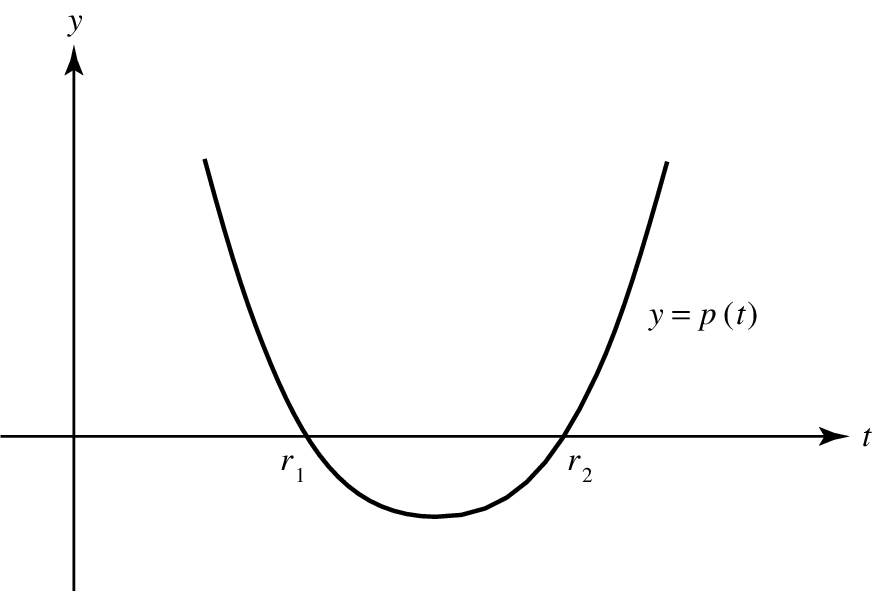
\includegraphics[width=3in,height=2in]{png/fig050101.png}
\end{center}
 \vskip6pt
 \refstepcounter{figure}
 \centerline{\bf Figure \thefigure} \label{figure:5.1.1}
 \vskip12pt


\begin{theorem} [Triangle Inequality]\label{thmtype:5.1.6}
If $\mathbf{X}$ and $\mathbf{Y}$ are in $\R^n,$ then
\begin{equation}\label{eq:5.1.6}
|\mathbf{X}+\mathbf{Y}|\le |\mathbf{X}|+|\mathbf{Y}|,
\end{equation}
with equality if and only if one of the vectors is a nonnegative
multiple of the other$.$
\end{theorem}

\proof
By definition,
\begin{equation} \label{eq:5.1.7}
\begin{array}{rcl}
|\mathbf{X}+\mathbf{Y}|^2\ar=\dst\sum^n_{i=1} (x_i+y_i)^2=\sum^n_{i=1} x^2_i+
2\sum^n_{i=1} x_iy_i+\sum^n_{i=1}y^2_i\\[4\jot]
\ar=|\mathbf{X}|^2+2(\mathbf{X}\cdot\mathbf{Y})+|\mathbf{Y}|^2\\[2\jot]
\ar\le  |\mathbf{X}|^2+2|\mathbf{X}|\,|\mathbf{Y}|+|\mathbf{Y}|^2\mbox{\quad (by
Schwarz's inequality)}\\[2\jot]
\ar=(|\mathbf{X}|+|\mathbf{Y}|)^2.
\end{array}
\end{equation}
Hence,
$$
|\mathbf{X}+\mathbf{Y}|^2\le (|\mathbf{X}|+|\mathbf{Y}|)^2.
$$
Taking square roots yields \eqref{eq:5.1.6}.


From the third line of \eqref{eq:5.1.7},
equality holds in \eqref{eq:5.1.6} if and
only  if $\mathbf{X}\cdot\mathbf{Y}=|\mathbf{X}||\mathbf{Y}|$, which is true if
and
only if one of the vectors $\mathbf{X}$ and $\mathbf{Y}$ is a nonnegative
scalar multiple of the other (Lemma~\ref{thmtype:5.1.5}).
\bbox

\begin{corollary}\label{thmtype:5.1.7}
 If $\mathbf{X},$ $\mathbf{Y},$ and
$\mathbf{Z}$ are  in $\R^n,$ then
$$
|\mathbf{X}-\mathbf{Z}|\le
|\mathbf{X}-\mathbf{Y}|+|\mathbf{Y}-\mathbf{Z}|.
$$
\end{corollary}

\proof  Write
$$
\mathbf{X}-\mathbf{Z}=(\mathbf{X}-\mathbf{Y})+(\mathbf{Y}-\mathbf{Z}),
$$
and apply Theorem~\ref{thmtype:5.1.6} with $\mathbf{X}$ and $\mathbf{Y}$
replaced by $\mathbf{X}-\mathbf{Y}$ and $\mathbf{Y}-\mathbf{Z}$.
\bbox

\begin{corollary}\label{thmtype:5.1.8}
If $\mathbf{X}$ and $\mathbf{Y}$ are
 in $\R^n,$ then
$$
|\mathbf{X}-\mathbf{Y}|\ge\left| |\mathbf{X}|-|\mathbf{Y}|\right|.
$$
\end{corollary}

\proof  Since
$$
\mathbf{X}=\mathbf{Y}+(\mathbf{X}-\mathbf{Y}),
$$
Theorem~\ref{thmtype:5.1.6} implies that
$$
|\mathbf{X}|\le |\mathbf{Y}|+|\mathbf{X}-\mathbf{Y}|,
$$
which is equivalent to
$$
|\mathbf{X}|-|\mathbf{Y}|\le |\mathbf{X}-\mathbf{Y}|.
$$
Interchanging $\mathbf{X}$ and $\mathbf{Y}$  yields
$$
|\mathbf{Y}|-|\mathbf{X}|\le |\mathbf{Y}-\mathbf{X}|.
$$
Since $|\mathbf{X}-\mathbf{Y}|=|\mathbf{Y}-\mathbf{X}|$,
the last two inequalities imply the stated conclusion.
\bbox

\begin{example}\label{example:5.1.3}\rm The {\it angle between two nonzero
vectors $\mathbf{X}=(x_1,x_2,x_3)$ and\/} $\mathbf{Y}=(y_1,y_2,y_3)$ in
$\R^3$
 is  the angle between the directed line segments
from the origin to the points $\mathbf{X}$ and $\mathbf{Y}$
(Figure~\ref{figure:5.1.2}).


\begin{center}
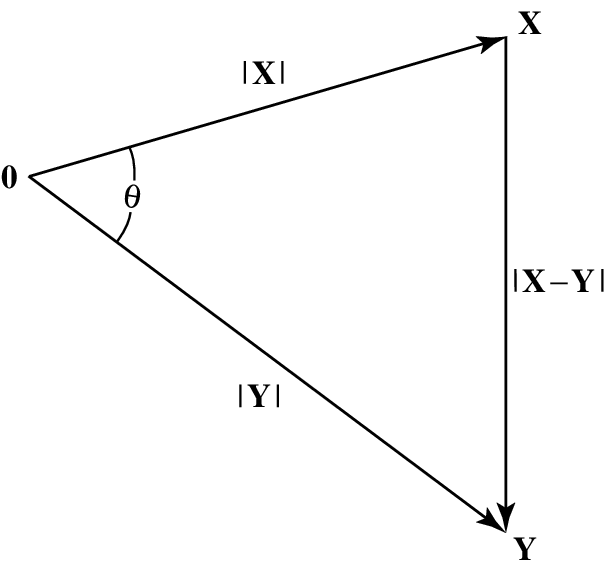
\includegraphics[width=2.1in,height=1.9in]{png/fig050102.png}
\end{center}
 \vskip6pt
 \refstepcounter{figure}
 \centerline{\bf Figure \thefigure} \label{figure:5.1.2}
 \vskip12pt

\noindent
Applying the law of cosines to the triangle
in Figure~\ref{figure:5.1.2} yields
\begin{equation}\label{eq:5.1.8}
|\mathbf{X}-\mathbf{Y}|^2=|\mathbf{X}|^2+|\mathbf{Y}|^2-2|\mathbf{X}||\mathbf{Y}|
\cos\theta.
\end{equation}
 However,
\begin{eqnarray*}
|\mathbf{X}-\mathbf{Y}|^2\ar=(x_1-y_1)^2+(x_2-y_2)^2+(x_3-y_3)^2\\[2\jot]
\ar=(x^2_1+x^2_2+x^2_3)+(y^2_1+y^2_2+y^2_3)-
2(x_1y_1+x_2y_2+x_3y_3)\\[2\jot]
\ar=|\mathbf{X}|^2+|\mathbf{Y}|^2-2\mathbf{X}\cdot\mathbf{Y}.
\end{eqnarray*}
\newpage %
\noindent
Comparing this with \eqref{eq:5.1.8} yields
$$
\mathbf{X}\cdot\mathbf{Y}=|\mathbf{X}|\,|\mathbf{Y}|\cos\theta.
$$
Since $|\cos\theta|\le1$, this verifies Schwarz's inequality in
$\R^3$.
\end{example}


\begin{example}\label{example:5.1.4}\rm Connecting the points
 $\mathbf{0}$,
$\mathbf{X}$, $\mathbf{Y}$, and $\mathbf{X}+\mathbf{Y}$ in $\R^2$ or $\R^3$
(Figure~\ref{figure:5.1.3}) produces a
parallelogram with sides of length
$|\mathbf{X}|$ and $|\mathbf{Y}|$ and a diagonal of length $|\mathbf{X}+\mathbf{Y}|$.


\vskip12pt
\begin{center}
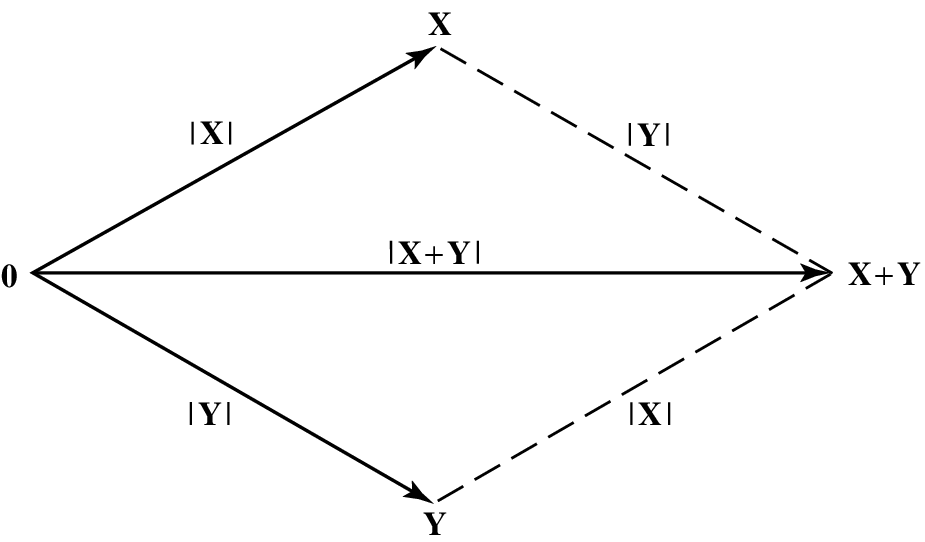
\includegraphics[width=3.1in,height=1.9in]{png/fig050103.png}
\end{center}
 \vskip6pt
 \refstepcounter{figure}
 \centerline{\bf Figure \thefigure} \label{figure:5.1.3}
 \vskip12pt

\noindent
Thus, there is a triangle with sides $|\mathbf{X}|$, $|\mathbf{Y}|$,
and
$|\mathbf{X}+\mathbf{Y}|$. From this, we see geometrically that
$$
|\mathbf{X}+\mathbf{Y}|\le |\mathbf{X}|+|\mathbf{Y}|
$$
in $\R^2$ or $\R^3$, since the length of one side of a
triangle cannot exceed the sum of the lengths of the other two. This
verifies \eqref{eq:5.1.6} for $\R^2$ and $\R^3$ and indicates
why \eqref{eq:5.1.6} is called the triangle inequality.
\bbox\end{example}





The next theorem lists properties of length, distance, and inner
product that follow directly from Definitions~\ref{thmtype:5.1.3} and
\ref{thmtype:5.1.4}. We leave the proof to you (Exercise~\ref{exer:5.1.6}).

\begin{theorem}\label{thmtype:5.1.9}
If $\mathbf{X},$ $\mathbf{Y},$ and
$\mathbf{Z}$ are members of $\R^n$ and $a$ is a scalar, then
\begin{alist}
\item % (a)
 $|a\mathbf{X}|=|a|\,|\mathbf{X}|.$
\item % (b)
 $|\mathbf{X}|\ge0,$ with equality if and only if $\mathbf{X}=
\mathbf{0}.$
\item % (c)
 $|\mathbf{X}-\mathbf{Y}|\ge0,$ with equality if and only if
$\mathbf{X}=\mathbf{Y}.$
\item % (d)
$\mathbf{X}\cdot\mathbf{Y}=\mathbf{Y}\cdot\mathbf{X}.$
\item % (e)
 $\mathbf{X}\cdot (\mathbf{Y}+\mathbf{Z})=\mathbf{X}\cdot\mathbf{Y}+
\mathbf{X}\cdot\mathbf{Z}.$
\item % (f)
 $(c\mathbf{X})\cdot\mathbf{Y}=\mathbf{X}\cdot (c\mathbf{Y})=
c(\mathbf{X}\cdot\mathbf{Y}).$
\end{alist}
\end{theorem}
         \newpage


\boxit{Line Segments in  $\pmb{\mathbb R}\mathbf{^n}$}
The equation of a line through a point $\mathbf{X}_0=(x_0,y_0,z_0)$ in
$\R^3$ can be written parametrically as
$$
x=x_0+u_1t,\quad y=y_0+u_2t,\quad z=z_0+u_3t,\quad -\infty<t<
\infty,
$$
where $u_1$, $u_2$, and $u_3$ are not all zero.  We write this in vector
form as
\begin{equation}\label{eq:5.1.9}
\mathbf{X}=\mathbf{X}_0+t\mathbf{U},\quad -\infty<t<\infty,
\end{equation}
with $\mathbf{U}=(u_1,u_2,u_3)$, and we say that the line is {\it through
$\mathbf{X}_0$ in the direction of $\mathbf{U}$\/}.

There are many ways to represent a given line parametrically. For
example,
\begin{equation}\label{eq:5.1.10}
\mathbf{X}=\mathbf{X}_0+s\mathbf{V},\quad -\infty<s<\infty,
\end{equation}
represents the same line as \eqref{eq:5.1.9}
if and only if $\mathbf{V}=a\mathbf{U}$
 for some nonzero real number $a$. Then the line is
traversed in the same direction as $s$ and $t$ vary from $-\infty$ to
$\infty$ if $a>0$, or in
 opposite directions if $a<0$.

To write the parametric equation of a line through two points
$\mathbf{X}_{0}$
 and $\mathbf{X}_1$ in $\R^3$, we take
$\mathbf{U}=\mathbf{X}_1-\mathbf{0}$
 in \eqref{eq:5.1.9}, which yields
$$
\mathbf{X}=\mathbf{X}_0+t(\mathbf{X}_1-\mathbf{X}_0)
=t\mathbf{X}_1+(1-t)\mathbf{X}_0,\quad -\infty<t<\infty.
$$
The line segment from $\mathbf{X}_0$ to $\mathbf{X}_1$ consists of those points
for which $0\le t\le1$.

\begin{example}\label{example:5.1.5}\rm   The line $L$ defined by
$$
x=-1+2t,\quad y=3-4t,\quad z=-1,\quad -\infty<t<\infty,
$$
which can be rewritten as
\begin{equation}\label{eq:5.1.11}
\mathbf{X}=(-1,3,-1)+t(2,-4,0),\quad -\infty<t<\infty,
\end{equation}
is through $\mathbf{X}_0=(-1,3,-1)$ in the direction of $\mathbf{U}=
(2,-4,0)$.  The same line can be represented by
\begin{equation}\label{eq:5.1.12}
\mathbf{X}=(-1,3,-1)+s(1,-2,0),\quad -\infty<s<\infty,
\end{equation}
or by
\begin{equation}\label{eq:5.1.13}
\mathbf{X}=(-1,3,-1)+\tau (-4,8,0),\quad -\infty<\tau<\infty.
\end{equation}
Since
$$
(1,-2,0)=\frac{1}{2}(2,-4,0),
$$
$L$ is traversed in the same direction as $t$ and $s$ vary from $-\infty$
to $\infty$ in \eqref{eq:5.1.11} and \eqref{eq:5.1.12}. However, since
$$
(-4,8,0)=-2(2,-4,0),
$$
\newpage
\noindent
$L$ is traversed in opposite directions as $t$ and $\tau$ vary from
$-\infty$ to $\infty$ in \eqref{eq:5.1.11} and~\eqref{eq:5.1.13}.


Setting $t=1$ in \eqref{eq:5.1.11}, we see that $\mathbf{X}_1=(1,-1,-1)$ is
also on $L$. The line segment from $\mathbf{X}_0$ to $\mathbf{X}_1$ consists
of all points of the form
$$
\mathbf{X}=t (1,-1,-1)+(1-t)(-1,3,-1),\quad 0\le t\le1.
$$
\end{example}

These familiar notions can be generalized to $\R^n$, as follows:

\begin{definition}\label{thmtype:5.1.10} Suppose that $\mathbf{X}_0$ and
$\mathbf{U}$ are in $\R^n$ and $\mathbf{U}\ne\mathbf{0}$. Then {\it the
line through $\mathbf{X}_0$ in the direction of\/}
$\mathbf{U}$ is the set of all points in $\R^n$ of the form
$$
\mathbf{X}=\mathbf{X}_0+t\mathbf{U},\quad -\infty<t<\infty.
$$
A set of points of the form
$$
\mathbf{X}=\mathbf{X}_0+t\mathbf{U},\quad t_1\le t\le t_2,
$$
is called a {\it line segment\/}. In particular,
the line segment from
$\mathbf{X}_0$ to $\mathbf{X}_1$ is the set of points of the form
$$
\mathbf{X}=\mathbf{X}_0+t(\mathbf{X}_1-\mathbf{X}_0)=t\mathbf{X}_1+(1-t)\mathbf{X}_0,
\quad 0\le t\le1.
$$
\end{definition}


\boxit{Neighborhoods and Open Sets in  $\pmb{\mathbb R}\mathbf{^n}$}
Having defined distance in $\R^n$, we are now able to say what we
mean by a neighborhood of a point in $\R^n$.

\begin{definition}\label{thmtype:5.1.11}
If $\epsilon>0$, the {\it $\epsilon$-neighborhood of a point\/}
$\mathbf{X}_{0}$ in
$\R^n$ is the set
$$
N_\epsilon(\mathbf{X}_0)|=\set{\mathbf{X}}{|\mathbf{X}-\mathbf{X}_0|<\epsilon}.
\eqno{\bbox}
$$
\end{definition}


An $\epsilon$-neighborhood of a point $\mathbf{X}_0$ in $\R^2$ is
the inside, but not the circumference, of the circle of radius
$\epsilon$ about $\mathbf{X}_0$. In $\R^3$ it is the
inside, but
not the surface, of the sphere of radius $\epsilon$ about $\mathbf{X}_0$.


In Section~1.3 we stated several other definitions in terms of
$\epsilon$-neighborhoods: {\it neighborhood\/}, {\it interior point\/},
{\it interior of a set\/}, {\it open set\/}, {\it closed set\/},{\it limit
point\/}, {\it boundary point\/}, {\it boundary of a set\/}, {\it closure
of a set\/}, {\it isolated point\/}, {\it exterior point\/}, and {\it
exterior of a set\/}. Since these definitions are the same for $\R^n$ as
for $\R$, we will not repeat them. We advise you to read them again in
Section~1.3, substituting $\R^n$ for $\R$ and $\mathbf{X}_{0}$ for $x_0$.


\vskip1pc
\begin{example}\label{example:5.1.6}\rm Let $S$ be the set of points in
$\R^2$ in the square bounded by the lines $x=\pm 1$, $y=\pm 1$,
except for the origin and the points on the vertical lines $x=\pm 1$
(Figure~\ref{figure:5.1.4}, page \pageref{figure:5.1.4});
thus,
$$
S=\set{(x,y)}{(x,y)\ne (0,0),\ -1<x<1,\ -1\le y\le1}.
$$
\newpage
\noindent
Every point of $S$ not on the lines $y=\pm 1$ is an
interior point, so
$$
S^0=\set{(x,y)}{(x,y)\ne (0,0),\ -1<x, y<1}.
$$
$S$ is a deleted neighborhood of $(0,0)$ and is neither open nor
closed. The closure of $S$ is
$$
\overline{S}=\set{(x,y)}{-1\le x, y\le1},
$$
and every point of $\overline S$ is a limit point of $S$. The origin
and the
perimeter of $S$ form $\partial S$, the boundary of $S$. The exterior
of $S$ consists of all points $(x,y)$ such that $|x|>1$ or $|y|>1$.
The origin is an isolated point of $S^c$.
\end{example}


\vskip12pt
\begin{center}
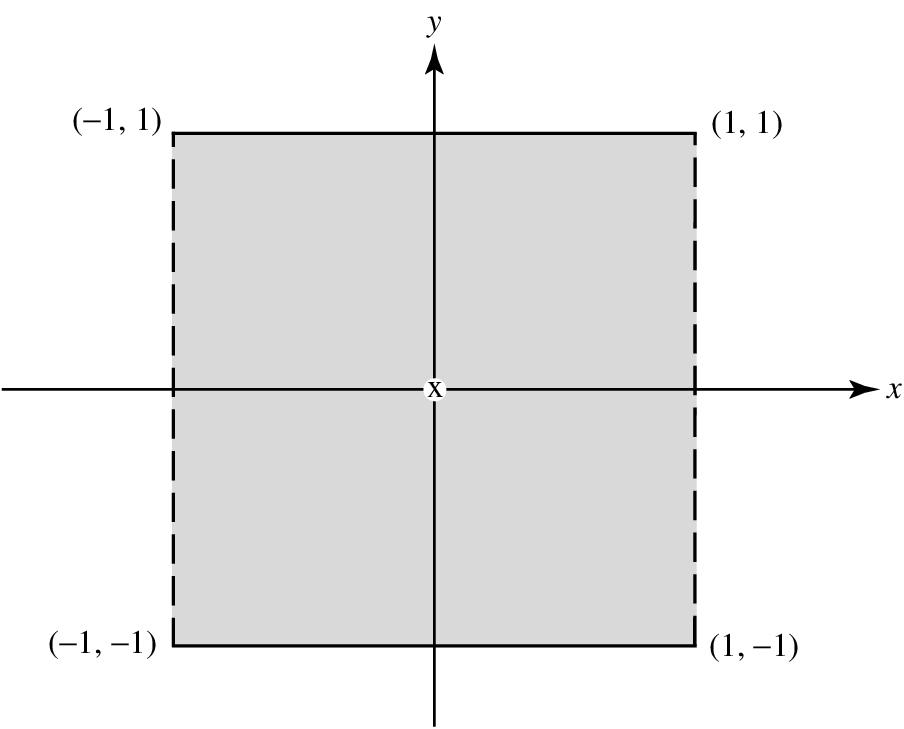
\includegraphics[width=3in,height=3.5in]{png/fig050104.png}
\end{center}
 \vskip6pt
 \refstepcounter{figure}
 \centerline{\bf Figure \thefigure} \label{figure:5.1.4}
 \vskip12pt

\begin{example}\label{example:5.1.7}\rm If $\mathbf{X}_0$ is a point in
$\R^n$
 and $r$ is a positive number, the {\it open $n$-ball of radius
$r$ about $\mathbf{X}_0$\/} is the set
$B_r(\mathbf{X}_0)=\set{\mathbf{X}}{|\mathbf{X}-\mathbf{X}_0|<r}$.
(Thus, $\epsilon$-neighborhoods are open $n$-balls.)
 If $\mathbf{X}_1$ is in $S_r(\mathbf{X}_0)$ and
$$
|\mathbf{X}-\mathbf{X}_1|<\epsilon=r-|\mathbf{X}-\mathbf{X}_0|,
$$
then $\mathbf{X}$ is in $S_r(\mathbf{X}_0)$. (The situation is depicted in
Figure~\ref{figure:5.1.5} for $n=2$.)



 Thus, $S_r(\mathbf{X}_0)$ contains an
$\epsilon$-neighborhood of each of its points, and is therefore open.
We leave it to you (Exercise~\ref{exer:5.1.13}) to show that the
closure of $B_r(\mathbf{X}_0)$ is the {\it closed\/} $n$-ball of radius
$r$ about $\mathbf{X}_0$, defined by
\newpage
$$
\overline{S}_r(\mathbf{X}_0)=\set{\mathbf{X}}{|\mathbf{X}-\mathbf{X}_0|\le
r}.
$$
\end{example}

\begin{center}
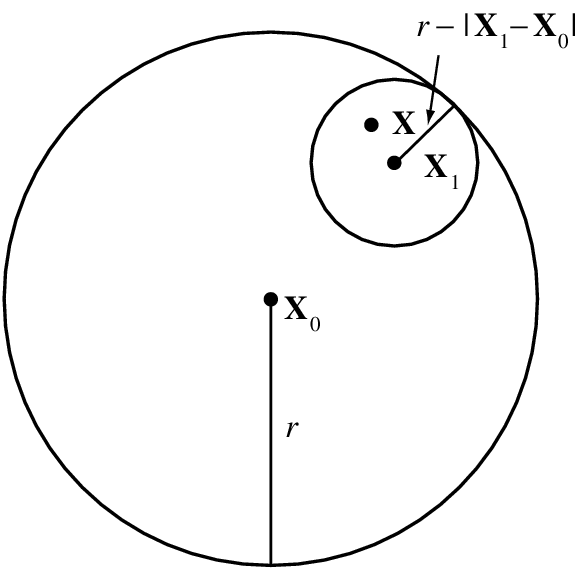
\includegraphics[width=2.05in,height=1.9in]{png/fig050105.png}
\end{center}
 \vskip6pt
 \refstepcounter{figure}
 \centerline{\bf Figure \thefigure} \label{figure:5.1.5}
 \vskip12pt


Open and closed $n$-balls are generalizations to $\R^n$ of
open and closed intervals.

The following lemma will be useful later in this section, when we consider
connected sets.


\begin{lemma}\label{thmtype:5.1.12}
If $\mathbf{X}_1$ and $\mathbf{X}_2$ are in $S_r(\mathbf{X}_0)$ for some $r>0$,
then so is every point on
the line segment from $\mathbf{X}_1$ to $\mathbf{X}_2.$
\end{lemma}

\proof
The line segment is given by
$$
\mathbf{X}=t\mathbf{X}_2+(1-t)\mathbf{X}_1,\quad 0<t<1.
$$
Suppose that $r>0$. If
$$
|\mathbf{X}_1-\mathbf{X}_0|<r,\quad |\mathbf{X}_2-\mathbf{X}_0|<r,
$$
and $0<t<1$, then
\begin{eqnarray*}
|\mathbf{X}-\mathbf{X}_0|\ar=|t\mathbf{X}_2+(1-t)\mathbf{X}_1-t\mathbf{X}_0-(1-t)\mathbf{X}_0|\\
\ar=|t(\mathbf{X}_2-\mathbf{X}_0)+(1-t)\mathbf{X}_1-\mathbf{X}_0)|\\
\ar\le  t|\mathbf{X}_2-\mathbf{X}_0|+(1-t)|\mathbf{X}_1-\mathbf{X}_0|\\
\ar< tr+(1-t)r=r.
\end{eqnarray*}
\vskip-2em\bbox\vskip2em

The proofs in Section~1.3 of
Theorem~\ref{thmtype:1.3.3} (the union of open sets is open, the
intersection of closed sets is closed) and
Theorem~\ref{thmtype:1.3.5} and its
Corollary~\ref{thmtype:1.3.6} (a set is closed if and only if it
contains all its limit points) are also valid in $\R^n$.
You
should reread them now.
\newpage
\noindent
 The Heine--Borel theorem
(Theorem~\ref{thmtype:1.3.7})
also holds in $\R^n$,
 but the proof in Section~1.3 is valid only for $n=1$. To
prove the Heine--Borel theorem for general $n$, we need some
preliminary
definitions and results that are of interest in their own right.



\begin{definition}\label{thmtype:5.1.13}
A sequence of points $\{\mathbf{X}_r\}$ in $\R^n$
{\it converges to the limit\/} $\overline{\mathbf{X}}$ if
$$
\lim_{r\to\infty} |\mathbf{X}_r-\overline{\mathbf{X}}|=0.
$$
In this case we write
$$
\lim_{r\to\infty}\mathbf{X}_r=\overline{\mathbf{X}}.
\eqno{\bbox}
$$
\end{definition}



The next two theorems follow from this, the definition of
distance in $\R^n$, and what we already know about convergence
in $\R$. We leave the proofs to you
(Exercises~\ref{exer:5.1.16} and \ref{exer:5.1.17}).

\begin{theorem}\label{thmtype:5.1.14}
Let
$$
\overline{\mathbf{X}}=(\overline{x}_1,\overline{x}_2,
\dots,\overline{x}_n)
\mbox{\quad and\quad}\mathbf{X}_r=(x_{1r}, x_{2r}, \dots, x_{nr}),\quad
r\ge1.
$$
Then $\lim_{r\to\infty}\mathbf{X}_r=\overline{\mathbf{X}}$ if and only if
$$
\lim_{r\to\infty}x_{ir}=\overline{x}_i,\quad 1\le i\le n;
$$
that is$,$ a sequence $\{\mathbf{X}_r\}$ of points in $\R^n$
converges
to a limit $\overline{\mathbf{X}}$ if and only if the sequences of
components of $\{\mathbf{X}_r\}$ converge to the respective
components of
$\overline{\mathbf{X}}.$
\end{theorem}




\begin{theorem} [Cauchy's Convergence Criterion]\label{thmtype:5.1.15}
A sequence $\{\mathbf{X}_r\}$  in $\R^n$ converges if and
only if for each $\epsilon>0$ there is an integer $K$ such that
$$
|\mathbf{X}_r-\mathbf{X}_s|<\epsilon\mbox{\quad if\quad} r,s\ge K.
$$
\end{theorem}




The next definition generalizes the definition of the diameter of a
circle or sphere.

\begin{definition}\label{thmtype:5.1.16}
If $S$ is  a nonempty subset of $\R^n$, then
$$
d(S)=\sup\set{|\mathbf{X}-\mathbf{Y}|}{\mathbf{X},\mathbf{Y}\in S}
$$
is the {\it diameter\/} of $S$.
If $d(S)<\infty,$ $S$ is  {\it bounded\/}$;$ if
$d(S)=\infty$, $S$ is {\it unbounded\/}.
\end{definition}



\begin{theorem} [Principle of Nested Sets]\label{thmtype:5.1.17}
If $S_1,$ $S_2,$ \dots\ are closed nonempty subsets of $\R^n$
such that
\begin{equation}\label{eq:5.1.14}
S_1\supset S_2\supset\cdots\supset S_r\supset\cdots
\end{equation}
and
\begin{equation}\label{eq:5.1.15}
\lim_{r\to\infty} d(S_r)=0,
\end{equation}
then the intersection
$$
I=\bigcap^\infty_{r=1}S_r
$$
contains exactly one point$.$
\end{theorem}

\newpage

\proof
Let
$\{\mathbf{X}_r\}$ be a sequence such that $\mathbf{X}_r\in S_r\ (r\ge1)$.
Because of
\eqref{eq:5.1.14}, $\mathbf{X}_r\in S_k$ if $r\ge k$, so
$$
|\mathbf{X}_r-\mathbf{X}_s|<d(S_k)\mbox{\quad if\quad} r, s\ge k.
$$
From \eqref{eq:5.1.15} and Theorem~\ref{thmtype:5.1.15},
$\mathbf{X}_{r}$
converges to a limit $\overline{\mathbf{X}}$. Since $\overline{\mathbf{X}}$ is
a limit point of every $S_k$ and every $S_k$ is closed,
$\overline{\mathbf{X}}$
is in every $S_k$ (Corollary~\ref{thmtype:1.3.6}).
Therefore, $\overline{\mathbf{X}}\in I$, so $I\ne
\emptyset$. Moreover, $\overline{\mathbf{X}}$ is the only point in $I$,
since if $\mathbf{Y}\in I$, then
$$
|\overline{\mathbf{X}}-\mathbf{Y}|\le d(S_k),\quad k\ge1,
$$
and \eqref{eq:5.1.15} implies that $\mathbf{Y}=\overline{\mathbf{X}}$.
\bbox


We can now prove the Heine--Borel theorem for $\R^n$. This
theorem
concerns {\it compact\/} sets. As in $\R$, a compact set in
$\R^n$ is a  closed and bounded set.

Recall that
a collection  ${\mathcal H}$  of open sets is an open covering of a set
$S$ if
$$
S\subset\cup\set{H}{ H\in {\mathcal H}}.
$$


\begin{theorem} [Heine--Borel Theorem]\label{thmtype:5.1.18}
If ${\mathcal H}$ is an open covering of a compact subset $S,$
 then $S$ can be covered
by finitely many sets from ${\mathcal H}.$
\end{theorem}

\proof
The proof is by contradiction. We first consider the case where
$n=2$, so that you can  visualize  the method. Suppose that
there is a covering
${\mathcal H}$ for $S$ from which it is impossible to select a finite
subcovering. Since $S$ is bounded, $S$ is contained in a closed square
$$
T=\{(x,y)|a_1\le x\le a_1+L, a_2\le x\le a_2+L\}
$$
with sides of length $L$ (Figure~\ref{figure:5.1.6}).

 \vspace*{12pt}
\begin{center}
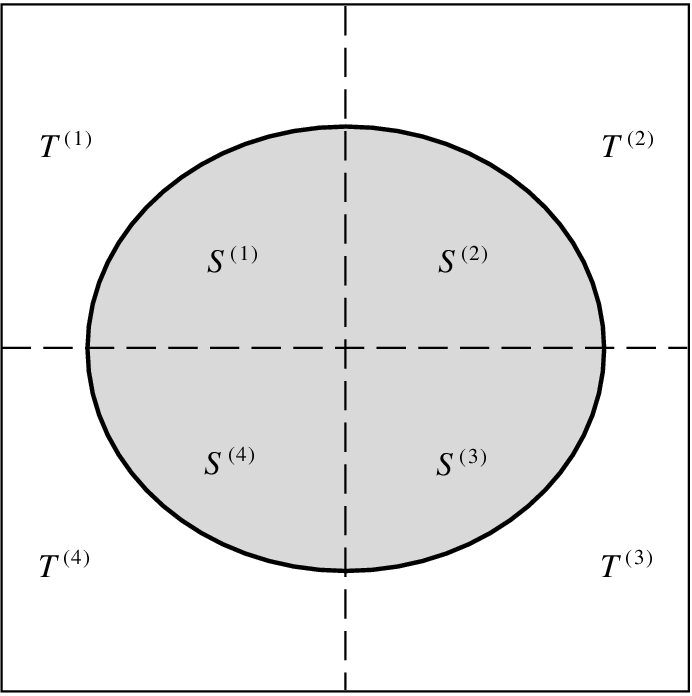
\includegraphics[width=2.3in,height=2.3in]{png/fig050106.png}
\end{center}
 \vskip6pt
 \refstepcounter{figure}
 \centerline{\bf Figure \thefigure} \label{figure:5.1.6}
 \vskip12pt

Bisecting the sides
of $T$ as shown by the dashed lines in Figure~\ref{figure:5.1.6} leads to
four closed squares, $T^{(1)}, T^{(2)}$, $T^{(3)}$, and $T^{(4)}$,
with sides of length $L/2$. Let
$$
S^{(i)}=S\cap T^{(i)},\quad 1\le i\le4.
$$
Each $S^{(i)}$, being the intersection of closed sets, is closed, and
$$
S=\bigcup^4_{i=1} S^{(i)}.
$$
Moreover, ${\mathcal H}$ covers each $S^{(i)}$, but at least one $S^{(i)}$
cannot be covered by any finite subcollection of ${\mathcal H}$, since if all
the $S^{(i)}$ could be, then so could $S$. Let $S_1$ be a set with
this property, chosen from $S^{(1)}$, $S^{(2)}$, $S^{(3)}$, and
$S^{(4)}$. We are now back to the situation we started from: a
compact set $S_1$ covered by ${\mathcal H}$, but not by any finite
subcollection of ${\mathcal H}$. However, $S_1$ is contained in
a square
$T_1$ with sides of length $L/2$ instead of $L$. Bisecting the sides
of $T_1$ and repeating the argument, we obtain a subset $S_2$ of $S_1$
that has the same properties as $S$, except that it is contained in a
square with sides of length $L/4$. Continuing in this way produces a
sequence of nonempty closed sets $S_0\,(=S)$, $S_1$, $S_2$, \dots,
such
that $S_k\supset S_{k+1}$ and $d(S_k)\le L/2^{k-1/2}\,(k\ge0)$.
From Theorem~\ref{thmtype:5.1.17}, there is a point $\overline{\mathbf{X}}$ in
$\bigcap^\infty_{k=1}S_k$. Since $\overline{\mathbf{X}}\in S$, there is an
open set $H$ in ${\mathcal H}$ that contains $\overline{\mathbf{X}}$, and
this $H$ must also contain some $\epsilon$-neighborhood of
$\overline{\mathbf{X}}$. Since every $\mathbf{X}$ in $S_k$ satisfies
the inequality
$$
|\mathbf{X}-\overline{\mathbf{X}}|\le2^{-k+1/2}L,
$$
it follows that $S_k\subset H$ for $k$ sufficiently large. This
contradicts our assumption on ${\mathcal H}$, which led us to believe that
no $S_k$ could be covered by a finite number of sets from ${\mathcal H}$.
Consequently, this assumption must be false: ${\mathcal H}$ must have a
finite subcollection that covers $S$. This completes the proof for $n=2$.


The idea of the proof is the same for $n>2$. The counterpart of the
square $T$ is the {\it hypercube\/} with sides of
length
$L$:
$$
T=\set{(x_1,x_2, \dots,x_n)}{ a_i\le x_i\le a_i+L, i=1,2, \dots, n}.
$$
Halving the intervals of variation of the $n$ coordinates
$x_1$, $x_2$, \dots, $x_n$ divides $T$ into $2^n$ closed hypercubes
with sides of length $L/2$:
$$
T^{(i)}=\set{(x_1,x_2, \dots,x_n)}{b_i\le x_i\le b_i+L/2,
1\le i\le n},
$$
where $b_i=a_i$ or $b_i=a_i+L/2$. If no finite subcollection of ${\mathcal
H}$ covers $S$, then at least one of these smaller hypercubes must
contain a subset of $S$ that is not covered by any finite subcollection
of $S$. Now the proof proceeds as for $n=2$.
\bbox

The Bolzano--Weierstrass theorem
is valid in $\R^n$; its proof is the
same as in $\R$.

\boxit{Connected Sets and Regions}
Although it is legitimate to consider functions defined on arbitrary
domains, we \pagebreak restricted our study of functions of one
variable mainly
to functions defined on intervals. There are good reasons for this. If
we wish to raise questions of continuity and differentiability at
every point of the domain $D$ of a function $f$, then every point of
$D$ must be a limit point of $D^0$. Intervals have this property.
Moreover, the definition of $\int_a^b f(x)\,dx$ is obviously
applicable only if $f$ is defined on $[a,b]$.

It is not productive
to consider questions of continuity and
differentiability of functions defined on the union of disjoint
intervals,  since many important results
simply do not hold for such domains. For example, the intermediate
 value theorem (Theorem~\ref{thmtype:2.2.10}; see also
Exercise~\ref{exer:2.2.25}) says that if $f$ is
continuous on an
interval $I$ and $f(x_1)<\mu<f(x_2)$ for some $x_1$ and $x_2$ in $I$,
then $f(\overline{x})=\mu$ for some $\overline{x}$ in $I$.
Theorem~\ref{thmtype:2.3.12} says that $f$ is constant on an
interval $I$ if $f'\equiv0$ on $I$. Neither of these results holds if
$I$ is the union of disjoint intervals rather than a single interval;
thus, if $f$ is defined on $I=(0,1)\cup (2,3)$ by
$$
f(x)=\left\{\casespace\begin{array}{ll} 1,&0<x<1,\\
0,&2<x<3,\end{array}\right.
$$
then $f$ is continuous on $I$, but does not assume any value between
$0$ and $1$, and $f'\equiv0$ on $I$, but $f$ is not constant.

It is not difficult to see why these results fail to hold for this
function: the domain of $f$ consists of two disconnected pieces. It
would be
more sensible to regard $f$ as two entirely different functions, one
defined on $(0,1)$ and the other on $(2,3)$. The two results mentioned
are valid for each of these functions.

As we will see when we study functions defined on subsets of
$\R^n$,
 considerations like those just cited as making it natural to
consider functions defined on intervals in $\R$ lead us to
single out a preferred class of subsets as domains of functions of $n$
variables. These subsets are called {\it regions\/}. To
define this term, we first need the following definition.


\begin{definition}\label{thmtype:5.1.19}
A subset $S$ of $\R^n$ is
 {\it connected\/} if it is impossible to represent
$S$ as the union of two
disjoint nonempty sets such that neither contains a limit point of the
other; that is, if $S$ cannot be expressed as $S=A\cup B$, where
\begin{equation}\label{eq:5.1.16}
A\ne\emptyset,\quad B\ne\emptyset,\quad\overline{A}\cap B=
\emptyset,\mbox{\quad and\quad} A\cap\overline{B}=\emptyset.
\end{equation}
If $S$ can be expressed in this way, then $S$ is
{\it disconnected\/}.
\end{definition}

\begin{example}\label{example:5.1.8}\rm The empty set and singleton sets
are connected, because they cannot be represented as the union of two
disjoint nonempty sets.
\end{example}

\begin{example}\label{example:5.1.9}\rm The space $\R^n$ is
connected, because if $\R^n=A\cup B$ with $\overline{A}\cap
B=\emptyset$ and $A\cap\overline{B}=\emptyset$, then
$\overline{A}\subset A$ and $\overline{B}\subset B$; that is, $A$ and
$B$ are both closed and therefore are both open. Since the only
nonempty subset
of $\R^n$ that is both open and closed is $\R^n$ itself
(Exercise~\ref{exer:5.1.21}), one of $A$ and $B$ is $\R^n$ and
the other is empty.
\end{example}

\topfig{-3}
\begin{center}
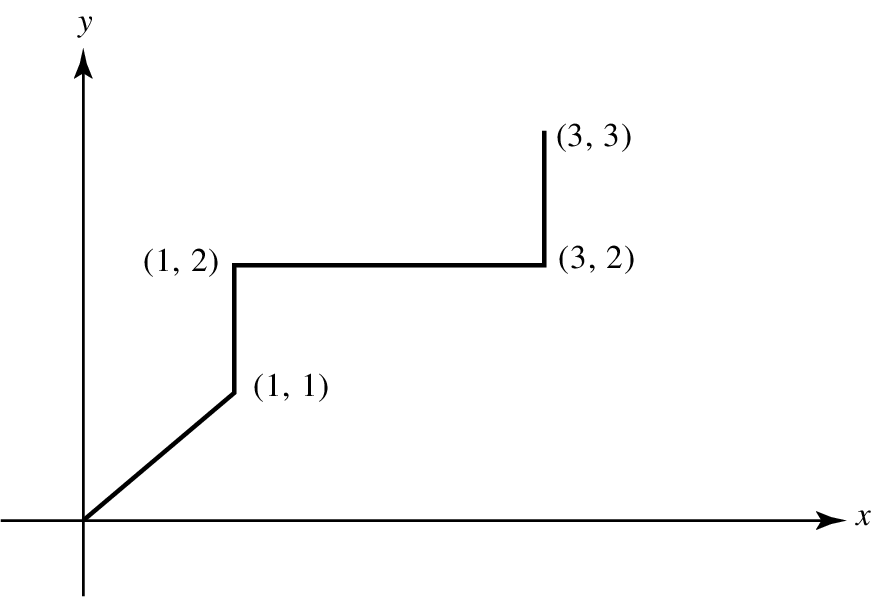
\includegraphics[width=3in,height=2.1in]{png/fig050107.png}
\end{center}
 \vskip6pt
 \refstepcounter{figure}
 \centerline{\bf Figure \thefigure} \label{figure:5.1.7}
 \vskip12pt

If $\mathbf{X}_1,\mathbf{X}_2, \dots,\mathbf{X}_k$ are points in $\R^n$ and
$L_i$ is the line segment from $\mathbf{X}_i$ to $\mathbf{X}_{i+1}$,
$1\le i\le k-1$, we say that $L_1$, $L_2$, \dots, $L_{k-1}$ form a
{\it polygonal path\/}
 from $\mathbf{X}_1$ to $\mathbf{X}_k$, and that $\mathbf{X}_{1}$
 and
$\mathbf{X}_k$ are {\it connected\/} by the polygonal path. For example,
Figure~\ref{figure:5.1.7} shows a polygonal
path in
$\R^2$ connecting $(0,0)$ to $(3,3)$. A set $S$ is {\it polygonally
connected\/} if
every pair of points in $S$ can be connected by a polygonal path lying
entirely in $S$.



\begin{theorem}\label{thmtype:5.1.20}
 An open set $S$ in $\R^n$ is
connected if and only if it is polygonally connected$.$
\end{theorem}

\proof
For sufficiency, we will show that if $S$ is disconnected, then
$S$ is not poly\-gonally connected. Let $S=A\cup B$, where $A$ and $B$
satisfy \eqref{eq:5.1.16}. Suppose that $\mathbf{X}_1\in A$ and $\mathbf{X}_2\in
B$, and assume that there is a polygonal path in $S$ connecting
$\mathbf{X}_{1}$ to $\mathbf{X}_2$. Then some line segment $L$ in this
path must
contain a point $\mathbf{Y}_1$ in $A$ and a point $\mathbf{Y}_2$ in $B$. The
line segment
$$
\mathbf{X}=t\mathbf{Y}_2+(1-t)\mathbf{Y}_1,\quad 0\le t\le1,
$$
is part of $L$ and therefore in $S$.  Now define
$$
\rho=\sup\set{\tau}{ tY_2+(1-t)\mathbf{Y}_1\in A,\ 0\le t\le
\tau\le1},
$$
and let
$$
\mathbf{X}_\rho=\rho\mathbf{Y}_2+(1-\rho)\mathbf{Y}_1.
$$
Then $\mathbf{X}_\rho\in\overline{A}\cap\overline{B}$. However, since
$\mathbf{X}_\rho\in A\cup B $ and $\overline{A}\cap
B=A\cap\overline{B}=\emptyset$, this is impossible. Therefore,
the assumption that there is a polygonal path in $S$
from $\mathbf{X}_1$ to $\mathbf{X}_2$ must be false.


For necessity, suppose that $S$ is a connected open set and $\mathbf{X}_0\in
S$. Let $A$ be the set consisting of $\mathbf{X}_0$ and the points in $S$
can be connected to $\mathbf{X}_0$ by polygonal paths in $S$. Let $B$ be
set of points in $S$ that cannot be connected to $\mathbf{X}_0$
by polygonal paths.
 If $\mathbf{Y}_0\in S$, then $S$ contains an
$\epsilon$-neighborhood $N_\epsilon (\mathbf{Y}_0)$ of $\mathbf{Y}_0$,
since $S$ is open. Any point $\mathbf{Y}_1$ in $N_\epsilon
(\mathbf{Y}_{0}$
 can be connected to $\mathbf{Y}_0$ by the line segment
$$
\mathbf{X}=t\mathbf{Y}_1+(1-t)\mathbf{Y}_0,\quad 0\le t\le1,
$$
which lies in $N_\epsilon(\mathbf{Y}_0)$ (Lemma~\ref{thmtype:5.1.12}) and
therefore in
$S$. This implies that $\mathbf{Y}_0$ can be connected to $\mathbf{X}_0$ by a
polygonal path in $S$ if and only if every member of  $N_\epsilon
(\mathbf{Y}_{0})$
 can also. Thus, $N_\epsilon(\mathbf{Y}_0)\subset A$ if $\mathbf{Y}_0\in
A$, and $N_\epsilon (\mathbf{Y}_0)\in B$ if $\mathbf{Y}_0\in B$. Therefore,
$A$ and $B$ are open. Since $A\cap B =\emptyset$, this implies that
$A\cap\overline{B}=\overline{A}\cap B=\emptyset$
(Exercise~\ref{exer:5.1.14}). Since $A$ is nonempty $(\mathbf{X}_0\in A)$,
it
now follows that $B=\emptyset$, since if $B\ne\emptyset$, $S$ would be
disconnected (Definition~\ref{thmtype:5.1.19}). Therefore, $A=S$, which
completes the proof of necessity.
\bbox

We did not use the assumption that $S$ is
open
in the proof of sufficiency.
In fact, we actually proved that any polygonally connected
set, open or not, is connected. The converse is false. A set (not
open) may be connected but not polygonally connected
(Exercise~\ref{exer:5.1.29}).

Our study of functions on $\R^n$ will deal mostly with functions
whose domains are regions, defined next.


\begin{definition}\label{thmtype:5.1.21}
A {\it region\/} $S$ in $\R^n$ is the union of an open connected
set
with some, all, or none of its boundary; thus, $S^0$ is connected, and
every point of $S$ is a limit point of $S^0$.
\end{definition}



\begin{example}\label{example:5.1.10}\rm Intervals are the only
regions in $\R$ (Exercise~\ref{exer:5.1.31}). The $n$-ball
$B_r(\mathbf{X}_0)$ (Example~\ref{example:5.1.7}) is a region in $\R^n$,
as is its closure $\overline{S}_r(\mathbf{X}_0)$. The set
$$
S=\set{(x,y)}{x^2+y^2\le1\mbox{\quad or\quad} x^2+y^2\ge4}
$$
(Figure~\ref{figure:5.1.8}\part{a}, page~\pageref{figure:5.1.8}) is not a
region in
$\R^2$, since it
is not connected. The set $S_1$ obtained by adding the line segment
$$
L_1\colon\quad\mathbf{X}=t(0,2)+(1-t)(0,1),\quad 0<t<1,
$$
to $S$ (Figure~\ref{figure:5.1.8}\part{b}) is connected but is not a
region, since points on the line segment are not limit points of
$S^0_1$. The set $S_2$ obtained by adding to $S_1$ the points
in the first quadrant bounded
by the circles $x^2+y^2=1$ and $x^2+y^2=4$ and the line segments $L_1$
and
$$
L_2\colon\quad X=t(2,0)+(1-t)(1,0),\quad 0<t<1
$$
(Figure~\ref{figure:5.1.8}\part{c}), is a region.
\end{example}

\vspace*{-12pt}
\boxit{More about Sequences in $\pmb{\mathbb R}\mathbf{^n}$}
From Definition~\ref{thmtype:5.1.13}, a sequence $\{\mathbf{X}_r\}$ of points
in
$\R^n$ converges to a limit $\overline{\mathbf{X}}$ if and only if
for every $\epsilon>0$ there is an integer $K$ such that
$$
|\mathbf{X}_r-\overline{\mathbf{X}}|<\epsilon\mbox{\quad if\quad} r\ge K.
$$
\newpage
\noindent
The $\R^n$ definitions of divergence, boundedness, subsequence,
and sums, differences, and constant multiples of sequences are
analogous to those given in Sections 4.1 and 4.2 for the case where
$n=1$. Since $\R^n$ is not ordered for $n>1$, monotonicity,
limits inferior and superior of sequences in $\R^n$, and
divergence to $\pm\infty$ are  undefined for $n>1$. Products
and quotients of members of $\R^n$ are also undefined if $n>1$.

\vskip24pt
\begin{center}
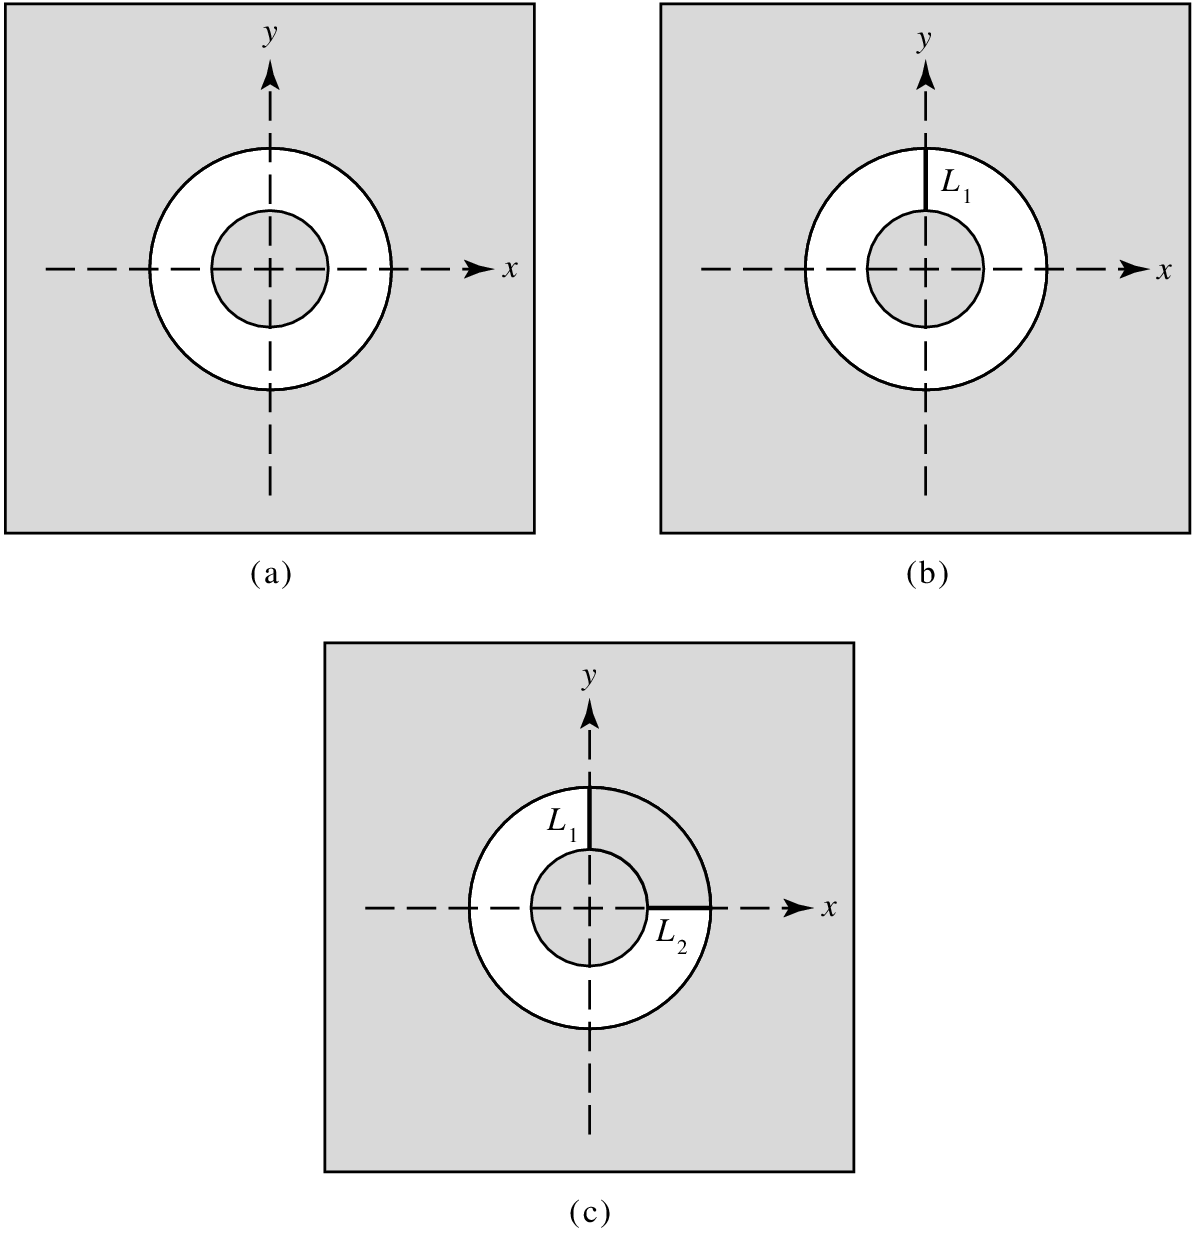
\includegraphics[width=3.95in,height=4.2in]{png/fig050108.png}
\end{center}
 \vskip6pt
 \refstepcounter{figure}
 \vskip12pt
 \centerline{\bf Figure \thefigure} \label{figure:5.1.8}
 \vskip12pt

Several theorems from Sections~4.1 and 4.2 remain valid
for sequences in $\R^n$, with proofs unchanged, provided that
``$|\quad
|$" is interpreted as distance in $\R^n$. (A trivial change is
required: the subscript $n$, used in Sections~4.1 and 4.2
to identify the terms of the sequence, must be replaced,
since $n$ here stands for the dimension of the space.) These
include Theorems~\ref{thmtype:4.1.2} (uniqueness of the limit),
\ref{thmtype:4.1.4} (boundedness of a convergent sequence),
parts of \ref{thmtype:4.1.8} (concerning limits of sums,
differences, and constant multiples of convergent sequences), and
 \ref{thmtype:4.2.2} (every subsequence of a
convergent sequence converges to the limit of the sequence).

\newpage
\exercises

\noindent{\it
With $\R$ replaced by $\R^n$, the following exercises from
Section~$1.3$ are also suitable for this section:
 $\ref{exer:1.3.7}$-$\ref{exer:1.3.10},$
$\ref{exer:1.3.12}$-$\ref{exer:1.3.15},$
$\ref{exer:1.3.19},$
$\ref{exer:1.3.20}$ $($except \part{e}$),$ and
$\ref{exer:1.3.21}.$}

\begin{exerciselist}


\item\label{exer:5.1.1} Find $a\mathbf{X}+b\mathbf{Y}$.
\begin{alist}
\item % (a)
 $\mathbf{X}=(1,2,-3,1)$,\quad $\mathbf{Y}=(0,-1,2,0)$, $a=3$, $b=6$
\item % (b)
 $\mathbf{X}=(1,-1,2)$,\quad $\mathbf{Y}=(0,-1,3)$, $a=-1$, $b=2$
\item % (c)
 $\mathbf{X}=(\frac{1}{2},\frac{3}{2},\frac{1}{4},\frac{1}{6})$,\quad
$\mathbf{Y}=(-\frac{1}{2},1,5,\frac{1}{3})$, $a=\frac{1}{2}$,
$b=\frac{1}{6}$
\end{alist}


\item\label{exer:5.1.2} Prove Theorem~\ref{thmtype:5.1.2}.

\item\label{exer:5.1.3} Find $|\mathbf{X}|$.

\begin{tabular}[t]{@{}p{168pt}@{}p{168pt}}
 \part{a} $(1,2,-3,1)$&\part{b}
$\left(\frac{1}{2},\frac{1}{3},\frac{1}{
4},\frac{1}{6}\right)$\\
 \part{c} $(1,2,-1,3,4)$&\part{d} $(0,1,0,-1,0,-1)$\\
\end{tabular}

\item\label{exer:5.1.4} Find $|\mathbf{X}-\mathbf{Y}|$.
\begin{alist}
\item % (a)
 $\mathbf{X}=(3,4,5,-4)$,\quad $\mathbf{Y}=(2,0,-1,2)$
\item % (b)
 $\mathbf{X}=(-\frac{1}{2},\frac{1}{2},\frac{1}{4},-\frac{1}{4})$,\quad
$\mathbf{Y}=(\frac{1}{3},-\frac{1}{6},\frac{1}{6},-\frac{1}{3})$
\item % (c)
 $\mathbf{X}=(0,0,0)$,\quad $\mathbf{Y}=(2,-1,2)$
\item % (d)
 $\mathbf{X}=(3,-1,4,0,-1)$,\quad $\mathbf{Y}=(2,0,1,-4,1)$
\end{alist}

\item\label{exer:5.1.5} Find $\mathbf{X}\cdot\mathbf{Y}$.
\begin{alist}
\item % (a)
 $\mathbf{X}=(3,4,5,-4)$,\quad $\mathbf{Y}=(3,0,3,3)$
\item % (b)
 $\mathbf{X}=(\frac{1}{6},\frac{11}{12},\frac{9}{8},\frac{5}{2})$,\quad
$\mathbf{Y}=(-\frac{1}{2}, \frac{1}{2},\frac{1}{4},-\frac{1}{4})$
\item % (c)
 $\mathbf{X}=(1,2,-3,1,4)$,\quad $\mathbf{Y}=(1,2,-1,3,4)$
\end{alist}



\item\label{exer:5.1.6} Prove Theorem~\ref{thmtype:5.1.9}.

\item\label{exer:5.1.7} Find a parametric equation of the line through
$\mathbf{X}_0$ in the direction of $\mathbf{U}$.
\begin{alist}
\item % (a)
 $\mathbf{X}_0=(1,2,-3,1)$,\quad $\mathbf{U}=(3,4,5,-4)$
\item % (b)
 $\mathbf{X}_0=(2,0,-1,2,4)$,\quad $\mathbf{U}=(-1,0,1,3,2)$
\item % (c)
 $\mathbf{X}_0=(-\frac{1}{2},\frac{1}{2},\frac{1}{4},-\frac{1}{
4})$,\quad
$\mathbf{U}=(\frac{1}{3},-\frac{1}{6},\frac{1}{6},-\frac{1}{3})$
\end{alist}

\item\label{exer:5.1.8}
Suppose that $\mathbf{U}\ne\mathbf{0}$ and $\mathbf{V}\ne\mathbf{0}$.
 Complete the sentence:  The equations
$$
\mathbf{X}=\mathbf{X}_0+t\mathbf{U},\quad -\infty<t<\infty,
$$
and
$$
\mathbf{X}=\mathbf{X}_1+s\mathbf{V},\quad -\infty<s<\infty,
$$
represent the same line in
$\R^n$ if and only if ...

\item\label{exer:5.1.9} Find the equation of the line segment from
$\mathbf{X}_{0}$ to $\mathbf{X}_1$.
\begin{alist}
\item % (a)
 $\mathbf{X}_0=(1,-3,4,2)$,\quad $\mathbf{X}_1=(2,0,-1,5)$
\item % (b)
$\mathbf{X}_0=(3,1-2,1,4)$,\quad $\mathbf{X}_1=(2,0,-1,4,-3)$
\nopagebreak
\item % (c)
 $\mathbf{X}_0=(1,2,-1)$,\quad $\mathbf{X}_1=(0,-1,-1)$
\end{alist}
\newpage

\item\label{exer:5.1.10} Find $\sup\set{\epsilon}{ N_\epsilon(\mathbf{X}_0)
\subset S}$.
\begin{alist}
\item % (a)
 $\mathbf{X}_0=(1,2,-1,3)$; $S=\mbox{the open 4-ball of
radius 7 about $(0,3,-2,2)$}$
\item % (b)
 $\mathbf{X}_0=(1,2,-1,3)$; $S=\set{(x_1,x_2,x_3,x_4)}
{|x_i|\le5, 1\le i\le4}$
\item % (c)
 $\mathbf{X}_0=(3,\frac{5}{2})$; $S=\mbox{the closed triangle
with vertices $(2,0)$, $(2,2)$, and $(4,4)$}$
\end{alist}

\item\label{exer:5.1.11} Find \part{i} $\partial S$; \part{ii} $\overline{S}$;
\part{iii} $S^0$; \part{iv} exterior of $S$.
\begin{alist}
\item % (a)
 $S=\set{(x_1,x_2,x_3,x_4)}{|x_i|<3, i=1,2,3}$
\item % (b)
 $S=\set{(x,y,1)}{ x^2+y^2\le1}$
\end{alist}

\item\label{exer:5.1.12} Describe the following sets as open, closed, or neither.
\begin{alist}
\item % (a)
 $S=\set{(x_1,x_2,x_3,x_4)}{|x_1|>0, x_2<1, x_3\ne-2}$
\item % (b)
 $S=\set{(x_1,x_2,x_3,x_4)}{ x_1=1, x_3\ne-4}$
\item % (c)
 $S=\set{(x_1,x_2,x_3,x_4)}{ x_1=1,-3\le x_2\le1, x_4=-5}$
\end{alist}

\item\label{exer:5.1.13} Show that the closure of the open $n$-ball
$$
B_r(\mathbf{X}_0)=\set{\mathbf{X}}{|\mathbf{X}-\mathbf{X}_0|<r}
$$
is the closed $n$-ball
$$
\overline{B}_r(\mathbf{X}_0)=\set{\mathbf{X}}{|\mathbf{X}-\mathbf{X}_0|\le
r}.
$$

\item\label{exer:5.1.14} Prove: If $A$ and $B$ are open and $A\cap
B=\emptyset$, then $A\cap\overline{B}=\overline{A}\cap B=\emptyset$.

\item\label{exer:5.1.15} Show that if $\lim_{r\to\infty}\mathbf{X}_r$ exists,
then it is unique.

\item\label{exer:5.1.16} Prove Theorem~\ref{thmtype:5.1.14}.

\item\label{exer:5.1.17} Prove Theorem~\ref{thmtype:5.1.15}.

\item\label{exer:5.1.18} Find $\lim_{r\to\infty}\mathbf{X}_r$.
\begin{alist}
\item % (a)
 $\mathbf{X}_r=\dst\left(r\sin\frac{\pi}{r},\cos\frac{\pi}{r},
e^{-r}\right)$
\item % (b)
$\mathbf{X}_r=\dst\left(1-\frac{1}{r^2},\log\frac{r+1}{r+2},\left(1+\frac{1}{r}\right)^r\right)$
\end{alist}

\item\label{exer:5.1.19} Find $d(S)$.
\begin{alist}
\item % (a)
 $S=\set{(x,y,x)}{|x|\le2, |y|\le1, |z-2|\le2}$
\item % (b)
 $\dst{S=\set{(x,y)}{\frac{(x-1)^2}{9}+\frac{(y-2)^2}{4}=1}}$
\item % (c)
 $S=\mbox{the triangle in $\R^2$ with vertices
$(2,0)$, $(2,2)$, and $(4,4)$}$
\item % (d)
 $S=\set{(x_1,x_2, \dots,x_n)}{|x_i|\le L,i=1,2, \dots,n}$
\item % (e)
 $S=\set{(x,y,z)}{ x\ne0, |y|\le1,z>2}$
\end{alist}

\item\label{exer:5.1.20} Prove that $d(S)=d(\overline{S})$ for any set $S$
in $\R^n$.

\item\label{exer:5.1.21} Prove: If a nonempty subset $S$ of $\R^n$
is both open and closed, then $S=\R^n$.

\newpage % 301

\item\label{exer:5.1.22}
Use the Bolzano--Weierstrass theorem to show that
if $S_1$, $S_2$, \dots, $S_m$, \dots\ is an infinite sequence of
nonempty compact
sets and $S_1\supset S_2\supset\cdots\supset S_m\supset\cdots$, then
$\bigcap^\infty_{m=1}S_m$ is nonempty. Show that the conclusion does
not follow if the sets are assumed to be closed rather than compact.

\item\label{exer:5.1.23} Suppose that a sequence $U_1$, $U_2$, \dots\ of open
sets covers a compact set $S$. Without using the Heine--Borel theorem,
show that $S\subset\bigcup^N_{m=1}U_m$ for some $N$.
\hint{Apply Exercise~$\ref{exer:5.1.22}$ to the sets
$S_n=S\cap\left(\bigcup^n_{m=1} U_m\right)^c.$}

(This is a seemingly restricted version of the Heine--Borel theorem,
valid for the case where the covering collection ${\mathcal H}$ is
denumerable. However, it can be shown that there is no loss of
generality in assuming this.)

\item\label{exer:5.1.24}
The {\it distance from a point $\mathbf{X\/}_0$ to a
nonempty set $S$\/} is
defined by
$$
\dist(\mathbf{X}_0, S)=\inf\set{|\mathbf{X}-\mathbf{X}_0|}
{\mathbf{X}\in S}.
$$
\begin{alist}
\item % (a)
Prove:  If $S$ is closed and $\mathbf{X}_0\in \R^n$,
there is a point $\overline{\mathbf{X}}$ in $S$ such that
$$
|\overline{\mathbf{X}}-\mathbf{X}_0|=\dist (\mathbf{X}_0, S).
$$
\hint{Apply  Exercise~$\ref{exer:5.1.22}$ to the sets
$$
C_m=\set{\mathbf{X}}{\mathbf{X}\in S\mbox{ and } |\mathbf{X}-\mathbf{X}_0|\le
\dist(\mathbf{X}_0,S)+1/m},\quad m\ge 1.
$$}
\item % (b)
Show that if $S$ is closed and $\mathbf{X}_0
\not\in S$, then $\dist (\mathbf{X}_0,S)>0$.
\item % (c)
 Show that the conclusions of  \part{a} and \part{b} may fail to
hold if $S$ is not closed.
\end{alist}

\item\label{exer:5.1.25}
The {\it distance between two nonempty sets $S$
and $T$\/} is defined by
$$
\dist(S,T)=\inf\set{|\mathbf{X}-\mathbf{Y}|}{\mathbf{X}\in S,
\mathbf{Y}\in T}.
$$
\begin{alist}
\item % (a)
 Prove:  If $S$ is closed and  $T$ is compact, there are points
$\overline{\mathbf{X}}$ in $S$ and $\overline{\mathbf{Y}}$ in $T$ such
that
$$
|\overline{\mathbf{X}}-\overline{\mathbf{Y}}|=\dist(S,T).
$$
\hint{Use Exercises~$\ref{exer:5.1.22}$ and $\ref{exer:5.1.24}.$}
\item % (b)
Under the assumptions of \part{a}, show that  $\dist(S,T)>0$
if $S\,\cap\, T=\emptyset$.
\item % (c)
 Show that the conclusions of  \part{a} and \part{b} may fail to
hold if $S$ or $T$ is not closed or $T$ is unbounded.
\end{alist}

\item\label{exer:5.1.26}
\begin{alist}
\item % (a)
Prove: If a compact set $S$ is contained in an open set $U$, there is
a positive number $r$ such that the set
$$
S_r=\set{\mathbf{X}}{\dist (\mathbf{X}, S)\le r}
$$
is contained in $U$.  (You will need Exercise~\ref{exer:5.1.24} here.)
\item % (b)
 Show that $S_r$ is compact.
\end{alist}

\item\label{exer:5.1.27}
 Let $D_1$ and $D_2$ be compact subsets of $\R^n$.
 Show that
$$
D=\set{(\mathbf{X},\mathbf{Y})}{\mathbf{X}\in D_1,\mathbf{Y}\in D_2}
$$
is a compact subset of $\mathbf{R}^{2n}$.

\item\label{exer:5.1.28}
 Prove: If $S$ is open and $S=A\cup B$ where
$\overline{A}\cap B=A\cap\overline{B}=\emptyset$, then $A$ and $B$ are
open.

\item\label{exer:5.1.29} Give an example of a connected set in $\R^n$
 that is not polygonally connected.

\item\label{exer:5.1.30}
Prove that a region is connected.

\item\label{exer:5.1.31} Show that the intervals are the only regions in
$\R$.

\item\label{exer:5.1.32}
 Prove: A bounded sequence in $\R^n$ has a
convergent subsequence. \hint{Use Theorems~$\ref{thmtype:5.1.14},$
$\ref{thmtype:4.2.2},$ and
$\ref{thmtype:4.2.5}\part{a}.$}

\item\label{exer:5.1.33} Define ``$\lim_{r\to\infty}\mathbf{X}_r=\infty$'' if
$\{\mathbf{X}_r\}$ is a sequence in $\R^n$,  $n\ge2$.
\label{sectionend:\thesection}
 \end{exerciselist}


\currentpdfbookmark{Section 5.2 Continuous Real-Valued
Functions of ${\mathbf n}$ Variables}{section:5.2}
\newsection{2}
{Real-Valued Functions of Several Variables}
{Continuous Real-Valued Functions of $n$ Variables}

\renewcommand{\thissection}{\sectiontitle
{CONTINUOUS REAL-VALUED FUNCTIONS OF $\mathbf n$ VARIABLES}}
\thissection


\noindent
We now study real-valued functions of $n$ variables. We denote
the domain of a function $f$ by $D_f$ and the value of $f$ at a point
$\mathbf{X}=(x_1,x_2, \dots,x_n)$ by $f(\mathbf{X})$ or $f(x_1,x_2, \dots,x_n)$.
We continue the convention adopted in Section~2.1\ for
functions of
one variable: If a function is defined by a formula such as
\begin{eqnarray}
f(\mathbf{X})
\ar=\left(1-x^2_1-x^2_2-\cdots-x^2_n\right)^{1/2}\label{eq:5.2.1}\\
\arraytext{or}\nonumber\\
g(\mathbf{X})
\ar=\left(1-x^2_1-x^2_2-\cdots-x^2_n\right)^{-1}\label{eq:5.2.2}
\end{eqnarray}
without specification of its domain, it is to be understood that its
domain is the largest subset of $\R^n$ for which the formula
defines a unique real number. Thus, in the absence of any other
stipulation, the domain of $f$ in \eqref{eq:5.2.1} is the closed
$n$-ball $\set{\mathbf{X}}{|\mathbf{X}|\le1}$, while the domain of
$g$ in
\eqref{eq:5.2.2} is the set $\set{\mathbf{X}}{|\mathbf{X}|\ne1}$.

The main objective of this section is to study limits and continuity
of functions of $n$ variables. The proofs of many of the theorems here
are similar to the proofs of their counterparts in
Sections~2.1 and  .
 We leave most of them to you.


\begin{definition}\label{thmtype:5.2.1} \rm
We say that $f(\mathbf{X})$
{\it approaches the limit $L$ as $\mathbf{X\/}$ approaches\/} $\mathbf{X}_0$
and write
$$
\lim_{\mathbf{X}\to\mathbf{X}_0} f(\mathbf{X})=L
$$
if $\mathbf{X}_0$ is a limit point of $D_f$ and, for every $\epsilon>0$,
there is a $\delta>0$ such that
$$
|f(\mathbf{X})-L|<\epsilon
$$
for all $\mathbf{X}$ in $D_f$ such that
$$
0<|\mathbf{X}-\mathbf{X}_0|<\delta.
$$
\end{definition}

\begin{example}\label{example:5.2.1}\rm   If
$$
g(x,y)=1-x^2-2y^2,
$$
then
\begin{equation}\label{eq:5.2.3}
\lim_{(x,y)\to(x_0,y_0)} g(x,y)=1-x^2_0-2y^2_0
\end{equation}
for every $(x_0,y_0)$.  To see this, we write
\begin{equation}\label{eq:5.2.4}
\begin{array}{rcl}
| g(x,y)-(1-x^2_0-2y^2_0)|\ar=
|(1-x^2-2y^2)-(1-x^2_0-2y^2_0)|\\[2\jot]
\ar\le |x^2-x_0^2|+2|y^2-y_0^2|\\[2\jot]
\ar=|(x+x_0)(x-x_0)|+2|(y+y_0)(y-y_0)|\\[2\jot]
\ar\le  |\mathbf{X}-\mathbf{X}_0|(|x+x_0|+2|y+y_0)|),
\end{array}
\end{equation}
since
$$
|x-x_0|\le|\mathbf{X}-\mathbf{X}_0|\mbox{\quad and \quad}
|y-y_0|\le|\mathbf{X}-\mathbf{X}_0|.
$$
 If $|\mathbf{X}-\mathbf{X}_0|<1$, then
$|x|<|x_0|+1$ and
$|y|<|y_0|+1$. This and \eqref{eq:5.2.4} imply that
$$
|g(x,y)-(1-x^2_0-2y^2_0)|<K|\mathbf{X}-\mathbf{X}_0|\mbox{\quad if\quad}
|\mathbf{X}-\mathbf{X}_0|<1,
$$
where
$$
K=(2|x_0|+1)+2(2|y_0|+1).
$$
Therefore, if $\epsilon>0$ and
$$
|\mathbf{X}-\mathbf{X}_0|<\delta=\min\{1,\epsilon/K\},
$$
then
$$
\left|g(x,y)-(1-x^2_0-2y^2_0)\right|<\epsilon.
$$
This proves \eqref{eq:5.2.3}.
\bbox\end{example}

Definition~\ref{thmtype:5.2.1} does not require that $f$ be
defined at $\mathbf{X}_0$, or even on a deleted neighborhood of
$\mathbf{X}_{0}$.


\begin{example}\label{example:5.2.2}\rm   The function
$$
h(x,y)=\frac{\sin\sqrt{1-x^2-2y^2}}{\sqrt{1-x^2-2y^2}}
$$
is defined only on the interior of the region bounded by the ellipse
$$
x^2+2y^2=1
$$
(Figure~\ref{figure:5.2.1}\part{a}, page \pageref{figure:5.2.1}). It is not
defined at any point of
the ellipse itself or on any deleted neighborhood of such a point.
Nevertheless,
\begin{equation}\label{eq:5.2.5}
\lim_{(x,y)\to (x_0,y_0)} h(x,y)=1
\end{equation}
\newpage
\noindent
if
\begin{equation}\label{eq:5.2.6}
x^2_0+2y^2_0=1.
\end{equation}
To see this, let
$$
u(x,y)=\sqrt{1-x^2-2y^2}.
$$
Then
\begin{equation} \label{eq:5.2.7}
h(x,y)=\frac{\sin u(x,y)}{u(x,y)}.
\end{equation}
Recall that
$$
\lim_{r\to 0}\frac{\sin r}{ r}=1;
$$
 therefore, if $\epsilon>0$, there is a $\delta_1>0$ such that
\begin{equation}\label{eq:5.2.8}
\left|\frac{\sin u}{ u}-1\right|<\epsilon\mbox{\quad if\quad} 0<|u|
<\delta_1.
\end{equation}
From \eqref{eq:5.2.3},
$$
\lim_{(x,y)\to (x_0,y_0)} (1-x^2-2y^2)=0
$$
if \eqref{eq:5.2.6} holds,  so there is a $\delta>0$ such that
$$
0<u^2(x,y)=(1-x^2-2y^2)<\delta^2_1
$$
if $\mathbf{X}=(x,y)$ is in the interior of the ellipse and
$|\mathbf{X}-\mathbf{X}_{0}|<\delta$; that is, if $\mathbf{X}$ is in
the shaded region of Figure~\ref{figure:5.2.1}\part{b}.


Therefore,
\begin{equation}\label{eq:5.2.9}
0<u=\sqrt{1-x^2-2y^2}<\delta_1
\end{equation}
if $\mathbf{X}$ is in the interior of the ellipse and
$|\mathbf{X}-\mathbf{X}_{0}|<\delta$; that is, if $\mathbf{X}$ is in
the shaded region of
Figure~\ref{figure:5.2.1}\part{b}. This, \eqref{eq:5.2.7}, and \eqref{eq:5.2.8}
imply that
$$
|h(x,y)-1|<\epsilon
$$
for such  $\mathbf{X}$, which implies  \eqref{eq:5.2.5}.
\end{example}

\vspace*{-5pt}
\begin{center}
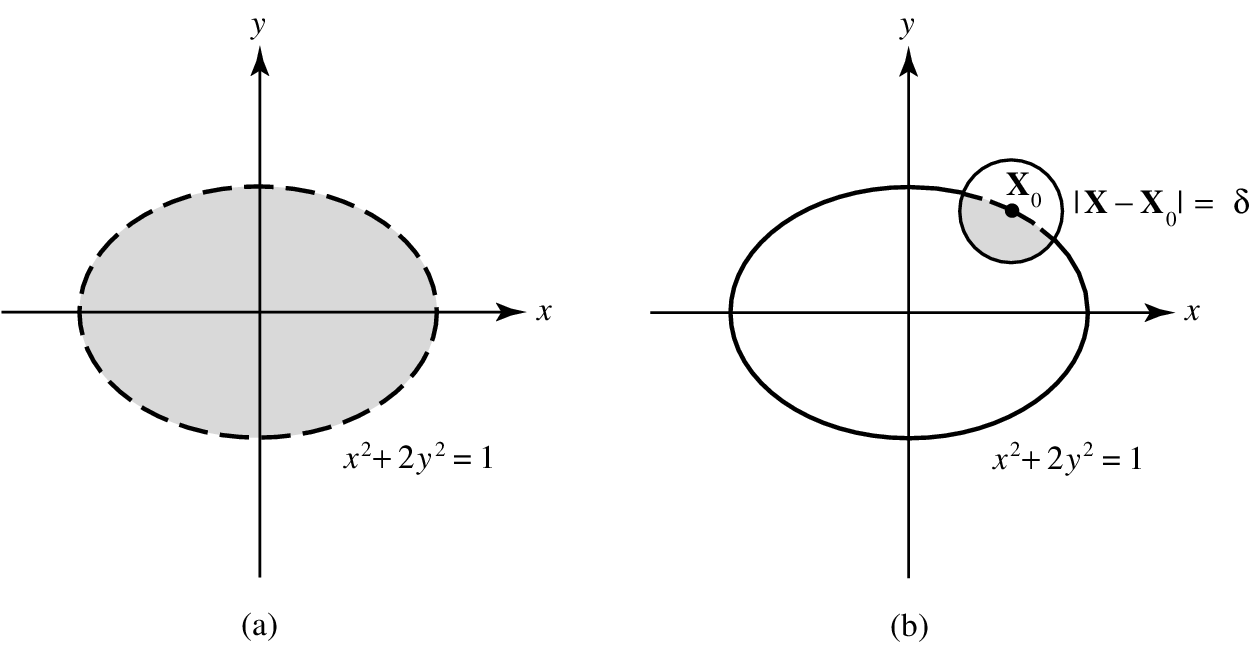
\includegraphics[width=4.2in,height=2.2in]{png/fig050201.png}
\end{center}
 \vskip6pt
 \refstepcounter{figure}
\nopagebreak
 \centerline{\bf Figure \thefigure} \label{figure:5.2.1}
\newpage

The following theorem is analogous to Theorem~2.1.3.
We leave its proof  to you
(Exercise~\ref{exer:5.2.2}).



\begin{theorem}\label{thmtype:5.2.2}
 If $\lim_{\mathbf{X}\to\mathbf{X}_0} f(\mathbf{X})$ exists$,$ then it is
unique.
\end{theorem}

When investigating whether a function has a limit at a point
$\mathbf{X}_0$, no restriction can be made on the way in which
$\mathbf{X}$
approaches $\mathbf{X}_0$, except that $\mathbf{X}$ must be in $D_f$. The next
example shows that incorrect restrictions can lead to incorrect
conclusions.

\begin{example}\label{example:5.2.3}\rm
The function
$$
f(x,y)=\frac{xy}{ x^2+y^2}
$$
is defined everywhere in $\R^2$ except at $(0,0)$. Does
$\lim_{(x,y)\to (0,0)} f(x,y)$ exist? If we try to answer this
question by letting $(x,y)$ approach $(0,0)$ along the line $y=x$, we
see the functional values
$$
f(x,x)=\frac{x^2}{2x^2}=\frac{1}{2}
$$
and conclude that the limit is $1/2$. However, if we let $(x,y)$
approach
$(0,0)$ along the line $y=-x$, we see the functional values
$$
f(x,-x)=-\frac{x^2}{2x^2}=-\frac{1}{2}
$$
and conclude that the limit equals $-1/2$. From
Theorem~\ref{thmtype:5.2.2},
these two conclusions cannot both be correct. In fact,
they are both incorrect. What we have shown is that
$$
\lim_{x\to 0} f(x,x)=\frac{1}{2}\mbox{\quad and\quad}\lim_{x\to 0}
f(x,-x)=-\frac{1}{2}.
$$
Since $\lim_{x\to 0} f(x,x)$ and $\lim_{x\to0} f(x,-x)$ must both
equal $\lim_{(x,y)\to (0,0)} f(x,y)$ if the latter exists
(Exercise~\ref{exer:5.2.3}\part{a}), we  conclude that the latter does
not exist.
\bbox\end{example}

The sum, difference, and product of functions of $n$ variables are
defined in the same way as they are for functions of one variable
(Definition~\ref{thmtype:2.1.1}), and the proof of the next
theorem is the same as the proof of
Theorem~\ref{thmtype:2.1.4}.



\enlargethispage{100pt}
\begin{theorem}\label{thmtype:5.2.3}
Suppose that  $f$ and $g$ are defined on a set $D,$ $\mathbf{X}_0$ is a
limit point of $D,$ and
$$
\lim_{\mathbf{X}\to\mathbf{X}_0} f(\mathbf{X})=L_1,\quad\lim_{\mathbf{X}\to\mathbf{X}_0} g(\mathbf{X})=L_2.
$$
Then
\begin{eqnarray}
\lim_{\mathbf{X}\to\mathbf{X}_0}(f+g)(\mathbf{X})\ar=L_1+L_2,\label{eq:5.2.10}\\
\lim_{\mathbf{X}\to\mathbf{X}_0}(f-g)(\mathbf{X})\ar=L_1-L_2,\label{eq:5.2.11}\\
\lim_{\mathbf{X}\to\mathbf{X}_0}(fg)(\mathbf{X})\ar=L_1L_2,\label{eq:5.2.12}\\
\arraytext{and$,$ if $L_2\ne0,$}\nonumber\\
\lim_{\mathbf{X}\to\mathbf{X}_0}\left(\frac{f}{ g}\right)(\mathbf{X})
\ar=\frac{L_1}{ L_2}.\label{eq:5.2.13}
\end{eqnarray}
\end{theorem}
\newpage

\boxit{Infinite Limits and Limits as ${|\mathbf{X}|
\mathbf{\mathbf{\to}\mathbf{\infty}}}$}
\vspace*{-2em}
\begin{definition}\label{thmtype:5.2.4}    \rm
We say that $f(\mathbf{X})$ {\it approaches $\infty$ as $\mathbf{X\/}$
approaches
$\mathbf{X}_0$\/} and write
$$
\lim_{\mathbf{X}\to\mathbf{X}_0} f(\mathbf{X})=\infty
$$
if $\mathbf{X}_0$ is a limit point of $D_f$ and, for every real number
$M$, there is a $\delta>0$ such that
$$
f(\mathbf{X})>M\mbox{\quad whenever\quad} 0<|\mathbf{X}-\mathbf{X}_0|<\delta
\mbox{\quad and\quad}\mathbf{X}\in D_f.
$$
We say that
\begin{eqnarray*}
\lim_{\mathbf{X}\to\mathbf{X}_0} f(\mathbf{X})\ar=-\infty\\
\arraytext{if}\\
\lim_{{\mathbf{X}}\to\mathbf{X}_0} (-f)(\mathbf{X})\ar=\infty.
\end{eqnarray*}
\end{definition}


\begin{example}\label{example:5.2.4}\rm   If
$$
f(\mathbf{X})=(1-x^2_1-x^2_2-\cdots-x^2_n)^{-1/2},
$$
then
$$
\lim_{\mathbf{X}\to\mathbf{X}_0} f(\mathbf{X})=\infty
$$
if $|\mathbf{X}_0|=1$, because
$$
f(\mathbf{X})=\frac{1}{ |\mathbf{X}-\mathbf{X}_0|},
$$
so
$$
f(\mathbf{X})>M\mbox{\quad if\quad} 0<|\mathbf{X}-\mathbf{X}_0|<\delta=\frac{1}{ M}.
$$
\end{example}

\begin{example}\label{example:5.2.5}\rm   If
$$
f(x,y)=\frac{1}{ x+2y+1},
$$
then $\lim_{(x,y)\to (1,-1)} f(x,y)$ does not exist (why not?), but
$$
\lim_{(x,y)\to (1,-1)}\left|f(x,y)\right|=\infty.
$$
To see this, we observe that
\begin{eqnarray*}
|x+2y+1|\ar=|(x-1)+2(y+1)|\\[2\jot]
\ar\le \sqrt{5}|\mathbf{X}-\mathbf{X}_0|\mbox{\quad (by Schwarz's inequality),\quad}
\end{eqnarray*}
where $\mathbf{X}_0=(1,-1)$, so
$$
|f(x,y)|=\frac{1}{ |x+2y+1|}\ge \frac{1}{\sqrt 5|\mathbf{X}-\mathbf{X}_0|}.
$$
\newpage
\noindent
Therefore,
$$
\left|f(x,y)\right|>M\mbox{\quad if\quad} 0<|\mathbf{X}-\mathbf{X}_0|<
\frac{1}{ M\sqrt{5}}.
$$
\end{example}

\begin{example}\label{example:5.2.6}\rm   The function
$$
f(x,y,z)=\frac{\left|\sin\left(\dst{\frac{1}{ x^2+y^2+z^2}}\right)
\right|}{ x^2+y^2+z^2}
$$
assumes arbitrarily large values in every neighborhood of $(0,0,0)$.
For example, if $\mathbf{X}_k=(x_k,y_k,z_k)$, where
$$
x_k=y_k=z_k=\frac{1}{\sqrt{3\left(k+\frac{1}{2}\right)\pi}},
$$
then
$$
f(\mathbf{X}_k)=\left(k+\frac{1}{2}\right)\pi.
$$
However, this does not imply that $\lim_{\mathbf{X}\to {\mathbf{0}}}
f(\mathbf{X})
=\infty$, since, for example, every neighborhood of $(0,0,0)$ also
contains points
$$
\overline{\mathbf{X}}_{k}
=\left(\frac{1}{\sqrt{3k\pi}},\frac{1}{\sqrt{3k\pi}},\frac{1}{
\sqrt{3k\pi}}\right)
$$
\noindent
for which $f(\overline{\mathbf{X}_k})=0$.
\end{example}


\begin{definition}\label{thmtype:5.2.5}       \rm
If $D_f$ is unbounded$,$ we say that
$$
\lim_{|\mathbf{X}|\to\infty} f(\mathbf{X})=L\mbox{\quad (finite)\quad}
$$
if for every $\epsilon>0$, there is a number $R$ such that
$$
|f(\mathbf{X})-L|<\epsilon\mbox{\quad whenever\quad}\ |\mathbf{X}|\ge R
\mbox{\quad and\quad}\mathbf{X}\in D_f.
$$
\end{definition}

\begin{example}\label{example:5.2.7}\rm   If
$$
f(x,y,z)=\cos\left(\frac{1}{ x^2+2y^2+z^2}\right),
$$
then
\begin{equation}\label{eq:5.2.14}
\lim_{|\mathbf{X}|\to\infty} f(\mathbf{X})=1.
\end{equation}
To see this, we recall that the continuity of $\cos u$ at $u=0$
implies that for each $\epsilon>0$ there is a $\delta>0$ such that
$$
|\cos u-1|<\epsilon\mbox{\quad if\quad} |u|<\delta.
$$
\newpage
\noindent
Since
$$
\frac{1}{ x^2+2y^2+z^2}\le \frac{1}{ |\mathbf{X}|^2},
$$
it follows that if
 $|\mathbf{X}|>1/\sqrt{\delta}$, then
$$
\frac{1}{ x^2+2y^2+z^2}<\delta.
$$
Therefore,
$$
|f(\mathbf{X})-1|<\epsilon.
$$
This proves \eqref{eq:5.2.14}.
\end{example}

\begin{example}\label{example:5.2.8}\rm Consider the function
defined
{\it only\/} on the domain
$$
D=\set{(x,y)}{0< y\le ax},\quad 0<a<1
$$
(Figure~\ref{figure:5.2.2}), by
$$
f(x,y)=\frac{1}{ x-y}.
$$
We will show that
\begin{equation} \label{eq:5.2.15}
\lim_{|\mathbf{X}|\to\infty} f(x,y)=0.
\end{equation}
It is important to keep in mind that we need only consider $(x,y)$
in $D$, since $f$ is not defined elsewhere.

In $D$,
\begin{equation}\label{eq:5.2.16}
x-y\ge x(1-a)
\end{equation}
and
$$
|\mathbf{X}|^2=x^2+y^2\le x^2(1+a^2),
$$
so
$$
x\ge \frac{|\mathbf{X}|}{\sqrt{1+a^2}}.
$$
 This and \eqref{eq:5.2.16} imply that
$$
x-y\ge \frac{1-a}{\sqrt{1+a^2}} |\mathbf{X}|,\quad\mathbf{X}\in D,
$$
so
$$
|f(x,y)|\le \frac{\sqrt{1+a^2}}{1-a} \frac{1}{ |\mathbf{X}|},\quad\mathbf{X}\in
D.
$$
Therefore,
$$
\left|f(x,y)\right|<\epsilon
$$
if $\mathbf{X}\in D$ and
$$
|\mathbf{X}|>\frac{\sqrt{1+a^2}}{1-a} \frac{1}{\epsilon}.
$$
This implies \eqref{eq:5.2.15}.
\end{example}

\topfig{-3}
\begin{center}
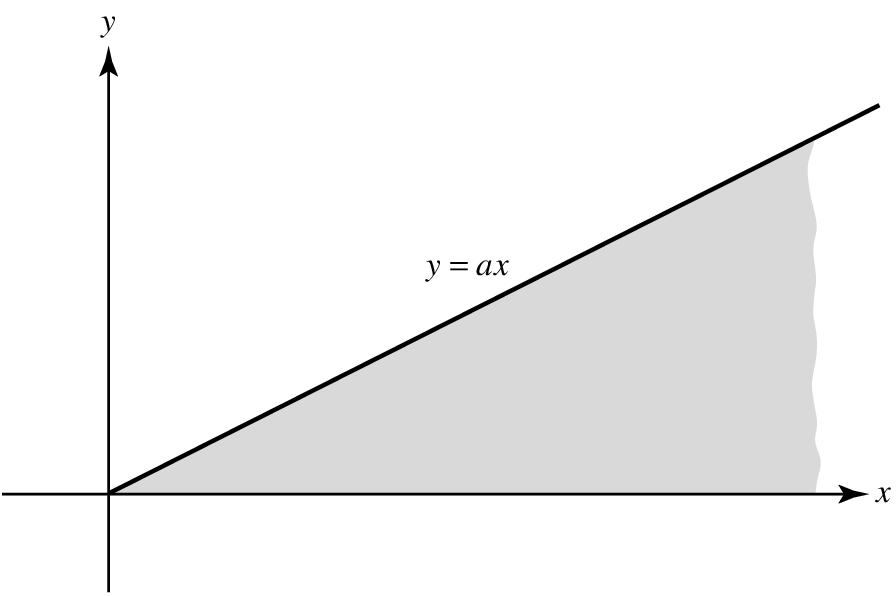
\includegraphics[width=3in,height=3in]{png/fig050202.png}
\end{center}
 \vskip6pt
 \refstepcounter{figure}
 \centerline{\bf Figure \thefigure} \label{figure:5.2.2}
 \vskip12pt

We leave it to you to define
$\lim_{|\mathbf{X}|\to\infty} f(\mathbf{X})=\infty$  and
$\lim_{|\mathbf{X}|\to\infty} f(\mathbf{X})=-\infty$
(Exercise~\ref{exer:5.2.6}).

We will continue the convention adopted in Section~2.1:
``$\lim_{\mathbf{X}\to \mathbf{X}_0} f(\mathbf{X})$ exists'' means that
$\lim_{\mathbf{X}\to\mathbf{X}_0} f(\mathbf{X})=L$, where $L$ is finite; to leave open the possibility
that $L=\pm\infty$, we will say that ``$\lim_{\mathbf{X}\to\mathbf{X}_0}
f(\mathbf{X})$
 exists in the extended reals.'' A similar convention applies to
limits as $|\mathbf{X}|\to\infty$.

Theorem~\ref{thmtype:5.2.3} remains valid if ``$\lim_{\mathbf{X}\to\mathbf{X}_0}$''
is replaced by ``$\lim_{|\mathbf{X}|\to\infty}$,'' provided that  $D$ is
unbounded.  Moreover, \eqref{eq:5.2.10},
\eqref{eq:5.2.11}, and \eqref{eq:5.2.12} are valid in either version of
Theorem~\ref{thmtype:5.2.3} if either or both of $L_1$ and $L_2$ is
infinite, provided that their right sides are not indeterminate, and
\eqref{eq:5.2.13} remains valid if $L_2\ne 0$ and $L_1/L_2$ is not
indeterminate.

\boxit{Continuity}
We now define continuity for functions of $n$ variables. The
definition is  quite similar to the definition for
functions of one variable.

\begin{definition}\label{thmtype:5.2.6} \rm
If $\mathbf{X}_0$ is in $D_f$ and is a limit point of $D_f$, then we say
that $f$ is
{\it continuous at  $\mathbf{X\/}_0$\/}  if
$$
\lim_{\mathbf{X}\to\mathbf{X}_0} f(\mathbf{X})=f(\mathbf{X}_0).
\eqno{\bbox}
$$
\end{definition}

The next theorem follows from this and
Definition~\ref{thmtype:5.2.1}.

\begin{theorem}\label{thmtype:5.2.7}
Suppose that  $\mathbf{X}_0$ is in $D_f$ and is a limit point of $D_f.$ Then
$f$
is continuous at $\mathbf{X}_0$ if and only if for each $\epsilon>0$ there
is a $\delta>0$ such that
$$
\left|f(\mathbf{X})-f(\mathbf{X}_0)\right|<\epsilon
$$
whenever
$$
|\mathbf{X}-\mathbf{X}_0|<\delta\mbox{\quad and\quad}\mathbf{X}\in D_f.
$$
\end{theorem}

In applying this theorem when $\mathbf{X}_0\in D^0_f$, we will usually
omit ``and $\mathbf{X}\in D_f$,'' it being understood that
$S_\delta (\mathbf{X}_{0}) \subset D_f$.

We will say that $f$ is {\it continuous on\/} $S$ if $f$ is continuous
at every point of $S$.

\begin{example}\label{example:5.2.9}\rm From Example~\ref{example:5.2.1}, we
now see that the function
$$
f(x,y)=1-x^2-2y^2
$$
is continuous on $\R^2$.
\end{example}

\begin{example}\label{example:5.2.10}\rm If we extend the definition of
$h$ in Example~\ref{example:5.2.2} so that
$$
h(x,y)=\left\{\casespace\begin{array}{ll}\dst\frac{\sin\sqrt{1-x^2-2y^2}}{
\sqrt{1-x^2-2y^2}},&x^2+2y^2<1,\\
 1,&x^2+2y^2=1,\end{array}\right.
$$
then it follows from Example~\ref{example:5.2.2} that $h$ is continuous on
the ellipse
$$
x^2+2y^2=1.
$$
We will see in Example~\ref{example:5.2.13} that $h$ is also
continuous on the interior of the ellipse.
\end{example}

\begin{example}\label{example:5.2.11}\rm
 It is impossible to define the
function
$$
f(x,y)=\frac{xy}{ x^2+y^2}
$$
at the origin to make it continuous there, since we saw in
Example~\ref{example:5.2.3} that
$$
\lim_{(x,y)\to (0,0)} f(x,y)
$$
does not exist.
\end{example}

Theorem~\ref{thmtype:5.2.3} implies the next theorem, which   is
analogous to Theorem~\ref{thmtype:2.2.5} and, like the
latter,  permits us to investigate continuity of a given function by
regarding the function as the result of addition, subtraction,
multiplication, and division of simpler functions.


\begin{theorem}\label{thmtype:5.2.8}
If $f$ and $g$ are continuous on a set $S$ in $\R^n,$ then so
are $f+g,$ $f-g,$ and $fg.$ Also$,$ $f/g$ is continuous at each
$\mathbf{X}_0$ in $S$ such that $g(\mathbf{X}_0)\ne0.$
\end{theorem}

\boxit{Vector-Valued Functions and Composite Functions}
Suppose that  $g_1$, $g_2$, \dots, $g_n$ are real-valued functions defined
on a subset $T$ of $\R^m$, and define the {\it vector-valued
function} $\mathbf{G}$ on $T$ by
$$
\mathbf{G}(\mathbf{U})=\left(g_1(\mathbf{U}), g_2(\mathbf{U}), \dots,
g_n(\mathbf{U})\right),\quad\mathbf{U}\in T.
$$
Then $g_1$, $g_2$, \dots, $g_n$ are the {\it component functions\/} of
$\mathbf{G}=(g_1,g_2, \dots,g_n)$. We say that
$$
\lim_{\mathbf{U}\to\mathbf{U}_0}\mathbf{G}(\mathbf{U})=\mathbf{L}=(L_1,
L_2, \dots,L_n)
$$
if
$$
\lim_{\mathbf{U}\to\mathbf{U}_0} g_i(\mathbf{U})=L_i,\quad 1\le i\le n,
$$
and that $\mathbf{G}$ is {\it continuous\/}
at
$\mathbf{U}_0$ if
$g_1$, $g_2$, \dots, $g_n$ are each continuous at $\mathbf{U}_0$.

The next theorem follows from Theorem~\ref{thmtype:5.1.14}
and Definitions~\ref{thmtype:5.2.1} and \ref{thmtype:5.2.6}. We omit the
proof.


\begin{theorem}\label{thmtype:5.2.9}
For a vector-valued function $\mathbf{G},$
$$
\lim_{\mathbf{U}\to\mathbf{U}_0}\mathbf{G}(\mathbf{U})=\mathbf{L}
$$
if and only if for each $\epsilon>0$ there is a $\delta>0$ such that
$$
|\mathbf{G}(\mathbf{U})-\mathbf{L}|<\epsilon\mbox{\quad whenever\quad}
0<|\mathbf{U}-\mathbf{U}_0|<\delta\mbox{\quad and\quad}\mathbf{U}\in D_{\mathbf{G}}.
$$
Similarly, $\mathbf{G}$ is continuous at $\mathbf{U}_0$ if and only if for
each
$\epsilon> 0$ there is a $\delta>0$ such that
$$
|\mathbf{G}(\mathbf{U})-\mathbf{G}(\mathbf{U}_0)|<\epsilon
\mbox{\quad whenever\quad}
 |\mathbf{U}-\mathbf{U}_0|<\delta\mbox{\quad and\quad}\mathbf{U}\in D_{\mathbf{G}}.
$$
\end{theorem}

The following  theorem on the continuity of a composite function is
analogous to Theorem~\ref{thmtype:2.2.7}.




\begin{theorem}\label{thmtype:5.2.10}
Let $f$ be a real-valued function defined on a subset of $\R^n,$
 and let the
vector-valued function $\mathbf{G}=(g_1,g_2, \dots,g_n)$ be defined on a
domain $D_\mathbf{G}$ in $\R^m.$ Let the set
$$
T=\set{\mathbf{U}}{\mathbf{U}\in D_{\mathbf{G}}\mbox{\quad and \quad}
\mathbf{G}(\mathbf{U})\in D_f}
$$
$($Figure~\ref{figure:5.2.3}$)$,
 be
nonempty$,$ and define the real-valued composite function
$$
h=f\circ\mathbf{G}
$$
on $T$ by
$$
h(\mathbf{U})=f(\mathbf{G}(\mathbf{U})),\quad \mathbf{U}\in T.
$$
Now suppose that  $\mathbf{U}_0$ is in $T$ and is a limit point of $T,$
$\mathbf{G}$ is continuous at $\mathbf{U}_0,$ and $f$ is continuous at
$\mathbf{X}_0=\mathbf{G}(\mathbf{U}_0).$ Then $h$ is continuous at
$\mathbf{U}_0.$
\end{theorem}
\newpage


\topfig{-3}
\begin{center}
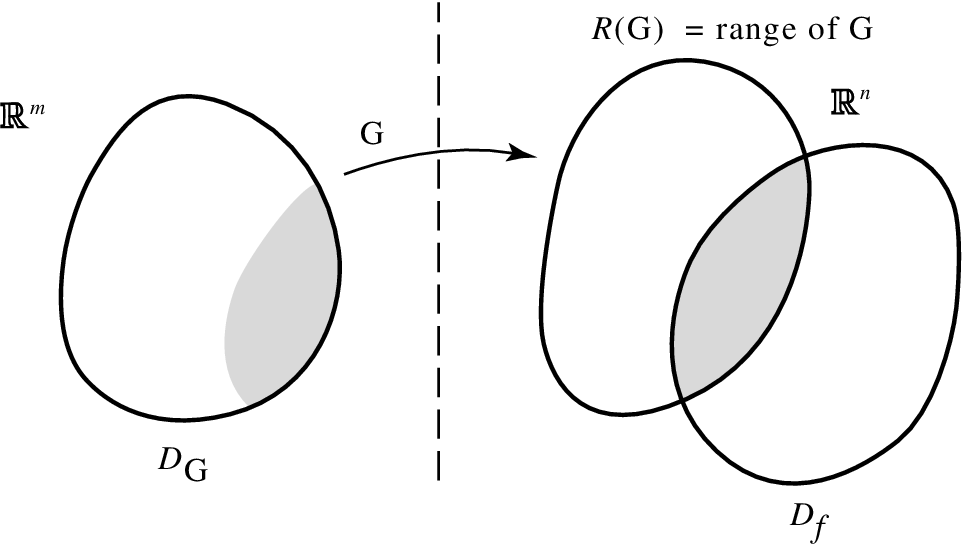
\includegraphics[width=3.25in,height=1.9in]{png/fig050203.png}
\end{center}
 \vskip6pt
 \refstepcounter{figure}
 \centerline{\bf Figure \thefigure} \label{figure:5.2.3}
 \vskip12pt

\proof
Suppose that  $\epsilon>0$. Since $f$ is continuous at
$\mathbf{X}_0=\mathbf{G}(\mathbf{U}_0)$, there is an $\epsilon_1>0$
such that
\begin{equation}\label{eq:5.2.17}
|f(\mathbf{X})-f(\mathbf{G}(\mathbf{U}_0))|<\epsilon
\end{equation}
if
\begin{equation}\label{eq:5.2.18}
|\mathbf{X}-\mathbf{G}(\mathbf{U}_0)|<\epsilon_1\mbox{\quad and\quad}
\mathbf{X}\in D_f.
\end{equation}
Since $\mathbf{G}$ is continuous at $\mathbf{U}_0$, there is a $\delta>0$
such that
$$
|\mathbf{G}(\mathbf{U})-\mathbf{G}(\mathbf{U}_0)|<\epsilon_1
\mbox{\quad if\quad} |\mathbf{U}-\mathbf{U}_0|<
\delta\mbox{\quad and\quad}\mathbf{U}\in D_\mathbf{G}.
$$
By taking $\mathbf{X}=\mathbf{G}(\mathbf{U})$ in \eqref{eq:5.2.17} and
\eqref{eq:5.2.18}, we see that
$$
|h(\mathbf{U})-h(\mathbf{U}_0)|=|f(\mathbf{G}(\mathbf{U})
-f(\mathbf{G}(\mathbf{U}_0))|<\epsilon
$$
if
$$
|\mathbf{U}-\mathbf{U}_0|<\delta\mbox{\quad and\quad}\mathbf{U}\in T.
$$
\bbox

\begin{example}\label{example:5.2.12}\rm   If
$$
f(s)=\sqrt{s}
$$
 and
$$
g(x,y)=1-x^2-2y^2,
$$
then $D_f=[0,\infty]$, $D_g=\R^2$, and
$$
T=\set{(x,y)}{x^2+2y^2\le1}.
$$
From Theorem~\ref{thmtype:5.2.7} and
Example~\ref{example:5.2.1},
 $g$ is continuous on $\R^2$. (We can obtain the same
conclusion by observing that the functions $p_1(x,y)=x$ and
$p_2(x,y)=y$
are continuous on $\R^2$ and applying Theorem~\ref{thmtype:5.2.8}.)
Since $f$ is continuous on $D_f$, the function
$$
h(x,y)=f\left(g(x,y)\right)=\sqrt{1-x^2-2y^2}
$$
is continuous on $T$.
\end{example}


\begin{example}\label{example:5.2.13}\rm   If
$$
g(x,y)=\sqrt{1-x^2-2y^2}
$$
and
$$
f(s)=\left\{\casespace\begin{array}{ll} {\dst{\frac{\sin s}{ s}}},&s\ne0,\\[2\jot]
 1,&s=0,\end{array}\right.
$$
then $D_f=(-\infty,\infty)$ and
$$
D_g=T=\set{(x,y)}{x^2+2y^2\le1}.
$$
In Example~\ref{example:5.2.12} we saw that $g$ (we called it $h$ there)
is continuous on $T$. Since $f$ is continuous on $D_f$, the composite
function $h=f\circ g$ defined by
$$
h(x,y)=\left\{\casespace\begin{array}{ll}\dst{\frac{\sin\sqrt{1-x^2-2y^2}}{
\sqrt{1-x^2-2y^2}}},&x^2+2y^2<1,\\[2\jot]
 1,&x^2+2y^2=1,\end{array}\right.
$$
is continuous on $T$.  This implies the result of Example~\ref{example:5.2.2}.
\end{example}

\boxit{Bounded Functions}
\hskip-.4em
The definitions of {\it bounded above, bounded below\/}, and {\it bounded\/}
on a set $S$ are the same for functions of $n$ variables as for functions
of one variable, as are the definitions of {\it supremum\/} and {\it
infimum\/}
of a function on a set $S$ (Section 2.2).  The
proofs of the next two theorems are similar to those of
Theorems~\ref{thmtype:2.2.8} and \ref{thmtype:2.2.9}
(Exercises~\ref{exer:5.2.12}  and \ref{exer:5.2.13}).

\begin{theorem}\label{thmtype:5.2.11}
If $f$ is continuous on a compact set $S$ in $\R^n,$ then $f$
is bounded on~$S.$
\end{theorem}

\begin{theorem}\label{thmtype:5.2.12}
Let $f$ be continuous on a compact set $S$ in $\R^n$ and
$$
\alpha=\inf_{\mathbf{X}\in S}f(\mathbf{X}),\quad\beta=
\sup_{\mathbf{X}\in S}f(\mathbf{X}).
$$
Then
$$
f(\mathbf{X}_1)=\alpha\mbox{\quad and\quad} f(\mathbf{X}_2)=\beta
$$
for some $\mathbf{X}_1$ and $\mathbf{X}_2$ in $S.$
\end{theorem}

The next theorem is analogous to  Theorem~\ref{thmtype:2.2.10}.



\begin{theorem} [Intermediate Value Theorem]\label{thmtype:5.2.13}
Let $f$ be continuous on a region $S$ in $\R^n.$ Suppose that
$\mathbf{A}$ and $\mathbf{B}$ are in $S$ and
$$
f(\mathbf{A})<u<f(\mathbf{B}).
$$
Then $f(\mathbf{C})=u$ for some $\mathbf{C}$ in $S.$
\end{theorem}
\newpage

\proof
If there is no such $\mathbf{C}$, then $S=R\cup T$, where
\begin{eqnarray*}
R\ar=\set{\mathbf{X}}{\mathbf{X}\in S\mbox{ and } f(\mathbf{X})<u}\\
\arraytext{and}\\
T\ar=\set{\mathbf{X}}{\mathbf{X}\in S\mbox{ and } f(\mathbf{X})>u}.
\end{eqnarray*}
If $\mathbf{X}_0\in R$, the continuity of $f$ implies that there is a
$\delta>0$ such that $f(\mathbf{X})<u$ if $|\mathbf{X}-\mathbf{X}_0|<\delta$
and $\mathbf{X}\in S$. This means that $\mathbf{X}_0\not\in\overline{T}$.
Therefore, $R\cap\overline{T}=\emptyset$. Similarly, $\overline{R}\cap
T=\emptyset$. Therefore, $S$ is disconnected
(Definition~\ref{thmtype:5.1.19}), which contradicts the
assumption that $S$ is a region (Exercise~\ref{exer:5.1.30}).
Hence, we conclude that $f(\mathbf{C})=u$ for some $\mathbf{C}$ in $S$.
\bbox

\boxit{Uniform Continuity}
\hskip-.4em
The definition of uniform continuity for functions of $n$
variables is the same as  for functions of one variable; $f$ is
uniformly
continuous on a subset $S$ of its domain in $\R^n$ if for every
$\epsilon>0$ there is a $\delta>0$ such that
$$
|f(\mathbf{X})-f(\mathbf{X}')|<\epsilon
$$
whenever $|\mathbf{X}-\mathbf{X}'|<\delta$ and $\mathbf{X},\mathbf{X}'\in S$. We
emphasize again that $\delta$ must depend only on $\epsilon$ and $S$,
and not on the particular points $\mathbf{X}$ and $\mathbf{X}'$.

The proof of the next theorem is analogous to that of
Theorem~\ref{thmtype:2.2.12}. We leave it to you
(Exercise~\ref{exer:5.2.14}).

\begin{theorem}\label{thmtype:5.2.14}
If $f$ is continuous on a compact set $S$ in $\R^n,$ then $f$
is uniformly continuous on $S.$
\end{theorem}

\exercises


\noindent{\it
With $\R$ replaced by $\R^n,$ the following exercises
from Sections~$2.1$ and $2.2$ have analogs for this
section:
$\ref{exer:2.1.5}$,
$\ref{exer:2.1.8}$--$\ref{exer:2.1.11}$,
$\ref{exer:2.1.26}$,
$\ref{exer:2.1.28}$,
$\ref{exer:2.1.29}$,
$\ref{exer:2.1.33}$,
$\ref{exer:2.2.8},$
$\ref{exer:2.2.9},$
$\ref{exer:2.2.10}$,
$\ref{exer:2.2.15}$,
$\ref{exer:2.2.16}$,
$\ref{exer:2.2.20}$,
$\ref{exer:2.2.29}$,
$\ref{exer:2.2.30}$. }

\begin{exerciselist}


\item\label{exer:5.2.1}  Find $\lim_{\mathbf{X}\to\mathbf{X}_0}f(\mathbf{X})$ and
justify your
answer with an $\epsilon$--$\delta$ argument, as required by
Definition~\ref{thmtype:5.2.1}. \hint{See Examples~$\ref{example:5.2.1}$ and
$\ref{example:5.2.2}.$}
\begin{alist}
\item % (a)
 $f(\mathbf{X})=3x+4y+z-2$,\quad $\mathbf{X}_0=(1,2,1)$\\
\item % (b)
 $\dst{f(\mathbf{X})=\frac{x^3-y^3}{ x-y}}$,\quad $\mathbf{X}_0=(1,1)$\\
\item % (c)
 $\dst{f(\mathbf{X})=\frac{\sin(x+4y+2z)}{ x+4y+2z}}$,\quad
$\mathbf{X}_0=(-2,1,-1)$
\newpage

\item % (d)
 $f(\mathbf{X})=(x^2+y^2)\log(x^2+y^2)^{1/2}$,\quad $\mathbf{X}_0=(0,
0)$\\
\item % (e)
 $\dst{f(\mathbf{X})=\frac{\sin(x-y)}{\sqrt{x-y}}}$, \quad
$\mathbf{X}_0=(2,2)$\\
\item % (f)
 $\dst{f(\mathbf{X})=\frac{1}{ |\mathbf{X}|}e^{-1/|\mathbf{X}|}}$,
\quad $\mathbf{X}_0=\mathbf{0}$\\
\end{alist}


\item\label{exer:5.2.2} Prove Theorem~\ref{thmtype:5.2.2}.

\item\label{exer:5.2.3} If $\lim_{x\to x_0}y(x)=y_0$ and $\lim_{x\to
x_0}f\left(x,y(x)\right)=L$, we say that $f(x,y)$ {\it approaches $L$
as $(x,y)$ approaches $(x_0,y_0)$ along the curve $y=y(x)$}.
\begin{alist}
\item % (a)
 Prove:  If $\lim_{(x,y)\to (x_0,y_0)}f(x,y)=L$, then
$f(x,y)$ approaches $L$ as $(x,y)$ approaches $(x_0,y_0)$ along any curve
$y=y(x)$ through $(x_0,y_0)$.
\item % (b)
 We saw in Example~\ref{example:5.2.3} that if
$$
f(x,y)=\frac{xy}{ x^2+y^2},
$$
then $\lim_{(x,y)\to(0,0)} f(x,y)$ does not exist. Show, however, that
$f(x,y)$ approaches a value $L_a$ as $(x,y)$ approaches $(0,0)$ along
any curve $y=y(x)$ that passes through $(0,0)$ with slope $a$. Find
$L_a$.
\item % (c)
Show that the function
$$
g(x,y)=\frac{x^3y^4}{(x^2+y^6)^3}
$$
approaches $0$ as $(x,y)$ approaches $(0,0)$ along a curve as described in
\part{b}, but that $\lim_{(x,y)\to (0,0)}f(x,y)$ does not exist.
\end{alist}


\item\label{exer:5.2.4} Determine
whether $\lim_{\mathbf{X}\to\mathbf{X}_0} f(\mathbf{X})=\pm\infty$.
\begin{alist}
\item % (a)
 $\dst{f(\mathbf{X})=\frac{|\sin(x+2y+4z)|}{
(x+2y+4z)^2}}$,\quad $\mathbf{X}_0=(2,-1,0)$\\
\item % (b)
 $\dst{f(\mathbf{X})=\frac{1}{\sqrt{x-y}}}$,\quad $\mathbf{X}_0=(0,0)$\\
\item % (c)
 $\dst{f(\mathbf{X})=\frac{\sin1/x}{\sqrt{x-y}}}$,\quad
$\mathbf{X}_0=(0,0)$\\
\item % (d)
$\dst{f(\mathbf{X})=\frac{4y^2-x^2}{(x-2y)^3}}$,\quad
$\mathbf{X}_0=(2,1)$\\
\item % (e)
 $\dst{f(\mathbf{X})=\frac{\sin(x+2y+4z)}{
(x+2y+4z)^2}}$,\quad $\mathbf{X}_0=(2,-1,0)$
\end{alist}

\item\label{exer:5.2.5}
 Find $\lim_{|\mathbf{X}|\to\infty} f(\mathbf{X})$, if it
exists.

\begin{tabular}[t]{@{}p{168pt}@{}p{168pt}}
\part{a} $\dst{f(\mathbf{X})=\frac{\log(x^2+2y^2+4z^2)}{
x^2+y^2+z^2}}$&
\part{b} $\dst{f(\mathbf{X})=\frac{\sin(x^2+y^2)}{\sqrt{x^2+y^2}}}$\\\\
\part{c} $f(\mathbf{X})=e^{-(x+y)^2}$ &
\part{d} $f(\mathbf{X})=e^{-x^2-y^2}$
\end{tabular}

\part{e} $f(\mathbf{X})=\left\{\casespace\begin{array}{ll}
\dst\frac{\sin(x^2-y^2)}{ x^2-y^2},&x\ne\pm y,\\[2\jot]
 1,&x=\pm y\end{array}\right.$


\item\label{exer:5.2.6}
Define
\part{a}
 $\lim_{|\mathbf{X}|\to\infty} f(\mathbf{X})=\infty$ and
\part{b} $\lim_{|\mathbf{X}|\to\infty}f(\mathbf{X})=-\infty$.

\item\label{exer:5.2.7} Let
$$
f(\mathbf{X})=\frac{|x_1|^{a_1} |x_2|^{a_2}\cdots
|x_n|^{a_n}}{\mathbf{X}|^b}.
$$
For what nonnegative values of  $a_1$, $a_2$, \dots, $a_n$, $b$ does
$\lim_{\mathbf{X}\to\mathbf{0}}f(\mathbf{X})$  exist in the extended reals?

\item\label{exer:5.2.8} Let
$$
g(\mathbf{X})=\frac{(x^2+y^4)^3}{1+x^6y^4}.
$$
Show that $\lim_{|x|\to\infty}g(x,ax)=\infty$ for any real number $a$.
Does
$$
\lim_{|\mathbf{X}|\to\infty} g(\mathbf{X})=\infty?
$$





\item\label{exer:5.2.9} For each $f$ in Exercise~\ref{exer:5.2.1}, find the
largest set $S$ on which $f$ is continuous or can be defined so as to
be continuous.

\item\label{exer:5.2.10} Repeat Exercise~\ref{exer:5.2.9} for the functions
in Exercise~\ref{exer:5.2.5}.

\item\label{exer:5.2.11} Give an example of a function $f$ on $\R^2$
such that $f$ is not continuous at $(0,0)$, but $f(0,y)$ is a
continuous function of $y$ on $(-\infty,\infty)$ and $f(x,0)$ is a
continuous function of $x$ on $(-\infty,\infty)$.

\item\label{exer:5.2.12} Prove Theorem~\ref{thmtype:5.2.11}. \hint{See the
proof of Theorem~$\ref{thmtype:2.2.8}.$}

\item\label{exer:5.2.13} Prove Theorem~\ref{thmtype:5.2.12}. \hint{See the
proof of Theorem~$\ref{thmtype:2.2.9}.$}

\item\label{exer:5.2.14} Prove Theorem~\ref{thmtype:5.2.14}. \hint{See the
proof of Theorem~$\ref{thmtype:2.2.12}.$}

\item\label{exer:5.2.15}
Suppose that  $\overline{\mathbf{X}}\in D_f\subset
\R^n$ and $\overline{\mathbf{X}}$ is a limit point of $D_f$. Show
that $f$ is continuous at $\overline{\mathbf{X}}$ if and only if
$\lim_{k\to\infty}f(\mathbf{X}_k)=f(\overline{\mathbf{X}})$ whenever
$\{\mathbf{X}_k\}$
 is a sequence of points in $D_f$ such that
$\lim_{k\to\infty}\mathbf{X}_k=\overline{\mathbf{X}}$. \hint{See the proof of
Theorem~$\ref{thmtype:4.2.6}.$}


\label{sectionend:\thesection} \end{exerciselist}

\currentpdfbookmark{Section 5.3 Partial Derivatives and the
Differential}{section:5.3}
\newsection{3}
{Real-Valued Functions of Several Variables}
{Partial Derivatives and the Differential}


\renewcommand{\thissection}{\sectiontitle {PARTIAL DERIVATIVES AND THE
DIFFERENTIAL}} \thissection

\noindent
To say that a function of one variable has a derivative at $x_0$ is
the same as to say that it is differentiable at $x_0$. The situation
is not so simple for a function $f$ of more than one variable. First,
there
is no specific number that can be called {\it the\/} derivative of $f$
at a point $\mathbf{X}_0$ in $\R^n$. In fact, there are infinitely
many numbers, called the {\it directional derivatives of $f$ at\/}
$\mathbf{X}_0$ (defined below),
that are analogous to the derivative of a
function of one variable.
Second, we will see that the existence of directional derivatives at
$\mathbf{X}_0$ does not imply that $f$ is differentiable at $\mathbf{X}_0$, if
differentiability at $\mathbf{X}_0$ is to imply (as it does for functions
of one variable) that $f(\mathbf{X})-f(\mathbf{X}_0)$ can be approximated
well near $\mathbf{X}_0$ by a simple linear function, or even that $f$ is
continuous at $\mathbf{X}_0$.

We will now define directional derivatives and partial derivatives of
functions
of several variables. However, we will still have occasion to refer to
derivatives of functions of one variable. We will call them
{\it ordinary\/} derivatives when we wish to distinguish between them
and the partial derivatives that we are about to define.

\begin{definition}\label{thmtype:5.3.1}
Let $\boldsymbol{\Phi}$ be a unit vector and $\mathbf{X}$ a point in
$\R^n$.
 {\it The directional derivative of $f$ at $\mathbf{X}$ in the
direction of\/} $\boldsymbol{\Phi}$ is defined by
$$
\frac{\partial f(\mathbf{X})}{\partial\boldsymbol{\Phi}}=\lim_{t\to
0}\frac
{f(\mathbf{X}+ t\boldsymbol{\Phi})-f(\mathbf{X})}{ t}
$$
if the limit exists. That is, $\partial f(\mathbf{X})/\partial\boldsymbol{\Phi}$
is the ordinary derivative of the function
$$
h(t)=f(\mathbf{X}+t\boldsymbol{\Phi})
$$
at $t=0$, if $h'(0)$ exists.
\end{definition}

\begin{example}\label{example:5.3.1}\rm Let
$\boldsymbol{\Phi}=(\phi_1,\phi_2,\phi_3)$ and
$$
f(x,y,z)=3xyz+2x^2+z^2.
$$
Then
\begin{eqnarray*}
h(t)\ar=f(x+t\phi_1,y+t\phi_2,z+t\phi_3),\\
\ar=3(x+t\phi_1)(y+t\phi_2)(z+t\phi_3)+2(x+t\phi_1)^2+(z+t\phi_3)^2
\end{eqnarray*}
and
\begin{eqnarray*}
h'(t)\ar=3\phi_1(y+t\phi_2)(z+t\phi_3)+3\phi_2(x+t\phi_1)(z+t\phi_3)\\
\ar{}+\,3\phi_3(x+t\phi_1)(y+t\phi_2)+4\phi_1(x+t\phi_1)+
2\phi_3(z+t\phi_3).
\end{eqnarray*}
Therefore,
\hskip2pc
\begin{equation}\label{eq:5.3.1}
\frac{\partial f(\mathbf{X})}{\partial\boldsymbol{\Phi}}=h'(0)=(3yz+4x)\phi_1+
3xz\phi_2+(3xy+2z)\phi_3.
\end{equation}
\end{example}
\vskip-2em\bbox\vskip2em

The directional derivatives that we are most interested in are those in the
directions of the unit vectors
$$
\mathbf{E}_1=(1,0, \dots,0),\quad\mathbf{E}_2=(0,1,0, \dots,0),
\dots,\quad
\mathbf{E}_n=(0, \dots,0,1).
$$
(All components of $\mathbf{E}_i$ are zero except for the $i$th, which is
$1$.) Since $\mathbf{X}$ and $\mathbf{X}+t\mathbf{E}_i$ differ only in the
$i$th
coordinate, $\partial f(\mathbf{X})/\partial\mathbf{E}_i$ is called the {\it
partial derivative of $f$ with respect to $x_i$ at $\mathbf{X}$}. It is
also denoted by $\partial f(\mathbf{X})/\partial x_i$ or
$f_{x_i}(\mathbf{X})$; thus,
$$
\frac{\partial f(\mathbf{X})}{\partial x_1}=f_{x_1}(\mathbf{X})=\lim_{t\to
0} \frac{f(x_1+t, x_2, \dots,x_n)-f(x_1,x_2, \dots,x_n)}{ t},
$$
\newpage
$$
\frac{\partial f(\mathbf{X})}{\partial x_i}=f_{x_i}(\mathbf{X})=
\lim_{t\to0}
\frac{{f(x_1, \dots, x_{i-1}, x_i+t,
x_{i+1}, \dots, x_n)}
-f(x_1,x_2, \dots,x_n)
}{ t}
$$
if $2\le i\le n$,  and
$$
\frac{\partial f(\mathbf{X})}{\partial x_n}=f_{x_n}(\mathbf{X})=\lim_{t\to
0} \frac{f(x_1, \dots,x_{n-1},x_n+t)-f(x_1, \dots,x_{n-1},x_n)}{ t},
$$
if the limits exist.

If we write $\mathbf{X}=(x,y)$, then we denote the partial derivatives
accordingly; thus,
\begin{eqnarray*}
\frac{\partial f(x,y)}{\partial x}\ar=f_x(x,y)=\lim_{h\to 0}
\frac{f(x+h,y)- f(x,y)}{ h}\\
\arraytext{and}\\
\frac{\partial f(x,y)}{\partial y}\ar=f_y(x,y)=\lim_{h\to 0}
\frac{f(x,y+h)- f(x,y)}{ h}.
\end{eqnarray*}

It can be seen from these definitions that to compute
 $f_{x_i}(\mathbf{X})$
 we simply differentiate $f$ with respect to $x_i$ according to
the rules for ordinary differentiation, while treating the other
variables as constants.

\hskip1pc
\begin{example}\label{example:5.3.2}\rm   Let
\begin{equation}\label{eq:5.3.2}
f(x,y,z)=3xyz+2x^2+z^2
\end{equation}
as in Example~\ref{example:5.3.1}. Taking
 $\boldsymbol{\Phi}=\mathbf{E}_1$ (that is,
setting $\phi_1=1$ and $\phi_2=\phi_3=0$) in \eqref{eq:5.3.1}, we find
that
$$
\frac{\partial f(\mathbf{X})}{\partial x}=\frac{\partial f(\mathbf{X})}{\partial\mathbf{E}_1}=
3yz+4x,
$$
which is the result obtained by regarding $y$ and $z$ as constants in
\eqref{eq:5.3.2} and taking the ordinary derivative with respect to $x$.
Similarly,
\begin{eqnarray*}
\frac{\partial f(\mathbf{X})}{\partial y}\ar=\frac{\partial
f(\mathbf{X})}{\partial\mathbf{E}_2}=3xz\\
\arraytext{and}\\
\frac{\partial f(\mathbf{X})}{\partial z}\ar=\frac{\partial f(\mathbf{X})
}{\partial\mathbf{E}_3}=3xy+2z.
\end{eqnarray*}
\end{example}
\vskip-3em\bbox\vskip3em

The next theorem follows from the rule just given for calculating
partial derivatives.

\begin{theorem}\label{thmtype:5.3.2}
If $f_{x_i} (\mathbf{X})$ and $g_{x_i} (\mathbf{X})$ exist$,$ then
\begin{eqnarray*}
\frac{\partial (f+g)(\mathbf{X})}{\partial x_i}\ar=f_{x_i}(\mathbf{X})+
g_{x_i}(\mathbf{X}),\\
\frac{\partial (fg)(\mathbf{X})}{\partial x_i}\ar=f_{x_i}(\mathbf{X})
g(\mathbf{X})+f(\mathbf{X})g_{x_i} (\mathbf{X}),
\end{eqnarray*}
\newpage
\noindent
and$,$ if $g(\mathbf{X})\ne0,$
$$
\frac{\partial (f/g)(\mathbf{X})}{\partial x_i}=\frac{g(\mathbf{X})f_{x_i}
(\mathbf{X})- f(\mathbf{X})g_{x_i}(\mathbf{X})}{[g(\mathbf{X})]^2}.
$$
\end{theorem}

If $f_{x_i}(\mathbf{X})$ exists at every point of a set $D$, then it
defines a function $f_{x_i}$ on $D$. If this function has a partial
derivative with respect to $x_j$ on a subset of $D$, we denote the
partial derivative  by
$$
\frac{\partial}{\partial x_j}\left(\frac{\partial f}{\partial x_{i}}
\right)=\frac{\partial^2 f}{\partial x_j\partial x_i}=f_{x_ix_j}.
$$
Similarly,
$$
\frac{\partial}{\partial x_k}\left(\frac{\partial^2 f}{\partial x_j
\partial x_i}\right)=\frac{\partial^3 f}{\partial x_k\partial x_j
\partial x_i}=f_{x_ix_jx_k}.
$$
The function obtained by differentiating $f$ successively with respect
to $x_{i_1}, x_{i_2}, \dots, x_{i_r}$ is denoted by
$$
\frac{\partial^r f}{\partial x_{i_r}\partial x_{i_{r-1}}\cdots\partial
x_{i1}}=f_{x_{i_1}}\cdots x_{i_{r-1}} x_{i_r};
$$
it is  an {\it $r$th-order partial derivative of $f$\/}.

\begin{example}\label{example:5.3.3}\rm   The function
$$
f(x,y)=3x^2y^3+xy
$$
has partial derivatives everywhere. Its first-order partial
derivatives are
$$
f_x(x,y)=6xy^3+y,\quad f_y(x,y)=9x^2y^2+x.
$$
Its second-order partial derivatives are
$$
\begin{array}{rclrcl}
f_{xx}(x,y)\ar=6y^3, &f_{yy}(x,y)\ar=18x^2y,\\
f_{xy}(x,y)\ar=18 xy^2+1,&f_{yx}(x,y)\ar=18xy^2+1.
\end{array}
$$
There are eight third-order partial derivatives. Some examples are
$$
f_{xxy}(x,y)=18y^2,\quad f_{xyx}(x,y)=18y^2,\quad f_{yxx}(x,y)=
18y^2.
$$
\end{example}

\begin{example}\label{example:5.3.4}\rm Compute $f_{xx}(0,0)$,
$f_{yy}(0,0)$, $f_{xy}(0,0)$, and $f_{yx}(0,0)$ if
$$
f(x,y)=\left\{\casespace\begin{array}{ll}
\dst\frac{(x^2y+xy^2)\sin(x-y)}{ x^2+y^2},&
(x,y)\ne (0,0),\\
 0,&(x,y)=(0,0).\end{array}\right.
$$

\solution
If $(x,y)\ne(0,0)$,
the ordinary rules for differentiation, applied separately to $x$ and
$y$, yield
\begin{equation}\label{eq:5.3.3}
\begin{array}{rcl}
f_x(x,y)\ar=\dst\frac{(2xy+y^2)\sin(x-y)+(x^2y+xy^2)\cos(x-y)}{
x^2+y^2}\\[2\jot]
\ar{}-\dst\frac{2x(x^2y+xy^2)\sin(x-y)}{(x^2+y^2)^2},\quad
(x,y)\ne
(0,0),
\end{array}
\end{equation}
\newpage
\noindent
and
\begin{equation} \label{eq:5.3.4}
\begin{array}{rcl}
f_y(x,y)\ar=\dst\frac{(x^2+2xy)\sin(x-y)-(x^2y+xy^2)\cos(x-y)}{
x^2+y^2}\\[2\jot]
\ar{}-\dst\frac{2y(x^2y+xy^2)\sin(x-y)}{(x^2+y^2)^2},\quad
(x,y)\ne
(0,0).
\end{array}
\end{equation}
These formulas do not apply if
$(x,y)=(0,0)$, so we find $f_x(0,0)$ and $f_y(0,0)$ from their
definitions as difference quotients:
\begin{eqnarray*}
f_x(0,0)\ar=\lim_{x\to 0}\frac{f(x,0)-f(0,0)}{ x}=\lim_{x\to 0}
\frac{0-0}{ x}=0,\\[2\jot]
f_y(0,0)\ar=\lim_{y\to 0}\frac{f(0,y)-f(0,0)}{ y}=\lim_{y\to
0}\frac{0-0}{ y}=0.
\end{eqnarray*}
Setting $y=0$ in \eqref{eq:5.3.3} and \eqref{eq:5.3.4} yields
$$
f_x(x,0)=0,\quad f_y(x,0)=\sin x,\quad x\ne0,
$$
 so
\begin{eqnarray*}
f_{xx}(0,0)\ar=\lim_{x\to 0}\frac{f_x(x,0)-f_x(0,0)}{ x}=\lim_{x\to 0}
\frac{0-0}{ x}=0,\\[2\jot]
f_{yx}(0,0)\ar=\lim_{x\to 0}\frac{f_y(x,0)-f_y(0,0)}{ x}=\lim_{x\to 0}
\frac{\sin x-0}{ x}=1.
\end{eqnarray*}
Setting $x=0$ in \eqref{eq:5.3.3} and \eqref{eq:5.3.4} yields
$$
f_x(0,y)=-\sin y,\quad f_y(0,y)=0,\quad y\ne0,
$$
so
\begin{eqnarray*}
f_{xy}(0,0)\ar=\lim_{y\to 0}\frac{f_x(0,y)-f_x(0,0)}{ y}=\lim_{y\to 0}
\frac{-\sin y-0}{ y}=-1,\\[2\jot]
f_{yy}(0,0)\ar=\lim_{y\to 0}\frac{f_y(0,y)-f_y(0,0)}{ y}=\lim_{y\to 0}
\frac{0-0}{ y}=0.
\end{eqnarray*}
\end{example}
\vspace*{-9ex}\bbox\vspace*{6ex}

This example shows that $f_{xy}(\mathbf{X}_0)$ and $f_{yx}(\mathbf{X}_0)$ may
differ. However, the next theorem shows that they are equal if $f$
satisfies a fairly mild condition.

\begin{theorem}\label{thmtype:5.3.3}
Suppose that  $f,$ $f_x,$ $f_y,$ and $f_{xy}$ exist on a neighborhood
$N$ of $(x_0,y_0),$ and $f_{xy}$ is continuous at $(x_0,y_0).$ Then
$f_{yx}(x_0,y_0)$ exists, and
\begin{equation}\label{eq:5.3.5}
f_{yx}(x_0,y_0)=f_{xy}(x_0,y_0).
\end{equation}
\end{theorem}
\nopagebreak

\proof
 Suppose that  $\epsilon>0$.  Choose $\delta>0$ so that
the open square
\newpage
$$
S_\delta=\set{(x,y)}{|x-x_0|<\delta, |y-y_0|<\delta}
$$
is in $N$ and
\begin{equation}\label{eq:5.3.6}
|f_{xy}(\widehat{x},\widehat{y})-f_{xy}(x_0,y_0)|<\epsilon\quad
\mbox{\quad if\quad}(\widehat{x},\widehat{y})\in S_\delta.
\end{equation}
This is possible because of the continuity of $f_{xy}$ at $(x_0,y_0)$.
The function
\begin{equation}\label{eq:5.3.7}
A(h,k)=f(x_0+h, y_0+k)-f(x_0+h,y_0)-f(x_0,y_0+k)+f(x_0,y_0)
\end{equation}
is defined if $-\delta<h$, $k<\delta$; moreover,
\begin{equation}\label{eq:5.3.8}
A(h,k)=\phi(x_0+h)-\phi(x_0),
\end{equation}
where
$$
\phi(x)=f(x,y_0+k)-f(x,y_0).
$$
Since
$$
\phi'(x)=f_x(x,y_0+k)-f_x(x,y_0),\quad |x-x_0|<\delta,
$$
\eqref{eq:5.3.8} and the mean value theorem imply that
\begin{equation}\label{eq:5.3.9}
A(h,k)=\left[f_x (\widehat{x},y_0+k)-f_x(\widehat{x},y_0)\right]h,
\end{equation}
where $\widehat{x}$ is between $x_0$ and $x_0+h$. The mean value theorem,
applied to $f_x(\widehat{x},y)$ (where $\widehat{x}$ is regarded as constant),
also implies that
$$
f_x(\widehat{x},y_0+k)-f_x(\widehat{x},y_0)=f_{xy}(\widehat{x},\widehat{y})k,
$$
where $\widehat{y}$ is between $y_0$ and $y_0+k$.  From this and \eqref{eq:5.3.9},
$$
A(h,k)=f_{xy}(\widehat{x},\widehat{y})hk.
$$
Now \eqref{eq:5.3.6} implies that
\begin{equation}\label{eq:5.3.10}
\left|\frac{A(h,k)}{ hk}-f_{xy}(x_0,y_0)\right|=\left|f_{xy}(\widehat{x},
\widehat{y})-f_{xy}(x_0,y_0)\right|<\epsilon
\mbox{\quad if\quad} 0<|h|, |k|<\delta.
\end{equation}
Since \eqref{eq:5.3.7} implies that
\begin{eqnarray*}
\lim_{k\to 0}\frac{A(h,k)}{ hk}\ar=\lim_{k\to 0}
\frac{f(x_0+h,y_0+k)-f(x_0
+h,y_0)}{ hk}\\
\ar{}-\lim_{k\to 0}\frac{f(x_0,y_0+k)-f(x_0,y_0)}{ hk}\\
\ar=\frac{f_y(x_0+h,y_0)-f_y(x_0,y_0)}{ h},
\end{eqnarray*}
it follows from \eqref{eq:5.3.10} that
$$
\left|\frac{f_y(x_0+h,y_0)-f_y(x_0,y_0)}{ h}-f_{xy}(x_0,y_0)\right|\le
\epsilon\mbox{\quad if\quad} 0<|h|<\delta.
$$
\newpage
\noindent
Taking the limit as $h\to0$ yields
$$
|f_{yx}(x_0,y_0)-f_{xy}(x_0,y_0)|\le\epsilon.
$$
Since $\epsilon$ is an arbitrary positive number,
this proves \eqref{eq:5.3.5}.
\bbox

Theorem~\ref{thmtype:5.3.3}
implies the following theorem. We leave the proof to you
(Exercises~\ref{exer:5.3.10} and \ref{exer:5.3.11}).


\begin{theorem}\label{thmtype:5.3.4}
Suppose that  $f$ and all its partial derivatives of order $\le r$
are continuous on an open subset $S$ of $\R^n.$
 Then
\begin{equation}\label{eq:5.3.11}
f_{x_{i_1}x_{i_2}, \dots, x_{i_r}}(\mathbf{X})=f_{x_{j_1}x_{j_2}, \dots,
x_{j_r}}(\mathbf{X}),\quad \mathbf{X}\in S,
\end{equation}
if each of the variables $x_1,$ $x_2,$ \dots$,$ $x_n$ appears the same
number of times in
$$
\{x_{i_1}, x_{i_2}, \dots,x_{i_r}\}\mbox{\quad and \quad}
\{x_{j_1},x_{j_2}, \dots,x_{j_r}\}.
$$
 If this number is $r_k,$ we denote the common value of the
two sides of $\eqref{eq:5.3.11}$ by
\begin{equation}\label{eq:5.3.12}
\frac{\partial^r f(\mathbf{X})}{\partial x^{r_1}_1\partial x^{r_2}_2\cdots
\partial x^{r_n}_n},
\end{equation}
it being understood that
\begin{equation}\label{eq:5.3.13}
0\le r_k\le r,\quad 1\le k\le n,
\end{equation}
\begin{equation}\label{eq:5.3.14}
r_1+r_2+\cdots+r_n=r,
\end{equation}
and$,$ if $r_k=0,$ we omit the symbol $\partial x_k^0$  from the
``denominator'' of $\eqref{eq:5.3.12}.$
\end{theorem}

For example,  if $f$ satisfies the hypotheses   of
Theorem~\ref{thmtype:5.3.4}
with $k=4$ at a point $\mathbf{X}_0$ in $\R^n$ ($n\ge2$), then
$$
f_{xxyy}(\mathbf{X}_0)=f_{xyxy}(\mathbf{X}_0)=f_{xyyx}(\mathbf{X}_0)=f_{yyxx}(\mathbf{X}_0)=
f_{yxyx}(\mathbf{X}_0)=f_{yxxy}(\mathbf{X}_0),
$$
and their common value is denoted by
$$
\frac{\partial^4f(\mathbf{X}_0)}{\partial x^2\partial y^2}.
$$

It can be shown (Exercise~\ref{exer:5.3.12}) that
if  $f$ is a function of $(x_1,x_2, \dots,x_n)$
and  $(r_1,r_2, \dots,r_n)$ is a fixed ordered $n$-tuple that satisfies
\eqref{eq:5.3.13} and \eqref{eq:5.3.14},
then the number of
partial derivatives $f_{x_{i_1}x_{i_2}\cdots x_{i_r}}$ that involve
differentiation $r_i$ times with respect to $x_i$, $1\le i\le n$,
 equals the {\it multinomial
coefficient}
$$
\frac{r!}{ r_1!r_2!\cdots r_n!}.
$$

\newpage

\boxit{Differentiable Functions of Several Variables}
A function of several variables may have first-order partial
derivatives at a point $\mathbf{X}_0$ but fail to be continuous at
$\mathbf{X}_0$.
For example, if

\begin{equation}\label{eq:5.3.15}
f(x,y)=\left\{\casespace\begin{array}{ll}\dst\frac{xy}{
x^2+y^2},&(x,y)\ne
(0,0),\\[2\jot]
 0,&(x,y)=(0,0),\end{array}\right.
\end{equation}
then
\begin{eqnarray*}
f_x(0,0)\ar=\lim_{h\to0}\frac{f(h,0)-f(0,0)}{h}=\lim_{h\to0}\frac{0-0}{h}=0\\
\arraytext{and}\\
f_y(0,0)\ar=\lim_{k\to0}\frac{f(0,k)-f(0,0)}{k}=\lim_{k\to0}\frac{0-0}{k}=0,
\end{eqnarray*}
but $f$ is not continous at $(0,0)$. (See
Examples~\ref{example:5.2.3}  and  \ref{example:5.2.11}.)
Therefore, if differentiability of a function of several variables is
to be a stronger property than continuity, as it is for functions of
one variable, the definition of differentiability must require more
than the
existence of first partial derivatives. Exercise~\ref{exer:2.3.1}
characterizes differentiability of a function $f$ of one variable in a
way that suggests the proper generalization: $f$ is differentiable at
$x_0$ if and only if
$$
\lim_{x\to {x_0}} \frac{f(x)-f(x_0)-m(x-x_0)}{ x-x_0}=0
$$
for some constant $m$, in which case $m=f'(x_0)$.

The generalization to functions of $n$ variables is as follows.

\begin{definition}\label{thmtype:5.3.5}
A function $f$ is {\it differentiable\/} at
$$
 \mathbf{X}_0=(x_{10},x_{20}, \dots,x_{n0}))
$$
if $\mathbf{X}_0\in D_f^0$ and
there are  constants $m_1$, $m_2$, \dots$,$ $m_n$ such that
\begin{equation}\label{eq:5.3.16}
\lim_{\mathbf{X}\to\mathbf{X}_0} \frac{f(\mathbf{X})-f(\mathbf{X}_0)-
\dst{\sum^n_{i=1}}\, m_i (x_i-x_{i0})}{ |\mathbf{X}-\mathbf{X}_0|}=0.
\end{equation}
\end{definition}

\begin{example}\label{example:5.3.5}\rm   Let
$$
f(x,y)=x^2+2xy.
$$
\nopagebreak
We will show that $f$ is differentiable at any point $(x_0,y_0)$, as
follows:
\newpage
\vspace*{-3pc}
\begin{eqnarray*}
f(x,y)-f(x_0,y_0)\ar=x^2+2xy-x^2_0-2x_0y_0\\[2\jot]
\ar=x^2-x^2_0+2(xy-x_0y_0)\\[2\jot]
\ar=(x-x_0)(x+x_0)+2(xy-x_0y)+2(x_0y-x_0y_0)\\[2\jot]
\ar=(x+x_0+2y)(x-x_0)+2x_0(y-y_0)\\[2\jot]
\ar=2(x_0+y_0)(x-x_0)+2x_0(y-y_0)\\[2\jot]
\ar{}+\,(x-x_0)(x-x_0+2y-2y_0)\\[2\jot]
\ar=m_1(x-x_0)+m_2(y-y_0)+(x-x_0)(x-x_0+2y-2y_0),
\end{eqnarray*}
where
\begin{equation}\label{eq:5.3.17}
m_1=2(x_0+y_0)=f_x(x_0,y_0)\mbox{\quad and\quad}
m_2=2x_0=f_y(x_0,y_0).
\end{equation}
Therefore,
\begin{eqnarray*}
\frac{\left|f(x,y)-f(x_0,y_0)-m_1(x-x_0)-m_2(y-y_0)\right|}{
|\mathbf{X}-\mathbf{X}_0|}\ar=
\frac{|x-x_0||(x-x_0)+2(y-y_0)|}{ |\mathbf{X}-\mathbf{X}_0|}\\
\ar\le
\sqrt{5}|\mathbf{X}-\mathbf{X}_0|,
\end{eqnarray*}
by Schwarz's inequality.
This implies that
$$
\lim_{\mathbf{X}\to\mathbf{X}_0} \frac{f(x,y)-f(x_0,y_0)-
m_1(x-x_0)-m_2(y-y_0)}{ |\mathbf{X}-\mathbf{X}_0|}=0,
$$
so $f$ is differentiable at $(x_0,y_0)$.
\bbox\end{example}

From \eqref{eq:5.3.17}, $m_1=f_x(x_0,y_0)$ and $m_2=f_y(x_0,y_0)$ in
Example~\ref{example:5.3.5}. The next theorem shows that this is not a
coincidence.



\begin{theorem}\label{thmtype:5.3.6}
 If $f$ is differentiable at $\mathbf{X}_0=(x_{10},x_{20}, \dots,x_{n0}),$
then $f_{x_1}(\mathbf{X}_0),$ $f_{x_2}(\mathbf{X}_{0}),$
\dots$,$ $f_{x_n}(\mathbf{X}_0)$ exist and
the constants
 $m_1,$ $m_2,$ \dots$,$ $m_n$ in $\eqref{eq:5.3.16}$
are given by
\begin{equation}\label{eq:5.3.18}
m_i=f_{x_i}(\mathbf{X}_0),\quad 1\le i\le n;
\end{equation}
that is$,$
$$
\lim_{\mathbf{X}\to\mathbf{X}_0} \frac{f(\mathbf{X})-f(\mathbf{X}_0)-
\dst{\sum^n_{i=1}}\, f_{x_i}(\mathbf{X}_0) (x_i-x_{i0})}
{ |\mathbf{X}-\mathbf{X}_0|}=0.
$$
\end{theorem}


\proof
Let
 $i$ be a given integer in $\{1,2, \dots,n\}$.
Let $\mathbf{X}=\mathbf{X}_0+t\mathbf{E}_i$, so that $x_i=x_{i0}+t$,
$x_j =x_{j0}$ if $j\ne i$, and $|\mathbf{X}-\mathbf{X}_0|=|t|$. Then
\eqref{eq:5.3.16}
and the differentiability of $f$ at $\mathbf{X}_0$ imply that
$$
\lim_{t\to 0}\frac{f(\mathbf{X}_0+t\mathbf{E}_i)-f(\mathbf{X}_0)-m_it}{ t}=0.
$$
\newpage
\noindent
Hence,
$$
\lim_{t\to 0}\frac{f(\mathbf{X}_0+t\mathbf{E}_i)-f(\mathbf{X}_0)}{ t}=m_i.
$$
\vskip6pt
\noindent
This proves \eqref{eq:5.3.18}, since the limit on the left is
$f_{x_i}
(\mathbf{X}_0)$, by definition.
\bbox
\enlargethispage{\baselineskip}

A {\it linear function\/}
 is a function of the form
\begin{equation}\label{eq:5.3.19}
L(\mathbf{X})=m_1x_1+m_2x_2+\cdots+m_nx_n,
\end{equation}
where $m_1$, $m_2$, \dots$,$ $m_n$ are constants.
From Definition~\ref{thmtype:5.3.5}, $f$ is differentiable at $\mathbf{X}_0$
if
and only if there is a linear function $L$ such that
$f(\mathbf{X})-f(\mathbf{X}_{0})$
 can be approximated so well near $\mathbf{X}_0$ by
$$
L(\mathbf{X})-L(\mathbf{X}_0)=L(\mathbf{X}-\mathbf{X}_0)
$$
that
\begin{equation}\label{eq:5.3.20}
f(\mathbf{X})-f(\mathbf{X}_0)=L(\mathbf{X}-\mathbf{X}_0)+
E(\mathbf{X})(|\mathbf{X}-\mathbf{X}_0|),
\end{equation}
where
\begin{equation}\label{eq:5.3.21}
\lim_{\mathbf{X}\to\mathbf{X}_0}E(\mathbf{X})=0.
\end{equation}



\vskip6pt
\begin{theorem}\label{thmtype:5.3.7}
If $f$ is differentiable at $\mathbf{X}_0,$ then $f$
is continuous at $\mathbf{X}_0$.
\end{theorem}


\proof
 From \eqref{eq:5.3.19} and Schwarz's inequality,
$$
|L(\mathbf{X}-\mathbf{X}_0)|\le M|\mathbf{X}-\mathbf{X}_0|,
$$
where
$$
M=(m^2_1+m^2_2+\cdots+m^2_n)^{1/2}.
$$
This and \eqref{eq:5.3.20} imply that
$$
|f(\mathbf{X})-f(\mathbf{X}_0)|\le(M+|E(\mathbf{X})|)
|\mathbf{X}-\mathbf{X}_0|,
$$
which, with \eqref{eq:5.3.21}, implies that $f$ is continuous at $\mathbf{X}_0$.
\bbox

Theorem~\ref{thmtype:5.3.7} implies that the function $f$ defined by
\eqref{eq:5.3.15}
is not differentiable at
 $(0,0)$, since it is not continuous at
$(0,0)$. However, $f_x(0,0)$ and $f_y(0,0)$ exist,  so the converse of
Theorem~\ref{thmtype:5.3.7} is false; that is, a function may have partial
derivatives at a point without being differentiable at the point.



\boxit{The Differential}
Theorem~\ref{thmtype:5.3.7} implies that if
$f$ is differentiable at $\mathbf{X}_{0}$,
then there is exactly  one linear function $L$ that satisfies
\eqref{eq:5.3.20} and \eqref{eq:5.3.21}:
$$
L(\mathbf{X})=f_{x_1}(\mathbf{X}_0)x_1+
f_{x_2}(\mathbf{X}_0)x_2+\cdots+f_{x_n}(\mathbf{X}_0)x_n.
$$
\newpage

This function is called the {\it differential of $f$ at $\mathbf{X\/}_0$}.
We will denote it by $d_{\mathbf{X}_0}f$ and its value by
$(d_{\mathbf{X}_0}f)(\mathbf{X})$;
 thus,
\begin{equation}\label{eq:5.3.22}
(d_{\mathbf{X}_0}f)(\mathbf{X})=f_{x_1}(\mathbf{X}_0)x_1+f_{x_2}(\mathbf{X}_0)
x_2+\cdots+f_{x_n}
(\mathbf{X}_0)x_n.
\end{equation}
In terms of the differential, \eqref{eq:5.3.16} can be rewritten as
$$
\lim_{\mathbf{X}\to\mathbf{X}_0}
\frac{f(\mathbf{X})-f(\mathbf{X}_0)-(d_{\mathbf{X}_0}f)(\mathbf{X}-\mathbf{X}_0)}{ |\mathbf{X}-\mathbf{X}_0|}
=0.
$$

For convenience in writing $d_{\mathbf{X}_0} f$, and to conform with
 standard notation, we introduce the function
$dx_i$, defined by
$$
dx_i(\mathbf{X})=x_i;
$$
that is, $dx_i$ is the function whose value at a point in $\R^n$
is the $i$th coordinate of the point. It is the differential of the
function $g_i(\mathbf{X})=x_i$. From \eqref{eq:5.3.22},
\begin{equation}\label{eq:5.3.23}
d_{\mathbf{X}_0}
f=f_{x_1}(\mathbf{X}_0)\,dx_1+f_{x_2}(\mathbf{X}_{0} \,dx_2+\cdots+f_{x_n}
(\mathbf{X}_0)\,dx_n.
\end{equation}

If we write $\mathbf{X}=(x,y, \dots,)$, then we write
$$
d_{\mathbf{X}_0} f=f_x (\mathbf{X}_0)\,dx+f_y(\mathbf{X}_0)\,dy+\cdots,
$$
where $dx$, $dy$, \dots\ are the functions defined by
$$
dx(\mathbf{X})=x,\quad dy (\mathbf{X})=y,\dots
$$

When it is not necessary to emphasize the specific point $\mathbf{X}_0$,
\eqref{eq:5.3.23} can be written more simply as
$$
df=f_{x_1}\,dx_1+f_{x_2}\,dx_2+\cdots+f_{x_n}\,dx_n.
$$
When dealing with a specific function at an arbitrary point of its
domain, we may use the hybrid notation
$$
df=f_{x_1}(\mathbf{X})\,dx_1+f_{x_2}(\mathbf{X})\,dx_2+\cdots+f_{x_n}(\mathbf{X})\,dx_n.
$$


\begin{example}\label{example:5.3.6}\rm We saw in Example~\ref{example:5.3.5}
that the function
$$
f(x,y)=x^2+2xy
$$
is differentiable at every $\mathbf{X}$ in $\R^n$, with differential
$$
df=(2x+2y)\,dx+2x\,dy.
$$
To find $d_{\mathbf{X}_0}f$ with $\mathbf{X}_0=(1,2)$, we set $x_0=1$ and
$y_0=2$; thus,
\begin{eqnarray*}
d_{\mathbf{X}_0}f\ar=6\,dx+2\,dy\\
\arraytext{and}\\
(d_{\mathbf{X}_0}f)(\mathbf{X}-\mathbf{X}_0)\ar=6(x-1)+2(y-2).
\end{eqnarray*}
\newpage
\noindent
Since $f(1,2)=5$, the differentiability of $f$ at $(1,2)$ implies that
$$
\lim_{(x,y)\to (1,2)}\frac{f(x,y)-5-6(x-1)-2(y-2)}{
\sqrt{(x-1)^2+(y-2)^2}}=0.
$$
\end{example}

\begin{example}\label{example:5.3.7}\rm
The differential of a function
$f=f(x)$ of one variable is given by
$$
d_{x_0}f=f'(x_0)\,dx,
$$
where $dx$ is the identity function; that is,
$$
dx(t)=t.
$$
For example, if
$$
f(x)=3x^2+5x^3,
$$
then
$$
df=(6x+15x^2)\,dx.
$$
If $x_0=-1$, then
$$
d_{x_0}f=9\,dx,\quad (d_{x_0}f)(x-x_0)=9(x+1),
$$
and, since $f(-1)=-2$,
$$
\lim_{x\to-1}\frac{f(x)+2-9(x+1)}{ x+1}=0.
\eqno{\bbox}
$$
\end{example}

Unfortunately, the notation for the differential is so complicated
that it obscures the simplicity of the concept. The peculiar symbols
$df$, $dx$, $dy$, etc., were introduced in the early stages of the
development of calculus to represent very small (``infinitesimal'')
increments in the variables. However, in modern usage they are not
quantities at all, but linear functions. This meaning of the symbol
$dx$ differs from its meaning in $\int_a^b f(x)\,dx$, where it serves
merely to identify the variable of integration; indeed, some authors
omit it in the latter context and write simply $\int^b_a f$.

Theorem~\ref{thmtype:5.3.7} implies the following lemma, which
 is analogous to
Lemma~\ref{thmtype:2.3.2}. We leave the proof to you
(Exercise~\ref{exer:5.3.13}).

\begin{lemma} \label{thmtype:5.3.8}
If $f$ is differentiable at $\mathbf{X}_0,$
then
$$
f(\mathbf{X})-f(\mathbf{X}_0)=(d_{\mathbf{X}_0}f)(\mathbf{X}-\mathbf{X}_0)
+E(\mathbf{X})|\mathbf{X}-\mathbf{X}_0|,
$$
where $E$  is defined in a neighborhood of $\mathbf{X}_0$ and
$$
\lim_{\mathbf{X}\to\mathbf{X}_0}E(\mathbf{X})=E(\mathbf{X}_0)=0.
$$
\end{lemma}

Theorems~\ref{thmtype:5.3.2} and   \ref{thmtype:5.3.7} and  the definition
of the differential imply the following \\theorem.


\begin{theorem}\label{thmtype:5.3.9} If $f$ and $g$ are differentiable at
$\mathbf{X}_0,$ then so are $f+g$ and $fg$. The same is true of $f/g$ if
$g(\mathbf{X}_0)\ne0$. The differentials are given by
\begin{eqnarray*}
d_{\mathbf{X}_0}(f+g)\ar=d_{\mathbf{X}_0}f+d_{\mathbf{X}_0}g,\\
d_{\mathbf{X}_0}(fg)\ar=f(\mathbf{X}_0)d_{\mathbf{X}_0} g+g(\mathbf{X}_0)
d_{\mathbf{X}_0}f,\\
\noalign{\hbox{and}}
d_{\mathbf{X}_0}\left(\frac{f}{ g}\right)\ar=\frac{g(\mathbf{X}_0)d_{\mathbf{X}_0}f-f(\mathbf{X}_0) d_{\mathbf{X}_0}g}{[g(\mathbf{X}_0)]^2}.
\end{eqnarray*}
\end{theorem}

The next theorem provides a widely applicable sufficient condition for
differentiability.

\begin{theorem}\label{thmtype:5.3.10}
If $f_{x_1},$ $f_{x_2},$ \dots$,$ $f_{x_n}$ exist on a
neighborhood of $\mathbf{X}_0$ and are continuous at
$\mathbf{X}_0,$ then $f$ is differentiable at $\mathbf{X}_0.$
\end{theorem}

\proof
Let $\mathbf{X}_0=(x_{10},x_{20}, \dots,x_{n0})$ and
suppose that  $\epsilon>0$. Our assumptions imply that there is
a $\delta>0$ such that $f_{x_1}, f_{x_2}, \dots, f_{x_n}$ are defined
in the $n$-ball
$$
S_\delta (\mathbf{X}_0)=\set{\mathbf{X}}{|\mathbf{X}-\mathbf{X}_0|<\delta}
$$
and
\begin{equation}\label{eq:5.3.24}
|f_{x_j}(\mathbf{X})-f_{x_j}(\mathbf{X}_0)|<\epsilon\mbox{\quad if\quad}
|\mathbf{X}-\mathbf{X}_0|<\delta,\quad 1\le j\le n.
\end{equation}
Let $\mathbf{X}=(x_1,x_, \dots,x_n)$ be in $S_\delta(\mathbf{X}_0)$.
Define
$$
\mathbf{X}_j=(x_1, \dots,x_j, x_{j+1,0}, \dots,x_{n0}),\quad 1\le j\le n-1,
$$
and
$\mathbf{X}_n=\mathbf{X}$.
Thus, for $1\le j\le n$, $\mathbf{X}_j$ differs from $\mathbf{X}_{j-1}$
 in the
$j$th component only, and the line segment from $\mathbf{X}_{j-1}$ to
$\mathbf{X}_j$ is in $S_\delta (\mathbf{X}_0)$.
Now write
\begin{equation}\label{eq:5.3.25}
f(\mathbf{X})-f(\mathbf{X}_0)=f(\mathbf{X}_n)-f(\mathbf{X}_0)=
\sum^n_{j=1}\,[f(\mathbf{X}_j)-f(\mathbf{X}_{j-1})],
\end{equation}
and consider the auxiliary functions
\begin{equation}\label{eq:5.3.26}
\begin{array}{rcl}
g_1(t)\ar=f(t,x_{20}, \dots,x_{n0}),\\[2\jot]
g_j(t)\ar=f(x_1, \dots,x_{j-1},t,x_{j+1,0}, \dots,x_{n0}),\quad 2\le j\le
n-1,\\[2\jot]
g_n(t)\ar=f(x_1, \dots,x_{n-1},t),
\end{array}
\end{equation}
where, in each case, all variables except $t$ are temporarily regarded
as constants. Since
$$
f(\mathbf{X}_j)-f(\mathbf{X}_{j-1})=g_j(x_j)-g_j(x_{j0}),
$$
the mean value theorem implies that
$$
f(\mathbf{X}_j)-f(\mathbf{X}_{j-1})=g'_j(\tau_j)(x_j-x_{j0}),
$$
\newpage
\noindent
where $\tau_j$ is between $x_j$ and $x_{j0}$.  From \eqref{eq:5.3.26},
$$
g'_j(\tau_j)=f_{x_j}(\widehat{\mathbf{X}}_j),
$$
where $\widehat{\mathbf{X}}_j$ is on the line segment from $\mathbf{X}_{j-1}$ to
$\mathbf{X}_j$. Therefore,
$$
f(\mathbf{X}_j)-f(\mathbf{X}_{j-1})=f_{x_j}(\widehat{\mathbf{X}}_j)(x_j-x_{j0}),
$$
and \eqref{eq:5.3.25} implies that
\begin{eqnarray*}
f(\mathbf{X})-f(\mathbf{X}_0)\ar=\sum^n_{j=1} f_{x_j} (\widehat{\mathbf{X}}_j)(x_j-x_{j0})\\
\ar=\sum^n_{j=1} f_{x_j}(\mathbf{X}_0) (x_j-x_{j0})+\sum^n_{j=1}
\,[f_{x_j}(\widehat{\mathbf{X}}_j)-f_{x_j}(\mathbf{X}_0)](x_j-x_{j0}).
\end{eqnarray*}
From this and \eqref{eq:5.3.24},
$$
\left|f(\mathbf{X})-f(\mathbf{X}_0)-\sum^n_{j=1}
f_{x_j}(\mathbf{X}_{0})
(x_j-x_{j0})\right|\le
\epsilon\sum^n_{j=1} |x_j-x_{j0}|\le n\epsilon |\mathbf{X}-\mathbf{X}_0|,
$$
which implies that $f$ is differentiable at $\mathbf{X}_0$.
\bbox


We say that $f$ is {\it continuously differentiable\/} on a subset $S$
of $\R^n$ if $S$ is contained in an open set on which
$f_{x_1}$,
$f_{x_2}$, \dots$,$ $f_{x_n}$ are continuous. Theorem~\ref{thmtype:5.3.10}
implies that such a function is differentiable at each $\mathbf{X}_0$ in
$S$.

\begin{example}\label{example:5.3.8}\rm   If
$$
f(x,y)=\frac{x^2+y^2}{ x-y},
$$
then
$$
f_x(x,y)=\frac{2x}{ x-y}-\frac{x^2+y^2}{(x-y)^2}\mbox{\quad and\quad}
f_y(x,y)=\frac{2y}{ x-y}+\frac{x^2+y^2}{(x-y)^2}.
$$
Since $f_x$ and $f_y$ are continuous on
$$
S=\set{(x,y)}{x\ne y}\negthickspace,
$$
$f$ is continuously differentiable on $S$.
\end{example}


\begin{example}\label{example:5.3.9}\rm The conditions of
Theorem~\ref{thmtype:5.3.10} are not necessary for differentiability; that
is, a function may be differentiable at a point $\mathbf{X}_0$ even if
its
first partial derivatives are not continuous at $\mathbf{X}_0$. For
example, let
$$
f(x,y)=\left\{\casespace\begin{array}{ll} (x-y)^2\sin\dst{\frac{1}{
x-y}},&x\ne y,\\
 0,&x=y.\end{array}\right.
$$
\newpage
\noindent
Then
$$
f_x(x,y)=2(x-y)\sin \frac{1}{ x-y}-\cos \frac{1}{ x-y},\quad x\ne y,
$$
and
$$
f_x(x,x)=\lim_{h\to 0}\frac{f(x+h,x)-f(x,x)}{ h}=\lim_{h\to 0}
\frac{h^2
\sin(1/h)-0}{ h}=0,
$$
so  $f_x$ exists for all $(x,y)$, but is not continuous on the line
$y=x$.  The same is true of $f_y$, since
$$
f_y(x,y)=-2(x-y)\sin \frac{1}{ x-y}+\cos \frac{1}{ x-y},\quad x\ne y,
$$
and
$$
f_y(x,x)=\lim_{k\to 0}\frac{f(x,x+k)-f(x,x)}{ k}=\lim_{k\to 0}
\frac{k^2\sin(-1/k)-0}{ k}=0.
$$
Now,
$$
\frac{f(x,y)-f(0,0)-f_x(0,0)x-f_y(0,0)y}{\sqrt{x^2+y^2}}=\left\{\casespace\begin{array}{ll}
\dst\frac{(x-y)^2}{\sqrt{x^2+y^2}}\sin\frac{1}{ x-y},&x\ne y,\\
 0,&x=y,\end{array}\right.
$$
and  Schwarz's inequality implies that
$$
\left|\frac{(x-y)^2}{\sqrt{x^2+y^2}}\sin\frac{1}{ x-y}\right|\le
\frac{2(x^2+y^2)}{\sqrt{x^2+y^2}}=2\sqrt{x^2+y^2},\quad x\ne y.
$$
Therefore,
$$
\lim_{(x,y)\to (0,0)}\frac{f(x,y)-f(0,0)-f_x(0,0)x-f_y(0,0)y}{
\sqrt{x^2+y^2}}=0,
$$
 so $f$ is differentiable at $(0,0)$, but  $f_x$ and $f_y$ are not
continuous at $(0,0)$.
\end{example}

\boxit{Geometric Interpretation of Differentiability}
In Section~2.3 we saw that if a function $f$ of one variable is
differentiable at $x_0$, then the curve $y=f(x)$ has a tangent line
$$
y=T(x)=f(x_0)+f'(x_0)(x-x_0)
$$
that approximates it so well near $x_0$ that
$$
\lim_{x\to x_0}\frac{f(x)-T(x)}{ x-x_0}=0.
$$
\noindent
Moreover, the tangent line is the ``limit'' of the secant line through
the points $(x_1,f(x_0))$ and $(x_0,f(x_0))$ as
$x_1$ approaches $x_0$.




 \topfig{-3}
\begin{center}
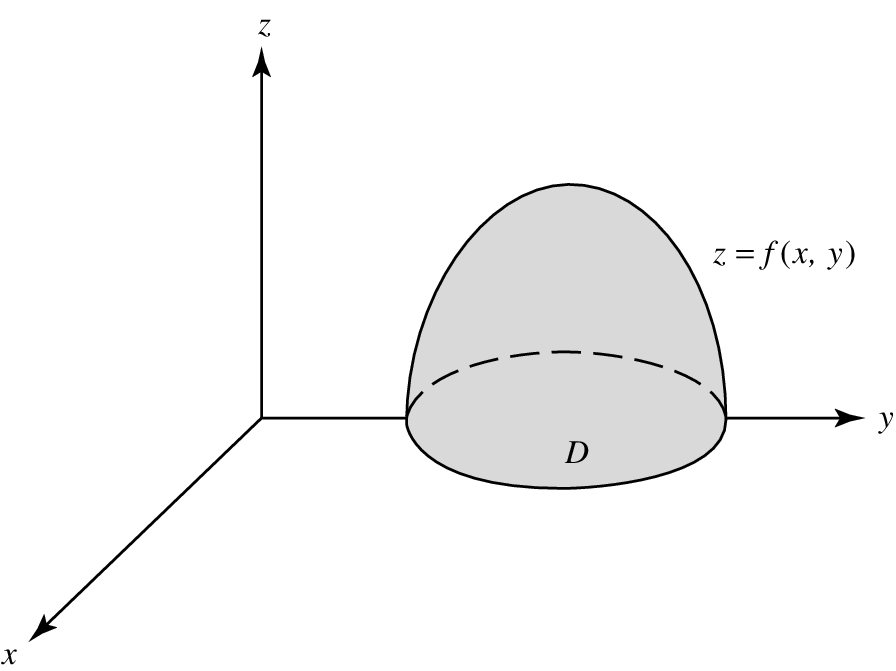
\includegraphics[width=3.1in,height=2.3in]{png/fig050301.png}
\end{center}
 \vskip6pt
 \refstepcounter{figure}
 \centerline{\bf Figure \thefigure} \label{figure:5.3.1}
 \vskip12pt
Differentiability
of
a function of $n$ variables has an analogous geometric interpretation.
We will illustrate it for $n=2$.
If $f$ is defined in a region $D$ in $\R^2$, then the set of
points
$(x,y,z)$ such that
\begin{equation}\label{eq:5.3.27}
z=f(x,y),\quad (x,y)\in D,
\end{equation}
is a {\it surface\/} in $\R^3$
(Figure~\ref{figure:5.3.1}).


 \vspace*{12pt}
\begin{center}
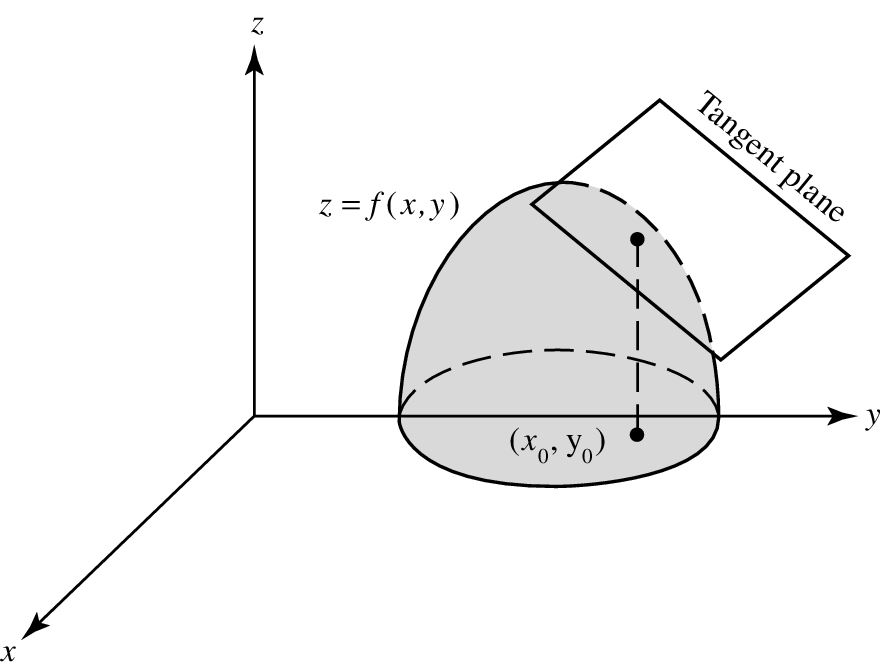
\includegraphics[width=3in,height=2.2in]{png/fig050302.png}
\end{center}
 \vskip6pt
 \refstepcounter{figure}
 \centerline{\bf Figure \thefigure} \label{figure:5.3.2}
 \vskip12pt

If
$f$ is differentiable at $\mathbf{X}_0=(x_0,y_0)$, then the plane
\begin{equation}\label{eq:5.3.28}
z=T(x,y)=f(\mathbf{X}_0)+f_x(\mathbf{X}_0)(x-x_0)+f_y(\mathbf{X}_0)(y-y_0)
\end{equation}
intersects the surface \eqref{eq:5.3.27} at
$(x_0,y_0,f(x_0,y_0))$ and approximates the surface so well
near $(x_0,y_0)$ that
\newpage

$$
\lim_{(x,y)\to (x_0,y_0)}\frac{f(x,y)-T(x,y)}{\sqrt{(x-x_0)^2+
(y-y_0)^2}}=0
$$
(Figure~\ref{figure:5.3.2}). Moreover,
\eqref{eq:5.3.28} is the only plane in
$\R^3$ with these properties (Exercise~\ref{exer:5.3.25}).
We
say that this plane is {\it tangent to the surface $z=f(x,y)$ at the
point} $(x_0,y_0,f(x_0,y_0))$. We will now show
that
it is the ``limit'' of ``secant planes'' associated with the surface
$z=f(x,y)$, just as a tangent line to a curve $y=f(x)$ in $\R^3$
is the limit of secant lines to the curve (Section~2.3).





Let $\mathbf{X}_i=(x_i,y_i)$ $(i=1,2,3)$. The equation of the ``secant
plane''
 through the points $(x_i,y_i,f(x_i,y_i))$ $(i=1,2,3)$ on
the surface $z=f(x,y)$ (Figure~\ref{figure:5.3.3})
 is of the form
\begin{equation}\label{eq:5.3.29}
z=f(\mathbf{X}_0)+A(x-x_0)+B(y-y_0),
\end{equation}
where $A$ and $B$ satisfy the system
\begin{eqnarray*}
f(\mathbf{X}_1)\ar=f(\mathbf{X}_0)+A(x_1-x_0)+B(y_1-y_0),\\
f(\mathbf{X}_2)\ar=f(\mathbf{X}_0)+A(x_2-x_0)+B(y_2-y_0).
\end{eqnarray*}
Solving for $A$ and $B$ yields
\begin{eqnarray}
A\ar=\frac{(f(\mathbf{X}_1)-f(\mathbf{X}_0))(y_2-y_0)-
(f(\mathbf{X}_2)-f(\mathbf{X}_0))
(y_1-y_0)}{(x_1-x_0)(y_2-y_0)-(x_2-x_0)(y_1-y_0)}\label{eq:5.3.30}\\
\arraytext{and}\nonumber\\
B\ar=\frac{(f(\mathbf{X}_2)-f(\mathbf{X}_0))(x_1-x_0)-
(f(\mathbf{X}_1)-f(\mathbf{X}_0))(x_2-x_0)}{(x_1-x_0)(y_2-y_0)-
(x_2-x_0)(y_1-y_0)}\label{eq:5.3.31}
\end{eqnarray}
if
\begin{equation}\label{eq:5.3.32}
(x_1-x_0)(y_2-y_0)-(x_2-x_0)(y_1-y_0)\ne0,
\end{equation}
which is equivalent to the requirement that $\mathbf{X}_0$, $\mathbf{X}_1$,
and $\mathbf{X}_2$ do not lie on a line (Exercise~\ref{exer:5.3.23}). If we
write
$$
\mathbf{X}_1=\mathbf{X}_0+t\mathbf{U}\mbox{\quad and\quad}\mathbf{X}_2=
\mathbf{X}_0+t\mathbf{V},
$$
where $\mathbf{U}=(u_1,u_2)$ and $\mathbf{V}=(v_1,v_2)$ are fixed nonzero
vectors (Figure~\ref{figure:5.3.3}), then \eqref{eq:5.3.30}, \eqref{eq:5.3.31},
and \eqref{eq:5.3.32} take the more convenient forms
\begin{eqnarray}
A\ar=\frac{\dst{\frac{f(\mathbf{X}_0+t\mathbf{U})-f(\mathbf{X}_0)}{ t} v_2-
\frac{ f(\mathbf{X}_0+t\mathbf{V})-f(\mathbf{X}_0)}{ t}u_2}}
{u_1v_2-u_2v_1},
\label{eq:5.3.33}\\
B\ar=\frac{\dst{\frac{f(\mathbf{X}_0+t\mathbf{V})-f(\mathbf{X}_0)}{ t} u_1-
\frac{ f(\mathbf{X}_0+t\mathbf{U})-f(\mathbf{X}_0)}{ t}v_1}}
{u_1v_2-u_2v_1},
\label{eq:5.3.34}
\end{eqnarray}
and
$$
u_1v_2-u_2v_1\ne0.
$$

\topfig{-3}
\begin{center}
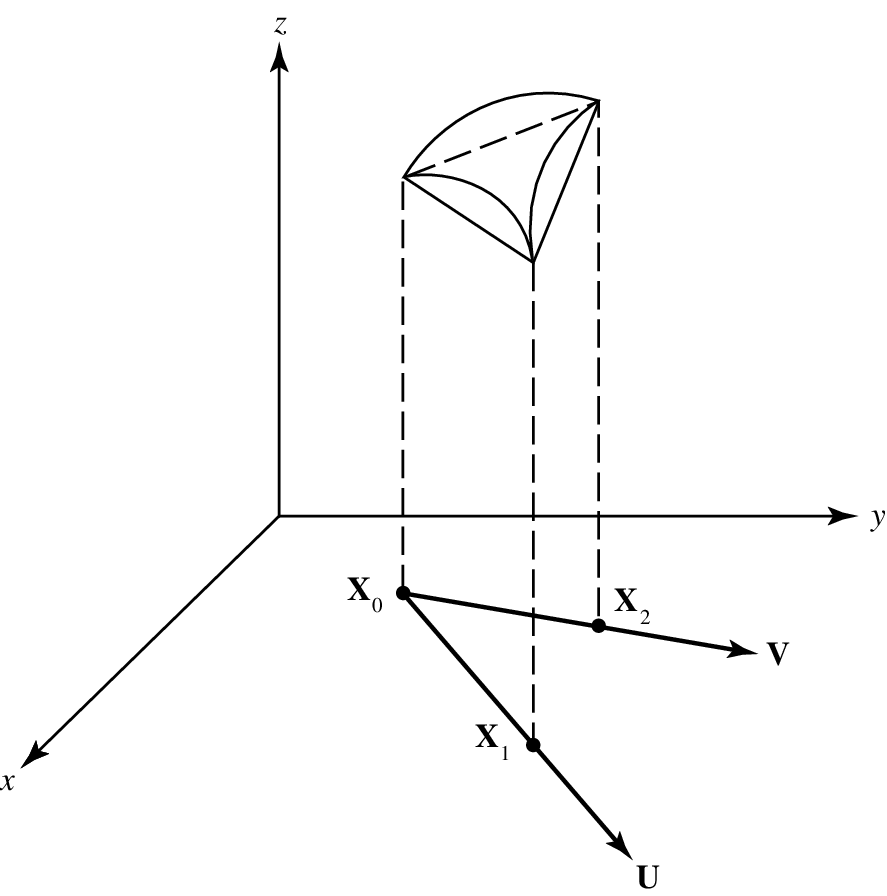
\includegraphics[width=3in,height=3in]{png/fig050303.png}
\end{center}
 \vskip6pt
 \refstepcounter{figure}
 \centerline{\bf Figure \thefigure} \label{figure:5.3.3}
 \vskip12pt

If $f$ is differentiable at $\mathbf{X}_0$, then
\begin{equation}\label{eq:5.3.35}
f(\mathbf{X})-f(\mathbf{X}_0)=f_x(\mathbf{X}_0) (x-x_0)+f_y(\mathbf{X}_0)(y-y_0)+
\epsilon(\mathbf{X}) |\mathbf{X}-\mathbf{X}_0|,
\end{equation}
where
\begin{equation}\label{eq:5.3.36}
\lim_{\mathbf{X}\to\mathbf{X}_0}\epsilon(\mathbf{X})=0.
\end{equation}
Substituting first $\mathbf{X}=\mathbf{X}_0+t\mathbf{U}$ and then $\mathbf{X}
=\mathbf{X}_0+t\mathbf{V}$ in \eqref{eq:5.3.35} and dividing by $t$ yields
\begin{equation}\label{eq:5.3.37}
\frac{f(\mathbf{X}_0+t\mathbf{U})-f(\mathbf{X}_0)}{ t}=f_x (\mathbf{X}_0)u_1+
f_y(\mathbf{X}_0)u_2+E_1(t) |\mathbf{U}|
\end{equation}
and
\begin{equation}\label{eq:5.3.38}
\frac{f(\mathbf{X}_0+t\mathbf{V})-f(\mathbf{X}_0)}{ t}=f_x (\mathbf{X}_0)v_1+
f_y(\mathbf{X}_0)v_2+E_2(t) |\mathbf{V}|,
\end{equation}
where
$$
E_1(t)=\epsilon(\mathbf{X}_0+t\mathbf{U})|t|/t\mbox{\quad and\quad} E_2(t)=
\epsilon(\mathbf{X}_0+t\mathbf{V})|t|/t,
$$
so
\begin{equation}\label{eq:5.3.39}
\lim_{t\to 0} E_i(t)=0,\quad i=1,2,
\end{equation}
 because of \eqref{eq:5.3.36}.
Substituting \eqref{eq:5.3.37} and \eqref{eq:5.3.38} into \eqref{eq:5.3.33} and
\eqref{eq:5.3.34} yields
\begin{equation}\label{eq:5.3.40}
A=f_x(\mathbf{X}_0)+\Delta_1(t),\quad B=f_y(\mathbf{X}_0)+\Delta_2(t),
\end{equation}
\nopagebreak
where
\newpage
\vspace*{-2pc}
$$
\Delta_1(t)=\frac{v_2 |\mathbf{U}|E_1(t)-u_2|\mathbf{V}|E_2(t)}{
u_1v_2-u_2v_1}
$$
and
$$
\Delta_2(t)=\frac{u_1|\mathbf{V}|E_2(t)-v_1|\mathbf{U}|E_1(t)}{
u_1v_2-u_2v_1},
$$
so
\begin{equation}\label{eq:5.3.41}
\lim_{t\to 0}\Delta_i(t)=0,\quad i=1,2,
\end{equation}
 because of \eqref{eq:5.3.39}.

From \eqref{eq:5.3.29} and \eqref{eq:5.3.40}, the equation of the secant plane
is
$$
z=f(\mathbf{X}_0)+[f_x(\mathbf{X}_0)+\Delta_1(t)](x-x_0)+
[f_y(\mathbf{X}_0)+\Delta_2(t)](y-y_0).
$$
Therefore, because of \eqref{eq:5.3.41}, the secant plane ``approaches''
the tangent plane \eqref{eq:5.3.28} as $t$ approaches zero.

\boxit{Maxima and Minima}
We say that $\mathbf{X}_0$ is a {\it local extreme point\/} of $f$ if there
is a $\delta>0$ such that
$$
f(\mathbf{X})-f(\mathbf{X}_0)
$$
does not change sign in $S_\delta (\mathbf{X}_0)\cap D_f$. More
specifically, $\mathbf{X}_0$ is a {\it local maximum point\/} if
$$
f(\mathbf{X})\le f(\mathbf{X}_0)
$$
or a {\it local minimum point\/} if
$$
f(\mathbf{X})\ge f(\mathbf{X}_0)
$$
for all $\mathbf{X}$ in $S_\delta (\mathbf{X}_0)\cap D_f$.

The next theorem is analogous to Theorem~\ref{thmtype:2.3.7}.

\begin{theorem}\label{thmtype:5.3.11}
Suppose that  $f$ is defined in a neighborhood of $\mathbf{X}_0$ in
$\R^n$  and $f_{x_1}(\mathbf{X}_0),$ $f_{x_2}(\mathbf{X}_{0}),$
 \dots$,$ $f_{x_n}(\mathbf{X}_{0})$
 exist$.$ Let $\mathbf{X}_0$ be a local extreme point of $f.$ Then
\begin{equation}\label{eq:5.3.42}
f_{x_i}(\mathbf{X}_0)=0,\quad 1\le i\le n.
\end{equation}
\end{theorem}

\proof  Let
$$
\mathbf{E}_1=(1,0, \dots,0),\quad \mathbf{E}_{2}
=(0,1,0, \dots,0),\dots,\quad \mathbf{E}_n=
(0,0, \dots,1),
$$
and
$$
g_i(t)=f(\mathbf{X}_0+t\mathbf{E}_i),\quad 1\le i\le n.
$$
Then $g_i$ is differentiable at $t=0$, with
$$
g'_i(0)=f_{x_i}(\mathbf{X}_0)
$$
\newpage
\noindent
(Definition~\ref{thmtype:5.3.1}). Since $\mathbf{X}_0$ is a local extreme
point of $f$, $t_0=0$ is a local extreme point of $g_i$. Now
Theorem~\ref{thmtype:2.3.7} implies that $g'_i(0)=0$, and this
implies \eqref{eq:5.3.42}.
\bbox

The converse of Theorem~\ref{thmtype:5.3.11} is false, since \eqref{eq:5.3.42}
may hold at a point $\mathbf{X}_0$ that is not a local extreme point of
$f$. For example, let $\mathbf{X}_0= (0,0)$ and
$$
f(x,y)=x^3+y^3.
$$
We  say that a point $\mathbf{X}_0$ where \eqref{eq:5.3.42} holds is a
{\it critical point\/} of
$f$. Thus, if
$f$ is defined in a neighborhood
of a local extreme point $\mathbf{X}_0$, then $\mathbf{X}_0$ is a critical
point of $f$; however, a critical point need not be a local extreme
point of $f$.

The use of Theorem~\ref{thmtype:5.3.11} for finding local extreme points
is covered in  calculus, so we will not pursue
it here.

\exercises
\begin{exerciselist}



\item\label{exer:5.3.1} Calculate $\partial
f(\mathbf{X})/\partial\boldsymbol{\Phi}$.
\begin{alist}
\item % (a)
 $f(x,y)=x^2+2xy\cos x$,\quad $\dst\boldsymbol{\Phi}=
\left(\frac{1}{\sqrt3},-\sqrt{\frac{2}{3}}\right)$
\item % (b)
 $f(x,y,z)=e^{-x+y^2+2z}$,\quad $\dst{\boldsymbol{\Phi}=
\left(\frac{1}{\sqrt{3}},-\frac{1}{\sqrt{3}},
\frac{1}{\sqrt{3}}\right)}$
\item % (c)
 $f(\mathbf{X})=|\mathbf{X}|^2$,\quad $\dst{\boldsymbol{\Phi}=
\left(\frac{1}{\sqrt{n}},\quad\frac{1}{\sqrt{n}},\cdots,\frac{1}{\sqrt{n}}
\right)}$
\item % (d)
 $f(x,y,z)=\log(1+x+y+z)$,\quad $\boldsymbol{\Phi}=(0,1,0)$
\end{alist}

\item\label{exer:5.3.2} Let
$$
f(x,y)=\left\{\casespace\begin{array}{ll}\dst
\frac{xy\sin x}{ x^2+y^2},&(x,y)\ne
(0,0),\\[2\jot]
 0,&(x,y)=(0,0),
\end{array}\right.
$$
and let $\boldsymbol{\Phi}=(\phi_1,\phi_2)$ be a unit vector. Find $\partial
f(0,0)/\partial\boldsymbol{\Phi}$.

\item\label{exer:5.3.3}
 Find $\partial f(\mathbf{X}_0)/\partial\boldsymbol{\Phi}$,
where $\boldsymbol{\Phi}$ is the unit vector in the direction of
$\mathbf{X}_1-\mathbf{X}_{)}$.
\begin{alist}
\item % (a)
 $f(x,y,z)=\sin\pi xyz$;\quad $\mathbf{X}_0=(1,1,-2)$,\quad
$\mathbf{X}_1=(3,2,-1)$
\item % (b)
 $f(x,y,z)=e^{-(x^2+y^2+2z)}$;\quad $\mathbf{X}_0=(1,0,-1)$,
\quad$\mathbf{X}_1=(2,0,-1)$
\item % (c)
$f(x,y,z)=\log(1+x+y+z)$;\quad $\mathbf{X}_0=(1,0,1)$,\quad
$\mathbf{X}_1=(3,0,-1)$
\item % (d)
$f(\mathbf{X})=|\mathbf{X}|^4$;\quad $\mathbf{X}_0=\mathbf{0}$,\quad
$\mathbf{X}_1=(1,1, \dots,1)$
\end{alist}

\item\label{exer:5.3.4} Give a geometrical interpretation of the
directional derivative  $\partial f(x_0,y_0)/\partial\boldsymbol{\Phi}$ of a
function of two variables.

\item\label{exer:5.3.5} Find all first-order partial derivatives.

\hskip-.5em
\begin{tabular}{ll}
\part{a} $f(x,y,z)=\log(x+y+2z)$&
\part{b}  $f(x,y,z)=x^2+3xyz+2xy$\\[2\jot]
\part{c} $f(x,y,z)=xe^{yz}$ &
\part{d} $f(x,y,z)=z+\sin x^2y$
\end{tabular}

\nopagebreak
\item\label{exer:5.3.6} Find all second-order partial derivatives of the
functions in Exercise~\ref{exer:5.3.5}.
\newpage

\item\label{exer:5.3.7}
 Find all second-order partial derivatives of the following functions
at
$(0,0)$.
\begin{alist}
\item % (a)
 $\dst{f(x,y)=\left\{\casespace\begin{array}{ll}
\dst\frac{xy(x^2-y^2}{ x^2+y^2},&(x,y)\ne (0,0),\\[2\jot]
 0,&(x,y)=(0,0)
\end{array}\right.}$
\item % (b)
 $\dst{f(x,y)=\left\{\casespace\begin{array}{ll}\dst{x^2\tan^{-1}
\frac{y}{ x}-y^2\tan^{-1}\frac{x}{ y}},&x\ne0,\quad y\ne0,\\[2\jot]
 0,&x=0\mbox{\quad or\quad} y=0\end{array}\right.}$
\end{alist}
(Here $|\tan^{-1}u|<\pi/2$.)

\item\label{exer:5.3.8} Find a function $f=f(x,y)$  such
that
$f_{xy}$ exists for all $(x,y)$, but $f_y$ exists nowhere.

\item\label{exer:5.3.9} Let $u$ and $v$ be functions of two variables
with continuous  second-order partial derivatives in a region $S$.
Suppose that
$u_x=v_y$ and $u_y=-v_x$
in $S$.  Show that
$$
u_{xx}+u_{yy}=v_{xx}+v_{yy}=0
$$
in $S$.

\item\label{exer:5.3.10} Let $f$ be a function of
$(x_1,x_2, \dots,x_n)$ $(n\ge2)$ such that $f_{x_i}$, $f_{x_j}$, and
$f_{x_ix_j}$ $(i\ne j)$ exist on a neighborhood of $\mathbf{X}_0$ and
$f_{x_ix_j}$ is continuous at $\mathbf{X}_0$. Use Theorem~\ref{thmtype:5.3.3}
to prove that $f_{x_jx_i}(\mathbf{X}_0)$ exists and equals
$f_{x_ix_j}(\mathbf{X}_0)$.

\item\label{exer:5.3.11} Use Exercise~\ref{exer:5.3.10} and
induction on $r$ to prove Theorem~\ref{thmtype:5.3.4}.

\item\label{exer:5.3.12}
 Let $r_1,r_2, \dots,r_n$ be nonnegative integers
such that
$$
r_1+r_2+\cdots+r_n=r\ge0.
$$
\begin{alist}
\item % (a)
 Show that
$$
(z_1+z_2+\cdots+z_n)^r=\sum_r\frac{r!}{ r_1!r_2!\cdots
r_n!}z^{r_1}_1z^{r_2}_2\cdots z^{r_n}_n,
$$
where $\sum_r$ denotes summation over all $n$-tuples $(r_1,r_2, \dots,r_n)$
that satisfy the stated conditions. \hint{This is obvious if
 $n=1,$ and it  follows
from Exercise~$\ref{exer:1.2.19}$ if $n=2.$  Use induction on
$n.$}
\item % (b)
 Show that there are
$$
\frac{r!}{ r_1!r_2!\cdots r_n!}
$$
ordered $n$-tuples of integers $(i_1,i_2, \dots,i_n)$ that contain
$r_1$
 ones, $r_2$ twos, \dots, and $r_n$
$n$'s.
\item % (c)
 Let $f$ be a function of $(x_1,x_2, \dots,x_n)$.  Show that
there are
$$
\frac{r!}{ r_1!r_2!\cdots r_n!}
$$
partial derivatives $f_{x_{i_1}x_{i_2}\cdots x_{i_r}}$ that involve
differentiation $r_i$ times with respect to $x_i$, for $i=1,2, \dots,n$.
\end{alist}

\nopagebreak

\item\label{exer:5.3.13} Prove Lemma~\ref{thmtype:5.3.8}.

\newpage

\item\label{exer:5.3.14}
Show that the function
$$
f(x,y)=\left\{\casespace\begin{array}{ll}
\dst\frac{x^2y}{ x^6+2y^2},&(x,y)\ne
(0,0),\\[2\jot]
 0,&(x,y)=(0,0),\end{array}\right.
$$
has a directional derivative in the direction of an arbitrary unit
vector $\Phi$ at
$(0,0)$, but $f$ is not continuous at $(0,0)$.

\item\label{exer:5.3.15} Prove: If $f_x$ and $f_y$ are bounded in a
neighborhood of $(x_0,y_0)$, then $f$ is continuous at $(x_0,y_0)$.

\item\label{exer:5.3.16} Show directly from
Definition~\ref{thmtype:5.3.5} that $f$ is differentiable at $\mathbf{X}_0$.
\begin{alist}
\item % (a)
 $f(x,y)=2x^2+3xy+y^2$,\quad $\mathbf{X}_0=(1,2)$
\item % (b)
 $f(x,y,z)=2x^2+3x+4yz$,\quad $\mathbf{X}_0=(1,1,1)$
\item % (c)
 $f(\mathbf{X})=|\mathbf{X}|^2$,\quad $\mathbf{X}_0$ arbitrary
\end{alist}


\item\label{exer:5.3.17}
 Suppose that  $f_x$ exists on a neighborhood of $(x_0,y_0)$ and is
continuous at $(x_0,y_0)$, while $f_y$ merely exists at $(x_0,y_0)$.  Show
that $f$ is differentiable at $(x_0,y_0)$.

\item\label{exer:5.3.18}
Find $df$ and $d_{\mathbf{X}_0}f$, and write
$(d_{\mathbf{X}_0}f)(\mathbf{X}-\mathbf{X}_0)$.
\begin{alist}
\item % (a)
 $f(x,y)=x^3+4xy^2+2xy\sin x$,\quad $\mathbf{X}_0=(0,-2)$
\item % (b)
 $f(x,y,z)=e^{-(x+y+z)}$,\quad $\mathbf{X}_0=(0,0,0)$
\item % (c)
 $f(\mathbf{X})=\log(1+x_1+2x_2+3x_3+\cdots+nx_n)$,\quad
$\mathbf{X}_0=\mathbf{0}$
\item % (d)
 $f(\mathbf{X})=|\mathbf{X}|^{2r}$,\quad $\mathbf{X}_0=
(1,1,1, \dots,1)$
\end{alist}

\item\label{exer:5.3.19}
\begin{alist}
\item % (a)
 Suppose that  $f$ is differentiable at $\mathbf{X}_0$ and $\boldsymbol{\Phi}
=(\phi_1,\phi_2, \dots,\phi_n)$ is a unit vector.  Show that
$$
\frac{\partial
f(\mathbf{X}_0)}{\partial\boldsymbol{\Phi}}=f_{x_1}(\mathbf{X}_{0})
\phi_1+f_{x_2}(\mathbf{X}_0)\phi_2+\cdots+f_{x_n}(\mathbf{X}_0)\phi_n.
$$
\item % (b)
 For what unit vector $\boldsymbol{\Phi}$ does $\partial f(\mathbf{X}_{0})
/\partial\boldsymbol{\Phi}$ attain its maximum value?
\end{alist}


\item\label{exer:5.3.20}
Let $f$  be defined on $\R^n$  by
$$
f(\mathbf{X})=g(x_1)+g(x_2)+\cdots+g(x_n),
$$
where
$$
g(u)=
\left\{\casespace\begin{array}{ll}
u^2\sin\dst\frac{1}{u},&u\ne0,\\
0,&u=0.
\end{array}\right.
$$
Show that $f$ is differentiable at $(0,0, \dots,0)$, but $f_{x_1}$,
$f_{x_2}$, \dots,
$f_{x_n}$ are all discontinuous  at $(0,0, \dots,0)$.



\item\label{exer:5.3.21}
The purpose of this exercise is to show that if $f$, $f_x$
and $f_y$  exist on a neighborhood $N$ of $(x_0,y_0)$ and
$f_x$  and $f_y$ are differentiable at $(x_0,y_0)$, then
$f_{xy}(x_0,y_0)=f_{yx}(x_0,y_0)$.
Suppose that
the open square
$$
\set{(x,y)}{|x-x_0|<|h|, |y-y_0|<|h|}
$$
\newpage
\noindent
is in $N$. Consider
$$
B(h)=f(x_0+h, y_0+h)-f(x_0+h,y_0)-f(x_0,y_0+h)+f(x_0,y_0).
$$
\begin{alist}
\item % (a)
Use the mean value theorem as we did in the proof of
Theorem~\ref{thmtype:5.3.3} to write
$$
B(h)=\left[f_x (\widehat{x},y_0+k)-f_x(\widehat{x},y_0)\right]h,
$$
where $\widehat{x}$ is between $x_0$ and $x_0+h$. Then use the
differentiability of $f_x$ at $(x_0,y_0)$ to infer that
$$
B(h)=h^2f_{xy}(x_0,y_0)+hE_1(h),
\mbox{\quad where \quad} \lim_{h\to0}\frac{E_1(h)}{h}=0.
$$
\item % (b)
Use the mean value theorem  to write
$$
B(h)=\left[f_y (x_0+h,\widehat y)-f_y(x_0,\widehat y)\right]h,
$$
where $\widehat{y}$ is between $y_0$ and $y_0+h$. Then use the
differentiability of $f_y$ at $(x_0,y_0)$ to infer that
$$
B(h)=h^2f_{yx}(x_0,y_0)+hE_2(h),
\mbox{\quad where \quad} \lim_{h\to0}\frac{E_2(h)}{h}=0.
$$
\item % (c)
Infer from \part{a} and \part{b} that
$f_{xy}(x_0,y_0)=f_{yx}(x_0,y_0)$.
\end{alist}

\item\label{exer:5.3.22}
\begin{alist}
\item % (a)
Let $f_{x_i}$ and $f_{x_j}$ be differentiable at a point $\mathbf{X}_0$
in $\R^n$. Show from Exercise~\ref{exer:5.3.21} that
$$
f_{x_ix_j}(\mathbf{X}_0)=f_{x_jx_i}(\mathbf{X}_0).
$$
\item % (b)
Use \part{a}  and
induction on $r$  to show that
 all $(r-1)$-st order partial
derivatives of $f$ are differentiable on an open subset $S$ of
$\R^n$, then
$f_{x_{i_1}x_{i_2}\cdots x_{i_r}}(\mathbf{X})$ ($\mathbf{X}\in S$) depends
only on the number of
differentiations with respect to each variable, and not on the order
in which they are performed.
\end{alist}

\item\label{exer:5.3.23}
Prove that $(x_0,y_0)$, $(x_1,y_1)$, and $(x_2,y_2)$ lie on a line if
and only if
$$
(x_1-x_0)(y_2-y_0)-(x_2-x_0)(y_1-y_0)=0.
$$

\item\label{exer:5.3.24}
Find the equation of the tangent plane to the surface
$$
z=f(x,y)\mbox{\quad at \quad}(x_0,y_0,z_0)=(x_0,y_0,f(x_0,y_0)).
$$
\begin{alist}
\item % (a)
$f(x,y)=x^2+y^2-1,\quad (x_0,y_0)=(1,2)$
\item % (b)
$f(x,y)=2x+3y+1,\quad (x_0,y_0)=(1,-1)$
\item % (c)
$f(x,y)=xy\sin xy,\quad (x_0,y_0)=(1,\pi/2)$
\item % (d)
$f(x,y)=x^2-2y^2+3xy,\quad (x_0,y_0)=(2,-1)$
\end{alist}

\item\label{exer:5.3.25}
Prove: If $f$ is differentiable at $(x_0,y_0)$ and
$$
\lim_{(x,y)\to(x_0,y_0)}\frac{f(x,y)-a-b(x-x_0)-c(y-y_0)
}{\sqrt{(x-x_0)^2+(y-y_0)^2}}=0,
$$
then $a=f(x_0,y_0)$, $b=f_x(x_0,y_0)$, and $c=f_y(x_0,y_0)$.


\label{sectionend:\thesection} \end{exerciselist}


\currentpdfbookmark{Section 5.4 The Chain Rule and Taylor's
Theorem}{section:5.4}
\newsection{4}
{Real-Valued Functions of Several Variables}
{The Chain Rule and Taylor's Theorem}


\renewcommand{\thissection}{\sectiontitle {THE CHAIN RULE AND TAYLOR'S
THEOREM}} \thissection

\noindent
We now consider the problem of differentiating a composite function
$$
h(\mathbf{U})=f(\mathbf{G}(\mathbf{U})),
$$
 where $\mathbf{G}=(g_1,g_2, \dots,g_n)$
is a vector-valued function, as defined in Section~5.2.
We begin with the following definition.


\begin{definition} \label{thmtype:5.4.1} \rm
A vector-valued function
 $\mathbf{G}=(g_1,g_2, \dots,g_n)$ is {\it
differentiable\/} at
$$
\mathbf{U}_0=(u_{10},u_{20}, \dots,u_{m0})
$$
 if its component functions
$g_1$, $g_2$, \dots, $g_n$ are differentiable at $\mathbf{U}_0$.
\bbox\end{definition}

We need the following lemma to prove the main result of the section.

\begin{lemma} \label{thmtype:5.4.2}
Suppose that  $\mathbf{G}=(g_1,g_2, \dots,g_n)$ is differentiable at
$$
 \mathbf{U}_0=(u_{10}, u_{20}, \dots,u_{m0}),
$$
 and
 define
$$
M=\left(\sum_{i=1}^n\sum_{j=1}^m\left(\frac{\partial g_i(\mathbf{U}_0}
{\partial u_j}\right)^2\right)^{1/2}.
$$
Then$,$ if $\epsilon>0,$ there is a $\delta>0$ such that
$$
\frac{|\mathbf{G}(\mathbf{U})-\mathbf{G}(\mathbf{U}_0)|}
{|\mathbf{U}-\mathbf{U}_{0}|}
<M+\epsilon\mbox{\quad if \quad}0<|\mathbf{U}-\mathbf{U}_0|<\delta.
$$
\end{lemma}

\proof
Since $g_1$, $g_2$, \dots, $g_n$ are differentiable at $\mathbf{U}_0$,
applying
Lemma~\ref{thmtype:5.3.8} to $g_i$ shows that
\begin{equation} \label{eq:5.4.1}
\begin{array}{rcl}
g_i(\mathbf{U})-g_i(\mathbf{U}_0)\ar=(d_{\mathbf{U}_0}g_i)(\mathbf{U}-\mathbf{U}_0)+
E_i (\mathbf{U}) |(\mathbf{U}-\mathbf{U}_0|\\[2\jot]
\ar=\dst\sum_{j=1}^m\frac{\partial g_i(\mathbf{U}_0)}{\partial
u_j}(u_j-u_{j0})+
E_i (\mathbf{U}) |(\mathbf{U}-\mathbf{U}_0|,
\end{array}
\end{equation}
\newpage
\noindent
where
\begin{equation} \label{eq:5.4.2}
\lim_{\mathbf{U}\to\mathbf{U}_0}E_i(\mathbf{U})=0,\quad 1\le i\le n.
\end{equation}
From Schwarz's inequality,
$$
|g_i(\mathbf{U})-g_i(\mathbf{U}_0)|\le(M_i+|E_i(\mathbf{U})|)
|\mathbf{U}-\mathbf{U}_{0}|,
$$
where
$$
M_i=\left(\sum_{j=1}^m\left(\frac{\partial g_i(\mathbf{U}_0)}
{\partial u_j}\right)^2\right)^{1/2}.
$$
Therefore,
$$
\frac{|\mathbf{G}(\mathbf{U})-\mathbf{G}(\mathbf{U}_0)|}{|\mathbf{U}-\mathbf{U}_0|}
\le\left(\sum_{i=1}^n(M_i+|E_i(\mathbf{U})|)^2\right)^{1/2}.
$$
From \eqref{eq:5.4.2},
$$
\lim_{\mathbf{U}\to\mathbf{U}_0}
\left(\sum_{i=1}^n(M_i+|E_i(\mathbf{U})|)^2\right)^{1/2}
=\left(\sum_{i=1}^nM_i^2\right)^{1/2}=M,
$$
which implies the conclusion.
\bbox

The following theorem is analogous to
Theorem~\ref{thmtype:2.3.5}.


\begin{theorem} [The Chain Rule] \label{thmtype:5.4.3}
Suppose that  the real-valued function $f$ is differentiable at
$\mathbf{X}_0$
in $\R^n,$ the vector-valued function $\mathbf{G}
=(g_1,g_2, \dots,g_n)$ is differentiable at
$\mathbf{U}_0$ in $\R^m,$ and $\mathbf{X}_{0}
 = \mathbf{G}(\mathbf{U}_0).$ Then the real-valued composite function
$h=f\circ\mathbf{G}$ defined by
\begin{equation} \label{eq:5.4.3}
h(\mathbf{U})=f(\mathbf{G}(\mathbf{U}))
\end{equation}
is differentiable at $\mathbf{U}_0,$ and
\begin{equation} \label{eq:5.4.4}
d_{\mathbf{U}_0}h=f_{x_1}(\mathbf{X}_0) d_{\mathbf{U}_0}g_1+f_{x_2}
(\mathbf{X}_0) d_{\mathbf{U}_0}g_2+\cdots
+f_{x_n} (\mathbf{X}_0) d_{\mathbf{U}_0}g_n.
\end{equation}
\end{theorem}


\proof
We leave it to you to show that $\mathbf{U}_0$ is an interior point
of the domain of $h$ (Exercise~\ref{exer:5.4.1}), so it is legitimate to
ask if $h$ is differentiable at $\mathbf{U}_0$.

Let $\mathbf{X}_0=(x_{10},x_{20}, \dots,x_{n0})$. Note that
$$
x_{i0}=g_i(\mathbf{U}_0),\quad
1\le i\le n,
$$
by assumption.
Since $f$ is differentiable at $\mathbf{X}_0$,
Lemma~\ref{thmtype:5.3.8} implies that
\begin{equation} \label{eq:5.4.5}
f(\mathbf{X})-f(\mathbf{X}_0)=\sum_{i=1}^n f_{x_i} (\mathbf{X}_0)
(x_i-x_{i0})+E(\mathbf{X})|\mathbf{X}-\mathbf{X}_0|,
\end{equation}
where
$$
\lim_{\mathbf{X}\to\mathbf{X}_0}E(\mathbf{X})=0.
$$
\newpage
\noindent
 Substituting $\mathbf{X}=\mathbf{G}(\mathbf{U})$
 and $\mathbf{X}_0=\mathbf{G}(\mathbf{U}_0)$ in \eqref{eq:5.4.5} and recalling
\eqref{eq:5.4.3} yields
\begin{equation} \label{eq:5.4.6}
h(\mathbf{U})-h(\mathbf{U}_0)=\dst{\sum_{i=1}^n}\, f_{x_i}(\mathbf{X}_0)
(g_i(\mathbf{U})-g_i(\mathbf{U}_0))
+E(\mathbf{G}(\mathbf{U}))
|\mathbf{G}(\mathbf{U})-\mathbf{G}(\mathbf{U}_0)|.
\end{equation}
Substituting \eqref{eq:5.4.1} into \eqref{eq:5.4.6} yields
$$
\begin{array}{rcl}
h(\mathbf{U})-h(\mathbf{U}_0)\ar=\dst{\sum_{i=1}^n} f_{x_i}(\mathbf{X}_0)
(d_{\mathbf{U}_0}g_i) (\mathbf{U}-\mathbf{U}_0)
+\dst{\left(\sum_{i=1}^n
f_{x_i}(\mathbf{X}_0)E_i(\mathbf{U})\right)} |\mathbf{U}-\mathbf{U}_0|
\\\\
\ar{}+E(\mathbf{G}(\mathbf{U}))
|\mathbf{G}(\mathbf{U})-\mathbf{G}(\mathbf{U}_{0}|.
\end{array}
$$
Since
$$
\lim_{\mathbf{U}\to\mathbf{U}_0}E(\mathbf{G}(\mathbf{U}))=\lim_{\mathbf{X}\to\mathbf{X}_0}E(\mathbf{X})=0,
$$
\eqref{eq:5.4.2} and Lemma~\ref{thmtype:5.4.2}  imply that
$$
\frac{h(\mathbf{U})-h(\mathbf{U}_0)-\dst\sum_{i=1}^nf_{x_i}(\mathbf{X}_{0}
d_{\mathbf{U}_0}g_i
(\mathbf{U}-\mathbf{U}_0)}{|\mathbf{U}-\mathbf{U}_0|}=0.
$$
Therefore, $h$ is differentiable at $\mathbf{U}_0$, and $d_{\mathbf{U}_0}h$
is given by \eqref{eq:5.4.4}.
\bbox


\begin{example}\label{example:5.4.1}\rm    Let
$$
f(x,y,z)=2x^2+4xy+3yz,
$$
$$
g_1(u,v)=u^2+v^2,\quad g_2(u,v)=u^2-2v^2,\quad g_3(u,v)=uv,
$$
and
$$
h(u,v)=f(g_1(u,v), g_2(u,v), g_3(u,v)).
$$
Let $\mathbf{U}_0=(1,-1)$ and
$$
\mathbf{X}_0=(g_1(\mathbf{U}_0), g_2(\mathbf{U}_0),
g_3(\mathbf{U}_0))=(2,-1,-1).
$$
Then
$$
f_x(\mathbf{X}_0)=4,\quad f_y(\mathbf{X}_0)=5,\quad f_z(\mathbf{X}_0)=-3,
$$
\begin{eqnarray*}
\frac{\partial g_1(\mathbf{U}_0)}{\partial
u}=\phantom{-}2,&\dst\frac{\partial g_1(\mathbf{U}_0)}{\partial
v}=-2,\\
\frac{\partial g_2(\mathbf{U}_0)}{\partial
u}=\phantom{-}2,&\dst\frac{\partial
g_2(\mathbf{U}_0)}{\partial v}=\phantom{-}4,\\
\frac{\partial g_3(\mathbf{U}_0)}{\partial u}=-1,&\dst\frac{\partial g_3
(\mathbf{U}_0)}{\partial v}=\phantom{-}1.
\end{eqnarray*}
Therefore,
$$
d_{\mathbf{U}_0}g_1=2\,du-2\,dv,\quad d_{\mathbf{U}_0}g_2=2\,du+4\,dv,\quad
d_{\mathbf{U}_0}g_3=-du+dv,
$$
\newpage
\noindent
and, from \eqref{eq:5.4.4},
\begin{eqnarray*}
d_{\mathbf{U}_0}h\ar=f_x(\mathbf{X}_0)\,d_{\mathbf{U}_0}g_1+
f_y(\mathbf{X}_0)\,d_{\mathbf{U}_0}g_2+
f_z(\mathbf{X}_0)\,d_{\mathbf{U}_0}g_3\\[2\jot]
\ar=4(2\,du-2\,dv)+5(2\,du+4\,dv)-3(-du+dv)\\[2\jot]
\ar=21\,du+9\,dv.
\end{eqnarray*}
Since
$$
d_{\mathbf{U}_0}h=h_u(\mathbf{U}_0)\,du+h_v(\mathbf{U}_0)\,dv
$$
we conclude that
\begin{equation} \label{eq:5.4.7}
h_u(\mathbf{U}_0)=21\mbox{\quad and\quad} h_v(\mathbf{U}_0)=9.
\end{equation}
This  can also be obtained by writing $h$ explicitly in terms of
$(u,v)$ and differentiating; thus,
\begin{eqnarray*}
h(u,v)\ar=2[g_1(u,v)]^2+4g_1(u,v) g_2(u,v)+3g_2(u,v)g_3(u,v)\\[2\jot]
\ar=2(u^2+v^2)^2+4(u^2+v^2)(u^2-2v^2)+3(u^2-2v^2)uv\\[2\jot]
\ar=6u^4+3u^3v-6uv^3-6v^4.
\end{eqnarray*}
Hence,
$$
h_u(u,v)=24u^3+9u^2v-6v^3\mbox{\quad and \quad}
h_v(u,v)=3u^3-18uv^2-24v^3,
$$
so  $h_u(1,-1)=21$ and $h_v(1,-1)=9$, consistent with \eqref{eq:5.4.7}.
\end{example}

\begin{corollary} \label{thmtype:5.4.4}
 Under the assumptions of Theorem~$\ref{thmtype:5.4.3},$
\begin{equation} \label{eq:5.4.8}
\frac{\partial h(\mathbf{U}_0)}{\partial u_i}=\sum_{j=1}^n \frac{\partial
f(\mathbf{X}_0)
}{\partial x_j} \frac{\partial g_j(\mathbf{U}_0)}{\partial u_i},\quad
1\le i
\le m.
\end{equation}
\end{corollary}

\proof
 Substituting
$$
d_{\mathbf{U}_0}g_i=\frac{\partial g_i(\mathbf{U}_0)}{\partial u_1}
\,du_1+\frac{\partial
g_i(\mathbf{U}_0)}{\partial u_2} \,du_2+\cdots+
\frac{\partial g_i(\mathbf{U}_0)}{
\partial u_m} \,du_m,\quad 1\le i\le n,
$$
into \eqref{eq:5.4.4} and collecting multipliers of
$du_1$, $du_2$, \dots, $du_m$ yields
$$
d_{\mathbf{U}_0}h=\sum_{i=1}^m\left(\sum_{j=1}^n
\frac{\partial f(\mathbf{X}_0)}{\partial
x_j} \frac{\partial g_j(\mathbf{U}_0)}{\partial u_i}\right)\,du_i.
$$
However, from Theorem~\ref{thmtype:5.3.6},
$$
d_{\mathbf{U}_0} h=\sum_{i=1}^m\frac{\partial h(\mathbf{U}_0)}{\partial u_i} \,du_i.
$$
\nopagebreak
Comparing the last two equations yields \eqref{eq:5.4.8}.
\bbox
\newpage

When it is not important to emphasize the particular point $\mathbf{X}_0$,
we write \eqref{eq:5.4.8} less formally as
\begin{equation} \label{eq:5.4.9}
\frac{\partial h}{\partial u_i}=\sum_{j=1}^n\frac{\partial f}{\partial
x_j} \frac{\partial g_j}{\partial u_i},\quad 1\le i\le m,
\end{equation}
with the understanding that in calculating
$\partial h(\mathbf{U}_0)/\partial
u_i$, $\partial g_j/\partial u_i$ is evaluated at $\mathbf{U}_0$ and
$\partial f/\partial x_j$ at $\mathbf{X}_0=\mathbf{G}(\mathbf{U}_0)$.

The formulas \eqref{eq:5.4.8} and \eqref{eq:5.4.9} can also be simplified by
replacing the symbol $\mathbf{G}$ with $\mathbf{X}=\mathbf{X}(\mathbf{U})$; then we
write
$$
h(\mathbf{U})=f(\mathbf{X}(\mathbf{U}))
$$
and
$$
\frac{\partial h(\mathbf{U}_0)}{\partial u_i}=\sum_{j=1}^n \frac{\partial
f(\mathbf{X}_0)}{ \partial x_j} \frac{\partial x_j(\mathbf{U}_0)}{\partial
u_i},
$$
or simply
\begin{equation} \label{eq:5.4.10}
\frac{\partial h}{\partial u_i}=\sum_{j=1}^n\frac{\partial f}{\partial
x_j} \frac{\partial x_j}{\partial u_i}.
\end{equation}

\begin{example}\label{example:5.4.2}\rm  Let $(r,\theta)$ be polar
coordinates in the $xy$-plane; that is,
$$
x=r\cos\theta,\quad y=r\sin\theta.
$$
Suppose that  $f=f(x,y)$ is differentiable on a set $S$, and let
$$
h(r,\theta)=f(r\cos\theta, r\sin\theta).
$$
If $(r\cos\theta, r\sin\theta)\in S$, \eqref{eq:5.4.10} implies that
\begin{eqnarray}
\frac{\partial h}{\partial r}\ar=\frac{\partial f}{\partial x}\frac
{\partial x
}{\partial r}+\frac{\partial f}{\partial y} \frac{\partial y}{
\partial r}=\cos\theta \frac{\partial f}{\partial x}+\sin\theta
\frac{\partial f}{\partial y}\label{eq:5.4.11}\\
\arraytext{and}\nonumber\\
\frac{\partial h}{\partial\theta}\ar=\frac{\partial f}{\partial x}
\frac{\partial x}{\partial\theta}+\frac{\partial f}{\partial y}
\frac{\partial y}{\partial\theta}=-r\sin\theta \frac{\partial f}{
\partial x}+r\cos\theta \frac{\partial f}{\partial y}, \nonumber
\end{eqnarray}
where $f_x$ and $f_y$ are evaluated at $(x,y)=(r\cos\theta, r\sin
\theta)$.
\bbox\end{example}

The proof of Corollary~\ref{thmtype:5.4.4} suggests a straightforward way
to calculate the partial derivatives of a composite function without
using \eqref{eq:5.4.10} explicitly.
 If $h(\mathbf{U})=f(\mathbf{X}(\mathbf{U}))$, then
Theorem~\ref{thmtype:5.4.3} , in the more casual notation introduced
before Example~\ref{example:5.4.2}, implies that
\begin{equation} \label{eq:5.4.12}
dh=f_{x_1} dx_1+f_{x_2} dx_2+\cdots+f_{x_n}dx_n,
\end{equation}
\nopagebreak
where $dx_1$, $dx_2$, \dots, $dx_n$ must be written in terms of the
 differentials $du_1$, $du_2$, \dots, $du_m$ of the independent
variables; thus,
\newpage
$$
dx_i=\frac{\partial x_i}{\partial u_1} \,du_1+\frac{\partial x_i}{
\partial u_2} \,du_2+\cdots+\frac{\partial x_i}{\partial u_m} \,du_m.
$$
Substituting this into \eqref{eq:5.4.12} and collecting the multipliers of
$du_1$, $du_2$, \dots, $du_m$ yields~\eqref{eq:5.4.10}.

\begin{example}\label{example:5.4.3}\rm    If
$$
h(r,\theta,z)=f(x(r,\theta),y(r,\theta),z),
$$
then
$$
dh=f_x\,dx+f_y\,dy+f_z\,dz.
$$
But
$$
dx=\frac{\partial x}{\partial r} \,dr+\frac{\partial x}{\partial\theta}
\,d\theta\mbox{\quad and\quad} dy=\frac{\partial y}{\partial r} \,dr+
\frac{\partial y}{\partial\theta} \,d\theta;
$$
hence,
\begin{eqnarray*}
dh\ar=f_x\left(\frac{\partial x}{\partial r} \,dr+\frac{\partial x}{
\partial\theta}\,d\theta\right)+f_y\left(\frac{\partial y}{\partial r} \,dr
+\frac{\partial y}{\partial\theta} \,d\theta\right)+f_z\,dz\\
\ar=\left(f_x \frac{\partial x}{\partial r}+f_y \frac{\partial y}{\partial
r}\right)\,dr+\left(f_x \frac{\partial x}{\partial\theta}+f_y
\frac{\partial y}{\partial\theta}\right)\,d\theta+f_z\,dz,
\end{eqnarray*}
so
$$
h_r=f_x \frac{\partial x}{\partial r}+f_y\frac{\partial y}{\partial r},
\quad h_\theta=f_x \frac{\partial x}{\partial\theta}+f_y
\frac{\partial y}{\partial\theta},\quad h_z=f_z.
$$
\end{example}

\begin{example}\label{example:5.4.4}\rm    Let
$$
h(x)=f(x,y\left(x,z(x)\right), z(x)).
$$
Then
\begin{eqnarray}
dh\ar=f_x\,dx+f_y\,dy+f_z\,dz, \label{eq:5.4.13}\\
dy\ar=y_x\,dx+y_z\,dz, \label{eq:5.4.14}\\
\arraytext{and}\nonumber\\
dz\ar=z'\,dx,   \label{eq:5.4.15}
\end{eqnarray}
where the prime indicates differentiation with respect to $x$.
Substituting \eqref{eq:5.4.15} into \eqref{eq:5.4.14} yields
$$
dy=(y_x+y_z z')\,dx
$$
and substituting this and \eqref{eq:5.4.15} into \eqref{eq:5.4.13} yields
$$
dh=[f_x+f_y(y_x+y_z z')+f_z z']\,dx;
$$
hence,
$$
h'=f_x+f_y(y_x+y_z z')+f_z z'.
$$
Here $f_x$, $f_y$, and $f_z$ are evaluated at
$(x,y(x,z(x)), z(x))$, $y_x$ and $y_z$ are evaluated at
$(x,z(x))$, and $z'$ is evaluated at $x$.
\end{example}

\newpage

\boxit{Higher Derivatives of Composite Functions}
Higher derivatives of composite functions can be computed by
repeatedly applying the chain rule. For example, differentiating
\eqref{eq:5.4.10} with respect to $u_k$ yields
\begin{equation} \label{eq:5.4.16}
\begin{array}{rcl}
\dst\frac{\partial^2h}{\partial u_k\partial u_i}\ar=\dst{\sum_{j=1}^n
\frac{\partial
}{\partial u_k}\left(\frac{\partial f}{\partial x_j} \frac{\partial
x_j}{\partial u_i}\right)}\\[2\jot]
\ar=\dst{\sum_{j=1}^n\frac{\partial f}{\partial x_j} \frac{\partial^2
x_j}{
\partial u_k\,\partial u_i}+\sum_{j=1}^n\frac{\partial x_j}{\partial
u_i}
\frac{\partial}{\partial u_k}\left(\frac{\partial f}{\partial
x_j}\right)}.
\end{array}
\end{equation}
We must be careful finding
$$
\frac{\partial}{\partial u_k}\left(\frac{\partial f}{\partial x_j}\right),
$$
which really stands here for
\begin{equation} \label{eq:5.4.17}
\frac{\partial}{\partial u_k}\left
(\frac{\partial f(\mathbf{X}(\mathbf{U}))}{
\partial x_j}\right).
\end{equation}
The safest procedure is to write temporarily
$$
g(\mathbf{X})=\frac{\partial f(\mathbf{X})}{\partial x_j};
$$
then \eqref{eq:5.4.17} becomes
$$
\frac{\partial g(\mathbf{X}(\mathbf{U}))}{\partial u_k}=\sum_{s=1}^n
\frac{\partial g(\mathbf{X}(\mathbf{U}))}{\partial x_s} \frac{\partial
x_s(\mathbf{U})}{\partial u_k}.
$$
Since
$$
\frac{\partial g}{\partial x_s}=\frac{\partial^2f}{\partial
x_s\,\partial x_j},
$$
this yields
$$
\frac{\partial}{\partial u_k}\left(\frac{\partial f}{\partial x_k}\right)=
\sum_{s=1}^n\frac{\partial^2f}{\partial x_s\,\partial x_j}
\frac{\partial x_s}{\partial u_k}.
$$
Substituting this into \eqref{eq:5.4.16} yields
\begin{equation} \label{eq:5.4.18}
\frac{\partial^2h}{\partial u_k\,\partial u_i}=\sum_{j=1}^n
\frac{\partial f
}{\partial x_j} \frac{\partial^2x_j}{\partial u_k\,\partial u_i}+
\sum_{j=1}^n\frac{\partial x_j}{\partial u_i}\sum_{s=1}^n
\frac{\partial^2f}{\partial x_s\,\partial x_j} \frac{\partial
x_s}\,{\partial u_k}.
\end{equation}

To compute $h_{u_iu_k}(\mathbf{U}_0)$ from this formula, we evaluate the
partial derivatives of $x_1$, $x_2$, \dots, $x_n$ at $\mathbf{U}_0$ and
those of
$f$ at $\mathbf{X}_0= \mathbf{X}(\mathbf{U}_0)$. The formula is valid if
$x_1$, $x_2$, \dots, $x_n$ and their first partial derivatives are
differentiable at $\mathbf{U}_0$ and $f$, $f_{x_i}$,
$f_{x_2}$, \dots, $f_{x_n}$
and their first partial derivatives are differentiable at $\mathbf{X}_0$.

Instead of memorizing \eqref{eq:5.4.18}, you should understand how it is
derived and use the method, rather than the formula, when
calculating second partial derivatives of composite functions. The
same method applies to the calculation of higher derivatives.

\enlargethispage{1in}

\newpage
\begin{example}\label{example:5.4.5}\rm  Suppose that  $f_x$ and $f_y$ in
Example~\ref{example:5.4.2} are differentiable on an open set $S$ in
$\R^2$. Differentiating \eqref{eq:5.4.11} with respect to $r$ yields
\begin{equation} \label{eq:5.4.19}
\begin{array}{rcl}
\dst\frac{\partial^2h}{\partial r^2}\ar=\dst{\cos\theta
\frac{\partial}{\partial r}
\left(\frac{\partial f}{\partial x}\right)+\sin\theta \frac{\partial}{
\partial r}\left(\frac{\partial f}{\partial y}\right)}\\\\
\ar=\dst{\cos\theta\left(\frac{\partial^2f}{\partial x^2}
\frac{\partial x}{
\partial r}+\frac{\partial^2f}{\partial y\,\partial x} \frac{\partial y}{
\partial r}\right)+\sin\theta\left(\frac{\partial^2 f}{\partial
x\,\partial y} \frac{\partial x}{\partial r}+\frac{\partial^2
f}{\partial y^2} \frac{\partial y}{\partial r}\right)}
\end{array}
\end{equation}
if $(x,y)\in S$.  Since
$$
\frac{\partial x}{\partial r}=\cos\theta,\quad \frac{\partial y}{
\partial r}=\sin\theta,\mbox{\quad and\quad}\frac{\partial^2 f}{
\partial x\,\partial y}=\frac{\partial^2 f}{\partial y\,\partial x}
$$
if $(x,y)\in S$ (Exercise~\ref{exer:5.3.21}),
\eqref{eq:5.4.19} yields
$$
\frac{\partial^2 h}{\partial r^2}=\cos^2\theta \frac{\partial^2 f}{
\partial x^2}+2\sin\theta\cos\theta \frac{\partial^2 f}{\partial x\,
\partial y}+\sin^2\theta \frac{\partial^2 f}{\partial y^2}.
$$
Differentiating \eqref{eq:5.4.11} with respect to $\theta$ yields
\begin{eqnarray*}
\frac{\partial^2 h}{\partial\theta\,\partial r}\ar=-\sin\theta
\frac{\partial
f}{\partial x}+\cos\theta \frac{\partial f}{\partial y}+\cos
\theta \frac{\partial}{\partial\theta}\left(\frac{\partial f}{\partial x}
\right)+\sin\theta \frac{\partial}{\partial\theta}\left(\frac{\partial
f}{\partial y}\right)\\
\ar=-\sin\theta \frac{\partial f}{\partial x}+\cos\theta
\frac{\partial f
}{\partial y}+\cos\theta\left(\frac{\partial^2 f}{\partial x^2}
\frac{\partial x}{\partial\theta}+\frac{\partial^2 f}{\partial
y\,\partial x} \frac{\partial y}{\partial\theta}\right)\\
\ar{}+\sin\theta\left(\frac{\partial^2 f}{\partial x\,\partial y}
\frac{\partial x}{\partial\theta}+\frac{\partial^2 f}{\partial y^2}
\frac{\partial y}{\partial\theta}\right).
\end{eqnarray*}
Since
$$
\frac{\partial x}{\partial\theta}=-r\sin\theta\mbox{\quad and\quad}
\frac{\partial y}{\partial\theta}=r\cos\theta,
$$
it follows that
\begin{eqnarray*}
\frac{\partial^2 h}{\partial\theta\,\partial r}\ar=-\sin\theta
\frac{\partial
f}{\partial x}+\cos\theta \frac{\partial f}{\partial y}-r\sin
\theta\cos\theta\left(\frac{\partial^2 f}{\partial
x^2}-\frac{\partial^2 f
}{\partial y^2}\right)\\
\ar{}+r (\cos^2\theta-\sin^2\theta) \frac{\partial^2 f}{\partial x
\partial y}.
\end{eqnarray*}
\end{example}

\boxit{The Mean Value Theorem}
For a composite function of the form
$$
h(t)=f(x_1(t),x_2(t), \dots,x_n(t))
$$
where $t$ is a real variable, $x_1$, $x_2$, \dots, $x_n$ are
differentiable
at $t_0$, and $f$ is differentiable at $\mathbf{X}_0=\mathbf{X}(t_0)$,
\eqref{eq:5.4.8} takes the form
\begin{equation} \label{eq:5.4.20}
h'(t_0)=\sum_{j=1}^n f_{x_j}(\mathbf{X}(t_0)) x'_j(t_0).
\end{equation}
This will be useful in the proof of the following theorem.

\enlargethispage{1in}

\newpage

\begin{theorem} [Mean Value Theorem for Functions of $\mathbf n$
Variables]\label{thmtype:5.4.5}
Let $f$ be continuous at $\mathbf{X}_1=(x_{11},x_{21}, \dots, x_{n1})$
and $\mathbf{X}_2=(x_{12},x_{22}, \dots,x_{n2})$ and differentiable on the
line segment $L$ from $\mathbf{X}_1$ to $\mathbf{X}_2.$ Then
\begin{equation} \label{eq:5.4.21}
f(\mathbf{X}_2)-f(\mathbf{X}_1)=\sum_{i=1}^n f_{x_i} (\mathbf{X}_0)(x_{i2}-x_{i1})=(d_{\mathbf{X}_0}f)(\mathbf{X}_2
-\mathbf{X}_1)
\end{equation}
for some $\mathbf{X}_0$ on $L$ distinct
from $\mathbf{X}_1$ and $\mathbf{X}_2$.
\end{theorem}

\proof
An equation of $L$ is
$$
\mathbf{X}=\mathbf{X}(t)=t\mathbf{X}_2+(1-t)\mathbf{X}_1,\quad 0\le t\le1.
$$
Our hypotheses imply that the function
$$
h(t)=f(\mathbf{X}(t))
$$
is continuous on $[0,1]$ and differentiable on $(0,1)$.  Since
$$
x_i(t)=tx_{i2}+(1-t)x_{i1},
$$
\eqref{eq:5.4.20} implies that
$$
h'(t)=\sum_{i=1}^n f_{x_i}(\mathbf{X}(t))(x_{i2}-x_{i1}),\quad 0<t<1.
$$
From the mean value theorem for functions of one variable
(Theorem~\ref{thmtype:2.3.11}),
$$
h(1)-h(0)=h'(t_0)
$$
for some $t_0\in (0,1)$.  Since $h(1)=f(\mathbf{X}_2)$ and
$h(0)=f(\mathbf{X}_1)$, this implies \eqref{eq:5.4.21} with
$\mathbf{X}_0=\mathbf{X}(t_0)$.
\bbox


\begin{corollary} \label{thmtype:5.4.6}
If $f_{x_1},$ $f_{x_2},$ \dots$,$ $f_{x_n}$ are identically zero in an
open region $S$ of $\R^n,$ then $f$ is constant in $S.$
\end{corollary}

\proof
We will show that if
 $\mathbf{X}_0$ and $\mathbf{X}$ are in $S$, then $f(\mathbf{X})=f(\mathbf{X}_0)$.
Since $S$ is an open
region, $S$ is polygonally connected
(Theorem~\ref{thmtype:5.1.20}). Therefore, there are points
$$
\mathbf{X}_0, \mathbf{X}_1, \dots, \mathbf{X}_n=\mathbf{X}
$$
such that the line segment $L_i$ from $\mathbf{X}_{i-1}$ to $\mathbf{X}_i$ is
in $S$, $1\le i\le n$. From Theorem~\ref{thmtype:5.4.5},
$$
f(\mathbf{X}_i)-f(\mathbf{X}_{i-1})=\sum_{i=1}^n (d_{\widetilde{\mathbf{X}}_i}
f)(\mathbf{X}_i-\mathbf{X}_{i-1}),
$$
where $\widetilde{\mathbf{X}}$ is on $L_i$ and therefore in $S$.
Therefore,
$$
f_{x_i} (\widetilde{\mathbf{X}}_i)=f_{x_2} (\widetilde{\mathbf{X}}_i)=\cdots=
f_{x_n}(\widetilde{\mathbf{X}}_i)=0,
$$
\newpage
\noindent
which means that $d_{\widetilde{\mathbf{X}}_i} f\equiv0$.  Hence,
$$
f(\mathbf{X}_0)=f(\mathbf{X}_1)=\cdots=f(\mathbf{X}_n);
$$
that is, $f(\mathbf{X})=f(\mathbf{X}_0)$ for every $\mathbf{X}$ in $S$.
\bbox

\boxit{Higher Differentials and Taylor's Theorem}
Suppose that  $f$ is defined in an $n$-ball $B_\rho(\mathbf{X}_0)$, with
$\rho>0$. If $\mathbf{X}\in B_\rho(\mathbf{X}_0)$, then
$$
\mathbf{X}(t)=\mathbf{X}_0+t(\mathbf{X}-\mathbf{X}_0)\in
B_\rho(\mathbf{X}),\quad 0\le t\le 1,
$$
 so  the function
$$
h(t)=f(\mathbf{X}(t))
$$
is defined for $0\le t\le 1$. From Theorem~\ref{thmtype:5.4.3} (see also
\eqref{eq:5.4.20}),
$$
h'(t)=\sum_{i=1}^n f_{x_i} (\mathbf{X}(t)(x_i-x_{i0})
$$
if $f$ is differentiable in $B_\rho(\mathbf{X}_0)$, and
\begin{eqnarray*}
h''(t)\ar=\sum_{j=1}^n\frac{\partial}{\partial x_j}\left(\sum_{i=1}^n
\frac{\partial f(\mathbf{X}(t))}{\partial
x_i}(x_i-x_{i0})\right)(x_j-x_{j0})\\
\ar=\sum_{i,j=1}^n\frac{\partial^2f(\mathbf{X}(t))}{\partial
x_j\,\partial x_i}(x_i-x_{i0})(x_j-x_{j0})
\end{eqnarray*}
if $f_{x_1}$, $f_{x_2}$, \dots, $f_{x_n}$ are differentiable in
$B_\rho(\mathbf{X}_0)$. Continuing in this way, we see that
\begin{equation} \label{eq:5.4.22}
h^{(r)}(t)=\sum_{i_1,i_2, \dots,i_r=1}^n \frac{\partial^r
f(\mathbf{X}(t))
}{\partial x_{i_r}\,\partial x_{i_{r-1}}\cdots\partial x_{i_1}}
(x_{i_1}-x_{i_1,0})(x_{i_2}-x_{i_2,0})\cdots(x_{i_r}-x_{i_r,0})
\end{equation}
if all partial derivatives of $f$ of order $\le r-1$ are differentiable in
$B_\rho(\mathbf{X_0})$.

This motivates the following definition.


\begin{definition} \label{thmtype:5.4.7}
Suppose that  $r\ge1$ and all partial derivatives of $f$ of order $\le r-1$
are differentiable in a neighborhood of $\mathbf{X}_0$. Then the $r$th
{\it differential of $f$ at\/} $\mathbf{X}_0$, denoted by $d^{(r)}_{\mathbf{X}_0}f$, is defined by
\begin{equation} \label{eq:5.4.23}
d^{(r)}_{\mathbf{X}_0}f=\sum_{i_1,i_2, \dots,i_r=1}^n
\frac{\partial^rf(\mathbf{X}_0)
}{\partial x_{i_r}\partial x_{i_{r-1}}\cdots\partial x_{i_1}}
dx_{i_1}dx_{i_2}\cdots dx_{i_r},
\end{equation}
where $dx_1$, $dx_2$, \dots, $dx_n$ are the differentials
introduced in Section~5.3; that is, $dx_i$ is the function
whose value at a point in $\R^n$ is the $i$th coordinate
of the point.
For convenience, we define
$$
(d^{(0)}_{\mathbf{X}_0}f)=f(\mathbf{X}_0).
$$
Notice that $d^{(1)}_{\mathbf{X}_0}f=d_{\mathbf{X}_0}f$.
\bbox\end{definition}

\newpage

Under the assumptions of Definition~\ref{thmtype:5.4.7}, the value of
$$
\frac{\partial^rf(\mathbf{X}_0)}{\partial x_{i_r}\partial x_{i_{r-1}}\cdots
\partial x_{i_1}}
$$
depends only on the number of times $f$ is differentiated with respect
to each variable, and not on the order in which the differentiations
are performed (Exercise~\ref{exer:5.3.22}). Hence,
Exercise~\ref{exer:5.3.12}
 implies that \eqref{eq:5.4.23} can be rewritten as
\begin{equation} \label{eq:5.4.24}
d^{(r)}_{\mathbf{X}_0}f=\sum_r\frac{r!}{ r_1!r_2!\cdots r_n!}
\frac{\partial^rf(\mathbf{X}_0)}{\partial x^{r_1}_1\partial x^{r_2}_2\cdots
\partial x^{r_n}_n}(dx_1)^{r_1}(dx_2)^{r_2}\cdots(dx_n)^{r_n},
\end{equation}
where $\sum_r$ indicates summation over all ordered $n$-tuples
$(r_1,r_2, \dots,r_n)$ of nonnegative integers such that
$$
r_1+r_2+\cdots+r_n=r
$$
and $\partial x_i^{r_i}$ is omitted from the ``denominators''
of all terms in \eqref{eq:5.4.24}  for which $r_i=0$.
In particular, if $n=2$,
$$
d^{(r)}_{\mathbf{X}_0}f=\sum_{j=0}^r\binom{r}{j}
\frac{\partial^rf(x_0,y_0)}{\partial x^j\,\partial y^{r-j}}(dx)^j
(dy)^{r-j}.
$$


\begin{example}\label{example:5.4.6}\rm    Let
$$
f(x,y)=\frac{1}{1+ax+by},
$$
where $a$ and $b$ are constants.  Then
$$
\frac{\partial^rf(x,y)}{\partial x^j\,\partial y^{r-j}}=(-1)^r r!
\frac{a^jb^{r-j}}{(1+ax+by)^{r+1}},
$$
so
\begin{eqnarray*}
d^{(r)}_{\mathbf{X}_0}f\ar=\frac{(-1)^r r!}{(1+ax_0+by_0)^{r+1}}
\sum_{j=0}^r\binom{r}{j} a^jb^{r-j}(dx)^j(dy)^{r-j}\\
\ar=\frac{(-1)^r r!}{(1+ax_0+by_0)^{r+1}} (a\,dx+b\,dy)^r
\end{eqnarray*}
if $1+ax_0+by_0\ne0$.
\end{example}

\begin{example}\label{example:5.4.7}\rm    Let
$$
f(\mathbf{X})=\exp\left(-\sum_{j=1}^n a_jx_j\right),
$$
where $a_1$, $a_2$, \dots, $a_n$ are constants.  Then
$$
\frac{\partial^r f(\mathbf{X})}{\partial x^{r_1}_1\partial x^{r_2}_2\cdots
\partial x^{r_n}_n}=(-1)^r a^{r_1}_1 a^{r_2}_2\cdots a^{r_n}_n\
\exp\left(-\sum_{j=1}^n a_jx_j\right).
$$
\newpage
\noindent
Therefore,
\begin{eqnarray*}
(d^{(r)}_{\mathbf{X}_0}f) (\boldsymbol{\Phi})\ar=(-1)^r\left(\sum_r\frac{r!}{ r_1!
r_2!\cdots r_n!}
a^{r_1}_1 a^{r_2}_2\cdots
a^{r_n}_n(dx_1)^{r_1}(dx_2){r_2}\cdots
(dx_n)^{r_n}\right)\\\ar{}\times\exp\left(-\sum_{j=1}^n
a_jx_{j0}\right)\\
\ar=(-1)^r(a_1\,dx_1+a_2\,dx_2+\cdots+a_n\,dx_n)^r
\exp\left(-\sum_{j=1}^n a_jx_{j0}\right)
\end{eqnarray*}
(Exercise~\ref{exer:5.3.12}).
\bbox\end{example}

The next theorem is analogous to Taylor's theorem for functions of one
variable (Theorem~\ref{thmtype:2.5.4}).



\begin{theorem} [Taylor's Theorem for Functions of $\mathbf n$
Variables]
\label{thmtype:5.4.8}
Suppose \\that  $f$ and its partial derivatives of order $\le k$ are
differentiable at $\mathbf{X}_0$ and $\mathbf{X}$ in $\R^n$ and on
the line segment $L$ connecting them$.$ Then
\begin{equation} \label{eq:5.4.25}
f(\mathbf{X})=\sum_{r=0}^k\frac{1}{ r!} (d^{(r)}_{\mathbf{X}_0}f)
 (\mathbf{X}-\mathbf{X})+\frac{1}{(k+1)!}
(d^{(k+1)}_{\widetilde{\mathbf{X}}} f)(\mathbf{X}-{\mathbf{X}_0})
\end{equation}
for some $\widetilde{\mathbf{X}}$  on $L$ distinct from $\mathbf{X}_0$ and
$\mathbf{X}$.
\end{theorem}

\proof
Define
\begin{equation} \label{eq:5.4.26}
h(t)=f(\mathbf{X}_0+t(\mathbf{X}-\mathbf{X}_0)).
\end{equation}
With $\boldsymbol{\Phi}=\mathbf{X}-\mathbf{X}_0$, our assumptions and the discussion
preceding Definition~\ref{thmtype:5.4.7} imply that
$h$, $h'$, \dots, $h^{(k+1)}$
exist on $[0,1]$. From Taylor's theorem for functions of one variable,
\begin{equation} \label{eq:5.4.27}
h(1)=\sum_{r=0}^k\frac{h^{(r)}(0)}{ r!}+\frac{h^{(k+1)}(\tau)}{(k+1)!},
\end{equation}
for some $\tau\in(0,1)$.  From \eqref{eq:5.4.26},
\begin{equation} \label{eq:5.4.28}
h(0)=f(\mathbf{X}_0)\mbox{\quad and\quad} h(1)=f(\mathbf{X}).
\end{equation}
From \eqref{eq:5.4.22} and \eqref{eq:5.4.23} with $\boldsymbol{\Phi}=\mathbf{X}-\mathbf{X}_0$,
\begin{eqnarray}
 h^{(r)}(0)\ar=(d^{(r)}_{\mathbf{X}_0}f) (\mathbf{X}-\mathbf{X}_0),\quad
1\le r\le k, \label{eq:5.4.29}\\
\arraytext{and}\nonumber\\
h^{(k+1)}(\tau)\ar=\left(d^{k+1}_{\widetilde{\mathbf{X}}} f\right)
(\mathbf{X}-\mathbf{X}_0) \label{eq:5.4.30}
\end{eqnarray}
\newpage
\noindent
where
$$
\widetilde{\mathbf{X}}=\mathbf{X}_0+\tau(\mathbf{X}-\mathbf{X}_0)
$$
is on $L$ and distinct from $\mathbf{X}_0$ and $\mathbf{X}$. Substituting
\eqref{eq:5.4.28}, \eqref{eq:5.4.29}, and \eqref{eq:5.4.30} into \eqref{eq:5.4.27}
yields \eqref{eq:5.4.25}.
\bbox

\begin{example}\label{example:5.4.8}\rm
Theorem~\ref{thmtype:5.4.8} and the results of Example~\ref{example:5.4.6}
with $\mathbf{X}_0=(0,0)$ and $\boldsymbol{\Phi}=(x,y)$
imply that if $1+ax+by>0$, then
$$
\frac{1}{1+ax+by}=\sum_{r=0}^k (-1)^r(ax+by)^r+(-1)^{k+1}\frac{(ax+
by)^{k+1}}{(1+a\tau x+b\tau y)^{k+2}}
$$
for some $\tau\in(0,1)$.  (Note that $\tau$ depends on $k$ as well as
$(x,y)$.)
\end{example}

\begin{example}\label{example:5.4.9}\rm
Theorem~\ref{thmtype:5.4.8} and the results of Example~\ref{example:5.4.7}
with $\mathbf{X}_0=\mathbf{0}$ and $\boldsymbol{\Phi}=\mathbf{X}$ imply that
\begin{eqnarray*}
\exp\left(-\sum_{j=1}^n a_jx_j\right)\ar=\sum_{r=0}^k
\frac{(-1)^r}{ r!} (a_1x_1+a_2x_2+\cdots+a_nx_n)^r\\
\ar{}+\frac{(-1)^{k+1}}{(k+1)!}
(a_1x_1+a_2x_2+\cdots+a_nx_n)^{k+1}
\\
\ar{}\times\exp\left[-\tau\left(\sum_{j=1}^na_jx_j\right)\right],
\end{eqnarray*}
for some $\tau\in(0,1)$.
\bbox\end{example}

By analogy with the situation for functions of one variable, we define
the $k$th {\it Taylor polynomial of $f$ about\/} $\mathbf{X}_0$ by
$$
T_k(\mathbf{X})=\sum_{r=0}^k\frac{1}{ r!} (d^{(r)}_{\mathbf{X}_0} f)
(\mathbf{X}-\mathbf{X}_0)
$$
if the differentials exist; then \eqref{eq:5.4.25} can be
rewritten as


$$
f(\mathbf{X})=T_k(\mathbf{X})+\frac{1}{(k+1)!}
 (d^{(k+1)}_{\widetilde{\mathbf{X}}} f)(\mathbf{X}-\mathbf{X}_0).
$$



\boxit{A Sufficient Condition for Relative Extreme Values}
The next theorem leads to a useful sufficient condition for local
maxima and minima. It is related to
Theorem~\ref{thmtype:2.5.1}.
 Strictly speaking, however, it
is not a generalization of Theorem~\ref{thmtype:2.5.1}
(Exercise~\ref{exer:5.4.18}).

\begin{theorem} \label{thmtype:5.4.9}
Suppose that  $f$ and its partial derivatives of order $\le k-1$ are
differentiable in a neighborhood $N$ of a point $\mathbf{X}_0$ in
$\R^n$ and all
$k$th-order partial derivatives of $f$ are continuous at $\mathbf{X}_0.$
Then
\begin{equation} \label{eq:5.4.31}
\lim_{\mathbf{X}\to\mathbf{X}_0}
\frac{f(\mathbf{X})-T_k(\mathbf{X})}{ |\mathbf{X}-\mathbf{X}_0|^k}=0.
\end{equation}
\end{theorem}

\proof
If $\epsilon>0$, there is a $\delta>0$ such that
$B_\delta (\mathbf{X}_0)\subset N$ and all $k$th-order partial
derivatives of $f$ satisfy   the inequality
\begin{equation} \label{eq:5.4.32}
\left|\frac{\partial^kf(\widetilde{\mathbf{X}})}{\partial x_{i_k}\partial
x_{i_{k-1}} \cdots\partial x_{i_1}}-
\frac{\partial^kf(\mathbf{X}_0)}{\partial x_{i_k} \partial
x_{i_{k-1}}\cdots\partial
x_{i_1}}\right|<\epsilon,\quad \widetilde{\mathbf{X}}\in B_\delta (\mathbf{X}_0).
\end{equation}
 Now suppose that  $\mathbf{X}\in B_\delta (\mathbf{X}_0)$. From
Theorem~\ref{thmtype:5.4.8} with $k$ replaced by $k-1$,
\begin{equation} \label{eq:5.4.33}
f(\mathbf{X})=T_{k-1}(\mathbf{X})+\frac{1}{ k!}
(d^{(k)}_{\widetilde{\mathbf{X}}} f)(\mathbf{X}-\mathbf{X}_0),
\end{equation}
where $\widetilde{\mathbf{X}}$ is some point
 on the line segment from $\mathbf{X}_0$ to $\mathbf{X}$ and is therefore
in $B_\delta(\mathbf{X}_0)$. We can rewrite \eqref{eq:5.4.33} as
\begin{equation} \label{eq:5.4.34}
 f(\mathbf{X})=T_k(\mathbf{X})+\frac{1}{
k!}\left[(d^{(k)}_{\widetilde{\mathbf{X}}} f)(\mathbf{X}-\mathbf{X}_0)-
(d^{(k)}_{\mathbf{X}_0} f)(\mathbf{X}-\mathbf{X}_0)\right].
\end{equation}
But  \eqref{eq:5.4.23} and
\eqref{eq:5.4.32} imply that
\begin{equation} \label{eq:5.4.35}
\left|(d^{(k)}_{\widetilde{\mathbf{X}}}f)(\mathbf{X}-\mathbf{X}_0)-(d^{(k)}_{{\mathbf{X}}_0}f)(\mathbf{X}-\mathbf{X}_0)\right|< n^k\epsilon |\mathbf{X}-\mathbf{X}_0|^k
\end{equation}
 (Exercise~\ref{exer:5.4.17}), which
implies that
$$
\frac{|f(\mathbf{X})-T_k(\mathbf{X})|}
{ |\mathbf{X}-\mathbf{X}_0|^k}<\frac{n^k\epsilon}{ k!}, \quad\mathbf{X}\in
B_\delta (\mathbf{X}_0),
$$
from \eqref{eq:5.4.34}.
This implies \eqref{eq:5.4.31}.
\bbox

Let $r$ be a positive integer and $\mathbf{X}_0=(x_{10},x_{20}, \dots,x_{n0})$.  A
function of the form
\begin{equation} \label{eq:5.4.36}
p(\mathbf{X})=\sum_r a_{r_1r_2\dots r_n}(x_1-x_{10})^{r_1}
(x_2-x_{20})^{r_2}\cdots
(x_n-x_{n0})^{r_n},
\end{equation}
where the coefficients $\{a_{r_1r_2\dots r_n}\}$ are constants and the
summation is over all $n$-tuples of nonnegative integers
$(r_1,r_2, \dots,r_n)$ such that
$$
r_1+r_2+\cdots+r_n=r,
$$
is a {\it homogeneous polynomial of degree $r$ in $\mathbf{X\/}-\mathbf{X}_0$},
provided that at least one of the coefficients is nonzero. For
example, if
$f$ satisfies the conditions of Definition~\ref{thmtype:5.4.7}, then the
function
$$
p(\mathbf{X})=(d^{(r)}_{\mathbf{X}_0}f) (\mathbf{X}-\mathbf{X}_0)
$$
\newpage
\noindent
is such a polynomial if at least one of the $r$th-order
mixed partial derivatives of $f$ at $\mathbf{X}_0$ is nonzero.

Clearly, $p(\mathbf{X}_0)=0$ if $p$ is a homogeneous polynomial of degree
$r\ge 1$ in $\mathbf{X}-\mathbf{X}_0$.
If $p(\mathbf{X})\ge0$ for all $\mathbf{X}$, we
say that $p$ is {\it positive semidefinite\/};
 if $p(\mathbf{X})>0$ except
when $\mathbf{X}=\mathbf{X}_0$, $p$ is {\it positive definite\/}.

 Similarly,
$p$
is {\it negative semidefinite\/}
if $p(\mathbf{X})\le0$ or {\it negative
definite} if $p(\mathbf{X})<0$ for all $\mathbf{X}\ne \mathbf{X}_0$.
In all these
cases, $p$ is {\it semidefinite\/}.

With $p$ as in \eqref{eq:5.4.36},
$$
p(-\mathbf{X}+2\mathbf{X}_0)=(-1)^r p(\mathbf{X}),
$$
so $p$ cannot be semidefinite if $r$ is odd.

\begin{example}\label{example:5.4.10}\rm    The polynomial
$$
p(x,y,z)=x^2+y^2+z^2+xy+xz+yz
$$
is homogeneous of degree $2$ in $\mathbf{X}=(x,y,z)$. We can rewrite $p$
as
$$
p(x,y,z)=\frac{1}{2}\left[(x+y)^2+(y+z)^2+(z+x)^2\right],
$$
so $p$ is nonnegative, and $p(\overline{x},\overline{y},
\overline{z})=0$ if and only if
$$
\overline{x}+\overline{y}=\overline{y}+\overline{z}=\overline{z}+
\overline{x}=0,
$$
which is equivalent to $(\overline{x},\overline{y},\overline{z})=
(0,0,0)$.  Therefore, $p$ is positive definite and $-p$ is negative
definite.

The polynomial
\begin{eqnarray*}
p_1(x,y,z)\ar=x^2+y^2+z^2+2xy\\
\arraytext{can be rewritten as}\\
p_1(x,y,z)\ar=(x+y)^2+z^2,
\end{eqnarray*}
so $p_1$ is nonnegative. Since
$p_1(1,-1,0)=0$,  $p_1$ is positive semidefinite and $-p_1$ is
negative semidefinite.

The polynomial
$$
p_2(x,y,z)=x^2-y^2+z^2
$$
is not semidefinite, since, for example,
$$
p_2(1,0,0)=1\mbox{\quad and\quad} p_2(0,1,0)=1.
\eqno{\bbox}
$$
\end{example}

From Theorem~\ref{thmtype:5.3.11}, if $f$ is
differentiable and attains a local extreme value at $\mathbf{X}_0$, then
\begin{equation} \label{eq:5.4.37}
d_{\mathbf{X}_0}f=0,
\end{equation}
since $f_{x_1}(\mathbf{X}_0)=f_{x_2}
(\mathbf{X}_0)=\cdots=f_{x_n}(\mathbf{X}_0)=0$. However, the converse is
false. The next theorem provides a
method for deciding whether a point satisfying \eqref{eq:5.4.37} is an
extreme point. It is related to Theorem~\ref{thmtype:2.5.3}.

\begin{theorem} \label{thmtype:5.4.10}
Suppose that  $f$ satisfies the hypotheses of Theorem~$\ref{thmtype:5.4.9}$
with $k\ge2,$ and
 \begin{equation} \label{eq:5.4.38}
d^{(r)}_{\mathbf{X}_0} f\equiv0\quad (1\le r\le k-1),\quad d^{(k)}_\mathbf{X_0}
f\not\equiv0.
\end{equation}
Then
\begin{alist}
\item % (a)
$\mathbf{X}_0$ is not a local extreme point of $f$ unless $d^{(k)}_{\mathbf{X}_0}f$ is semidefinite as a polynomial in $\mathbf{X}-\mathbf{X}_0.$
In particular$,$
 $\mathbf{X}_0$ is not a local extreme point of $f$ if
$k$ is odd$.$
\item % (b)
 $\mathbf{X}_0$ is a local minimum point of $f$ if $d^{(k)}_{\mathbf{X}_0}
f$ is positive definite$,$ or a local maximum point if $d^{(k)}_{\mathbf{X}_0}f$ is
negative definite$.$
\item % (c)
 If $d^{(k)}_{\mathbf{X}_0}f$ is semidefinite$,$ then $\mathbf{X}_0$ may be a
local extreme point of $f,$ but it need not be$.$
\end{alist}
\end{theorem}

\proof
From \eqref{eq:5.4.38} and Theorem~\ref{thmtype:5.4.9},
\begin{equation} \label{eq:5.4.39}
\lim_{ \mathbf{X}\to\mathbf{X}_0}
\frac{f(\mathbf{X})-f(\mathbf{X}_0)-\dst\frac{1}{k!}
(d^{(k)}_{\mathbf{X}_0})(\mathbf{X}-\mathbf{X}_0)}{ |\mathbf{X}-\mathbf{X}_0|^k}=0.
\end{equation}
If  $\mathbf{X}=\mathbf{X}_0+t\mathbf{U}$, where $\mathbf{U}$ is a constant
vector, then
$$
(d^{(k)}_{\mathbf{X}_0} f) (\mathbf{X}-\mathbf{X}_0)=
t^k(d^{(k)}_{\mathbf{X}_0} f)(\mathbf{U}),
$$
so \eqref{eq:5.4.39} implies that
$$
\lim_{t\to 0} \frac{f(\mathbf{X}_0+t\mathbf{U})-
f(\mathbf{X}_0)-\dst\frac{t^k}{k!}(d^{(k)}_{\mathbf{X}_0}f)(\mathbf{U})}{
t^k}=0,
$$
or, equivalently,
\begin{equation} \label{eq:5.4.40}
\lim_{t\to 0}\frac{f(\mathbf{X}_0+t\mathbf{U})-f(\mathbf{X}_0)}{ t^k}=\frac{1}{ k!}
(d^{(k)}_{\mathbf{X}_0}f)(\mathbf{U})
\end{equation}
for any constant vector $\mathbf{U}$.

To prove \part{a}, suppose that
$d^{(k)}_{\mathbf{X}_0}f$ is not semidefinite. Then there are vectors $\mathbf{U}_1$ and
$\mathbf{U}_2$ such that
$$
(d^{(k)}_{\mathbf{X}_0} f)(\mathbf{U}_1)>0\mbox{\quad and\quad} (d^{(k)}_\mathbf{X_0}f)(\mathbf{U}_2)<0.
$$
This and \eqref{eq:5.4.40} imply that
$$
f(\mathbf{X}_0+t\mathbf{U}_1)>f(\mathbf{X}_0)\mbox{\quad and\quad}
 f(\mathbf{X}_0+t\mathbf{U}_2)<f(\mathbf{X}_0)
$$
for $t$ sufficiently small. Hence, $\mathbf{X}_0$ is not a local extreme
point of $f$.

To prove \part{b}, first assume that $d^{(k)}_{\mathbf{X}_0} f$ is positive
definite. Then it can be shown that there is a $\rho>0$ such that
\begin{equation} \label{eq:5.4.41}
\frac{(d^{(k)}_{\mathbf{X}_0} f)(\mathbf{X}-\mathbf{X}_0)}{ k!}\ge\rho
|\mathbf{X}-\mathbf{X}_0|^k
\end{equation}
\newpage
\noindent
for all $\mathbf{X}$ (Exercise~\ref{exer:5.4.19}). From \eqref{eq:5.4.39}, there
is a $\delta>0$ such that
$$
\frac{f(\mathbf{X})-f(\mathbf{X}_0)-\dst\frac{1}{k!} (d^{(k)}_{\mathbf{X}_0}f)(\mathbf{X}-\mathbf{X}_0)}{ |\mathbf{X}-\mathbf{X}_0|^k}>-
\frac{\rho}{2}\mbox{\quad if\quad} |\mathbf{X}-\mathbf{X}_0|<\delta.
$$
Therefore,
$$
f(\mathbf{X})-f(\mathbf{X}_0)>\frac{1}{ k!}
(d^{(k)}_{\mathbf{X}_0})(\mathbf{X}-\mathbf{X}_0)-\frac{\rho}{2}
|\mathbf{X}-\mathbf{X}_0|^k\mbox{\quad if\quad}
|\mathbf{X}-\mathbf{X}_0|<\delta.
$$
This and \eqref{eq:5.4.41} imply that
$$
f(\mathbf{X})-f(\mathbf{X}_0)>\frac{\rho}{2}
 |\mathbf{X}-\mathbf{X}_0|^k\mbox{\quad if\quad} |\mathbf{X}-\mathbf{X}_0| <\delta,
$$
which implies that $\mathbf{X}_0$ is a local minimum point of $f$.  This proves
half of \part{b}. We leave the other half to you
(Exercise~\ref{exer:5.4.20}).

To prove \part{c} merely requires examples; see  Exercise~\ref{exer:5.4.21}.
\bbox

\begin{corollary} \label{thmtype:5.4.11}
Suppose that  $f,$ $f_x,$ and $f_y$ are differentiable in a neigborhood
of a critical point $\mathbf{X}_0=(x_0,y_0)$ of $f$ and $f_{xx},$
$f_{yy},$ and
$f_{xy}$ are continuous at $(x_0,y_0).$ Let
$$
D=f_{xx}(x_0,y_0)f_{xy}(x_0,y_0)-f^2_{xy}(x_0,y_0).
$$
Then
\begin{alist}
\item % (a)
 $(x_0,y_0)$ is a local extreme point of $f$ if $D>0;$ $(x_0,y_0)$
is a local minimum point if $f_{xx}(x_0,y_0)>0$, or a local maximum
point if
$f_{xx}(x_0,y_0)<0.$
\item % (b)
$(x_0,y_0)$ is not a local extreme point of $f$ if $D<0.$
\end{alist}
\end{corollary}

\proof
 Write $(x-x_0,y-y_0)=(u,v)$ and
$$
p(u,v)=(d^{(2)}_{\mathbf{X}_0}f)(u,v)=Au^2+2Buv+Cv^2,
$$
where $A=f_{xx}(x_0,y_0)$, $B=f_{xy}(x_0,y_0)$, and
$C=f_{yy}(x_0,y_0)$, so
$$
D=AC-B^2.
$$
If $D>0$, then $A\ne0$, and we can write
\begin{eqnarray*}
p(u,v)\ar=A\left(u^2+\frac{2B}{ A} uv+\frac{B^2}{
A^2}v^2\right)+\left(C-\frac{B^2}{ A}\right)v^2\\
\ar=A\left(u+\frac{B}{ A}v\right)^2+\frac{D}{ A}v^2.
\end{eqnarray*}
This cannot vanish unless $u=v=0$. Hence, $d^{(2)}_{\mathbf{X}_0}f$ is
positive definite if $A>0$ or negative definite if $A<0$, and
Theorem~\ref{thmtype:5.4.10}\part{b} implies \part{a}.


If $D<0$, there are three possibilities:

\newpage
\begin{description}
\item{\bf 1.}  $A\ne0$; then $p(1,0)=A$ and
$\dst{p\left(-\frac{B}{ A},1\right)=\frac{D}{ A}}$.
\vspace*{6pt}
\item{\bf 2.} $C\ne0$; then $p(0,1)=C$ and $\dst{p\left(1,
-\frac{B}{ C}\right)=\frac{D}{ C}}$.
\vspace*{6pt}
\item{\bf 3.} $A=C=0$; then $B\ne0$ and $p(1,1)=2B$ and $p(1,-1)=-2B$.
\end{description}

In each case the two given values of $p$ differ in sign,
 so $\mathbf{X}_0$ is not a local extreme point of $f$, from
Theorem~\ref{thmtype:5.4.10}\part{a}.
\bbox

\begin{example}\label{example:5.4.11}\rm    If
$$
f(x,y)=e^{ax^2+by^2},
$$
then
$$
f_x(x,y)=2axf(x,y),\quad f_y(x,y)=2byf(x,y),
$$
so
$$
f_x(0,0)=f_y(0,0)=0,
$$
and $(0,0)$ is a critical point of $f$. To apply
Corollary~\ref{thmtype:5.4.11}, we calculate
\begin{eqnarray*}
f_{xx} (x,y)\ar=(2a+4a^2x^2)f(x,y),\\[2\jot]
f_{yy}(x,y)\ar=(2b+4b^2y^2)f(x,y),\\[2\jot]
f_{xy}(x,y)\ar=4abxyf(x,y).
\end{eqnarray*}
Therefore,
$$
D=f_{xx}(0,0)f_{yy}(0,0)-f^2_{xy}(0,0)=(2a)(2b)-(0)(0)=4ab.
$$
Corollary~\ref{thmtype:5.4.11} implies that $(0,0)$ is a local minimum
point
if $a$ and $b$ are positive, a local maximum if $a$ and $b$ are
negative, and neither if one is positive and the other is negative.
Corollary~\ref{thmtype:5.4.11} does not apply if $a$ or $b$ is zero.
\end{example}

\exercises

\noindent
{\it In the exercises on the use of the chain rule, assume that the
functions satisfy appropriate differentiability conditions.}

\begin{exerciselist}


\item\label{exer:5.4.1} Under the assumptions of Theorem~\ref{thmtype:5.4.3},
show that $\mathbf{U}_0$ is an interior point of the domain of $h$.


\newpage



\item\label{exer:5.4.2} Let $h(\mathbf{U})=f(\mathbf{G}(\mathbf{U}))$ and find
$d_{\mathbf{U}_0}h$ by Theorem~\ref{thmtype:5.4.3}, and then by writing $h$
explicitly as a function of $\mathbf{U}$.

\hskip-.5em
\begin{tabular}{rcl}
\part{a}\quad $f(x,y)\eq3x^2+4xy^2+3x$,\\
\quad $g_1(u,v)\eq ve^{u+v-1}$,\\
\quad$g_2(u,v)\eq e^{-u+v-1}$,
\end{tabular}
\quad $(u_0,v_0)=(0,1)$
\medskip



\hskip-.5em
\begin{tabular}{rcl}
\part{b}\quad $f(x,y,z)\eq e^{-(x+y+z)}$,
\\\quad $g_1(u,v,w)\eq\log u-\log v+\log w$,\\
\quad$g_2(u,v,w)\eq-2\log u-3\log w$,
\quad\\ $g_3(u,v,w)\eq\log u+\log v+2\log w$,
\end{tabular}
\quad$(u_0,v_0,w_0)=(1,1,1)$
\medskip



\hskip-.5em
\begin{tabular}{rcl}
\part{c}\quad $f(x,y)\eq(x+y)^2$,
\\\quad $g_1(u,v)\eq u\cos v$,
\\\quad $g_2(u,v)\eq u\sin v$,
\end{tabular}
 $(u_0,v_0)=(3,\pi/2)$

\medskip

\hskip-.5em
\begin{tabular}{rcl}
\part{d} \quad$f(x,y,z)\eq x^2+y^2+z^2$,\\
\quad $g_1(u,v,w)\eq u\cos v\sin w$,\\
\quad$g_2(u,v,w)\eq u\cos v\cos w$,
\\\quad $g_3(u,v,w)\eq u\sin v$;
\end{tabular}
\quad $(u_0,v_0,w_0)=
(4,\pi/3,\pi/6)$



\item\label{exer:5.4.3} Let $h(r,\theta,z)=f(x,y,z)$, where
$x=r\cos\theta$ and $y=r \sin\theta$. Find $h_r$, $h_\theta$, and
$h_z$ in terms of $f_x$, $f_y$, and $f_z$.



\item\label{exer:5.4.4} Let $h(r,\theta,\phi)=f(x,y,z)$, where
$x=r\sin\phi\cos \theta$, $y=r\sin\phi\sin\theta$, and $z=r\cos\phi$.
Find $h_r$, $h_\theta$, and $h_\phi$ in terms of $f_x$, $f_y$, and
$f_z$.



\item\label{exer:5.4.5} Prove:
\begin{alist}


\item % (a)
 If $h(u,v)=f(u^2+v^2)$, then  $vh_u-uh_v=0$.


\item % (b)
 If $h(u,v)=f(\sin u+\cos v)$, then $h_u\sin v+h_v\cos u=0$.


\item % (c)
 If $h(u,v)=f(u/v)$, then $uh_u+vh_v=0$.


\item % (d)
 If $h(u,v)=f(g(u,v),-g(u,v))$, then
$dh=(f_x-f_y)\,dg$.
\end{alist}



\item\label{exer:5.4.6} Find $h_y$ and $h_z$ if
$$
h(y,z)=g(x(y,z),y,z,w(y,z)).
$$



\item\label{exer:5.4.7}
Suppose that   $u$, $v$, and $f$ are  defined on
$(-\infty,\infty)$. Let $u$ and $v$ be differentiable
 and $f$ be continuous for all $x$. Show that
$$
\frac{d}{ dx}\int^{v(x)}_{u(x)} f(t)\,dt=f(v(x))v'(x)-
f(u(x))u'(x).
$$



\item\label{exer:5.4.8}
We say that $f=f(x_1,x_2, \dots, x_n)$ is {\it homogeneous of degree
$r$\/}
if $D_f$ is open and there is a constant $r$ such that
$$
f(tx_1,tx_2, \dots,tx_n)=t^rf(x_1,x_2, \dots,x_n)
$$
\enlargethispage{1in}
\newpage
 whenever $t>0$ and $(x_1,x_2, \dots,x_n)$ and
$(tx_1,tx_2, \dots,tx_n)$ are in $D_f$.
Prove:  If $f$ is differentiable and homogeneous of degree
$r$, then
$$
\sum_{i=1}^nx_if_{x_i}(x_1,x_2, \dots,x_n)=rf(x_1,x_2, \dots,x_n).
$$
(This is {\it Euler's theorem for homogeneous functions\/}.)


\item\label{exer:5.4.9}
If $h(r,\theta)=f(r\cos\theta, r\sin\theta)$,
show that
$$
f_{xx}+f_{yy}=h_{rr}+\frac{1}{ r}h_r+\frac{1}{
r^2}h_{\theta\theta}.
$$
\hint{Rewrite the defining equation as
$f(x,y)=h(r(x,y),\theta(x,y)),$
with $r(x,y)=\sqrt{x^2+y^2}$ and $\theta(x,y)=\tan^{-1}(y/x),$
and differentiate with respect to $x$ and $y.$}




\item\label{exer:5.4.10} Let $h(u,v)=f(a(u,v),b(u,v))$, where
$a_u=b_v$ and $a_v=-b_u$. Show that
$$
h_{uu}+h_{vv}=(f_{xx}+f_{yy})(a^2_u+a^2_v).
$$



\item\label{exer:5.4.11} Prove:  If
$$
u(x,t)=f(x-ct)+g(x+ct),
$$
then $u_{tt}=c^2u_{xx}$.



\item\label{exer:5.4.12}
 Let $h(u,v)=f(u+v, u-v)$.  Show that



\begin{tabular}{ll}
 \part{a} $f_{xx}-f_{yy}=h_{uv}$&\part{b}
$f_{xx}+f_{yy}=\dst\frac{1}{
2}(h_{uu}+h_{vv})$
\end{tabular}

\item\label{exer:5.4.13} Returning to Exercise~\ref{exer:5.4.4}, find $h_{rr}$
and $h_{r\theta}$ in terms of the partial derivatives of $f$.



\item\label{exer:5.4.14}
 Let $h_{uv}=0$ for all $(u,v)$. Show that $h$ is
of the form
$$
h(u,v)=U(u)+V(v).
$$
Use this and Exercise~\ref{exer:5.4.12}\part{a} to show that if
$f_{xx}-f_{yy}=0$ for all $(x,y)$, then
$$
f(x,y)=U(x+y)+V(x-y).
$$



\item\label{exer:5.4.15} Prove or give a counterexample: If $f$ is
differentiable and $f_x=0$ in a region $D$, then $f(x_1,y)=f(x_2,y)$
whenever $(x_1,y)$ and $(x_2,y)$ are in $D$; that is $f(x,y)$ depends
only on $y$.



\item\label{exer:5.4.16} Find $T_3(\mathbf{X})$.
\begin{alist}

\item % (a)
$f(x,y)=e^x\cos y$,\quad $\mathbf{X}_0=(0,0)$


\item % (b)
 $f(x,y)=e^{-x-y}$,\quad $\mathbf{X}_0=(0,0)$


\item % (c)
 $f(x,y,z)=(x+y+z-3)^5$,\quad $\mathbf{X}_0=(1,1,1)$


\item % (d)
 $f(x,y,z)=\sin x\sin y\sin z$,\quad $\mathbf{X}_0=(0,0,0)$
\end{alist}


\nopagebreak

\item\label{exer:5.4.17}
Use Eqns.~\eqref{eq:5.4.23} and \eqref{eq:5.4.32} to
prove  Eqn.~\eqref{eq:5.4.35}.

\newpage


\item\label{exer:5.4.18} Carefully explain why
Theorem~\ref{thmtype:5.4.9}  is not a
generalization of Theorem~\ref{thmtype:2.5.1}.



\item\label{exer:5.4.19} Suppose that  $p$ is a homogeneous polynomial of
degree $r$ in $\mathbf{Y}$ and $p(\mathbf{Y})>0$ for all nonzero $\mathbf{Y}$
in
$\R^n$. Show that there is a $\rho>0$ such
that $p(\mathbf{Y})\ge\rho|\mathbf{Y}|^r$ for all $\mathbf{Y}$ in $\R^n$.
\hint{$p$
assumes a minimum on the set $\set{\mathbf{Y}}{|\mathbf{Y}|=1}.$} Use this
to establish the inequality in Eqn.~$\eqref{eq:5.4.41}.$



\item\label{exer:5.4.20} Complete the proof of
Theorem~\ref{thmtype:5.4.10}\part{b}.



\item\label{exer:5.4.21}
\begin{alist}
\item % (a)
 Show that $(0,0)$ is a critical point of each of the following
functions, and that they have positive semidefinite second differentials at
$(0,0)$.
\begin{eqnarray*}
p(x,y)\ar=x^2-2xy+y^2+x^4+y^4;\\
q(x,y)\ar=x^2-2xy+y^2-x^4-y^4.
\end{eqnarray*}
\item % (b)
 Show that $D$ as defined in Corollary~\ref{thmtype:5.4.11} is zero for
both $p$ and $q$.
\item % (c)
 Show that $(0,0)$ is a local minimum point of $p$ but not a
local extreme point of~$q$.
\end{alist}





\item\label{exer:5.4.22}
Suppose that $p=p(x_1,x_2,\dots,x_n)$ is a homogeneous polynomial of
degree~$r$ (Exercise~\ref{exer:5.4.8}).
Let
$i_1$,
$i_2$,
\dots,
$i_n$ be nonnegative integers such that
$$
i_1+i_2+\cdots+ i_n=k,
$$
and let
$$
q(x_1,x_2,\dots,x_n)=
\frac{\partial^kp(x_1,x_2,\dots, x_n)}{\partial x_1^{i_1}
\partial x_2^{i_2}\cdots \partial x_n^{i_n}}.
$$
Show that $q$ is homogeneous of degree $\le r-k$, subject to the
convention that a homogeneous polynomial of negative degree is
identically zero.



\item\label{exer:5.4.23}
Suppose that $f=f(x_1,x_2,\dots, x_n)$ is a homogeous function
of degree $r$ (Exercise~8), with
mixed partial derivative of all orders. Show that
$$
\sum_{i,j=1}^nx_ix_j\frac{\partial^2f(x_1,x_2,\dots, x_n)}{\partial
x_i\partial x_j}=r(r-1)f(x_1,x_2,\dots, x_n)
$$
and
$$
\sum_{i,j,k=1}^nx_ix_jx_k\frac{\partial^3(x_1,x_2,\dots,x_n)}
{\partial x_i\partial x_j\partial
x_k}=r(r-1)(r-2)f(x_1,x_2,\dots,x_n).
$$
Can you generalize these results?


\item\label{5.4.24}
Obtain the result in Example~5.4.7 by writing
$$
F(\mathbf{X})=e^{-a_1x_1}e^{-a_2x_2}\cdots e^{-a_nx_n},
$$
formally multiplying the series
$$
e^{-a_ix_i}=\sum_{r_i=0}^\infty(-1)^{r_i}\frac{(a_ix_i)^{r_i}}{r_i!},
\quad1\le i\le n
$$
together, and collecting the resulting products appropriately.


\item\label{5.4.25}
Let
$$
f(x,y)=e^{x+y}.
$$
By writing
$$
f(x,y)=\sum_{r=0}^\infty\frac{(x+y)^r}{r!},
$$
and expanding $(x+y)^r$  by means of the binomial theorem,
verify that
$$
d^{(r)}_{\svc(0,0)}f=\sum_{j=0}^r\binom{r}{j}
\frac{\partial^rf(0,0)}{\partial x^j\,\partial y^{r-j}}(dx)^j
(dy)^{r-j}.
$$

\label{sectionend:\thesection} \end{exerciselist}

\setcounter{chapter}{6}
\newpage
\pdfbookmark[0]{Chapter 6 Vector-Valued Functions of Several Variables}{chapter:6}
\thispagestyle{plain}
\setcounter{page}{361}

\chaptertitle{
 Vector-Valued Functions\\\vskip7pt of Several
Variables}

\noindent
IN THIS CHAPTER
we study the differential calculus of  vector-valued functions
of several variables.


\noindent
SECTION~6.1 reviews
 matrices, determinants, and linear transformations,
which are  integral parts of the differential calculus as presented
here.



\noindent
SECTION~6.2 defines continuity and differentiability of
vector-valued functions of several variables.
The differential of a vector-valued function $\mathbf{F}$  is defined
as  a certain linear transformation. The matrix of this linear
transformation is called the differential matrix of $\mathbf{F}$, denoted
by $\mathbf{F}'$.
The chain rule is extended to compositions of
differentiable vector-valued   functions.


\noindent
SECTION~6.3 presents a complete proof of the
 inverse function theorem.

\noindent
SECTION~6.4. uses the inverse function theorem to prove the
implicit function theorem.







\subpdfbookmark{Section 6.1 Linear Trensformations and Matrices} {section:6.1}
\newsection{1}
{Vector-Valued Functions of Several Variables}
{Linear Transformations and Matrices}
\vskip14pt



\renewcommand{\thissection}{\sectiontitle
{LINEAR TRANSFORMATIONS AND MATRICES}}
\thissection

\noindent
In this and subsequent sections it will often be convenient to write
vectors vertically; thus, instead of $\mathbf{X}=(x_1,x_2, \dots,x_n)$ we
will write
$$
\mathbf{X}=\left[\begin{array}{c} x_1\\ x_2\\\vdots\\
x_n\end{array}\right]
$$
when  dealing with matrix operations. Although we assume that you
have completed a course in linear algebra, we will review
the pertinent matrix operations.

We have defined vector-valued functions as ordered $n$-tuples of
real-valued functions, in connection with composite functions
$h=f\circ \mathbf{G}$, where $f$ is real-valued and $\mathbf{G}$ is
vector-valued. We now consider vector-valued functions as objects of
interest on their own.

If $f_1$, $f_2$, \dots, $f_m$ are real-valued functions defined on a
set
$D$ in $\R^n$, then
$$
\mathbf{F}=\left[\begin{array}{c} f_1\\ f_2\\\vdots\\ f_m\end{array}\right]
$$
assigns to every $\mathbf{X}$ in $D$ an $m$-vector
$$
\mathbf{F}(\mathbf{X})=\left[\begin{array}{c} f_1(\mathbf{X})\\ f_2(\mathbf{X})
\\\vdots\\ f_m(\mathbf{X})\end{array}\right].
$$
Recall that $f_1$, $f_2$, \dots, $f_m$ are  the {\it
component functions}, or simply {\it components\/}, of $\mathbf{F}$.
We write
$$
\mathbf{F}: \R^n \to \R^m
$$
to indicate that the domain of $\mathbf{F}$ is in $\R^n$ and the
range of $\mathbf{F}$ is in $\R^m$.
We also say that $\mathbf{F}$ is a {\it transformation  from\/}
$\R^n$
 {\it to\/} $\R^m$. If $m=1$, we identify $\mathbf{F}$ with
its single
component function $f_1$ and regard it as a real-valued function.

\hskip.75pc
\begin{example}\label{example:6.1.1}\rm The transformation
$\mathbf{F}: \R^2 \to \R^3$ defined by
$$
\mathbf{F}(x,y)=\left[\begin{array}{c} 2x+3y\\-x+4y\\ x-y\end{array}\right]
$$
has component functions
$$
f_1(x,y)=2x+3y,\quad f_2(x,y)=-x+4y,\quad f_3(x,y)=x-y.
$$
\end{example}

\boxit{Linear Transformations}
The simplest interesting transformations from $\R^n$ to
$\R^m$ are the {\it linear transformations\/}, defined as
follows



\hskip.75pc
\begin{definition}\label{thmtype:6.1.1}
A transformation $\mathbf{L}: \R^n \to \R^m$
defined on all of
$\R^n$ is  {\it linear\/} if
$$
\mathbf{L}(\mathbf{X}+\mathbf{Y})=\mathbf{L}(\mathbf{X})+\mathbf{L}(\mathbf{Y})
$$
for all $\mathbf{X}$ and $\mathbf{Y}$ in $\R^n$ and
$$
\mathbf{L}(a\mathbf{X})=a\mathbf{L}(\mathbf{X})
$$
for all $\mathbf{X}$ in $\R^n$ and real numbers $a$.
\end{definition}

\begin{theorem}\label{thmtype:6.1.2}
 A transformation $\mathbf{L}: \R^n \to \R^m$
defined on all of $\R^n$ is linear if and only if
\begin{equation}\label{eq:6.1.1}
\mathbf{L}(\mathbf{X})=\left[\begin{array}{c} a_{11}x_1+a_{12}x_2+
\cdots+a_{1n}x_n\\a_{21}x_1+a_{22}x_2+\cdots+a_{2n}x_n\\
\vdots\\a_{m1}x_1+a_{m2}x_2+\cdots+a_{mn}x_n\end{array}\right],
\end{equation}
where the $a_{ij}$'s are constants$.$
\end{theorem}

\proof
If can be seen by induction (Exercise~\ref{exer:6.1.1}) that if
$\mathbf{L}$ is linear, then
\begin{equation}\label{eq:6.1.2}
\mathbf{L}(a_1\mathbf{X}_1+a_2\mathbf{X}_2+\cdots+a_k\mathbf{X}_k)=
a_1\mathbf{L}(\mathbf{X}_1)+a_2\mathbf{L}(\mathbf{X}_2)+\cdots+a_k\mathbf{L}(\mathbf{X}_k)
\end{equation}
for any vectors $\mathbf{X}_1$, $\mathbf{X}_2$, \dots, $\mathbf{X}_k$ and real
numbers
$a_1$, $a_2$, \dots, $a_k$.  Any $\mathbf{X}$ in $\R^n$ can be
written as
\begin{eqnarray*}
\mathbf{X}\ar=\left[\begin{array}{c} x_1\\ x_2\\\vdots\\ x_n\end{array}\right]
=x_1\left[\begin{array}{c} 1\\ 0\\\vdots\\ 0\end{array}\right]
+x_2\left[\begin{array}{c} 0\\ 1\\\vdots\\ 0\end{array}\right]+\cdots
+x_n\left[\begin{array}{c} 0\\ 0\\\vdots\\ 1\end{array}\right]\\
\ar=x_1\mathbf{E}_1+x_2\mathbf{E}_2+\cdots+x_n\mathbf{E}_n.
\end{eqnarray*}
Applying \eqref{eq:6.1.2} with $k=n$, $\mathbf{X}_i=\mathbf{E}_i$, and
$a_i=x_i$ yields
\begin{equation}\label{eq:6.1.3}
\mathbf{L}(\mathbf{X})=x_1\mathbf{L}(\mathbf{E}_1)+x_2\mathbf{L}(\mathbf{E}_2)
+\cdots+x_n\mathbf{L}(\mathbf{E}_n).
\end{equation}
Now denote
$$
\mathbf{L}(\mathbf{E}_j)=\left[\begin{array}{c} a_{1j}\\ a_{2j}\\
\vdots\\ a_{mj}\end{array}\right],
$$
so \eqref{eq:6.1.3} becomes
$$
\mathbf{L}(\mathbf{X})=x_1\left[\begin{array}{c} a_{11}\\ a_{21}\\\vdots\\ a_{m1}
\end{array}\right]
+x_2\left[\begin{array}{c} a_{12}\\ a_{22}\\\vdots\\ a_{m2}\end{array}
\right]+\cdots
+x_n\left[\begin{array}{c} a_{1n}\\ a_{2n}\\\vdots\\ a_{mn}\end{array}
\right],
$$
which is equivalent to \eqref{eq:6.1.1}. This proves that if $\mathbf{L}$ is
linear, then $\mathbf{L}$ has the form \eqref{eq:6.1.1}. We leave the proof of the
converse to you (Exercise~\ref{exer:6.1.2}).
\bbox



We call the rectangular array
\begin{equation}\label{eq:6.1.4}
\mathbf{A}=\left[\begin{array}{cccc} a_{11}&a_{12}&\cdots&a_{1n}\\
a_{21}&a_{21}&\cdots&a_{2n}\\
\vdots&\vdots&\ddots&\vdots\\
a_{m1}&a_{m2}&\cdots&a_{mn}\end{array}\right]
\end{equation}
\newpage
\noindent
the {\it matrix\/}
 of the
linear transformation
\eqref{eq:6.1.1}. The number
$a_{ij}$ in the $i$th row and $j$th column of $\mathbf{A}$ is called the
{\it $(i,j)$th entry of\/} $\mathbf{A}$. We
say that
$\mathbf{A}$ is an
$m\times n$ matrix, since $\mathbf{A}$ has $m$ rows and $n$ columns. We
will sometimes abbreviate \eqref{eq:6.1.4} as
$$
\mathbf{A}=[a_{ij}].
$$

\begin{example}\label{example:6.1.2}\rm The transformation $\mathbf{F}$ of
Example~\ref{example:6.1.1} is linear. The matrix of $\mathbf{F}$ is
$$
\left[\begin{array}{rr} 2&3\\-1&4\\ 1&-1\end{array}\right].
\eqno{\bbox}
$$
\end{example}

We will now recall the matrix operations that we need to study the
differential calculus of transformations.

\begin{definition}\label{thmtype:6.1.3}
\begin{alist}
\item % (a)
 If $c$ is a real number and
$\mathbf{A}=[a_{ij}]$ is an $m\times n$ matrix, then $c\mathbf{A}$ is the
$m\times n$ matrix defined by
$$
c\mathbf{A}=[ca_{ij}];
$$
that is, $c\mathbf{A}$ is obtained by multiplying every entry of
$\mathbf{A}$ by $c$.
\item % (b)
If $\mathbf{A}=[a_{ij}]$ and $\mathbf{B}=[b_{ij}]$ are $m\times n$
matrices, then the {\it sum\/}
 $\mathbf{A}+  \mathbf{B}$
 is the
$m\times n$ matrix
$$
\mathbf{A}+\mathbf{B}=[a_{ij}+b_{ij}];
$$
that is, the sum of two $m\times n$ matrices is obtained by adding
corresponding entries. The sum of two matrices is not defined unless
they have the same number of rows and the same number of columns.
\item % (c)
If $\mathbf{A}=[a_{ij}]$ is an $m\times p$ matrix and $\mathbf{B}= [b_{ij}]$
is a $p\times n$ matrix, then the {\it product\/}
$\mathbf{C}=\mathbf{AB}$ is the $m\times n$ matrix with
$$
c_{ij}=a_{i1}b_{1j}+a_{i2}b_{2j}+\cdots+a_{ip}b_{pj}=\sum^p_{k=1}
a_{ik}b_{kj},\quad 1\le i\le m,\ 1\le j\le n.
$$
Thus, the $(i,j)$th entry of $\mathbf{AB}$ is obtained by
multiplying each entry in the $i$th row of $\mathbf{A}$ by the
corresponding entry in the $j$th column of $\mathbf{B}$ and adding the
products. This definition requires that $\mathbf{A}$ have the same number
of columns as $\mathbf{B}$ has rows. Otherwise, $\mathbf{AB}$ is
undefined.
\end{alist}
\end{definition}


\begin{example}\label{example:6.1.3}\rm   Let
$$
\mathbf{A}=\left[\begin{array}{rrr}2&1 &2\\-1&0 &3\\0&1 &
0\end{array}\right],\quad
\mathbf{B}=\left[\begin{array}{rrr}0&1 &1\\-1&0 &2\\3&0 &
1\end{array}\right],
$$
and
$$
\mathbf{C}=\left[\begin{array}{rrrr} 5&0 &1&2\\3&0 &-3&1\\
1&0 &-1&1\end{array}\right].
$$
\newpage
\noindent
Then
$$
2\mathbf{A}=\left[\begin{array}{rrr} 2(2)&2(1)&2(2)\\
2(-1)&2(0)&2(3)\\
2(0)&2(1)&2(0)\end{array}\right]=
\left[\begin{array}{rrr}4&2& 4\\-2&0 &6\\
0&2 &0\end{array}\right]
$$
and
$$
\mathbf{A}+\mathbf{B}=\left[\begin{array}{rrr}2+0&1+1&2+1\\-1-1&0+0&3+2\\
 0+3&1+0&0+1\end{array}\right]=\left[\begin{array}{rrr}2&2 &3\\
-2&0 &5\\
3&1 &1\end{array}\right].
$$

The (2, 3) entry in the product $\mathbf{AC}$ is obtained by
multiplying the entries of the second row of $\mathbf{A}$ by those of
the third column of $\mathbf{C}$ and adding the products: thus,
the (2, 3) entry of $\mathbf{AC}$ is
$$
(-1)(1)+(0)(-3)+(3)(-1)=-4.
$$
The full product $\mathbf{AC}$ is
$$
\left[\begin{array}{rrr}2&1 &2\\-1&0 &3\\0&1 &0\end{array}\right]
\left[\begin{array}{rrrr} 5&0 &1&2\\3&0 &-3&1\\
1&0 &-1&1\end{array}\right]=
\left[\begin{array}{rrrr} 15&0 &-3&7\\
-2&0 &-4&1\\
3&0 &-3&1\end{array}\right].
$$
Notice that $\mathbf{A}+\mathbf{C}$, $\mathbf{B}+\mathbf{C}$, $\mathbf{CA}$,
and
$\mathbf{CB}$ are undefined.
\bbox\end{example}

We leave the proofs of next three theorems to you
(Exercises~\ref{exer:6.1.7}--\ref{exer:6.1.9})



\begin{theorem} \label{thmtype:6.1.4}
 If $\mathbf{A},$ $\mathbf{B},$ and $\mathbf{C}$ are
$m\times n$ matrices$,$ then
$$
(\mathbf{A}+\mathbf{B})+\mathbf{C}=\mathbf{A}+(\mathbf{B}
+\mathbf{C}).
$$
\end{theorem}


\begin{theorem} \label{thmtype:6.1.5}
If $\mathbf{A}$ and $\mathbf{B}$ are $m\times n$
matrices and $r$ and $s$ are real numbers$,$ then \part{a}
$r(s\mathbf{A})
=(rs)\mathbf{A};$ \part{b} $(r+s)\mathbf{A}=r\mathbf{A}+s\mathbf{A};$
\part{c} $r(\mathbf{A}+\mathbf{B})=r\mathbf{A}+r\mathbf{B}.$
\end{theorem}


\begin{theorem} \label{thmtype:6.1.6}
 If $\mathbf{A},$ $\mathbf{B},$ and $\mathbf{C}$ are
$m\times p,$ $p\times q,$ and $q\times n$ matrices$,$ respectively$,$
then
$(\mathbf{AB})\mathbf{C}=\mathbf{A}(\mathbf{BC}).$
\end{theorem}

The next theorem shows why Definition~\ref{thmtype:6.1.3} is appropriate.
We leave the proof to you (Exercise~\ref{exer:6.1.11}).

\begin{theorem}\label{thmtype:6.1.7} \mbox{}\\
\begin{alist}
\item % (a)
If we regard the vector
$$
\mathbf{X}=\left[\begin{array}{c} x_1\\ x_2\\\vdots\\
x_n\end{array}\right]
$$
as an $n\times 1$ matrix$,$ then the linear transformation
$\eqref{eq:6.1.1}$ can be written as
$$
\mathbf{L}(\mathbf{X})=\mathbf{AX}.
$$
\newpage
\noindent
\item % (b)
If $\mathbf{L}_1$ and $\mathbf{L}_2$ are linear transformations from
$\R^n$ to $\R^m$ with matrices $\mathbf{A}_1$ and $\mathbf{A}_{2}$
respectively$,$ then $c_1\mathbf{L}_1+c_2\mathbf{L}_2$ is the linear
transformation
from $\R^n$ to $\R^m$ with matrix $c_1\mathbf{A}_1+c_2\mathbf{A}_{2}.$
\item % (c)

If $\mathbf{L}_1: \R^n\to \R^p$ and $\mathbf{L}_2: \R^p\to
\R^m$ are linear transformations with matrices $\mathbf{A}_1$ and
$\mathbf{A}_2,$ respectively$,$ then the composite function
$\mathbf{L}_3=\mathbf{L}_2\circ\mathbf{L}_1,$ defined by
$$
\mathbf{L}_3(\mathbf{X})=\mathbf{L}_2(\mathbf{L}_1(\mathbf{X})),
$$
is the linear transformation from $\R^n$ to $\R^m$ with
matrix $\mathbf{A}_2\mathbf{A}_1.$
\end{alist}
\end{theorem}

\begin{example}\label{example:6.1.4}\rm   If
$$
\mathbf{L}_1(\mathbf{X})=\left[\begin{array}{r}2x+3y\\
3x+2y\\-x+\phantom{2}y\end{array}\right]\mbox{\quad and\quad}
\mathbf{L}_2(\mathbf{X})=\left[\begin{array}{c}-x-y\\ 4x+y\\
x\end{array}\right],
$$
then
$$
\mathbf{A}_1=\left[\begin{array}{rr}2&3\\3&2\\
-1&1\end{array}\right]\mbox{\quad and\quad}
\mathbf{A}_2=\left[\begin{array}{rr}-1&-1\\4&1\\1&0\end{array}\right].
$$
The linear transformation
$$
\mathbf{L}=2\mathbf{L}_1+\mathbf{L}_2
$$
is defined by
\begin{eqnarray*}
\mathbf{L}(\mathbf{X})\ar=2\mathbf{L}_1(\mathbf{X})+\mathbf{L}_2(\mathbf{X})\\
\ar=2\left[\begin{array}{c} 2x+3y\\ 3x+2y\\-x+\phantom{2}y\end{array}
\right]+\left[\begin{array}{c}-x-y\\ 4x+y\\
x\\\end{array}\right]\\
\ar=\left[\begin{array}{c} 3x+5y\\ 10x+5y\\-x+2y\end{array}\right].
\end{eqnarray*}
The matrix of $\mathbf{L}$ is
$$
\mathbf{A}=\left[\begin{array}{rr}3&5\\10&5
\\-1&2\end{array}\right]=2\mathbf{A}_1+\mathbf{A}_2.
$$
\end{example}

\begin{example}\label{example:6.1.5}\rm Let
\begin{eqnarray*}
\mathbf{L}_1(\mathbf{X})\ar=\left[\begin{array}{c}\phantom{3}x+2y\\
3x+4y\end{array}\right]
: \R^2\to \R^2,\\
\arraytext{and}\\
\mathbf{L}_2(\mathbf{U})\ar=\left[\begin{array}{c} \phantom{-}u+
\phantom{2}v\\
-u-2v\\ 3u+\phantom{2}v\end{array}\right]: \R^2\to \R^3.
\end{eqnarray*}
\newpage
\noindent
Then $\mathbf{L}_3=\mathbf{L}_2\circ\mathbf{L}_1: \R^2\to \R^3$ is
given by
$$
\mathbf{L}_3(\mathbf{X})=\mathbf{L}_2((\mathbf{L}_1(\mathbf{X}))=
\left[\begin{array}{c} \phantom{-}(x+2y)+\phantom{2}(3x+4y)\\
-(x+2y)-2(3x+4y)\\
\hskip.5em3(x+2y)+\phantom{2}(3x+4y)\end{array}\right]=
\left[\begin{array}{c}\phantom{-}4x+\phantom{1}6y\\
-7x-10y\\
\phantom{-}6x+10y\end{array}\right].
$$
The matrices of $\mathbf{L}_1$ and $\mathbf{L}_2$ are
$$
\mathbf{A}_1=\left[\begin{array}{rr} 1&2\\
3&4\end{array}\right]\mbox{\quad and\quad}
\quad\mathbf{A}_2=\left[\begin{array}{rr}1&1\\-1&-2\\
3&1\end{array}\right],
$$
respectively.  The matrix of $\mathbf{L}_3$ is
$$
\mathbf{C}=\left[\begin{array}{rr}4&6\\-7&-10\\
6&10\end{array}\right]=\mathbf{A}_2\mathbf{A}_1.
$$
\end{example}


\begin{example}\label{example:6.1.6}\rm   The linear transformations of
Example~\ref{example:6.1.5}
can be written as
$$
\mathbf{L}_1(\mathbf{X})=\left[\begin{array}{rr} 1&2\\
3&4\\\end{array}\right]
\left[\begin{array}{c} x\\ y\end{array}\right],\quad
\mathbf{L}_2(\mathbf{U})=\left[\begin{array}{rr}
1&1\\-1&-2\\3&1
\end{array}\right]\left[\begin{array}{c} u\\ v\end{array}\right],
$$
and
$$
\mathbf{L}_3(\mathbf{X})=\left[\begin{array}{rr}4&6\\
-7&-10\\
6&10\end{array}\right]
\left[\begin{array}{c} x\\ y\end{array}\right].
$$
\end{example}

\boxit{A New Notation for the Differential}
If a real-valued function $f: \R^n\to \R$ is
differentiable at $\mathbf{X}_0$, then
$$
d_{\mathbf{X}_0}f=f_{x_1}(\mathbf{X}_0)\,dx_1+f_{x_2} (\mathbf{X}_0)\,dx_2+\cdots+f_{x_n}
(\mathbf{X}_0)\,dx_n.
$$
This can be written as a matrix product
\begin{equation}\label{eq:6.1.5}
d_{\mathbf{X}_0}f=[f_{x_1}(\mathbf{X}_0)\quad
f_{x_2}(\mathbf{X}_0)\quad
\cdots\quad f_{x_n}(\mathbf{X}_0)]
\left[\begin{array}{c} dx_1\\ dx_2\\\vdots\\ dx_n\end{array}\right].
\end{equation}
We define the {\it differential matrix of $f$ at $\mathbf{X\/}_0$} by
\begin{equation}\label{eq:6.1.6}
f'(\mathbf{X}_0)=[f_{x_1}(\mathbf{X}_0)\quad f_{x_2}(\mathbf{X}_0)\quad\cdots\quad
f_{x_n}(\mathbf{X}_0)]
\end{equation}
and the {\it differential linear transformation\/} by
$$
d\mathbf{X}=\left[\begin{array}{c} dx_1\\ dx_2\\\vdots\\ dx_n\end{array}\right].
$$
\newpage
\noindent
Then \eqref{eq:6.1.5} can be rewritten as
\begin{equation}\label{eq:6.1.7}
d_{\mathbf{X}_0}f=f'(\mathbf{X}_0)\,d\mathbf{X}.
\end{equation}

This is analogous to the corresponding formula for functions of one
variable (Example~\ref{example:5.3.7}), and shows
that the differential
matrix $f'(\mathbf{X}_0)$ is a natural generalization of the derivative.
With this new notation we can express the defining property of the
differential in a way similar to the form that applies for $n=1$:
$$
\lim_{\mathbf{X}\to\mathbf{X}_0}
\frac{f(\mathbf{X})-f(\mathbf{X}_0)-f'(\mathbf{X}_{0})
(\mathbf{X}-\mathbf{X}_0)}{|\mathbf{X}-\mathbf{X}_0|}=0,
$$
where $\mathbf{X}_0=(x_{10},x_{20}, \dots,x_{n0})$ and
$f'(\mathbf{X}_0)(\mathbf{X}-\mathbf{X}_{0})$
 is the matrix product
$$
[f_{x_1}(\mathbf{X}_0)\quad f_{x_2}(\mathbf{X}_0)\quad\cdots\quad
f_{x_n}(\mathbf{X}_0)]
\left[\begin{array}{c} x_1-x_{10}\\ x_2-x_{20}\\\vdots\\ x_n-x_{n0}\end{array}
\right].
$$

As before, we omit the $\mathbf{X}_0$ in \eqref{eq:6.1.6} and \eqref{eq:6.1.7}
when it is not necessary to emphasize the specific point; thus, we
write
$$
f'=
\left[\hskip-.5em\begin{array}{cccc}
f_{x_1}&f_{x_2}&\cdots&f_{x_n}
\end{array}\hskip-.5em\right]
\mbox{\quad and \quad}df=f'd\mathbf{X}.
$$

\begin{example}\label{example:6.1.7}\rm   If
$$
f(x,y,z)=4x^2yz^3,
$$
then
$$
f'(x,y,z)=[8xyz^3\quad 4x^2z^3\quad 12 x^2yz^2].
$$
In particular, if $\mathbf{X}_0=(1,-1,2)$, then
$$
f'(\mathbf{X}_0)=[-64\quad 32\quad-48],
$$
so
\begin{eqnarray*}
d_{\mathbf{X}_0}f=f'(\mathbf{X}_0)\,d\mathbf{X}\ar=[-64\quad 32\quad-48]
\left[\begin{array}{c} dx\\ dy\\ dz\end{array}\right]\\
\ar=-64\,dx+32\,dy-48\,dz.
\end{eqnarray*}
\end{example}

\boxit{The Norm of a Matrix}
We will need the following definition in the next section.


\begin{definition}\label{thmtype:6.1.8}
The {\it norm\/}$,$ $\|\mathbf{A}\|,$ of an $m\times n$ matrix
$\mathbf{A}=[a_{ij}]$ is the smallest number such that
$$
|\mathbf{AX}|\le\|\mathbf{A}\|\,|\mathbf{X}|
$$
for all $\mathbf{X}$ in $\R^n.$
\bbox\end{definition}

\newpage

To justify this definition, we must show that $\|\mathbf{A}\|$ exists.
The components of $\mathbf{Y}=\mathbf{AX}$ are
$$
y_i=a_{i1}x_1+a_{i2}x_2+\cdots+a_{in}x_n,\quad 1\le i\le m.
$$
By Schwarz's inequality,
$$
y^2_i\le (a^2_{i1}+a^2_{i2}+\cdots+a^2_{in}) |\mathbf{X}|^2.
$$
Summing this over $1\le i\le m$ yields
$$
|\mathbf{Y}|^2\le\left(\sum^m_{i=1}\sum^n_{j=1} a^2_{ij}\right)
|\mathbf{X}|^2.
$$
Therefore, the set
$$
B=\set{K}{|\mathbf{AX}|\le K|\mathbf{X}|\mbox{\quad for all
$\mathbf{X}$ in $\R^n$}}
$$
is nonempty. Since $B$ is bounded below by zero,  $B$ has an infimum
 $\alpha$. If $\epsilon>0$, then $\alpha+\epsilon$ is in
$B$ because if not, then no number less than $\alpha+\epsilon$ could
be in $B$. Then $\alpha+\epsilon$ would be a lower bound for
$B$, contradicting the definition of $\alpha$. Hence,
$$
|\mathbf{AX}|\le (\alpha+\epsilon)|\mathbf{X}|,\quad\mathbf{X}\in \R^n.
$$
Since $\epsilon$ is an arbitrary positive number, this implies that
$$
|\mathbf{AX}|\le\alpha |\mathbf{X}|,\quad\mathbf{X}\in \R^n,
$$
so  $\alpha\in B$.  Since no smaller number is in $B$, we conclude
that $\|\mathbf{A}\|=\alpha$.

In our applications we will not have to actually compute the norm
of a matrix $\mathbf{A}$; rather, it will be sufficient to know that the
norm exists (finite).


\boxit{Square Matrices}
Linear transformations from $\R^n$ to $\R^n$ will be
important
when we discuss the inverse function theorem in Section~6.3 and
change of variables in multiple integrals in Section~7.3. The matrix
of such a transformation is {\it square\/}; that is, it has the same
number of rows and columns.


We assume that you know the definition of the determinant
$$
\det(\mathbf{A})=\left|\begin{array}{cccc} a_{11}&a_{12}&\cdots&a_{1n}\\
a_{21}&a_{22}&\cdots&a_{2n}\\
\vdots&\vdots&\ddots&\vdots\\
a_{n1}&a_{n2}&\cdots&a_{nn}\end{array}\right|
$$
of an $n\times n$ matrix
$$
\mathbf{A}=\left[\begin{array}{cccc} a_{11}&a_{12}&\cdots&a_{1n}\\
a_{21}&a_{22}&\cdots&a_{2n}\\
\vdots&\vdots&\ddots&\vdots\\
a_{n1}&a_{n2}&\cdots&a_{nn}\end{array}\right].
$$

\newpage

The {\it transpose\/},
$\mathbf{A}^t$, of a matrix
$\mathbf{A}$
(square or
not) is the matrix obtained by interchanging the rows and columns of
$\mathbf{A}$; thus, if
$$
\mathbf{A}=\left[\begin{array}{ccr} 1&2 &3\\3&1 &4\\
0&1 &-2\end{array}\right],\mbox{\quad then\quad}
\mathbf{A}^t=\left[\begin{array}{ccr} 1&3 &0\\2&1 &1\\
3&4 &-2\end{array}\right].
$$
A square matrix and its transpose have the same determinant; thus,
$$
\det(\mathbf{A}^t)=\det(\mathbf{A}).
$$


We take the next  theorem from linear algebra as given.

\vskip.2pc
\begin{theorem} \label{thmtype:6.1.9}
If $\mathbf{A}$ and $\mathbf{B}$ are $n\times n$  matrices$,$ then
$$
\det(\mathbf{A}\mathbf{B})=\det(\mathbf{A})\det(\mathbf{B}).
$$
\end{theorem}

The entries $a_{ii}$, $1\le i\le n$, of an $n\times n$
matrix $\mathbf{A}$ are  on the {\it main diagonal\/}
 of $\mathbf{A}$.
The $n\times n$ matrix with ones on the main diagonal and zeros
elsewhere is called the {\it identity matrix\/}
 and is denoted by
$\mathbf{I}$; thus, if $n=3$,
\vskip.4pc
$$
\mathbf{I}=\left[\begin{array}{ccc} 1&0 &0\\0&1 &0\\
0&0 &1\end{array}\right].
$$
\vskip.4pc
We call $\mathbf{I}$  the identity matrix because $\mathbf{A}\mathbf{I}=
\mathbf{A}$ and $\mathbf{I}\mathbf{A}=\mathbf{A}$ if $\mathbf{A}$ is
any
$n\times n$ matrix.
We say that an $n\times n$ matrix $\mathbf{A}$ is {\it
nonsingular\/} if
there is an
$n\times n$ matrix $\mathbf{A}^{-1}$, the {\it inverse of \/} $\mathbf{A}$,
such that $\mathbf{A}\mathbf{A}^{-1}=\mathbf{A}^{-1}\mathbf{A}=\mathbf{I}$.
Otherwise, we say that $\mathbf{A}$ is {\it singular\/}


Our main objective is to show that an $n\times n$ matrix $\mathbf{A}$ is
nonsingular if and only if $\det(\mathbf{A})\ne0$.
We will also find a formula for the inverse.


\begin{definition} \label{thmtype:6.1.10}
Let $\mathbf{A}=[a_{ij}]$ be an $n\times n$ matrix$,$ with $n\ge2.$
The {\it cofactor\/} of an entry $a_{ij}$ is
$$
c_{ij}=(-1)^{i+j}\det(\mathbf{A}_{ij}),
$$
where $\mathbf{A}_{ij}$ is the $(n-1)\times(n-1)$ matrix obtained by
deleting  the $i$th row and $j$th column of $\mathbf{A}.$
The {\it adjoint\/} of
$\mathbf{A},$ denoted by
$\adj(\mathbf{A}),$ is the
$n\times n$ matrix whose $(i,j)$th entry is $c_{ji}.$
\end{definition}

\vskip.1pc
\begin{example} \label{example:6.1.8}\rm
The cofactors of
$$
\mathbf{A}=\left[\begin{array}{rrr} 4&2& 1\\3&-1&2\\
0&1& 2\end{array}\right]
$$
\newpage
\noindent
are
$$
\begin{array}{rclcrrrlclrclcr}
c_{11}\ar=\left|\begin{array}{rr}-1&2\\1&2\end{array}
\right|\ar=-4,\quad
c_{12}\ar=-\left|\begin{array}{rr} 3&2\\ 0&2\end{array}\right|\ar=-6,\quad
c_{13}\ar=\phantom{-}\left|\begin{array}{rr} 3&-1\\
0&1\end{array}\right|\ar=\phantom{-1}3,\\\\
c_{21}\ar=-\left|\begin{array}{rr} 2&1\\ 1&2\end{array}\right|\ar=-3,\quad
c_{22}\ar=\phantom{-}\left|\begin{array}{rr} 4&1\\ 0&2\end{array}\right|\ar=
\phantom{-}8,\quad c_{23}\ar=-\left|\begin{array}{rr} 4&2\\
0&1\end{array}
\right|\ar=\phantom{1}-4,\\\\
c_{31}\ar=\left|\begin{array}{rr}2&1\\-1&2\end{array}
\right|\ar=\phantom{-}5,\quad c_{32}\ar=-\left|\begin{array}{rr} 4&1\\ 3&2
\end{array}\right|\ar=-5,\quad c_{33}\ar=\phantom{-}\left|\begin{array}{rr}
4&2\\ 3&-1\end{array}\right|\ar=-10,
\end{array}
$$
so
$$
\adj(\mathbf{A})=
\left[\begin{array}{rrr}
-4&-3&5\\-6&8& -5\\3&-4&-10
\end{array}\right].
$$
Notice that $\adj(\mathbf{A})$ is the transpose of the matrix
$$
\left[\begin{array}{rrr}
-4&-6&3\\-3&8& -4\\5&-5&-10
\end{array}\right]
$$
obtained by replacing each entry of  $\mathbf{A}$ by its
cofactor.
\bbox
\end{example}

For a proof of the following theorem, see any elementary linear
algebra text.
\vspace*{6pt}

\begin{theorem} \label{thmtype:6.1.11}
Let $\mathbf{A}$ be an $n\times n$ matrix$.$
\begin{alist}

\item % (a)
The sum of the products of the entries of a  row of $\mathbf{A}$
and their cofactors equals $\det(\mathbf{A}),$ while the
 sum of the products of the entries of a  row of $\mathbf{A}$
and the cofactors of the entries of a different row equals zero$;$
that is$,$
\begin{equation} \label{eq:6.1.8}
\sum^n_{k=1} a_{ik}c_{jk}=\left\{\casespace\begin{array}{ll}\det(\mathbf{A}),&i=j,\\
 0,&i\ne j.\end{array}\right.
\end{equation}

\item % (b)
The sum of the products of the entries of a  column of $\mathbf{A}$
and their cofactors equals $\det(\mathbf{A}),$ while the
 sum of the products of the entries of a  column of $\mathbf{A}$
and the cofactors of the entries of a different column equals zero$;$
that is$,$
\begin{equation} \label{eq:6.1.9}
\sum^n_{k=1} c_{ki}a_{kj}=\left\{\casespace\begin{array}{ll}
\det(\mathbf{A}),
&i=j,\\
 0,&i\ne j.\end{array}\right.
\end{equation}
\end{alist}
\end{theorem}

If we compute $\det(\mathbf{A})$ from the formula
$$
\det(\mathbf{A})=\sum_{k=1}^na_{ik}c_{ik},
$$

\newpage
\noindent
we say that we are {\it expanding the determinant in cofactors of its
$i$th
row\/}. Since we can choose $i$
arbitrarily from
$\{1,
\dots,n\}$, there are $n$ ways to do this.
If we compute $\det(\mathbf{A})$ from the formula
$$
\det(\mathbf{A})=\sum_{k=1}^na_{kj}c_{kj},
$$
we say that we are {\it expanding the determinant in cofactors of its
$j$th
column\/}.
There are also $n$ ways to do this.



In particular, we note that  $\det(\mathbf{I})=1$ for all $n\ge1$.


\begin{theorem} \label{thmtype:6.1.12}
Let $\mathbf{A}$ be an $n\times n$ matrix$.$
If $\det(\mathbf{A})=0,$ then $\mathbf{A}$ is singular$.$ If
$\det(\mathbf{A})\ne0,$ then $\mathbf{A}$ is nonsingular$,$ and $\mathbf{A}$
has the unique inverse
\begin{equation} \label{eq:6.1.10}
\mathbf{A}^{-1}=\frac{1}{\det(\mathbf{A})}\adj(\mathbf{A}).
\end{equation}
\end{theorem}

\proof
If $\det(\mathbf{A})=0$, then $\det(\mathbf{A}\mathbf{B})=0$ for any $n\times
n$ matrix, by Theorem~\ref{thmtype:6.1.9}. Therefore, since
$\det(\mathbf{I})=1$,
 there is no matrix $n\times n$ matrix $\mathbf{B}$ such that
$\mathbf{A}\mathbf{B}=\mathbf{I}$; that is, $\mathbf{A}$ is singular if
 $\det(\mathbf{A})=0$.
 Now suppose that  $\det(\mathbf{A})\ne0$. Since \eqref{eq:6.1.8} implies
that
$$
 \mathbf{A}\adj(\mathbf{A})=\det(\mathbf{A})\mathbf{I}
$$
and \eqref{eq:6.1.9} implies that
$$
 \adj(\mathbf{A})\mathbf{A}=\det(\mathbf{A})\mathbf{I},
$$
dividing both sides of these two  equations  by $\det(\mathbf{A})$
shows that
 if  $\mathbf{A}^{-1}$ is as defined  in  \eqref{eq:6.1.10},
then $\mathbf{A}\mathbf{A}^{-1}=\mathbf{A}^{-1}\mathbf{A}=\mathbf{I}$. Therefore,
$\mathbf{A}^{-1}$ is an inverse of $\mathbf{A}$. To see that it is the only
inverse, suppose that   $\mathbf{B}$ is an $n\times n$ matrix such that
$\mathbf{A}\mathbf{B}=\mathbf{I}$. Then
 $\mathbf{A}^{-1}(\mathbf{A}\mathbf{B})=\mathbf{A}^{-1}$,
 so $(\mathbf{A}^{-1}\mathbf{A})\mathbf{B}=\mathbf{A}^{-1}$. Since
$\mathbf{A}\mathbf{A}^{-1}=\mathbf{I}$ and $\mathbf{I}\mathbf{B}=\mathbf{B}$, it follows
that $\mathbf{B}=\mathbf{A}^{-1}$.
\bbox


\begin{example} \label{example:6.1.9}\rm
In Example~\ref{example:6.1.8} we found that the adjoint of
\begin{eqnarray*}
\mathbf{A}\ar=\left[\begin{array}{rrr} 4&2& 1\\3&-1&2\\
0&1& 2\end{array}\right]\\
\arraytext{is}\\
\adj(\mathbf{A})\ar=
\left[\begin{array}{rrr}
-4&-3&5\\-6&8& -5\\3&-4&-10
\end{array}\right].
\end{eqnarray*}
We can compute  $\det(\mathbf{A})$  by finding any diagonal entry of
$\mathbf{A}\adj(\mathbf{A})$. (Why?) This yields $\det(\mathbf{A})=-25$.
(Verify.) Therefore,
$$
\mathbf{A}^{-1}=-\frac{1}{25}
\left[\begin{array}{rrr}
-4&-3&5\\-6&8& -5\\3&-4&-10
\end{array}\right].
\eqno{\bbox}
$$
\end{example}

\newpage

Now consider the  equation
\begin{equation} \label{eq:6.1.11}
\mathbf{A}\mathbf{X}=\mathbf{Y}
\end{equation}
with
$$
\mathbf{A}=
\left[\begin{array}{cccc}
a_{11}&a_{12}&\cdots&a_{1n}\\
a_{21}&a_{22}&\cdots&a_{2n}\\
\vdots&\vdots&\ddots&\vdots\\
a_{n1}&a_{n2}&\cdots&a_{nn}
\end{array}\right],\quad
\mathbf{X}=
\left[\begin{array}{c}
x_1\\x_2\\\vdots\\x_n
\end{array}\right],
\mbox{\quad and \quad}
\mathbf{Y}=
\left[\begin{array}{c}
y_1\\y_2\\\vdots\\y_n
\end{array}\right].
$$
Here $\mathbf{A}$ and $\mathbf{Y}$  are given, and the problem is to find
$\mathbf{X}$.

\begin{theorem} \label{thmtype:6.1.13}
The system $\eqref{eq:6.1.11}$ has a solution $\mathbf{X}$ for any given
$\mathbf{Y}$ if and only if $\mathbf{A}$ is nonsingular$.$ In this case$,$
the
solution is unique and is given by $\mathbf{X}=\mathbf{A}^{-1}\mathbf{Y}$.
\end{theorem}

\proof
Suppose that  $\mathbf{A}$ is nonsingular, and let
$\mathbf{X}=\mathbf{A}^{-1}\mathbf{Y}$. Then
$$
\mathbf{A}\mathbf{X}=\mathbf{A}(\mathbf{A}^{-1}\mathbf{Y})=
(\mathbf{A}\mathbf{A}^{-1})\mathbf{Y}
=\mathbf{I}\mathbf{Y}=\mathbf{Y};
$$
that is, $\mathbf{X}$ is a solution of \eqref{eq:6.1.11}.
To see that $\mathbf{X}$ is the only  solution of \eqref{eq:6.1.11},
suppose that  $\mathbf{A}\mathbf{X}_1=\mathbf{Y}$.
 Then $\mathbf{A}\mathbf{X}_1=\mathbf{A}
\mathbf{X}$, so
\begin{eqnarray*}
\mathbf{A}^{-1}(\mathbf{A}\mathbf{X})\ar=
\mathbf{A}^{-1}(\mathbf{A}\mathbf{X}_1)\\
\arraytext{and}\\
(\mathbf{A}^{-1}\mathbf{A})\mathbf{X}\ar=
(\mathbf{A}^{-1}\mathbf{A})\mathbf{X}_1,
\end{eqnarray*}
which is equivalent to $\mathbf{I}\mathbf{X}=\mathbf{I}\mathbf{X}_1$, or
$\mathbf{X}=\mathbf{X}_1$.

Conversely, suppose that  \eqref{eq:6.1.11} has a solution for every
$\mathbf{Y}$, and let
 $\mathbf{X}_i$
satisfy $\mathbf{A}\mathbf{X}_i=\mathbf{E}_i$, $1\le i\le n$. Let
$$
\mathbf{B}=
[\mathbf{X}_1\,\mathbf{X}_2\,\cdots\,\mathbf{X}_n];
$$
that is, $\mathbf{X}_1$, $\mathbf{X}_2$, \dots, $\mathbf{X}_n$ are the columns
of $\mathbf{B}$. Then
$$
\mathbf{A}\mathbf{B}=
[\mathbf{A}\mathbf{X}_1\,\mathbf{A}\mathbf{X}_2\,\cdots\,\mathbf{A}\mathbf{X}_n]=
[\mathbf{E}_1\,\mathbf{E}_2\,\cdots\,\mathbf{E}_n]
=\mathbf{I}.
$$
To show that $\mathbf{B}=\mathbf{A}^{-1}$, we must still show
that $\mathbf{B}\mathbf{A}=\mathbf{I}$. We first note that,
since $\mathbf{A}\mathbf{B}
=\mathbf{I}$ and $\det(\mathbf{B}\mathbf{A})=\det(\mathbf{A}\mathbf{B})=1$
(Theorem~\ref{thmtype:6.1.9}),  $\mathbf{B}\mathbf{A}$  is nonsingular
(Theorem~\ref{thmtype:6.1.12}). Now note that
$$
(\mathbf{B}\mathbf{A})(\mathbf{B}\mathbf{A})=
\mathbf{B}(\mathbf{A}\mathbf{B})\mathbf{A})=\mathbf{B}\mathbf{I}\mathbf{A};
$$
that is,
$$
(\mathbf{B}\mathbf{A})(\mathbf{B}\mathbf{A})=(\mathbf{B}\mathbf{A}).
$$
Multiplying both sides of this equation on the left by
$\mathbf{B}\mathbf{A})^{-1}$ yields $\mathbf{B}\mathbf{A}=\mathbf{I}$.
\bbox


The following theorem gives a useful formula for the components of
the solution of \eqref{eq:6.1.11}.

\begin{theorem}
[\href{http://www-history.mcs.st-and.ac.uk/Mathematicians/Cramer.html}
{Cramer}'s Rule]
\label{thmtype:6.1.14}
If $\mathbf{A}=[a_{ij}]$ is nonsingular$,$ then the solution of
 the system
\begin{eqnarray*}
a_{11}x_1+a_{12}x_2+\cdots+a_{1n}x_n\ar=y_1\\
a_{21}x_1+a_{22}x_2+\cdots+a_{2n}x_n\ar=y_2\\
&\vdots& \\
a_{n1}x_1+a_{n2}x_2+\cdots+a_{nn}x_n\ar=y_n
\end{eqnarray*}
$($or$,$ in matrix form$,$ $\mathbf{AX}=\mathbf{Y}$$)$ is given
by
$$
x_i=\frac{D_i}{\det(\mathbf{A})},\quad 1\le i\le n,
$$
where $D_i$ is the determinant of the matrix obtained by replacing the
$i$th column of $\mathbf{A}$ with $\mathbf{Y};$ thus$,$
$$
D_1=\left|\begin{array}{cccc} y_1&a_{12}&\cdots&a_{1n}\\
y_2&a_{22}&\dots&a_{2n}\\
\vdots&\vdots&\ddots&\vdots\\
y_n&a_{n2}&\cdots&a_{nn}\end{array}\right|,\quad
D_2=\left|\begin{array}{ccccc} a_{11}&y_1&a_{13}&\cdots&a_{1n}\\
a_{21}&y_2&a_{23}&\cdots&a_{2n}\\
\vdots&\vdots&\vdots&\ddots&\vdots\\
a_{n1}&y_n&a_{n3}&\cdots&a_{nn}\end{array}\right|,\quad\cdots,
$$
$$
D_n=\left|\begin{array}{cccc}  a_{11}&\cdots&a_{1,n-1}&y_1\\
a_{21}&\cdots&a_{2,n-1}&y_2\\
\vdots&\vdots&\ddots&\vdots\\
a_{n1}&\cdots&a_{n,n-1}&y_n\end{array}\right|.
$$
\end{theorem}

\proof
From Theorems~\ref{thmtype:6.1.12} and \ref{thmtype:6.1.13},  the solution of
$\mathbf{A}\mathbf{X}=\mathbf{Y}$ is
\begin{eqnarray*}
\left[\begin{array}{c}
x_1\\x_2\\\vdots\\x_n
\end{array}\right]
=\mathbf{A}^{-1}\mathbf{Y}
\ar=\frac{1}{\det(\mathbf{A})}
\left[\begin{array}{cccc}
c_{11}&c_{21}&\cdots&c_{n1}\\
c_{12}&c_{22}&\cdots&c_{n2}\\
\cdots&\cdots&\ddots&\cdots\\
c_{1n}&c_{2n}&\cdots&c_{nn}
\end{array}\right]
\left[\begin{array}{c}
y_1\\y_2\\\vdots\\y_n
\end{array}\right]\\
\ar=
\left[\begin{array}{c}
c_{11}y_1+c_{21}y_2+\cdots+c_{n1}y_n\\
c_{12}y_1+c_{22}y_2+\cdots+c_{n2}y_n\\
\vdots\\
c_{1n}y_1+c_{2n}y_2+\cdots+c_{nn}y_n
\end{array}\right].
\end{eqnarray*}
But
$$
c_{11}y_1+c_{21}y_2+\cdots+c_{n1}y_n=
\left|\begin{array}{cccc} y_1&a_{12}&\cdots&a_{1n}\\
y_2&a_{22}&\dots&a_{2n}\\
\vdots&\vdots&\ddots&\vdots\\
y_n&a_{n2}&\cdots&a_{nn}\end{array}\right|,
$$
\newpage
\noindent
as can be seen by expanding the determinant on the right
in cofactors of its first column. Similarly,
$$
c_{12}y_1+c_{22}y_2+\cdots+c_{n2}y_n=
\left|\begin{array}{ccccc} a_{11}&y_1&a_{13}&\cdots&a_{1n}\\
a_{21}&y_2&a_{23}&\cdots&a_{2n}\\
\vdots&\vdots&\vdots&\ddots&\vdots\\
a_{n1}&y_n&a_{n3}&\cdots&a_{nn}\end{array}\right|,
$$
as can be seen by expanding the determinant on the right
in cofactors of its second column. Continuing in this way completes
the proof.
\bbox





\begin{example}\label{example:6.1.10}\rm   The matrix of the system
\begin{eqnarray*}
4x+2y+z\ar=1\\
3x-y+2z\ar=2\\
y+2z\ar=0
\end{eqnarray*}
is
$$
\mathbf{A}=\left[\begin{array}{rrr} 4&2& 1\\3&-1&2\\
0&1& 2\end{array}\right].
$$
Expanding $\det(\mathbf{A})$ in cofactors of its
first row yields
$$
\begin{array}{rcl}
\det(\mathbf{A})\ar=4\left|\begin{array}{rr}-1&2\\1&2\end{array}\right|
-2\left|\begin{array}{rr} 3&2\\ 0&2\end{array}\right|
+1\left|\begin{array}{rr} 3&-1\\ 0&1\end{array}\right|\\\\
\ar=4(-4)-2(6)+1(3)=-25.
\end{array}
$$
Using Cramer's rule to solve the system yields
$$
x=-\frac{1}{25}\left|\begin{array}{rrr} 1&2& 1\\ 2&-1&2\\ 0
&1& 2\end{array}\right|=\frac{2}{5},\quad
y =-\frac{1}{25}\left|\begin{array}{rrr} 4&1& 1\\ 3&2& 2\\ 0&0& 2
\end{array}\right|=-\frac{2}{5},
$$
$$
z=-\frac{1}{25}\left|\begin{array}{rrr} 4&2& 1\\ 3&-1&2\\
0&1& 0\end{array}\right|=\frac{1}{5}.
\eqno{\bbox}
$$
\end{example}


A system of $n$ equations in $n$ unknowns
\begin{equation} \label{eq:6.1.12}
\begin{array}{rcl}
a_{11}x_1+a_{12}x_2+\cdots+a_{1n}x_n\ar=0\\
a_{21}x_1+a_{22}x_2+\cdots+a_{2n}x_n\ar=0\\
&\vdots&\\
a_{n1}x_1+a_{n2}x_2+\cdots+a_{nn}x_n\ar=0
\end{array}
\end{equation}
(or, in matrix form, $\mathbf{A}\mathbf{X}=\mathbf{0}$) is
{\it homogeneous\/}.
 It is obvious that $\mathbf{X}_0=\mathbf{0}$
satisfies this system. We call this the {\it trivial
solution\/} of
\eqref{eq:6.1.12}. Any other solutions of
\eqref{eq:6.1.12}, if they exist, are  {\it nontrivial\/}.

We will need the following theorems. The proofs may be found in
any linear algebra text.

\begin{theorem} \label{thmtype:6.1.15}
The homogeneous system  $\eqref{eq:6.1.12}$ of $n$ equations in $n$
unknowns has a nontrivial solution if and only if $\det(\mathbf{A})=0.$
\end{theorem}



\begin{theorem} \label{thmtype:6.1.16}
If $A_1,$ $A_2,$ \dots$,$ $A_k$ are nonsingular $n\times n$
matrices$,$ then so is $A_1A_2\cdots A_k,$ and
$$
(A_1A_2\cdots A_k)^{-1}=A_k^{-1}A_{k-1}^{-1}\cdots A_1^{-1}.
$$
\end{theorem}


\exercises
\begin{exerciselist}


\item\label{exer:6.1.1} Prove: If $\mathbf{L}: \R^n\to \R^m$ is a
linear transformation, then
$$
\mathbf{L}(a_1\mathbf{X}_1+a_2\mathbf{X}_2+\cdots+a_k\mathbf{X}_k)=a_1
\mathbf{L}(\mathbf{X}_1)+a_2\mathbf{L}(\mathbf{X}_2)+\cdots+a_k\mathbf{L}(\mathbf{X}_k)
$$
if $\mathbf{X}_1,\mathbf{X}_2, \dots,\mathbf{X}_k$ are in $\R^n$ and
$a_1$, $a_2$, \dots, $a_k$ are real numbers.

\item\label{exer:6.1.2} Prove that the transformation $\mathbf{L}$ defined by
Eqn.~\eqref{eq:6.1.1} is linear.

\item\label{exer:6.1.3}
Find the matrix of $\mathbf{L}$.

\begin{tabular}[t]{@{}p{168pt}@{}p{168pt}}
\part{a} $\mathbf{L}(\mathbf{X})=\left[\begin{array}{c} 3x+4y+6z
\\ 2x-47+2z\\ 7x+2y+3z\end{array}\right]$ & \part{b}
$\mathbf{L}(\mathbf{X})=\left[\begin{array}{c} 2x_1+4x_2\\ 3x_1-2x_2\\
7x_1-4x_2\\ 6x_1+\phantom{2}x_2\end{array}\right]$
\end{tabular}

\item\label{exer:6.1.4}  Find $c\mathbf{A}$.

\begin{tabular}[t]{@{}p{168pt}@{}p{168pt}}
\part{a} $c=4,\ \mathbf{A}=\left[\begin{array}{rrrr}
2&2& 4&6\\ 0&0& 1&3\\ 3&4& 7&11\end{array}\right]$
& \part{b} $c=-2,\ \mathbf{A}=\left[\begin{array}{rrr} 1&3& 0\\
0&1& 2\\ 1&-1&3\end{array}\right]$
\end{tabular}


\item\label{exer:6.1.5} Find $\mathbf{A}+\mathbf{B}$.

 \part{a}
 $\mathbf{A}=\left[\begin{array}{rrr}-1&2& 3\\
1&1& 4\\0&-1&4\end{array}\right],\quad
\mathbf{B}=\left[\begin{array}{rrr}-1&0& 3\\5&
6&-7\\0&-1&2\end{array}\right]$\\[2\jot]

\part{b}
 $\mathbf{A}=\left[\begin{array}{rr} 0&5\\ 3&2\\ 1
&7\end{array}\right],\quad \mathbf{B}=\left[\begin{array}{rr}-1&2\\0&3
\\4&7\end{array}\right]$


\item\label{exer:6.1.6} Find $\mathbf{AB}$.

\part{a} $\dst\mathbf{A}=\left[\begin{array}{rrr}-1&2& 3\\
0&1& 4\\0&-1&4\end{array}\right],\quad
\mathbf{B}=\left[\begin{array}{rr}-1&2\\0&3\\4&7
\end{array}\right]$

\part{b} $\mathbf{A}=\left[\begin{array}{rrrr} 5&3 &2&1\\ 6&7& 4&1
\end{array}\right],\quad \mathbf{B}=\left[\begin{array}{c} 1\\ 3\\ 4\\
7\end{array}\right]$

\newpage

\enlargethispage{\baselineskip}
\item\label{exer:6.1.7}   Prove Theorem~\ref{thmtype:6.1.4}.

\vskip1pt

\item\label{exer:6.1.8} Prove Theorem~\ref{thmtype:6.1.5}.

\vskip1pt

\item\label{exer:6.1.9} Prove Theorem~\ref{thmtype:6.1.6}.

\vskip1pt

\item\label{exer:6.1.10} Suppose that  $\mathbf{A}+\mathbf{B}$ and $\mathbf{AB}$ are
both defined. What can be said about $\mathbf{A}$ and $\mathbf{B}$?

\vskip1pt

\item\label{exer:6.1.11}
 Prove Theorem~\ref{thmtype:6.1.7}.

\vskip1pt

\item\label{exer:6.1.12}
 Find the matrix of $a\mathbf{L}_1+b\mathbf{L}_2$.
\begin{alist}
\item % (a)
 $\mathbf{L}_1(x,y,z)=\left[\begin{array}{c} 3x+2y+
\phantom{2}z\\
\phantom{2}x+4y+2z\\ 3x-4y+\phantom{2}z\end{array}\right]$,

\medskip

 $\dst{\mathbf{L}_2(x,y,z)=\left[\begin{array}{r}
-x+y-\phantom{3}z\\-2x+y+3z\\\phantom{-2x+} y+
\phantom{3}z\end{array}\right]},\quad a=2,\quad b=-1$

\medskip

\item % (b)
 $\mathbf{L}_1(x,y)=\left[\begin{array}{c} 2x+3y\\
\phantom{2}x-\phantom{3}y\\ 4x+\phantom{3}y\end{array}\right],\quad
\mathbf{L}_2(x,y)=\left[\begin{array}{c} 3x-y\\
\phantom{-}x+y\\-x-y\end{array}
\right],\quad a=4,\quad b=2$
\end{alist}

\vskip1pt

\item\label{exer:6.1.13} Find the matrices of $\mathbf{L}_1\circ\mathbf{L}_2$
and $\mathbf{L}_2\circ\mathbf{L}_1$, where $\mathbf{L}_1$ and $\mathbf{L}_2$ are
as in Exercise~\ref{exer:6.1.12}\part{a}.

\vskip1pt

\item\label{exer:6.1.14} Write the transformations of
Exercise~\ref{exer:6.1.12} in the form $\mathbf{L}(\mathbf{X})=\mathbf{AX}$.

\vskip1pt

\item\label{exer:6.1.15} Find $f'$ and $f'(\mathbf{X}_0)$.
\begin{alist}

\vskip1pt

\item % (a)
 $f(x,y,z)=3x^2yz$, \quad $\mathbf{X}_0=(1,-1,1)$

\vskip1pt

\item % (b)
 $f(x,y)=\sin(x+y)$,\quad $\mathbf{X}_0=(\pi/4,\pi/4)$

\vskip1pt

\item % (c)
 $f(x,y,z)=xye^{-xz}$,\quad $\mathbf{X}_0=(1,2,0)$

\vskip1pt

\item % (d)
 $f(x,y,z)=\tan(x+2y+z)$,\quad $\mathbf{X}_0=(\pi/4,-\pi/8,\pi/4)$
\item % (e)
 $f(\mathbf{X})=|\mathbf{X}|: \R^n\to \R$,\quad $\mathbf{X}_0
=(1/\sqrt{n}, 1/\sqrt{n}, \dots, 1/\sqrt{n})$
\end{alist}

\vskip1pt

\item\label{exer:6.1.16} Let $\mathbf{A}=[a_{ij}]$ be an $m\times n$ matrix and
$$
\lambda=\max\set{|a_{ij}|}{1\le i\le m, 1\le i\le n}.
$$
Show that $\|\mathbf{A}\|\le\lambda\sqrt{mn}$.

\vskip1pt

\item\label{exer:6.1.17} Prove: If $\mathbf{A}$ has at least one nonzero
entry, then $\|\mathbf{A}\|\ne0$.

\vskip1pt

\item\label{exer:6.1.18} Prove:  $\|\mathbf{A}+\mathbf{B}\|\le\|\mathbf{A}\|+\|\mathbf{B}\|$.

\vskip1pt

\item\label{exer:6.1.19} Prove:  $\|\mathbf{AB}\|\le\|\mathbf{A}\|\,\|\mathbf{B}\|$.


\vskip1pt

\item\label{exer:6.1.20} Solve by Cramer's rule.

\vskip1pt

\begin{tabular}[t]{@{}p{168pt}@{}p{168pt}}
\part{a} $\begin{array}{rcr}\phantom{2}x+\phantom{2}y+2z\ar=
1\\ 2x-\phantom{2}y+\phantom{2}z\ar=-1\\\phantom{2}x
-2y-3z\ar=2\end{array}$
&\part{b} $\begin{array}{rcr}
\phantom{2}x+\phantom{2}y-\phantom{2}z\ar=5\\
3x-2y+2z\ar=0\\ 4x+2y-3z\ar=14\end{array}$
\end{tabular}

\newpage

\begin{tabular}[t]{@{}p{168pt}@{}p{168pt}}
\part{c} $\begin{array}{lcr}x+2y+3z\ar=-5\\x
\phantom{+12y}-\phantom{2}z\ar=-1\\x+\phantom{2}y+2z\ar=-4
\end{array}$&
\part{d} $\begin{array}{lcr}
\phantom{2}x-\phantom{2}y+\phantom{2}z-2w\ar=1\\ 2x+\phantom{2}y
-3z+3w\ar=4\\ 3x+2y\phantom{-13z}+\phantom{2}w\ar=13\\
2x+\phantom{2}y-\phantom{2}z\phantom{=2w}\ar=4\end{array}$
\end{tabular}


\item\label{exer:6.1.21} Find $\mathbf{A}^{-1}$ by the method of
Theorem~\ref{thmtype:6.1.12}.

\begin{tabular}[t]{@{}p{168pt}@{}p{168pt}}
\part{a} $\left[\begin{array}{rr} 1&-2\\ 3&4
\end{array}\right]$
& \part{b} $\left[\begin{array}{rrr} 1&2&
3\\ 1&0& -1\\ 1&1& 2\end{array}\right]$\\\\
\part{c} $\left[\begin{array}{rrr} 4&2& 1\\ 3&-1&2
\\ 0&1& 2\end{array}\right]$ & \part{d}
$\left[\begin{array}{rrr} 1&0& 1\\ 0&1& 1\\
1&1& 0\end{array}\right]$\\\\
\part{e} $\left[\begin{array}{rrrr}1&2& 0&0
\\-2&3& 0&0\\0&0& 2&3\\0&
0& -1&2\end{array}\right]$& \part{f}
$\left[\begin{array}{rrrr}1&1 &2&-1\\
2&2 &-1&3\\-1&4& 1&2
\\3&1& 0&1\end{array}\right]$
\end{tabular}

\item\label{exer:6.1.22}
For $1\le i,j\le m$, let $a_{ij}=a_{ij}(\mathbf{X})$
 be a real-valued function continuous on a compact set $K$ in
$\R^n$. Suppose that  the $m\times m$ matrix
$$
\mathbf{A}(\mathbf{X})=[a_{ij}(\mathbf{X})]
$$
is nonsingular for each $\mathbf{X}$ in $K$, and define the $m\times m$
matrix
$$
\mathbf{B}(\mathbf{X},\mathbf{Y})=[b_{ij}(\mathbf{X},\mathbf{Y})]
$$
by
$$
\mathbf{B}(\mathbf{X},\mathbf{Y})=\mathbf{A}^{-1}(\mathbf{X})\mathbf{A}(\mathbf{Y})-\mathbf{I}.
$$
Show that for each $\epsilon>0$ there is a $\delta>0$ such that
$$
|b_{ij}(\mathbf{X},\mathbf{Y})|<\epsilon,\quad 1\le i,j\le m,
$$
if $\mathbf{X}, \mathbf{Y}\in K$ and $|\mathbf{X}-\mathbf{Y}|<\delta$. \hint{Show
that
$b_{ij}$ is continuous on the set
$$
\set{(\mathbf{X},\mathbf{Y})}{\mathbf{X}\in K,\,\mathbf{Y}\in K}\negthickspace.
$$
Then assume that the conclusion is false and use
Exercise~$\ref{exer:5.1.32}$ to obtain a
contradiction$.$}

\label{sectionend:\thesection} \end{exerciselist}


\currentpdfbookmark{Section 6.2 Continuity and
Differentiability of Transformationds}{section:6.2}
\newsection{2}
{Vector-Valued Functions of Several Variables}
{Continuity and Differentiability of Transformations}

\renewcommand{\thissection}{\sectiontitle
{CONTINUITY AND DIFFERENTIABILITY OF TRANSFORMATIONS}}
\thissection


\noindent
Throughout the rest of this chapter, transformations $\mathbf{F}$ and
points $\mathbf{X}$ should be considered as written in vertical form when
they occur in connection with matrix operations.
However, we will write $\mathbf{X}=(x_1,x_2, \dots,x_n)$
when $\mathbf{X}$ is the argument of a function.

\boxit{Continuous Transformations}
\hskip-.2em
In Section~5.2 we defined a vector-valued function
(transformation) to be continuous at $\mathbf{X}_0$ if each of its
component functions is continuous at $\mathbf{X}_0$.
 We leave it
to you to show that this implies the following theorem (Exercise~1).

\begin{theorem}\label{thmtype:6.2.1}
Suppose that $\mathbf{X}_0$ is in$,$ and a limit point of$,$ the domain
of
$\mathbf{F}: \R^n\to\R^m.$ Then $\mathbf{F}$ is continuous at
$\mathbf{X}_0$ if and only if for each $\epsilon>0$ there is a $\delta>0$
such that
\begin{equation}\label{eq:6.2.1}
|\mathbf{F}(\mathbf{X})-\mathbf{F}(\mathbf{X}_0)|<\epsilon
\mbox{\quad if \quad} |\mathbf{X}-\mathbf{X}_0|<\delta
\mbox{\quad and \quad} \mathbf{X}\in D_\mathbf{F}.
\end{equation}
\end{theorem}

This theorem is the same as Theorem~\ref{thmtype:5.2.7}
except that the ``absolute value'' in \eqref{eq:6.2.1} now stands for
distance in $\R^m$ rather than $\R$.

If $\mathbf{C}$ is a constant vector, then ``$\lim_{\mathbf{X}\to\mathbf{X}_0}\mathbf{F}(\mathbf{X})=\mathbf{C}$'' means that
$$
\lim_{\mathbf{X}\to\mathbf{X}_0}|\mathbf{F}(\mathbf{X})-\mathbf{C}|=0.
$$
Theorem~\ref{thmtype:6.2.1} implies that $\mathbf{F}$ is
continuous at $\mathbf{X}_{0}$
 if and only if
$$
\lim_{\mathbf{X}\to\mathbf{X}_0}\mathbf{F}(\mathbf{X})=\mathbf{F}(\mathbf{X}_0).
$$

\begin{example}\label{example:6.2.1}\rm\rm The linear transformation
$$
\mathbf{L}(\mathbf{X})=\left[\begin{array}{r}\phantom{2}x+\phantom{3}y+z\\
2x-3y+z\\2x+\phantom{3}y-z\end{array}\right]
$$
is continuous at every $\mathbf{X}_0$ in $\R^3$, since
$$
\mathbf{L}(\mathbf{X})-\mathbf{L}(\mathbf{X}_0)=\mathbf{L}(\mathbf{X}-\mathbf{X}_0) =
\left[\begin{array}{c}\phantom{2}(x-x_0)+\phantom{3}(y-y_0)+(z-z_0)\\
2(x-x_0)-3(y-y_0)+(z-z_0)\\
2(x-x_0)+\phantom{3}(y-y_0)-(z-z_0)\end{array}\right],
$$
and applying Schwarz's inequality to each component yields
$$
|\mathbf{L}(\mathbf{X})-\mathbf{L}(\mathbf{X}_0)|^2\le  (3+14+6) |\mathbf{X}
-\mathbf{X}_0|^2=23|\mathbf{X}-\mathbf{X}_0|^2.
$$
Therefore,
$$
|\mathbf{L}(\mathbf{X})-\mathbf{L}(\mathbf{X}_0)|<\epsilon\mbox{\quad if\quad}
|\mathbf{X}-\mathbf{X}_0|<\frac{\epsilon}{\sqrt{23}}.
$$
\end{example}

\boxit{Differentiable Transformations}
In Section~5.4 we defined a vector-valued function
(transformation) to be differentiable at $\mathbf{X}_0$ if each of its
components is differentiable at $\mathbf{X}_0$
(Definition~\ref{thmtype:5.4.1}).
The next theorem characterizes this property in a useful way.

\begin{theorem}\label{thmtype:6.2.2}
A transformation
$\mathbf{F}=(f_1,f_2, \dots,f_m)$ defined in a neighborhood of
$\mathbf{X}_0\in\R^n$
 is differentiable at $\mathbf{X}_0$ if and only if
there is a constant $m\times n$ matrix $\mathbf{A}$ such that
\begin{equation}\label{eq:6.2.2}
\lim_{\mathbf{X}\to\mathbf{X}_0}
\frac{
\mathbf{F}(\mathbf{X})-\mathbf{F}(\mathbf{X}_0)-\mathbf{A} (\mathbf{X}-\mathbf{X}_0)}
{|\mathbf{X}-\mathbf{X}_0|}=\mathbf{0}.
 \end{equation}
If $\eqref{eq:6.2.2}$ holds$,$ then $\mathbf{A}$ is given uniquely by
\begin{equation}\label{eq:6.2.3}
\mathbf{A}=\left[\frac{\partial f_i(\mathbf{X}_0)}{\partial x_j}\right]=
\left[\begin{array}{cccc}\dst{\frac{\partial f_1(\mathbf{X}_0)}{\partial
x_1}}&
\dst{\frac{\partial f_1(\mathbf{X}_0)}{\partial x_2}}&\cdots&
\dst{\frac{\partial f_1(\mathbf{X}_0)}{\partial x_n}}\\
[3\jot]
\dst{\frac{\partial f_2(\mathbf{X}_0)}{\partial x_1}}&
\dst{\frac{\partial f_2(\mathbf{X}_0)}{\partial x_2}}&
\cdots&\dst{\frac{\partial f_2(\mathbf{X}_0)}{\partial x_n}}\\
\vdots&\vdots&\ddots&\vdots\\
\dst{\frac{\partial f_m(\mathbf{X}_0)}{\partial x_1}}&
\dst{\frac{\partial f_m(\mathbf{X}_0)}{\partial x _2}}&
\cdots&\dst{\frac{\partial f_m(\mathbf{X}_0)}{\partial x_n}}
\end{array}\right].
\end{equation}
\end{theorem}

\proof
Let $\mathbf{X}_0=(x_{10},x_{20}, \dots,x_{n0})$.
  If $\mathbf{F}$ is differentiable at $\mathbf{X}_0$, then so are
$f_1$, $f_2$, \dots, $f_m$ (Definition~\ref{thmtype:5.4.1}).
Hence,
$$
\lim_{\mathbf{X}\to\mathbf{X}_0} \frac{\dst{f_i(\mathbf{X})-f_i(\mathbf{X}_0) -
\sum_{j=1}^n \frac{\partial
f_i(\mathbf{X}_0)}{\partial x_j} (x_j-x_{j0})}}
{ |\mathbf{X}-\mathbf{X}_{0}|}=0,
\quad 1\le i\le m,
$$
which implies \eqref{eq:6.2.2} with $\mathbf{A}$ as in
\eqref{eq:6.2.3}.

Now suppose that \eqref{eq:6.2.2} holds
with $\mathbf{A}=[a_{ij}]$. Since
each component of the vector in \eqref{eq:6.2.2}
 approaches zero as $\mathbf{X}$
 approaches $\mathbf{X}_0$, it follows that
$$
\lim_{\mathbf{X}\to\mathbf{X}_0}
 \frac{\dst{f_i(\mathbf{X})-f_i(\mathbf{X}_0)
-\dst{\sum_{j=1}^n} a_{ij}
(x_j-x_{j0})}}{ |\mathbf{X}-\mathbf{X}_0|}
=0,\quad 1\le i\le m,
$$
so  each $f_i$ is differentiable at $\mathbf{X}_0$, and therefore so
is $\mathbf{F}$ (Definition~\ref{thmtype:5.4.1}).
By Theorem~\ref{thmtype:5.3.6},
$$
a_{ij}=\frac{\partial f_i (\mathbf{X}_0)}{\partial x_j},\quad 1\le i\le m,
\quad 1\le j\le n,
$$
which implies  \eqref{eq:6.2.3}.
\bbox

A transformation $\mathbf{T}: \R^n\to\R^m$ of the form
$$
\mathbf{T}(\mathbf{X})=\mathbf{U}+\mathbf{A}(\mathbf{X}-\mathbf{X}_0),
$$
where $\mathbf{U}$ is a constant vector in $\R^m$, $\mathbf{X}_0$ is a
 constant vector in $\R^n$, and $\mathbf{A}$ is a constant $m
\times n$ matrix, is said to be {\it affine\/}.
Theorem~\ref{thmtype:6.2.2}
says that if $\mathbf{F}$ is differentiable at $\mathbf{X}_0$, then
$\mathbf{F}$ can be well approximated by an affine transformation.

\begin{example}\label{example:6.2.2}\rm\rm The components of the
transformation
$$
\mathbf{F}(\mathbf{X})=\left[\begin{array}{l} x^2+2xy+z\\
x\phantom{^2}+2xz+y\\
x^2+\phantom{2}y^2+z^2\end{array}\right]
$$
are differentiable at $\mathbf{X}_0=(1,0,2)$. Evaluating the partial
derivatives of the components there yields
$$
\mathbf{A}=\left[\begin{array}{ccc} 2&2&1\\
5&1&2\\
2&0&4\end{array}\right].
$$
(Verify). Therefore, Theorem~\ref{thmtype:6.2.2} implies that the affine
transformation
\begin{eqnarray*}
\mathbf{T}(\mathbf{X})\ar=\mathbf{F}(\mathbf{X}_0)+\mathbf{A}
(\mathbf{X}-\mathbf{X}_{0})
\\[2\jot]
\ar=\left[\begin{array}{c} 3\\ 5\\ 5\end{array}\right]+
\left[\begin{array}{ccc} 2&2&1\\ 5&1&2\\ 2&0&4\end{array}\right]
\left[\begin{array}{c} x-1\\ y\\ z-2\end{array}\right]
\end{eqnarray*}
satisfies
$$
\lim_{\mathbf{X}\to\mathbf{X}_0}
\frac{\mathbf{F}(\mathbf{X})-\mathbf{T}(\mathbf{X})}
{|\mathbf{X}-\mathbf{X}_0|}=\mathbf{0}.
$$
\end{example}

\boxit{Differential of a Transformation}
If $\mathbf{F}=(f_1,f_2, \dots,f_m)$ is differentiable at $\mathbf{X}_0$, we
define the {\it differential of $\mathbf{F}$ at\/} $\mathbf{X}_0$ to be the
linear transformation
\begin{equation}\label{eq:6.2.4}
d_{\mathbf{X}_0}\mathbf{F}=\left[\begin{array}{c} d_{\mathbf{X}_0}f_1\\
d_{\mathbf{X}_0}f_2\\
\vdots\\
d_{\mathbf{X}_0}f_m\end{array}\right].
\end{equation}
We call the matrix $\mathbf{A}$ in \eqref{eq:6.2.3} {\it the differential
matrix of $\mathbf{F}$ at $\mathbf{X}_0$}
 and denote it by $\mathbf{F}'(\mathbf{X}_{0})$;
 thus,
\begin{equation}\label{eq:6.2.5}
\mathbf{F}'(\mathbf{X}_0)=\left[\begin{array}{cccc}\dst{\frac{\partial
f_1(\mathbf{X}_0)}{\partial
x_1}}&\dst{\frac{\partial f_1(\mathbf{X}_0)}{\partial x_2}}&
\cdots&\dst{\frac{\partial f_1(\mathbf{X}_0)}{\partial x_n}}\\
[3\jot]
\dst{\frac{\partial f_2(\mathbf{X}_0)}{\partial x_1}}&
\dst{\frac{\partial f_2(\mathbf{X}_0)}{\partial x_2}}&\cdots&
\dst{\frac{\partial f_2(\mathbf{X}_0)}{\partial x_n}}\\
[3\jot]
\vdots&\vdots&\ddots&\vdots\\
[3\jot]
\dst{\frac{\partial f_m(\mathbf{X}_0)}{\partial x_1}}&
\dst{\frac{\partial f_m(\mathbf{X}_0)}{\partial x_2}}&\cdots&
\dst{\frac{\partial f_m(\mathbf{X}_0)}{\partial x_n}}\end{array}
\right].
\end{equation}
\newpage
\noindent
(It is important to bear in mind that while $\mathbf{F}$ is a function
 from $\R^n$ to $\R^m$, $\mathbf{F'}$ is
not such a function; $\mathbf{F}'$ is an $m\times n$ matrix.)
From Theorem~\ref{thmtype:6.2.2}, the differential can be written in terms
of the differential matrix as
\begin{equation}\label{eq:6.2.6}
d_{\mathbf{X}_0}\mathbf{F}=\mathbf{F}'(\mathbf{X}_0)\left[\begin{array}{c} dx_1\\ dx_2\\
\vdots\\ dx_n\end{array}\right]
\end{equation}
or, more succinctly, as
$$
d_{\mathbf{X}_0}\mathbf{F}=\mathbf{F}'(\mathbf{X}_0)\,d\mathbf{X},
$$
where
$$
d\mathbf{X}=\left[\begin{array}{c} dx_1\\ dx_2\\\vdots\\ dx_n\end{array}
\right],
$$
as defined earlier.

When it is not necessary to emphasize the particular point
$\mathbf{X}_0$, we write \eqref{eq:6.2.4} as
$$
d\mathbf{F}=\left[\begin{array}{c} df_1\\ df_2\\\vdots\\ df_m\end{array}\right],
$$
\eqref{eq:6.2.5} as
\vskip.5pc
$$
\mathbf{F}'=\left[\begin{array}{cccc}\dst{\frac{\partial f_1}{\partial
x_1}}&\dst{\frac{\partial f_1}{\partial x_2}}&\cdots&
\dst{\frac{\partial f_1}{\partial x_n}}\\
[3\jot]
\dst{\frac{\partial f_2}{\partial x_1}}&
\dst{\frac{\partial f_2}{\partial x_2}}&\cdots&
\dst{\frac{\partial f_2}{\partial x_n}}\\
[3\jot]
\vdots&\vdots&\ddots&\vdots\\
[3\jot]
\dst{\frac{\partial f_m}{\partial x_1}}&
\dst{\frac{\partial f_m}{\partial x_2}}&\cdots&
\dst{\frac{\partial f_m}{\partial x_n}}\end{array}\right],
$$
\vskip.5pc
and \eqref{eq:6.2.6} as
$$
d\mathbf{F}=\mathbf{F}'\,d\mathbf{X}.
$$

With the differential notation we can rewrite \eqref{eq:6.2.2} as
$$
\lim_{\mathbf{X}\to\mathbf{X}_0} \frac{\mathbf{F}
(\mathbf{X})-\mathbf{F}(\mathbf{X}_{0})-
\mathbf{F}'(\mathbf{X}_0)(\mathbf{X}-\mathbf{X}_0)}
{ |\mathbf{X}-\mathbf{X}_0|}=\mathbf{0}.
$$

\begin{example}\label{example:6.2.3}\rm
The linear
transformation
$$
\mathbf{F}(\mathbf{X})=\left[\begin{array}{c} a_{11}x_1+a_{12}x_2+\cdots+
a_{1n}x_n\\ a_{21}x_1+a_{22}x_2+\cdots+a_{2n}x_n\\
\vdots\\
a_{m1}x_1+a_{m2}x_2+\cdots+a_{mn}x_n\end{array}\right]
$$
can be written as $\mathbf{F}(\mathbf{X})=\mathbf{A}\mathbf{X}$, where
$\mathbf{A}=[a_{ij}]$. Then
$$
\mathbf{F}'=\mathbf{A};
$$
that is, the differential matrix of a linear transformation is
independent of $\mathbf{X}$ and is the matrix of the transformation.
For example, the differential matrix of
$$
\mathbf{F}(x_1,x_2,x_3)=\left[\begin{array}{ccc} 1&2&3\\ 2&1&0\end{array}
\right]\left[\begin{array}{c} x_1\\ x_2\\ x_3\end{array}\right]
$$
is
$$
\mathbf{F}'=\left[\begin{array}{ccc} 1&2&3\\ 2&1&0\end{array}\right].
$$
If $\mathbf{F}(\mathbf{X})=\mathbf{X}$ (the identity transformation), then
$\mathbf{F}'=\mathbf{I}$ (the identity matrix).
\end{example}

\begin{example}\label{example:6.2.4}\rm\rm The transformation
$$
\mathbf{F}(x,y)=\left[\begin{array}{c}\dst{\frac{x}{ x^2+y^2}}\\
[3\jot]
\dst{\frac{y}{ x^2+y^2}}\\
[3\jot]
2xy\end{array}\right]
$$
is differentiable at every point of $\R^2$ except $(0,0)$, and
$$
\mathbf{F}'(x,y)=\left[\begin{array}{cc}\dst{\frac{y^2-x^2}{(x^2+y^2)^2}}&
-\dst{\frac{2xy}{(x^2+y^2)^2}}\\
[3\jot]
-\dst{\frac{2xy}{(x^2+y^2)^2}}&\dst{\frac{x^2-y^2}{
(x^2+y^2)^2}}\\
[3\jot]
2y&2x\end{array}\right].
$$
In particular,
$$
\mathbf{F}'(1,1)=\left[\begin{array}{rr}0&-\frac{1}{2}\\
[3\jot]
-\frac{1}{2}&0\\
[3\jot]
2&2\end{array}\right],
$$
\newpage
\noindent
so
$$
\lim_{(x,y)\to (1,1)} \frac{1}{\sqrt{(x-1)^2+(y-1)^2}}
\left(\mathbf{F}(x,y)-
\left[\begin{array}{c}\frac{1}{2}\\
[3\jot]
\frac{1}{2}\\
[3\jot]
2\end{array}\right]
-\left[\begin{array}{rr}0&-\frac{1}{2}\\
[3\jot]
-\frac{1}{2}&0\\
[3\jot]
2&2\end{array}\right]\left[\begin{array}{c} x-1\\
y-1\end{array}\right]\right)
$$
$$
=\left[\begin{array}{c} 0\\ 0\\ 0\end{array}
\right].
\eqno{\bbox}
$$
\end{example}

If $m=n$,  the differential matrix is square and its determinant is
called the
\href{http://www-history.mcs.st-and.ac.uk/Mathematicians/Jacobi.html}
{\it Jacobian} {\it  of $\mathbf{F\/}$}. The standard
notation for this determinant is
$$
\frac{\partial (f_1,f_2, \dots,f_n)}{\partial (x_1,x_2,
\dots,x_n)}=
\left|\begin{array}{cccc}\dst{\frac{\partial f_1}{\partial x_1}}&
\dst{\frac{\partial f_1}{\partial x_2}}&\cdots&
\dst{\frac{\partial f_1}{\partial x_n}}\\
[3\jot]
\dst{\frac{\partial f_2}{\partial x_1}}&\dst{\frac{\partial
f_2}{\partial x_2}}&\cdots&\dst{\frac{\partial f_2}{
\partial x_n}}\\
[3\jot]
\vdots&\vdots&\ddots&\vdots\\
[3\jot]
\dst{\frac{\partial f_n}{\partial x_1}}&\dst{\frac{\partial
f_n}{\partial x_2}}&\cdots&\dst{\frac{\partial f_n}{
\partial x_n}}\end{array}\right|.
$$
We will often  write the Jacobian of $\mathbf{F}$ more simply as
$J(\mathbf{F})$, and its value at $\mathbf{X}_0$ as
$J\mathbf{F}(\mathbf{X}_0)$.

Since an $n\times n$ matrix is nonsingular if and only if its
determinant is nonzero, it follows that if $\mathbf{F}: \R^n\to
\R^n$ is differentiable at $\mathbf{X}_0$, then
 $\mathbf{F}'(\mathbf{X}_{0})$
 is nonsingular if and only if $J\mathbf{F}(\mathbf{X}_0)\ne0$. We
will soon use this important fact.

\begin{example}\label{example:6.2.5}\rm\rm If
$$
\mathbf{F}(x,y,z)=\left[\begin{array}{c} x^2-2x+z\\
[3\jot]
x+2xy+z^2\\
[3\jot]
x+y+z\end{array}\right],
$$
then
\begin{eqnarray*}
\frac{\partial(f_1,f_2,f_3)}{\partial(x_1,x_2,x_3)}=
J\mathbf{F}(\mathbf{X})\ar=
\left|\begin{array}{ccc} 2x-2&0&1\\ 1+2y&2x&2z\\ 1&1&1\end{array}
\right|\\[2\jot]
\ar=(2x-2)\left|\begin{array}{cc} 2x&2z\\ 1&1\end{array}\right|+
\left|\begin{array}{cc} 1+2y&2x\\ 1&1\end{array}\right|\\[2\jot]
\ar=(2x-2)(2x-2z)+(1+2y-2x).
\end{eqnarray*}
\newpage
\noindent
In particular, $J\mathbf{F}(1,-1,1)=-3$, so the differential matrix
$$
\mathbf{F}'(1,-1,1)=\left[\begin{array}{rcc}0&0&1\\
-1&2&2\\1&1&1\end{array}\right]
$$
is nonsingular.
\end{example}

\boxit{Properties of Differentiable Transformations}
We leave the proof of the following theorem to you
(Exercise~\ref{exer:6.2.16}).

\begin{theorem}\label{thmtype:6.2.3}
If $\mathbf{F}: \R^n\to\R^m$ is differentiable at
$\mathbf{X}_0,$ then $\mathbf{F}$ is continuous at~$\mathbf{X}_0.$
\end{theorem}

Theorem~\ref{thmtype:5.3.10} and
Definition~\ref{thmtype:5.4.1} imply the following theorem.

\begin{theorem}\label{thmtype:6.2.4}
Let  $\mathbf{F}=(f_1,f_2, \dots,f_m):\R^n\to\R^m,$ and
suppose that the partial derivatives
\begin{equation}\label{eq:6.2.7}
\frac{\partial f_i}{\partial x_j},\quad 1\le i\le m,\quad 1\le j\le
n,
\end{equation}
exist on a neighborhood of $\mathbf{X}_0$ and
are continuous at $\mathbf{X}_0.$ Then $\mathbf{F}$ is differentiable at
$\mathbf{X}_0.$
\end{theorem}

We say that $\mathbf{F}$ is {\it continuously differentiable\/} on a set
$S$ if $S$ is contained in an open set on which the partial
derivatives
in \eqref{eq:6.2.7} are continuous. The next three lemmas give properties
of continuously differentiable transformations that we will need
later.

\begin{lemma}\label{thmtype:6.2.5}
Suppose that $\mathbf{F}:\R^n\to\R^m$ is continuously
differentiable on a neighborhood $N$ of $\mathbf{X}_0.$ Then$,$ for every
$\epsilon>0,$ there is a $\delta>0$ such that
\begin{equation}\label{eq:6.2.8}
|\mathbf{F}(\mathbf{X})-\mathbf{F}(\mathbf{Y})|<
(\|\mathbf{F}'(\mathbf{X}_{0})\|
+\epsilon) |\mathbf{X}-\mathbf{Y}|
\mbox{\quad if\quad}\mathbf{A},\mathbf{Y}\in B_\delta (\mathbf{X}_0).
\end{equation}
\end{lemma}

\proof
 Consider the auxiliary function
\begin{equation} \label{eq:6.2.9}
\mathbf{G}(\mathbf{X})=\mathbf{F}(\mathbf{X})-\mathbf{F}'(\mathbf{X}_0)\mathbf{X}.
\end{equation}
The components of $\mathbf{G}$ are
$$
g_i(\mathbf{X})=f_i(\mathbf{X})-\sum_{j=1}^n
\frac{\partial f_i(\mathbf{X}_{0})
\partial x_j} x_j,
$$
so
$$
\frac{\partial g_i(\mathbf{X})}{\partial x_j}=
\frac{\partial f_i(\mathbf{X})}
{\partial x_j}-\frac{\partial f_i(\mathbf{X}_0)}{\partial x_j}.
$$
\newpage
\noindent
Thus, $\partial g_i/\partial x_j$ is continuous on $N$ and zero at
$\mathbf{X}_0$. Therefore, there is a $\delta>0$ such that
\begin{equation}\label{eq:6.2.10}
\left|\frac{\partial g_i(\mathbf{X})}{\partial x_j}\right|<\frac{\epsilon}{
\sqrt{mn}}\mbox{\quad for \quad}1\le i\le m,\quad 1\le j\le n,
\mbox{\quad if \quad}
|\mathbf{X}-\mathbf{X}_0|<\delta.
\end{equation}
Now suppose that $\mathbf{X}$, $\mathbf{Y}\in B_\delta(\mathbf{X}_0)$. By
Theorem~\ref{thmtype:5.4.5},
\begin{equation}\label{eq:6.2.11}
g_i(\mathbf{X})-g_i(\mathbf{Y})=\sum_{j=1}^n
\frac{\partial g_i(\mathbf{X}_i)}{\partial x_j}(x_j-y_j),
\end{equation}
where $\mathbf{X}_i$ is on the line segment from $\mathbf{X}$ to $\mathbf{Y}$,
so  $\mathbf{X}_i\in B_\delta(\mathbf{X}_0)$. From \eqref{eq:6.2.10},
\eqref{eq:6.2.11}, and Schwarz's inequality,
$$
(g_i(\mathbf{X})-g_i(\mathbf{Y}))^2\le\left(\sum_{j=1}^n\left[\frac{\partial
g_i
(\mathbf{X}_i)}{\partial x_j}\right]^2\right)
|\mathbf{X}-\mathbf{Y}|^2
<\frac{\epsilon^2}{ m} |\mathbf{X}-\mathbf{Y}|^2.
$$
Summing this from $i=1$ to $i=m$ and taking square roots yields
\begin{equation}\label{eq:6.2.12}
|\mathbf{G}(\mathbf{X})-\mathbf{G}(\mathbf{Y})|<\epsilon
|\mathbf{X}-\mathbf{Y}|
\mbox{\quad if\quad}\mathbf{X}, \mathbf{Y}\in B_\delta(\mathbf{X}_0).
\end{equation}
To complete the proof, we note that
\begin{equation}\label{eq:6.2.13}
\mathbf{F}(\mathbf{X})-\mathbf{F}(\mathbf{Y})=
\mathbf{G}(\mathbf{X})-\mathbf{G}(\mathbf{Y})+\mathbf{F}'(\mathbf{X}_0)(\mathbf{X}-\mathbf{Y}),
\end{equation}
 so \eqref{eq:6.2.12} and the triangle inequality imply \eqref{eq:6.2.8}.
\bbox

\begin{lemma}\label{thmtype:6.2.6}
Suppose that $\mathbf{F}:\R^n\to\R^n$ is continuously
differentiable on a neighborhood of $\mathbf{X}_0$
 and $\mathbf{F}'(\mathbf{X}_0)$ is nonsingular$.$ Let
\begin{equation}\label{eq:6.2.14}
r=\frac{1}{\|(\mathbf{F}'(\mathbf{X}_0))^{-1}\|}.
\end{equation}
Then$,$ for every $\epsilon>0,$ there is a $\delta>0$ such that
\begin{equation}\label{eq:6.2.15}
|\mathbf{F}(\mathbf{X})-\mathbf{F}(\mathbf{Y})|\ge (r-\epsilon)
|\mathbf{X}-\mathbf{Y}|\mbox{\quad if\quad} \mathbf{X},\mathbf{Y}\in
B_\delta(\mathbf{X}_{0}).
\end{equation}
\end{lemma}

\proof
Let $\mathbf{X}$  and $\mathbf{Y}$ be arbitrary points in
$D_\mathbf{F}$  and let $\mathbf{G}$ be as in \eqref{eq:6.2.9}. From
\eqref{eq:6.2.13},
\begin{equation} \label{eq:6.2.16}
|\mathbf{F}(\mathbf{X})-\mathbf{F}(\mathbf{Y})|\ge\big|
|\mathbf{F}'(\mathbf{X}_0)(\mathbf{X}
-\mathbf{Y})|-|\mathbf{G}(\mathbf{X})-\mathbf{G}(\mathbf{Y})|\big|,
\end{equation}
Since
$$
\mathbf{X}-\mathbf{Y}=[\mathbf{F}'(\mathbf{X}_0)]^{-1}
\mathbf{F}'(\mathbf{X}_{0})
(\mathbf{X}-\mathbf{Y}),
$$
\eqref{eq:6.2.14} implies that
$$
|\mathbf{X}-\mathbf{Y}|\le \frac{1}{ r} |\mathbf{F}'(\mathbf{X}_0)
(\mathbf{X}-\mathbf{Y}|,
$$
so
\begin{equation}\label{eq:6.2.17}
|\mathbf{F}'(\mathbf{X}_0)(\mathbf{X}-\mathbf{Y})|\ge r|\mathbf{X}-\mathbf{Y}|.
\end{equation}
 Now choose $\delta>0$ so that \eqref{eq:6.2.12} holds.
Then \eqref{eq:6.2.16}  and \eqref{eq:6.2.17} imply \eqref{eq:6.2.15}.
\bbox

See Exercise~\ref{exer:6.2.19} for a stronger conclusion in the case where
$\mathbf{F}$ is linear.

\newpage

\begin{lemma}\label{thmtype:6.2.7}
If $\mathbf{F}:\R^n\to\R^m$ is continuously differentiable
on an open set containing a compact set $D,$ then there is a constant
$M$ such that
\begin{equation}\label{eq:6.2.18}
|\mathbf{F}(\mathbf{Y})-\mathbf{F}(\mathbf{X})|\le M|\mathbf{Y}-\mathbf{X}|
\mbox{\quad if\quad}\mathbf{X},\mathbf{Y}\in D.
\end{equation}
\end{lemma}

\proof
On
$$
S=\set{(\mathbf{X},\mathbf{Y})}{\mathbf{X},\mathbf{Y}\in D}\subset \R^{2n}
$$
define
$$
g(\mathbf{X},\mathbf{Y})=\left\{\casespace\begin{array}{ll}
\dst{\frac{|\mathbf{F}(\mathbf{Y})-
\mathbf{F}(\mathbf{X})
-\mathbf{F}'(\mathbf{X})(\mathbf{Y}-\mathbf{X})|}{ |\mathbf{Y}-\mathbf{X}|}},&
\mathbf{Y}\ne\mathbf{X},\\[2\jot]
 0,&\mathbf{Y}=\mathbf{X}.\end{array}\right.
$$
Then $g$ is   continuous for all $(\mathbf{X},\mathbf{Y})$ in $S$
such that $\mathbf{X}\ne \mathbf{Y}$. We now show that  if $\mathbf{X}_0\in D$,
then


\begin{equation}\label{eq:6.2.19}
\lim_{(\mathbf{X},\mathbf{Y})\to (\mathbf{X}_0,\mathbf{X}_0)}
g(\mathbf{X},\mathbf{Y})=0
=g(\mathbf{X}_0,\mathbf{X}_0);
\end{equation}
that is, $g$ is also continuous at points $(\mathbf{X}_0,\mathbf{X}_0)$ in
$S$.

Suppose that $\epsilon>0$ and $\mathbf{X}_0\in D$. Since the partial
derivatives of $f_1$, $f_2$, \dots, $f_m$ are continuous on an open
set containing $D$, there is a $\delta>0$ such that
\begin{equation}\label{eq:6.2.20}
\left|\frac{\partial f_i(\mathbf{Y})}{\partial x_j}-\frac{\partial
f_i(\mathbf{X})
}{\partial x_j}\right|<\frac{\epsilon}{\sqrt{mn}}\mbox{\quad if\quad}
\mathbf{X},\mathbf{Y}\in B_\delta (\mathbf{X}_0),\ 1\le i\le m,\
1\le j\le n.
\end{equation}
(Note that $\partial f_i/\partial x_j$ is uniformly continuous on
$\overline{B_\delta(\mathbf{X}_0)}$ for $\delta$ sufficiently small, from
Theorem~\ref{thmtype:5.2.14}.) Applying
Theorem~\ref{thmtype:5.4.5}
to $f_1$, $f_2$, \dots, $f_m$, we find that if $\mathbf{X}$, $\mathbf{Y}\in
B_\delta
(\mathbf{X}_0)$, then
$$
f_i(\mathbf{Y})-f_i(\mathbf{X})=\sum_{j=1}^n
\frac{\partial f_i(\mathbf{X}_{i})}
{\partial x_j} (y_j-x_j),
$$
where $\mathbf{X}_i$ is on the line segment from $\mathbf{X}$ to $\mathbf{Y}$.
From this,
\begin{eqnarray*}
\left[f_i(\mathbf{Y})-f_i(\mathbf{X})
-\dst{\sum_{j=1}^n}
\frac{\partial f_i(\mathbf{X})}{\partial x_j} (y_j-x_j)\right]^2
\ar=\left[\sum_{j=1}^n\left[\frac{\partial f_i(\mathbf{X}_i)}{\partial
x_j}-
\frac{\partial f_i(\mathbf{X})}{\partial x_j}\right] (y_j-x_j)\right]^2\\
\ar\le  |\mathbf{Y}-\mathbf{X}|^2\sum_{j=1}^n
\left[\frac{\partial f_i(\mathbf{X}_{i})}
{\partial x_j}
-\frac{\partial f_i(\mathbf{X})}{\partial x_j}\right]^2\\
\ar{}\mbox{(by Schwarz's inequality)}\\
\ar< \frac{\epsilon^2}{ m} |\mathbf{Y}-\mathbf{X}|^2\quad\mbox{\quad (by
\eqref{eq:6.2.20})\quad}.
\end{eqnarray*}
Summing from $i=1$ to $i=m$ and taking square roots yields
$$
|\mathbf{F}(\mathbf{Y})-\mathbf{F}(\mathbf{X})-\mathbf{F}'(\mathbf{X})
(\mathbf{Y}-\mathbf{X})|
<\epsilon |\mathbf{Y}-\mathbf{X}|\mbox{\quad if\quad}
\mathbf{X},\mathbf{Y}\in B_\delta(\mathbf{X}_0).
$$
\nopagebreak
This implies \eqref{eq:6.2.19} and completes the proof that $g$ is
continuous on $S$.

\newpage

 Since $D$ is compact, so is $S$
(Exercise~\ref{exer:5.1.27}).
Therefore, $g$ is bounded on $S$
(Theorem~\ref{thmtype:5.2.12}); thus, for some $M_1$,
$$
|\mathbf{F}(\mathbf{Y})-\mathbf{F}(\mathbf{X})-\mathbf{F}'(\mathbf{X}) (\mathbf{Y}
-\mathbf{X})|\le M_1|\mathbf{X}-\mathbf{Y}|\mbox{\quad if\quad}
\mathbf{X},\mathbf{Y}\in D.
$$
But
\begin{equation}\label{eq:6.2.21}
\begin{array}{rcl}
|\mathbf{F}(\mathbf{Y})-\mathbf{F}(\mathbf{X}) |\ar\le
|\mathbf{F}(\mathbf{Y})-\mathbf{F}(\mathbf{X})-\mathbf{F}'(\mathbf{X})
(\mathbf{Y}-\mathbf{X})|+|\mathbf{F}'(\mathbf{X})(\mathbf{Y}-\mathbf{X})|\\
\ar\le (M_1+\|\mathbf{F}'(\mathbf{X})\|) |(\mathbf{Y}-\mathbf{X}|.
\end{array}
\end{equation}
Since
$$
\|\mathbf{F}'(\mathbf{X})\|
\le\left(\sum_{i=1}^m\sum_{j=1}^n\left[\frac{\partial
f_i(\mathbf{X}) }{\partial x_j}\right]^2\right)^{1/2}
$$
and the partial derivatives $\{\partial f_i/\partial x_j\}$ are
bounded on $D$, it follows that $\|\mathbf{F}'(\mathbf{X})\|$ is bounded on
$D$; that is, there is a constant $M_2$ such that
$$
\|\mathbf{F}'(\mathbf{X})\|\le M_2,\quad\mathbf{X}\in D.
$$
Now \eqref{eq:6.2.21} implies \eqref{eq:6.2.18} with $M=M_1+M_2$.
\bbox

\boxit{The Chain Rule for Transformations}
By using differential matrices, we can write the chain rule for
transformations in a form analogous to the form  of the chain rule for
real-valued functions of one variable
(Theorem~\ref{thmtype:2.3.5}).


\begin{theorem}\label{thmtype:6.2.8}
Suppose that $\mathbf{F}: \R^n\to\R^m$ is differentiable at
$\mathbf{X}_0,$ $\mathbf{G}:\R^k\to\R^n$ is differentiable at
$\mathbf{U}_0,$ and $\mathbf{X}_0=\mathbf{G}(\mathbf{U}_0).$ Then the composite
function $\mathbf{H}=\mathbf{F}\circ\mathbf{G}:\R^k\to\R^m,$
defined by
$$
\mathbf{H}(\mathbf{U})=\mathbf{F}(\mathbf{G}(\mathbf{U})),
$$
is differentiable at $\mathbf{U}_0.$ Moreover$,$
\begin{equation}\label{eq:6.2.22}
\mathbf{H}'(\mathbf{U}_0)=\mathbf{F}'(\mathbf{G}(\mathbf{U}_0))
\mathbf{G}'(\mathbf{U}_0)
\end{equation}
and
\begin{equation}\label{eq:6.2.23}
d_{\mathbf{U}_0}\mathbf{H}=d_{\mathbf{X}_0}\mathbf{F}\circ d_{\mathbf{U}_0}\mathbf{G},
\end{equation}
where $\circ$ denotes composition$.$
\end{theorem}

\proof
The components of $\mathbf{H}$ are $h_1$, $h_2$, \dots, $h_m$, where
$$
h_i(\mathbf{U})=f_i(\mathbf{G}(\mathbf{U})).
$$
Applying Theorem~\ref{thmtype:5.4.3} to $h_i$ yields
\begin{equation}\label{eq:6.2.24}
d_{\mathbf{U}_0}h_i=\sum_{j=1}^n \frac{\partial f_i(\mathbf{X}_{0})}
{\partial x_j} d_{\mathbf{U}_0}g_j,\quad 1\le i\le m.
\end{equation}
\newpage
\enlargethispage{\baselineskip}
\noindent Since
$$
d_{\mathbf{U}_0}\mathbf{H}=\left[\begin{array}{c}
d_{\mathbf{U}_0}h_1\\ d_{\mathbf{U}_0}h_2\\
\vdots\\
d_{\mathbf{U}_0} h_m\end{array}\right]\mbox{
\quad and\quad} d_{\mathbf{U}_0}\mathbf{G}=
\left[\begin{array}{c} d_{\mathbf{U}_0}g_1\\ d_{\mathbf{U}_0}g_2\\
\vdots\\ d_{\mathbf{U}_0}g_n
\end{array}\right],
$$
\vskip5pt
\noindent the $m$ equations in \eqref{eq:6.2.24} can be
written in matrix form as
\begin{equation}\label{eq:6.2.25}
d_{\mathbf{U}_0}\mathbf{H}=\mathbf{F}'(\mathbf{X}_0)d_{\mathbf{U}_0}\mathbf{G}=
\mathbf{F}'(\mathbf{G}(\mathbf{U}_0)) d_{\mathbf{U}_0}\mathbf{G}.
\end{equation}
But
$$
d_{\mathbf{U}_0}\mathbf{G}=\mathbf{G}'(\mathbf{U}_0)\,d\mathbf{U},
$$
where
$$
d\mathbf{U}=\left[\begin{array}{c} du_1\\ du_2\\\vdots\\
du_k\end{array}\right],
$$
so \eqref{eq:6.2.25} can be rewritten as
$$
d_{\mathbf{U}_0}\mathbf{H}=
\mathbf{F}'(\mathbf{G}(\mathbf{U}_0))
\mathbf{G}'(\mathbf{U}_0)\,d\mathbf{U}.
$$
On the other hand,
$$
d_{\mathbf{U}_0}\mathbf{H}=\mathbf{H}'(\mathbf{U}_0)\,d\mathbf{U}.
$$
Comparing the last two equations yields \eqref{eq:6.2.22}.
Since  $\mathbf{G}'(\mathbf{U}_0)$ is the matrix of $d_{\mathbf{U}_0}\mathbf{G}$
and $\mathbf{F}'(\mathbf{G}(\mathbf{U}_0))=\mathbf{F}'(\mathbf{X}_0)$ is the matrix
of $d_{\mathbf{X}_0}\mathbf{F}$, Theorem~\ref{thmtype:6.1.7}\part{c}
and
\eqref{eq:6.2.22} imply~\eqref{eq:6.2.23}.
\bbox

\vspace*{2.5pt}

\begin{example}\label{example:6.2.6}\rm
\vspace*{2.5pt}
Let $\mathbf{U}_0=(1,-1)$,
$$
\mathbf{G}(\mathbf{U})=\mathbf{G}(u,v)=\left[\begin{array}{c}\sqrt{u}\\
[3\jot]
\sqrt{u^2+3v^2}\\
[3\jot]
\sqrt{v+2}\end{array}\right],\quad\mathbf{F}(\mathbf{X})=\mathbf{F}(x,y,z) =
\left[\begin{array}{c} x^2+y^2+2z^2\\
[3\jot]
x^2-y^2\end{array}\right],
$$
and
$$
\mathbf{H}(\mathbf{U})=\mathbf{F}(\mathbf{G}(\mathbf{U})).
$$
Since $\mathbf{G}$ is differentiable at
$\mathbf{U}_0=(1,-1)$
 and
 $\mathbf{F}$
is differentiable at
$$
\mathbf{X}_0=\mathbf{G}(\mathbf{U}_0)=(1,2,1),
$$
Theorem~\ref{thmtype:6.2.8} implies that $\mathbf{H}$ is differentiable at
$(1,-1)$. To find $\mathbf{H}'(1,-1)$ from \eqref{eq:6.2.22},
we first find that

\newpage
\vspace*{-2.3pc}
\begin{eqnarray*}
\mathbf{G}'(\mathbf{U})
\ar=\left[\begin{array}{cc}\dst{\frac{1}{2\sqrt{u}}}&0\\
[3\jot]
\dst{\frac{u}{\sqrt{u^2+3v^2}}}&\dst{\frac{3v}{
\sqrt{u^2+3v^2}}}\\
[3\jot]
0&\dst{\frac{1}{2\sqrt{v+2}}}
\end{array}\right]\\
\arraytext{and}\\
\mathbf{F}'(\mathbf{X})\ar=\left[\begin{array}{ccc} 2x&2y&4z\\
2x&-2y&0\end{array}\right].
\end{eqnarray*}
Then, from \eqref{eq:6.2.22},
\begin{eqnarray*}
\mathbf{H}'(1,-1)\ar=\mathbf{F}'(1,2,1)\mathbf{G}'(1,-1)\\
\ar=\left[\begin{array}{rrr} 2&4&4\\
2&-4&0\end{array}\right]
\left[\begin{array}{rr}\frac{1}{2}&0\\
[3\jot]
\frac{1}{2}&-\frac{3}{2}\\
[3\jot]
0&\frac{1}{2}\end{array}\right]
=\left[\begin{array}{rr}3&-4\\
-1&6\end{array}\right].
\end{eqnarray*}
We can check this by expressing $\mathbf{H}$ directly in terms of $(u,v)$
as
\begin{eqnarray*}
\mathbf{H}(u,v)\ar=\left[\begin{array}{c}\left(\sqrt{u}\right)^2+\left(\sqrt{u^2+3v^2}
\right)^2+2\left(\sqrt{v+2}\right)^2\\\left(\sqrt{u}\right)^2-
\left(\sqrt{u^2+3v^2}\right)^2\end{array}\right]\\
[3\jot]
\ar=\left[\begin{array}{c} u+u^2+3v^2+2v+4\\ u-u^2-3v^2\end{array}\right]
\end{eqnarray*}
and differentiating to obtain
$$
\mathbf{H}'(u,v)=\left[\begin{array}{cc} 1+2u&6v+2\\
1-2u&-6v\end{array}\right],
$$
which yields
$$
\mathbf{H}'(1,-1)=\left[\begin{array}{rr}3&-4\\-1&6
\end{array}\right],
$$
as we saw before.
\end{example}

\exercises
\begin{exerciselist}

\item\label{exer:6.2.1}  Show that the following definitions are equivalent.
\begin{alist}
\item % (a)
 $\mathbf{F}=(f_1,f_2, \dots,f_m)$ is continuous at $\mathbf{X}_0$
if $f_1$, $f_2$, \dots, $f_m$ are continuous at~$\mathbf{X}_0$.
\newpage

\item % (b)
 $\mathbf{F}$ is continuous at $\mathbf{X}_0$ if for every $\epsilon
>0$ there is a $\delta>0$ such that $|\mathbf{F}(\mathbf{X})-\mathbf{F}
(\mathbf{X}_0)|<\epsilon$ if $|\mathbf{X}-\mathbf{X}_0|<\delta$ and
$\mathbf{X}\in D_\mathbf{F}$.
\end{alist}

\item\label{exer:6.2.2}
Verify that
$$
\lim_{\mathbf{X}\to\mathbf{X}_0}
 \frac{\mathbf{F}(\mathbf{X})-\mathbf{F}(\mathbf{X}_{0})-
\mathbf{F}'(\mathbf{X}_0)(\mathbf{X}-\mathbf{X}_0)}
{ |\mathbf{X}-\mathbf{X}_0|}=\mathbf{0}.
$$
\begin{alist}
\item % (a)
 $\dst{\mathbf{F}(\mathbf{X})=\left[\begin{array}{c} 3x+4y\\
2x-\phantom{4}y\\\phantom{2}x+\phantom{4}y\end{array}\right],
\quad \mathbf{X}_{0}=
(x_0,y_0,z_0)}$

\medskip

\item % (b)
 $\dst{\mathbf{F}(\mathbf{X})=\left[\begin{array}{c} 2x^2+xy+1\\
xy\\ x^2+y^2\end{array}\right],\quad\mathbf{X}_0=(1,-1)}$

\medskip

\item % (c)
 $\dst{\mathbf{F}(\mathbf{X})=\left[\begin{array}{c}\sin(x+y)
\\\sin(y+z)\\\sin(x+z)\end{array}\right],\quad
\mathbf{X}_0=(\pi/4,0,\pi/4)}$
\end{alist}


\item\label{exer:6.2.3} Suppose that $\mathbf{F}: \R^n\to\R^m$
and $h: \R^n \to\R$ have the same domain and are
continuous at $\mathbf{X}_0$. Show that the product $h\mathbf{F}
=(hf_1,hf_2, \dots,hf_m)$ is continuous at $\mathbf{X}_0$.

\item\label{exer:6.2.4} Suppose that $\mathbf{F}$ and $\mathbf{G}$ are
transformations from $\R^n$ to $\R^m$ with common domain
$D$. Show that if $\mathbf{F}$ and $\mathbf{G}$ are continuous at
$\mathbf{X}_0\in D$, then so are $\mathbf{F}+\mathbf{G}$ and
$\mathbf{F}-\mathbf{G}$.

\item\label{exer:6.2.5} Suppose that $\mathbf{F}:\R^n\to\R^m$ is
defined in a neighborhood of $\mathbf{X}_0$ and continuous at
$\mathbf{X}_0$,
$\mathbf{G}:\R^k\to\R^n$ is defined in a neighborhood of
$\mathbf{U}_0$ and continuous at $\mathbf{U}_0$, and
 $\mathbf{X}_0=\mathbf{G}(\mathbf{U}_{0})$.
 Prove that the composite function $\mathbf{H}=
\mathbf{F}\circ\mathbf{G}$
 is continuous at $\mathbf{U}_0$.

\item\label{exer:6.2.6} Prove: If $\mathbf{F}: \R^n\to\R^m$ is
continuous on a set $S$, then $|\mathbf{F}|$ is
continuous on
$S$.

\item\label{exer:6.2.7} Prove: If $\mathbf{F}: \R^n\to\R^m$ is
continuous on a compact set $S$, then $|\mathbf{F}|$ is bounded on $S$,
and there are points $\mathbf{X}_0$ and $\mathbf{X}_1$ in $S$ such that
$$
|\mathbf{F}(\mathbf{X}_0)|\le|\mathbf{F}(\mathbf{X})|\le
|\mathbf{F}(\mathbf{X}_1)|,\quad\mathbf{X}\in S;
$$
that is, $|\mathbf{F}|$ attains its infimum and supremum
on $S$. \hint{Use Exercise~$\ref{exer:6.2.6}.$}
\item\label{exer:6.2.8}
Prove that a linear transformation $\mathbf{L}:
\R^n\to\R^m$ is continuous on $\R^n$. Do not use
Theorem~\ref{thmtype:6.2.8}.

\item\label{exer:6.2.9}
 Let $\mathbf{A}$ be an $m\times n$ matrix.
\begin{alist}
\item % (a)
Use Exercises~\ref{exer:6.2.7} and \ref{exer:6.2.8} to show that the
quantitites
$$
M(\mathbf{A})=\max\set{\frac{|\mathbf{A}\mathbf{X}|}{ |\mathbf{X}|}}{\mathbf{X}
\ne\mathbf{0}}\mbox{\quad and \quad}
m(\mathbf{A})=\min\set{\frac{|\mathbf{A}\mathbf{X}|}{ |\mathbf{X}|}}{\mathbf{X}
\ne\mathbf{0}}
$$
exist. \hint{Consider the function $\mathbf{L}(\mathbf{Y})={\mathbf{A}\mathbf{Y}}$
 on $S=\set{\mathbf{Y}}{|\mathbf{Y}|=1}.$}

\newpage
\item % (b)
 Show that $M(\mathbf{A})=\|\mathbf{A}\|$.
\item % (c)
 Prove:  If $n>m$ or $n=m$ and $\mathbf{A}$ is singular, then
$m(\mathbf{A})=0$.  (This requires a result from linear algebra on the
existence of nontrivial solutions of $\mathbf{A}\mathbf{X}=\mathbf{0}$.)
\item % (d)
 Prove:  If $n=m$ and $\mathbf{A}$ is nonsingular, then
$$
m(\mathbf{A})M(\mathbf{A}^{-1})=m(\mathbf{A}^{-1})M(\mathbf{A})=1.
$$
\end{alist}

\item\label{exer:6.2.10} We say that $\mathbf{F}: \R^n\to\R^m$
is {\it uniformly continuous on\/}
$S$ if each of its components is uniformly continuous on $S$.
Prove: If
$\mathbf{F}$ is uniformly continuous on $S$, then for each $\epsilon>0$
there is a $\delta>0$ such that
$$
|\mathbf{F}(\mathbf{X})-\mathbf{F}(\mathbf{Y})|<\epsilon\quad
\mbox{\quad if\quad}|\mathbf{X}-\mathbf{Y}|
<\delta\mbox{\quad and\quad}\mathbf{X},\mathbf{Y}\in S.
$$

\item\label{exer:6.2.11} Show that if $\mathbf{F}$ is continuous on
$\R^n$ and ${\mathbf{} F}(\mathbf{X}+\mathbf{Y})=
\mathbf{F}(\mathbf{X})+\mathbf{F}(\mathbf{Y})$
 for all $\mathbf{X}$ and $\mathbf{Y}$ in $\R^n$,
 then $\mathbf{A}$ is linear. \hint{The rational numbers are dense in the reals$.$}

\item\label{exer:6.2.12}
 Find $\mathbf{F}'$ and $J\mathbf{F}$. Then find
 an affine transformation $\mathbf{G}$ such that
$$
\lim_{\mathbf{X}\to\mathbf{X}_0}
\frac{\mathbf{F}(\mathbf{X})-\mathbf{G}(\mathbf{Y})}
{\mathbf{X}
-\mathbf{X}_0}=\mathbf{0}.
$$
\begin{alist}
\item % (a)
 $\dst{\mathbf{F}(x,y,z)=\left[\begin{array}{c} x^2+y+2z\\
\cos(x+y+z)\\ e^{xyz}\end{array}\right],\quad\mathbf{X}_0=(1,-1,0)}$

\medskip

\item % (b)
 $\dst{\mathbf{F}(x,y)=\left[\begin{array}{c} e^x\cos y\\
e^x\sin y\end{array}\right],\quad\mathbf{X}_0=(0,\pi/2)}$

\medskip

\item % (c)
 $\dst{\mathbf{F}(x,y,z)=\left[\begin{array}{c} x^2-y^2\\
y^2-z^2\\ z^2-x^2\end{array}\right],\quad\mathbf{X}_0=(1,1,1)}$
\end{alist}


\item\label{exer:6.2.13} Find $\mathbf{F}'$.

\begin{tabular} {lll}
\part{a} $\dst{\mathbf{F}(x,y,z)=\left[\begin{array}{c} (x+y+z)e^x\\
 (x^2+y^2)e^{-x}\end{array}\right]}$ &
\part{b} $\dst{\mathbf{F}(x)=\left[\begin{array}{c} g_1(x)\\
g_2(x)\\\vdots\\ g_n(x)\end{array}\right]}$ \\
\part{c} $\dst{\mathbf{F}(x,y,z)=\left[\begin{array}{c} e^x\sin yz
\\ e^y\sin xz\\ e^z\sin xy\end{array}\right]}$
\end{tabular}


\item\label{exer:6.2.14}
 Find $\mathbf{F}'$ and $J\mathbf{F}$.

\begin{tabular}{lll}
\part{a} $\dst{\mathbf{F}(r,\theta)=\left[\begin{array}{c} r\cos
\theta\\ r\sin\theta\end{array}\right]}$ &
\part{b} $\dst{\mathbf{F}(r,\theta,\phi)=\left[\begin{array}{c} r
\cos\theta\cos
\phi\\ r\sin\theta\cos\phi\\ r\sin\phi\end{array}\right]}$\\
\part{c}
$\dst{\mathbf{F}(r,\theta, z)=\left[\begin{array}{c} r\cos
\theta\\ r\sin\theta\\ z\end{array}\right]}$
\end{tabular}

\newpage
\enlargethispage{\baselineskip}

\item\label{exer:6.2.15} Prove: If $\mathbf{G}_1$ and $\mathbf{G}_2$ are affine
transformations and
$$
\lim_{\mathbf{X}\to\mathbf{X}_0}
\frac{\mathbf{G}_1(\mathbf{X})-\mathbf{G}_2(\mathbf{Y})}
{|\mathbf{X}-\mathbf{X}_0|}=\mathbf{0},
$$
then $\mathbf{G}_1=\mathbf{G}_2$.

\vskip5pt

\item\label{exer:6.2.16}  Prove Theorem~\ref{thmtype:6.2.3}.

\vskip5pt

\item\label{exer:6.2.17} Show that if $\mathbf{F}:\R^n\to\R^m$
is differentiable at $\mathbf{X}_0$ and $\epsilon>0$,  there is a
$\delta >0$ such that
$$
|\mathbf{F}(\mathbf{X})-\mathbf{F}(\mathbf{X}_0)|
\le(\|\mathbf{F}'(\mathbf{X}_{0})\|
+\epsilon)|\mathbf{X}-\mathbf{X}_0|\mbox{\quad if\quad} |\mathbf{X}
-\mathbf{X}_0|<\delta.
$$
Compare this with Lemma~\ref{thmtype:6.2.5}.

\vskip5pt

\item\label{exer:6.2.18}
Suppose that $\mathbf{F}: \R^n\to\R^n$
is differentiable at $\mathbf{X}_0$ and $\mathbf{F}'(\mathbf{X}_0)$ is
nonsingular. Let
$$
r=\frac{1}{\|[\mathbf{F}'(\mathbf{X}_0)]^{-1}\|}
$$
and suppose that $\epsilon>0$. Show that there is a $\delta>0$ such
that
$$
|\mathbf{F}(\mathbf{X})-\mathbf{F}(\mathbf{X}_0)|\ge (r-\epsilon)|\mathbf{X}-\mathbf{X}_0|
\mbox{\quad if\quad} |\mathbf{X}-\mathbf{X}_0|<\delta.
$$
Compare this with Lemma~\ref{thmtype:6.2.6}.

\vskip5pt

\item\label{exer:6.2.19} Prove: If $\mathbf{L}: \R^n\to\R^m$ is
defined by $\mathbf{L}(\mathbf{X})=\mathbf{A}(\mathbf{X})$, where $\mathbf{A}$ is
nonsingular, then
$$
|\mathbf{L}(\mathbf{X})-\mathbf{L}(\mathbf{Y})|\ge\frac{1}{\|\mathbf{A}^{-1}\|}|\mathbf{X}
-\mathbf{Y}|
$$
for all $\mathbf{X}$ and $\mathbf{Y}$ in $\R^n$.

\vskip5pt

\item\label{exer:6.2.20} Use Theorem~\ref{thmtype:6.2.8}
to find
$\mathbf{H}'(\mathbf{U}_0)$, where
$\mathbf{H}(\mathbf{U})=\mathbf{F}(\mathbf{G}(\mathbf{U})$.
Check your results by expressing $\mathbf{H}$ directly in terms of
$\mathbf{U}$ and differentiating.

\begin{alist}
\item % (a)
 $\dst\mathbf{F}(x,y,z)=\left[\begin{array}{c} x^2+y^2\\[2\jot]
\dst\frac{z}{ x^2+y^2}\end{array}\right],\quad
\mathbf{G}(u,v,w)=\left[\begin{array}{c} w\cos u
\sin v\\[2\jot] w\sin u\sin v\\[2\jot] w\cos
v\end{array}\right]$,
$\mathbf{U}_0=(\pi/2,\pi/2, 2)$


\medskip

\item % (b)
 $\dst{\mathbf{F}(x,y)=\left[\begin{array}{c} x^2-y^2\\[2\jot]
\dst\frac{y}{ x}\end{array}\right],\quad
\mathbf{G}(u,v)=\left[\begin{array}{c} v\cos u\\[2\jot] v
\sin u\end{array}\right],\quad\mathbf{U}_0=(\pi/4,3)}$

\medskip

\item % (c)
 $\dst\mathbf{F}(x,y,z)=\left[\begin{array}{c}3x
+4y+2z+6\\4x-2y+\phantom{2}z-1\\
-x+\phantom{2}y+\phantom{2}z-2\end{array}\right],\quad\mathbf{G}
(u,v)=\left[\begin{array}{c} u-\phantom{2}v\\ u+\phantom{2}v\\ u-2v
\end{array}\right]$,

$\mathbf{U}_0$ arbitrary

\newpage

\item % (d)
 $\dst{\mathbf{F}(x,y)=\left[\begin{array}{c} x+y\\ x-y
\end{array}\right],\quad\mathbf{G}(u,v,w)=\left[\begin{array}{c} 2u-v+w\\
e^{u^2-v^2}\end{array}\right],\quad\mathbf{U}_0=(1,1,-2)}$

\medskip

\item % (e)
 $\dst{\mathbf{F}(x,y)=\left[\begin{array}{c} x^2+y^2\\
x^2-y^2\end{array}\right],\quad\mathbf{G}(u,v)=\left[\begin{array}{c}
e^u\cos v\\ e^u\sin v\end{array}\right],\quad\mathbf{U}_0=(0,0)}$

\medskip

\item % (f)
 $\dst{\mathbf{F}(x,y)=\left[\begin{array}{c} x+
2y\\ x-y^2\\ x^2+y\end{array}
\right],\quad\mathbf{G}(u,v)=\left[\begin{array}{c}u+2v\\ 2u-v^2
\end{array}\right],\quad\mathbf{U}_0=(1,-2)}$
\end{alist}

\item\label{exer:6.2.21} Suppose that $\mathbf{F}$ and $\mathbf{G}$ are
continuously differentiable on $\R^n$, with values in
$\R^n$, and let $\mathbf{H}=\mathbf{F} \circ\mathbf{G}$. Show that
$$
\frac{\partial(h_1,h_2, \dots,h_n)}{\partial(u_1,u_2, \dots,u_n)}=
\frac{\partial(f_1,f_2, \dots,f_n)}{\partial(x_1,x_2, \dots,x_n)}
\frac{\partial(g_1,g_2, \dots,g_n)}{\partial(u_1,u_2, \dots,u_n)}.
$$
Where should these Jacobians  be evaluated?

\item\label{exer:6.2.22} Suppose that $\mathbf{F}: \R^n\to\R^m$
and $\overline{\mathbf{X}}$ is a limit point of $D_\mathbf{F}$ contained in
$D_\mathbf{F}$. Show that $\mathbf{F}$ is continuous at $\overline{\mathbf{X}}$
if and only if $\lim_{k\to \infty}\mathbf{F}(\mathbf{X}_k)=
\mathbf{F}(\overline{\mathbf{X}})$ whenever $\{\mathbf{X}_k\}$ is a
sequence of points in $D_\mathbf{F}$ such that
$\lim_{k\to \infty}\mathbf{X}_{k}
=\overline{\mathbf{X}}$. \hint{See Exercise~$\ref{exer:5.2.15}.$}



\item\label{exer:6.2.23}
Suppose that $\mathbf{F}:\R^n\to\R^m$
is continuous on a compact subset $S$ of $\R^n$. Show that
$\mathbf{F}(S)$ is a compact subset of $\R^m$.


\label{sectionend:\thesection} \end{exerciselist}

\currentpdfbookmark{Section 6.3 The Inverse Function Theroem}{section:6.3}
\newsection{3}
{Vector-Valued Functions of Several Variables}
{The Inverse Function Theorem}

\renewcommand{\thissection}{\sectiontitle
{THE INVERSE FUNCTION THEOREM}}
\thissection

\noindent
So far our discussion of transformations has dealt mainly with
properties that could just as well be defined and studied by
considering the component functions individually. Now we turn to
questions involving a transformation as a whole, that cannot be
studied by regarding it  as a collection of independent component
functions.

In this section we restrict our attention to transformations from
$\R^n$ to itself.
 It is useful to interpret such
transformations geometrically. If
$\mathbf{F}=(f_1,f_2, \dots,f_n)$, we can think of the components of
$$
\mathbf{F}(\mathbf{X})=(f_1(\mathbf{X}),f_2(\mathbf{X}), \dots,f_n (\mathbf{X}))
$$
as the coordinates of a point $\mathbf{U}=\mathbf{F}(\mathbf{X})$ in another
``copy'' of $\R^n$. Thus, $\mathbf{U}=(u_1,u_2, \dots,u_n)$, with
$$
u_1=f_1(\mathbf{X}),\quad u_2=f_2(\mathbf{X}),\quad\dots,\quad u_n=
f_n(\mathbf{X}).
$$
We say that $\mathbf{F}$ {\it maps $\mathbf{X\/}$ to $\mathbf{U}$}, and that
$\mathbf{U}$ {\it is the image of $\mathbf{X\/}$ under \/} $\mathbf{F}$.
Occasionally we will also write $\partial u_i/ \partial x_j$ to mean
$\partial f_i/\partial x_j$. If $S\subset D_\mathbf{F}$, then the set
$$
\mathbf{F}(S)=\set{\mathbf{U}}{\mathbf{U}=\mathbf{F}(\mathbf{X}),\,\mathbf{X}\in S}
$$
is the {\it image of $S$ under $\mathbf{F\/}$\/}.

We will often denote the components of $\mathbf{X}$
by $x$, $y$, \dots, and the components of $\mathbf{U}$ by $u$,
$v$, \dots.

\begin{example}\label{example:6.3.1}\rm  If
$$
\left[\begin{array}{c} u\\ v\end{array}\right]= \mathbf{F}(x,y)
=\left[\begin{array}{c}
x^2+y^2\\ x^2-y^2\end{array}\right],
$$
then
$$
u=f_1(x,y)=x^2+y^2,\quad v=f_2(x,y)=x^2-y^2,
$$
and
\begin{eqnarray*}
u_x(x,y)=\frac{\partial f_1(x,y)}{\partial x}=2x,&u_y(x,y)=
\dst\frac{\partial f_1(x,y)}{\partial y}=2y,\\[2\jot]
v_x(x,y)=\frac{\partial f_2(x,y)}{\partial x}=2x,&\hskip1em v_y(x,y)=
\dst\frac{\partial f_2(x,y)}{\partial y}=-2y.
\end{eqnarray*}
To find $\mathbf{F}(\R^2)$, we observe that
$$
u+v=2x^2,\quad u-v=2y^2,
$$
so
$$
\mathbf{F}(\R^2)\subset T=\set{(u,v)}{u+v\ge0,\, u-v\ge0},
$$
which is the part of the $uv$-plane shaded in Figure~\ref{figure:6.3.1}.
If
$(u,v) \in T$, then
$$
\mathbf{F}\left(\dst{\frac{\sqrt{u+v}}{2}},
\dst{\frac{\sqrt{u-v}}{2}}\right)=\left[\begin{array}{c} u\\ v
\end{array}\right],
$$
so $\mathbf{F}(\R^2)=T$.
\end{example}



 \vspace*{12pt}
\begin{center}
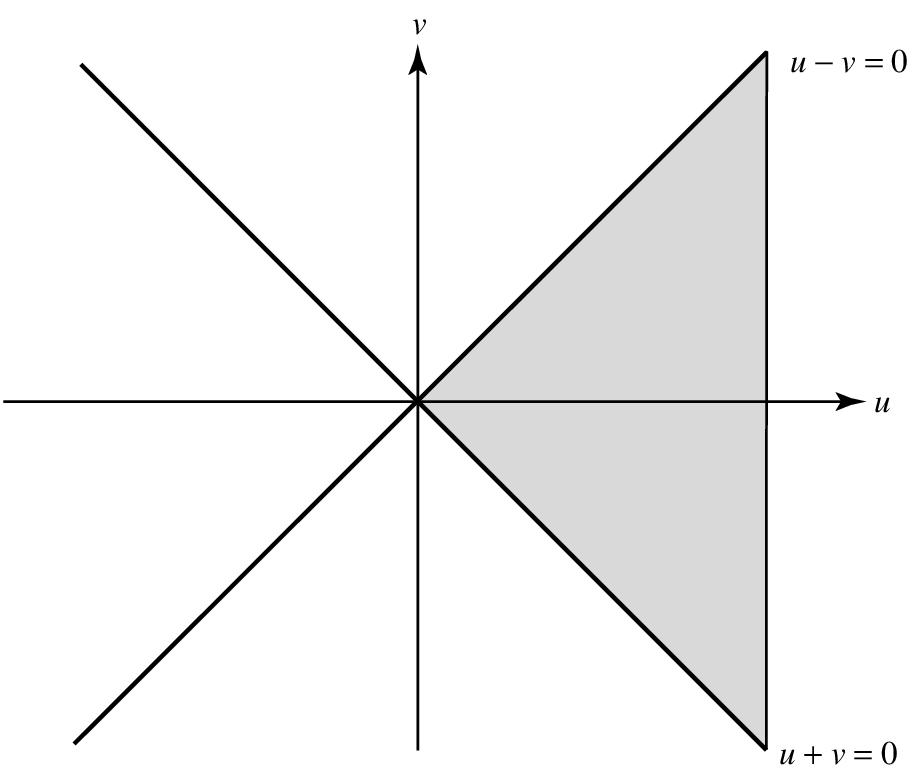
\includegraphics[width=3.1in,height=2.6in]{png/fig060301.png}
\end{center}
 \vskip6pt
 \refstepcounter{figure}
 \centerline{\bf Figure \thefigure} \label{figure:6.3.1}
 \vskip12pt

\boxit{Invertible Transformations}
\hskip-.15em
A transformation $\mathbf{F}$ is {\it one-to-one\/}, or {\it
invertible\/}, if $\mathbf{F}(\mathbf{X}_1)$ and $\mathbf{F}(\mathbf{X}_2)$ are
distinct whenever $\mathbf{X}_1$ and $\mathbf{X}_2$ are distinct points of
$D_\mathbf{F}$. In this case, we can define a function $\mathbf{G}$ on the
range
$$
R(\mathbf{F})=\set{\mathbf{U}}{\mathbf{U}=\mathbf{F}(\mathbf{X})\mbox{ for
some }\mathbf{X}\in D_\mathbf{F}}
$$
 of $\mathbf{F}$ by defining $\mathbf{G}(\mathbf{U})$
 to be the unique point in $D_\mathbf{F}$ such that
$\mathbf{F}(\mathbf{U})
=\mathbf{U}$. Then
$$
D_\mathbf{G}=R(\mathbf{F})\mbox{\quad and\quad} R(\mathbf{G})=D_\mathbf{F}.
$$
Moreover, $\mathbf{G}$ is one-to-one,
$$
\mathbf{G}(\mathbf{F}(\mathbf{X}))=\mathbf{X},\quad \mathbf{X}\in D_\mathbf{F},
$$
and
$$
\mathbf{F}(\mathbf{G}(\mathbf{U}))=\mathbf{U},\quad \mathbf{U}\in D_\mathbf{G}.
$$
We say that $\mathbf{G}$ is the {\it inverse\/} of $\mathbf{F}$, and
 write $\mathbf{G}=\mathbf{F}^{-1}$. The relation between
$\mathbf{F}$ and $\mathbf{G}$ is symmetric; that is, $\mathbf{F}$ is
also the
inverse of $\mathbf{G}$, and we  write $\mathbf{F}= \mathbf{G}^{-1}$.

\begin{example}\label{example:6.3.2}\rm  The linear transformation
\begin{equation} \label{eq:6.3.1}
\left[\begin{array}{c} u\\ v\end{array}\right]=
\mathbf{L}(x,y)=\left[\begin{array}{c} x-y\\
x+y\end{array}\right]
\end{equation}
maps $(x,y)$ to $(u,v)$, where
\begin{equation} \label{eq:6.3.2}
\begin{array}{rcl}
u\ar=x-y,\\
v\ar=x+y.\end{array}
\end{equation}
$\mathbf{L}$ is one-to-one and $R(\mathbf{L})=\R^2$, since for each
$(u,v)$ in $\R^2$ there is exactly one $(x,y)$ such that
$\mathbf{L}(x,y)=(u,v)$. This is so because the system
\eqref{eq:6.3.2}
can be solved uniquely for $(x,y)$ in terms of $(u,v)$:
\begin{equation} \label{eq:6.3.3}
\begin{array}{rcl}
x\ar=\frac{1}{2}(u+v),\\[2\jot]
y\ar=\frac{1}{2}(-u+v).\end{array}
\end{equation}
Thus,
$$
\mathbf{L}^{-1}(u,v)=\frac{1}{2}\left[\begin{array}{c}
\phantom{-}u+v\\
-u+v\end{array}\right].
$$
\end{example}

\begin{example}\label{example:6.3.3}\rm  The linear transformation
$$
\left[\begin{array}{c} u\\ v\end{array}\right]=
\mathbf{L}_1(x,y)=\left[\begin{array}{c}
\phantom{2}x+\phantom{2}y\\ 2x+2y\end{array}\right]
$$
maps $(x,y)$ onto $(u,v)$, where
\begin{equation} \label{eq:6.3.4}
\begin{array}{rcl}
u\ar=\phantom{2}x+\phantom{2}y,\\
v\ar=2x+2y.\end{array}
\end{equation}
\newpage % 397
\noindent
$\mathbf{L}_1$ is not one-to-one, since every point on the line
$$
x+y=c\mbox{\quad (constant)}
$$
is mapped onto the single point $(c,2c)$. Hence, $\mathbf{L}_1$ does not
have an inverse.
\bbox\end{example}

The crucial difference between the transformations of
Examples~\ref{example:6.3.2} and \ref{example:6.3.3} is that the matrix of
$\mathbf{L}$ is nonsingular while the matrix of  $\mathbf{L}_1$ is singular.
Thus,
$\mathbf{L}$ (see \eqref{eq:6.3.1}) can be written as
\begin{equation} \label{eq:6.3.5}
\left[\begin{array}{c} u\\ v\end{array}\right]=\left[\begin{array}{rr}
1&-1\\ 1&
1\end{array}\right]\left[\begin{array}{c} x\\ y\end{array}\right],
\end{equation}
where the matrix has the inverse
$$
\left[\begin{array}{rr}\frac{1}{2}&\frac{1}{2}\\
[3\jot]
-\frac{1}{2}&\frac{1}{2}\end{array}\right].
$$
(Verify.) Multiplying both sides of \eqref{eq:6.3.5} by this matrix yields
$$
\left[\begin{array}{rr}\frac{1}{2}&\frac{1}{2}\\
[3\jot]
-\frac{1}{2}&\frac{1}{2}\end{array}\right]
\left[\begin{array}{c} u\\ v\end{array}\right]=\left[\begin{array}{c} x\\ y\end{array}
\right],
$$
which is equivalent to \eqref{eq:6.3.3}.

Since the matrix
$$
\left[\begin{array}{cc} 1&1\\ 2&2\end{array}\right]
$$
of $\mathbf{L}_1$ is singular, \eqref{eq:6.3.4} cannot be solved
uniquely for
$(x,y)$ in terms of $(u,v)$. In fact, it cannot be solved at all
unless $v=2u$.

The following theorem settles the question of invertibility of linear
transformations from $\R^n$ to $\R^n$. We leave the proof
to you (Exercise~\ref{exer:6.3.2}).

\begin{theorem} \label{thmtype:6.3.1}
The linear transformation
$$
\mathbf{U}=\mathbf{L}(\mathbf{X})=\mathbf{A}\mathbf{X}\quad  (\R^n\to
\R^n)
$$
is invertible if and only if $\mathbf{A}$ is nonsingular$,$ in which case
$R(\mathbf{L})= \R^n$ and
$$
\mathbf{L}^{-1}(\mathbf{U})=\mathbf{A}^{-1}\mathbf{U}.
$$
\end{theorem}

\boxit{Polar Coordinates}
\hskip-.5em
We will now briefly review polar coordinates,
which we will  use in some of the following examples.

The coordinates of any point $(x,y)$ can be written in infinitely many
ways as
\begin{equation} \label{eq:6.3.6}
x=r\cos\theta,\quad y=r\sin\theta,
\end{equation}
\newpage
\noindent
where
$$
r^2=x^2+y^2
$$
and, if $r>0$, $\theta$ is the angle from the $x$-axis to the line
segment from $(0,0)$ to $(x,y)$, measured counterclockwise
(Figure~\ref{figure:6.3.2}).


\vskip1pc
 \vspace*{12pt}
\begin{center}
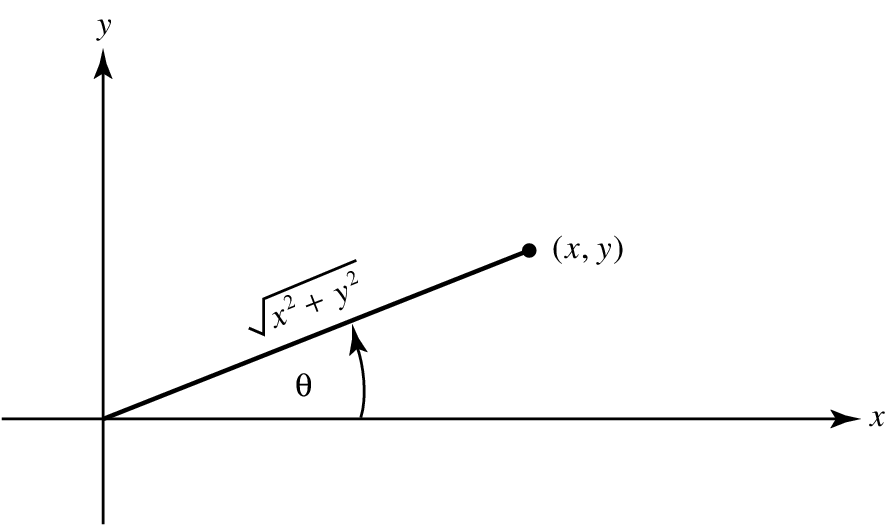
\includegraphics[width=3in,height=1.8in]{png/fig060302.png}
\end{center}
 \vskip6pt
 \refstepcounter{figure}
 \centerline{\bf Figure \thefigure} \label{figure:6.3.2}
 \vskip12pt
\vskip1pc


For each $(x,y)\ne (0,0)$ there are infinitely many values of
$\theta$, differing by integral multiples of $2\pi$, that satisfy
\eqref{eq:6.3.6}. If $\theta$ is any of these values, we say that $\theta$
is an
{\it argument} of $(x,y)$, and write
$$
\theta=\arg(x,y).
$$
By itself, this does not define a function. However, if $\phi$ is an
arbitrary fixed number, then
$$
\theta=\arg(x,y),\quad \phi\le\theta<\phi+2\pi,
$$
does define a function, since every half-open interval
$[\phi,\phi+2\pi)$ contains exactly one argument of $(x,y)$.


We do not define $\arg(0,0)$, since \eqref{eq:6.3.6} places no restriction
on $\theta$ if $(x,y)=(0,0)$ and therefore $r=0$.

The transformation
$$
\left[\begin{array}{c} r\\\theta\end{array}\right]=\mathbf{G}(x,y)=
\left[\begin{array}{c}\sqrt{x^2+y^2}\\
[3\jot]
\arg(x,y)\end{array}\right],\quad \phi\le\arg(x,y)<\phi+2\pi,
$$
is defined and one-to-one on
$$
D_\mathbf{G}=\set{(x,y)}{(x,y)\ne (0,0)},
$$
and its range is
$$
R(\mathbf{G})=\set{(r,\theta)}{ r>0,\, \phi\le\theta<\phi+2\pi}.
$$
\newpage
\noindent
For example, if $\phi=0$, then
$$
\mathbf{G}(1,1)=\left[\begin{array}{c}\sqrt{2}\\
[3\jot]
\dst{\frac{\pi}{4}}\end{array}\right],
$$
since $\pi/4$ is the unique argument of $(1,1)$ in $[0,2\pi)$. If
$\phi=\pi$, then
$$
\mathbf{G}(1,1)=\left[\begin{array}{c}\sqrt{2}\\
[3\jot]
\dst{\frac{9\pi}{4}}\end{array}\right],
$$
since $9\pi/4$ is the unique argument of $(1,1)$ in $[\pi,3\pi)$.

If $\arg(x_0,y_0)=\phi$, then $(x_0,y_0)$ is on the half-line shown in
Figure~\ref{figure:6.3.3} and  $\mathbf{G}$ is not continuous at
$(x_0,y_0)$,
since every neighborhood of $(x_0,y_0)$ contains points $(x,y)$ for
which the second component of $\mathbf{G}(x,y)$ is arbitrarily close to
$\phi+2\pi$, while the second component of $\mathbf{G}(x_0,y_0)$ is
$\phi$. We will show later, however, that $\mathbf{G}$ is continuous, in
fact, continuously differentiable, on the plane with this half-line
deleted.

 \vspace*{12pt}
\begin{center}
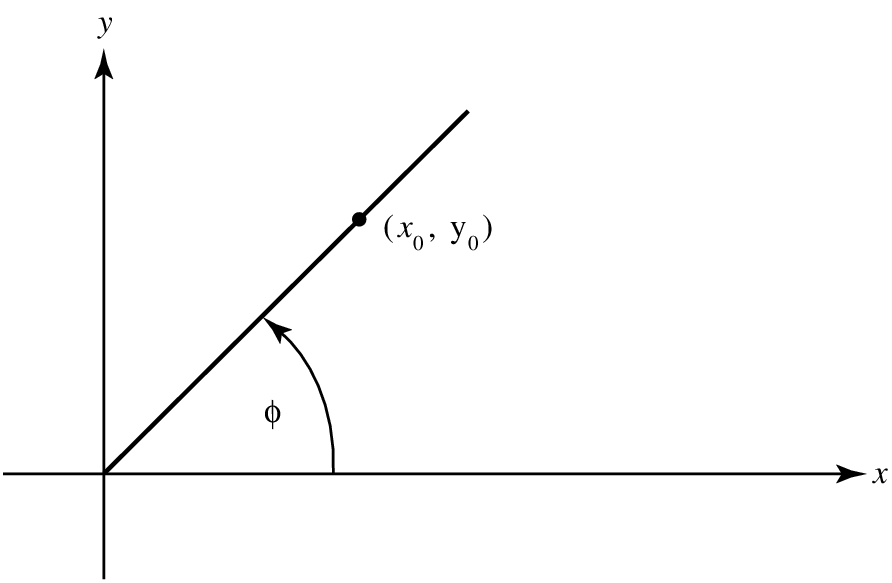
\includegraphics[width=3.05in,height=2in]{png/fig060303.png}
\end{center}
 \vskip6pt
 \refstepcounter{figure}
 \centerline{\bf Figure \thefigure} \label{figure:6.3.3}
 \vskip12pt


\boxit{Local Invertibility}
A transformation $\mathbf{F}$ may fail to be one-to-one, but be
one-to-one on a subset $S$ of $D_\mathbf{F}$. By this we mean that
$\mathbf{F}(\mathbf{X}_1)$ and $\mathbf{F}(\mathbf{X}_2)$ are
distinct whenever $\mathbf{X}_{1}$
 and $\mathbf{X}_2$ are distinct points of $S$. In this case,
$\mathbf{F}$ is not invertible, but if $\mathbf{F}_S$ is defined on
$S$ by
$$
\mathbf{F}_S(\mathbf{X})=\mathbf{F}(\mathbf{X}),\quad \mathbf{X}\in S,
$$
and left undefined for $\mathbf{X}\not\in S$, then $\mathbf{F}_S$ is
invertible. We say that $\mathbf{F}_S$ is the {\it restriction of
$\mathbf{F}$ to $S$},
and that $\mathbf{F}^{-1}_S$ is the {\it inverse of
$\mathbf{F}$ restricted to $S$}. The domain of $\mathbf{F}^{-1}_S$ is
$\mathbf{F}(S)$.
\newpage




If $\mathbf{F}$ is one-to-one on a neighborhood of $\mathbf{X}_0$, we say
that $\mathbf{F}$ is {\it locally invertible at $\mathbf{X\/}_0$}.
 If this is
true for every $\mathbf{X}_0$ in a set $S$, then $\mathbf{F}$ is {\it
locally invertible on $S$}.

\begin{example}\label{example:6.3.4}\rm
The transformation
\begin{equation} \label{eq:6.3.7}
\left[\begin{array}{c} u\\ v\end{array}\right]=\mathbf{F}(x,y)=
\left[\begin{array}{c} x^2-y^2
\\ 2xy\end{array}\right]
\end{equation}
is not one-to-one, since
\begin{equation} \label{eq:6.3.8}
\mathbf{F}(-x,-y)=\mathbf{F}(x,y).
\end{equation}
It is one-to-one on $S$ if and only if $S$ does not contain any pair
of distinct points of the form $(x_0,y_0)$ and $(-x_0,-y_0)$;
\eqref{eq:6.3.8} implies the necessity of this condition, and its
sufficiency follows from the fact that if
\begin{equation} \label{eq:6.3.9}
\mathbf{F}(x_1,y_1)=\mathbf{F}(x_0,y_0),
\end{equation}
then
\begin{equation} \label{eq:6.3.10}
(x_1,y_1)=(x_0,y_0)\mbox{\quad or\quad} (x_1,y_1)=(-x_0,-y_0).
\end{equation}
To see this, suppose that \eqref{eq:6.3.9} holds; then
\begin{eqnarray}
x^2_1-y^2_1\ar=x^2_0-y^2_0  \label{eq:6.3.11}\\
\arraytext{and}\nonumber\\
x_1y_1\ar=x_0y_0. \label{eq:6.3.12}
\end{eqnarray}
Squaring both sides of \eqref{eq:6.3.11} yields
$$
x^4_1-2x^2_1 y^2_1+y^4_1=x^4_0-2x^2_0y^2_0+y^4_0.
$$
This and \eqref{eq:6.3.12} imply that
\begin{equation} \label{eq:6.3.13}
x^4_1-x^4_0=y^4_0-y^4_1.
\end{equation}
From \eqref{eq:6.3.11},
\begin{equation} \label{eq:6.3.14}
x^2_1-x^2_0=y^2_1-y^2_0.
\end{equation}
Factoring \eqref{eq:6.3.13} yields
$$
(x^2_1-x^2_0)(x^2_1+x^2_0)=(y^2_0-y^2_1)(y^2_0+y^2_1).
$$
If either side of \eqref{eq:6.3.14} is nonzero, we can cancel  to obtain
$$
x^2_1+x^2_0=-y^2_0-y^2_1,
$$
which implies that $x_0=x_1=y_0=y_1=0$, so \eqref{eq:6.3.10} holds in
this case. On the other hand, if both sides of \eqref{eq:6.3.14} are zero,
then
$$
x_1=\pm x_0,\quad y_1=\pm y_0.
$$
From \eqref{eq:6.3.12}, the same sign must be chosen in these equalities,
which proves that \eqref{eq:6.3.8} implies \eqref{eq:6.3.10} in this case
also.

We now see, for example, that $\mathbf{F}$ is one-to-one on every
set $S$ of the form
$$
S=\set{(x,y)}{ax+by>0},
$$
where $a$ and $b$ are constants, not both zero. Geometrically, $S$ is
an open half-plane; that is, the set of points on one side of, but
not on, the line
$$
ax+by=0
$$
(Figure~\ref{figure:6.3.4}). Therefore, $\mathbf{F}$ is locally invertible at
every $\mathbf{X}_0\ne (0,0)$, since every such point lies in a
half-plane of this form. However, $\mathbf{F}$ is not locally invertible
at
$(0,0)$. (Why not?) Thus, $\mathbf{F}$ is locally invertible on the
entire plane with $(0,0)$ removed.

 \vspace*{12pt}
\begin{center}
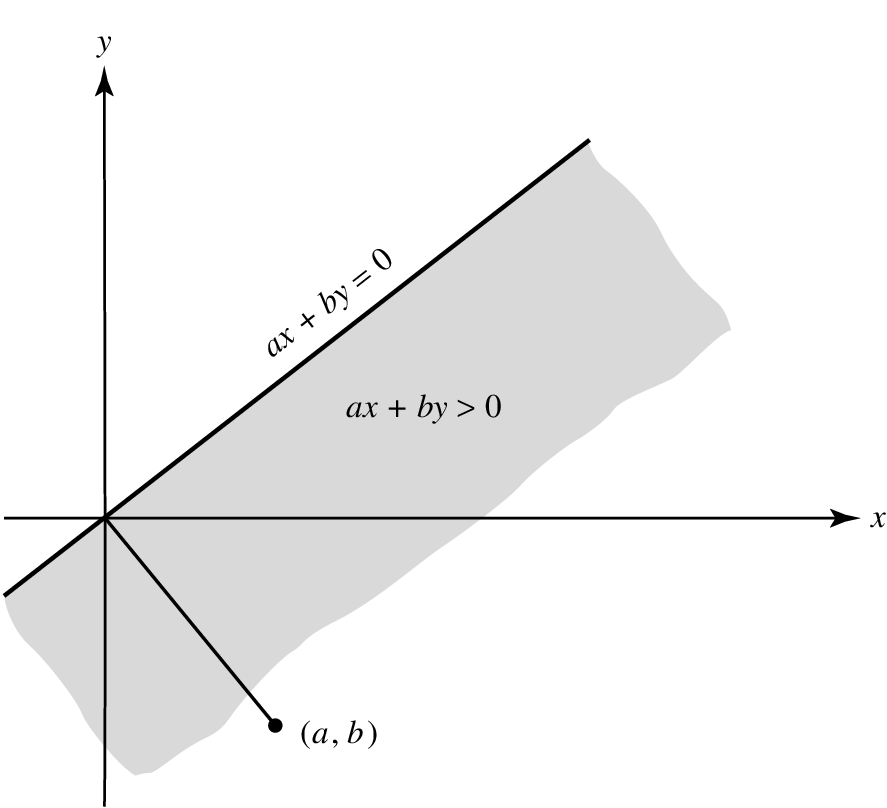
\includegraphics[width=3in,height=2.65in]{png/fig060304.png}
\end{center}
 \vskip6pt
 \refstepcounter{figure}
 \centerline{\bf Figure \thefigure} \label{figure:6.3.4}
 \vskip12pt

It is instructive to find $\mathbf{F}^{-1}_S$ for a specific choice of $S$.
Suppose that $S$ is the open right half-plane:
\begin{equation} \label{eq:6.3.15}
S=\set{(x,y)}{x>0}.
\end{equation}
Then $\mathbf{F}(S)$ is the entire $uv$-plane except for the nonpositive
$u$ axis. To see this, note that every point in $S$ can be written in
polar coordinates as
$$
x=r\cos\theta,\quad y=r\sin\theta,\quad r>0,\quad-\frac{\pi}{
2}<\theta<\frac{\pi}{2}.
$$
Therefore, from \eqref{eq:6.3.7}, $\mathbf{F}(x,y)$ has coordinates $(u,v)$, where
\begin{eqnarray*}
u\ar=x^2-y^2=r^2(\cos^2\theta-\sin^2\theta)=r^2\cos2\theta,\\
v\ar=2xy=2r^2\cos\theta\sin\theta=r^2\sin2\theta.
\end{eqnarray*}
\newpage
\noindent
 Every point in the $uv$-plane can be written in polar coordinates
as
$$
u=\rho\cos\alpha,\quad v=\rho\sin\alpha,
$$
where either $\rho=0$ or
$$
\rho=\sqrt{u^2+v^2}>0,\quad-\pi\le\alpha<\pi,
$$
and the points for which $\rho=0$ or $\alpha=-\pi$ are of the form
$(u,0)$, with $u\le0$ (Figure~\ref{figure:6.3.5}). If $(u,v)=\mathbf{F}(x,y)$
for some $(x,y)$ in  $S$, then \eqref{eq:6.3.15} implies that $\rho>0$ and
$-\pi<\alpha<\pi$. Conversely, any point in the $uv$-plane with polar
coordinates $(\rho,\alpha)$ satisfying these conditions is the image
under $\mathbf{F}$ of the point
$$
(x,y)=(\rho^{1/2}\cos\alpha/2,\rho^{1/2}\sin\alpha/2)\in S.
$$
 Thus,
$$
\mathbf{F}^{-1}_S(u,v)=\left[\begin{array}{c}
(u^2+v^2)^{1/4}\cos(\arg(u,v)/2)\\
[3\jot]
(u^2+v^2)^{1/4}\sin(\arg (u,v)/2\end{array}\right],
\quad-\pi<\arg (u,v)<\pi.
$$

 \vspace*{12pt}
\begin{center}
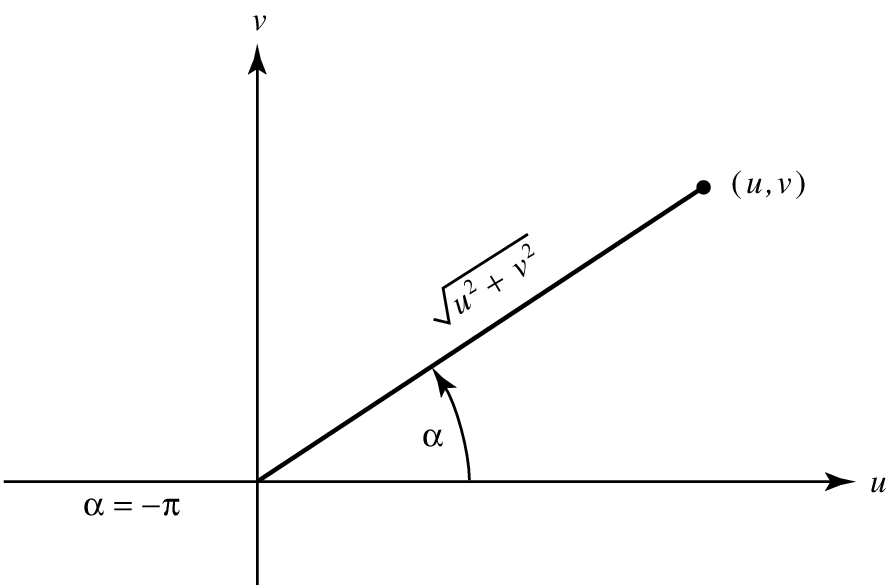
\includegraphics[width=3in,height=2.05in]{png/fig060305.png}
\end{center}
 \vskip6pt
 \refstepcounter{figure}
 \centerline{\bf Figure \thefigure} \label{figure:6.3.5}
 \vskip12pt

Because of \eqref{eq:6.3.8}, $\mathbf{F}$ also maps the open left half-plane
$$
S_1=\set{(x,y)}{x<0}
$$
onto $\mathbf{F}(S)$, and
\begin{eqnarray*}
\mathbf{F}^{-1}_{S_1}(u,v)\ar=\left[\begin{array}{c}
 (u^2+v^2)^{1/4}\cos
(\arg(u,v)/2)\\
[3\jot]
(u^2+v^2)^{1/4}\sin(\arg(u,v)/2)\end{array}\right],
\quad\pi<\arg (u,v)<3\pi,\\
\ar=-\mathbf{F}^{-1}_S(u,v).
\end{eqnarray*}
\end{example}



\begin{example}\label{example:6.3.5}\rm  The transformation
\begin{equation} \label{eq:6.3.16}
\left[\begin{array}{c} u\\ v\end{array}\right]=
\mathbf{F}(x,y)=\left[\begin{array}{c} e^x\cos
y\\ e^x\sin y\end{array}\right]
\end{equation}
is not one-to-one, since
\begin{equation} \label{eq:6.3.17}
\mathbf{F}(x,y+2k\pi)=\mathbf{F}(x,y)
\end{equation}
if $k$ is any integer. This transformation  is one-to-one on a set $S$
if and only if
$S$ does not contain any pair of points $(x_0,y_0)$ and
$(x_0,y_0+2k\pi)$, where $k$ is a nonzero integer. This condition is
necessary because of \eqref{eq:6.3.17}; we leave it to you to show that
it is sufficient (Exercise~\ref{exer:6.3.8}).
Therefore,  for example,  $\mathbf{F}$ is one-to-one on
\begin{equation} \label{eq:6.3.18}
S_\phi=\set{(x,y)}{-\infty<x<\infty,\, \phi\le y<\phi+2\pi}
\end{equation}
where $\phi$ is arbitrary. Geometrically, $S_\phi$ is the infinite
strip bounded by the lines $y=\phi$ and $y=\phi+2\pi$. The lower
boundary is in $S_\phi$, but the upper is not (Figure~\ref{figure:6.3.6}).
Since every point is in the interior of some such strip, $\mathbf{F}$ is
locally invertible on the entire plane.

 \vspace*{-12pt}
\begin{center}
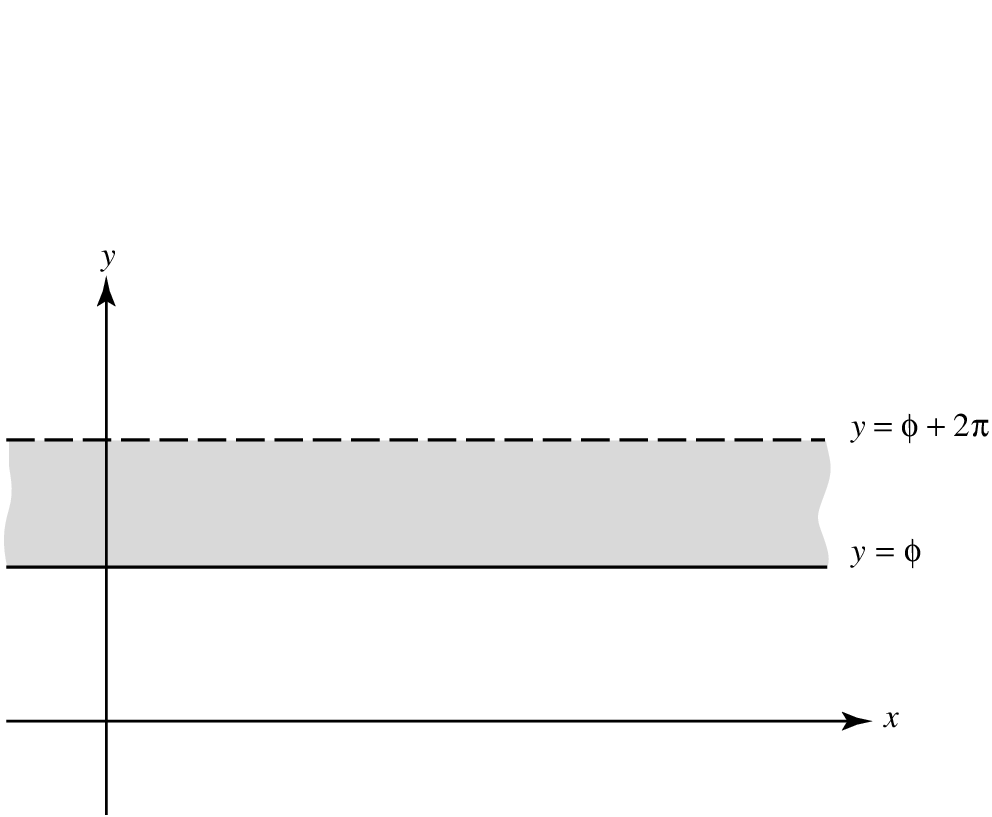
\includegraphics[width=3.3in,height=1.95in]{png/fig060306.png}
\end{center}
 \vskip6pt
 \refstepcounter{figure}
 \centerline{\bf Figure \thefigure} \label{figure:6.3.6}
 \vskip12pt


The range of $\mathbf{F}_{S_\phi}$ is the entire $uv$-plane except
the origin, since if $(u,v)\ne (0,0)$, then $(u,v)$ can be written
uniquely as
$$
\left[\begin{array}{c} u\\ v\end{array}\right]=
\left[\begin{array}{c}\rho\cos\alpha
\\\rho\sin\alpha\end{array}\right],
$$
where
$$
\rho>0,\quad\phi\le\alpha<\phi+2\pi,
$$
so $(u,v)$ is the image under $\mathbf{F}$ of
$$
(x,y)=(\log\rho,\alpha)\in S.
$$
 The origin is not in $R(\mathbf{F})$, since
$$
|\mathbf{F}(x,y)|^2=(e^x\cos y)^2+(e^x\sin y)^2=e^{2x}\ne0.
$$
\newpage

Finally,
$$
\mathbf{F}^{-1}_{S_\phi}(u,v)=\left[\begin{array}{c}\log(u^2+v^2)^{1/2}\\
[3\jot]
\arg(u,v)\end{array}\right],\quad\phi\le\arg(u,v)<\phi+2\pi.
$$
The domain of $\mathbf{F}_{S_\phi}^{-1}$ is the entire $uv$-plane
except for
$(0,0)$.
\end{example}




\vspace*{-1pc}
\boxit{Regular Transformations}
The question of invertibility of an arbitrary transformation $\mathbf{F}:
\R^n\to \R^n$ is too general to have a useful answer.
However, there is a useful and easily applicable sufficient condition
which implies that one-to-one restrictions of continuously
differentiable transformations have continuously differentiable
inverses.

To motivate our study of this question, let us first consider
 the linear transformation
$$
\mathbf{F}(\mathbf{X})=\mathbf{A}\mathbf{X}=\left[\begin{array}{cccc}
a_{11}&a_{12}&\cdots&a_{1n}\\
a_{21}&a_{22}&\cdots&a_{2n}\\\vdots&\vdots&\ddots&\vdots\\
a_{n1}&a_{n2}&\cdots&a_{nn}\end{array}\right]
\left[\begin{array}{c} x_1\\ x_2\\\vdots\\ x_n\end{array}\right].
$$
From Theorem~\ref{thmtype:6.3.1}, $\mathbf{F}$ is invertible if and only if
$\mathbf{A}$ is nonsingular, in which case $R(\mathbf{F})=\R^n$ and
$$
\mathbf{F}^{-1}(\mathbf{U})=\mathbf{A}^{-1}\mathbf{U}.
$$
Since $\mathbf{A}$ and $\mathbf{A}^{-1}$ are the differential matrices of
$\mathbf{F}$ and $\mathbf{F}^{-1}$, respectively, we can say that a linear
transformation is invertible if and only if its differential matrix
$\mathbf{F}'$ is nonsingular, in which case the differential matrix of
$\mathbf{F}^{-1}$ is given by
$$
(\mathbf{F}^{-1})'=(\mathbf{F}')^{-1}.
$$
Because of this, it is tempting to conjecture that if $\mathbf{F}:
\R^n\to \R^n$ is continuously differentiable
 and $\mathbf{A}'(\mathbf{X})$
 is nonsingular, or, equivalently, $J\mathbf{F}(\mathbf{X})\ne0$, for
$\mathbf{X}$ in a set $S$, then $\mathbf{F}$ is one-to-one on $S$. However,
this is false. For example, if
$$
\mathbf{F}(x,y)=\left[\begin{array}{c} e^x\cos y\\ e^x\sin
y\end{array}\right],
$$
then
\begin{equation} \label{eq:6.3.19}
J\mathbf{F}(x,y)=\left|\begin{array}{cr} e^x\cos y&-e^x\sin y\\
e^x\sin y&e^x\cos y\end{array}\right|=e^{2x}\ne0,
\end{equation}
but $\mathbf{F}$ is not one-to-one on $\R^2$
(Example~\ref{example:6.3.5}). The best that can be said in general is
that if $\mathbf{F}$ is continuously differentiable and
 $J\mathbf{F}(\mathbf{X})
\ne0$ in an open set $S$, then $\mathbf{F}$ is locally invertible on
$S$, and the local inverses are continuously differentiable. This is
part of the inverse function theorem, which we will prove presently.
First, we need the following definition.

\newpage


\begin{definition} \label{thmtype:6.3.2}
A transformation $\mathbf{F}: \R^n\to \R^n$ is
{\it regular\/} on an open set $S$ if $\mathbf{F}$ is one-to-one and
continuously
differentiable on $S$, and $J\mathbf{F}(\mathbf{X})\ne0$ if $\mathbf{X}\in S$.
We will also say that $\mathbf{F}$
 is regular on an arbitrary  set $S$ if
$\mathbf{F}$ is regular on an open set containing $S$.
\end{definition}

\begin{example}\label{example:6.3.6}\rm
If
$$
\mathbf{F}(x,y)=\left[\begin{array}{c} x-y\\ x+y\end{array}\right]
$$
(Example~\ref{example:6.3.2}), then
$$
J\mathbf{F}(x,y)=\left|\begin{array}{cr} 1&-1\\ 1&1\end{array}\right|=2,
$$
so $\mathbf{F}$ is one-to-one on $\R^2$. Hence, $\mathbf{F}$ is
regular on $\R^2$.

If
$$
 \mathbf{F}(x,y)=\left[\begin{array}{c} \phantom{2}x+\phantom{2}y\\
2x+2y\end{array}\right]
$$
(Example~\ref{example:6.3.3}), then
$$
J\mathbf{F}(x,y)=\left|\begin{array}{cc} 1&1\\ 2&2\end{array}\right|=0,
$$
so $\mathbf{F}$ is not regular on any subset of $\R^2$.

If
$$
\mathbf{F}(x,y)=\left[\begin{array}{c} x^2-y^2\\ 2xy\end{array}\right]
$$
(Example~\ref{example:6.3.4}), then
$$
J\mathbf{F}(x,y)=\left|\begin{array}{cr} 2x&-2y\\ 2y&2x\end{array}\right|
=2(x^2+y^2),
$$
so $\mathbf{F}$ is regular on any open set $S$ on which $\mathbf{F}$ is
one-to-one,
provided that $(0,0)\not\in S$. For example, $\mathbf{F}$ is regular on
the open half-plane $\set{(x,y)}{x>0}$, since we saw in
Example~\ref{example:6.3.4} that $\mathbf{F}$ is one-to-one on this
half-plane.

If
$$
\mathbf{F}(x,y)=\left[\begin{array}{c} e^x\cos y\\ e^x\cos y\end{array}\right]
$$
(Example~\ref{example:6.3.5}), then $J\mathbf{F}(x,y)=e^{2x}$ (see
\eqref{eq:6.3.19}), so $\mathbf{F}$ is regular on any open set on which
it is one-to-one. The interior of $S_\phi$ in \eqref{eq:6.3.18}
is an example of such a set.
\end{example}

\begin{theorem} \label{thmtype:6.3.3}
Suppose that $\mathbf{F}: \R^n\to \R^n$ is regular on an open
set $S,$ and let $\mathbf{G}=\mathbf{F}^{-1}_S.$ Then $\mathbf{F}(S)$ is
open$,$
$\mathbf{G}$ is continuously differentiable on $\mathbf{F}(S),$ and
$$
\mathbf{G}'(\mathbf{U})=(\mathbf{F}'(\mathbf{X}))^{-1},
\mbox{\quad where\quad}\mathbf{U}=\mathbf{F}(\mathbf{X}).
$$
Moreover$,$ since $\mathbf{G}$ is one-to-one on $\mathbf{F}(S),$
 $\mathbf{G}$ is regular on $\mathbf{F}(S).$
\end{theorem}
 \newpage

\proof
 We first  show that if $\mathbf{X}_{0} \in S$,
  then a neighborhood of $\mathbf{F}(\mathbf{X}_0)$ is in
$\mathbf{F}(S)$.
This implies that $\mathbf{F}(S)$ is open.

Since $S$ is open, there is a $\rho>0$ such that
 $\overline{B_\rho(\mathbf{X}_0)}\subset S$. Let $B$
be the boundary of $B_\rho(\mathbf{X}_0)$; thus,
\begin{equation} \label{eq:6.3.20}
B=\set\mathbf{X}{|\mathbf{X}-\mathbf{X}_0|=\rho}.
\end{equation}
The function
$$
\sigma(\mathbf{X})=|\mathbf{F}(\mathbf{X})-\mathbf{F}(\mathbf{X}_0)|
$$
is continuous on $S$ and therefore on $B$, which is compact. Hence,
by Theorem~\ref{thmtype:5.2.12}, there is a point $\mathbf{X}_1$
in $B$ where $\sigma(\mathbf{X})$ attains its minimum value, say $m$, on
$B$. Moreover, $m>0$, since $\mathbf{X}_1\ne\mathbf{X}_0$ and $\mathbf{F}$ is
one-to-one on $S$. Therefore,
\begin{equation} \label{eq:6.3.21}
|\mathbf{F}(\mathbf{X})-\mathbf{F}(\mathbf{X}_0)|\ge m>0\mbox{\quad if\quad}
|\mathbf{X}-\mathbf{X}_0|=\rho.
\end{equation}
The set
$$
\set{\mathbf{U}}{|\mathbf{U}-\mathbf{F}(\mathbf{X}_0)|<m/2}
$$
is  a neighborhood of $\mathbf{F}(\mathbf{X}_0)$. We will show that
it is a subset of $\mathbf{F}(S)$. To see this, let $\mathbf{U}$ be a fixed
point in this set; thus,
\begin{equation} \label{eq:6.3.22}
|\mathbf{U}-F(\mathbf{X}_0)|<m/2.
\end{equation}
Consider the function
$$
\sigma_1(\mathbf{X})=|\mathbf{U}-\mathbf{F}(\mathbf{X})|^2,
$$
which is continuous on $S$. Note that
\begin{equation} \label{eq:6.3.23}
\sigma_1(\mathbf{X})\ge\frac{m^2}{4}\mbox{\quad if \quad}
|\mathbf{X}-\mathbf{X}_0|=\rho,
\end{equation}
since if $|\mathbf{X}-\mathbf{X}_0|=\rho$, then
\begin{eqnarray*}
|\mathbf{U}-\mathbf{F}(\mathbf{X})|\ar=|(\mathbf{U}-\mathbf{F}(\mathbf{X}_0))
+(\mathbf{F}(\mathbf{X}_0)-\mathbf{F}(\mathbf{X}))| \\
\ar\ge  \big||\mathbf{F}(\mathbf{X}_0)-\mathbf{F}(\mathbf{X})|
-|\mathbf{U}-\mathbf{F}(\mathbf{X}_0)|\big|\\
\ar\ge m-\frac{m}{2}=\frac{m}{2},
\end{eqnarray*}
from  \eqref{eq:6.3.21} and \eqref{eq:6.3.22}.

Since  $\sigma_1$ is continuous on $S$,
$\sigma_1$ attains a minimum value
$\mu$
on the compact set $\overline{B_\rho(\mathbf{X}_0)}$
 (Theorem~\ref{thmtype:5.2.12}); that is, there
is an $\overline{\mathbf{X}}$ in $\overline{B_\rho(\mathbf{X}_0)}$ such that
$$
\sigma_1(\mathbf{X})\ge\sigma_1(\overline{\mathbf{X}})=\mu,
\quad\mathbf{X}\in\overline{B_\rho (\mathbf{X}_0)}.
$$
Setting $\mathbf{X}=\mathbf{X}_0$, we conclude from this and \eqref{eq:6.3.22} that
\vspace*{-3pt}
$$
\sigma_1(\overline{\mathbf{X}})=\mu\le\sigma_1(\mathbf{X}_0)<\frac{m^2}{4}.
$$
Because of \eqref{eq:6.3.20} and \eqref{eq:6.3.23}, this rules out the
possibility
that $\overline{\mathbf{X}}\in B$, so  $\overline{\mathbf{X}}\in
B_\rho(\mathbf{X}_0)$.
\enlargethispage{-.12\baselineskip}

\newpage

\enlargethispage{\baselineskip}

Now we want to show that $\mu=0$; that is, $\mathbf{U}=
\mathbf{F}(\overline{\mathbf{X}})$. To this end, we note that
$\sigma_1(\mathbf{X})$ can be written as
$$
\sigma_1(\mathbf{X})=\sum^n_{j=1}(u_j-f_j(\mathbf{X}))^2,
$$
\vspace*{3pt}
\noindent \hskip-.4em so $\sigma_1$   is differentiable on
$B_p(\mathbf{X}_{0})$.
 Therefore, the first
partial derivatives of $\sigma_1$ are all zero  at the local minimum
point
$\overline{\mathbf{X}}$ (Theorem~\ref{thmtype:5.3.11}), so
\vskip3pt
$$
\sum^n_{j=1}\frac{\partial f_j(\overline{\mathbf{X}})}{\partial x_i}
(u_j-f_j(\overline{\mathbf{X}}))=0,\quad 1\le i\le n,
$$
 or, in matrix form,
$$
\mathbf{F}'(\overline{\mathbf{X}})(\mathbf{U}-\mathbf{F}(\overline{\mathbf{X}}))=0.
$$
Since $\mathbf{F}'(\overline{\mathbf{X}})$ is nonsingular this
implies that
$\mathbf{U}= \mathbf{F}(\overline{\mathbf{X}})$
(Theorem~\ref{thmtype:6.1.13}). Thus, we have shown that every
$\mathbf{U}$ that satisfies \eqref{eq:6.3.22} is in
$\mathbf{F}(S)$. Therefore, since
$\mathbf{X}_0$ is an arbitrary point of $S$,
$\mathbf{F}(S)$ is open.

Next, we show that $\mathbf{G}$ is continuous on $\mathbf{F}(S)$. Suppose that
$\mathbf{U}_0\in\mathbf{F}(S)$ and $\mathbf{X}_0$ is the unique point in
$S$ such that $\mathbf{F}(\mathbf{X}_0)=\mathbf{U}_0$.
  Since $\mathbf{F}'(\mathbf{X}_{0})$
 is invertible,
 Lemma~\ref{thmtype:6.2.6} implies that  there is a $\lambda>0$
and an open neighborhood $N$ of $\mathbf{X}_0$ such that $N\subset S$ and
\begin{equation} \label{eq:6.3.24}
|\mathbf{F}(\mathbf{X})-\mathbf{F}(\mathbf{X}_0)|\ge\lambda |\mathbf{X}-\mathbf{X}_0|
\mbox{\quad if\quad}\mathbf{X}\in N.
\end{equation}
(Exercise~\ref{exer:6.2.18} also implies this.) Since $\mathbf{F}$
satisfies the hypotheses of the present theorem on $N$, the first part
of this proof shows that $\mathbf{F}(N)$ is an open set containing
$\mathbf{U}_0=\mathbf{F} (\mathbf{X}_0)$. Therefore, there is a
$\delta>0$ such that
$\mathbf{X}=\mathbf{G}(\mathbf{U})$ is in $N$ if $\mathbf{U}\in
B_\delta(\mathbf{U}_{0})$.
 Setting $\mathbf{X}=\mathbf{G}(\mathbf{U})$ and $\mathbf{X}_0 =
\mathbf{G}(\mathbf{U}_0)$ in \eqref{eq:6.3.24} yields
$$
|\mathbf{F}(\mathbf{G}(\mathbf{U}))-\mathbf{F}(\mathbf{G}(\mathbf{U}_0))
|\ge\lambda
|\mathbf{G}(\mathbf{U})-\mathbf{G}(\mathbf{U}_0)|\mbox{\quad if \quad}
\mathbf{U}\in B_\delta (\mathbf{U}_0).
$$
Since $\mathbf{F}(\mathbf{G}(\mathbf{U}))=\mathbf{U}$, this can be rewritten as
\begin{equation} \label{eq:6.3.25}
|\mathbf{G}(\mathbf{U})-\mathbf{G}(\mathbf{U}_0)|\le\frac{1}{\lambda} |\mathbf{U}-
\mathbf{U}_0|\mbox{\quad if\quad}\mathbf{U}\in B_\delta(\mathbf{U}_0),
\end{equation}
which means that $\mathbf{G}$ is continuous at $\mathbf{U}_0$.
Since $\mathbf{U}_0$ is an arbitrary point in $\mathbf{F}(S)$, it follows
that $\mathbf{G}$ is continous on $\mathbf{F}(S)$.

We will now show that $\mathbf{G}$ is differentiable at $\mathbf{U}_0$.
Since
$$
\mathbf{G}(\mathbf{F}(\mathbf{X}))=\mathbf{X},\quad\mathbf{X}\in S,
$$
the chain rule (Theorem~\ref{thmtype:6.2.8}) implies that
{\it if\/} $\mathbf{G}$ is differentiable at $\mathbf{U}_0$, then
$$
\mathbf{G}'(\mathbf{U}_0)\mathbf{F}'(\mathbf{X}_0)=\mathbf{I}
$$
\newpage

\noindent
(Example~\ref{example:6.2.3}).
 Therefore, if
$\mathbf{G}$ is differentiable at $\mathbf{U}_0$, the  differential matrix
of $\mathbf{G}$
must be
$$
\mathbf{G}'(\mathbf{U}_0)=[\mathbf{F}'(\mathbf{X}_0)]^{-1},
$$
so to show that $\mathbf{G}$ is differentiable at
$\mathbf{U}_0$, we must show that if
\begin{equation} \label{eq:6.3.26}
\mathbf{H}(\mathbf{U})=
\frac{\mathbf{G}(\mathbf{U})-\mathbf{G}(\mathbf{U}_0)-
[\mathbf{F}'(\mathbf{X}
_0)]^{-1} (\mathbf{U}-\mathbf{U}_0)}{ |\mathbf{U}-\mathbf{U}_0|}\quad
(\mathbf{U}\ne\mathbf{U}_0),
\end{equation}
then
\begin{equation} \label{eq:6.3.27}
\lim_{\mathbf{U}\to\mathbf{U}_0}\mathbf{H}(\mathbf{U})=\mathbf{0}.
\end{equation}

Since $\mathbf{F}$  is one-to-one on $S$ and $\mathbf{F}
(\mathbf{G}(\mathbf{U}))
=\mathbf{U}$, it follows that if $\mathbf{U}\ne\mathbf{U}_0$,  then
$\mathbf{G}(\mathbf{U})\ne\mathbf{G}(\mathbf{U}_0)$. Therefore, we can multiply
the numerator and denominator of \eqref{eq:6.3.26}
 by $|\mathbf{G}(\mathbf{U})
-\mathbf{G}(\mathbf{U}_0)|$ to obtain
$$
\begin{array}{rcl}
\mathbf{H}(\mathbf{U})\ar=
\dst\frac{|\mathbf{G}(\mathbf{U})-\mathbf{G}(\mathbf{U}_{0}|}
{|\mathbf{U}-\mathbf{U}_0|}
\left(\frac{\mathbf{G}(\mathbf{U})-\mathbf{G}
(\mathbf{U}_0)-
\left[\mathbf{F}'(\mathbf{X}_{0})
\right]^{-1}(\mathbf{U}-\mathbf{U}_0)}
{|\mathbf{G}(\mathbf{U})-\mathbf{G}(\mathbf{U}_0)|}\right)\\\\
\ar=-\dst\frac{|\mathbf{G}(\mathbf{U})-\mathbf{G}(\mathbf{U}_0)|}{
|\mathbf{U}-\mathbf{U}_0|}
\left[\mathbf{F}'(\mathbf{X}_0)\right]^{-1}
\left(\frac{\mathbf{U}-\mathbf{U}_0-\mathbf{F}'(\mathbf{X}_0)
(\mathbf{G}(\mathbf{U})-\mathbf{G}(\mathbf{U}_0))
}{|\mathbf{G}(\mathbf{U})-\mathbf{G}(\mathbf{U}_0)|}\right)
\end{array}
$$
 if $0<|\mathbf{U}-\mathbf{U}_0|<\delta$.
Because of \eqref{eq:6.3.25},  this implies that
$$
|\mathbf{H}(\mathbf{U})|\le\frac{1}{\lambda}
\|[\mathbf{F}'(\mathbf{X}_0)]^{-1}\|
\left|\frac{\mathbf{U}-\mathbf{U}_0-\mathbf{F}'(\mathbf{X}_0)
(\mathbf{G}(\mathbf{U})-\mathbf{G}(\mathbf{U}_0))}{
|\mathbf{G}(\mathbf{U})-\mathbf{G}(\mathbf{U}_0)|}\right|
$$
 if $0<|\mathbf{U}-\mathbf{U}_0|<\delta$.
Now let
$$
\mathbf{H}_1(\mathbf{U})=\frac{\mathbf{U}-\mathbf{U}_0-\mathbf{F}'(\mathbf{X}_0)
(\mathbf{G}(\mathbf{U})-\mathbf{G}(\mathbf{U}_0))}{
|\mathbf{G}(\mathbf{U})-\mathbf{G}(\mathbf{U}_0)|}
$$
To complete the proof of \eqref{eq:6.3.27}, we must show that
\begin{equation} \label{eq:6.3.28}
\lim_{\mathbf{U}\to\mathbf{U}_0}\mathbf{H}_1(\mathbf{U})=\mathbf{0}.
\end{equation}
Since $\mathbf{F}$ is differentiable at $\mathbf{X}_0$, we know that if
$$
\mathbf{H}_2(\mathbf{X})=
\lim_{\mathbf{X}\to\mathbf{X}_0}
\frac{\mathbf{F}(\mathbf{X})-\mathbf{F}(\mathbf{X}_0)-\mathbf{F}'(\mathbf{X}_0)
(\mathbf{X}-\mathbf{X}_0)}{
|\mathbf{X}-\mathbf{X}_0|},
$$
then
\begin{equation} \label{eq:6.3.29}
\lim_{\mathbf{X}\to\mathbf{X}_0}\mathbf{H}_2(\mathbf{X})=\mathbf{0}.
\end{equation}
Since $\mathbf{F}(\mathbf{G}(\mathbf{U}))=\mathbf{U}$ and $\mathbf{X}_0=
\mathbf{G}(\mathbf{U}_0)$,
$$
\mathbf{H}_1(\mathbf{U})=\mathbf{H}_2(\mathbf{G}(\mathbf{U})).
$$
\newpage
\noindent
Now suppose that $\epsilon>0$. From \eqref{eq:6.3.29}, there is a
$\delta_1>0$ such that
\begin{equation} \label{eq:6.3.30}
|\mathbf{H}_2(\mathbf{X})|<\epsilon\mbox{\quad if \quad} 0<
|\mathbf{X}-\mathbf{X}_{0}|
=|\mathbf{X}-\mathbf{G}(\mathbf{U}_0)|<\delta_1.
\end{equation}
Since $\mathbf{G}$ is continuous at $\mathbf{U}_0$, there is a
$\delta_2\in(0,\delta)$ such that
$$
|\mathbf{G}(\mathbf{U})-\mathbf{G}(\mathbf{U}_0)|<\delta_1\mbox{\quad if \quad}
0<|\mathbf{U}-\mathbf{U}_0|<\delta_2.
$$
This and \eqref{eq:6.3.30} imply
that
$$
|\mathbf{H}_1(\mathbf{U})|=|\mathbf{H}_2(\mathbf{G}(\mathbf{U}))|<\epsilon
\mbox{\quad if \quad} 0<|\mathbf{U}-\mathbf{U}_0|<\delta_2.
$$
Since this implies
\eqref{eq:6.3.28},  $\mathbf{G}$
is differentiable at $\mathbf{X}_0$.


Since $\mathbf{U}_0$ is an arbitrary member of $\mathbf{F}(N)$, we
can now drop the zero subscript and conclude that $\mathbf{G}$
is continuous and differentiable on $\mathbf{F}(N)$, and
$$
\mathbf{G}'(\mathbf{U})=[\mathbf{F}'(\mathbf{X})]^{-1},\quad\mathbf{U}\in\mathbf{F}(N).
$$
To see that $\mathbf{G}$ is  \emph{continuously differentiable} on
$\mathbf{F}(N)$, we observe that by
Theorem~\ref{thmtype:6.1.14}, each
entry of $\mathbf{G}'(\mathbf{U})$ (that is, each partial derivative
$\partial g_i(\mathbf{U})/\partial u_j$, $1\le i, j\le n$) can be written
as the ratio, with nonzero denominator, of determinants with
entries of the form
\begin{equation} \label{eq:6.3.31}
\frac{\partial f_r(\mathbf{G}(\mathbf{U}))}{\partial x_s}.
\end{equation}
Since $\partial f_r/\partial x_s$ is continuous on $N$ and $\mathbf{G}$
is continuous on $\mathbf{F}(N)$, Theorem~\ref{thmtype:5.2.10}
implies that \eqref{eq:6.3.31} is continuous on $\mathbf{F}(N)$. Since a
determinant is a continuous function of its entries, it now follows
that the entries of $\mathbf{G}'(\mathbf{U})$ are continuous on
$\mathbf{F}(N)$.
\bbox

\boxit{Branches of the Inverse}
\hskip-.4em
If $\mathbf{F}$ is regular on an open set $S$, we say that
$\mathbf{F}^{-1}_S$ is a {\it branch of\/} $\mathbf{F}^{-1}$. (This is
a convenient
terminology but is not meant to imply that $\mathbf{F}$ actually has an
inverse.)
From this  definition, it is possible to define a branch of
$\mathbf{F}^{-1}$ on a
set $T \subset R(\mathbf{F})$ if and only if $T=\mathbf{F}(S)$, where
$\mathbf{F}$ is regular on $S$. There may be open subsets of
$R(\mathbf{F})$ that
do not have this property, and therefore no branch of $\mathbf{F}^{-1}$
can be defined on them. It is also possible that $T=\mathbf{F}(S_1)=
\mathbf{F}(S_2)$, where $S_1$ and $S_2$ are distinct subsets of
$D_\mathbf{F}$.
In this case, more than one branch of $\mathbf{F}^{-1}$ is defined on
$T$.
Thus, we saw in Example~\ref{example:6.3.4}
 that two branches of
$\mathbf{F}^{-1}$ may be defined on a set $T$. In
Example~\ref{example:6.3.5}
infinitely many branches of $\mathbf{F}^{-1}$ are defined on the same
set.

It is  useful to define branches of the argument
To do this, we think of the relationship between polar and rectangular
coordinates in terms of the transformation
\begin{equation} \label{eq:6.3.32}
\left[\begin{array}{c} x\\ y\end{array}\right]=\mathbf{F}(r,\theta)=
\left[\begin{array}{c} r
\cos\theta\\ r\sin\theta\end{array}\right],
\end{equation}
where for the moment we regard $r$ and $\theta$ as rectangular
coordinates of a point in an $r\theta$-plane. Let $S$ be an open
subset of the right half of this plane (that is,
$S\subset\set{(r,\theta)}{r>0}$)
\newpage
\noindent
 that does not contain any pair of
points $(r,\theta)$ and $(r,\theta+2k\pi)$, where $k$ is a nonzero
integer. Then  $\mathbf{F}$ is one-to-one and continuously
differentiable on
$S$, with
\begin{equation} \label{eq:6.3.33}
\mathbf{F}'(r,\theta)=\left[\begin{array}{rr}\cos\theta&-r\sin\theta\\\sin\theta&
r\cos\theta\end{array}\right]
\end{equation}
and
\begin{equation} \label{eq:6.3.34}
J\mathbf{F}(r,\theta)=r>0,\quad (r,\theta)\in S.
\end{equation}
Hence, $\mathbf{F}$ is regular on $S$. Now let $T=\mathbf{F}(S)$, the set of
points in the $xy$-plane with polar coordinates  in $S$.
Theorem~\ref{thmtype:6.3.3} states that $T$ is open and $\mathbf{F}_S$ has a
continuously differentiable inverse (which we denote by $\mathbf{G}$,
rather than $\mathbf{F}^{-1}_S$, for typographical reasons)
$$
\left[\begin{array}{c} r\\\theta\end{array}\right]=
\mathbf{G}(x,y)=\left[\begin{array}{c}
\sqrt{x^2+y^2}\\
[3\jot]\arg_S(x,y)\end{array}\right],\quad (x,y)\in T,
$$
where $\arg_S(x,y)$ is the unique value of $\arg(x,y)$ such that
$$
(r,\theta)=\left(\sqrt{x^2+y^2},\,\arg_S(x,y)\right)\in S.
$$
We say that $\arg_S(x,y)$ is a {\it branch of the argument defined on
$T$}.
Theorem~\ref{thmtype:6.3.3} also implies that
\begin{eqnarray*}
\mathbf{G}'(x,y)=\left[
\mathbf{F}'(r,\theta)\right]^{-1}\ar=\left[\begin{array}{rr}\cos\theta&
\sin\theta\\
\dst{-\frac{\sin\theta}{ r}}&\dst{\frac{\cos\theta}{
r}}\end{array}\right]\mbox{\quad (see \eqref{eq:6.3.33})}\\
\ar=\left[\begin{array}{rr}\dst{\frac{x}{\sqrt{x^2+y^2}}}&
\dst{\frac{y}{\sqrt{x^2+y^2}}}\\
[3\jot]
\dst{-\frac{y}{ x^2+y^2}}&\dst{\frac{x}{ x^2+y^2}}
\end{array}\right] \mbox{\quad (see \eqref{eq:6.3.32})}.
\end{eqnarray*}
\vskip1pc
Therefore,
\begin{equation} \label{eq:6.3.35}
\frac{\partial\arg_S(x,y)}{\partial x}=-\frac{y}{ x^2+y^2},\quad
\frac{\partial\arg_S(x,y)}{\partial y}=\frac{x}{ x^2+y^2}.
\end{equation}

A branch of $\arg(x,y)$ can be defined on an open set $T$ of the
$xy$-plane if and only if the polar coordinates of the points in $T$ form
an open subset of the $r\theta$-plane that does not intersect the
$\theta$-axis or contain any two points of the form $(r,\theta)$ and
$(r,\theta+2k\pi)$, where $k$ is a nonzero integer. No
subset containing the origin $(x,y)=(0,0)$ has this property, nor
does any deleted neighborhood of the origin
(Exercise~\ref{exer:6.3.14}), so there are open sets on which no branch of
the argument can be defined. However, if one branch can be defined on
$T$, then so can infinitely many others. (Why?) All
branches of $\arg(x,y)$ have the same partial derivatives, given in
\eqref{eq:6.3.35}.

\begin{example}\label{example:6.3.7}\rm  The set
$$
T=\set{(x,y)}{(x,y)\ne (x,0)\mbox{\quad with\quad} x\ge0},
$$
which is the entire $xy$-plane with the nonnegative $x$-axis deleted,
can be written as $T=\mathbf{F}(S_k)$, where $\mathbf{F}$ is as in
\eqref{eq:6.3.32}, $k$ is an integer, and
$$
S_k=\set{(r,\theta)}{r>0,\, 2k\pi<\theta<2(k+1)\pi}.
$$
For each integer $k$, we can define a branch $\arg_{S_k}(x,y)$ of the
argument in $S_k$ by taking $\arg_{S_k}(x,y)$ to be the value of
$\arg(x,y)$ that satisfies
$$
2k\pi<\arg_{S_k}(x,y)<2(k+1)\pi.
$$
Each of these branches is continuously differentiable in $T$, with
derivatives as given in \eqref{eq:6.3.35}, and
$$
\arg_{S_k}(x,y)-\arg_{S_j}(x,y)=2(k-j)\pi,\quad (x,y)\in T.
$$
\end{example}

\begin{example}\label{example:6.3.8}\rm
Returning to the transformation
$$
\left[\begin{array}{c} u\\ v\end{array}\right]=
\mathbf{F}(x,y)=\left[\begin{array}{c} x^2-y^2
\\ 2xy\end{array}\right],
$$
we now see from Example~\ref{example:6.3.4} that a branch $\mathbf{G}$ of
$\mathbf{F}^{-1}$ can be defined on any subset $T$ of the $uv$-plane on
which a branch of $\arg(u,v)$ can be defined, and $\mathbf{G}$ has the
form
\begin{equation} \label{eq:6.3.36}
\left[\begin{array}{c} x\\ y\end{array}\right]=
\mathbf{G}(u,v)=\left[\begin{array}{c}
(u^2+v^2)^{1/4}\cos(\arg(u,v)/2)\\
[3\jot]
(u^2+v^2)^{1/4}\sin(\arg(u,v)/2)\end{array}\right],
\quad (u,v)\in T,
\end{equation}
where $\arg(u,v)$ is a branch of the argument defined on $T$. If
$\mathbf{G}_1$ and $\mathbf{G}_2$ are different branches of
$\mathbf{F}^{-1}$ defined
on the same set $T$, then $\mathbf{G}_1=\pm\mathbf{G}_2$. (Why?)

From Theorem~\ref{thmtype:6.3.3},
\begin{eqnarray*}
\mathbf{G}'(u,v)=\left[
\mathbf{F}'(x,y)\right]^{-1}\ar=\left[\begin{array}{rr} 2x&-2y\\ 2y&
2x\end{array}\right]^{-1}\\
\ar=\frac{1}{2(x^2+y^2)}\left[\begin{array}{rr}x&y\\-y&x
\end{array}\right].
\end{eqnarray*}
Substituting for $x$ and $y$ in terms of $u$ and $v$ from
\eqref{eq:6.3.36}, we find that

\begin{eqnarray}
\frac{\partial x}{\partial u}\ar=\frac{\partial y}{\partial
v}=\frac{x}{
2(x^2+y^2)}=\frac{1}{2(u^2+v^2)^{1/4}} \cos(\arg(u,v)/2)
\label{eq:6.3.37}\\
\arraytext{and}\nonumber\\
\frac{\partial x}{\partial v}\ar=-\frac{\partial y}{\partial
u}=\frac{y}{
2(x^2+y^2)}=\frac{1}{2(u^2+v^2)^{1/4}}\sin(\arg(u,v)/2). \label{eq:6.3.38}
\end{eqnarray}
It is essential that the same branch of the argument be
used here and in \eqref{eq:6.3.36}.
\bbox\end{example}

\newpage

We leave it to you (Exercise~\ref{exer:6.3.16}) to verify that
\eqref{eq:6.3.37} and \eqref{eq:6.3.38} can also be obtained by
differentiating \eqref{eq:6.3.36} directly.

\begin{example}\label{example:6.3.9}\rm  If
$$
\left[\begin{array}{c} u\\ v\end{array}\right]=
\mathbf{F}(x,y)=\left[\begin{array}{c} e^x\cos
y\\ e^x\sin y\end{array}\right]
$$
(Example~\ref{example:6.3.5}), we can also define a branch $\mathbf{G}$ of
$\mathbf{F}^{-1}$ on any subset $T$ of the $uv$-plane on which a branch
of $\arg(u,v)$ can be defined, and $\mathbf{G}$ has the form
\begin{equation} \label{eq:6.3.39}
\left[\begin{array}{r} x\\ y\end{array}\right]=
\mathbf{G}(u,v)=\left[\begin{array}{c}
\log(u^2+v^2)^{1/2}\\\arg(u,v)\end{array}\right].
\end{equation}
Since the branches of the argument differ by integral
multiples of $2\pi$, \eqref{eq:6.3.39} implies that if $\mathbf{G}_1$ and
$\mathbf{G}_2$ are branches of $\mathbf{F}^{-1}$, both defined on $T$, then
$$
\mathbf{G}_1(u,v)-\mathbf{G}_2(u,v)=\left[\begin{array}{c} 0
\\ 2k\pi\end{array}\right]
\mbox{\quad ($k=$ integer)}.
$$

From Theorem~\ref{thmtype:6.3.3},
\begin{eqnarray*}
\mathbf{G}'(u,v)=\left[
\mathbf{F}'(x,y)\right]^{-1}\ar=\left[\begin{array}{rr} e^x\cos y
&-e^x\sin y\\
e^x\sin y&e^x\cos y\end{array}\right]^{-1}\\[2\jot]
\ar=\left[\begin{array}{rr}e^{-x}\cos y&e^{-x}\sin y\\
-e^{-x}\sin y&e^{-x}\cos y\end{array}\right].
\end{eqnarray*}
Substituting for $x$ and $y$ in terms of $u$ and $v$ from
\eqref{eq:6.3.39}, we find that
\begin{eqnarray*}
\frac{\partial x}{\partial u}\ar=\frac{\partial y}{\partial v}=
e^{-x}\cos y=e^{-2x}u=\frac{u}{u^2+v^2}\\
\arraytext{and}\\
\frac{\partial x}{\partial v}\ar=-\frac{\partial y}{\partial u}=
e^{-x}\sin y=e^{-2x}v=\frac{v}{u^2+v^2}.
\end{eqnarray*}
\end{example}

\boxit{The Inverse Function Theorem}
Examples~\ref{example:6.3.4} and \ref{example:6.3.5} show that a continuously
differentiable function $\mathbf{F}$ may fail to have an inverse on a set
$S$ even if $J\mathbf{F}(\mathbf{X})\ne0$ on $S$. However, the next theorem
shows that in this case $\mathbf{F}$ is locally invertible on $S$.

\begin{theorem} [The Inverse Function Theorem]\label{thmtype:6.3.4}
Let $\mathbf{F}: \R^n\to \R^n$ be continuously
differentiable on an open set $S,$ and
suppose that $J\mathbf{F}(\mathbf{X})\ne0$ on $S.$ Then$,$ if $\mathbf{X}_0\in S,$
there is an open neighborhood $N$ of $\mathbf{X}_0$ on which $\mathbf{F}$ is
regular$.$ Moreover$,$ $\mathbf{F}(N)$ is open and $\mathbf{G}=
\mathbf{F}^{-1}_N$ is continuously differentiable on $\mathbf{F}(N),$
with
$$
\mathbf{G}'(\mathbf{U})=\left[\mathbf{F}'(\mathbf{X})\right]^{-1}\quad
\mbox{ $($where
$\mathbf{U}=\mathbf{F}(\mathbf{X})$$)$},\quad \mathbf{U}\in\mathbf{F}(N).
$$
\end{theorem}
\newpage

\proof
 Lemma~\ref{thmtype:6.2.6} implies that there is an open neighborhood
$N$ of $\mathbf{X}_0$ on which $\mathbf{F}$ is one-to-one. The rest of the
conclusions then follow from applying Theorem~\ref{thmtype:6.3.3}
 to $\mathbf{F}$
 on $N$.
\bbox

\begin{corollary} \label{thmtype:6.3.5}
If $\mathbf{F}$ is continuously differentiable on a
neighborhood  of $\mathbf{X}_0$ and $J\mathbf{F}(\mathbf{X}_0)\ne 0,$ then
there is an open neighborhood $N$ of $\mathbf{X}_0$ on which the
conclusions of Theorem~$\ref{thmtype:6.3.4}$ hold$.$
\end{corollary}

\proof By continuity, since $J\mathbf{F}'(\mathbf{X}_0)\ne0$,
 $J\mathbf{F}'(\mathbf{X})$
 is nonzero for all $\mathbf{X}$ in some  open neighborhood $S$ of
$\mathbf{X}_0$. Now apply Theorem~\ref{thmtype:6.3.4}. \bbox

\begin{example}\label{example:6.3.10}\rm  Let $\mathbf{X}_0=(1,2,1)$ and
$$
\left[\begin{array}{c} u\\ v\\ w\end{array}\right]=\mathbf{F}(x,y,z)=
\left[\begin{array}{c} x+y+(z-1)^2+1\\
y+z+(x-1)^2-1\\
z+x+(y-2)^2+3\end{array}\right].
$$
Then
$$
\mathbf{F}'(x,y,z)=\left[\begin{array}{ccc} 1&1&2z-2\\
2x-2&1&1\\
1&2y-4&1\end{array}\right],
$$
so
$$
J\mathbf{F}(\mathbf{X}_0)=\left|\begin{array}{ccc} 1&1&0\\ 0&1&1\\
1&0&1\end{array}
\right|=2.
$$
In this case, it is difficult to describe $N$ or find $\mathbf{G}=
\mathbf{F}^{-1}_N$ explicitly; however, we know that $\mathbf{F}(N)$
is a
neighborhood of $\mathbf{U}_0= \mathbf{F}(\mathbf{X}_0)=(4,2,5)$, that
$\mathbf{G}(\mathbf{U}_0)=\mathbf{X}_0=(1,2,1)$, and that
$$
\mathbf{G}'(\mathbf{U}_0)=\left[\mathbf{F}'(\mathbf{X}_{0})
\right]^{-1}=\left[\begin{array}{ccc} 1&1&0\\ 0&
1&1\\ 1&0&1\end{array}\right]^{-1}
=\frac{1}{2}\left[\begin{array}{rrr}1&-1&1\\
1&1&-1\\
-1&1&1\end{array}\right].
$$
Therefore,
$$
\mathbf{G}(\mathbf{U})=\left[\begin{array}{c} 1\\ 2\\ 1
\end{array}\right]+\frac{1}{2}
\left[\begin{array}{rrr}1&-1&1\\
1&1&-1\\
-1&1&1\end{array}\right]
\left[\begin{array}{c} u-4\\ v-2\\ w-5\end{array}\right]+
\mathbf{E}(\mathbf{U}),
$$
where
$$
\lim_{\mathbf{U}\to (4,2,5)} \frac{\mathbf{E}(\mathbf{U})}
{\sqrt{(u-4)^2+(v-2)^2
+(w-5)^2}}=\mathbf{0};
$$
thus we have approximated $\mathbf{G}$ near $\mathbf{U}_0=(4,2,5)$ by an
affine transformation.
\bbox\end{example}

Theorem~\ref{thmtype:6.3.4} and \eqref{eq:6.3.34} imply that the
transformation \eqref{eq:6.3.32} is locally invertible on
$S=\set{(r,\theta)}{ r>0}$, which means that it is possible to define
a branch of $\arg(x,y)$
in a neighborhood of any point $(x_0,y_0)\ne (0,0)$. It also implies, as we
have already seen, that


\newpage
\noindent
the transformation \eqref{eq:6.3.7} of Example~\ref{example:6.3.4} is
locally
invertible everywhere except at $(0,0)$, where its Jacobian equals
zero, and the transformation \eqref{eq:6.3.16} of Example~\ref{example:6.3.5}
is locally invertible everywhere.

\exercises
\begin{exerciselist}


\item\label{exer:6.3.1} Prove: If $\mathbf{F}$ is invertible,
then
$\mathbf{F}^{-1}$ is unique.

\item\label{exer:6.3.2} Prove Theorem~\ref{thmtype:6.3.1}.

\item\label{exer:6.3.3}
Prove: The linear transformation $\mathbf{L}(\mathbf{X})
=\mathbf{A}\mathbf{X}$ cannot be one-to-one on any open set if
$\mathbf{A}$ is singular.
\hint{Use
Theorem~$\ref{thmtype:6.1.15}.$}


\item\label{exer:6.3.4}  Let
$$
\mathbf{G}(x,y)=\left[\begin{array}{c}\sqrt{x^2+y^2}\\[2\jot]
\arg(x,y)\end{array}
\right],\quad\pi/2\le\arg(x,y)<5\pi/2.
$$
Find

\begin{tabular}[t]{@{}p{112pt}@{}p{112pt}@{}p{112pt}}
 \part{a} $\mathbf{G}(0,1)$&\part{b} $\mathbf{G}(1,0)$&\part{c}
$\mathbf{G}(-1,0)$\\[2\jot]
 \part{d} $\mathbf{G}(2,2)$&\part{e} $\mathbf{G}(-1,1)$
\end{tabular}

\item\label{exer:6.3.5} Same as Exercise~\ref{exer:6.3.4}, except that
$-2\pi\le\arg(x,y)<0$.

\item\label{exer:6.3.6}
\begin{alist}
\item % (a)
 Prove:  If $f: \R\to \R$ is continuous and
locally invertible on $(a,b)$, then $f$ is invertible on $(a,b)$.
\item % (b)
 Give an example showing that the continuity assumption is
needed in~\part{a}.
\end{alist}

\item\label{exer:6.3.7} Let
$$
\mathbf{F}(x,y)=\left[\begin{array}{c} x^2-y^2\\ 2xy\end{array}\right]
$$
(Example~\ref{example:6.3.4}) and
$$
S=\set{(x,y)}{ax+by>0}\quad (a^2+b^2\ne0).
$$
Find $\mathbf{F}(S)$ and $\mathbf{F}^{-1}_S$.  If
$$
S_1=\set{(x,y)}{ax+by<0},
$$
show that $\mathbf{F}(S_1)=\mathbf{F}(S)$ and $\mathbf{F}^{-1}_{S_1}=
-\mathbf{F}^{-1}_S$.

\item\label{exer:6.3.8}  Show that the transformation
$$
\left[\begin{array}{c} u\\ v\end{array}\right]=
\mathbf{F}(x,y)=\left[\begin{array}{c} e^x
\cos y\\ e^x\sin y\end{array}\right]
$$
(Example~\ref{example:6.3.5})
 is one-to-one on any set $S$ that does
not
contain any pair of points $(x_0,y_0)$ and $(x_0,y_0+2k\pi)$, where
$k$ is a nonzero integer.




\item\label{exer:6.3.9} Suppose that $\mathbf{F}:\R^n\to \R^n$
is continuous and invertible on a compact set $S$. Show that
$\mathbf{F}^{-1}_S$ is continuous. \hint{If $\mathbf{F}^{-1}_S$ is not
continuous
at $\overline{\mathbf{U}}$ in $\mathbf{F}(S),$ then there is an
$\epsilon_0>0$
and a sequence $\{\mathbf{U}_k\}$ in $\mathbf{F}(S)$ such that
$\lim_{k\to\infty}\mathbf{U}_k=\overline{\mathbf{U}}$ while
$$
|\mathbf{F}^{-1}_S(\mathbf{U}_k)-\mathbf{F}^{-1}_S
(\overline{\mathbf{U})}|
\ge\epsilon_0,\quad
k\ge 1.
$$
 Use Exercise~$\ref{exer:5.1.32}$ to obtain a
contradiction$.$}


\item\label{exer:6.3.10}
Find $\mathbf{F}^{-1}$ and $(\mathbf{F}^{-1})'$:
\begin{alist}
\item % (a)
$\dst{\left[\begin{array}{c} u\\ v\end{array}\right]=
\mathbf{F}(x,y)=\left[\begin{array}{c}\phantom{-}4x+2y\\-3x+\phantom{2}y\end{array}
\right]}$\medskip
\item % (b)
 $\dst{\left[\begin{array}{c} u\\ v\\ w\end{array}\right]=
\mathbf{F}(x,y,z)=\left[\begin{array}{r}-x+y+2z\\
3x+y-4z\\-x-y+2z\end{array}
\right]}$
\end{alist}


\item\label{exer:6.3.11}
In addition to the assumptions of
Theorem~\ref{thmtype:6.3.3}, suppose that all $q$th-order $(q>1)$ partial
derivatives of the components of $\mathbf{F}$ are continuous on $S$. Show
that all $q$th-order partial derivatives of $\mathbf{F}^{-1}_S$ are
continuous on $\mathbf{F}(S)$.


\item\label{exer:6.3.12}
 If
$$
\left[\begin{array}{c} u\\ v\end{array}\right]=
\mathbf{F}(x,y)=\left[\begin{array}{c}
x^2+y^2\\ x^2-y^2\end{array}\right]
$$
(Example~\ref{example:6.3.1}), find four branches $\mathbf{G}_1$,
$\mathbf{G}_2$,
$\mathbf{G}_3$, and $\mathbf{G}_4$ of $\mathbf{F}^{-1}$ defined on
$$
T_1=\set{(u,v)}{u+v>0, u-v>0},
$$
and verify that $\mathbf{G}_i'(u,v)=(\mathbf{F}'(x(u,v),y(u,v)))^{-1}$,
$1\le i\le 4$.



\item\label{exer:6.3.13}
Suppose that $\mathbf{A}$ is a nonsingular  $n\times
n$ matrix and
$$
\mathbf{U}=\mathbf{F}(\mathbf{X})=\mathbf{A}\left[\begin{array}{c} x^2_1\\
x^2_2\\\vdots
\\ x^2_n\end{array}\right].
$$
\begin{alist}
\item % (a)
Show that $\mathbf{F}$ is regular on the set
$$
S=\set{\mathbf{X}}{e_ix_i>0,\ 1\le i\le n},
$$
where $e_i=\pm1$, $1\le i\le n$.
\item % (b)
Find $\mathbf{F}_S^{-1}(\mathbf{U})$.\quad
\part{c} Find $(\mathbf{F}_S^{-1})'(\mathbf{U})$.
\end{alist}



\item\label{exer:6.3.14}
Let $\theta(x,y)$ be a branch of $\arg(x,y)$
defined on an open set $S$.
\begin{alist}
\item % (a)
 Show that $\theta(x,y)$ cannot assume a local extreme value
at any point of~$S$.
\item % (b)
 Prove:  If $a\ne0$ and the line segment from $(x_0,y_0)$ to
$(ax_0,ay_0)$ is in $S$, then
$\theta(ax_0,ay_0)=\theta(x_0,y_0)$.
\item % (c)
 Show that $S$ cannot contain a subset of the form
$$
A=\set{(x,y)}{0<r_1\le\sqrt{x^2+y^2}\le r_2}.
$$
\newpage

\item % (d)
 Show that no branch of $\arg(x,y)$ can be defined on a
deleted neighborhood of the origin.
\end{alist}



\enlargethispage{\baselineskip}

\vspace*{3pt}
\item\label{exer:6.3.15}  Obtain Eqn.~\eqref{eq:6.3.35} formally by
differentiating:

\begin{tabular}[t]{@{}p{168pt}@{}p{168pt}}
 \part{a} $\dst{\arg(x,y)=\cos^{-1}\frac{x}{
\sqrt{x^2+y^2}}}$&
 \part{b} $\dst{\arg(x,y)=\sin^{-1}\frac{y}{
\sqrt{x^2+y^2}}}$\\\\
\part{c}  $\dst{\arg(x,y)=\tan^{-1}\frac{y}{ x}}$
\end{tabular}

 Where do these formulas come from?  What is the disadvantage
of using any one of them to define $\arg(x,y)$?


\vspace*{3pt}
\item\label{exer:6.3.16}
For the transformation
$$
\left[\begin{array}{c} u\\ v\end{array}\right]=\mathbf{F}(x,y)=
\left[\begin{array}{c} x^2-y^2
\\ 2xy\end{array}\right]
$$
(Example~\ref{example:6.3.4}), find a branch $\mathbf{G}$ of $\mathbf{F}^{-1}$
defined on $T=\set{(u,v)}{ au+bv>0}$. Find $\mathbf{G}'$
 by means of
 the formula $\mathbf{G}'(\mathbf{U})=[\mathbf{F'(\mathbf{X})}]^{-1}$
of Theorem~\ref{thmtype:6.3.3}, and also by direct differentiation
with respect to $u$ and $v$.




\vspace*{3pt}

\item\label{exer:6.3.17} A transformation
$$
\mathbf{F}(x,y)=\left[\begin{array}{c} u(x,y)\\ v(x,y)\end{array}\right]
$$
is  {\it analytic\/} on a set $S$ if it is continuously
differentiable and
$$
u_x=v_y,\quad u_y=-v_x
$$
on $S$.  Prove:  If $\mathbf{F}$ is analytic and regular on $S$, then
$\mathbf{F}^{-1}_S$ is analytic on $\mathbf{F}(S)$; that is, $x_u=u_v$ and
$x_v=-u_u$.

\vspace*{3pt}

\item\label{exer:6.3.18} Prove: If $\mathbf{U}
=\mathbf{F}(\mathbf{X})$ and
$\mathbf{X}=\mathbf{G}(\mathbf{U})$ are inverse functions, then
$$
\frac{\partial(u_1,u_2, \dots,u_n)}{\partial(x_1,x_2, \dots,x_n}
\frac{\partial(x_1,x_2, \dots,x_n)}{\partial(u_1,u_2, \dots,u_n)}=1.
$$
Where should the Jacobians  be evaluated?


\vspace*{3pt}

\item\label{exer:6.3.19} Give an example of a transformation $\mathbf{F}:
\R^n\to \R^n$ that is invertible but not regular on
$\R^n$.

\vspace*{3pt}

\item\label{exer:6.3.20} Find an affine transformation $\mathbf{A}$ that so
well approximates the branch $\mathbf{G}$ of $\mathbf{F}^{-1}$ defined near
$\mathbf{U}_0 =\mathbf{F}(\mathbf{X}_0)$ that
$$
\lim_{\mathbf{U}\to\mathbf{U}_0}\frac{\mathbf{G}(\mathbf{U})-\mathbf{A}(\mathbf{U})}{
|\mathbf{U}-\mathbf{U}_0|}=\mathbf{0}.
$$
\begin{alist}
\item % (a)
 $\dst{\left[\begin{array}{c} u\\ v\end{array}\right]=
\mathbf{F}(x,y)=\left[\begin{array}{c} x^4y^5-4x\\ x^3y^2-3y\end{array}\right],
\quad \mathbf{X}_0=(1,-1)}$\\

\newpage

\item % (b)
 $\dst{\left[\begin{array}{c} u\\ v\end{array}\right]=
\mathbf{F}(x,y)=\left[\begin{array}{c} x^2y+xy\\
2xy+xy^2\end{array}\right],\quad \mathbf{X}_0=(1,1)}$\\

\medskip

\item % (c)
 $\dst{\left[\begin{array}{c} u\\ v\\ w\end{array}\right]=
\mathbf{F}(x,y,z)=\left[\begin{array}{c} 2x^2y+x^3+z\\ x^3+yz\\ x+y+z\end{array}
\right],\quad \mathbf{X}=(0,1,1)}$\\

\medskip

\item % (d)
 $\dst{\left[\begin{array}{c} u\\ v\\ w\end{array}\right]=
\mathbf{F}(x,y,z)=\left[\begin{array}{c} x\cos y\cos z\\ x\sin y\cos z\\ x
\sin z\end{array}\right],\quad \mathbf{X}_0=(1,\pi/2,\pi)}$
\end{alist}

\item\label{exer:6.3.21} If $\mathbf{F}$ is defined by
$$
\left[\begin{array}{c} x\\ y\\ z\end{array}\right]=
\mathbf{F}(r,\theta,\phi)=
\left[\begin{array}{c} r\cos\theta\cos\phi\\ r\sin\theta\cos\phi\\ r
\sin\phi\end{array}\right]
$$
and $\mathbf{G}$ is a branch of $\mathbf{F}^{-1}$, find $\mathbf{G}'$ in terms
of $r$, $\theta$, and $\phi$. \hint{See
Exercise~$\ref{exer:6.2.14}\part{b}.$}

\item\label{exer:6.3.22} If $\mathbf{F}$ is defined by
$$
\left[\begin{array}{c} x\\ y\\ z\end{array}\right]=\mathbf{F}(r,\theta, z)=
\left[\begin{array}{c} r\cos\theta\\ r\sin\theta\\ z\end{array}\right]
$$
and $\mathbf{G}$ is a branch of $\mathbf{F}^{-1}$, find $\mathbf{G}'$ in terms
of $r$, $\theta$, and $z$. \hint{See
Exercise~$\ref{exer:6.2.14}\part{c}.$}

\item\label{exer:6.3.23}
Suppose that $\mathbf{F}: \R^n\to \R^n$
is regular on a compact set $T$. Show
that $\mathbf{F}(\partial T)=\partial\mathbf{F}(T)$; that is, boundary
points map to boundary points.
\hint{Use
Exercise~$\ref{exer:6.2.23}$ and Theorem~$\ref{thmtype:6.3.3}$ to
show that $\partial \mathbf{F}(T)\subset\mathbf{F}(\partial T).$ Then
apply this result with $\mathbf{F}$ and $T$ replaced by $\mathbf{F}^{-1}$
and $\mathbf{F}(T)$ to show that $\mathbf{F}(\partial T)\subset
\partial\mathbf{F}(T).$}

\label{sectionend:\thesection} \end{exerciselist}

\currentpdfbookmark{Section 6.4 The Implicit Function Theorem}{section:6.4}
\newsection{4}
{Vector-Valued Functions of Several Variables}
{The Implicit Function Theorem}



\renewcommand{\thissection}{\sectiontitle
{THE IMPLICIT FUNCTION THEOREM}} \thissection

\noindent
In this section we consider transformations from $\R^{n+m}$ to
$\R^m$. It will be convenient to denote points in
$\R^{n+m}$ by
$$
(\mathbf{X},\mathbf{U})=(x_1,x_2, \dots,x_n, u_1,u_2, \dots,u_m).
$$
We will often denote the components of $\mathbf{X}$
by $x$, $y$, \dots, and the components of $\mathbf{U}$ by $u$, $v$, \dots.

To motivate the problem  we are interested in, we first ask
whether the linear system of $m$ equations in $m+n$ variables
\begin{equation} \label{eq:6.4.1}
\begin{array}{rcl}
a_{11}x_1\hspace*{.11em}+\hspace*{.11em}a_{12}x_2\hspace*{.11em}+\hspace*{.11em}\cdots\hspace*{.11em}+\hspace*{.11em}a_{1n}x_n\hspace*{.11em}+\hspace*{.11em}b_{11}u_1\hspace*{.11em}+\hspace*{.11em}b_{12}u_2\hspace*{.11em}+\hspace*{.11em}\cdots\hspace*{.11em}+\hspace*{.11em}
b_{1m}u_m\ar=0\\
a_{21}x_1\hspace*{.11em}+\hspace*{.11em}a_{22}x_2\hspace*{.11em}+\hspace*{.11em}\cdots\hspace*{.11em}+\hspace*{.11em}a_{2n}x_n\hspace*{.11em}+\hspace*{.11em}b_{21}u_1\hspace*{.11em}+\hspace*{.11em}b_{22}u_x\hspace*{.11em}+\hspace*{.11em}\cdots\hspace*{.11em}+\hspace*{.11em}
b_{2m}u_m\ar=0\\&\vdots& \\
a_{m1}x_1+a_{m2}x_2+\cdots+a_{mn}x_n+b_{m1}u_1+b_{m2}u_2+\cdots+
b_{mm}u_m\ar=0\end{array}
\end{equation}
\newpage
\noindent
determines $u_1$, $u_2$, \dots, $u_m$ uniquely in terms of
$x_1$, $x_2$, \dots, $x_n$. By rewriting the system in matrix form as
$$
\mathbf{AX}+\mathbf{BU}=\mathbf{0},
$$
where
$$
\mathbf{A}=\left[\begin{array}{cccc} a_{11}&a_{12}&\cdots&a_{1n}\\
a_{21}&a_{22}&\cdots&a_{2n}\\
\vdots&\vdots&\ddots&\vdots\\
a_{m1}&a_{m2}&\cdots&a_{mn}\end{array}\right],\quad
\mathbf{B}=\left[\begin{array}{cccc} b_{11}&b_{12}&\cdots&b_{1m}\\
b_{21}&b_{22}&\cdots&b_{2m}\\
\vdots&\vdots&\ddots&\vdots\\
b_{m1}&b_{m2}&\cdots&b_{mm}\end{array}\right],
$$
$$
\mathbf{X}=\left[\begin{array}{c} x_1\\ x_2\\\vdots\\
x_n\end{array}\right],
\mbox{\quad and \quad}
\mathbf{U}=\left[\begin{array}{c} u_1\\ u_2\\\vdots\\ u_m\end{array}\right],
$$
we see that \eqref{eq:6.4.1} can be solved uniquely for $\mathbf{U}$ in terms
of $\mathbf{X}$ if the square matrix $\mathbf{B}$ is nonsingular. In this
case  the solution is
$$
\mathbf{U}=-\mathbf{B}^{-1}\mathbf{AX}.
$$
For our purposes it is convenient to restate this: If
\begin{equation} \label{eq:6.4.2}
\mathbf{F}(\mathbf{X},\mathbf{U})=\mathbf{AX}+\mathbf{BU},
\end{equation}
where $\mathbf{B}$ is nonsingular, then the system
$$
\mathbf{F}(\mathbf{X},\mathbf{U})=\mathbf{0}
$$
determines $\mathbf{U}$ as a function of $\mathbf{X}$, for all $\mathbf{X}$ in
$\R^n$.

Notice that $\mathbf{F}$ in \eqref{eq:6.4.2} is a linear transformation. If
$\mathbf{F}$ is a more general transformation from $\R^{n+m}$ to
$\R^m$, we can still ask whether the system
$$
\mathbf{F}(\mathbf{X},\mathbf{U})=\mathbf{0},
$$
or, in terms of components,
\begin{eqnarray*}
f_1(x_1,x_2, \dots,x_n,u_1,u_2, \dots,u_m)\ar=0\\
f_2(x_1,x_2, \dots,x_n,u_1,u_2, \dots,u_m)\ar=0\\
&\vdots& \\
f_m(x_1,x_2, \dots,x_n, u_1,u_2, \dots,u_m)\ar=0,
\end{eqnarray*}
can be solved for $\mathbf{U}$ in terms of $\mathbf{X}$. However, the
situation is now more complicated, even if $m=1$. For example, suppose that
 $m=1$ and
$$
f(x,y,u)=1-x^2-y^2-u^2.
$$
\newpage
\noindent
If $x^2+y^2>1$, then no value of $u$ satisfies
\begin{equation} \label{eq:6.4.3}
f(x,y,u)=0.
\end{equation}
However, infinitely many functions $u=u(x,y)$ satisfy \eqref{eq:6.4.3} on
the set
$$
S=\set{(x,y)}{x^2+y^2\le1}.
$$
They are of the form
$$
u(x,y)=\epsilon(x,y)\sqrt{1-x^2-y^2},
$$
where $\epsilon(x,y)$ can be chosen arbitrarily, for each $(x,y)$ in
$S$, to be $1$ or $-1$. We can narrow the choice of functions to two
by requiring that $u$ be continuous on $S$; then
\begin{eqnarray}
u(x,y)\ar=\sqrt{1-x^2-y^2}     \label{eq:6.4.4}\\
\arraytext{or}\nonumber\\
u(x,y)\ar=-\sqrt{1-x^2-y^2}.\nonumber
\end{eqnarray}
We can define a unique continuous solution $u$ of \eqref{eq:6.4.3} by
specifying its value at a single interior point of $S$. For example,
if we require that
$$
u\left(\frac{1}{\sqrt{3}},
\frac{1}{\sqrt{3}}\right)=\frac{1}{\sqrt{3}},
$$
then $u$ must be as defined by \eqref{eq:6.4.4}.

The question of whether an arbitrary system
$$
\mathbf{F}(\mathbf{X},\mathbf{U})=\mathbf{0}
$$
determines $\mathbf{U}$ as a function of $\mathbf{X}$ is too general to have
a useful answer. However, there is a theorem, the implicit
function theorem, that answers this question affirmatively in an
important special case. To facilitate the statement of this theorem,
we partition the differential matrix of $\mathbf{F}: \R^{n+m}\to
\R^m$:
\vspace*{4pt}
\begin{equation} \label{eq:6.4.5}
\begin{array}{rcl}\mathbf{F}'=\left[\begin{array}{ccccccccc}
\dst{\frac{\partial f_1}{\partial x_1}}&
\dst{\frac{\partial f_1}{\partial x_2}}&\cdots&
\dst{\frac{\partial f_1}{\partial x_n}}&|&
\dst{\frac{\partial f_1}{\partial u_1}}&
\dst{\frac{\partial f_1}{\partial u_2}}&\cdots&
\dst{\frac{\partial f_1}{\partial u_m}}\\
[3\jot]
\dst{\frac{\partial f_2}{\partial x_1}}&
\dst{\frac{\partial f_2}{\partial x_2}}&\cdots&
\dst{\frac{\partial f_2}{\partial x_n}}&|&
\dst{\frac{\partial f_2}{\partial u_1}}&
\dst{\frac{\partial f_2}{\partial u_2}}&\cdots&
\dst{\frac{\partial f_2}{\partial u_m}}\\
[3\jot]
\vdots&\vdots&\ddots&\vdots&|&\vdots&\vdots&\ddots&\vdots\\
\dst{\frac{\partial f_m}{\partial x_1}}&
\dst{\frac{\partial f_m}{\partial x_2}}&\cdots&
\dst{\frac{\partial f_m}{\partial x_n}}&|&
\dst{\frac{\partial f_m}{\partial u_1}}&
\dst{\frac{\partial f_m}{\partial u_2}}&\cdots&
\dst{\frac{\partial f_m}{\partial u_m}}\end{array}\right]\\
\end{array}
\end{equation}
or
$$
\mathbf{F}'=[\mathbf{F}_\mathbf{X},\mathbf{F}_\mathbf{U}],
$$
where $\mathbf{F}_\mathbf{X}$ is the submatrix to the left of the dashed line
in \eqref{eq:6.4.5} and $\mathbf{F}_\mathbf{U}$ is to the right.


For the linear transformation \eqref{eq:6.4.2}, $\mathbf{F}_\mathbf{X}=\mathbf{A}$
and $\mathbf{F}_\mathbf{U}=\mathbf{B}$, and we have seen that the system
$\mathbf{F}(\mathbf{X},\mathbf{U})=\mathbf{0}$ defines $\mathbf{U}$ as
a function of $\mathbf{X}$
 for all $\mathbf{X}$ in $\R^n$ if $\mathbf{F}_\mathbf{U}$ is
nonsingular. The next theorem shows that a related result holds for
more general transformations.

\newpage

\begin{theorem} [The Implicit Function Theorem] \label{thmtype:6.4.1}
Suppose that  $\mathbf{F}:\R^{n+m}\to \R^m$ is continuously
differentiable on an open set $S$ of $\R^{n+m}$ containing
$(\mathbf{X}_0,\mathbf{U}_0).$ Let $\mathbf{F}(\mathbf{X}_0,\mathbf{U}_0)=\mathbf{0},$
and suppose that  $\mathbf{F}_\mathbf{U}(\mathbf{X}_0,\mathbf{U}_0)$ is
nonsingular$.$ Then there is a neighborhood $M$ of
 $(\mathbf{X}_0,\mathbf{U}_{0}),$
 contained in $S,$ on which
 $\mathbf{F}_\mathbf{U}(\mathbf{X},\mathbf{U})$
 is nonsingular
 and a neighborhood $N$ of $\mathbf{X}_0$ in
$\R^n$ on which a unique  continuously differentiable
 transformation
$\mathbf{G}:
\R^n\to
\R^m$ is defined$,$ such that
$\mathbf{G}(\mathbf{X}_0)=\mathbf{U}_0$ and
\begin{equation} \label{eq:6.4.6}
(\mathbf{ X},\mathbf{G}(\mathbf{X}))\in M\mbox{\quad and \quad}
\mathbf{F}(\mathbf{X},\mathbf{G}(\mathbf{X}))=0\mbox{\quad
 if}\quad\mathbf{X}\in N.
\end{equation}
Moreover$,$
\begin{equation} \label{eq:6.4.7}
\mathbf{G}'(\mathbf{X})=-[\mathbf{F}_\mathbf{U}(\mathbf{X},\mathbf{G}(\mathbf{X}))]^{-1}
\mathbf{F}_\mathbf{X}(\mathbf{X},\mathbf{G}(\mathbf{X})),\quad \mathbf{X}\in N.
\end{equation}
\end{theorem}


\proof
 Define $\boldsymbol{\Phi}:\R^{n+m}\to \R^{n+m}$ by
\begin{equation} \label{eq:6.4.8}
\boldsymbol{\Phi}(\mathbf{X},\mathbf{U})=\left[\begin{array}{c} x_1\\
x_2\\\vdots\\ x_n\\ f_1(\mathbf{X},\mathbf{U})\\
[3\jot]
f_2(\mathbf{X},\mathbf{U})\\\vdots\\ f_m(\mathbf{X},\mathbf{U})\end{array}
\right]
\end{equation}
or, in ``horizontal''notation by
\begin{equation} \label{eq:6.4.9}
\boldsymbol{\Phi}(\mathbf{X},\mathbf{U})=(\mathbf{X},\mathbf{F}(\mathbf{X},\mathbf{U})).
\end{equation}
Then $\boldsymbol{\Phi}$ is continuously differentiable on $S$ and, since
$\mathbf{F}(\mathbf{X}_0,\mathbf{U}_0)=\mathbf{0}$,
\begin{equation} \label{eq:6.4.10}
\boldsymbol{\Phi}(\mathbf{X}_0,\mathbf{U}_0)=(\mathbf{X}_0,\mathbf{0}).
\end{equation}
The  differential matrix of $\boldsymbol{\Phi}$ is
$$
\boldsymbol{\Phi}'=\left[\begin{array}{cccccccc}
1&0&\cdots&0&0&0&\cdots&0\\
[3\jot]
0&1&\cdots&0&0&0&\cdots&0\\
\vdots&\vdots&\ddots&\vdots&\vdots&\vdots&\ddots&\vdots\\
0&0&\cdots&1&0&0&\cdots&0\\
[3\jot]
\dst{\frac{\partial f_1}{\partial x_1}}&
\dst{\frac{\partial f_1}{\partial x_2}}&\cdots&
\dst{\frac{\partial f_1}{\partial x_n}}&
\dst{\frac{\partial f_1}{\partial u_1}}&
\dst{\frac{\partial f_1}{\partial u_2}}&\cdots&
\dst{\frac{\partial f_1}{\partial u_m}}\\
[3\jot]
\dst{\frac{\partial f_2}{\partial x_1}}&
\dst{\frac{\partial f_2}{\partial x_2}}&\cdots&
\dst{\frac{\partial f_2}{\partial x_n}}&
\dst{\frac{\partial f_2}{\partial u_1}}&
\dst{\frac{\partial f_2}{\partial u_2}}&\cdots&
\dst{\frac{\partial f_2}{\partial u_m}}\\
[3\jot]
\vdots&\vdots&\ddots&\vdots&\vdots&\vdots&\ddots&\vdots\\
[3\jot]
\dst{\frac{\partial f_m}{\partial x_1}}&
\dst{\frac{\partial f_m}{\partial x_2}}&\cdots&
\dst{\frac{\partial f_m}{\partial x_n}}&
\dst{\frac{\partial f_m}{\partial u_1}}&
\dst{\frac{\partial f_m}{\partial u_2}}&\cdots&
\dst{\frac{\partial f_m}{\partial u_m}}\end{array}\right]=
\left[\begin{array}{cc}\mathbf{I}&\mathbf{0}\\\mathbf{F}_\mathbf{X}&\mathbf{F}_\mathbf{U}
\end{array}\right],
$$
\newpage
\noindent
where $\mathbf{I}$ is the $n\times n$ identity matrix, $\mathbf{0}$ is the
$n\times m$ matrix with all zero entries, and $\mathbf{F}_\mathbf{X}$ and
$\mathbf{F}_\mathbf{U}$ are as  in \eqref{eq:6.4.5}. By expanding
$\det(\boldsymbol{\Phi}')$ and the determinants that evolve from it in terms
of the cofactors of their first rows, it can be shown in $n$ steps
that
\vskip.5pc
$$
J\boldsymbol{\Phi}=\det(\boldsymbol{\Phi}')=\left|\begin{array}{cccc}
\dst{\frac{\partial f_1}{\partial u_1}}&
\dst{\frac{\partial f_1}{\partial u_2}}&\cdots&
\dst{\frac{\partial f_1}{\partial u_m}}\\
[3\jot]
\dst{\frac{\partial f_2}{\partial u_1}}&
\dst{\frac{\partial f_2}{\partial u_2}}&\cdots&
\dst{\frac{\partial f_2}{\partial u_m}}\\
[3\jot]
\vdots&\vdots&\ddots&\vdots\\
\dst{\frac{\partial f_m}{\partial u_1}}&
\dst{\frac{\partial f_m}{\partial u_2}}&\cdots&
\dst{\frac{\partial f_m}{\partial u_m}}\end{array}\right|=
\det(\mathbf{F}_\mathbf{U}).
$$
\vskip.5pc
In particular,
$$
J\boldsymbol{\Phi}(\mathbf{X}_0,\mathbf{U}_0)=\det(\mathbf{F}_\mathbf{U}
(\mathbf{X}_0,\mathbf{U}_{0})\ne0.
$$
Since $\boldsymbol{\Phi}$ is continuously differentiable on $S$,
Corollary~\ref{thmtype:6.3.5} implies that $\boldsymbol{\Phi}$ is regular
on some open neighborhood $M$ of $(\mathbf{X}_0,\mathbf{U}_0)$ and that
$\widehat{M}=\boldsymbol{\Phi}(M)$ is open.


Because of the form of $\boldsymbol{\Phi}$ (see \eqref{eq:6.4.8} or
\eqref{eq:6.4.9}),
we can write points  of $\widehat{M}$ as $(\mathbf{X},\mathbf{V})$,
 where $\mathbf{V}\in \R^m$.
Corollary~\ref{thmtype:6.3.5} also
implies that $\boldsymbol{\Phi}$ has a  a continuously differentiable
inverse $\boldsymbol{\Gamma}(\mathbf{X},\mathbf{V})$
defined on $\widehat{M}$
with values in $M$. Since $\boldsymbol{\Phi}$ leaves the ``$\mathbf{X}$
part"
of $(\mathbf{X},\mathbf{U})$ fixed, a local inverse of $\boldsymbol{\Phi}$
must also have this property.
 Therefore, $\boldsymbol{\Gamma}$ must
have the form
\vskip.5pc
$$
\boldsymbol{\Gamma}(\mathbf{X},\mathbf{V})=\left[\begin{array}{c} x_1\\
x_2\\\vdots\\ x_n\\[3\jot]
h_1(\mathbf{X},\mathbf{V})\\[3\jot] h_2(\mathbf{X},\mathbf{V})\\
\vdots\\
[3\jot]
h_m(\mathbf{X},\mathbf{V})\end{array}\right]
$$
\vskip1pc
\noindent or, in ``horizontal'' notation,
$$
\boldsymbol{\Gamma}(\mathbf{X},\mathbf{V})=(\mathbf{X},\mathbf{H}(\mathbf{X},\mathbf{V})),
$$
\noindent where $\mathbf{H}:\R^{n+m}\to \R^m$ is continuously
differentiable on $\widehat{M}$.
We will show that
$\mathbf{G}(\mathbf{X})=\mathbf{H}(\mathbf{X},\mathbf{0})$
has the stated properties.

\enlargethispage{.5\baselineskip}

From \eqref{eq:6.4.10}, $(\mathbf{X}_0,\mathbf{0})\in\widehat{M}$ and, since
$\widehat{M}$ is open, there is a neighborhood $N$ of $\mathbf{X}_0$ in
$\R^n$ such that $(\mathbf{X},\mathbf{0})\in\widehat{M}$ if $\mathbf{X}\in
N$ (Exercise~\ref{exer:6.4.2}).
Therefore, $(\mathbf{X},\mathbf{G}(\mathbf{X}))
=\boldsymbol{\Gamma}(\mathbf{X},\mathbf{0})\in M$ if $\mathbf{X}\in N$.
 Since $\boldsymbol{\Gamma}=\boldsymbol{\Phi}^{-1}$,
$(\mathbf{X},\mathbf{0})
=\boldsymbol{\Phi}(\mathbf{X},\mathbf{G}(\mathbf{X}))$. Setting
$\mathbf{X}=\mathbf{X}_0$ and recalling \eqref{eq:6.4.10}
shows that $\mathbf{G}(\mathbf{X}_0)=\mathbf{U}_0$, since $\boldsymbol{\Phi}$
is one-to-one on $M$.

\newpage

Henceforth we assume that $\mathbf{X}\in N$.
Now,
$$
\begin{array}{rcll}
(\mathbf{X},\mathbf{0})\ar=
\boldsymbol{\Phi}(\boldsymbol{\Gamma}(\mathbf{X},\mathbf{0}))
&\mbox{
(since
$\boldsymbol{\Phi}=\boldsymbol{\Gamma}^{-1})$}\\
\ar=\boldsymbol{\Phi}(\mathbf{X},\mathbf{G}(\mathbf{X}))&\mbox{ (since
$\boldsymbol{\Gamma}(\mathbf{X},\mathbf{0})=(\mathbf{X},\mathbf{G}(\mathbf{X}))$)}\\
\ar=(\mathbf{X},\mathbf{F}(\mathbf{X},\mathbf{G}(\mathbf{X})))&\mbox{ (since
$\boldsymbol{\Phi}(\mathbf{X},\mathbf{U})=
(\mathbf{X},\mathbf{F}(\mathbf{X},\mathbf{U} ))$)}.
\end{array}
$$
Therefore, $\mathbf{F}(\mathbf{X},\mathbf{G}(\mathbf{X}))=\mathbf{0}$; that is,
$\mathbf{G}$ satisfies
\eqref{eq:6.4.6}.
To see that $\mathbf{G}$  is unique,
suppose that  $\mathbf{G}_1:\R^n\to \R^m$ also satisfies
\eqref{eq:6.4.6}. Then
$$
\boldsymbol{\Phi}(\mathbf{X},\mathbf{G}(\mathbf{X}))=
(\mathbf{X},\mathbf{F}
(\mathbf{X},\mathbf{G}(\mathbf{X})))=(\mathbf{X},\mathbf{0})
$$
and
$$
\boldsymbol{\Phi}(\mathbf{X},\mathbf{G}_1(\mathbf{X}))=(\mathbf{X},\mathbf{F}
(\mathbf{X},\mathbf{G}_1(\mathbf{X})))=(\mathbf{X},\mathbf{0})
$$
for all $\mathbf{X}$ in $N$.
Since $\boldsymbol{\Phi}$ is one-to-one on $M$,
this implies that $\mathbf{G}(\mathbf{X})=
\mathbf{G}_1(\mathbf{X})$.

Since the partial derivatives
$$
\frac{\partial h_i}{\partial x_j},\quad 1\le i\le m,\quad 1\le j\le
n,
$$
are continuous functions of $(\mathbf{X},\mathbf{V})$ on $\widehat{M}$, they
are continuous with respect to $\mathbf{X}$ on the subset
$\set{(\mathbf{X},\mathbf{0})}{\mathbf{X} \in N}$ of $\widehat{M}$.
Therefore,
$\mathbf{G}$ is
continuously differentiable on $N$. To verify \eqref{eq:6.4.7}, we write
$\mathbf{F}(\mathbf{X},\mathbf{G}(\mathbf{X}))=\mathbf{0}$ in terms of components;
thus,
$$
f_i(x_1,x_2, \dots,x_n,g_1(\mathbf{X}),g_2(\mathbf{X}), \dots,g_m(\mathbf{X}))
=0,\quad 1\le i\le m,\quad\mathbf{X}\in N.
$$
Since $f_i$ and $g_1$, $g_2$, \dots, $g_m$ are continuously
differentiable on their respective domains, the chain rule
(Theorem~\ref{thmtype:5.4.3}) implies that
\begin{equation} \label{eq:6.4.11}
\frac{\partial f_i(\mathbf{X},\mathbf{G}(\mathbf{X}))}{\partial x_j}+
\sum^m_{r=1}
\frac{\partial f_i(\mathbf{X},\mathbf{G}(\mathbf{X}))}{\partial u_r}
\frac{\partial g_r(\mathbf{X})
}{\partial x_j}=0,\quad 1\le i\le m,\ 1\le j\le n,
\end{equation}
or, in matrix form,
\begin{equation} \label{eq:6.4.12}
\mathbf{F}_\mathbf{X}(\mathbf{X},\mathbf{G}(\mathbf{X}))+\mathbf{F}_\mathbf{U}
(\mathbf{X},\mathbf{G}(\mathbf{X}))\mathbf{G}'(\mathbf{X})=\mathbf{0}.
\end{equation}
Since $(\mathbf{X},\mathbf{G}(\mathbf{X}))\in M$ for all $\mathbf{X}$
in $N$ and $\mathbf{F}_\mathbf{U}(\mathbf{X},\mathbf{U})$ is nonsingular when
$(\mathbf{X},\mathbf{U})\in M$, we can multiply \eqref{eq:6.4.12} on the left by
$\mathbf{F}^{-1}_\mathbf{U}(\mathbf{X},\mathbf{G}(\mathbf{X}))$ to obtain
\eqref{eq:6.4.7}. This completes the proof.
\bbox

In   Theorem~\ref{thmtype:6.4.1} we denoted the
implicitly defined transformation by $\mathbf{G}$ for reasons of
clarity in the proof. However, in applying the theorem
it is convenient to denote the transformation
more informally by
$\mathbf{U}=\mathbf{U}(\mathbf{X})$; thus,
$\mathbf{U}(\mathbf{X}_0)=\mathbf{U}_0$, and we replace \eqref{eq:6.4.6} and
\eqref{eq:6.4.7} by
$$
(\mathbf{ X},\mathbf{U}(\mathbf{X}))\in M\mbox{\quad and \quad}
\mathbf{X}(\mathbf{X},\mathbf{U}(\mathbf{X}))=0\mbox{\quad
 if}\quad\mathbf{X}\in N,
$$
and
$$
\mathbf{U}'(\mathbf{X})=-[\mathbf{F}_\mathbf{U}(\mathbf{X},\mathbf{U}(\mathbf{X}))]^{-1}
\mathbf{F}_\mathbf{X}(\mathbf{X},\mathbf{U}(\mathbf{X})),\quad \mathbf{X}\in N,
$$
\newpage
\noindent
while \eqref{eq:6.4.11} becomes
\begin{equation} \label{eq:6.4.13}
\frac{\partial f_i}{\partial x_j}+
\sum^m_{r=1}
\frac{\partial f_i}{\partial u_r}
\frac{\partial u_r
}{\partial x_j}=0,\quad 1\le i\le m,\ 1\le j\le n,
\end{equation}
it being understood that the partial derivatives of
$u_r$   and $f_i$
are evaluated at $\mathbf{X}$ and $(\mathbf{X},\mathbf{U}(\mathbf{X}))$,
respectively.




The following corollary is the implicit function theorem for $m=1$.

\begin{corollary} \label{thmtype:6.4.2}
Suppose that  $f:\R^{n+1}\to \R$ is continuously
differentiable on an open set containing $(\mathbf{X}_0,u_0),$ with
$f(\mathbf{X}_0,u_0)=0$
and
$f_u(\mathbf{X}_0,u_0)\ne0$.
Then there is a neighborhood $M$ of $(\mathbf{X}_0,u_0),$ contained in
$S,$ and a neighborhood $N$ of $\mathbf{X}_0$ in $\R^n$ on which
is defined a unique continuously differentiable function
$u=u(\mathbf{X}):\R^n\to
\R$ such that
$$
(\mathbf{X},u(\mathbf{X}))\in M\mbox{\quad and \quad}
 f_u(\mathbf{X},u(\mathbf{X}))\ne0,\quad\mathbf{X}\in N,
$$
$$
u(\mathbf{X}_0)=u_0, \mbox{\quad and \quad}
f(\mathbf{X},u(\mathbf{X}))=0,\quad\mathbf{X}\in N.
$$
The partial derivatives of $u$ are given by
$$
u_{x_i}(\mathbf{X})=-\frac{f_{x_i}(\mathbf{X},u(\mathbf{X}))}{
f_u(\mathbf{X},u(\mathbf{X}))},\quad 1\le i\le n.
$$
\end{corollary}


\begin{example}\label{example:6.4.1}\rm    Let
$$
f(x,y,u)=1-x^2-y^2-u^2
$$
and $(x_0,y_0,u_0)=(\frac{1}{2},-\frac{1}{2},
\frac{1}{\sqrt{2}})$. Then $f(x_0,y_0,z_0)=0$  and
$$
f_x(x,y,u)=-2x,\quad f_y(x,y,u)=-2y,\quad f_u(x,y,u)=-2u.
$$
Since $f$ is continuously differentiable everywhere and
$f_u(x_0,y_0,u_0)= -\sqrt{2}\ne0$, Corollary~\ref{thmtype:6.4.2} implies
that the conditions
$$
1-x^2-y^2-u^2=0,\quad u(1/2,-1/2)=\frac{1}{\sqrt{2}},
$$
determine $u=u(x,y)$ near
$(x_0,y_0)=(\frac{1}{2},-\frac{1}{2})$ so that
\begin{eqnarray}
u_x(x,y)\ar=-\frac{f_x(x,y,u(x,y))}{ f_u(x,y,u(x,y))}=
\frac{-x}{ u(x,y)}, \label{eq:6.4.14}\\
\arraytext{and}\nonumber\\
u_y(x,y)\ar=-\frac{f_y(x,y,u(x,y))}{ f_u(x,y,u(x,y))}=
\frac{-y}{ u(x,y)}.\label{eq:6.4.15}
\end{eqnarray}
\end{example}
\vskip-2em\bbox\vskip2em

It is not necessary to memorize formulas like \eqref{eq:6.4.14} and
\eqref{eq:6.4.15}. Since we know that $f$ and $u$ are differentiable,
we can obtain \eqref{eq:6.4.14} and \eqref{eq:6.4.15}
 by applying the chain rule to the identity
$$
f(x,y,u(x,y))=0.
$$

\newpage

\begin{example}\label{example:6.4.2}\rm    Let
\begin{equation} \label{eq:6.4.16}
f(x,y,u)=x^3y^2u^2+3xy^4u^4-3x^6y^6u^7+12x-13
\end{equation}
and $(x_0,y_0,u_0)=(1,-1,1)$, so
$f(x_0,y_0,u_0)=0$.
Then
\begin{eqnarray*}
f_x(x,y,u)\ar=3x^2y^2u^2+3y^4u^4-18x^5y^6u^7+12,\\
f_y(x,y,u)\ar=2x^3yu^2+12xy^3u^4-18x^6y^5u^7,\\
f_u(x,y,u)\ar=2x^3y^2u+12xy^4u^3-21 x^6y^6u^6.
\end{eqnarray*}
Since $f_u(1,-1,1)=-7\ne0$, Corollary~\ref{thmtype:6.4.2} implies that the
conditions
\begin{equation} \label{eq:6.4.17}
f(x,y,u)=0,\quad u(1,-1)=1
\end{equation}
determine $u$ as a continuously differentiable function of $(x,y)$ near
$(1,-1)$.
\bbox\end{example}

If we try to solve \eqref{eq:6.4.16} for $u$, we see very clearly that
Theorem~\ref{thmtype:6.4.1} and Corollary~\ref{thmtype:6.4.2} are {\it
existence\/} theorems;
that is, they tell us that there is a function
$u=u(x,y)$ that satisfies  \eqref{eq:6.4.17}, but not how
to find it. In this case there is no convenient formula for the
function, although its partial derivatives can be expressed
conveniently in terms of $x$, $y$, and $u(x,y)$:
$$
u_x(x,y)=-\frac{f_x(x,y,u(x,y))}{
f_u(x,y,u(x,y))},\quad
 u_y(x,y)=-\frac{f_y(x,y,u(x,y))}{ f_u(x,y,u(x,y))}.
$$
In particular, since $u(1,-1)=1$,
$$
u_x(1,-1)=-\frac{0}{-7}=0,\quad u_y(1,-1)=-\frac{4}{-7}=\frac{4}{7}.
$$

\begin{example}\label{example:6.4.3}\rm    Let
$$
\mathbf{X}=\left[\begin{array}{c}x\\y\\z\end{array}\right]
\mbox{\quad and \quad}
\mathbf{U}=\left[\begin{array}{c}u\\v\end{array}\right],
$$
and
$$
\mathbf{F}(\mathbf{X},\mathbf{U})=\left[\begin{array}{cc}2x^2+y^2+z^2+u^2-v^2\\
x^2+z^2+2u-v\end{array}\right].
$$
If $\mathbf{X}_0=(1,-1,1)$ and $\mathbf{U}_0=(0,2)$, then
$\mathbf{F}(\mathbf{X}_0,\mathbf{U}_0)=\mathbf{0}$. Moreover,
$$
\mathbf{F}_\mathbf{U}(\mathbf{X},\mathbf{U})=\left[\begin{array}{cr} 2u&-2v\\ 2&-1
\end{array}\right]
\mbox{\quad and \quad}
\mathbf{F}_\mathbf{X}=
\left[\begin{array}{ccc}
4x&2y&2z\\2x&0&2z
\end{array}\right],
$$
so
$$
\det(\mathbf{F}_\mathbf{U}(\mathbf{X}_0,\mathbf{U}_0))=\left|\begin{array}{cr}
0&-4\\2&-1\end{array}\right|=8\ne0.
$$

\newpage

\noindent
Hence, the conditions
$$
\mathbf{F}(\mathbf{X},\mathbf{U})=\mathbf{0},\quad \mathbf{U}(1,-1,1)=(0,2)
$$
determine $\mathbf{U}=\mathbf{U}(\mathbf{X})$ near $\mathbf{X}_0$. Although it is
difficult to find $\mathbf{U}(\mathbf{X})$ explicitly, we can approximate
$\mathbf{U}(\mathbf{X})$
near $\mathbf{X}_0$ by an affine transformation. Thus, from \eqref{eq:6.4.7},
\begin{eqnarray}
\mathbf{U}'(\mathbf{X}_0)\ar=-[\mathbf{F}_\mathbf{U}
(\mathbf{X}_0,\mathbf{U}(\mathbf{X}_0))]^{-1}\mathbf{F}_\mathbf{X}(\mathbf{X}_0,\mathbf{U}(\mathbf{X}_0))\label{eq:6.4.18}\\[3\jot]
\ar=-\left[\begin{array}{rr} 0&-4\\ 2&-1\end{array}\right]^{-1}
\left[\begin{array}{rrr}  4&-2&2\\
 2&0&2\end{array}\right]\nonumber\\[3\jot]
\ar=-\frac{1}{8}\left[\begin{array}{rr}-1&4\\-2&0\end{array}\right]
\left[\begin{array}{rrr} 4&-2&2\\ 2&0&2\end{array}
\right]\nonumber\\[3\jot]
\ar=-\frac{1}{8}\left[\begin{array}{rrr}4&2&6\\
-8&4&-4\end{array}\right].\nonumber
\end{eqnarray}
Therefore,
$$
\lim_{\mathbf{X}\to (1,-1,1)} \frac{\dst{\left[\begin{array}{c} u(x,y)\\
v(x,y)
\end{array}\right]-\left[\begin{array}{c} 0\\
2\end{array}\right]+\frac{1}{8}
\left[\begin{array}{rrr}4&2&6\\-8&4&-4\end{array}
\right]\left[\begin{array}{c} x-1\\ y+1\\ z-1\end{array}\right]}}{
\left[(x-1)^2+(y+1)^2+(z-1)^2\right]^{1/2}}=\left[\begin{array}{c} 0\\
0\end{array}\right].
\eqno{\bbox}
$$
\end{example}

Again, it is not necessary to memorize \eqref{eq:6.4.18}, since the
partial derivatives of an implicitly defined function can be obtained
from the chain rule and Cramer's rule, as in the next example.

\begin{example}\label{example:6.4.4}\rm  Let $u=u(x,y)$ and $v=v(x,y)$ be
differentiable and satisfy
\begin{equation} \label{eq:6.4.19}
\begin{array}{rcl}
x^2+2y^2+3z^2+u^2+v\ar=6\\[3\jot]
2x^3+4y^2+2z^2+u+v^2\ar=9
\end{array}
\end{equation}
and
\begin{equation} \label{eq:6.4.20}
u(1,-1,0)=-1,\quad v(1,-1,0)=2.
\end{equation}
To find $u_x$ and $v_x$, we differentiate \eqref{eq:6.4.19} with respect
to $x$ to obtain
\begin{eqnarray*}
2x+2uu_x+v_x\ar=0\\[1\jot]
6x^2+u_x+2vv_x\ar=0.\end{eqnarray*}
Therefore,
$$
\left[\begin{array}{rr} 2u&1\\
1&2v\end{array}\right]\left[\begin{array}{c} u_x\\
v_x\end{array}\right]=-\left[\begin{array}{c} 2x\\ 6x^2\end{array}\right],
$$

\newpage

\noindent and Cramer's rule yields
\begin{eqnarray*}
u_x\ar=-\dst{\frac{\left|\begin{array}{rr} 2x&1\\
6x^2&2v\end{array}\right|
}{\left|\begin{array}{rr} 2u&1\\
1&2v\end{array}\right|}}=\frac{6x^2-4xv
}{4uv-1}\\
\arraytext{and}\\
v_x\ar=-\dst{\frac{\left|\begin{array}{rr} 2u&2x\\
1&6x^2\end{array}\right|
}{\left|\begin{array}{rr} 2u&1\\
1&2v\end{array}\right|}}=\frac{2x-12x^2u
}{4uv-1}
\end{eqnarray*}
if $4uv\ne1$. In particular, from \eqref{eq:6.4.20},
$$
u_x(1,-1,0)=\frac{-2}{-9}=\frac{2}{9},\quad v_x(1,-1,0)=\frac{14}{-9}=
-\frac{14}{9}.
$$
\end{example}

\boxit{Jacobians}
\hskip-.4em It is convenient to extend the notation introduced in
Section
6.2 for the Jacobian of a transformation $\mathbf{F}:\R^m\to
\R^m$. If $f_1$, $f_2$, \dots, $f_m$ are real-valued functions
of
$k$
variables, $k\ge m$, and $\xi_1$, $\xi_2$, \dots, $\xi_m$ are any $m$
of the variables, then we call the determinant
$$
\left|\begin{array}{cccc}
\dst{\frac{\partial f_1}{\partial\xi_1}}&
\dst{\frac{\partial f_1}{\partial\xi_2}}&\cdots&
\dst{\frac{\partial f_1}{\partial\xi_m}}\\
[3\jot]
\dst{\frac{\partial f_2}{\partial\xi_1}}&
\dst{\frac{\partial f_2}{\partial\xi_2}}&\cdots&
\dst{\frac{\partial f_2}{\partial\xi_m}}\\
[3\jot]
\vdots&\vdots&\ddots&\vdots\\
[3\jot]
\dst{\frac{\partial f_m}{\partial\xi_1}}&
\dst{\frac{\partial f_m}{\partial\xi_2}}&\cdots&
\dst{\frac{\partial f_m}{\partial\xi_m}}\end{array}\right|,
$$
 the {\it Jacobian of $f_1$, $f_2$, \dots, $f_m$ with
respect to
$\xi_1$, $\xi_2$, \dots, $\xi_m$}. We denote this Jacobian  by
$$
\frac{\partial (f_1,f_2, \dots,f_m)}{\partial(\xi_1,\xi_2, \dots,\xi_m)},
$$
and we denote the value of the Jacobian at a point $\mathbf{P}$ by
$$
\frac{\partial(f_1,f_2, \dots,f_m)}{\partial
(\xi_1,\xi_2, \dots,\xi_m)}\Bigg|_\mathbf{P}.
$$


\begin{example}\label{example:6.4.5}\rm    If
$$
\mathbf{F}(x,y,z)=\left[\begin{array}{c} 3x^2+2xy+z^2\\
4x^2+2xy^2+z^3\end{array}\right],
$$
\newpage
\noindent
then
$$
\frac{\partial(f_1,f_2)}{\partial (x,y)}=\left|\begin{array}{cc} 6x+2y
&2x\\ 8x+2y^2&4xy\end{array}\right|,\quad
\frac{\partial(f_1,f_2)}{\partial (y,z)}=\left|\begin{array}{cc} 2x&
2z\\ 4xy&3z^2\end{array}\right|,
$$
and
$$
\frac{\partial(f_1,f_2)}{\partial(z,x)}=\left|\begin{array}{cc} 2z&
6x+2y\\ 3z^2&8x+2y^2\end{array}\right|.
$$
The values of these Jacobians at $\mathbf{X}_0=(-1,1,0)$ are
$$
\frac{\partial(f_1,f_2)
}{\partial(x,y)}\Bigg|_\mathbf{X_0}=\left|\begin{array}{rr}-4&-2\\-6&
-4\end{array}\right|=4,\quad
\frac{\partial(f_1,f_2)}{\partial(y,z)}\Bigg|_\mathbf{X_0}=
\left|\begin{array}{rr}-2&0\\-4&0\end{array}\right|=0,
$$
and
$$
\frac{\partial(f_1,f_2)}{\partial(z,x)}\Bigg|_\mathbf{X_0}=\left|\begin{array}{rr}
0&-4\\ 0&-6\end{array}\right|=0.
\eqno{\bbox}
$$
\end{example}

The requirement in Theorem~\ref{thmtype:6.4.1} that
$\mathbf{F}_\mathbf{U}(\mathbf{X}_0,\mathbf{U}_0)$ be nonsingular is
equivalent to
$$
\frac{\partial(f_1,f_2, \dots, f_m)}{\partial (u_1,u_2, \dots,u_m)}
\Bigg|_{(\mathbf{X}_0,\mathbf{U}_0)}\ne0.
$$
If this is so then, for a fixed $j$, Cramer's rule
allows us to write the solution of \eqref{eq:6.4.13}  as
$$
\frac{\partial u_i}{\partial x_j}=-
\frac{\dst{\frac{\partial(f_1,f_2, \dots,f_i, \dots,f_m)}{\partial
( u_1, u_2, \dots, x_j, \dots, u_m)}}}{
\dst{\frac{\partial(f_1,f_2, \dots,f_i, \dots,f_m)}{
\partial( u_1, u_2, \dots, u_i, \dots, u_m)}}},\quad 1\le i\le m,
$$
Notice that the determinant in the numerator on the right
is obtained by replacing the $i$th column of the
determinant in the denominator, which is
$$
\left[\begin{array}{c}\dst{\frac{\partial f_1}{\partial u_i}}\\
[3\jot]
\dst{\frac{\partial f_2}{\partial u_i}}\\\vdots\\
\dst{\frac{\partial f_m}{\partial u_i}}\end{array}\right],
\mbox{\quad by\quad}\left[\begin{array}{c}\dst{\frac{\partial f_1}{
\partial x_j}}\\
[3\jot]
\dst{\frac{\partial f_2}{\partial x_j}}\\\vdots\\
\dst{\frac{\partial f_m}{\partial x_j}}\end{array}\right].
$$

So far we have considered only the problem of solving a continuously
differentiable system
\begin{equation} \label{eq:6.4.21}
\mathbf{F}(\mathbf{X},\mathbf{U})=\mathbf{0}\quad(\mathbf{F}:\R^{n+m}\to
\R^m)
\end{equation}
for the last $m$ variables, $u_1$, $u_2$, \dots, $u_m$, in terms of
the first
$n$, $x_1$, $x_2$, \dots, $x_n$. This was merely for convenience;
\eqref{eq:6.4.21} can be solved near $(\mathbf{X}_0,\mathbf{U}_0)$ for any $m$
of the variables in terms of the other $n$, provided only that the
Jacobian of $f_1$, $f_2$, \dots, $f_m$ with respect to the chosen $m$
variables is
nonzero at $(\mathbf{X}_0,\mathbf{U}_0)$. This can be seen by renaming the
variables and applying Theorem~\ref{thmtype:6.4.1}.

\begin{example}\label{example:6.4.6}\rm    Let
$$
\mathbf{F}(x,y,z)=\left[\begin{array}{c} f(x,y,z)\\ g(x,y,z)\end{array}\right]
$$
be continuously differentiable in a neighborhood of $(x_0,y_0,z_0)$.
Suppose that
$$
\mathbf{F}(x_0,y_0,z_0)=\mathbf{0}
$$
 and
\begin{equation} \label{eq:6.4.22}
\frac{\partial(f,g)}{\partial (x,z)}\Bigg|_{(x_0,y_0,z_0)}\ne0.
\end{equation}
Then Theorem~\ref{thmtype:6.4.1} with $\mathbf{X}=(y)$ and $\mathbf{U}=(x,z)$
implies that the conditions
\begin{equation} \label{eq:6.4.23}
f(x,y,z)=0,\quad g(x,y,z)=0,\quad x(y_0)=x_0,\quad z(y_0)=z_0,
\end{equation}
determine $x$ and $z$ as continuously differentiable functions of $y$
near $y_0$. Differentiating \eqref{eq:6.4.23} with respect to $y$ and
regarding $x$ and $z$ as functions of $y$ yields
\begin{eqnarray*}
f_xx'+f_y+f_zz'\ar=0\\
g_xx'+g_y+g_zz'\ar=0.
\end{eqnarray*}
Rewriting this as
\begin{eqnarray*}
f_xx'+f_zz'\ar=-f_y\\
g_xx'+g_zz'\ar=-g_y,
\end{eqnarray*}
and solving for $x'$ and $z'$ by Cramer's rule yields
\begin{equation} \label{eq:6.4.24}
x'=\frac{\dst{\left|\begin{array}{cc}-f_y&f_z\\-g_y&g_z\end{array}
\right|}}{\dst{\left|\begin{array}{cc} f_x&f_z\\ g_x&g_z
\end{array}\right|}}=-\frac{\dst{\frac{\partial(f,g)}{\partial(y,z)}}
}{\dst{\frac{\partial(f,g)}{\partial(x,z)}}}
\end{equation}
and
\begin{equation} \label{eq:6.4.25}
z'=\frac{\dst{\left|\begin{array}{cc} f_x&-f_y\\ g_x&-g_y\end{array}
\right|}}{\dst{\left|\begin{array}{cc} f_x&f_z\\ g_x&g_z
\end{array}\right|}}=-\frac{\dst\frac{\partial(f,g)}{\partial(x,y)}
}{\dst\frac{\partial(f,g)}{\partial(x,z)}}.
\end{equation}
Equation~\eqref{eq:6.4.22} implies that $\partial(f,g)/\partial(x,z)$ is
nonzero if
$y$ is sufficiently close to $y_0$.
\end{example}


\begin{example}\label{example:6.4.7}\rm    Let $\mathbf{X}_0=(1,1,2)$ and
$$
\mathbf{F}(x,y,z)=\left[\begin{array}{c} f(x,y,z)\\
g(x,y,z)\end{array}\right]= \left[\begin{array}{c}
6x+6y+4z^3-44\\-x^2-y^2+8z-14\end{array}\right].
$$
\newpage
\noindent
Then $\mathbf{F}(\mathbf{X}_0)=\mathbf{0}$,
$$
\frac{\partial (f,g)}{\partial(x,z)}=\left|\begin{array}{rc}6&12z^2
\\-2x&8\end{array}\right|,
$$
and
$$
\frac{\partial(f,g)}{\partial(x,z)}\Bigg|_{(1,1,2)
}=\left|\begin{array}{rr}
6&48\\-2&8\end{array}\right|=144\ne0.
$$
Therefore,
 Theorem~\ref{thmtype:6.4.1} with $\mathbf{X}=(y)$ and $\mathbf{U}=(x,z)$
implies that the conditions
$$
f(x,y,z)=0,\quad g(x,y,z)=0,
$$
 and
\begin{equation} \label{eq:6.4.26}
x(1)=1,\quad z(1)=2,
\end{equation}
determine $x$ and $z$ as continuously differentiable functions of $y$
near $y_0=1$. From \eqref{eq:6.4.24} and \eqref{eq:6.4.25},
\begin{eqnarray*}
x'\ar=-\frac{\dst{\frac{\partial(f,g)}{\partial(y,z)}}}{
\dst{\frac{\partial(f,g)}{\partial(x,z)}}}=-\frac{\dst{\left|
\begin{array}{cc}6&12z^2\\-2y&8\end{array}\right|}}{
\dst{\left|\begin{array}{cc}6&12z^2\\-2x&8\end{array}
\right|}}=-\frac{2+yz^2}{2+xz^2}\\
\arraytext{and}\nonumber\\
z'\ar=-\frac{\dst{\frac{\partial(f,g)}{\partial(x,y)}}}{
\dst{\frac{\partial(f,g)}{\partial(x,z)}}}=
-\frac{\dst{\left|
\begin{array}{cc}6&6\\-2x&-2y\end{array}\right|}}{
\dst{\left|\begin{array}{cc}6&12z^2\\-2x&8\end{array}
\right|}}=\frac{y-x}{4+2xz^2}.
\end{eqnarray*}
These equations hold near $y=1$. Together with \eqref{eq:6.4.26} they
imply that
$$
x'(1)=-1,\quad z'(1)=0.
$$
\end{example}

\begin{example}\label{example:6.4.8}\rm  Continuing with
Example~\ref{example:6.4.7}, Theorem~\ref{thmtype:6.4.1} implies that the
conditions
$$
f(x,y,z)=0,\quad g(x,y,z)=0,
\quad y(1)=1,\quad z(1)=2
$$
 determine $y$ and $z$ as functions of $x$ near $x_0=1$, since
\begin{eqnarray*}
\frac{\partial(f,g)}{\partial(y,z)}\ar=\left|\begin{array}{cc}6&12z^2
\\-2y&8\end{array}\right|\\
\arraytext{and}\\
\frac{\partial(f,g)}{\partial(y,z)}\Bigg|_{(1,1,2)}\ar=\left|\begin{array}{rr}
6&48\\-2&8\end{array}\right|=144\ne0.
\end{eqnarray*}
However, Theorem~\ref{thmtype:6.4.1} does not imply that the conditions
$$
f(x,y,z)=0,\quad g(x,y,z)=0,
\quad x(2)=1,\quad y(2)=1
$$

\newpage
\enlargethispage{2\baselineskip}

\noindent define $x$ and $y$ as functions of $z$ near $z_0=2$, since
\begin{eqnarray*}
\frac{\partial(f,g)}{\partial(x,y)}\ar=\left|\begin{array}{rr}6&
6\\-2x&-2y\end{array}\right|\\[1\jot]
\arraytext{and}\\[1\jot]
\frac{\partial(f,g)}{\partial(x,y)}\Bigg|_{(1,1,2)}\ar=\left|\begin{array}{rr}
6&6\\-2&-2\end{array}\right|=0.
\end{eqnarray*}
\vskip-4em\bbox\vskip2em
\end{example}

We close this section by observing that the functions
$u_1$, $u_2$, \dots, $u_m$  defined in Theorem~\ref{thmtype:6.4.1} have
higher derivatives if $f_1,f_2, \dots,f_m$ do,
 and they may be obtained by
differentiating
\eqref{eq:6.4.13}, using the chain rule.
(Exercise~\ref{exer:6.4.17}).

\vspace*{5pt}

\begin{example}\label{example:6.4.9}\rm  Suppose that  $u$ and $v$ are
functions of $(x,y)$ that satisfy
\begin{eqnarray*}
f(x,y,u,v)=x-u^2-v^2+9\ar=0\\[2\jot]
g(x,y,u,v)=y-u^2+v^2-10\ar=0.
\end{eqnarray*}
Then
$$
\frac{\partial(f,g)}{\partial(u,v)}=\left|\begin{array}{rr}-2u&-2v\\-2u&
2v\end{array}\right|=-8uv.
$$
From Theorem~\ref{thmtype:6.4.1}, if $uv\ne0$, then
\begin{eqnarray*}
u_x=\frac{1}{8uv} \frac{\partial(f,g)}{\partial(x,v)}=\frac{1}{8uv}
\left|\begin{array}{rr} 1&-2v\\
0&2v\end{array}\right|\ar=\phantom{-}\frac{1}{
4u},\\[2\jot]
u_y=\frac{1}{8uv} \frac{\partial(f,g)}{\partial(y,v)}=\frac{1}{8uv}\left|
\begin{array}{rr} 0&-2v\\
1&2v\end{array}\right|\ar=\phantom{-}\frac{1}{
4u},\\[2\jot]
v_x=\frac{1}{8uv}\frac{\partial(f,g)}{\partial(u,x)}=\frac{1}{8uv}
\left|\begin{array}{rr}-2u&1\\-2u&0\end{array}\right|\ar=\phantom{-}\frac{1}{4v},\\[2\jot]
v_y=\frac{1}{8uv} \frac{\partial(f,g)}{\partial(u,y)}=\frac{1}{8uv}
\left|\begin{array}{rr}-2u&0\\-2u&1\end{array}\right|\ar=-\frac{1}{4v}.
\end{eqnarray*}
\enlargethispage{\baselineskip}
\vspace*{5pt}

\noindent
These can be differentiated as many times as we wish.  For example,
\begin{eqnarray*}
u_{xx}\ar=-\frac{u_x}{4u^2}=-\frac{1}{16u^3},\\
u_{xy}\ar=-\frac{u_y}{4u^2}=-\frac{1}{16u^3},\\
\arraytext{and}\\
v_{yx}\ar=\frac{v_x}{4v^2}=\frac{1}{16v^2}.
\end{eqnarray*}
\vskip.25pc
\end{example}

\newpage

\exercises
\begin{exerciselist}

\item\label{exer:6.4.1}
Solve for $\mathbf{U}=(u, \dots)$ as a function of
$\mathbf{X}=(x, \dots)$.
\begin{alist}
\item % (a)
 $\dst{\left[\begin{array}{cr} 1&1\\ 1&-1
\end{array}\right]\left[\begin{array}{c} u\\
v\end{array}\right]+\left[\begin{array}{rr}
1&-1\\ 2&-3\end{array}\right]\left[\begin{array}{cc} x\\
y\end{array}\right]=
\left[\begin{array}{c} 0\\ 0\end{array}\right]}$

\medskip

\item % (b)
 $\dst{\begin{array}{r}
\phantom{-}u-v+w+3x+2y=0\\
-u+v+w-\phantom{3}x+\phantom{2}y=0\\
\phantom{-}u+v-w\phantom{+33x}+\phantom{2}y=0\end{array}}$

\medskip

\item % (c)
 $\dst{\begin{array}{c} 3u+\phantom{2}v+y=\sin x\\
\phantom{3}u+2v+x=\sin y\end{array}}$

\medskip

\item % (d)
 $\dst{\begin{array}{c}
2u+2v+\phantom{2}w+2x+2y+\phantom{2}z=0\\
\phantom{2}u-\phantom{2}v+2w+\phantom{2}x-\phantom{2}y+2z=0\\
3u+2v-\phantom{2}w+3x+2y-\phantom{2}z=0\end{array}}$
\end{alist}


\item\label{exer:6.4.2} Suppose that  $\mathbf{X}_0\in \R^n$ and
$\mathbf{U}_0\in \R^m$. Prove: If $N_1$ is a neighborhood of
$(\mathbf{X}_0,\mathbf{U}_0)$ in $\R^{n+m}$, there is a neighborhood
$N$ of
$\mathbf{X}_0$ in $\R^n$ such that $(\mathbf{X},\mathbf{U}_0)\in N_1$ if
$\mathbf{X}\in N$.



\item\label{exer:6.4.3}
Let $(\mathbf{X}_0,\mathbf{U}_0)$ be an arbitrary point in $\R^{n+m}$.
Give an example of a function
$\mathbf{F}:\R^{n+m}\to\R^m$  such that
$\mathbf{F}$ is continuously differentiable on $\R^{n+m}$,
$\mathbf{F}(\mathbf{X}_0,\mathbf{U}_0)=\mathbf{0}$,
$\mathbf{F}_\mathbf{U}(\mathbf{X}_0,\mathbf{U}_0)$ is singular, and
the conditions $\mathbf{F}(\mathbf{X},\mathbf{U})=\mathbf{0}$ and
$\mathbf{U}(\mathbf{X}_0)=\mathbf{Y_0}$
\begin{alist}
\item % (a)
 determine $\mathbf{U}$ as a continuously differentiable
function of $\mathbf{X}$ for all $\mathbf{X}$;
\item % (b)
 determine $\mathbf{U}$ as a continuous function of $\mathbf{X}$ for all
$\mathbf{X}$,
 but $\mathbf{U}$ is not differentiable at $\mathbf{X}_0$;
\item % (c)
 do not determine $\mathbf{U}$ as a function of $\mathbf{X}$.
\end{alist}


\item\label{exer:6.4.4} Let $u=u(x,y)$ be determined near $(1,1)$ by
$$
x^2yu+2xy^2u^3-3x^3y^3u^5=0,\quad u(1,1)=1.
$$
Find $u_x(1,1)$ and $u_y(1,1)$.

\item\label{exer:6.4.5} Let $u=u(x,y,z)$ be determined near $(1,1,1)$ by
$$
x^2y^5z^2u^5+2xy^2u^3-3x^3z^2u=0,\quad u(1,1,1)=1.
$$
Find $u_x(1,1,1)$, $u_y(1,1,1)$, and $u_z(1,1,1)$.

\item\label{exer:6.4.6} Find $u(x_0,y_0)$, $u_x(x_0,y_0)$, and
$u_y(x_0,y_0)$.
\begin{alist}
\item % (a)
 $2x^2+y^2+ue^u=6,\quad (x_0,y_0)=(1,2)$
\item % (b)
 $u(x+1)+x(y+2)+y(u-2)=0,\quad (x_0,y_0)=(-1,-2)$
\item % (c)
 $1-e^u\sin(x+y)=0,\quad (x_0,y_0)=(\pi/4,\pi/4)$
\item % (d)
 $x\log u+y\log x+u\log y=0,\quad (x_0,y_0)=(1,1)$
\end{alist}

\item\label{exer:6.4.7}
 Find $u(x_0,y_0)$, $u_x(x_0,y_0)$, and $u_y(x_0,y_0)$ for
all continuously differentiable functions $u$ that satisfy
the given equation near $(x_0,y_0)$.
\begin{alist}
\item % (a)
$2x^2y^4-3uxy^3+u^2x^4y^3=0$;\quad
 $(x_0,y_0)=(1,1)$
\item % (b)
$\cos u\cos x+\sin u\sin y=0$;\quad $(x_0,y_0)=(0,\pi)$
\end{alist}

\item\label{exer:6.4.8} Suppose that  $\mathbf{U}=(u,v)$ is continuously
differentiable with respect to $(x,y,z)$ and satisfies
$$
\begin{array}{rcl}
x^2+4y^2+z^2-2u^2+v^2\ar=-4\\[2\jot]
(x+z)^2+u-v\ar=-3
\end{array}
$$
and
$$
u(1,{\textstyle\frac12},-1)=-2,\quad v(1, {\textstyle\frac12},-1)=1.
$$
Find $\mathbf{U}'(1,{\textstyle\frac12},-1)$.

\item\label{exer:6.4.9} Let $u$ and $v$ be continuously differentiable
with respect to $x$ and satisfy
\begin{eqnarray*}
u+2u^2+v^2+x^2+2v-x\ar=0\\[2\jot]
xuv+e^u\sin(v+x)\ar=0
\end{eqnarray*}
and $u(0)=v(0)=0$.  Find $u'(0)$ and $v'(0)$.

\item\label{exer:6.4.10} Let $\mathbf{U}=(u,v,w)$ be continuously
differentiable with respect to $(x,y)$ and satisfy
$$
\begin{array}{rcr}
x^2y+xy^2+u^2-(v+w)^2\ar=-3\\
e^{x+y}-u-v-w\ar=-2\\
(x+y)^2+u+v+w^2\ar=3
\end{array}
$$
and $\mathbf{U}(1,-1)=(1,2,0)$. Find $\mathbf{U}'(1,-1)$.



\item\label{exer:6.4.11} Two continuously differentiable transformations
$\mathbf{U}=(u,v)$ of $(x,y)$ satisfy the system
\begin{eqnarray*}
xyu-4yu+9xv\ar=0\\[2\jot]
2xy-3y^2+v^2\ar=0
\end{eqnarray*}
near $(x_0,y_0)=(1,1)$. Find the value of each transformation and its
differential matrix at~$(1,1)$.

\item\label{exer:6.4.12} Suppose that  $u$, $v$, and $w$ are continuously
differentiable functions of $(x,y,z)$ that satisfy  the system
$$
\begin{array}{c}
e^x\cos y+e^z\cos u+e^v\cos w+x=3\\[2\jot]
e^x\sin y+e^z\sin u+e^v\cos w\phantom{+xx}=1\\[2\jot]
e^x\tan y+e^z\tan u+e^v\tan w+z=0
\end{array}
$$
near $(x_0,y_0,z_0)=(0,0,0)$, and $u(0,0,0)=v(0,0,0)=w(0,0,0)=0$.
Find
$u_x(0,0,0)$, $v_x(0,0,0)$, and $w_x(0,0,0)$.

\newpage


\item\label{exer:6.4.13} Let $\mathbf{F}=(f,g,h)$ be continuously
differentiable
in a neighborhood of $\mathbf{P}_0=(x_0,y_0,z_0,u_0,v_0)$,
$\mathbf{F}(\mathbf{P}_0)=\mathbf{0}$, and
$$
\frac{\partial(f,g,h)}{\partial(y,z,u)}\bigg|_\mathbf{P_0}\ne0.
$$
Then Theorem~\ref{thmtype:6.4.1} implies that the conditions
$$
\mathbf{F}(x,y,z,u,v)=\mathbf{0},\quad y(x_0,v_0)=u_0,\quad z(x_0,v_0)=z_0,
\quad u(x_0,v_0)=u_0
$$
determine $y$, $z$, and $u$ as continuously differentiable functions
of $(x,v)$ near $(x_0,v_0)$. Use  Cramer's rule to express their
first partial derivatives as ratios of Jacobians.


\item\label{exer:6.4.14} Decide which pairs of the variables $x$, $y$,
$z$, $u$, and $v$ are determined as functions of the others by the
system
$$
\begin{array}{c}
\phantom{2}x+2y+3z+\phantom{2}u+6v=0\phantom{,}\\
2x+4y+\phantom{3}z+2u+2v=0,
\end{array}
$$
and solve for them.

\item\label{exer:6.4.15}
Let $y$ and $v$ be continuously differentiable functions of
$(x,z,u)$ that satisfy
$$
\begin{array}{rcl}
x^2+4y^2+z^2-2u^2+v^2\ar=-4\\[2\jot]
(x+z)^2+u-v\ar=-3
\end{array}
$$
near $(x_0,z_0,u_0)=(1,-1,-2)$, and suppose that
$$
y(1,-1,-2)=\frac12,\quad v(1,-1,-2)=1.
$$
 Find
$y_x(1,-1,-2)$ and $v_u(1,-1,-2)$.

\item\label{exer:6.4.16}
Let  $u$, $v$, and $x$ be continuously
differentiable functions of $(w,y)$ that satisfy
\begin{eqnarray*}
x^2y+xy^2+u^2-(v+w)^2\ar=-3\\
e^{x+y}-u-v-w\ar=-2\\
(x+y)^2+u+v+w^2\ar=\phantom{-}3
\end{eqnarray*}
near $(w_0,y_0)=(0,-1)$, and suppose that
$$
\quad u(0,-1)=1,\quad v(0,-1)=2,\quad x(0,-1)=1.
$$
Find the first partial derivatives of $u$, $v$, and $x$ with respect
to $y$ and $w$ at $(0,-1)$.

\item\label{exer:6.4.17} In addition to the assumptions of
Theorem~\ref{thmtype:6.4.1}, suppose that  $\mathbf{F}$ has all partial derivatives
of order $\le q$ in $S$. Show that $\mathbf{U}=\mathbf{U}(\mathbf{X})$
has all partial derivatives of order $\le q$ in $N$.

\newpage


\item\label{exer:6.4.18}
Calculate all first and second partial
derivatives at $(x_0,y_0)=(1,1)$ of the functions $u$ and $v$ that
satisfy
$$
\begin{array}{rcl}
x^2+y^2+u^2+v^2\ar=3\\
x\phantom{^2}+y\phantom{^2}+u\phantom{^2}+v\phantom{^2}\ar=3,
\end{array}\quad
u(1,1)=0,\quad v(1,1)=1.
$$

\item\label{exer:6.4.19}
Calculate all first and second partial
derivatives at $(x_0,y_0)=(1,-1)$ of the functions $u$ and $v$ that
satisfy
$$
\begin{array}{rcl}
u^2-v^2\ar=x-y-2\\
2uv\ar=x+y-2,
\end{array}\quad
u(1,-1)=-1,\quad v(1,-1)=1.
$$

\item\label{exer:6.4.20}
 Suppose that  $f_1$, $f_2$, \dots, $f_n$ are continuously
differentiable functions of $\mathbf{X}$ in a region $S$ in $\R^n$,
$\phi$ is continuously differentiable function of $\mathbf{U}$ in a
region $T$ of $\R^n$,
$$
(f_1(\mathbf{X}),f_2(\mathbf{X}), \dots, f_n(\mathbf{X}))\in T,\quad \mathbf{X}\in
S,
$$
$$
\phi(f_1(\mathbf{X}),f_2(\mathbf{X}), \dots,f_n(\mathbf{X}))=0,\quad \mathbf{X}\in
S,
$$
and
$$
\sum^n_{j=1}\phi^2_{u_j} (\mathbf{U})>0,\quad\mathbf{U}\in T.
$$
Show that
$$
\frac{\partial(f_1,f_2, \dots,f_n)}{\partial(x_1,x_2, \dots,x_n)}=0,\quad
\mathbf{X}\in S.
$$
\label{sectionend:\thesection} \end{exerciselist}

\newpage

\pdfbookmark[0]{Chapter 7 Integrals of Functions of Several Variables}{chapter:7}
\thispagestyle{plain}
\setcounter{chapter}{7}
\setcounter{page}{435}

\chaptertitle{
Integrals of Functions \\\vskip2pt of Several Variables}

\noindent
IN THIS CHAPTER
we study  the integral calculus of real-valued functions
of several variables.



\noindent
 SECTION~7.1  defines
multiple integrals,
first over rectangular parallelepipeds in $\R^n$ and then over
more general sets.
The discussion deals with the multiple integral of a function whose
discontinuities form a set of Jordan content zero, over a set whose
boundary has Jordan content zero.


\noindent
SECTION~7.2
deals with evaluation
of multiple integrals by means of iterated integrals.

\noindent
SECTION~7.3
begins with the definition of Jordan measurability, followed by a
derivation of the rule for change of content under a linear
transformation, an intuitive formulation of the rule for change of
variables in multiple integrals, and finally a careful statement
and proof of the rule. This is a complicated proof.

\subpdfbookmark{Section 7.1 Definition and Existence of the
Multiple Integral}{section:7.1}
\newsection{1}
{Integrals of Functions of Several Variables}
{Definition and Existence of the Multiple Integral}
\vskip14pt

\renewcommand{\thissection}{\sectiontitle
{DEFINITION AND EXISTENCE OF THE MULTIPLE INTEGRAL}}
\thissection

\noindent
We now consider the Riemann integral of a real-valued function $f$
defined on a subset of $\R^n$, where $n\ge2$. Much of
this  development will be analogous to the development  in
Sections~3.1--3 for $n=1$, but there is an important
difference: for $n=1$, we considered integrals over closed intervals
only, but for $n>1$ we must consider more complicated regions of
integration. To defer complications due to geometry, we first consider
integrals over rectangles in $\R^n$, which we now define.

\boxit{Integrals over Rectangles}
\hskip-.4em
The
$$
S_1\times S_2\times\cdots\times S_n
$$
of subsets $S_1$, $S_2$, \dots, $S_n$  of $\R$
is the set of  points $(x_1,x_2, \dots,x_n)$ in $\R^n$ such
that $x_1\in S_1, x_2\in S_2, \dots,x_n\in S_n$. For example, the
Cartesian product of the two closed intervals
\newpage
$$
[a_1,b_1]\times [a_2,b_2]=\set{(x,y)}{a_1\le x\le b_1,\ a_2\le
y\le b_2}
$$
is a rectangle in $\R^2$ with sides parallel to the $x$- and
$y$-axes (Figure~\ref{figure:7.1.1}).

 \vspace*{6pt}
\begin{center}
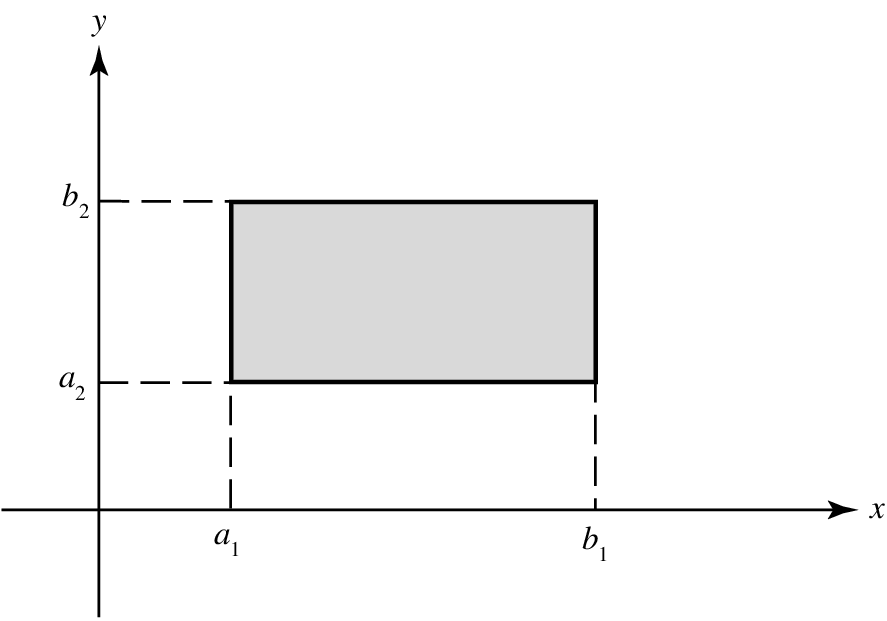
\includegraphics[width=3in,height=2.1in]{png/fig070101.png}
\end{center}
 \vskip6pt
 \refstepcounter{figure}
 \centerline{\bf Figure \thefigure} \label{figure:7.1.1}
 \vskip6pt

The Cartesian product of three
closed intervals
$$
[a_1,b_1]\times [a_2,b_2]\times [a_3,b_3]=\set{(x,y,z)}{a_1\le
x\le b_1,\  a_2\le y\le b_2,\ a_3\le z\le b_3}
$$
is a rectangular parallelepiped in $\R^3$ with faces parallel to the
coordinate axes (Figure~\ref{figure:7.1.2}).




 \vspace*{6pt}
\begin{center}
\includegraphics[width=3.1in,height=2.4in]{png/fig070102.png}
\end{center}
 \vskip6pt
 \refstepcounter{figure}
 \centerline{\bf Figure \thefigure} \label{figure:7.1.2}
 \vskip6pt

\newpage
\begin{definition}\label{thmtype:7.1.1}
A {\it coordinate rectangle\/} $R$ in $\R^n$ is the Cartesian
product of $n$ closed intervals; that is,
$$
R=[a_1,b_1]\times [a_2,b_2]\times\cdots\times [a_n,b_n].
$$
The {\it content\/} of $R$ is
$$
V(R)=(b_1-a_1)(b_2-a_2)\cdots (b_n-a_n).
$$
The numbers $b_1-a_1$, $b_2-a_2$, \dots, $b_n-a_n$ are  the {\it edge
lengths\/} of $R$. If
they are equal, then
$R$ is a
{\it coordinate cube\/}.
 If $a_r=b_r$ for some $r$, then $V(R)=0$ and we
say that $R$ is {\it degenerate\/};
otherwise,
$R$ is
{\it nondegenerate\/}.
 \bbox\end{definition}

If $n=1$, $2$, or $3$, then $V(R)$ is, respectively, the length of an
interval, the area of a rectangle, or the volume of a rectangular
parallelepiped. Henceforth, ``rectangle'' or ``cube'' will always mean
``coordinate rectangle'' or ``coordinate cube'' unless it is stated
otherwise.

If
$$
R=[a_1,b_1]\times [a_2,b_2]\times\cdots\times [a_n,b_n]
$$
and
$$
P_r\colon\, a_r=a_{r0}<a_{r1}<\cdots<a_{rm_r}=b_r\quad
$$
is a partition of  $[a_r,b_r]$,  $1\le r\le n$, then
the set of all rectangles in $\R^n$ that can be written as
$$
[a_{1,j_1-1},a_{1j_1}]\times[a_{2,j_2-1},a_{2j_2}]\times\cdots\times
[a_{n,j_n-1},a_{nj_n}],\quad\
1\le j_r\le m_r,\quad 1\le r\le n,
$$
is  a {\it partition\/} of $R$.
We denote this partition  by
\begin{equation}\label{eq:7.1.1}
{\bf P}=P_1\times P_2\times\cdots\times P_n
\end{equation}
and define its {\it norm\/}
 to be the maximum of the norms of
$P_1$, $P_2$, \dots, $P_n$, as defined in  Section~3.1; thus,
$$
\|{\bf P}\|=\max\{\|P_1\|,\,\|P_2\|, \dots,\|P_n\|\}.
$$
Put another way, $\|{\bf P}\|$ is the largest of the edge lengths of
all the subrectangles in~${\bf P}$.


Geometrically, a rectangle in $\R^2$ is partitioned by drawing
horizontal and vertical lines through it
 (Figure~\ref{figure:7.1.3}); in
$\R^3$, by drawing planes through it parallel to the coordinate
axes. Partitioning divides a rectangle $R$ into finitely many
subrectangles that we can number in arbitrary order as
$R_1$, $R_2$, \dots, $R_k$. Sometimes it is convenient to write
$$
{\bf P}=\{R_1,R_2, \dots,R_k\}
$$
\nopagebreak
rather than \eqref{eq:7.1.1}.
\pagebreak


\topfig{-3}
\begin{center}
\includegraphics[width=3.1in,height=2.35in]{png/fig070103.png}
\end{center}
 \vskip6pt
 \refstepcounter{figure}
 \centerline{\bf Figure \thefigure} \label{figure:7.1.3}
 \vskip12pt

If ${\bf P}=P_1\times P_2\times\cdots\times P_n$ and ${\bf P}'=P'_1
\times P'_2\times\cdots\times P'_n$ are partitions of the same
rectangle, then ${\bf P}'$ is a {\it refinement\/}
 of ${\bf P}$ if
$P'_i$ is a refinement of $P_i$, $1\le i\le n$, as defined
in Section~3.1.

Suppose that $f$ is a real-valued function defined on a rectangle $R$
in $\R^n$, ${\bf P}=\{R_1,R_2, \dots,R_k\}$ is a partition of
$R$, and $\mathbf{X}_j$ is an arbitrary point in $R_j$, $1\le j\le k$.
Then
$$
\sigma=\sum_{j=1}^k f(\mathbf{X}_j)V(R_j)
$$
is a {\it Riemann sum of $f$ over ${\bf P\/}$\/}.
Since $\mathbf{X}_j$
can be chosen arbitrarily in $R_j$, there are infinitely many Riemann
sums for a given function $f$ over any partition ${\bf P}$ of $R$.

The following definition is similar to
Definition~\ref{thmtype:3.1.1}.



\begin{definition}\label{thmtype:7.1.2}
Let $f$ be a real-valued function defined
on a  rectangle $R$ in $\R^n$. We say that
 $f$ is {\it Riemann integrable on\/} $R$
 if there is a number $L$ with the following property: For
every $\epsilon>0$, there is a $\delta>0$ such that
$$
\left|\sigma-L\right|<\epsilon
$$
if $\sigma$ is any Riemann sum of $f$ over
a partition ${\bf P}$ of $R$
such that $\|{\bf P}\|<\delta$.
In this case, we say that
 $L$ is the  {\it Riemann integral of $f$ over\/} $R$, and write
$$
\int_R f(\mathbf{X})\,d\mathbf{X}=L.
\eqno{\bbox}
$$
\end{definition}

If $R$ is degenerate, then Definition~\ref{thmtype:7.1.2} implies that
$\int_R f(\mathbf{X})\,d\mathbf{X}=0$ for any function $f$ defined on $R$
(Exercise~\ref{exer:7.1.1}). Therefore, it should be understood
henceforth
that whenever we speak of a rectangle in $\R^n$ we  mean
a nondegenerate rectangle, unless it is stated to the
contrary.

The integral $\int_R\, f(\mathbf{X})d\mathbf{X}$ is also written as
$$
\int_R f(x,y)\, d(x,y)\quad  (n=2), \quad
\int_R f(x,y,z) \,d(x,y,z)\quad  (n=3),
$$
or
$$
\int_R f(x_1,x_2, \dots,x_n) \,d(x_1,x_2, \dots,x_n) \mbox{\quad($n$
arbitrary)}.
$$

Here $d\mathbf{X}$ does not stand for the differential of $\mathbf{X}$, as
defined in Section~6.2. It merely identifies
$x_1$, $x_2$, \dots, $x_n$, the components of $\mathbf{X}$, as the
variables
of integration. To avoid this minor inconsistency, some authors write
simply $\int_R f$ rather than $\int_R f(\mathbf{X})\, d\mathbf{X}$.

As in the case where $n=1$, we will say simply ``integrable'' or
``integral'' when we mean ``Riemann integrable'' or ``Riemann
integral.'' If $n\ge2$, we call the integral of
Definition~\ref{thmtype:7.1.2} a {\it multiple integral\/};
 for $n=2$ and
$n=3$ we also call them {\it double\/}
 and {\it triple integrals\/},
respectively. When we wish to distinguish between multiple integrals
and the integral we studied in Chapter~\ $(n=1)$, we will
call the latter an {\it ordinary\/} integral.

\begin{example}\label{example:7.1.1}\rm
Find $\int_Rf(x,y)\,d(x,y)$,
where
$$
R=[a,b]\times [c,d]
$$
and
$$
f(x,y)=x+y.
$$
\end{example}

\solution
Let $P_1$ and $P_2$ be partitions of $[a,b]$ and $[c,d]$; thus,
$$
P_1: a=x_0<x_1<\cdots<x_r=b
\mbox{\quad and \quad}
P_2: c=y_0<y_1<\cdots<y_s=d.
$$
A typical Riemann sum of $f$ over ${\bf P}=P_1\times P_2$ is given by
\begin{equation}\label{eq:7.1.2}
\sigma=\sum_{i=1}^r\sum_{j=1}^s (\xi_{ij}+\eta_{ij})(x_i-x_{i-1})
(y_j-y_{j-1}),
\end{equation}
where
\begin{equation}\label{eq:7.1.3}
x_{i-1}\le\xi_{ij}\le x_i\mbox{\quad and\quad} y_{j-1}\le\eta_{ij}
\le y_j.
\end{equation}
The midpoints of $[x_{i-1}, x_i]$ and $[y_{j-1}, y_j]$ are
\begin{equation}\label{eq:7.1.4}
\overline{x}_i=\frac{x_i+x_{i-1}}{2}\mbox{\quad and\quad}
\overline{y}_j=\frac{y_j+y_{j-1}}{2},
\end{equation}
and \eqref{eq:7.1.3} implies that
\begin{eqnarray}
|\xi_{ij}-\overline{x}_i|\ar\le\frac{x_i-x_{i-1}}{2}\le
\frac{\|P_1\|}{
2}\le \frac{\|{\bf P}\|}{2}\label{eq:7.1.5}\\
\arraytext{and}\nonumber\\
|\eta_{ij}-\overline{y}_j|\ar\le\frac{y_j-y_{j-1}}{2}\le
\frac{\|P_2\|}{2}
\le \frac{\|{\bf P}\|}{2}. \label{eq:7.1.6}
\end{eqnarray}
\newpage
\noindent
Now we rewrite \eqref{eq:7.1.2} as
\begin{equation}\label{eq:7.1.7}
\begin{array}{rcl}
\sigma\ar=\dst{\sum_{i=1}^r\sum_{j=1}^s (\overline{x}_i+
\overline{y}_j)(x_i-x_{i-1}) (y_j-y_{j-1})}\\[2\jot]
\ar{}+\dst{\sum_{i=1}^r\sum_{j=1}^s\left[(\xi_{ij}-\overline{x}_i)+
(\eta_{ij}-\overline{y}_j)\right] (x_i-x_{i-1})(y_j-y_{j-1})}.
\end{array}
\end{equation}
To find $\int_R f(x,y) \,d(x,y)$ from \eqref{eq:7.1.7}, we recall that
\begin{equation}\label{eq:7.1.8}
\sum_{i=1}^r (x_i-x_{i-1})=b-a,\quad\sum_{j=1}^s (y_j-y_{j-1})=d-c
\end{equation}
(Example~\ref{example:3.1.1}), and
\begin{equation}\label{eq:7.1.9}
\sum_{i=1}^r (x^2_i-x^2_{i-1})=b^2-a^2,\quad\sum_{j=1}^s (y_j^2-
y_{j-1}^2)=d^2-c^2
\end{equation}
(Example~\ref{example:3.1.2}).

Because of \eqref{eq:7.1.5} and \eqref{eq:7.1.6} the absolute value of the
second sum in \eqref{eq:7.1.7} does not exceed
\begin{eqnarray*}
\|{\bf P}\|\sum_{j=1}^r\sum_{j=1}^s (x_i-x_{i-1})(y_j-y_{j-1})\ar=
\|{\bf P}\|
\left[\sum_{i=1}^r(x_i-x_{i-1})\right]\left[\sum_{j=1}^s(y_j-y_{j-1})
\right]\\
\ar=\|{\bf P}\| (b-a)(d-c)
\end{eqnarray*}
(see \eqref{eq:7.1.8}), so \eqref{eq:7.1.7} implies that
\begin{equation}\label{eq:7.1.10}
\left|\sigma-\sum_{i=1}^r\sum_{j=1}^s (\overline{x}_i+
\overline{y}_j)(x_i-x_{i-1})(y_j-y_{j-1})\right|\le\|{\bf P}\|(b-a)(d-c).
\end{equation}
\nopagebreak
It now follows that
$$
\begin{array}{rcl}
\dst{\sum_{i=1}^r}\dst{\sum_{j=1}^s}\,\overline{x}_i(x_i-x_{i-1})(y_j-y_{j-1})
\ar=\dst{\left[\sum_{i=1}^r\overline{x}_i(x_i-x_{i-1})\right]}
\dst{\left[\sum_{j=1}^s(y_j-y_{j-1})\right]}\\
\ar=(d-c)\dst{\sum_{i=1}^r}\overline{x}_i(x_i-x_{i-1})\mbox{\quad(from
\eqref{eq:7.1.8})}\\
\ar=\dst\frac{d-c}{2}\sum_{i=1}^r
(x^2_i-x^2_{i-1})\hspace*{2.1em}\mbox{(from
\eqref{eq:7.1.4})}\\
\ar=\dst\frac{d-c}{2}(b^2-a^2)\hspace*{4.6em}\mbox{(from
\eqref{eq:7.1.9})}.
\end{array}
$$
Similarly,
$$
\sum_{i=1}^r\sum_{j=1}^s\overline{y}_j(x_i-x_{i-1}) (y_j-y_{j-1})=
\frac{b-a}{2}(d^2-c^2).
$$
\newpage
\noindent
Therefore, \eqref{eq:7.1.10} can be written as
$$
\left|\sigma-\frac{d-c}{2}(b^2-a^2)-\frac{b-a}{2}(d^2-c^2)\right|\le
\|{\bf P}\|(b-a)(d-c).
$$
Since the right side can be made as small as we wish by choosing
$\|{\bf P}\|$ sufficiently small,
$$
\int_R (x+y) \,d(x,y)=\frac{1}{2}\left[(d-c)(b^2-a^2)+(b-a)(d^2-c^2)\right].
$$

\boxit{Upper and Lower Integrals}
The following theorem is analogous to
Theorem~\ref{thmtype:3.1.2}.

\begin{theorem}\label{thmtype:7.1.3}
If $f$ is unbounded on the nondegenerate rectangle $R$ in
$\R^n,$ then $f$ is not integrable on $R.$
\end{theorem}


\proof
 We will show that if $f$ is unbounded on $R$, ${\bf
P}=\{R_1,R_2, \dots,R_k\}$ is
any partition of $R$, and $M>0$, then there are Riemann sums $\sigma$
and $\sigma'$ of $f$ over ${\bf P}$ such that
\begin{equation} \label{eq:7.1.11}
|\sigma-\sigma'|\ge M.
\end{equation}
This implies  that
$f$ cannot satisfy Definition~\ref{thmtype:7.1.2}. (Why?)

Let
$$
\sigma=\sum_{j=1}^kf(\mathbf{X}_j)V(R_j)
$$
be a Riemann sum of $f$ over  ${\bf P}$. There must be
an integer $i$ in $\{1,2, \dots,k\}$ such that
\begin{equation} \label{eq:7.1.12}
|f(\mathbf{X})-f(\mathbf{X}_i)|\ge\frac{M }{ V(R_i)}
\end{equation}
for some $\mathbf{X}$ in $R_i$, because if this were not so, we
would have
$$
|f(\mathbf{X})-f(\mathbf{X}_j)|<\frac{M}{ V(R_j)},\quad \mathbf{X}\in R_j,\quad
\quad 1\le j\le k.
$$
If this is so, then
\begin{eqnarray*}
|f(\mathbf{X})|\ar=|f(\mathbf{X}_j)+f(\mathbf{X})-f(\mathbf{X}_j)|\le|f(\mathbf{X}_j)|+|f(\mathbf{X})-f(\mathbf{X}_j)|\\
\ar\le |f(\mathbf{X}_j)|+\frac{M}{ V(R_j)},\quad \mathbf{X}\in R_j,\quad
1\le j\le k.
\end{eqnarray*}
However, this implies that
$$
|f(\mathbf{X})|\le\max\set{|f(\mathbf{X}_j)|+\frac{M}{ V(R_j)}}{1\le j\le k},
\quad \mathbf{X}\in R,
$$
which contradicts the assumption that $f$ is unbounded on $R$.

 Now  suppose that $\mathbf{X}$ satisfies \eqref{eq:7.1.12}, and
consider the Riemann sum
$$
\sigma'=\sum_{j=1}^nf(\mathbf{X}_j')V(R_j)
$$
over the same partition ${\bf P}$, where
$$
\mathbf{X}_j'=\left\{\casespace\begin{array}{ll}
\mathbf{X}_j,&j \ne i,\\
\mathbf{X},&j=i.\end{array}\right.
$$
Since
$$
|\sigma-\sigma'|=|f(\mathbf{X})-f(\mathbf{X}_i)|V(R_i),
$$
\eqref{eq:7.1.12} implies \eqref{eq:7.1.11}.
\bbox

Because of Theorem~\ref{thmtype:7.1.3}, we need consider only bounded
functions in connection with Definition~\ref{thmtype:7.1.2}. As in the
case where $n=1$, it is now convenient to define the upper and lower
integrals of a bounded function over a rectangle.  The following
definition is   analogous to Definition~\ref{thmtype:3.1.3}.


\begin{definition} \label{thmtype:7.1.4}
If $f$ is bounded on a rectangle $R$ in $\R^n$ and
${\bf P}=\{R_1,R_2, \dots,R_k\}$ is a partition of $R$, let
$$
M_j=\sup_{\mathbf{X}\in R_j}f(\mathbf{X}),\quad m_j=
\inf_{\mathbf{X}\in R_j}f(\mathbf{X}).
$$
The {\it upper sum\/} of $f$ over ${\bf P}$ is
$$
S({\bf P})=\sum_{j=1}^k M_jV(R_j),
$$
and the {\it upper integral
 of $f$ over\/} $R$, denoted by
$$
\overline{\int_R}\,f(\mathbf{X})\,d\mathbf{X},
$$
 is the infimum of all  upper
sums. The {\it lower sum of $f$ over\/} ${\bf P}$ is
$$
s({\bf P})=\sum_{j=1}^k m_jV(R_j),
$$
and the {\it lower integral
 of $f$ over \/}$R$, denoted by
$$
\underline{\int_R}\, f(\mathbf{X})\,d\mathbf{X},
$$
 is the supremum of all  lower sums.
\bbox\end{definition}


The following theorem is analogous to
Theorem~\ref{thmtype:3.1.4}.

\begin{theorem}  \label{thmtype:7.1.5}
Let $f$ be bounded on a rectangle  $R$  and let $\mathbf{P}$
be a partition of $R.$  Then
\begin{alist}
\item % (a)
 The upper sum $S(\mathbf{P})$ of $f$ over $\mathbf{P}$ is the supremum
of the set of all Riemann sums of $f$ over $\mathbf{P}.$
\item % (b)
 The lower sum $s(\mathbf{P})$ of $f$ over $\mathbf{P}$ is the infimum
 of the set of all Riemann sums of $f$ over $\mathbf{P}.$
\end{alist}
\end{theorem}

\proof Exercise~\ref{exer:7.1.5}.





If
$$
m\le f(\mathbf{X})\le M\mbox{\quad for $\mathbf{X}$ in $R$},
$$
then
$$
mV(R)\le s({\bf P})\le S({\bf P})\le MV(R);
$$
therefore, $\overline{\int_R}\, f(\mathbf{X})\,d\mathbf{X}$ and
$\underline{\int_R}\, f(\mathbf{X})\, d\mathbf{X}$ exist, are unique, and
satisfy the inequalities
$$
mV(R)\le\overline{\int_R}\, f(\mathbf{X})\,d\mathbf{X}\le MV(R)
$$
and
$$
mV(R)\le\underline{\int_R}\, f(\mathbf{X})\,d\mathbf{X}\le MV(R).
$$

The upper and lower integrals are also written as
$$
\overline{\int_R}\, f(x,y) \,d(x,y)\mbox{\quad and\quad}\underline{\int_R}\,
f(x,y) \,d(x,y)\quad (n=2),
$$
$$
\overline{\int_R}\, f(x,y,z) \,d(x,y,z)\mbox{\quad and\quad}
\underline{\int_R}\, f(x,y,z) \,d(x,y,z)\quad (n=3),
$$
or
$$
\overline{\int_R}\, f(x_1,x_2, \dots,x_n) \,d(x_1,x_2, \dots,x_n)
$$
and
$$
\underline{\int_R}\, f(x_1,x_2, \dots,x_n)\,d(x_1,x_2, \dots,x_n)\quad
\mbox{\quad ($n$ arbitrary)}.
$$

\begin{example}\label{example:7.1.2}\rm
Find $\underline{\int_R}\,f(x,y)\,d(x,y)$ and
 $\overline{\int_R}\,f(x,y)\,d(x,y)$, with
$R=[a,b]\times [c,d]$ and
$$
f(x,y)=x+y,
$$
as in Example~\ref{example:7.1.1}.
\bbox\end{example}

\solution
Let $P_1$ and $P_2$ be partitions of $[a,b]$ and $[c,d]$; thus,
$$
P_1: a=x_0<x_1<\cdots<x_r=b\mbox{\quad and \quad}
P_2: c=y_0<y_1<\cdots<y_s=d.
$$
\newpage
\noindent
The maximum and minimum values of $f$ on the rectangle $[x_{i-1},
x_i] \times [y_{j-1},y_j]$ are $x_i+y_j$ and $x_{i-1}+y_{j-1}$,
respectively. Therefore,
\begin{eqnarray}
S({\bf P})\ar=\sum_{i=1}^r\sum_{j=1}^s (x_i+y_j)(x_i-x_{i-1})
(y_j-y_{j-1})  \label{eq:7.1.13}\\
\arraytext{and}\nonumber\\
s({\bf P})\ar=\sum_{i=1}^r\sum_{j=1}^s (x_{i-1}+y_{j-1}) (x_i-x_{i-1})
(y_j-y_{j-1}). \label{eq:7.1.14}
\end{eqnarray}
By substituting
$$
x_i+y_j=\frac{1}{2}[(x_i+x_{i-1})+(y_j+y_{j-1})+
(x_i-x_{i-1})+(y_j-y_{j-1})]
$$
into \eqref{eq:7.1.13}, we find that
\begin{equation}\label{eq:7.1.15}
S({\bf P})=\frac{1}{2}(\Sigma_1+\Sigma_2+\Sigma_3+\Sigma_4),
\end{equation}
where
$$
\begin{array}{rclcl}
\Sigma_1\ar=\dst{\sum_{i=1}^r(x_i^2-x_{i-1}^2)
\sum_{j=1}^s(y_j-y_{j-1})}\ar=(b^2-a^2)(d-c),\\[2\jot]
\Sigma_2\ar=\dst{\sum_{i=1}^r(x_i-x_{i-1})
\sum_{j=1}^s(y_j^2-y_{j-1}^2)}\ar=(b-a)(d^2-c^2),\\[2\jot]
\Sigma_3\ar=\dst{\sum_{i=1}^r(x_i-x_{i-1})^2
\sum_{j=1}^s(y_j-y_{j-1})}\ar\le \|\mathbf{P}\|(b-a)(d-c),\\[2\jot]
\Sigma_4\ar=\dst{\sum_{i=1}^r(x_i-x_{i-1})
\sum_{j=1}^s(y_j-y_{j-1})^2}\ar\le \|\mathbf{P}\|(b-a)(d-c).
\end{array}
$$
Substituting these four results into \eqref{eq:7.1.15} shows that
$$
I<S({\bf P})<I+\|{\bf P}\|(b-a)(d-c),
$$
where
$$
I=\frac{(d-c)(b^2-a^2)+(b-a)(d^2-c^2)}{2}.
$$
From this, we see that
$$
\overline{\int_R}\,(x+y) \,d(x,y)=I.
$$


After substituting
$$
x_{i-1}+y_{j-1}=\frac{1}{2}[(x_i+x_{i-1})+(y_j+y_{j-1})-(x_i-x_{i-1})
-(y_j-y_{j-1})]
$$
into \eqref{eq:7.1.14}, a similar argument shows that
$$
I-\|{\bf P}\|(b-a)(d-c)<s({\bf P})<I,
$$
\newpage
\noindent
so
$$
\underline{\int_R}\, (x+y)\,d(x,y)=I.
\eqno{\bbox}
$$

We now prove an analog of Lemma~\ref{thmtype:3.2.1}.

\begin{lemma}\label{thmtype:7.1.6}
Suppose that $|f(\mathbf{X})|\le
M$ if $\mathbf{X}$ is in the rectangle
$$
R=[a_1,b_1]\times [a_2,b_2]\times\cdots\times [a_n,b_n].
$$
Let ${\bf P}=P_1\times P_2\times\cdots\times P_n$ and ${\bf P}'=
P_1'\times P_2'\times\cdots\times P_n'$ be partitions of $R,$ where
$P_j'$ is obtained by adding $r_j$ partition points to $P_j,$
$1\le j\le n.$ Then
\begin{equation}\label{eq:7.1.16}
S({\bf P})\ge S({\bf P}')\ge S({\bf P})-2MV(R)\left(\sum_{j=1}^n
\frac{r_j}{ b_j-a_j}\right)\|{\bf P}\|
\end{equation}
and
\begin{equation}\label{eq:7.1.17}
s({\bf P})\le s({\bf P}')\le s({\bf P})+2MV(R)\left(\sum_{j=1}^n
\frac{r_j
}{ b_j-a_j}\right)\|{\bf P}\|.
\end{equation}
\end{lemma}

\proof
We will prove
 \eqref{eq:7.1.16} and leave the proof of \eqref{eq:7.1.17} to you
(Exercise~\ref{exer:7.1.7}).
First suppose that
 $P_1'$ is obtained by adding one point to $P_1$, and
$P_j'=P_j$ for $2\le j\le n$.
If $P_r$ is
defined by
$$
P_r: a_r=a_{r0}<a_{r1}<\cdots<a_{rm_r}=b_r,\quad 1\le r\le n,
$$
then a typical subrectangle of ${\bf P}$ is of the form
$$
R_{j_1j_2\cdots j_n}=[a_{1,j_1-1}, a_{1j_1}]\times
[a_{2,j_2-1},a_{2j_2}]\times\cdots\times [a_{n,j_n-1}, a_{nj_n}].
$$
Let $c$ be the additional point introduced into $P_1$ to obtain
$P_1'$, and suppose that
$$
a_{1,k-1}<c<a_{1k}.
$$
If $j_1\ne k$, then $R_{j_1j_2\cdots j_n}$
 is common
to ${\bf P}$ and ${\bf P}'$, so the terms associated with it in
$S({\bf P}')$
and $S({\bf P})$ cancel in the difference $S({\bf P})-S({\bf P}')$.  To
analyze the terms that do not cancel, define
$$
\begin{array}{rcl}
R^{(1)}_{kj_2\cdots j_n}\ar=[a_{1,k-1}, c]\times [a_{2,j_2-1},
a_{2j_2}]
\times\cdots\times [a_{n,j_n-1},a_{nj_n}],\\[2\jot]
R^{(2)}_{kj_2\cdots j_n}\ar=[c,a_{1k}]\times [a_{2,j_2-1}, a_{2j_2}]
\times\cdots\times [a_{n,j_n-1}, a_{nj_n}],
\end{array}
$$
\begin{equation} \label{eq:7.1.18}
M_{kj_2\cdots j_n}=\sup\set{f(\mathbf{X})}{\mathbf{X}\in
R_{kj_2\cdots j_n}}
\end{equation}
and
\begin{equation} \label{eq:7.1.19}
\begin{array}{rcl}
M^{(i)}_{kj_2\cdots j_n}=\sup\set{f(\mathbf{X})}{\mathbf{X}
\in R^{(i)}_{kj_2\cdots j_n}},\quad i=1,2.
\end{array}
\end{equation}

\newpage
\noindent
Then $S({\bf P})-S({\bf P}')$ is the sum of terms of the form
\begin{equation}\label{eq:7.1.20}
\begin{array}{c}
\left[M_{kj_2\cdots
j_n}(a_{1k}-a_{1,k-1})-M^{(1)}_{kj_2
\cdots j_n} (c-a_{1,k-1})-M^{(2)}_{kj_2\cdots
j_n}(a_{1k}-c)\right]\\
\times (a_{2j_2}-a_{2,j_2-1})\cdots (a_{nj_n}-a_{n,j_n-1}).
\end{array}
\end{equation}
\noindent The terms within the brackets can be rewritten as
\begin{equation}\label{eq:7.1.21}
(M_{kj_2\cdots j_n}-M^{(1)}_{kj_2\cdots
j_n})(c-a_{1,k-1})+(M_{kj_2\cdots
j_n}-M^{(2)}_{kj_2\cdots j_n})(a_{1k}-c),
\end{equation}
\noindent
which is nonnegative, because of \eqref{eq:7.1.18} and \eqref{eq:7.1.19}.
Therefore,
\begin{equation}\label{eq:7.1.22}
S({\bf P}')\le S({\bf P}).
\end{equation}
Moreover, the quantity in \eqref{eq:7.1.21} is not greater than
$2M(a_{1k}-a_{1,k-1})$, so \eqref{eq:7.1.20} implies that the general
surviving term in $S({\bf P})-S({\bf P}')$ is not greater than
$$
2M\|{\bf P}\|(a_{2j_2}-a_{2,j_2-1})\cdots (a_{nj_n}-a_{n,j_n-1}).
$$
The sum of these terms as $j_2$, \dots, $j_n$ assume all possible
values
$1 \le j_i\le m_i$, $2\le i\le n$, is
$$
2M\|{\bf P}\|(b_2-a_2)\cdots (b_n-a_n)=\frac{2M\|{\bf P}\|V(R)}{ b_1-a_1}.
$$
This implies that
$$
S({\bf P})\le S({\bf P}')+\frac{2M\|{\bf P}\|V(R)}{ b_1-a_1}.
$$
This and \eqref{eq:7.1.22} imply \eqref{eq:7.1.16} for $r_1=1$ and
$r_2=\cdots=r_n=0$.

Similarly, if $r_i=1$ for some $i$ in $\{1, \dots,n\}$
and $r_j=0$ if $j\ne i$, then
$$
S({\bf P})\le S({\bf P}')+\frac{2M\|{\bf P}\|V(R)}{ b_i-a_i}.
$$
To obtain \eqref{eq:7.1.16} in the general case,
 repeat this argument $r_1+r_2+\cdots+r_n$ times, as in
the proof of Lemma~\ref{thmtype:3.2.1}.
\bbox


Lemma~\ref{thmtype:7.1.6} implies the following theorems and lemma, with
proofs analogous to the proofs of their counterparts in
Section~3.2.


\begin{theorem}\label{thmtype:7.1.7}
If $f$ is bounded on a rectangle $R,$ then
$$
\underline{\int_R}\, f(\mathbf{X})\,d\mathbf{X}
\le\overline{\int_R}\, f(\mathbf{X})\,d\mathbf{X}.
$$
\end{theorem}



\proof  Exercise~\ref{exer:7.1.8}.

The next theorem is analogous to Theorem~3.2.3.

\begin{theorem}\label{thmtype:7.1.8}
If $f$ is integrable on a rectangle $R,$ then
$$
\underline{\int_R}\, f(\mathbf{X})\,d\mathbf{X}=
\overline{\int_R}\, f(\mathbf{X})\,d\mathbf{X} =\int_R f(\mathbf{X})\,d\mathbf{X}.
$$
\end{theorem}

\nopagebreak
\proof  Exercise~\ref{exer:7.1.9}.
\newpage


\enlargethispage{\baselineskip}
\begin{lemma}\label{thmtype:7.1.9}
If $f$ is bounded on a rectangle $R$ and $\epsilon>0,$  there is
 a $\delta>0$ such that
\vspace{4pt}
$$
\overline{\int_R}\, f(\mathbf{X})\,d\mathbf{X}\le S({\bf P})<\overline{\int_R}\,
f(\mathbf{X})\,d\mathbf{X}+\epsilon
$$
\vspace{4pt}
and
\vspace{4pt}
$$
\underline{\int_R}\, f(\mathbf{X})\,d\mathbf{X}\ge s({\bf P})>
\underline{\int_R}\, f(\mathbf{X})\,d\mathbf{X}-\epsilon
$$
\vspace{4pt}
if $\|{\bf P}\|<\delta.$
\end{lemma}



\proof Exercise~\ref{exer:7.1.10}.


The next theorem is analogous to Theorem~3.2.5.

\begin{theorem}\label{thmtype:7.1.10}
If $f$ is bounded on a rectangle $R$ and
\vspace{2pt}
$$
\underline{\int_R}\, f(\mathbf{X})\,d\mathbf{X}=
\overline{\int_R}\, f(\mathbf{X})\,d\mathbf{X}=L,
$$
\vspace{2pt}
then $f$ is integrable on $R,$ and
\vspace{2pt}
$$
\int_R f(\mathbf{X})\,d\mathbf{X}=L.
$$
\end{theorem}

\proof  Exercise~\ref{exer:7.1.11}.


Theorems~\ref{thmtype:7.1.8} and \ref{thmtype:7.1.10}
 imply the following theorem, which is analogous to
Theorem~\ref{thmtype:3.2.6}.

\begin{theorem} \label{thmtype:7.1.11}
A bounded
function $f$ is integrable on a rectangle $R$ if and only if
$$
\underline{\int_R}\, f(\mathbf{X})\,d\mathbf{X}=\overline{\int_R}\, f(\mathbf{X})\,
d\mathbf{X}.
$$
\end{theorem}

The next theorem translates this into a test that can be
conveniently applied.
It is analogous to
Theorem~\ref{thmtype:3.2.7}.

\begin{theorem}\label{thmtype:7.1.12}
If $f$ is bounded on a rectangle $R,$ then $f$ is integrable on $R$
if and only if for every $\epsilon>0$ there is a partition ${\bf P}$
of $R$ such that
$$
S({\bf P})-s({\bf P})<\epsilon.
$$
\end{theorem}

\proof  Exercise~\ref{exer:7.1.12}.

Theorem~\ref{thmtype:7.1.12} provides a useful criterion for
integrability. The next theorem is an important application.
It is analogous to
Theorem~\ref{thmtype:3.2.8}.


\begin{theorem}\label{thmtype:7.1.13}
If $f$ is continuous on a rectangle $R$ in $\R^n,$ then $f$ is
integrable on~$R.$
\end{theorem}

\newpage


\proof
Let $\epsilon>0$. Since $f$ is uniformly continuous on $R$
(Theorem~\ref{thmtype:5.2.14}), there is a $\delta>0$ such that
\begin{equation} \label{eq:7.1.23}
|f(\mathbf{X})-f(\mathbf{X}')|<\frac{\epsilon}{ V({\bf R})}
\end{equation}
if $\mathbf{X}$ and $\mathbf{X}'$ are in $R$ and
 $|\mathbf{X}-\mathbf{X}'|<\delta$. Let ${\bf P}=\{R_1,R_2, \dots,R_k\}$ be a partition of
$R$ with $\|P\|<\delta/\sqrt n$. Since $f$ is continuous on $R$, there
are points $\mathbf{X}_j$ and $\mathbf{X}_j'$ in $R_j$ such that
$$
f(\mathbf{X}_j)=M_j=\sup_{\mathbf{X}\in R_j}f(\mathbf{X})
\mbox{\quad and \quad}
f(\mathbf{X}_j')=m_j=\inf_{\mathbf{X}\in R_j}f(\mathbf{X})
$$
(Theorem~\ref{thmtype:5.2.12}).
Therefore,
$$
S(\mathbf{P})-s(\mathbf{P})=\sum_{j=1}^n(f(\mathbf{X}_j)-
f(\mathbf{X}_j'))V(R_j).
$$
Since $\|{\bf P}\|<\delta/\sqrt n$,
$|\mathbf{X}_j-\mathbf{X}_j'|<\delta$, and, from \eqref{eq:7.1.23}
with $\mathbf{X}=\mathbf{X}_j$ and $\mathbf{X}'=\mathbf{X}_j'$,
$$
 S(\mathbf{P})-s(\mathbf{P})<\frac{\epsilon}{ V(R)}
\sum_{j=1}^kV(R_j)=\epsilon.
$$
Hence, $f$ is integrable
on $R$, by Theorem~\ref{thmtype:7.1.12}.



\boxit{Sets with Zero Content}
The next definition will enable us to establish  the existence
of $\int_Rf(\mathbf{X})\,d\mathbf{X}$ in cases where $f$ is bounded on the
rectangle $R$, but is not necessarily continuous for all $\mathbf{X}$
in $R$.



\begin{definition}\label{thmtype:7.1.14}
A subset $E$ of $\R^n$ has zero content if for each
$\epsilon>0$
there is a finite set of rectangles $T_1$, $T_2$, \dots, $T_m$ such
that
\begin{equation}\label{eq:7.1.24}
E\subset\bigcup_{j=1}^m T_j
\end{equation}
and
\begin{equation}\label{eq:7.1.25}
\sum_{j=1}^m V(T_j)<\epsilon.
\end{equation}
\end{definition}



\begin{example}\label{example:7.1.3}\rm Since the empty set is contained
in every rectangle, the empty set has zero content. If $E$ consists of
finitely
many points $\mathbf{X}_1$, $\mathbf{X}_2$, \dots,
$\mathbf{X}_m$, then $\mathbf{X}_j$ can be enclosed in a rectangle $T_j$
such that
$$
V(T_j)<\frac{\epsilon}{ m},\quad 1\le j\le m.
$$
Then \eqref{eq:7.1.24} and \eqref{eq:7.1.25} hold,  so $E$ has zero content.
\end{example}


\begin{example}\label{example:7.1.4}\rm Any bounded set $E$ with only
finitely many limit points has zero content. To see this, we first
observe that if $E$ has no limit points, then it must be finite, by
the Bolzano--Weierstrass theorem (Theorem~\ref{thmtype:1.3.8}), and
therefore must have zero content,
by Example~\ref{example:7.1.3}. Now suppose that the limit points of  $E$ are
$\mathbf{X}_1$, $\mathbf{X}_2$, \dots, $\mathbf{X}_m$. Let $R_1$, $R_2$,
\dots, $R_m$ be rectangles such that
$\mathbf{X}_i\in R^0_i$ and
\begin{equation}\label{eq:7.1.26}
V(R_i)<\frac{\epsilon}{2m},\quad 1\le i\le m.
\end{equation}
The set of points of $E$ that are not in $\cup_{j=1}^mR_j$ has no
limit points (why?) and, being bounded, must be finite (again by the
Bolzano--Weierstrass theorem). If this set contains $p$ points,
then it can be covered by rectangles
$R_1'$, $R_2'$, \dots, $R_p'$ with
\begin{equation}\label{eq:7.1.27}
V(R_j')<\frac{\epsilon}{2p},\quad 1\le j\le p.
\end{equation}
Now,
$$
E\subset\left(\bigcup_{i=1}^mR_i\right)\bigcup\left(\bigcup^p_{j=1}
R_j'\right)
$$
and, from \eqref{eq:7.1.26} and \eqref{eq:7.1.27},
$$
\sum_{i=1}^m V(R_i)+\sum_{j=1}^p V(R_j')<\epsilon.
$$
\end{example}



\begin{example}\label{example:7.1.5}\rm
  If $f$ is continuous on $[a,b]$,
then the curve
\begin{equation}\label{eq:7.1.28}
y=f(x),\quad a\le x\le b
\end{equation}
(that is, the set $\set{(x,y)}{y=f(x),\ a\le x\le b})$, has zero
content in $\R^2$. To see this, suppose that $\epsilon>0$, and
choose $\delta>0$ such that
\begin{equation}\label{eq:7.1.29}
|f(x)-f(x')|<\epsilon\mbox{\quad if\quad} x, x'\in [a,b]
\mbox{\quad and\quad} |x-x'|<\delta.
\end{equation}
This is possible because $f$ is uniformly continuous on $[a,b]$
(Theorem~\ref{thmtype:2.2.12}). Let
$$
P: a=x_0<x_1<\cdots<x_n=b
$$
be a partition of $[a,b]$ with $\|P\|<\delta$, and
choose $\xi_1$, $\xi_2$, \dots, $\xi_n$ so that
$$
x_{i-1}\le\xi_i\le x_i,\quad 1\le i\le n.
$$
 Then, from \eqref{eq:7.1.29},
$$
|f(x)-f(\xi_i)|<\epsilon\mbox{\quad if\quad}\ x_{i-1}\le x\le x_i.
$$
This means that every point on the curve \eqref{eq:7.1.28} above the
interval $[x_{i-1},x_i]$ is in a rectangle with area $2\epsilon
(x_i-x_{i-1})$ (Figure~\ref{figure:7.1.4}).
Since the total
area of these rectangles is $2\epsilon (b-a)$,  the curve has zero
content.
\end{example}
\newpage

\enlargethispage{-2\baselineskip}
\topfig{-3}
\begin{center}
\includegraphics[width=4in,height=2.5in]{png/fig070104.png}
\end{center}
 \vskip6pt
 \refstepcounter{figure}
 \centerline{\bf Figure \thefigure} \label{figure:7.1.4}
 \vskip12pt



The next lemma follows immediately from
Definition~\ref{thmtype:7.1.14}.

\begin{lemma}\label{thmtype:7.1.15}
The union of finitely many sets with zero content has zero content$.$
\end{lemma}

The following theorem will enable us to define multiple
integrals over more general subsets of $\R^n$.


\begin{theorem}\label{thmtype:7.1.16}
Suppose that $f$ is bounded on a rectangle
\begin{equation}\label{eq:7.1.30}
R=[a_1,b_1]\times [a_2,b_2]\times\cdots\times [a_n,b_n]
\end{equation}
and continuous except on a subset $E$ of $R$ with zero content$.$ Then
$f$ is integrable on $R.$
\end{theorem}

\proof
 Suppose that $\epsilon>0$. Since $E$ has zero content, there are
rectangles
$T_1$, $T_2$, \dots, $T_m$  such that
\begin{equation} \label{eq:7.1.31}
E\subset\bigcup_{j=1}^m T_j
\end{equation}
and
\begin{equation} \label{eq:7.1.32}
\sum_{j=1}^m V(T_j)<\epsilon.
\end{equation}
 We may assume  that
$T_1$, $T_2$, \dots, $T_m$ are contained in $R$, since, if not, their
intersections with
$R$ would be contained in $R$, and still satisfy \eqref{eq:7.1.31}
and \eqref{eq:7.1.32}.
 We may also assume that if $T$ is any rectangle such
that
\begin{equation}\label{eq:7.1.33}
T\bigcap\left(\bigcup_{j=1}^m T_j^0\right)=\emptyset, \mbox{\quad
then
\quad}T\cap E=\emptyset
\end{equation}
\newpage
\noindent
since if this were not so, we could make it so by  enlarging
$T_1$, $T_2$, \dots, $T_m$
slightly while maintaining \eqref{eq:7.1.32}. Now suppose that
\vspace*{1pt}
$$
T_j=[a_{1j},b_{1j}]\times [a_{2j},b_{2j}]\times\cdots\times
[a_{nj},b_{nj}],\quad 1\le j\le m,
$$
\vspace*{1pt}
\noindent let $P_{i0}$ be the partition of $[a_i,b_i]$ (see
\eqref{eq:7.1.30}) with partition points
$$
a_i,b_i,a_{i1},b_{i1},a_{i2},b_{i2}, \dots,a_{im},b_{im}
\vspace*{1pt}
$$
(these are not in increasing order), $1\le i\le n$, and let
\vspace*{1pt}
$$
{\bf P}_0=P_{10}\times P_{20}\times\cdots\times P_{n0}.
$$
\vspace*{1pt}
\noindent\hskip-.3em Then ${\bf P}_0$ consists of rectangles whose
union equals  $\cup_{j=1}^m T_j$
and other rectangles
$T'_1$, $T'_2$, \dots, $T'_k$ that do not intersect $E$. (We need
\eqref{eq:7.1.33} to be sure that $T'_i\cap E=\emptyset,
1\le i\le k.)$ If we let
$$
B=\bigcup_{j=1}^m T_j\mbox{\quad and\quad} C=\bigcup^k_{i=1} T'_i,
$$
then $R=B\cup C$ and $f$ is continuous on the compact set $C$.
If ${\bf P}=\{R_1,R_2, \dots,R_k\}$ is a refinement of ${\bf P}_0$,
then every subrectangle $R_j$ of ${\bf P}$ is contained entirely in
$B$ or entirely in $C$. Therefore, we can write
\vspace*{1pt}
\begin{equation}\label{eq:7.1.34}
S({\bf P})-s({\bf P})=\Sigma_1(M_j-m_j)
V(R_j)+\Sigma_2(M_j-m_j)V(R_j),
\end{equation}
\vspace*{1pt}
\noindent \hskip-.3em
where $\Sigma_1$ and $\Sigma_2$ are summations over values of $j$ for
which $R_j\subset B$ and $R_j\subset C$, respectively. Now suppose that
$$
|f(\mathbf{X})|\le M\mbox{\quad for $\mathbf{X}$ in $R$}.
$$
Then
\begin{equation}\label{eq:7.1.35}
\Sigma_1(M_j-m_j) V(R_j)\le2M\,\Sigma_1 V(R_j)=2M\sum_{j=1}^m V(T_j)<
2M\epsilon,
\end{equation}
from \eqref{eq:7.1.32}.
Since $f$ is uniformly continuous  on the compact set $C$
(Theorem~\ref{thmtype:5.2.14}),
there is a $\delta>0$ such that $M_j-m_j<\epsilon$ if
$\|{\bf P}\|< \delta$ and $R_j\subset C$; hence,
$$
\Sigma_2(M_j-m_j)V(R_j)<\epsilon\Sigma_2\, V(R_j)\le\epsilon V(R).
$$
This, \eqref{eq:7.1.34}, and \eqref{eq:7.1.35} imply that
$$
S({\bf P})-s({\bf P})<[2M+V(R)]\epsilon
$$
if $\|{\bf P}\|<\delta$ and ${\bf P}$ is a refinement of ${\bf P}_0$.
Therefore, Theorem~\ref{thmtype:7.1.12} implies that $f$ is integrable on
$R$.
\enlargethispage{4\baselineskip}
\bbox

\newpage

\begin{example}\label{example:7.1.6}\rm   The function
$$
f(x,y)=\left\{\casespace\begin{array}{ll} x+y,&0\le x<y\le1,\\[2\jot]
 5,&0\le y\le x\le1,\end{array}\right.
$$
 is continuous on $R=[0,1]\times [0,1]$ except on the line
segment
$$
y=x,\quad 0\le x\le1
$$
(Figure~\ref{figure:7.1.5}). Since the line segment has zero content
(Example~\ref{example:7.1.5}), $f$ is integrable on $R$.
\end{example}

 \vspace*{12pt}
\begin{center}
\includegraphics[width=3in,height=2.55in]{png/fig070105.png}
\end{center}
 \vskip6pt
 \refstepcounter{figure}
 \centerline{\bf Figure \thefigure} \label{figure:7.1.5}
 \vskip12pt

\boxit{Integrals over More General Subsets of $\R^n$}
We can now define the integral of a bounded function over more general
subsets of~$\R^n$.


\begin{definition}\label{thmtype:7.1.17}
Suppose that $f$ is bounded on a bounded subset of $S$ of
$\R^n$, and let
\begin{equation}\label{eq:7.1.36}
f_S(\mathbf{X})=\left\{\casespace\begin{array}{ll} f(\mathbf{X}),&\mathbf{X}\in
S,\\[2\jot]
 0,&\mathbf{X}\not\in S.\end{array}\right.
\end{equation}
Let $R$ be a rectangle containing $S$.
Then {\it the integral of $f$ over $S$\/} is defined to be
$$
\int_S f(\mathbf{X})\,d\mathbf{X}=\int_R f_S(\mathbf{X})\,d\mathbf{X}
$$
if  $\int_R f_S(\mathbf{X})\,
d\mathbf{X}$ exists.
\bbox\end{definition}

\newpage

To see that this definition makes sense, we must show that if $R_1$
and $R_2$ are two rectangles containing $S$ and $\int_{R_1} f_S({\bf
X})\, d\mathbf{X}$ exists, then so does $\int_{R_2} f_S (\mathbf{X})\,d{\bf
X}$, and the two integrals are equal. The proof of this is sketched in
Exercise~\ref{exer:7.1.27}.

\begin{definition} \label{thmtype:7.1.18} \rm
If $S$ is a bounded subset of $\R^n$ and
the integral $\int_S\,d\mathbf{X}$ (with integrand  $f\equiv1$)
exists, we call $\int_S\,d\mathbf{X}$ the {\it content\/} (also, {\it area\/} if
$n=2$ or
{\it volume\/} if $n=3$) of $S$, and denote it by $V(S)$;
thus,
$$
V(S)=\int_S\,d\mathbf{X}.
$$
\end{definition}


\begin{theorem}\label{thmtype:7.1.19}
Suppose that $f$ is bounded on a bounded set $S$ and continuous
except on a subset $E$ of $S$ with zero content. Suppose also that
$\partial S$ has zero content$.$ Then $f$ is integrable on $S.$
\end{theorem}

\proof
Let $f_S$ be as in \eqref{eq:7.1.36}. Since a discontinuity of
$f_S$ is either a discontinuity of $f$ or a point of $\partial S$, the
set of discontinuities of $f_S$ is the union of two sets of zero
content and therefore is of zero content (Lemma~\ref{thmtype:7.1.15}).
Therefore, $f_S$ is integrable on any rectangle containing $S$
(from Theorem~\ref{thmtype:7.1.16}), and consequently on $S$
(Definition~\ref{thmtype:7.1.17}).
\bbox


\boxit{Differentiable Surfaces}
{\it Differentiable surfaces\/}, defined as follows, form an important
class of sets of zero content in $\R^n$.

\begin{definition}\label{thmtype:7.1.20}
A {\it differentiable surface\/} $S$ in $\R^n\ (n>1)$ is the
image of a
compact subset $D$ of $\R^m$, where $m< n$, under a continuously
differentiable transformation $\mathbf{G}: \R^m\to \R^n$. If
$m=1$, $S$ is also called a {\it differentiable curve\/}.
\end{definition}

\begin{example}\label{example:7.1.7}\rm   The circle
$$
\set{(x,y)}{x^2+y^2=9}
$$
is a differentiable curve in $\R^2$, since it is the image of
$D=[0,2\pi]$ under the continuously differentiable transformation $\bf
G: \R \to \R^2$ defined by
$$
\mathbf{X}=\mathbf{G}(\theta)=\left[\begin{array}{c} 3\cos\theta\\
3\sin\theta
\end{array}\right].
$$
\end{example}
          \enlargethispage{100pt}
\begin{example}\label{example:7.1.8}\rm   The sphere
$$
\set{(x,y,z)}{x^2+y^2+z^2=4}
$$
is a differentiable surface in $\R^3$, since it is the image of
$$
D=\set{(\theta,\phi)}{0\le\theta\le2\pi,-\pi/2\le\phi\le\pi/2}
$$
under the continuously differentiable transformation
$\mathbf{G}:\R^2
\to \R^3$ defined by
$$
\mathbf{X}=\mathbf{G}(\theta,\phi)=\left[\begin{array}{c}
2\cos\theta\cos\phi\\
2\sin\theta\cos\phi\\ 2\sin\phi\end{array}\right].
$$
\end{example}

\newpage

\begin{example}\label{example:7.1.9}\rm   The set
$$
\set{(x_1,x_2,x_3,x_4)}{x_i\ge0\ (i=1,2,3,4),\ x_1+x_2=1,\ x_3+x_4
=1}
$$
is a differentiable surface in $\R^4$, since it is the image of
$D=[0,1] \times [0,1]$ under the continuously differentiable
transformation $\mathbf{G}: \R^2 \to \R^4$ defined by
$$
\mathbf{X}=\mathbf{G}(u,v)=\left[\begin{array}{c} u\\ 1-u\\ v\\ 1-v\end{array}\right].
$$
\end{example}
\begin{theorem}\label{thmtype:7.1.21}
A differentiable surface in $\R^n$ has zero content$.$
\end{theorem}

\proof
Let $S$, $D$, and $\mathbf{G}$ be as in Definition~\ref{thmtype:7.1.20}.
From Lemma~\ref{thmtype:6.2.7}, there is a constant $M$ such
that
\begin{equation}\label{eq:7.1.37}
|\mathbf{G}(\mathbf{X})-\mathbf{G}(\mathbf{Y})|\le
M|\mathbf{X}-\mathbf{Y}|\mbox{\quad if\quad}\mathbf{X},\mathbf{Y}\in D.
\end{equation}
Since $D$ is bounded, $D$  is contained in a cube
$$
C=[a_1,b_1]\times [a_2,b_2]\times\cdots\times [a_m,b_m],
$$
where
$$
b_i-a_i=L,\quad 1\le  i\le m.
$$
Suppose that we partition $C$ into $N^m$ smaller cubes by partitioning
each of the intervals $[a_i,b_i]$ into $N$ equal subintervals. Let
$R_1$, $R_2$, \dots, $R_k$ be the smaller cubes so produced that
contain
points of $D$, and select points $\mathbf{X}_1$, $\mathbf{X}_2$, \dots,
$\mathbf{X}_k$
such that $\mathbf{X}_i\in D\cap R_i$,  $1\le i\le k$. If $\mathbf{Y}
\in D\cap R_i$, then  \eqref{eq:7.1.37} implies that
\begin{equation}\label{eq:7.1.38}
|\mathbf{G}(\mathbf{X}_i)-\mathbf{G}(\mathbf{Y})|\le M|\mathbf{X}_i-\mathbf{Y}|.
\end{equation}
Since $\mathbf{X}_i$ and $\mathbf{Y}$ are both in the cube $R_i$ with
edge length $L/N$,
$$
|\mathbf{X}_i-\mathbf{Y}|\le\frac{L\sqrt{m}}{ N}.
$$
 This and \eqref{eq:7.1.38} imply that
$$
|\mathbf{G}(\mathbf{X}_i)-\mathbf{G}(\mathbf{Y})|\le\frac{ML\sqrt m}{ N},
$$
which in turn implies that
$\mathbf{G}(\mathbf{Y})$ lies in a cube $\widetilde{R}_i$ in $\R^n$
 centered at $\mathbf{G}(\mathbf{X}_i)$,
with
sides of length $2ML\sqrt{m}/N$.
 Now
$$
\sum_{i=1}^k V(\widetilde{R}_i)= k\left(\frac{2ML\sqrt{m}}{
N}\right)^n\le
N^m\left(\frac{2ML\sqrt{m}}{ N}\right)^n=(2ML\sqrt{m})^n
N^{m-n}.
$$
Since $n>m$, we can make the sum on the left arbitrarily small by
taking $N$ sufficiently large.  Therefore, $S$ has zero content.
\bbox

Theorems~\ref{thmtype:7.1.19} and \ref{thmtype:7.1.21} imply the following
theorem.
\newpage

\begin{theorem}\label{thmtype:7.1.22}
Suppose that $S$ is a bounded set in $\R^n,$ with boundary
consisting of a finite number of differentiable surfaces$.$ Let $f$ be
bounded on $S$ and continuous except on a set of zero content. Then
$f$ is integrable on $S.$
\end{theorem}

\begin{example}\label{example:7.1.10}\rm   Let
$$
S=\set{(x,y)}{ x^2+y^2=1,\ x\ge0};
$$
thus, $S$ is bounded by a semicircle and a line segment
(Figure~\ref{figure:7.1.6}), both
differentiable curves in
$\R^2$. Let
$$
f(x,y)=\left\{\casespace\begin{array}{ll}\phantom{-}(1-x^2-y^2)^{1/2},
&(x,y)\in S,\ y\ge0,\\[2\jot]
-(1-x^2-y^2)^{1/2},&(x,y)\in S,\ y<0.\end{array}\right.
$$
Then $f$ is continous on $S$ except on the line segment
$$
y=0,\quad 0\le x<1,
$$
which has zero content, from Example~\ref{example:7.1.5}. Hence,
Theorem~\ref{thmtype:7.1.22} implies that $f$ is integrable on $S$.
\end{example}


 \vskip12pt
\begin{center}
\includegraphics[width=2.45in,height=2.45in]{png/fig070106.png}
\end{center}
 \vskip6pt
 \refstepcounter{figure}
 \centerline{\bf Figure \thefigure} \label{figure:7.1.6}
 \vskip12pt

\boxit{Properties of Multiple Integrals}
We now list some theorems on properties of multiple integrals.
The proofs are similar to those of the analogous theorems
in Section~3.3.

Note: Because of  Definition~\ref{thmtype:7.1.17}, if we say that
a function $f$ is integrable  on a set $S$, then $S$ is necessarily
bounded.


\begin{theorem}\label{thmtype:7.1.23}
If $f$ and $g$ are integrable on $S,$ then so is $f+g,$ and
$$
\int_S(f+g)(\mathbf{X})\,d\mathbf{X}=\int_S f(\mathbf{X})\,d\mathbf{X}+
\int_S g(\mathbf{X})\,d\mathbf{X}.
$$
\end{theorem}
\proof Exercise~\ref{exer:7.1.20}.


\begin{theorem}\label{thmtype:7.1.24}
If $f$ is integrable on $S$ and $c$ is a constant$,$ then $cf$ is
integrable on $S,$ and
$$
\int_S(cf)(\mathbf{X})\,d\mathbf{X}=c\int_S f(\mathbf{X})\,d\mathbf{X}.
$$
\end{theorem}
\proof Exercise~\ref{exer:7.1.21}.

\begin{theorem}\label{thmtype:7.1.25}
If $f$ and $g$ are integrable on $S$ and $f(\mathbf{X})\le g(\mathbf{X})$
for $\mathbf{X}$ in $S,$ then
$$
\int_S f(\mathbf{X})\,d\mathbf{X}\le\int_S g(\mathbf{X})\,d\mathbf{X}.
$$
\end{theorem}

\proof Exercise~\ref{exer:7.1.22}.

\begin{theorem}\label{thmtype:7.1.26}
 If $f$ is integrable on $S,$
then so is $|f|,$ and
$$
\left|\int_S f(\mathbf{X})\,d\mathbf{X}\right|\le\int_S |f(\mathbf{X})|\,d\mathbf{X}.
$$
\end{theorem}


\proof Exercise~\ref{exer:7.1.23}.


\begin{theorem}\label{thmtype:7.1.27}
If $f$ and $g$ are integrable on $S,$ then so is the product $fg.$
\end{theorem}

\proof Exercise~\ref{exer:7.1.24}.

\begin{theorem}\label{thmtype:7.1.28}
Suppose that $u$ is continuous and $v$ is integrable and nonnegative
on a rectangle $R.$ Then
$$
\int_R u(\mathbf{X})v(\mathbf{X})\,d\mathbf{X}=
u(\mathbf{X}_0)\int_R v(\mathbf{X})\,d\mathbf{X}
$$
for some $\mathbf{X}_0$ in $R.$
\end{theorem}


\proof Exercise~\ref{exer:7.1.25}.


\begin{lemma}\label{thmtype:7.1.29}
Suppose that $S$ is contained in a bounded set $T$ and $f$ is integrable
on $S.$ Then
 $f_S$ $($see $\eqref{eq:7.1.36})$ is integrable on $T,$ and
$$
\int_T f_S(\mathbf{X})\,d\mathbf{X}=\int_S f(\mathbf{X})\,d\mathbf{X}.
$$
\end{lemma}
\nopagebreak
\proof
From Definition~\ref{thmtype:7.1.17} with $f$  and $S$ replaced by $f_S$
and  $T$,
\pagebreak
$$
(f_S)_T(\mathbf{X})=\left\{\casespace\begin{array}{ll} f_S(\mathbf{X}),&\mathbf{X}\in T,\\
 0,&\mathbf{X}\not\in T.\end{array}\right.
$$
 Since $S\subset T$,  $(f_S)_T=f_S$.
(Verify.)  Now suppose that $R$ is a rectangle containing $T$.
 Then $R$ also
contains $S$ (Figure~\ref{figure:7.1.7}),
 \vspace*{12pt}
\begin{center}
\includegraphics[width=2.3in,height=1.45in]{png/fig070107.png}
\end{center}
 \vskip6pt
 \refstepcounter{figure}
 \centerline{\bf Figure \thefigure} \label{figure:7.1.7}
 \vskip12pt
\noindent so
$$
\begin{array}{rcll}
\dst\int_Sf(\mathbf{X})\,d\mathbf{X}\ar=\dst\int_Rf_S(\mathbf{X})\,d\mathbf{X}&
\mbox{(Definition~\ref{thmtype:7.1.17}, applied to $f$ and $S$})\\[4\jot]
\ar=\dst\int_R(f_S)_T(\mathbf{X})\,d\mathbf{X}&
\mbox{(since $(f_S)_T=f_S$)}\\[4\jot]
\ar=\dst\int_Tf_S(\mathbf{X})\,d\mathbf{X}&
\mbox{(Definition~\ref{thmtype:7.1.17}, applied to $f_S$ and $T$}),
\end{array}
$$
which completes the proof.
\bbox






\begin{theorem}\label{thmtype:7.1.30}
If $f$ is integrable on disjoint sets $S_1$ and $S_2,$ then $f$ is
integrable on $S_1\cup S_2,$ and
\begin{equation}\label{eq:7.1.39}
\int_{S_1\cup S_2} f(\mathbf{X})\,d\mathbf{X}=
\int_{S_1} f(\mathbf{X})\,d\mathbf{X}+
\int_{S_2} f(\mathbf{X})\,d\mathbf{X}.
\end{equation}
\end{theorem}


\proof
For $i=1$, $2$, let
$$
f_{S_i}(\mathbf{X})=\left\{\casespace\begin{array}{ll} f(\mathbf{X}),&\mathbf{X}\in
S_i,\\[2\jot]
 0,&\mathbf{X}\not\in S_i.\end{array}\right.
$$
From Lemma~\ref{thmtype:7.1.29} with $S=S_i$ and $T=S_1\cup S_2$,
$f_{S_i}$ is integrable on $S_1\cup S_2$, and
$$
\int_{S_1\cup S_2} f_{S_i}(\mathbf{X})\,d\mathbf{X}
=\int_{S_i} f(\mathbf{X})\,d\mathbf{X},\quad i=1,2.
$$
Theorem~\ref{thmtype:7.1.23} now implies that $f_{S_1}+f_{S_2}$ is integrable on
$S_1\cup S_2$ and
\begin{equation}\label{eq:7.1.40}
\int_{S_1\cup S_2} (f_{S_1}+f_{S_2})(\mathbf{X})\,d\mathbf{X}=\int_{S_1}
f(\mathbf{X})\,d\mathbf{X}+\int_{S_2} f(\mathbf{X})\, d\mathbf{X}.
\end{equation}
\newpage
\noindent
Since $S_1\cap S_2=\emptyset$,
$$
\left(f_{S_1}+f_{S_2}\right)(\mathbf{X})=
f_{S_1}(\mathbf{X})+f_{S_2}(\mathbf{X})
=f(\mathbf{X}),\quad \mathbf{X}\in S_1\cup S_2.
$$
 Therefore,
\eqref{eq:7.1.40} implies \eqref{eq:7.1.39}.
\bbox

We leave it to you to prove the following extension of
Theorem~\ref{thmtype:7.1.30}.
(Exercise~\ref{exer:7.1.31}\part{b}).

\begin{corollary}\label{thmtype:7.1.31}
Suppose that
 $f$ is integrable on sets $S_1$ and $S_2$ such that $S_1\cap S_2$
has zero content$.$ Then $f$ is integrable on $S_1\cup S_2,$ and
$$
\int_{S_1\cup S_2} f(\mathbf{X})\,d\mathbf{X}=
\int_{S_1} f(\mathbf{X})\,d\mathbf{X}+
\int_{S_2} f(\mathbf{X})\,d\mathbf{X}.
$$
\end{corollary}


\begin{example}\label{example:7.1.11}\rm
Let
\begin{eqnarray*}
S_1\ar=\set{(x,y)}{0\le x\le1,\ 0\le y\le1+x}\\
\arraytext{and}\\
S_2\ar=\set{(x,y)}{-1\le x\le0,\ 0\le
y\le1-x}
\end{eqnarray*}
(Figure~\ref{figure:7.1.8}).

\vskip12pt
\begin{center}
\includegraphics[width=3in,height=1.75in]{png/fig070108.png}
\end{center}
 \vskip6pt
 \refstepcounter{figure}
 \centerline{\bf Figure \thefigure} \label{figure:7.1.8}

\noindent  Then
$$
S_1\cap S_2=\set{(0,y)}{0\le y\le1}
$$
has zero content. Hence, Corollary~\ref{thmtype:7.1.31} implies that if
$f$
is integrable on $S_1$ and $S_2$, then $f$ is also integrable over
$$
S=S_1\cup S_2=
\set{(x,y)}{-1\le x\le1,\ 0\le
y\le1+|x|}
$$
(Figure~\ref{figure:7.1.9}),
and
$$
\int_{S_1\cup S_2} f(\mathbf{X})\,d\mathbf{X}=
\int_{S_1} f(\mathbf{X})\,d\mathbf{X}+
\int_{S_2} f(\mathbf{X})\,d\mathbf{X}.
$$
\end{example}




\topfig{-3}
\begin{center}
\includegraphics[width=4in,height=1.6in]{png/fig070109.png}
\end{center}
 \vskip6pt
 \refstepcounter{figure}
 \centerline{\bf Figure \thefigure} \label{figure:7.1.9}
 \vskip12pt

We will discuss this example further in the next section.



\exercises
\begin{exerciselist}

\item\label{exer:7.1.1} Prove: If $R$ is degenerate, then
Definition~\ref{thmtype:7.1.2}
 implies that $\int_R f(\mathbf{X})\,d\mathbf{X}=0$ if $f$ is bounded on
$R$.

\item\label{exer:7.1.2}
Evaluate directly from Definition~\ref{thmtype:7.1.2}.
\begin{alist}
\item % (a)
 $\int_R(3x+2y)\,d(x,y)$;\quad $R=[0,2]\times [1,3]$

\medskip

\item % (b)
 $\int_R xy\, d(x,y)$;\quad $R=[0,1]\times [0,1]$
\end{alist}


\item\label{exer:7.1.3} Suppose that $\int_a^b f(x)\,dx$ and $\int_c^d
g(y)\,dy$ exist, and let $R=[a,b]\times [c,d]$. Criticize the
following ``proof'' that $\int_R f(x)g(y)\,d(x,y)$ exists and equals
$$
\left(\int_a^b f(x)\,dx\right)\left(\int_c^d g(y)\,dy\right).
$$
(See Exercise~\ref{exer:7.1.30} for a correct proof of this assertion.)

\noindent ``Proof.'' Let
$$
P_1: a=x_0<x_1<\cdots<x_r=b\mbox{\quad and\quad}
P_2:c=y_0<y_1<\cdots<y_s=d
$$
be partitions of $[a,b]$ and $[c,d]$, and ${\bf P}=P_1\times P_2$.
Then a typical Riemann sum of $fg$ over ${\bf P}$ is of the form
$$
\sigma=\sum_{i=1}^r\sum_{j=1}^s f(\xi_i)g(\eta_j)(x_i-x_{i-1})
(y_j-y_{j-1})=\sigma_1\sigma_2,
$$
where
$$
\sigma_1=\sum_{i=1}^r f(\xi_i)(x_i-x_{i-1})\mbox{\quad
and\quad}\sigma_2
=\sum_{j=1}^sg(\eta_j)(y_j-y_{j-1})
$$
\newpage
\noindent
are typical Riemann sums of $f$ over $[a,b]$ and $g$ over $[c,d]$.
Since $f$ and $g$ are integrable on these intervals,
$$
\left|\sigma_1-\int_a^b f(x)\,dx\right|\mbox{\quad and\quad}
\left|\sigma_2-\int_c^d g(y)\,dy\right|
$$
can be made arbitrarily small by taking $\|P_1\|$ and $\|P_2\|$
sufficiently small. From this, it is straightforward to show that
$$
\left|\sigma-\left(\int_a^b f(x)\,dx\right)\left(\int_c^d g(y)\,dy
\right)\right|
$$
can be made arbitrarily small by taking $\|{\bf P}\|$ sufficiently
small. This implies the stated result.

\item\label{exer:7.1.4} Suppose that $f(x,y)\ge0$ on $R=[a,b]\times
[c,d]$. Justify the interpretation of $\int_Rf(x,y)\,d(x,y)$, if it
exists, as the volume of the region in $\R^3$ bounded by the
surfaces $z=f(x,y)$ and the planes $z=0$, $x=a$, $x=b$, $y=c$, and
$y=d$.



\item\label{exer:7.1.5} Prove Theorem~\ref{thmtype:7.1.5}. \hint{See the
proof of Theorem~$\ref{thmtype:3.1.4}.$}


\item\label{exer:7.1.6}  Suppose that
$$
f(x,y)=\left\{\casespace\begin{array}{ll} 0&
\mbox{\quad if $x$ and $y$ are rational,\quad}\\
1&\mbox{\quad if $x$ is rational and $y$ is irrational,\quad}\\
2&\mbox{\quad if $x$ is irrational and $y$ is rational,\quad}\\
3&\mbox{\quad if $x$ and $y$ are irrational.\quad}\end{array}\right.
$$
Find
$$
\overline{\int_R}\, f(x,y)\,d(x,y)\mbox{\quad and\quad}\underline{\int_R}\,
f(x,y)\,d(x,y)\mbox{\quad if\quad} R=[a,b]\times [c,d].
$$

\item\label{exer:7.1.7} Prove Eqn.~\eqref{eq:7.1.17} of
Lemma~\ref{thmtype:7.1.6}.

\item\label{exer:7.1.8} Prove Theorem~\ref{thmtype:7.1.7}
\hint{See the proof of Theorem~$\ref{thmtype:3.2.2}.$}


\item\label{exer:7.1.9} Prove Theorem~\ref{thmtype:7.1.8}
\hint{See the proof of Theorem~$\ref{thmtype:3.2.3}.$}


\item\label{exer:7.1.10} Prove Lemma~\ref{thmtype:7.1.9}
\hint{See the proof of Lemma~$\ref{thmtype:3.2.4}.$}


\item\label{exer:7.1.11} Prove Theorem~\ref{thmtype:7.1.10}
\hint{See the proof of Theorem~$\ref{thmtype:3.2.5}.$}

\item\label{exer:7.1.12} Prove Theorem~\ref{thmtype:7.1.12}
\hint{See the proof of Theorem~$\ref{thmtype:3.2.7}.$}





\item\label{exer:7.1.13} Give an example of a denumerable set in
$\R^2$ that does not have zero content.

\item\label{exer:7.1.14}  %:14
Prove:
\begin{alist}
\item % (a)
If $S_1$ and $S_2$ have zero content, then $S_1\cup
S_2$ has zero content.
\item % (b)
 If $S_1$ has zero content and $S_2\subset S_1$, then $S_2$
has zero content.
\item % (c)
 If $S$ has zero content, then  $\overline{S}$ has zero content.
\end{alist}
\nopagebreak

\item\label{exer:7.1.15} Show that a degenerate rectangle has zero
content.
\newpage

\item\label{exer:7.1.16} Suppose that $f$ is continuous on a compact set
$S$ in $\R^n$. Show that the surface
$z=f(\mathbf{X})$, $\mathbf{X}\in S$, has zero content in $\R^{n+1}$.
\hint{See Example~$\ref{example:7.1.5}.$}




\item\label{exer:7.1.17}
Let $S$ be a bounded set such that $S\cap\partial S$ does
not have zero content.
\begin{alist}
\item % (a)
Suppose that $f$ is defined on $S$  and
$f(\mathbf{X})\ge\rho>0$ on a subset $T$ of $S\cap\partial S$ that does not have
zero content. Show that $f$ is not integrable on $S$.
\item % (b)
Conclude that
$V(S)$ is undefined.
\end{alist}

\item\label{exer:7.1.18}
\begin{alist}
\item % (a)
  Suppose that $h$ is bounded and $h(\mathbf{X})=0$ except on a set
of zero content.  Show that $\int_S h(\mathbf{X})\,d\mathbf{X}=0$ for any
bounded set $S$.
\item % (b)
Suppose that $\int_S f(\mathbf{X})\,d\mathbf{X}$ exists, $g$ is
bounded on $S$, and $f(\mathbf{X})=g(\mathbf{X})$ except for $\mathbf{X}$ in a set
of zero content.  Show that $g$ is integrable on $S$ and
$$
\int_S g(\mathbf{X})\,d\mathbf{X}=\int_S f(\mathbf{X})\,d\mathbf{X}.
$$
\end{alist}

\item\label{exer:7.1.19} Suppose that $f$ is integrable on a set $S$ and
$S_0$ is a subset of $S$ such that $\partial S_0$ has zero content.
Show that $f$ is integrable on $S_0$.


\item\label{exer:7.1.20} Prove Theorem~\ref{thmtype:7.1.23}
\hint{See the proof of Theorem~$\ref{thmtype:3.3.1}.$}


\item\label{exer:7.1.21} Prove
Theorem~\ref{thmtype:7.1.24}.


\item\label{exer:7.1.22} Prove Theorem~\ref{thmtype:7.1.25}
\hint{See the proof of Theorem~$\ref{thmtype:3.3.4}.$}


\item\label{exer:7.1.23} Prove Theorem~\ref{thmtype:7.1.26}
\hint{See the proof of Theorem~$\ref{thmtype:3.3.5}.$}


\item\label{exer:7.1.24} Prove Theorem~\ref{thmtype:7.1.27}
\hint{See the proof of Theorem~$\ref{thmtype:3.3.6}.$}


\item\label{exer:7.1.25} Prove Theorem~\ref{thmtype:7.1.28}
\hint{See the proof of Theorem~$\ref{thmtype:3.3.7}.$}

\item\label{exer:7.1.26} Prove: If $f$ is integrable on a rectangle $R$,
then $f$ is integrable on any subrectangle of $R$. \hint{Use
Theorem~$\ref{thmtype:7.1.12};$ see the proof of
Theorem~$\ref{thmtype:3.3.8}.$}

\item\label{exer:7.1.27}
Suppose that $R$ and $\widetilde{R}$ are rectangles,
$R\subset \widetilde{R}$, $g$ is bounded on $\widetilde{R}$, and $g({\bf
X})=0$ if $\mathbf{X} \not\in R$.
\begin{alist}
\item % (a)
Show that $\int_{\widetilde{R}} g(\mathbf{X})\,d\mathbf{X}$ exists if
and only if $\int_R g(\mathbf{X})\,d\mathbf{X}$ exists and, in this case,
$$
\int_{\widetilde{R}} g(\mathbf{X})\,d\mathbf{X}=\int_R g(\mathbf{X})\,d\mathbf{X}.
$$
\hint{Use Exercise~$\ref{exer:7.1.26}.$}
\item % (b)
 Use \part{a} to show that Definition~\ref{thmtype:7.1.17} is legitimate; that
is,
the existence and value of $\int_S f(\mathbf{X})\,d\mathbf{X}$ does not depend
on the particular rectangle chosen to contain $S$.
\end{alist}

\item\label{exer:7.1.28}
\begin{alist}
\item % (a)
Suppose that $f$ is integrable on a rectangle $R$ and ${\bf P}=
\{R_1,R_2, \dots,R_k\}$ is a partition of $R$. Show that
$$
\int_R f(\mathbf{X})\,d\mathbf{X}=
\sum_{j=1}^k\int_{R_j} f(\mathbf{X})\,d\mathbf{X}.
$$
\hint{Use Exercise~$\ref{exer:7.1.26}.$}
\newpage
\item % (b)
Use \part{a} to show that if $f$ is continuous on $R$ and ${\bf P}$ is a
partition of $R$, then there is a Riemann sum of $f$ over ${\bf P}$
that equals $\int_R f(\mathbf{X})\,d\mathbf{X}$.
\end{alist}

\item\label{exer:7.1.29} Suppose that $f$ is continuously differentiable
on a rectangle $R$. Show that there is a constant $M$ such that
$$
\left|\sigma-\int_R f(\mathbf{X})\,d\mathbf{X}\right|\le M\|{\bf P}\|
$$
if $\sigma$ is any Riemann sum of $f$ over a partition ${\bf P}$ of
$R$. \hint{Use Exercise~$\ref{exer:7.1.28}\part{b}$ and
Theorem~$\ref{thmtype:5.4.5}.$}

\item\label{exer:7.1.30}
 Suppose that $\int_a^b f(x)\,dx$ and $\int_c^d
g(y)\,dy$ exist, and let $R=[a,b]\times [c,d]$.
\begin{alist}
\item % (a)
Use Theorems~\ref{thmtype:3.2.7}
and \ref{thmtype:7.1.12} to show that
$$
\int_Rf(x)\,d(x,y)\mbox{\quad and \quad}
\int_Rg(y)\,d(x,y)
$$
 both exist.
\item % (b)
Use Theorem~\ref{thmtype:7.1.27}  to prove that $\int_Rf(x)g(y)\,d(x,y)$
exists.
\item % (c)
Justify using the argument given in Exercise~\ref{exer:7.1.3}
to show that
$$
\int_R f(x)g(y)\,d(x,y)=
\left(\int_a^b f(x)\,dx\right)\left(\int_c^d g(y)\,dy\right).
$$
\end{alist}

\item\label{exer:7.1.31}
\begin{alist}
\item % (a)
Suppose that $f$ is integrable on $S$ and $S_0$
is obtained by removing a set of zero content from $S$. Show that $f$
is integrable on $S_0$ and $\int_{S_0} f(\mathbf{X})\,d\mathbf{X}=\int_S
f(\mathbf{X})\,d\mathbf{X}$.
\item % (b)
 Prove Corollary~\ref{thmtype:7.1.31}.
\end{alist}

\label{sectionend:\thesection} \end{exerciselist}

\currentpdfbookmark{Section 7.2 Iterated Integrals and Mutiple Integrals}
{section:7.2}
\newsection{2}
{Integrals of Functions of Several Variables}
{Iterated Integrals and Multiple Integrals}


\renewcommand{\thissection}{\sectiontitle
{ITERATED INTEGRALS AND MULTIPLE INTEGRALS}}
\thissection


\noindent
Except for very simple examples, it is impractical to evaluate
multiple
integrals directly from Definitions~\ref{thmtype:7.1.2} and
\ref{thmtype:7.1.17}. Fortunately, this can usually be
accomplished by evaluating $n$ successive ordinary integrals. To
motivate the method, let us first assume that $f$ is continuous on
$R=[a,b]\times [c,d]$. Then, for each $y$ in $[c,d]$, $f(x,y)$ is
continuous with respect to $x$ on $[a,b]$, so the integral
$$
F(y)=\int_a^b f(x,y)\,dx
$$
exists. Moreover, the uniform continuity of $f$ on $R$ implies that
$F$ is continuous (Exercise~\ref{exer:7.2.3}) and therefore integrable
on $[c,d]$. We say that
$$
I_1=\int_c^d F(y)\,dy=\int_c^d\left(\int_a^b f(x,y)\,dx\right)dy
$$
\newpage
\noindent
is an {\it iterated integral\/}
 of $f$ over $R$. We will usually
write it as
$$
I_1=\int_c^d dy\int_a^b f(x,y)\,dx.
$$
Another iterated integral can  be defined by writing
$$
G(x)=\int_c^d f(x,y)\,dy,\quad a\le x\le b,
$$
and defining
$$
I_2=\int_a^b G(x)\,dx=\int_a^b\left(\int_c^d f(x,y)\,dy\right)
dx,
$$
which we usually write as
$$
I_2=\int_a^b dx\int_c^d f(x,y)\,dy.
$$

\begin{example}\label{example:7.2.1}\rm  Let
$$
f(x,y)=x+y
$$
and $R=[0,1]\times [1,2]$.  Then
\begin{eqnarray*}
F(y)\ar=\int_0^1 f(x,y)\,dx=\int_0^1(x+y)\,dx
=\left(\frac{x^2}{2}+xy\right)\bigg|^1_{x=0}=\frac{1}{2}+y\\
\arraytext{and}\\
I_1\ar=\int_1^2 F(y)\,dy=\int_1^2\left(\frac{1}{2}+y\right)\,dy
=\left(\frac{y}{2}+\frac{y^2}{2}\right)\bigg|_1^2=2.
\end{eqnarray*}
Also,
\begin{eqnarray*}
G(x)\ar=\int_1^2(x+y)\,dy=\left(xy+\frac{y^2}{2}\right)
\bigg|_{y=1}^2
=(2x+2)-\left(x+\frac{1}{2}\right)=x+\frac{3}{2},\\
\arraytext{and}\\
I_2\ar=\int_0^1 G(x)\,dx=\int_0^1\left(x+\frac{3}{2}\right)\,dx
=\left(\frac{x^2}{2}+\frac{3x}{2}\right)\bigg|_0^1=2.
\end{eqnarray*}
\vskip-2em\vskip2em
\end{example}


In this example, $I_1=I_2$; moreover, on setting $a=0$, $b=1$, $c=1$,
and
$d=2$ in Example~\ref{example:7.1.1}, we see that
$$
\int_R (x+y)\,d(x,y)=2,
$$
so  the common value of the iterated integrals equals the multiple
integral.  The following theorem shows that this is not an accident.


\begin{theorem}\label{thmtype:7.2.1} Suppose that  $f$ is integrable on
$R= [a,b]\times [c,d]$ and
$$
 F(y)=\int_a^b f(x,y)\,dx
$$
exists for each $y$ in $[c,d].$ Then $F$ is integrable on $[c,d],$
and
\begin{equation}\label{eq:7.2.1}
\int_c^d F(y)\,dy=\int_R f(x,y)\,d(x,y);
\end{equation}
that is$,$
\begin{equation}\label{eq:7.2.2}
\int_c^d dy\int_a^b f(x,y)\,dx=\int_R f(x,y)\,d(x,y).
\end{equation}
\end{theorem}

\proof  Let
$$
P_1: a=x_0<x_1<\cdots<x_r=b\mbox{\quad and \quad}
P_2: c=y_0<y_1<\cdots<y_s=d
$$
be partitions of $[a,b]$ and $[c,d]$, and $\mathbf{P}=P_1\times P_2$.
Suppose that
\begin{equation}\label{eq:7.2.3}
y_{j-1}\le\eta_j\le y_j,\quad 1\le j\le s,
\end{equation}
so
\begin{equation} \label{eq:7.2.4}
\sigma=\sum_{j=1}^s F(\eta_j)(y_j-y_{j-1})
\end{equation}
is a typical Riemann sum of $F$ over $P_2$.  Since
$$
F(\eta_j)=\int_a^b f(x,\eta_j)\,dx=\sum_{i=1}^r\int^x_{x_{i-1}}
f(x,\eta_j)\,dx,
$$
\eqref{eq:7.2.3} implies that if
\begin{eqnarray*}
m_{ij}\ar=\inf\set{f(x,y)}{x_{i-1}\le x\le x_i,\,
y_{j-1}\le y\le y_j}\\
\arraytext{and}\\
M_{ij}\ar=\sup\set{f(x,y)}{x_{i-1}\le x\le x_i,\,
y_{j-1}\le y\le y_j},
\end{eqnarray*}
then
$$
\sum_{i=1}^r m_{ij} (x_i-x_{i-1})\le F(\eta_j)\le\sum_{i=1}^r M_{ij}
(x_i-x_{i-1}).
$$
Multiplying this by $y_j-y_{j-1}$ and summing from $j=1$ to $j=s$
yields
\begin{eqnarray*}
\sum_{j=1}^s\sum_{i=1}^r m_{ij} (x_i-x_{i-1})(y_j-y_{j-1})\ar\le
\sum_{j=1}^sF(\eta_j)(y_j-y_{j-1})\\
\ar\le \sum_{j=1}^s\sum_{i=1}^r
M_{ij}(x_i-x_{i-1})(y_j-y_{j-1}),
\end{eqnarray*}

\newpage
\noindent
which, from \eqref{eq:7.2.4}, can be rewritten as
\begin{equation}\label{eq:7.2.5}
s_f(\mathbf{P})\le\sigma\le S_f(\mathbf{P}),
\end{equation}
where $s_f(\mathbf{P})$ and $S_f(\mathbf{P})$ are the lower and upper sums
of
$f$ over $\mathbf{P}$. Now let $s_F(P_2)$ and $S_F(P_2)$ be the
lower and upper sums of $F$ over $P_2$; since they are respectively
the infimum and supremum of the Riemann sums of
$F$ over $P_2$ (Theorem~\ref{thmtype:3.1.4}),
\eqref{eq:7.2.5} implies that
\begin{equation}\label{eq:7.2.6}
s_f(\mathbf{P})\le s_F(P_2)\le S_F(P_2)\le S_f(\mathbf{P}).
\end{equation}
Since $f$ is integrable on $R$, there is for each $\epsilon>0$ a
partition $\mathbf{P}$ of $R$ such that $S_f(\mathbf{P})-s_f(\mathbf{P})<\epsilon$,
from Theorem~\ref{thmtype:7.1.12}. Consequently, from
\eqref{eq:7.2.6}, there is
a partition $P_2$ of $[c,d]$ such that
$S_F(P_2)-s_F(P_2)<\epsilon$,
 so $F$ is integrable on $[c,d]$,  from
Theorem~\ref{thmtype:3.2.7}.

It remains to verify \eqref{eq:7.2.1}. From \eqref{eq:7.2.4} and the
definition of  $\int_c^dF(y)\,dy$,
there is for each $\epsilon>0$ a $\delta>0$ such that
$$
\left|\int_c^d F(y)\,dy-\sigma\right|<\epsilon\mbox{\quad if\quad}
\|P_2\|<\delta;
$$
that is,
$$
\sigma-\epsilon<\int_c^d F(y)\,dy<\sigma+\epsilon\mbox{\quad if \quad}
\|P_2\|<\delta.
$$
This and \eqref{eq:7.2.5} imply that
$$
s_f(\mathbf{P})-\epsilon<\int_c^d F(y)\,dy<S_f(\mathbf{P})+\epsilon\mbox{\quad if\quad}
\|\mathbf{P}\|<\delta,
$$
and this implies that
\begin{equation}\label{eq:7.2.7}
\underline{\int_R}\, f(x,y)\,d(x,y)-\epsilon\le\int_c^d F(y)\,dy
\le\overline{\int_R} f(x,y)\,d(x,y)+\epsilon
\end{equation}
(Definition~\ref{thmtype:7.1.4}).
Since
$$
\underline{\int_R}\, f(x,y)\,d(x,y)=\overline{\int_R} f(x,y)\,d(x,y)
$$
(Theorem~\ref{thmtype:7.1.8}) and $\epsilon$ can be made
arbitrarily small, \eqref{eq:7.2.7} implies \eqref{eq:7.2.1}.
\bbox

If $f$ is continuous on $R$, then $f$ satisfies the hypotheses of
Theorem~\ref{thmtype:7.2.1} (Exercise~\ref{exer:7.2.3}), so
\eqref{eq:7.2.2} is valid in this case.

If $\int_R f(x,y)\,d(x,y)$ and
$$
\int_c^d f(x,y)\,dy,\quad a\le x\le b,
$$
\newpage
\noindent
exist, then by interchanging $x$ and $y$ in
Theorem~\ref{thmtype:7.2.1}, we see that
$$
\int_a^b dx\int_c^d f(x,y)\,dy=\int_R f(x,y)\,d(x,y).
$$
This and \eqref{eq:7.2.2} yield the following corollary of
Theorem~\ref{thmtype:7.2.1}.

\begin{corollary}\label{thmtype:7.2.2}
If $f$ is integrable on $[a,b] \times [c,d],$ then
$$
\int_a^b dx\int_c^d f(x,y)\,dy=\int_c^d dy\int_a^b f(x,y)\,dx,
$$
provided that $\int_c^d f(x,y)\,dy$ exists for $a\le x\le b$ and
$\int_a^b
f(x,y)\,dx$ exists for $c\le y\le d.$ In particular$,$ these
hypotheses hold if $f$ is continuous on $[a,b]\times [c,d].$
\end{corollary}

\begin{example}\label{example:7.2.2}\rm  The function
$$
f(x,y)=x+y
$$
is continuous everywhere, so \eqref{eq:7.2.2} holds for every
rectangle $R$. For example, let $R=[0,1]\times [1,2]$. Then
\eqref{eq:7.2.2} yields
\begin{eqnarray*}
\int_R(x+y)\,d(x,y)\ar=\int_1^2 dy\int_0^1(x+y)\,dx=\int_1^2
\left[\left(\frac{x^2}{2}+xy\right)\bigg|^1_{x=0}\right]\,dy\\
\ar=\int_1^2\left(\frac{1}{2}+y\right)\,dy=\left(\frac{y}{2}+\frac{y^2
}{2}\right)\bigg|_1^2=2.
\end{eqnarray*}
Since $f$ also satisfies the hypotheses of Theorem~\ref{thmtype:7.2.1}
with
$x$ and $y$ interchanged, we can calculate the double integral from
the iterated integral in which the integrations are performed in the
opposite order; thus,
\begin{eqnarray*}
\int_R(x+y)\,d(x,y)\ar=\int_0^1 dx\int_1^2(x+y)\,dy=\int_0^1\left[
\left(xy+\frac{y^2}{2}\right)\bigg|_{y=1}^2\right]\,dx\\
\ar=\int_0^1\left(x+\frac{3}{2}\right)\,dx=\left(\frac{x^2}{2}+
\frac{3x}{2}\right)\bigg|_0^1=2.
\end{eqnarray*}
\end{example}
\vskip-2em\bbox\vskip2em


A plausible partial converse of Theorem~\ref{thmtype:7.2.1} would be that
if $\int_c^d dy \int_a^b f(x,y)\,dx$ exists then so does $\int_R
f(x,y)\,d(x,y)$; however, the next example shows that this need not be
so.
\begin{example}\label{example:7.2.3}\rm
 If $f$ is defined on
$R=[0,1]\times [0,1]$ by
$$
f(x,y)=\left\{\casespace\begin{array}{ll} 2xy&\mbox{if $y$ is rational},\\
 y&\mbox{if $y$ is irrational},
\end{array}\right.
$$
\newpage
\noindent
then
$$
\int_0^1 f(x,y)\,dx=y,\quad 0\le y\le1,
$$
and
$$
\int_0^1 dy\int_0^1 f(x,y)\,dx=\int_0^1 y\,dy=\frac{1}{2}.
$$
However, $f$ is not integrable on $R$ (Exercise~\ref{exer:7.2.7}).
\bbox\end{example}



The next theorem  generalizes Theorem~\ref{thmtype:7.2.1} to $\R^n$.

\begin{theorem} \label{thmtype:7.2.3}
 Let $I_1,$ $I_2,$ \dots$,$ $I_n$ be closed intervals and
suppose that  $f$ is integrable on $R=I_1\times I_2\times\cdots\times
I_n.$ Suppose that  there is an integer $p$ in $\{1,2, \dots,n-1\}$ such
that
$$
F_p(x_{p+1},x_{p+2}, \dots,x_n)=\int_{I_1\times I_2\times\cdots\times
I_p} f(x_1,x_2, \dots,x_n)\,d(x_1,x_2, \dots,x_p)
$$
exists for each $(x_{p+1},x_{p+2}, \dots,x_n)$ in $I_{p+1}\times
I_{p+2}\times\cdots\times I_n.$ Then
$$
\int_{I_{p+1}\times I_{p+2}\times\cdots\times I_n} F_p(x_{p+1},
x_{p+2}, \dots,x_n)\,d(x_{p+1},x_{p+2}, \dots,x_n)
$$
exists and equals $\int_R f(\mathbf{X})\,d\mathbf{X}$.
\end{theorem}

\proof
For convenience, denote $(x_{p+1},x_{p+2}, \dots,x_n)$
 by $\mathbf{Y}$. Denote $\widehat R=I_1\times I_2\times\cdots\times I_p$
and $T=I_{p+1}\times I_{p+2}\times\cdots\times I_n$.
 Let $\widehat{\mathbf{P}}=\{\widehat R_1,
\widehat R_2, \dots,\widehat R_k\}$ and $\mathbf{Q}=\{T_1,T_2, \dots,T_s\}$ be
partitions of
$\widehat R$ and $T$, respectively.
 Then the
collection of rectangles of the form $\widehat R_i\times T_j$
($1\le i\le k$, $1\le j\le s$) is a partition $\mathbf{P}$ of $R$;
moreover, every partition $\mathbf{P}$ of $R$ is of this form.

Suppose that
\begin{equation} \label{eq:7.2.8}
\mathbf{Y}_j\in T_j,\quad1\le j\le s,
\end{equation}
so
\begin{equation} \label{eq:7.2.9}
\sigma=\sum_{j=1}^s F_p(\mathbf{Y}_j)V(T_j)
\end{equation}
is a typical Riemann sum of $F_p$ over $\mathbf{Q}$.   Since
\begin{eqnarray*}
F_p(\mathbf{Y_j})\ar=\int_{\widehat R}
f(x_1,x_2,
\dots,x_p,\mathbf{Y}_j)\,d(x_1,x_2, \dots,x_p)\\
\ar=\sum_{j=1}^k\int_{\widehat R_j} f(x_1,x_2, \dots,x_p,\mathbf{Y}_j)\,d(x_1,x_2,
\dots,x_p),
\end{eqnarray*}
\eqref{eq:7.2.8} implies that if
\begin{eqnarray*}
m_{ij}\ar=\inf\set{f(x_1,x_2, \dots,x_p,\mathbf{Y})}
{(x_1,x_2, \dots,x_p)\in \widehat R_i,\,
\mathbf{Y}\in T_j}\\
\arraytext{and}\\
M_{ij}\ar=\sup\set{f(x_1,x_2, \dots,x_p,\mathbf{Y})}
{(x_1,x_2, \dots,x_p)\in \widehat R_i,\,
\mathbf{Y}\in T_j},
\end{eqnarray*}
\newpage
 \noindent
then
$$
\sum_{i=1}^k m_{ij}V(\widehat R_i)\le F_p(\mathbf{Y_j})\le\sum_{i=1}^k M_{ij}
V(\widehat R_i).
$$
Multiplying this by $V(T_j)$ and summing from $j=1$ to $j=s$
yields
$$
\sum_{j=1}^s\sum_{i=1}^k m_{ij} V(\widehat R_i)V(T_j)\le
\sum_{j=1}^sF_p(\mathbf{Y}_j)V(T_j)
\le\sum_{j=1}^s\sum_{i=1}^k
M_{ij}V(\widehat R_i)V(T_j),
$$
which, from \eqref{eq:7.2.9}, can be rewritten as
\begin{equation} \label{eq:7.2.10}
s_f(\mathbf{P})\le\sigma\le S_f(\mathbf{P}),
\end{equation}
where $s_f(\mathbf{P})$ and $S_f(\mathbf{P})$ are the lower and upper sums
of
$f$ over $\mathbf{P}$. Now let $s_{F_p}(\mathbf{Q})$ and $S_{F_p}(\mathbf{Q})$ be the
lower and
upper sums of $F_p$ over $\mathbf{Q}$; since they are respectively the
infimum
 and supremum of the Riemann sums of $F_p$ over
$\mathbf{Q}$ (Theorem~\ref{thmtype:7.1.5}), \eqref{eq:7.2.10} implies
 that
\begin{equation} \label{eq:7.2.11}
s_f(\mathbf{P})\le s_{F_p}(\mathbf{Q})\le S_{F_p}(\mathbf{Q})\le S_f(\mathbf{P}).
\end{equation}
Since $f$ is integrable on $R$, there is for each $\epsilon>0$ a
partition $\mathbf{P}$ of $R$ such that $S_f(\mathbf{P})-s_f(\mathbf{P})<\epsilon$,
from Theorem~\ref{thmtype:7.1.12}. Consequently, from \eqref{eq:7.2.11},
there
is a partition $\mathbf{Q}$ of $T$ such that
$S_{F_p}(\mathbf{Q})-s_{F_p}(\mathbf{Q})<\epsilon$, so $F_p$ is integrable
on $T$, from Theorem~\ref{thmtype:7.1.12}.

It remains to verify that
\begin{equation} \label{eq:7.2.12}
\int_R f(\mathbf{X})\,d\mathbf{X}=
\int_TF_p(\mathbf{Y})\,d\mathbf{Y}.
\end{equation}
From \eqref{eq:7.2.9} and the definition of $\int_TF_p(\mathbf{Y})\,d\mathbf{Y}$, there
is for each $\epsilon>0$ a $\delta>0$ such that
$$
\left|\int_TF_p(\mathbf{Y})\,d\mathbf{Y}
-\sigma\right|<\epsilon\mbox{\quad
if\quad}
\|\mathbf{Q}\|<\delta;
$$
that is,
$$
\sigma-\epsilon<\int_TF_p(\mathbf{Y})\,d\mathbf{Y}
<\sigma+
\epsilon\mbox{\quad if \quad}\|\mathbf{Q}\|<\delta.
$$
This and \eqref{eq:7.2.10} imply that
$$
s_f(\mathbf{P})-\epsilon<
\int_TF_p(\mathbf{Y})\,d\mathbf{Y}
<S_f(\mathbf{P})+\epsilon\mbox{\quad if\quad}\|\mathbf{P}\|<\delta,
$$
and this implies that
\begin{equation} \label{eq:7.2.13}
\underline{\int_R}\, f(\mathbf{X})\,d\mathbf{X}-
\epsilon\le
\int_TF_p(\mathbf{Y})\,d\mathbf{Y}
\le
\overline{\int_R} f(\mathbf{X})\,d\mathbf{X}+\epsilon.
\end{equation}
Since $\dst\underline{\int_R}\, f(\mathbf{X})\,d\mathbf{X}=
\overline{\int_R}
f(\mathbf{X})\,d\mathbf{X}$ (Theorem~\ref{thmtype:7.1.8}) and
$\epsilon$ can be made arbitrarily small, \eqref{eq:7.2.13} implies \eqref{eq:7.2.12}.
\bbox


\begin{theorem}\label{thmtype:7.2.4}
Let $I_j=[a_j,b_j],$ $1\le j\le n$, and suppose that
$f$ is
integrable on $R=I_1\times I_2 \times\cdots\times I_n.$ Suppose also
that  the integrals
$$
F_p(x_{p+1}, \dots,x_n)=\int_{I_1\times I_2\cdots\times I_p}
f(\mathbf{X})
\,d(x_1,x_2, \dots,x_p),\quad1\le p\le n-1,
$$
exist for all
$$
(x_{p+1}, \dots,x_n)\mbox{\quad in\quad} I_{p+1}\times\cdots\times
I_n.
$$
Then the iterated integral
$$
\int^{b_n}_{a_n} dx_n\int^{b_{n-1}}_{a_{n-1}} dx_{n-1}\cdots
\int^{b_2}_{a_2} dx_2\int^{b_1}_{a_1} f(\mathbf{X})\,dx_1
$$
exists and equals $\int_R f(\mathbf{X})\,d\mathbf{X}.$
\end{theorem}

\proof
The proof is by induction.
From Theorem~\ref{thmtype:7.2.1}, the proposition is true for $n=2$.
Now assume $n>2$ and the proposition is true with $n$ replaced
by $n-1$. Holding $x_n$ fixed and applying this assumption
yields
$$
F_n(x_n)=
\int^{b_{n-1}}_{a_{n-1}}
dx_{n-1}\int_{a_{n-2}}^{b_{n-2}}dx_{n-2}\cdots
\int^{b_2}_{a_2} dx_2\int^{b_1}_{a_1} f(\mathbf{X})\,dx_1.
$$
Now Theorem~\ref{thmtype:7.2.3} with $p=n-1$ completes the induction.
\bbox

\begin{example}\label{example:7.2.4}\rm Let $R=[0,1]\times [1,2]\times
[0,1]$ and
$$
f(x,y,z)=x+y+z.
$$
Then
\begin{eqnarray*}
F_1(y,z)\ar=\int_0^1(x+y+z)\,dx=\left(\frac{x^2}{2}+xy+xz\right)
\bigg|^1_{x=0}=\frac{1}{2}+y+z,\\[2\jot]
F_2(z)\ar=\int_1^2 F_1(y,z)\,dy=\int_1^2\left(\frac{1}{2}+y+z\right)\,
dy\\[2\jot]
\ar=\left(\frac{y}{2}+\frac{y^2}{2}+yz\right)\bigg|_{y=1}^2=2+z,
\end{eqnarray*}
and
$$
\int_R f(x,y,z)
\,d(x,y,z)=\int_0^1F_2(z)\,dz=\int_0^1(2+z)\,dz=\left(2z+\frac{z^2}{2}
\right)\bigg|_0^1=\frac{5}{2}.
\eqno{\bbox}
$$
\end{example}

The hypotheses of Theorems~\ref{thmtype:7.2.3} and ~\ref{thmtype:7.2.4} are
stated so as to justify
successive integrations with respect to $x_1$, then $x_2$, then $x_3$, and
so forth.  It is legitimate to use other orders of integration if the
hypotheses are adjusted accordingly.  For example, suppose that
\phantom{$\{i_1,i_2, \dots,i_n\}$}

\newpage
\noindent
$\{i_1,i_2, \dots,i_n\}$
 is a permutation of $\{1,2, \dots,n\}$ and $\int_R
f(\mathbf{X})\,d\mathbf{X}$ exists, along with
\begin{equation}\label{eq:7.2.14}
\int_{I_{i_1}\times I_{i_2}\times\cdots\times I_{i_j}} f(\mathbf{X})\,
d(x_{i_1},x_{i_2}, \dots,x_{i_j}),\quad 1\le j\le n-1,
\end{equation}
for each
\begin{equation}\label{eq:7.2.15}
(x_{i_{j+1}}, x_{i_{j+2}}, \dots, x_{i_n})
\mbox{\quad in\quad}
I_{i_{j+1}}\times I_{i_{j+2}}\times\cdots\times I_{i_n}.
\end{equation}
Then, by  renaming the variables, we infer from
Theorem~\ref{thmtype:7.2.4} that
\begin{equation}\label{eq:7.2.16}
\int_R f(\mathbf{X})\,d\mathbf{X}=\int^{b_{i_n}}_{a_{i_n}} dx_{i_n}
\int^{b_{i_{n-1}}}_{a_{i_{n-1}}} dx_{i_{n-1}}\cdots
\int^{b_{i_2}}_{a_{i_2}} dx_{i_2}\int^{b_{i_1}}_{a_{i_1}} f(\mathbf{X})\,
dx_{i_1}.
\end{equation}

Since there are $n!$ permutations of $\{1,2, \dots,n\}$, there are $n!$
ways of evaluating a multiple integral over a rectangle in
$\R^n$, provided that the integrand satisfies appropriate
hypotheses. In
particular, if $f$ is continuous on $R$ and $\{i_1,i_2, \dots,i_n\}$ is
any permutation of $\{1,2, \dots,n\}$, then $f$ is continuous with
respect to $(x_{i_1},x_{i_2}, \dots,x_{i_j})$ on $I_{i_1}\times
I_{i_2}\times\cdots \times I_{i_j}$ for each fixed
$(x_{i_{j+1}}, x_{i_{j+2}}, \dots,x_{i_n})$
satisfying \eqref{eq:7.2.15}. Therefore, the integrals \eqref{eq:7.2.14} exist
for every permutation of $\{1,2, \dots,n\}$
(Theorem~\ref{thmtype:7.1.13}). We summarize this in the next
theorem, which now follows from Theorem~\ref{thmtype:7.2.4}.

\begin{theorem}\label{thmtype:7.2.5}
If $f$ is continuous on
$$
R=[a_1,b_1]\times [a_2,b_2]\times\cdots\times [a_n,b_n],
$$
then $\int_R f(\mathbf{X})\,d\mathbf{X}$ can be evaluated by iterated
integrals in any of the $n!$ ways indicated in $\eqref{eq:7.2.16}.$
\end{theorem}

\enlargethispage{\baselineskip}
\begin{example}\label{example:7.2.5}\rm  If $f$ is continuous on $R=[a_1,b_1]
\times [a_2,b_2]\times [a_3,b_3]$, then
\begin{eqnarray*}
\phantom{xxxxxx}\int_R f(x,y,z) \,d(x,y,z)\ar=\int^{b_3}_{a_3}
dz\int^{b_2}_{a_2} dy
\int^{b_1}_{a_1} f(x,y,z)\,dx\\
\ar=\int^{b_2}_{a_2} dy\int^{b_3}_{a_3} dz\int^{b_1}_{a_1}f(x,y,z)\,dx\\
\ar=\int^{b_3}_{a_3} dz\int^{b_1}_{a_1} dx\int^{b_2}_{a_2}f(x,y,z)\,dy\\
\ar=\int^{b_1}_{a_1} dx\int^{b_3}_{a_3} dz\int^{b_2}_{a_2}f(x,y,z)\,dy\\
\ar=\int^{b_2}_{a_2} dy\int^{b_1}_{a_1} dx\int^{b_3}_{a_3}f(x,y,z)\,dz\\
\ar=\int^{b_1}_{a_1} dx\int^{b_2}_{a_2}
dy\int^{b_3}_{a_3}f(x,y,z)\,dz.
\end{eqnarray*}
\end{example}



\newpage
\boxit{Integrals over More General Sets}
We now consider the problem of evaluating multiple integrals over more
general sets. First, suppose that  $f$ is integrable on a set of the form
\begin{equation}\label{eq:7.2.17}
S=\set{(x,y)}{u(y)\le x\le v(y),\ c\le y\le d}
\end{equation}
(Figure~\ref{figure:7.2.1}).


If $u(y)\ge a$ and $v(y)\le b$ for $c\le y\le
d$, and
\begin{equation}\label{eq:7.2.18}
f_S(x,y)=\left\{\casespace\begin{array}{ll} f(x,y),&(x,y)\in S,\\[2\jot]
 0,&(x,y)\not\in S,\end{array}\right.
\end{equation}
then
$$
\int_S f(x,y) \,d(x,y)=\int_R f_S(x,y) \,d(x,y),
$$
where $R=[a,b]\times [c,d]$..
From Theorem~\ref{thmtype:7.2.1},
$$
\int_R f_S(x,y) \,d(x,y)=\int_c^d dy\int_a^b f_S (x,y)\,dx
$$
provided that  $\int_a^b f_S(x,y)\,dx$ exists for each $y$ in $[c,d]$.
From
\eqref{eq:7.2.17} and \eqref{eq:7.2.18}, this integral can be written as
\begin{equation}\label{eq:7.2.19}
\int^{v(y)}_{u(y)} f(x,y)\,dx.
\end{equation}
Thus, we have proved the following theorem.

 \vspace*{12pt}
\begin{center}
\includegraphics[width=3.05in,height=1.8in]{png/fig070201.png}
\end{center}
 \vskip6pt
 \refstepcounter{figure}
 \centerline{\bf Figure \thefigure} \label{figure:7.2.1}
 \vskip12pt

\begin{theorem}\label{thmtype:7.2.6}
If $f$ is integrable on the set $S$ in $\eqref{eq:7.2.17}$ and the
integral $\eqref{eq:7.2.19}$ exists for $c\le y\le d,$ then
\begin{equation}\label{eq:7.2.20}
\int_S f(x,y) \,d(x,y)=\int_c^d dy\int^{v(y)}_{u(y)} f(x,y)\,dx.
\end{equation}
\end{theorem}

\newpage


From Theorem~\ref{thmtype:7.1.22},
the assumptions of Theorem~\ref{thmtype:7.2.6} are satisfied if $f$ is
continuous on $S$ and $u$ and $v$ are continuously differentiable on
$[c,d]$.


Interchanging $x$ and $y$ in Theorem~\ref{thmtype:7.2.6} shows that if $f$
is integrable on
\begin{equation}\label{eq:7.2.21}
S=\set{(x,y)}{u(x)\le y\le v(x),\ a\le x\le b}
\end{equation}
(Figure~\ref{figure:7.2.2}) and
$$
\int^{v(x)}_{u(x)} f(x,y)\,dy
$$
exists for $a\le x\le b$, then
\begin{equation}\label{eq:7.2.22}
\int_S f(x,y) \,d(x,y)=\int_a^b dx\int^{v(x)}_{u(x)} f(x,y)\,dy.
\end{equation}


 \vspace*{18pt}
\begin{center}
\includegraphics[width=3.05in,height=1.8in]{png/fig070202.png}
\end{center}
 \vskip6pt
 \refstepcounter{figure}
 \centerline{\bf Figure \thefigure} \label{figure:7.2.2}
 \vskip18pt

\begin{example}\label{example:7.2.6}\rm  Suppose that
$$
f(x,y)=xy
$$
and $S$ is the region bounded by the curves $x=y^2$ and $x=y$
(Figure~\ref{figure:7.2.3}).
Since $S$ can be represented in the form
\eqref{eq:7.2.17} as
$$
S=\set{(x,y)}{y^2\le x\le y,\ 0\le y\le1},
$$
\eqref{eq:7.2.20} yields
$$
\int_S xy\,d(x,y)=\int_0^1 dy\int^y_{y^2} xy\,dx,
$$
which, incidentally, can be written as
$$
\int_S xy\,d(x,y)=\int_0^1 y\,dy\int^y_{y^2} x\,dx,
$$

\newpage
\noindent
since $y$ is independent of $x$.  Evaluating the iterated integral yields
\begin{eqnarray*}
\int_S xy\,d(x,y)\ar=\int_0^1\left(\frac{x^2}{2}\bigg|^y_{y^2}\right) y\,
dy=\frac{1}{2 }\int_0^1(y^3-y^5)\,dy\\
\ar=\frac{1}{2}\left(\frac{y^4}{4}-\frac{y^6}{6}\right)\bigg|_0^1=\frac{1}{
24}.
\end{eqnarray*}

\vskip-12pt
\begin{center}
\includegraphics[width=3.05in,height=2.6in]{png/fig070203.png}
\end{center}
 \vskip6pt
 \refstepcounter{figure}
 \centerline{\bf Figure \thefigure} \label{figure:7.2.3}
\vskip12pt
In this case we can also represent $S$ in the form \eqref{eq:7.2.21} as
$$
S=\set{(x,y)}{x\le y\le\sqrt{x},\ 0\le x\le1};
$$
hence, from \eqref{eq:7.2.22},
\begin{eqnarray*}
\int_S xy\,d(x,y)\ar=\int_0^1 x\,dx\int^{\sqrt{x}}_x y\,dy=\int_0^1
\left(\frac{y^2}{2}\bigg|^{\sqrt{x}}_{y=x}\right) x\,dx\\
\ar=\frac{1}{2}\int_0^1(x^2-x^3)\,dx=\frac{1}{2}\left(\frac{x^3}{3}-
\frac{x^4}{4}\right)\bigg|_0^1=\frac{1}{24}.
\end{eqnarray*}
\end{example}



\begin{example}\label{example:7.2.7}\rm  To evaluate
$$
\int_S(x+y) \,d(x,y),
$$
where
$$
S=\set{(x,y)}{-1\le x\le1,\ 0\le y\le1+|x|}
$$
\newpage
\noindent
(see Example~\ref{example:7.1.11} and Figure~\ref{figure:7.2.4}),


\begin{center}
\includegraphics[width=3in,height=1.75in]{png/fig070204.png}
\end{center}
 \refstepcounter{figure}
\nopagebreak
 \centerline{\bf Figure \thefigure} \label{figure:7.2.4}
\noindent
we invoke Corollary~\ref{thmtype:7.1.31} and write
$$
\int_S (x+y) \,d(x,y)=\int_{S_1} (x+y) \,d(x,y)+\int_{S_2} (x+y) \,d(x,y),
$$
where
\begin{eqnarray*}
S_1\ar=\set{(x,y)}{0\le x\le1,\ 0\le y\le1+x}\\
\arraytext{and}\\
S_2\ar=\set{(x,y)}{-1\le x\le0,\ 0\le y\le1-x}
\end{eqnarray*}
(Figure~\ref{figure:7.2.5}).




From Theorem~\ref{thmtype:7.2.6},
\begin{eqnarray*}
\int_{S_1} (x+y) \,d(x,y)\ar=\int_0^1 dx\int^{1+x}_0(x+y)\,dy=\int_0^1
\left[\frac{(x+y)^2}{2}\bigg|^{1+x}_{y=0}\right] dx\\
\ar=\frac{1}{2}\int_0^1\left[(2x+1)^2-x^2\right] dx\\
\ar=\frac{1}{2}\left[\frac{(2x+1)^3}{6}-\frac{x^3}{3}\right]\bigg|_0^1=2\\
\arraytext{and}\\
\int_{S_2} (x+y) \,d(x,y)\ar=\int^0_{-1} dx\int^{1-x}_0(x+y)\,dy=
\int^0_{-1}\left[\frac{(x+y)^2}{2}\bigg|^{1-x}_{y=0}\right] dx\\
\ar=\frac{1}{2}\int^0_{-1} (1-x^2)\,dx=\frac{1}{2}\left(x-\frac{x^3}{3}
\right)\bigg|^0_{-1}=\frac{1}{3}.
\end{eqnarray*}
Therefore,
$$
\int_S (x+y) \,d(x,y)=2+\frac{1}{3}=\frac{7}{3}.
$$
\end{example}


\topfig{-3}
\begin{center}
\includegraphics[width=4in,height=1.6in]{png/fig070205.png}
\end{center}
 \vskip6pt
 \refstepcounter{figure}
 \centerline{\bf Figure \thefigure} \label{figure:7.2.5}
 \vskip12pt



\begin{example}\label{example:7.2.8}\rm To find the area $A$ of the region
bounded by the curves
$$
y=x^2+1\mbox{\quad and\quad} y=9-x^2
$$
(Figure~\ref{figure:7.2.6}),
we evaluate
$$
A=\int_S \,d(x,y),
$$
where
$$
S=\set{(x,y)}{x^2+1\le y\le9-x^2,-2\le x\le2}.
$$
According to Theorem~\ref{thmtype:7.2.6},
\begin{eqnarray*}
A\ar=\int^2_{-2} dx\int^{9-x^2}_{x^2+1} dy=\int^2_{-2}
\left[(9-x^2)-(x^2+1)\right]\,dx\\
\ar=\int^2_{-2} (8-2x^2)\,dx=\left(8x-\frac{2x^3}{3}\right)
\bigg|^2_{-2}=\frac{64}{3}.
\end{eqnarray*}
\end{example}


\begin{center}
\includegraphics[width=3in,height=2.3in]{png/fig070206.png}
\end{center}
 \vskip6pt
 \refstepcounter{figure}
 \centerline{\bf Figure \thefigure} \label{figure:7.2.6}
 \vskip12pt
Theorem~\ref{thmtype:7.2.6} has an analog for $n>2$. Suppose that  $f$ is
integrable on a set $S$ of points $\mathbf{X}=(x_1,x_2, \dots,x_n)$
satisfying the inequalities
$$
u_j(x_{j+1}, \dots,x_n)\le x_j\le v_j(x_{j+1}, \dots,x_n),\quad
1\le j\le n-1,
$$
and
$$
a_n\le x_n\le b_n.
$$
Then, under appropriate additional assumptions, it can be shown by an
argument analogous to the one that led to Theorem~\ref{thmtype:7.2.6}
that
$$
\int_S f(\mathbf{X})\,d\mathbf{X}=\int^{b_n}_{a_n} dx_n\int^{v_n(x_n)}_{u_n(x_n)}
dx_{n-1}\cdots\int^{v_2(x_3, \dots,x_n)}_{u_2(x_3, \dots,x_n)} dx_2
\int^{v_1(x_2, \dots,x_n)}_{u_1(x_2, \dots,x_n)} f(\mathbf{X})\,dx_1.
$$
These additional assumptions are tedious to state for general $n$. The
following theorem contains a complete statement for $n=3$.

\begin{theorem}\label{thmtype:7.2.7}
Suppose that  $f$ is integrable on
$$
S=\set{(x,y,z)}{u_1(y,z)\le x\le v_1(y,z),\ u_2(z)\le y\le v_2(z),\
c\le z\le d},
$$
and let
$$
S(z)=\set{(x,y)}{u_1(y,z)\le x\le v_1(y,z),\ u_2(z)\le y\le v_2(z)}
$$
for each $z$ in $[c,d].$  Then
$$
\int_S f(x,y,z)\,d(x,y,z)=\int_c^d dz\int^{v_2(z)}_{u_2(z)} dy
\int^{v_1(y,z)}_{u_1(y,z)} f(x,y,z)\,dx,
$$
provided that
$$
\int^{v_1(y,z)}_{u_1(y,z)} f(x,y,z)\,dx
$$
exists for all $(y,z)$ such that
$$
c\le z\le d\mbox{\quad and\quad} u_2(z)\le y\le v_2(z),
$$
and
$$
\int_{S(z)} f(x,y,z)\,d(x,y)
$$
exists for all $z$ in $[c,d].$
\end{theorem}

\begin{example}\label{example:7.2.9}\rm Suppose that  $f$ is continuous on
the region $S$ in $\R^3$ bounded by the coordinate planes and
the plane
$$
x+y+2z=2
$$
(Figure~\ref{figure:7.2.7}); thus,

\topfig{-3}
\begin{center}
\includegraphics[width=3in,height=2.5in]{png/fig070207.png}
\end{center}
 \vskip6pt
 \refstepcounter{figure}
 \centerline{\bf Figure \thefigure} \label{figure:7.2.7}
 \vskip12pt
$$
S=\set{(x,y,z)}{0\le x\le2-y-2z,\ 0\le y\le2-2z,\ 0\le z\le1}.
$$
From Theorem~\ref{thmtype:7.2.7},

$$
\int_S f(x,y,z)\,d(x,y,z)=\int_0^1 dz\int^{2-2z}_0 dy\int^{2-y-2z}_0
f(x,y,z)\,dx.
$$



There are five other iterated integrals that equal the multiple integral.
We leave it to you to verify that
\begin{eqnarray*}
\int_S f(x,y,z)\,d(x,y,z)\ar=\int_0^2 dy\int^{1-y/2}_0 dz
\int^{2-y-2z}_0 f(x,y,z)\,dx\\[2\jot]
\ar=\int_0^1 dz\int^{2-2z}_0 dx\int^{2-x-2z}_0 f(x,y,z)\,dy\\[2\jot]
\ar=\int_0^2 dx\int^{1-x/2}_0 dz\int^{2-x-2z}_0 f(x,y,z)\,dy\\[2\jot]
\ar=\int_0^2 dx\int^{2-x}_0 dy\int^{1-x/2-y/2}_0 f(x,y,z)\,dz\\[2\jot]
\ar=\int_0^2 dy\int^{2-y}_0 dx\int^{1-x/2-y/2}_0 f(x,y,z)\,dz
\end{eqnarray*}
(Exercise~\ref{exer:7.2.15}).
\vskip-5em\bbox\end{example}\vskip2em


Thus far we have viewed the iterated integral as a tool for
evaluating
multiple integrals. In some problems the iterated integral is itself
the object of interest. In this case
a result \phantom{like}

\newpage
\noindent
like
Theorem~\ref{thmtype:7.2.6} can  be used to evaluate the iterated
integral. The procedure is as follows.

\begin{alist}
\item Express the given iterated integral as a multiple integral,
and check to see that the multiple integral exists.
\item Look for another iterated integral that equals the multiple
integral and is easier to evaluate than the given one.  The two iterated
integrals must be equal, by Theorem~\ref{thmtype:7.2.6}.
\end{alist}


\noindent
This procedure is called {\it changing the order of integration\/} of an
iterated integral.


\begin{example}\label{example:7.2.10}\rm  The iterated integral
$$
I=\int_0^1 dy\int^y_0 e^{-(x-1)^2} dx
$$
is hard to evaluate because $e^{-(x-1)^2}$ has no elementary
antiderivative. The set of points $(x,y)$ that enter into the
integration, which we call the {\it region of integration}, is
$$
S=\set{(x,y)}{0\le x\le y,\ 0\le y\le1}
$$
(Figure~\ref{figure:7.2.8}).

 \vskip12pt
\begin{center}
\includegraphics[width=3in,height=2.5in]{png/fig070208.png}
\end{center}
 \vskip6pt
 \refstepcounter{figure}
 \centerline{\bf Figure \thefigure} \label{figure:7.2.8}
 \vskip12pt

\noindent
Therefore,
\begin{equation}\label{eq:7.2.23}
I=\int_S e^{-(x-1)^2} \,d(x,y),
\end{equation}
and this multiple integral exists because its integrand is continuous.
Since $S$ can also be written as
$$
S=\set{(x,y)}{x\le y\le1,\ 0\le x\le1},
$$
\newpage
\noindent
Theorem~\ref{thmtype:7.2.6} implies that
\begin{eqnarray*}
\int_S e^{-(x-1)^2} \,d(x,y)\ar=\int_0^1 e^{-(x-1)^2} dx\int^1_x dy=
-\int_0^1(x-1)e^{-(x-1)^2} dx\\
\ar=\frac{1}{2} e^{-(x-1)^2}\bigg|_0^1=\frac{1}{2}(1-e^{-1}).
\end{eqnarray*}
 This and \eqref{eq:7.2.23} imply that
$$
I=\frac{1}{2}(1-e^{-1}).
$$
\end{example}


\begin{example}\label{example:7.2.11}\rm Suppose that  $f$ is continuous on
$[a,\infty)$ and $y$ satisfies the  differential equation
\begin{equation}\label{eq:7.2.24}
y''(x)=f(x),\quad x>a,
\end{equation}
with initial conditions
$$
y(a)=y'(a)=0.
$$
Integrating \eqref{eq:7.2.24}  yields
$$
y'(x)=\int^x_a f(t)\,dt,
$$
since $y'(a)=0$.
Integrating this yields
$$
y(x)=\int^x_a ds\int^s_a f(t)\,dt,
$$
since $y(a)=0$.
This can be reduced to a single integral as follows. Since the
function
$$
g(s,t)=f(t)
$$
is continuous for all $(s,t)$ such that $t\ge a$, $g$ is integrable on
$$
S=\set{(s,t)}{a\le t\le s,\ a\le s\le x}
$$
(Figure~\ref{figure:7.2.9}),
and Theorem~\ref{thmtype:7.2.6} implies that
\begin{equation}\label{eq:7.2.25}
\int_S f(t)\,d(s,t)=\int^x_a ds\int^s_a f(t)\,dt=y(x).
\end{equation}
However, $S$ can also be described as
$$
S=\set{(s,t)}{t\le s\le x,\ a\le t\le x}
$$
so Theorem~\ref{thmtype:7.2.6} implies that
$$
\int_S f(t)\,d(s,t)=\int^x_a f(t)\,dt\int^x_t ds=\int^x_a (x-t)
f(t)\,dt.
$$
Comparing this with \eqref{eq:7.2.25} yields
$$
y(x)=\int^x_a (x-t) f(t)\,dt.
$$
\end{example}

\newpage

\enlargethispage{\baselineskip}
\topfig{-3}
\begin{center}
\includegraphics[width=3in,height=2.6in]{png/fig070209.png}
\end{center}
 \vskip6pt
 \refstepcounter{figure}
\nopagebreak
 \centerline{\bf Figure \thefigure} \label{figure:7.2.9}
 \vskip12pt
 \vspace*{12pt}

\exercises
\begin{exerciselist}

\item\label{exer:7.2.1} Evaluate

\vspace*{4pt}

\begin{tabular}[t]{@{}p{168pt}@{}p{168pt}}
\part{a} $\dst{\int_0^2 dy\int_{-1}^1 (x+3y)\,dx}$& \part{b}
$\dst{\int_1^2 dx\int_0^1(x^3+y^4)\,dy}$\\\\
 \part{c} $\dst{\int_{\pi/2}^{2\pi} x\,dx\int_1^2\sin xy
\,dy}$& \part{d} $\dst{\int_0^{\log2} y\,dy\int_0^1 xe^{x^2y}dx}$
\end{tabular}

\vspace*{4pt}

\item\label{exer:7.2.2} Let $I_j=[a_j, b_j]$, $1\le j\le 3$, and
suppose that
$f$ is integrable on $R=I_1\times I_2\times I_3$. Prove:
\vspace*{2pt}
\begin{alist}
\item % (a)
If the integral
$$
G(y,z)=\int^{b_1}_{a_1} f(x,y,z)\,dx
$$
exists for $(y,z)\in I_2\times I_3$, then $G$ is integrable on $I_2
\times I_3$ and
$$
\int_R f(x,y,z)\,d(x,y,z)=\int_{I_2\times I_3} G(y,z)\,d(y,z).
$$
\vspace*{2pt}
\item % (b)
If the integral
$$
H(z)=\int_{I_1\times I_2}f(x,y,z)\,d(x,y)
$$
\newpage
\noindent exists for $z\in I_3$, then $H$ is integrable on $I_3$ and
$$
\int_R f(x,y,z)\,d(x,y,z)=\int^{b_3}_{a_3} H(z)\,dz.
$$
\end{alist}
\hint{For both parts$,$ see the proof of Theorem~$\ref{thmtype:7.2.1}.$}

\item\label{exer:7.2.3} Prove: If $f$ is continuous on $[a,b]\times
[c,d]$, then the function
$$
F(y)=\int_a^b f(x,y)\,dx
$$
is continuous on $[c,d]$. \hint{Use
Theorem~$\ref{thmtype:5.2.14}.$}

\item\label{exer:7.2.4} Suppose that
$$
f(x',y')\ge f(x,y)\mbox{\quad if\quad}\ a\le x\le x'\le b,\ c\le y\le
y' \le d.
$$
Show that $f$ satisfies the hypotheses of Theorem~\ref{thmtype:7.2.1} on
$R=[a,b]\times [c,d]$. \hint{See the proof of
 Theorem~$\ref{thmtype:3.2.9}.$}

\item\label{exer:7.2.5}  Evaluate by means of iterated integrals:
\begin{alist}
\item % (a)
 $\dst{\int_R(xy+1)\,d(x,y)}$;\quad $R=[0,1]\times[1,2]$\medskip
\item % (b)
$\dst{\int_R(2x+3y)\,d(x,y)}$;\quad $R=[1,3]\times[1,2]$\medskip
\item % (c)
$\dst{\int_R\frac{xy}{\sqrt{x^2+y^2}} \,d(x,y)}$;\quad
$R=[0,1]\times [0,1]$ \medskip
\item % (d)
$\int_R x\cos xy\cos2\pi x\,d(x,y)$;\quad $R=[0,\frac{1}{4}]
\times [0, 2\pi]$
\end{alist}

\item\label{exer:7.2.6}
Let $A$ be the set of points of the form
$(2^{-m}p, 2^{-m}q)$, where $p$ and $q$ are odd integers and $m$ is a
nonnegative integer. Let
$$
f(x,y)=\left\{\casespace\begin{array}{ll} 1,&(x,y)\not\in A,\\[1\jot]
0,&(x,y)\in A.\end{array}\right.
$$
Show that $f$ is not integrable on any rectangle $R=[a,b]\times
[c,d]$, but
$$
\int_a^b dx\int_c^d f(x,y)\,dy=\int_c^d dy\int_a^b f(x,y)\,dx=
(b-a)(d-c).
\eqno{\rm(A)}
$$
\hint{For {\rm(A)}$,$ use  Theorem~$\ref{thmtype:3.5.6}$
and Exercise~$\ref{exer:3.5.6}.$}


\item\label{exer:7.2.7}  Let
$$
f(x,y)=\left\{\casespace\begin{array}{ll} 2xy&\mbox{\quad if $y$ is rational},\\
y&\mbox{\quad if $y$ is irrational},
\end{array}\right.
$$
and $R=[0,1]\times [0,1]$ (Example~\ref{example:7.2.3}).
\newpage

\begin{alist}
\item % (a)
Calculate $\underline{\int_R}\, f(x,y)\,d(x,y)$ and
$\overline{\int_R}\, f(x,y)\,d(x,y)$, and show that $f$ is not
integrable on $R$.
\item % (b)
Calculate $\int_0^1 \left(\underline{\int_0^1} f(x,y)\,dy\right)\,dx$
and $\int_0^1 \left(\overline{\int_0^1} f(x,y)\,dy\right)\,dx$.
\end{alist}

\item\label{exer:7.2.8}
Let $R=[0,1]\times [0,1]\times [0,1]$,
$\widetilde{R}=[0,1]\times [0,1]$, and
$$
f(x,y,z)=\left\{\casespace\begin{array}{ll} 2xy+2xz&
\mbox{\quad if $y$ and $z$ are rational},\\
y+2xz&\mbox{\quad if $y$ is irrational and $z$ is rational},\\
2xy+z&\mbox{\quad if $y$ is rational and $z$ is irrational},\\
y+z&\mbox{\quad if $y$ and $z$ are irrational}.
\end{array}\right.
$$
Calculate
\begin{alist}
\item % (a)
 $\dst{\underline{\int_R}\, f(x,y,z)\,d(x,y,z)}$ and
$\dst{\overline{\int_R}\,f(x,y,z)\,d(x,y,z)}$
\item % (b)
$\dst{\underline{\int_{\widetilde{R}}}\,f(x,y,z)\,
d(x,y)}$ and $\dst{\overline{\int_{\widetilde{R}}}\, f(x,y,z)\,
d(x,y)}$
\item % (c)
$\dst{\int_0^1dy\int_0^1f(x,y,z)\,dx}$ and
$\dst{\int_0^1dz\int_0^1dy\int_0^1f(x,y,z)\,dx}$.
\end{alist}

\item\label{exer:7.2.9}
Suppose that  $f$ is bounded on
$R=[a,b]\times[c,d]$. Prove:
\begin{alist}
\item % (a)
$\dst\underline{\int_R} f(x,y)\,d(x,y)\le
\underline{\int_a^b}
\left(\underline{\int_c^d} f(x,y)\,dy\right)\,dx$.
\hint{Use Exercise~{\rm\ref{exer:3.2.6}\part{a}}$.$}
\item % (b)
$\dst\overline{\int_R} f(x,y)\,d(x,y)\ge
\overline{\int_a^b}
\left(\overline{\int_c^d} f(x,y)\,dy\right)\,dx$.
\hint{Use Exercise~{\rm\ref{exer:3.2.6}\part{b}}$.$}
\end{alist}



\item\label{exer:7.2.10} Use Exercise~\ref{exer:7.2.9} to prove the following
generalization of Theorem~\ref{thmtype:7.2.1}: If $f$ is integrable
on
$R=[a,b]\times [c,d]$, then
$$
\overline{\int_a^b} f(x,y)\,dy\mbox{\quad and\quad}\underline{\int_c^d}
f(x,y)\,dy
$$
are integrable on $[a,b]$, and
$$
\int_a^b\left(\overline{\int_c^d} f(x,y)\,dy\right)\,dx=\int_a^b
\left(\underline{\int_c^d} f(x,y)\,dy\right)\,dx=\int_R f(x,y)\,
d(x,y).
$$




\item\label{exer:7.2.11}  Evaluate
\begin{alist}
\item % (a)
 $\dst{\int_R(x-2y+3z)\,d(x,y,z)}$;\quad
$R=[-2,0]\times [2,5]\times [-3,2]$
\item % (b)
$\dst{\int_R e^{-x^2-y^2}\sin x\sin z\,
d(x,y,z)}$;\quad $R=[-1,1]\times [0,2]\times [0,\pi/2]$
\item % (c)
$\dst{\int_R(xy+2xz+yz)\,d(x,y,z)}$;\quad $R=[-1,1]
\times [0,1]\times [-1,1]$

\newpage
\item % (d)
$\dst{\int_R x^2y^3ze^{xy^2z^2} \,d(x,y,z)}$;\quad $R=
[0,1]\times[0,1]\times[0,1]$
\end{alist}



\item\label{exer:7.2.12}  Evaluate
\begin{alist}
\item % (a)
 $\dst{\int_S (2x+y^2)\,d(x,y)}$;\quad $S=\set{(x,y)}
{0\le x\le9-y^2,-3\le y\le3}$
\item % (b)
$\dst{\int_S 2xy\,d(x,y)}$;\quad $S$ is bounded by
$y=x^2$ and $x=y^2$
\item % (c)
$\dst{\int_S e^x\frac{\sin y}{ y} \,d(x,y)}$; \quad
$S=\set{(x,y)}{\log y\le x\le\log2y,\ \pi/2\le y\le\pi}$
\end{alist}

\item\label{exer:7.2.13} Evaluate $\int_S(x+y)\,d(x,y)$, where $S$ is
bounded by $y=x^2$ and $y=2x$, using iterated integrals of both
possible types.

\item\label{exer:7.2.14}  Find the area of the set bounded by the given
curves.
\begin{alist}
\item % (a)
 $y=x^2+9$, $y=x^2-9$, $x=-1$, $x=1$
\item % (b)
$y=x+2$, $y=4-x$, $x=0$
\item % (c)
$x=y^2-4$, $x=4-y^2$
\item % (d)
$y=e^{2x}$, $y=-2x$, $x=3$
\end{alist}




\item\label{exer:7.2.15} In Example~\ref{example:7.2.9}, verify the last five
representations of $\int_S f(x,y,z)\,d(x,y,z)$ as iterated integrals.

\item\label{exer:7.2.16} Let $S$ be the region in $\R^3$ bounded by
the coordinate planes and the plane $x+2y+3z=1$. Let $f$ be continuous
on $S$. Set up six iterated integrals that equal $\int_S
f(x,y,z)\,d(x,y,z)$.

\item\label{exer:7.2.17}  Evaluate
\begin{alist}
\item % (a)
 $\dst\int_S x\,d(x,y,z)$;\quad $S$ is bounded by the coordinate
planes and the plane\\
\vskip-.5em
$3x+y+z=2$. \medskip
\item % (b)
$\dst\int_S ye^z \,d(x,y,z)$;
$S=\set{(x,y,z)}{0\le x\le1,\,0\le y\le\sqrt{x},\, 0\le z\le y^2}$
\medskip
\item % (c)
$\dst\int_S xyz\,d(x,y,z)$;

$S=\set{(x,y,z)}{0\le y\le1,\ 0\le x\le\sqrt{1-y^2},\ 0\le z\le
\sqrt{x^2+y^2}}$\medskip
\item % (d)
$\dst\int_S yz\,d(x,y,z)$; $S=\set{(x,y,z)}{z^2\le x\le
\sqrt{z},\ 0\le y\le z,\ 0\le z\le1}$
\end{alist}

\item\label{exer:7.2.18} Find the volume of $S$.
\begin{alist}
\item % (a)
 $S$ is bounded by the surfaces $z=x^2+y^2$ and
$z=8-x^2-y^2$.
\item % (b)
$S=\{(x,y,z)\mid 0\le z\le x^2+y^2,\ (x,y,0)$ is
in the triangle with vertices $(0,1,0)$, $(0,0,0)$, and
$(1,0,0)$\}
\item % (c)
$S=\set{(x,y,z)}{0\le y\le x^2,\ 0\le x\le2,\ 0\le z
\le y^2}$
\item % (d)
$S=\set{(x,y,z)}{x\ge0,\ y\ge0,\ 0\le z\le4-
4x^2-4y^2}$
\end{alist}

\newpage
\enlargethispage{-\baselineskip}

\item\label{exer:7.2.19} Let $R=[a_1,b_2]\times [a_2,b_2]\times\cdots\times
[a_n,b_n]$.  Evaluate

\begin{tabular}[t]{@{}p{168pt}@{}p{168pt}}
\part{a} $\int_R\,(x_1+x_2+\cdots+x_n)\,d\mathbf{X}$& \part{b}
$\int_R\, (x_1^2+x^2_2+\cdots+x^2_n)\,d\mathbf{X}$\\\\
\part{c} $\int_R x_1x_2,\cdots x_n\,d\mathbf{X}$
\end{tabular}

\item\label{exer:7.2.20} Assuming that $f$ is continuous, express
$$
\int^1_{1/2} dy\int^{\sqrt{1-y^2}}_{-\sqrt{1-y^2}} f(x,y)\,dx
$$
as an iterated integral with the order of integration reversed.

\item\label{exer:7.2.21} Evaluate $\int_S (x+y)\,d(x,y)$ of
Example~\ref{example:7.2.7} by means of iterated integrals in which the
first integration is with respect to $x$.

\item\label{exer:7.2.22}  Evaluate
$\dst\int_0^1 x\,dx\int^{\sqrt{1-x^2}}_0\frac{dy}{\sqrt{x^2+y^2}}.$

\item\label{exer:7.2.23}
Suppose that  $f$ is continuous on $[a,\infty)$,
$$
y^{(n)}(x)=f(x),\quad t\ge a,
$$
and $y(a)=y'(a)=\cdots=y^{(n-1)}(a)=0$.
\begin{alist}
\item % (a)
  Integrate repeatedly to  show that
$$
y(x)=\int^x_a dt_n\int^{t_n}_a dt_{n-1}\cdots\int^{t_3}_a dt_2
\int^{t_2}_a f(t_1)\,dt_1.
\eqno{\rm(A)}
$$
\item % (b)
By successive reversals of orders of integration
as in Example~\ref{example:7.2.11},
deduce from   (A) that
$$
y(x)=\frac{1}{(n-1)!}\int^x_a(x-t)^{n-1}f(t)\,dt.
$$
\end{alist}

\item\label{exer:7.2.24}  Let $T_\rho=[0,\rho]\times [0,\rho],\,\rho>0$.
By calculating
$$
I(a)=\lim_{\rho\to\infty}\int_{T_\rho} e^{-xy}\sin ax\,d(x,y)
$$
in two different ways, show that
$$
\int^\infty_0\frac{\sin ax}{ x} dx=\frac{\pi}{2}\mbox{\quad if\quad} a>0.
$$

\label{sectionend:\thesection} \end{exerciselist}

\enlargethispage{\baselineskip}

\currentpdfbookmark{Section 7.3 Change of Variables in Multiple
Integrals} {section:7.3}
 \newsection{3} {Integrals of Functions of Several
Variables} {Change of Variables in Multiple Integrals}

\renewcommand{\thissection}{\sectiontitle
{CHANGE OF VARIABLES IN MULTIPLE INTEGRALS}}
\thissection

\noindent
In Section~3.3 we saw that a change of variables may simplify
the evaluation of an ordinary integral. We now consider change of
variables in multiple integrals.
\newpage


\enlargethispage{\baselineskip}
 Prior to  formulating the rule for
change of variables, we must deal with some rather involved
preliminary considerations.



\boxit{Jordan Measurable Sets}
\hskip-.4em In Section~\ we defined the content of a set $S$
to be
\begin{equation}\label{eq:7.3.1}
V(S)=\int_S d\mathbf{X}
\end{equation}
if the integral exists. If $R$ is a rectangle containing $S$, then
\eqref{eq:7.3.1} can be rewritten as
$$
V(S)=\int_R\psi_S(\mathbf{X})\,d\mathbf{X},
$$
where $\psi_S$ is the characteristic function of $S$, defined by
$$
\psi_S(\mathbf{X})=\left\{\casespace\begin{array}{ll} 1,&\mathbf{X}\in S,\\
0,&\mathbf{X}\not\in S.\end{array}\right.
$$
From Exercise~\ref{exer:7.1.27}, the existence and value of
$V(S)$ do not depend on the particular choice of the enclosing
rectangle $R$. We say that $S$ is
\href{http://www-history.mcs.st-and.ac.uk/Mathematicians/Jordan.html}
{\it Jordan} {\it measurable}
if $V(S)$ exists.  Then $V(S)$ is the {\it Jordan content of \/}$S$.


We leave it to you (Exercise~\ref{exer:7.3.2}) to show that $S$ has
zero content according to Definition~\ref{thmtype:7.1.14} if and
only if $S$ has Jordan content zero.

\vspace*{3pt}

\begin{theorem}\label{thmtype:7.3.1}
A bounded set $S$ is Jordan measurable if and only if the boundary
of $S$ has
zero content$.$
\end{theorem}
\vspace*{3pt}

\proof
Let $R$ be a rectangle containing $S$. Suppose that  $V(\partial S)=0$.
Since
$\psi_{S}$ is bounded on $R$ and discontinuous only on
$\partial S$
(Exercise~\ref{exer:2.2.9}), Theorem~\ref{thmtype:7.1.19}
implies that  $\int_R\psi_S (\mathbf{X})\,d\mathbf{X}$ exists.
 For the converse, suppose that
$\partial S$ does not have zero content
and let ${\bf P}=\{R_1, R_2,\dots, R_k\}$ be a partition
of $R$. For each $j$ in $\{1,2,\dots,k\}$ there are three
possibilities:
\begin{description}
 \item{1.} $R_j\subset S$; then
$$
\min\set{\psi_S(\mathbf{X})}{\mathbf{X}\in R_j}=
\max\set{\psi_S(\mathbf{X})}{\mathbf{X}\in R_j}=1.
$$
\item{2.} $R_j\cap S\ne\emptyset$ and $R_j\cap S^c\ne
\emptyset$; then
$$
\min\set{\psi_S (\mathbf{X})}{\mathbf{X}\in R_j}=0\mbox{\quad and\quad}
\max\set{\psi_S(\mathbf{X})}{\mathbf{X}\in R_j}=1.
$$
\item{3.} $R_j\subset S^c$; then
$$
\min\set{\psi_S(\mathbf{X})}{\mathbf{X}\in R_j}=\max\set{\psi_S(\mathbf{X})}
{\mathbf{X}\in R_j}=0.
$$
\end{description}
\newpage

\noindent Let
\begin{equation} \label{eq:7.3.2}
{\mathcal U}_1=\set{j}{R_j\subset S}
\mbox{\quad and \quad}
{\mathcal U}_2=\set{j}{R_j\cap S\ne\emptyset\mbox{ and }R_j\cap
S^c\ne\emptyset}.
\end{equation}

Then the upper and lower
sums of $\psi_S$ over ${\bf P}$ are
\begin{equation}\label{eq:7.3.3}
\begin{array}{rcl}
S({\bf P})\ar=\dst\sum_{j\in{\mathcal U}_1} V(R_j)+\sum_{j\in{\mathcal U}_2}
V(R_j)\\[2\jot]
\ar=\mbox{total content of the subrectangles in ${\bf P}$ that intersect
$S$}
\end{array}
\end{equation}
and
\begin{equation}\label{eq:7.3.4}
\begin{array}{rcl}
s({\bf P})\ar=\dst\sum_{j\in{\mathcal U}_1} V(R_j) \\
\ar=\mbox{total content of the subrectangles in ${\bf P}$
contained in $S$}.
\end{array}
\end{equation}
Therefore,
$$
S({\bf P})-s({\bf P})=\sum_{j\in {\mathcal U}_2} V(R_j),
$$
which is the total content of the subrectangles in ${\bf P}$ that
intersect both $S$ and $S^c$.
 Since these subrectangles contain
$\partial S$,
which does not have zero content, there is an
$\epsilon_0>0$ such that
$$
S({\bf P})-s({\bf P})\ge\epsilon_0
$$
for every partition ${\bf P}$ of $R$. By
Theorem~\ref{thmtype:7.1.12}, this implies that $\psi_S$ is not
integrable on $R$,  so $S$ is not Jordan measurable.
\bbox


Theorems~\ref{thmtype:7.1.19} and \ref{thmtype:7.3.1} imply the
following corollary.

\begin{corollary}\label{thmtype:7.3.2}
If $f$ is bounded and continuous on a
bounded Jordan measurable set $S,$ then $f$ is integrable on $S.$
\end{corollary}

\begin{lemma}\label{thmtype:7.3.3}
Suppose that  $K$ is a bounded set with zero content and $\epsilon,$
$\rho>0.$  Then there are cubes $C_1,$ $C_2,$ \dots$,$
$C_r$ with edge lengths
$<\rho$ such that  $C_j\cap K\ne\emptyset,$ $1\le j\le r,$
\begin{equation}\label{eq:7.3.5}
K\subset\bigcup_{j=1}^r C_j,
\end{equation}
and
$$
\sum_{j=1}^r V(C_j)<\epsilon.
$$
\end{lemma}


\proof  Since $V(K)=0$,
$$
\int_C\psi_K(\mathbf{X})\,d\mathbf{X}=0
$$
if $C$ is any cube containing $K$. From this and the
definition of the integral, there is a $\delta>0$ such that if ${\bf
P}$ is any partition of $C$ with $\|{\bf P}\|\le\delta$ and $\sigma$
is any Riemann sum of $\psi_K$ over ${\bf P}$, then
\begin{equation}\label{eq:7.3.6}
0\le\sigma\le\epsilon.
\end{equation}

\newpage
\noindent
Now suppose that  ${\bf P}=\{C_1,C_2,\dots,C_k\}$ is a partition of $C$
into cubes with
\begin{equation}\label{eq:7.3.7}
\|{\bf P}\|<\min (\rho,\delta),
\end{equation}
and let $C_1$, $C_2$, \dots, $C_k$ be numbered so that $C_j\cap K\ne
\emptyset$ if $1\le j\le r$  and
$C_j\cap K=\emptyset$ if $r+1\le j\le k$. Then \eqref{eq:7.3.5} holds, and
a typical Riemann sum of $\psi_K$ over ${\bf P}$ is of the form
$$
\sigma=\sum_{j=1}^r\psi_K(\mathbf{X}_j)V(C_j)
$$
with $\mathbf{X}_j\in C_j$, $1\le j\le r$. In particular, we
can choose
$\mathbf{X}_j$ from $K$, so that $\psi_K(\mathbf{X}_j)=1$,  and
$$
\sigma=\sum_{j=1}^r V(C_j).
$$
Now \eqref{eq:7.3.6} and \eqref{eq:7.3.7} imply that $C_1$, $C_2$, \dots,
$C_r$ have the required properties.
\bbox

\boxit{Transformations of Jordan-Measurable Sets}
To formulate the theorem on change of variables in multiple integrals, we
must first consider the question of preservation of Jordan
measurability under a regular transformation.

\begin{lemma}\label{thmtype:7.3.4}
Suppose that  $\mathbf{G}: \R^n\to \R^n$ is continuously
differentiable on a bounded  open set $S,$ and let $K$ be a closed
subset of $S$ with zero content$.$ Then $\mathbf{G}(K)$ has zero content.
\end{lemma}

\proof Since $K$ is a compact subset of the open set $S$, there is a
 $\rho_1>0$ such that the compact set
$$
K_{\rho_1}=\set{\mathbf{X}}{\dist(\mathbf{X},K)\le\rho_1}
$$
is contained in $S$ (Exercise~5.1.26).
From
Lemma~\ref{thmtype:6.2.7}, there is a constant $M$ such that
\begin{equation}\label{eq:7.3.8}
|\mathbf{G}(\mathbf{Y})-\mathbf{G}(\mathbf{X})|\le M|\mathbf{Y}-\mathbf{X}|
\mbox{\quad if\quad}\mathbf{X},\mathbf{Y}\in K_{\rho_1}.
\end{equation}
Now suppose that  $\epsilon>0$.  Since $V(K)=0$,
there are cubes $C_1$, $C_2$, \dots, $C_r$ with edge
lengths
$s_1$, $s_2$, \dots, $s_r<\rho_1/\sqrt n$ such that  $C_j\cap
K\ne\emptyset$, $1\le j\le r$,
$$
K\subset\bigcup_{j=1}^r C_j,
$$
and
\begin{equation} \label{eq:7.3.9}
\sum_{j=1}^r V(C_j)<\epsilon
\end{equation}
(Lemma~\ref{thmtype:7.3.3}). For $1\le j\le r$, let $\mathbf{X}_j\in C_j\cap
K$. If $\mathbf{X}\in C_j$, then
$$
|\mathbf{X}-\mathbf{X}_j|\le s_j\sqrt n<\rho_1,
$$

\newpage
\noindent
so $\mathbf{X}\in K$ and
$|\mathbf{G}(\mathbf{X})-\mathbf{G}(\mathbf{X}_j)|\le M|\mathbf{X}-\mathbf{X}_j|\le
M\sqrt{n}\,s_j$,
from \eqref{eq:7.3.8}.
Therefore, $\mathbf{G}(C_j)$ is contained in a cube
$\widetilde{C}_j$ with edge length $2M\sqrt{n}\,s_j$,
 centered at $\mathbf{G}(\mathbf{X}_j)$. Since
$$
V(\widetilde{C}_j)=(2M\sqrt{n})^ns_j^n=(2M\sqrt{n})^nV(C_j),
$$
we now see that
$$
\mathbf{G}(K)\subset\bigcup_{j=1}^r\widetilde{C}_j
$$
and
$$
\sum_{j=1}^r V(\widetilde{C}_j)\le
(2M\sqrt{n})^n\sum_{j=1}^r V(C_j)<(2M\sqrt{n})^n\epsilon,
$$
where the last inequality follows from \eqref{eq:7.3.9}.
Since $(2M\sqrt{n})^n$ does not depend on $\epsilon$, it follows
that $V(\mathbf{G}(K))=0$.
\bbox


\begin{theorem}\label{thmtype:7.3.5}
Suppose that  $\mathbf{G}:\R^n\to \R^n$ is regular on a compact
Jordan measurable set $S.$ Then $\mathbf{G}(S)$ is compact and
Jordan measurable$.$
\end{theorem}

\proof We leave it to you to prove  that $\mathbf{G}(S)$ is
compact
(Exercise~6.2.23). Since $S$ is
Jordan measurable,
  $V(\partial S)=0$, by Theorem~\ref{thmtype:7.3.1}.
Therefore, $V(\mathbf{G}(\partial S))=0$, by Lemma~\ref{thmtype:7.3.4}.
But $\mathbf{G}(\partial S)=
\partial(\mathbf{G}(S))$ (Exercise~\ref{exer:6.3.23}), so
$V(\partial(\mathbf{G}(S)))=0$, which implies that
$\mathbf{G}(S)$ is Jordan measurable, again by Theorem~\ref{thmtype:7.3.1}.
\bbox

\boxit{Change of Content Under a Linear Transformation}
\hskip-.4em
To motivate and prove the rule for change of variables in multiple
integrals, we must know how $V(\mathbf{L}(S))$ is related to $V(S)$ if
$S$ is a compact Jordan measurable set and $\mathbf{L}$ is a nonsingular
linear transformation. (From Theorem~\ref{thmtype:7.3.5}, $\mathbf{L}(S)$ is
compact and Jordan measurable in this case.) The next lemma from
linear algebra will help to establish this relationship. We omit the
proof.

\begin{lemma}\label{thmtype:7.3.6}
A nonsingular $n\times n$ matrix
$\mathbf{A}$ can be written as
\begin{equation}\label{eq:7.3.10}
\mathbf{A}=\mathbf{E}_k\mathbf{E}_{k-1}\cdots\mathbf{E}_1,
\end{equation}
where each $\mathbf{E}_i$ is a matrix that can be obtained from the
$n\times n$ identity matrix $\mathbf{I}$ by one of the following
operations$:$
\begin{alist}
\item % (a)
interchanging two rows of $\mathbf{I};$
\item % (b)
multiplying a row of $\mathbf{I}$ by a nonzero constant$;$
\item % (c)
adding a multiple of one row of $\mathbf{I}$ to another$.$
\end{alist}
\end{lemma}

Matrices of the kind described in this lemma are called {\it
elementary} matrices.
The key to the proof of the lemma is that if
$\mathbf{E}$ is an elementary $n\times n$ matrix and $\mathbf{A}$ is any
$n\times n$ matrix,
 then $\mathbf{EA}$ is the matrix obtained by applying to
$\mathbf{A}$ the same operation that must be applied to $\mathbf{I}$ to
produce $\mathbf{E}$ (Exercise~\ref{exer:7.3.6}). Also, the inverse of an
elementary matrix of type \part{a}, \part{b}, or \part{c} is an
elementary matrix of the same type (Exercise~\ref{exer:7.3.7}).

The next example illustrates the procedure for finding the
factorization \eqref{eq:7.3.10}.

\newpage
\begin{example}\label{example:7.3.1}\rm  The matrix
$$
\mathbf{A}=\left[\begin{array}{ccc} 0&1&1\\1&0&1\\2&2&0\end{array}\right]
$$
is nonsingular, since $\det(\mathbf{A})=4$. Interchanging the first two
rows of $\mathbf{A}$ yields
$$
\mathbf{A}_1=\left[\begin{array}{ccc} 1&0&1\\0&1&1\\2&2&
0\end{array}\right]=\widehat{\mathbf{E}}_1\mathbf{A},
$$
where
$$
\widehat{\mathbf{E}}_1=\left[\begin{array}{ccc} 0&1&0\\1&0&0\\0&0&
1\end{array}\right].
$$
Subtracting twice the first row of $\mathbf{A}_1$ from the third yields


$$
\mathbf{A}_2=\left[\begin{array}{rrr}
 1&0&1\\0&1&1\\0&2&{-2}\end{array}\right]=\widehat{\mathbf{E}}_2
\widehat{\mathbf{E}}_1\mathbf{A},
$$
where
$$
\widehat{\mathbf{E}}_2=\left[\begin{array}{rrr}
1&0&0\\0&1&0\\{-2}&0&1\end{array}\right].
$$
Subtracting twice the second row of $\mathbf{A}_2$ from the third yields
$$
\mathbf{A}_3=\left[\begin{array}{rrr}
1&0&1\\0&1&1\\0&0&{-4}\end{array}\right]=\widehat{\mathbf{E}}_3
\widehat{\mathbf{E}}_2\widehat{\mathbf{E}}_1\mathbf{A},
$$
where
$$
\widehat{\mathbf{E}}_3=\left[\begin{array}{rrr} 1&0&0\\0&1&0\\0&{-2}&
1\end{array}\right].
$$
Multiplying the third row of $\mathbf{A}_3$ by $-\frac{1}{4}$ yields
$$
\mathbf{A}_4=\left[\begin{array}{ccc} 1&0&1\\0&1&1\\0&0&
1\end{array}\right]=\widehat{\mathbf{E}}_4
\widehat{\mathbf{A}}_3\widehat{\mathbf{E}}_2\widehat{\mathbf{E}}_1\mathbf{A},
$$
where
$$
\widehat{\mathbf{E}}_4=\left[\begin{array}{rrr}
1&0&0\\0&1&0\\0&0&{-\frac{1}{4}}\end{array}\right].
$$

\newpage %
\noindent
Subtracting the third row of $\mathbf{A}_4$ from the first yields
$$
\mathbf{A}_5=\left[\begin{array}{ccc}
1&0&0\\0&1&1\\0&0& 1\end{array}\right]=\widehat{\mathbf{E}}_5
\widehat{\mathbf{A}}_4\widehat{\mathbf{E}}_3
\widehat{\mathbf{E}}_2\widehat{\mathbf{E}}_1\mathbf{A},
$$
where
$$
\widehat{\mathbf{E}}_5=\left[\begin{array}{rrr} 1&0&{-1}\\0&1&0\\ 0&0&
1\end{array}\right].
$$
Finally, subtracting the third row of $\mathbf{A}_5$ from the second yields
\begin{equation}\label{eq:7.3.11}
I=\widehat{\mathbf{E}}_6\widehat{\mathbf{E}}_5\widehat{\mathbf{E}}_4
\widehat{\mathbf{E}}_3\widehat{\mathbf{E}}_2\widehat{\mathbf{E}}_1\mathbf{A},
\end{equation}
where
$$
\widehat{\mathbf{E}}_6=\left[\begin{array}{rrr}
1&0&0\\0&1&{-1}\\0&0&1\end{array}\right].
$$
From \eqref{eq:7.3.11} and Theorem~\ref{thmtype:6.1.16},
$$
\mathbf{A}
=(\widehat{\mathbf{E}}_6\widehat{\mathbf{E}}_5\widehat{\mathbf{E}}_4
\widehat{\mathbf{E}}_3\widehat{\mathbf{E}}_2\widehat{\mathbf{E}}_1)^{-1}
=\widehat{\mathbf{E}}_1^{-1}\widehat{\mathbf{E}}_2^{-1}\widehat{\mathbf{E}}_3^{-1}\widehat{\mathbf{E}}_4^{-1}
\widehat{\mathbf{E}}_5^{-1}\widehat{\mathbf{E}}_6^{-1}.
$$
Therefore,
$$
\mathbf{A}=\mathbf{E}_6\mathbf{E}_5\mathbf{E}_4\mathbf{E}_3\mathbf{E}_2\mathbf{E}_1,
$$
where

\begin{tabular}{rclclccccc}
$\mathbf{E}_1\eq\widehat{\mathbf{E}}_6^{-1}\eq
\left[\begin{array}{ccc} 1&0&0\\0&1&1\\0&0&1\end{array}\right]$,&
$\mathbf{E}_2\eq\widehat{\mathbf{E}}_5^{-1}\eq\left[\begin{array}{ccc}
1&0&1\\0&1&0\\0&0&1\end{array}\right]$,\\ \\
$\mathbf{E}_3\eq\widehat{\mathbf{A}}_4^{-1}\eq\left[\begin{array}{rrr}1&0&0\\0&1&0\\0& 0&{-4}\end{array}\right]$,&
$\mathbf{E}_4\eq\widehat{\mathbf{E}}_3^{-1}\eq\left[\begin{array}{ccc}
1&0&0\\0&1&0\\0&2&1\end{array}\right]$,\\ \\
$\mathbf{E}_5\eq\widehat{\mathbf{E}}_2^{-1}\eq\left[\begin{array}{ccc}
1&0&0\\0&1&0\\2&0&1\end{array}\right]$,&
$\mathbf{E}_6\eq\widehat{\mathbf{E}}_1^{-1}\eq\left[\begin{array}{ccc}
 0&1&0\\1&0&0\\0&0&1\end{array}\right]$
\end{tabular}

\noindent(Exercise~\ref{exer:7.3.7}\part{c}).
\bbox\end{example}


Lemma~\ref{thmtype:7.3.6} and Theorem~\ref{thmtype:6.1.7}\part{c}
imply that an arbitrary invertible linear transformation $\mathbf{L}:
\R^n\to \R^n$, defined by
\begin{equation}\label{eq:7.3.12}
\mathbf{X}=\mathbf{L}(\mathbf{Y})=\mathbf{AY},
\end{equation}
can be written as a composition
\begin{equation}\label{eq:7.3.13}
\mathbf{L}=\mathbf{L}_k\circ\mathbf{L}_{k-1}\circ\cdots\circ\mathbf{L}_1,
\end{equation}
where
$$
\mathbf{L}_i(\mathbf{Y})=\mathbf{E}_i\mathbf{Y},\quad 1\le i\le k.
$$




\begin{theorem}\label{thmtype:7.3.7}
If $S$ is a compact Jordan measurable subset
 of $\R^n$ and $\mathbf{L}:\R^n\to \R^n$ is the invertible linear
transformation
$\mathbf{X}=\mathbf{L}(\mathbf{Y})=\mathbf{AY},$ then
\begin{equation}\label{eq:7.3.14}
V(\mathbf{L}(S))=|\det(\mathbf{A})| V(S).
\end{equation}
\end{theorem}

\proof Theorem~\ref{thmtype:7.3.5} implies that $\mathbf{L}(S)$ is
Jordan measurable.  If
\begin{equation} \label{eq:7.3.15}
V(\mathbf{L}(R))=|\det(\mathbf{A})| V(R)
\end{equation}
whenever $R$ is a rectangle, then
 \eqref{eq:7.3.14} holds  if $S$
is any compact Jordan measurable set. To see this, suppose that
$\epsilon>0$, let
$R$ be a rectangle containing $S$, and let
${\bf P}=\{R_1,R_2,\dots,R_k\}$ be a partition of $R$ such that the
upper and lower sums of  $\psi_S$  over ${\bf
P}$ satisfy the inequality
\begin{equation}\label{eq:7.3.16}
S({\bf P})-s({\bf P})<\epsilon.
\end{equation}
Let ${\mathcal U}_1$ and ${\mathcal U}_2$ be as in \eqref{eq:7.3.2}.
From \eqref{eq:7.3.3} and  \eqref{eq:7.3.4},
\begin{equation}\label{eq:7.3.17}
s({\bf P})=\sum_{j\in{\mathcal U}_1} V(R_j)\le V(S)\le\sum_{j\in{\mathcal U}_1} V(R_j)+\sum_{j\in{\mathcal U}_2}
V(R_j)=S({\bf P}).
\end{equation}
  Theorem~\ref{thmtype:7.3.7}
implies that  $\mathbf{L}(R_1)$, $\mathbf{L}(R_2)$, \dots, $\mathbf{L}(R_k)$
and
$\mathbf{L}(S)$ are all Jordan measurable.
Since
$$
\bigcup_{j\in{\mathcal U}_1}R_j\subset S\subset\bigcup_{j\in{\mathcal
S}_1\cup{\mathcal S_2}}R_j,
$$
it follows that
$$
L\left(\bigcup_{j\in{\mathcal U}_1}R_j\right)\subset
L(S)\subset L\left(\bigcup_{j\in{\mathcal S}_1\cup{\mathcal S_2}}R_j\right).
$$
Since $L$ is one-to-one on $\R^n$, this implies that
\begin{equation} \label{eq:7.3.18}
\sum_{j\in{\mathcal U}_1} V(\mathbf{L}(R_j))\le V(\mathbf{L}(S))\le\sum_{j\in{\mathcal U}_1}
V(\mathbf{L}(R_j))+\sum_{j\in{\mathcal U}_2} V(\mathbf{L}(R_j)).
\end{equation}
If we assume that \eqref{eq:7.3.15} holds whenever $R$ is a rectangle,
then
$$
V(\mathbf{L}(R_j))=|\det(\mathbf{A})|V(R_j),\quad 1\le j\le k,
$$
so \eqref{eq:7.3.18} implies that
$$
s({\bf P})\le \frac{V(\mathbf{L}(S))}{ |\det(\mathbf{A})|}\le S({\bf P}).
$$
This, \eqref{eq:7.3.16} and \eqref{eq:7.3.17} imply that
$$
\left|V(S)-\frac{V(\mathbf{L}(S))}{ |\det(\mathbf{A})|}\right|<\epsilon;
$$
hence, since $\epsilon$ can be made arbitrarily small, \eqref{eq:7.3.14}
follows for any Jordan measurable set.

To complete the proof, we must verify \eqref{eq:7.3.15} for every
rectangle
$$
R=[a_1,b_1]\times [a_2,b_2]\times\cdots\times [a_n,b_n]=I_1\times
I_2\times\cdots\times I_n.
$$
 Suppose that  $\mathbf{A}$ in \eqref{eq:7.3.12} is an elementary matrix;
that is,  let
$$
\mathbf{X}=\mathbf{L}(\mathbf{Y})=\mathbf{EY}.
$$

{\sc Case 1}. If $\mathbf{E}$ is obtained by interchanging the $i$th and
$j$th rows of $\mathbf{I}$, then
$$
x_r=\left\{\casespace\begin{array}{ll} y_r&\mbox{if $r\ne i$ and $r\ne j$};\\
y_j&\mbox{if $r=i$};\\
y_i&\mbox{if $r=j$}.\end{array}\right.
$$
Then $\mathbf{L}(R)$ is the Cartesian product of $I_1$,
$I_2$, \dots, $I_n$ with
$I_i$ and $I_j$ interchanged, so
$$
V(\mathbf{L}(R))=V(R)=|\det(\mathbf{E})|V(R)
$$
since $\det(\mathbf{E})=-1$ in this case (Exercise~\ref{exer:7.3.7}\part{a}).

{\sc Case 2}. If $\mathbf{E}$ is obtained by multiplying the $r$th row of
$\mathbf{I}$ by $a$, then
$$
x_r=\left\{\casespace\begin{array}{ll} y_r&\mbox{if $r\ne i$},\\
ay_i&\mbox{if $r=i$}.\end{array}\right.
$$
Then
$$
\mathbf{L}(R)=I_1\times\cdots\times I_{i-1}\times I'_i\times I_{i+1}\times
\cdots\times I_n,
$$
where $I'_i$ is an interval with length equal to $|a|$ times the
length of $I_i$, so
$$
V(\mathbf{L}(R))=|a|V(R)=|\det(\mathbf{E})|V(R)
$$
since $\det(\mathbf{E})=a$ in this case (Exercise~\ref{exer:7.3.7}\part{a}).

{\sc Case 3}. If $\mathbf{E}$ is obtained by adding $a$ times the $j$th
row of $\mathbf{I}$ to its $i$th row ($j\ne i$), then
$$
x_r=\left\{\casespace\begin{array}{ll} y_r&\mbox{if $r\ne i$};\\
y_i+ay_j&\mbox{if $r=i$}.\end{array}\right.
$$
Then
$$
\mathbf{L}(R)=\set{(x_1,x_2,\dots,x_n)}{a_i+ax_j\le x_i\le b_i+ax_j
\mbox{ and } a_r\le x_r\le b_r\mbox{if } r\ne i},
$$
which is a parallelogram if $n=2$ and a parallelepiped if $n=3$
(Figure~\ref{figure:7.3.1}). Now
$$
V(\mathbf{L}(R))=\int_{\mathbf{L}(R)} d\mathbf{X},
$$
which we can evaluate as an iterated integral in which the first
integration is with respect to $x_i$. For example, if $i=1$, then
\begin{equation}\label{eq:7.3.19}
V(\mathbf{L}(R))=\int^{b_n}_{a_n} dx_n\int^{b_{n-1}}_{a_{n-1}}
dx_{n-1}\cdots\int^{b_2}_{a_2} dx_2\int^{b_1+ax_j}_{a_1+ax_j} dx_1.
\end{equation}

\newpage
\noindent
Since
$$
\int^{b_1+ax_j}_{a_1+ax_j} dy_1=\int^{b_1}_{a_1} dy_1,
$$
\eqref{eq:7.3.19} can be rewritten as
\begin{eqnarray*}
V(\mathbf{L}(R))\ar=\int^{b_n}_{a_n} dx_n\int^{b_{n-1}}_{a_{n-1}}
dx_{n-1}\cdots\int^{b_2}_{a_2} dx_2\int^{b_1}_{a_1} dx_1\\
\ar=(b_n-a_n)(b_{n-1}-a_{n-1})\cdots (b_1-a_1)=V(R).
\end{eqnarray*}
 Hence,
$V(\mathbf{L}(R))=|\det(\mathbf{E})|V(R)$,
since $\det(\mathbf{E})=1$ in this case (Exercise~\ref{exer:7.3.7}\part{a}).

\vskip12pt
\begin{center}
\includegraphics[width=3.6in,height=4.6in]{png/fig070301.png}
\end{center}
 \vskip6pt
 \refstepcounter{figure}
 \centerline{\bf Figure \thefigure} \label{figure:7.3.1}
 \vskip12pt

From what we have shown so far, \eqref{eq:7.3.14} holds if $\mathbf{A}$ is an
elementary matrix and $S$ is any compact Jordan measurable set. If
$\mathbf{A}$ is an arbitrary nonsingular matrix,

\newpage
\noindent
\hskip -.0em
then we can write $\mathbf{A}$
as a product of elementary matrices \eqref{eq:7.3.10} and apply our known
result successively to $\mathbf{L}_1$, $\mathbf{L}_2$, \dots, $\mathbf{L}_k$
(see
\eqref{eq:7.3.13}). This yields
$$
V(\mathbf{L}(S))=|\det(\mathbf{E}_k)|\,|\det(\mathbf{E}_{k-1})|\cdots
|\det\mathbf{E}_1| V(S)=|\det(\mathbf{A})|V(S),
$$
by Theorem~\ref{thmtype:6.1.9} and induction.
\bbox




\boxit{Formulation of the Rule for Change of Variables}
We now formulate the rule for change of variables in a multiple
integral. Since we are for the present interested only in
``discovering'' the rule, we will make any assumptions that ease this
task, deferring questions of rigor until the proof.

Throughout the rest of this section
it will be convenient to think of the range and domain of a
transformation $\mathbf{G}:\R^n\to \R^n$ as subsets of
distinct copies of $\R^n$. We will denote the copy containing
$D_{\mathbf{G}}$ as $\E^n$, and write $\mathbf{G}: \E^n\to
\R^n$ and
$\mathbf{X}=\mathbf{G}(\mathbf{Y})$,
 reversing the usual roles of $\mathbf{X}$ and $\mathbf{Y}$.

If $\mathbf{G}$ is regular  on a
subset $S$ of $\E^n$, then each $\mathbf{X}$ in $\mathbf{G}(S)$ can be
identified by specifying the unique point $\mathbf{Y}$ in $S$ such that
$\mathbf{X}=\mathbf{G}(\mathbf{Y})$.


Suppose that  we wish to evaluate $\int_T f(\mathbf{X})\,d\mathbf{X}$, where
$T$ is the image of a compact Jordan measurable set $S$ under the
regular transformation
$\mathbf{X}=\mathbf{G}(\mathbf{Y})$. For simplicity, we take $S$ to be a
rectangle and assume that $f$ is continuous on $T=\mathbf{G}(S)$.


Now suppose that  ${\bf P}=\{R_1,R_2,\dots,R_k\}$ is a partition of $S$
and $T_j= \mathbf{G}(R_j)$ (Figure~\ref{figure:7.3.2}).

\begin{center}
\includegraphics[width=4in,height=1.7in]{png/fig070302.png}
\end{center}
\vskip6pt
\refstepcounter{figure}
\centerline{\bf Figure \thefigure}
\label{figure:7.3.2}
\vskip8pt

\noindent
Then
\begin{equation}\label{eq:7.3.20}
\int_T f(\mathbf{X})\,d\mathbf{X}=\sum_{j=1}^k\int_{T_j} f(\mathbf{X})\,d\mathbf{X}
\end{equation}
(Corollary~\ref{thmtype:7.1.31} and induction).
Since $f$ is continuous, there is a point $\mathbf{X}_j$ in $T_j$ such
that
$$
\int_{T_j} f(\mathbf{X})\,d\mathbf{X}=f(\mathbf{X}_j)\int_{T_j}\,d\mathbf{X}=
f(\mathbf{X}_j) V(T_j)
$$
\newpage


\enlargethispage{-\baselineskip}
\noindent
(Theorem~\ref{thmtype:7.1.28}), so \eqref{eq:7.3.20} can be rewritten
as
\begin{equation}\label{eq:7.3.21}
\int_T f(\mathbf{X})\,d\mathbf{X}=\sum_{j=1}^k f(\mathbf{X}_j) V(T_j).
\end{equation}

Now we approximate $V(T_j)$.  If
\begin{equation}\label{eq:7.3.22}
\mathbf{X}_j=\mathbf{G}(\mathbf{Y}_j),
\end{equation}
then $\mathbf{Y}_j\in R_j$ and, since $\mathbf{G}$ is differentiable at
$\mathbf{Y}_j$,
\begin{equation}\label{eq:7.3.23}
\mathbf{G}(\mathbf{Y})\approx\mathbf{G}(\mathbf{Y}_j)+
\mathbf{G}'(\mathbf{Y}_j)(\mathbf{Y}-\mathbf{Y}_j).
\end{equation}
Here $\mathbf{G}$ and $\mathbf{Y}-\mathbf{Y}_j$ are written as column matrices,
 $\mathbf{G}'$ is a differential matrix, and ``$\approx$'' means
``approximately equal'' in a sense that we could make precise if we
wished (Theorem~\ref{thmtype:6.2.2}).

It is reasonable to expect that the Jordan content of $\mathbf{G}(R_j)$
is approximately equal to the Jordan content of $\mathbf{A}(R_j)$, where
$\mathbf{A}$ is the affine transformation
$$
\mathbf{A}(\mathbf{Y})=\mathbf{G}(\mathbf{Y}_j)+
\mathbf{G}'(\mathbf{Y}_j)(\mathbf{Y}-\mathbf{Y}_j)
$$
 on the right side of \eqref{eq:7.3.23};
that is,
\begin{equation} \label{eq:7.3.24}
V(\mathbf{G}(R_j))\approx V(\mathbf{A}(R_j)).
\end{equation}
  We can think of the affine transformation $\mathbf{A}$
as a composition  $\mathbf{A}=
\mathbf{A}_3\circ\mathbf{A}_2\circ\mathbf{A_1}$, where
\begin{eqnarray*}
\mathbf{A}_1(\mathbf{Y})\ar=\mathbf{Y}-\mathbf{Y}_j,\\
\mathbf{A}_2(\mathbf{Y})\ar=\mathbf{G}'(\mathbf{Y}_j)\mathbf{Y},\\
\arraytext{and}\\
\mathbf{A}_3(\mathbf{Y})\ar=\mathbf{G}(\mathbf{Y}_j)+\mathbf{Y}.
\end{eqnarray*}
Let $R_j'=\mathbf{A}_1(R_j)$. Since $\mathbf{A}_1$  merely shifts $R_j$
to a different location, $R_j'$ is also a rectangle, and
\begin{equation} \label{eq:7.3.25}
V(R_j')=V(R_j).
\end{equation}
Now let $R_j''=\mathbf{A_2}(R_j')$. (In general, $R_j''$ is not a
rectangle.) Since $\mathbf{A}_2$  is the linear transformation
with nonsingular matrix $\mathbf{G}'(\mathbf{Y}_j)$, Theorem~\ref{thmtype:7.3.7}
implies that
\begin{equation} \label{eq:7.3.26}
V(R_j''))=
|\det\mathbf{G}'(\mathbf{Y}_j)|V(R_j')=|J\mathbf{G}(\mathbf{Y}_j)|V(R_j),
\end{equation}
where $J\mathbf{G}$ is the Jacobian of $\mathbf{G}$.
Now let $R_j'''=\mathbf{A_3}(R_j'')$. Since $\mathbf{A}_3$
merely shifts all points in the same way,
\begin{equation} \label{eq:7.3.27}
V(R_j''')=V(R_j'').
\end{equation}

Now \eqref{eq:7.3.24}--\eqref{eq:7.3.27}
 suggest that
$$
V(T_j)\approx |J\mathbf{G}(\mathbf{Y}_j)|V(R_j).
$$

\newpage
\noindent
(Recall that $T_j=\mathbf{G}(R_j)$.)
Substituting this and \eqref{eq:7.3.22} into \eqref{eq:7.3.21} yields
$$
\int_T f(\mathbf{X})\,d\mathbf{X}\approx\sum_{j=1}^k
f(\mathbf{G}(\mathbf{Y}_j))|J\mathbf{G}(\mathbf{Y}_j)| V(R_j).
$$
But the sum on the right is a Riemann sum for the integral
$$
\int_S f(\mathbf{G}(\mathbf{Y})) |J\mathbf{G}(\mathbf{Y})|\,d\mathbf{Y},
$$
which suggests that
$$
\int_T f(\mathbf{X})\,d\mathbf{X}=\int_S f(\mathbf{G}(\mathbf{Y}))
|J\mathbf{G}(\mathbf{Y})|\,d\mathbf{Y}.
$$
We will prove this by an argument
that  was published in the {\it American Mathematical
Monthly} [Vol. 61 (1954), pp. 81-85] by J. Schwartz.



\boxit{The Main Theorem} We now prove the following form of the rule
for change of variable in a multiple integral.
\begin{theorem}\label{thmtype:7.3.8} Suppose that $\mathbf{G}:
\E^n\to \R^n$ is regular on a compact Jordan measurable set $S$ and
$f$ is continuous on $\mathbf{G}(S).$ Then
\begin{equation}\label{eq:7.3.28}
\int_{\mathbf{G}(S)} f(\mathbf{X})\,d\mathbf{X}=
\int_S f(\mathbf{G}(\mathbf{Y}))
|J\mathbf{G}(\mathbf{Y})|\,d\mathbf{Y}.
\end{equation}
\end{theorem}

Since the proof is complicated, we break it down to a series of
lemmas. We first observe that both integrals in
\eqref{eq:7.3.28} exist, by
Corollary~\ref{thmtype:7.3.2}, since their integrands are
continuous. (Note that $S$ is compact and Jordan measurable by
assumption, and $\mathbf{G}(S)$ is compact and Jordan measurable by
Theorem~\ref{thmtype:7.3.5}.) Also, the result is trivial if
$V(S)=0$, since then $V(\mathbf{G}(S))=0$ by
Lemma~\ref{thmtype:7.3.4}, and both integrals in
\eqref{eq:7.3.28} vanish. Hence, we assume that $V(S)>0$.
We need the following definition.


\begin{definition} \label{thmtype:7.3.9}
If $\mathbf{A}=[a_{ij}]$ is an $n \times n$ matrix$,$ then
$$
\max\set{\sum_{j=1}^n |a_{ij}|}{1\le i\le n}
$$
is the {\it infinity norm of\/} $A,$  denoted by $\|A\|_\infty$.
\end{definition}


\begin{lemma}\label{thmtype:7.3.10}
Suppose that  $\mathbf{G}:\E^n\to \R^n$ is regular
 on a cube $C$ in $\E^n,$ and let $\mathbf{A}$ be a
nonsingular $n\times n$ matrix$.$ Then
\begin{equation}\label{eq:7.3.29}
V(\mathbf{G}(C))\le |\det(\mathbf{A})|\left[\max
\set{\|\mathbf{A}^{-1}\mathbf{G}'(\mathbf{Y})\|_\infty}{\mathbf{Y}\in C}
\right]^n V(C).
\end{equation}
\end{lemma}

\newpage


\proof Let $s$ be the edge length of $C$. Let $\mathbf{Y}_0=
(c_1,c_2,\dots,c_n)$ be the  center of $C$, and suppose that
  $\mathbf{H}=(y_1,y_2,\dots,y_n)\in C$.
If $\mathbf{H}= (h_1,h_2,\dots,h_n)$ is continuously differentiable on
$C$, then applying the mean value theorem
(Theorem~\ref{thmtype:5.4.5}) to the components of
$\mathbf{H}$ yields
$$
h_i(\mathbf{Y})-h_i(\mathbf{Y}_0)=\sum_{j=1}^n
\frac{\partial h_i(\mathbf{Y}_i)}{\partial y_j}(y_j-c_j),\quad 1\le i\le n,
$$
where $\mathbf{Y}_i\in C$. Hence, recalling that
$$
\mathbf{H}'(\mathbf{Y})=\left[\frac{\partial h_i}{\partial
y_j}\right]_{i,j=1}^n,
$$
applying Definition~\ref{thmtype:7.3.9}, and noting that $|y_j-c_j|\le
s/2$, $1\le j\le n$, we infer that
$$
|h_i(\mathbf{Y})-h_i(\mathbf{Y}_0)|\le \frac{s}{2}
\max\set{\|\mathbf{H}'(\mathbf{Y})\|_\infty}{\mathbf{Y}\in C},\quad 1\le i\le
n.
$$
This means that $\mathbf{H}(C)$ is
contained in a cube with center $\mathbf{X}_0=\mathbf{H}(\mathbf{Y}_0)$ and edge
 length
$$
s\max\set{\|\mathbf{H}'(\mathbf{Y})\|_\infty}{\mathbf{Y}\in C}.
$$
Therefore,
\begin{equation}\label{eq:7.3.30}
\begin{array}{rcl}
V(\mathbf{H}(C))\ar\le
\left[\max\set{\|\mathbf{H}'(\mathbf{Y})\|_\infty\right]^n}{\mathbf{Y}\in
C} s^n\\[2\jot]
\ar=\left[\max\set{\|\mathbf{H}'(\mathbf{Y})\|_\infty\right]^n}{\mathbf{Y}\in C}
V(C).
\end{array}
\end{equation}
Now let
$$
\mathbf{L}(\mathbf{X})=\mathbf{A}^{-1}\mathbf{X}
$$
and set $\mathbf{H}=\mathbf{L}\circ\mathbf{G}$; then
$$
\mathbf{H}(C)=\mathbf{L}(\mathbf{G}(C))
\mbox{\quad and\quad}\mathbf{H}'=\mathbf{A}^{-1}\mathbf{G}',
$$
so \eqref{eq:7.3.30} implies that
\begin{equation}\label{eq:7.3.31}
V(\mathbf{L}(\mathbf{G}(C)))\le
\left[\max\set{\|\mathbf{A}^{-1}\mathbf{G}'(\mathbf{Y})\|_\infty}{\mathbf{Y}\in C}
\right]^nV(C).
\end{equation}
Since $\mathbf{L}$ is linear,
Theorem~\ref{thmtype:7.3.7} with $\mathbf{A}$ replaced by $\mathbf{A}^{-1}$ implies that
$$
V(\mathbf{L}(\mathbf{G}(C)))=|\det(\mathbf{A})^{-1}|V(\mathbf{G}(C)).
$$
This and  \eqref{eq:7.3.31}  imply that
$$
|\det(\mathbf{A}^{-1})|V(\mathbf{G}(C))
\le\left[\max\set{\|\mathbf{A}^{-1}\mathbf{G}'(\mathbf{Y})\|_\infty}{\mathbf{Y}\in
C}
\right]^nV(C).
$$
Since $\det(\mathbf{A}^{-1})=1/\det(\mathbf{A})$, this
implies \eqref{eq:7.3.29}.
\bbox

\begin{lemma}\label{thmtype:7.3.11}
If $\mathbf{G}:\E^n\rightarrow \R^n$
 is regular on a cube $C$ in $\R^n,$ then
\begin{equation}\label{eq:7.3.32}
V(\mathbf{G}(C))\le\int_C |JG(\mathbf{Y})|\,d\mathbf{Y}.
\end{equation}
\end{lemma}

\newpage

\proof Let ${\bf P}$ be a partition of $C$ into subcubes $C_1$, $C_2$,
\dots, $C_k$ with centers $\mathbf{Y}_1$, $\mathbf{Y}_2$,
\dots, $\mathbf{Y}_k$. Then
\begin{equation}\label{eq:7.3.33}
V(\mathbf{G}(C))=\sum_{j=1}^k V(\mathbf{G}(C_j)).
\end{equation}
Applying Lemma~\ref{thmtype:7.3.10}
to $C_j$ with $\mathbf{A}=\mathbf{G}'(\mathbf{A}_j)$ yields
\begin{equation}\label{eq:7.3.34}
V(\mathbf{G}(C_j))\le |J\mathbf{G}(\mathbf{Y}_j)|
\left[\max\set{\|(\mathbf{G}'(\mathbf{Y}_j))^{-1}
\mathbf{G}'(\mathbf{Y})\|_\infty}{\mathbf{Y}\in C_j}
\right]^n V(C_j).
\end{equation}
Exercise~\ref{exer:6.1.22} implies that if $\epsilon>0$, there
is a $\delta>0$ such that
$$
\max\set{\|(\mathbf{G}'(\mathbf{Y}_j))^{-1}
\mathbf{G}'(\mathbf{Y})\|_\infty}{\mathbf{Y}\in C_j}
<1+\epsilon,\quad 1\le j\le k,\mbox{\quad if\quad}\|{\bf P}\|<\delta.
$$
Therefore, from \eqref{eq:7.3.34},
$$
V(\mathbf{G}(C_j))\le (1+\epsilon)^n|J\mathbf{G}(\mathbf{Y}_j)|V(C_j),
$$
 so \eqref{eq:7.3.33} implies that
$$
V(\mathbf{G}(C))\le (1+\epsilon)^n\sum_{j=1}^k
|J\mathbf{G}(\mathbf{Y}_j)|V(C_j)\mbox{\quad if\quad}\|{\bf P}\|<\delta.
$$
Since the sum on the right is a Riemann sum for
 $\int_C |J\mathbf{G}(\mathbf{Y})|\,d\mathbf{Y}$ and $\epsilon$ can be
taken arbitrarily small, this implies \eqref{eq:7.3.32}.
\bbox


\begin{lemma} \label{thmtype:7.3.12}
 Suppose that  $S$ is Jordan measurable
and $\epsilon,$  $\rho>0.$  Then there are cubes
$C_1,$ $C_2,$ \dots$,$ $C_r$ in $S$ with edge lengths $<\rho,$ such
that  $C_j\subset  S,$ $1\le j\le r,$
$C_i^0\cap C_j^0=\emptyset$ if $i\ne j,$ and
\begin{equation} \label{eq:7.3.35}
V(S)\le\sum_{j=1}^r V(C_j)+\epsilon.
\end{equation}
\end{lemma}

\proof  Since $S$ is Jordan measurable,
$$
\int_C\psi_S(\mathbf{X})\,d\mathbf{X}=V(S)
$$
if $C$ is any cube containing $S$. From this and the
definition of the integral, there is a $\delta>0$ such that if ${\bf
P}$ is any partition of $C$ with $\|{\bf P}\|<\delta$ and $\sigma$
is any Riemann sum of $\psi_S$ over ${\bf P}$, then
$\sigma>V(S)-\epsilon/2$. Therefore, if $s(P)$ is the lower sum of
$\psi_S$  over $\mathbf{P}$, then
\begin{equation} \label{eq:7.3.36}
s(\mathbf{P})>V(S)-\epsilon\mbox{\quad if \quad}\|\mathbf{P}\|<\delta.
\end{equation}
Now suppose that  ${\bf P}=\{C_1,C_2,\dots,C_k\}$ is a partition of $C$
into cubes with
$\|{\bf P}\|<\min (\rho,\delta)$,
and let $C_1$, $C_2$, \dots, $C_k$ be numbered so that $C_j\subset
S$ if
 $1\le j\le r$ and $C_j\cap S^c\ne\emptyset$ if $j>r$.
From \eqref{eq:7.3.4}, $s(\mathbf{P})=\sum_{j=1}^rV(C_k)$. This and
\eqref{eq:7.3.36} imply \eqref{eq:7.3.35}. Clearly, $C_i^0\cap
C_j^0=\emptyset$ if $i\ne j$. \bbox

\begin{lemma} \label{thmtype:7.3.13}
Suppose that  $\mathbf{G}: \E^n\to \R^n$ is regular on a
compact Jordan measurable set $S$ and $f$ is continuous and
nonnegative on
$\mathbf{G}(S).$
Let
\begin{equation}\label{eq:7.3.37}
Q(S)=\int_{\mathbf{G}(S)} f(\mathbf{X})\,d\mathbf{X}-\int_S
 f(\mathbf{G}(\mathbf{Y})) |J\mathbf{G}(\mathbf{Y})|\,d\mathbf{Y}.
\end{equation}
Then $Q(S)\le0.$
\end{lemma}

\proof
From the continuity of $J\mathbf{G}$ and $f$ on the compact sets $S$ and
$\mathbf{G}(S)$, there are constants $M_1$ and $M_2$ such that
\begin{equation}\label{eq:7.3.38}
|J\mathbf{G}(\mathbf{Y})|\le M_1\mbox{\quad if\quad}\mathbf{Y}\in S
\end{equation}
and
\begin{equation}\label{eq:7.3.39}
|f(\mathbf{X})|\le M_2\mbox{\quad if\quad}\mathbf{X}\in\mathbf{G}(S)
\end{equation}
 (Theorem~\ref{thmtype:5.2.11}).
Now suppose that  $\epsilon>0$. Since
$f\circ\mathbf{G}$ is uniformly continuous on $S$
(Theorem~\ref{thmtype:5.2.14}),
 there is a $\delta>0$ such that
\begin{equation} \label{eq:7.3.40}
|f(\mathbf{G}(\mathbf{Y}))-f(\mathbf{G}(\mathbf{Y}'))|<\epsilon
\mbox{\quad if \quad$|\mathbf{Y}-\mathbf{Y}'|<\delta$
and }\mathbf{Y},\mathbf{Y}' \in S.
\end{equation}
Now let $C_1$, $C_2$, \dots, $C_r$ be chosen as described in
Lemma~\ref{thmtype:7.3.12}, with  $\rho=\delta/\sqrt{n}$.
 Let
$$
S_1=\set{\mathbf{Y}\in S}{\mathbf{Y}\notin\bigcup_{j=1}^r C_j}.
$$
Then  $V(S_1)<\epsilon$ and
\begin{equation} \label{eq:7.3.41}
S=\left(\bigcup_{j=1}^r C_j\right)\cup S_1.
\end{equation}

Suppose that  $\mathbf{Y}_1$, $\mathbf{Y}_2$, \dots, $\mathbf{Y}_r$ are points in
$C_1$, $C_2$, \dots, $C_r$ and $\mathbf{X}_j=\mathbf{G}(\mathbf{Y}_j)$, $1\le
j\le r$. From
\eqref{eq:7.3.41} and Theorem~\ref{thmtype:7.1.30},
\begin{eqnarray*}
Q(S)\ar=\int_{\mathbf{G}(S_1)} f(\mathbf{X})\,d\mathbf{X}-\int_{S_1}
f(\mathbf{G}(\mathbf{Y})) |J\mathbf{G}(\mathbf{Y})|\,d\mathbf{Y} \\
\ar{}+\sum_{j=1}^r\int_{\mathbf{G}(C_j)} f(\mathbf{X})\,d\mathbf{X}-
\sum_{j=1}^r\int_{C_j}
f(\mathbf{G}(\mathbf{Y})) |J\mathbf{G}(\mathbf{Y})|\,d\mathbf{Y}\\
\ar=\int_{\mathbf{G}(S_1)} f(\mathbf{X})\,d\mathbf{X}-\int_{S_1}
 f(\mathbf{G}(\mathbf{Y})) |J\mathbf{G}(\mathbf{Y})|\,d\mathbf{Y}\\
\ar{}+\sum_{j=1}^r\int_{\mathbf{G}(C_j)}(f(\mathbf{X})-
f(\mathbf{A}_j))\,d\mathbf{X}\\
\ar{}+\sum_{j=1}^r\int_{C_j}((f(\mathbf{G}(\mathbf{Y}_j))-
f(\mathbf{G}(\mathbf{Y})))|J(\mathbf{G}(\mathbf{Y})|\,d\mathbf{Y}\\
\ar{}+\sum_{j=1}^r f(\mathbf{X}_j)\left(V(\mathbf{G}(C_j))-
\int_{C_j} |J\mathbf{G}(\mathbf{Y})|\,d\mathbf{Y}\right).
\end{eqnarray*}

\newpage
\noindent
Since $f(\mathbf{X})\ge0$,
$$
\int_{S_1}f(\mathbf{G}(\mathbf{Y}))|J\mathbf{G}(\mathbf{Y})|\,d\mathbf{Y}\ge0,
$$
and
Lemma~\ref{thmtype:7.3.11}
implies that the last
sum is nonpositive.
Therefore,
\begin{equation} \label{eq:7.3.42}
Q(S)\le I_1+I_2+I_3,
\end{equation}
where
$$
I_1=\int_{\mathbf{G}(S_1)} f(\mathbf{X})\,d\mathbf{X},\quad
I_2=
\sum_{j=1}^r\int_{\mathbf{G}(C_j)}|f(\mathbf{X})-f(\mathbf{X}_j)|
\,d\mathbf{X},
$$
and
$$
I_3=
\sum_{j=1}^r\int_{C_j}|f(\mathbf{G})(\mathbf{Y}_j))-f(\mathbf{G}(\mathbf{Y}))|
 |J\mathbf{G}(\mathbf{Y})|\,d\mathbf{Y}.
$$
We will now estimate these three terms. Suppose that  $\epsilon>0$.

To estimate $I_1$, we first remind you that since $\mathbf{G}$
is regular on the compact set $S$, $\mathbf{G}$ is also regular on some
open
set ${\mathcal O}$ containing $S$ (Definition~\ref{thmtype:6.3.2}).
Therefore,  since $S_1\subset S$ and $V(S_1)<\epsilon$,
$S_1$ can be covered by cubes $T_1$, $T_2$, \dots, $T_m$ such that
\begin{equation} \label{eq:7.3.43}
\sum_{j=1}^r V(T_j)< \epsilon
\end{equation}
 and $\mathbf{G}$ is regular on $\bigcup_{j=1}^m
T_j$. Now,
$$
\begin{array}{rcll}
I_1\ar\le  M_2V(\mathbf{G}(S_1))&  \mbox{(from
\eqref{eq:7.3.39})}\\[2\jot]
\ar\le  M_2\dst\sum_{j=1}^m V(\mathbf{G}(T_j))&(\mbox{since
}S_1\subset\cup_{j=1}^mT_j)\\[2\jot]
\ar\le  M_2\dst\sum_{j=1}^m\int_{T_j}| J\mathbf{G}(\mathbf{Y})|\,d\mathbf{Y}&
\mbox{(from Lemma~\ref{thmtype:7.3.11})}
\\[2\jot]
\ar\le  M_2M_1\epsilon&  \mbox{(from \eqref{eq:7.3.38}
and
\eqref{eq:7.3.43})}.
\end{array}
$$

To estimate $I_2$, we note that
if $\mathbf{X}$ and $\mathbf{X}_j$ are in $\mathbf{G}(C_j)$
then $\mathbf{X}=\mathbf{G}(\mathbf{Y})$ and
$\mathbf{X}_j=\mathbf{G}(\mathbf{Y}_j)$ for some $\mathbf{Y}$ and $\mathbf{Y}_j$ in
$C_j$.  Since the edge length of $C_j$  is less than
$\delta/\sqrt n$, it follows that $|\mathbf{Y}-\mathbf{Y}_j|<\delta$, so
  $|f(\mathbf{X})-f(\mathbf{X}_j)|<\epsilon$, by \eqref{eq:7.3.40}.
Therefore,
$$
\begin{array}{rcll}
I_2\ar< \epsilon\dst\sum_{j=1}^r V(\mathbf{G}(C_j))\\[2\jot]
\ar\le \epsilon\dst\sum_{j=1}^r\int_{C_j}|J\mathbf{G}(\mathbf{Y})|d\mathbf{Y}&
\mbox{(from Lemma~\ref{thmtype:7.3.11})}\\[2\jot]
\ar\le \dst\epsilon M_1\sum_{j=1}^r V(C_j)&\mbox{(from
\eqref{eq:7.3.38}})\\[2\jot]
\ar\le \epsilon M_1 V(S)&(\mbox{since }\dst\cup_{j=1}^rC_j\subset S).
\end{array}
$$

\newpage

To estimate $I_3$, we note again from \eqref{eq:7.3.40} that
 $|f(\mathbf{G}(\mathbf{Y}_j))-f(\mathbf{G}(\mathbf{Y}))|<
 \epsilon$ if $\mathbf{Y}$ and $\mathbf{Y}_j$ are in $C_j$.
 Hence,
\begin{eqnarray*}
I_3\ar< \epsilon\sum_{j=1}^r
\int_{C_j}|J\mathbf{G}(\mathbf{Y})|d\mathbf{Y}\\
\ar\le  M_1\epsilon\sum_{j=1}^r V(C_j)
\mbox{\quad(from \eqref{eq:7.3.38}}\\
\ar\le  M_1 V(S)\epsilon
\end{eqnarray*}
because $\bigcup_{j=1}^r C_j\subset S$ and $C_i^0\cap C_j^0=\emptyset$
if
$i\ne j$.


From these  inequalities on $I_1$, $I_2$, and $I_3$,
\eqref{eq:7.3.42} now implies that
$$
Q(S)<M_1(M_2+2V(S))\epsilon.
$$
Since $\epsilon$  is an arbitrary positive number, it now follows that
$Q(S)\le0$.
\bbox


\begin{lemma} \label{thmtype:7.3.14}
Under the assumptions of Lemma~$\ref{thmtype:7.3.13},$
$Q(S)\ge0.$
\end{lemma}


\proof
Let
\begin{equation} \label{eq:7.3.44}
\mathbf{G} _1=\mathbf{G}^{-1},\quad S_1=\mathbf{G}(S),\quad
f_1=(|J\mathbf{G}|)f\circ\mathbf{G},
\end{equation}
and
\begin{equation} \label{eq:7.3.45}
\begin{array} {rcl}
Q_1(S_1)\ar=\dst\int_{\mathbf{G}_1(S_1)} f_1(\mathbf{Y})\,d\mathbf{Y}-\int_{S_1}
 f_1(\mathbf{G}_1(\mathbf{X})) |J\mathbf{G}_1(\mathbf{X})|\,d\mathbf{X}.
\end{array}
\end{equation}
Since $\mathbf{G}_1$ is regular on $S_1$
(Theorem~\ref{thmtype:6.3.3}) and $f_1$ is continuous and
nonnegative on
   $\mathbf{G}_1(S_1)=S$, Lemma~\ref{thmtype:7.3.13} implies that
$Q_1(S_1)\le0$. However, substituting from \eqref{eq:7.3.44} into
\eqref{eq:7.3.45} and again noting that  $\mathbf{G}_1(S_1)=S$
yields
\begin{equation} \label{eq:7.3.46}
\begin{array} {rcl}
Q_1(S_1)\ar=\dst\int_S f(\mathbf{G}(\mathbf{Y}))|J\mathbf{G}
(\mathbf{Y})|\,d\mathbf{Y}\\
\ar{}-\dst\int_{\mathbf{G}(S)}f(\mathbf{G}(\mathbf{G}^{-1}(\mathbf{X})))
|J\mathbf{G}(\mathbf{G}^{-1}(\mathbf{X}))|
|J\mathbf{G}^{-1}(\mathbf{X})|\,d\mathbf{X}.
\end{array}
\end{equation}
Since
$\mathbf{G}(\mathbf{G}^{-1}(\mathbf{X}))=\mathbf{X}$,
$f(\mathbf{G}(\mathbf{G}^{-1}(\mathbf{X})))=f(\mathbf{X})$.
However, it is important to interpret the symbol
$J\mathbf{G}(\mathbf{G}^{-1}(\mathbf{X}))$ properly.  We are not substituting
$\mathbf{G}^{-1}(\mathbf{X})$  into $\mathbf{G}$  here; rather, we are
evaluating the  determinant of the differential matrix of $\mathbf{G}$
at the point $\mathbf{Y}=\mathbf{G}^{-1}(\mathbf{X})$. From
Theorems~\ref{thmtype:6.1.9} and ~\ref{thmtype:6.3.3},
$$
|J\mathbf{G}(\mathbf{G}^{-1}(\mathbf{X}))||J\mathbf{G}^{-1}(\mathbf{X})|=1,
$$
so \eqref{eq:7.3.46} can be rewritten as
$$
Q_1(S_1)=\int_S f(\mathbf{G}(\mathbf{Y}))|J\mathbf{G}(\mathbf{Y})|\,d\mathbf{Y}
-\int_{\mathbf{G}(S)}f(\mathbf{X})\,d\mathbf{X} = -Q(S).
$$
Since $Q_1(S_1)\le0$, it now follows that $Q(S)\ge0$.
\bbox

We can now complete the proof of Theorem~\ref{thmtype:7.3.8}.
Lemmas~\ref{thmtype:7.3.13} and \ref{thmtype:7.3.14} imply  \eqref{eq:7.3.28}
if $f$ is nonnegative on $S$.
 Now suppose that
$$
m=\min\set{f(\mathbf{X})}{\mathbf{X}\in \mathbf{G}(S)}<0.
$$
Then $f-m$ is nonnegative on $\mathbf{G}(S)$, so
\eqref{eq:7.3.28} with $f$ replaced by $f-m$ implies that
\begin{equation} \label{eq:7.3.47}
\int_{\mathbf{G}(S)} (f(\mathbf{X})-m)\,d\mathbf{X}=
\int_S (f(\mathbf{G}(\mathbf{Y})-m)
|J\mathbf{G}(\mathbf{Y})|\,d\mathbf{Y}.
\end{equation}
However, setting $f=1$ in \eqref{eq:7.3.28} yields
$$
\int_{\mathbf{G}(S)} \,d\mathbf{X}=\int_S
|J\mathbf{G}(\mathbf{Y})|\,d\mathbf{Y},
$$
so \eqref{eq:7.3.47} implies \eqref{eq:7.3.28}.
\bbox



The assumptions of Theorem~\ref{thmtype:7.3.8} are too stringent for
many applications. For example, to find the area of the disc
$$
\set{(x,y)}{x^2+y^2\le1},
$$
it is convenient to use polar coordinates and regard the circle as
$\mathbf{G}(S)$, where
\begin{equation}\label{eq:7.3.48}
\mathbf{G}(r,\theta)=\left[\begin{array}{c} r\cos\theta\\ r\sin\theta\end{array}
\right]
\end{equation}
and  $S$ is the compact set
\begin{equation}\label{eq:7.3.49}
S=\set{(r,\theta)}{0\le r\le1,\ 0\le\theta\le2\pi}
\end{equation}
(Figure~\ref{figure:7.3.3}).


 \vskip12pt
\begin{center}
\includegraphics[width=4in,height=1.95in]{png/fig070303.png}
\end{center}
 \vskip6pt
 \refstepcounter{figure}
 \centerline{\bf Figure \thefigure} \label{figure:7.3.3}
 \vskip12pt

 Since
$$
\mathbf{G}'(r,\theta)=
\left[\begin{array}{rr}\cos\theta&-r\sin\theta\\\sin\theta&r\cos\theta
\end{array}\right],
$$
it follows that $J\mathbf{G}(r,\theta)=r$. Therefore, formally applying
Theorem~\ref{thmtype:7.3.8} with $f\equiv1$ yields
$$
A=\int_{\mathbf{G}(S)}\,d\mathbf{X}=\int_S r\,d(r,\theta)=\int_0^1 r\,dr
\int^{2\pi}_0 d\theta=\pi.
$$
Although this is a familiar result, Theorem~\ref{thmtype:7.3.8} does not
really apply here, since $\mathbf{G}(r,0)=\mathbf{G}(r,2\pi)$, $0\le r\le 1
$, so $\mathbf{G}$ is not one-to-one on $S$, and therefore not regular on
$S$.

The next
theorem shows that the assumptions of Theorem~\ref{thmtype:7.3.8} can be
relaxed so as to include this example.




\begin{theorem}\label{thmtype:7.3.15}
Suppose that  $\mathbf{G}: \E^n\to \R^n$ is continuously
differentiable on a bounded open set $N$ containing the compact
Jordan measurable set $S,$ and regular on $S^0.$ Suppose   also that
$\mathbf{G}(S)$ is Jordan measurable$,$
$f$ is continuous on $\mathbf{G}(S),$ and $G(C)$ is Jordan measurable for
every cube $C\subset N$. Then
\begin{equation}\label{eq:7.3.50}
\int_{\mathbf{G}(S)} f(\mathbf{X})\,d\mathbf{X}=
\int_S f(\mathbf{G}(\mathbf{Y})) |J\mathbf{G}(\mathbf{Y})|\,d\mathbf{Y}.
\end{equation}
\end{theorem}


\proof  Since $f$ is continuous on $\mathbf{G}(S)$ and
 $(|J\mathbf{G}|) f\circ\mathbf{G}$ is continuous on $S$, the integrals
in \eqref{eq:7.3.50} both exist, by
Corollary~\ref{thmtype:7.3.2}.
Now let
$$
\rho=\dist\ (\partial S, N^c)
$$
(Exercise~5.1.25), and
$$
P=\set{\mathbf{Y}}{\dist(\mathbf{Y}, \partial S)}\le
\frac{\rho}{2}.
$$
  Then $P$ is a
compact subset of $N$ (Exercise~5.1.26) and
$\partial S\subset P^0$
(Figure~\ref{figure:7.3.4}).


 Since  $S$ is Jordan measurable, $V(\partial S)=0$, by
Theorem~\ref{thmtype:7.3.1}.  Therefore,
if  $\epsilon>0$, we can choose cubes $C_1$, $C_2$, \dots, $C_k$
 in $P^0$ such that
\begin{equation} \label{eq:7.3.51}
\partial S\subset\bigcup_{j=1}^k C_j^0
\end{equation}
and
\begin{equation}\label{eq:7.3.52}
\sum_{j=1}^k V(C_j)<\epsilon
\end{equation}


 Now let $S_1$ be the closure of the set of points in  $S$
that are not in any of the cubes $C_1$, $C_2$, \dots, $C_k$; thus,
$$
S_1=\overline{S\cap\left(\cup_{j=1}^k C_j\right)^c}.
$$

\newpage
\noindent
Because of \eqref{eq:7.3.51}, $S_1\cap \partial S=\emptyset$,
so $S_1$ is a compact Jordan measurable subset of $S^0$. Therefore,
$\mathbf{G}$ is regular on $S_1$, and $f$ is continuous on
$\mathbf{G}(S_1)$.
Consequently, if $Q$ is as defined in \eqref{eq:7.3.37}, then $Q(S_1)=0$
by Theorem~\ref{thmtype:7.3.8}.

 \vskip12pt
\begin{center}
\includegraphics[width=2.1in,height=2.8in]{png/fig070304.png}
\end{center}
 \vskip6pt
 \refstepcounter{figure}
 \centerline{\bf Figure \thefigure} \label{figure:7.3.4}
 \vskip12pt

Now
\begin{equation}\label{eq:7.3.53}
Q(S)=Q(S_1)+Q(S\cap S_1^c)=Q(S\cap S_1^c)
\end{equation}
(Exercise~\ref{exer:7.3.11}) and
$$
|Q(S\cap S_1^c)|\le\left|\int_{\mathbf{G}(S\cap S_1^c)} f(\mathbf{X})\,d\mathbf{X}\right|+\left|
\int_{S\cap S_1^c} f(\mathbf{G}(\mathbf{Y}))|J\mathbf{G}(\mathbf{Y})|\,d\mathbf{Y}\right|.
$$
 But
\begin{equation} \label{eq:7.3.54}
\left|\int_{S\cap S_1^c} f(\mathbf{G}(\mathbf{Y})) |J\mathbf{G}(\mathbf{Y})|\,
d\mathbf{Y}\right|\le M_1M_2 V(S\cap S_1^c),
\end{equation}
where $M_1$ and $M_2$ are as defined in \eqref{eq:7.3.38} and
\eqref{eq:7.3.39}. Since
$S\cap S_1^c\subset \cup_{j=1}^k C_j$,
\eqref{eq:7.3.52} implies that $V(S\cap S_1^k)<\epsilon$; therefore,
\begin{equation} \label{eq:7.3.55}
\left|\int_{S\cap S_1^c} f(\mathbf{G}(\mathbf{Y})) |J\mathbf{G}(\mathbf{Y})|\,
d\mathbf{Y}\right|\le M_1M_2\epsilon,
\end{equation}
from \eqref{eq:7.3.54}. Also
\begin{equation}\label{eq:7.3.56}
\left|\int_{\mathbf{G}(S\cap S_1^c)} f(\mathbf{X})\,d\mathbf{X}\right|\le M_2
V(\mathbf{G}(S\cap S_1^c))\le M_2\sum_{j=1}^k V(\mathbf{G}(C_j)).
\end{equation}

\newpage
\noindent
By the argument that led to \eqref{eq:7.3.30} with
${\bf H}={\bf G}$ and $C=C_{j}$,
$$
V(\mathbf{G}(C_j))\le\left[\max\set{\|\mathbf{G}'(\mathbf{Y})\|_\infty}
{\mathbf{Y}\in C_j}\right]^nV(C_j),
$$
so \eqref{eq:7.3.56} can be rewritten as
$$
\left|\int_{\mathbf{G}(S\cap S_1^c)} f(\mathbf{X})\,d\mathbf{X}\right|\le M_2
\left[\max\set{\|\mathbf{G}'(\mathbf{Y})\|_\infty}{\mathbf{Y}\in P}
\right]^n\epsilon,
$$
because of \eqref{eq:7.3.52}. Since $\epsilon$ can be made arbitrarily
small, this and \eqref{eq:7.3.55} imply that $Q(S\cap S_1^c)=0$. Now
$Q(S)=0$, from \eqref{eq:7.3.53}.
\bbox

The transformation to polar coordinates to compute the area of the
disc is now justified, since $\mathbf{G}$ and $S$ as defined by
\eqref{eq:7.3.48} and \eqref{eq:7.3.49} satisfy the assumptions of
Theorem~\ref{thmtype:7.3.15}.





\boxit{Polar Coordinates}

\noindent If $\mathbf{G}$ is the transformation from polar to rectangle
coordinates
\begin{equation}\label{eq:7.3.57}
\left[\begin{array}{c} x\\ y\end{array}\right]=
\mathbf{G}(r,\theta)=\left[\begin{array}{c} r
\cos\theta\\ r\sin\theta\end{array}\right],
\end{equation}
then $J\mathbf{G}(r,\theta)=r$ and \eqref{eq:7.3.50} becomes
$$
\int_{\mathbf{G}(S)} f(x,y)\,d(x,y)=\int_S f(r\cos\theta, r\sin\theta)r\,
d(r,\theta)
$$
if we assume, as is conventional, that $S$ is in the closed right half
of the $r\theta$-plane. This transformation is especially
useful
when the boundaries of $S$ can be expressed conveniently in terms of
polar coordinates, as in the example preceding
Theorem~\ref{thmtype:7.3.15}. Two more examples follow.

\begin{example}\label{example:7.3.2}\rm  Evaluate
$$
I=\int_T (x^2+y)\,d(x,y),
$$
where $T$ is the annulus
$$
T=\set{(x,y)}{1\le x^2+y^2\le4}
$$
(Figure~\ref{figure:7.3.5}\part{b}).

\solution
We write $T=\mathbf{G}(S)$, with $\mathbf{G}$ as in \eqref{eq:7.3.57} and
$$
S=\set{(r,\theta)}{1\le r\le2,\ 0\le\theta\le2\pi}
$$

\newpage
\noindent
 (Figure~\ref{figure:7.3.5}\part{a}).  Theorem~\ref{thmtype:7.3.15} implies
that
$$
I=\int_S (r^2\cos^2\theta+r\sin\theta) r\,d(r,\theta),
$$
which we evaluate as an iterated integral:
\begin{eqnarray*}
I\ar=\int_1^2 r^2 \,dr\int^{2\pi}_0(r\cos^2\theta+\sin\theta)\,
d\theta\\
\ar=\int_1^2 r^2 \,dr\int^{2\pi}_0\left(\frac{r}{2}+\frac{r}{2}\cos
2\theta+\sin\theta\right)\,d\theta\,\left[\mbox{since }
\cos^2
\theta=\frac{1}{2}(1+\cos2\theta)\right]\\
\ar=\int_1^2 r^2\left[\frac{r\theta}{2}+\frac{r}{4}\sin2\theta-\cos
\theta\right]\bigg|^{2\pi}_{\theta=0} dr=\pi\int_1^2 r^3\,dr
= \frac{\pi r^4}{4}\bigg|_1^2=\frac{15\pi}{4}.
\end{eqnarray*}
\end{example}

 \vspace*{-2.4pc}
\begin{center}
\includegraphics[width=4.0in,height=2.35in]{png/fig070305.png}
\end{center}
 \vskip6pt
 \refstepcounter{figure}
 \centerline{\bf Figure \thefigure} \label{figure:7.3.5}
 \vskip12pt



\begin{example}\label{example:7.3.3}\rm  Evaluate
$$
I=\int_T y\,d(x,y),
$$
where $T$ is the region in the $xy$-plane bounded by the curve whose
points have polar coordinates satisfying
$$
r=1-\cos\theta,\quad 0\le\theta\le\pi
$$
(Figure~\ref{figure:7.3.6}\part{b}).

\solution
We write $T=\mathbf{G}(S)$, with
$\mathbf{G}$ as in \eqref{eq:7.3.57} and $S$ the shaded region in
Figure~\ref{figure:7.3.6}\part{a}. From
\eqref{eq:7.3.50},
$$
I=\int_S (r\sin\theta)r\,d(r,\theta),
$$



\newpage
\noindent
which we evaluate as an iterated integral:
\begin{eqnarray*}
I\ar=\int^\pi_0\sin\theta\,d\theta\int^{1-\cos\theta}_0 r^2\,dr=
\frac{1}{3}\int^\pi_0(1-\cos\theta)^3\sin\theta\,d\theta\\
\ar=\frac{1}{12}(1-\cos\theta)^4\bigg|^\pi_0=\frac{4}{3}.
\end{eqnarray*}
\end{example}

\begin{center}
\includegraphics[width=4.1in,height=2.15in]{png/fig070306.png}
\end{center}
 \vskip6pt
 \refstepcounter{figure}
 \centerline{\bf Figure \thefigure} \label{figure:7.3.6}
 \vskip12pt



\boxit{Spherical Coordinates}
If $\mathbf{G}$ is the transformation from spherical to rectangular coordinates,
\begin{equation}\label{eq:7.3.58}
\left[\begin{array}{c} x\\ y\\ z\end{array}\right]=\mathbf{G}(r,\theta,\phi)=
\left[\begin{array}{c} r\cos\theta\cos\phi\\
r\sin\theta\cos\phi\\ r\sin\phi\end{array}\right],
\end{equation}
then
$$
\mathbf{G}'(r,\theta,\phi)=
\left[\begin{array}{crc}
\cos\theta\cos\phi&-r\sin\theta\cos\phi&-r\cos\theta\sin\phi\\
\sin\theta\cos\phi&r\cos\theta\cos\phi&-r\sin\theta\sin\phi\\
\sin\phi&0&r\cos\phi
\end{array}\right]
$$
and $J\mathbf{G}(r,\theta,\phi)=r^2\cos\phi$,
so \eqref{eq:7.3.50} becomes
\begin{equation}\label{eq:7.3.59}
\begin{array}{l}
\dst\int_{\mathbf{G}(S)} f(x,y,z)\,d(x,y,z)\\\\
=\dst\int_S f(r\cos\theta\cos\phi, r\sin\theta\cos\phi,
r\sin\phi) r^2\cos\phi\,d(r,\theta,\phi)
\end{array}
\end{equation}
if we make the conventional assumption  that $|\phi|\le\pi/2$ and
$r\ge0$.


\begin{example}\label{example:7.3.4}\rm Let $a>0$. Find the volume of
$$
T=\set{(x,y,z)}{x^2+y^2+z^2\le a^2,\ x\ge0,\ y\ge0,\  z\ge0},
$$
which is one eighth of a sphere
 (Figure~\ref{figure:7.3.7}\part{b}).


\vskip18pt
\begin{center}
\includegraphics[width=3in,height=5in]{png/fig070307.png}
\end{center}
 \vskip6pt
 \refstepcounter{figure}
 \centerline{\bf Figure \thefigure} \label{figure:7.3.7}
 \vskip18pt

\solution
 We
write
$T=\mathbf{G}(S)$ with $\mathbf{G}$ as in \eqref{eq:7.3.58} and
$$
S=\set{(r,\theta,\phi)}{0\le r\le a,\ 0\le\theta\le\pi/2,\ 0\le
\phi\le\pi/2}
$$

\newpage
\noindent
(Figure~\ref{figure:7.3.7}\part{a}), and let $f\equiv1$ in \eqref{eq:7.3.59}.
Theorem~\ref{thmtype:7.3.15} implies that
\begin{eqnarray*}
V(T)\ar=\int_{\mathbf{G}(S)} d\mathbf{X}=\int_S r^2\cos\phi\,d(r,\theta,\phi)\\
\ar=\int_0^a r^2\,dr\int^{\pi/2}_0 d\theta\int^{\pi/2}_0\cos\phi\,d
\phi=\left(\frac{a^3}{3}\right)\left(\frac{\pi}{2}\right)
\eqref{eq:7.3.1}=\frac{\pi a^3}{6}.
\end{eqnarray*}
\end{example}


\begin{example}\label{example:7.3.5}\rm  Evaluate the iterated integral
$$
I=\int_0^a x\,dx\int^{\sqrt{a^2-x^2}}_0 dy\int^{\sqrt{a^2-x^2-y^2}}_0
z\,dz\quad  (a>0).
$$

\solution
We first rewrite $I$ as a multiple integral
$$
I=\int_{\mathbf{G}(S)} xz\,\,d(x,y,z)
$$
where $\mathbf{G}$ and $S$ are as in Example~\ref{example:7.3.4}.
From Theorem~\ref{thmtype:7.3.15},
\begin{eqnarray*}
I\ar=\int_S (r\cos\theta\cos\phi)(r\sin\phi) (r^2\cos\phi)\,d
(r,\theta,\phi)\\
\ar=\int_0^a r^4\,dr\int^{\pi/2}_0\cos\theta\,d\theta\int^{\pi/2}_0
\cos^2\phi\sin\phi\,d\phi=\left(\frac{a^5}{5}\right) \eqref{eq:7.3.1}
\left(\frac{1}{3}\right)=\frac{a^5}{15}.
\end{eqnarray*}
\end{example}


\boxit{Other Examples}
We now consider other applications of Theorem~\ref{thmtype:7.3.15}.

\begin{example}\label{example:7.3.6}\rm  Evaluate
$$
I=\int_T (x+4y)\,d(x,y),
$$
where $T$ is the parallelogram bounded by the lines
$$
x+y=1,\quad x+y=2,\quad x-2y=0,\mbox{\quad and\quad} x-2y=3
$$
(Figure~\ref{figure:7.3.8}\part{b}).

\solution
We define new variables $u$ and $v$
by
$$
\left[\begin{array}{c} u\\ v\end{array}\right]=\mathbf{F}(x,y)=
\left[\begin{array}{c} x+y\\x-2y\end{array}\right].
$$

\topfig{-3}
\begin{center}
\includegraphics[width=3in,height=5.25in]{png/fig070308.png}
\end{center}
 \vskip6pt
 \refstepcounter{figure}
 \centerline{\bf Figure \thefigure} \label{figure:7.3.8}
 \vskip12pt


\noindent
Then
$$
\left[\begin{array}{c} x\\ y\end{array}\right]
=\mathbf{F}^{-1}(u,v)=\left[\begin{array}{c}
\dst{\frac{2u+v}{3}}\\[2\jot]
\dst{\frac{u-v}{3}}\end{array}
\right],
$$
$$
J\mathbf{F}^{-1}(u,v)=\left|\begin{array}{rr}\frac{2}{3}&
\frac{1}{3}\\[2\jot]\frac{1}{3}&-\frac{1}{3}\end{array}\right|=-\frac{1}{3},
$$
and $T=\mathbf{F}^{-1}(S)$, where
$$
S=\set{(u,v)}{1\le u\le2,\ 0\le v\le3}
$$

\newpage
\noindent
(Figure~\ref{figure:7.3.8}\part{a}).
Applying
Theorem~\ref{thmtype:7.3.15} with
$\mathbf{G}=\mathbf{F}^{-1}$ yields
\begin{eqnarray*}
I\ar=\int_S\left(\frac{2u+v}{3}+\frac{4u-4v}{3}\right)\left(\frac{1}{3}
\right)\,d(u,v)=\frac{1}{3}\int_S(2u-v)\,d(u,v)\\
\ar=\frac{1}{3}\int_0^3 dv\int_1^2(2u-v)\,du=\frac{1}{3}\int_0^3
(u^2-uv)\bigg|_{u=1}^2 dv\\
\ar=\frac{1}{3}\int_0^3(3-v) dv=\frac{1}{3}\left(3v-\frac{v^2}{
2}\right)\bigg|_0^3=\frac{3}{2}.
\end{eqnarray*}
\end{example}

\begin{example}\label{example:7.3.7}\rm  Evaluate
$$
I=\int_T e^{(x^2-y^2)^2}e^{4x^2y^2}(x^2+y^2)\,d(x,y),
$$
where $T$ is the annulus
$T=\set{(x,y)}{a^2\le x^2+y^2\le b^2}$
with $a>0$ and $b>0$
(Figure~\ref{figure:7.3.9}\part{a}).

 \vspace*{12pt}
\begin{center}
\includegraphics[width=4in,height=2.2in]{png/fig070309.png}
\end{center}
 \vskip6pt
 \refstepcounter{figure}
\nopagebreak
 \centerline{\bf Figure \thefigure} \label{figure:7.3.9}


\solution
 The forms of the arguments of the
exponential functions suggest that we introduce new variables $u$ and
$v$ defined by
$$
\left[\begin{array}{c} u\\ v\end{array}\right]=\mathbf{F}(x,y)=\left[\begin{array}{c} x^2-y^2
\\ 2xy\end{array}\right]
$$
and apply Theorem~\ref{thmtype:7.3.15} to $\mathbf{G}=\mathbf{F}^{-1}$.
However,
$\mathbf{F}$ is not one-to-one on $T^0$  and therefore has no  inverse
on
$T^0$
(Example~\ref{example:6.3.4}). To remove this difficulty, we
 regard $T$  as the union of the
quarter-annuli $T_1$, $T_2$, $T_3$, and $T_4$ in the four quadrants
(Figure~\ref{figure:7.3.9})\part{b}), and let
$$
I_j=\int_{T_j} e^{(x^2-y^2)^2} e^{4x^2y^2}(x^2+y^2)\,d(x,y).
$$

\newpage
\noindent
Since the pairwise intersections of $T_1$, $T_2$, $T_3$, and $T_4$
all  have zero content,
$I=I_1+I_2+I_3+I_4$ (Corollary~\ref{thmtype:7.1.31}).
Theorem~\ref{thmtype:7.3.8} implies that
 $I_1=I_2=I_3=I_4$ (Exercise~\ref{exer:7.3.12}), so
$I=4I_1$.
Since $I_1$ does not contain any pairs of distinct  points of the
form
$(x_0,y_0)$ and $(-x_0,-y_0)$,
 $\mathbf{F}$ is one-to-one on $T_1$
(Example~\ref{example:6.3.4}),
$$
\mathbf{F}(T_1)=S_1=\set{(u,v)}{a^4\le u^2+v^2\le b^4,\,  v\ge0}
$$
(Figure~\ref{figure:7.3.10}\part{b}),
 \vspace*{12pt}

\begin{center}
\includegraphics[width=4in,height=1.75in]{png/fig070310.png}
\end{center}
 \vskip6pt
 \refstepcounter{figure}
 \centerline{\bf Figure \thefigure} \label{figure:7.3.10}
 \vskip12pt
\noindent
and a branch $\mathbf{G}$ of
$\mathbf{F}^{-1}$
can be defined on $S_1$ (Example~\ref{example:6.3.8}). Now
Theorem~\ref{thmtype:7.3.15} implies that
$$
I_1=\int_{S_1} e^{(x^2-y^2)^2} e^{4x^2y^2}(x^2+y^2) |J\mathbf{G}(u,v)|\,d(u,v),
$$
where $x$ and $y$ must still be written in terms of $u$ and $v$.  Since it
is easy to verify that
$$
J\mathbf{F}(x,y)=4(x^2+y^2)
$$
and therefore
$$
J\mathbf{G}(u,v)=\frac{1}{4(x^2+y^2)},
$$
 doing this yields
\begin{equation}\label{eq:7.3.60}
I_1=\frac{1}{4}\int_{S_1} e^{u^2+v^2} d(u,v).
\end{equation}
To evaluate this integral, we let $\rho$ and $\alpha$ be polar
coordinates
in the $uv$-plane (Figure~\ref{figure:7.3.11}) and define $\mathbf{H}$ by
$$
\left[\begin{array}{c} u\\ v\end{array}\right]=\
\mathbf{H}(\rho,\alpha)=\left[\begin{array}{c}
\rho\cos\alpha\\\rho\sin\alpha\end{array}\right];
$$
then $S_1=\mathbf{H}(\widetilde{S}_1)$, where
$$
\widetilde{S}_1=\set{(\rho,\alpha)}{a^2\le\rho\le b^2,\ 0\le\alpha\le
\pi}
$$

\newpage
\noindent
(Figure~\ref{figure:7.3.10}\part{a}); hence,
applying
Theorem~\ref{thmtype:7.3.15} to \eqref{eq:7.3.60} yields
\begin{eqnarray*}
I_1\ar=\frac{1}{4}\int_{\widetilde{S}_1} e^{\rho^2} |J\mathbf{H}(\rho,\alpha)|\,
d(\rho,\alpha)=\frac{1}{4}\int_{\widetilde{S}_1}\rho e^{\rho^2}\,
d(\rho,\alpha)\\
\ar=\frac{1}{4}\int^\pi_0 d\alpha\int^{b^2}_{a^2}\rho e^{\rho^2} d\rho=
\frac{\pi (e^{b^4}-e^{a^4})}{8};
\end{eqnarray*}
hence,
$$
I= 4I_1=\frac{\pi}{2}(e^{b^4}-e^{a^4}).
$$
\end{example}



\vskip12pt
\begin{center}
\includegraphics[width=3in,height=2.1in]{png/fig070311.png}
\end{center}
 \vskip6pt
 \refstepcounter{figure}
 \centerline{\bf Figure \thefigure} \label{figure:7.3.11}
 \vskip12pt



\begin{example}\label{example:7.3.8}\rm  Evaluate
$$
I=\int_T e^{x_1+x_2+\cdots+x_n} d(x_1,x_2,\dots,x_n),
$$
where $T$ is the region defined by
$$
a_i\le x_1+x_2+\cdots+x_i\le b_i,\quad 1\le i\le n.
$$

\solution
We define the new variables $y_1$, $y_2$, \dots,
 $y_n$ by $\mathbf{Y}=\mathbf{F}(\mathbf{X})$, where
$$
f_i(\mathbf{X})=x_1+x_2+\cdots+x_i,\quad 1\le i\le n.
$$
If $\mathbf{G}=\mathbf{F}^{-1}$ then $T=\mathbf{G}(S)$, where
$$
S=[a_1,b_1]\times [a_2,b_2]\times\cdots\times [a_n,b_n],
$$
\nopagebreak
and $J\mathbf{G}(\mathbf{Y})=1$, since $J\mathbf{F}(\mathbf{X})=1$ (verify); hence,
Theorem~\ref{thmtype:7.3.8} implies that
\pagebreak
\begin{eqnarray*}
I\ar=\int_S e^{y_n} d(y_1,y_2,\dots,y_n)\\
\ar=\int^{b_1}_{a_1} dy_1\int^{b_2}_{a_2} dy_2\cdots
\int^{b_{n-1}}_{a_{n-1}} dy_{n-1}\int^{b_n}_{a_n} e^{y_n} dy_n\\
\ar=(b_1-a_1)(b_2-a_2)\cdots (b_{n-1}-a_{n-1}) (e^{b_n}-e^{a_n}).
\end{eqnarray*}
\end{example}



\exercises
\begin{exerciselist}

\item\label{exer:7.3.1} Give a counterexample to the following statement:
If $S_1$ and $S_2$ are disjoint subsets of a rectangle $R$, then
either
\begin{eqnarray*}
\overline{\int_R}\,\psi_{S_1}(\mathbf{X})\,d\mathbf{X}+\overline{\int_R}
\,\psi_{S_2}(\mathbf{X})\,d\mathbf{X}\ar=\overline{\int_R}\,\psi_{S_1\cup
S_2}(\mathbf{X})\,d\mathbf{X}\\
\arraytext{\hskip4em or}\\
\underline{\int_R}\,\psi_{S_1}(\mathbf{X})\,d\mathbf{X}+\underline{\int_R}
\,\psi_{S_2}(\mathbf{X})\,d\mathbf{X}\ar=\underline{\int_R}\,\psi_{S_1\cup
S_2}
(\mathbf{X})\,d\mathbf{X}.
\end{eqnarray*}

\item\label{exer:7.3.2} Show that a set $E$ has content zero according to
Definition~\ref{thmtype:7.1.14} if and only if $E$ has Jordan
content zero.

\item\label{exer:7.3.3}
Show that if $S_1$ and $S_2$ are
Jordan measurable, then so are $S_1\cup\, S_2$ and $S_1\cap\,
S_2$.

\item\label{exer:7.3.4}  Prove:
\begin{alist}
\item % (a)
If $S$ is Jordan measurable then so is $\overline{S}$, and
$V(\overline{S})=V(S)$.
 Must $S$ be Jordan measurable if $\overline{S}$ is?
\item % (b)
 If $T$ is a
Jordan measurable subset of a Jordan measurable set $S$, then $S-T$ is
Jordan measurable.
\end{alist}


\item\label{exer:7.3.5} Suppose that  $H$ is a subset of a compact
Jordan measurable set $S$ such that the intersection of $H$ with any
compact subset of $S^0$ has zero content. Show that $V(H)=0$.

\item\label{exer:7.3.6} Suppose that  $\mathbf{E}$ is an $n\times n$
elementary matrix and $\mathbf{A}$ is an arbitrary $n\times p$ matrix.
Show that $\mathbf{EA}$ is the matrix obtained by applying to $\mathbf{A}$
the operation by which $\mathbf{E}$ is obtained from the $n\times n$
identity matrix.

\item\label{exer:7.3.7}
\begin{alist}
\item % (a)
 Calculate the determinants of elementary matrices of types
\part{a}, \part{b}, and \part{c} of Lemma~\ref{thmtype:7.3.6}.
\item % (b)
 Show that the inverse of an elementary matrix of type \part{a},
\part{b}, or \part{c} is an elementary matrix of the same type.
\item % ()
 Verify the inverses given for $\widehat{\mathbf{E}}_1, \dots,
\widehat{\mathbf{E}}_6$ in Example~\ref{example:7.3.1}.
\end{alist}

\newpage
\noindent

\item\label{exer:7.3.8}  Write as a product of elementary
matrices.

\begin{tabular}{ll}
\part{a} $\left[\begin{array}{ccc} 1&0&1\\ 1&1&0\\ 0
&1&1\end{array}\right]$&
\part{b} $\left[\begin{array}{rrr} 2
&3&-2\\ 0&-1&5\\ 0&-2&4\end{array}\right] $
\end{tabular}

\item\label{exer:7.3.9}
Suppose that  $ad-bc\ne0$, $u_1<u_2$, and $v_1<v_2$.
Find the area of the parallelogram bounded by the lines
$$
\begin{array}{cc} ax+by=u_1,&\quad ax+by=u_2,\\[2\jot]
cx+dy=v_1,&\quad cx+dy=v_2.\end{array}
$$

\item\label{exer:7.3.10}  Find the volume of the parallelepiped defined
by
$$
1\le2x+3y-2z\le2,\quad5\le-x+5y\le7,\quad1\le-2x+4y\le6.
$$








\item\label{exer:7.3.11} In writing Eqn.~\eqref{eq:7.3.53} we  assumed
that
$$
\int_{\mathbf{G}(S)} f(\mathbf{X})\,d\mathbf{X}=
\int_{\mathbf{G}(S_1)} f(\mathbf{X})\, d\mathbf{X}+\int_{\mathbf{G}(S\cap
S_1^c)} f(\mathbf{X})\,d\mathbf{X}.
$$
Justify this. \hint{Show that $\mathbf{G}(S_1)\cap\mathbf{G}(S\cap S_1^c)$
has zero content$.$}

\item\label{exer:7.3.12} Use Theorem~\ref{thmtype:7.3.8} to show that
$I_1=I_2=I_3=I_4$ in Example~\ref{example:7.3.7}.

\item\label{exer:7.3.13}
Let $e_i=\pm1$, $0\le i\le n$. Let $T$
be a bounded subset of $\R^n$ and
$$
\widehat{T}=\set{(e_1x_1,e_2x_2,\dots,e_nx_n)}
{(x_1,x_2,\dots,x_n)\in T}.
$$
Suppose that  $f$ is defined on $T$ and define $g$ on $\widehat{T}$ by
$$
g(e_1x_1,e_2x_2,\dots,e_nx_n)=e_0 f(x_1,x_2,\dots,x_n).
$$
\begin{alist}
\item % (a)
 Prove directly from
Definitions~$\ref{thmtype:7.1.2}$ and
$\ref{thmtype:7.1.17}$ that
 $f$ is integrable on $T$ if and only if $g$ is
integrable on $\widehat{T}$, and in this case
$$
\int_{\widehat{T}} g(\mathbf{Y})\,d\mathbf{Y}=e_0\int_T f(\mathbf{X})\,d\mathbf{X}.
$$
\item % (b)
Suppose that
 $\widehat{T}=T$,
$$
f(e_1x_1,e_2x_2,\dots, e_nx_n)=-f(x_1,x_2,\dots,x_n),
$$
and $f$ is integrable on $T$. Show that
$$
\int_T f(\mathbf{X})\,d\mathbf{X}=0.
$$
\end{alist}



\item\label{exer:7.3.14}  Find the area of
\begin{alist}
\item % (a)
 $\set{(x,y)}{y\le x\le4y,\ 1\le x+2y\le3}$;
\newpage

\item % (b)
 $\set{(x,y)}{2\le xy\le4,\ 2x\le y\le5x}$.
\end{alist}

\item\label{exer:7.3.15}
 Evaluate
$$
\int_T (3x^2+2y+z)\,d(x,y,z),
$$
where
$$
T=\set{(x,y,z)}{|x-y|\le1,\, |y-z|\le1,\,|z+x|\le1}.
$$

\item\label{exer:7.3.16}  Evaluate
$$
\int_T (y^2+x^2y-2x^4)\,d(x,y),
$$
where $T$ is the region bounded by the curves
$$
xy=1,\quad xy=2,\quad y=x^2,\quad y=x^2+1.
$$

\item\label{exer:7.3.17}  Evaluate
$$
\int_T (x^4-y^4)e^{xy}\,d(x,y),
$$
where $T$ is the region in the first quadrant bounded by the hyperbolas
$$
xy=1,\quad xy=2,\quad x^2-y^2=2,\quad x^2-y^2=3.
$$

\item\label{exer:7.3.18}
 Find the volume of the ellipsoid
$$
\frac{x^2}{ a^2}+\frac{y^2}{ b^2}+\frac{z^2}{ c^2}=1\quad(a,b,c>0).
$$

\item\label{exer:7.3.19}  Evaluate
$$
\int_T \frac{e^{x^2+y^2+z^2}}{\sqrt{x^2+y^2+z^2}}\,\,d(x,y,z),
$$
where
$$
T=\set{(x,y,z)}{9\le x^2+y^2+z^2\le25}.
$$

\item\label{exer:7.3.20} Find the volume of the set $T$ bounded by the
surfaces $z=0$, $z=\sqrt{x^2+y^2}$, and $x^2+y^2=4$.

\item\label{exer:7.3.21}  Evaluate
$$
\int_T xyz(x^4-y^4)\,d(x,y,z),
$$
where
$$
T=\set{(x,y,z)}{1\le x^2-y^2\le2,\ 3\le x^2+y^2\le4,\ 0\le z\le1}.
$$

\item\label{exer:7.3.22}
Evaluate

\begin{tabular}{ll}
\part{a} $\dst{\int^{\sqrt{2}}_0 dy\int^{\sqrt{4-y^2}}_y \frac{dx
}{1+x^2+y^2}}$ &
\part{b}$\dst{\int_0^2 dx\int^{\sqrt{4-x^2}}_0
e^{x^2+y^2}dy}$ \\
\part{c} $\dst{\int_{-1}^1 dx
\int^{\sqrt{1-x^2}}_{-\sqrt{1-x^2}} dy\int^{\sqrt{1-x^2-y^2}}_0 z^2\,
dz}$
\end{tabular}

\newpage

\item\label{exer:7.3.23}
Use the change of variables
$$
\left[\begin{array}{c} x_1\\ x_2\\ x_3\\ x_4\end{array}\right]=
\mathbf{G}(r, \theta_1,\theta_2,\theta_3)=\left[\begin{array}{c}
r\cos\theta_1\cos\theta_2 \cos\theta_3\\
r\sin\theta_1\cos\theta_2\cos\theta_3\\ r\sin \theta_2\cos\theta_3\\
r\sin\theta_3\end{array}\right]
$$
to compute the content of the 4-ball
$$
T=\set{(x_1,x_2,x_3,x_4)}{x_1^2+x_2^2+x_3^2+x_4^2\le a^2}.
$$


\item\label{exer:7.3.24}
 Suppose that  $\mathbf{A}=[a_{ij}]$ is a nonsingular
$n\times n$ matrix and $T$ is the region in $\R^n$ defined by
$$
\alpha_1\le a_{i1}x_1+a_{i2}x_2+\cdots+a_{in}x_n\le\beta_i,\quad
1\le i\le n.
$$
\begin{alist}
\item % (a)
 Find $V(T)$.
\item % (b)
 Show that if $c_1$, $c_2$, \dots, $c_n$ are constants,
then
$$
\int_T\left(\sum_{j=1}^n c_jx_j\right)
d\mathbf{X}=\frac{V(T)}{2}\sum_{i=1}^n d_i(\alpha_i+\beta_i),
$$
where
$$
\left[\begin{array}{c} d_1\\ d_2\\\vdots\\ d_n\end{array}\right]=
(\mathbf{A}^t)^{-1}\left[\begin{array}{c} c_1\\ c_2\\\vdots\\
c_n\end{array}\right].
$$
\end{alist}

\item\label{exer:7.3.25} If $V_n$ is the content of the $n$-ball
$T=\set{\mathbf{X}}{|\mathbf{X}|\le1}$, find the content of the
$n$-dimensional ellipsoid defined by
$$
\sum_{j=1}^n \frac{x_j^2}{ a_j^2}\le1.
$$
Leave the answer in terms of $V_n$.
\label{sectionend:\thesection}\end{exerciselist}



\newpage
\thispagestyle{plain}
\setcounter{page}{518}

\setcounter{chapter}{8}
\setcounter{section}{0}
\thispagestyle{plain}


\pdfbookmark[0]{Chapter 8 Metric Spaces}{chapter:8}
\chaptertitle{
 Metric Spaces}



\noindent
IN THIS CHAPTER
we study   metric spaces.


\noindent
 SECTION~8.1 defines
the concept and basic properties of a metric space.
Several examples of metric spaces are considered.


\noindent
SECTION~8.2
 defines and discusses
 compactness  in a metric space.


\noindent
SECTION~8.3 deals with
continuous functions on metric spaces.

\subpdfbookmark{Section 8.1 Introduction to Metric Spaces}{section:8.1}
\newsection{1}
{Metric Spaces}
{Introduction to Metric Spaces}
\vskip14pt

\renewcommand{\thissection}{\sectiontitle
{INTRODUCTION TO METRIC SPACES}}
\thissection


\noindent
\begin{definition}  \label{thmtype:8.1.1}
A {\it metric space\/} is a nonempty set $A$ together with
a real-valued function $\rho$ defined on $A\times A$ such that
 if $u$, $v$, and $w$
are arbitrary members of $A$, then
\begin{alist}
\item % (a)
$\rho(u,v)\ge 0$, with equality if and only if $u=v$;
\item % (b)
$\rho(u,v)=\rho(v,u)$;
\item % (c)
$\rho(u,v)\le\rho(u,w)+\rho(w,v)$.
\end{alist}
We say that $\rho$ is a {\it metric\/} on $A$.
\bbox\end{definition}


If $n\ge2$ and $u_1$, $u_2$, \dots, $u_n$ are arbitrary members of
$A$, then \part{c} and induction yield the inequality
$$
\rho(u_1,u_n)\le \sum_{i=1}^{n-1}\rho(u_i,u_{i+1}).
$$



\begin{example} \label{example:8.1.1}\rm \rm
The set $\R$ of real numbers with $\rho(u,v)=|u-v|$ is a metric
space.
 Definition~\ref{thmtype:8.1.1}\part{c} is the
familiar triangle inequality:
$$
|u-v|\le|u-w|+|w-u|.
\eqno{\bbox}
$$
\end{example}

Motivated by this example, in an arbitrary metric space we call
$\rho(u,v)$ {\it the distance from $u$ to $v$\/},
 and we call
Definition~\ref{thmtype:8.1.1}\part{c} {\it the triangle inequality\/}.





\newsection{1}
{Metric Spaces}
{Introduction to Metric Spaces}
\setcounter{example}{1}
\setcounter{theorem}{1}


\begin{example} \label{example:8.1.2}\rm \rm
If $A$ is an arbitrary nonempty set, then
$$
\rho(u,v)=
\left\{\casespace\begin{array}{ll}
0&\mbox{ if }u=v,\\
1&\mbox{ if }u\ne v
\end{array}\right.
$$
is a metric on $A$ (Exercise~\ref{exer:8.1.5}). We call it
the {\it discrete\/} metric.
\bbox
\end{example}

Example~\ref{example:8.1.2} shows that it is possible to define a metric
on any nonempty set $A$. In fact, it is possible to define infinitely
many metrics on any set  with more than one
member (Exercise~\ref{exer:8.1.3}).
Therefore,  to specify a metric space  completely, we must
specify the couple $(A,\rho)$, where $A$ is the set and $\rho$ is the
metric. (In some cases we will not be so precise; for example, we will
always refer to the real numbers with the metric $\rho(u,v)=|u-v|$
simply as $\R$.)


There is an important kind of metric space that arises when
a definition of length is imposed on a vector space. Although we
assume that you are familiar with the definition of a  vector space,
we restate it here for convenience. We confine the definition
to vector spaces over the real numbers.

\begin{definition} \label{thmtype:8.1.2}
A {\it vector space\/} $A$
is a nonempty set of elements called
{\it vectors\/} on which two operations,  vector
addition and scalar multiplication
(multiplication by real numbers) are defined, such
that the following assertions are true for all $\mathbf{U}$, $\mathbf{V}$,
and $\mathbf{W}$ in $A$ and all real numbers $r$ and $s$:\\
\phantom{1}1.  $\mathbf{U}+\mathbf{V}\in A$;\\
\phantom{1}2. $\mathbf{U}+\mathbf{V}=\mathbf{V}+\mathbf{U}$;\\
\phantom{1}3.  $\mathbf{U}+(\mathbf{V}+\mathbf{W})=(\mathbf{U}+\mathbf{V})+\mathbf{W}$;\\
\phantom{1}4. There is a vector $\mathbf{0}$ in $A$
such that $\mathbf{U}+\mathbf{0}=\mathbf{U}$;\\
\phantom{1}5. There is a vector $-\mathbf{U}$ in $A$
such that $\mathbf{U}+(-\mathbf{U})=\mathbf{0}$;\\
\phantom{1}6. $r\mathbf{U}\in A$;\\
\phantom{1}7. $r(\mathbf{U}+\mathbf{V})=r\mathbf{U}+r\mathbf{V}$;\\
\phantom{1}8. $(r+s)\mathbf{U}=r\mathbf{U}+s\mathbf{U}$;\\
\phantom{1}9. $r(s\mathbf{U})=(rs)\mathbf{U}$; \\
10. $1\mathbf{U}=\mathbf{U}$.
\bbox\end{definition}


\enlargethispage{100pt}
We say that $A$ is {\it closed under vector addition\/} if (1)
is true, and that $A$ is {\it closed under scalar multiplication\/}
if (6) is true.  It can be shown that if $B$ is any nonempty subset of
$A$ that is closed under vector addition and scalar multiplication,
then $B$ together with these operations is itself a vector space.
(See any linear algebra text for the proof.) We say that $B$ is a {\it
subspace\/} of $A$.



\begin{definition}  \label{thmtype:8.1.3}
A {\it normed vector space\/}
 is a vector space
$A$ together with a real-valued function $N$  defined on
$A$, such that
 if $u$ and $v$
are arbitrary vectors in $A$ and $a$ is a real number, then
\begin{alist}
\item % (a)
$N(u)\ge 0$ with equality if and only if $u=0$;
\item % (b)
$N(au)=|a|N(u)$;
\item % (c)
$N(u+v)\le N(u)+N(v)$.
\end{alist}
We say that $N$ is a {\it norm\/} on
$A$, and
$(A,N)$ is a {\it normed vector space\/}.
\end{definition}


\newpage

\begin{theorem} \label{thmtype:8.1.4}
If $(A,N)$ is a normed vector space$,$ then
\begin{equation} \label{eq:8.1.1}
\rho(x,y)=N(x-y)
\end{equation}
is a metric on $A.$
\end{theorem}

\proof
From \part{a} with $u=x-y$, $\rho(x,y)=N(x-y)\ge0$, with equality
if and only if $x=y$.  From \part{b} with $u=x-y$   and $a=-1$,
$$
\rho(y,x)=N(y-x)=N(-(x-y))=N(x-y)=\rho(x,y).
$$
From \part{c} with $u=x-z$ and $v=z-y$,
$$
\rho(x,y)=N(x-y)\le N(x-z)+N(z-y)=\rho(x,z)+\rho(z,y).
$$
\vskip-2em\bbox\vskip2em

We will say that the metric in \eqref{eq:8.1.1} is {\it induced by
the norm\/}
$N$. Whenever we speak of a normed vector space
$(A,N)$, it is to be understood that we are regarding
it as a metric space $(A,\rho)$, where $\rho$ is the metric induced by
$N$.

We will often write $N(u)$ as $\|u\|$. In this case we will denote
the normed vector space as  $(A,\|\cdot\|)$.

\begin{theorem} \label{thmtype:8.1.5}
If $x$ and $y$ are vectors in  a normed vector space $(A,N),$ then
\begin{equation} \label{eq:8.1.2}
|N(x)-N(y)|\le N(x-y).
\end{equation}
\end{theorem}

\proof
Since
$$
x=y+(x-y),
$$
Definition~\ref{thmtype:8.1.3}\part{c} with $u=y$ and $v=x-y$ implies that
$$
N(x)\le N(y)+N(x-y),
$$
or
$$
N(x)-N(y)\le N(x-y).
$$
Interchanging $x$ and $y$  yields
$$
N(y)-N(x)\le N(y-x).
$$
Since $N(x-y)=N(y-x)$ (Definition~\ref{thmtype:8.1.3}\part{b} with
$u=x-y$ and $a=-1$), the last two inequalities imply \eqref{eq:8.1.2}.
\bbox


\boxit{Metrics for $\pmb{\R}^n$}
In Section~5.1
 we defined the  norm of a vector  $\mathbf{X}=(x_1,x_2, \dots,x_n)$ in
$\R^n$ as
$$
\|\mathbf{X}\|=\left(\sum_{i=1}^nx_i^2\right)^{1/2}.
$$

\newpage
\noindent
The metric induced by this norm is
$$
\rho(\mathbf{X},\mathbf{Y})=\left(\sum_{i=1}^n(x_i-y_i)^2
\right)^{1/2}.
$$
Whenever we write $\R^n$ without identifying the
norm or metric specifically, we are referring to $\R^n$
with this norm and this induced metric.


The following definition provides infinitely many norms
and metrics on $\R^n$.

\begin{definition} \label{thmtype:8.1.6}
If $p\ge 1$ and $\mathbf{X}=(x_1,x_2, \dots,x_n)$, let
\begin{equation} \label{eq:8.1.3}
\|\mathbf{X}\|_p
=\left(\sum_{i=1}^n|x_i|^p\right)^{1/p}.
\end{equation}
The metric induced on $\R^n$ by this norm is
$$
\rho_p(\mathbf{X},\mathbf{Y})
=\left(\sum_{i=1}^n|x_i-y_i|^p\right)^{1/p}.
\eqno{\bbox}
$$
\end{definition}


To justify this definition, we must verify that \eqref{eq:8.1.3}
actually defines a norm. Since it is clear that $\|\mathbf{X}\|_p\ge0$
with equality if and only if $\mathbf{X}=\mathbf{0}$, and
$\|a\mathbf{X}\|_p=|a|\|\mathbf{X}\|_p$  if $a$ is any real number and
$\mathbf{X}\in
\R^n$, this reduces to showing that
\begin{equation} \label{eq:8.1.4}
\|\mathbf{X}+\mathbf{Y}\|_p\le\|\mathbf{X}\|_p+\|\mathbf{Y}\|_p
\end{equation}
for every $\mathbf{X}$ and $\mathbf{Y}$ in $\R^n$. Since
$$
|x_i+y_i|\le |x_i|+|y_i|,
$$
 summing both sides of this equation from $i=1$ to $n$
yields \eqref{eq:8.1.4} with $p=1$.
 To handle the  case where $p>1$, we need the following lemmas. The
inequality established in the first lemma is known as
\href{http://www-history.mcs.st-and.ac.uk/Mathematicians/Holder.html}
{\it H\"{o}lder\/}{\it's inequality}.


\begin{lemma} \label{thmtype:8.1.7}
Suppose that  $\mu_1,$ $\mu_2,$ \dots$,$ $\mu_n$ and $\nu_1,$ $\nu_2,$
\dots$,$ $\nu_n$ are nonnegative  numbers$.$ Let $p>1$ and
$q=p/(p-1);$ thus$,$
\begin{equation} \label{eq:8.1.5}
\frac{1}{p}+\frac{1}{q}=1.
\end{equation}
 Then
\begin{equation} \label{eq:8.1.6}
\sum_{i=1}^n \mu_i\nu_i\le\left(\sum_{i=1}^n\mu_i^p\right)^{1/p}
\left(\sum_{i=1}^n \nu_i^q\right)^{1/q}.
\end{equation}
\end{lemma}


\proof
Let $\alpha$ and $\beta$ be any two positive numbers, and
consider the function
$$
f(\beta)=\frac{\alpha^p}{p}+\frac{\beta^q}{q}-\alpha\beta,
$$
\newpage
\noindent
where we regard $\alpha$ as a constant. Since $f'(\beta)=\beta^{q-1}-\alpha$ and
$f''(\beta)=(q-1)\beta^{q-2}>0$  for $\beta>0$, $f$ assumes its minimum value
on $[0,\infty)$ at $\beta=\alpha^{1/(q-1)}=\alpha^{p-1}$. But
$$
f(\alpha^{p-1})=\frac{\alpha^p}{p}+\frac{\alpha^{(p-1)q}}{q}-\alpha^p
=\alpha^p\left(\frac{1}{p}+\frac{1}{q}-1\right)=0.
$$
Therefore,
\begin{equation} \label{eq:8.1.7}
\alpha\beta\le \frac{\alpha^p}{p}+\frac{\beta^q}{q}\mbox{\quad if \quad}
\alpha, \beta\ge0.
\end{equation}
Now let
$$
\alpha_i=\mu_i\left(\sum_{j=1}^n \mu_j^p\right)^{-1/p}
\mbox{\quad and \quad}
\beta_i=\nu_i\left(\sum_{j=1}^n \nu_j^q\right)^{-1/q}.
$$
From \eqref{eq:8.1.7},
$$
\alpha_i\beta_i\le\frac{\mu_i^p}{p}\left(\sum_{j=1}^n \mu_j^p\right)^{-1}
+\frac{\nu_i^q}{q}\left(\sum_{j=1}^n \nu_j^q\right)^{-1}.
$$
From \eqref{eq:8.1.5}, summing this from $i=1$ to $n$ yields $\sum_{i=1}^n
\alpha_i\beta_i\le1$, which implies
\eqref{eq:8.1.6}.
\bbox


\begin{lemma}
[\href{http://www-history.mcs.st-and.ac.uk/Mathematicians/Minkowski.html}
{Minkowski}'s Inequality]
 \label{thmtype:8.1.8}
Suppose that  $u_1,$ $u_2,$ \dots$,$ $u_n$ and $v_1,$ $v_2,$ \dots$,$ $v_n$
are nonnegative  numbers and $p>1.$ Then
\begin{equation} \label{eq:8.1.8}
\left(\sum_{i=1}^n(u_i+v_i)^p\right)^{1/p}
\le\left(\sum_{i=1}^n u_i^p\right)^{1/p}
+\left(\sum_{i=1}^n v_i^p\right)^{1/p}.
\end{equation}
\end{lemma}

\proof
Again, let $q=p/(p-1)$. We write
\begin{equation} \label{eq:8.1.9}
\sum_{i=1}^n(u_i+v_i)^p=\sum_{i=1}^n u_i(u_i+v_i)^{p-1}
+\sum_{i=1}^n v_i(u_i+v_i)^{p-1}.
\end{equation}
From H\"older's inequality with $\mu_i=u_i$ and
$\nu_i=(u_i+v_i)^{p-1}$,
\begin{equation} \label{eq:8.1.10}
\sum_{i=1}^n u_i(u_i+v_i)^{p-1}\le
\left(\sum_{i=1}^n u_i^p\right)^{1/p}
\left(\sum_{i=1}^n(u_i+v_i)^p\right)^{1/q},
\end{equation}
since $q(p-1)=p$. Similarly,
$$
\sum_{i=1}^n v_i(u_i+v_i)^{p-1}\le
\left(\sum_{i=1}^n v_i^p\right)^{1/p}
\left(\sum_{i=1}^n(u_i+v_i)^p\right)^{1/q}.
$$
This, \eqref{eq:8.1.9}, and \eqref{eq:8.1.10} imply that
$$
\sum_{i=1}^n(u_i+v_i)^p
\le\left[\left(\sum_{i=1}^n u_i^p\right)^{1/p}
+\left(\sum_{i=1}^n v_i^p\right)^{1/p}\right]
\left(\sum_{i=1}^n(u_i+v_i)^p\right)^{1/q}.
$$

\newpage
\noindent
Since $1-1/q=1/p$, this implies \eqref{eq:8.1.8}, which is
known as {\it Minkowski's inequality\/}.
\bbox

We leave it to you to verify that Minkowski's inequality
implies \eqref{eq:8.1.4}  if $p>1$.



We now define the $\infty$-{\it norm}  on
$\R^n$ by
\begin{equation} \label{eq:8.1.11}
\|\mathbf{X}\|_\infty=\max\set{|x_i|}{1\le i\le n}.
\end{equation}
We leave it to you to verify (Exercise~\ref{exer:8.1.15})
that $\|\cdot\|_\infty$
is a norm on $\R^n$.
The associated metric is
$$
\rho_\infty(\mathbf{X},\mathbf{Y})=\max\set{|x_i-y_i|}{1\le i\le n}.
$$

The following theorem justifies the notation in \eqref{eq:8.1.11}.



\begin{theorem}  \label{thmtype:8.1.9}
If $\mathbf{X}\in\R^n$ and $p_2>p_1\ge1,$ then
\begin{equation} \label{eq:8.1.12}
\|\mathbf{X}\|_{p_2}\le\|\mathbf{X}\|_{p_1};
\end{equation}
moreover,
\begin{equation} \label{eq:8.1.13}
\lim_{p\to\infty}\|\mathbf{X}\|_{p}=\max\set{|x_i|}{1\le i\le n}.
\end{equation}
\end{theorem}

\proof Let $u_1$, $u_2$, \dots, $u_n$  be
nonnegative and $M=\max\set{u_i}{1\le i\le n}$. Define
$$
\sigma(p)=\left(\sum_{i=1}^n u_i^p\right)^{1/p}.
$$
Since $u_i/\sigma(p)\le1$ and $p_2>p_1$,
$$
\left(\frac{u_i}{\sigma(p_2)}\right)^{p_1}\ge
\left(\frac{u_i}{\sigma(p_2)}\right)^{p_2};
$$
 therefore,
$$
\frac{\sigma(p_1)}{\sigma(p_2)}
=\left(\sum_{i=1}^n\left(\frac{
u_i}{\sigma(p_2)}\right)^{p_1}\right)^{1/p_1}
\ge\left(\sum_{i=1}^n\left(\frac{
u_i}{\sigma(p_2)}\right)^{p_2}\right)^{1/p_1}=1,
$$
so $\sigma(p_1)\ge\sigma(p_2)$.
Since $M\le\sigma(p)\le Mn^{1/p}$,
$\lim_{p\to\infty}\sigma(p)= M$.
Letting  $u_i=|x_i|$  yields \eqref{eq:8.1.12} and \eqref{eq:8.1.13}.
\bbox


Since Minkowski's inequality is false if $p<1$
(Exercise~\ref{exer:8.1.19}),
\eqref{eq:8.1.3} is not a norm in this case. However, if $0<p<1$,
then
$$
\|\mathbf{X}\|_p=\sum_{i=1}^n|x_i|^p
$$
is a norm on $\R^n$ (Exercise~\ref{exer:8.1.20}).





\enlargethispage{100pt}


\boxit{Vector Spaces of Sequences of Real Numbers}
In this section and in the exercises we will consider subsets
of the vector space $\R^\infty$  consisting of sequences
$\mathbf{X}=\{x_i\}_{i=1}^\infty$, with vector addition and scalar
multiplication defined by
$$
\mathbf{X}+\mathbf{Y}=\{x_i+y_i\}_{i=1}^\infty
\mbox{\quad and \quad} r\mathbf{X}=\{rx_i\}_{i=1}^\infty.
$$

\newpage

\begin{example} \label{example:8.1.3}\rm
Suppose that $1<p<\infty$ and let
$$
\ell_p=\set{\mathbf{X}\in \R^\infty}{\sum_{i=1}^\infty|x_i|^p<\infty}.
$$
Let
$$
\|\mathbf{X}\|_p=
\left(\sum_{i=1}^\infty|x_i|^p\right)^{1/p}.
$$
Show that $(\ell_p,\|\cdot\|_p)$  is a normed vector space.

\solution
Suppose that $\mathbf{X}$, $\mathbf{Y}\in \ell_p$.
From Minkowski's inequality,
$$
\left(\sum_{i=1}^n|x_i+y_i|^p\right)^{1/p}\le
\left(\sum_{i=1}^n|x_i|^p\right)^{1/p}
+\left(\sum_{i=1}^n|y_i|^p\right)^{1/p}
$$
for each $n$.
Since the right side remains bounded as $n\to\infty$,
 so does the left, and
\begin{equation} \label{eq:8.1.14}
\left(\sum_{i=1}^\infty|x_i+y_i|^p\right)^{1/p}\le
\left(\sum_{i=1}^\infty|x_i|^p\right)^{1/p}
+\left(\sum_{i=1}^\infty|y_i|^p\right)^{1/p},
\end{equation}
so $\mathbf{X}+\mathbf{Y}\in\ell_p$.
Therefore,  $\ell_p$ is closed under vector addition.
Since $\ell_p$ is obviously  closed under scalar multiplication,
$\ell_p$ is a vector space,  and
\eqref{eq:8.1.14} implies that  $\|\cdot\|_p$
is a norm on $\ell_p$.
\bbox\end{example}

The metric induced by $\|\cdot\|_p$ is
$$
\rho_p(\mathbf{X},\mathbf{Y})=\left(\sum_{i=1}^\infty|x_i-y_i|^p\right)^{1/p}.
$$
Henceforth, we will denote $(\ell_p,\|\cdot\|_p)$ simply by
$\ell_p$.



\begin{example} \label{example:8.1.4}\rm \rm
Let
$$
\ell_\infty=\set{\mathbf{X}\in \R^\infty}{\{x_i\}_{i=1}^\infty
\mbox{ is bounded}}.
$$
Let
$$
\|\mathbf{X}\|_\infty=\sup\set{|x_i|}{i\ge 1}.
$$
 We leave it to you
(Exercise~\ref{exer:8.1.26}) to show that
$(\ell_\infty,\|\cdot\|_\infty)$ is a normed vector space.
\bbox
\end{example}

The metric induced by $\|\cdot\|_\infty$  is
$$
\rho_\infty(\mathbf{X},\mathbf{Y})=\sup\set{|x_i-y_i|}{i\ge 1}.
$$
\nopagebreak
Henceforth, we will denote $(\ell_\infty,\|\cdot\|_\infty)$ simply by
$\ell_\infty$.
\newpage



\enlargethispage{\baselineskip}
\boxit{Familiar Definitions and Theorems}
At this point you may want to review
Definition~\ref{thmtype:1.3.1} and
Exercises~\ref{exer:1.3.6} and \ref{exer:1.3.7}, which
apply equally well to subsets of a metric space $(A,\rho)$.


We will now state some
definitions and theorems for a  general metric space $(A,\rho)$ that
are analogous
to definitions and theorems presented in   Section~1.3 for the
real numbers.
To avoid repetition, it is to be understood in all these definitions
that we are discussing a given metric space $(A,\rho)$.

\vspace*{3pt}

\begin{definition}\label{thmtype:8.1.10}
If $u_0\in A$  and $\epsilon>0$, the set
$$
N_\epsilon(u_0)=\set{u\in A}{\rho(u_0,u)<\epsilon}
$$
is called an {\it $\epsilon$-neighborhood\/} of $u_0$.
(Sometimes we call $S_\epsilon$ the {\it open ball of radius
$\epsilon$ centered at $u_0$\/}.)
If a subset $S$ of $A$ contains an $\epsilon$-neighborhood of $u_0$,
then
$S$ is a {\it neighborhood\/} of
$u_0$, and
$u_0$ is an
{\it interior point\/} of
$S$. The set of interior points of
$S$ is the {\it interior\/} of $S$,
denoted by
$S^0$. If every
point of $S$ is an interior point
(that is,
$S^0=S$), then
$S$ is
{\it open\/}. A set $S$ is  {\it closed\/} if
$S^c$ is open.
\end{definition}

\vspace*{3pt}

\begin{example}\label{example:8.1.5}\rm
Show that if $r>0$, then
 the open ball
$$
S_r(u_0)=\set{u\in A}{\rho(u_0,u)<r}
$$
is an open set.
\end{example}

\vspace*{3pt}


\solution
We must show that if $u_1\in S_r(u_0)$,
then there is an $\epsilon>0$ such that
\begin{equation} \label{eq:8.1.15}
S_\epsilon(u_1)\subset S_r(u_0).
\end{equation}
 If  $u_1\in S_r(u_0)$,  then
  $\rho(u_1,u_0)<r$. Since
$$
\rho(u,u_0)\le\rho(u,u_1)+\rho(u_1,u_0)
$$
for any $u$  in $A$,
 $\rho(u,u_0)<r$ if $\rho(u,u_1)<r-\rho(u_1,u_0)$. Therefore,
\eqref{eq:8.1.15} holds if $\epsilon<r-\rho(u_1,u_0)$.
\bbox




The entire space  $A$ is open and
therefore
$\emptyset\,(=A^c)$ is closed. However, $\emptyset$ is also
open, for to deny this is to say that it contains a point that is not
an interior point, which is absurd because $\emptyset$ contains no
points. Since $\emptyset$ is open, $A\, (=\emptyset^c)$ is
closed.  If $A=\R$, these are the only sets that are both
open and closed, but this is not so in all  metric spaces. For
example, if $\rho$ is the discrete metric, then every subset of $A$
is both open and closed. (Verify!)


A {\it deleted neighborhood\/}
 of a point
$u_0$ is a set that contains
every point of some neighborhood of $u_0$ except  $u_0$ itself.
(If $\rho$ is the discrete metric then the empty set is a deleted
neighborhood of every member of $A$!)

The proof of the following theorem is identical to the proof
Theorem~\ref{thmtype:1.3.3}.

\newpage
\begin{theorem}\label{thmtype:8.1.11}\mbox{}
\begin{alist}
\item % (a)
  The union of open sets is open.
\item % (b)
 The intersection of closed sets is closed.
\end{alist}
\end{theorem}



\begin{definition}\label{thmtype:8.1.12} Let $S$ be a subset of $A$.
 Then
\begin{alist}
\item % (a)
$u_0$ is a {\it limit point\/} of $S$ if every deleted neighborhood of
$u_0$ contains a point of~$S$.
\item % (b)
$u_0$ is a {\it boundary
point\/} of $S$ if every neighborhood of $u_0$ contains at least one point
in $S$ and one not in $S$. The set of boundary points of $S$ is the {\it
boundary\/} of $S$, denoted by $\partial S$. The {\it closure\/} of $S$,
denoted by $\overline{S}$, is defined by $\overline{S}=S\cup \partial S$.
\item % (c)
$u_0$ is an {\it isolated point\/} of $S$ if $u_0\in S$ and there is a
neighborhood of $u_0$ that contains no other point of $S$.
\item % (d)
$u_0$ is {\it exterior } to $S$ if $u_0$ is in the interior of $S^c$. The
collection of such points is the {\it exterior\/} of $S$.
\bbox
\end{alist}
\end{definition}

Although  this definition is
 identical to
 Definition~\ref{thmtype:1.3.4}, you should not assume
that conclusions valid for the real numbers are necessarily valid
in all metric spaces. For example, if $A=\R$ and
$\rho(u,v)=|u-v|$, then
$$
\overline S_r(u_0)=\set{u}{\rho(u,u_0)\le r}.
$$
This is not true in every metric space (Exercise~\ref{exer:8.1.6}).

For the proof of the following theorem, see the
  proofs  of
Theorem~\ref{thmtype:1.3.5}
and Corollary~\ref{thmtype:1.3.6}.



\begin{theorem}\label{thmtype:8.1.13}  A set is closed if and only if it
contains all its limit points$.$
\end{theorem}


\boxit{Completeness}
Since metric spaces are not ordered,
 concepts and results concerning
the real numbers that depend on order for  their definitions
must be redefined  and reexamined in the context of metric spaces.
The first example of this kind is completeness. To discuss
this concept, we begin by defining an {\it infinite
sequence\/}
(more briefly, a {\it sequence\/}) in a metric space $(A,\rho)$
as a function defined on the integers $n\ge k$ with values in $A$.
As we did for real sequences, we denote a sequence in $A$ by, for
example,
$\{u_n\}=\{u_n\}_{n=k}^\infty$. A subsequence of a sequence in $A$
is defined in exactly the same way as a subsequence of a sequence of
real numbers (Definition~\ref{thmtype:4.2.1}).





\begin{definition} \label{thmtype:8.1.14}
A sequence $\{u_n\}$ in a metric space $(A,\rho)$
 {\it converges\/}
to
$u\in A$ if
\begin{equation} \label{eq:8.1.16}
\lim_{n\to\infty}\rho(u_n,u)=0.
\end{equation}
In this case we say that
$\lim_{n\to\infty}u_n=u$.
\bbox\end{definition}

We leave the proof of the following theorem to you.
(See the proofs of Theorems~\ref{thmtype:4.1.2} and
\ref{thmtype:4.2.2}.)


\begin{theorem} \label{thmtype:8.1.15}\mbox{}\\\vspace*{-1em}
\begin{alist}
\item  % (a)
The limit of a convergent sequence is unique$.$
\item % (b)
If $\lim_{n\to\infty}u_n=u,$  then every subsequence of
$\{u_n\}$  converges to $u.$
\end{alist}
\end{theorem}


\begin{definition} \label{thmtype:8.1.16}
A sequence $\{u_n\}$ in a metric space $(A,\rho)$ is
 a {\it Cauchy sequence\/}
 if for every
$\epsilon>0$ there is an integer $N$ such that
\begin{equation} \label{eq:8.1.17}
\rho(u_n,u_m)<\epsilon\mbox{\quad and \quad}m,n>N.
\end{equation}
\end{definition}
\vskip-2em\bbox\vskip2em

We note that if $\rho$ is the metric induced by a norm $\|\cdot\|$ on
$A$, then  \eqref{eq:8.1.16} and \eqref{eq:8.1.17} can be replaced by
$$
\lim_{n\to\infty}\|u_n-u\|=0
$$
and
$$
\|u_n-u_m\|<\epsilon\mbox{\quad and \quad}m,n>N,
$$
respectively.


\begin{theorem} \label{thmtype:8.1.17}
If a sequence $\{u_n\}$ in a metric space $(A,\rho)$ is convergent$,$
then it is a Cauchy sequence.
\end{theorem}

\proof
Suppose that $\lim_{n\to\infty}u_n=u$. If $\epsilon>0$, there is an integer
$N$ such that
$\rho(u_n,u)<\epsilon/2$ if $n>N$. Therefore, if $m$, $n>N$, then
$$
\rho(u_n,u_m)\le\rho(u_n,u)+\rho(u,u_m)<\epsilon.
$$
\vskip-2em\bbox\vskip2em

\begin{definition} \label{thmtype:8.1.18}
A metric space $(A,\rho)$ is {\it complete\/}
 if every Cauchy sequence in $A$
has a limit.
\end{definition}




\begin{example} \label{example:8.1.6}\rm \rm
Theorem~\ref{thmtype:4.1.13}
 implies that  the
 set $\R$ of real numbers with $\rho(u,v)\\=|u-v|$ is a complete
metric space.
\bbox\end{example}


This example raises a question that we should resolve before going
further. In Section~1.1 we defined
 completeness to mean that the real numbers have the following
property:

Axiom {\bf{(I)}}.  Every nonempty set of real numbers that is bounded
above has a supremum.

 Here we are saying that the real numbers
are complete because every Cauchy sequence of
real numbers has a limit. We will now show that these two usages of
 ``complete'' are consistent.

The proof of
Theorem~\ref{thmtype:4.1.13} requires
  the existence of the (finite) limits inferior and superior of
a bounded sequence of real numbers, a consequence  of
Axiom~{\bf{(I)}}. However,
 the assertion in  Axiom~{\bf{(I)}}  can be deduced as a  theorem
if Axiom~{\bf{(I)}}   is replaced by the assumption
that every Cauchy sequence of real numbers has a
limit.
To see this,  let $T$ be a nonempty set of real numbers that is
bounded
above.  We first show that there are sequences $\{u_i\}_{i=1}^\infty$
and $\{v_i\}_{i=1}^\infty$ with the following properties for all
$i\ge 1$:

\newpage
\begin{alist}
\item % (a)
$u_i\le t$  for some $t\in T$ and
$v_i\ge t$ for all $t\in T$;
\item % (b)
$(v_i-u_i)\le2^{i-1}(v_1-u_1)$.
\item % (c)
$u_i\le u_{i+1}\le v_{i+1}\le v_i$
\end{alist}

Since $T$  is nonempty and bounded above, $u_1$ and $v_1$
can be chosen to satisfy \part{a} with $i=1$. Clearly, \part{b}
holds with $i=1$.
Let
 $w_1=(u_1+v_1)/2$, and let
$$
(u_2,v_2)=
\left\{\casespace\begin{array}{ll}
(w_1,v_1)&\mbox{ if $w_1\le t$ for some $t\in T$},\\
(u_1,w_1)&\mbox{ if $w_1\ge t$ for all $t\in T$}.
\end{array}\right.
$$
In either case, \part{a} and \part{b} hold with $i=2$
and \part{c} holds with $i=1$. Now suppose that $n>1$ and
$\{u_1, \dots,u_n\}$ and $\{v_1, \dots, v_n\}$
have been chosen so that \part{a} and \part{b}
hold for $1\le i\le n$ and \part{c} holds for $1\le i\le n-1$.
Let $w_n=(u_n+v_n)/2$ and let
$$
(u_{n+1},v_{n+1})=
\left\{\casespace\begin{array}{ll}
(w_n,v_n)&\mbox{ if $w_n\le t$ for some $t\in T$},\\
(u_n,w_n)&\mbox{ if $w_n\ge t$ for all $t\in T$}.
\end{array}\right.
$$
Then
 \part{a} and \part{b}
hold for $1\le i\le n+1$ and \part{c} holds for $1\le i\le n$.
This completes the induction.

Now \part{b} and \part{c} imply that
$$
0\le u_{i+1}-u_i\le2^{i-1}(v_1-u_1)
\mbox{\quad and \quad} 0\le v_i-v_{i+1}\le2^{i-1}(v_1-u_1),\quad i\ge
1.
$$
By an argument similar to the one used in
Example~\ref{example:4.1.14},  this implies that
$\{u_{i}\}_{i=1}^\infty$  and $\{v_i\}_{i=1}^\infty$ are
Cauchy sequences. Therefore the sequences  both converge
(because of our assumption),
 and
\part{b} implies that they have the same limit. Let
$$
\lim_{i\to\infty}u_i=\lim_{i\to\infty}v_i=\beta.
$$
If  $t\in T$, then $v_i\ge t$ for all $i$, so
$\beta=\lim_{i\to\infty}v_i\ge t$;
therefore, $\beta$ is an upper bound of $T$. Now suppose that $\epsilon>0$.
Then there is an integer $N$  such that $u_N>\beta-\epsilon$. From the
definition of $u_N$, there is a $t_N$ in $T$ such that
$t_N\ge u_N>\beta-\epsilon$. Therefore, $\beta=\sup T$.
\bbox


\begin{example}{\bf (The Metric Space $\mathbf{C[a,b]}$)}
\label{example:8.1.7}\rm
Let $C[a,b]$ denote the set of  all  real-valued
functions
$f$ continuous on the finite closed interval $[a,b]$. From
Theorem~\ref{thmtype:2.2.9}, the quantity
$$
\|f\|=\max\set{|f(x)|}{a\le x\le b}
$$
is well defined. We leave it to you to verify that it is a norm
on $C[a,b]$. The metric induced by this norm is
$$
\rho(f,g)=\|f-g\|=\max\set{|f(x)-g(x)|}{a\le x\le b}.
$$
Whenever we refer to $C[a,b]$, we mean this
metric space or, equivalently, this normed linear space. \bbox

From Theorem~\ref{thmtype:4.4.6}, a Cauchy sequence $\{f_n\}$
in
$C[a,b]$ converges uniformly to a function $f$ on $[a,b]$, and
Corollary~\ref{thmtype:4.4.8} implies that $f$ is in $C[a,b]$;
hence, $C[a,b]$ is complete.
\end{example}
\enlargethispage{1in}

\newpage

\boxit{The Principle of Nested Sets}

\vskip-2em
\noindent
We say that a sequence $\{T_n\}$  of sets is {\it nested\/}
if $T_{n+1}\subset T_n$ for all $n$.



\begin{theorem}[The Principle of Nested Sets] \label{thmtype:8.1.19}
A metric space $(A,\rho)$ is complete if and only if every
nested sequence
$\{T_n\}$ of nonempty closed subsets of $A$ such that
 $\lim_{n\to\infty}d(T_n)=0$
has a nonempty intersection$.$
\end{theorem}

\proof
Suppose that $(A,\rho)$ is complete and $\{T_n\}$
is a  nested sequence
 of nonempty closed subsets of $A$ such that
 $\lim_{n\to\infty}d(T_n)=0$.
For each $n$, choose
 $t_n\in T_n$. If $m\ge n$,
then $t_m$, $t_n\in T_n$, so $\rho(t_n,t_m)<d(T_n)$. Since
$\lim_{n\to\infty}d(T_n)=0$, $\{t_n\}$  is a Cauchy sequence.
Therefore, $\lim_{n\to\infty}t_n=\overline t$ exists. Since $\overline
t$ is a limit point of  $T_n$ and $T_n$ is closed for all $n$,
$\overline t\in T_n$ for all $n$. Therefore, $\overline t\in
\cap_{n=1}^\infty T_n$; in fact,  $\cap_{n=1}^\infty T_n
=\{\overline t\}$. (Why?)

Now suppose that $(A,\rho)$ is not complete, and let $\{t_n\}$  be a Cauchy
sequence in $A$ that does not  have a limit. Choose $n_1$ so that
$\rho(t_n,t_{n_1})<1/2$ if $n\ge n_1$, and let
$T_1=\set{t}{\rho(t,t_{n_1})\le1}$.
Now suppose that $j>1$ and we have specified $n_1$, $n_2$, \dots, $n_{j-1}$
and
$T_1$, $T_2$, \dots, $T_{j-1}$. Choose $n_j>n_{j-1}$ so that
$\rho(t_n,t_{n_j})<2^{-j}$ if $n\ge n_j$, and let
$T_j=\set{t}{\rho(t,t_{n_j})\le2^{-j+1}}$. Then $T_j$  is closed
and nonempty, $T_{j+1}\subset T_j$ for all $j$, and
$\lim_{j\to\infty}d(T_j)=0$. Moreover, $t_n\in T_j$ if $n\ge n_j$.
Therefore, if $\overline t\in\cap_{j=1}^\infty T_j$, then
$\rho(t_n,\overline t)<2^{-j}$, $n\ge n_j$, so
$\lim_{n\to\infty}t_n=\overline t$, contrary to our assumption.
Hence,  $\cap_{j=1}^\infty T_j=\emptyset$.


\boxit{Equivalent Metrics}
When  considering more than one metric on a given set $A$
we must be careful, for example,  in saying that a set is open,
or that a sequence converges, etc., since the truth or falsity
of the statement will in general depend on the metric as well as the
set on which it is imposed. In this situation we will alway
refer to the metric space by its ``full name;"  that is, $(A,\rho)$
rather than just $A$.


\begin{definition} \label{thmtype:8.1.20}
If $\rho$ and $\sigma$ are both metrics on a set $A$, then $\rho$
and $\sigma$ are {\it equivalent \/}
\hskip-.2em if there are positive constants  $\alpha$  and $\beta$
such that
\begin{equation} \label{eq:8.1.18}
\alpha\le\frac{\rho(x,y)}{\sigma(x,y)}\le\beta
\mbox{\quad for all \quad}x,y\in A\mbox{\quad such that \quad}x\ne y.
\end{equation}
\end{definition}


\begin{theorem} \label{thmtype:8.1.21}
If $\rho$ and $\sigma$ are equivalent  metrics on a set $A,$ then
 $(A,\rho)$ and $(A,\sigma)$ have the same open sets.
\end{theorem}

\proof Suppose that \eqref{eq:8.1.18} holds. Let $S$ be an open set in
$(A,\rho)$ and let $x_0\in S$. Then there is an $\epsilon>0$ such
that $x\in S$ if $\rho(x,x_0)<\epsilon$, so the second
inequality in \eqref{eq:8.1.18}
implies  that $x_0\in S$ if $\sigma(x,x_0)\le\epsilon/\beta$.
Therefore, $S$ is open in $(A,\sigma)$.


Conversely, suppose that $S$ is open in $(A,\sigma)$
and let $x_0\in S$. Then there is an $\epsilon>0$ such
that $x\in S$ if $\sigma(x,x_0)<\epsilon$, so the first
inequality in \eqref{eq:8.1.18}
implies  that $x_0\in S$ if $\rho(x,x_0)\le\epsilon\alpha$.
Therefore, $S$ is open in $(A,\rho)$.
\bbox

\begin{theorem} \label{thmtype:8.1.22}
Any two norms  $N_1$ and $N_2$ on $\R^n$ induce equivalent
metrics on~$\R^n.$
\end{theorem}

\proof
It suffices to show that there are positive constants $\alpha$
and $\beta$ such
\begin{equation} \label{eq:8.1.19}
\alpha\le\frac{N_1(\mathbf{X})}{N_2{(\bf X})}\le\beta\mbox{\quad if
\quad}
\mathbf{X}\ne\mathbf{0}.
\end{equation}
We will show that if $N$ is any norm on $\R^n$, there are
positive constants  $a_N$ and $b_N$  such that
\begin{equation} \label{eq:8.1.20}
a_N\|\mathbf{X}\|_2\le N(\mathbf{X})\le b_N\|\mathbf{X}\|_2 \mbox{\quad if
\quad}
\mathbf{X}\ne\mathbf{0}
\end{equation}
and leave it to you to verify that this implies \eqref{eq:8.1.19}
with  $\alpha=a_{N_1}/b_{N_2}$ and $\beta=b_{N_1}/a_{N_2}$.

We write $\mathbf{X}-\mathbf{Y}=(x_1,x_2, \dots,x_n)$  as
$$
\mathbf{X}-\mathbf{Y}=\sum_{i=1}^n\,(x_i-y_i)\mathbf{E}_i,
$$
where $\mathbf{E}_i$ is the vector with $i$th component equal to $1$
and all other components equal to $0$. From
Definition~\ref{thmtype:8.1.3}\part{b}, \part{c}, and induction,
$$
N(\mathbf{X}-\mathbf{Y})\le\sum_{i=1}^n|x_i-y_i|N(\mathbf{E_i});
$$
therefore, by Schwarz's inequality,
\begin{equation} \label{eq:8.1.21}
N(\mathbf{X}-\mathbf{Y})\le K\|\mathbf{X}-\mathbf{Y}\|_2,
\end{equation}
where
$$
K=\left(\sum_{i=1}^nN^2(\mathbf{E_i})\right)^{1/2}.
$$
From \eqref{eq:8.1.21} and Theorem~\ref{thmtype:8.1.5},
$$
|N(\mathbf{X})-N(\mathbf{Y})|\le K\|\mathbf{X}-\mathbf{Y}\|_2,
$$
so $N$ is continuous on $\R_2^n=\R^n$.
By Theorem~\ref{thmtype:5.2.12}, there are  vectors
$\mathbf{U}_1$  and $\mathbf{U}_2$  such that $\|\mathbf{U}_1\|_2=
\|\mathbf{U}_2\|_2=1$,
$$
N(\mathbf{U}_1)=\min\set{N(\mathbf{U})}{\|\mathbf{U}\|_2=1},
\mbox{\quad and \quad}
N(\mathbf{U}_2)=\max\set{N(\mathbf{U})}{\|\mathbf{U}\|_2=1}.
$$
If
$a_N=N(\mathbf{U}_1)$ and $b_N=N(\mathbf{U}_2)$, then
$a_N$  and $b_N$ are positive
(Definition~\ref{thmtype:8.1.3}\part{a}), and
$$
a_N\le N\left(\frac{\mathbf{X}}{\|\mathbf{X}\|_2}\right)\le b_N
\mbox{\quad if \quad} \mathbf{X}\ne\mathbf{0}.
$$
This and Definition~\ref{thmtype:8.1.3}\part{b}  imply
\eqref{eq:8.1.20}.
\bbox


We leave the proof of the following theorem to you.

\newpage


\begin{theorem} \label{thmtype:8.1.23}
Suppose that $\rho$ and $\sigma$ are equivalent metrics on $A.$ Then
\begin{alist}
\item % (a)
A sequence $\{u_n\}$ converges to $u$ in $(A,\rho)$ if and only
if it converges to $u$ in~$(A,\sigma).$
\item % (a)
A sequence $\{u_n\}$ is a Cauchy sequence in  $(A,\rho)$ if and only
if it is a Cauchy sequence in $(A,\sigma).$
\item % (b)
$(A,\rho)$ is complete if and only if $(A,\sigma)$ is complete$.$
\end{alist}
\end{theorem}




\vspace{2pt}


\exercises

\begin{exerciselist}
\vspace{2pt}
\item\label{exer:8.1.1}
Show that \part{a}, \part{b}, and \part{c} of
Definition~8.1.1 are equivalent to
\begin{rmlist}
\item % (i)
$\rho(u,v)=0$ if and only if $u=v$;
\item % (ii)
$\rho(u,v)\le\rho(w,u)+\rho(w,v)$.
\end{rmlist}

\vspace{2pt}

\item\label{exer:8.1.2}
Prove:
If $x$, $y$, $u$, and $v$
are arbitrary members of a metric space $(A,\rho)$, then
$$
|\rho(x,y)-\rho(u,v)|\le \rho(x,u)+\rho(v,y).
$$



\vspace{2pt}


\item\label{exer:8.1.3}
\begin{alist}
\item % (a)
Suppose that $(A,\rho)$ is a metric space, and define
$$
\rho_1(u,v)=\frac{\rho(u,v)}{1+\rho(u,v)}.
$$
Show that $(A,\rho_1)$ is a metric space.
\item % (b)
Show that infinitely many metrics can be
defined on any  set~$A$ with more than one member.
\end{alist}

\vspace{2pt}

\item\label{exer:8.1.4}
Let $(A,\rho)$ be a metric space, and let
$$
\sigma(u,v)=\frac{\rho(u,v)}{1+\rho(u,v)}.
$$
Show that a subset of $A$ is open in $(A,\rho)$ if and only if
it is open in $(A,\sigma)$.


\vspace{2pt}

\item\label{exer:8.1.5}
Show that
if $A$ is an arbitrary nonempty set, then
$$
\rho(u,v)=
\left\{\casespace\begin{array}{ll}
0&\mbox{ if }v=u,\\
1&\mbox{ if }v\ne u,
\end{array}\right.
$$
is a metric on $A$.

\vspace{2pt}


\item\label{exer:8.1.6}
Suppose that $(A,\rho)$ is a metric space, $u_0\in A$, and $r>0$.
\begin{alist}
\item % (a)
Show that $\overline S_r(u_0)\subset\set{u}{\rho(u,u_0)\le r}$
if $A$ contains more than one point.
\item % (b)
Verify that if $\rho$ is the discrete metric, then
 $\overline S_1(u_0)\ne\set{u}{\rho(u,u_0)\le 1}$.
\end{alist}



\newpage

\item\label{exer:8.1.7}
Prove:
\begin{alist}
\item % (a)
The intersection of finitely many open sets is
open.

\vspace*{1pt}

\item % (b)
 The union of finitely many closed sets is closed.
\end{alist}

\vspace*{1pt}

\item\label{exer:8.1.8}
Prove:
\begin{alist}
\item % (a)
  If $U$ is a neighborhood of $u_0$ and $U\subset V$,
then $V$ is a neighborhood of~$u_0$.
\item % (b)
 If $U_1$, $U_2$, \dots, $U_n$ are neighborhoods of $u_0$, so is
$\cap^n_{i=1}U_i$.
\end{alist}

\vspace*{1pt}

\item\label{exer:8.1.9}
Prove:  A limit point of a set $S$ is either an interior point
or a boundary point of $S$.

\vspace*{1pt}

\item\label{exer:8.1.10}
Prove:  An isolated point of $S$ is a boundary point of $S^c$.


\vspace*{1pt}
\item\label{exer:8.1.11}
 Prove:
\begin{alist}
\item % (a)
 A boundary point of a set $S$ is either a limit
point or an isolated point of $S$.

\vspace*{1pt}

\item % (b)
 A set $S$ is closed if and only if $S=\overline{S}$.
\end{alist}

\vspace*{1pt}

\item\label{exer:8.1.12}
Let $S$ be an arbitrary set. Prove: \part{a} $\partial S$ is closed.
\part{b} $S^0$ is open. \part{c} The exterior of $S$ is open. \part{d}
The limit points of $S$ form a closed set. \part{e}
$\overline{\left(\overline{S}\right)}=\overline{S}$.

\vspace*{1pt}

\item\label{exer:8.1.13}
Prove:

\begin{tabular}[t]{@{}p{168pt}@{}p{168pt}}
\part{a} $(S_1\cap S_2)^0=S^0_1\cap S^0_2$&\part{b} $S^0_1
\cup S^0_2\subset (S_1\cup S_2)^0$
\end{tabular}

\vspace*{1pt}

\item\label{exer:8.1.14}
Prove:

\begin{tabular}[t]{@{}p{168pt}@{}p{168pt}}
\part{a} $\partial(S_1\cup S_2)\subset\partial S_1\cup\partial
S_2$&\part{b} $\partial (S_1\cap S_2)\subset\partial S_1\cup
\partial S_2$\\[2\jot]
\part{c} $\partial\overline{S}\subset\partial S$&\part{d}
$\partial S=\partial S^c$\\[2\jot]
\part{e} $\partial (S-T)\subset\partial S\cup\partial T$
\end{tabular}


\vspace*{1pt}




\item\label{exer:8.1.15}
Show that
$$
\|\mathbf{X}\|=\max\{|x_1|,|x_2|, \dots,|x_n|\}
$$
is a norm on $\R^n$.

\vspace*{1pt}

\item\label{exer:8.1.16}
Suppose that $(A_i,\rho_i)$, $1\le i\le k$, are metric spaces.
Let
$$
A=A_1\times A_2\times\cdots\times A_k=\set{\mathbf{X}=(x_1,x_2,
\dots,x_k)}{x_i\in A_i,\, 1\le i\le k}.
$$
If $\mathbf{X}$ and $\mathbf{Y}$ are in $A$, let
$$
\rho(\mathbf{X},\mathbf{Y})=\sum_{i=1}^k\rho(x_i,y_i).
$$
\begin{alist}
\item % (a)
Show that $\rho$ is a metric on $A$.
\newpage

\item % (b)
Let $\{\mathbf{X}_r\}_{r=1}^\infty=\{(x_{1r},x_{2r},
\dots,x_{kr})\}_{r=1}^\infty$ be a sequence  in $A$.
Show that
$$
\lim_{r\to\infty}\mathbf{X}_r=\widehat{\mathbf{X}}=(\widehat x_1,\widehat x_2,
\dots,\widehat x_k)
$$
if and only if
$$
\lim_{r\to\infty}x_{ir}=\widehat x_i,\quad 1\le i\le k.
$$
\item % (c)
Show that $\{\mathbf{X}_r\}_{r=1}^\infty$  is a Cauchy sequence in
$(A,\rho)$ if and only if $\{x_{ir}\}_{r=1}^\infty$  is a Cauchy
sequence in $(A_i,\rho_i)$, $1\le i\le k$.
\item % (d)
Show that $(A,\rho)$ is complete if and only if $(A_i,\rho_i)$ is
complete,
$1\le i\le k$.
\end{alist}

\item\label{exer:8.1.17}
For each positive integer $i$, let $(A_i,\rho_i)$ be a metric space.
Let $A$ be the set of all objects of the form $\mathbf{X}=(x_1,x_2,
\dots, x_n, \dots)$, where $x_i\in A_i$, $i\ge 1$. (For example,
if $A_i=\R$, $i\ge 1$, then $A=\R^\infty$.)
Let $\{\alpha_i\}_{i=1}^\infty$ be any sequence of positive numbers
such that $\sum_{i=1}^\infty \alpha_i<\infty$.
\begin{alist}
\item % (a)
Show that
$$
\rho(\mathbf{X},\mathbf{Y})=\sum_{i=1}^\infty
\alpha_i\frac{\rho_i(x_i,y_i)}{1+\rho_i(x_i,y_i)}
$$
is a metric on $A$.
\item % (b)
Let $\{\mathbf{X}_r\}_{r=1}^\infty=\{(x_{1r},x_{2r},
\dots,x_{nr}, \dots)\}_{r=1}^\infty$ be a sequence  in $A$.
Show that
$$
\lim_{r\to\infty}\mathbf{X}_r=\widehat{\mathbf{X}}=(\widehat x_1,\widehat x_2,
\dots,\widehat x_n, \dots)
$$
if and only if
$$
\lim_{r\to\infty}x_{ir}=\widehat x_i,\quad i\ge 1.
$$
\item % (c)
Show that $\{\mathbf{X}_r\}_{r=1}^\infty$  is a Cauchy sequence in
$(A,\rho)$ if and only if $\{x_{ir}\}_{r=1}^\infty$  is a Cauchy
sequence in $(A_i,\rho_i)$ for all $i\ge 1$.
\item % (d)
Show that $(A,\rho)$ is complete if and only if $(A_i,\rho_i)$ is
complete for all $i\ge 1$.
\end{alist}


\item\label{exer:8.1.18}
Let $C[0,\infty)$  be the set of all real-valued functions continuous
on $[0,\infty)$. For each nonnegative integer $n$, let
$$
\|f\|_n=\max\set{|f(x)|}{0\le x\le n}
$$
and
$$
\rho_n(f,g)=\frac{\|f-g\|_n}{1+\|f-g\|_n}.
$$
Define
$$
\rho(f,g)=\sum_{n=1}^\infty\frac{1}{2^{n-1}}\rho_n(f,g).
$$
\begin{alist}
\item % (a)
Show that $\rho$ is a metric on $C[0,\infty)$.

\newpage
\item % (b)
Let $\{f_k\}_{k=1}^\infty$ be a sequence of functions in
$C[0,\infty)$. Show that
$$
\lim_{k\to\infty}f_k=f
$$
 in the sense of
Definition~\ref{thmtype:8.1.14} if and only if
$$
\lim_{k\to\infty}f_k(x)=f(x)
$$
uniformly on every finite subinterval of $[0,\infty)$.
\item % (c)
Show that $(C[0,\infty),\rho)$ is complete.
\end{alist}


\item\label{exer:8.1.19}
Show that Minkowski's inequality is false if $0<p<1$.


\item\label{exer:8.1.20}
Suppose that  $0<p<1$.
 Show that if  $u$ and $v$
are nonnegative, then
$$
(u+v)^p\le u^p+v^p.
$$
Use this to show that if  $\mathbf{X}$, $\mathbf{Y}\in
\mathbb{R}^{n}$,
$$
\rho(\mathbf{X})=\sum_{i=1}^n|x_i|^p,
\text{\quad and \quad}
\rho(\mathbf{Y})=\sum_{i=1}^n|y_i|^p,
$$
then
$$
\rho(\mathbf{X}+\mathbf{Y}) \le
\rho(\mathbf{X})+\rho(\mathbf{Y}).
$$
Is $\rho$ a norm on  $\mathbb{R}^{n}$?






\item\label{exer:8.1.21}
Suppose that  $\mathbf{X}=\{x_i\}_{i=1}^\infty$ is in $\ell_p$, where $p>1$.
Show that
\begin{alist}
\item % (a)
$\mathbf{X}\in\ell_r$ for all $r>p$;
\item % (b)
If  $r>p$, then
$\|\mathbf{X}\|_r\le\|\mathbf{X}\|_p$;
\item  % (c)
 $\lim_{r\to\infty}\|\mathbf{X}\|_r=\|\mathbf{X}\|_\infty$.
\end{alist}


\item\label{exer:8.1.22}
Let $(A,\rho)$ be a metric space.
\begin{alist}
\item % (a)
Suppose that $\{u_n\}$ and $\{v_n\}$ are sequences in $A$,
$\lim_{n\to\infty}u_n=u$, and $\lim_{n\to\infty}v_n=v$.
Show that $\lim_{n\to\infty}\rho(u_n,v_n)=\rho(u,v)$.
\item % (b)
Conclude from \part{b} that if $\lim_{n\to\infty}u_n=u$
and $v$ is arbitrary in $A$, then
$\lim_{n\to\infty}\rho(u_n,v)=\rho(u,v)$.
\end{alist}




\item\label{exer:8.1.23}
Prove: If $\{u_r\}_{r=1}^\infty$ is a Cauchy sequence in
a normed vector space $(A,\|\cdot\|)$, then $\{\|u_r\|\}_{r=1}^\infty$
is bounded.



\item\label{exer:8.1.24}
Let
$$
 A=\set{\mathbf{X}\in\R^\infty}{\mbox{the
partial sums} \sum_{i=1}^\infty x_i,\, n\ge1,\mbox{ are bounded}}.
$$
\begin{alist}
\item % (a)
Show that
$$
\|\mathbf{X}\|=\sup_{n\ge1}\left|\sum_{i=1}^nx_i\right|
$$
is a norm on $A$.
\item % (b)
Let $\rho(\mathbf{X},\mathbf{Y})=\|\mathbf{X}-\mathbf{Y}\|$. Show that
$(A,\rho)$ is complete.
\end{alist}





\item\label{exer:8.1.25}
\begin{alist}
\item % (a)
Show that
$$
\|f\|=\int_a^b|f(x)|\,dx
$$
is a norm on $C[a,b]$,
\item  % (b)
Show that the sequence $\{f_n\}$ defined
by
$$
f_n(x)=\left(\frac{x-a}{b-a}\right)^n
$$
is a Cauchy sequence in $(C[a,b],\|\cdot\|)$.
\item % (c)
Show that  $(C[a,b],\|\cdot\|)$ is not complete.
\end{alist}


\item\label{exer:8.1.26}
\begin{alist}
\item % (a)
Verify that $\ell_\infty$ is a normed vector space.
\item % (b)
Show that $\ell_\infty$ is complete.
\end{alist}

\item\label{exer:8.1.27}
Let $A$  be the subset of $\R^\infty$
consisting of convergent sequences $\mathbf{X}=\{x_{i}\}_{i=1}^\infty$.
Define $\|\mathbf{X}\|=\sup_{i\ge1}|x_i|$. Show that $(A,\|\cdot\|)$
is a complete normed vector space.


\item\label{exer:8.1.28}
Let $A$  be the subset of $\R^\infty$
consisting of  sequences $\mathbf{X}=\{x_{i}\}_{i=1}^\infty$
such that $\lim_{i\to\infty}x_i=0$.
Define $\|\mathbf{X}\|=\max\set{|x_i|}{i\ge1}$. Show that $(A,\|\cdot\|)$
is a complete normed vector space.


\item\label{exer:8.1.29}
\begin{alist}
\item % (a)
Show that $\R_p^n$  is complete if $p\ge 1$.
\item % (b)
Show that $\ell_p$  is complete if $p\ge 1$.
\end{alist}


\item\label{exer:8.1.30}
Show that if $\mathbf{X}=\{x_i\}_{i=1}^\infty\in \ell_p$ and
 $\mathbf{Y}=\{y_i\}_{i=1}^\infty\in\ell_q$, where $1/p+1/q=1$, then
$\mathbf{Z}=\{x_iy_i\}\in\ell_1$.


\label{sectionend:\thesection}
\end{exerciselist}


\currentpdfbookmark{Section 8.2 Compact Sets in a Metric
Space}{section:8.2}
\newsection{2}
{Metric Spaces}
{Compact Sets in a Metric Space}

\renewcommand{\thissection}{\sectiontitle
{COMPACT SETS IN A METRIC SPACE}}
\thissection

\noindent
Throughout this section it is to be understood that $(A,\rho)$
is a metric space and that the sets under consideration are subsets of
$A$.



We  say that a collection ${\mathcal H}$
of open subsets of $A$ is an {\it open
covering\/}
of  $T$   if $T\subset\cup\set{H}{H\in{\mathcal H}}$. We say
 that $T$  {\it has the Heine--Borel property\/}
 if every open covering ${\mathcal H}$ of $T$  contains a finite
collection $\widehat{\mathcal H}$  such that
$$
T\subset\cup\set{H}{H\in\widehat{\mathcal H}}.
$$


From Theorem~\ref{thmtype:1.3.7}, every  nonempty
 closed and bounded subset of the
real numbers has the Heine--Borel property.
Moreover, from
Exercise~\ref{exer:1.3.21}, any nonempty set of reals that has the Heine--Borel
property is closed and bounded.  Given these results, we defined
a compact set of reals to be a closed and bounded set, and we now
draw the following conclusion:

{\it A nonempty set of real numbers has the Heine--Borel
property if and only if it is compact\/}.



The definition of  boundedness of a set of real numbers is
based on the ordering of the  real numbers:
if $a$ and $b$ are distinct real numbers then either $a<b$ or $b<a$.
Since there  is no such ordering in a general metric space,
we introduce the following  definition.


\begin{definition}  \label{thmtype:8.2.1}
The {\it diameter\/} of a nonempty subset $S$ of $A$ is
$$
d(S)=\sup\set{\rho(u,v)}{u,\, v\in T}.
$$
If $d(S)<\infty$ then $S$ is {\it bounded\/}.
\bbox\end{definition}


As we will see below, a closed and bounded subset of a general
metric space may fail to have the Heine--Borel property.
Since we want ``compact" and ``has the
Heine--Borel property" to be synonymous in connection with a general
metric space, we simply make the following definition.




\begin{definition} \label{thmtype:8.2.2}
A set $T$  is {\it compact\/} if
it has the Heine--Borel property.
\end{definition}


\begin{theorem} \label{thmtype:8.2.3}
An infinite subset $T$ of $A$ is compact
if and only if every infinite subset of $T$ has a limit point in $T.$
\end{theorem}



\proof
Suppose that  $T$ has an infinite
subset $E$ with no limit point in $T$. Then, if $t\in T$,
 there is an open set $H_t$  such that $t\in H_t$ and $H_t$
contains at most one member of $E$. Then ${\mathcal
H}=\cup\set{H_t}{t\in T}$ is an open covering of $T$, but
 no finite collection $\{H_{t_1},H_{t_2}, \dots,H_{t_k}\}$ of sets
from ${\mathcal H}$ can cover $E$, since $E$ is infinite. Therefore, no
such collection can cover $T$;
that is, $T$ is not compact.




Now suppose that  every infinite subset of $T$ has a limit point in
$T$, and let
${\mathcal H}$ be an open covering of $T$.
We first show that there is a sequence
$\{H_i\}_{i=1}^\infty$ of sets from ${\mathcal H}$ that covers $T$.


If $\epsilon>0$, then  $T$ can be covered by
 $\epsilon$-neighborhoods of finitely many points of $T$.
We prove  this  by contradiction.
Let $t_1\in T$. If
$N_\epsilon(t_1)$ does not cover $T$, there is a $t_2\in T$  such
that
$\rho(t_1,t_2)\ge\epsilon$.
Now suppose that  $n\ge 2$ and we have chosen $t_1$, $t_2$, \dots, $t_n$
such that $\rho(t_i,t_j)\ge\epsilon$, $1\le i<j\le n$. If
$\cup_{i=1}^nN_\epsilon(t_i)$ does not cover $T$, there is  a
$t_{n+1}\in
T$ such that $\rho(t_i,t_{n+1})\ge\epsilon$, $1\le i\le n$.
Therefore, $\rho(t_i,t_j)\ge\epsilon$, $1\le i<j\le n+1$. Hence,
by induction,  if no finite collection of $\epsilon$-neighborhoods
of points in $T$ covers $T$,
there is an
infinite sequence  $\{t_n\}_{n=1}^\infty$ in $T$
such that $\rho(t_i,t_j)\ge\epsilon$,   $i\ne j$.
 Such a sequence could not have a limit
point, contrary to our assumption.

By taking $\epsilon$ successively equal to $1$, $1/2$, \dots,
$1/n$, \dots, we can now conclude that, for each $n$,
 there are points $t_{1n}$, $t_{2n}$, \dots, $t_{k_n,n}$  such that
$$
T\subset \bigcup_{i=1}^{k_n} N_{1/n}(t_{in}).
$$
Denote $B_{in}=N_{1/n}(t_{in})$, $1\le i\le n$, $n\ge 1$,
and define
$$
\{G_1,G_2,G_3,...\}=\{B_{11}, \dots, B_{k_1,1}, B_{12},
\dots, B_{k_2,2}, B_{13},\dots,B_{k_3,3}, \dots\}.
$$

\newpage

If $t\in T$,  there is an $H$ in ${\mathcal H}$ such that $t\in H$.
Since $H$ is open, there is an $\epsilon>0$  such that
$N_\epsilon(t)\subset H$. Since $t\in G_j$ for infinitely
many values of $j$ and $\lim_{j\to\infty}d(G_j)=0$,
$$
G_j\subset N_\epsilon(t)\subset H
$$
for some $j$. Therefore,
if $\{G_{j_i}\}_{i=1}^\infty$
is the subsequence of $\{G_j\}$ such that $G_{j_i}$ is a subset of
some $H_i$ in ${\mathcal H}$  (the $\{H_i\}$ are not
necessarily distinct), then
\begin{equation} \label{eq:8.2.1}
T\subset\bigcup_{i=1}^\infty H_i.
\end{equation}

We will now show that
\begin{equation} \label{eq:8.2.2}
T\subset \bigcup_{i=1}^N H_i.
\end{equation}
for some integer $N$. If this is not so, there is an infinite
sequence  $\{t_n\}_{n=1}^\infty$ in $T$ such that
\begin{equation} \label{eq:8.2.3}
t_n\notin \bigcup_{i=1}^n H_i, \quad n\ge 1.
\end{equation}
From our assumption,
 $\{t_n\}_{n=1}^\infty$
has a limit $\overline t$  in $T$. From \eqref{eq:8.2.1},
$\overline t\in H_k$  for some $k$, so
$N_\epsilon(\overline t)\subset H_k$  for some $\epsilon>0$. Since
$\lim_{n\to\infty}t_n=\overline t$, there is an integer $N$ such that
$$
t_n\in N_\epsilon(\overline t)\subset H_k\subset \bigcup_{i=1}^nH_i,\quad
n>k,
$$
which contradicts \eqref{eq:8.2.3}. This verifies \eqref{eq:8.2.2},
so $T$ is compact.
\bbox

Any finite subset of a metric space obviously has the
Heine--Borel property and is therefore compact.
Since Theorem~\ref{thmtype:8.2.3} does not deal with finite sets,
it is often more convenient to work with the following criterion
for compactness, which is also applicable to finite sets.

\begin{theorem} \label{thmtype:8.2.4}
A subset $T$ of a metric $A$ is compact if and only if
every infinite sequence $\{t_n\}$ of members of  $T$  has a
subsequence that converges to a member of $T.$
\end{theorem}

\proof
Suppose that  $T$ is compact and $\{t_n\}\subset T$. If $\{t_n\}$
has only finitely many distinct terms, there is a $\overline t$
in $T$ such that $t_n=\overline t$ for infinitely many values of $n$;
if this is so for $n_1<n_2<\cdots$, then
$\lim_{j\to\infty}t_{n_j}=\overline t$. If $\{t_n\}$ has infinitely
many distinct terms, then $\{t_n\}$ has a limit point $\overline t$ in
$T$, so there are integers $n_1<n_2<\cdots$  such that
$\rho(t_{n_j},\overline t)<1/j$; therefore,
$\lim_{j\to\infty}t_{n_j}=\overline t$.

Conversely, suppose that  every sequence in $T$ has a
subsequence that converges to a limit in $T$.
If $S$ is an infinite subset of $T$, we can choose a sequence
$\{t_n\}$ of distinct points in $S$.  By assumption,
$\{t_n\}$ has a subsequence that converges to a member  $\overline t$
of $T$. Since $\overline t$ is a limit point of $\{t_n\}$, and
therefore of $T$, $T$ is compact.
\bbox



\begin{theorem} \label{thmtype:8.2.5}
If  $T$ is  compact$,$  then every
Cauchy sequence $\{t_n\}_{n=1}^\infty$ in $T$ converges to a limit in
$T.$
\end{theorem}

\newpage

\proof By Theorem~\ref{thmtype:8.2.4}, $\{t_n\}$ has a subsequence
$\{t_{n_j}\}$ such that
\begin{equation} \label{eq:8.2.4}
\lim_{j\to\infty}t_{n_j}=\overline t\in T.
\end{equation}
\nopagebreak
 We will show that
$\lim_{n\to\infty}t_n=\overline t$.

Suppose that  $\epsilon>0$. Since $\{t_n\}$ is a Cauchy sequence,
there is an integer $N$ such that $\rho(t_n,t_m)<\epsilon$,
 $n>m\ge N$. From \eqref{eq:8.2.4},
there is an $m=n_j\ge N$ such that $\rho(t_m,\overline t)<\epsilon$.
Therefore,
$$
\rho(t_n,\overline t)\le \rho(t_n,t_m)+\rho(t_m,\overline
t)<2\epsilon,\quad n\ge m.
$$
\vskip-2em\bbox\vskip2em


\begin{theorem} \label{thmtype:8.2.6}
If $T$ is
compact$,$ then $T$ is closed and bounded.
\end{theorem}

\proof
Suppose that
 $\overline t$ is a limit point of $T$. For each $n$, choose
$t_n\ne\overline t\in
B_{1/n}(\overline t)\cap T$. Then $\lim_{n\to\infty}t_n=\overline t$.
Since every subsequence of $\{t_n\}$ also converges to $\overline t$,
 $\overline t\in T$, by
Theorem~\ref{thmtype:8.2.3}. Therefore, $T$ is closed.

The family  of unit open balls
${\mathcal H}=\set{B_1(t)}{t\in T}$
is an open covering of $T$. Since $T$ is compact, there are
finitely many members $t_1$, $t_2$, \dots, $t_n$ of $T$ such that
$S\subset \cup_{j=1}^nB_1(t_j)$. If $u$ and $v$ are arbitrary
members of $T$, then $u\in B_1(t_r)$ and $v\in B_1(t_s)$ for some
$r$ and  $s$ in $\{1,2, \dots,n\}$, so
\begin{eqnarray*}
\rho(u,v)\ar\le \rho(u,t_r)+\rho(t_r,t_s)+\rho(t_s,v)\\
\ar\le  2+\rho(t_r,t_s)\le2+\max\set{\rho(t_i,t_j)}{1\le i<j\le n}.
\end{eqnarray*}
Therefore, $T$ is bounded.
\bbox

The converse of Theorem~\ref{thmtype:8.2.6} is false; for example, if
 $A$ is  any infinite set equipped with the discrete metric
(Example~\ref{example:8.1.2}.), then every subset of $A$ is
bounded and closed. However, if $T$ is an infinite subset of $A$, then
${\mathcal H}=\set{\{t\}}{t\in T}$  is an open covering of $T$, but no
finite subfamily of ${\mathcal H}$ covers $T$.


\begin{definition}  \label{thmtype:8.2.7}
A  set $T$  is {\it totally bounded\/}
 if for every
$\epsilon>0$
there is a finite set $T_\epsilon$ with the following property:
if $t\in T$, there is an $s\in T_\epsilon$ such that
$\rho(s,t)<\epsilon$.
We say that $T_\epsilon$ is a {\it finite $\epsilon$-net for $T$\/}.
\bbox\end{definition}

We leave it to you (Exercise~\ref{exer:8.2.4}) to show that every
totally bounded set is bounded and that the converse is false.








\begin{theorem} \label{thmtype:8.2.8}
If $T$  is compact$,$ then $T$ is
totally bounded.
\end{theorem}

\proof  We will prove that if $T$ is not totally bounded,
then $T$ is not compact.
If $T$ is not totally bounded, there is an $\epsilon>0$
such that there is no finite $\epsilon$-net for $T$.
Let $t_1\in T$. Then there must be a $t_2$  in $T$
such that $\rho(t_1,t_2)>\epsilon$. (If not,  the singleton
set $\{t_1\}$ would be a finite $\epsilon$-net for $T$.)
Now suppose that  $n\ge 2$ and we have chosen $t_1$, $t_2$, \dots, $t_n$
such that $\rho(t_i,t_j)\ge\epsilon$, $1\le i<j\le n$.
Then there must be a
$t_{n+1}\in
T$ such that $\rho(t_i,t_{n+1})\ge\epsilon$, $1\le i\le n$.
(If not, $\{t_1,t_2, \dots,t_n\}$ would be a finite $\epsilon$-net for
$T$.)
Therefore, $\rho(t_i,t_j)\ge\epsilon$,  $1\le i<j\le n+1$. Hence,
by induction,
there is an
infinite sequence  $\{t_n\}_{n=1}^\infty$ in $T$
such that $\rho(t_i,t_j)\ge\epsilon$,   $i\ne j$. Since such a
sequence has no limit point, $T$ is not
compact, by Theorem~\ref{thmtype:8.2.4}.
\bbox

\newpage

\begin{theorem} \label{thmtype:8.2.9}
If $(A,\rho)$ is complete
and $T$  is closed and
totally bounded$,$ then $T$ is compact.
\end{theorem}

\proof
Let $S$ be an infinite subset of $T$, and let $\{s_i\}_{i=1}^\infty$
be a sequence of distinct members of $S$. We will show that
$\{s_i\}_{i=1}^\infty$  has a convergent subsequence. Since $T$
is closed, the limit of this subsequence is in $T$, which
 implies that $T$ is compact, by Theorem~\ref{thmtype:8.2.4}.

For   $n\ge1$, let
$T_{1/n}$  be a finite
$1/n$-net for $T$. Let $\{s_{i0}\}_{i=1}^\infty=\{s_i\}_{i=1}^\infty$.
Since $T_1$ is finite and $\{s_{i0}\}_{i=1}^\infty$
is infinite,
there must be a member $t_1$ of $T_1$ such that
$\rho(s_{i0},t_1)\le1$ for infinitely many values of $i$.
Let $\{s_{i1}\}_{i=1}^\infty$ be the   subsequence of
$\{s_{i0}\}_{i=1}^\infty$ such that $\rho(s_{i1},t_1)\le1$.

We continue by induction. Suppose that  $n>1$ and we have chosen
an infinite  subsequence $\{s_{i,n-1}\}_{i=1}^\infty$ of
$\{s_{i,n-2}\}_{i=1}^\infty$.
Since $T_{1/n}$ is  finite  and $\{s_{i,n-1}\}_{i=1}^\infty$
is  infinite,
there must be member $t_n$ of $T_{1/n}$ such that
$\rho(s_{i,n-1},t_n)\le1/n$ for infinitely many values of $i$.
Let $\{s_{in}\}_{i=1}^\infty$ be the   subsequence of
$\{s_{i,n-1}\}_{i=1}^\infty$ such that $\rho(s_{in},t_n)\le1/n$.
From the triangle inequality,
\begin{equation} \label{eq:8.2.5}
\rho(s_{in},s_{jn})\le2/n,\quad i,j\ge1,\quad n\ge 1.
\end{equation}
Now let $\widehat s_i=s_{ii}$, $i\ge 1$. Then $\{\widehat s_i\}_{i=1}^\infty$
is an infinite sequence of members of $T$. Moroever, if
$i,j\ge n$, then $\widehat s_i$ and $\widehat s_j$ are both included in
$\{s_{in}\}_{i=1}^\infty$, so \eqref{eq:8.2.5} implies that
$\rho(\widehat s_i,\widehat s_j)\le2/n$; that is, $\{\widehat s_i\}_{i=1}^\infty$
is a Cauchy sequence and therefore has a limit, since $(A,\rho)$
 is   complete.
\bbox

\begin{example} \label{example:8.2.1}\rm \rm
Let $T$  be the subset of $\ell_\infty$
such that $|x_i|\le \mu_i$, $i\ge1$, where
$\lim_{i\to\infty}\mu_i=0$. Show that $T$ is compact.
\end{example}


\solution
We will show that $T$ is totally bounded in $\ell_\infty$.
Since $\ell_\infty$ is complete (Exercise~\ref{exer:8.1.26}),
Theorem~\ref{thmtype:8.2.9} will then imply that $T$ is compact.


Let  $\epsilon>0$. Choose $N$ so that $\mu_i\le\epsilon$ if
$i>N$.
Let $\mu=\max\set{\mu_i}{1\le i\le n}$ and let $p$ be
an integer
such that $p\epsilon>\mu$. Let $Q_\epsilon=\set{r_i\epsilon}{r_i=
\mbox{integer in}[-p,p]}$.
Then the subset of $\ell_\infty$
 such that  $x_i\in Q_\epsilon$, $1\le i\le N$,
and $x_i=0$, $i>N$, is a finite $\epsilon$-net for $T$.







\boxit{Compact Subsets of $\mathbf{C[a,b]}$}
In Example~\ref{example:8.1.7}  we showed that $C[a,b]$ is a
complete metric space under the metric
$$
\rho(f,g)=\|f-g\|=\max\set{|f(x)-g(x)|}{a\le x\le b}.
$$
We will now give  necessary  and sufficient conditions for a subset of
$C[a,b]$ to be compact.


\begin{definition}  \label{thmtype:8.2.10}
A subset $T$ of $C[a,b]$ is {\it uniformly bounded\/} if there is a
constant $M$ such that
\begin{equation} \label{eq:8.2.6}
|f(x)|\le M \mbox{\quad if \quad} a\le x\le b\mbox{\quad and \quad}
f\in T.
\end{equation}
A subset $T$ of $C[a,b]$ is {\it
equicontinuous\/} if for each
$\epsilon>0$ there is a $\delta>0$ such that
\begin{equation} \label{eq:8.2.7}
|f(x_1)-f(x_2)|\le \epsilon \mbox{\quad if \quad}
x_1,x_2\in [a,b],\quad |x_1-x_2|<\delta,\mbox{\quad and \quad}f\in T.
\end{equation}
\end{definition}
\nopagebreak
\clearpage


Theorem~\ref{thmtype:2.2.8}   implies that for each $f$ in
$C[a,b]$ there is a constant
$M_f$ {\it which depends on\/} $f$, such that
$$
|f(x)|\le M_f \mbox{\quad if \quad} a\le x\le b,
$$
and Theorem~\ref{thmtype:2.2.12} implies that there is a  constant
$\delta_f$
{\it which depends on $f$ and $\epsilon$\/} such that
$$
|f(x_1)-f(x_2)|\le \epsilon \mbox{\quad if \quad}
x_1,x_2\in [a,b]\mbox{\quad and \quad} |x_1-x_2|<\delta_f.
$$
The difference in Definition~\ref{thmtype:8.2.11} is that
the {\it same\/} $M$ and $\delta$ apply to {\it all\/} $f$ in $T$.

\begin{theorem} \label{thmtype:8.2.11}
A nonempty subset $T$ of $C[a,b]$ is compact if and only if
it is closed$,$ uniformly bounded$,$ and equicontinuous.
\end{theorem}


\proof
For necessity, suppose that  $T$ is compact. Then $T$ is closed
(Theorem~\ref{thmtype:8.2.6}) and  totally bounded
(Theorem~\ref{thmtype:8.2.8}).  Therefore, if $\epsilon>0$, there is
a finite subset $T_\epsilon=\{g_1,g_2, \dots,g_k\}$ of $C[a,b]$
such that if $f\in T$, then
$\|f-g_i\|\le \epsilon$
for some $i$ in $\{1,2, \dots,k\}$.
If we temporarily let $\epsilon=1$, this implies that
$$
\|f\|=\|(f-g_i)+g_i\|\le\|f-g_i\|+\|g_i\|\le 1+\|g_i\|,
$$
which implies \eqref{eq:8.2.6} with
$$
M=1+\max\set{\|g_i\|}{1\le i\le k}.
$$

For \eqref{eq:8.2.7}, we  again let $\epsilon$ be arbitary, and write
\begin{equation} \label{eq:8.2.8}
\begin{array}{rcl}
|f(x_1)-f(x_2)|
\ar\le |f(x_1)-g_i(x_1)|+|g_i(x_1)-g_i(x_2)|+|g_i(x_2)-f(x_2)|\\
\ar\le |g_i(x_1)-g_i(x_2)|+2\|f-g_i\|\\
\ar< |g_i(x_1)-g_i(x_2)|+2\epsilon.
\end{array}
\end{equation}
Since each of the finitely many functions $g_1$, $g_2$, \dots, $g_k$
is uniformly continuous on $[a,b]$
(Theorem~\ref{thmtype:2.2.12}), there is a $\delta>0$ such that
$$
|g_i(x_1)-g_i(x_2)|<\epsilon\mbox{\quad if \quad}
|x_1-x_2|<\delta,\quad 1\le i\le k.
$$
This and \eqref{eq:8.2.8} imply \eqref{eq:8.2.7} with $\epsilon$
replaced by $3\epsilon$. Since this replacement is of no consequence,
this proves necessity.



For sufficiency, we will  show that $T$  is totally bounded.
 Since  $T$ is closed by assumption and
$C[a,b]$ is complete, Theorem~\ref{thmtype:8.2.9} will then imply that
$T$ is compact.

Let $m$ and $n$ be positive integers and let
$$
\xi_r=a+\frac{r}{m}(b-a),\quad 0\le r\le m,
\mbox{\quad and \quad}
\eta_s=\frac{sM}{n},\quad -n\le s\le n;
$$
that is, $a=\xi_0<\xi_1<\cdots<\xi_m=b$ is a partition of $[a,b]$
into subintervals of  length $(b-a)/m$, and
$-M=\eta_{-n}<\eta_{-n+1}<\cdots<\eta_{n-1}<\eta_n=M$  is a partition
of the \phantom{segment}

\newpage
\noindent
 segment of the $y$-axis
between $y=-M$ and $y=M$  into
subsegments of length $M/n$.
Let $S_{mn}$ be the subset of  $C[a,b]$ consisting of functions $g$
such that
$$
\{g(\xi_0), g(\xi_1), \dots, g(\xi_m)\}
\subset\{\eta_{-n},\eta_{-n+1} \dots,\eta_{n-1}, \eta_n\}
$$
 and $g$ is linear on
 $[\xi_{i-1},\xi_i]$,
$1\le i\le m$.
 Since there are only $(m+1)(2n+1)$
points
of the form $(\xi_r,\eta_s)$, $S_{mn}$ is a finite subset of
$C[a,b]$.

Now suppose that  $\epsilon>0$, and choose $\delta>0$ to satisfy
\eqref{eq:8.2.7}. Choose $m$ and $n$ so that $(b-a)/m<\delta$
and $2M/n<\epsilon$.  If $f$ is an arbitrary member of $T$,
there is a $g$ in $S_{mn}$  such that
\begin{equation} \label{eq:8.2.9}
|g(\xi_i)-f(\xi_i)|<\epsilon,\quad
0\le i\le m.
\end{equation}
If $0\le i\le m-1$,
\begin{equation} \label{eq:8.2.10}
|g(\xi_i)-g(\xi_{i+1})|=|g(\xi_i)-f(\xi_i)|+|f(\xi_i)-f(\xi_{i+1})|
+|f(\xi_{i+1})-g(\xi_{i+1})|.
\end{equation}
Since $\xi_{i+1}-\xi_i<\delta$, \eqref{eq:8.2.7}, \eqref{eq:8.2.9},
and \eqref{eq:8.2.10} imply that
$$
|g(\xi_i)-g(\xi_{i+1})|<3\epsilon.
$$
Therefore,
\begin{equation} \label{eq:8.2.11}
|g(\xi_i)-g(x)|<3\epsilon,\quad  \xi_i\le x\le \xi_{i+1},
\end{equation}
since $g$ is linear on $[\xi_i,\xi_{i+1}]$.

Now let $x$ be an arbitrary point in $[a,b]$, and choose $i$
so that $x\in[\xi_i,\xi_{i+1}]$. Then
$$
|f(x)-g(x)|\le|f(x)-f(\xi_i)|+|f(\xi_i)-g(\xi_i)|+|g(\xi_i)-g(x)|,
$$
so \eqref{eq:8.2.7}, \eqref{eq:8.2.9}, and \eqref{eq:8.2.11}  imply that
$|f(x)-g(x)|<5\epsilon$, $a\le x\le b$. Therefore,
$S_{mn}$ is a finite $5\epsilon$-net for $T$, so $T$ is totally
bounded.
\bbox

\begin{theorem}
[\href{http://en.wikipedia.org/wiki/Giulio_Ascoli}
{Ascoli}--\href{http://www-history.mcs.st-and.ac.uk/Mathematicians/Arzela.html}
{Arzela}  Theorem] \label{thmtype:8.2.12}
Suppose that  ${\mathcal F}$ is an infinite uniformly bounded and equicontinuous
family of functions on $[a,b].$  Then there is a sequence $\{f_n\}$
in ${\mathcal F}$ that converges uniformly to a continuous function
 on $[a,b].$
\end{theorem}

\proof Let $T$ be the closure of ${\mathcal F}$; that is, $f\in T$
if and only if either $f\in T$ or $f$ is the uniform  limit
of a sequence of members of ${\mathcal F}$. Then $T$ is also
uniformly bounded and equicontinuous (verify),
and $T$ is closed. Hence, $T$ is compact, by
Theorem~\ref{thmtype:8.2.12}. Therefore, ${\mathcal F}$ has a limit point
in $T$. (In this context, the limit point is a function $f$ in
$T$.) Since $f$  is a limit point of ${\mathcal F}$, there is for each
integer $n$  a function $f_n$ in ${\mathcal F}$ such that $\|f_n-f\|<1/n$;
that is $\{f_n\}$ converges uniformly to $f$ on $[a,b]$.
\bbox

\exercises
\begin{exerciselist}


\item\label{exer:8.2.1}
Suppose that   $T_1$, $T_2$, \dots, $T_k$  are  compact sets
in a metric space $(A,\rho)$.
Show that $\cup_{j=1}^k T_j$ is compact.

\newpage


\item\label{exer:8.2.2}
\begin{alist}
\item % (a)
Show that a closed subset of a compact set is compact.
\item % (b)
Suppose that  ${\mathcal T}$  is any collection of closed subsets of
a metric space $(A,\rho)$, and some $\widehat T$ in ${\mathcal T}$
is compact.
 Show that $\cap\set{T}{T\in{\mathcal T}}$  is compact.
\item % (c)
Show that if
 ${\mathcal T}$  is a collection of compact subsets of
a metric space $(A,\rho)$, then
 $\cap\set{T}{T\in{\mathcal T}}$  is compact.
\end{alist}

\item\label{exer:8.2.3}
If $S$ and $T$ are nonempty subsets of a metric space $(A,\rho)$,
 we define the {\it distance from $S$ to $T$\/} by
$$
\mbox{dist}(S,T)=\inf\set{\rho(s,t)}{s\in S,\, t\in T}.
$$
Show that if $S$ and $T$ are compact, then
$\mbox{dist}(S,T)=\rho(s,t)$ for some $s$ in $S$ and some $t$ in~$T$.








\item\label{exer:8.2.4}
\begin{alist}
\item % (a)
Show that every totally bounded set is bounded.
\item % (b)
Let
$$
\delta_{ir}=
\left\{\casespace\begin{array}{ll}
1&\mbox{ if }i=r,\\
0&\mbox{ if }i\ne r,
\end{array}\right.
$$
and let $T$ be the subset of $\ell_\infty$ consisting of the sequences
$\mathbf{X}_r=\{\delta_{ir}\}_{i=1}^\infty$,
$r\ge1$. Show that $T$ is bounded,  but not totally
bounded.
\end{alist}

\item\label{exer:8.2.5}
Let $T$ be a compact subset of a metric space $(A,\rho)$.
Show that there are members $\overline s$ and $\overline t$ of $T$
such that $d(\overline s,\overline t)=d(T)$.

\item\label{exer:8.2.6}
Let $T$  be the subset of  $\ell_1$
such that $|x_i|\le \mu_i$, $i\ge1$, where
$\sum_{i=1}^\infty\mu_i<\infty$. Show that $T$ is compact.



\item\label{exer:8.2.7}
Let $T$ be the subset of  $\ell_2$
  such that $|x_i|\le\mu_i$, $i\ge 1$, where
$\sum_{i}^\infty \mu_i^2<\infty$. Show that $T$ is compact.


\item\label{exer:8.2.8}
Let $S$ be a nonempty subset of a metric space $(A,\rho)$
and let $u_0$ be an arbitrary member of   $A$. Show that
$S$ is bounded if and only if
 $D=\set{\rho(u,u_0)}{u\in S}$ is bounded.


\item\label{exer:8.2.9}
Let $(A,\rho)$ be a metric space.
\begin{alist}
\item % (a)
Prove: If $S$ is a bounded subset of $A$,  then
$\overline S$ (closure of $S$) is bounded. Find $d(\overline S)$.
\item % (b)
Prove: If every  bounded closed subset of $A$ is compact,
then $(A,\rho)$ is complete.
\end{alist}


\item\label{exer:8.2.10}
Let $(A,\rho)$ be the metric space defined in
Exercise~\ref{exer:8.1.16} Let
$$
T=T_1\times T_2\times \cdots \times T_k,
$$
where $T_i\subset A_i$ and $T_i\ne\emptyset$, $1\le i\le k$.
Show that  $T$ is compact if and only  $T_i$ is compact for
$1\le i\le k$.

\item\label{exer:8.2.11}
Let $(A,\rho)$ be the metric space defined in
Exercise~\ref{exer:8.1.17}. Let
$$
T=T_1\times T_2\times \cdots \times T_n\times \cdots,
$$
\newpage
\noindent
where $T_i\subset A_i$ and $T_i\ne\emptyset$, $i\ge 1$.
Show that if $T$ is compact, then $T_i$ is compact for all
$i\ge1$.


\item\label{exer:8.2.12}
Let $\{T_n\}_{n=1}^\infty$  be a sequence of nonempty closed sets
of a metric space such that
{\rm\part{a}} $T_1$ is compact;
{\rm\part{b}} $T_{n+1}\subset T_n$, $n\ge 1$;
and {\rm\part{c}}
$\lim_{n\to\infty} d(T_n)=0$.
Show that  $\cap_{n=1}^\infty T_n$ contains exactly one member.


\label{sectionend:\thesection}
\end{exerciselist}

\currentpdfbookmark{Section 8.3 Continuous Functions on
Metric Spaces}{section:8.3}
\newsection{3}
{Metric Spaces}
{Continuous Functions on Metric Spaces}

\renewcommand{\thissection}{\sectiontitle
{CONTINUOUS FUNCTIONS ON METRIC SPACES}}
\thissection

\noindent
In Chapter~\ we studied real-valued  functions defined on
subsets of $\R^n$, and in Chapter~6.4. we studied
functions defined on subsets of $\R^n$  with values in
$\R^m$. These are examples of functions defined on one metric
space with values in another metric space.(Of course,  the two
spaces are the same if $n=m$.)

In this section we briefly consider functions defined on subsets of a
metric space  $(A,\rho)$ with values in a metric space $(B,\sigma)$.
We indicate that $f$ is such a function by writing
$$
f:(A,\rho)\to(B,\sigma).
$$
The {\it domain\/} and {\it range\/} of $f$
are the sets
$$
D_f=\set{u\in A}{f(u)\mbox{ is defined}}
$$
and
$$
R_f=\set{v\in B}{v=f(u)\mbox{ for some }u\mbox{ in }D_f}.
$$

\vspace*{1pt}

\begin{definition} \label{thmtype:8.3.1}
We say that
$$
\lim_{u\to \widehat u}f(u)=\widehat v
$$
if $\widehat u\in\overline D_f$ and for each $\epsilon>0$ there is a
$\delta>0$  such that
\begin{equation} \label{eq:8.3.1}
\sigma(f(u),\widehat v)<\epsilon\mbox{\quad if \quad}
u\in D_f
\mbox{\quad and \quad}
0<\rho(u,\widehat u)<\delta.
\end{equation}
\end{definition}




\vspace*{1pt}

\begin{definition} \label{thmtype:8.3.2}
We say that $f$
is {\it continuous\/} at
$\widehat u$ if
$\widehat u\in D_f$ and for each $\epsilon>0$
there is a $\delta>0$  such that
\begin{equation} \label{eq:8.3.2}
\sigma(f(u),f(\widehat u))<\epsilon\mbox{\quad if \quad}
u\in D_f\cap N_\delta(\widehat u).
\end{equation}
If $f$ is  continuous at every point of a set $S$,
then $f$ is {\it continuous on\/} S.
\bbox
\end{definition}


Note that \eqref{eq:8.3.2} can be written as
$$
f(D_f\cap N_\delta(\widehat u))\subset N_\epsilon(f(\widehat u)).
$$
Also,  $f$ is automatically continuous at every isolated
point of $D_f$. (Why?)

\newpage

\begin{example} \label{example:8.3.1}\rm \rm
If  $(A,\|\cdot\|)$ is a normed vector space, then
Theorem~\ref{thmtype:8.3.5}
implies that  $f(u)=\|u\|$ is a continuous function from $(A,\rho)$
to $\R$, since
$$
|\|u\|-\|\widehat u\||\le \|u-\widehat u\|.
$$
Here we are applying Definition~\ref{thmtype:8.3.2} with $\rho(u,\widehat
u)=\|u-\widehat u\|$ and $\sigma(v,\widehat v)=|v-\widehat
v|$.
\end{example}


\begin{theorem}  \label{thmtype:8.3.3}
Suppose that $\widehat u\in\overline D_f.$ Then
\begin{equation} \label{eq:8.3.3}
\lim_{u\to \widehat u}f(u)=\widehat v
\end{equation}
if and only if
\begin{equation} \label{eq:8.3.4}
\lim_{n\to\infty}f(u_n)=\widehat v
\end{equation}
for every sequence $\{u_n\}$ in $D_f$ such that
\begin{equation} \label{eq:8.3.5}
\lim_{n\to\infty}u_n=\widehat u.
\end{equation}
\end{theorem}

\proof
Suppose that \eqref{eq:8.3.3} is true, and let $\{u_n\}$  be a sequence in
$D_f$ that satisfies \eqref{eq:8.3.5}. Let $\epsilon>0$ and choose
$\delta>0$  to satisfy \eqref{eq:8.3.1}. From \eqref{eq:8.3.5}, there is
an integer $N$  such that $\rho(u_n,\widehat u)<\delta$ if $n\ge N$.
Therefore, $\sigma(f(u_n),\widehat v)<\epsilon$ if $n\ge N$, which implies
\eqref{eq:8.3.4}.


For the converse, suppose that \eqref{eq:8.3.3} is false.
Then there is an $\epsilon_0>0$  and a sequence $\{u_n\}$
in $D_f$ such that $\rho(u_n,\widehat u)<1/n$ and $\sigma(f(u_n),\widehat
v)\ge\epsilon_0$, so \eqref{eq:8.3.4} is false.
\mbox{}\hfill\bbox


We leave the proof of the next two  theorems to you.

\begin{theorem}  \label{thmtype:8.3.4}
A function $f$ is continuous at $\widehat u$ if and
only if
$$
\lim_{u\to\widehat u} f(u)=f(\widehat u).
$$
\end{theorem}


\begin{theorem}  \label{thmtype:8.3.5}
A function $f$ is continuous at $\widehat u$ if and
only if
$$
\lim_{n\to\infty} f(u_n)=f(\widehat u)
$$
whenever $\{u_n\}$ is a sequence in $D_f$  that converges to $\widehat
u$.
\end{theorem}









\begin{theorem} \label{thmtype:8.3.6}
If $f$ is continuous on a compact set $T,$ then $f(T)$ is compact.
\end{theorem}


\proof Let $\{v_n\}$ be an infinite sequence in $f(T)$.
For each $n$,  $v_n=f(u_n)$    for some $u_n\in T$. Since $T$
is compact, $\{u_n\}$  has a subsequence
$\{u_{n_j}\}$ such that $\lim_{j\to\infty}u_{n_j}=\widehat u\in T$
(Theorem~\ref{thmtype:8.2.4}).
From Theorem~\ref{thmtype:8.3.5},
$\lim_{j\to\infty}f(u_{n_j})=f(\widehat
u)$; that is, $\lim_{j\to\infty}v_{n_j}=f(\widehat u)$. Therefore, $f(T)$
is compact, again by
Theorem~\ref{thmtype:8.2.4}.
\bbox


\begin{definition} \label{thmtype:8.3.7}
A function $f$ is {\it uniformly continuous\/} on a subset $S$ of $D_f$ if
for each $\epsilon>0$ there is a $\delta>0$ such that
$$
\sigma(f(u),f(v))<\epsilon\mbox{\quad whenever \quad}
\rho(u,v)<\delta\mbox{\quad and \quad}u,v\in S.
$$
\end{definition}

\begin{theorem} \label{thmtype:8.3.8}
If $f$ is continuous on a compact set $T,$
then $f$ is uniformly continuous on $T$.
\end{theorem}

\proof
 If $f$ is not uniformly continuous on $T$,
then for some
$\epsilon_0>0$
there are sequences $\{u_n\}$ and $\{v_n\}$ in $T$ such that
$\rho(u_n,v_n)<1/n$ and
\begin{equation} \label{eq:8.3.6}
\sigma(f(u_n),f(v_n))\ge\epsilon_0.
\end{equation}
Since $T$ is compact,
 $\{u_n\}$  has a subsequence
$\{u_{n_k}\}$  that converges to a limit $\widehat u$ in
$T$ (Theorem~\ref{thmtype:8.2.4}). Since
$\rho(u_{n_k},v_{n_k})<1/n_k$,
$\lim_{k\to\infty}v_{n_k}=\widehat u$ also.
 Then
$$
\lim_{k\to\infty}f(u_{n_k})=\dst\lim_{k\to
\infty}f(v_{n_k})=f(\widehat u)
$$
 (Theorem~~\ref{thmtype:8.3.5}), which
contradicts \eqref{eq:8.3.6}.
\bbox


\begin{definition}  \label{thmtype:8.3.9}
If $f:(A,\rho)\to (A,\rho)$  is defined on all of $A$
and there is a constant $\alpha$ in $(0,1)$
such that
\begin{equation} \label{eq:8.3.7}
\rho(f(u),f(v))\le\alpha\rho(u,v)
\mbox{\quad for all\quad} (u,v)\in A\times A,
\end{equation}
then $f$ is  a {\it contraction\/} of $(A,\rho)$.
\bbox
\end{definition}

We note that a contraction of $(A,\rho)$ is uniformly continuous on
$A$.

\begin{theorem}[Contraction Mapping Theorem]\label{thmtype:8.3.10}
If $f$ is a contraction of a complete metric space $(A,\rho),$
then the equation
\begin{equation} \label{eq:8.3.8}
f(u)=u
\end{equation}
has a unique solution$.$
\end{theorem}

\proof
To see that \eqref{eq:8.3.8} cannot have more than one solution,
suppose that $u=f(u)$ and $v=f(v)$.  Then
\begin{equation} \label{eq:8.3.9}
\rho(u,v)=\rho(f(u),f(v)).
\end{equation}
However,  \eqref{eq:8.3.7} implies that
\begin{equation} \label{eq:8.3.10}
\rho(f(u),f(v))\le\alpha\rho(u,v).
\end{equation}
Since \eqref{eq:8.3.9} and \eqref{eq:8.3.10} imply that
$$
\rho(u,v)\le\alpha\rho(u,v)
$$
and $\alpha<1$, it follows that $\rho(u,v)=0$. Hence $u=v$.



We will now show that \eqref{eq:8.3.8} has a solution.
With $u_0$ arbitrary, define
\begin{equation}\label{eq:8.3.11}
u_n=f(u_{n-1}),\quad n\ge1.
\end{equation}
We will show that $\{u_n\}$ converges. From \eqref{eq:8.3.7} and
\eqref{eq:8.3.11},
\begin{equation} \label{eq:8.3.12}
\rho(u_{n+1},u_n)=\rho(f(u_n),f(u_{n-1}))\le\alpha\rho(u_n,u_{n-1}).
\end{equation}

\newpage
\noindent
The inequality
\begin{equation}\label{eq:8.3.13}
\rho(u_{n+1},u_n)\le \alpha^n \rho(u_1,u_0),\quad  n\ge0,
\end{equation}
follows by induction from \eqref{eq:8.3.12}.  If $n>m$,  repeated
application of the triangle inequality yields
$$
\rho(u_n,u_m)
\le
\rho(u_n,u_{n-1})+\rho(u_{n-1},u_{n-2})+\cdots+\rho(u_{m+1},u_m),
$$
and \eqref{eq:8.3.13} yields
$$
\rho(u_n,u_m)\le\rho(u_1,u_0)\alpha^m(1+\alpha+\cdots+\alpha^{n-m-1})<
\frac{\alpha^m}{1-\alpha}.
$$
Now it follows that
$$
\rho(u_n,u_m)<\frac{\rho(u_1,u_0)}{1-\alpha}\alpha^N\mbox{\quad
if\quad} n,m>N,
$$
and, since $\lim_{N\to\infty} \alpha^N=0$, $\{u_n\}$ is a Cauchy
sequence. Since $A$ is complete, $\{u_n\}$ has a limit $\widehat
u$. Since $f$ is continuous at
$\widehat u$,
$$
f(\widehat u)=\lim_{n\to\infty}f(u_{n-1})=\lim_{n\to\infty}u_n=\widehat u,
$$
where Theorem~~\ref{thmtype:8.3.5} implies the first equality and
\eqref{eq:8.3.11} implies the second.
\bbox

\begin{example} \label{example:8.3.2}\rm \rm
Suppose that $h=h(x)$ is continuous on $[a,b]$,
 $K=K(x,y)$ is continuous on $[a,b]\times [a,b]$, and
$|K(x,y)|\le M$ if $a\le x,y\le b$. Show that if
$|\lambda|<1/M(b-a)$
there is a unique
 $u$ in $C[a,b]$ such that
\begin{equation} \label{eq:8.3.14}
u(x)=h(x)+\lambda\int_a^bK(x,y)u(y)\,dy,\quad a\le x\le b.
\end{equation}
(This is
\href{http://www-history.mcs.st-and.ac.uk/Mathematicians/Fredholm.html}
{\it Fredholm}{\it's integral equation\/}.)
\end{example}


\solution
Let $A$ be $C[a,b]$, which is complete. If $u\in C[a,b]$, let
$f(u)=v$, where
$$
v(x)=h(x)+\lambda\int_a^bK(x,y)u(y)\,dy,\quad a\le x\le b.
$$
Since $v\in C[a,b]$, $f:C[a,b]\to C[a,b]$. If $u_1$, $u_2\in C[a,b]$,
then
$$
|v_1(x)-v_2(x)|\le|\lambda|\int_a^b|K(x,y)||u_1(y)-v_1(y)|\,dy,
$$
so
$$
\|v_1-v_2\|\le |\lambda|M(b-a)\|u_1-u_2\|.
$$
Since $|\lambda|M(b-a)<1$, $f$ is a contraction. Hence, there is a
unique $u$ in $C[a,b]$ such that $f(u)=u$.  This $u$ satisfies
\eqref{eq:8.3.14}.



\newpage




\exercises
\begin{exerciselist}
\item\label{exer:8.3.1}
Suppose that $f:(A,\rho)\to(B,\sigma)$ and $D_f=A$. Show that
the following statements are equivalent.
\begin{alist}
\item %  (a)
$f$ is continuous on $A$.
\item % (b)
If $V$ is any open set in $(B,\sigma)$, then $f^{-1}(V)$ is
open in $(A,\rho)$.
\item % (c)
If $V$ is any closed set in $(B,\sigma)$, then $f^{-1}(V)$ is
closed in $(A,\rho)$.
\end{alist}


\item\label{exer:8.3.2}
A metric space $(A,\rho)$ is  {\it connected\/}
if $A$ cannot be written as $A=A_1\cup A_2$, where $A_1$ and $A_2$
are nonempty   disjoint open sets.
Suppose that $(A,\rho)$ is connected and  $f:(A,\rho)\to (B,\sigma)$,
where $D_f=A$, $R_f=B$, and $f$ is continuous on $A$.
Show that $(B,\sigma)$ is connected.



\item\label{exer:8.3.3}
Let $f$ be a continuous real-valued function on a compact subset $S$
of a metric space $(A,\rho)$. Let $\sigma$ be the usual metric on
$\R$; that is, $\sigma(x,y)=|x-y|$.
\begin{alist}
\item % (a)
Show that $f$ is bounded on $S$.
\item % (b)
Let
$\alpha=\inf_{u\in S}f(u)$
and
$\beta=\sup_{u\in S}f(u)$.
Show that  there are points $u_1$ and $u_2$ in $[a,b]$ such that
$f(u_1)=\alpha$ and  $f(u_2)=\beta$.
\end{alist}

\item\label{exer:8.3.4}
Let $f:(A,\rho)\to(B,\sigma)$ be continuous on a subset $U$
of $A$. Let $\overline u$ be in $U$ and define the real-valued
function $g:(A,\rho)\to\R$ by
$$
g(u)=\sigma(f(u),f(\overline u)),\quad u\in U.
$$
\begin{alist}
\item % (a)
Show that $g$ is continuous on $U$.
\item % (b)
Show that if $U$ is compact, then $g$ is uniformly
continuous on $U$.
\item % (c)
Show that if $U$ is compact, then there is a $\widehat u\in U$
such that
$g(u)\le g(\widehat u)$, $u\in U$.
\end{alist}


\item\label{exer:8.3.5}
Suppose that $(A,\rho)$, $(B,\sigma)$, and $(C,\gamma)$ are  metric
spaces, and let
$$
f:(A,\rho)\to(B,\sigma)
\mbox{\quad and \quad}
g:(B,\sigma)\to(C,\gamma),
$$
where $D_f=A$, $R_f=D_g=B$, and $f$ and $g$ are continuous.
 Define $h:(A,\rho)\to(C,\gamma)$ by
$h(u)=g(f(u))$.  Show that $h$ is continuous on $A$.


\item\label{exer:8.3.6}
Let $(A,\rho)$ be the set of all bounded real-valued functions
on a nonempty set $S$, with
$\rho(u,v)=\sup_{s\in S}|u(s)-v(s)|$.
  Let $s_1$, $s_2$, \dots, $s_k$  be  members of
$S$, and $f(u)=g(u(s_1),u(s_2), \dots, u(s_k))$,
where $g$ is real-valued and continuous on $\R^k$.
 Show that $f$
is a continuous function from $(A,\rho)$ to $\R$.

\item\label{exer:8.3.7}
Let $(A,\rho)$ be the set of all bounded real-valued functions
on a nonempty set $S$, with
$\rho(u,v)=\sup_{s\in S}|u(s)-v(s)|$. Show that
$f(u)=\inf_{s\in S}u(s)$ and $g(u)=\sup_{s\in S}u(s)$
are uniformly continuous functions from $(A,\rho)$ to $\R$.


\item\label{exer:8.3.8}
Let $I[a,b]$ be the set of all real-valued functions that
are Riemann integrable on $[a,b]$, with
$\rho(u,v)=\sup_{a\le x\le b}|u(x)-v(x)|$.
Show that $f(u)=\dst\int_a^b u(x)\,dx$  is a uniformly continuous
function from $I[a,b]$ to $\R$.



\label{sectionend:\thesection}
\end{exerciselist}
\enlargethispage{1in}

\setlength{\parindent}{0pt}
\renewcommand{\newsection}[1]{
\setcounter{section}{#1}
\vskip15pt
{\bf Section \thesection
\quad pp.
\pageref{exerstart:\thesection}--\pageref{sectionend:\thesection}}
\vskip7pt}

\newpage

\pdfbookmark[0]{Answers to Selected Exercises}{answers}
\markboth
{\hskip1em Answers to Selected Exercises\hfill}
{\hfill Answers to Selected Exercises\hskip1em}


\vspace*{3.7pc}\begin{center}
\bf{\huge  Answers to Selected\\\vskip8pt Exercises}\end{center}
\vskip2.8pc


\setcounter{chapter}{1}
\newsection{1}
\vskip14pt



\answer{1.1.1}
\part{a}  $2\max(a,b)$\quad
\part{b}  $2\min(a,b)$\quad
\part{c}  $4\max(a,b,c)$\quad
\part{d}  $4\min(a,b,c)$

\answer{1.1.5}
\part{a} $\infty$ (no); $-1$ (yes)\quad
\part{b}  $3$  (no); $-3$  (no)\quad
\part{c}  $\sqrt7$  (yes);  $-\sqrt7$  (yes)\\
\part{d}  $2$  (no); $-3$  (no) \quad
\part{e}  $1$  (no); $-1$ (no)\quad
\part{f} $\sqrt7$ (no); $-\sqrt7$ (no)



\newsection{2}



\answer{1.2.9}
 \part{a} $2^n/(2n)!$
\quad\part{b} $2\cdot3^n/(2n+1)!$
\quad\part{c} $2^{-n}(2n)!/(n!)^2$
\quad\part{d} $n^n/n!$\\

\answer{1.2.10} \part{b} no\quad
\answer{1.2.11} \part{b} no

\answer{1.2.20}
$\dst{A_n=\frac{x^n}{n!}\left(\ln x-\sum_{j=1}^n\frac{1}
{j}\right)}$

\answer{1.2.21}
$f_n(x_1,x_2, \dots,x_n)=2^{n-1}\max(x_1,x_2, \dots,x_n)$,
$g_n(x_1,x_2, \dots,x_n)=2^{n-1}\min(x_1,x_2,
\dots,x_n)$



\newsection{3}


\answer{1.3.1}
\part{a}
$[\frac{1}{2},1)$; $(-\infty,\frac{1}{2})\cup[1,\infty)$;
$(-\infty,0]\cup(\frac{3}{2},\infty)$;
 $(0,\frac{3}{2}]$;
$(-\infty,0]\cup(\frac{3}{2},\infty)$;
$(-\infty,\frac{1}{2}]\cup[1,\infty)$
\part{b}
$(-3,-2) \cup (2,3)$; $(-\infty,-3]\cup[-2,2]\cup[3,\infty)$;
$\emptyset$; $(-\infty,\infty)$;\quad $\emptyset$;
$(-\infty,-3]\cup[-2,2]\cup[3,\infty)$
\part{c}
$\emptyset$; $(-\infty,\infty)$;
$\emptyset$; $(-\infty,\infty)$;
$\emptyset$; $(-\infty,\infty)$

\part{d}
$\emptyset$; $(-\infty,\infty)$; $[-1,1]$;
$(-\infty,-1)\cup(1,\infty)$; $[-1,1]$; $(-\infty,\infty)$

\answer{1.3.2}
\part{a} $(0,3]$\quad
\part{b} $[0,2]$\quad
\part{c} $(-\infty,1)\cup(2,\infty)$ \quad
\part{d} $(-\infty,0]\cup(3,\infty)$

\answer{1.3.4}
\part{a} $\frac{1}{4}$ \quad
 \part{b} $\frac{1}{6}$ \quad
\part{c} $6$ \quad
\part{d} $1$

\answer{1.3.5}
\part{a}
neither; $(-1,2)\, \cup\, (3,\infty)$; $(-\infty,-1)\,\cup\,(2,3)$;
$(-\infty,-1]\,\cup\,(2,3)$;
 $(-\infty,-1]\,\cup\,[2,3]$
\part{b}
open; $S$; $(1,2)$; $[1,2]$
\part{c}
closed; $(-3,-2)\,\cup\,(7,8)$;
$(-\infty,-3)\,\cup\,(-2,7)\,\cup(8,\infty)$;
$(-\infty-3]\,\cup[-2,7]\,\cup[8,\infty)$
\part{d}
closed; $\emptyset$; $\bigcup\set{(n,n+1)}{n=\mbox{integer}}$;
$(-\infty,\infty)$

\answer{1.3.20}
\part{a} $\set{x}{x=1/n,\ n=1,2, \dots}$;
\part{b} $\emptyset$\quad
\part{c}, \part{d} $S_1=$ rationals, $S_2=$ irrationals
\part{e}
any set whose supremum is an isolated point of the set
\part{f}, \part{g} the rationals \part{h} $S_1=$
rationals, $S_2=$ irrationals



\setcounter{chapter}{2}

\vspace{8pt}
\newsection{1}

\vspace{8pt}




\answer{2.1.2}
$D_f=[-2,1)\cup[3,\infty)$,
$D_g=(-\infty,-3]\cup[3,7)\cup(7,\infty)$,
$D_{f\pm g}=D_{fg}=[3,7)\cup(7,\infty)$,
$D_{f/g}=(3,4)\cup(4,7)\cup(7,\infty)$




\answer{2.1.3}
  \part{a}, \part{b} $\set{x}{x\ne(2k+1)\pi/2\mbox{ where
}k=\mbox{integer}}$
\part{c} $\set{x}{x\ne0,1}$
\quad\part{d} $\set{x}{x\ne0}$\quad \part{e} $[1,\infty)$

\answer{2.1.4}
\part{a} $4$\quad  \part{b} $12$\quad \part{c}  $-1$ \quad\part{d} $2$
\quad\part{e} $-2$

\answer{2.1.6}
\part{a} $\frac{11}{17}$\quad \part{b} $-\frac{2}{3}$ \quad\part{c}
$\frac{1}{3}$
\quad\part{d} $2$

\answer{2.1.7}
\part{a} $0,2$\quad \part{b} $0$, none \quad \part{c}
$-\frac{1}{3},\frac{1}{3}$
\quad\part{d} none, $0$

\answer{2.1.15}
\part{a} $0$\quad   \part{b} $0$\quad  \part{c} none \quad\part{d} $0$
\quad\part{e} none \part{f} $0$

\answer{2.1.18}
\part{a} $0$ \quad  \part{b} $0$\quad \part{c} none \quad\part{d} none
\quad\part{e} none
\part{f} $0$

\answer{2.1.20}
\part{a} $\infty$ \quad  \part{b} $-\infty$ \quad\part{c} $\infty$
\quad\part{d}
$\infty$ \quad\part{e} $\infty$ \part{f} $-\infty$

\answer{2.1.22}
\part{a} none\quad   \part{b} $\infty$\quad \part{c} $\infty$\quad
\part{d} none

\answer{2.1.24}
\part{a} $\infty$\quad   \part{b} $\infty$ \quad\part{c} $\infty$
\quad\part{d}
$-\infty$ \quad\part{e}  none\quad \part{f}  $\infty$

\answer{2.1.31}
\part{a} $\frac{3}{2}$ \quad  \part{b} $\frac{3}{2}$\quad \part{c}
$\infty$
\quad\part{d} $-\infty$ \quad\part{e} $\infty$\quad \part{f}
$\frac{1}{2}$


\answer{2.1.32}
$\lim_{x\to\infty}r(x)=\infty$ if $n>m$ and $a_n/b_m>0$;
$=-\infty$ if $n>m$ and $a_n/b_m<0$;
 $=a_n/b_m$ if $n=m$;  $=0$ if
$n<m$. $\lim_{x\to-\infty}r(x)=(-1)^{n-m}\lim_{x\to\infty}r(x)$

\answer{2.1.33} $\lim_{x\to x_0}f(x)=\lim_{x\to x_0}g(x)$

\answer{2.1.37} \part{c}
$\limsup_{x\to x_0-}(f-g)(x)\le\limsup_{x\to x_0-}f(x)-\liminf_{x\to
x_0-}g(x)$;
$\liminf_{x\to x_0-}(f-g)(x)\ge\liminf_{x\to
x_0-}f(x)-\limsup_{x\to x_0-}g(x)$




\vspace{8pt}
\newsection{2}

\vspace{8pt}



\answer{2.2.3}
\part{a} from the right
\quad \part{b} continuous
\quad \part{c} none
\quad\part{d} continuous
\part{e} none
\quad\part{f} continuous
\quad \part{g} from the left

\answer{2.2.4} $[0,1)$, $(0,1)$, $[1,2)$, $(1,2)$,
$(1,2]$, $[1,2]$ \quad
\answer{2.2.5}  $[0,1)$, $(0,1)$, $(1,\infty)$
\answer{2.2.13} \part{b} $\tanh x$ is continuous for all $x$,
$\coth x$ for all $x\ne0$ \quad

\answer{2.2.16} No \quad
\answer{2.2.21}
\part{a} $[-1,1]$, $[0,\infty)$
\part{b}
$\bigcup_{n=-\infty}^\infty
(2n\pi,(2n+1)\pi)$, $(0,\infty)$
\part{c} $\bigcup_{n=-\infty}^\infty(n\pi,(n+1)\pi)$,
$(-\infty,-1)\cup(-1,1)\cup(1,\infty)$
\part{d} $\bigcup_{n=-\infty}^\infty[n\pi,(n+\frac{1}{2})\pi]$,
$[0,\infty)$

\answer{2.2.23}
\part{a} $(-1,1)$\quad
\part{b} $(-\infty,\infty)$ \quad
\part{c} $x_0\ne(2k+\frac{3}{2}\pi),\ k=$ integer \quad
\part{d} $x\ne\frac{1}{2}$
\hspace*{1.75em}\part{e} $x\ne1$ \quad
\part{f} $x\ne(k+\frac{1}{2}\pi),\ k=$ integer \quad
\part{g} $x\ne(k+\frac{1}{2}\pi),\ k=$ integer
\part{h} $x\ne0$ \quad
\part{i} $x\ne0$





\newsection{3}




\answer{2.3.4}
\part{b} $p(c)=q(c)$ and $p'_{-}(c)=q'_{+}(c)$


\answer{2.3.5}
$f^{(k)}(x)=n(n-1)\cdots(n-k-1)x^{n-k-1}|x|$ if $1\le k\le n-1$;
$f^{(n)}(x)=n!$ if $x>0$;\quad
$f^{(n)}(x)=-n!$ if $x<0$;
$f^{(k)}(x)=0$ if $k>n$ and $x\ne0$;
$f^{(k)}(0)$ does not exist if $k\ge n$.

\answer{2.3.7}
\part{a} $c'=ac-bs$, $s'=bc+as$\quad
\part{b} $c(x)=e^{ax}\cos bx$, $s(x)=e^{ax}\sin bx$

\answer{2.3.15}
\part{b}  $f(x)=-1$ if $x\le0$, $f(x)=1$ if $x>0$; then $f'(0+)=0$,
but $f_+'(0)$
 does not exist.  \part{c}  continuous from the right


\answer{2.3.22}
There is no such function (Theorem~2.3.9).

\answer{2.3.24}
Counterexample: Let $x_0=0$, $f(x)=|x|^{3/2}\sin(1/x)$ if $x\ne0$,
and $f(0)~=0~$.


\answer{2.3.27}
Counterexample: Let $x_0=0$, $f(x)=x/|x|$ if $x\ne0$,
$f(0)=0$.


\newsection{4}



\flushtable
\begin{tabular}{llll}
\hskip.05em\answer{2.4.2}  $1$ &
\answer{2.4.3}   $\frac{1}{2}$&
\answer{2.4.4}   $\infty$ &
\answer{2.4.5} $(-1)^{n-1}n$ \\
\answer{2.4.6}   $1$ &
\answer{2.4.7} $0$ &
\answer{2.4.8}   $1$ &
\answer{2.4.9}  $0$ \\
\end{tabular}

\flushtable
\begin{tabular}{llll}
\answer{2.4.10}  $0$ &
\answer{2.4.11}  $0$ &
\answer{2.4.12}  $-\infty$ &
\answer{2.4.13}  $0$ \\
\answer{2.4.14}  $-\frac{1}{2}$ &
\answer{2.4.15}  $0$ &
\answer{2.4.16}  $0$ &
\answer{2.4.17}  $1$ \\
\answer{2.4.18}  $1$ &
\answer{2.4.19}  $1$ &
\answer{2.4.20}  $e$ &
\answer{2.4.21}  $1$\\
\answer{2.4.24}  $1/e$ &
\answer{2.4.22}  $0$ &
\end{tabular}

\answer{2.4.23}  $-\infty$ if $\alpha\le0$, $0$ if $\alpha>0$

\flushtable
\begin{tabular}{llll}
\hskip.1em\answer{2.4.25}  $e^2$
\hskip1em\answer{2.4.26}  $1$
\hskip1em\answer{2.4.27}  $0$ &
\hskip1em\answer{2.4.28}  $0$ \\
\end{tabular}


\answer{2.4.29}  $\infty$ if $\alpha>0$, $-\infty$ if
$\alpha\le0$


 \flushtable
\begin{tabular}{lllllll}
\answer{2.4.30}  $\infty$ &
\answer{2.4.31}  $1$ &
\answer{2.4.32}  $1/120$
\answer{2.4.33}  $\infty$
\end{tabular}

\answer{2.4.34}  $-\infty$ \quad
\answer{2.4.35}  $-\infty$ if $\alpha\le0$, $0$ if
$\alpha>0$

 \flushtable
\begin{tabular}{lllllll}
\answer{2.4.36}  $\infty$ &
\answer{2.4.37}  $1$ &
\answer{2.4.38}  $0$ &
\answer{2.4.39}  $0$ &
\end{tabular}

\answer{2.4.40}  $0$ \quad
\answer{2.4.41} \part{b}
Suppose that  $g'$ is continuous at $x_0$ and $f(x)=g(x)$ if $x\le x_0$,
$f(x)=1+g(x)$ if $x>x_0$.

\answer{2.4.44} \part{a} $1$ \quad\part{b} $e$ \quad\part{c}
$1$
\quad\answer{2.4.45} $e^L$


\newsection{5}



\answer{2.5.2}
$f^{(n+1)}(x_0)/(n+1)!$.
\answer{2.5.4} \part{b}
Counterexample: Let $x_0=0$ and $f(x)=x|x|$.


\answer{2.5.5}
\part{b} Let  $g(x)=1+|x-x_0|$, so $f(x)=(x-x_0)(1+|x-x_0|)$.

\answer{2.5.6}
\part{b} Let $g(x)=1+|x-x_0|$, so $f(x)=(x-x_0)^2(1+|x-x_0|)$.


\answer{2.5.10} \part{b}
\part{i}  $1$, $2$, $2$, $0$
\quad\part{ii} $0$, $-\pi$, $3\pi/2$, $-4\pi+\pi^3/2$\\
\hspace*{3.5em}\part{iii} $-\pi^2/4$, $-2\pi$, $-6+\pi^2/4$, $4\pi$
\quad\part{iv} $-2$, $5$, $-16$, $65$

\answer{2.5.11} \part{b}
$0$, $-1$, $0$, $5$

\answer{2.5.12} \part{b}
\part{i} \quad $0$, $1$, $0$, $5$
\quad\part{ii} $-1$, $0$, $6$, $-24$
\quad\part{iii} $\sqrt2$, $3\sqrt2$, $11\sqrt2$, $57\sqrt2$
\hspace*{3.5em}\part{iv} $-1$, $3$, $-14$, $88$
\part{a} min\quad
\part{b} neither\quad
\part{c} min\quad
\part{d} max\quad
\part{e} min\quad
\part{f} neither\quad
\part{g} min\quad
\part{h} min

\answer{2.5.14}
$f(x)=e^{-1/x^2}$ if $x\ne0$, $f(0)=0$ (Exercise~\answer{2.5.1})

\answer{2.5.15}
None if $b^2-4c<0$;
local min at $x_1=(-b+\sqrt{b^2-4c})/2$ and
local max at
$x_1=(-b-\sqrt{b^2-4c})/2$ if $b^2-4c>0$;
if $b^2=4c$ then $x=-b/2$ is a critical point,
 but not a local
extreme point.


\answer{2.5.16}
\part{a} $\dst\frac{1}{6}\left(\frac{\pi}{20}\right)^3$
\part{b} $\dst\frac{1}{8^3}$ \part{c}  $\dst\frac{\pi^2}{512\sqrt2}$
\part{d} $\dst\frac{1}{4(63)^4}$

\answer{2.5.20}
\part{a}
 $M_3h/3$, where $M_3=\sup_{|x-c|\le h}|f^{(3)}(c)|$\\
\hspace*{1.75em}\part{b}
 $M_4h^2/12$ where $M_4=\sup_{|x-c|\le h}|f^{(4)}(c)|$

\answer{2.5.21}
$k=-h/2$

\setcounter{chapter}{3}
\newsection{1}



\answer{3.1.8}
\part{b} monotonic functions \part{c} Let $[a,b]=[0,1]$
and $P=\{0,1\}$. Let $f(0)=f(1)=\frac{1}{2}$ and $f(x)=x$ if $0<x<1$.
Then $s(P)=0$ and $S(P)=1$, but neither is a Riemann sum of
$f$ over $P$.

\answer{3.1.9} \part{a} $\frac{1}{2}$, $-\frac{1}{2}$
\part{b} $\frac{1}{2}$, $1$
\quad\answer{3.1.10}  $e^b-e^a$
\quad\answer{3.1.11} $1-\cos b$
\quad\answer{3.1.12}   $\sin b$

\answer{3.1.14}
$f(a)[g_1-g(a)]+f(d)(g_2-g_1)+f(b)[g(b)-g_2]$

\answer{3.1.15}
$f(a)[g_1-g(a)]+f(b)[g(b)-g_p]+\sum_{m=1}^{p-1}f(a_m)(g_{m+1}-g_m)$

\answer{3.1.16} \part{a}
If $g\equiv1$ and $f$ is arbitrary, then $\int_a^b f(x)\,dg(x)=0$.



\newsection{3}




\answer{3.3.7}
\part{a} $\overline{u}=c=\frac{2}{3}$
\quad\part{b} $\overline{u}=c=0$
\quad\part{c} $\overline{u}=(e-2)/(e-1),\ c=\sqrt{\overline{u}}$


\newpage

\newsection{4}

\answer{3.4.4}

\begin{tabular}{llll}
\part{a}&  \part{i}  $p\ge2$ & \part{ii}  $p>0$ &
\part{iii} $0$\\
\part{b} & \part{i}  $p\ge2$ & \part{ii}  $p>0$  &
\part{iii} $0$\\
\part{c} &  \part{i}  none & \part{ii}  $p>0$ &
\part{iii} $1/p$\\
\part{d} & \part{i}  $p\le0$ & \part{ii}  $0<p<1$ &
\part{iii} $1/(1-p)$\\
\part{e}& \part{i}  none & \part{ii}  none
\end{tabular}



\answer{3.4.5}
\part{a}  $n!$ \quad
\part{b}  $\frac{1}{2}$ \quad
\part{c}  divergent \quad
\part{d}  $1$ \quad
\part{e}  $-1$ \quad
\part{f}  $0$



\answer{3.4.8}
\part{a} divergent \quad
\part{b} convergent \quad
\part{c} divergent
\part{d} convergent \quad
\part{e} convergent \quad
\part{f} divergent


\answer{3.4.9}
\part{a} $p<2$ \quad
\part{b} $p<1$ \quad
\part{c} $p>-1$ \quad
\part{d} $-1<p<2$
\part{e} none \quad
\part{f} none \quad
\part{g} $p<1$


\answer{3.4.11}
\part{a} $p-q<1$ \quad
\part{b} $p,q<1$ \quad
\part{c} $-1<p<2q-1$
\part{d} $q>-1$, $p+q>1$ \quad
\part{e} $p+q>1$ \quad
\part{f} $q+1<p<3q+1$

\answer{3.4.12}
$\deg g-\deg f\ge 2$

\answer{3.4.18}

\begin{tabular}{lll}
\part{a} & \part{i} $p>1$ & \part{ii}   $0<p\le1$ \\
\part{b} & \part{i} $p>1$ & \part{ii}   $p\le1$\\
\part{c}& \part{i} $p>1$  & \part{ii}  $0\le
p\le1$\\
\part{d} & \part{i} $p>0$ &\part{ii}   none\\
\part{e} & \part{i} $1<p<4$  & \part{ii}
$0<p\le1$\\
\part{f}& \part{i} $p>\frac{1}{2}$  & \part{ii}
$0<p\le\frac{1}{2}$
\end{tabular}

\answer{3.4.25}

\begin{tabular}{lll}
\part{a} & \part{i} $p>-1$ & \part{ii}   $-2<p\le-1$\\
\part{b} & \part{i} $p>-1$ & \part{ii}  none\\
\part{c} & \part{i} $p<-1$  & \part{ii}  none\\
\part{d} & \part{i} none & \part{ii}   none\\
\part{e} & \part{i} $p<-1$  & \part{ii} $p>1$
\end{tabular}


\setcounter{chapter}{4}
\newsection{1}



\answer{4.1.3}\quad
\part{a}  $2$ \quad
\part{b}  $1$ \quad
\part{c}  $0$
\quad\answer{4.1.4}
\part{a} $1/2 \quad$
\part{b} $1/2 \quad$
\part{c} $1/2 \quad$
\part{d} $1/2 \quad$

\answer{4.1.11} \part{d} $\sqrt A$
\quad\answer{4.1.14}
\part{a}  $1$ \quad
\part{b}  $1$ \quad
\part{c}  $1$ \quad
\part{d}  $-\infty$ \quad
\part{e}  $0$

\answer{4.1.22}
If $s_n=1$ and $t_n=-1/n$, then
$(\lim_{n\to\infty}s_n)/(\lim_{n\to\infty}t_n)=1/0=\infty$, but
$\lim_{n\to\infty}s_n/t_n=-\infty$.


\answer{4.1.24}
\part{a}  $\infty$, $0$ \quad
\part{b}  $\infty$, $-\infty$ if $|r|>1$; $2$, $-2$ if $r=-1$; $0$,
$0$ if $r=1$; $1$, $-1$ if $|r|<1$ \quad
\part{c}  $\infty$, $-\infty$ if $r<-1$; $0$, $0$ if
$|r|<1$;
$\frac{1}{2}$,
$\frac{1}{2}$ if $r=1$; $\infty$,\quad $\infty$ if $r>1$ \\
\part{d}  $\infty$, $\infty$ \quad
\part{e}  $|t|$, $-|t|$ \quad

\answer{4.1.25}
\part{a} $1$, $-1$ \quad
\part{b} $2$, $-2$ \quad
\part{c} $3$, $-1$ \quad
\part{c} $\sqrt{3}/2$, $-\sqrt{3}/2$


\answer{4.1.34} \part{b}
If $\{s_n\}=\{1,0,1,0, \dots\}$, then $\lim_{n\to\infty}t_n=\frac{1}{2}$


\newsection{2}



\answer{4.2.2}
\part{a}
$\lim_{m\to\infty}s_{2m}=\infty$,
$\lim_{m\to\infty}s_{2m+1}=-\infty$\\
\part{b}
$\lim_{m\to\infty}s_{4m}=1$, $\lim_{m\to\infty}s_{4m+2}=-1$,
$\lim_{m\to\infty}s_{2m+1}=0$\\
\part{c}
$\lim_{m\to\infty}s_{2m}=0$, $\lim_{m\to\infty}s_{4m+1}=1$,
$\lim_{m\to\infty}s_{4m+3}=-1$\\
\part{d}
$\lim_{n\to\infty}s_{n}=0$
\part{e}
$\lim_{m\to\infty}s_{2m}=\infty$,
$\lim_{m\to\infty}s_{2m+1}=0$\\
\part{f}
$\lim_{m\to\infty}s_{8m}=\lim_{m\to\infty}s_{8m+2}=1$,
$\lim_{m\to\infty}s_{8m+1}=\sqrt2$,\\
\phantom{\part{f}}
$\lim_{m\to\infty}s_{8m+3}=\lim_{m\to\infty}s_{8m+7}=0$,
$\lim_{m\to\infty}s_{8m+5}=-\sqrt2$,\\
\phantom{\part{f}}
$\lim_{m\to\infty}s_{8m+4}=\lim_{m\to\infty}s_{8m+6}=-1$



\answer{4.2.3}
$\{1,2,1,2,3,1,2,3,4,1,2,3,4,5, \dots\}$

\answer{4.2.8}
Let $\{t_n\}$ be any convergent sequence and
$\{s_n\}=\{t_1,1,t_2,2, \dots,t_n,n, \dots\}$.


\newsection{3}


\answer{4.3.4} \part{b} No; consider $\sum 1/n$

\answer{4.3.8}
\part{a} convergent\quad
\part{b} convergent\quad
\part{c} divergent\quad
\part{d} divergent \\
\part{e} convergent\quad
\part{f} convergent\quad
\part{g} divergent\quad
\part{h} convergent

\answer{4.3.10}
\part{a} $p>1$\quad
\part{b} $p>1$\quad
\part{c} $p>1$

\answer{4.3.15}
\part{a} convergent\quad
\part{b} convergent if $0<r<1$, divergent if $r\ge1$\quad \\
\part{c} divergent
\part{d} convergent
\part{e} divergent
\part{f} convergent

\answer{4.3.17}
\part{a}  convergent\quad
\part{b}  convergent\quad
\part{c}  convergent\quad
\part{d}  convergent

\answer{4.3.18}
\part{a} divergent\quad
\part{b} convergent if and only if $0<r<1$ or $r=1$ and $p<-1$
\part{c} convergent\quad
\part{d} convergent
\part{e} convergent

\answer{4.3.19}
\part{a} divergent\quad
\part{b} convergent\quad
\part{c} convergent
\part{d} convergent if $\alpha<\beta-1$, divergent if
$\alpha\ge\beta-1$

\answer{4.3.20}
\part{a} divergent\quad
\part{b} convergent\quad
\part{c} convergent\quad
\part{d} convergent

\answer{4.3.21}
\part{a} $\sum(-1)^n$\quad
\part{b} $\sum(-1)^n/n$, $\sum\dst\left[\frac{(-1)^n}{ n}+\frac{1}{
n\log n}\right]$\\
\part{c} $\sum(-1)^n2^n$\quad
\part{d} $\sum(-1)^n$

\answer{4.3.27}
\part{a} conditionally convergent\quad
\part{b} conditionally convergent
\part{c}  absolutely convergent\quad
\part{d}  absolutely convergent

\answer{4.3.28}
%\begin{exercisepatch1}\item
Let $k$ and $s$ be the degrees of the numerator and denominator,
respectively. If $|r|=1$, the series converges absolutely if and only
if $s\ge k+2$. The series converges conditionally if $s=k+1$  and
$r=-1$, and diverges in all other cases, where $s\ge k+1$ and $|r|=1$.

\answer{4.3.30}
\part{b} $\sum(-1)^n/\sqrt n$
\quad\answer{4.3.41}
\part{a} $0$ \quad \part{b} $2A-a_0$


\newpage


\newsection{4}



\answer{4.4.1}
\part{a}  $F(x)=0,\ |x|\le1$\quad
\part{b}  $F(x)=0,\ |x|\le1$ \\
\part{c}  $F(x)=0,\ -1<x\le1$  \quad
\part{d}  $F(x)=\sin x,\ -\infty<x<\infty$\\
\part{e}  $F(x)=1,\ -1<x\le1$; $F(x)=0,\ |x|>1$ \quad
\part{f}  $F(x)=x,\ -\infty<x<\infty$\\
\part{g}  $F(x)=x^2/2,\ -\infty<x<\infty$ \quad
\part{h}  $F(x)=0,\ -\infty<x<\infty$\\
\part{i}  $F(x)=1,\ -\infty<x<\infty$


\answer{4.4.5}
\part{a}  $F(x)=0$ \quad
\part{b}  $F(x)=1,\ |x|<1$; $F(x)=0,\ |x|>1$ \\
\part{c}  $F(x)=\sin x/x$

\answer{4.4.6}
\part{c}  $F_n(x)=x^n$; $S_k=[-k/(k+1),k/(k+1)]$

\answer{4.4.7}
\part{a} $[-1,1]$
\part{b} $[-r,r]\cup\{1\}\cup\{-1\},\ 0<r<1$
\part{c} $[-r,r]\cup\{1\},\ 0<r<1$ \\
\part{d} $[-r,r],\ r>0$ \quad
\part{e} $(-\infty,-1/r]\cup[-r,r]\cup[1/r,\infty)\cup\{1\},\ 0<r<1$\\
\part{f} $[-r,r],\ r>0$ \quad
\part{g} $[-r,r],\ r>0$ \quad
\part{h} $(-\infty,-r]\cup[r,\infty)\cup\{0\},\ r>0$ \\
\part{i} $[-r,r],\ r>0$


\answer{4.4.12} \part{b}
Let $S=(0,1]$, $F_n(x)=\sin(x/n)$, $G_n(x)=1/x^2$; then $F=0$,
$G=1/x^2$,
and the convergence is uniform,
but $\|F_nG_n\|_S=\infty$.

\answer{4.4.14}
\part{a} $3$ \quad
\part{b} $1$ \quad
\part{c} $\frac{1}{2}$ \quad
\part{d} $e-1$


\answer{4.4.17}
\part{a} compact subsets of $(-\frac{1}{2},\infty)$ \quad
\part{b} $[-\frac{1}{2},\infty)$
\part{c} closed subsets of
$\dst\left(\frac{1-\sqrt5}{2},\frac{1+\sqrt5}{2}\right)$ \quad
\part{d} $(-\infty,\infty)$
\part{e} $[r,\infty),\ r>1$
\part{f}  compact subsets of $(-\infty,0)\cup(0,\infty)$

\answer{4.4.19}
\part{a} Let $S=(-\infty,\infty)$, $f_n=a_n$ (constant),  where $\sum
a_n$ converges conditionally,
 and $g_n=|a_n|$.\quad
\part{b} ``absolutely"

\answer{4.4.20}
\part{a} \part{i} means that $\sum|f_n(x)|$ converges pointwise
and $\sum f_n(x)$ converges
uniformly on $S$, while \part{ii}
means that $\sum|f_n(x)|$ converges uniformly on $S$.

\answer{4.4.27}
\part{a} $\dst{\sum_{n=0}^\infty(-1)^n\frac{x^{2n+1}}{ n!(2n+1)}}$ \quad
\part{b} $\dst{\sum_{n=0}^\infty(-1)^n\frac{x^{2n+1}}{(2n+1)(2n+1)!}}$



\newsection{5}


\answer{4.5.2}
\part{a} $1/3e$ \quad
\part{b} $1$ \quad
\part{c} $\frac{1}{3}$ \quad
\part{d} $1$ \quad
\part{e} $\infty$

\answer{4.5.8}
\part{a} $1$ \quad
\part{b} $\frac{1}{2}$ \quad
\part{c} $\frac{1}{4}$ \quad
\part{d} $4$ \quad
\part{e} $1/e$ \quad
\part{f} $1$ \quad

\answer{4.5.10} $x(1+x)/(1-x)^3$ \quad
\answer{4.5.12} $e^{-x^2}$ \\
\answer{4.5.16} $\dst{\sum_{n=1}^\infty\frac{(-1)^{n-1}}{ n^2}
}(x-1)^n;\ R=1$

\answer{4.5.17}
$\mbox{Tan}^{-1}x=\dst{\sum_{n=0}^\infty(-1)^n\frac{x^{2n+1}}{(2n+1)}};\
f^{(2n)}(0)=0;\ f^{(2n+1)}(0)=(-1)^2(2n)!$;

\hspace*{2em}$\dst{\frac{\pi}{6}=\mbox{Tan}^{-1}\frac{1}{\sqrt3}=\sum_{n=0}^\infty
\frac{(-1)^n}{(2n+1)3^{n+1/2}}}$

\answer{4.5.22}
$\cosh x=\dst{\sum_{n=0}^\infty\frac{x^{2n}}{(2n)!}}$,
$\sinh x=\dst{\sum_{n=0}^\infty\frac{x^{2n+1}}{(2n+1)!}}$

\answer{4.5.23}
$(1-x)\sum_{n=0}^\infty x^n=1$ converges for all $x$


\answer{4.5.24}
\part{a}  $\dst{x+x^2+\frac{x^3}{3}-\frac{3x^5}{40}+\cdots}$\quad
\part{b}  $\dst{1-x-\frac{x^2}{2}+\frac{5x^3}{6}+\cdots}$
\part{c}
$\dst{1-\frac{x^2}{2}+\frac{x^4}{24}-\frac{721x^6}{720}+\cdots}$ \quad
\part{d}  $\dst{x^2-\frac{x^3}{2}+\frac{x^4}{6}-
\frac{x^5}{6}+\cdots}$


\answer{4.5.27}
\part{a}  $\dst{1+x+\frac{2x^2}{3}+\frac{x^3}{3}+\cdots}$\quad
\part{b}  $\dst{1-x-\frac{x^2}{2}+\frac{3x^3}{2}+\cdots}$
\part{c}
$\dst{1+\frac{x^2}{2}+\frac{5x^4}{24}+\frac{61x^6}{720}+\cdots}$ \quad
\part{d} $\dst{1+\frac{x^2}{6}+\frac{7x^4}{360}+\frac{31x^6}{15120}
+\cdots}$
\part{e}  $\dst{2-x^2+\frac{x^4}{12}-\frac{x^6}{360}+\cdots}$

\answer{4.5.28}
$\dst{F(x)=\frac{5}{(1-3x)(1+2x)}=\frac{3}{1-3x}+\frac{2}{1+2x}=
\sum_{n=0}^\infty[3^{n+1}-(-2)^{n+1}]x^n}$
\answer{4.5.29} $1$





\setcounter{chapter}{5}
\newsection{1}



\answer{5.1.1}
\part{a} $(3,0,3,3)$ \quad
\part{b} $(-1,-1,4)$ \quad
\part{c} $(\frac{1}{6},\frac{11}{12},\frac{23}{24},\frac{5}{36})$

\answer{5.1.3}
\part{a} $\sqrt{15}$ \quad
\part{b} $\sqrt{65}/12$ \quad
\part{c} $\sqrt{31}$ \quad
\part{d} $\sqrt3$

\answer{5.1.4}
\part{a} $\sqrt{89}$ \quad
\part{b} $\sqrt{166}/12$ \quad
\part{c} $3$ \quad
\part{d} $\sqrt{31}$

\answer{5.1.5}
\part{a} $12$ \quad
\part{b} $\frac{1}{32}$ \quad
\part{c} $27$ \quad

\answer{5.1.7}
$\mathbf{X}=\mathbf{X}_0+t\mathbf{U}\ (-\infty<t<\infty)$ in all cases.

\answer{5.1.8}
$\dots\mathbf{U}$ and $\mathbf{X}_1-\mathbf{X}_0$ are scalar multiples of
$\mathbf{V}$.

\answer{5.1.9}
\part{a} $\mathbf{X}=(1,-3,4,2)+t(1,3,-5,3)$

\part{b} $\mathbf{X}=(3,1,-2,1,4,)+t(-1,-1,1,3,-7)$

\part{c} $\mathbf{X}=(1,2,-1)+t(-1,-3,0)$

\answer{5.1.10}
\part{a} $5$ \quad
\part{b} $2$ \quad
\part{c} $1/2\sqrt5$

\answer{5.1.11}
\part{a} \part{i} $\set{(x_1,x_2,x_3,x_4)}{|x_i|\le3\ (i=1,2,3)
\mbox{ with at least one equality}}$
\part{ii} $\set{(x_1,x_2,x_3,x_4)}{|x_i|\le3\
(i=1,2,3)}$ \quad \part{iii}  $S$

 \part{iv} $\set{(x_1,x_2,x_3,x_4)}{|x_i|>3
\mbox{ for  at least one of }i=1,2,3}$

\part{b} \part{i}  $S$ \quad
\part{ii} $S$\quad
\part{iii} $\emptyset$ \quad
\part{iv} $\set{(x,y,z)}{z\ne1\mbox{ or }x^2+y^2>1}$ \quad

\answer{5.1.12}
\part{a} open
\part{b} neither
\part{c} closed

\answer{5.1.18}
\part{a} $(\pi,1,0)$ \quad
\part{b} $(1,0,e)$ \quad


\answer{5.1.19}
\part{a} $6$ \quad
\part{b} $6$ \quad
\part{c} $2\sqrt5$ \quad
\part{d} $2L\sqrt n$ \quad
\part{e} $\infty$ \quad

\answer{5.1.29}
$\set{(x,y)}{x^2+y^2=1}$

\answer{5.1.33}
$\dots$ if for  $A$ there is an integer $R$ such that
$|\mathbf{X}_r|>A$ if $r\ge R$.



\newsection{2}



\answer{5.2.1}
\part{a} $10$
\quad\part{b}  $3$
\quad\part{c}  $1$
\quad\part{d}  $0$
\quad\part{e}  $0$
\quad\part{f}  $0$

\answer{5.2.3}
\part{b} $a/(1+a^2)$

\answer{5.2.4}
\part{a} $\infty$
\quad\part{b}  $\infty$
\quad\part{c}  no
\quad\part{d}  $-\infty$
\quad\part{e}  no


\answer{5.2.5}
\part{a} $0$
\quad\part{b}  $0$
\quad\part{c}  none
\quad\part{d}  $0$
\quad\part{e}  none

\answer{5.2.6}
\part{a} \dots if $D_f$ is unbounded and for each $M$ there is an $R$
such that $f(\mathbf{X})>M$
 if $\mathbf{X}\in D_f$ and $|\mathbf{X}|>R$.
\part{b} Replace ``$>M$'' by ``$<M$'' in \part{a}.

\answer{5.2.7}
$\lim_{\mathbf{X}\to\mathbf{0}}f(\mathbf{X})=0$ if $a_1+a_2+\cdots+a_n>b$;
no limit if $a_1+a_2+\cdots+a_n\le b$ and
$a_1^2+a_2^2+\cdots+a_n^2\ne0$;
$\lim_{\mathbf{X}\to\mathbf{0}}f(\mathbf{X})=\infty$ if $a_1=a_2=\cdots=a_n=0$
and $b>0$.

\answer{5.2.8}  No; for example, $\lim_{x\to\infty}g(x,\sqrt
x)=0$.


\answer{5.2.9}
\part{a} $\mathbb R^3$
\part{b} $\mathbb R^2$
\quad\part{c} $\mathbb R^3$
\quad\part{d} $\mathbb R^2$
\quad\part{e} $\set{(x,y)}{x\ge y}$
\quad\part{f} $\mathbb R^n$


\answer{5.2.10}
\part{a} $\mathbb R^3-\{(0,0,0)\}$
\quad\part{b} $\mathbb R^2$
\quad\part{c} $\mathbb R^2$
\quad\part{d} $\mathbb R^2$
\quad\part{e} $\mathbb R^2$

\answer{5.2.11}
$f(x,y)=xy/(x^2+y^2)$ if $(x,y)\ne(0,0)$ and $f(0,0)=0$




\newsection{3}



\answer{5.3.1}
\part{a} $\dst{\frac{2}{\sqrt3}(x+y\cos x-xy\sin
x)-2\sqrt\frac{2}{3}(x\cos x)}$
\part{b} $\dst{\frac{1-2y}{\sqrt3}e^{-x+y^2+2z}}$
\quad
\part{c} $\dst{\frac{2}{\sqrt n}(x_1+x_2+\cdots+x_n)}$
\part{d} $1/(1+x+y+z)$

\answer{5.3.2}
$\phi_1^2\phi_2$ \quad
\answer{5.3.3}
\part{a} $-5\pi/\sqrt6$ \quad
\part{b} $-2e$ \quad
\part{c} $0$ \quad
\part{d} $0$

\answer{5.3.5}
\part{a} $f_x=f_y=1/(x+y+2z)$, $f_z=2/(x+y+2z)$

\part{b} $f_x=2x+3yz+2y$, $f_y=3xz+2x$, $f_z=3xy$
\part{c} $f_x=e^{yz}$, $f_y=xze^{yz}$,
$f_z=xye^{yz}$
\part{d} $f_x=2xy\cos x^2y$, $f_y=x^2\cos x^2y$,
$f_z=1$


\answer{5.3.6}
\part{a} $f_{xx}=f_{yy}=f_{xy}=f_{yx}=-1/(x+y+2z)^2$,
$f_{xz}=f_{zx}=f_{yz}=f_{zy}=$
$-2/(x+y+2z)^2$,
$f_{zz}=-4/(x+y+2z)^2$

\part{b} $f_{xx}=2$, $f_{yy}=f_{zz}=0$,
$f_{xy}=f_{yx}=3z+2$,
$f_{xz}=f_{zx}=3y$,
 $f_{yz}=f_{zy}=3x$
\part{c} $f_{xx}=0$, $f_{yy}=xz^2e^{yz}$,
$f_{zz}=xy^2e^{yz}$,
$f_{xy}=f_{yx}=ze^{yz}$,  $f_{xz}=f_{zx}=ye^{yz}$,
$f_{yz}=f_{zy}=xe^{yz}$

\part{d} $f_{xx}=2y\cos x^2y-4x^2y^2\sin x^2y$,
 $f_{yy}=-x^4\sin x^2y$,
 $f_{zz}=0$,
 $f_{xy}=f_{yx}=2x\cos x^2y-2x^3y\sin x^2y$,
$f_{xz}=f_{zx}=f_{yz}=f_{zy}=0$

\answer{5.3.7}
\part{a} $f_{xx}(0,0)=f_{yy}(0,0)=0$, $f_{xy}(0,0)=-1$,
$f_{yx}(0,0)=1$\\
\part{b} $f_{xx}(0,0)=f_{yy}(0,0)=0$,
$f_{xy}(0,0)=-1$,
$f_{yx}(0,0)=1$

\answer{5.3.8}
$f(x,y)=g(x,y)+h(y)$,  where $g_{xy}$ exists everywhere and
$h$ is nowhere differentiable.


\answer{5.3.18}
\part{a} $df=(3x^2+4y^2+2y\sin x+2xy\cos x)\,dx+(8xy+2x\sin x)\,
dy$,\\
$d_{\mathbf{X}_0}f=16\,dx$,
$(d_{\mathbf{X}_0}f)(\mathbf{X}-\mathbf{X}_0)=16x$ \\
\part{b} $df=-e^{-x-y-z}\,(dx+dy+dz)$,
$d_{\mathbf{X}_0}f=-dx-dy-dz$, \\
 $(d_{\mathbf{X}_0}f)(\mathbf{X}-
\mathbf{X}_0)=-x-y-z$ \\
\part{c} $df=(1+x_1+2x_2+\cdots+nx_n)^{-1}\sum_{j=1}^nj\,dx_j$,
$d_{\mathbf{X}_0}f=\sum_{j=1}^n j\,dx_j$, \\
 $(d_{\mathbf{X}_0}f)(\mathbf{X}-\mathbf{X}_0)=\sum_{j=1}^n
jx_j$,\\
\part{d} $df=2r|\mathbf{X}|^{2r-2}\sum_{j=1}^nx_j\,dx_j$,
$d_{\mathbf{X}_0}f=2rn^{r-1}\sum_{j=1}^n dx_j$, \\
 $(d_{\mathbf{X}_0}f)(\mathbf{X}-
\mathbf{X}_0)=2rn^{r-1}\sum_{j=1}^n (x_j-1)$,

\answer{5.3.19}
\part{b} The unit vector in the direction of $(f_{x_1}(\mathbf{X}_0),
f_{x_2}(\mathbf{X}_0), \dots,f_{x_n}(\mathbf{X}_0))$ provided
 that this is
not
$\mathbf{0}$; if it is $\mathbf{0}$, then $\partial
f(\mathbf{X}_0)/\partial\boldsymbol{\Phi}=0$ for every
$\boldsymbol{\Phi}$.


\answer{5.3.24}
\part{a} $z=2x+4y-6$ \quad
 \part{b} $z=2x+3y+1$
\part{c} $z=(\pi x)/2+y-\pi/2$ \quad
\part{d} $z=x+10y+4$




\newsection{4}



\answer{5.4.2}
\part{a} $5\,du+34\,dv$ \quad
\part{b} $0$ \quad
\part{c} $6\,du-18\,dv$ \quad
\part{d} $8\,du$

\answer{5.4.3}
$h_r=f_x\cos\theta+f_y\sin\theta$,
$h_\theta=r(-f_x\sin\theta+f_y\cos\theta)$, $h_z=f_z$

\answer{5.4.4}
$h_r=f_x\sin\phi\cos\theta+f_y\sin\phi\sin\theta+f_z\cos\phi$,
$h_\theta=r\sin\phi(-f_x\sin\theta+f_y\cos\theta)$,
$h_\phi=r(f_x\cos\phi\cos\theta+f_y\cos\phi\sin\theta-f_z\sin\phi)$

\answer{5.4.6}
$h_y=g_xx_y+g_y+g_ww_y$, $h_z=g_xx_z+g_z+g_ww_z$

\answer{5.4.13}
$h_{rr}=f_{xx}\sin^2\phi\cos^2\theta+f_{yy}\sin^2\phi\sin^2\theta+
f_{zz}\cos^2\phi+f_{xy}\sin^2\phi\sin2\theta+f_{yz}\sin2\phi\sin\theta+
f_{xz}\sin2\phi\cos\theta$,

$\dst h_{r\theta}
=(-f_x\sin\theta+f_y\cos\theta)\sin\phi+\frac{r}{2}(f_{yy}-
f_{xx})\sin^2\phi\sin2\theta
+rf_{xy}\sin^2\phi\cos2\theta+\frac{r}{2}
(f_{zy}\cos\theta-f_{zx}\sin\theta)\sin2\phi$

\answer{5.4.16}
\part{a} $\dst{1+x+\frac{x^2}{2}-\frac{y^2}{2}+\frac{x^3}{6}-\frac{xy^2}{2}}$

\part{b}
$\dst{1-x-y+\frac{x^2}{2}+xy+\frac{y^2}{2}-\frac{x^3}{6}-\frac{x^2y}{2}
-\frac{xy^2}{2}-\frac{y^3}{6}}$\\
\part{c} $0$ \quad \part{d} $xyz$

\answer{5.4.21}
\part{a} $(d_{(0,0)}^2p)(x,y)=(d_{(0,0)}^2q)(x,y)=2(x-y)^2$




\setcounter{chapter}{6}
\newsection{1}


\answer{6.1.3}
\part{a}
$\left[\begin{array}{rrr}3&4&6\\2&-4&2\\7&2&3\end{array}\right]$ \quad
\part{b}
$\left[\begin{array}{rr}2&4\\3&-2\\7&-4\\6&1\end{array}\right]$

\answer{6.1.4}
\part{a}
$\left[\begin{array}{rrrr}8&8&16&24\\0&0&4&12\\
12&16&28&44\end{array}\right]$ \quad
\part{b}
$\left[\begin{array}{rrr}-2&-6&0\\0&-2&-4\\-2&2&-6\end{array}\right]$

\answer{6.1.5}
\part{a}
$\left[\begin{array}{rrr}-2&2&6\\6&7&-3\\0&-2&6\end{array}\right]$
\quad
\part{b}  $\left[\begin{array}{rr}-1&7\\3&5\\5&14\end{array}\right]$

\answer{6.1.6}
\part{a}
$\left[\begin{array}{rr}13&25\\16&31\\16&25\end{array}\right]$ \quad
\part{b}  $\left[\begin{array}{r}29\\50\end{array}\right]$

\answer{6.1.10} $\mathbf{A}$ and $\mathbf{B}$ are square of
the same order.

\answer{6.1.12}
\part{a}
$\left[\begin{array}{rrr}7&3&3\\4&7&7\\6&-9&1\end{array}\right]$ \quad
\part{b}  $\left[\begin{array}{rr}14&10\\6&-2\\14&2\end{array}\right]$

\answer{6.1.13}
$\left[\begin{array}{rrr}-7&6&4\\-9&7&13\\5&0&-14\end{array}\right]$,
\quad
$\left[\begin{array}{rrr}-5&6&0\\4&-12&3\\4&0&3\end{array}\right]$

\answer{6.1.15}
\part{a}
$\left[\begin{array}{rrr}6xyz&3xz^2&3x^2y\end{array}\right]$;\
 $\left[\begin{array}{rrr}-6&3&-3\end{array}\right]$

\part{b}
$\cos(x+y)\left[\begin{array}{rr}1&1\end{array}\right]$;
    $\left[\begin{array}{rr}0&0\end{array}\right]$

\part{c}
$\left[\begin{array}{rrr}(1-xz)ye^{-xz}&xe^{-xz}&-x^2ye^{-xz}
\end{array}\right]$;
 $\left[\begin{array}{rrr}2&1&-2\end{array}\right]$\\

\part{d}
$\sec^2(x+2y+z)\left[\begin{array}{rrr}1&2&1\end{array}\right]$;
 $\left[\begin{array}{rrr}2&4&2\end{array}\right]$

\part{e}
$|\mathbf{X}|^{-1}\left[\begin{array}{rrrr}x_1&x_2&\cdots&x_n\end{array}\right]$;
  $\dst\frac{1}{\sqrt
n}\left[\begin{array}{rrrr}1&1&\cdots&1\end{array}\right]$


\answer{6.1.20}
\part{a} $(2,3,-2)$ \quad
\part{b} $(2,3,0)$ \quad
\part{c} $(-2,0,-1)$ \quad
\part{d} $(3,1,3,2)$


\answer{6.1.21}
\part{a}
$\dst\frac{1}{10}\left[\begin{array}{rr}4&2\\-3&1\end{array}\right]$
\quad
\part{b}
$\dst\frac{1}{2}\left[\begin{array}{rrr}-1&1&2\\3&1&-4\\-1&-1&2
\end{array}\right]$

\part{c}
$\dst\frac{1}{25}\left[\begin{array}{rrr}4&3&-5\\6&-8&5\\-3&4&10
\end{array}\right]$ \quad
\part{d}
$\dst\frac{1}{2}\left[\begin{array}{rrr}1&-1&1\\-1&1&1\\1&1&-1
\end{array}\right]$

\part{e}
$\dst\frac{1}{7}\left[\begin{array}{rrrr}3&-2&0&0\\2&1&0&0\\0&0&2&-3
\\0&0&1&2\end{array}\right]$ \quad
\part{f}
$\dst\frac{1}{10}\left[\begin{array}{rrrr}-1&-2&0&5
\\-14&-18&10&20\\21&22&-10&-25\\17&24&-10&-25\end{array}\right]$


\newsection{2}




\answer{6.2.12}
\part{a}  $\mathbf{F}'(\mathbf{X})=\left[\begin{array}{ccc}
2x&1&2\\-\sin(x+y+z)&-\sin(x+y+z)&-\sin(x+y+z)\\[2\jot]
yze^{xyz}&xze^{xyz}&xye^{xyz}\end{array}\right]$;\\[2\jot]
 $J\mathbf{F}(\mathbf{X})=e^{xyz}\sin(x+y+z)
[x(1-2x)(y-z)-z(x-y)]$;\\[2\jot]
 $\mathbf{G}(\mathbf{X})=\left[\begin{array}{r}0\\1\\1\end{array}\right]
+\left[\begin{array}{rrr}2&1&2\\0&0&0\\0&0&-1\end{array}\right]
\left[\begin{array}{c}x-1\\y+1\\z\end{array}\right]$


\part{b}
  $\mathbf{F}'(\mathbf{X})=\left[\begin{array}{rr}e^x\cos y&-e^x\sin
y\\e^x\sin y&e^x\cos y\end{array}\right]$;\quad
$J\mathbf{F}(\mathbf{X})=e^{2x}$;\\[2\jot]
 $\mathbf{G}(\mathbf{X})=\left[\begin{array}{r}0\\1\end{array}\right]
+\left[\begin{array}{rr}0&-1\\1&0\end{array}\right]
\left[\begin{array}{c}x\\y-\pi/2\end{array}\right]$\\[2\jot]


\part{c}
 $\mathbf{F}'(\mathbf{X})=
\left[\begin{array}{rrr}2x&-2y&0\\0&2y&-2z\\-2x&0&2z\end{array}\right]$;
$J\mathbf{F}=0$;\\[2\jot]
 $\mathbf{G}(\mathbf{X})=
\left[\begin{array}{rrr}2&-2&0\\0&2&-2\\-2&0&2\end{array}\right]
\left[\begin{array}{c}x-1\\y-1\\z-1\end{array}\right]$


\answer{6.2.13}
\part{a}  $\mathbf{F}'(\mathbf{X})=
\left[\begin{array}{ccc}
(x+y+z+1)e^x&e^x&e^x\\(2x-x^2-y^2)e^{-x}
&2ye^{-x}&0\end{array}\right]$

\part{b}
$\mathbf{F}'(\mathbf{X})=\left[\begin{array}{c}g_1'(x)\\g_2'(x)\\\vdots\\
g_n'(x)\end{array}\right]$ \\
\part{c} $\mathbf{F}'(r,\theta)=
\left[\begin{array}{ccc}e^x\sin yz&ze^x\cos
yz&ye^x\cos yz\\ze^y\cos
xz&e^y\sin xz&xe^y\cos xz\\ye^z\cos xy&xe^z\cos
xy&e^z\sin xy\end{array}\right]$

\answer{6.2.14}
\part{a}
$\mathbf{F}'(r,\theta)=\left[\begin{array}{rr}\cos\theta&-r\sin\theta
\\\sin\theta&r\cos\theta\end{array}\right]$;
$J\mathbf{F}(r,\theta)=r$\\[2\jot]

\part{b}
$\mathbf{F}'(r,\theta,\phi)=\left[\begin{array}{ccc}\cos\theta\cos\phi&
-r\sin\theta\cos\phi&-r\cos\theta\sin\phi\\\sin\theta\cos\phi&
\phantom{-}r\cos\theta\cos\phi&-r\sin\theta\sin\phi\\\sin\phi&0&r\cos\phi
\end{array}\right]$;\\ \hspace*{3.4em}
$J\mathbf{F}(r,\theta,\phi)=r^2\cos\phi$\\[2\jot]

\part{c}
$\mathbf{F}'(r,\theta,z)=\left[\begin{array}{ccc}\cos\theta&-r\sin\theta&0
\\\sin\theta&\phantom{-}r\cos\theta&0\\0&0&1\end{array}\right]$;
$J\mathbf{F}(r,\theta,z)=r$


\answer{6.2.20}
\part{a}
$\left[\begin{array}{rrr}0&0&4\\0&-\frac{1}{2}&0\end{array}\right]$
\quad
\part{b}  $\left[\begin{array}{rr}-18&0\\2&0\end{array}\right]$
\quad
\part{c}  $\left[\begin{array}{rr}9&-3\\3&-8\\1&0\end{array}\right]$

\part{d}
$\left[\begin{array}{rrr}4&-3&1\\0&1&1\end{array}\right]$
\quad
\part{e} $\left[\begin{array}{rr}2&0\\2&0\end{array}\right]$
\quad
\part{f}  $\left[\begin{array}{rr}5&10\\9&18\\-4&-8\end{array}\right]$





\vspace{12pt}
\newsection{3}
\vspace{12pt}





\answer{6.3.4}
\part{a} $[1,\pi/2]$ \quad
\part{b} $[1,2\pi]$ \quad
\part{c} $[1,\pi]$ \quad
\part{d} $[2\sqrt2,9\pi/4]$ \quad
\part{e} $[\sqrt2,3\pi/4]$ \quad

\answer{6.3.5}
\part{a} $[1,-3\pi/2]$ \quad
\part{b} $[1,-2\pi]$ \quad
\part{c} $[1,-\pi]$ \quad
\part{d} $[2\sqrt2,-7\pi/4]$ \quad
\part{e} $[\sqrt2,-5\pi/4]$

\answer{6.3.6}
\part{b} Let $f(x)=x\ (0\le x\le\frac{1}{2})$, $f(x)=x-\frac{1}{2}\
(\frac{1}{2}<x\le1)$; then $f$ is locally invertible
but not invertible on $[0,1]$.

\answer{6.3.7}
$\mathbf{F}(S)=\set{(u,v)}{-\pi+2\phi<\arg(u,v)<\pi+2\phi}$, where $\phi$
is an argument of $(a,b)$;

$\mathbf{F}_S^{-1}(u,v)=(u^2+v^2)^{1/4}
\left[\begin{array}{r}\cos(\arg(u,v)/2)
\\[2\jot]\sin(\arg(u,v)/2)\end{array}\right],\
2\phi-\pi<\arg(u,v)<2\phi+\pi$

\answer{6.3.10}
\part{a}  $\left[\begin{array}{c}x\\y\end{array}\right]=
\dst\frac{1}{10}\left[\begin{array}{c}\phantom{3}u-2v\\3u+4v\end{array}\right]$;
\quad$(\mathbf{F}^{-1})'=\dst\frac{1}{10}
\left[\begin{array}{rr}1&-2\\3&4\end{array}\right]$

\part{b}
$\left[\begin{array}{c}x\\y\\z\end{array}\right]=
\dst\frac{1}{2}\left[\begin{array}{c}u+2v+3w\\u-w\\u+v+2w\end{array}\right]$;
\quad$(\mathbf{F}^{-1})'=\dst\frac{1}{2}
\left[\begin{array}{rrr}1&2&3\\1&0&-1\\1&1&2\end{array}\right]$

\answer{6.3.12}
$\mathbf{G}_1(u,v)=\dst\frac{1}{\sqrt2}
\left[\begin{array}{r}\sqrt{u+v}\\
\sqrt{u-v}\end{array}\right]$,
$\mathbf{G}_1'(u,v)=\dst\frac{1}{2\sqrt2}
\left[\begin{array}{rr}
1/\sqrt{u+v}&1/\sqrt{u+v}\\
1/\sqrt{u-v}&-1/\sqrt{u-v}\\
\end{array}\right]$


$\mathbf{G}_2(u,v)=\dst\frac{1}{\sqrt2}
\left[\begin{array}{r}-\sqrt{u+v}\\
\sqrt{u-v}\end{array}\right]$,
$\mathbf{G}_2'(u,v)=\dst\frac{1}{2\sqrt2}
\left[\begin{array}{rr}
-1/\sqrt{u+v}&-1/\sqrt{u+v}\\
1/\sqrt{u-v}&-1/\sqrt{u-v}\\
\end{array}\right]$


$\mathbf{G}_3(u,v)=\dst\frac{1}{\sqrt2}
\left[\begin{array}{r}\sqrt{u+v}\\
-\sqrt{u-v}\end{array}\right]$,
$\mathbf{G}_3'(u,v)=\dst\frac{1}{2\sqrt2}
\left[\begin{array}{rr}
1/\sqrt{u+v}&1/\sqrt{u+v}\\
-1/\sqrt{u-v}&1/\sqrt{u-v}\\
\end{array}\right]$


$\mathbf{G}_4(u,v)=\dst\frac{1}{\sqrt2}
\left[\begin{array}{r}-\sqrt{u+v}\\
-\sqrt{u-v}\end{array}\right]$,
$\mathbf{G}_4'(u,v)=\dst\frac{1}{2\sqrt2}
\left[\begin{array}{rr}
-1/\sqrt{u+v}&-1/\sqrt{u+v}\\
-1/\sqrt{u-v}&1/\sqrt{u-v}\\
\end{array}\right]$



\answer{6.3.15}
From solving $x=r\cos\theta$, $y=r\sin\theta$ for $\theta=\arg(x,y)$.
Each equation is satisfied by angles that are not arguments of
$(x,y)$, since none of the formulas identifies the quadrant of $(x,y)$
uniquely. Moreover, \part{c} does not hold if $x=0$.

\answer{6.3.16}
 $\left[\begin{array}{c}x\\y\end{array}\right]=
\mathbf{G}(u,v)=(u^2+v^2)^{1/4}
\left[\begin{array}{r}\cos[\frac{1}{2}\arg(u,v)]
\\[2\jot]
\sin(\arg(u,v)/2)\end{array}\right]$,

where $\beta-\pi/2<\arg(u,v)<\beta+\pi/2$ and
$\beta$ is an argument of $(a,b)$;

$\mathbf{G}'(u,v)=\dst\frac{1}{2(x^2+y^2)}
\left[\begin{array}{rr}x&y\\-y&x\end{array}\right]$


\answer{6.3.19}
If $\mathbf{F}(x_1,x_2, \dots,x_n)=(x_1^3,x_2^3, \dots,x_n^3)$,
then $\mathbf{F}$ is invertible, but\\ $J\mathbf{F}(\mathbf{0})~=0$.

\answer{6.3.20}
\part{a} $\mathbf{A}(\mathbf{U})=
\left[\begin{array}{r}1\\-1\end{array}\right]
-\dst\frac{1}{25}\left[\begin{array}{rr}5&5\\3&8\end{array}\right]
\left[\begin{array}{c}u+5\\v-4\end{array}\right]$

\part{b} $\mathbf{A}(\mathbf{U})=
\left[\begin{array}{r}1\\1\end{array}\right]
+\dst\frac{1}{6}\left[\begin{array}{rr}4&-2\\-3&3\end{array}\right]
\left[\begin{array}{c}u-2\\v-3\end{array}\right]$

\part{c} $\mathbf{A}(\mathbf{U})=
\left[\begin{array}{r}0\\1\\1\end{array}\right]+
\left[\begin{array}{rrr}0&-1&1\\-1&1&0\\1&0&0\end{array}\right]
\left[\begin{array}{c}u-1\\v-1\\w-2\end{array}\right]$

\part{d} $\mathbf{A}(\mathbf{U})=
\left[\begin{array}{c}1\\\pi/2\\\pi\end{array}\right]+
\left[\begin{array}{rrr}0&-1&0\\1&0&0\\0&0&-1\end{array}\right]
\left[\begin{array}{c}u\\v+1\\w\end{array}\right]$



\answer{6.3.21}
$\mathbf{G}'(x,y,z)=
\left[\begin{array}{ccc}
\cos\theta\cos\phi&\sin\theta\cos\phi&\sin\phi\\[2\jot]
-\dst\frac{\sin\theta}{ r\cos\phi}&\dst\frac{\cos\theta}{
r\cos\phi}&0\\[2\jot]
-\dst\frac{1}{ r}\cos\theta\sin\phi&-\dst\frac{1}{
r}\sin\theta\sin\phi&\dst\frac{1}{ r}\cos\phi\end{array}\right]$

\answer{6.3.22}
$\mathbf{G}'(x,y,z)=
\left[\begin{array}{ccc}\cos\theta&\sin\theta&0\\[2\jot]
-\dst\frac{1}{ r}\sin\theta&\dst\frac{1}{ r}\cos\theta&0\\[2\jot]
0&0&1\end{array}\right]$




\newsection{4}



\answer{6.4.1}
\part{a}  $\left[\begin{array}{c}u\\v\end{array}\right]=
\dst\frac{1}{2}\left[\begin{array}{rr}-3&4\\1&-2\end{array}\right]
\left[\begin{array}{c}x\\y\end{array}\right]$

\part{b}
$\left[\begin{array}{c}u\\v\\w\end{array}\right]=\dst
-\frac{1}{2}
\left[\begin{array}{rr}
3&3\\-1&2\\2&3
\end{array}\right]
\left[\begin{array}{c}x\\y\end{array}\right]$
\part{c}
$\left[\begin{array}{c}u\\v\end{array}\right]=
\dst\frac{1}{5}\left[\begin{array}{rr}2&-1\\-1&3\end{array}\right]
\left[\begin{array}{c}-y+\sin x\\-x+\sin y\end{array}\right]$

\part{d} $u=-x$, $v=-y$, $z=-w$


\answer{6.4.3}
  $f_i(\mathbf{X},\mathbf{U})=\dst\left(\sum_{j=1}^n
a_{ij}(x_j-x_{j0})\right)^r-(u_i-u_{i0})^s$,
$1\le i\le m$, where $r$ and $s$ are positive integers
and not all
$a_{ij}=0$. \part{a} $r=s=3$; \part{b} $r=1$, $s=3$; \part{c} $r=s=2$

\answer{6.4.4}
$u_x(1,1)=-\frac{5}{8}$, $u_y(1,1)=-\frac{1}{2}$

\answer{6.4.5}
$u_x(1,1,1)=\frac{5}{8}$, $u_y(1,1,1)=-\frac{9}{8}$,
$u_z(1,1,1)=\frac{1}{2}$

\answer{6.4.6}
\part{a}  $u(1,2)=0$, $u_x(1,2)=u_y(1,2)=-4$ \quad

\part{b}  $u(-1,-2)=2$, $u_x(-1,-2)=1$,
$u_y(-1,-2)=-\frac{1}{2}$
\quad

\part{c}
$u(\pi/2,\pi/2)=u_x(\pi/2,\pi/2)=u_y(\pi/2,\pi/2)=0$
\quad

\part{d}  $u(1,1)=1$, $u_x(1,1)=u_y(1,1)=-1$


\answer{6.4.7}
\part{a}
$u_1(1,1)=1$,\quad $\dst\frac{\partial u_1(1,1)}{\partial x}=5$, \quad
$\dst\frac{\partial u_1(1,1)}{\partial y}=2$

$u_2(1,1)=2$, $\dst\frac{\partial u_2(1,1)}{\partial
x}=-14$;
$\dst\frac{\partial u_2(1,1)}{\partial y}=-2$

\part{b}
$u_k(0,\pi)=(2k+1)\pi/2$,\quad
$\dst\frac{\partial u_k(0,\pi)}{\partial x}=0$,\quad
$\dst\frac{\partial u_k(0,\pi)}{\partial y}=-1$,\quad $k=$ integer

\answer{6.4.8}
$\dst\frac{1}{5}\left[\begin{array}{rrr}-1&-2&1\\-1&-2&1\end{array}\right]$
 \quad
\answer{6.4.9}
$u'(0)=3$, $v'(0)=-1$ \quad

\answer{6.4.10}
$\dst\frac{1}{6}\left[\begin{array}{rr}5&5\\-5&-5\\6&6\end{array}\right]$

\answer{6.4.11}
$\mathbf{U}_1(1,1)=\left[\begin{array}{r}3\\1\end{array}\right]$,
$\mathbf{U}_1'(1,1)=\left[\begin{array}{rr}1&3\\-1&2\end{array}\right]$;

$\mathbf{U}_2(1,1)=-\left[\begin{array}{r}3\\1\end{array}\right]$,
$\mathbf{U}_2'(1,1)=-\left[\begin{array}{rr}1&3\\-1&2\end{array}\right]$

\answer{6.4.12}
$u_x(0,0,0)=2$, $v_x(0,0,0)= w_x(0,0,0)=-2$


\answer{6.4.13}
$y_x=-\dst\frac{\dst\frac{\partial(f,g,h)}{\partial(x,z,u)}}{
\dst\frac{\partial(f,g,h)}{\partial(y,z,u)}}$,
$y_v=-\dst\frac{\dst\frac{\partial(f,g,h)}{\partial(v,z,u)}}{
\dst\frac{\partial(f,g,h)}{\partial(y,z,u)}}$,
$z_x=-\dst\frac{\dst\frac{\partial(f,g,h)}{\partial(y,x,u)}}{
\dst\frac{\partial(f,g,h)}{\partial(y,z,u)}}$,



$z_v=
-\dst\frac{\dst\frac{\partial(f,g,h)}{\partial(y,v,u)}}{
\dst\frac{\partial(f,g,h)}{\partial(y,z,u)}}$,
$u_x=-\dst\frac{\dst\frac{\partial(f,g,h)}{\partial(y,z,x)}}{
\dst\frac{\partial(f,g,h)}{\partial(y,z,u)}}$,
$u_v=-\dst\frac{\dst\frac{\partial(f,g,h)}{\partial(y,z,v)}}{
\dst\frac{\partial(f,g,h)}{\partial(y,z,u)}}$

\answer{6.4.14}
$x=-2y-u$, $z=-2v$; $x=-2y-u$, $v=-\dst\frac{z}{2}$;
$y=-\dst\frac{x}{2}-\dst\frac{u}{2}$,
$z=-2v$;
$y=-\dst\frac{x}{2}-\dst\frac{u}{2}$, $v=-\dst\frac{z}{2}$;
 $z=-2v$,
$u=-x-2y$;
$u=-x-2y$, $v=-\dst\frac{z}{2}$

\answer{6.4.15}
$y_x(1,-1,-2)=-\frac{1}{2}$, $v_u(1,-1,-2)=1$

\answer{6.4.16}
$u_w(0,-1)=\frac{5}{6}$, $u_y(0,-1)=0$,
$v_w(0,-1)=-\frac{5}{6}$, $v_y(0,-1)=0$,\\
\hspace*{1.75em}$x_w(0,-1)=1$, $x_y(0,-1)=-1$

\answer{6.4.18}
 $u_x(1,1)=0$,
 $u_y(1,1)=0$,
 $v_x(1,1)=-1$,
 $v_y(1,1)=-1$,
$u_{xx}(1,1)=2$,\\
$u_{xy}(1,1)=1$,
$u_{yy}(1,1)=2$,
$v_{xx}(1,1)=-2$,
$v_{xy}(1,1)=-1$,
$v_{yy}(1,1)=-2$

\answer{6.4.19}
 $u_x(1,-1)=0$,
$u_y(1,-1)=\dst\frac{1}{2}$,
 $v_x(1,-1)=-\dst\frac{1}{2}$,
 $v_y(1,-1)=0$,\\
$u_{xx}(1,-1)=-\dst\frac{1}{8}$,
$u_{xy}(1,-1)=\dst\frac{1}{8}$,
 $u_{yy}(1,-1)=\dst\frac{1}{8}$,
$v_{xx}(1,-1)=-\dst\frac{1}{8}$,\\
$v_{xy}(1,-1)=-\dst\frac{1}{8}$,
$v_{yy}(1,-1)=\dst\frac{1}{8}$



\newpage
\setcounter{chapter}{7}
\newsection{1}


\answer{7.1.2}
\part{a} $28$\quad \part{b} $\frac{1}{4}$ \quad
\answer{7.1.6} $3(b-a)(d-c)$, $0$ \quad
\answer{7.1.13}  $\set{(m,n)}{m,n=\mbox{integers}}$



\newsection{2}



\answer{7.2.1}
\part{a} $12$ \quad
\part{b} $\frac{79}{20}$ \quad
\part{c} $-1$ \quad
\part{d} $(1-\log2)/2$


\answer{7.2.5}
\part{a} $\frac{7}{4}$ \quad
\part{b} $17$ \quad
\part{c} $\frac{2}{3}(\sqrt2-1)$ \quad
\part{d} $1/4\pi$ \quad

\answer{7.2.7}
\part{a} $\frac{3}{8}$, $\frac{5}{8}$ \quad
\part{b} $\frac{3}{8}$, $\frac{5}{8}$ \quad
\answer{7.2.8}
\part{a} $\frac{3}{4}$, $\frac{5}{4}$  \quad
\part{b}
 $\frac{3}{4}\left(z+\frac{1}{2}\right)$,
 $\frac{5}{4}\left(z+\frac{1}{2}\right)$ \quad
\part{c} $z+\frac{1}{2}$, $1$

\answer{7.2.11}
\part{a} $-285$ \quad
\part{b} $0$ \quad
\part{c} $0$ \quad
\part{d} $\frac{1}{4}(e-\frac{5}{2})$

\answer{7.2.12}
\part{a} $324$ \quad
\part{b} $\frac{1}{6}$ \quad
\part{c} $1$ \quad
\answer{7.2.13}
 $\frac{52}{15}$

\answer{7.2.14}
\part{a} $36$ \quad
\part{b} $1$ \quad
\part{c} $\frac{64}{3}$ \quad
\part{d} $(e^6+17)/2$

\answer{7.2.17}
\part{a} $\frac{2}{27}$ \quad
\part{b} $\frac{1}{2}(e-\frac{5}{2})$ \quad
\part{c} $\frac{1}{24}$ \quad
\part{d} $\frac{1}{36}$

\answer{7.2.18}
\part{a} $16\pi$ \quad
\part{b} $\frac{1}{6}$ \quad
\part{c} $\frac{128}{21}$ \quad
\part{d} $\frac{\pi}{2}$

\answer{7.2.19}
\part{a} $\frac{1}{2}(b_1-a_1)\cdots(b_n-a_n)\sum_{j=1}^n(a_j+b_j)$

\part{b}
$\frac{1}{3}(b_1-a_1)\cdots(b_n-a_n)\sum_{j=1}^n(a_j^2+a_jb_j+b_j^2)$

\part{c}
$2^{-n}(b_1^2-a_1^2)\cdots(b_n^2-a_n^2)$

\answer{7.2.20}
$\int_{-\sqrt3/2}^{\sqrt3/2}dx\int_{1/2}^{\sqrt{1-x^2}}f(x,y)\,dy$
\quad
\answer{7.2.22}
 $\frac{1}{2}$



\newsection{3}



\answer{7.3.1}
Let $S_1$ and $S_2$ be dense subsets of $\mathbb R$ such that
$S_1\cup S_2=\mathbb R$.

\answer{7.3.7}
\part{a} $-1$; $c$ (constant); $1$ \quad
\answer{7.3.9} $(u_2-u_1)(v_2-v_1)/|ad-bc|$

\answer{7.3.10} $\frac{5}{6}$ \quad
\answer{7.3.14}
\part{a} $\frac{4}{9}$ \quad
\part{b} $\log\frac{5}{2}$ \quad
\answer{7.3.15} $3$ \quad
\answer{7.3.16}  $\frac{1}{2}$ \quad
\answer{7.3.17}   $\frac{5}{4}e(e-1)$

\answer{7.3.18}   $\frac{4}{3}\pi abc$ \quad
\answer{7.3.19}   $2\pi(e^{25}-e^9)$ \quad
\answer{7.3.20}   $16\pi/3$ \quad
\answer{7.3.21}   $21/64$

\answer{7.3.22}  \part{a} $(\pi/8)\log5$ \quad \part{b}
$(\pi/4)(e^4-1)$ \quad \part{c} $2\pi/15$ \quad

\answer{7.3.23}  $\pi^2a^4/2$

\answer{7.3.24}  \part{a}
$(\beta_1-\alpha_1)\cdots(\beta_n-\alpha_n)/|\det(\mathbf{A})|$ \quad
\answer{7.3.25} $|a_1a_2\cdots a_n|V_n$ \quad



\newcommand{\alphsep}[1]{\vspace{12pt}\item{\bf #1}}




\pdfbookmark[0]{Index}{index}
\markboth
{\hskip1em Index\hfill}
{\hfill Index\hskip1em}

\begin{tindex}

\alphsep{A}

\item   Abel's test,  \pageref{thmtype:4.3.21}
\item   Abel's theorem, \pageref{thmtype:4.5.12}, \pageref{exer:4.5.31}
\item   Absolute convergence, \pageref{thmtype:4.3.18}
\subitem    of an improper integral, \pageref{thmtype:3.4.8}
\subitem    of a series of constants, \pageref{thmtype:4.3.18}
\subitem    of a series of functions, \pageref{example:4.4.12}
\item   Absolute integrability, \pageref{thmtype:3.4.8}
\item   Absolute uniform convergence, \pageref{example:4.4.12},
\pageref{exer:4.4.17} (Exercises \ref{exer:4.4.17} and \ref{exer:4.4.20}),
\pageref{exer:4.4.21} (Exercise~\ref{exer:4.4.21})
\subitem of a power series, \pageref{thmtype:4.5.2}
\item   Absolute value,  \pageref{eq:1.1.1}
\item   Addition of power series, \pageref{thmtype:4.5.10}
\item   Adjoint matrix, \pageref{thmtype:6.1.10}
\item   Affine transformation, \pageref{eq:6.2.3}
\item   Alternating series, \pageref{example:4.3.2}
\subitem    test, \pageref{example:4.3.2}, \pageref{thmtype:4.3.21}
\item   Analytic transformation,  \pageref{exer:6.3.17}
(Exercise~\ref{exer:6.3.17})
\item   Angle between two vectors,  \pageref{example:5.1.3}
\item   Antiderivative,  \pageref{thmtype:3.3.14}, \pageref{exer:3.3.16}
(Exercise \ref{exer:3.3.16})
\item   Archimedean property, \pageref{thmtype:1.1.4}

\item   Area under a curve, \pageref{figure:3.1.1}
\item   Argument,   \pageref{figure:6.3.2}
\subitem    branch of, \pageref{eq:6.3.31}, \pageref{eq:6.3.35},
\pageref{exer:6.3.14}   (Exercise~\ref{exer:6.3.14})
\item Ascoli--Arzela theorem, \pageref{thmtype:8.2.12}
\item Associative laws
\subitem   for the real numbers, \pageref{eq:1.1.1} (see p.~1)
\subitem    for vector addition, \pageref{thmtype:5.1.3}
\alphsep{B}
\item   Bessel function, \pageref{exer:4.5.11} (Exercise~\ref{exer:4.5.11})
\item   Binomial coefficient, \pageref{exer:1.2.19}
(Exercise~\ref{exer:1.2.19}),
\pageref{eq:2.5.9}, \pageref{exer:4.1.35} (Exercise~\ref{exer:4.1.35})

\item   Binomial series, \pageref{example:4.5.10}
\item   Binomial theorem,   \pageref{exer:1.2.19}  (Exercise~\ref{exer:1.2.19})
\item   Bolzano--Weierstrass theorem, \pageref{exer:1.3.1}, 294,
\pageref{exer:5.1.22} (Exercise~\ref{exer:5.1.22})

\item   Bound
\subitem   lower, \pageref{thmtype:1.1.8}
\subitem    upper, \pageref{eq:1.1.7}
\item   Boundary, \pageref{thmtype:8.1.12}
\subitem   point, \pageref{thmtype:5.1.11}, \pageref{thmtype:8.1.12}
\subitem   of a set, \pageref{thmtype:1.3.4}, \pageref{thmtype:5.1.11}
\item   Bounded convergence theorem, \pageref{thmtype:4.4.10}
\item   Bounded function, \pageref{thmtype:2.1.10},
\pageref{figure:2.2.3},  \pageref{thmtype:5.2.11}
\item   Boundedness of a continuous function
\subitem    on a  closed interval, \pageref{thmtype:2.2.9},
\pageref{thmtype:4.2.7}
\subitem   on a compact set, \pageref{thmtype:5.2.11}
\item   Boundedness of an integrable  function, \pageref{eq:3.1.8}
\subitem    on a metric space, \pageref{thmtype:8.2.2}
\item   Bounded sequence, \pageref{thmtype:4.1.3},
\pageref{thmtype:4.2.5}, \pageref{thmtype:5.1.16}
\item Bounded set
\subitem    above, \pageref{thmtype:1.1.2}, \pageref{thmtype:5.2.11}
\subitem    below \pageref{thmtype:1.1.8}, \pageref{thmtype:5.2.11}
\item   Bounded variation, \pageref{exer:3.2.7}--\pageref{exer:3.2.9}
(Exercises~\ref{exer:3.2.7}, \ref{exer:3.2.9}, \ref{exer:3.2.10})

\item Branch
\subitem    of an argument, \pageref{eq:6.3.31}, \pageref{exer:6.3.14}
\subitem   of an inverse, \pageref{eq:6.3.31}

\alphsep{C}
\item   C[a,b], \pageref{thmtype:8.1.7}
\subitem    equicontinuous subset of, \pageref{example:8.2.1}
\subitem    uniformly bounded subset of, \pageref{example:8.2.1}
\item   Cartesian product, \pageref{eq:2.1.1}, 435
\item   Cauchy product of series, \pageref{thmtype:4.3.28},
\pageref{exer:4.3.40} (Exercise~\ref{exer:4.3.40}),
\pageref{exer:4.5.32} (Exercise~\ref{exer:4.5.32})

\item   Cauchy sequence, \pageref{thmtype:8.1.16}
\item   Cauchy's convergence criterion
\subitem    for sequences of real numbers,   \pageref{thmtype:4.1.13}
\subitem     for sequences of vectors, \pageref{thmtype:5.1.15}
\subitem    for series of real numbers, \pageref{thmtype:4.3.5}
\item   Cauchy's root test, \pageref{thmtype:4.3.18}
\item   Cauchy's uniform convergence criterion
\subitem       for sequences, \pageref{thmtype:4.4.6}
\subitem          for series, \pageref{thmtype:4.4.13}
\item   Chain rule, \pageref{thmtype:2.3.5}, \pageref{thmtype:5.4.3},
\pageref{thmtype:6.2.8}
\item   Change of variable, \pageref{thmtype:3.3.17},
\pageref{thmtype:3.3.18}
\subitem      in an improper integral, \pageref{thmtype:3.4.13}
\subitem   in a multiple integral, \pageref{thmtype:7.3.8}
\subsubitem   formulation of the rule for, \pageref{figure:7.3.2}
\subitem    in an ordinary integral, \pageref{thmtype:3.3.17}, \pageref{thmtype:3.3.18}
\item   Changing the order of integration, \pageref{example:7.2.10}
\item   Characteristic function, \pageref{exer:2.2.9} (Exercise~\ref{exer:2.2.9}),
\pageref{eq:7.3.1}
\item Closed
\subitem   under scalar multiplication, \pageref{thmtype:8.1.2}
\subitem   under vector addition, \pageref{thmtype:8.1.2}
\item   Closed interval, \pageref{thmtype:1.3.4}
\item   Closed $n$-ball, \pageref{thmtype:5.1.12}
\item   Closed set, \pageref{example:1.3.2}, \pageref{thmtype:5.1.11},
\pageref{thmtype:8.1.10}
\item   Closure of a set, \pageref{thmtype:1.3.4}, \pageref{thmtype:5.1.11}
\item   Cofactor, \pageref{thmtype:6.1.10}
\subitem  expanding a determinant in,
\pageref{thmtype:6.1.11}--\pageref{thmtype:6.1.12}

\item Commutative laws
\subitem    for the reals, \pageref{eq:1.1.1} (See p.~1)
\subitem     for vector addition, \pageref{thmtype:5.1.3}
\item   Compact set, \pageref{example:1.3.1}, \pageref{thmtype:5.1.18},
\pageref{thmtype:8.2.2}
\item Comparison test
\subitem   for improper integrals, \pageref{thmtype:3.4.6}
\subitem    for series, \pageref{thmtype:4.3.9}
\item   Complement of a set, \pageref{figure:1.3.1}
\item   Complete metric space, \pageref{thmtype:8.1.16}
\item   Completeness axiom, \pageref{thmtype:1.1.3}
\item   Complete ordered field, \pageref{thmtype:1.1.3}
\item   Component function, \pageref{thmtype:5.2.9}
\item   Components, \pageref{eq:5.1.4} (see p.~281)
\subitem      of a vector-valued function, \pageref{thmtype:5.2.9},
\pageref{example:6.1.1}
\item   Composite function, \pageref{example:2.2.7},
\pageref{thmtype:5.2.9}
\subitem    continuity of, \pageref{thmtype:2.2.7},
\pageref{thmtype:5.2.9}
\subitem    differentiability of, \pageref{thmtype:2.3.5}, \pageref{thmtype:5.4.3}
\subitem     higher derivatives of, \pageref{eq:5.4.17}
\subitem    Taylor polynomial of,
\pageref{exer:2.5.11}--\pageref{exer:2.5.12} \\(Exercise~\ref{exer:2.5.11})
\item   Composition of functions, \pageref{example:2.2.7}
\item   Conditional convergence
\subitem    of an improper integral, \pageref{example:3.4.14}
\subitem    of a series, \pageref{thmtype:4.3.20}
\item   Conditionally integrable, \pageref{example:3.4.14}
\item   Connected metric space, \pageref{exer:8.3.2}
(Exercise~\ref{exer:8.3.2})
\item   Connected set, \pageref{thmtype:5.1.19}
\subitem     polygonally, \pageref{thmtype:5.1.20}
\item   Containment of a set, \pageref{thmtype:1.3.1}
\item   Content, \pageref{thmtype:7.1.20}
\subitem    of a coordinate rectangle, \pageref{thmtype:7.1.1}
\subitem   of a set, \pageref{eq:7.3.1}
\subitem   zero, \pageref{thmtype:7.1.14}, \pageref{exer:7.3.2}
(Exercise~ref{exer:7.3.2})

\item  Continuity, \pageref{thmtype:2.2.2}, \pageref{eq:5.2.1}
\subitem     of a composite function, \pageref{thmtype:2.2.7}, \pageref{thmtype:5.2.9}
\subitem     of a differentiable function, \pageref{thmtype:2.3.3},
\pageref{thmtype:5.3.7}
\subitem     of a function of  $n$ variables, \pageref{thmtype:5.2.6}
\subitem     of a function of  one variable, \pageref{thmtype:2.2.2}
\subitem     on an interval, \pageref{thmtype:2.2.3}
\subitem     from the left, \pageref{thmtype:2.2.2}
\subitem     of a monotonic function, \pageref{thmtype:2.2.15}
\subitem     piecewise, \pageref{example:2.2.3}
\subitem     from the right, \pageref{thmtype:2.2.2}
\subitem     on a set, \pageref{example:2.2.3},  \pageref{thmtype:5.2.9}
\subitem     of a sum, difference,  product, and quotient,
\pageref{example:2.2.5},
\pageref{thmtype:5.2.9}
\subitem     in terms of sequences, \pageref{thmtype:4.2.6}
\subitem     of a transformation, \pageref{thmtype:6.2.1}
\subitem     uniform, \pageref{thmtype:2.2.11}, \pageref{eq:2.2.11},
\pageref{thmtype:5.2.14}, \pageref{exer:6.2.10}
 (Exercise~\ref{exer:6.2.10})
\subitem     of a uniform limit, \pageref{eq:4.4.9}
\subitem     of a uniformly convergent series, \pageref{thmtype:4.4.18}
\item Continuous function \pageref{thmtype:2.2.2}, \pageref{thmtype:5.2.6}
\subitem   boundedness of, \pageref{thmtype:2.2.9}, \pageref{thmtype:5.2.11}
\subitem   extreme values of on a closed interval, \pageref{thmtype:2.2.9}
\subitem    integrability of, \pageref{thmtype:3.2.8}
\subitem   intermediate values of, \pageref{thmtype:2.2.10},
\pageref{thmtype:5.2.11}
\subitem    on a metric space, \pageref{thmtype:8.3.2}
\item   Continuous transformation, \pageref{thmtype:6.2.1}
\item   Continuously differentiable, \pageref{eq:2.3.1}, 80, 329, 385,
\pageref{eq:6.3.31}
\item   Contraction mapping theorem, \pageref{thmtype:8.3.10}
\item Convergence
\subitem     absolute
\subsubitem of an improper integral, \pageref{thmtype:3.4.8}
\subsubitem     of a series of constants, \pageref{thmtype:4.3.18}
\subitem absolute uniform, \pageref{example:4.4.12}
\subitem conditional
\subsubitem     of a series, \pageref{thmtype:4.3.20}
\subsubitem     of an improper integral, \pageref{example:3.4.14}
\subitem     of an improper integral, \pageref{thmtype:3.4.1}
\subitem     of  an infinite series, \pageref{example:4.3.1}
\subitem     interval of, \pageref{example:4.5.1}
\subitem pointwise
\subsubitem    of a  sequence of functions, \pageref{thmtype:4.4.1},
\pageref{thmtype:4.4.4}
\subsubitem     of  a  series of functions, \pageref{eq:4.4.15}
\subitem     of a power series, \pageref{thmtype:4.5.2}
\subitem     radius of, \pageref{example:4.5.1}
\subitem     of a sequence in a metric space, \pageref{thmtype:8.1.12}
\subitem     of a sequence in $\R^n$, \pageref{thmtype:5.1.15}
\subitem     of a sequence of real numbers, \pageref{eq:4.1.2}
\subitem     of a series of constants, \pageref{thmtype:4.3.1}
\subitem of a sum, difference,  or product of sequences,
\pageref{thmtype:4.1.8}
\subitem     of a Taylor series, \pageref{eq:4.5.16}
\subitem     uniform, \pageref{thmtype:4.4.13}
\subsubitem  of a sequence, \pageref{eq:4.4.1}
\subsubitem  of a series, \pageref{thmtype:4.4.13}
\item   Coordinate cube, \pageref{thmtype:7.1.1}
\subitem   degenerate, \pageref{thmtype:7.1.1}
\subitem   nondegenerate, \pageref{thmtype:7.1.1}
\item   Coordinate rectangle, \pageref{thmtype:7.1.1}
\item   Coordinates,
\subitem    polar, \pageref{eq:6.3.6}, \pageref{eq:7.3.48},
\pageref{eq:7.3.57}
\subitem   spherical, \pageref{eq:7.3.58}
\item   Covering, open, \pageref{thmtype:1.3.7}, \pageref{thmtype:5.1.18},
\pageref{exer:8.1.30}
\item   Cramer's rule, \pageref{thmtype:6.1.14}
\item   Critical point, \pageref{eq:2.3.16}, \pageref{exer:5.3.1}
\item   Curve, differentiable, \pageref{thmtype:7.1.20}
\alphsep{D}

\item   Decreasing sequence, \pageref{thmtype:4.1.5}
\item   Dedekind cut, \pageref{exer:1.1.8} (Exercise~\ref{exer:1.1.8})
\item   Dedekind's theorem, \pageref{exer:1.1.8} (Exercise~\ref{exer:1.1.8})
\item   Defined inductively, \pageref{eq:1.2.3}
\item   Degree
\subitem    of a homogeneous polynomial, \pageref{eq:5.4.36}
\subitem    of a polynomial, \pageref{eq:2.5.1}
\item   Deleted $\epsilon$-neighborhood, \pageref{thmtype:1.3.3}
\item   Deleted neighborhood, \pageref{eq:8.1.15}
\item  Dense set, \pageref{thmtype:1.1.6}, \pageref{exer:1.3.22}
(Exercise~\ref{exer:1.3.22}),
\pageref{exer:2.2.10}   (Exercise~\ref{exer:2.2.10})
\item   Density of the rationals, \pageref{thmtype:1.1.6},
\pageref{exer:6.2.11}  (Esercise~\ref{exer:6.2.11})
\item   Density of the irrationals, \pageref{thmtype:1.1.6}
\item   Denumerable set, \pageref{example:3.5.3}
\item Derivative, \pageref{eq:2.3.1}
\subitem    of a composite function, \pageref{thmtype:2.3.5}
\subitem    directional, \pageref{thmtype:5.3.1}
\subitem    infinite, \pageref{exer:2.3.26} (Exercise~\ref{exer:2.3.26})
\subitem    of an inverse function, \pageref{exer:2.3.14}
(Exercise~\ref{exer:2.3.14})
\subitem    left-hand, \pageref{example:2.3.4}
\subitem    $n$th, \pageref{eq:2.3.1}
\subitem    one-sided, \pageref{example:2.3.4}
\subitem    ordinary, \pageref{thmtype:5.3.1}
\subitem    partial, \pageref{thmtype:5.3.1}
\subitem    of a power series,
\pageref{thmtype:4.5.5}--\pageref{eq:4.5.12}
\subitem    right-hand, \pageref{example:2.3.4}
\subitem    $r$th order, \pageref{example:5.3.3}
\subitem    second, \pageref{eq:2.3.1}
\subitem    of a sum,  difference, product, and quotient, \pageref{thmtype:2.3.5}
\subitem    zeroth, \pageref{eq:2.3.1}
\item Determinant, \pageref{thmtype:6.1.8} (see~p. 369)
\subitem  expanding in cofactors,
\pageref{eq:6.1.8}--\pageref{thmtype:6.1.12}
\subitem  of a product  of square matrices, \pageref{thmtype:6.1.10}
\item   Diameter of a set, \pageref{thmtype:5.1.15}, 586
\item   Difference quotient, \pageref{eq:2.3.1}
\item   Differentiability
%save
\subitem   of a composite function, \pageref{thmtype:5.4.3}
\subitem   continuous, \pageref{example:5.3.8}
\subitem   of a function of one variable, \pageref{eq:2.3.1}
\subitem   of a function of several variables, \pageref{thmtype:5.3.5}
\subitem   of the limit of a sequence, \pageref{thmtype:4.4.10}

\subitem   of a power series, \pageref{thmtype:4.5.4}--\pageref{eq:4.5.12}
\subitem   of a series, \pageref{thmtype:4.4.20}
\item   Differentiable \pageref{eq:2.3.1}, \pageref{thmtype:5.3.5}
\subitem   continuously, \pageref{eq:2.3.1}, \pageref{thmtype:2.3.6},
\pageref{eq:6.3.31}
\subitem   curve, \pageref{thmtype:7.1.20}
\subitem   function, continuity of, \pageref{thmtype:2.3.3}, \pageref{thmtype:5.3.7},
\pageref{thmtype:6.2.5}
\subitem   on an interval,  \pageref{thmtype:2.3.6}
\subitem   on a set, \pageref{eq:2.3.1}
\subitem   surface, \pageref{thmtype:7.1.20}
\subitem   transformation, \pageref{eq:6.2.3}
\subitem   vector-valued function, \pageref{thmtype:5.4.1}
\item Differential, \pageref{eq:5.3.23}
\subitem    higher, \pageref{eq:5.4.22}
\subitem    of a linear transformation, \pageref{eq:6.1.5}
\subitem    matrix, \pageref{eq:6.1.5}, \pageref{eq:6.2.4}
\subitem    of a real-valued function, \pageref{eq:5.3.23}
\subitem    of a sum, difference, product, and quotient,
\pageref{eq:5.3.24}
\subitem     of a transformation, \pageref{eq:6.2.4}
\item Differential equation,
\pageref{exer:3.4.28}--\pageref{exer:3.4.29}\\
(Exercises~\ref{exer:3.4.27}--\ref{exer:3.4.29})
\item   Directional derivative, \pageref{thmtype:5.3.1}
\item   Dirichlet's test
\subitem     for improper integrals, \pageref{eq:3.4.9}
\subitem     for series of constants, \pageref{thmtype:4.3.20}
\subitem     for uniform convergence of series, \pageref{eq:4.4.19}
\item   Disconnected set, \pageref{thmtype:5.1.19}
\item   Discontinuity
\subitem    jump, \pageref{example:2.2.3}
\subitem   removable, \pageref{example:2.2.7}
\item   Discrete metric, \pageref{thmtype:8.1.2}
\item   Disjoint sets, \pageref{figure:1.3.1}
\item Distance
\subitem    in a metric space, \pageref{thmtype:8.1.1}
\subitem   from a point to a set, \pageref{exer:5.1.24}\\
(Exercise~\ref{exer:5.1.24})
\subitem   between subsets of a metric space,  \pageref{exer:8.3.3}
(Exercise~\ref{exer:8.3.3})
\subitem   between two sets, \pageref{exer:5.1.25}\\
(Exercise~\ref{exer:5.1.25})
\subitem   between two vectors, \pageref{thmtype:5.1.3}
\item   Distributive law, \pageref{eq:1.1.1} (see p.~1)
\item   Divergence, unconditional, \pageref{exer:4.3.38}\\
(Exercise~\ref{exer:4.3.38})
\item   Divergent improper integral, \pageref{thmtype:3.4.1}
\item   Divergent sequence, \pageref{eq:4.1.2}
\item   Divergent series, \pageref{eq:4.3.1}
\item   Domain of a function, \pageref{example:2.1.1} (see p.~30),
\pageref{thmtype:8.3.1}
\item   Double integral, \pageref{thmtype:7.1.2}

\alphsep{E}

\item   Edge lengths of a coordinate rectangle, \pageref{thmtype:7.1.1}
\item   Elementary matrix, \pageref{thmtype:7.3.6}
\item   Empty set, \pageref{example:1.1.1}
\item   Entries of a matrix, \pageref{example:6.1.2}
\item   $\epsilon$-neighborhood, \pageref{example:1.3.2}, \pageref{thmtype:5.1.11}, \pageref{eq:8.1.15}
\item   $\epsilon$-net, \pageref{thmtype:8.2.7}
\item   Equicontinuous subset of $C[a,b]$, \pageref{thmtype:8.2.10}
\item   Equivalent metrics, \pageref{thmtype:8.1.20}
\item   Error in approximating derivatives, \pageref{exer:2.5.21}
(Exercises~\pageref{exer:2.5.20}--\pageref{exer:2.5.22})
\item   Euclidean $n$-space, \pageref{thmtype:5.1.1} (see p.~281)
\item   Euler's constant, \pageref{exer:4.3.14} (Exercise~\ref{exer:4.3.14})
\item   Euler's theorem,  \pageref{exer:5.4.7}--\pageref{exer:5.4.9}
(Exercise~\ref{exer:2.4.8})
\item   Existence of an improper integral, \pageref{thmtype:3.4.1}
\item   Existence theorem, \pageref{eq:6.4.9}
\item   Expanding a determinant, \pageref{thmtype:6.1.1}--\pageref{thmtype:6.1.12}
\item   Exponential function, \pageref{exer:2.2.12}
(Exercise~\ref{exer:2.2.12}),
\pageref{exer:2.2.33} (Exercise~\ref{exer:2.2.33}),
\pageref{example:4.3.27}, \pageref{thmtype:4.5.12}
\item   Extended mean value theorem, \pageref{thmtype:2.5.5}
\item   Extended reals, \pageref{eq:1.1.11},
\item   Exterior point, \pageref{thmtype:5.1.11}, \pageref{thmtype:8.1.12}
\item   Exterior of a set, \pageref{thmtype:1.3.4}, \pageref{thmtype:5.1.11},
 \pageref{thmtype:8.1.12}

\alphsep{F}

\item   Faa di Bruno's formula,  \pageref{exer:2.5.11}\\
(Exercise~\ref{exer:2.5.11})
\item   Fibonnacci numbers,  \pageref{exer:1.2.17}  (Exercise~\ref{exer:1.2.17})
\item   Field
\subitem  complete ordered, \pageref{thmtype:1.1.3}
\subitem    ordered, \pageref{eq:1.1.1}
\subitem  properties, \pageref{eq:1.1.1}  (see p.~1)
\item   Finite real, \pageref{example:1.1.3}
\item First mean value theorem for integrals, \pageref{eq:3.3.8}
\item   Forward differences, \pageref{example:2.5.7},
\pageref{exer:2.2.18} (Example~\ref{exer:2.2.18}), \pageref{exer:2.5.22}
(Exercises~\ref{exer:2.5.19}--\ref{exer:2.5.22})
\item   Fredholm's integral equation, \pageref{example:8.3.2}
\item Function \pageref{example:2.1.1}, \pageref{thmtype:2.1.1}
\subitem    absolutely integrable, \pageref{thmtype:3.4.8}
\subitem    Bessel, \pageref{exer:4.5.11} (Exercise~\pageref{exer:4.5.11})
\subitem    bounded, \pageref{thmtype:2.1.10}, \pageref{figure:2.2.3},
 \pageref{thmtype:5.2.11}
\subsubitem above, \pageref{figure:2.2.3}, \pageref{thmtype:5.2.11}
\subsubitem below, \pageref{figure:2.2.3}, \pageref{thmtype:5.2.11}
\subitem    of bounded variation, \pageref{exer:3.2.7}
(Exercise~\ref{exer:3.2.7})
\subitem    characteristic, \pageref{exer:2.2.9}
(Exercise~\ref{exer:2.2.9}),
\pageref{eq:7.3.1}
\subitem    composite, \pageref{example:2.2.7}, \pageref{thmtype:5.2.9}
\subitem    decreasing, \pageref{eq:2.1.19}
\subitem    differentiable at a point, \pageref{eq:2.3.1},
\pageref{thmtype:5.3.5}
\subitem    domain of, \pageref{example:2.1.1}, \pageref{thmtype:2.1.1}
\subitem    exponential, \pageref{exer:2.2.12} (Exercise~\ref{exer:2.2.12}),
\pageref{exer:2.2.33} (Exercise~\ref{exer:2.2.33}),
\pageref{example:4.3.26},
\pageref{thmtype:4.5.12}
\subitem    generating, \pageref{exer:4.5.26}  (Exercise~\ref{exer:4.5.26})
\subitem    homogeneous, \pageref{exer:5.4.8}  (Exercise~\ref{exer:5.4.8})
\subitem    increasing, \pageref{example:2.1.16}
\subitem    infimum of, \pageref{thmtype:2.2.3}, \pageref{thmtype:5.2.11}
\subitem    inverse of, \pageref{example:2.2.17}
\subitem    linear, \pageref{thmtype:5.3.7}
\subitem    locally integrable, \pageref{thmtype:3.4.1}
\subitem    maximum of, \pageref{figure:2.2.3}
\subitem    monotonic, \pageref{example:2.1.16}, \pageref{thmtype:2.2.15}
\subitem    nondecreasing, \pageref{example:2.1.16}
\subitem    nonincreasing, \pageref{example:2.1.16}
\subitem    nonoscillatory at a point, \pageref{example:3.4.14}
\subitem    $n$th power of, \pageref{eq:2.1.3}
\subitem    oscillation of, \pageref{thmtype:3.5.1}
\subitem    piecewise continuous, \pageref{example:2.2.3}
\subitem    range of, \pageref{eq:2.1.1}, \pageref{thmtype:2.1.1}
\subitem    rational, \pageref{figure:2.1.1},
\pageref{exer:4.3.28},  (Exercise~\ref{exer:4.3.28}),
  \pageref{exer:4.5.4} (Exercise~\ref{exer:4.5.4})
\subitem    real-valued, \pageref{eq:5.2.1}
\subitem    restriction of, \pageref{figure:6.3.3}
\subitem    Riemann integrable, \pageref{thmtype:3.1.1},
\pageref{thmtype:7.1.2}
\subitem    Riemann--Stieltjes integrable, \pageref{thmtype:3.1.5}
\subitem    strictly monotonic, \pageref{eq:2.1.19}
\subitem    supremum of, \pageref{thmtype:5.2.11}
\subitem    value of, \pageref{example:2.1.1}, \pageref{thmtype:2.1.1}
\subitem    vector-valued, \pageref{thmtype:5.2.9}
\item   Functions,
\subitem     composition of, \pageref{example:2.2.7}, \pageref{thmtype:5.2.9}
\subitem     difference of, \pageref{thmtype:2.1.1}
\subitem     product of, \pageref{thmtype:2.1.1}
\subitem     quotient of, \pageref{thmtype:2.1.1}
\subitem     sum of, \pageref{thmtype:2.1.1}
\item   Fundamental theorem of calculus, \pageref{thmtype:3.3.14}

\phantom{\alphsep{G}}

\alphsep{G}


\item   Generalized mean value theorem, \pageref{thmtype:2.3.10}
\item   Generating function, \pageref{exer:4.5.26} (Exercise~\ref{exer:4.5.26})
\item   Geometric series, \pageref{thmtype:4.3.2}
\item   Grouping terms of series, \pageref{thmtype:4.3.23}
\alphsep{H}
\item   Heine--Borel property,
\item   Heine--Borel theorem, \pageref{eq:3.5.1},
 \pageref{eq:2.2.11}, \pageref{thmtype:3.5.3}, \pageref{thmtype:5.1.18}
\item   Higher derivatives of a composite function, \pageref{eq:5.4.16}

\item   Higher differential, \pageref{eq:5.4.22}
\item   Homogeneous function,
\pageref{exer:5.4.8}  (Exercise~\ref{exer:5.4.8}),
\pageref{exer:5.4.23}  (Exercise~\ref{exer:5.4.23})
\item   Homogeneous polynomial, \pageref{exer:5.4.22}  (Exercise~\ref{exer:5.4.22}),
\item   Homogeneous system, \pageref{eq:6.1.12}
\item   Hypercube, \pageref{thmtype:5.1.19} (see p.~294)
\item   H\"older's inequality, \pageref{thmtype:8.1.7}


\alphsep{I}

\item   Identity matrix, \pageref{thmtype:6.1.10}
\item   Image, \pageref{exer:6.2.23}
\item   Implicit function theorem, \pageref{thmtype:6.4.1},
\pageref{thmtype:6.4.2}
\item   Improper integrability, \pageref{eq:3.3.23}
\item   Improper integral,  \pageref{thmtype:3.4.1}
\subitem  absolutely convergent, \pageref{thmtype:3.4.8}
\subitem  change of variable in, \pageref{thmtype:3.4.13}
\subitem  conditionally convergent, \pageref{example:3.4.14}
\subitem  convergence of, \pageref{thmtype:3.4.1}
\subitem  divergence of, \pageref{thmtype:3.4.1}
\subitem  existence of, \pageref{thmtype:3.4.1}
\subitem  of a nonnegative function, \pageref{thmtype:3.4.6}
\item   Incompleteness of the rationals, \pageref{example:1.1.2}
\item   Increasing sequence, \pageref{thmtype:4.1.5}
\item   Indeterminate forms,  \pageref{example:2.4.1},
\pageref{example:2.4.6}--\pageref{example:2.4.12}
\item   Induction assumption, \pageref{eq:1.2.3}
\item   Induction proof, \pageref{eq:1.2.3}
\item   Inequality,
\subitem    H\"older, \pageref{thmtype:8.1.7}
\subitem    Minkowski, \pageref{thmtype:8.1.8}
\subitem    Schwarz, \pageref{thmtype:5.1.5}
\subitem    triangle, \pageref{thmtype:1.1.1}, \pageref{thmtype:5.1.6}
\item Infimum
\subitem    of a function, \pageref{figure:2.2.3}, \pageref{thmtype:5.2.11}
\subitem  of a set, \pageref{thmtype:1.1.8}
\subsubitem existence and uniqueness of, \pageref{thmtype:1.1.8},
\pageref{exer:1.1.6}\, (Exercise~\ref{exer:1.1.6})
\item   Infinite derivative, \pageref{exer:2.3.26} (Exercise~\ref{exer:2.3.26})
\item   Infinite limits, \pageref{thmtype:2.1.8},
\pageref{thmtype:5.2.4},
\pageref{thmtype:5.3.1}, \pageref{exer:5.2.6}(Exercise~\ref{exer:5.2.6})
\item   Infinite sequence, \pageref{thmtype:4.1.1}
\subitem    in a metric space, \pageref{thmtype:8.1.12}
\item Infinite series,  \pageref{thmtype:4.3.13}, \pageref{eq:4.4.15}
\subitem    convergence of, \pageref{example:4.3.1}
\subitem   integrability of, \pageref{thmtype:4.4.19}
\subitem    oscillatory, \pageref{example:4.3.1}
\item   Infinity norm, \pageref{thmtype:7.3.8}, \pageref{eq:8.1.11},
\pageref{example:8.1.4}
\item   Inner product, \pageref{thmtype:5.1.5}
\item Instantaneous
\subitem    rate of change, \pageref{example:2.3.1}
\subitem    velocity, \pageref{example:2.3.1}
\item Integrability
\subitem    conditional, \pageref{example:3.4.14}
\subitem    of a continuous function, \pageref{eq:3.2.20}
\subitem    of a function of bounded variation,  \pageref{exer:3.2.7}
(Exercise~\ref{exer:3.2.7})
\subitem    improper, \pageref{thmtype:3.4.1}
\subitem     of an infinite series, \pageref{thmtype:4.4.19}
\subitem    local, \pageref{thmtype:3.4.1}
\subitem    of a monotonic function, \pageref{thmtype:3.2.9}
\subitem    of a power series, \pageref{thmtype:4.5.8}
\item   Integrable
\subitem Riemann, \pageref{thmtype:3.1.1}, \pageref{thmtype:7.1.2}
\subitem Riemann--Stieltjes, \pageref{thmtype:3.1.5}
\item   Integral
\subitem   over an arbitrary set in $\R^n$, \pageref{thmtype:7.1.17}
\subitem   of a constant times a function, \pageref{thmtype:3.3.2},
\pageref{thmtype:7.1.24}
\subitem   double, \pageref{example:7.1.1}
\subitem   improper, \pageref{exer:3.3.21}
\subitem   iterated, \pageref{exer:7.1.31}
\subitem   lower
\subsubitem for Riemann integral, \pageref{thmtype:3.1.3},
\pageref{thmtype:7.1.4}
\subsubitem for Riemann--Stieltjes integral \pageref{exer:3.1.17}
(Exercise~\ref{exer:3.1.17})
\subitem   multiple, \pageref{example:7.1.1}
\subitem   ordinary, \pageref{example:7.1.1}
\subitem   of a product, \pageref{thmtype:3.3.6},
\pageref{thmtype:7.1.28}
\subitem   proper, \pageref{example:3.4.1}
\subitem   over a rectangle in $\R^n$, \pageref{figure:7.1.1} (See
p.~435)
\subitem   Riemann, \pageref{thmtype:3.1.1}, \pageref{thmtype:7.1.2}
\subitem   Riemann--Stieltjes, \pageref{thmtype:3.1.5},
\pageref{exer:3.1.16} (Exercise~\ref{exer:3.1.16}),
\pageref{exer:3.2.8}  (Exercises~\ref{exer:3.2.8}--\ref{exer:3.2.10}),
\pageref{exer:3.3.23} (Exercise~\ref{exer:3.3.23})
\subitem   over subsets of $\R^n$, \pageref{figure:7.1.1} (See p.~435),
\pageref{thmtype:7.1.16},   \pageref{thmtype:7.1.17},
\pageref{eq:7.2.19}--\pageref{example:7.2.6}
\subitem   of a sum, \pageref{thmtype:3.3.3},  \pageref{thmtype:7.1.24}
\subitem   test, \pageref{thmtype:4.3.10}
\subitem   triple, \pageref{example:7.1.1}
\item   Integration by parts, \pageref{thmtype:3.3.15}
\subitem   for Riemann--Stieltjes integrals, \pageref{exer:3.2.8}
(Exercise~\ref{exer:3.2.8})
\item   Interior of a set, \pageref{example:1.3.2}, \pageref{thmtype:5.1.11}
\item   Interior point, \pageref{example:1.3.2}, \pageref{thmtype:5.1.11}, \pageref{eq:8.1.15}
\item   Intermediate value theorem
\subitem    for  continuous functions, \pageref{thmtype:2.2.10}, \pageref{thmtype:5.2.11}
\subitem   for derivatives \pageref{thmtype:2.3.9}
\item   Intersection of sets, \pageref{figure:1.3.1}
\item   Interval
\subitem    closed, \pageref{thmtype:1.3.4}
\subitem   half closed, \pageref{thmtype:1.3.4}
\subitem    half open, \pageref{thmtype:1.3.4}
\subitem    open, \pageref{example:1.3.2}
\subitem    semi-infinite, \pageref{example:1.3.2}, \pageref{thmtype:1.3.4}
\item   Interval of convergence, \pageref{example:4.5.1}
\subitem    for derivatives, \pageref{thmtype:2.3.9}
\item   Inverse function, \pageref{figure:2.2.6}
\subitem    branch of, \pageref{eq:6.3.31}
\subitem    derivative of, \pageref{exer:2.3.14} (Exercise.~\ref{exer:2.3.14})
\subitem   of a function restricted to a set, 399
\subitem    of a matrix, \pageref{thmtype:6.1.10}
\subitem    of a transformation, \pageref{example:6.3.2}
\item   Inverse function theorem, \pageref{thmtype:6.3.4}
\item   Invertible, locally, \pageref{example:6.3.4}
\item   Invertible transformation, \pageref{example:6.3.2}
\item   Irrational number, \pageref{thmtype:1.1.6}
\item   Isolated point, \pageref{thmtype:1.3.4}, \pageref{thmtype:5.1.11}, \pageref{thmtype:8.1.12}
\item   Iterated integral, \pageref{exer:7.1.31}
\item   Iterated logarithm, \pageref{exer:2.4.42} (Example~\ref{exer:2.4.42}),
\pageref{exer:3.4.10} (Exercise~\ref{exer:3.4.10}), \pageref{example:4.3.8}
\pageref{exer:4.3.11} (Exercise~\ref{exer:4.3.11}),
\pageref{exer:4.3.16} (Exercise~\ref{exer:4.3.16})

\alphsep{J}


\item   Jacobian, \pageref{example:6.2.5}, \pageref{example:6.4.5}
\item   Jordan content, \pageref{eq:7.3.1}
\subitem    changed by linear transformation, \pageref{thmtype:7.3.6}
\item   Jordan measurable set, \pageref{eq:7.3.1}, \pageref{thmtype:7.3.6}
\item   Jump discontinuity, \pageref{example:2.2.3}

\alphsep{L}

\item   Lebesgue measure zero, \pageref{thmtype:3.5.5},
\pageref{exer:3.5.7} (Exercises~\ref{exer:3.5.7}, \ref{exer:3.5.8})
\item   Lebesgue's existence criterion, \pageref{example:3.5.3}
\item   Left limit inferior, \pageref{thmtype:2.1.10}
\item   Left limit superior, \pageref{thmtype:2.1.10}
\item   Left-hand derivative, \pageref{example:2.3.4}
\item   Left-hand limit, \pageref{thmtype:2.1.5}
\item   Legendre polynomial, \pageref{exer:4.5.24}
(Exercise~\ref{exer:4.5.27})
\item   Leibniz's rule, \pageref{exer:2.3.12}, (Exercise.~\ref{exer:2.3.12})
\item   Length of a vector, \pageref{thmtype:5.1.3}
\item   l'Hospital's rule, \pageref{exer:2.3.28}
\item   Limit  of a real-valued function, \pageref{eq:5.2.1}
\item  Limit
\subitem   along a curve,  \pageref{exer:5.2.3}  (Exercise~\ref{exer:5.2.3})
\subitem   in the  extended reals, \pageref{example:2.1.13}
\subitem   inferior of a sequence, \pageref{thmtype:4.1.10}
\subsubitem    left, \pageref{thmtype:2.1.10}
\subitem   infinite, \pageref{thmtype:2.1.8}, \pageref{thmtype:5.2.4},
\pageref{exer:5.2.6} (Exercise~\ref{exer:5.2.6})
\subitem   at infinity, \pageref{thmtype:5.2.5}, \pageref{exer:5.2.6}
(Exercise~\ref{exer:5.2.6})
\subitem   left-hand, \pageref{thmtype:2.1.5}
\subitem   one-sided, \pageref{example:2.1.7}, \pageref{thmtype:2.1.6}
\subitem   point, \pageref{thmtype:1.3.4}, \pageref{thmtype:5.1.11}, \pageref{thmtype:8.1.12}
\subitem   pointwise, \pageref{thmtype:4.4.1}, \pageref{thmtype:4.4.4}, \pageref{eq:4.4.15}
\subitem   at $\pm\infty$, \pageref{thmtype:2.1.6}
\subitem   of a real-valued function
\subsubitem  as $x$ approaches $x_0$, \pageref{thmtype:2.1.2}
\subsubitem  as $x$ approaches $\infty$, \pageref{thmtype:2.1.6}
\subsubitem  as $x$ approaches $-\infty$, \pageref{exer:2.1.14}
(Exercise~\ref{exer:2.1.14})
\subitem   right-hand, \pageref{example:2.1.8}
\subitem   of a sequence, \pageref{thmtype:4.1.1}, \pageref{thmtype:5.1.15}
\subitem uniqueness of, \pageref{thmtype:2.1.3}, \pageref{thmtype:5.2.2}
\subitem   of a sum,  product, or quotient, \pageref{thmtype:2.1.3},
\pageref{thmtype:5.2.2}
\subitem   superior, left, \pageref{thmtype:2.1.10}
\subitem   superior of a sequence, \pageref{thmtype:4.1.10}
\subitem   uniform, \pageref{eq:4.4.1}
\subitem   uniqueness of, \pageref{thmtype:2.1.3},
\pageref{thmtype:5.2.2}
\item   Line segments in $\R^n$, \pageref{example:5.1.5}
\item   Line, parametric representation of,
\pageref{eq:5.1.9}--\pageref{thmtype:5.1.10}
\item   Linear function, \pageref{thmtype:5.3.7}

\item   Linear transformation, \pageref{example:6.1.1}
\subitem    change of content under, \pageref{thmtype:7.3.7}
\subitem    differential of, \pageref{eq:6.1.5}
\subitem    matrix of, \pageref{eq:6.1.4}

\item   Lipschitz condition, \pageref{thmtype:2.3.14},
\pageref{exer:2.3.24}  (Exercise~\ref{exer:2.3.24}),
\pageref{eq:3.3.12}
\item   Local extreme point, \pageref{thmtype:2.3.6},
\pageref{thmtype:5.3.11}
\item   Local extreme value, \pageref{thmtype:2.3.6}
\item   Local integrability, \pageref{thmtype:3.4.1}
\item   Local maximum point, \pageref{thmtype:2.3.6},
\pageref{thmtype:5.3.11}
\item   Local minimum point, \pageref{thmtype:2.3.6},
\pageref{thmtype:5.3.11}
\item   Locally invertible, \pageref{eq:6.3.7}
\item   Lower bound, \pageref{thmtype:1.1.8}
\item   Lower integral, \pageref{thmtype:3.1.3},  \pageref{thmtype:7.1.4}
\item   Lower sum, \pageref{thmtype:3.1.3}, \pageref{thmtype:7.1.4}

\alphsep{M}

\item   Maclaurin's series, \pageref{eq:4.5.16}
\item   Magnitude, \pageref{eq:1.1.1}
\item   Main diagonal of a matrix, \pageref{thmtype:6.1.10}
\item   Mathematical induction, \pageref{exer:1.1.12},
\pageref{thmtype:1.2.2}
\item   Matrices
\subitem   product of, \pageref{example:6.1.2}
\subitem    sum of, \pageref{example:6.1.2}

\item Matrix
\subitem    adjoint, \pageref{thmtype:6.1.10}
\subitem    of a composition of linear transformations,
\pageref{example:6.1.4}
\subitem    differential, \pageref{eq:6.1.5}, \pageref{eq:6.2.4}
\subitem    elementary, \pageref{thmtype:7.3.6}
\subitem    identity, \pageref{thmtype:6.1.10}
\subitem    inverse, \pageref{thmtype:6.1.10}
\subitem    of a linear transformation, \pageref{eq:6.1.4}
\subitem    main diagonal of, \pageref{thmtype:6.1.10}
\subitem    nonsingular, \pageref{thmtype:6.1.10}
\subitem    norm of, \pageref{thmtype:6.1.8}
\subitem   scalar multiple of, \pageref{example:6.1.2}
\subitem    singular, \pageref{thmtype:6.1.10}
\subitem    square, \pageref{thmtype:6.1.8}  (See p.~369)
\subitem    transpose of, \pageref{thmtype:6.1.10}
\item   Maximum value, local, \pageref{thmtype:2.3.6}
\item   Maximum of a function, \pageref{figure:2.2.3}
\item   Mean value theorem, \pageref{thmtype:2.3.11},
\pageref{thmtype:5.4.5}
\subitem   extended, \pageref{thmtype:2.5.5}
\subitem    generalized, \pageref{thmtype:2.3.10}
\subitem    for integrals, \pageref{thmtype:3.3.7},
\pageref{thmtype:3.3.16}
\item   Metric, \pageref{thmtype:8.1.1}
\subitem    discrete, \pageref{thmtype:8.1.2}
\subitem   induced by a norm, \pageref{thmtype:8.1.5}
\item   Metrics, equivalent, \pageref{thmtype:8.1.20}
\item   Metric space, \pageref{thmtype:8.1.1}
\subitem   complete, \pageref{thmtype:8.1.16}
\subitem    connected, \pageref{exer:8.3.2} (Exercise~\ref{exer:8.3.2})
\item   Minimum of a function, \pageref{figure:2.2.3}
\item   Minimum value, local, \pageref{thmtype:2.3.6}
\item   Minkowski's inequality, \pageref{thmtype:8.1.8}
\item   Monotonic function, \pageref{eq:2.1.19},
\pageref{thmtype:2.2.15}, \pageref{thmtype:2.3.13}
\subitem   integrability of, \pageref{thmtype:3.2.9}
\item   Monotonic sequence, \pageref{thmtype:4.1.5}
\item   Multinomial coefficient, \pageref{eq:5.3.14},
\pageref{exer:5.3.12}  (Exercise~\ref{exer:5.3.12})
\item   Multiple integral, \pageref{example:7.1.1}
\item   Multiplication
\subitem    of matrices, \pageref{example:6.1.2}
\subitem    of series, \pageref{eq:4.3.32}
\subitem   scalar, \pageref{thmtype:8.1.2}
\item   Multiplicity of a zero, \pageref{exer:2.3.21}
 (Exercise.~\ref{exer:2.3.21}),
\pageref{exer:2.5.5} (Exercises~\ref{exer:2.5.5}--\ref{exer:2.5.7})

\alphsep{N}

\item   Natural numbers, \pageref{exer:1.1.12}
\item   $n$-ball, \pageref{figure:5.1.4}--\pageref{thmtype:5.1.12}
\item   Negative definite polynomial, \pageref{example:5.4.10}
\item   Negative semidefinite polynomial, \pageref{example:5.4.10}
\item   Neighborhood, \pageref{example:1.3.2}, \pageref{thmtype:5.1.11}, \pageref{eq:8.1.15}

\subitem   deleted, \pageref{thmtype:1.3.3}, \pageref{eq:8.1.15}
\subitem   deleted $\epsilon$, \pageref{thmtype:1.3.3}
\subitem   $\epsilon$, \pageref{example:1.3.2}
\item   Nested sets, \pageref{thmtype:5.1.15}, \pageref{thmtype:8.1.20}
\subitem    principle of, \pageref{thmtype:5.1.15}, \pageref{thmtype:8.1.20}
\item   Nondecreasing sequence, \pageref{thmtype:4.1.5}
\item   Nondegenerate coordinate cube, \pageref{thmtype:7.1.1}
\item   Nondenumerable set, \pageref{example:3.5.3}
\item   Nonempty set, \pageref{thmtype:1.1.3}
\item   Nonincreasing sequence, \pageref{thmtype:4.1.5}
\item   Nonoscillatory at a point, \pageref{example:3.4.14}
\item   Nonsingular matrix, \pageref{thmtype:6.1.10}
\item   Nontrivial solution, \pageref{eq:6.1.12}
\item Norm
\subitem   infinity, \pageref{thmtype:7.3.8}, \pageref{eq:8.1.12},
\pageref{example:8.1.4}
\subitem   of a matrix, \pageref{thmtype:6.1.8}
\subitem    metric induced by, \pageref{eq:8.1.2}
\subitem   of a partition, \pageref{eq:3.1.2}, \pageref{thmtype:7.1.1}

\subitem    on a vector space, \pageref{thmtype:8.1.2}
\item   Normed vector space, \pageref{thmtype:8.1.2}
\item   $n$th derivative, \pageref{eq:2.3.1}
\item   $n$th partial sum of a series, \pageref{example:4.3.1}
\item   $n$th term of a series, \pageref{example:4.3.1}
\item   Number, natural, \pageref{exer:1.1.12}
\item   Number, prime, \pageref{example:1.2.7}

\alphsep{O}

\item   One-sided derivative, \pageref{example:2.3.4}
\item   One-sided limit, \pageref{example:2.1.7}
\item   One-to-one transformation, \pageref{example:6.3.2}
\item   Open ball, \pageref{eq:8.1.15}
\item   Open covering, \pageref{example:1.3.10},
\pageref{thmtype:5.1.18},
\pageref{exer:8.1.30}
\item   Open interval, \pageref{example:1.3.2}
\item   Open $n$-ball, \pageref{example:5.1.7}
\item   Open set, \pageref{example:1.3.2}, \pageref{thmtype:5.1.11}, \pageref{eq:8.1.15}
\item   Ordered field, \pageref{eq:1.1.1}
\subitem complete, \pageref{thmtype:1.1.3}
\item    Order relation, \pageref{eq:1.1.1}
\item   Ordinary derivative, \pageref{thmtype:5.3.1}
\item   Ordinary integral, \pageref{example:7.1.1}
\item   Origin of $\R^n$, \pageref{thmtype:5.1.3}
\item   Oscillation of a function, \pageref{thmtype:3.5.1}
\subitem    at a point, \pageref{thmtype:3.5.2}
\item   Oscillatory infinite series, \pageref{example:4.3.1}

\alphsep{P}

\item   Parametric representation of a line,
\pageref{eq:5.1.10}, \pageref{thmtype:5.1.10}
\item   Partial derivative, \pageref{thmtype:5.3.1}
\subitem    $r$th order, \pageref{example:5.3.3}
\item   Partial sums, \pageref{eq:4.4.15}
\item   Partition, \pageref{eq:3.1.2}, \pageref{thmtype:7.1.1}
\subitem    norm of, \pageref{eq:3.1.2}, \pageref{thmtype:7.1.1}
\subitem    points, \pageref{eq:3.1.2}
\subitem    refinement of, \pageref{eq:3.1.2}, \pageref{thmtype:7.1.2}
\item   Path, polygonal, \pageref{thmtype:5.1.20}
\item   Peano's postulates,
\pageref{exer:1.1.12}--\pageref{thmtype:1.2.1}
\item   Piecewise continuous function, \pageref{example:2.2.3}
\item Point, \pageref{thmtype:1.3.1}
\subitem    boundary, \pageref{thmtype:1.3.4}, \pageref{thmtype:5.1.11}, \pageref{thmtype:8.1.12}
\subitem    critical, \pageref{eq:2.3.16}, \pageref{exer:5.3.1}
\subitem    exterior, \pageref{thmtype:1.3.4}, \pageref{thmtype:5.1.11}, \pageref{thmtype:8.1.12}
\subitem    at infinity, \pageref{thmtype:1.1.8}
\subitem    interior, \pageref{example:1.3.2}, \pageref{thmtype:5.1.11}
\subitem    isolated, \pageref{thmtype:1.3.4}, \pageref{thmtype:5.1.11}, \pageref{thmtype:8.1.12}
\subitem    limit, \pageref{thmtype:1.3.4}, \pageref{thmtype:5.1.11}, \pageref{thmtype:8.1.12}
\subitem    local extreme, \pageref{thmtype:2.3.6},
\pageref{thmtype:5.3.11}
\subitem    local maximum, \pageref{thmtype:2.3.6}, \pageref{thmtype:5.3.11}
\subitem    local minimum, \pageref{thmtype:2.3.6}, \pageref{thmtype:5.3.11}
\subitem in terms of sequences, \pageref{thmtype:4.2.5}
\item Pointwise convergence
\subitem    of a sequence of functions, \pageref{thmtype:4.4.1}, \pageref{thmtype:4.4.4}
\subitem    of a series, \pageref{eq:4.4.15}
\item   Pointwise limit, \pageref{thmtype:4.4.1}, \pageref{thmtype:4.4.4}, \pageref{eq:4.4.15}
\item   Polar coordinates, \pageref{eq:6.3.6}, \pageref{eq:7.3.48}, \pageref{eq:7.3.57}
\item   Polygonal path, \pageref{thmtype:5.1.20}
\item   Polygonally connected, \pageref{thmtype:5.1.20}
\item   Polynomial, \pageref{figure:2.1.1}, \pageref{eq:2.5.1}
\subitem    homogeneous, \pageref{eq:5.4.36}
\subitem    negative definite, \pageref{example:5.4.10}
\subitem    negative semidefinite, \pageref{example:5.4.10}
\subitem    positive definite, \pageref{example:5.4.10}
\subitem    positive semidefinite, \pageref{example:5.4.10}
\subitem    semidefinite, \pageref{example:5.4.10}
\subitem    Taylor, \pageref{eq:2.5.4}, \pageref{example:5.4.9}
\item   Power series, \pageref{thmtype:4.5.2}
\subitem    arithmetic operations with, \pageref{thmtype:4.5.10}
\subitem    continuity of, \pageref{thmtype:4.5.4}--\pageref{thmtype:4.5.5}
\subitem    convergence of, \pageref{thmtype:4.5.2}
\subitem    differentiability of,
\pageref{thmtype:4.5.4}--\pageref{thmtype:4.5.5}
\subitem    integration of, \pageref{eq:4.5.16}
\subitem    of a product, \pageref{example:4.5.11}
\subitem    of a reciprocal,  \pageref{example:4.5.14}
\subitem    of a quotient, \pageref{eq:4.5.25}
\subitem    uniqueness of, \pageref{thmtype:4.5.7}
\item   Prime, \pageref{example:1.2.7}
\item   Principal value, \pageref{example:3.4.7}
\item   Principle of mathematical induction, \pageref{thmtype:1.2.1},
\pageref{example:1.2.5}
\item   Principle of nested sets, \pageref{thmtype:8.1.20}
\item   Product
\subitem    Cartesian, \pageref{eq:2.1.1}, \pageref{figure:7.1.1}
(see p.~435)
\subitem    Cauchy, \pageref{thmtype:4.3.28}, \pageref{exer:4.3.40}
(Example~\ref{exer:4.3.40})
\subitem    inner, \pageref{thmtype:5.1.4}
\subitem    of matrices, \pageref{example:6.1.2}
\subitem    of power series, \pageref{example:4.5.11}
\subitem    of series, \pageref{eq:4.3.32}
\item   Proper integral, \pageref{example:3.4.1}

\alphsep{R}

\item   $\R^n$, \pageref{thmtype:5.1.1} (see p.~281)
\item   $r$th order partial derivative, \pageref{example:5.3.3}
\item   Raabe's test, \pageref{thmtype:4.3.16}
\item   Radius of convergence, \pageref{example:4.5.1}
\item   Range of a function, \pageref{eq:2.1.1}, \pageref{thmtype:2.1.1}, \pageref{thmtype:8.3.1}
\item   Ratio of a geometric series, \pageref{thmtype:4.3.2}
\item   Ratio test, \pageref{thmtype:4.3.13}
\item   Rational function, \pageref{figure:2.1.1},
\pageref{exer:4.3.28} (Exercise~\ref{exer:4.3.28}),
\pageref{exer:4.5.4} (Exercise~\ref{exer:4.5.4})
\item   Rational numbers, \pageref{eq:1.1.1}
\subitem    density of, \pageref{thmtype:1.1.6}
\subitem   incompleteness of, \pageref{thmtype:1.1.6}
\item   Real line, \pageref{thmtype:1.3.1}
\item   Real number system, \pageref{thmtype:1.3.1}
\item   Real-valued function,
\subitem       of $n$ variables, \pageref{eq:5.2.1}
\subitem    of a real variable, \pageref{eq:2.1.1}
\item   Reals, extended, \pageref{example:1.1.3}
\item   Rearrangement of series, \pageref{thmtype:4.3.24}
\item   Rectangle, coordinate, \pageref{thmtype:7.1.1}
\item   Refinement of a partition, \pageref{eq:3.1.2}, \pageref{thmtype:7.1.2}
\item   Region, \pageref{thmtype:5.1.19}, \pageref{thmtype:5.1.21}
\item   Region of integration, \pageref{thmtype:7.2.7}
\item   Regular transformation, \pageref{thmtype:6.3.3}
\item   Remainder in Taylor's formula, \pageref{example:6.3.6}
\item   Removable discontinuity, \pageref{example:2.2.7}
\item   Restriction of a function, \pageref{figure:6.3.3}
\item   Riemann integrable, \pageref{eq:3.1.2}, \pageref{thmtype:7.1.2}
\item   Riemann integral \pageref{eq:3.1.2} (see p.~113),
\pageref{thmtype:7.1.2}
\subitem    uniqueness of, \pageref{exer:3.1.1}  (Exercise~\ref{exer:3.1.1})
\item   Riemann sum, \pageref{eq:3.1.2}, \pageref{thmtype:7.1.2}
\item   Riemann--Stieltjes integral, \pageref{thmtype:3.1.5}
\subitem   integration by parts for, \pageref{exer:3.2.8}  (Exercise~\ref{exer:3.2.8})
\item   Riemann--Stieltjes sum, \pageref{thmtype:3.1.5}
\item   Right limit inferior, \pageref{exer:2.1.39}  (Exercise~\ref{exer:2.1.39})
\item  Right limit superior,  \pageref{exer:2.1.39}  (Exercise~\ref{exer:2.1.39})
\item   Right-hand derivative, \pageref{example:2.3.4}
\item   Right-hand limit, \pageref{example:2.1.8}
\item   Rolle's theorem, \pageref{thmtype:2.3.8}

\alphsep{S}

\item   Scalar multiple, \pageref{eq:5.1.1}
\item   Scalar multiplication, \pageref{thmtype:8.1.2}
\item   Schwarz's inequality, \pageref{thmtype:5.1.5}
\item   Secant plane,  \pageref{eq:5.3.29}--\pageref{figure:5.3.3}
\item   Second derivative, \pageref{eq:2.3.1}
\item   Second derivative test, \pageref{example:2.5.4}
\item   Second mean value theorem for integrals,
\pageref{thmtype:3.3.16}
\item   Sequence, \pageref{thmtype:4.1.1}, \pageref{thmtype:8.1.12}
\subitem    bounded, \pageref{thmtype:4.1.3}, \pageref{thmtype:5.1.15}
\subitem    bounded above, \pageref{thmtype:4.1.3}
\subitem    bounded below, \pageref{thmtype:4.1.3}
\subitem    Cauchy, \pageref{thmtype:8.1.16}
\subitem    convergence of, \pageref{thmtype:4.1.1}, \pageref{thmtype:5.1.15}, \pageref{thmtype:8.1.12}
\subitem    decreasing, \pageref{thmtype:4.1.5}
\subitem    divergent, \pageref{thmtype:4.1.1}
\subsubitem     to $\pm\infty$, \pageref{thmtype:4.1.3}
\subitem    of functional values, \pageref{thmtype:4.1.7}
\subitem    of functions,
\subsubitem pointwise, \pageref{thmtype:4.4.1}
\subitem    increasing, \pageref{thmtype:4.1.5}
\subitem    limit of, \pageref{thmtype:4.1.1}, \pageref{thmtype:5.1.15}
\subsubitem uniform, \pageref{eq:4.4.1}
\subitem    limit inferior of, \pageref{thmtype:4.1.10}
\subitem    limit superior of, \pageref{thmtype:4.1.10}
\subitem    monotonic, \pageref{thmtype:4.1.5}
\subitem    nondecreasing, \pageref{thmtype:4.1.5}
\subitem    nonincreasing, \pageref{thmtype:4.1.5}
\subitem    $n$th term of, \pageref{thmtype:4.1.1}
\subitem    terms of, \pageref{thmtype:4.1.1}
\subitem    unbounded, \pageref{thmtype:5.1.15}
\subitem    uniformly convergent, \pageref{eq:4.4.1}
\item Series
\subitem    alternating, \pageref{example:4.3.2}
\subitem    binomial, \pageref{example:4.5.10}
\subitem    Cauchy product of, \pageref{thmtype:4.3.28},
\pageref{exer:4.3.40} (Exercise~\ref{exer:4.3.40}),
\pageref{exer:4.5.32} (Exercise~\ref{exer:4.5.32})
\subitem    differentiability of, \pageref{thmtype:4.4.20}
\subitem    divergent, \pageref{example:4.3.1}
\subitem    geometric, \pageref{thmtype:4.3.2}
\subitem    grouping terms in, \pageref{thmtype:4.3.23}
\subitem    Maclaurin, \pageref{eq:4.5.16}
\subitem    multiplication of, \pageref{eq:4.3.32}
\subitem    of nonnegative terms, \pageref{thmtype:4.3.8}
\subitem    partial sums of, \pageref{eq:4.4.15}
\subitem    power, \pageref{thmtype:4.5.2}
\subitem    product  of, \pageref{eq:4.3.23}
\subitem    rearrangement of, \pageref{thmtype:4.3.24}
\subitem    Taylor, \pageref{eq:4.3.32}
\subitem    term by term differentiation of, \pageref{thmtype:4.4.20}
\subitem    term by term integration of, \pageref{thmtype:4.4.19}
\subitem    uniformly convergent, \pageref{thmtype:4.4.13}
\item Set
\subitem    boundary of, \pageref{thmtype:1.3.4}, \pageref{thmtype:5.1.11},
\pageref{thmtype:8.1.12}
\subitem    bounded, \pageref{eq:1.1.11}, \pageref{thmtype:8.2.1}
\subsubitem     above, \pageref{eq:1.1.7}
\subsubitem     below, \pageref{thmtype:1.1.8}
\subitem    closed, \pageref{example:1.3.2}, \pageref{thmtype:5.1.11}, \pageref{eq:8.1.15}
\subitem    closure of, \pageref{thmtype:1.3.4}, \pageref{thmtype:5.1.11},
\pageref{thmtype:8.1.12}
\subitem    compact, \pageref{example:1.3.11}, \pageref{thmtype:5.1.18},
\pageref{thmtype:8.2.1}
\subitem    complement of, \pageref{figure:1.3.1}
\subitem    connected, \pageref{thmtype:5.1.19}
\subitem    containment of, \pageref{thmtype:1.3.1}
\subitem    content of, \pageref{eq:7.3.1}
\subitem    dense, \pageref{thmtype:1.1.6},
\pageref{exer:1.3.22} (Example~\ref{exer:1.3.22}),
\pageref{exer:2.2.10} (Exercise~\ref{exer:2.2.10})
\subitem    denumerable, \pageref{example:3.5.3}
\subitem    diameter of, \pageref{thmtype:5.1.15}, \pageref{thmtype:8.2.1}
\subitem    disconnected, \pageref{thmtype:5.1.19}
\subitem    empty, \pageref{thmtype:1.1.3}
\subitem    exterior of, \pageref{thmtype:1.3.4},
\pageref{thmtype:5.1.11}, \pageref{thmtype:8.1.12}
\subitem    interior of, \pageref{example:1.3.2},
\pageref{thmtype:5.1.11}, \pageref{eq:8.1.15}
\subitem    nondenumerable, \pageref{example:3.5.3}
\subitem    nonempty, \pageref{thmtype:1.1.3}
\subitem    open, \pageref{example:1.3.2}, \pageref{thmtype:5.1.11}, \pageref{eq:8.1.15}
\subitem    singleton, \pageref{figure:1.3.1}
\subitem    strict containment of, \pageref{figure:1.3.1}
\subitem    subset of, \pageref{thmtype:1.3.1}
\subitem    totally bounded, \pageref{thmtype:8.2.7}
\subitem    unbounded below, \pageref{thmtype:1.1.8}
\subitem    uniformly bounded, \pageref{thmtype:8.2.10}
\subitem    universal, \pageref{thmtype:1.3.1}
\item Sets
\subitem    disjoint, \pageref{figure:1.3.1}
\subitem    equality of, \pageref{thmtype:1.3.1}
\subitem    intersection of, \pageref{figure:1.3.1}
\subitem    nested, \pageref{thmtype:8.1.19}
\subitem    union of, \pageref{figure:1.3.1}
\item   Simple zero, \pageref{exer:2.5.5} (Exercise~\ref{exer:2.5.5})
\item   Singleton set, \pageref{figure:1.3.1}
\item   Singular matrix, \pageref{thmtype:6.1.10}
\item   Solution of a system of linear equations
\subitem   nontrivial, \pageref{eq:6.1.12}
\subitem    trivial, \pageref{eq:6.1.12}
\item Space
\subitem   metric, \pageref{thmtype:8.1.1}
\subitem    vector, \pageref{thmtype:8.1.2}
\item   Spherical coordinates, \pageref{eq:7.3.58}
\item   Square matrix, \pageref{thmtype:6.1.8} (see p.~369)
\item   Subsequence, \pageref{thmtype:4.2.1}
\subitem    of a convergent sequence, \pageref{thmtype:4.2.2},
\pageref{thmtype:8.1.16}
\item   Subset, \pageref{thmtype:1.3.1}
\item   Subspace of a vector space, \pageref{thmtype:8.1.2}
\item   Successor, \pageref{thmtype:1.2.1}
\item Sum
\subitem    of matrices, \pageref{example:6.1.2}
\subitem   Riemann, \pageref{thmtype:3.1.1}, \pageref{thmtype:7.1.2}
\subsubitem   lower, \pageref{thmtype:3.1.3}, \pageref{thmtype:7.1.4}
\subsubitem    upper, \pageref{thmtype:3.1.3}, \pageref{thmtype:7.1.4}
\subitem   Riemann--Stieltjes, \pageref{thmtype:3.1.5}
\subitem of vectors, \pageref{thmtype:5.1.1}
\item   Summation by parts, \pageref{eq:4.3.22}
\item   Supremum
\subitem    of a function, \pageref{figure:2.2.3}, \pageref{thmtype:5.2.11}
\subitem of a set, \pageref{eq:1.1.7}
\subsubitem existence and uniqueness of, \pageref{thmtype:1.1.3}
\item   Surface, \pageref{eq:5.3.27}
\subitem    differentiable, \pageref{thmtype:7.1.20}

\alphsep{T}

\item Tangent
\subitem    to a curve, \pageref{figure:2.3.2}
\subitem    line, \pageref{figure:2.3.2}
\subitem   plane, \pageref{eq:5.3.29}
\item   Taylor polynomial, \pageref{eq:2.5.4}, \pageref{example:5.4.9}
\subitem    of a composite function, \pageref{exer:2.5.11}
(Exercise~\ref{exer:2.5.11})
\subitem    of a product, \pageref{exer:2.5.10}    (Exercise~\ref{exer:2.5.10})
\subitem  of a reciprocal, \pageref{exer:2.5.12}   (Exercise~\ref{exer:2.5.12})
\item   Taylor series, \pageref{eq:4.5.16}

\subitem    convergence of, \pageref{eq:4.5.16}
\item Taylor's theorem
\subitem     for functions of $n$ variables, \pageref{thmtype:5.4.8}
\subitem   for a function of one variable, \pageref{thmtype:2.5.4}
\item   Terms of a sequence, \pageref{thmtype:4.1.1}
\item   Term by term differentiation, \pageref{thmtype:4.4.20}
\item   Term by term integration, \pageref{thmtype:4.4.19}
\item    Test
\subitem  Cauchy's root, \pageref{thmtype:4.3.18}
\subitem comparison
\subitem for improper integrals, \pageref{thmtype:3.4.6}
\subitem for series,  \pageref{thmtype:4.3.9}
\subitem    integral, \pageref{thmtype:4.3.10}
\subitem    Raabe, \pageref{thmtype:4.3.16}
\subitem    ratio, \pageref{thmtype:4.3.13}
\subitem   second derivative, \pageref{example:2.5.4}
\item   Topological properties of $\R^n$, \pageref{thmtype:5.1.1} (See
p.~281)
\item   Topological space, \pageref{example:1.3.11}
\item   Total variation,  \pageref{exer:3.2.7}   (Exercise~\ref{exer:3.2.7})
\item   Totally bounded, \pageref{thmtype:8.2.7}
\item   Transformation, \pageref{example:6.1.1}
\subitem    affine, \pageref{eq:6.2.3}
\subitem   analytic, \pageref{exer:6.3.17}  (Exercise~\ref{exer:6.3.17})
\subitem    continuous, \pageref{thmtype:6.2.1}
\subitem    differentiable, \pageref{thmtype:5.4.1},
\pageref{thmtype:6.2.1}--\pageref{eq:6.2.3}
\subitem    differential of, \pageref{eq:6.2.4}
\subitem    inverse of, \pageref{example:6.3.2}
\subitem    invertible, \pageref{example:6.3.2}396
\subitem    linear, \pageref{example:6.1.1}
\subitem    one-to-one, \pageref{example:6.3.2}
\subitem    regular, \pageref{thmtype:6.3.2}
\item   Transitivity of $<$, \pageref{eq:2.1.1}
\item   Transpose of a matrix, \pageref{thmtype:6.1.10}
\item   Triangle inequality, \pageref{thmtype:1.1.1},
\pageref{thmtype:5.1.6}
\subitem   in a metric space, \pageref{thmtype:8.1.1}
\item   Triple integral, \pageref{example:7.1.1}
\item   Trivial solution, \pageref{eq:6.1.12}

\alphsep{U}

\item   Unbounded
\subitem    above, \pageref{thmtype:1.1.8}
\subitem    below, \pageref{thmtype:1.1.8}
\subitem    sequence, \pageref{thmtype:5.1.15}
\item   Unconditional divergence, \pageref{exer:4.3.38} (Exercise~\ref{exer:4.3.38})
\item   Uniform continuity, \pageref{thmtype:2.2.11},
\pageref{exer:2.2.31}
(Exercises~\ref{exer:2.2.30}-- \ref{exer:2.2.32}),
\pageref{thmtype:8.3.7}
\subitem    for functions of $n$ variables, \pageref{thmtype:5.2.14},
\pageref{exer:6.2.10} (Exercise~\ref{exer:6.2.10})
\item Uniform convergence
\subitem properties preserved by
\subsubitem  continuity, \pageref{eq:4.4.9}
\subsubitem  differentiability, \pageref{thmtype:4.4.10}
\subsubitem  integrability, \pageref{eq:4.4.9}
\subitem    of a sequence, \pageref{figure:4.4.2}
\subitem    of a series, \pageref{thmtype:4.4.13}
\item   Uniformly bounded set in $C[a,b]$,~\pageref{thmtype:8.2.10}
\item   Union of sets, \pageref{figure:1.3.1}
\item Uniqueness
\subitem    of infimum, \pageref{thmtype:1.1.8}
\subitem    of  limit, \pageref{thmtype:2.1.3}, \pageref{thmtype:5.2.2},
\pageref{thmtype:8.1.16}
\subitem    of  power series, \pageref{thmtype:4.5.7}
\subitem   of prime factorization, \pageref{exer:1.2.12}
(Exercise~\ref{exer:1.2.14})
\subitem   of Riemann integral,  \pageref{thmtype:3.1.5}
(Exercise~\ref{exer:3.1.1})
\subitem    of supremum, \pageref{thmtype:1.1.3}

\item   Uniform continuity, \pageref{thmtype:2.2.11}, \pageref{eq:2.2.11},
 \pageref{exer:2.2.30} (Exercises~\ref{exer:2.2.30}--\ref{exer:2.2.32})
\item   Unit vector, \pageref{thmtype:5.1.3}
\item   Universal set, \pageref{thmtype:1.3.1}
\item   Upper bound, \pageref{eq:1.1.7}
\item   Upper integral, \pageref{thmtype:3.1.3}, \pageref{thmtype:7.1.4}
\item   Upper sum, \pageref{thmtype:3.1.3}, \pageref{thmtype:7.1.4}

\alphsep{V}


\item   Value
\subitem   of a function, \pageref{example:2.1.1}, \pageref{thmtype:2.1.1}
\subitem   local maximum, \pageref{thmtype:2.3.6}
\subitem   local minimum, \pageref{thmtype:2.3.6}
\subitem    principal, \pageref{example:3.4.7}
\item   Variation, total, \pageref{exer:3.2.7} (Exercise~\ref{exer:3.2.7})
\item   Vector, \pageref{thmtype:5.1.3}, \pageref{thmtype:8.1.2}
\item Vector space, \pageref{thmtype:5.1.3}, \pageref{thmtype:8.1.2}
\subitem    normed, \pageref{thmtype:8.1.2}
\subitem    subspace of, \pageref{thmtype:8.1.2}
\item   Vector sum, \pageref{thmtype:5.1.1}
\item   Vector, unit, \pageref{thmtype:5.1.3}
\item   Vector-valued function, \pageref{example:6.1.1} (see p.~361)
\subitem   continuous, \pageref{thmtype:6.2.1}
\subitem   differentiable, \pageref{thmtype:6.2.1}--\pageref{eq:6.2.3}

\alphsep{W}

\item   Weighted average, \pageref{eq:3.3.10}
\item Weierstrass's test, \pageref{thmtype:4.4.13}

\alphsep{Z}
\item   Zero content, \pageref{thmtype:7.1.14},
 \pageref{exer:7.1.14} (Exercises~\ref{exer:7.1.14}, \ref{exer:7.1.15}),
\pageref{exer:7.1.18}  (Exercises~\ref{exer:7.1.16}--\ref{exer:7.1.19}),
\pageref{thmtype:7.3.4},
\pageref{exer:7.3.2} (Exercise~\ref{exer:7.3.2}),
\pageref{exer:7.3.11} (Exercise.~\ref{exer:7.3.11})
\item Zero
\subitem    multiplicity of, \pageref{exer:2.5.6}
(Exercises~\ref{exer:2.5.5}--\ref{exer:2.5.7})
\subitem  simple \pageref{exer:2.5.5} (Exercise~\ref{exer:2.5.5})
\item   Zeroth derivative, \pageref{eq:2.3.1}
\end{tindex}

\end{document}


{\bf Exercise 1.}

Suppose $f\in C[a,b]$.
Acording to the \emph{Weierstrass Approximation Theorem}, if
 $\epsilon>0$,  there is a polynonmial $p$  such that
$|f(x)-p(x)|<\epsilon$, $a\le x\le b$. Now suppose that
$$
a\le x_{1n} < x_{2n}<\cdots<x_{nn}\le b,\quad
a\le y_{1n} < y_{2n}<\cdots<y_{nn}\le b,\quad n\ge 1.
$$
and
$$
\lim_{n\to\infty}\frac{1}{n}\sum_{i=1}^{n}|x_{in}-y_{in}|=0.
$$
Show that if $f\in C[a,b]$, then
$$
\lim_{n\to\infty}\frac{1}{n}\sum_{i=1}^{n}|f(x_{in})-f(y_{in})|=0.
$$

\medskip
{\bf Solution 1.}

By the triangle inequality,
$$
|f(x_{in})-f(y_{in})|\le |f(x_{in})-p(x_{in})|
+|p(x_{in})-p(y_{in})|+|p(y_{in})-f(y_{in})|,
$$
so
\begin{equation} \tag{A}
|f(x_{in})-f(y_{in})|<|p(x_{in})-p(y_{in})|+2\epsilon.
\end{equation}
Let $M=\max_{a\le x\le b}|p'(x)|$. By the mean value theorem,
$$
|p(x_{in})-p(y_{in})|\le M |x_{in}-y_{in}|.
$$
This and (A) imply that
$$
\frac{1}{n}\sum_{i=1}^n|f(x_{in})-f(y_{in})|<
2\epsilon+\frac{M}{n}\sum_{i=1}^n|x_{in}-y_{in}|.
$$
From this and (A),
$$
\limsup_{n\to\infty}
\frac{1}{n}\sum_{i=1}^n|f(x_{in})-f(y_{in})|\le
2\epsilon.
$$
Since $\epsilon$ is arbitrary, this implies the conclusion.

{\bf Exercise 2.}
In the setting of Exercise~1, let
$$
y_{in}=a+\frac{i}{n}\sum_{i=1}^{n}(b-a), \quad 1\le i\le n,\quad n\ge 1.
$$
Show that
$$
\lim_{n\to\infty}\frac{1}{n}\sum_{i=1}^{n}
f(x_{in})=\frac{1}{b-a}\int_{a}^{b}f(x)\,dx.
$$


{\bf Solution 2.} Since $f\in C[a,b]$, $\int_{a}^{b}f(x)\,dx$ exists
(Theorem~3.2.8, p.~133). Therefore, from Definition~3.1.1 (p.~114),
$$
\lim_{n\to\infty}\sum_{i=1}^{n} f(y_{in})=\frac{1}{b-a}\int_{a}^{b}
f(x)\,dx.
$$
Since
$$
\frac{1}{n}\left|
\sum_{i=1}^{n}f(x_{in})-\frac{1}{b-a}\int_{a}^{b}f(x)\,dx\right|\le
\frac{1}{n}\sum_{i=1}^{n}|f(x_{in})-f(y_{in})|+
\left|\frac{1}{n}
\sum_{i=1}^{n}f(y_{in})-\frac{1}{b-a}\int_{a}^{b}f(x)\,dx\right|,
$$
Exercise~1 implies the conclusion.

\medskip
Suppose $g$ is continuous and nondecreasing  on $[c,d]$. For

